% !TEX TS-program = pdflatex
% !TEX encoding = UTF-8 Unicode

% This is a simple template for a LaTeX document using the "article" class.
% See "book", "report", "letter" for other types of document.
\errorcontextlines=500

\documentclass[12pt]{ociamthesis}  % default square logo 



%\documentclass[a4paper,11pt,oneside]{bo222ok}
%\usepackage[DIV=14,BCOR=2mm,headinclude=true,footinclude=false]{typearea}


\usepackage{hhline}
\usepackage{bookmark}
\usepackage[table]{xcolor}% http://ctan.org/pkg/xcolor
\usepackage[all,cmtip]{xy} 
\usepackage{float}

\usepackage{tikzit}
\input{thesis.tikzstyles}
\input{thesis.tikzdefs}

\usepackage{comment}


\usepackage{mdframed}
\usepackage{arydshln}
\usepackage{multicol}
\renewcommand{\tilde}{\widetilde}
\usepackage{everypage}
\usepackage{lipsum}
\usepackage{amsthm}
\usepackage[inline]{enumitem}   
\usepackage{scalerel,stackengine}
\stackMath
\renewcommand\hat[1]{%
\savestack{\tmpbox}{\stretchto{%
  \scaleto{%
    \scalerel*[\widthof{\ensuremath{#1}}]{\kern-.6pt\bigwedge\kern-.6pt}%
    {\rule[-\textheight/2]{1ex}{\textheight}}%WIDTH-LIMITED BIG WEDGE
  }{\textheight}% 
}{0.5ex}}%
\stackon[1pt]{#1}{\tmpbox}%
}
\parskip 1ex



\newcommand{\bcell}{\cellcolor{black!10}}

\makeatletter
% This command ignores the optional argument for itemize and enumerate lists
\newcommand{\inlineitem}[1][]{%
\ifnum\enit@type=\tw@
    {\descriptionlabel{#1}}
  \hspace{\labelsep}%
\else
  \ifnum\enit@type=\z@
       \refstepcounter{\@listctr}\fi
    \quad\@itemlabel\hspace{\labelsep}%
\fi}
\makeatother
\parindent=0pt
 

%\usepackage{extpfeil}
%\newextarrow{\xleftarrowtail}{500(40)}{\leftarrow\relbar<}
%\newextarrow{\xrightarrowtail}{500(40)}{>\relbar\rightarrow}



\makeatletter
\def\proarrowfill@#1#2#3#4#5{%
  $\m@th\thickmuskip0mu\medmuskip\thickmuskip\thinmuskip\thickmuskip
   \relax#5#1\mkern-7mu%
   \cleaders\hbox{$#5\mkern-2mu#2\mkern-2mu$}\hfill
   \mathclap{#3}\mathclap{#2}%
   \cleaders\hbox{$#5\mkern-2mu#2\mkern-2mu$}\hfill
   \mkern-7mu#4$%
}
\def\rightproarrowfill@{%
  \proarrowfill@\relbar\relbar\mapstochar\rightarrow}
\newcommand\xproarrow[2][]{%
  \ext@arrow 0055{\rightproarrowfill@}{#1}{#2}}
\makeatother

\newcommand{\proarrow}{\xproarrow{}}



%\newcommand\xrightarrowtail[2][]{\ensurestackMath{\mathrel{%
%  \stackengine{1pt}{%
 %   \stackengine{0pt}{\rightarrowtail}{\scriptstyle#2}{O}{c}{F}{F}{S}%
%  }{\scriptstyle#1}{U}{c}{F}{F}{S}%
%}}}



%\newcommand\xleftarrowtail[2][]{\ensurestackMath{\mathrel{%
%  \stackengine{1pt}{%
%    \stackengine{0pt}{\leftarrowtail}{\scriptstyle#2}{O}{c}{F}{F}{S}%
%  }{\scriptstyle#1}{U}{c}{F}{F}{S}%
%}}}


%\newcommand{\xrightarrowtail}[1]{\!\!\stackrel{#1}{\xymatrix@C=0.78em{\ar@{>->}[r]&}}\!\!\!}
%\newcommand{\xleftarrowtail}[1]{\!\!\!\stackrel{#1}{\xymatrix@C=0.78em{&\ar@{>->}[l]}}\!\!}



\newcommand{\alr}{{\sf alr}}
\newcommand{\lr}{{\sf lr}}
\newcommand{\rel}{{\sf r}}
\newcommand{\aih}{{\sf aih}}
\newcommand{\ih}{{\sf ih}}


\newcommand{\xrightarrowtail}[1]{\!\!{\xymatrix@C=1em{\ar@{>->}[r]^{#1}&}}\!\!\!}
\newcommand{\xleftarrowtail}[1]{\!\!\!{\xymatrix@C=1em{&\ar@{>->}[l]_{#1}}}\!\!}


\newcommand{\xrightarrowiso}[1]{\!\!{\xymatrix@C=1em{\ar@{->}[r]^{#1}_\cong&}}\!\!\!}
\newcommand{\xleftarrowiso}[1]{\!\!\!{\xymatrix@C=1em{&\ar@{->}[l]_{#1}^\cong}}\!\!}




%\theoremstyle{theorem} 
  \newtheorem{theorem}{Theorem}[section]
  \newtheorem{corollary}[theorem]{Corollary}
  \newtheorem{lemma}[theorem]{Lemma}
  \newtheorem{proposition}[theorem]{Proposition}
  
%\theoremstyle{definition}    conjecture
  \newtheorem{definition}[theorem]{Definition}
  \newtheorem{example}[theorem]{Example}
  \newtheorem{conjecture}[theorem]{Conjecture}
  \newtheorem{remark}[theorem]{Remark}
  
  
\newcommand{\Mat}{\mathsf{Mat}}


\newcommand{\AND}{{\sf and}}
\newcommand{\Set}{\Sets}
\newcommand{\Mnd}{{\sf Mnd}}
\newcommand{\Map}{{\sf Map}}
\newcommand{\Monot}{{\sf Monot}}

\newcommand{\dom}{{\sf dom}}
\newcommand{\cod}{{\sf cod}}

\newcommand{\cnot}{\mathsf{cnot}}
\newcommand{\tof}{\mathsf{tof}}
\newcommand{\Not}{\mathsf{not}}
\newcommand{\zeroin}{|0\rangle}
\newcommand{\zeroout}{\langle 0|}
\newcommand{\CNOT}{\mathsf{CNOT}}
\newcommand{\Sets}{\mathsf{Set}}
\newcommand{\FSets}{\mathsf{FSet}}
\newcommand{\FinOrdMonot}{\mathsf{FinOrdMonot}}
%\newcommand{\FSet}{\mathsf{FinOrd}}
\newcommand{\FinOrd}{\mathsf{FinOrd}}
\newcommand{\FinMonot}{\mathsf{FinMonot}}
\newcommand{\Fin}{\mathsf{Fd}}
\newcommand{\TOF}{\mathsf{TOF}}
\newcommand{\Span}{\mathsf{Span}}
\newcommand{\dec}{\mathsf{dec}}
\newcommand{\Rel}{\mathsf{Rel}}
\newcommand{\FRel}{\mathsf{FRel}}
\newcommand{\op}{\mathsf{op}}
\newcommand{\co}{\mathsf{co}}
\newcommand{\Hilb}{\mathsf{Hilb}}
\newcommand{\FdHilb}{\mathsf{FHilb}}
\newcommand{\FHilb}{\mathsf{FHilb}}
\newcommand{\CPM}{\mathsf{CPM}}
\newcommand{\CP}{\mathsf{CP}}
\newcommand{\FPinj}{\mathsf{FPinj}}
\newcommand{\FPar}{\mathsf{FPar}}
\newcommand{\FSpan}{\mathsf{FSpan}}
\newcommand{\Pinj}{\mathsf{Pinj}}
\newcommand{\Par}{\mathsf{Par}}
\newcommand{\Aff}{\mathsf{Aff}}
\newcommand{\ParIso}{\mathsf{ParIso}}

\newcommand{\Total}{\mathsf{Total}}
%\newcommand{\CFrob}{\mathsf{CFrob}}
\newcommand{\tr}{\mathsf{Tr}}
\newcommand{\ox}{\otimes}
\newcommand{\Csp}{{\sf Cospan}}
\newcommand{\Corel}{{\sf Corel}}
\newcommand{\Bool}{\mathbb{B}}
\newcommand{\Iso}{{\sf Iso}}
\renewcommand{\P}{{\sf p}}
\newcommand{\pmul}{{\sf pmul}}

\newcommand{\Prof}{{\sf Prof}}
\newcommand{\Mod}{{\sf Mod}}

\newcommand{\unit}{{\sf unit}}
\newcommand{\comm}{{\sf comm}}
\newcommand{\assoc}{{\sf assoc}}
\newcommand{\inj}{{\sf Inj}}
\newcommand{\surj}{{\sf Surj}}
\newcommand{\PSurj}{{\sf PSurj}}

\newcommand{\pre}{{\sf pre}}
\newcommand{\poly}{{\sf poly}}
\newcommand{\sub}{{\sf sub}}

\newcommand{\C}{\mathbb{C}}
\newcommand{\R}{\mathbb{R}}
\newcommand{\CoPara}{{\sf CoPara}}

\newcommand{\ch}{{\sf ch}}
\newcommand{\m}{{\sf m}}
\newcommand{\cm}{{\sf cm}}
\newcommand{\cb}{{\sf cb}}
\newcommand{\pcm}{{\sf pcm}}
\renewcommand{\r}{{\sf r}}
%\newcommand{\scfrob}{{\sf scfrob}}

\newcommand{\bi}{{\sf b1}}
\newcommand{\bii}{{\sf b2}}
\newcommand{\biii}{{\sf b3}}
\newcommand{\biv}{{\sf b4}}

\newcommand{\Kl}{{\sf Kl}}
\newcommand{\Mon}{{\sf Mon}}

\newcommand{\ev}{{\sf ev}}

\renewcommand{\P}{{\sf p}}
\newcommand{\f}{\mathsf{f}}

\newcommand{\F}{\mathbb{F}}
\newcommand{\X}{\mathbb{X}}
\newcommand{\Y}{\mathbb{Y}}
\newcommand{\Z}{\mathbb{Z}}
\newcommand{\N}{\mathbb{N}}
\newcommand{\T}{\mathbb{T}}
\newcommand{\s}{\mathbb{S}}
\newcommand{\U}{\mathbb{U}}

\newcommand{\IH}{\mathbb{IH}}


\newcommand{\M}{\mathcal{M}}
\newcommand{\E}{\mathcal{E}}



\renewcommand{\sp}{\mathsf{sp}}
\newcommand{\pr}{\mathsf{p}}
\newcommand{\iso}{\mathsf{i}}







\newcounter{eq}

\makeatletter
\newcommand{\ltxlabel}{\ltx@label}
\makeatother

\newcommand{\eqzxa}[1]{%
\refstepcounter{eq}%
\ltxlabel{#1}%
\eqstack{#1}%
}




\newcommand{\eqstack}[1]{%
\stackrel{\scalebox{.6}{(\ref{#1})}}{=}%
}

\newcommand{\eq}[1]{\stackrel{\scalebox{.6}{#1}}{=}}

\newcommand{\defeq}[1]{\stackrel{\scalebox{.6}{#1}}{:=}}


\newcommand{\eref}{\eqstack}

\newcommand{\erefop}[1]{%
\stackrel{\scalebox{.6}{(\ref{#1})${}^\op$}}{=}%
}

\newcommand{\ZXA}{\mathsf{ZX}\textit{\&}}


\newcommand{\Vect}{\mathsf{Vect}}
\newcommand{\FVect}{\mathsf{FVect}}
\newcommand{\Lag}{\mathsf{Lag}}
\newcommand{\im}{\mathsf{im}}
\renewcommand{\ker}{\mathsf{ker}}
\newcommand{\ZX}{\mathsf{ZX}}
\newcommand{\ZH}{\mathsf{ZH}}
\DeclareMathSymbol{\bot}{\mathord}{symbols}{"3F}


\newcommand{\pullbackcorner}[1][dl]{\save*!/#1-1pc/#1:(-1,1)@^{|-}\restore}

\renewcommand{\epsilon}{\varepsilon}
\renewcommand{\phi}{\varphi}
\renewcommand{\bar}[1]{\overline{#1}\hspace*{.01cm}}

\newcommand{\Stab}{{\sf Stab}}
\newcommand{\LinRel}{\sf LinRel}


\newcommand{\Isot}{{\sf Isot}}
\newcommand{\Co}{{\sf Co}}

\newcommand{\B}{\mathbb{B}}

\newcommand{\STOCH}{\mathsf{STOCH}}

%\renewcommand\floatpagefraction{.9}
%\renewcommand\topfraction{.9}
%\renewcommand\bottomfraction{.9}
%\renewcommand\textfraction{.1}   
%\Setcounter{totalnumber}{50}
%\Setcounter{topnumber}{50}
%\Setcounter{bottomnumber}{50}


\usepackage{amsmath}
\usepackage{pict2e}

\newcommand{\lbparen}{\{
}

\newcommand{\rbparen}{ \}
}



\newcommand{\Cat}{{\sf Cat}}
\newcommand{\D}{\mathcal{D}}
%\newcommand{\sfa}{{\sf SFA}}
\newcommand{\one}{\mathbbm{1}}






\newdir{|>}{-<5pt,0pt>{
\begin{tikzpicture}[scale=.7]
	\begin{pgfonlayer}{nodelayer}
		\node [style=none] (0) at (0, 0) {};
		\node [style=none] (1) at (1, 0) {};
		\node [style=none] (2) at (-1, -0.25) {};
	\end{pgfonlayer}
	\begin{pgfonlayer}{edgelayer}
		\draw (2.center) to (0.center);
		\draw (0.center) to (1.center);
	\end{pgfonlayer}
\end{tikzpicture}
}}
\newdir{|<}{-<5pt,0pt>{
\begin{tikzpicture}[scale=.9]
	\begin{pgfonlayer}{nodelayer}
		\node [style=none] (0) at (0, -0.25) {};
		\node [style=none] (1) at (-1, -0.25) {};
		\node [style=none] (2) at (1, 0) {};
	\end{pgfonlayer}
	\begin{pgfonlayer}{edgelayer}
		\draw (2.center) to (0.center);
		\draw (0.center) to (1.center);
	\end{pgfonlayer}
\end{tikzpicture}
}}




\newcommand{\zcirc}{\begin{tikzpicture}
	\begin{pgfonlayer}{nodelayer}
		\node [style=Z] (0) at (0, 0) {};
	\end{pgfonlayer}
\end{tikzpicture}}

\newcommand{\xcirc}{\begin{tikzpicture}
	\begin{pgfonlayer}{nodelayer}
		\node [style=X] (0) at (0, 0) {};
	\end{pgfonlayer}
\end{tikzpicture}}



\newcommand{\skewpullbackcorner}[1][dl]{\save*!/#1-1.1pc/#1:(-.5,1)@^{|>}\restore}
\newcommand{\skewpushoutcorner}[1][dl]{\save*!/#1-1pc/#1:(-1,1)@^{|<}\restore}


\DeclareFontFamily{U}{mathx}{\hyphenchar\font45}
\DeclareFontShape{U}{mathx}{m}{n}{
      <5> <6> <7> <8> <9> <10>
      <10.95> <12> <14.4> <17.28> <20.74> <24.88>
      mathx10
      }{}
\DeclareSymbolFont{mathx}{U}{mathx}{m}{n}
\DeclareFontSubstitution{U}{mathx}{m}{n}
\DeclareMathAccent{\widecheck}{0}{mathx}{"71}
\DeclareMathAccent{\wideparen}{0}{mathx}{"75}

\def\cs#1{\texttt{\char`\\#1}}


\usepackage{amsmath}


\usepackage{hyperref}

\newcommand\numeq[2]%
  {\label{#2}\stackrel{\scriptscriptstyle(\mkern-1.5mu#1\mkern-1.5mu)}{=}}

\newcommand{\cubetopbl}{A}
\newcommand{\cubetopbr}{B}
\newcommand{\cubetopfl}{C}
\newcommand{\cubetopfr}{D}
\newcommand{\cubebotbl}{E}
\newcommand{\cubebotbr}{F}
\newcommand{\cubebotfl}{G}
\newcommand{\cubebotfr}{H}

\xymatrixrowsep{.5cm}
\xymatrixcolsep{.65cm}


\newcommand{\fa}{{\sf fa}}
\newcommand{\sfa}{{\sf sfa}}
\newcommand{\scfa}{{\sf scfa}}
\newcommand{\cfa}{{\sf cfa}}

\newcommand{\disc}
{{
\begin{tikzpicture}[scale=.5]
	\begin{pgfonlayer}{nodelayer}
		\node [style=none] (7) at (24.2, -0.25) {};
		\node [style=none] (8) at (24.2, 0.275) {};
		\node [style=none] (9) at (24.4, 0.025) {};
		\node [style=none] (10) at (24, 0.025) {};
		\node [style=none] (11) at (24.35, 0.1) {};
		\node [style=none] (12) at (24.05, 0.1) {};
		\node [style=none] (13) at (24.3, 0.175) {};
		\node [style=none] (14) at (24.1, 0.175) {};
	\end{pgfonlayer}
	\begin{pgfonlayer}{edgelayer}
		\draw (8.center) to (7.center);
		\draw (10.center) to (9.center);
		\draw (12.center) to (11.center);
		\draw (14.center) to (13.center);
	\end{pgfonlayer}
\end{tikzpicture}
}}


\tikzset{meter/.append style={draw, inner sep=10, rectangle, font=\vphantom{A}, minimum width=30, line width=.8,
 path picture={\draw[black] ([shift={(.1,.3)}]path picture bounding box.south west) to[bend left=50] ([shift={(-.1,.3)}]path picture bounding box.south east);\draw[black,-latex] ([shift={(0,.1)}]path picture bounding box.south) -- ([shift={(.3,-.1)}]path picture bounding box.north);}}}



\tikzset{
  unit/.style={shape=rectangle, rounded corners,inner sep=0.3em,draw=black,fill=white, font={$I$}}
}


\usepackage{bbm}

\usepackage{Cobordism}
\pgfsetlayers{bottom,background,main,internal,foreground,label,cobordism,top,selectionbox,edgelayer,nodelayer}
%\input{styles.tikzdefs}
%\input{styles.tikzstyles}


\usepackage[utf8]{inputenc} % set input encoding (not needed with XeLaTeX)



 
\usetikzlibrary{patterns}


\renewcommand\bibname{Bibliography\\
 \textnormal{\small  I have included urls to publicly accessible versions of all cited works wherever possible.}\\
 \vspace*{-.5cm}\textnormal{\small Therefore these linked urls may not the exact versions cited.}}

\title{Relational Semantics \\{ \it \Large for}\\ Quantum Protocols}
\author{Cole Comfort}
\college{New College}  %your college
\degree{Doctor of Philosophy in Computer Science} 
\degreedate{October $\text{6}^{\text{th}}$, 2023}    

%\renewcommand{\submittedtext}{change the default text here if needed}
%\date{} % Activate to display a given date or no date (if empty),
         % otherwise the current date is printed 

\usepackage{bbm}

\usepackage{Cobordism}
\pgfsetlayers{bottom,background,main,internal,foreground,label,cobordism,top,selectionbox,edgelayer,nodelayer}
%\input{styles.tikzdefs}
%\input{styles.tikzstyles}


\begin{document}
\maketitle
%\section{Introduction}

In this chapter a complete set of identities is provided for the fragment, $\ZXA$, of the $\ZX$-calculus, generated by black and white spiders, the not gate and the {\sf and} gate. We show that this is a universal and complete presentation of ``qubit multirelations,'' or equivalently $2^n \times 2^m$ dimensional matrices over $\N$.
 To prove completeness and universality requires much exposition.  Along the way we show that the category of classical channels of a discrete inverse category is the Cartesian completion of that discrete inverse category.  We then show that the corresponding environment structure is precisely the free counit completion of the chosen Frobenius structure.  This allows us to present the Cartesian completion of, $\TOF$, the category generated by the Toffoli gate, $|1\rangle$ and $\langle 1|$ by only adding the $|+\rangle$ state and the unitality equation.  By freely adding both the unit and counit to $\TOF$, corresponding to $\sqrt{2}|+\rangle$ and  $\sqrt{2}\langle +|$, this yields an isomorphism with spans between ordinals $2^n$, $n\in \N$, or equivalently, ``qubit multirelations.''

The identities which are given by this two way translation are {\em almost} the union of the complete identities for Boolean functions \cite[Thm. 10]{lafont} (functions of type $\F_2^n \to \F_2$) and the identities for $\Span^\sim(\Mat(\F_2))$ \cite[Def. 5.1]{ihpub}.  These classes of circuits, and these identities for that matter, are nothing new; however, we provide a completeness result, as well as a structural account of how the full classical qubit fragment of $\FHilb$ can be obtained from adding discarding and codiscarding to the full classically reversible Boolean fragment.  In fact, some of these identities are presented in \cite[Chap. 5]{herrmann},  and they are used in the $\ZH$-calculus \cite{zh,zhpi}, as well as in some presentations of the $\ZX$-calculus with the triangle generator as a primitive \cite{munson2019note,ringZX}.  This is particularity unsurprising for the latter, \cite{ringZX}, where the author proves completeness of the $\ZX$-calculus over arbitrary semirings, which subsumes the completeness result herein.  Albeit, the presentation given here is substantially simpler.  It worth mentioning that $\ZXA$ is not a $\ZX*$-calculus in the sense of \cite{zxstar}, because the {\sf and} gate is not a spider.  $\ZXA$ should be instead though of as the ``classical fragment'' of the phase-free $\ZH$-calculus: retaining the monoid for ``and'' without $H$-boxes.   From this presentation only natural-number H-boxes can be derived.

We assume familiarity with the theory of  monoidal categories and categorical quantum mechanics.
Most of the paper will be devoted to reviewing the required categorical machinery of restriction and inverse categories, and developing it further, in order to prove the main result.  With all of mathematics reviewed and developed in generality, the desired result follows from abstract nonsense after a mechanical calculation. 

In Section \ref{sec:rest}, the theory of restriction categories and inverse categories is reviewed.  In Section \ref{sec:cpm}, we construct classical channels in the setting of discrete inverse categories, showing that the ``environment structures'' of the classical channels corresponds to adding counits to the base discrete inverse category.  Finally, in Section \ref{sec:ZXA}, we actually compute the (co)unit completion of $\TOF$.  We show that this category has a much more canonical presentation, $\ZXA$, in terms of interacting monoids/comonoids which very much resembles the $\ZH$-calculus.  We also show that this category is isomorphic to the category spans between ordinals $2^n$.





\section{Categorical quantum mechanics and completely positive maps}
\label{sec:cpm}
The $\sf CPM$ construction gives a notion of quantum channels for any $\dag$-compact closed category \cite{cpm}.
The \dag-Frobenius algebras in the base category induce idempotents in $\sf CPM$ corresponding to decohering quantum channels.  By considering the full subcategory of the Karoubi envelope whose objects are such idempotents one obtains the $\STOCH$ construction of \cite{coecke2016categories}: yielding classical channels between finite dimensional $C^*$-algebras when applied to $\FHilb$.   However, the $\sf CPM$ construction  can not be applied to $\Hilb$ in general because unlike $\FHilb$, it is not compact closed. 
The $\CP^\infty$ construction  \cite{coecke2016pictures} generalizes the $\sf CPM$ construction to (non compact closed) $\dag$-symmetric monoidal categories, by unbending the cups/caps and, identifying two super-maps  when they act the same on all positive test maps: recovering the usual notion of purely quantum channels.

%$$
%\begin{tikzpicture}
%	\begin{pgfonlayer}{nodelayer}
%		\node [style=none] (0) at (0.5, -0) {};
%		\node [style=none] (1) at (0.5, -0.75) {};
%		\node [style=X] (2) at (1.25, -0) {};
%		\node [style=X] (3) at (1.25, -0.75) {};
%		\node [style=Z] (4) at (2.75, -0) {};
%		\node [style=Z] (5) at (2.75, -0.75) {};
%		\node [style=none] (6) at (3.5, -0) {};
%		\node [style=none] (7) at (3.5, -0.75) {};
%		\node [style=map] (8) at (2, -0) {$f$};
%		\node [style=map] (9) at (2, -0.75) {$f_*$};
%	\end{pgfonlayer}
%	\begin{pgfonlayer}{edgelayer}
%		\draw [bend right=60, looseness=1.25] (3) to (2);
%		\draw (2) to (0.center);
%		\draw (1.center) to (3);
%		\draw (5) to (3);
%		\draw [bend right=60, looseness=1.50] (5) to (4);
%		\draw (4) to (6.center);
%		\draw (5) to (7.center);
%		\draw (4) to (2);
%		\draw [style=simple, in=-30, out=30, looseness=1.25] (9) to (8);
%	\end{pgfonlayer}
%\end{tikzpicture}
%\iff
%\begin{tikzpicture}
%	\begin{pgfonlayer}{nodelayer}
%		\node [style=none] (0) at (0.5, -0.5) {};
%		\node [style=X] (1) at (1.25, -0.5) {};
%		\node [style=Z] (2) at (3, -0.5) {};
%		\node [style=none] (3) at (3.75, -0.5) {};
%		\node [style=map] (4) at (2, -0) {$f$};
%		\node [style=map] (5) at (2, -1) {$f_*$};
%		\node [style=none] (6) at (2, -0) {};
%		\node [style=none] (7) at (2, -1) {};
%	\end{pgfonlayer}
%	\begin{pgfonlayer}{edgelayer}
%		\draw (1) to (0.center);
%		\draw (2) to (3.center);
%		\draw [style=simple, in=-60, out=180, looseness=1.00] (5) to (1);
%		\draw [style=simple, in=-120, out=0, looseness=1.00] (5) to (2);
%		\draw [style=simple, in=120, out=0, looseness=1.00] (4) to (2);
%		\draw [style=simple, in=180, out=60, looseness=1.00] (1) to (4);
%		\draw [style=simple, bend left=75, looseness=1.50] (6.center) to (7.center);
%	\end{pgfonlayer}
%\end{tikzpicture}
%$$

\begin{figure}



$$
\begin{tikzpicture}
	\begin{pgfonlayer}{nodelayer}
		\node [style=map] (0) at (0.25, 1.25) {$f$};
		\node [style=none] (1) at (0.25, 0.5) {};
		\node [style=none] (2) at (0, 2) {};
		\node [style=none] (3) at (0.5, 2) {};
	\end{pgfonlayer}
	\begin{pgfonlayer}{edgelayer}
		\draw [style=simple] (1.center) to (0);
		\draw [style=simple, in=-90, out=124] (0) to (2.center);
		\draw [style=simple, in=56, out=-90] (3.center) to (0);
	\end{pgfonlayer}
\end{tikzpicture}
;
\begin{tikzpicture}
	\begin{pgfonlayer}{nodelayer}
		\node [style=map] (0) at (0.25, 1.25) {$g$};
		\node [style=none] (1) at (0.25, 0.5) {};
		\node [style=none] (2) at (0, 2) {};
		\node [style=none] (3) at (0.5, 2) {};
	\end{pgfonlayer}
	\begin{pgfonlayer}{edgelayer}
		\draw [style=simple] (1.center) to (0);
		\draw [style=simple, in=-90, out=124] (0) to (2.center);
		\draw [style=simple, in=56, out=-90] (3.center) to (0);
	\end{pgfonlayer}
\end{tikzpicture}
:=
\begin{tikzpicture}
	\begin{pgfonlayer}{nodelayer}
		\node [style=map] (0) at (0.25, 1.25) {$f$};
		\node [style=none] (1) at (0.25, 0.5) {};
		\node [style=none] (2) at (0, 2) {};
		\node [style=none] (3) at (0.5, 2.75) {};
		\node [style=none] (4) at (0.5, 2.75) {};
		\node [style=none] (5) at (-0.25, 3.25) {};
		\node [style=map] (6) at (0, 2) {$g$};
		\node [style=otimes] (7) at (0.5, 2.75) {};
		\node [style=none] (8) at (0.5, 3.25) {};
	\end{pgfonlayer}
	\begin{pgfonlayer}{edgelayer}
		\draw [style=simple] (1.center) to (0);
		\draw [style=simple, in=-90, out=124] (0) to (2.center);
		\draw [style=simple, in=56, out=-90] (3.center) to (0);
		\draw [style=simple, in=-90, out=124] (6) to (5.center);
		\draw [style=simple, in=56, out=-120] (4.center) to (6);
		\draw [style=simple] (8.center) to (3.center);
	\end{pgfonlayer}
\end{tikzpicture}
\hspace*{.5cm}
\begin{tikzpicture}
	\begin{pgfonlayer}{nodelayer}
		\node [style=map] (0) at (0.25, 1) {$h$};
		\node [style=none] (1) at (0.25, 0.25) {};
		\node [style=none] (2) at (-0.25, 3) {};
		\node [style=map] (3) at (0.25, 2.25) {$h^\circ$};
		\node [style=none] (4) at (0.25, 3) {};
		\node [style=none] (5) at (-0.25, 0.25) {};
	\end{pgfonlayer}
	\begin{pgfonlayer}{edgelayer}
		\draw [style=simple] (1.center) to (0);
		\draw [style=simple, in=-90, out=124, looseness=0.75] (0) to (2.center);
		\draw [style=simple] (4.center) to (3);
		\draw [style=simple, in=90, out=-124, looseness=0.75] (3) to (5.center);
		\draw [bend right, looseness=0.75] (0) to (3);
	\end{pgfonlayer}
\end{tikzpicture}
=
\begin{tikzpicture}
	\begin{pgfonlayer}{nodelayer}
		\node [style=map] (0) at (0.25, 1.25) {$k$};
		\node [style=none] (1) at (0.25, 0.5) {};
		\node [style=none] (2) at (-0.25, 3.25) {};
		\node [style=map] (3) at (0.25, 2.5) {$k^\circ$};
		\node [style=none] (4) at (0.25, 3.25) {};
		\node [style=none] (5) at (-0.25, 0.5) {};
	\end{pgfonlayer}
	\begin{pgfonlayer}{edgelayer}
		\draw [style=simple] (1.center) to (0);
		\draw [style=simple, in=-90, out=124, looseness=0.75] (0) to (2.center);
		\draw [style=simple] (4.center) to (3);
		\draw [style=simple, in=90, out=-124, looseness=0.75] (3) to (5.center);
		\draw [bend right, looseness=0.75] (0) to (3);
	\end{pgfonlayer}
\end{tikzpicture}
\hspace*{.5cm}
\begin{tikzpicture}
	\begin{pgfonlayer}{nodelayer}
		\node [style=X] (0) at (0, 1) {};
		\node [style=none] (1) at (0, 0.5) {};
		\node [style=none] (2) at (-0.25, 1.75) {};
		\node [style=none] (3) at (0.25, 1.75) {};
	\end{pgfonlayer}
	\begin{pgfonlayer}{edgelayer}
		\draw (1.center) to (0);
		\draw [in=-90, out=108] (0) to (2.center);
		\draw [in=72, out=-90, looseness=0.75] (3.center) to (0);
	\end{pgfonlayer}
\end{tikzpicture}
$$

\caption{
Composition of representatives $f;g$;  equivalence relation $h\sim k$; decoherence map.}
\label{fig:kraus}
\end{figure}


To generalize the $\STOCH$ construction to  \dag-semi-Frobenius algebras, one must combine the  %\linebreak[4]
 $\STOCH$ and $\CP^\infty$ constructions, as the compact closed structure is no longer taken for granted.   We show that the Cartesian completion is the same as first applying a modified version of the  $\CP^\infty$ construction (without quantifying over all test maps, as seen in Figure \ref{fig:kraus}) to a discrete inverse category and then taking the full subcategory of the Karoubi envelope whose objects are  the decoherence maps \footnote{Although, composition in this version of the ${\sf CP}^\infty$ construction, without universally quantifying over test maps, when applied to a discrete inverse category is not obviously well-defined unless the base category embeds in a compact closed category.}.  The following Lemma is needed to prove this fact:




\begin{lemma}
\label{lem:latching}

Given two parallel maps $X\xrightarrow{f,g} Y\otimes Z$ in a discrete inverse category:

$$
\begin{tikzpicture}
	\begin{pgfonlayer}{nodelayer}
		\node [style=map] (0) at (0, 1.25) {$f$};
		\node [style=none] (1) at (0, 0.5) {};
		\node [style=none] (2) at (-0.25, 2) {};
		\node [style=none] (3) at (0.25, 2) {};
	\end{pgfonlayer}
	\begin{pgfonlayer}{edgelayer}
		\draw (1.center) to (0);
		\draw [in=60, out=-90] (3.center) to (0);
		\draw [in=-90, out=120] (0) to (2.center);
	\end{pgfonlayer}
\end{tikzpicture}
=
\begin{tikzpicture}
	\begin{pgfonlayer}{nodelayer}
		\node [style=map] (0) at (0, 1.25) {$g$};
		\node [style=none] (1) at (0, 0.5) {};
		\node [style=none] (2) at (-0.25, 2) {};
		\node [style=none] (3) at (0.25, 2) {};
	\end{pgfonlayer}
	\begin{pgfonlayer}{edgelayer}
		\draw (1.center) to (0);
		\draw [in=60, out=-90] (3.center) to (0);
		\draw [in=-90, out=120] (0) to (2.center);
	\end{pgfonlayer}
\end{tikzpicture}
\iff
\begin{tikzpicture}
	\begin{pgfonlayer}{nodelayer}
		\node [style=map] (0) at (0, 1.25) {$f$};
		\node [style=X] (1) at (-0.5, 2.25) {};
		\node [style=none] (2) at (-0.5, 3) {};
		\node [style=none] (3) at (0.25, 3) {};
		\node [style=none] (4) at (-0.75, 0.5) {};
		\node [style=none] (5) at (0, 0.5) {};
	\end{pgfonlayer}
	\begin{pgfonlayer}{edgelayer}
		\draw (5.center) to (0);
		\draw (0) to (1);
		\draw (1) to (2.center);
		\draw [in=75, out=-90] (3.center) to (0);
		\draw [in=90, out=-105] (1) to (4.center);
	\end{pgfonlayer}
\end{tikzpicture}
=
\begin{tikzpicture}
	\begin{pgfonlayer}{nodelayer}
		\node [style=map] (0) at (0, 1.25) {$g$};
		\node [style=X] (1) at (-0.5, 2.25) {};
		\node [style=none] (2) at (-0.5, 3) {};
		\node [style=none] (3) at (0.25, 3) {};
		\node [style=none] (4) at (-0.75, 0.5) {};
		\node [style=none] (5) at (0, 0.5) {};
	\end{pgfonlayer}
	\begin{pgfonlayer}{edgelayer}
		\draw (5.center) to (0);
		\draw (0) to (1);
		\draw (1) to (2.center);
		\draw [in=75, out=-90] (3.center) to (0);
		\draw [in=90, out=-105] (1) to (4.center);
	\end{pgfonlayer}
\end{tikzpicture}
$$
\end{lemma}

\begin{proof}
The one direction is trivial, for the other direction:

\begin{align*}
\begin{tikzpicture}
	\begin{pgfonlayer}{nodelayer}
		\node [style=map] (0) at (0, 1.25) {$f$};
		\node [style=none] (1) at (0, 0.5) {};
		\node [style=none] (2) at (-0.25, 2) {};
		\node [style=none] (3) at (0.25, 2) {};
	\end{pgfonlayer}
	\begin{pgfonlayer}{edgelayer}
		\draw (1.center) to (0);
		\draw [in=60, out=-90] (3.center) to (0);
		\draw [in=-90, out=120] (0) to (2.center);
	\end{pgfonlayer}
\end{tikzpicture}
=
\begin{tikzpicture}
	\begin{pgfonlayer}{nodelayer}
		\node [style=map] (0) at (0, 1.25) {$f$};
		\node [style=none] (1) at (0, 0.5) {};
		\node [style=X] (2) at (-0.25, 2) {};
		\node [style=X] (3) at (0.25, 2) {};
		\node [style=X] (4) at (0.25, 2.75) {};
		\node [style=X] (5) at (-0.25, 2.75) {};
		\node [style=none] (6) at (-0.25, 3.25) {};
		\node [style=none] (7) at (0.25, 3.25) {};
	\end{pgfonlayer}
	\begin{pgfonlayer}{edgelayer}
		\draw (1.center) to (0);
		\draw [in=60, out=-90] (3) to (0);
		\draw [in=-90, out=120] (0) to (2);
		\draw (6.center) to (5);
		\draw (4) to (7.center);
		\draw [in=-60, out=60] (3) to (4);
		\draw [in=120, out=-120] (5) to (2);
		\draw [in=60, out=-60] (5) to (2);
		\draw [in=-120, out=120] (3) to (4);
	\end{pgfonlayer}
\end{tikzpicture}
=
\begin{tikzpicture}
	\begin{pgfonlayer}{nodelayer}
		\node [style=X] (0) at (0, 1) {};
		\node [style=X] (1) at (0.5, 2.75) {};
		\node [style=none] (2) at (-0.5, 3.25) {};
		\node [style=none] (3) at (0.5, 3.25) {};
		\node [style=none] (4) at (0, 0.5) {};
		\node [style=X] (5) at (-0.5, 2.75) {};
		\node [style=map] (6) at (0.5, 1.75) {$f$};
		\node [style=map] (7) at (-0.5, 1.75) {$f$};
	\end{pgfonlayer}
	\begin{pgfonlayer}{edgelayer}
		\draw (2.center) to (5);
		\draw (1) to (3.center);
		\draw (4.center) to (0);
		\draw [in=-90, out=135] (0) to (7);
		\draw [in=45, out=-90] (6) to (0);
		\draw (7) to (1);
		\draw [in=120, out=-120] (5) to (7);
		\draw (6) to (5);
		\draw [in=60, out=-60] (1) to (6);
	\end{pgfonlayer}
\end{tikzpicture}
=
\begin{tikzpicture}
	\begin{pgfonlayer}{nodelayer}
		\node [style=X] (0) at (0, 1) {};
		\node [style=X] (1) at (0.25, 3.25) {};
		\node [style=none] (2) at (-0.75, 3.75) {};
		\node [style=none] (3) at (0.25, 3.75) {};
		\node [style=none] (4) at (0, 0.5) {};
		\node [style=X] (5) at (-0.75, 3.25) {};
		\node [style=map] (6) at (0.25, 1.75) {$f$};
		\node [style=map] (7) at (-0.25, 2.5) {$f$};
		\node [style=none] (8) at (-0.75, 2.25) {};
	\end{pgfonlayer}
	\begin{pgfonlayer}{edgelayer}
		\draw (2.center) to (5);
		\draw (1) to (3.center);
		\draw (4.center) to (0);
		\draw [in=-90, out=135] (0) to (7);
		\draw [in=45, out=-90] (6) to (0);
		\draw [in=-124, out=60] (7) to (1);
		\draw [in=120, out=-60] (5) to (7);
		\draw [in=60, out=-60] (1) to (6);
		\draw [in=-90, out=120, looseness=0.75] (6) to (8.center);
		\draw [in=-90, out=90] (8.center) to (5);
	\end{pgfonlayer}
\end{tikzpicture}
=
\begin{tikzpicture}
	\begin{pgfonlayer}{nodelayer}
		\node [style=X] (0) at (0, 1) {};
		\node [style=X] (1) at (0.25, 3.25) {};
		\node [style=none] (2) at (-0.75, 3.75) {};
		\node [style=none] (3) at (0.25, 3.75) {};
		\node [style=none] (4) at (0, 0.5) {};
		\node [style=X] (5) at (-0.75, 3.25) {};
		\node [style=map] (6) at (0.25, 1.75) {$f$};
		\node [style=map] (7) at (-0.25, 2.5) {$g$};
		\node [style=none] (8) at (-0.75, 2.25) {};
	\end{pgfonlayer}
	\begin{pgfonlayer}{edgelayer}
		\draw (2.center) to (5);
		\draw (1) to (3.center);
		\draw (4.center) to (0);
		\draw [in=-90, out=135] (0) to (7);
		\draw [in=45, out=-90] (6) to (0);
		\draw [in=-124, out=60] (7) to (1);
		\draw [in=120, out=-60] (5) to (7);
		\draw [in=60, out=-60] (1) to (6);
		\draw [in=-90, out=120, looseness=0.75] (6) to (8.center);
		\draw [in=-90, out=90] (8.center) to (5);
	\end{pgfonlayer}
\end{tikzpicture}
=
\begin{tikzpicture}
	\begin{pgfonlayer}{nodelayer}
		\node [style=X] (0) at (0, 1) {};
		\node [style=X] (1) at (0.5, 2.75) {};
		\node [style=none] (2) at (-0.5, 3.25) {};
		\node [style=none] (3) at (0.5, 3.25) {};
		\node [style=none] (4) at (0, 0.5) {};
		\node [style=X] (5) at (-0.5, 2.75) {};
		\node [style=map] (6) at (0.5, 1.75) {$f$};
		\node [style=map] (7) at (-0.5, 1.75) {$g$};
	\end{pgfonlayer}
	\begin{pgfonlayer}{edgelayer}
		\draw (2.center) to (5);
		\draw (1) to (3.center);
		\draw (4.center) to (0);
		\draw [in=-90, out=135] (0) to (7);
		\draw [in=45, out=-90] (6) to (0);
		\draw (7) to (1);
		\draw [in=120, out=-120] (5) to (7);
		\draw (6) to (5);
		\draw [in=60, out=-60] (1) to (6);
	\end{pgfonlayer}
\end{tikzpicture}
=
\begin{tikzpicture}
	\begin{pgfonlayer}{nodelayer}
		\node [style=X] (0) at (0, 1) {};
		\node [style=X] (1) at (0.5, 2.75) {};
		\node [style=none] (2) at (-0.5, 3.25) {};
		\node [style=none] (3) at (0.5, 3.25) {};
		\node [style=none] (4) at (0, 0.5) {};
		\node [style=X] (5) at (-0.5, 2.75) {};
		\node [style=map] (6) at (0.5, 1.75) {$g$};
		\node [style=map] (7) at (-0.5, 1.75) {$g$};
	\end{pgfonlayer}
	\begin{pgfonlayer}{edgelayer}
		\draw (2.center) to (5);
		\draw (1) to (3.center);
		\draw (4.center) to (0);
		\draw [in=-90, out=135] (0) to (7);
		\draw [in=45, out=-90] (6) to (0);
		\draw (7) to (1);
		\draw [in=120, out=-120] (5) to (7);
		\draw (6) to (5);
		\draw [in=60, out=-60] (1) to (6);
	\end{pgfonlayer}
\end{tikzpicture}
=
\begin{tikzpicture}
	\begin{pgfonlayer}{nodelayer}
		\node [style=map] (0) at (0, 1.25) {$g$};
		\node [style=none] (1) at (0, 0.5) {};
		\node [style=none] (2) at (-0.25, 2) {};
		\node [style=none] (3) at (0.25, 2) {};
	\end{pgfonlayer}
	\begin{pgfonlayer}{edgelayer}
		\draw (1.center) to (0);
		\draw [in=60, out=-90] (3.center) to (0);
		\draw [in=-90, out=120] (0) to (2.center);
	\end{pgfonlayer}
\end{tikzpicture}
\end{align*}
\end{proof}





\begin{lemma}
\label{theorem:cpstartheorem}
Given two maps $X \xrightarrow{f} Y\otimes S$ and $X \xrightarrow{g} Y\otimes T$, in a discrete inverse category:

\begin{align*}
\begin{tikzpicture}
	\begin{pgfonlayer}{nodelayer}
		\node [style=map] (0) at (0.5, 1.75) {$g$};
		\node [style=none] (1) at (0.5, 1) {};
		\node [style=map] (2) at (0.5, 3.25) {$g^\circ$};
		\node [style=map] (3) at (0.5, 4) {$f$};
		\node [style=X] (4) at (0.25, 2.5) {};
		\node [style=X] (5) at (0.25, 4.75) {};
		\node [style=none] (6) at (0.25, 5.25) {};
		\node [style=none] (7) at (0.75, 5.25) {};
	\end{pgfonlayer}
	\begin{pgfonlayer}{edgelayer}
		\draw (1.center) to (0);
		\draw [in=-90, out=124] (0) to (4);
		\draw (4) to (2);
		\draw [in=60, out=-60] (2) to (0);
		\draw [in=-120, out=120] (4) to (5);
		\draw (5) to (6.center);
		\draw [in=60, out=-90] (7.center) to (3);
		\draw (3) to (5);
		\draw (3) to (2);
	\end{pgfonlayer}
\end{tikzpicture}
=
\begin{tikzpicture}
	\begin{pgfonlayer}{nodelayer}
		\node [style=map] (0) at (0.5, 1.75) {$f$};
		\node [style=none] (1) at (0.5, 1) {};
		\node [style=none] (2) at (0.25, 2.5) {};
		\node [style=none] (3) at (0.75, 2.5) {};
	\end{pgfonlayer}
	\begin{pgfonlayer}{edgelayer}
		\draw (1.center) to (0);
		\draw [in=-90, out=60] (0) to (3.center);
		\draw [in=120, out=-90] (2.center) to (0);
	\end{pgfonlayer}
\end{tikzpicture}
\iff
\begin{tikzpicture}
	\begin{pgfonlayer}{nodelayer}
		\node [style=X] (0) at (0, 2.25) {};
		\node [style=X] (1) at (0, 3) {};
		\node [style=map] (2) at (0.5, 1.75) {$f$};
		\node [style=map] (3) at (0.5, 3.5) {$f^\circ$};
		\node [style=none] (4) at (-0.25, 1) {};
		\node [style=none] (5) at (0.5, 1) {};
		\node [style=none] (6) at (-0.25, 4.25) {};
		\node [style=none] (7) at (0.5, 4.25) {};
	\end{pgfonlayer}
	\begin{pgfonlayer}{edgelayer}
		\draw (5.center) to (2);
		\draw (2) to (0);
		\draw [in=90, out=-101] (0) to (4.center);
		\draw (0) to (1);
		\draw [in=-90, out=101] (1) to (6.center);
		\draw (7.center) to (3);
		\draw (3) to (1);
		\draw [in=-75, out=75] (2) to (3);
	\end{pgfonlayer}
\end{tikzpicture}
=
\begin{tikzpicture}
	\begin{pgfonlayer}{nodelayer}
		\node [style=X] (0) at (0, 2.25) {};
		\node [style=X] (1) at (0, 3) {};
		\node [style=map] (2) at (0.5, 1.75) {$g$};
		\node [style=map] (3) at (0.5, 3.5) {$g^\circ$};
		\node [style=none] (4) at (-0.25, 1) {};
		\node [style=none] (5) at (0.5, 1) {};
		\node [style=none] (6) at (-0.25, 4.25) {};
		\node [style=none] (7) at (0.5, 4.25) {};
	\end{pgfonlayer}
	\begin{pgfonlayer}{edgelayer}
		\draw (5.center) to (2);
		\draw (2) to (0);
		\draw [in=90, out=-101] (0) to (4.center);
		\draw (0) to (1);
		\draw [in=-90, out=101] (1) to (6.center);
		\draw (7.center) to (3);
		\draw (3) to (1);
		\draw [in=-75, out=75] (2) to (3);
	\end{pgfonlayer}
\end{tikzpicture}
\iff
\begin{tikzpicture}
	\begin{pgfonlayer}{nodelayer}
		\node [style=X] (0) at (0, 2.25) {};
		\node [style=X] (1) at (0, 3) {};
		\node [style=map] (2) at (0.5, 1.75) {$f$};
		\node [style=map] (3) at (0.5, 3.5) {$f^\circ$};
		\node [style=none] (4) at (-0.25, 0.75) {};
		\node [style=none] (5) at (-0.25, 4.5) {};
		\node [style=X] (6) at (1, 1.25) {};
		\node [style=X] (7) at (1, 4) {};
		\node [style=none] (8) at (1, 4.5) {};
		\node [style=none] (9) at (1, 0.75) {};
	\end{pgfonlayer}
	\begin{pgfonlayer}{edgelayer}
		\draw (2) to (0);
		\draw [in=90, out=-101] (0) to (4.center);
		\draw (0) to (1);
		\draw [in=-90, out=101] (1) to (5.center);
		\draw (3) to (1);
		\draw [in=-75, out=75] (2) to (3);
		\draw (6) to (2);
		\draw [bend right=15] (6) to (7);
		\draw (7) to (3);
		\draw (7) to (8.center);
		\draw (6) to (9.center);
	\end{pgfonlayer}
\end{tikzpicture}
=
\begin{tikzpicture}
	\begin{pgfonlayer}{nodelayer}
		\node [style=X] (0) at (0, 2.25) {};
		\node [style=X] (1) at (0, 3) {};
		\node [style=map] (2) at (0.5, 1.75) {$g$};
		\node [style=map] (3) at (0.5, 3.5) {$g^\circ$};
		\node [style=none] (4) at (-0.25, 0.75) {};
		\node [style=none] (5) at (-0.25, 4.5) {};
		\node [style=X] (6) at (1, 1.25) {};
		\node [style=X] (7) at (1, 4) {};
		\node [style=none] (8) at (1, 4.5) {};
		\node [style=none] (9) at (1, 0.75) {};
	\end{pgfonlayer}
	\begin{pgfonlayer}{edgelayer}
		\draw (2) to (0);
		\draw [in=90, out=-101] (0) to (4.center);
		\draw (0) to (1);
		\draw [in=-90, out=101] (1) to (5.center);
		\draw (3) to (1);
		\draw [in=-75, out=75] (2) to (3);
		\draw (6) to (2);
		\draw [bend right=15] (6) to (7);
		\draw (7) to (3);
		\draw (7) to (8.center);
		\draw (6) to (9.center);
	\end{pgfonlayer}
\end{tikzpicture}
\end{align*}
\end{lemma}


\begin{proof}
First note:

\begin{align*}
\begin{tikzpicture}
	\begin{pgfonlayer}{nodelayer}
		\node [style=X] (0) at (0, 2.25) {};
		\node [style=X] (1) at (0, 3) {};
		\node [style=map] (2) at (0.5, 1.75) {$f$};
		\node [style=map] (3) at (0.5, 3.5) {$f^\circ$};
		\node [style=none] (4) at (-0.25, 1.25) {};
		\node [style=none] (5) at (-0.25, 4) {};
		\node [style=none] (6) at (0.5, 4) {};
		\node [style=none] (7) at (0.5, 1.25) {};
	\end{pgfonlayer}
	\begin{pgfonlayer}{edgelayer}
		\draw (2) to (0);
		\draw [in=90, out=-101] (0) to (4.center);
		\draw (0) to (1);
		\draw [in=-90, out=101] (1) to (5.center);
		\draw (3) to (1);
		\draw [in=-75, out=75] (2) to (3);
		\draw (2) to (7.center);
		\draw (3) to (6.center);
	\end{pgfonlayer}
\end{tikzpicture}
=
\begin{tikzpicture}
	\begin{pgfonlayer}{nodelayer}
		\node [style=X] (0) at (0, 2.25) {};
		\node [style=X] (1) at (0, 3) {};
		\node [style=map] (2) at (0.5, 1) {$f$};
		\node [style=map] (3) at (0.5, 4.25) {$f^\circ$};
		\node [style=none] (4) at (-0.25, 0.5) {};
		\node [style=none] (5) at (-0.25, 4.75) {};
		\node [style=none] (6) at (0.5, 4.75) {};
		\node [style=none] (7) at (0.5, 0.5) {};
		\node [style=X] (8) at (0.25, 1.75) {};
		\node [style=X] (9) at (0.25, 3.5) {};
	\end{pgfonlayer}
	\begin{pgfonlayer}{edgelayer}
		\draw [in=90, out=-101] (0) to (4.center);
		\draw (0) to (1);
		\draw [in=-90, out=101] (1) to (5.center);
		\draw [in=-75, out=75] (2) to (3);
		\draw (2) to (7.center);
		\draw (3) to (6.center);
		\draw (2) to (8);
		\draw (8) to (0);
		\draw [bend right=15] (8) to (9);
		\draw (9) to (3);
		\draw (9) to (1);
	\end{pgfonlayer}
\end{tikzpicture}
=
\begin{tikzpicture}
	\begin{pgfonlayer}{nodelayer}
		\node [style=X] (0) at (0, 2.25) {};
		\node [style=X] (1) at (0, 3) {};
		\node [style=map] (2) at (0.5, 1) {$f$};
		\node [style=map] (3) at (0.5, 4.25) {$f^\circ$};
		\node [style=none] (4) at (-0.25, 0.5) {};
		\node [style=none] (5) at (-0.25, 4.75) {};
		\node [style=none] (6) at (0.5, 4.75) {};
		\node [style=none] (7) at (0.5, 0.5) {};
		\node [style=X] (8) at (0.25, 1.75) {};
		\node [style=X] (9) at (0.25, 3.5) {};
		\node [style=X] (10) at (0.75, 1.75) {};
		\node [style=X] (11) at (0.75, 3.5) {};
	\end{pgfonlayer}
	\begin{pgfonlayer}{edgelayer}
		\draw [in=90, out=-101] (0) to (4.center);
		\draw (0) to (1);
		\draw [in=-90, out=101] (1) to (5.center);
		\draw (2) to (7.center);
		\draw (3) to (6.center);
		\draw (2) to (8);
		\draw (8) to (0);
		\draw [bend right=15] (8) to (9);
		\draw (9) to (3);
		\draw (9) to (1);
		\draw (2) to (10);
		\draw [in=-135, out=135, looseness=1.25] (10) to (11);
		\draw (11) to (3);
		\draw [in=75, out=-75] (11) to (10);
	\end{pgfonlayer}
\end{tikzpicture}
=
\begin{tikzpicture}
	\begin{pgfonlayer}{nodelayer}
		\node [style=X] (0) at (1.5, 2.25) {};
		\node [style=none] (1) at (1.25, 0.5) {};
		\node [style=none] (2) at (2.5, 0.5) {};
		\node [style=none] (3) at (1.25, 4.75) {};
		\node [style=X] (4) at (1.5, 3) {};
		\node [style=none] (5) at (2.5, 4.75) {};
		\node [style=map] (6) at (2, 1.75) {$f$};
		\node [style=map] (7) at (2.75, 1.75) {$f$};
		\node [style=map] (8) at (2, 3.5) {$f^\circ$};
		\node [style=map] (9) at (2.75, 3.5) {$f^\circ$};
		\node [style=X] (10) at (2.5, 1) {};
		\node [style=X] (11) at (2.5, 4.25) {};
	\end{pgfonlayer}
	\begin{pgfonlayer}{edgelayer}
		\draw [in=90, out=-101] (0) to (1.center);
		\draw (0) to (4);
		\draw [in=-90, out=101] (4) to (3.center);
		\draw (2.center) to (10);
		\draw (10) to (6);
		\draw (6) to (0);
		\draw (8) to (4);
		\draw (8) to (11);
		\draw (11) to (9);
		\draw [in=120, out=-120] (9) to (7);
		\draw (7) to (10);
		\draw [in=-60, out=60] (7) to (9);
		\draw [in=75, out=-75] (8) to (6);
		\draw (5.center) to (11);
	\end{pgfonlayer}
\end{tikzpicture}
=
\begin{tikzpicture}
	\begin{pgfonlayer}{nodelayer}
		\node [style=X] (0) at (1.5, 3.75) {};
		\node [style=none] (1) at (1.25, 0.5) {};
		\node [style=none] (2) at (2.5, 0.5) {};
		\node [style=none] (3) at (1.25, 6.25) {};
		\node [style=X] (4) at (1.5, 4.5) {};
		\node [style=none] (5) at (2.5, 6.25) {};
		\node [style=map] (6) at (2, 3.25) {$f$};
		\node [style=map] (7) at (2, 5) {$f^\circ$};
		\node [style=X] (8) at (2.5, 1) {};
		\node [style=X] (9) at (2.5, 5.75) {};
		\node [style=map] (10) at (2, 2.5) {$f^\circ$};
		\node [style=map] (11) at (2, 1.75) {$f$};
	\end{pgfonlayer}
	\begin{pgfonlayer}{edgelayer}
		\draw [in=90, out=-101] (0) to (1.center);
		\draw (0) to (4);
		\draw [in=-90, out=101] (4) to (3.center);
		\draw (2.center) to (8);
		\draw (6) to (0);
		\draw (7) to (4);
		\draw (7) to (9);
		\draw [in=75, out=-75] (7) to (6);
		\draw [in=120, out=-120] (10) to (11);
		\draw [in=-60, out=60] (11) to (10);
		\draw (8) to (11);
		\draw [in=-75, out=75, looseness=0.75] (8) to (9);
		\draw (9) to (5.center);
		\draw (6) to (10);
	\end{pgfonlayer}
\end{tikzpicture}
=
\begin{tikzpicture}
	\begin{pgfonlayer}{nodelayer}
		\node [style=X] (0) at (1.5, 2.25) {};
		\node [style=none] (1) at (1.25, 0.5) {};
		\node [style=none] (2) at (2.5, 0.5) {};
		\node [style=none] (3) at (1.25, 4.75) {};
		\node [style=X] (4) at (1.5, 3) {};
		\node [style=none] (5) at (2.5, 4.75) {};
		\node [style=map] (6) at (2, 1.75) {$f$};
		\node [style=map] (7) at (2, 3.5) {$f^\circ$};
		\node [style=X] (8) at (2.5, 1) {};
		\node [style=X] (9) at (2.5, 4.25) {};
	\end{pgfonlayer}
	\begin{pgfonlayer}{edgelayer}
		\draw [in=90, out=-101] (0) to (1.center);
		\draw (0) to (4);
		\draw [in=-90, out=101] (4) to (3.center);
		\draw (2.center) to (8);
		\draw (6) to (0);
		\draw (7) to (4);
		\draw (7) to (9);
		\draw [in=75, out=-75] (7) to (6);
		\draw [in=-75, out=75, looseness=0.75] (8) to (9);
		\draw (9) to (5.center);
		\draw (8) to (6);
	\end{pgfonlayer}
\end{tikzpicture}
\end{align*}

So that we only have to prove the first biconditional.
Suppose that the left hand side holds, then:

\begin{align*}
\begin{tikzpicture}
	\begin{pgfonlayer}{nodelayer}
		\node [style=X] (0) at (0, 2.25) {};
		\node [style=X] (1) at (0, 3) {};
		\node [style=map] (2) at (0.5, 1.75) {$f$};
		\node [style=map] (3) at (0.5, 3.5) {$f^\circ$};
		\node [style=none] (4) at (-0.25, 1) {};
		\node [style=none] (5) at (0.5, 1) {};
		\node [style=none] (6) at (-0.25, 4.25) {};
		\node [style=none] (7) at (0.5, 4.25) {};
	\end{pgfonlayer}
	\begin{pgfonlayer}{edgelayer}
		\draw (5.center) to (2);
		\draw (2) to (0);
		\draw [in=90, out=-101] (0) to (4.center);
		\draw (0) to (1);
		\draw [in=-90, out=101] (1) to (6.center);
		\draw (7.center) to (3);
		\draw (3) to (1);
		\draw [in=-75, out=75] (2) to (3);
	\end{pgfonlayer}
\end{tikzpicture}
=
\begin{tikzpicture}
	\begin{pgfonlayer}{nodelayer}
		\node [style=map] (0) at (0.5, 1.75) {$g$};
		\node [style=none] (1) at (0.5, 1) {};
		\node [style=map] (2) at (0.5, 3.25) {$g^\circ$};
		\node [style=map] (3) at (0.5, 4) {$f$};
		\node [style=X] (4) at (0.25, 2.5) {};
		\node [style=X] (5) at (0.25, 4.75) {};
		\node [style=map] (6) at (0.5, 9.75) {$g^\circ$};
		\node [style=map] (7) at (0.5, 8.25) {$g$};
		\node [style=map] (8) at (0.5, 7.5) {$f^\circ$};
		\node [style=X] (9) at (0.25, 9) {};
		\node [style=X] (10) at (0.25, 6.75) {};
		\node [style=none] (11) at (0.5, 10.5) {};
		\node [style=X] (12) at (0, 5.5) {};
		\node [style=X] (13) at (0, 6) {};
		\node [style=none] (14) at (-0.25, 1) {};
		\node [style=none] (15) at (-0.25, 10.5) {};
		\node [style=none] (16) at (-0.25, 4.75) {};
		\node [style=none] (17) at (-0.25, 6.75) {};
	\end{pgfonlayer}
	\begin{pgfonlayer}{edgelayer}
		\draw (1.center) to (0);
		\draw [in=-90, out=124] (0) to (4);
		\draw (4) to (2);
		\draw [in=60, out=-60] (2) to (0);
		\draw [in=-120, out=120] (4) to (5);
		\draw (3) to (5);
		\draw (3) to (2);
		\draw (11.center) to (6);
		\draw [in=90, out=-124] (6) to (9);
		\draw (9) to (7);
		\draw [in=-60, out=60] (7) to (6);
		\draw [in=120, out=-120] (9) to (10);
		\draw (8) to (10);
		\draw (8) to (7);
		\draw [in=-75, out=75, looseness=0.75] (3) to (8);
		\draw [in=72, out=-90] (10) to (13);
		\draw (13) to (12);
		\draw [in=90, out=-72] (12) to (5);
		\draw [in=90, out=-108] (12) to (16.center);
		\draw (16.center) to (14.center);
		\draw [in=-90, out=108] (13) to (17.center);
		\draw (17.center) to (15.center);
	\end{pgfonlayer}
\end{tikzpicture}
=
\begin{tikzpicture}
	\begin{pgfonlayer}{nodelayer}
		\node [style=map] (0) at (2.75, 4.25) {$f$};
		\node [style=none] (1) at (2.25, 10.25) {};
		\node [style=none] (2) at (2.25, 0.5) {};
		\node [style=none] (3) at (2.75, 0.5) {};
		\node [style=X] (4) at (2.5, 7.25) {};
		\node [style=X] (5) at (2.5, 5) {};
		\node [style=none] (6) at (2.75, 10.25) {};
		\node [style=X] (7) at (2.5, 2.75) {};
		\node [style=map] (8) at (2.75, 5.75) {$f^\circ$};
		\node [style=map] (9) at (2.75, 3.5) {$g^\circ$};
		\node [style=map] (10) at (2.75, 6.5) {$g$};
		\node [style=map] (11) at (2.75, 1.25) {$g$};
		\node [style=map] (12) at (2.75, 9.5) {$g^\circ$};
		\node [style=X] (13) at (2.5, 8.75) {};
		\node [style=X] (14) at (2.5, 2) {};
		\node [style=X] (15) at (2.5, 8) {};
	\end{pgfonlayer}
	\begin{pgfonlayer}{edgelayer}
		\draw (3.center) to (11);
		\draw (7) to (9);
		\draw [in=60, out=-60] (9) to (11);
		\draw (0) to (9);
		\draw (6.center) to (12);
		\draw (4) to (10);
		\draw [in=-60, out=60] (10) to (12);
		\draw [in=120, out=-120] (4) to (5);
		\draw (8) to (5);
		\draw (8) to (10);
		\draw [in=-60, out=60] (0) to (8);
		\draw [in=-99, out=90] (2.center) to (14);
		\draw (14) to (7);
		\draw (14) to (11);
		\draw (4) to (13);
		\draw (13) to (12);
		\draw [in=-90, out=99] (13) to (1.center);
		\draw [in=-90, out=114] (0) to (5);
		\draw [bend left=45, looseness=0.50] (7) to (15);
	\end{pgfonlayer}
\end{tikzpicture}
=
\begin{tikzpicture}
	\begin{pgfonlayer}{nodelayer}
		\node [style=X] (0) at (-0.5, 5.75) {};
		\node [style=none] (1) at (-0.75, 7.25) {};
		\node [style=map] (2) at (-0.25, 4.25) {$g$};
		\node [style=map] (3) at (-0.25, 1.25) {$g$};
		\node [style=none] (4) at (-0.75, 0.5) {};
		\node [style=none] (5) at (-0.25, 0.5) {};
		\node [style=none] (6) at (-0.25, 7.25) {};
		\node [style=map] (7) at (-0.25, 3.5) {$g^\circ$};
		\node [style=X] (8) at (-0.5, 2) {};
		\node [style=map] (9) at (-0.25, 6.5) {$g^\circ$};
		\node [style=X] (10) at (-0.5, 5) {};
		\node [style=X] (11) at (-0.5, 2.75) {};
	\end{pgfonlayer}
	\begin{pgfonlayer}{edgelayer}
		\draw (5.center) to (3);
		\draw (11) to (7);
		\draw [in=60, out=-60] (7) to (3);
		\draw (6.center) to (9);
		\draw [in=-60, out=60] (2) to (9);
		\draw [in=-99, out=90] (4.center) to (8);
		\draw (8) to (11);
		\draw (8) to (3);
		\draw (0) to (9);
		\draw [in=-90, out=99] (0) to (1.center);
		\draw (10) to (2);
		\draw (10) to (0);
		\draw (2) to (7);
		\draw [in=-120, out=120] (11) to (10);
	\end{pgfonlayer}
\end{tikzpicture}
=
\begin{tikzpicture}
	\begin{pgfonlayer}{nodelayer}
		\node [style=map] (0) at (2.75, 8) {$g^\circ$};
		\node [style=none] (1) at (2.75, 0.5) {};
		\node [style=X] (2) at (2.25, 7.25) {};
		\node [style=X] (3) at (2.25, 2) {};
		\node [style=none] (4) at (2, 0.5) {};
		\node [style=none] (5) at (2, 8.75) {};
		\node [style=map] (6) at (2.75, 1.25) {$g$};
		\node [style=X] (7) at (2.25, 2.75) {};
		\node [style=none] (8) at (2.75, 8.75) {};
		\node [style=X] (9) at (2.25, 6.5) {};
		\node [style=map] (10) at (3, 5) {$g$};
		\node [style=map] (11) at (3, 4.25) {$g^\circ$};
		\node [style=X] (12) at (2.5, 3.25) {};
		\node [style=X] (13) at (3, 3.25) {};
		\node [style=X] (14) at (2.5, 6) {};
		\node [style=X] (15) at (3, 6) {};
	\end{pgfonlayer}
	\begin{pgfonlayer}{edgelayer}
		\draw (1.center) to (6);
		\draw (8.center) to (0);
		\draw [in=-99, out=90] (4.center) to (3);
		\draw (3) to (7);
		\draw (3) to (6);
		\draw (2) to (0);
		\draw [in=-90, out=99] (2) to (5.center);
		\draw (9) to (2);
		\draw [in=-120, out=120] (7) to (9);
		\draw (10) to (11);
		\draw [in=-90, out=76] (6) to (13);
		\draw (7) to (12);
		\draw [bend left] (12) to (14);
		\draw [bend right, looseness=1.25] (15) to (13);
		\draw (14) to (9);
		\draw [in=-76, out=90] (15) to (0);
		\draw (12) to (11);
		\draw (13) to (11);
		\draw (10) to (14);
		\draw [in=90, out=-90] (15) to (10);
	\end{pgfonlayer}
\end{tikzpicture}
=
\begin{tikzpicture}
	\begin{pgfonlayer}{nodelayer}
		\node [style=map] (0) at (3, 7) {$g^\circ$};
		\node [style=none] (1) at (3, 0.5) {};
		\node [style=X] (2) at (2.5, 6.25) {};
		\node [style=X] (3) at (2.5, 2) {};
		\node [style=none] (4) at (2.25, 0.5) {};
		\node [style=none] (5) at (2.25, 7.75) {};
		\node [style=map] (6) at (3, 1.25) {$g$};
		\node [style=none] (7) at (3, 7.75) {};
		\node [style=map] (8) at (3, 4.5) {$g$};
		\node [style=map] (9) at (3, 3.75) {$g^\circ$};
		\node [style=X] (10) at (2.5, 2.75) {};
		\node [style=X] (11) at (3, 2.75) {};
		\node [style=X] (12) at (2.5, 5.5) {};
		\node [style=X] (13) at (3, 5.5) {};
	\end{pgfonlayer}
	\begin{pgfonlayer}{edgelayer}
		\draw (1.center) to (6);
		\draw (7.center) to (0);
		\draw [in=-99, out=90] (4.center) to (3);
		\draw (3) to (6);
		\draw (2) to (0);
		\draw [in=-90, out=99] (2) to (5.center);
		\draw (8) to (9);
		\draw (6) to (11);
		\draw [bend left] (10) to (12);
		\draw [bend right, looseness=1.25] (13) to (11);
		\draw (13) to (0);
		\draw (10) to (9);
		\draw (11) to (9);
		\draw (8) to (12);
		\draw [in=90, out=-90] (13) to (8);
		\draw (3) to (10);
		\draw (12) to (2);
	\end{pgfonlayer}
\end{tikzpicture}
=
\begin{tikzpicture}
	\begin{pgfonlayer}{nodelayer}
		\node [style=map] (0) at (0, 7.25) {$g^\circ$};
		\node [style=map] (1) at (0.25, 4) {$g$};
		\node [style=X] (2) at (-0.5, 6.5) {};
		\node [style=none] (3) at (-0.75, 8) {};
		\node [style=map] (4) at (0, 1.25) {$g$};
		\node [style=none] (5) at (-0.75, 5) {};
		\node [style=X] (6) at (-0.25, 5) {};
		\node [style=X] (7) at (-0.25, 2.25) {};
		\node [style=none] (8) at (0, 8) {};
		\node [style=X] (9) at (-0.5, 5.75) {};
		\node [style=X] (10) at (0.25, 5) {};
		\node [style=none] (11) at (0, 0.5) {};
		\node [style=map] (12) at (0.25, 3.25) {$g^\circ$};
		\node [style=X] (13) at (0.25, 2.25) {};
		\node [style=none] (14) at (-0.75, 0.5) {};
	\end{pgfonlayer}
	\begin{pgfonlayer}{edgelayer}
		\draw (11.center) to (4);
		\draw (8.center) to (0);
		\draw (2) to (0);
		\draw [in=-90, out=99] (2) to (3.center);
		\draw (9) to (2);
		\draw (1) to (12);
		\draw [in=-90, out=76] (4) to (13);
		\draw [bend left] (7) to (6);
		\draw [bend right, looseness=1.25] (10) to (13);
		\draw [in=-60, out=90] (6) to (9);
		\draw [in=-76, out=90] (10) to (0);
		\draw (7) to (12);
		\draw (13) to (12);
		\draw (1) to (6);
		\draw [in=90, out=-90] (10) to (1);
		\draw [in=104, out=-90] (7) to (4);
		\draw [in=90, out=-120] (9) to (5.center);
		\draw (14.center) to (5.center);
	\end{pgfonlayer}
\end{tikzpicture}
=
\begin{tikzpicture}
	\begin{pgfonlayer}{nodelayer}
		\node [style=map] (0) at (0, 5.25) {$g^\circ$};
		\node [style=X] (1) at (-0.5, 4.5) {};
		\node [style=none] (2) at (-0.75, 6) {};
		\node [style=map] (3) at (0, 1.5) {$g$};
		\node [style=none] (4) at (-0.75, 3) {};
		\node [style=none] (5) at (0, 6) {};
		\node [style=X] (6) at (-0.5, 3.75) {};
		\node [style=none] (7) at (0, 1) {};
		\node [style=none] (8) at (-0.75, 1) {};
		\node [style=map] (9) at (0, 2.25) {$g^\circ$};
		\node [style=map] (10) at (0, 3) {$g$};
	\end{pgfonlayer}
	\begin{pgfonlayer}{edgelayer}
		\draw (7.center) to (3);
		\draw (5.center) to (0);
		\draw (1) to (0);
		\draw [in=-90, out=99] (1) to (2.center);
		\draw (6) to (1);
		\draw [in=90, out=-120] (6) to (4.center);
		\draw (8.center) to (4.center);
		\draw [in=-120, out=120] (3) to (9);
		\draw [in=60, out=-60] (9) to (3);
		\draw (9) to (10);
		\draw (10) to (6);
		\draw [in=75, out=-75] (0) to (10);
	\end{pgfonlayer}
\end{tikzpicture}
=
\begin{tikzpicture}
	\begin{pgfonlayer}{nodelayer}
		\node [style=X] (0) at (0, 2.25) {};
		\node [style=X] (1) at (0, 3) {};
		\node [style=map] (2) at (0.5, 1.75) {$g$};
		\node [style=map] (3) at (0.5, 3.5) {$g^\circ$};
		\node [style=none] (4) at (-0.25, 1) {};
		\node [style=none] (5) at (0.5, 1) {};
		\node [style=none] (6) at (-0.25, 4.25) {};
		\node [style=none] (7) at (0.5, 4.25) {};
	\end{pgfonlayer}
	\begin{pgfonlayer}{edgelayer}
		\draw (5.center) to (2);
		\draw (2) to (0);
		\draw [in=90, out=-101] (0) to (4.center);
		\draw (0) to (1);
		\draw [in=-90, out=101] (1) to (6.center);
		\draw (7.center) to (3);
		\draw (3) to (1);
		\draw [in=-75, out=75] (2) to (3);
	\end{pgfonlayer}
\end{tikzpicture}
\end{align*}

Conversely, suppose that the right hand side holds.  Then:

\begin{align*}
\begin{tikzpicture}
	\begin{pgfonlayer}{nodelayer}
		\node [style=map] (0) at (0.5, 1.75) {$g$};
		\node [style=none] (1) at (0.5, 1) {};
		\node [style=map] (2) at (0.5, 3.25) {$g^\circ$};
		\node [style=map] (3) at (0.5, 4) {$f$};
		\node [style=X] (4) at (0.25, 2.5) {};
		\node [style=none] (5) at (0.75, 5.75) {};
		\node [style=none] (6) at (0.25, 5.75) {};
		\node [style=X] (7) at (0.25, 4.75) {};
		\node [style=X] (8) at (0.25, 5.25) {};
		\node [style=none] (9) at (-0.25, 4.25) {};
		\node [style=none] (10) at (-0.25, 1) {};
	\end{pgfonlayer}
	\begin{pgfonlayer}{edgelayer}
		\draw (1.center) to (0);
		\draw [in=-90, out=124] (0) to (4);
		\draw (4) to (2);
		\draw [in=60, out=-60] (2) to (0);
		\draw [in=60, out=-90] (5.center) to (3);
		\draw (3) to (2);
		\draw [in=-120, out=120] (4) to (7);
		\draw (3) to (7);
		\draw (10.center) to (9.center);
		\draw [in=-135, out=90] (9.center) to (8);
		\draw (8) to (6.center);
		\draw (8) to (7);
	\end{pgfonlayer}
\end{tikzpicture}
=
\begin{tikzpicture}
	\begin{pgfonlayer}{nodelayer}
		\node [style=map] (0) at (0.5, 1.25) {$g$};
		\node [style=none] (1) at (0.5, 0.5) {};
		\node [style=map] (2) at (0.5, 3.25) {$g^\circ$};
		\node [style=map] (3) at (0.5, 4) {$f$};
		\node [style=X] (4) at (0.25, 2.5) {};
		\node [style=none] (5) at (0.75, 5.25) {};
		\node [style=none] (6) at (0.25, 5.25) {};
		\node [style=X] (7) at (0.25, 4.75) {};
		\node [style=none] (8) at (0, 0.5) {};
		\node [style=X] (9) at (0.25, 2) {};
	\end{pgfonlayer}
	\begin{pgfonlayer}{edgelayer}
		\draw (1.center) to (0);
		\draw (4) to (2);
		\draw [in=60, out=-60] (2) to (0);
		\draw [in=60, out=-90] (5.center) to (3);
		\draw (3) to (2);
		\draw [in=-120, out=120] (4) to (7);
		\draw (3) to (7);
		\draw (9) to (0);
		\draw (9) to (4);
		\draw [in=90, out=-120] (9) to (8.center);
		\draw (7) to (6.center);
	\end{pgfonlayer}
\end{tikzpicture}
=
\begin{tikzpicture}
	\begin{pgfonlayer}{nodelayer}
		\node [style=map] (0) at (0.5, 1.25) {$f$};
		\node [style=none] (1) at (0.5, 0.5) {};
		\node [style=map] (2) at (0.5, 3.25) {$f^\circ$};
		\node [style=map] (3) at (0.5, 4) {$f$};
		\node [style=X] (4) at (0.25, 2.5) {};
		\node [style=none] (5) at (0.75, 5.25) {};
		\node [style=none] (6) at (0.25, 5.25) {};
		\node [style=X] (7) at (0.25, 4.75) {};
		\node [style=none] (8) at (0, 0.5) {};
		\node [style=X] (9) at (0.25, 2) {};
	\end{pgfonlayer}
	\begin{pgfonlayer}{edgelayer}
		\draw (1.center) to (0);
		\draw (4) to (2);
		\draw [in=60, out=-60] (2) to (0);
		\draw [in=60, out=-90] (5.center) to (3);
		\draw (3) to (2);
		\draw [in=-120, out=120] (4) to (7);
		\draw (3) to (7);
		\draw (9) to (0);
		\draw (9) to (4);
		\draw [in=90, out=-120] (9) to (8.center);
		\draw (7) to (6.center);
	\end{pgfonlayer}
\end{tikzpicture}
=
\begin{tikzpicture}
	\begin{pgfonlayer}{nodelayer}
		\node [style=map] (0) at (2.5, 1.25) {$f$};
		\node [style=X] (1) at (2, 6.25) {};
		\node [style=none] (2) at (1.75, 0.5) {};
		\node [style=none] (3) at (2.75, 6.75) {};
		\node [style=none] (4) at (2.5, 0.5) {};
		\node [style=X] (5) at (2, 2.5) {};
		\node [style=X] (6) at (2, 2) {};
		\node [style=none] (7) at (2, 6.75) {};
		\node [style=map] (8) at (2.75, 4.75) {$f$};
		\node [style=map] (9) at (2.75, 4) {$f^\circ$};
		\node [style=X] (10) at (2.25, 5.75) {};
		\node [style=X] (11) at (2.25, 3) {};
		\node [style=X] (12) at (2.75, 5.75) {};
		\node [style=X] (13) at (2.75, 3) {};
	\end{pgfonlayer}
	\begin{pgfonlayer}{edgelayer}
		\draw (4.center) to (0);
		\draw [in=-120, out=120] (5) to (1);
		\draw (6) to (0);
		\draw (6) to (5);
		\draw [in=90, out=-120] (6) to (2.center);
		\draw (1) to (7.center);
		\draw (8) to (9);
		\draw (11) to (5);
		\draw [in=74, out=-90] (13) to (0);
		\draw [in=-120, out=120] (11) to (10);
		\draw (10) to (1);
		\draw (3.center) to (12);
		\draw [in=120, out=-120, looseness=1.25] (12) to (13);
		\draw (9) to (11);
		\draw (8) to (10);
		\draw (9) to (13);
		\draw (8) to (12);
	\end{pgfonlayer}
\end{tikzpicture}
=
\begin{tikzpicture}
	\begin{pgfonlayer}{nodelayer}
		\node [style=map] (0) at (2.75, 1.25) {$f$};
		\node [style=none] (1) at (2, 0.5) {};
		\node [style=none] (2) at (2.75, 6.25) {};
		\node [style=none] (3) at (2.75, 0.5) {};
		\node [style=X] (4) at (2.25, 2) {};
		\node [style=none] (5) at (2.25, 6.25) {};
		\node [style=map] (6) at (2.75, 4.5) {$f$};
		\node [style=map] (7) at (2.75, 3.75) {$f^\circ$};
		\node [style=X] (8) at (2.25, 5.5) {};
		\node [style=X] (9) at (2.25, 2.75) {};
		\node [style=X] (10) at (2.75, 5.5) {};
		\node [style=X] (11) at (2.75, 2.75) {};
	\end{pgfonlayer}
	\begin{pgfonlayer}{edgelayer}
		\draw (3.center) to (0);
		\draw (4) to (0);
		\draw [in=90, out=-120] (4) to (1.center);
		\draw (6) to (7);
		\draw (11) to (0);
		\draw [in=-120, out=120] (9) to (8);
		\draw (2.center) to (10);
		\draw [in=120, out=-120, looseness=1.25] (10) to (11);
		\draw (7) to (9);
		\draw (6) to (8);
		\draw (7) to (11);
		\draw (6) to (10);
		\draw (9) to (4);
		\draw (8) to (5.center);
	\end{pgfonlayer}
\end{tikzpicture}
=
\begin{tikzpicture}
	\begin{pgfonlayer}{nodelayer}
		\node [style=map] (0) at (2.5, 2) {$f$};
		\node [style=none] (1) at (1.75, 1.25) {};
		\node [style=none] (2) at (2.75, 6.75) {};
		\node [style=none] (3) at (2.5, 1.25) {};
		\node [style=none] (4) at (2.25, 6.75) {};
		\node [style=map] (5) at (2.75, 4.5) {$f$};
		\node [style=map] (6) at (2.75, 3.75) {$f^\circ$};
		\node [style=X] (7) at (2.25, 5.5) {};
		\node [style=X] (8) at (2.25, 2.75) {};
		\node [style=X] (9) at (2.75, 5.5) {};
		\node [style=X] (10) at (2.75, 2.75) {};
		\node [style=none] (11) at (1.75, 5.5) {};
		\node [style=X] (12) at (2.25, 6.25) {};
	\end{pgfonlayer}
	\begin{pgfonlayer}{edgelayer}
		\draw (3.center) to (0);
		\draw (5) to (6);
		\draw [in=60, out=-90] (10) to (0);
		\draw [in=-120, out=120] (8) to (7);
		\draw (2.center) to (9);
		\draw [in=120, out=-120, looseness=1.25] (9) to (10);
		\draw (6) to (8);
		\draw (5) to (7);
		\draw (6) to (10);
		\draw (5) to (9);
		\draw (7) to (4.center);
		\draw [in=90, out=-135] (12) to (11.center);
		\draw (11.center) to (1.center);
		\draw [in=120, out=-90] (8) to (0);
	\end{pgfonlayer}
\end{tikzpicture}
=
\begin{tikzpicture}
	\begin{pgfonlayer}{nodelayer}
		\node [style=map] (0) at (2.5, 2) {$f$};
		\node [style=none] (1) at (2, 1.25) {};
		\node [style=none] (2) at (2.75, 4.75) {};
		\node [style=none] (3) at (2.5, 1.25) {};
		\node [style=none] (4) at (2.25, 4.75) {};
		\node [style=map] (5) at (2.5, 3.5) {$f$};
		\node [style=map] (6) at (2.5, 2.75) {$f^\circ$};
		\node [style=none] (7) at (2, 3.5) {};
		\node [style=X] (8) at (2.25, 4.25) {};
	\end{pgfonlayer}
	\begin{pgfonlayer}{edgelayer}
		\draw (3.center) to (0);
		\draw (5) to (6);
		\draw [in=90, out=-135] (8) to (7.center);
		\draw (7.center) to (1.center);
		\draw [bend left, looseness=1.25] (0) to (6);
		\draw [bend left, looseness=1.25] (6) to (0);
		\draw (5) to (8);
		\draw (8) to (4.center);
		\draw [in=60, out=-90] (2.center) to (5);
	\end{pgfonlayer}
\end{tikzpicture}
=
\begin{tikzpicture}
	\begin{pgfonlayer}{nodelayer}
		\node [style=none] (0) at (2, 2.75) {};
		\node [style=none] (1) at (2.75, 4.75) {};
		\node [style=none] (2) at (2.5, 2.75) {};
		\node [style=none] (3) at (2.25, 4.75) {};
		\node [style=map] (4) at (2.5, 3.5) {$f$};
		\node [style=none] (5) at (2, 3.5) {};
		\node [style=X] (6) at (2.25, 4.25) {};
	\end{pgfonlayer}
	\begin{pgfonlayer}{edgelayer}
		\draw [in=90, out=-135, looseness=0.75] (6) to (5.center);
		\draw (5.center) to (0.center);
		\draw (4) to (6);
		\draw (6) to (3.center);
		\draw [in=60, out=-90] (1.center) to (4);
		\draw (4) to (2.center);
	\end{pgfonlayer}
\end{tikzpicture}
\end{align*}

Thus, by Lemma \ref{lem:latching}:
$$
\begin{tikzpicture}
	\begin{pgfonlayer}{nodelayer}
		\node [style=map] (0) at (0.5, 1.75) {$g$};
		\node [style=none] (1) at (0.5, 1) {};
		\node [style=map] (2) at (0.5, 3.25) {$g^\circ$};
		\node [style=map] (3) at (0.5, 4) {$f$};
		\node [style=X] (4) at (0.25, 2.5) {};
		\node [style=X] (5) at (0.25, 4.75) {};
		\node [style=none] (6) at (0.25, 5.25) {};
		\node [style=none] (7) at (0.75, 5.25) {};
	\end{pgfonlayer}
	\begin{pgfonlayer}{edgelayer}
		\draw (1.center) to (0);
		\draw [in=-90, out=124] (0) to (4);
		\draw (4) to (2);
		\draw [in=60, out=-60] (2) to (0);
		\draw [in=-120, out=120] (4) to (5);
		\draw (5) to (6.center);
		\draw [in=60, out=-90] (7.center) to (3);
		\draw (3) to (5);
		\draw (3) to (2);
	\end{pgfonlayer}
\end{tikzpicture}
=
\begin{tikzpicture}
	\begin{pgfonlayer}{nodelayer}
		\node [style=map] (0) at (0.5, 1.75) {$f$};
		\node [style=none] (1) at (0.5, 1) {};
		\node [style=none] (2) at (0.25, 2.5) {};
		\node [style=none] (3) at (0.75, 2.5) {};
	\end{pgfonlayer}
	\begin{pgfonlayer}{edgelayer}
		\draw (1.center) to (0);
		\draw [in=-90, out=60] (0) to (3.center);
		\draw [in=120, out=-90] (2.center) to (0);
	\end{pgfonlayer}
\end{tikzpicture}
$$


\end{proof}


%\subsection{Environment structures}
\label{sec:env}

The natural question arises: can we characterize classical channels in this setting, algebraically in terms of a discarding morphism, without performing any doubling.  In other words, is there some notion of ``environment structure'' \cite{coecke2010environment} for the {\em classical} channels of discrete inverse categories:


\begin{definition}
Given a discrete inverse category $\X$, define the counital completion of $\X$, $c(\X)$ to have the same objects and maps of $\X$, except with a freely adjoined counit $!_X:X\to I$ to the chosen semi-Frobenius algebra on $X$, for each object in $\X$ compatible with the monoidal structure.
\end{definition}

\begin{lemma}
$c(\X)$ is a discrete Cartesian restriction category.
\end{lemma}
\begin{proof}
This is clearly a counital copy category, with a restriction terminal object given by the tensor unit.  Moreover, because the Frobenius structure is special, it is also discrete.
\end{proof}



\begin{lemma}
\label{lemma:envstruct}
Given a discrete inverse category $\X$, $c(\X)$ and $\tilde \X$ are isomorphic as discrete Cartesian restriction categories.
\end{lemma}

\begin{proof}
Define an identity on objects functor $F:c(\X)\to \tilde \X$ in the obvious way, sending the counits to the ancillary space.
Similarly, define an identity on objects functor from $G:\tilde \X \to c(\X)$ given by plugging counits into the ancillary space.
These maps are clearly inverses to each other and preserve discrete Cartesian restriction structure; however, once again we mush show that they are actually  functors.


To see  that $F$ is a functor, it suffices to observe that every object in  $\tilde \X $ is equipped with a counital Frobenius algebra, compatible with the monoidal structure, where the unit is in the image of the freely adjoined counit under $F$.


%%%%%%%%%%%%%%%%%%%%%%%%%%%%%


To prove that $G$ is a functor, take some $(f,S)\sim (g,T)$ in $\tilde \X$.
Therefore, in $\tilde \X$, since the Frobenius structure is counital:
$$
\begin{tikzpicture}
	\begin{pgfonlayer}{nodelayer}
		\node [style=map] (0) at (0, 3.25) {$f^\circ$};
		\node [style=X] (1) at (-0.5, 2.25) {};
		\node [style=map] (2) at (0, 1.25) {$f$};
		\node [style=none] (3) at (0, 4.25) {};
		\node [style=none] (4) at (-1, 0.5) {};
		\node [style=none] (5) at (0, 0.5) {};
		\node [style=none] (6) at (0, 3.75) {};
		\node [style=none] (7) at (0.5, 4.25) {};
	\end{pgfonlayer}
	\begin{pgfonlayer}{edgelayer}
		\draw [style=simple] (0) to (3.center);
		\draw [style=simple] (1) to (2);
		\draw [style=simple, in=90, out=-104] (1) to (4.center);
		\draw [style=simple] (5.center) to (2);
		\draw [style=simple, in=60, out=-60, looseness=0.75] (0) to (2);
		\draw [in=-117, out=90] (1) to (0);
		\draw [style=dashed, in=30, out=-90] (7.center) to (6.center);
	\end{pgfonlayer}
\end{tikzpicture}
\sim
\begin{tikzpicture}
	\begin{pgfonlayer}{nodelayer}
		\node [style=map] (0) at (0, 4.25) {$f^\circ$};
		\node [style=X] (1) at (-0.5, 3.25) {};
		\node [style=X] (2) at (-0.5, 2.5) {};
		\node [style=map] (3) at (0, 1.5) {$f$};
		\node [style=none] (4) at (0, 5.25) {};
		\node [style=none] (5) at (-1, 0.5) {};
		\node [style=none] (6) at (0, 0.5) {};
		\node [style=none] (7) at (0.5, 5.25) {};
		\node [style=none] (8) at (-0.75, 4.5) {};
	\end{pgfonlayer}
	\begin{pgfonlayer}{edgelayer}
		\draw [style=simple] (1) to (0);
		\draw [style=simple] (0) to (4.center);
		\draw [style=simple] (1) to (2);
		\draw [style=simple] (2) to (3);
		\draw [style=simple, in=90, out=-104] (2) to (5.center);
		\draw [style=simple] (6.center) to (3);
		\draw [style=simple, in=60, out=-60, looseness=0.75] (0) to (3);
		\draw [style=simple, in=90, out=-90, looseness=0.75] (7.center) to (8.center);
		\draw [style=simple, in=-90, out=101] (1) to (8.center);
	\end{pgfonlayer}
\end{tikzpicture}
=
\begin{tikzpicture}
	\begin{pgfonlayer}{nodelayer}
		\node [style=map] (0) at (0, 4.25) {$g^\circ$};
		\node [style=X] (1) at (-0.5, 3.25) {};
		\node [style=X] (2) at (-0.5, 2.5) {};
		\node [style=map] (3) at (0, 1.5) {$g$};
		\node [style=none] (4) at (0, 5.25) {};
		\node [style=none] (5) at (-1, 0.5) {};
		\node [style=none] (6) at (0, 0.5) {};
		\node [style=none] (7) at (0.5, 5.25) {};
		\node [style=none] (8) at (-0.75, 4.5) {};
	\end{pgfonlayer}
	\begin{pgfonlayer}{edgelayer}
		\draw [style=simple] (1) to (0);
		\draw [style=simple] (0) to (4.center);
		\draw [style=simple] (1) to (2);
		\draw [style=simple] (2) to (3);
		\draw [style=simple, in=90, out=-104] (2) to (5.center);
		\draw [style=simple] (6.center) to (3);
		\draw [style=simple, in=60, out=-60, looseness=0.75] (0) to (3);
		\draw [style=simple, in=90, out=-90, looseness=0.75] (7.center) to (8.center);
		\draw [style=simple, in=-90, out=101] (1) to (8.center);
	\end{pgfonlayer}
\end{tikzpicture}
\sim
\begin{tikzpicture}
	\begin{pgfonlayer}{nodelayer}
		\node [style=map] (0) at (0, 3.25) {$g^\circ$};
		\node [style=X] (1) at (-0.5, 2.25) {};
		\node [style=map] (2) at (0, 1.25) {$g$};
		\node [style=none] (3) at (0, 4.25) {};
		\node [style=none] (4) at (-1, 0.5) {};
		\node [style=none] (5) at (0, 0.5) {};
		\node [style=none] (6) at (0, 3.75) {};
		\node [style=none] (7) at (0.5, 4.25) {};
	\end{pgfonlayer}
	\begin{pgfonlayer}{edgelayer}
		\draw [style=simple] (0) to (3.center);
		\draw [style=simple] (1) to (2);
		\draw [style=simple, in=90, out=-104] (1) to (4.center);
		\draw [style=simple] (5.center) to (2);
		\draw [style=simple, in=60, out=-60, looseness=0.75] (0) to (2);
		\draw [in=-117, out=90] (1) to (0);
		\draw [style=dashed, in=30, out=-90] (7.center) to (6.center);
	\end{pgfonlayer}
\end{tikzpicture}
$$


However, since the functor $\X\to \tilde \X $ is faithful by Lemma \ref{lemma:xtildefaithful}, using the alternate equivalence relation of $\tilde \X$ by  Lemma \ref{theorem:cpstartheorem}, we have that in $\X$:

$$
\begin{tikzpicture}
	\begin{pgfonlayer}{nodelayer}
		\node [style=map] (0) at (0, 3.25) {$f^\circ$};
		\node [style=X] (1) at (-0.5, 2.25) {};
		\node [style=map] (2) at (0, 1.25) {$f$};
		\node [style=none] (3) at (0, 4.25) {};
		\node [style=none] (4) at (-1, 0.5) {};
		\node [style=none] (5) at (0, 0.5) {};
	\end{pgfonlayer}
	\begin{pgfonlayer}{edgelayer}
		\draw [style=simple] (0) to (3.center);
		\draw [style=simple] (1) to (2);
		\draw [style=simple, in=90, out=-104] (1) to (4.center);
		\draw [style=simple] (5.center) to (2);
		\draw [style=simple, in=60, out=-60, looseness=0.75] (0) to (2);
		\draw [in=-117, out=90] (1) to (0);
	\end{pgfonlayer}
\end{tikzpicture}
=
\begin{tikzpicture}
	\begin{pgfonlayer}{nodelayer}
		\node [style=map] (0) at (0, 3.5) {$g^\circ$};
		\node [style=X] (1) at (-0.5, 2.5) {};
		\node [style=map] (2) at (0, 1.5) {$g$};
		\node [style=none] (3) at (0, 4.5) {};
		\node [style=none] (4) at (-1, 0.5) {};
		\node [style=none] (5) at (0, 0.5) {};
	\end{pgfonlayer}
	\begin{pgfonlayer}{edgelayer}
		\draw [style=simple] (0) to (3.center);
		\draw [style=simple] (1) to (2);
		\draw [style=simple, in=90, out=-104] (1) to (4.center);
		\draw [style=simple] (5.center) to (2);
		\draw [style=simple, in=60, out=-60, looseness=0.75] (0) to (2);
		\draw [in=-117, out=90] (1) to (0);
	\end{pgfonlayer}
\end{tikzpicture}
\hspace*{.2cm}\text{and thus}\hspace*{.1cm}
\begin{tikzpicture}
	\begin{pgfonlayer}{nodelayer}
		\node [style=map] (0) at (0, 1.5) {$f$};
		\node [style=X] (1) at (-0.5, 2.5) {};
		\node [style=map] (2) at (0, 3.5) {$f^\circ$};
		\node [style=none] (3) at (0, 0.5) {};
		\node [style=none] (4) at (-1, 4.5) {};
		\node [style=none] (5) at (0, 4.5) {};
	\end{pgfonlayer}
	\begin{pgfonlayer}{edgelayer}
		\draw [style=simple] (0) to (3.center);
		\draw [style=simple] (1) to (2);
		\draw [style=simple, in=-90, out=104] (1) to (4.center);
		\draw [style=simple] (5.center) to (2);
		\draw [style=simple, in=-60, out=60, looseness=0.75] (0) to (2);
		\draw [in=117, out=-90] (1) to (0);
	\end{pgfonlayer}
\end{tikzpicture}
=
\begin{tikzpicture}
	\begin{pgfonlayer}{nodelayer}
		\node [style=map] (0) at (0, 1.5) {$g$};
		\node [style=X] (1) at (-0.5, 2.5) {};
		\node [style=map] (2) at (0, 3.5) {$g^\circ$};
		\node [style=none] (3) at (0, 0.5) {};
		\node [style=none] (4) at (-1, 4.25) {};
		\node [style=none] (5) at (0, 4.25) {};
	\end{pgfonlayer}
	\begin{pgfonlayer}{edgelayer}
		\draw [style=simple] (0) to (3.center);
		\draw [style=simple] (1) to (2);
		\draw [style=simple, in=-90, out=104] (1) to (4.center);
		\draw [style=simple] (5.center) to (2);
		\draw [style=simple, in=-60, out=60, looseness=0.75] (0) to (2);
		\draw [in=117, out=-90] (1) to (0);
	\end{pgfonlayer}
\end{tikzpicture}
$$


Therefore in $c(\X)$:

\begin{align*}
\begin{tikzpicture}
	\begin{pgfonlayer}{nodelayer}
		\node [style=map] (0) at (0, 1.5) {$f$};
		\node [style=X] (1) at (-0.5, 2.5) {};
		\node [style=map] (2) at (0, 3.5) {$f^\circ$};
		\node [style=none] (3) at (0, 0.5) {};
		\node [style=none] (4) at (-1, 4.5) {};
		\node [style=none] (5) at (0, 4.25) {};
		\node [style=X] (6) at (0, 4.25) {};
	\end{pgfonlayer}
	\begin{pgfonlayer}{edgelayer}
		\draw [style=simple] (0) to (3.center);
		\draw [style=simple] (1) to (2);
		\draw [style=simple, in=-90, out=104] (1) to (4.center);
		\draw [style=simple] (5.center) to (2);
		\draw [style=simple, in=-60, out=60, looseness=0.75] (0) to (2);
		\draw [in=117, out=-90] (1) to (0);
	\end{pgfonlayer}
\end{tikzpicture}
\eq{Rem. \ref{cor:copy}}
\begin{tikzpicture}
	\begin{pgfonlayer}{nodelayer}
		\node [style=map] (0) at (0, 1.5) {$f$};
		\node [style=X] (1) at (-0.5, 2.5) {};
		\node [style=map] (2) at (0, 3.5) {$\bar {f^\circ}$};
		\node [style=none] (3) at (0, 0.5) {};
		\node [style=none] (4) at (-1, 4.5) {};
		\node [style=X] (5) at (-0.25, 4.5) {};
		\node [style=X] (6) at (0.25, 4.5) {};
	\end{pgfonlayer}
	\begin{pgfonlayer}{edgelayer}
		\draw [style=simple] (0) to (3.center);
		\draw [style=simple] (1) to (2);
		\draw [style=simple, in=-90, out=104] (1) to (4.center);
		\draw [style=simple, in=-60, out=60, looseness=0.75] (0) to (2);
		\draw [in=117, out=-90] (1) to (0);
		\draw [in=104, out=-90] (5) to (2);
		\draw [in=-90, out=76] (2) to (6);
	\end{pgfonlayer}
\end{tikzpicture}
=
\begin{tikzpicture}
	\begin{pgfonlayer}{nodelayer}
		\node [style=map] (0) at (1.5, 1.5) {$f$};
		\node [style=X] (1) at (1, 2.5) {};
		\node [style=none] (2) at (1.5, 0.5) {};
		\node [style=none] (3) at (0.5, 4.5) {};
		\node [style=X] (4) at (1.25, 4.5) {};
		\node [style=X] (5) at (1.75, 4.5) {};
		\node [style=map] (6) at (2, 3.75) {$\bar {f^\circ}$};
		\node [style=X] (7) at (1.25, 5.25) {};
		\node [style=X] (8) at (1.75, 5.25) {};
		\node [style=X] (9) at (1.25, 3) {};
		\node [style=X] (10) at (1.75, 3) {};
	\end{pgfonlayer}
	\begin{pgfonlayer}{edgelayer}
		\draw [style=simple] (0) to (2.center);
		\draw [style=simple, in=-90, out=104] (1) to (3.center);
		\draw [in=117, out=-90] (1) to (0);
		\draw [in=-120, out=120, looseness=1.25] (9) to (4);
		\draw [in=-120, out=120, looseness=1.25] (10) to (5);
		\draw [in=-75, out=72] (10) to (6);
		\draw [in=-120, out=45] (9) to (6);
		\draw [in=-45, out=120] (6) to (4);
		\draw [in=75, out=-72] (5) to (6);
		\draw (5) to (8);
		\draw (7) to (4);
		\draw (9) to (1);
		\draw [in=60, out=-90] (10) to (0);
	\end{pgfonlayer}
\end{tikzpicture}
=
\begin{tikzpicture}
	\begin{pgfonlayer}{nodelayer}
		\node [style=map] (0) at (0, 1.5) {$f$};
		\node [style=none] (1) at (0, 1) {};
		\node [style=none] (2) at (-1, 5.75) {};
		\node [style=X] (3) at (-0.25, 4) {};
		\node [style=X] (4) at (0.25, 4) {};
		\node [style=map] (5) at (0.5, 3.25) {$\bar {f^\circ}$};
		\node [style=X] (6) at (-0.25, 5.5) {};
		\node [style=X] (7) at (0.25, 5.5) {};
		\node [style=X] (8) at (-0.25, 2.5) {};
		\node [style=X] (9) at (0.25, 2.5) {};
		\node [style=X] (10) at (-0.25, 4.75) {};
	\end{pgfonlayer}
	\begin{pgfonlayer}{edgelayer}
		\draw [style=simple] (0) to (1.center);
		\draw [in=-120, out=120, looseness=1.25] (8) to (3);
		\draw [in=-120, out=120, looseness=1.25] (9) to (4);
		\draw [in=-75, out=72] (9) to (5);
		\draw [in=-120, out=45] (8) to (5);
		\draw [in=-45, out=120] (5) to (3);
		\draw [in=75, out=-72] (4) to (5);
		\draw (4) to (7);
		\draw (6) to (3);
		\draw [in=60, out=-90] (9) to (0);
		\draw [in=127, out=-90] (2.center) to (10);
		\draw [in=120, out=-90] (8) to (0);
	\end{pgfonlayer}
\end{tikzpicture}
=
\begin{tikzpicture}
	\begin{pgfonlayer}{nodelayer}
		\node [style=map] (0) at (0, 1.5) {$f$};
		\node [style=none] (1) at (0, 1) {};
		\node [style=none] (2) at (-1, 4) {};
		\node [style=map] (3) at (0, 2.25) {$\bar {f^\circ}$};
		\node [style=X] (4) at (-0.25, 3.75) {};
		\node [style=X] (5) at (0.25, 3.75) {};
		\node [style=X] (6) at (-0.25, 3) {};
	\end{pgfonlayer}
	\begin{pgfonlayer}{edgelayer}
		\draw [style=simple] (0) to (1.center);
		\draw [in=127, out=-90] (2.center) to (6);
		\draw [in=120, out=-120, looseness=1.25] (3) to (0);
		\draw [in=-75, out=75, looseness=1.25] (0) to (3);
		\draw [in=-90, out=120] (3) to (6);
		\draw [in=-90, out=75] (3) to (5);
		\draw (4) to (6);
	\end{pgfonlayer}
\end{tikzpicture}
=
\begin{tikzpicture}
	\begin{pgfonlayer}{nodelayer}
		\node [style=none] (0) at (0, 1.5) {};
		\node [style=none] (1) at (-1, 4) {};
		\node [style=X] (2) at (0.25, 3.75) {};
		\node [style=X] (3) at (-0.25, 3) {};
		\node [style=map] (4) at (0, 2) {$f$};
		\node [style=X] (5) at (-0.25, 3.75) {};
	\end{pgfonlayer}
	\begin{pgfonlayer}{edgelayer}
		\draw [in=127, out=-90] (1.center) to (3);
		\draw [style=simple] (4) to (0.center);
		\draw (5) to (3);
		\draw [in=75, out=-90] (2) to (4);
		\draw [in=-90, out=120] (4) to (3);
	\end{pgfonlayer}
\end{tikzpicture}
=
\begin{tikzpicture}
	\begin{pgfonlayer}{nodelayer}
		\node [style=none] (0) at (0, 1.5) {};
		\node [style=X] (1) at (0.25, 3) {};
		\node [style=map] (2) at (0, 2) {$f$};
		\node [style=none] (3) at (-0.25, 3) {};
		\node [style=none] (4) at (-0.25, 3.5) {};
	\end{pgfonlayer}
	\begin{pgfonlayer}{edgelayer}
		\draw [style=simple] (2) to (0.center);
		\draw [in=75, out=-90] (1) to (2);
		\draw (4.center) to (3.center);
		\draw [in=104, out=-90] (3.center) to (2);
	\end{pgfonlayer}
\end{tikzpicture}
\end{align*}

So that combining the previous two equations:

\begin{align*}
\begin{tikzpicture}
	\begin{pgfonlayer}{nodelayer}
		\node [style=none] (0) at (0, 1.5) {};
		\node [style=X] (1) at (0.25, 3) {};
		\node [style=map] (2) at (0, 2) {$f$};
		\node [style=none] (3) at (-0.25, 3) {};
		\node [style=none] (4) at (-0.25, 3.5) {};
	\end{pgfonlayer}
	\begin{pgfonlayer}{edgelayer}
		\draw [style=simple] (2) to (0.center);
		\draw [in=75, out=-90] (1) to (2);
		\draw (4.center) to (3.center);
		\draw [in=104, out=-90] (3.center) to (2);
	\end{pgfonlayer}
\end{tikzpicture}
=
\begin{tikzpicture}
	\begin{pgfonlayer}{nodelayer}
		\node [style=map] (0) at (0, 1.5) {$f$};
		\node [style=X] (1) at (-0.5, 2.5) {};
		\node [style=map] (2) at (0, 3.5) {$f^\circ$};
		\node [style=none] (3) at (0, 0.5) {};
		\node [style=none] (4) at (-1, 4.5) {};
		\node [style=none] (5) at (0, 4.25) {};
		\node [style=X] (6) at (0, 4.25) {};
	\end{pgfonlayer}
	\begin{pgfonlayer}{edgelayer}
		\draw [style=simple] (0) to (3.center);
		\draw [style=simple] (1) to (2);
		\draw [style=simple, in=-90, out=104] (1) to (4.center);
		\draw [style=simple] (5.center) to (2);
		\draw [style=simple, in=-60, out=60, looseness=0.75] (0) to (2);
		\draw [in=117, out=-90] (1) to (0);
	\end{pgfonlayer}
\end{tikzpicture}
=
\begin{tikzpicture}
	\begin{pgfonlayer}{nodelayer}
		\node [style=map] (0) at (0, 1.5) {$g$};
		\node [style=X] (1) at (-0.5, 2.5) {};
		\node [style=map] (2) at (0, 3.5) {$g^\circ$};
		\node [style=none] (3) at (0, 0.5) {};
		\node [style=none] (4) at (-1, 4.5) {};
		\node [style=none] (5) at (0, 4.25) {};
		\node [style=X] (6) at (0, 4.25) {};
	\end{pgfonlayer}
	\begin{pgfonlayer}{edgelayer}
		\draw [style=simple] (0) to (3.center);
		\draw [style=simple] (1) to (2);
		\draw [style=simple, in=-90, out=104] (1) to (4.center);
		\draw [style=simple] (5.center) to (2);
		\draw [style=simple, in=-60, out=60, looseness=0.75] (0) to (2);
		\draw [in=117, out=-90] (1) to (0);
	\end{pgfonlayer}
\end{tikzpicture}
=
\begin{tikzpicture}
	\begin{pgfonlayer}{nodelayer}
		\node [style=none] (0) at (0, 1.5) {};
		\node [style=X] (1) at (0.25, 3) {};
		\node [style=map] (2) at (0, 2) {$g$};
		\node [style=none] (3) at (-0.25, 3) {};
		\node [style=none] (4) at (-0.25, 3.5) {};
	\end{pgfonlayer}
	\begin{pgfonlayer}{edgelayer}
		\draw [style=simple] (2) to (0.center);
		\draw [in=75, out=-90] (1) to (2);
		\draw (4.center) to (3.center);
		\draw [in=104, out=-90] (3.center) to (2);
	\end{pgfonlayer}
\end{tikzpicture}
\end{align*}


\end{proof}



\section{\texorpdfstring{$\ZXA$}{ZX\&}}
\label{sec:ZXA}

In this section, we give a complete presentation, $\ZXA$, for the full monoidal subcategory of spans of finite sets where the objects are powers of the two element set.  This is performed by adding a counit and unit to the semi-Frobenius algebra structure of the category $\TOF$ (described in \cite{tof}), and then performing a two way translation between this prop and $\ZXA$ which we  prove is an  isomorphism. 



%\subsection{The category \texorpdfstring{$\TOF$}{TOF}}
%\label{sec:tof}

\begin{definition}
\label{def:tof}
$\TOF$ \cite{tof} is the PROP, generated by the 1 ancillary bits $| 1\rangle$ and $\langle 1|$ as well as the Toffoli gate, satisfying the identities given in Figure \ref{fig:TOF}.
		

\begin{figure}[H]
\noindent
\scalebox{1.0}{%
\vbox{%
\begin{mdframed}
\begin{multicols}{2}
\begin{enumerate}[label={\bf [TOF.\arabic*]}, ref={\bf [TOF.\arabic*]}, wide = 0pt, leftmargin = 2em]
\item
\label{TOF.1}
{\hfil
$
\begin{tabular}{c}
\begin{tikzpicture}
	\begin{pgfonlayer}{nodelayer}
		\node [style=nothing] (2) at (0, 1.5) {};
		\node [style=nothing] (3) at (-0.5, 1.5) {};
		\node [style=oplus] (4) at (0, 2) {};
		\node [style=dot] (5) at (-0.5, 2) {};
		\node [style=dot] (6) at (-1, 2) {};
		\node [style=onein] (7) at (-1, 1.5) {};
		\node [style=nothing] (8) at (-1, 2.5) {};
		\node [style=nothing] (9) at (-0.5, 2.5) {};
		\node [style=nothing] (10) at (0, 2.5) {};
	\end{pgfonlayer}
	\begin{pgfonlayer}{edgelayer}
		\draw (7) to (6);
		\draw (6) to (8);
		\draw (9) to (5);
		\draw (3) to (5);
		\draw (2) to (4);
		\draw (4) to (10);
		\draw (4) to (5);
		\draw (5) to (6);
	\end{pgfonlayer}
\end{tikzpicture}
=
\begin{tikzpicture}
	\begin{pgfonlayer}{nodelayer}
		\node [style=nothing] (3) at (0, 1.5) {};
		\node [style=nothing] (4) at (-0.5, 1.5) {};
		\node [style=oplus] (5) at (0, 2) {};
		\node [style=dot] (6) at (-0.5, 2) {};
		\node [style=onein] (7) at (-1, 2) {};
		\node [style=nothing] (8) at (-1, 2.5) {};
		\node [style=nothing] (9) at (-0.5, 2.5) {};
		\node [style=nothing] (10) at (0, 2.5) {};
	\end{pgfonlayer}
	\begin{pgfonlayer}{edgelayer}
		\draw (4) to (6);
		\draw (3) to (5);
		\draw (5) to (6);
		\draw (9) to (6);
		\draw (7) to (8);
		\draw (5) to (10);
	\end{pgfonlayer}
\end{tikzpicture}
\\
{}\\
\begin{tikzpicture}
	\begin{pgfonlayer}{nodelayer}
		\node [style=nothing] (0) at (0, 1.5) {};
		\node [style=nothing] (1) at (-0.5, 1.5) {};
		\node [style=oplus] (2) at (0, 1) {};
		\node [style=dot] (3) at (-0.5, 1) {};
		\node [style=dot] (4) at (-1, 1) {};
		\node [style=oneout] (5) at (-1, 1.5) {};
		\node [style=nothing] (6) at (-1, 0.5) {};
		\node [style=nothing] (7) at (-0.5, 0.5) {};
		\node [style=nothing] (8) at (0, 0.5) {};
	\end{pgfonlayer}
	\begin{pgfonlayer}{edgelayer}
		\draw (5) to (4);
		\draw (4) to (6);
		\draw (7) to (3);
		\draw (1) to (3);
		\draw (0) to (2);
		\draw (2) to (8);
		\draw (2) to (3);
		\draw (3) to (4);
	\end{pgfonlayer}
\end{tikzpicture}
=
\begin{tikzpicture}
	\begin{pgfonlayer}{nodelayer}
		\node [style=nothing] (1) at (0, 1) {};
		\node [style=nothing] (2) at (-0.5, 1) {};
		\node [style=oplus] (3) at (0, 0.5) {};
		\node [style=dot] (4) at (-0.5, 0.5) {};
		\node [style=oneout] (5) at (-1, 0.5) {};
		\node [style=nothing] (6) at (-1, 0) {};
		\node [style=nothing] (7) at (-0.5, 0) {};
		\node [style=nothing] (8) at (0, 0) {};
	\end{pgfonlayer}
	\begin{pgfonlayer}{edgelayer}
		\draw (2) to (4);
		\draw (1) to (3);
		\draw (3) to (4);
		\draw (7) to (4);
		\draw (5) to (6);
		\draw (3) to (8);
	\end{pgfonlayer}
\end{tikzpicture}
\end{tabular}
$}


\item
\label{TOF.2}
{\hfil
$
\begin{tabular}{c}
\begin{tikzpicture}
	\begin{pgfonlayer}{nodelayer}
		\node [style=nothing] (2) at (-1.25, 0) {};
		\node [style=nothing] (3) at (-0.75, 0) {};
		\node [style=nothing] (4) at (-1.75, 2) {};
		\node [style=nothing] (5) at (-1.25, 2) {};
		\node [style=nothing] (6) at (-0.75, 2) {};
		\node [style=dot] (7) at (-1.75, 1) {};
		\node [style=dot] (8) at (-1.25, 1) {};
		\node [style=oplus] (9) at (-0.75, 1) {};
		\node [style=zeroin] (10) at (-1.75, 0) {};
	\end{pgfonlayer}
	\begin{pgfonlayer}{edgelayer}
		\draw (7) to (4);
		\draw (5) to (8);
		\draw (8) to (2);
		\draw (3) to (9);
		\draw (9) to (6);
		\draw (9) to (8);
		\draw (8) to (7);
		\draw (10) to (7);
	\end{pgfonlayer}
\end{tikzpicture}
=
\begin{tikzpicture}
	\begin{pgfonlayer}{nodelayer}
		\node [style=nothing] (3) at (-1.25, 0) {};
		\node [style=nothing] (4) at (-0.75, 0) {};
		\node [style=nothing] (5) at (-1.75, 1.5) {};
		\node [style=nothing] (6) at (-1.25, 1.5) {};
		\node [style=nothing] (7) at (-0.75, 1.5) {};
		\node [style=zeroin] (8) at (-1.75, 0) {};
	\end{pgfonlayer}
	\begin{pgfonlayer}{edgelayer}
		\draw (8) to (5);
		\draw (3) to (6);
		\draw (4) to (7);
	\end{pgfonlayer}
\end{tikzpicture}\\
{}\\
\begin{tikzpicture}
	\begin{pgfonlayer}{nodelayer}
		\node [style=nothing] (0) at (1, 0) {};
		\node [style=nothing] (1) at (1.5, 0) {};
		\node [style=nothing] (2) at (0.5, 2) {};
		\node [style=nothing] (3) at (1, 2) {};
		\node [style=nothing] (4) at (1.5, 2) {};
		\node [style=dot] (5) at (0.5, 1) {};
		\node [style=dot] (6) at (1, 1) {};
		\node [style=oplus] (7) at (1.5, 1) {};
		\node [style=zeroin] (8) at (0.5, 0) {};
	\end{pgfonlayer}
	\begin{pgfonlayer}{edgelayer}
		\draw (5) to (2);
		\draw (3) to (6);
		\draw (6) to (0);
		\draw (1) to (7);
		\draw (7) to (4);
		\draw (7) to (6);
		\draw (6) to (5);
		\draw (8) to (5);
	\end{pgfonlayer}
\end{tikzpicture}
=
\begin{tikzpicture}
	\begin{pgfonlayer}{nodelayer}
		\node [style=nothing] (0) at (-1.25, 2) {};
		\node [style=nothing] (1) at (-0.75, 2) {};
		\node [style=zeroin] (2) at (-1.75, 0.5) {};
		\node [style=nothing] (3) at (-1.25, 0.5) {};
		\node [style=nothing] (4) at (-0.75, 0.5) {};
		\node [style=nothing] (5) at (-1.75, 2) {};
	\end{pgfonlayer}
	\begin{pgfonlayer}{edgelayer}
		\draw (5) to (2);
		\draw (0) to (3);
		\draw (1) to (4);
	\end{pgfonlayer}
\end{tikzpicture}
\end{tabular}
$}

\item
\label{TOF.3}
{\hfil
$
\begin{tikzpicture}
	\begin{pgfonlayer}{nodelayer}
		\node [style=nothing] (0) at (-0.5, 0.5) {};
		\node [style=nothing] (1) at (0, 0.5) {};
		\node [style=nothing] (2) at (-1, 0.5) {};
		\node [style=nothing] (3) at (-1.5, 0.5) {};
		\node [style=nothing] (4) at (-2, 0.5) {};
		\node [style=dot] (5) at (-1.5, 1) {};
		\node [style=oplus] (6) at (-1, 1) {};
		\node [style=oplus] (7) at (-1, 1.5) {};
		\node [style=dot] (8) at (-0.5, 1.5) {};
		\node [style=dot] (9) at (-2, 1) {};
		\node [style=dot] (10) at (0, 1.5) {};
		\node [style=nothing] (11) at (-0.5, 2) {};
		\node [style=nothing] (12) at (-1.5, 2) {};
		\node [style=nothing] (13) at (-2, 2) {};
		\node [style=nothing] (14) at (0, 2) {};
		\node [style=nothing] (15) at (-1, 2) {};
	\end{pgfonlayer}
	\begin{pgfonlayer}{edgelayer}
		\draw (4) to (9);
		\draw (9) to (13);
		\draw (3) to (5);
		\draw (5) to (12);
		\draw (2) to (6);
		\draw (6) to (7);
		\draw (7) to (15);
		\draw (0) to (8);
		\draw (8) to (11);
		\draw (1) to (10);
		\draw (10) to (14);
		\draw (10) to (8);
		\draw (8) to (7);
		\draw (6) to (5);
		\draw (5) to (9);
	\end{pgfonlayer}
\end{tikzpicture}
=
\begin{tikzpicture}
	\begin{pgfonlayer}{nodelayer}
		\node [style=nothing] (1) at (-0.5, 0) {};
		\node [style=nothing] (2) at (0, 0) {};
		\node [style=nothing] (3) at (-1, 0) {};
		\node [style=nothing] (4) at (-1.5, 0) {};
		\node [style=nothing] (5) at (-2, 0) {};
		\node [style=dot] (6) at (-1.5, 1) {};
		\node [style=dot] (7) at (-0.5, 0.5) {};
		\node [style=dot] (8) at (-2, 1) {};
		\node [style=dot] (9) at (0, 0.5) {};
		\node [style=nothing] (10) at (-0.5, 1.5) {};
		\node [style=nothing] (11) at (-1.5, 1.5) {};
		\node [style=nothing] (12) at (-2, 1.5) {};
		\node [style=nothing] (13) at (0, 1.5) {};
		\node [style=nothing] (14) at (-1, 1.5) {};
		\node [style=oplus] (15) at (-1, 1) {};
		\node [style=oplus] (16) at (-1, 0.5) {};
	\end{pgfonlayer}
	\begin{pgfonlayer}{edgelayer}
		\draw (5) to (8);
		\draw (8) to (12);
		\draw (4) to (6);
		\draw (6) to (11);
		\draw (1) to (7);
		\draw (7) to (10);
		\draw (2) to (9);
		\draw (9) to (13);
		\draw (9) to (7);
		\draw (6) to (8);
		\draw (3) to (16);
		\draw (16) to (15);
		\draw (15) to (14);
		\draw (15) to (6);
		\draw (7) to (16);
	\end{pgfonlayer}
\end{tikzpicture}
$}


\item
\label{TOF.4}
{\hfil
$
\begin{tikzpicture}
	\begin{pgfonlayer}{nodelayer}
		\node [style=nothing] (2) at (-0.5, 0) {};
		\node [style=nothing] (3) at (0, 0) {};
		\node [style=nothing] (4) at (-1, 0) {};
		\node [style=nothing] (5) at (-1.5, 0) {};
		\node [style=nothing] (6) at (-2, 0) {};
		\node [style=dot] (7) at (-1.5, 0.5) {};
		\node [style=dot] (8) at (-1, 0.5) {};
		\node [style=dot] (9) at (-1, 1) {};
		\node [style=dot] (10) at (-0.5, 1) {};
		\node [style=oplus] (11) at (-2, 0.5) {};
		\node [style=oplus] (12) at (0, 1) {};
		\node [style=nothing] (13) at (-0.5, 1.5) {};
		\node [style=nothing] (14) at (-1.5, 1.5) {};
		\node [style=nothing] (15) at (-2, 1.5) {};
		\node [style=nothing] (16) at (0, 1.5) {};
		\node [style=nothing] (17) at (-1, 1.5) {};
	\end{pgfonlayer}
	\begin{pgfonlayer}{edgelayer}
		\draw (6) to (11);
		\draw (11) to (15);
		\draw (5) to (7);
		\draw (7) to (14);
		\draw (4) to (8);
		\draw (8) to (9);
		\draw (9) to (17);
		\draw (2) to (10);
		\draw (10) to (13);
		\draw (3) to (12);
		\draw (12) to (16);
		\draw (12) to (10);
		\draw (10) to (9);
		\draw (8) to (7);
		\draw (7) to (11);
	\end{pgfonlayer}
\end{tikzpicture}
=
\begin{tikzpicture}
	\begin{pgfonlayer}{nodelayer}
		\node [style=nothing] (3) at (-0.5, 0) {};
		\node [style=nothing] (4) at (0, 0) {};
		\node [style=nothing] (5) at (-1, 0) {};
		\node [style=nothing] (6) at (-1.5, 0) {};
		\node [style=nothing] (7) at (-2, 0) {};
		\node [style=dot] (8) at (-1.5, 1) {};
		\node [style=dot] (9) at (-0.5, 0.5) {};
		\node [style=oplus] (10) at (-2, 1) {};
		\node [style=oplus] (11) at (0, 0.5) {};
		\node [style=nothing] (12) at (-0.5, 1.5) {};
		\node [style=nothing] (13) at (-1.5, 1.5) {};
		\node [style=nothing] (14) at (-2, 1.5) {};
		\node [style=nothing] (15) at (0, 1.5) {};
		\node [style=nothing] (16) at (-1, 1.5) {};
		\node [style=dot] (17) at (-1, 1) {};
		\node [style=dot] (18) at (-1, 0.5) {};
	\end{pgfonlayer}
	\begin{pgfonlayer}{edgelayer}
		\draw (7) to (10);
		\draw (10) to (14);
		\draw (6) to (8);
		\draw (8) to (13);
		\draw (3) to (9);
		\draw (9) to (12);
		\draw (4) to (11);
		\draw (11) to (15);
		\draw (11) to (9);
		\draw (8) to (10);
		\draw (5) to (18);
		\draw (18) to (17);
		\draw (17) to (16);
		\draw (17) to (8);
		\draw (9) to (18);
	\end{pgfonlayer}
\end{tikzpicture}
$}

\item
\label{TOF.5}
{\hfil
$
\begin{tikzpicture}
	\begin{pgfonlayer}{nodelayer}
		\node [style=nothing] (4) at (-1, 2) {};
		\node [style=nothing] (5) at (-0.5, 2) {};
		\node [style=nothing] (6) at (-1.5, 2) {};
		\node [style=nothing] (7) at (-2, 2) {};
		\node [style=nothing] (8) at (-1, 3.5) {};
		\node [style=nothing] (9) at (-1.5, 3.5) {};
		\node [style=nothing] (10) at (-2, 3.5) {};
		\node [style=nothing] (11) at (-0.5, 3.5) {};
		\node [style=oplus] (12) at (-2, 2.5) {};
		\node [style=oplus] (13) at (-0.5, 3) {};
		\node [style=dot] (14) at (-1.5, 2.5) {};
		\node [style=dot] (15) at (-1, 2.5) {};
		\node [style=dot] (16) at (-1.5, 3) {};
		\node [style=dot] (17) at (-1, 3) {};
	\end{pgfonlayer}
	\begin{pgfonlayer}{edgelayer}
		\draw (7) to (12);
		\draw (12) to (10);
		\draw (9) to (16);
		\draw (16) to (14);
		\draw (14) to (6);
		\draw (4) to (15);
		\draw (15) to (17);
		\draw (17) to (8);
		\draw (11) to (13);
		\draw (13) to (5);
		\draw (14) to (15);
		\draw (14) to (12);
		\draw (16) to (17);
		\draw (17) to (13);
	\end{pgfonlayer}
\end{tikzpicture}
=
\begin{tikzpicture}
	\begin{pgfonlayer}{nodelayer}
		\node [style=nothing] (5) at (-1, 2) {};
		\node [style=nothing] (6) at (-0.5, 2) {};
		\node [style=nothing] (7) at (-1.5, 2) {};
		\node [style=nothing] (8) at (-2, 2) {};
		\node [style=nothing] (9) at (-1, 3.5) {};
		\node [style=nothing] (10) at (-1.5, 3.5) {};
		\node [style=nothing] (11) at (-2, 3.5) {};
		\node [style=nothing] (12) at (-0.5, 3.5) {};
		\node [style=oplus] (13) at (-2, 3) {};
		\node [style=dot] (14) at (-1.5, 3) {};
		\node [style=dot] (15) at (-1, 3) {};
		\node [style=oplus] (16) at (-0.5, 2.5) {};
		\node [style=dot] (17) at (-1, 2.5) {};
		\node [style=dot] (18) at (-1.5, 2.5) {};
	\end{pgfonlayer}
	\begin{pgfonlayer}{edgelayer}
		\draw (14) to (15);
		\draw (14) to (13);
		\draw (18) to (17);
		\draw (17) to (16);
		\draw (8) to (13);
		\draw (13) to (11);
		\draw (10) to (14);
		\draw (14) to (18);
		\draw (18) to (7);
		\draw (5) to (17);
		\draw (17) to (15);
		\draw (15) to (9);
		\draw (12) to (16);
		\draw (16) to (6);
	\end{pgfonlayer}
\end{tikzpicture}
$}


\item
\label{TOF.6}
{\hfil
$
\begin{tikzpicture}
	\begin{pgfonlayer}{nodelayer}
		\node [style=nothing] (6) at (-1, 2) {};
		\node [style=nothing] (7) at (-1.5, 2) {};
		\node [style=nothing] (8) at (-2, 2) {};
		\node [style=nothing] (9) at (-1, 3.5) {};
		\node [style=nothing] (10) at (-1.5, 3.5) {};
		\node [style=nothing] (11) at (-2, 3.5) {};
		\node [style=nothing] (12) at (-0.5, 3.5) {};
		\node [style=oplus] (13) at (-0.5, 2.5) {};
		\node [style=dot] (14) at (-1.5, 3) {};
		\node [style=dot] (15) at (-1, 3) {};
		\node [style=dot] (16) at (-1, 2.5) {};
		\node [style=oplus] (17) at (-0.5, 3) {};
		\node [style=nothing] (18) at (-0.5, 2) {};
		\node [style=dot] (19) at (-2, 2.5) {};
	\end{pgfonlayer}
	\begin{pgfonlayer}{edgelayer}
		\draw (14) to (7);
		\draw (6) to (15);
		\draw (15) to (16);
		\draw (16) to (9);
		\draw (12) to (13);
		\draw (14) to (15);
		\draw (16) to (13);
		\draw (18) to (17);
		\draw (17) to (13);
		\draw (14) to (10);
		\draw (15) to (17);
		\draw (16) to (19);
		\draw (19) to (11);
		\draw (19) to (8);
	\end{pgfonlayer}
\end{tikzpicture}
=
\begin{tikzpicture}
	\begin{pgfonlayer}{nodelayer}
		\node [style=nothing] (7) at (-1, 2) {};
		\node [style=nothing] (8) at (-1.5, 2) {};
		\node [style=nothing] (9) at (-2, 2) {};
		\node [style=nothing] (10) at (-1, 3.5) {};
		\node [style=nothing] (11) at (-1.5, 3.5) {};
		\node [style=nothing] (12) at (-2, 3.5) {};
		\node [style=nothing] (13) at (-0.5, 3.5) {};
		\node [style=oplus] (14) at (-0.5, 3) {};
		\node [style=dot] (15) at (-1.5, 2.5) {};
		\node [style=dot] (16) at (-1, 2.5) {};
		\node [style=dot] (17) at (-1, 3) {};
		\node [style=oplus] (18) at (-0.5, 2.5) {};
		\node [style=nothing] (19) at (-0.5, 2) {};
		\node [style=dot] (20) at (-2, 3) {};
	\end{pgfonlayer}
	\begin{pgfonlayer}{edgelayer}
		\draw (15) to (8);
		\draw (7) to (16);
		\draw (16) to (17);
		\draw (17) to (10);
		\draw (13) to (14);
		\draw (15) to (16);
		\draw (17) to (14);
		\draw (19) to (18);
		\draw (18) to (14);
		\draw (15) to (11);
		\draw (16) to (18);
		\draw (17) to (20);
		\draw (20) to (12);
		\draw (20) to (9);
	\end{pgfonlayer}
\end{tikzpicture}
$}

\item
\label{TOF.7}
{\hfil
$
\begin{tikzpicture}
	\begin{pgfonlayer}{nodelayer}
		\node [style=nothing] (8) at (0, 2) {};
		\node [style=nothing] (9) at (-0.5, 2) {};
		\node [style=nothing] (10) at (-0.5, 4.5) {};
		\node [style=nothing] (11) at (0, 4.5) {};
		\node [style=zeroout] (12) at (0.5, 4.5) {};
		\node [style=oplus] (13) at (0.5, 4) {};
		\node [style=dot] (14) at (0, 4) {};
		\node [style=dot] (15) at (-0.5, 2.5) {};
		\node [style=oplus] (16) at (0.5, 2.5) {};
		\node [style=zeroout] (17) at (0.5, 3) {};
		\node [style=onein] (18) at (0.5, 2) {};
		\node [style=onein] (19) at (0.5, 3.5) {};
	\end{pgfonlayer}
	\begin{pgfonlayer}{edgelayer}
		\draw (9) to (15);
		\draw (15) to (10);
		\draw (11) to (14);
		\draw (14) to (8);
		\draw (16) to (17);
		\draw (16) to (15);
		\draw (13) to (12);
		\draw (13) to (14);
		\draw (18) to (16);
		\draw (19) to (13);
	\end{pgfonlayer}
\end{tikzpicture}
=
\begin{tikzpicture}
	\begin{pgfonlayer}{nodelayer}
		\node [style=nothing] (9) at (0, 2) {};
		\node [style=nothing] (10) at (-0.5, 2) {};
		\node [style=nothing] (11) at (-0.5, 3) {};
		\node [style=nothing] (12) at (0, 3) {};
		\node [style=dot] (13) at (-0.5, 2.5) {};
		\node [style=dot] (14) at (0, 2.5) {};
		\node [style=onein] (15) at (0.5, 2) {};
		\node [style=zeroout] (16) at (0.5, 3) {};
		\node [style=oplus] (17) at (0.5, 2.5) {};
	\end{pgfonlayer}
	\begin{pgfonlayer}{edgelayer}
		\draw (10) to (13);
		\draw (13) to (11);
		\draw (12) to (14);
		\draw (14) to (9);
		\draw (15) to (17);
		\draw (17) to (16);
		\draw (17) to (14);
		\draw (14) to (13);
	\end{pgfonlayer}
\end{tikzpicture}
$}
%
%\item
%\label{TOF.7}
%{\hfil
%$
%\begin{tikzpicture}
%	\begin{pgfonlayer}{nodelayer}
%		\node [style=nothing] (0) at (0, -0) {};
%		\node [style=nothing] (1) at (1.5, -0) {};
%		\node [style=onein] (2) at (0.4, 0.5) {};
%		\node [style=zeroout] (3) at (1.1, 0.5) {};
%	\end{pgfonlayer}
%	\begin{pgfonlayer}{edgelayer}
%		\draw (2) to (3);
%		\draw (0) to (1);
%	\end{pgfonlayer}
%\end{tikzpicture}
%=
%\begin{tikzpicture}
%	\begin{pgfonlayer}{nodelayer}
%		\node [style=nothing] (0) at (0, -0) {};
%		\node [style=nothing] (1) at (1.5, -0) {};
%		\node [style=onein] (2) at (0.4, 0.5) {};
%		\node [style=zeroout] (3) at (1.1, 0.5) {};
%		\node [style=onein] (4) at (1, -0) {};
%		\node [style=oneout] (5) at (0.5000002, -0) {};
%	\end{pgfonlayer}
%	\begin{pgfonlayer}{edgelayer}
%		\draw (2) to (3);
%		\draw (5) to (0);
%		\draw (4) to (1);
%	\end{pgfonlayer}
%\end{tikzpicture}
%$}

\item
\label{TOF.8}
{\hfil
$
\begin{tikzpicture}
	\begin{pgfonlayer}{nodelayer}
		\node [style=onein] (10) at (0, 2) {};
		\node [style=oneout] (11) at (0, 3) {};
	\end{pgfonlayer}
	\begin{pgfonlayer}{edgelayer}
		\draw (10) to (11);
	\end{pgfonlayer}
\end{tikzpicture}
=
\begin{tikzpicture}
	\begin{pgfonlayer}{nodelayer}
		\node [style=rn] (11) at (0, 2) {};
		\node [style=rn] (12) at (0, 3) {};
	\end{pgfonlayer}
\end{tikzpicture}
%\hspace*{-.8cm}
%\begin{tikzpicture}[scale=.5]
%\begin{pgfonlayer}{nodelayer}
%\begin{tikzpicture}
%\node[cloud, cloud puffs=15.7,minimum width=3cm, draw,] (cloud) at (0,0) {$1_0$};
%\end{tikzpicture}
%\end{pgfonlayer}
%\begin{pgfonlayer}{edgelayer}
%\end{pgfonlayer}
%\end{tikzpicture}
$}

\item
\label{TOF.9}
{\hfil
$
\begin{tikzpicture}
	\begin{pgfonlayer}{nodelayer}
		\node [style=nothing] (12) at (-1.75, 2) {};
		\node [style=nothing] (13) at (-1.25, 2) {};
		\node [style=nothing] (14) at (-0.75, 2) {};
		\node [style=dot] (15) at (-1.75, 2.5) {};
		\node [style=dot] (16) at (-1.25, 2.5) {};
		\node [style=oplus] (17) at (-0.75, 2.5) {};
		\node [style=dot] (18) at (-1.75, 3) {};
		\node [style=oplus] (19) at (-0.75, 3) {};
		\node [style=dot] (20) at (-1.25, 3) {};
		\node [style=nothing] (21) at (-1.25, 3.5) {};
		\node [style=nothing] (22) at (-0.75, 3.5) {};
		\node [style=nothing] (23) at (-1.75, 3.5) {};
	\end{pgfonlayer}
	\begin{pgfonlayer}{edgelayer}
		\draw (12) to (15);
		\draw (13) to (16);
		\draw (14) to (17);
		\draw (15) to (16);
		\draw (16) to (17);
		\draw (18) to (20);
		\draw (20) to (19);
		\draw (15) to (18);
		\draw (18) to (23);
		\draw (16) to (20);
		\draw (20) to (21);
		\draw (17) to (19);
		\draw (19) to (22);
	\end{pgfonlayer}
\end{tikzpicture}
=
\begin{tikzpicture}
	\begin{pgfonlayer}{nodelayer}
		\node [style=nothing] (13) at (-1.75, 2) {};
		\node [style=nothing] (14) at (-1.25, 2) {};
		\node [style=nothing] (15) at (-0.75, 2) {};
		\node [style=nothing] (16) at (-1.25, 3.5) {};
		\node [style=nothing] (17) at (-0.75, 3.5) {};
		\node [style=nothing] (18) at (-1.75, 3.5) {};
	\end{pgfonlayer}
	\begin{pgfonlayer}{edgelayer}
		\draw (13) to (18);
		\draw (14) to (16);
		\draw (15) to (17);
	\end{pgfonlayer}
\end{tikzpicture}
$}

\item
\label{TOF.10}
{\hfil
$
\begin{tikzpicture}
	\begin{pgfonlayer}{nodelayer}
		\node [style=nothing] (14) at (0, 2) {};
		\node [style=nothing] (15) at (-0.5, 2) {};
		\node [style=nothing] (16) at (-1, 2) {};
		\node [style=nothing] (17) at (-1.5, 2) {};
		\node [style=dot] (18) at (-1, 2.5) {};
		\node [style=dot] (19) at (-0.5, 2.5) {};
		\node [style=oplus] (20) at (0, 2.5) {};
		\node [style=dot] (21) at (-1.5, 3) {};
		\node [style=oplus] (22) at (-0.5, 3) {};
		\node [style=dot] (23) at (-1, 3) {};
		\node [style=dot] (24) at (-1, 3.5) {};
		\node [style=oplus] (25) at (0, 3.5) {};
		\node [style=dot] (26) at (-0.5, 3.5) {};
		\node [style=nothing] (27) at (-1.5, 4) {};
		\node [style=nothing] (28) at (-0.5, 4) {};
		\node [style=nothing] (29) at (-1, 4) {};
		\node [style=nothing] (30) at (0, 4) {};
	\end{pgfonlayer}
	\begin{pgfonlayer}{edgelayer}
		\draw (18) to (19);
		\draw (19) to (20);
		\draw (21) to (23);
		\draw (23) to (22);
		\draw (24) to (26);
		\draw (26) to (25);
		\draw (17) to (21);
		\draw (21) to (27);
		\draw (29) to (24);
		\draw (24) to (23);
		\draw (23) to (18);
		\draw (18) to (16);
		\draw (15) to (19);
		\draw (19) to (22);
		\draw (22) to (26);
		\draw (26) to (28);
		\draw (30) to (25);
		\draw (25) to (20);
		\draw (20) to (14);
	\end{pgfonlayer}
\end{tikzpicture}
=
\begin{tikzpicture}
	\begin{pgfonlayer}{nodelayer}
		\node [style=nothing] (15) at (0, 2) {};
		\node [style=nothing] (16) at (-0.5, 2) {};
		\node [style=nothing] (17) at (-1, 2) {};
		\node [style=nothing] (18) at (-1.5, 2) {};
		\node [style=nothing] (19) at (-1.5, 3.5) {};
		\node [style=nothing] (20) at (-0.5, 3.5) {};
		\node [style=nothing] (21) at (-1, 3.5) {};
		\node [style=nothing] (22) at (0, 3.5) {};
		\node [style=dot] (23) at (-1.5, 2.5) {};
		\node [style=dot] (24) at (-1, 2.5) {};
		\node [style=dot] (25) at (-1.5, 3) {};
		\node [style=dot] (26) at (-1, 3) {};
		\node [style=oplus] (27) at (-0.5, 3) {};
		\node [style=oplus] (28) at (0, 2.5) {};
	\end{pgfonlayer}
	\begin{pgfonlayer}{edgelayer}
		\draw (18) to (23);
		\draw (23) to (25);
		\draw (25) to (19);
		\draw (21) to (26);
		\draw (26) to (24);
		\draw (24) to (17);
		\draw (16) to (27);
		\draw (27) to (20);
		\draw (22) to (28);
		\draw (28) to (15);
		\draw (28) to (24);
		\draw (24) to (23);
		\draw (25) to (26);
		\draw (26) to (27);
	\end{pgfonlayer}
\end{tikzpicture}
$}

\item
\label{TOF.11}
{\hfil
$
\begin{tikzpicture}
	\begin{pgfonlayer}{nodelayer}
		\node [style=nothing] (16) at (0, 2) {};
		\node [style=nothing] (17) at (-0.5, 2) {};
		\node [style=nothing] (18) at (-1, 2) {};
		\node [style=nothing] (19) at (-1.5, 2) {};
		\node [style=nothing] (20) at (-0.5, 4) {};
		\node [style=nothing] (21) at (0, 4) {};
		\node [style=dot] (22) at (-1.5, 2.5) {};
		\node [style=dot] (23) at (-1, 3) {};
		\node [style=dot] (24) at (-0.5, 3) {};
		\node [style=oplus] (25) at (-1, 2.5) {};
		\node [style=oplus] (26) at (0, 3) {};
		\node [style=nothing] (27) at (-1.5, 4) {};
		\node [style=nothing] (28) at (-1, 4) {};
		\node [style=oplus] (29) at (-1, 3.5) {};
		\node [style=dot] (30) at (-1.5, 3.5) {};
	\end{pgfonlayer}
	\begin{pgfonlayer}{edgelayer}
		\draw (22) to (25);
		\draw (23) to (24);
		\draw (24) to (26);
		\draw (16) to (26);
		\draw (26) to (21);
		\draw (20) to (24);
		\draw (24) to (17);
		\draw (18) to (25);
		\draw (25) to (23);
		\draw (22) to (19);
		\draw (22) to (30);
		\draw (30) to (27);
		\draw (28) to (29);
		\draw (29) to (23);
		\draw (29) to (30);
	\end{pgfonlayer}
\end{tikzpicture}
=
\begin{tikzpicture}
	\begin{pgfonlayer}{nodelayer}
		\node [style=nothing] (17) at (0, 2) {};
		\node [style=nothing] (18) at (-1, 2) {};
		\node [style=nothing] (19) at (-0.5, 2) {};
		\node [style=nothing] (20) at (-1.5, 2) {};
		\node [style=dot] (21) at (-1.5, 2.5) {};
		\node [style=dot] (22) at (-0.5, 2.5) {};
		\node [style=oplus] (23) at (0, 2.5) {};
		\node [style=nothing] (24) at (-0.5, 3.5) {};
		\node [style=nothing] (25) at (-1, 3.5) {};
		\node [style=nothing] (26) at (-1.5, 3.5) {};
		\node [style=nothing] (27) at (0, 3.5) {};
		\node [style=dot] (28) at (-1, 3) {};
		\node [style=dot] (29) at (-0.5, 3) {};
		\node [style=oplus] (30) at (0, 3) {};
	\end{pgfonlayer}
	\begin{pgfonlayer}{edgelayer}
		\draw (20) to (21);
		\draw (19) to (22);
		\draw (23) to (17);
		\draw (23) to (22);
		\draw (22) to (21);
		\draw (28) to (18);
		\draw (22) to (29);
		\draw (29) to (24);
		\draw (27) to (30);
		\draw (30) to (23);
		\draw (30) to (29);
		\draw (29) to (28);
		\draw (21) to (26);
		\draw (28) to (25);
	\end{pgfonlayer}
\end{tikzpicture}
$}

\item
\label{TOF.12}
{\hfil
$
\begin{tikzpicture}
	\begin{pgfonlayer}{nodelayer}
		\node [style=nothing] (18) at (-0.5, 2) {};
		\node [style=nothing] (19) at (0, 2) {};
		\node [style=nothing] (20) at (-1, 2) {};
		\node [style=nothing] (21) at (-1.5, 2) {};
		\node [style=nothing] (22) at (-0.5, 4) {};
		\node [style=nothing] (23) at (-1.5, 4) {};
		\node [style=nothing] (24) at (0, 4) {};
		\node [style=nothing] (25) at (-1, 4) {};
		\node [style=dot] (26) at (-1.5, 2.5) {};
		\node [style=dot] (27) at (-1, 2.5) {};
		\node [style=oplus] (28) at (-0.5, 2.5) {};
		\node [style=oplus] (29) at (0, 3) {};
		\node [style=dot] (30) at (-1, 3) {};
		\node [style=dot] (31) at (-0.5, 3) {};
		\node [style=oplus] (32) at (-0.5, 3.5) {};
		\node [style=dot] (33) at (-1.5, 3.5) {};
		\node [style=dot] (34) at (-1, 3.5) {};
	\end{pgfonlayer}
	\begin{pgfonlayer}{edgelayer}
		\draw (26) to (27);
		\draw (27) to (28);
		\draw (30) to (31);
		\draw (31) to (29);
		\draw (33) to (34);
		\draw (34) to (32);
		\draw (21) to (26);
		\draw (26) to (33);
		\draw (33) to (23);
		\draw (25) to (34);
		\draw (34) to (30);
		\draw (30) to (27);
		\draw (27) to (20);
		\draw (18) to (28);
		\draw (28) to (31);
		\draw (31) to (32);
		\draw (32) to (22);
		\draw (24) to (29);
		\draw (29) to (19);
	\end{pgfonlayer}
\end{tikzpicture}
=
\begin{tikzpicture}
	\begin{pgfonlayer}{nodelayer}
		\node [style=nothing] (19) at (-0.5, 3.5) {};
		\node [style=nothing] (20) at (0, 3.5) {};
		\node [style=nothing] (21) at (-1, 3.5) {};
		\node [style=nothing] (22) at (-1.5, 3.5) {};
		\node [style=nothing] (23) at (-0.5, 5) {};
		\node [style=nothing] (24) at (-1.5, 5) {};
		\node [style=nothing] (25) at (0, 5) {};
		\node [style=nothing] (26) at (-1, 5) {};
		\node [style=dot] (27) at (-1, 4.5) {};
		\node [style=dot] (28) at (-0.5, 4.5) {};
		\node [style=dot] (29) at (-1.5, 4) {};
		\node [style=dot] (30) at (-1, 4) {};
		\node [style=oplus] (31) at (0, 4) {};
		\node [style=oplus] (32) at (0, 4.5) {};
	\end{pgfonlayer}
	\begin{pgfonlayer}{edgelayer}
		\draw (27) to (28);
		\draw (22) to (29);
		\draw (29) to (24);
		\draw (21) to (30);
		\draw (30) to (27);
		\draw (27) to (26);
		\draw (19) to (28);
		\draw (28) to (23);
		\draw (20) to (31);
		\draw (31) to (32);
		\draw (32) to (25);
		\draw (32) to (28);
		\draw (31) to (30);
		\draw (30) to (29);
	\end{pgfonlayer}
\end{tikzpicture}
$}

\item
\label{TOF.13}
{\hfil
$
\begin{tikzpicture}
	\begin{pgfonlayer}{nodelayer}
		\node [style=nothing] (20) at (0, 3.5) {};
		\node [style=nothing] (21) at (-1, 3.5) {};
		\node [style=nothing] (22) at (-0.5, 3.5) {};
		\node [style=nothing] (23) at (-1.5, 3.5) {};
		\node [style=nothing] (24) at (0, 5.5) {};
		\node [style=dot] (25) at (-1.5, 4) {};
		\node [style=dot] (26) at (-1, 4) {};
		\node [style=dot] (27) at (-0.5, 4.5) {};
		\node [style=oplus] (28) at (-0.5, 4) {};
		\node [style=oplus] (29) at (0, 4.5) {};
		\node [style=nothing] (30) at (-0.5, 5.5) {};
		\node [style=nothing] (31) at (-1.5, 5.5) {};
		\node [style=nothing] (32) at (-1, 5.5) {};
		\node [style=oplus] (33) at (-0.5, 5) {};
		\node [style=dot] (34) at (-1, 5) {};
		\node [style=dot] (35) at (-1.5, 5) {};
	\end{pgfonlayer}
	\begin{pgfonlayer}{edgelayer}
		\draw (25) to (23);
		\draw (26) to (21);
		\draw (22) to (28);
		\draw (28) to (27);
		\draw (24) to (29);
		\draw (29) to (20);
		\draw (28) to (26);
		\draw (26) to (25);
		\draw (29) to (27);
		\draw (25) to (35);
		\draw (35) to (31);
		\draw (32) to (34);
		\draw (34) to (26);
		\draw (27) to (33);
		\draw (33) to (30);
		\draw (33) to (34);
		\draw (34) to (35);
	\end{pgfonlayer}
\end{tikzpicture}
=
\begin{tikzpicture}
	\begin{pgfonlayer}{nodelayer}
		\node [style=nothing] (21) at (0, 3.5) {};
		\node [style=nothing] (22) at (-1, 3.5) {};
		\node [style=nothing] (23) at (-0.5, 3.5) {};
		\node [style=nothing] (24) at (-1.5, 3.5) {};
		\node [style=dot] (25) at (-1.5, 4) {};
		\node [style=dot] (26) at (-1, 4) {};
		\node [style=oplus] (27) at (0, 4) {};
		\node [style=nothing] (28) at (-0.5, 5) {};
		\node [style=nothing] (29) at (-1, 5) {};
		\node [style=nothing] (30) at (0, 5) {};
		\node [style=nothing] (31) at (-1.5, 5) {};
		\node [style=dot] (32) at (-0.5, 4.5) {};
		\node [style=oplus] (33) at (0, 4.5) {};
	\end{pgfonlayer}
	\begin{pgfonlayer}{edgelayer}
		\draw (21) to (27);
		\draw (22) to (26);
		\draw (25) to (24);
		\draw (25) to (26);
		\draw (26) to (27);
		\draw (32) to (33);
		\draw (33) to (30);
		\draw (33) to (27);
		\draw (23) to (32);
		\draw (25) to (31);
		\draw (29) to (26);
		\draw (32) to (28);
	\end{pgfonlayer}
\end{tikzpicture}
$}

\item
\label{TOF.14}
{\hfil
$
\begin{tikzpicture}
	\begin{pgfonlayer}{nodelayer}
		\node [style=nothing] (22) at (0, 3.5) {};
		\node [style=nothing] (23) at (-0.5, 3.5) {};
		\node [style=nothing] (24) at (-0.5, 5.5) {};
		\node [style=nothing] (25) at (0, 5.5) {};
		\node [style=oplus] (26) at (0, 4) {};
		\node [style=oplus] (27) at (0, 5) {};
		\node [style=oplus] (28) at (-0.5, 4.5) {};
		\node [style=dot] (29) at (-0.5, 5) {};
		\node [style=dot] (30) at (0, 4.5) {};
		\node [style=dot] (31) at (-0.5, 4) {};
	\end{pgfonlayer}
	\begin{pgfonlayer}{edgelayer}
		\draw (23) to (31);
		\draw (31) to (28);
		\draw (28) to (29);
		\draw (29) to (24);
		\draw (25) to (27);
		\draw (27) to (30);
		\draw (30) to (26);
		\draw (26) to (22);
		\draw (26) to (31);
		\draw (30) to (28);
		\draw (27) to (29);
	\end{pgfonlayer}
\end{tikzpicture}
=
\begin{tikzpicture}
	\begin{pgfonlayer}{nodelayer}
		\node [style=nothing] (23) at (0, 3.5) {};
		\node [style=nothing] (24) at (-0.5, 3.5) {};
		\node [style=nothing] (25) at (-0.5, 4.5) {};
		\node [style=nothing] (26) at (0, 4.5) {};
	\end{pgfonlayer}
	\begin{pgfonlayer}{edgelayer}
		\draw [in=-90, out=90, looseness=1.25] (24) to (26);
		\draw [in=-90, out=90, looseness=1.25] (23) to (25);
	\end{pgfonlayer}
\end{tikzpicture}
$}

\item
\label{TOF.15}
{\hfil
$
\begin{tikzpicture}
	\begin{pgfonlayer}{nodelayer}
		\node [style=nothing] (24) at (-1.75, 3.5) {};
		\node [style=nothing] (25) at (-1.25, 3.5) {};
		\node [style=nothing] (26) at (-0.75, 3.5) {};
		\node [style=nothing] (27) at (-1.75, 5.5) {};
		\node [style=nothing] (28) at (-1.25, 5.5) {};
		\node [style=nothing] (29) at (-0.75, 5.5) {};
		\node [style=dot] (30) at (-1.75, 4.5) {};
		\node [style=dot] (31) at (-1.25, 4.5) {};
		\node [style=oplus] (32) at (-0.75, 4.5) {};
	\end{pgfonlayer}
	\begin{pgfonlayer}{edgelayer}
		\draw (24) to (30);
		\draw (30) to (27);
		\draw (28) to (31);
		\draw (31) to (25);
		\draw (26) to (32);
		\draw (32) to (29);
		\draw (32) to (31);
		\draw (31) to (30);
	\end{pgfonlayer}
\end{tikzpicture}
=
\begin{tikzpicture}
	\begin{pgfonlayer}{nodelayer}
		\node [style=nothing] (25) at (-1.75, 3.5) {};
		\node [style=nothing] (26) at (-1.25, 3.5) {};
		\node [style=nothing] (27) at (-0.75, 3.5) {};
		\node [style=dot] (28) at (-1.75, 4.5) {};
		\node [style=dot] (29) at (-1.25, 4.5) {};
		\node [style=oplus] (30) at (-0.75, 4.5) {};
		\node [style=nothing] (31) at (-1.75, 5.5) {};
		\node [style=nothing] (32) at (-1.25, 5.5) {};
		\node [style=nothing] (33) at (-0.75, 5.5) {};
	\end{pgfonlayer}
	\begin{pgfonlayer}{edgelayer}
		\draw [in=-90, out=90, looseness=1.25] (25) to (29);
		\draw [in=-90, out=90, looseness=1.25] (29) to (31);
		\draw [in=-90, out=90, looseness=1.25] (28) to (32);
		\draw [in=90, out=-90, looseness=1.25] (28) to (26);
		\draw (27) to (30);
		\draw (30) to (33);
		\draw (28) to (29);
		\draw (29) to (30);
	\end{pgfonlayer}
\end{tikzpicture}
$}

\item
\label{TOF.16}
{\hfil
$
\begin{tikzpicture}
	\begin{pgfonlayer}{nodelayer}
		\node [style=nothing] (26) at (0, 3.5) {};
		\node [style=nothing] (27) at (-0.5, 3.5) {};
		\node [style=nothing] (28) at (-1.5, 3.5) {};
		\node [style=nothing] (29) at (-2, 3.5) {};
		\node [style=zeroin] (30) at (-1, 3.5) {};
		\node [style=oplus] (31) at (-1, 4) {};
		\node [style=oplus] (32) at (-1, 5) {};
		\node [style=dot] (33) at (-1, 4.5) {};
		\node [style=dot] (34) at (-0.5, 4.5) {};
		\node [style=dot] (35) at (-1.5, 4) {};
		\node [style=dot] (36) at (-2, 4) {};
		\node [style=dot] (37) at (-1.5, 5) {};
		\node [style=dot] (38) at (-2, 5) {};
		\node [style=oplus] (39) at (0, 4.5) {};
		\node [style=zeroout] (40) at (-1, 5.5) {};
		\node [style=nothing] (41) at (0, 5.5) {};
		\node [style=nothing] (42) at (-2, 5.5) {};
		\node [style=nothing] (43) at (-0.5, 5.5) {};
		\node [style=nothing] (44) at (-1.5, 5.5) {};
	\end{pgfonlayer}
	\begin{pgfonlayer}{edgelayer}
		\draw (29) to (36);
		\draw (36) to (38);
		\draw (38) to (42);
		\draw (37) to (35);
		\draw (41) to (39);
		\draw (39) to (26);
		\draw (39) to (34);
		\draw (34) to (33);
		\draw (35) to (31);
		\draw (35) to (36);
		\draw (38) to (37);
		\draw (32) to (37);
		\draw (30) to (31);
		\draw (31) to (33);
		\draw (33) to (32);
		\draw (40) to (32);
		\draw [style=simple] (43) to (34);
		\draw [style=simple] (34) to (27);
		\draw [style=simple] (28) to (35);
		\draw [style=simple] (37) to (44);
	\end{pgfonlayer}
\end{tikzpicture}
=
\begin{tikzpicture}
	\begin{pgfonlayer}{nodelayer}
		\node [style=nothing] (27) at (0, 3.5) {};
		\node [style=nothing] (28) at (-0.5, 3.5) {};
		\node [style=nothing] (29) at (-1.5, 3.5) {};
		\node [style=nothing] (30) at (-2, 3.5) {};
		\node [style=zeroin] (31) at (-1, 4.25) {};
		\node [style=oplus] (32) at (-1, 4.75) {};
		\node [style=oplus] (33) at (-1, 5.75) {};
		\node [style=dot] (34) at (-1, 5.25) {};
		\node [style=dot] (35) at (-0.5, 5.25) {};
		\node [style=dot] (36) at (-1.5, 4.75) {};
		\node [style=dot] (37) at (-2, 4.75) {};
		\node [style=dot] (38) at (-1.5, 5.75) {};
		\node [style=dot] (39) at (-2, 5.75) {};
		\node [style=oplus] (40) at (0, 5.25) {};
		\node [style=zeroout] (41) at (-1, 6.25) {};
		\node [style=nothing] (42) at (0, 7) {};
		\node [style=nothing] (43) at (-2, 7) {};
		\node [style=nothing] (44) at (-0.5, 7) {};
		\node [style=nothing] (45) at (-1.5, 7) {};
		\node [style=none] (46) at (-1.5, 6.5) {};
		\node [style=none] (47) at (-0.5, 6.5) {};
		\node [style=none] (48) at (-0.5, 4) {};
		\node [style=none] (49) at (-1.5, 4) {};
	\end{pgfonlayer}
	\begin{pgfonlayer}{edgelayer}
		\draw (30) to (37);
		\draw (37) to (39);
		\draw (39) to (43);
		\draw (38) to (36);
		\draw (42) to (40);
		\draw (40) to (27);
		\draw (40) to (35);
		\draw (35) to (34);
		\draw (36) to (32);
		\draw (36) to (37);
		\draw (39) to (38);
		\draw (33) to (38);
		\draw (31) to (32);
		\draw (32) to (34);
		\draw (34) to (33);
		\draw (33) to (41);
		\draw [in=90, out=-90, looseness=0.50] (44) to (46.center);
		\draw [in=90, out=-90, looseness=0.75] (45) to (47.center);
		\draw (47.center) to (35);
		\draw (35) to (48.center);
		\draw [in=90, out=-105, looseness=0.50] (48.center) to (29);
		\draw [in=-90, out=90, looseness=0.50] (28) to (49.center);
		\draw (49.center) to (36);
		\draw (38) to (46.center);
	\end{pgfonlayer}
\end{tikzpicture}
$}
\end{enumerate}
\end{multicols}
\
\end{mdframed}
}}
\caption{The identities of \texorpdfstring{$\TOF$}{TOF}}
\label{fig:TOF}
\end{figure}


The Toffoli gate and the 1-ancillary bits allow $\cnot$, $\Not$, $\zeroin$, $\zeroout$, and flipped $\tof$ gate and flipped $\cnot$ gate can defined in this setting:

\[ \begin{array}{ccc}
\begin{tikzpicture}
	\begin{pgfonlayer}{nodelayer}
		\node [style=nothing] (28) at (0, 3.5) {};
		\node [style=nothing] (29) at (-0.5, 3.5) {};
		\node [style=nothing] (30) at (-0.5, 4.5) {};
		\node [style=nothing] (31) at (0, 4.5) {};
		\node [style=oplus] (32) at (0, 4) {};
		\node [style=dot] (33) at (-0.5, 4) {};
	\end{pgfonlayer}
	\begin{pgfonlayer}{edgelayer}
		\draw (29) to (33);
		\draw (33) to (30);
		\draw (31) to (32);
		\draw (32) to (28);
		\draw (32) to (33);
	\end{pgfonlayer}
\end{tikzpicture}
:=
\begin{tikzpicture}
	\begin{pgfonlayer}{nodelayer}
		\node [style=nothing] (29) at (0, 3.5) {};
		\node [style=nothing] (30) at (-0.5, 3.5) {};
		\node [style=nothing] (31) at (-0.5, 4.5) {};
		\node [style=nothing] (32) at (0, 4.5) {};
		\node [style=oplus] (33) at (0, 4) {};
		\node [style=dot] (34) at (-0.5, 4) {};
		\node [style=onein] (35) at (-1, 3.5) {};
		\node [style=oneout] (36) at (-1, 4.5) {};
		\node [style=dot] (37) at (-1, 4) {};
	\end{pgfonlayer}
	\begin{pgfonlayer}{edgelayer}
		\draw (30) to (34);
		\draw (34) to (31);
		\draw (32) to (33);
		\draw (33) to (29);
		\draw (33) to (34);
		\draw (35) to (37);
		\draw (37) to (36);
		\draw (37) to (34);
	\end{pgfonlayer}
\end{tikzpicture}
,
&
\begin{tikzpicture}
	\begin{pgfonlayer}{nodelayer}
		\node [style=nothing] (0) at (0, 0.5) {};
		\node [style=nothing] (1) at (0, 1.5) {};
		\node [style=oplus] (2) at (0, 1) {};
	\end{pgfonlayer}
	\begin{pgfonlayer}{edgelayer}
		\draw (1) to (2);
		\draw (2) to (0);
	\end{pgfonlayer}
\end{tikzpicture}
:=
\begin{tikzpicture}
	\begin{pgfonlayer}{nodelayer}
		\node [style=nothing] (1) at (0, 0) {};
		\node [style=nothing] (2) at (0, 1) {};
		\node [style=oplus] (3) at (0, 0.5) {};
		\node [style=dot] (4) at (-0.5, 0.5) {};
		\node [style=onein] (5) at (-0.5, 0) {};
		\node [style=oneout] (6) at (-0.5, 1) {};
	\end{pgfonlayer}
	\begin{pgfonlayer}{edgelayer}
		\draw (2) to (3);
		\draw (3) to (1);
		\draw (3) to (4);
		\draw (5) to (4);
		\draw (4) to (6);
	\end{pgfonlayer}
\end{tikzpicture}
,
&
\begin{tikzpicture}
	\begin{pgfonlayer}{nodelayer}
		\node [style=zeroin] (2) at (0, 0) {};
		\node [style=nothing] (3) at (0, 1) {};
	\end{pgfonlayer}
	\begin{pgfonlayer}{edgelayer}
		\draw (2) to (3);
	\end{pgfonlayer}
\end{tikzpicture}
:=
\begin{tikzpicture}
	\begin{pgfonlayer}{nodelayer}
		\node [style=nothing] (3) at (0, 1) {};
		\node [style=onein] (4) at (0, 0) {};
		\node [style=oplus] (5) at (0, 0.5) {};
	\end{pgfonlayer}
	\begin{pgfonlayer}{edgelayer}
		\draw (3) to (5);
		\draw (5) to (4);
	\end{pgfonlayer}
\end{tikzpicture}\\
\begin{tikzpicture}
	\begin{pgfonlayer}{nodelayer}
		\node [style=nothing] (4) at (0, 0) {};
		\node [style=zeroout] (5) at (0, 1) {};
	\end{pgfonlayer}
	\begin{pgfonlayer}{edgelayer}
		\draw (4) to (5);
	\end{pgfonlayer}
\end{tikzpicture}
:=
\begin{tikzpicture}
	\begin{pgfonlayer}{nodelayer}
		\node [style=nothing] (5) at (0, 0) {};
		\node [style=oneout] (6) at (0, 1) {};
		\node [style=oplus] (7) at (0, 0.5) {};
	\end{pgfonlayer}
	\begin{pgfonlayer}{edgelayer}
		\draw (5) to (7);
		\draw (7) to (6);
	\end{pgfonlayer}
\end{tikzpicture}
,
&
\begin{tikzpicture}
	\begin{pgfonlayer}{nodelayer}
		\node [style=nothing] (6) at (0, 0) {};
		\node [style=nothing] (7) at (-0.5, 0) {};
		\node [style=nothing] (8) at (-1, 0) {};
		\node [style=nothing] (9) at (-1, 1.5) {};
		\node [style=nothing] (10) at (-0.5, 1.5) {};
		\node [style=nothing] (11) at (0, 1.5) {};
		\node [style=dot] (12) at (0, 0.75) {};
		\node [style=dot] (13) at (-0.5, 0.75) {};
		\node [style=oplus] (14) at (-1, 0.75) {};
	\end{pgfonlayer}
	\begin{pgfonlayer}{edgelayer}
		\draw (8) to (14);
		\draw (14) to (9);
		\draw (10) to (13);
		\draw (13) to (7);
		\draw (6) to (12);
		\draw (12) to (11);
		\draw (14) to (13);
		\draw (12) to (13);
	\end{pgfonlayer}
\end{tikzpicture}
:=
\begin{tikzpicture}
	\begin{pgfonlayer}{nodelayer}
		\node [style=nothing] (7) at (0, 0) {};
		\node [style=nothing] (8) at (-0.5, 0) {};
		\node [style=nothing] (9) at (-1, 0) {};
		\node [style=nothing] (10) at (-1, 2) {};
		\node [style=nothing] (11) at (-0.5, 2) {};
		\node [style=nothing] (12) at (0, 2) {};
		\node [style=dot] (13) at (-1, 1) {};
		\node [style=dot] (14) at (-0.5, 1) {};
		\node [style=oplus] (15) at (0, 1) {};
	\end{pgfonlayer}
	\begin{pgfonlayer}{edgelayer}
		\draw [in=-90, out=90, looseness=1.25] (9) to (15);
		\draw [in=-90, out=90, looseness=1.25] (15) to (10);
		\draw (8) to (14);
		\draw (14) to (11);
		\draw [in=90, out=-90, looseness=1.25] (12) to (13);
		\draw [in=90, out=-90, looseness=1.25] (13) to (7);
		\draw (13) to (14);
		\draw (14) to (15);
	\end{pgfonlayer}
\end{tikzpicture}
,
&
\begin{tikzpicture}
	\begin{pgfonlayer}{nodelayer}
		\node [style=nothing] (8) at (0, 0) {};
		\node [style=nothing] (9) at (-0.5, 0) {};
		\node [style=nothing] (10) at (-0.5, 1) {};
		\node [style=nothing] (11) at (0, 1) {};
		\node [style=dot] (12) at (0, 0.5) {};
		\node [style=oplus] (13) at (-0.5, 0.5) {};
	\end{pgfonlayer}
	\begin{pgfonlayer}{edgelayer}
		\draw (9) to (13);
		\draw (13) to (10);
		\draw (11) to (12);
		\draw (12) to (8);
		\draw (12) to (13);
	\end{pgfonlayer}
\end{tikzpicture}
:=
\begin{tikzpicture}
	\begin{pgfonlayer}{nodelayer}
		\node [style=nothing] (9) at (0, 0) {};
		\node [style=nothing] (10) at (-0.5, 0) {};
		\node [style=nothing] (11) at (-0.5, 1.5) {};
		\node [style=nothing] (12) at (0, 1.5) {};
		\node [style=dot] (13) at (-0.5, 0.75) {};
		\node [style=oplus] (14) at (0, 0.75) {};
	\end{pgfonlayer}
	\begin{pgfonlayer}{edgelayer}
		\draw [in=-90, out=90, looseness=1.25] (10) to (14);
		\draw [in=-90, out=90, looseness=1.25] (9) to (13);
		\draw [in=-90, out=90, looseness=1.25] (13) to (12);
		\draw [in=-90, out=90, looseness=1.25] (14) to (11);
		\draw (13) to (14);
	\end{pgfonlayer}
\end{tikzpicture}
\end{array}  \]

\end{definition}




\begin{theorem}\cite{tof}
$\TOF$ is isomorphic to the category of partial isomorphisms between ordinals $2^n$, $n\in \N$.
\end{theorem}



One can moreover construct generalized controlled not gates with arbitrarily many control wires in the obvious way.  Let $[x,X]$ denote a generalized Toffoli gate acting on the $x$th wire, controlled on the wires indexed by a set $X$. Then we can partially commute generalized controlled-not gates:

\begin{lemma} \cite[Lem. 7.2.6]{cole}
\label{lemma:Iwama}
Let $[x,X]$ and $[y,Y]$ be generalized controlled not gates in $\TOF$ where $x\notin Y$.  We can perform the identities of Iwama et al. \cite{iwama}, to commute them past each other with a trailing generalized controlled not gate as a side effect:
$$
 [y,{X\cup Y}] [y,{Y\sqcup\{x\}}] [x,X]
$$
\end{lemma}

In $\TOF$, one can define the diagonal map as follows:
$$
\begin{tikzpicture}
	\begin{pgfonlayer}{nodelayer}
		\node [style=fanout] (10) at (0, 1) {};
		\node [style=none] (11) at (-0.5, 1.75) {};
		\node [style=none] (12) at (0.5, 1.75) {};
		\node [style=none] (13) at (0, 0.25) {};
	\end{pgfonlayer}
	\begin{pgfonlayer}{edgelayer}
		\draw (13.center) to (10);
		\draw [in=-90, out=124] (10) to (11.center);
		\draw [in=56, out=-90] (12.center) to (10);
	\end{pgfonlayer}
\end{tikzpicture}
:=
\begin{tikzpicture}
	\begin{pgfonlayer}{nodelayer}
		\node [style=zeroin] (11) at (0, 1) {};
		\node [style=oplus] (12) at (0, 1.5) {};
		\node [style=dot] (13) at (-0.5, 1.5) {};
		\node [style=none] (14) at (-0.5, 0.75) {};
		\node [style=none] (15) at (-0.5, 2) {};
		\node [style=none] (16) at (0, 2) {};
	\end{pgfonlayer}
	\begin{pgfonlayer}{edgelayer}
		\draw (16.center) to (11);
		\draw (12) to (13);
		\draw (15.center) to (14.center);
	\end{pgfonlayer}
\end{tikzpicture}
$$


\begin{lemma}\cite[\S 5.3.2]{cole}
The diagonal map is a natural special commutative  \dag-symmetric % \linebreak[4] 
monoidal  nonunital Frobenius algebra.
\end{lemma}

It is also natural on target qubits:
\begin{lemma}\cite[Lem. B.0.2 (iii)]{cole}
\label{lemma:natoplus}
$$
\begin{tikzpicture}
	\begin{pgfonlayer}{nodelayer}
		\node [style=fanin] (12) at (0, 2.25) {};
		\node [style=oplus] (13) at (0, 1.75) {};
		\node [style=dot] (14) at (-0.75, 1.75) {};
		\node [style=none] (15) at (-0.75, 1.25) {};
		\node [style=none] (16) at (0, 1.25) {};
		\node [style=none] (17) at (0.25, 3) {};
		\node [style=none] (18) at (-0.25, 3) {};
		\node [style=none] (19) at (-0.75, 3) {};
	\end{pgfonlayer}
	\begin{pgfonlayer}{edgelayer}
		\draw (15.center) to (14);
		\draw (14) to (19.center);
		\draw (13) to (14);
		\draw (16.center) to (13);
		\draw (13) to (12);
		\draw [in=-90, out=108] (12) to (18.center);
		\draw [in=72, out=-90] (17.center) to (12);
	\end{pgfonlayer}
\end{tikzpicture}
=
\begin{tikzpicture}
	\begin{pgfonlayer}{nodelayer}
		\node [style=fanin] (13) at (0, 0.75) {};
		\node [style=none] (14) at (-0.75, 0.25) {};
		\node [style=none] (15) at (0, 0.25) {};
		\node [style=none] (16) at (0.25, 1.5) {};
		\node [style=none] (17) at (-0.25, 1.5) {};
		\node [style=none] (18) at (-0.75, 2.5) {};
		\node [style=dot] (19) at (-0.75, 1.5) {};
		\node [style=oplus] (20) at (-0.25, 1.5) {};
		\node [style=none] (21) at (0.25, 2) {};
		\node [style=dot] (22) at (-0.75, 2) {};
		\node [style=oplus] (23) at (0.25, 2) {};
		\node [style=none] (24) at (0.25, 2.5) {};
		\node [style=none] (25) at (-0.25, 2.5) {};
	\end{pgfonlayer}
	\begin{pgfonlayer}{edgelayer}
		\draw [in=-90, out=108] (13) to (17.center);
		\draw [in=72, out=-90] (16.center) to (13);
		\draw (20) to (19);
		\draw (18.center) to (14.center);
		\draw (23) to (22);
		\draw (24.center) to (21.center);
		\draw (21.center) to (16.center);
		\draw (13) to (15.center);
		\draw (17.center) to (25.center);
	\end{pgfonlayer}
\end{tikzpicture}
$$
\end{lemma}


\subsubsection{Adding a unit and counit to  \texorpdfstring{$\TOF$}{TOF}}


By adding a unit and counit, we obtain a full subcategory of spans of sets and finite ordinals:

\begin{lemma}
\label{lemma:unitcounit}

 The full subcategory of $\Span^\sim(\FinOrd)$ generated by powers of 2 is presented by the pushout,  $\hat \TOF$, of the following diagram of props:

$$c(\TOF)^\op \leftarrow \TOF \rightarrow c(\TOF)$$
\end{lemma}



\begin{proof}
Recall that $\TOF$ is presented by the subcategory $\FPinj_2$ of $(\Span^\sim (\FinOrd),\times)$ with morphisms of the form $ 2^n \xleftarrowtail{e} k \xrightarrowtail{e'} 2^m$ for arbitrary natural numbers $n,m,k$ and monics $e$ and $e'$.



Similarly, $\tilde \TOF$ is presented by the subcategory $\FPar_2$ of  $(\Span^\sim (\FinOrd),\times)$ with morphisms of the form $2^\ell \xleftarrow{f} 2^n \xleftarrowtail{e} k \xrightarrowtail{e'} 2^m$ for arbitrary natural numbers $\ell, n,m,k$ and monics $e$ and $e'$ and function $f$.
Let $\FSpan_2$ denote the full subcategory of $(\Span^\sim(\FinOrd),\times)$ generated by powers of two.
Consider the pushout $\X$ of the following diagram of props:

$$\FPar_2^\op \xleftarrowtail{}  \FPinj_2 \xrightarrowtail{} \FPar_2$$ 


Consider the functor $F:\X\to\FSpan_2$ induced by the universal property of the pushout.  We show that this functor is an isomorphism.
This functor is clearly the identity on objects.

For fullness consider some span $2^n \xleftarrow{f} k \xrightarrow{g} 2^m$. We can construct a function $f':2^{\lceil \log_2 k \rceil} \rightarrow 2^n$ and monic $e_f: k \xrightarrowtail{} 2^{\lceil \log_2 k \rceil}$ so that $f=ef'$.  Similarly, we can construct some  $g':2^{\lceil \log_2 k \rceil} \rightarrow 2^n$ and monic $e_g: k \xrightarrowtail{} 2^{\lceil \log_2 k \rceil}$ so that $g=e_gg'$.  Therefore:


\begin{align*}
F&\left(
\xymatrix{
         & 2^{\lceil \log_2 k \rceil} \ar[dl]_{f'} \ar@{=}[dr]\\
2^n &                                                                                 &2^{\lceil \log_2 k \rceil}
};
\xymatrix{
         & k \ar@{>->}[dl]_{e_f} \ar@{>->}[dr]^{e_m}\\
2^{\lceil \log_2 k \rceil} &                                                                                 & 2^{\lceil \log_2 k \rceil}
};
\xymatrix{
                                       & 2^{\lceil \log_2 k \rceil} \ar[dr]^{g'} \ar@{=}[dl]\\
2^{\lceil \log_2 k \rceil} &                                                                                 & 2^m
}
\right)\\
&=
\xymatrix{
         &                                                                               &                                             &  k \ar@{=}[dl] \ar@{=}[dr] \ar@/_2.0pc/[dddlll]_{f} \ar@/^2.0pc/[dddrrr]^{g}  \\
         &                                                                               &k \ar@{=}[dr] \ar@{>->}[dl]_{e_f} &                                                & k \ar@{=}[dl] \ar@{>->}[dr]^{e_g}\\
         & 2^{\lceil \log_2 k \rceil}\ar[dl]^{f'}\ar@{=}[dr]   &                                             & k \ar@{>->}[dl]_{e_f} \ar@{>->}[dr]^{e_g} &                                       & 2^{\lceil \log_2 k \rceil}\ar[dr]_{g'}\ar@{=}[dl] \\
2^n  &                                                                                & 2^{\lceil \log_2 k \rceil}     &                                                & 2^{\lceil \log_2 k \rceil} &                   & 2^m
}
\end{align*}

So $F$ is full.


For faithfulness suppose we have any two isomorphic spans in $F(\X)$:

$$
\xymatrix{
                 &                                       & k \ar@{>->}[dl]_{e_1}\ar@{->}[dddd]_\cong^{\alpha} \ar@{>->}[dr]^{e_2} \\ 
                 & 2^{n_2} \ar[dl]_{f_1}   &                                                                              & 2^{n_3} \ar[dr]^{f_2}\\ 
2^{n_1}   &                                       &                                                                              &                 & 2^{n_4}\\
                 & 2^{n_2'} \ar[ul]^{f_1'} &                                                                              & 2^{n_3'} \ar[ur]_{f_2'}\\ 
                 &                                       & k \ar@{>->}[ul]^{e_1'} \ar@{>->}[ur]_{e_2'} \\ 
}
$$



In $\X$, we have:

\begin{align*}
\xymatrix{
                & 2^{n_2} \ar[dl]_{f_1} \ar@{=}[dr] \\
2^{n_1} &                                                             & 2^{n_2}
};&
\xymatrix{
               & k \ar@{>->}[dl]_{e_1} \ar@{>->}[dr]^{e_2}\\
2^{n_2} &                                               & 2^{n_3}
};
\xymatrix{
                & 2^{n_3} \ar@{=}[dl] \ar[dr]^{f_2} \\
2^{n_3} &                                                             & 2^{n_4}
}\\
&=
\xymatrix{
                 &                                                           & k \ar@{>->}[dl]_{e_1} \ar@{=}[dr]  \ar@/_2.0pc/[ddll]_{\alpha e_1' f_1'}\\
                & 2^{n_2} \ar[dl]_{f_1} \ar@{=}[dr]   &                         & k \ar@{>->}[dl]_{e_1 } \ar@{>->}[dr]^{e_2}  \\
2^{n_1} &                                                             & 2^{n_2}          &                                                 & 2^{n_3}
};
\xymatrix{
                & 2^{n_3} \ar@{=}[dl] \ar[dr]^{f_2} \\
2^{n_3} &                                                             & 2^{n_4}
}\\
&=
\xymatrix{
                 &                                                           & k \ar@{>->}[dl]_{\alpha e_1'} \ar@{>->}[ddrr]^{e_2} \\
                & 2^{n_2'} \ar[dl]_{f_1'}                        &                         &  \\
2^{n_1} &                                                             &           &                                                 & 2^{n_3}
};
\xymatrix{
                & 2^{n_3} \ar@{=}[dl] \ar[dr]^{f_2} \\
2^{n_3} &                                                             & 2^{n_4}
}\\
&=
\xymatrix{
                & 2^{n_2'} \ar[dl]_{f_1'} \ar@{=}[dr] \\
2^{n_1} &                                                             & 2^{n_2'}
};
\xymatrix{
               & k \ar@{>->}[dl]_{\alpha e_1'} \ar@{>->}[dr]^{e_2}\\
2^{n_2'} &                                               & 2^{n_3}
};
\xymatrix{
                & 2^{n_3} \ar@{=}[dl] \ar[dr]^{f_2} \\
2^{n_3} &                                                             & 2^{n_4}
}\\
&=
\xymatrix{
                & 2^{n_2'} \ar[dl]_{f_1'} \ar@{=}[dr] \\
2^{n_1} &                                                             & 2^{n_2'}
};
\xymatrix{
                                       & k \ar@{>->}[dl]_{\alpha e_1'} \ar@{>->}[dr]^{\alpha e_2'} \ar[dd]_\cong^\alpha\\
2^{n_2'} &                                                                         & 2^{n_3'} \\
                                       & k  \ar@{>->}[ul]^{e_1'} \ar@{>->}[ur]_{e_2'}
};
\xymatrix{
                & 2^{n_3'} \ar@{=}[dl] \ar[dr]^{f_2} \\
2^{n_3'} &                                                             & 2^{n_4}
}\\
&=
\xymatrix{
                & 2^{n_2'} \ar[dl]_{f_1'} \ar@{=}[dr] \\
2^{n_1} &                                                             & 2^{n_2'}
};
\xymatrix{
               & k \ar@{>->}[dl]_{ e_1'} \ar@{>->}[dr]^{ e_2'}\\
2^{n_2'} &                                               & 2^{n_3'}
};
\xymatrix{
                & 2^{n_3'} \ar@{=}[dl] \ar[dr]^{f_2} \\
2^{n_3'} &                                                             & 2^{n_4}
}
\end{align*}

Therefore $\FSpan_2 \cong \X$.


Two show that $\hat \TOF \cong \FSpan_2$, consider the following diagram where each horizontal face is a pushout:


$$
\xymatrixrowsep{6mm}\xymatrixcolsep{4mm}
\xymatrix{
                                       & {(\FPinj_2,\times)} \ar[dl] \ar@/^.5pc/[rr] \ar@{=}[d]  &                                                  & (\FPar_2,\times) \ar[d]^{\cong} \ar[dl] \\
 (\FPar_2,\times)^\op \ar@/_1pc/[rr]  \ar[d]_{\cong}           &                   {(\FPinj_2,\times)}\ar[dl] \ar@/^.5pc/[rr]    \ar[d]^\cong                                                                       & (\FSpan_2,\times)    \ar@{-->}[d]^(.35){\cong}    & \tilde{(\FPinj_2,\times)} \ar[dl]       \ar[d]^\cong       \\
\tilde{(\FPinj_2,\times)}^\op \ar@/_1pc/[rr]            \ar[d]_{\cong}                               &      \TOF \ar[dl] \ar@/^.5pc/[rr]  \ar@{=}[d]       &                                  \ar@{-->}[d]^(.35){\cong}             & \tilde \TOF  \ar[d]_{\cong} \ar[dl]\\
\tilde{\TOF}^\op \ar@/_1pc/[rr]   \ar[d]_{\cong}   &                  \TOF \ar[dl] \ar@/^.5pc/[rr]                                                                      &  \ar@{-->}[d]^(.35){\cong}  & c(\TOF)  \ar[dl]\\
c(\TOF)^\op        \ar@/_1pc/[rr]                          &                                                                                             &          \hat\TOF &                        &            \\
}
$$


All of the rear and left faces commute. Moreover, the vertical maps are isomorphisms, therefore the maps induced by universal property of the pushout are isomorphisms.







\end{proof}



If $f$ is a partial isomorphism between finite sets, then the white spiders correspond to the classical structure for the chosen computational basis.  For the interpretation into $\FHilb$ via the $\ell_2$ functor, this means that in the  qubit case, the unit and counit correspond to $\sqrt{2}|+\rangle$ and $\sqrt{2}\langle +|$. 


We give a more elegant presentation of this category in terms of interacting monoids and %\linebreak[4]
 comonoids:

\begin{definition}
Consider the self dual prop $\ZXA$ generated by the addition spider with phases in $\{0,\pi\}$, the copy spider and the monoid for conjunction satisfying the  identities given in Figure \ref{fig:ZXA}.


\begin{figure}%[t]
	\noindent
	\scalebox{1.0}{%
		\vbox{%
			\begin{mdframed}
				\begin{multicols}{2}
					\begin{enumerate}[label={\bf [ZX{\it \&}.\arabic*]}, ref={\bf [ZX{\it \&}.\arabic*]}, wide = 0pt, leftmargin = 2em]
						\item
						\label{ZXA.1}
						{\hfil
							$
\begin{tikzpicture}
	\begin{pgfonlayer}{nodelayer}
		\node [style=none] (0) at (0, 0.5) {};
		\node [style=none] (1) at (1, 0.5) {};
		\node [style=none] (2) at (0, 2.75) {};
		\node [style=none] (3) at (1, 2.75) {};
		\node [style=Z] (4) at (0.5, 1.25) {$\alpha$};
		\node [style=Z] (5) at (0.5, 2) {$\beta$};
		\node [style=none] (6) at (0.5, 2.5) {$\vdots$};
		\node [style=none] (7) at (0.5, 0.75) {$\vdots$};
	\end{pgfonlayer}
	\begin{pgfonlayer}{edgelayer}
		\draw [style=simple, in=-56, out=90] (1.center) to (4);
		\draw [style=simple, in=90, out=-124] (4) to (0.center);
		\draw [style=simple, in=-90, out=124] (5) to (2.center);
		\draw [style=simple, in=-90, out=56] (5) to (3.center);
		\draw [style=simple] (5) to (4);
	\end{pgfonlayer}
\end{tikzpicture}
=
\begin{tikzpicture}
	\begin{pgfonlayer}{nodelayer}
		\node [style=none] (0) at (0, 0.5) {};
		\node [style=none] (1) at (1, 0.5) {};
		\node [style=none] (2) at (0.5, 0.5) {$\vdots$};
		\node [style=none] (3) at (0.5, 2) {$\vdots$};
		\node [style=none] (4) at (1, 2) {};
		\node [style=Z] (5) at (0.5, 1.25) {$\alpha+\beta$};
		\node [style=none] (6) at (0, 2) {};
	\end{pgfonlayer}
	\begin{pgfonlayer}{edgelayer}
		\draw [style=simple, in=56, out=-90] (4.center) to (5);
		\draw [style=simple, in=-90, out=124] (5) to (6.center);
		\draw [style=simple, in=90, out=-124] (5) to (0.center);
		\draw [style=simple, in=-56, out=90] (1.center) to (5);
	\end{pgfonlayer}
\end{tikzpicture}
							$
						}

						\item
						\label{ZXA.2}
						{\hfil
							$
\begin{tikzpicture}
	\begin{pgfonlayer}{nodelayer}
		\node [style=none] (0) at (0, 2.25) {};
		\node [style=none] (1) at (1, 2.25) {};
		\node [style=Z] (2) at (0.5, 1.5) {$\alpha$};
		\node [style=none] (3) at (0.5, 2) {$\vdots$};
		\node [style=none] (4) at (0.25, 0.5) {};
		\node [style=none] (5) at (0.75, 0.5) {};
		\node [style=none] (6) at (0.75, 1) {};
		\node [style=none] (7) at (0.25, 1) {};
	\end{pgfonlayer}
	\begin{pgfonlayer}{edgelayer}
		\draw [style=simple, in=56, out=-90] (1.center) to (2);
		\draw [style=simple, in=-90, out=124] (2) to (0.center);
		\draw [style=simple, in=90, out=-63] (2) to (6.center);
		\draw [style=simple, in=90, out=-90] (6.center) to (4.center);
		\draw [style=simple, in=-90, out=90] (5.center) to (7.center);
		\draw [style=simple, in=-117, out=90] (7.center) to (2);
	\end{pgfonlayer}
\end{tikzpicture}
=
\begin{tikzpicture}
	\begin{pgfonlayer}{nodelayer}
		\node [style=none] (0) at (0, 2) {};
		\node [style=none] (1) at (1, 2) {};
		\node [style=Z] (2) at (0.5, 1.25) {$\alpha$};
		\node [style=none] (3) at (0.5, 1.75) {$\vdots$};
		\node [style=none] (4) at (0.25, 0.5) {};
		\node [style=none] (5) at (0.75, 0.5) {};
	\end{pgfonlayer}
	\begin{pgfonlayer}{edgelayer}
		\draw [style=simple, in=56, out=-90] (1.center) to (2);
		\draw [style=simple, in=-90, out=124] (2) to (0.center);
		\draw [style=simple, in=-56, out=90] (5.center) to (2);
		\draw [style=simple, in=-124, out=90] (4.center) to (2);
	\end{pgfonlayer}
\end{tikzpicture}
							$
						}

						\item
						\label{ZXA.3}
						{\hfil
							$
\begin{tikzpicture}
	\begin{pgfonlayer}{nodelayer}
		\node [style=none] (0) at (0, 0.5) {};
		\node [style=none] (1) at (1, 0.5) {};
		\node [style=none] (2) at (0, 2.75) {};
		\node [style=none] (3) at (1, 2.75) {};
		\node [style=X] (4) at (0.5, 1.25) {};
		\node [style=X] (5) at (0.5, 2) {};
		\node [style=none] (6) at (0.5, 2.5) {$\vdots$};
		\node [style=none] (7) at (0.5, 0.75) {$\vdots$};
		\node [style=none] (8) at (0.45, 1.625) {\scalebox{.8}{$\vdots$}};
	\end{pgfonlayer}
	\begin{pgfonlayer}{edgelayer}
		\draw [style=simple, in=-56, out=90] (1.center) to (4);
		\draw [style=simple, in=90, out=-124] (4) to (0.center);
		\draw [style=simple, in=-135, out=135, looseness=1.25] (4) to (5);
		\draw [style=simple, in=45, out=-45, looseness=1.25] (5) to (4);
		\draw [style=simple, in=-90, out=124] (5) to (2.center);
		\draw [style=simple, in=-90, out=56] (5) to (3.center);
	\end{pgfonlayer}
\end{tikzpicture}
=
\begin{tikzpicture}
	\begin{pgfonlayer}{nodelayer}
		\node [style=none] (0) at (0, 0.5) {};
		\node [style=none] (1) at (1, 0.5) {};
		\node [style=X] (2) at (0.5, 1.25) {};
		\node [style=none] (3) at (0.5, 0.75) {$\vdots$};
		\node [style=none] (4) at (0.5, 1.75) {$\vdots$};
		\node [style=none] (5) at (1, 2) {};
		\node [style=X] (6) at (0.5, 1.25) {};
		\node [style=none] (7) at (0, 2) {};
	\end{pgfonlayer}
	\begin{pgfonlayer}{edgelayer}
		\draw [style=simple, in=-56, out=90] (1.center) to (2);
		\draw [style=simple, in=90, out=-124] (2) to (0.center);
		\draw [style=simple, in=56, out=-90] (5.center) to (6);
		\draw [style=simple, in=-90, out=124] (6) to (7.center);
	\end{pgfonlayer}
\end{tikzpicture}
							$
						}



						\item
						\label{ZXA.4}
						{\hfil
							$
\begin{tikzpicture}
	\begin{pgfonlayer}{nodelayer}
		\node [style=none] (0) at (0, 0.5) {};
		\node [style=none] (1) at (1, 0.5) {};
		\node [style=X] (2) at (0.5, 1.25) {};
		\node [style=none] (3) at (0.5, 0.75) {$\vdots$};
		\node [style=none] (4) at (0.25, 2.25) {};
		\node [style=none] (5) at (0.75, 2.25) {};
		\node [style=none] (6) at (0.75, 1.75) {};
		\node [style=none] (7) at (0.25, 1.75) {};
	\end{pgfonlayer}
	\begin{pgfonlayer}{edgelayer}
		\draw [style=simple, in=-56, out=90] (1.center) to (2);
		\draw [style=simple, in=90, out=-124] (2) to (0.center);
		\draw [style=simple, in=-90, out=63] (2) to (6.center);
		\draw [style=simple, in=-90, out=90] (6.center) to (4.center);
		\draw [style=simple, in=90, out=-90] (5.center) to (7.center);
		\draw [style=simple, in=117, out=-90] (7.center) to (2);
	\end{pgfonlayer}
\end{tikzpicture}
=
\begin{tikzpicture}
	\begin{pgfonlayer}{nodelayer}
		\node [style=none] (0) at (0, 0.5) {};
		\node [style=none] (1) at (1, 0.5) {};
		\node [style=X] (2) at (0.5, 1.25) {};
		\node [style=none] (3) at (0.5, 0.75) {$\vdots$};
		\node [style=none] (4) at (0.25, 2) {};
		\node [style=none] (5) at (0.75, 2) {};
	\end{pgfonlayer}
	\begin{pgfonlayer}{edgelayer}
		\draw [style=simple, in=-56, out=90] (1.center) to (2);
		\draw [style=simple, in=90, out=-124] (2) to (0.center);
		\draw [style=simple, in=56, out=-90] (5.center) to (2);
		\draw [style=simple, in=124, out=-90] (4.center) to (2);
	\end{pgfonlayer}
\end{tikzpicture}
							$
						}
						
						
						\item
						\label{ZXA.5}
						{\hfil
							$
\begin{tikzpicture}
	\begin{pgfonlayer}{nodelayer}
		\node [style=Z] (0) at (-1, 1) {};
		\node [style=none] (1) at (-1.25, 0.5) {};
		\node [style=none] (2) at (-0.75, 0.5) {};
		\node [style=X] (3) at (-1, 1.75) {};
		\node [style=none] (4) at (-1.25, 2.25) {};
		\node [style=none] (5) at (-0.75, 2.25) {};
	\end{pgfonlayer}
	\begin{pgfonlayer}{edgelayer}
		\draw [in=63, out=-90] (5.center) to (3);
		\draw (3) to (0);
		\draw [in=90, out=-117] (0) to (1.center);
		\draw [in=-63, out=90] (2.center) to (0);
		\draw [in=-90, out=117] (3) to (4.center);
	\end{pgfonlayer}
\end{tikzpicture}
=
\begin{tikzpicture}
	\begin{pgfonlayer}{nodelayer}
		\node [style=X] (0) at (-1, 1) {};
		\node [style=X] (1) at (-0.25, 1) {};
		\node [style=Z] (2) at (-0.25, 1.75) {};
		\node [style=Z] (3) at (-1, 1.75) {};
		\node [style=none] (4) at (-1, 2.25) {};
		\node [style=none] (5) at (-0.25, 2.25) {};
		\node [style=none] (6) at (-1, 0.5) {};
		\node [style=none] (7) at (-0.25, 0.5) {};
	\end{pgfonlayer}
	\begin{pgfonlayer}{edgelayer}
		\draw (7.center) to (1);
		\draw (1) to (3);
		\draw [in=120, out=-120, looseness=1.25] (3) to (0);
		\draw (0) to (2);
		\draw (2) to (5.center);
		\draw [in=60, out=-60, looseness=1.25] (2) to (1);
		\draw (0) to (6.center);
		\draw (3) to (4.center);
	\end{pgfonlayer}
\end{tikzpicture}
							$
						}
						
											
\item
	\label{ZXA.6}

	{\hfil\hspace*{.5cm}
							$
\begin{tikzpicture}
	\begin{pgfonlayer}{nodelayer}
		\node [style=none] (0) at (-0.25, 2) {};
		\node [style=X] (1) at (0, 1.25) {};
		\node [style=Z] (2) at (0, 0.5) {};
		\node [style=none] (3) at (0.25, 2) {};
	\end{pgfonlayer}
	\begin{pgfonlayer}{edgelayer}
		\draw [style=simple, in=-90, out=124] (1) to (0.center);
		\draw [style=simple, in=60, out=-90] (3.center) to (1);
		\draw [style=simple] (1) to (2);
	\end{pgfonlayer}
\end{tikzpicture}
=
\begin{tikzpicture}
	\begin{pgfonlayer}{nodelayer}
		\node [style=none] (0) at (-0.25, 1) {};
		\node [style=Z] (1) at (-0.25, 0.5) {};
		\node [style=none] (2) at (0.25, 1) {};
		\node [style=Z] (3) at (0.25, 0.5) {};
	\end{pgfonlayer}
	\begin{pgfonlayer}{edgelayer}
		\draw [style=simple] (3) to (2.center);
		\draw [style=simple] (1) to (0.center);
	\end{pgfonlayer}
\end{tikzpicture}
							$
						}
						
						\item
						\label{ZXA.7}
						{\hfil
							$
\begin{tikzpicture}
	\begin{pgfonlayer}{nodelayer}
		\node [style=Z] (0) at (0, 4.5) {};
		\node [style=X] (1) at (0, 5.25) {};
	\end{pgfonlayer}
	\begin{pgfonlayer}{edgelayer}
		\draw (1) to (0);
	\end{pgfonlayer}
\end{tikzpicture}
=
\begin{tikzpicture}
	\begin{pgfonlayer}{nodelayer}
	\end{pgfonlayer}
\end{tikzpicture}
							$
						}
						
						
							\item
						\label{ZXA.8}
						{\hfil
							$
\begin{tikzpicture}
	\begin{pgfonlayer}{nodelayer}
		\node [style=Z] (0) at (-1, 3) {};
		\node [style=X] (1) at (-1, 2.25) {};
		\node [style=none] (2) at (-1, 3.5) {};
		\node [style=none] (3) at (-1, 1.75) {};
	\end{pgfonlayer}
	\begin{pgfonlayer}{edgelayer}
		\draw (2.center) to (0);
		\draw (1) to (3.center);
	\end{pgfonlayer}
\end{tikzpicture}
=
\begin{tikzpicture}
	\begin{pgfonlayer}{nodelayer}
		\node [style=Z] (0) at (-1, 3) {};
		\node [style=X] (1) at (-1, 2.25) {};
		\node [style=none] (2) at (-1, 3.5) {};
		\node [style=none] (3) at (-1, 1.75) {};
	\end{pgfonlayer}
	\begin{pgfonlayer}{edgelayer}
		\draw (2.center) to (0);
		\draw [in=120, out=-120, looseness=1.25] (0) to (1);
		\draw [in=-60, out=60, looseness=1.25] (1) to (0);
		\draw (1) to (3.center);
	\end{pgfonlayer}
\end{tikzpicture}
							$
						}

\item
						\label{ZXA.9}
						{\hfil
							$
\begin{tikzpicture}
	\begin{pgfonlayer}{nodelayer}
		\node [style=none] (0) at (0, 3) {};
		\node [style=none] (1) at (0, 3.5) {};
		\node [style=none] (2) at (0, 2.25) {};
		\node [style=none] (3) at (-0.25, 1.5) {};
		\node [style=none] (4) at (0.25, 1.5) {};
		\node [style=none] (5) at (0.5, 1.5) {};
		\node [style=none] (6) at (1, 1.5) {};
		\node [style=none] (7) at (-0.5, 1.5) {};
		\node [style=none] (8) at (-1, 1.5) {};
		\node [style=none] (9) at (-0.8, 1.7) {$\vdots$};
		\node [style=none] (10) at (-0.055, 1.7) {$\vdots$};
		\node [style=none] (11) at (0.68, 1.7) {$\vdots$};
		\node [style=andin] (12) at (0, 2.25) {};
		\node [style=andin] (13) at (0, 3) {};
	\end{pgfonlayer}
	\begin{pgfonlayer}{edgelayer}
		\draw [style=simple, in=-90, out=90] (0.center) to (1.center);
		\draw [style=simple, in=-90, out=90] (2.center) to (0.center);
		\draw [style=simple, in=-63, out=90] (4.center) to (2.center);
		\draw [style=simple, in=90, out=-117] (2.center) to (3.center);
		\draw [style=simple, in=-120, out=90] (7.center) to (0.center);
		\draw [style=simple, in=90, out=-135] (0.center) to (8.center);
		\draw [style=simple, in=-60, out=90] (5.center) to (0.center);
		\draw [style=simple, in=-45, out=90] (6.center) to (0.center);
	\end{pgfonlayer}
\end{tikzpicture}
=
\begin{tikzpicture}
	\begin{pgfonlayer}{nodelayer}
		\node [style=andin] (0) at (0, 3) {};
		\node [style=none] (1) at (1, 1.5) {};
		\node [style=none] (2) at (0.25, 1.5) {};
		\node [style=none] (3) at (-0.5, 1.5) {};
		\node [style=none] (4) at (-1, 1.5) {};
		\node [style=none] (5) at (0.5, 1.5) {};
		\node [style=none] (6) at (-0.8, 1.7) {$\vdots$};
		\node [style=none] (7) at (0, 3) {};
		\node [style=none] (8) at (0.68, 1.7) {$\vdots$};
		\node [style=none] (9) at (-0.055, 1.7) {$\vdots$};
		\node [style=none] (10) at (-0.25, 1.5) {};
		\node [style=none] (11) at (0, 3.5) {};
		\node [style=none] (12) at (0, 3) {};
	\end{pgfonlayer}
	\begin{pgfonlayer}{edgelayer}
		\draw [style=simple, in=-45, out=90] (1.center) to (7.center);
		\draw [style=simple, in=90, out=-135] (7.center) to (4.center);
		\draw [style=simple, in=90, out=-105] (12.center) to (10.center);
		\draw [style=simple, in=-120, out=90] (3.center) to (7.center);
		\draw [style=simple, in=-60, out=90] (5.center) to (7.center);
		\draw [style=simple, in=-75, out=90] (2.center) to (12.center);
		\draw [style=simple, in=-90, out=90] (7.center) to (11.center);
		\draw [style=simple, in=-90, out=90] (12.center) to (7.center);
	\end{pgfonlayer}
\end{tikzpicture}
							$
						}



						\item
						\label{ZXA.10}
						{\hfil
							$
\begin{tikzpicture}
	\begin{pgfonlayer}{nodelayer}
		\node [style=none] (0) at (-1, 2) {};
		\node [style=andin] (10) at (-1, 2) {};
		\node [style=none] (1) at (-1, 2.5) {};
		\node [style=none] (2) at (-0.75, 1.25) {};
		\node [style=Z] (3) at (-1.25, 1.25) {$\pi$};
	\end{pgfonlayer}
	\begin{pgfonlayer}{edgelayer}
		\draw (0) to (1.center);
		\draw [in=90, out=-108] (0) to (3);
		\draw [in=-72, out=90] (2.center) to (0);
	\end{pgfonlayer}
\end{tikzpicture}
=
\begin{tikzpicture}
	\begin{pgfonlayer}{nodelayer}
		\node [style=none] (0) at (-1, 2.5) {};
		\node [style=none] (1) at (-1, 1.75) {};
	\end{pgfonlayer}
	\begin{pgfonlayer}{edgelayer}
		\draw (0.center) to (1.center);
	\end{pgfonlayer}
\end{tikzpicture}
							$
						}

						\item
						\label{ZXA.11}
						{\hfil
							$
\begin{tikzpicture}
	\begin{pgfonlayer}{nodelayer}
		\node [style=andin] (10) at (0, 2.5) {};
		\node [style=none] (0) at (0, 2.5) {};
		\node [style=none] (1) at (-0.25, 2) {};
		\node [style=none] (2) at (0.25, 2) {};
		\node [style=none] (3) at (0, 3) {};
		\node [style=none] (4) at (-0.25, 1.5) {};
		\node [style=none] (5) at (0.25, 1.5) {};
	\end{pgfonlayer}
	\begin{pgfonlayer}{edgelayer}
		\draw [in=-63, out=90] (2.center) to (0);
		\draw [in=90, out=-117, looseness=1.25] (0) to (1.center);
		\draw (3.center) to (0);
		\draw [in=-90, out=90, looseness=1.25] (5.center) to (1.center);
		\draw [in=90, out=-90, looseness=1.25] (2.center) to (4.center);
	\end{pgfonlayer}
\end{tikzpicture}
=
\begin{tikzpicture}
	\begin{pgfonlayer}{nodelayer}
		\node [style=andin] (10) at (0, 2.5) {};
		\node [style=none] (0) at (0, 2.5) {};
		\node [style=none] (1) at (-0.25, 2) {};
		\node [style=none] (2) at (0.25, 2) {};
		\node [style=none] (3) at (0, 3) {};
	\end{pgfonlayer}
	\begin{pgfonlayer}{edgelayer}
		\draw [in=-63, out=90] (2.center) to (0);
		\draw [in=90, out=-117, looseness=1.25] (0) to (1.center);
		\draw (3.center) to (0);
	\end{pgfonlayer}
\end{tikzpicture}
							$
						}

						\item
						\label{ZXA.12}
						{\hfil
							$
\begin{tikzpicture}
	\begin{pgfonlayer}{nodelayer}
		\node [style=andin] (10) at (-1, 1) {};
		\node [style=none] (0) at (-1, 1) {};
		\node [style=none] (1) at (-1.25, 0.5) {};
		\node [style=none] (2) at (-0.75, 0.5) {};
		\node [style=X] (3) at (-1, 1.75) {};
		\node [style=none] (4) at (-1.25, 2.25) {};
		\node [style=none] (5) at (-0.75, 2.25) {};
	\end{pgfonlayer}
	\begin{pgfonlayer}{edgelayer}
		\draw [in=63, out=-90] (5.center) to (3);
		\draw (3) to (0);
		\draw [in=90, out=-117] (0) to (1.center);
		\draw [in=-63, out=90] (2.center) to (0);
		\draw [in=-90, out=117] (3) to (4.center);
	\end{pgfonlayer}
\end{tikzpicture}
=
\begin{tikzpicture}
	\begin{pgfonlayer}{nodelayer}
		\node [style=X] (0) at (-1, 1) {};
		\node [style=X] (1) at (-0.25, 1) {};
		\node [style=andin] (2) at (-0.25, 2) {};
		\node [style=andin] (3) at (-1, 2) {};
		\node [style=none] (4) at (-1, 2.5) {};
		\node [style=none] (5) at (-0.25, 2.5) {};
		\node [style=none] (6) at (-1, 0.5) {};
		\node [style=none] (7) at (-0.25, 0.5) {};
	\end{pgfonlayer}
	\begin{pgfonlayer}{edgelayer}
		\draw (7.center) to (1);
		\draw [in=-60, out=127] (1) to (3.center);
		\draw [in=120, out=-120, looseness=1.25] (3.center) to (0);
		\draw [in=-120, out=53] (0) to (2.center);
		\draw (2.center) to (5.center);
		\draw [in=60, out=-60, looseness=1.25] (2.center) to (1);
		\draw (0) to (6.center);
		\draw (3.center) to (4.center);
	\end{pgfonlayer}
\end{tikzpicture}
							$
						}


					\item
					\label{ZXA.13}
						{\hfil
							$
\begin{tikzpicture}
	\begin{pgfonlayer}{nodelayer}
		\node [style=none] (0) at (-0.5, 4.25) {};
		\node [style=none] (1) at (0, 3.5) {};
		\node [style=none] (2) at (-1, 3.5) {};
		\node [style=X] (3) at (-0.5, 5) {};
		\node [style=andin] (4) at (-0.5, 4.25) {};
	\end{pgfonlayer}
	\begin{pgfonlayer}{edgelayer}
		\draw [in=90, out=-135] (0.center) to (2.center);
		\draw [in=-41, out=90] (1.center) to (0.center);
		\draw (3) to (0.center);
	\end{pgfonlayer}
\end{tikzpicture}
		=
\begin{tikzpicture}
	\begin{pgfonlayer}{nodelayer}
		\node [style=none] (0) at (-0.5, 3.5) {};
		\node [style=none] (1) at (-1, 3.5) {};
		\node [style=X] (2) at (-1, 4.25) {};
		\node [style=X] (3) at (-0.5, 4.25) {};
	\end{pgfonlayer}
	\begin{pgfonlayer}{edgelayer}
		\draw (3) to (0.center);
		\draw (2) to (1.center);
	\end{pgfonlayer}
\end{tikzpicture}
$
						}

						\item
						\label{ZXA.14}
						{\hfil
							$
\begin{tikzpicture}
	\begin{pgfonlayer}{nodelayer}
		\node [style=none] (0) at (-0.25, 2) {};
		\node [style=X] (1) at (0, 1.25) {};
		\node [style=Z] (2) at (0, 0.5) {$\pi$};
		\node [style=none] (3) at (0.25, 2) {};
	\end{pgfonlayer}
	\begin{pgfonlayer}{edgelayer}
		\draw [style=simple, in=-90, out=124] (1) to (0.center);
		\draw [style=simple, in=60, out=-90] (3.center) to (1);
		\draw [style=simple] (1) to (2);
	\end{pgfonlayer}
\end{tikzpicture}
=
\begin{tikzpicture}
	\begin{pgfonlayer}{nodelayer}
		\node [style=none] (0) at (-0.25, 1) {};
		\node [style=Z] (1) at (-0.25, 0.5) {$\pi$};
		\node [style=none] (2) at (0.25, 1) {};
		\node [style=Z] (3) at (0.25, 0.5) {$\pi$};
	\end{pgfonlayer}
	\begin{pgfonlayer}{edgelayer}
		\draw [style=simple] (3) to (2.center);
		\draw [style=simple] (1) to (0.center);
	\end{pgfonlayer}
\end{tikzpicture}
							$
						}
						
						
						

					

						\item
						\label{ZXA.15}
						{\hfil
							$
\begin{tikzpicture}
	\begin{pgfonlayer}{nodelayer}
		\node [style=none] (0) at (-1, 2) {};
		\node [style=none] (1) at (-1, 1) {};
	\end{pgfonlayer}
	\begin{pgfonlayer}{edgelayer}
		\draw (0.center) to (1.center);
	\end{pgfonlayer}
\end{tikzpicture}
=
\begin{tikzpicture}
	\begin{pgfonlayer}{nodelayer}
		\node [style=X] (0) at (-1, 1.5) {};
		\node [style=andin] (1) at (-1, 2.5) {};
		\node [style=none] (2) at (-1, 3) {};
		\node [style=none] (3) at (-1, 1) {};
	\end{pgfonlayer}
	\begin{pgfonlayer}{edgelayer}
		\draw (2.center) to (1.center);
		\draw [in=120, out=-120, looseness=1.25] (1.center) to (0);
		\draw [in=-60, out=60, looseness=1.25] (0) to (1.center);
		\draw (0) to (3.center);
	\end{pgfonlayer}
\end{tikzpicture}
							$
						}


						\item
						\label{ZXA.16}
						{\hfil
							$
\begin{tikzpicture}
	\begin{pgfonlayer}{nodelayer}
		\node [style=andin] (1) at (-1, 2) {};
		\node [style=Z] (2) at (-1, 2.75) {$\pi$};
		\node [style=none] (3) at (-1.25, 1.25) {};
		\node [style=none] (4) at (-0.75, 1.25) {};
	\end{pgfonlayer}
	\begin{pgfonlayer}{edgelayer}
		\draw [in=90, out=-108] (1.center) to (3.center);
		\draw [in=-72, out=90] (4.center) to (1.center);
		\draw (1.center) to (2);
	\end{pgfonlayer}
\end{tikzpicture}
=
\begin{tikzpicture}
	\begin{pgfonlayer}{nodelayer}
		\node [style=Z] (2) at (-1.25, 2) {$\pi$};
		\node [style=none] (3) at (-1.25, 1.25) {};
		\node [style=none] (4) at (-0.75, 1.25) {};
		\node [style=Z] (5) at (-0.75, 2) {$\pi$};
	\end{pgfonlayer}
	\begin{pgfonlayer}{edgelayer}
		\draw (5) to (4.center);
		\draw (3.center) to (2);
	\end{pgfonlayer}
\end{tikzpicture}
							$
						}

						\item
						\label{ZXA.17}
						{\hfil
							$
\begin{tikzpicture}
	\begin{pgfonlayer}{nodelayer}
		\node [style=Z] (3) at (0, 3) {};
		\node [style=andin] (4) at (-0.25, 3.75) {};
		\node [style=none] (5) at (-0.5, 3) {};
		\node [style=none] (6) at (-0.25, 2.5) {};
		\node [style=none] (7) at (0.25, 2.5) {};
		\node [style=none] (8) at (-0.5, 2.5) {};
		\node [style=none] (9) at (-0.25, 4.25) {};
	\end{pgfonlayer}
	\begin{pgfonlayer}{edgelayer}
		\draw [in=-72, out=90] (3) to (4.center);
		\draw (4.center) to (9.center);
		\draw [in=90, out=-108] (4.center) to (5.center);
		\draw (5.center) to (8.center);
		\draw [in=90, out=-117] (3) to (6.center);
		\draw [in=90, out=-63] (3) to (7.center);
	\end{pgfonlayer}
\end{tikzpicture}
=
\begin{tikzpicture}
	\begin{pgfonlayer}{nodelayer}
		\node [style=none] (4) at (0.25, 3) {};
		\node [style=andin] (5) at (-0.35, 3.75) {};
		\node [style=none] (6) at (-0.25, 3) {};
		\node [style=andin] (7) at (0.35, 3.75) {};
		\node [style=none] (8) at (-0.25, 3) {};
		\node [style=X] (9) at (-0.25, 3) {};
		\node [style=Z] (10) at (0, 4.5) {};
		\node [style=none] (11) at (0, 5) {};
		\node [style=none] (12) at (-0.25, 2.5) {};
		\node [style=none] (13) at (0.5, 2.5) {};
		\node [style=none] (14) at (0.25, 2.5) {};
	\end{pgfonlayer}
	\begin{pgfonlayer}{edgelayer}
		\draw [in=-72, out=90] (4.center) to (5.center);
		\draw [in=120, out=-108] (5.center) to (6.center);
		\draw [in=45, out=-108] (7.center) to (8.center);
		\draw (4.center) to (14.center);
		\draw (12.center) to (6.center);
		\draw [in=-117, out=90] (5.center) to (10);
		\draw (10) to (11.center);
		\draw [in=90, out=-63] (10) to (7.center);
		\draw [in=-75, out=90, looseness=1.25] (13.center) to (7.center);
	\end{pgfonlayer}
\end{tikzpicture}
							$
						}

						

						
						
	


						
					\end{enumerate}
				\end{multicols}
				\
			\end{mdframed}
	}}
	\caption{The identities of \texorpdfstring{$\ZXA$}{ZX\&}, where \texorpdfstring{$\alpha,\beta \in \{0,\pi\}$}{alpha and beta are either 0 or pi} and a blank grey spider has angle 0.}
	\label{fig:ZXA}
\end{figure}

\end{definition}
One can interpret the generators as logical connectives and open wires as variables, similar to the regular logic \cite{butz}, or the logic of a Cartesian bicategory \cite{carboni}, except we forget the 2-cells in $\ZXA$.  The decorated black spiders correspond to fixed variables and xor.  White (co)multiplications (co)copy variables; the white unit is existential quantification and the counit is discarding. The relations are open $\Sigma_1$ Boolean formulas augmented with copying and discarding as well as duals; the open variables correspond to distinguished inputs and outputs.




 % However, some axioms such as \ref{ZXA.16}, \ref{ZXA.13}, are tautologies without postselection.
%Interestingly, \ref{ZXA.17} is witnessing that the and gate is a morphism in the two silded Kleisli category of the distributive law between the black and white spider.
%\ref{ZXA.1}-\ref{ZXA.4}, \ref{ZXA.9} are structural.
%\ref{ZXA.14} asserts that negation commutes with copying and discarding.
%\ref{ZXA.10} asserts that $(\top\wedge x) \iff x$. 
%\ref{ZXA.5} asserts that copying commutes with addition.
%\ref{ZXA.12} asserts that copying commutes with conjunction
%\ref{ZXA.8} is asserting $(x+x)=y \iff y= \bot$, or equivalently, that addition has characteristic 2.
%\ref{ZXA.15} is asserting $(x\wedge x) =y \iff y=x$. 
%\ref{ZXA.16} is asserting $(x\wedge y) = \top \iff (x=\top) \wedge (y=\top)$.
%\ref{ZXA.17} is asserting $x\wedge (y+z) \iff x\wedge y+x\wedge z$, ie. that multiplication distributes over addition.
%\ref{ZXA.7} is asserting the tautology $\top=\top \iff \top$
%%\ref{ZXA.13old} is asserting $(\bot \wedge x) = y\iff \bot= y$\\
%\ref{ZXA.13} is asserting that discarding $x\wedge y$ is the same as discarding $x$ and discarding $y$; or that the and gate is causal.
%Note that existentially quantifying and then discarding is not a tautology, rather it is the dimension, 2.

The identities of $\ZXA$ can also be interpreted by freely taking the coproduct of the free prop of commutative (co)monoids \dag-PROP $3\times 2$ times, modulo various (undirected) distributive laws, and monoid maps.  The distributive laws are summarized in Figure \ref{fig:table} (the duals under diagonal are omitted). Te spider rules implicitly identify the (co)units of the \dag-compact closed structure induced by $Z$ and $X$; which is needed for completeness.
%
%\begin{figure}[h]
%
%\begin{minipage}[b]{\textwidth}
%\setlength\dashlinedash{0.2pt}
%\setlength\dashlinegap{1.5pt}
%\setlength\arrayrulewidth{0.3pt}
%\resizebox{\textwidth}{!}{%
%\begin{tabular}{l|l:l:l:p{45mm}:p{38mm}:l}
%    $\lambda$    & $Z$    & $X$    & $\&$      & $Z^\dag$                                        & $X^\dag$                           & $\&^\dag$\\ \hline
%$Z$       & Comm. monoid &        &           & \mbox{Extra special comm.}\linebreak[4] \mbox{\dag-Frobenius algebra} &                                   Hopf algebra with $s=1$ &  Special bialgebra  \\ \hdashline
%$X$       & \bcell & Comm. monoid &           & Hopf algebra with $s=1$              &  \mbox{Comm. \dag-Frobenius}\linebreak[4] \mbox{algebra} &         \\ \hdashline
%$\&$      & \bcell & \bcell & Comm. monoid    & Special bialgebra                                       &                                    &         \\ \hdashline
%$Z^\dag$  & \bcell & \bcell &   \bcell  & Cocomm. comonoid                                          &                                    &         \\ \hdashline
%$X^\dag$  & \bcell & \bcell &   \bcell  &             \bcell                              & Cocomm. comonoid                             &         \\ \hdashline
%$\&^\dag$ & \bcell & \bcell &   \bcell  &              \bcell                             &           \bcell                   &  Cocomm. comonoid       \\
%\end{tabular}
%}
%\end{minipage}
%\caption{Generating distributive laws of \texorpdfstring{$\ZXA$}{ZX\&}.}
%\label{fig:table}
%\end{figure}






\begin{figure}[H]

\begin{minipage}[b]{\textwidth}
\setlength\dashlinedash{0.2pt}
\setlength\dashlinegap{1.5pt}
\setlength\arrayrulewidth{0.3pt}
\resizebox{\textwidth}{!}{%
\begin{tabular}{l|l:l:l:p{45mm}:p{38mm}:l}
    $\lambda$    & $Z$    & $X$    & $\&$      & $Z^\dag$                                        & $X^\dag$                           & $\&^\dag$\\ \hline
$Z$       & Comm. monoid &        &           & \noindent\begin{tabular}{@{}l} Extra special comm.\\ \dag-Frobenius algebra\end{tabular} &                                   Hopf algebra with $s=1$ &  Special bialgebra  \\ \hdashline
$X$       & \bcell & Comm. monoid &           & Hopf algebra with $s=1$              &  \noindent\begin{tabular}{@{}l} Comm. \dag-Frobenius\\ algebra \end{tabular}&         \\ \hdashline
$\&$      & \bcell & \bcell & Comm. monoid    & Special bialgebra                                       &                                    &         \\ \hdashline
$Z^\dag$  & \bcell & \bcell &   \bcell  & Cocomm. comonoid                                          &                                    &         \\ \hdashline
$X^\dag$  & \bcell & \bcell &   \bcell  &             \bcell                              & Cocomm. comonoid                             &         \\ \hdashline
$\&^\dag$ & \bcell & \bcell &   \bcell  &              \bcell                             &           \bcell                   &  Cocomm. comonoid       \\
\end{tabular}
}
\end{minipage}
\caption{Generating distributive laws of \texorpdfstring{$\ZXA$}{ZX\&}.}
\label{fig:table}
\end{figure}


Additionally, \ref{ZXA.16} states that the counit of $\&^\dag$ is copied by $\&$; ie. the counit is a monad map from $\&$ to the trivial monad.  
\ref{ZXA.17} expreses the multiplication part of the distributive law of Lawvere theories between the props for multiplication and addition mod 2 (see \cite{lawvere} for distributive laws of Lawvere theories).

%
%$$
%\hat \&:=
%\begin{tikzpicture}
%	\begin{pgfonlayer}{nodelayer}
%		\node [style=none] (0) at (1.5, -0.75) {};
%		\node [style=none] (1) at (1.5, -1.25) {};
%		\node [style=none] (2) at (2.25, -1.25) {};
%		\node [style=none] (3) at (2.25, -0.75) {};
%		\node [style=none] (4) at (0.5, -0.75) {};
%		\node [style=andin] (5) at (1.5, -0.75) {};
%	\end{pgfonlayer}
%	\begin{pgfonlayer}{edgelayer}
%		\draw [style=simple] (3.center) to (0.center);
%		\draw [style=simple] (2.center) to (1.center);
%		\draw [style=simple, in=-165, out=180, looseness=2.75] (1.center) to (0.center);
%		\draw [style=simple] (4.center) to (0.center);
%	\end{pgfonlayer}
%\end{tikzpicture}
%\hspace*{.2cm}
%\text{where}
%\hspace*{.2cm}
%\begin{tikzpicture}
%	\begin{pgfonlayer}{nodelayer}
%		\node [style=none] (0) at (1.5, -0.75) {};
%		\node [style=none] (1) at (1.5, -1.25) {};
%		\node [style=none] (2) at (2.25, -1.25) {};
%		\node [style=none] (3) at (2.25, -0.75) {};
%		\node [style=none] (4) at (0.5, -0.75) {};
%		\node [style=andin] (5) at (1.5, -0.75) {};
%		\node [style=Z] (6) at (0.5, -0.75) {};
%		\node [style=none] (7) at (-0.25, -1.25) {};
%		\node [style=none] (8) at (-0.25, -0.25) {};
%	\end{pgfonlayer}
%	\begin{pgfonlayer}{edgelayer}
%		\draw [style=simple, in=0, out=180, looseness=1.75] (3.center) to (0.center);
%		\draw [style=simple] (2.center) to (1.center);
%		\draw [style=simple, in=-165, out=180, looseness=2.50] (1.center) to (0.center);
%		\draw [in=-146, out=0, looseness=1.00] (7.center) to (4.center);
%		\draw [in=0, out=146, looseness=1.00] (4.center) to (8.center);
%		\draw [style=simple] (4.center) to (0.center);
%	\end{pgfonlayer}
%\end{tikzpicture}
%\eq{\ref{ZXA.17}}
%\begin{tikzpicture}
%	\begin{pgfonlayer}{nodelayer}
%		\node [style=none] (0) at (1.5, -0.75) {};
%		\node [style=none] (1) at (2.5, -1.5) {};
%		\node [style=none] (2) at (2.5, -0.75) {};
%		\node [style=none] (3) at (0.5, -0.75) {};
%		\node [style=andin] (4) at (1.5, -0.75) {};
%		\node [style=none] (5) at (1.5, -2) {};
%		\node [style=andin] (6) at (1.5, -1.5) {};
%		\node [style=none] (7) at (1.5, -1.5) {};
%		\node [style=none] (8) at (2.5, -1.5) {};
%		\node [style=none] (9) at (2.5, -0.75) {};
%		\node [style=none] (10) at (3, -0.75) {};
%		\node [style=none] (11) at (3, -1.5) {};
%		\node [style=Z] (12) at (2.5, -0.75) {};
%		\node [style=X] (13) at (2.5, -1.5) {};
%		\node [style=none] (14) at (0.5, -1.5) {};
%	\end{pgfonlayer}
%	\begin{pgfonlayer}{edgelayer}
%		\draw [style=simple, in=0, out=135, looseness=1.50] (2.center) to (0.center);
%		\draw [style=simple] (3.center) to (0.center);
%		\draw [style=simple, in=0, out=-135, looseness=1.50] (9.center) to (7.center);
%		\draw [style=simple, in=0, out=-150, looseness=1.00] (8.center) to (5.center);
%		\draw [style=simple, in=-165, out=180, looseness=3.25] (5.center) to (7.center);
%		\draw (11.center) to (1.center);
%		\draw (10.center) to (2.center);
%		\draw [style=simple, in=-165, out=150, looseness=2.25] (1.center) to (0.center);
%		\draw [style=simple] (14.center) to (7.center);
%	\end{pgfonlayer}
%\end{tikzpicture}
%,
%\begin{tikzpicture}
%	\begin{pgfonlayer}{nodelayer}
%		\node [style=none] (0) at (1.5, -0.75) {};
%		\node [style=none] (1) at (1.5, -1.25) {};
%		\node [style=none] (2) at (2.25, -1.25) {};
%		\node [style=none] (3) at (2.25, -0.75) {};
%		\node [style=Z] (4) at (0.5, -0.75) {};
%		\node [style=andin] (5) at (1.5, -0.75) {};
%		\node [style=none] (6) at (1, -0.75) {};
%	\end{pgfonlayer}
%	\begin{pgfonlayer}{edgelayer}
%		\draw [style=simple, in=0, out=180, looseness=1.75] (3.center) to (0.center);
%		\draw [style=simple] (2.center) to (1.center);
%		\draw [style=simple, in=-165, out=180, looseness=2.75] (1.center) to (0.center);
%		\draw [style=simple] (4.center) to (6.center);
%		\draw [style=simple] (6.center) to (0.center);
%	\end{pgfonlayer}
%\end{tikzpicture}
%\eq{Lem.\ref{lem:oldaxiom}}
%\begin{tikzpicture}
%	\begin{pgfonlayer}{nodelayer}
%		\node [style=none] (0) at (2.5, -0.75) {};
%		\node [style=none] (1) at (2.5, -0.25) {};
%		\node [style=Z] (2) at (1.75, -0.25) {};
%		\node [style=X] (3) at (1.75, -0.75) {};
%	\end{pgfonlayer}
%	\begin{pgfonlayer}{edgelayer}
%		\draw [style=simple] (0.center) to (3);
%		\draw [style=simple] (2) to (1.center);
%	\end{pgfonlayer}
%\end{tikzpicture}
%$$


%\subsubsection{Basic properties of the (co)unitual completion of \texorpdfstring{$\TOF$}{TOF}}
Before, we prove there is a functor from $\ZXA$ to $\hat \TOF$, we establish some basic properties of $\hat \TOF$.

First, the $\cnot$ gate is its own mate on the second wire:
\begin{lemma}
\label{prop:twist}
$$
\begin{tikzpicture}
	\begin{pgfonlayer}{nodelayer}
		\node [style=dot] (17) at (0, 3) {};
		\node [style=oplus] (18) at (1, 3) {};
		\node [style=none] (19) at (0, 2) {};
		\node [style=none] (20) at (0, 4) {};
		\node [style=none] (21) at (0.5, 2.75) {};
		\node [style=none] (22) at (1, 2.75) {};
		\node [style=none] (23) at (1.5, 3.25) {};
		\node [style=none] (24) at (1, 3.25) {};
		\node [style=none] (25) at (0.5, 3.25) {};
		\node [style=none] (26) at (1.5, 2.75) {};
		\node [style=none] (27) at (1, 2) {};
		\node [style=none] (28) at (1, 4) {};
	\end{pgfonlayer}
	\begin{pgfonlayer}{edgelayer}
		\draw (19.center) to (17);
		\draw (17) to (20.center);
		\draw (18) to (17);
		\draw [in=-90, out=-90, looseness=1.50] (22.center) to (21.center);
		\draw [in=90, out=90, looseness=1.50] (23.center) to (24.center);
		\draw (24.center) to (18);
		\draw (22.center) to (18);
		\draw (23.center) to (26.center);
		\draw (21.center) to (25.center);
		\draw [in=-90, out=90] (27.center) to (26.center);
		\draw [in=90, out=-90, looseness=1.25] (28.center) to (25.center);
	\end{pgfonlayer}
\end{tikzpicture}
=
\begin{tikzpicture}
	\begin{pgfonlayer}{nodelayer}
		\node [style=dot] (18) at (0, 3) {};
		\node [style=oplus] (19) at (0.75, 3) {};
		\node [style=none] (20) at (0, 2) {};
		\node [style=none] (21) at (0, 4) {};
		\node [style=none] (22) at (0.75, 4) {};
		\node [style=none] (23) at (0.75, 2) {};
	\end{pgfonlayer}
	\begin{pgfonlayer}{edgelayer}
		\draw (20.center) to (18);
		\draw (18) to (21.center);
		\draw (19) to (18);
		\draw (23.center) to (19);
		\draw (19) to (22.center);
	\end{pgfonlayer}
\end{tikzpicture}
$$
\end{lemma}

\begin{proof}
\begin{align*}
\begin{tikzpicture}
	\begin{pgfonlayer}{nodelayer}
		\node [style=oplus] (0) at (1, 3) {};
		\node [style=none] (1) at (0, 2) {};
		\node [style=none] (2) at (0, 4) {};
		\node [style=none] (3) at (0.5, 2.75) {};
		\node [style=none] (4) at (1, 2.75) {};
		\node [style=none] (5) at (1.5, 3.25) {};
		\node [style=none] (6) at (1, 3.25) {};
		\node [style=none] (7) at (0.5, 3.25) {};
		\node [style=none] (8) at (1.5, 2.75) {};
		\node [style=none] (9) at (1, 2) {};
		\node [style=none] (10) at (1, 4) {};
		\node [style=dot] (11) at (0, 3) {};
	\end{pgfonlayer}
	\begin{pgfonlayer}{edgelayer}
		\draw [in=-90, out=-90, looseness=1.50] (4.center) to (3.center);
		\draw [in=90, out=90, looseness=1.50] (5.center) to (6.center);
		\draw (6.center) to (0);
		\draw (4.center) to (0);
		\draw (5.center) to (8.center);
		\draw (3.center) to (7.center);
		\draw [in=-90, out=90] (9.center) to (8.center);
		\draw [in=90, out=-90, looseness=1.25] (10.center) to (7.center);
		\draw (11) to (0);
		\draw (11) to (2.center);
		\draw (11) to (1.center);
	\end{pgfonlayer}
\end{tikzpicture}
&=
\begin{tikzpicture}
	\begin{pgfonlayer}{nodelayer}
		\node [style=dot] (1) at (0, 3.25) {};
		\node [style=oplus] (2) at (1, 3.25) {};
		\node [style=none] (3) at (0, 2) {};
		\node [style=none] (4) at (0, 4.5) {};
		\node [style=none] (5) at (0.5, 3.5) {};
		\node [style=none] (6) at (1.5, 3) {};
		\node [style=none] (7) at (1.25, 2) {};
		\node [style=none] (8) at (0.75, 4.5) {};
		\node [style=fanout] (9) at (0.75, 2.75) {};
		\node [style=fanin] (10) at (1.25, 3.75) {};
		\node [style=X] (11) at (0.75, 2) {};
		\node [style=X] (12) at (1.25, 4.5) {};
	\end{pgfonlayer}
	\begin{pgfonlayer}{edgelayer}
		\draw (3.center) to (1);
		\draw (1) to (4.center);
		\draw (2) to (1);
		\draw [in=-90, out=90] (7.center) to (6.center);
		\draw [in=90, out=-90, looseness=1.25] (8.center) to (5.center);
		\draw [in=-72, out=90] (6.center) to (10);
		\draw [in=90, out=-117, looseness=1.25] (10) to (2);
		\draw [in=63, out=-90, looseness=1.25] (2) to (9);
		\draw [in=-90, out=108] (9) to (5.center);
		\draw (11) to (9);
		\draw (10) to (12);
	\end{pgfonlayer}
\end{tikzpicture}
\eq{\ref{CNOT.2}}
\begin{tikzpicture}
	\begin{pgfonlayer}{nodelayer}
		\node [style=dot] (2) at (0, 3.25) {};
		\node [style=oplus] (3) at (1, 3.25) {};
		\node [style=none] (4) at (0, 2) {};
		\node [style=none] (5) at (0, 5) {};
		\node [style=none] (6) at (1.5, 3) {};
		\node [style=none] (7) at (1.25, 2) {};
		\node [style=none] (8) at (0.5, 5) {};
		\node [style=fanout] (9) at (0.75, 2.75) {};
		\node [style=fanin] (10) at (1.25, 3.75) {};
		\node [style=X] (11) at (0.75, 2) {};
		\node [style=X] (12) at (1.25, 5) {};
		\node [style=dot] (13) at (0, 3.75) {};
		\node [style=oplus] (14) at (0.5, 3.75) {};
		\node [style=oplus] (15) at (0.5, 4.5) {};
		\node [style=dot] (16) at (0, 4.5) {};
	\end{pgfonlayer}
	\begin{pgfonlayer}{edgelayer}
		\draw (4.center) to (2);
		\draw (2) to (5.center);
		\draw (3) to (2);
		\draw [in=-90, out=90] (7.center) to (6.center);
		\draw [in=-72, out=90] (6.center) to (10);
		\draw [in=90, out=-117, looseness=1.25] (10) to (3);
		\draw [in=63, out=-90, looseness=1.25] (3) to (9);
		\draw (11) to (9);
		\draw (10) to (12);
		\draw (14) to (13);
		\draw (15) to (16);
		\draw (8.center) to (15);
		\draw (15) to (14);
		\draw [in=-90, out=104] (9) to (14);
	\end{pgfonlayer}
\end{tikzpicture}
\eq{Lem. \ref{lemma:natoplus}}
\begin{tikzpicture}
	\begin{pgfonlayer}{nodelayer}
		\node [style=none] (3) at (0, 1.5) {};
		\node [style=none] (4) at (0, 4.5) {};
		\node [style=none] (5) at (1.5, 3) {};
		\node [style=none] (6) at (1.25, 1.5) {};
		\node [style=none] (7) at (0.5, 4.5) {};
		\node [style=fanout] (8) at (0.75, 2.75) {};
		\node [style=fanin] (9) at (1.25, 3.75) {};
		\node [style=X] (10) at (0.75, 1.5) {};
		\node [style=X] (11) at (1.25, 4.5) {};
		\node [style=oplus] (12) at (0.75, 2.25) {};
		\node [style=dot] (13) at (0, 2.25) {};
		\node [style=dot] (14) at (0, 3.5) {};
		\node [style=oplus] (15) at (0.5, 3.5) {};
	\end{pgfonlayer}
	\begin{pgfonlayer}{edgelayer}
		\draw [in=-90, out=90] (6.center) to (5.center);
		\draw [in=-72, out=90] (5.center) to (9);
		\draw (9) to (11);
		\draw (12) to (13);
		\draw (15) to (14);
		\draw (4.center) to (14);
		\draw (15) to (7.center);
		\draw [in=108, out=-90] (15) to (8);
		\draw (8) to (9);
		\draw (8) to (12);
		\draw (12) to (10);
		\draw (3.center) to (13);
		\draw (13) to (14);
	\end{pgfonlayer}
\end{tikzpicture}
\eq{Frob.}
\begin{tikzpicture}
	\begin{pgfonlayer}{nodelayer}
		\node [style=none] (4) at (0, 1.25) {};
		\node [style=none] (5) at (0, 4.75) {};
		\node [style=none] (6) at (1, 2) {};
		\node [style=none] (7) at (1, 1.25) {};
		\node [style=none] (8) at (0.5, 4.75) {};
		\node [style=X] (9) at (0.5, 1.5) {};
		\node [style=X] (10) at (1, 4.25) {};
		\node [style=oplus] (11) at (0.5, 2) {};
		\node [style=dot] (12) at (0, 2) {};
		\node [style=dot] (13) at (0, 4.25) {};
		\node [style=oplus] (14) at (0.5, 4.25) {};
		\node [style=fanin] (15) at (0.75, 2.75) {};
		\node [style=fanout] (16) at (0.75, 3.5) {};
	\end{pgfonlayer}
	\begin{pgfonlayer}{edgelayer}
		\draw [in=-90, out=90] (7.center) to (6.center);
		\draw (11) to (12);
		\draw (14) to (13);
		\draw (5.center) to (13);
		\draw (14) to (8.center);
		\draw (11) to (9);
		\draw (4.center) to (12);
		\draw (12) to (13);
		\draw [in=63, out=-90, looseness=1.25] (10) to (16);
		\draw [in=-90, out=117, looseness=1.25] (16) to (14);
		\draw (16) to (15);
		\draw [in=90, out=-108] (15) to (11);
		\draw [in=-72, out=90] (6.center) to (15);
	\end{pgfonlayer}
\end{tikzpicture}\\
&\eq{unit}
\begin{tikzpicture}
	\begin{pgfonlayer}{nodelayer}
		\node [style=none] (5) at (0, 1.25) {};
		\node [style=none] (6) at (0, 4.75) {};
		\node [style=none] (7) at (1, 2) {};
		\node [style=none] (8) at (1, 1.25) {};
		\node [style=none] (9) at (0.75, 4.75) {};
		\node [style=X] (10) at (0.5, 1.25) {};
		\node [style=oplus] (11) at (0.5, 2) {};
		\node [style=dot] (12) at (0, 2) {};
		\node [style=dot] (13) at (0, 4) {};
		\node [style=oplus] (14) at (0.75, 4) {};
		\node [style=fanin] (15) at (0.75, 2.75) {};
	\end{pgfonlayer}
	\begin{pgfonlayer}{edgelayer}
		\draw [in=-90, out=90] (8.center) to (7.center);
		\draw (11) to (12);
		\draw (14) to (13);
		\draw (6.center) to (13);
		\draw (14) to (9.center);
		\draw (11) to (10);
		\draw (5.center) to (12);
		\draw (12) to (13);
		\draw [in=90, out=-108] (15) to (11);
		\draw [in=-72, out=90] (7.center) to (15);
		\draw (14) to (15);
	\end{pgfonlayer}
\end{tikzpicture}
\eq{Lem. \ref{lemma:natoplus}}
\begin{tikzpicture}
	\begin{pgfonlayer}{nodelayer}
		\node [style=none] (6) at (0, 4) {};
		\node [style=none] (7) at (1, 2.5) {};
		\node [style=none] (8) at (1, 1) {};
		\node [style=none] (9) at (0.75, 4) {};
		\node [style=oplus] (10) at (0.5, 2.5) {};
		\node [style=dot] (11) at (0, 2.5) {};
		\node [style=fanin] (12) at (0.75, 3.25) {};
		\node [style=dot] (13) at (0, 2) {};
		\node [style=oplus] (14) at (0.5, 2) {};
		\node [style=none] (15) at (0, 1) {};
		\node [style=X] (16) at (0.5, 1) {};
		\node [style=dot] (17) at (0, 1.5) {};
		\node [style=oplus] (18) at (1, 1.5) {};
	\end{pgfonlayer}
	\begin{pgfonlayer}{edgelayer}
		\draw [in=-90, out=90] (8.center) to (7.center);
		\draw (10) to (11);
		\draw [in=90, out=-108] (12) to (10);
		\draw [in=-72, out=90] (7.center) to (12);
		\draw (14) to (13);
		\draw (18) to (17);
		\draw (16) to (14);
		\draw (14) to (10);
		\draw (6.center) to (11);
		\draw (11) to (17);
		\draw (17) to (13);
		\draw (13) to (15.center);
		\draw (9.center) to (12);
	\end{pgfonlayer}
\end{tikzpicture}
\eq{\ref{CNOT.2}}
\begin{tikzpicture}
	\begin{pgfonlayer}{nodelayer}
		\node [style=none] (7) at (0, 3.75) {};
		\node [style=none] (8) at (1, 2) {};
		\node [style=none] (9) at (0.75, 3.75) {};
		\node [style=fanin] (10) at (0.75, 3.25) {};
		\node [style=none] (11) at (0, 2) {};
		\node [style=X] (12) at (0.5, 2) {};
		\node [style=dot] (13) at (0, 2.5) {};
		\node [style=oplus] (14) at (1, 2.5) {};
	\end{pgfonlayer}
	\begin{pgfonlayer}{edgelayer}
		\draw (14) to (13);
		\draw (9.center) to (10);
		\draw [in=90, out=-105] (10) to (12);
		\draw (11.center) to (7.center);
		\draw [in=90, out=-72] (10) to (14);
		\draw (14) to (8.center);
	\end{pgfonlayer}
\end{tikzpicture}
\eq{unit}
\begin{tikzpicture}
	\begin{pgfonlayer}{nodelayer}
		\node [style=none] (8) at (0, 6.25) {};
		\node [style=none] (9) at (0.5, 5.25) {};
		\node [style=none] (10) at (0.5, 6.25) {};
		\node [style=none] (11) at (0, 5.25) {};
		\node [style=dot] (12) at (0, 5.75) {};
		\node [style=oplus] (13) at (0.5, 5.75) {};
	\end{pgfonlayer}
	\begin{pgfonlayer}{edgelayer}
		\draw (13) to (12);
		\draw (11.center) to (8.center);
		\draw (13) to (9.center);
		\draw (10.center) to (13);
	\end{pgfonlayer}
\end{tikzpicture}
\end{align*}
\end{proof}


Therefore, 

\begin{lemma}
\label{lemma:cnotslide}
$$
\begin{tikzpicture}
	\begin{pgfonlayer}{nodelayer}
		\node [style=oplus] (9) at (1, 5.75) {};
		\node [style=none] (10) at (0.5, 6.25) {};
		\node [style=none] (11) at (0.5, 5.25) {};
		\node [style=none] (12) at (1, 6.25) {};
		\node [style=none] (13) at (1.5, 5.5) {};
		\node [style=none] (14) at (1, 5.5) {};
		\node [style=none] (15) at (1.5, 6.25) {};
		\node [style=dot] (16) at (0.5, 5.75) {};
	\end{pgfonlayer}
	\begin{pgfonlayer}{edgelayer}
		\draw [in=-90, out=-90, looseness=1.50] (13.center) to (14.center);
		\draw (14.center) to (9);
		\draw (16) to (9);
		\draw (16) to (11.center);
		\draw (16) to (10.center);
		\draw (15.center) to (13.center);
		\draw (9) to (12.center);
	\end{pgfonlayer}
\end{tikzpicture}
\eq{Prop. \ref{prop:twist}}
\begin{tikzpicture}
	\begin{pgfonlayer}{nodelayer}
		\node [style=dot] (10) at (-0.25, 6.25) {};
		\node [style=oplus] (11) at (0.75, 6.25) {};
		\node [style=none] (12) at (-0.25, 5.25) {};
		\node [style=none] (13) at (-0.25, 7.25) {};
		\node [style=none] (14) at (0.25, 6) {};
		\node [style=none] (15) at (0.75, 6) {};
		\node [style=none] (16) at (1.25, 6.5) {};
		\node [style=none] (17) at (0.75, 6.5) {};
		\node [style=none] (18) at (0.25, 6.5) {};
		\node [style=none] (19) at (0.25, 7.25) {};
		\node [style=none] (20) at (1.25, 5.75) {};
		\node [style=none] (21) at (1.75, 5.75) {};
		\node [style=none] (22) at (1.75, 7.25) {};
	\end{pgfonlayer}
	\begin{pgfonlayer}{edgelayer}
		\draw (12.center) to (10);
		\draw (10) to (13.center);
		\draw (11) to (10);
		\draw [in=-90, out=-90, looseness=1.50] (15.center) to (14.center);
		\draw [in=90, out=90, looseness=1.50] (16.center) to (17.center);
		\draw (17.center) to (11);
		\draw (15.center) to (11);
		\draw (14.center) to (18.center);
		\draw [in=90, out=-90, looseness=1.25] (19.center) to (18.center);
		\draw [in=-90, out=-90, looseness=1.50] (21.center) to (20.center);
		\draw (22.center) to (21.center);
		\draw (20.center) to (16.center);
	\end{pgfonlayer}
\end{tikzpicture}
\eq{yanking}
\begin{tikzpicture}
	\begin{pgfonlayer}{nodelayer}
		\node [style=dot] (11) at (-0.25, 5.75) {};
		\node [style=oplus] (12) at (0.75, 5.75) {};
		\node [style=none] (13) at (-0.25, 5.25) {};
		\node [style=none] (14) at (-0.25, 6.25) {};
		\node [style=none] (15) at (0.25, 5.5) {};
		\node [style=none] (16) at (0.75, 5.5) {};
		\node [style=none] (17) at (0.75, 6.25) {};
		\node [style=none] (18) at (0.25, 6.25) {};
	\end{pgfonlayer}
	\begin{pgfonlayer}{edgelayer}
		\draw (13.center) to (11);
		\draw (11) to (14.center);
		\draw (12) to (11);
		\draw [in=-90, out=-90, looseness=1.50] (16.center) to (15.center);
		\draw (17.center) to (12);
		\draw (16.center) to (12);
		\draw (15.center) to (18.center);
	\end{pgfonlayer}
\end{tikzpicture}
$$
\end{lemma}


Thus

\begin{lemma}
\label{lemma:whiteunit}

$$
\begin{tikzpicture}
	\begin{pgfonlayer}{nodelayer}
		\node [style=dot] (12) at (-0.25, 5.75) {};
		\node [style=oplus] (13) at (0.25, 5.75) {};
		\node [style=none] (14) at (-0.25, 5.25) {};
		\node [style=none] (15) at (-0.25, 6.25) {};
		\node [style=none] (16) at (0.25, 6.25) {};
		\node [style=X] (17) at (0.25, 5.25) {};
	\end{pgfonlayer}
	\begin{pgfonlayer}{edgelayer}
		\draw (14.center) to (12);
		\draw (12) to (15.center);
		\draw (13) to (12);
		\draw (16.center) to (13);
		\draw (13) to (17);
	\end{pgfonlayer}
\end{tikzpicture}
=
\begin{tikzpicture}
	\begin{pgfonlayer}{nodelayer}
		\node [style=none] (13) at (-0.25, 5.25) {};
		\node [style=none] (14) at (-0.25, 6) {};
		\node [style=none] (15) at (0.25, 6) {};
		\node [style=X] (16) at (0.25, 5.25) {};
	\end{pgfonlayer}
	\begin{pgfonlayer}{edgelayer}
		\draw (15.center) to (16);
		\draw (13.center) to (14.center);
	\end{pgfonlayer}
\end{tikzpicture}
$$
\end{lemma}

\begin{proof}
\begin{align*}
\begin{tikzpicture}
	\begin{pgfonlayer}{nodelayer}
		\node [style=dot] (14) at (-0.25, 5.75) {};
		\node [style=oplus] (15) at (0.25, 5.75) {};
		\node [style=none] (16) at (-0.25, 5.25) {};
		\node [style=none] (17) at (-0.25, 6.25) {};
		\node [style=none] (18) at (0.25, 6.25) {};
		\node [style=X] (19) at (0.25, 5.25) {};
	\end{pgfonlayer}
	\begin{pgfonlayer}{edgelayer}
		\draw (16.center) to (14);
		\draw (14) to (17.center);
		\draw (15) to (14);
		\draw (18.center) to (15);
		\draw (15) to (19);
	\end{pgfonlayer}
\end{tikzpicture}
&\eq{unit}
\begin{tikzpicture}
	\begin{pgfonlayer}{nodelayer}
		\node [style=dot] (15) at (-0.25, 6.5) {};
		\node [style=oplus] (16) at (0.25, 6.5) {};
		\node [style=none] (17) at (-0.25, 5.25) {};
		\node [style=none] (18) at (-0.25, 7) {};
		\node [style=none] (19) at (0.25, 7) {};
		\node [style=X] (20) at (0.5, 5.25) {};
		\node [style=fanout] (21) at (0.5, 5.75) {};
		\node [style=X] (22) at (0.75, 6.5) {};
	\end{pgfonlayer}
	\begin{pgfonlayer}{edgelayer}
		\draw (17.center) to (15);
		\draw (15) to (18.center);
		\draw (16) to (15);
		\draw (19.center) to (16);
		\draw [in=117, out=-90] (16) to (21);
		\draw (21) to (20);
		\draw [in=63, out=-90] (22) to (21);
	\end{pgfonlayer}
\end{tikzpicture}
=
\begin{tikzpicture}
	\begin{pgfonlayer}{nodelayer}
		\node [style=dot] (16) at (-0.25, 5.75) {};
		\node [style=oplus] (17) at (0.25, 5.75) {};
		\node [style=none] (18) at (-0.25, 5.25) {};
		\node [style=none] (19) at (-0.25, 6.25) {};
		\node [style=none] (20) at (0.25, 6.25) {};
		\node [style=X] (21) at (0.75, 5.75) {};
	\end{pgfonlayer}
	\begin{pgfonlayer}{edgelayer}
		\draw (18.center) to (16);
		\draw (16) to (19.center);
		\draw (17) to (16);
		\draw (20.center) to (17);
		\draw [in=-90, out=-90, looseness=2.25] (17) to (21);
	\end{pgfonlayer}
\end{tikzpicture}\
\eq{\ref{lemma:cnotslide}}
\begin{tikzpicture}
	\begin{pgfonlayer}{nodelayer}
		\node [style=dot] (17) at (0, 5.75) {};
		\node [style=oplus] (18) at (0.75, 5.75) {};
		\node [style=none] (19) at (0, 5.25) {};
		\node [style=none] (20) at (0, 6.25) {};
		\node [style=none] (21) at (0.25, 6.25) {};
		\node [style=X] (22) at (0.75, 6.25) {};
		\node [style=none] (23) at (0.25, 5.5) {};
		\node [style=none] (24) at (0.75, 5.5) {};
	\end{pgfonlayer}
	\begin{pgfonlayer}{edgelayer}
		\draw (19.center) to (17);
		\draw (17) to (20.center);
		\draw (18) to (17);
		\draw (22) to (18);
		\draw (18) to (24.center);
		\draw (23.center) to (21.center);
		\draw [in=-90, out=-90, looseness=1.25] (23.center) to (24.center);
	\end{pgfonlayer}
\end{tikzpicture}\
=
\begin{tikzpicture}
	\begin{pgfonlayer}{nodelayer}
		\node [style=dot] (18) at (0, 6.25) {};
		\node [style=oplus] (19) at (0.75, 6.25) {};
		\node [style=none] (20) at (0, 5.25) {};
		\node [style=none] (21) at (0, 6.75) {};
		\node [style=none] (22) at (0.25, 6.25) {};
		\node [style=X] (23) at (0.75, 6.75) {};
		\node [style=fanout] (24) at (0.5, 5.75) {};
		\node [style=X] (25) at (0.5, 5.25) {};
		\node [style=none] (26) at (0.25, 6.75) {};
	\end{pgfonlayer}
	\begin{pgfonlayer}{edgelayer}
		\draw (20.center) to (18);
		\draw (18) to (21.center);
		\draw (19) to (18);
		\draw (23) to (19);
		\draw [in=63, out=-90] (19) to (24);
		\draw [in=-90, out=117] (24) to (22.center);
		\draw (24) to (25);
		\draw (26.center) to (22.center);
	\end{pgfonlayer}
\end{tikzpicture}
\eq{\ref{CNOT.2}}
\begin{tikzpicture}
	\begin{pgfonlayer}{nodelayer}
		\node [style=dot] (19) at (-0.25, 6.25) {};
		\node [style=oplus] (20) at (0.75, 6.25) {};
		\node [style=none] (21) at (-0.25, 5.25) {};
		\node [style=none] (22) at (0.25, 6.25) {};
		\node [style=X] (23) at (0.75, 6.75) {};
		\node [style=fanout] (24) at (0.5, 5.75) {};
		\node [style=X] (25) at (0.5, 5.25) {};
		\node [style=oplus] (26) at (0.25, 7.25) {};
		\node [style=dot] (27) at (-0.25, 7.25) {};
		\node [style=none] (28) at (0.25, 7.75) {};
		\node [style=none] (29) at (-0.25, 7.75) {};
		\node [style=dot] (30) at (-0.25, 6.75) {};
		\node [style=oplus] (31) at (0.25, 6.75) {};
	\end{pgfonlayer}
	\begin{pgfonlayer}{edgelayer}
		\draw (21.center) to (19);
		\draw (20) to (19);
		\draw (23) to (20);
		\draw [in=63, out=-90] (20) to (24);
		\draw [in=-90, out=117] (24) to (22.center);
		\draw (24) to (25);
		\draw (26) to (27);
		\draw (31) to (30);
		\draw (28.center) to (26);
		\draw (26) to (31);
		\draw (31) to (22.center);
		\draw (19) to (30);
		\draw (30) to (27);
		\draw (27) to (29.center);
	\end{pgfonlayer}
\end{tikzpicture}\
\eq{Lem. \ref{lemma:natoplus}}
\begin{tikzpicture}
	\begin{pgfonlayer}{nodelayer}
		\node [style=X] (20) at (0.75, 7.25) {};
		\node [style=fanout] (21) at (0.5, 6.25) {};
		\node [style=none] (22) at (0.25, 8.25) {};
		\node [style=none] (23) at (-0.25, 8.25) {};
		\node [style=dot] (24) at (-0.25, 6.75) {};
		\node [style=oplus] (25) at (0.25, 6.75) {};
		\node [style=X] (26) at (0.5, 5.25) {};
		\node [style=dot] (27) at (-0.25, 5.75) {};
		\node [style=oplus] (28) at (0.5, 5.75) {};
		\node [style=none] (29) at (-0.25, 5.25) {};
		\node [style=none] (30) at (0.75, 6.75) {};
	\end{pgfonlayer}
	\begin{pgfonlayer}{edgelayer}
		\draw (25) to (24);
		\draw (28) to (27);
		\draw (27) to (29.center);
		\draw (26) to (28);
		\draw (28) to (21);
		\draw [in=-90, out=63] (21) to (30.center);
		\draw (30.center) to (20);
		\draw (25) to (22.center);
		\draw (23.center) to (24);
		\draw [in=117, out=-90] (25) to (21);
		\draw (27) to (24);
	\end{pgfonlayer}
\end{tikzpicture}\\
&\eq{unit}
\begin{tikzpicture}
	\begin{pgfonlayer}{nodelayer}
		\node [style=none] (21) at (0.25, 6.75) {};
		\node [style=none] (22) at (-0.25, 6.75) {};
		\node [style=dot] (23) at (-0.25, 6.25) {};
		\node [style=oplus] (24) at (0.25, 6.25) {};
		\node [style=X] (25) at (0.25, 5.25) {};
		\node [style=dot] (26) at (-0.25, 5.75) {};
		\node [style=oplus] (27) at (0.25, 5.75) {};
		\node [style=none] (28) at (-0.25, 5.25) {};
	\end{pgfonlayer}
	\begin{pgfonlayer}{edgelayer}
		\draw (24) to (23);
		\draw (27) to (26);
		\draw (26) to (28.center);
		\draw (25) to (27);
		\draw (24) to (21.center);
		\draw (22.center) to (23);
		\draw (26) to (23);
		\draw (24) to (27);
	\end{pgfonlayer}
\end{tikzpicture}
\eq{\ref{CNOT.2}}
\begin{tikzpicture}
	\begin{pgfonlayer}{nodelayer}
		\node [style=none] (22) at (0.25, 6) {};
		\node [style=none] (23) at (-0.25, 6) {};
		\node [style=X] (24) at (0.25, 5.25) {};
		\node [style=none] (25) at (-0.25, 5.25) {};
	\end{pgfonlayer}
	\begin{pgfonlayer}{edgelayer}
		\draw (22.center) to (24);
		\draw (25.center) to (23.center);
	\end{pgfonlayer}
\end{tikzpicture}
\end{align*}
\end{proof}



\begin{proposition}
\label{prop:TOFZXA}
Consider the interpretation $\llbracket\_\rrbracket_{\ZXA}:\ZXA\to\hat \TOF$ taking:

$$
\begin{tikzpicture}
	\begin{pgfonlayer}{nodelayer}
		\node [style=none] (7) at (0.25, 2) {};
		\node [style=none] (8) at (0.75, 2) {};
		\node [style=Z] (9) at (0.5, 1.25) {};
		\node [style=none] (10) at (0.5, 0.5) {};
	\end{pgfonlayer}
	\begin{pgfonlayer}{edgelayer}
		\draw [style=simple, in=-90, out=124] (9) to (7.center);
		\draw [style=simple, in=-90, out=56] (9) to (8.center);
		\draw [style=simple] (9) to (10.center);
	\end{pgfonlayer}
\end{tikzpicture}
\mapsto
\begin{tikzpicture}
	\begin{pgfonlayer}{nodelayer}
		\node [style=none] (8) at (0, 2.75) {};
		\node [style=none] (9) at (0, 1.25) {};
		\node [style=dot] (10) at (0.5, 2) {};
		\node [style=oplus] (11) at (0, 2) {};
		\node [style=X] (12) at (0.5, 1.25) {};
		\node [style=none] (13) at (0.5, 2.75) {};
	\end{pgfonlayer}
	\begin{pgfonlayer}{edgelayer}
		\draw [style=simple] (13.center) to (10);
		\draw [style=simple] (10) to (12);
		\draw [style=simple] (10) to (11);
		\draw [style=simple] (11) to (9.center);
		\draw [style=simple] (11) to (8.center);
	\end{pgfonlayer}
\end{tikzpicture}
\hspace*{.5cm}
\begin{tikzpicture}
	\begin{pgfonlayer}{nodelayer}
		\node [style=none] (9) at (0.25, 1.25) {};
		\node [style=none] (10) at (0.75, 1.25) {};
		\node [style=Z] (11) at (0.5, 2) {};
		\node [style=none] (12) at (0.5, 2.75) {};
	\end{pgfonlayer}
	\begin{pgfonlayer}{edgelayer}
		\draw [style=simple, in=90, out=-124] (11) to (9.center);
		\draw [style=simple, in=90, out=-56] (11) to (10.center);
		\draw [style=simple] (11) to (12.center);
	\end{pgfonlayer}
\end{tikzpicture}
\mapsto
\begin{tikzpicture}
	\begin{pgfonlayer}{nodelayer}
		\node [style=none] (15) at (0, 1.25) {};
		\node [style=none] (16) at (0, 2.75) {};
		\node [style=dot] (17) at (0.5, 2) {};
		\node [style=oplus] (18) at (0, 2) {};
		\node [style=X] (19) at (0.5, 2.75) {};
		\node [style=none] (20) at (0.5, 1.25) {};
	\end{pgfonlayer}
	\begin{pgfonlayer}{edgelayer}
		\draw [style=simple] (20.center) to (17);
		\draw [style=simple] (17) to (19);
		\draw [style=simple] (17) to (18);
		\draw [style=simple] (18) to (16.center);
		\draw [style=simple] (18) to (15.center);
	\end{pgfonlayer}
\end{tikzpicture}
\hspace*{.5cm}
\begin{tikzpicture}
	\begin{pgfonlayer}{nodelayer}
		\node [style=Z] (0) at (0, 1) {};
		\node [style=none] (1) at (0, 2) {};
	\end{pgfonlayer}
	\begin{pgfonlayer}{edgelayer}
		\draw [style=simple] (1.center) to (0);
	\end{pgfonlayer}
\end{tikzpicture}
\mapsto
\begin{tikzpicture}
	\begin{pgfonlayer}{nodelayer}
		\node [style=zeroin] (0) at (0, 1) {};
		\node [style=none] (1) at (0, 2) {};
	\end{pgfonlayer}
	\begin{pgfonlayer}{edgelayer}
		\draw [style=simple] (1.center) to (0);
	\end{pgfonlayer}
\end{tikzpicture}
\hspace*{.5cm}
\begin{tikzpicture}
	\begin{pgfonlayer}{nodelayer}
		\node [style=Z] (1) at (0.5, 2) {};
		\node [style=none] (2) at (0.5, 1) {};
	\end{pgfonlayer}
	\begin{pgfonlayer}{edgelayer}
		\draw [style=simple] (2.center) to (1);
	\end{pgfonlayer}
\end{tikzpicture}
\mapsto
\begin{tikzpicture}
	\begin{pgfonlayer}{nodelayer}
		\node [style=zeroout] (1) at (0, 2) {};
		\node [style=none] (2) at (0, 1) {};
	\end{pgfonlayer}
	\begin{pgfonlayer}{edgelayer}
		\draw [style=simple] (2.center) to (1);
	\end{pgfonlayer}
\end{tikzpicture}
\hspace*{.5cm}
\begin{tikzpicture}
	\begin{pgfonlayer}{nodelayer}
		\node [style=none] (2) at (0.25, 2) {};
		\node [style=none] (3) at (0.75, 2) {};
		\node [style=X] (4) at (0.5, 1.25) {};
		\node [style=none] (5) at (0.5, 0.5) {};
	\end{pgfonlayer}
	\begin{pgfonlayer}{edgelayer}
		\draw [style=simple, in=-90, out=124] (4) to (2.center);
		\draw [style=simple, in=-90, out=56] (4) to (3.center);
		\draw [style=simple] (4) to (5.center);
	\end{pgfonlayer}
\end{tikzpicture}
\mapsto
\begin{tikzpicture}
	\begin{pgfonlayer}{nodelayer}
		\node [style=none] (3) at (0, 2) {};
		\node [style=none] (4) at (0, 0.5) {};
		\node [style=oplus] (5) at (0.5, 1.25) {};
		\node [style=dot] (6) at (0, 1.25) {};
		\node [style=zeroin] (7) at (0.5, 0.5) {};
		\node [style=none] (8) at (0.5, 2) {};
	\end{pgfonlayer}
	\begin{pgfonlayer}{edgelayer}
		\draw [style=simple] (8.center) to (5);
		\draw [style=simple] (5) to (7);
		\draw [style=simple] (5) to (6);
		\draw [style=simple] (6) to (4.center);
		\draw [style=simple] (6) to (3.center);
	\end{pgfonlayer}
\end{tikzpicture}
\hspace*{.5cm}
\begin{tikzpicture}
	\begin{pgfonlayer}{nodelayer}
		\node [style=none] (4) at (0.25, 2.25) {};
		\node [style=none] (5) at (0.75, 2.25) {};
		\node [style=X] (6) at (0.5, 3) {};
		\node [style=none] (7) at (0.5, 3.75) {};
	\end{pgfonlayer}
	\begin{pgfonlayer}{edgelayer}
		\draw [style=simple, in=90, out=-124] (6) to (4.center);
		\draw [style=simple, in=90, out=-56] (6) to (5.center);
		\draw [style=simple] (6) to (7.center);
	\end{pgfonlayer}
\end{tikzpicture}
\mapsto
\begin{tikzpicture}
	\begin{pgfonlayer}{nodelayer}
		\node [style=none] (0) at (6.5, -7.75) {};
		\node [style=none] (1) at (6.5, -6.25) {};
		\node [style=oplus] (2) at (7, -7) {};
		\node [style=dot] (3) at (6.5, -7) {};
		\node [style=zeroout] (4) at (7, -6.25) {};
		\node [style=none] (5) at (7, -7.75) {};
	\end{pgfonlayer}
	\begin{pgfonlayer}{edgelayer}
		\draw [style=simple] (5.center) to (2);
		\draw [style=simple] (2) to (4);
		\draw [style=simple] (2) to (3);
		\draw [style=simple] (3) to (1.center);
		\draw [style=simple] (3) to (0.center);
	\end{pgfonlayer}
\end{tikzpicture}
\hspace*{.5cm}
\begin{tikzpicture}
	\begin{pgfonlayer}{nodelayer}
		\node [style=X] (1) at (0, 1) {};
		\node [style=none] (2) at (0, 2) {};
	\end{pgfonlayer}
	\begin{pgfonlayer}{edgelayer}
		\draw [style=simple] (2.center) to (1);
	\end{pgfonlayer}
\end{tikzpicture}
\mapsto
\begin{tikzpicture}
	\begin{pgfonlayer}{nodelayer}
		\node [style=X] (2) at (0, 13.25) {};
		\node [style=none] (3) at (0, 14.25) {};
	\end{pgfonlayer}
	\begin{pgfonlayer}{edgelayer}
		\draw [style=simple] (3.center) to (2);
	\end{pgfonlayer}
\end{tikzpicture}
\hspace*{.5cm}
\begin{tikzpicture}
	\begin{pgfonlayer}{nodelayer}
		\node [style=X] (0) at (0, 2) {};
		\node [style=none] (1) at (0, 1) {};
	\end{pgfonlayer}
	\begin{pgfonlayer}{edgelayer}
		\draw [style=simple] (1.center) to (0);
	\end{pgfonlayer}
\end{tikzpicture}
\mapsto
\begin{tikzpicture}
	\begin{pgfonlayer}{nodelayer}
		\node [style=X] (0) at (0, 2) {};
		\node [style=none] (1) at (0, 1) {};
	\end{pgfonlayer}
	\begin{pgfonlayer}{edgelayer}
		\draw [style=simple] (1.center) to (0);
	\end{pgfonlayer}
\end{tikzpicture}
$$
$$
\begin{tikzpicture}
	\begin{pgfonlayer}{nodelayer}
		\node [style=Z] (0) at (0, 1.5) {$\pi$};
		\node [style=none] (1) at (0, 2.5) {};
		\node [style=none] (2) at (0, 0.5) {};
	\end{pgfonlayer}
	\begin{pgfonlayer}{edgelayer}
		\draw [style=simple] (1.center) to (0);
		\draw [style=simple] (0) to (2.center);
	\end{pgfonlayer}
\end{tikzpicture}
\mapsto
\begin{tikzpicture}
	\begin{pgfonlayer}{nodelayer}
		\node [style=oplus] (1) at (0, 1) {};
		\node [style=none] (2) at (0, 2) {};
		\node [style=none] (3) at (0, 0) {};
	\end{pgfonlayer}
	\begin{pgfonlayer}{edgelayer}
		\draw [style=simple] (2.center) to (1);
		\draw [style=simple] (1) to (3.center);
	\end{pgfonlayer}
\end{tikzpicture}
\hspace*{.5cm}
\begin{tikzpicture}
	\begin{pgfonlayer}{nodelayer}
		\node [style=none] (2) at (0, 0) {};
		\node [style=none] (3) at (0.5, 0.75) {};
		\node [style=andin] (30) at (0.5, 0.75) {};
		\node [style=none] (4) at (0.5, 1.5) {};
		\node [style=none] (5) at (1, 0) {};
	\end{pgfonlayer}
	\begin{pgfonlayer}{edgelayer}
		\draw [style=simple] (4.center) to (3);
		\draw [style=simple, in=90, out=-124] (3) to (2.center);
		\draw [style=simple, in=90, out=-56] (3) to (5.center);
	\end{pgfonlayer}
\end{tikzpicture}
\mapsto
\begin{tikzpicture}
	\begin{pgfonlayer}{nodelayer}
		\node [style=dot] (0) at (0, 1.5) {};
		\node [style=dot] (1) at (0.5, 1.5) {};
		\node [style=oplus] (2) at (1, 1.5) {};
		\node [style=X] (3) at (0, 2.25) {};
		\node [style=X] (4) at (0.5, 2.25) {};
		\node [style=none] (5) at (1, 2.5) {};
		\node [style=zeroin] (6) at (1, 0.75) {};
		\node [style=none] (7) at (0, 0.5) {};
		\node [style=none] (8) at (0.5, 0.5) {};
	\end{pgfonlayer}
	\begin{pgfonlayer}{edgelayer}
		\draw [style=simple] (5.center) to (2);
		\draw [style=simple] (2) to (6);
		\draw [style=simple] (2) to (1);
		\draw [style=simple] (1) to (0);
		\draw [style=simple] (3) to (0);
		\draw [style=simple] (0) to (7.center);
		\draw [style=simple] (8.center) to (1);
		\draw [style=simple] (1) to (4);
	\end{pgfonlayer}
\end{tikzpicture}
\hspace*{.5cm}
\begin{tikzpicture}
	\begin{pgfonlayer}{nodelayer}
		\node [style=none] (0) at (0, 2) {};
		\node [style=andout] (1) at (0.5, 1.25) {};
		\node [style=none] (2) at (0.5, 0.5) {};
		\node [style=none] (3) at (1, 2) {};
	\end{pgfonlayer}
	\begin{pgfonlayer}{edgelayer}
		\draw [style=simple] (2.center) to (1.center);
		\draw [style=simple, in=-90, out=124] (1.center) to (0.center);
		\draw [style=simple, in=-90, out=56] (1.center) to (3.center);
	\end{pgfonlayer}
\end{tikzpicture}
\mapsto
\begin{tikzpicture}
	\begin{pgfonlayer}{nodelayer}
		\node [style=dot] (1) at (0, 1) {};
		\node [style=dot] (2) at (0.5, 1) {};
		\node [style=oplus] (3) at (1, 1) {};
		\node [style=X] (4) at (0, 0.25) {};
		\node [style=X] (5) at (0.5, 0.25) {};
		\node [style=none] (6) at (1, 0) {};
		\node [style=zeroout] (7) at (1, 1.75) {};
		\node [style=none] (8) at (0, 2) {};
		\node [style=none] (9) at (0.5, 2) {};
	\end{pgfonlayer}
	\begin{pgfonlayer}{edgelayer}
		\draw [style=simple] (6.center) to (3);
		\draw [style=simple] (3) to (7);
		\draw [style=simple] (3) to (2);
		\draw [style=simple] (2) to (1);
		\draw [style=simple] (4) to (1);
		\draw [style=simple] (1) to (8.center);
		\draw [style=simple] (9.center) to (2);
		\draw [style=simple] (2) to (5);
	\end{pgfonlayer}
\end{tikzpicture}
$$

This interpretation is a strict symmetric \dag-monoidal functor.
\end{proposition}


\begin{proof}
We prove that all of the axioms of $\ZXA$ hold in $\hat \TOF$:
\begin{enumerate}
\item[\ref{ZXA.1}:]
\begin{description}
\item[Unitality:] By Lemma \ref{lemma:whiteunit}:

\begin{align*}
\left\llbracket
\begin{tikzpicture}
	\begin{pgfonlayer}{nodelayer}
		\node [style=none] (0) at (0, 2) {};
		\node [style=none] (1) at (1, 2) {};
		\node [style=Z] (2) at (0.5, 1.25) {};
		\node [style=none] (3) at (0.5, 0.5) {};
		\node [style=Z] (4) at (0, 2) {};
	\end{pgfonlayer}
	\begin{pgfonlayer}{edgelayer}
		\draw [style=simple, in=-90, out=124] (2) to (0.center);
		\draw [style=simple, in=-90, out=56] (2) to (1.center);
		\draw [style=simple] (2) to (3.center);
	\end{pgfonlayer}
\end{tikzpicture}
\right\rrbracket_{\ZXA}
&=
\begin{tikzpicture}
	\begin{pgfonlayer}{nodelayer}
		\node [style=none] (0) at (0, 0.5) {};
		\node [style=dot] (1) at (0.75, 1.25) {};
		\node [style=oplus] (2) at (0, 1.25) {};
		\node [style=X] (3) at (0.75, 0.5) {};
		\node [style=none] (4) at (0.75, 2) {};
		\node [style=zeroout] (5) at (0, 2) {};
	\end{pgfonlayer}
	\begin{pgfonlayer}{edgelayer}
		\draw [style=simple] (4.center) to (1);
		\draw [style=simple] (1) to (3);
		\draw [style=simple] (1) to (2);
		\draw [style=simple] (2) to (0.center);
		\draw [style=simple] (5) to (2);
	\end{pgfonlayer}
\end{tikzpicture}
\eq{comm.}
\begin{tikzpicture}
	\begin{pgfonlayer}{nodelayer}
		\node [style=none] (1) at (0.75, 0.5) {};
		\node [style=dot] (2) at (0.75, 1.25) {};
		\node [style=oplus] (3) at (0, 1.25) {};
		\node [style=X] (4) at (0, 0.5) {};
		\node [style=none] (5) at (0.75, 2) {};
		\node [style=zeroout] (6) at (0, 2) {};
	\end{pgfonlayer}
	\begin{pgfonlayer}{edgelayer}
		\draw [style=simple] (5.center) to (2);
		\draw [style=simple] (2) to (3);
		\draw [style=simple] (6) to (3);
		\draw [style=simple] (1.center) to (2);
		\draw [style=simple] (3) to (4);
	\end{pgfonlayer}
\end{tikzpicture}
\eq{unit}
\begin{tikzpicture}
	\begin{pgfonlayer}{nodelayer}
		\node [style=none] (2) at (0.75, 0.5) {};
		\node [style=X] (3) at (0, 0.5) {};
		\node [style=none] (4) at (0.75, 2) {};
		\node [style=zeroout] (5) at (0, 2) {};
	\end{pgfonlayer}
	\begin{pgfonlayer}{edgelayer}
		\draw [style=simple] (4.center) to (2.center);
		\draw [style=simple] (3) to (5);
	\end{pgfonlayer}
\end{tikzpicture}\
\eq{Rem. \ref{cor:copy}}
\begin{tikzpicture}
	\begin{pgfonlayer}{nodelayer}
		\node [style=none] (3) at (0.5, 3) {};
		\node [style=none] (4) at (0.5, 2) {};
	\end{pgfonlayer}
	\begin{pgfonlayer}{edgelayer}
		\draw [style=simple] (3.center) to (4.center);
	\end{pgfonlayer}
\end{tikzpicture}
=
\left\llbracket
\begin{tikzpicture}
	\begin{pgfonlayer}{nodelayer}
		\node [style=none] (4) at (0.5, 3) {};
		\node [style=none] (5) at (0.5, 2) {};
	\end{pgfonlayer}
	\begin{pgfonlayer}{edgelayer}
		\draw [style=simple] (4.center) to (5.center);
	\end{pgfonlayer}
\end{tikzpicture}
\right\rrbracket_{\ZXA}
\end{align*}

\item[Associativity:]
\begin{align*}
\left\llbracket
\begin{tikzpicture}
	\begin{pgfonlayer}{nodelayer}
		\node [style=none] (5) at (0, 3.5) {};
		\node [style=none] (6) at (1, 3.5) {};
		\node [style=Z] (7) at (0.5, 2.75) {};
		\node [style=none] (8) at (0.5, 2) {};
		\node [style=Z] (9) at (0, 3.5) {};
		\node [style=none] (10) at (0.5, 4.25) {};
		\node [style=none] (11) at (1, 4.25) {};
		\node [style=none] (12) at (-0.5, 4.25) {};
	\end{pgfonlayer}
	\begin{pgfonlayer}{edgelayer}
		\draw [style=simple, in=-90, out=124] (7) to (5.center);
		\draw [style=simple, in=-90, out=56] (7) to (6.center);
		\draw [style=simple] (7) to (8.center);
		\draw [style=simple, in=56, out=-90] (10.center) to (5.center);
		\draw [style=simple, in=-90, out=124] (5.center) to (12.center);
		\draw [style=simple] (11.center) to (6.center);
	\end{pgfonlayer}
\end{tikzpicture}
\right\rrbracket_{\ZXA}
=
\begin{tikzpicture}
	\begin{pgfonlayer}{nodelayer}
		\node [style=none] (6) at (0, 2) {};
		\node [style=dot] (7) at (1.25, 2.75) {};
		\node [style=oplus] (8) at (0, 2.75) {};
		\node [style=X] (9) at (1.25, 2) {};
		\node [style=none] (10) at (1.25, 5) {};
		\node [style=dot] (11) at (0.75, 4.25) {};
		\node [style=X] (12) at (0.75, 3.5) {};
		\node [style=oplus] (13) at (0, 4.25) {};
		\node [style=none] (14) at (0.75, 5) {};
		\node [style=none] (15) at (0, 5) {};
	\end{pgfonlayer}
	\begin{pgfonlayer}{edgelayer}
		\draw [style=simple] (10.center) to (7);
		\draw [style=simple] (7) to (9);
		\draw [style=simple] (7) to (8);
		\draw [style=simple] (8) to (6.center);
		\draw [style=simple] (14.center) to (11);
		\draw [style=simple] (11) to (12);
		\draw [style=simple] (11) to (13);
		\draw [style=simple] (13) to (15.center);
		\draw [style=simple] (13) to (8);
	\end{pgfonlayer}
\end{tikzpicture}
\eq{\ref{CNOT.8}}
\begin{tikzpicture}
	\begin{pgfonlayer}{nodelayer}
		\node [style=none] (7) at (0, 2) {};
		\node [style=X] (8) at (1.5, 2) {};
		\node [style=none] (9) at (1.5, 5) {};
		\node [style=dot] (10) at (0.75, 3.5) {};
		\node [style=X] (11) at (0.75, 2) {};
		\node [style=oplus] (12) at (0, 3.5) {};
		\node [style=none] (13) at (0.75, 5) {};
		\node [style=none] (14) at (0, 5) {};
		\node [style=oplus] (15) at (0.75, 4.25) {};
		\node [style=dot] (16) at (1.5, 4.25) {};
		\node [style=oplus] (17) at (0.75, 2.75) {};
		\node [style=dot] (18) at (1.5, 2.75) {};
	\end{pgfonlayer}
	\begin{pgfonlayer}{edgelayer}
		\draw [style=simple] (13.center) to (10);
		\draw [style=simple] (10) to (11);
		\draw [style=simple] (10) to (12);
		\draw [style=simple] (12) to (14.center);
		\draw [style=simple] (16) to (15);
		\draw [style=simple] (18) to (17);
		\draw [style=simple] (9.center) to (16);
		\draw [style=simple] (16) to (18);
		\draw [style=simple] (18) to (8);
		\draw [style=simple] (7.center) to (12);
	\end{pgfonlayer}
\end{tikzpicture}
\eq{Rem. \ref{cor:copy}}
\begin{tikzpicture}
	\begin{pgfonlayer}{nodelayer}
		\node [style=none] (8) at (0, 3.25) {};
		\node [style=dot] (9) at (0.75, 4) {};
		\node [style=oplus] (10) at (0, 4) {};
		\node [style=X] (11) at (0.75, 3.25) {};
		\node [style=X] (12) at (1.5, 4) {};
		\node [style=none] (13) at (0.75, 5.5) {};
		\node [style=none] (14) at (1.5, 5.5) {};
		\node [style=oplus] (15) at (0.75, 4.75) {};
		\node [style=dot] (16) at (1.5, 4.75) {};
		\node [style=none] (17) at (0, 5.5) {};
	\end{pgfonlayer}
	\begin{pgfonlayer}{edgelayer}
		\draw [style=simple] (9) to (11);
		\draw [style=simple] (9) to (10);
		\draw [style=simple] (10) to (8.center);
		\draw [style=simple] (14.center) to (16);
		\draw [style=simple] (16) to (12);
		\draw [style=simple] (16) to (15);
		\draw [style=simple] (15) to (13.center);
		\draw [style=simple] (9) to (15);
		\draw [style=simple] (17.center) to (10);
	\end{pgfonlayer}
\end{tikzpicture}
=
\left\llbracket
\begin{tikzpicture}
	\begin{pgfonlayer}{nodelayer}
		\node [style=none] (9) at (0.5, 4.75) {};
		\node [style=none] (10) at (-0.5, 4.75) {};
		\node [style=Z] (11) at (0, 4) {};
		\node [style=none] (12) at (0, 3.25) {};
		\node [style=Z] (13) at (0.5, 4.75) {};
		\node [style=none] (14) at (0, 5.5) {};
		\node [style=none] (15) at (-0.5, 5.5) {};
		\node [style=none] (16) at (1, 5.5) {};
	\end{pgfonlayer}
	\begin{pgfonlayer}{edgelayer}
		\draw [style=simple, in=-90, out=56] (11) to (9.center);
		\draw [style=simple, in=-90, out=124] (11) to (10.center);
		\draw [style=simple] (11) to (12.center);
		\draw [style=simple, in=124, out=-90] (14.center) to (9.center);
		\draw [style=simple, in=-90, out=56] (9.center) to (16.center);
		\draw [style=simple] (15.center) to (10.center);
	\end{pgfonlayer}
\end{tikzpicture}
\right\rrbracket_{\ZXA}
\end{align*}

\item[Frobenius:]
\begin{align*}
\left\llbracket
\begin{tikzpicture}
	\begin{pgfonlayer}{nodelayer}
		\node [style=none] (10) at (1, 4.75) {};
		\node [style=Z] (11) at (0.5, 4) {};
		\node [style=none] (12) at (0.5, 3.25) {};
		\node [style=none] (13) at (0, 4.75) {};
		\node [style=Z] (14) at (0, 4.75) {};
		\node [style=none] (15) at (0.5, 4) {};
		\node [style=none] (16) at (-0.5, 4) {};
		\node [style=none] (17) at (1, 5.5) {};
		\node [style=none] (18) at (0, 5.5) {};
		\node [style=none] (19) at (-0.5, 3.25) {};
	\end{pgfonlayer}
	\begin{pgfonlayer}{edgelayer}
		\draw [style=simple, in=-90, out=56] (11) to (10.center);
		\draw [style=simple] (11) to (12.center);
		\draw [style=simple, in=-56, out=90] (15.center) to (13.center);
		\draw [style=simple, in=90, out=-124] (13.center) to (16.center);
		\draw [style=simple] (17.center) to (10.center);
		\draw [style=simple] (13.center) to (18.center);
		\draw [style=simple] (16.center) to (19.center);
	\end{pgfonlayer}
\end{tikzpicture}
\right\rrbracket_{\ZXA}
=
\begin{tikzpicture}
	\begin{pgfonlayer}{nodelayer}
		\node [style=none] (11) at (0, 3.25) {};
		\node [style=dot] (12) at (0.75, 4) {};
		\node [style=oplus] (13) at (0, 4) {};
		\node [style=X] (14) at (0.75, 3.25) {};
		\node [style=none] (15) at (0, 5.5) {};
		\node [style=oplus] (16) at (0.75, 4.75) {};
		\node [style=X] (17) at (1.5, 5.5) {};
		\node [style=dot] (18) at (1.5, 4.75) {};
		\node [style=none] (19) at (0.75, 5.5) {};
		\node [style=none] (20) at (1.5, 3.25) {};
	\end{pgfonlayer}
	\begin{pgfonlayer}{edgelayer}
		\draw [style=simple] (12) to (14);
		\draw [style=simple] (12) to (13);
		\draw [style=simple] (13) to (11.center);
		\draw [style=simple] (15.center) to (13);
		\draw [style=simple] (18) to (17);
		\draw [style=simple] (18) to (16);
		\draw [style=simple] (18) to (20.center);
		\draw [style=simple] (12) to (16);
		\draw [style=simple] (16) to (19.center);
	\end{pgfonlayer}
\end{tikzpicture}
\eq{Lem \ref{lemma:Iwama}}
\begin{tikzpicture}
	\begin{pgfonlayer}{nodelayer}
		\node [style=dot] (12) at (0.75, 4.75) {};
		\node [style=oplus] (13) at (0, 4.75) {};
		\node [style=dot] (14) at (1.5, 5.5) {};
		\node [style=X] (15) at (1.5, 6.25) {};
		\node [style=none] (16) at (0, 6.25) {};
		\node [style=none] (17) at (0.75, 6.25) {};
		\node [style=none] (18) at (0, 3.25) {};
		\node [style=X] (19) at (0.75, 3.25) {};
		\node [style=none] (20) at (1.5, 3.25) {};
		\node [style=oplus] (21) at (0, 5.5) {};
		\node [style=oplus] (22) at (0.75, 4) {};
		\node [style=dot] (23) at (1.5, 4) {};
	\end{pgfonlayer}
	\begin{pgfonlayer}{edgelayer}
		\draw [style=simple] (12) to (13);
		\draw [style=simple] (15) to (14);
		\draw [style=simple] (20.center) to (23);
		\draw [style=simple] (23) to (14);
		\draw [style=simple] (14) to (21);
		\draw [style=simple] (17.center) to (12);
		\draw [style=simple] (12) to (22);
		\draw [style=simple] (22) to (19);
		\draw [style=simple] (18.center) to (13);
		\draw [style=simple] (13) to (21);
		\draw [style=simple] (21) to (16.center);
		\draw [style=simple] (23) to (22);
	\end{pgfonlayer}
\end{tikzpicture}
\eq{Lem. \ref{lemma:whiteunit}}
\begin{tikzpicture}
	\begin{pgfonlayer}{nodelayer}
		\node [style=dot] (13) at (0.75, 4.75) {};
		\node [style=oplus] (14) at (0, 4.75) {};
		\node [style=dot] (15) at (1.5, 5.5) {};
		\node [style=X] (16) at (1.5, 6.25) {};
		\node [style=none] (17) at (0, 6.25) {};
		\node [style=none] (18) at (0.75, 6.25) {};
		\node [style=none] (19) at (0, 3.25) {};
		\node [style=X] (20) at (0.75, 3.25) {};
		\node [style=none] (21) at (1.5, 3.25) {};
		\node [style=oplus] (22) at (0, 5.5) {};
	\end{pgfonlayer}
	\begin{pgfonlayer}{edgelayer}
		\draw [style=simple] (13) to (14);
		\draw [style=simple] (16) to (15);
		\draw [style=simple] (15) to (22);
		\draw [style=simple] (18.center) to (13);
		\draw [style=simple] (19.center) to (14);
		\draw [style=simple] (14) to (22);
		\draw [style=simple] (22) to (17.center);
		\draw [style=simple] (15) to (21.center);
		\draw [style=simple] (20) to (13);
	\end{pgfonlayer}
\end{tikzpicture}
\eq{\ref{CNOT.5}}
\begin{tikzpicture}
	\begin{pgfonlayer}{nodelayer}
		\node [style=dot] (14) at (0.75, 6.25) {};
		\node [style=oplus] (15) at (0, 6.25) {};
		\node [style=dot] (16) at (0.75, 4) {};
		\node [style=X] (17) at (0.75, 4.75) {};
		\node [style=none] (18) at (0, 7) {};
		\node [style=none] (19) at (0.75, 7) {};
		\node [style=none] (20) at (0, 3.25) {};
		\node [style=X] (21) at (0.75, 5.5) {};
		\node [style=none] (22) at (0.75, 3.25) {};
		\node [style=oplus] (23) at (0, 4) {};
	\end{pgfonlayer}
	\begin{pgfonlayer}{edgelayer}
		\draw [style=simple] (14) to (15);
		\draw [style=simple] (17) to (16);
		\draw [style=simple] (16) to (23);
		\draw [style=simple] (19.center) to (14);
		\draw [style=simple] (20.center) to (15);
		\draw [style=simple] (23) to (18.center);
		\draw [style=simple] (16) to (22.center);
		\draw [style=simple] (21) to (14);
	\end{pgfonlayer}
\end{tikzpicture}
=
\left\llbracket
\begin{tikzpicture}
	\begin{pgfonlayer}{nodelayer}
		\node [style=none] (15) at (1, 5.75) {};
		\node [style=Z] (16) at (0.5, 5) {};
		\node [style=none] (17) at (0, 5.75) {};
		\node [style=none] (18) at (0.5, 5) {};
		\node [style=none] (19) at (1, 3.25) {};
		\node [style=none] (20) at (0.5, 4) {};
		\node [style=Z] (21) at (0.5, 4) {};
		\node [style=none] (22) at (0, 3.25) {};
	\end{pgfonlayer}
	\begin{pgfonlayer}{edgelayer}
		\draw [style=simple, in=-90, out=60] (16) to (15.center);
		\draw [style=simple, in=-90, out=120] (18.center) to (17.center);
		\draw [style=simple, in=90, out=-60] (21) to (19.center);
		\draw [style=simple, in=90, out=-120] (20.center) to (22.center);
		\draw [style=simple] (16) to (20.center);
	\end{pgfonlayer}
\end{tikzpicture}
\right\rrbracket_{\ZXA}
\end{align*}


\item[Phase amalgamation:]

\begin{align*}
\left\llbracket
\begin{tikzpicture}
	\begin{pgfonlayer}{nodelayer}
		\node [style=none] (16) at (0.75, 3.25) {};
		\node [style=Z] (17) at (0.75, 4.25) {$\pi$};
		\node [style=Z] (18) at (0.75, 5.25) {$\pi$};
		\node [style=none] (19) at (0.75, 6.25) {};
	\end{pgfonlayer}
	\begin{pgfonlayer}{edgelayer}
		\draw [style=simple] (19.center) to (18);
		\draw [style=simple] (18) to (17);
		\draw [style=simple] (17) to (16.center);
	\end{pgfonlayer}
\end{tikzpicture}
\right\rrbracket_{\ZXA}
&=
\begin{tikzpicture}
	\begin{pgfonlayer}{nodelayer}
		\node [style=none] (17) at (0.75, 3.25) {};
		\node [style=none] (18) at (0.75, 6.25) {};
		\node [style=oplus] (19) at (0.75, 4.25) {};
		\node [style=oplus] (20) at (0.75, 5.25) {};
	\end{pgfonlayer}
	\begin{pgfonlayer}{edgelayer}
		\draw [style=simple] (18.center) to (20);
		\draw [style=simple] (20) to (19);
		\draw [style=simple] (19) to (17.center);
	\end{pgfonlayer}
\end{tikzpicture}
=
\begin{tikzpicture}
	\begin{pgfonlayer}{nodelayer}
		\node [style=none] (18) at (0.75, 3.25) {};
		\node [style=none] (19) at (0.75, 4.25) {};
	\end{pgfonlayer}
	\begin{pgfonlayer}{edgelayer}
		\draw [style=simple] (19.center) to (18.center);
	\end{pgfonlayer}
\end{tikzpicture}
=
\left\llbracket
\begin{tikzpicture}
	\begin{pgfonlayer}{nodelayer}
		\node [style=none] (19) at (0.75, 3.25) {};
		\node [style=none] (20) at (0.75, 4.25) {};
	\end{pgfonlayer}
	\begin{pgfonlayer}{edgelayer}
		\draw [style=simple] (20.center) to (19.center);
	\end{pgfonlayer}
\end{tikzpicture}
\right\rrbracket_{\ZXA}
\end{align*}



\end{description}


\item[\ref{ZXA.2}:]
\begin{align*}
\left\llbracket
\begin{tikzpicture}
	\begin{pgfonlayer}{nodelayer}
		\node [style=none] (20) at (0, 4.25) {};
		\node [style=none] (21) at (0, 3.25) {};
		\node [style=Z] (22) at (0, 4.25) {};
		\node [style=none] (23) at (0.5, 5) {};
		\node [style=none] (24) at (-0.5, 5) {};
		\node [style=none] (25) at (0.5, 5.75) {};
		\node [style=none] (26) at (-0.5, 5.75) {};
	\end{pgfonlayer}
	\begin{pgfonlayer}{edgelayer}
		\draw [style=simple, in=56, out=-90] (23.center) to (20.center);
		\draw [style=simple, in=-90, out=124] (20.center) to (24.center);
		\draw [style=simple] (21.center) to (20.center);
		\draw [style=simple, in=90, out=-90] (25.center) to (24.center);
		\draw [style=simple, in=90, out=-90] (26.center) to (23.center);
	\end{pgfonlayer}
\end{tikzpicture}
\right\rrbracket_{\ZXA}
=
\begin{tikzpicture}
	\begin{pgfonlayer}{nodelayer}
		\node [style=oplus] (21) at (0, 4.25) {};
		\node [style=dot] (22) at (0.75, 4.25) {};
		\node [style=X] (23) at (0.75, 3.5) {};
		\node [style=none] (24) at (0, 3.25) {};
		\node [style=none] (25) at (0, 5) {};
		\node [style=none] (26) at (0.75, 5) {};
		\node [style=none] (27) at (0, 6) {};
		\node [style=none] (28) at (0.75, 6) {};
	\end{pgfonlayer}
	\begin{pgfonlayer}{edgelayer}
		\draw [style=simple] (26.center) to (22);
		\draw [style=simple] (23) to (22);
		\draw [style=simple] (22) to (21);
		\draw [style=simple] (21) to (24.center);
		\draw [style=simple] (21) to (25.center);
		\draw [style=simple, in=90, out=-90] (28.center) to (25.center);
		\draw [style=simple, in=90, out=-90] (27.center) to (26.center);
	\end{pgfonlayer}
\end{tikzpicture}
\eq{\ref{TOF.14}}
\begin{tikzpicture}
	\begin{pgfonlayer}{nodelayer}
		\node [style=oplus] (22) at (0, 4.25) {};
		\node [style=dot] (23) at (0.75, 4.25) {};
		\node [style=X] (24) at (0.75, 3.5) {};
		\node [style=none] (25) at (0, 3.25) {};
		\node [style=none] (26) at (0, 6.5) {};
		\node [style=none] (27) at (0.75, 6.5) {};
		\node [style=oplus] (28) at (0, 4.75) {};
		\node [style=dot] (29) at (0.75, 5.75) {};
		\node [style=dot] (30) at (0.75, 4.75) {};
		\node [style=oplus] (31) at (0.75, 5.25) {};
		\node [style=oplus] (32) at (0, 5.75) {};
		\node [style=dot] (33) at (0, 5.25) {};
	\end{pgfonlayer}
	\begin{pgfonlayer}{edgelayer}
		\draw [style=simple] (24) to (23);
		\draw [style=simple] (23) to (22);
		\draw [style=simple] (22) to (25.center);
		\draw [style=simple] (30) to (28);
		\draw [style=simple] (33) to (31);
		\draw [style=simple] (29) to (32);
		\draw [style=simple] (32) to (33);
		\draw [style=simple] (33) to (28);
		\draw [style=simple] (30) to (31);
		\draw [style=simple] (31) to (29);
		\draw [style=simple] (27.center) to (29);
		\draw [style=simple] (30) to (23);
		\draw [style=simple] (22) to (28);
		\draw [style=simple] (32) to (26.center);
	\end{pgfonlayer}
\end{tikzpicture}
\eq{\ref{CNOT.2}}
\begin{tikzpicture}
	\begin{pgfonlayer}{nodelayer}
		\node [style=X] (2) at (1.25, 4.5) {};
		\node [style=none] (3) at (0.5, 4.25) {};
		\node [style=none] (4) at (0.5, 6.5) {};
		\node [style=none] (5) at (1.25, 6.5) {};
		\node [style=dot] (7) at (1.25, 5.75) {};
		\node [style=oplus] (9) at (1.25, 5.25) {};
		\node [style=oplus] (10) at (0.5, 5.75) {};
		\node [style=dot] (11) at (0.5, 5.25) {};
	\end{pgfonlayer}
	\begin{pgfonlayer}{edgelayer}
		\draw [style=simple] (11) to (9);
		\draw [style=simple] (7) to (10);
		\draw [style=simple] (10) to (11);
		\draw [style=simple] (9) to (7);
		\draw [style=simple] (5.center) to (7);
		\draw [style=simple] (10) to (4.center);
		\draw (2) to (9);
		\draw (3.center) to (11);
	\end{pgfonlayer}
\end{tikzpicture}
\eq{Lem. \ref{lemma:whiteunit}}
\begin{tikzpicture}
	\begin{pgfonlayer}{nodelayer}
		\node [style=oplus] (0) at (0, 4) {};
		\node [style=dot] (1) at (0.75, 4) {};
		\node [style=X] (2) at (0.75, 3.25) {};
		\node [style=none] (3) at (0, 3) {};
		\node [style=none] (4) at (0, 4.75) {};
		\node [style=none] (5) at (0.75, 4.75) {};
	\end{pgfonlayer}
	\begin{pgfonlayer}{edgelayer}
		\draw [style=simple] (5.center) to (1);
		\draw [style=simple] (2) to (1);
		\draw [style=simple] (1) to (0);
		\draw [style=simple] (0) to (3.center);
		\draw [style=simple] (0) to (4.center);
	\end{pgfonlayer}
\end{tikzpicture}
=
\left\llbracket
\begin{tikzpicture}
	\begin{pgfonlayer}{nodelayer}
		\node [style=none] (0) at (0, 2) {};
		\node [style=none] (1) at (0, 1) {};
		\node [style=Z] (2) at (0, 2) {};
		\node [style=none] (3) at (0.5, 2.75) {};
		\node [style=none] (4) at (-0.5, 2.75) {};
	\end{pgfonlayer}
	\begin{pgfonlayer}{edgelayer}
		\draw [style=simple, in=56, out=-90] (3.center) to (0.center);
		\draw [style=simple, in=-90, out=124] (0.center) to (4.center);
		\draw [style=simple] (1.center) to (0.center);
	\end{pgfonlayer}
\end{tikzpicture}
\right\rrbracket_{\ZXA}
\end{align*}


\item[\ref{ZXA.3}:]
This is immediate.

\item[\ref{ZXA.4}:]
This is immediate.


\item[\ref{ZXA.5}:]
\begin{align*}
\left\llbracket
\begin{tikzpicture}
	\begin{pgfonlayer}{nodelayer}
		\node [style=X] (0) at (-1, 1) {};
		\node [style=X] (1) at (-0.25, 1) {};
		\node [style=Z] (2) at (-0.25, 1.75) {};
		\node [style=Z] (3) at (-1, 1.75) {};
		\node [style=none] (4) at (-1, 2.25) {};
		\node [style=none] (5) at (-0.25, 2.25) {};
		\node [style=none] (6) at (-1, 0.5) {};
		\node [style=none] (7) at (-0.25, 0.5) {};
	\end{pgfonlayer}
	\begin{pgfonlayer}{edgelayer}
		\draw (7.center) to (1);
		\draw (1) to (3);
		\draw [in=120, out=-120, looseness=1.25] (3) to (0);
		\draw (0) to (2);
		\draw (2) to (5.center);
		\draw [in=60, out=-60, looseness=1.25] (2) to (1);
		\draw (0) to (6.center);
		\draw (3) to (4.center);
	\end{pgfonlayer}
\end{tikzpicture}
\right\rrbracket_{\ZXA}
&=
\begin{tikzpicture}
	\begin{pgfonlayer}{nodelayer}
		\node [style=none] (0) at (-1, 0.5) {};
		\node [style=none] (1) at (0.5, 0.5) {};
		\node [style=none] (2) at (-1, 3) {};
		\node [style=none] (3) at (0.5, 3) {};
		\node [style=zeroin] (4) at (-0.5, 0.75) {};
		\node [style=zeroin] (5) at (0, 0.75) {};
		\node [style=oplus] (6) at (-0.5, 1.25) {};
		\node [style=oplus] (7) at (0, 1.25) {};
		\node [style=dot] (8) at (-1, 1.25) {};
		\node [style=dot] (9) at (0.5, 1.25) {};
		\node [style=dot] (10) at (0, 1.75) {};
		\node [style=dot] (11) at (-0.5, 2.25) {};
		\node [style=oplus] (12) at (-1, 1.75) {};
		\node [style=oplus] (13) at (0.5, 2.25) {};
		\node [style=X] (14) at (-0.5, 2.75) {};
		\node [style=X] (15) at (0, 2.75) {};
	\end{pgfonlayer}
	\begin{pgfonlayer}{edgelayer}
		\draw (1.center) to (9);
		\draw (9) to (13);
		\draw (13) to (3.center);
		\draw (15) to (10);
		\draw (10) to (7);
		\draw (7) to (5);
		\draw (4) to (6);
		\draw (6) to (11);
		\draw (11) to (14);
		\draw (2.center) to (12);
		\draw (12) to (8);
		\draw (8) to (0.center);
		\draw (8) to (6);
		\draw (7) to (9);
		\draw (10) to (12);
		\draw (11) to (13);
	\end{pgfonlayer}
\end{tikzpicture}
\eq{Lem \ref{lemma:Iwama}}
\begin{tikzpicture}
	\begin{pgfonlayer}{nodelayer}
		\node [style=none] (0) at (-1, 0.5) {};
		\node [style=none] (1) at (0.5, 0.5) {};
		\node [style=none] (2) at (-1, 4) {};
		\node [style=none] (3) at (0.5, 4) {};
		\node [style=zeroin] (4) at (-0.5, 0.75) {};
		\node [style=zeroin] (5) at (0, 0.75) {};
		\node [style=oplus] (6) at (-0.5, 1.25) {};
		\node [style=oplus] (7) at (0, 2.75) {};
		\node [style=dot] (8) at (-1, 1.25) {};
		\node [style=dot] (9) at (0.5, 2.75) {};
		\node [style=dot] (10) at (0, 2.25) {};
		\node [style=dot] (11) at (-0.5, 3.25) {};
		\node [style=oplus] (12) at (-1, 2.25) {};
		\node [style=oplus] (13) at (0.5, 3.25) {};
		\node [style=X] (14) at (-0.5, 3.75) {};
		\node [style=X] (15) at (0, 3.75) {};
		\node [style=oplus] (16) at (-1, 1.75) {};
		\node [style=dot] (17) at (0.5, 1.75) {};
	\end{pgfonlayer}
	\begin{pgfonlayer}{edgelayer}
		\draw (1.center) to (9);
		\draw (9) to (13);
		\draw (13) to (3.center);
		\draw (15) to (10);
		\draw (10) to (7);
		\draw (7) to (5);
		\draw (4) to (6);
		\draw (6) to (11);
		\draw (11) to (14);
		\draw (2.center) to (12);
		\draw (12) to (8);
		\draw (8) to (0.center);
		\draw (8) to (6);
		\draw (7) to (9);
		\draw (10) to (12);
		\draw (11) to (13);
		\draw (17) to (16);
	\end{pgfonlayer}
\end{tikzpicture}
\eq{\ref{TOF.2}}
\begin{tikzpicture}
	\begin{pgfonlayer}{nodelayer}
		\node [style=none] (0) at (-1, 0.5) {};
		\node [style=none] (1) at (0.5, 0.5) {};
		\node [style=none] (2) at (-1, 3.5) {};
		\node [style=none] (3) at (0.5, 3.5) {};
		\node [style=zeroin] (4) at (-0.5, 0.75) {};
		\node [style=zeroin] (5) at (0, 0.75) {};
		\node [style=oplus] (6) at (-0.5, 1.25) {};
		\node [style=oplus] (7) at (0, 2.25) {};
		\node [style=dot] (8) at (-1, 1.25) {};
		\node [style=dot] (9) at (0.5, 2.25) {};
		\node [style=dot] (10) at (-0.5, 2.75) {};
		\node [style=oplus] (11) at (0.5, 2.75) {};
		\node [style=X] (12) at (-0.5, 3.25) {};
		\node [style=X] (13) at (0, 3.25) {};
		\node [style=oplus] (14) at (-1, 1.75) {};
		\node [style=dot] (15) at (0.5, 1.75) {};
	\end{pgfonlayer}
	\begin{pgfonlayer}{edgelayer}
		\draw (1.center) to (9);
		\draw (9) to (11);
		\draw (11) to (3.center);
		\draw (7) to (5);
		\draw (4) to (6);
		\draw (6) to (10);
		\draw (10) to (12);
		\draw (8) to (0.center);
		\draw (8) to (6);
		\draw (7) to (9);
		\draw (10) to (11);
		\draw (15) to (14);
		\draw (2.center) to (14);
		\draw (14) to (8);
		\draw (7) to (13);
	\end{pgfonlayer}
\end{tikzpicture}
\eq{unit}
\begin{tikzpicture}
	\begin{pgfonlayer}{nodelayer}
		\node [style=none] (0) at (-1, 0.5) {};
		\node [style=none] (1) at (0, 0.5) {};
		\node [style=none] (2) at (-1, 3) {};
		\node [style=none] (3) at (0, 3) {};
		\node [style=zeroin] (4) at (-0.5, 0.75) {};
		\node [style=oplus] (5) at (-0.5, 1.25) {};
		\node [style=dot] (6) at (-1, 1.25) {};
		\node [style=dot] (7) at (-0.5, 2.25) {};
		\node [style=oplus] (8) at (0, 2.25) {};
		\node [style=X] (9) at (-0.5, 2.75) {};
		\node [style=oplus] (10) at (-1, 1.75) {};
		\node [style=dot] (11) at (0, 1.75) {};
	\end{pgfonlayer}
	\begin{pgfonlayer}{edgelayer}
		\draw (8) to (3.center);
		\draw (4) to (5);
		\draw (5) to (7);
		\draw (7) to (9);
		\draw (6) to (0.center);
		\draw (6) to (5);
		\draw (7) to (8);
		\draw (11) to (10);
		\draw (2.center) to (10);
		\draw (10) to (6);
		\draw (8) to (11);
		\draw (11) to (1.center);
	\end{pgfonlayer}
\end{tikzpicture}
=
\begin{tikzpicture}
	\begin{pgfonlayer}{nodelayer}
		\node [style=none] (0) at (-0.75, 0.5) {};
		\node [style=none] (1) at (0, 0.5) {};
		\node [style=none] (2) at (-1, 3) {};
		\node [style=none] (3) at (0, 3) {};
		\node [style=dot] (4) at (-0.5, 2.25) {};
		\node [style=oplus] (5) at (0, 2.25) {};
		\node [style=X] (6) at (-0.5, 2.75) {};
		\node [style=oplus] (7) at (-1, 1.75) {};
		\node [style=dot] (8) at (0, 1.75) {};
		\node [style=fanout] (9) at (-0.75, 1) {};
		\node [style=none] (10) at (-0.5, 1.75) {};
	\end{pgfonlayer}
	\begin{pgfonlayer}{edgelayer}
		\draw (5) to (3.center);
		\draw (4) to (6);
		\draw (4) to (5);
		\draw (8) to (7);
		\draw (2.center) to (7);
		\draw (5) to (8);
		\draw (8) to (1.center);
		\draw (0.center) to (9);
		\draw [in=-90, out=108] (9) to (7);
		\draw (4) to (10.center);
		\draw [in=72, out=-90] (10.center) to (9);
	\end{pgfonlayer}
\end{tikzpicture}
\eq{\ref{CNOT.2}}
\begin{tikzpicture}
	\begin{pgfonlayer}{nodelayer}
		\node [style=none] (0) at (-0.75, 0.5) {};
		\node [style=none] (1) at (0, 0.5) {};
		\node [style=none] (2) at (-1, 4) {};
		\node [style=none] (3) at (0, 4) {};
		\node [style=dot] (4) at (-0.5, 3.25) {};
		\node [style=oplus] (5) at (0, 3.25) {};
		\node [style=X] (6) at (-0.5, 3.75) {};
		\node [style=oplus] (7) at (-1, 2.75) {};
		\node [style=dot] (8) at (0, 2.75) {};
		\node [style=fanout] (9) at (-0.75, 1) {};
		\node [style=oplus] (10) at (-0.5, 2.25) {};
		\node [style=dot] (11) at (0, 2.25) {};
		\node [style=oplus] (12) at (-0.5, 1.75) {};
		\node [style=dot] (13) at (0, 1.75) {};
		\node [style=none] (14) at (-1, 1.75) {};
	\end{pgfonlayer}
	\begin{pgfonlayer}{edgelayer}
		\draw (5) to (3.center);
		\draw (4) to (6);
		\draw (4) to (5);
		\draw (8) to (7);
		\draw (2.center) to (7);
		\draw (5) to (8);
		\draw (8) to (1.center);
		\draw (0.center) to (9);
		\draw (11) to (10);
		\draw (13) to (12);
		\draw (4) to (10);
		\draw (10) to (12);
		\draw [in=60, out=-90] (12) to (9);
		\draw (7) to (14.center);
		\draw [in=120, out=-90] (14.center) to (9);
	\end{pgfonlayer}
\end{tikzpicture}\\
&\eq{Lem. \ref{lemma:natoplus}}
\begin{tikzpicture}
	\begin{pgfonlayer}{nodelayer}
		\node [style=none] (0) at (-0.75, 0.5) {};
		\node [style=none] (1) at (0, 0.5) {};
		\node [style=none] (2) at (-1, 3.75) {};
		\node [style=none] (3) at (0, 3.75) {};
		\node [style=dot] (4) at (-0.5, 3) {};
		\node [style=oplus] (5) at (0, 3) {};
		\node [style=X] (6) at (-0.5, 3.5) {};
		\node [style=fanout] (7) at (-0.75, 1.75) {};
		\node [style=oplus] (8) at (-0.5, 2.5) {};
		\node [style=dot] (9) at (0, 2.5) {};
		\node [style=none] (10) at (-1, 2.5) {};
		\node [style=oplus] (11) at (-0.75, 1) {};
		\node [style=dot] (12) at (0, 1) {};
	\end{pgfonlayer}
	\begin{pgfonlayer}{edgelayer}
		\draw (5) to (3.center);
		\draw (4) to (6);
		\draw (4) to (5);
		\draw (0.center) to (7);
		\draw (9) to (8);
		\draw (4) to (8);
		\draw [in=120, out=-90] (10.center) to (7);
		\draw (12) to (11);
		\draw [in=-90, out=60] (7) to (8);
		\draw (9) to (12);
		\draw (12) to (1.center);
		\draw (9) to (5);
		\draw (2.center) to (10.center);
	\end{pgfonlayer}
\end{tikzpicture}
\eq{Lem. \ref{lemma:whiteunit}}
\begin{tikzpicture}
	\begin{pgfonlayer}{nodelayer}
		\node [style=none] (0) at (-0.75, 0.5) {};
		\node [style=none] (1) at (0, 0.5) {};
		\node [style=none] (2) at (-1, 4.25) {};
		\node [style=none] (3) at (0, 4.25) {};
		\node [style=dot] (4) at (-0.5, 3) {};
		\node [style=oplus] (5) at (0, 3) {};
		\node [style=X] (6) at (-0.5, 4) {};
		\node [style=fanout] (7) at (-0.75, 1.75) {};
		\node [style=oplus] (8) at (-0.5, 2.5) {};
		\node [style=dot] (9) at (0, 2.5) {};
		\node [style=none] (10) at (-1, 2.5) {};
		\node [style=oplus] (11) at (-0.75, 1) {};
		\node [style=dot] (12) at (0, 1) {};
		\node [style=oplus] (13) at (-0.5, 3.5) {};
		\node [style=dot] (14) at (0, 3.5) {};
	\end{pgfonlayer}
	\begin{pgfonlayer}{edgelayer}
		\draw (5) to (3.center);
		\draw (4) to (6);
		\draw (4) to (5);
		\draw (0.center) to (7);
		\draw (9) to (8);
		\draw (4) to (8);
		\draw [in=120, out=-90] (10.center) to (7);
		\draw (12) to (11);
		\draw [in=-90, out=60] (7) to (8);
		\draw (9) to (12);
		\draw (12) to (1.center);
		\draw (9) to (5);
		\draw (2.center) to (10.center);
		\draw (14) to (13);
	\end{pgfonlayer}
\end{tikzpicture}
\eq{\ref{TOF.14}}
\begin{tikzpicture}
	\begin{pgfonlayer}{nodelayer}
		\node [style=none] (0) at (-0.75, 0.5) {};
		\node [style=none] (1) at (0, 0.5) {};
		\node [style=none] (2) at (-1, 3.75) {};
		\node [style=none] (3) at (0, 3.75) {};
		\node [style=X] (4) at (-0.5, 3.5) {};
		\node [style=fanout] (5) at (-0.75, 1.75) {};
		\node [style=none] (6) at (-1, 2.5) {};
		\node [style=oplus] (7) at (-0.75, 1) {};
		\node [style=dot] (8) at (0, 1) {};
		\node [style=none] (9) at (0, 3.5) {};
		\node [style=none] (10) at (0, 2.5) {};
		\node [style=none] (11) at (-0.5, 2.5) {};
	\end{pgfonlayer}
	\begin{pgfonlayer}{edgelayer}
		\draw (0.center) to (5);
		\draw [in=120, out=-90] (6.center) to (5);
		\draw (8) to (7);
		\draw (8) to (1.center);
		\draw (2.center) to (6.center);
		\draw [in=90, out=-90] (9.center) to (11.center);
		\draw [in=-90, out=90] (10.center) to (4);
		\draw (3.center) to (9.center);
		\draw (10.center) to (8);
		\draw [in=60, out=-90] (11.center) to (5);
	\end{pgfonlayer}
\end{tikzpicture}
=
\begin{tikzpicture}
	\begin{pgfonlayer}{nodelayer}
		\node [style=none] (0) at (-0.75, 0.5) {};
		\node [style=none] (1) at (-0.25, 0.5) {};
		\node [style=X] (2) at (-0.25, 1.5) {};
		\node [style=fanout] (3) at (-0.75, 1.75) {};
		\node [style=none] (4) at (-1, 2.5) {};
		\node [style=oplus] (5) at (-0.75, 1) {};
		\node [style=dot] (6) at (-0.25, 1) {};
		\node [style=none] (7) at (-0.5, 2.5) {};
	\end{pgfonlayer}
	\begin{pgfonlayer}{edgelayer}
		\draw (0.center) to (3);
		\draw [in=120, out=-90] (4.center) to (3);
		\draw (6) to (5);
		\draw (6) to (1.center);
		\draw [in=60, out=-90] (7.center) to (3);
		\draw (2) to (6);
	\end{pgfonlayer}
\end{tikzpicture}
=
\left\llbracket
\begin{tikzpicture}
	\begin{pgfonlayer}{nodelayer}
		\node [style=Z] (0) at (-1, 1) {};
		\node [style=none] (1) at (-1.25, 0.5) {};
		\node [style=none] (2) at (-0.75, 0.5) {};
		\node [style=X] (3) at (-1, 1.75) {};
		\node [style=none] (4) at (-1.25, 2.25) {};
		\node [style=none] (5) at (-0.75, 2.25) {};
	\end{pgfonlayer}
	\begin{pgfonlayer}{edgelayer}
		\draw [in=63, out=-90] (5.center) to (3);
		\draw (3) to (0);
		\draw [in=90, out=-117] (0) to (1.center);
		\draw [in=-63, out=90] (2.center) to (0);
		\draw [in=-90, out=117] (3) to (4.center);
	\end{pgfonlayer}
\end{tikzpicture}
\right\rrbracket_{\ZXA}
\end{align*}



\item[\ref{ZXA.6}:]

$$
\left\llbracket
\begin{tikzpicture}
	\begin{pgfonlayer}{nodelayer}
		\node [style=none] (0) at (-0.25, 2) {};
		\node [style=X] (1) at (0, 1.25) {};
		\node [style=Z] (2) at (0, 0.5) {};
		\node [style=none] (3) at (0.25, 2) {};
	\end{pgfonlayer}
	\begin{pgfonlayer}{edgelayer}
		\draw [style=simple, in=-90, out=124] (1) to (0.center);
		\draw [style=simple, in=60, out=-90] (3.center) to (1);
		\draw [style=simple] (1) to (2);
	\end{pgfonlayer}
\end{tikzpicture}
\right\rrbracket_{\ZXA}
=
\begin{tikzpicture}
	\begin{pgfonlayer}{nodelayer}
		\node [style=dot] (0) at (0, 1) {};
		\node [style=zeroin] (1) at (0, 0.5) {};
		\node [style=zeroin] (2) at (0.75, 0.5) {};
		\node [style=none] (3) at (0.75, 1.5) {};
		\node [style=none] (4) at (0, 1.5) {};
		\node [style=oplus] (5) at (0.75, 1) {};
	\end{pgfonlayer}
	\begin{pgfonlayer}{edgelayer}
		\draw [style=simple] (0) to (4.center);
		\draw [style=simple] (0) to (1);
		\draw [style=simple] (2) to (5);
		\draw [style=simple] (5) to (3.center);
		\draw [style=simple] (5) to (0);
	\end{pgfonlayer}
\end{tikzpicture}
\eq{\ref{TOF.2}}
\begin{tikzpicture}
	\begin{pgfonlayer}{nodelayer}
		\node [style=zeroin] (0) at (0, 0.5) {};
		\node [style=zeroin] (1) at (0.75, 0.5) {};
		\node [style=none] (2) at (0.75, 1.5) {};
		\node [style=none] (3) at (0, 1.5) {};
	\end{pgfonlayer}
	\begin{pgfonlayer}{edgelayer}
		\draw [style=simple] (2.center) to (1);
		\draw [style=simple] (0) to (3.center);
	\end{pgfonlayer}
\end{tikzpicture}
=
\left\llbracket
\begin{tikzpicture}
	\begin{pgfonlayer}{nodelayer}
		\node [style=none] (0) at (-0.25, 1) {};
		\node [style=Z] (1) at (-0.25, 0.5) {};
		\node [style=none] (2) at (0.25, 1) {};
		\node [style=Z] (3) at (0.25, 0.5) {};
	\end{pgfonlayer}
	\begin{pgfonlayer}{edgelayer}
		\draw [style=simple] (3) to (2.center);
		\draw [style=simple] (1) to (0.center);
	\end{pgfonlayer}
\end{tikzpicture}
\right\rrbracket_{\ZXA}
$$



\item[\ref{ZXA.7}:]
This is immediate.

%
%
%\item[\ref{ZXA.13old}:]
%\begin{align*}
%\left\llbracket
%\begin{tikzpicture}
%	\begin{pgfonlayer}{nodelayer}
%		\node [style=none] (0) at (4.25, 0.5) {};
%		\node [style=none] (1) at (3.5, -0) {};
%		\node [style=Z] (2) at (3.5, 1) {};
%		\node [style=none] (3) at (5, 0.5) {};
%		\node [style=none] (4) at (3, -0) {};
%		\node [style=andin] (5) at (4.25, 0.5) {};
%	\end{pgfonlayer}
%	\begin{pgfonlayer}{edgelayer}
%		\draw [in=0, out=135, looseness=1.00] (0.center) to (2);
%		\draw [in=-131, out=0, looseness=1.00] (1.center) to (0.center);
%		\draw (3.center) to (0.center);
%		\draw (1.center) to (4.center);
%	\end{pgfonlayer}
%\end{tikzpicture}
%\right\rrbracket_{\ZXA}
%&=
%\begin{tikzpicture}
%	\begin{pgfonlayer}{nodelayer}
%		\node [style=dot] (0) at (4, -1) {};
%		\node [style=dot] (1) at (4, -1.5) {};
%		\node [style=oplus] (2) at (4, -2) {};
%		\node [style=X] (3) at (4.5, -1.5) {};
%		\node [style=X] (4) at (4.5, -1) {};
%		\node [style=zeroin] (5) at (3.5, -2) {};
%		\node [style=none] (6) at (4.75, -2) {};
%		\node [style=none] (7) at (3.25, -1.5) {};
%		\node [style=zeroin] (8) at (3.5, -1) {};
%	\end{pgfonlayer}
%	\begin{pgfonlayer}{edgelayer}
%		\draw (4) to (0);
%		\draw (0) to (8);
%		\draw (7.center) to (3);
%		\draw (0) to (2);
%		\draw (5) to (6.center);
%	\end{pgfonlayer}
%\end{tikzpicture}
%\eq{\ref{TOF.2}}
%\begin{tikzpicture}
%	\begin{pgfonlayer}{nodelayer}
%		\node [style=X] (0) at (4.5, -1.5) {};
%		\node [style=X] (1) at (4.5, -1) {};
%		\node [style=zeroin] (2) at (3.5, -2) {};
%		\node [style=none] (3) at (4.75, -2) {};
%		\node [style=none] (4) at (3.25, -1.5) {};
%		\node [style=zeroin] (5) at (3.5, -1) {};
%	\end{pgfonlayer}
%	\begin{pgfonlayer}{edgelayer}
%		\draw (4.center) to (0);
%		\draw (2) to (3.center);
%		\draw (1) to (5);
%	\end{pgfonlayer}
%\end{tikzpicture}
%\eq{Rem. \ref{cor:copy}}
%\begin{tikzpicture}
%	\begin{pgfonlayer}{nodelayer}
%		\node [style=X] (0) at (4.5, -1.5) {};
%		\node [style=zeroin] (1) at (5.25, -1.5) {};
%		\node [style=none] (2) at (6, -1.5) {};
%		\node [style=none] (3) at (3.75, -1.5) {};
%	\end{pgfonlayer}
%	\begin{pgfonlayer}{edgelayer}
%		\draw (3.center) to (0);
%		\draw (1) to (2.center);
%	\end{pgfonlayer}
%\end{tikzpicture}
%=
%\left\llbracket
%\begin{tikzpicture}
%	\begin{pgfonlayer}{nodelayer}
%		\node [style=Z] (0) at (4.75, -0) {};
%		\node [style=none] (1) at (5.5, -0) {};
%		\node [style=none] (2) at (3.25, -0) {};
%		\node [style=X] (3) at (4, -0) {};
%	\end{pgfonlayer}
%	\begin{pgfonlayer}{edgelayer}
%		\draw (1.center) to (0);
%		\draw (3) to (2.center);
%	\end{pgfonlayer}
%\end{tikzpicture}
%\right\rrbracket_{\ZXA}
%\end{align*}



\item[\ref{ZXA.8}:]
\begin{align*}
\left\llbracket
\begin{tikzpicture}
	\begin{pgfonlayer}{nodelayer}
		\node [style=Z] (0) at (-1, 3) {};
		\node [style=X] (1) at (-1, 2.25) {};
		\node [style=none] (2) at (-1, 3.5) {};
		\node [style=none] (3) at (-1, 1.75) {};
	\end{pgfonlayer}
	\begin{pgfonlayer}{edgelayer}
		\draw (2.center) to (0);
		\draw [in=120, out=-120, looseness=1.25] (0) to (1);
		\draw [in=-60, out=60, looseness=1.25] (1) to (0);
		\draw (1) to (3.center);
	\end{pgfonlayer}
\end{tikzpicture}
\right\rrbracket_{\ZXA}
=
\begin{tikzpicture}
	\begin{pgfonlayer}{nodelayer}
		\node [style=none] (0) at (-1, 3) {};
		\node [style=dot] (1) at (-1, 1.25) {};
		\node [style=dot] (2) at (-0.5, 2.25) {};
		\node [style=oplus] (3) at (-1, 2.25) {};
		\node [style=oplus] (4) at (-0.5, 1.25) {};
		\node [style=X] (5) at (-0.5, 2.75) {};
		\node [style=zeroin] (6) at (-0.5, 0.75) {};
		\node [style=none] (7) at (-1, 0.5) {};
	\end{pgfonlayer}
	\begin{pgfonlayer}{edgelayer}
		\draw (5) to (2);
		\draw (2) to (3);
		\draw (3) to (0.center);
		\draw (3) to (1);
		\draw (1) to (4);
		\draw (4) to (6);
		\draw (4) to (2);
		\draw (1) to (7.center);
	\end{pgfonlayer}
\end{tikzpicture}
\eq{Lem. \ref{lemma:whiteunit}}
\begin{tikzpicture}
	\begin{pgfonlayer}{nodelayer}
		\node [style=dot] (0) at (-1, 1.25) {};
		\node [style=dot] (1) at (-0.5, 1.75) {};
		\node [style=oplus] (2) at (-1, 1.75) {};
		\node [style=oplus] (3) at (-0.5, 1.25) {};
		\node [style=zeroin] (4) at (-0.5, 0.75) {};
		\node [style=none] (5) at (-1, 0.5) {};
		\node [style=none] (6) at (-1, 3) {};
		\node [style=X] (7) at (-0.5, 2.75) {};
		\node [style=dot] (8) at (-1, 2.25) {};
		\node [style=oplus] (9) at (-0.5, 2.25) {};
	\end{pgfonlayer}
	\begin{pgfonlayer}{edgelayer}
		\draw (1) to (2);
		\draw (2) to (0);
		\draw (0) to (3);
		\draw (3) to (4);
		\draw (3) to (1);
		\draw (0) to (5.center);
		\draw (8) to (9);
		\draw (7) to (9);
		\draw (9) to (1);
		\draw (2) to (8);
		\draw (8) to (6.center);
	\end{pgfonlayer}
\end{tikzpicture}
\eq{\ref{TOF.14}}
\begin{tikzpicture}
	\begin{pgfonlayer}{nodelayer}
		\node [style=zeroin] (0) at (-0.5, 0.75) {};
		\node [style=none] (1) at (-1, 0.5) {};
		\node [style=none] (2) at (-1, 2.5) {};
		\node [style=X] (3) at (-0.5, 2.25) {};
		\node [style=none] (4) at (-1, 0.75) {};
		\node [style=none] (5) at (-1, 2.25) {};
	\end{pgfonlayer}
	\begin{pgfonlayer}{edgelayer}
		\draw [in=90, out=-90] (3) to (4.center);
		\draw [in=-90, out=90] (0) to (5.center);
		\draw (5.center) to (2.center);
		\draw (4.center) to (1.center);
	\end{pgfonlayer}
\end{tikzpicture}
=
\begin{tikzpicture}
	\begin{pgfonlayer}{nodelayer}
		\node [style=zeroin] (0) at (-1, 2) {};
		\node [style=X] (1) at (-1, 1.25) {};
		\node [style=none] (2) at (-1, 0.5) {};
		\node [style=none] (3) at (-1, 2.75) {};
	\end{pgfonlayer}
	\begin{pgfonlayer}{edgelayer}
		\draw (1) to (2.center);
		\draw (0) to (3.center);
	\end{pgfonlayer}
\end{tikzpicture}
=
\left\llbracket
\begin{tikzpicture}
	\begin{pgfonlayer}{nodelayer}
		\node [style=Z] (0) at (-1, 3) {};
		\node [style=X] (1) at (-1, 2.25) {};
		\node [style=none] (2) at (-1, 3.5) {};
		\node [style=none] (3) at (-1, 1.75) {};
	\end{pgfonlayer}
	\begin{pgfonlayer}{edgelayer}
		\draw (2.center) to (0);
		\draw (1) to (3.center);
	\end{pgfonlayer}
\end{tikzpicture}
\right\rrbracket_{\ZXA}
\end{align*}


\item[\ref{ZXA.9}:]
\begin{align*}
\left\llbracket
\begin{tikzpicture}
	\begin{pgfonlayer}{nodelayer}
		\node [style=andin] (1) at (0, 3) {};
		\node [style=andin] (2) at (0.5, 4) {};
		\node [style=none] (3) at (0.5, 4.75) {};
		\node [style=none] (4) at (0.75, 3) {};
		\node [style=none] (5) at (-0.5, 2) {};
		\node [style=none] (6) at (0.25, 2) {};
		\node [style=none] (7) at (0.75, 2) {};
	\end{pgfonlayer}
	\begin{pgfonlayer}{edgelayer}
		\draw [style=simple] (3.center) to (2.center);
		\draw [style=simple, in=90, out=-117] (2.center) to (1.center);
		\draw [style=simple, in=90, out=-117] (1.center) to (5.center);
		\draw [style=simple, in=90, out=-76] (1.center) to (6.center);
		\draw [style=simple] (7.center) to (4.center);
		\draw [style=simple, in=-63, out=90] (4.center) to (2.center);
	\end{pgfonlayer}
\end{tikzpicture}
\right\rrbracket_{\ZXA}
&=
\begin{tikzpicture}
	\begin{pgfonlayer}{nodelayer}
		\node [style=dot] (2) at (0, 1) {};
		\node [style=dot] (3) at (0.5, 1) {};
		\node [style=oplus] (4) at (1, 1) {};
		\node [style=X] (5) at (0, 1.75) {};
		\node [style=X] (6) at (0.5, 1.75) {};
		\node [style=none] (7) at (1, 2) {};
		\node [style=zeroin] (8) at (1, 0.25) {};
		\node [style=none] (9) at (0.5, -0.5) {};
		\node [style=X] (10) at (-0.5, 1.25) {};
		\node [style=none] (11) at (-1, -0.5) {};
		\node [style=dot] (12) at (-0.5, 0.5) {};
		\node [style=dot] (13) at (-1, 0.5) {};
		\node [style=oplus] (14) at (0, 0.5) {};
		\node [style=zeroin] (15) at (0, -0.25) {};
		\node [style=X] (16) at (-1, 1.25) {};
		\node [style=none] (17) at (-0.5, -0.5) {};
	\end{pgfonlayer}
	\begin{pgfonlayer}{edgelayer}
		\draw [style=simple] (7.center) to (4);
		\draw [style=simple] (4) to (8);
		\draw [style=simple] (4) to (3);
		\draw [style=simple] (3) to (2);
		\draw [style=simple] (5) to (2);
		\draw [style=simple] (9.center) to (3);
		\draw [style=simple] (3) to (6);
		\draw [style=simple] (14) to (15);
		\draw [style=simple] (14) to (12);
		\draw [style=simple] (12) to (13);
		\draw [style=simple] (16) to (13);
		\draw [style=simple] (13) to (11.center);
		\draw [style=simple] (17.center) to (12);
		\draw [style=simple] (12) to (10);
		\draw [style=simple] (14) to (2);
	\end{pgfonlayer}
\end{tikzpicture}
\eq{Lem \ref{lemma:Iwama}}
\begin{tikzpicture}
	\begin{pgfonlayer}{nodelayer}
		\node [style=dot] (3) at (0, 1.5) {};
		\node [style=dot] (4) at (0.5, 1.5) {};
		\node [style=oplus] (5) at (1, 1.5) {};
		\node [style=none] (6) at (1, 3) {};
		\node [style=zeroin] (7) at (1, 0.25) {};
		\node [style=none] (8) at (0.5, 0) {};
		\node [style=none] (9) at (-1, 0) {};
		\node [style=zeroin] (10) at (0, 0.25) {};
		\node [style=none] (11) at (-0.5, 0) {};
		\node [style=X] (12) at (-0.5, 2.75) {};
		\node [style=X] (13) at (-1, 2.75) {};
		\node [style=X] (14) at (0, 2.75) {};
		\node [style=X] (15) at (0.5, 2.75) {};
		\node [style=dot] (16) at (-1, 2) {};
		\node [style=dot] (17) at (-0.5, 2) {};
		\node [style=oplus] (18) at (0, 2) {};
		\node [style=dot] (19) at (-1, 0.75) {};
		\node [style=dot] (20) at (-0.5, 0.75) {};
		\node [style=oplus] (21) at (1, 0.75) {};
		\node [style=dot] (22) at (0.5, 0.75) {};
	\end{pgfonlayer}
	\begin{pgfonlayer}{edgelayer}
		\draw [style=simple] (6.center) to (5);
		\draw [style=simple] (5) to (4);
		\draw [style=simple] (4) to (3);
		\draw [style=simple] (18) to (17);
		\draw [style=simple] (17) to (16);
		\draw [style=simple] (21) to (20);
		\draw [style=simple] (20) to (19);
		\draw [style=simple] (5) to (21);
		\draw [style=simple] (8.center) to (22);
		\draw [style=simple] (21) to (7);
		\draw [style=simple] (4) to (22);
		\draw [style=simple] (15) to (4);
		\draw [style=simple] (14) to (18);
		\draw [style=simple] (18) to (3);
		\draw [style=simple] (10) to (3);
		\draw [style=simple] (12) to (17);
		\draw [style=simple] (17) to (20);
		\draw [style=simple] (20) to (11.center);
		\draw [style=simple] (9.center) to (19);
		\draw [style=simple] (19) to (16);
		\draw [style=simple] (13) to (16);
	\end{pgfonlayer}
\end{tikzpicture}
\eq{Rem. \ref{cor:copy}}
\begin{tikzpicture}
	\begin{pgfonlayer}{nodelayer}
		\node [style=dot] (4) at (0, 1.5) {};
		\node [style=dot] (5) at (0.5, 1.5) {};
		\node [style=oplus] (6) at (1, 1.5) {};
		\node [style=none] (7) at (1, 2.5) {};
		\node [style=zeroin] (8) at (1, 0.25) {};
		\node [style=none] (9) at (0.5, 0) {};
		\node [style=none] (10) at (-1, 0) {};
		\node [style=zeroin] (11) at (0, 0.25) {};
		\node [style=none] (12) at (-0.5, 0) {};
		\node [style=X] (13) at (-0.5, 2.25) {};
		\node [style=X] (14) at (-1, 2.25) {};
		\node [style=X] (15) at (0, 2.25) {};
		\node [style=X] (16) at (0.5, 2.25) {};
		\node [style=dot] (17) at (-1, 0.75) {};
		\node [style=dot] (18) at (-0.5, 0.75) {};
		\node [style=oplus] (19) at (1, 0.75) {};
		\node [style=dot] (20) at (0.5, 0.75) {};
	\end{pgfonlayer}
	\begin{pgfonlayer}{edgelayer}
		\draw [style=simple] (7.center) to (6);
		\draw [style=simple] (6) to (5);
		\draw [style=simple] (5) to (4);
		\draw [style=simple] (19) to (18);
		\draw [style=simple] (18) to (17);
		\draw [style=simple] (6) to (19);
		\draw [style=simple] (9.center) to (20);
		\draw [style=simple] (19) to (8);
		\draw [style=simple] (5) to (20);
		\draw [style=simple] (16) to (5);
		\draw [style=simple] (11) to (4);
		\draw [style=simple] (18) to (12.center);
		\draw [style=simple] (10.center) to (17);
		\draw [style=simple] (15) to (4);
		\draw [style=simple] (18) to (13);
		\draw [style=simple] (14) to (17);
	\end{pgfonlayer}
\end{tikzpicture}
\eq{\ref{TOF.2}}
\begin{tikzpicture}
	\begin{pgfonlayer}{nodelayer}
		\node [style=none] (5) at (1, 2.25) {};
		\node [style=zeroin] (6) at (1, 0.25) {};
		\node [style=none] (7) at (0.5, 0) {};
		\node [style=none] (8) at (-1, 0) {};
		\node [style=zeroin] (9) at (0, 1.25) {};
		\node [style=none] (10) at (-0.5, 0) {};
		\node [style=X] (11) at (-0.5, 2.25) {};
		\node [style=X] (12) at (-1, 2.25) {};
		\node [style=X] (13) at (0, 2.25) {};
		\node [style=X] (14) at (0.5, 2.25) {};
		\node [style=dot] (15) at (-1, 0.75) {};
		\node [style=dot] (16) at (-0.5, 0.75) {};
		\node [style=oplus] (17) at (1, 0.75) {};
		\node [style=dot] (18) at (0.5, 0.75) {};
	\end{pgfonlayer}
	\begin{pgfonlayer}{edgelayer}
		\draw [style=simple] (17) to (16);
		\draw [style=simple] (16) to (15);
		\draw [style=simple] (7.center) to (18);
		\draw [style=simple] (17) to (6);
		\draw [style=simple] (16) to (10.center);
		\draw [style=simple] (8.center) to (15);
		\draw [style=simple] (16) to (11);
		\draw [style=simple] (12) to (15);
		\draw [style=simple] (5.center) to (17);
		\draw [style=simple] (9) to (13);
		\draw [style=simple] (14) to (18);
	\end{pgfonlayer}
\end{tikzpicture}\\
&\eq{\ref{TOF.2}}
\begin{tikzpicture}
	\begin{pgfonlayer}{nodelayer}
		\node [style=X] (6) at (0.5, 4) {};
		\node [style=zeroin] (7) at (1, 1.25) {};
		\node [style=X] (8) at (0, 4) {};
		\node [style=none] (9) at (-0.5, 1) {};
		\node [style=dot] (10) at (0.5, 3.25) {};
		\node [style=none] (11) at (1, 4.25) {};
		\node [style=X] (12) at (-1, 4) {};
		\node [style=X] (13) at (-0.5, 4) {};
		\node [style=dot] (14) at (-1, 3.25) {};
		\node [style=none] (15) at (0, 1) {};
		\node [style=oplus] (16) at (1, 3.25) {};
		\node [style=zeroin] (17) at (0.5, 1.25) {};
		\node [style=none] (18) at (-1, 1) {};
		\node [style=dot] (19) at (-1, 2.5) {};
		\node [style=dot] (20) at (-0.5, 2.5) {};
		\node [style=dot] (21) at (0, 2.5) {};
		\node [style=oplus] (22) at (1, 2.5) {};
	\end{pgfonlayer}
	\begin{pgfonlayer}{edgelayer}
		\draw [style=simple] (11.center) to (16);
		\draw [style=simple] (16) to (7);
		\draw [style=simple] (16) to (10);
		\draw [style=simple] (10) to (14);
		\draw [style=simple] (12) to (14);
		\draw [style=simple] (10) to (6);
		\draw (14) to (18.center);
		\draw (22) to (21);
		\draw (21) to (20);
		\draw (19) to (20);
		\draw (21) to (15.center);
		\draw (9.center) to (20);
		\draw (10) to (17);
		\draw (6) to (10);
		\draw (8) to (21);
		\draw (20) to (13);
	\end{pgfonlayer}
\end{tikzpicture}
\eq{Lem \ref{lemma:Iwama}}
\begin{tikzpicture}
	\begin{pgfonlayer}{nodelayer}
		\node [style=X] (7) at (0.5, 5.5) {};
		\node [style=zeroin] (8) at (1, 1.25) {};
		\node [style=X] (9) at (0, 5.5) {};
		\node [style=none] (10) at (-0.5, 1) {};
		\node [style=dot] (11) at (0.5, 3.25) {};
		\node [style=none] (12) at (1, 4.25) {};
		\node [style=X] (13) at (-1, 5.5) {};
		\node [style=X] (14) at (-0.5, 5.5) {};
		\node [style=dot] (15) at (-1, 3.25) {};
		\node [style=none] (16) at (0, 1) {};
		\node [style=oplus] (17) at (1, 3.25) {};
		\node [style=zeroin] (18) at (0.5, 1.25) {};
		\node [style=none] (19) at (-1, 1) {};
		\node [style=dot] (20) at (0, 4.75) {};
		\node [style=dot] (21) at (-0.5, 4.75) {};
		\node [style=dot] (22) at (-1, 2.5) {};
		\node [style=dot] (23) at (-0.5, 2.5) {};
		\node [style=dot] (24) at (0, 2.5) {};
		\node [style=oplus] (25) at (0.5, 4.75) {};
		\node [style=oplus] (26) at (1, 2.5) {};
	\end{pgfonlayer}
	\begin{pgfonlayer}{edgelayer}
		\draw [style=simple] (12.center) to (17);
		\draw [style=simple] (17) to (8);
		\draw [style=simple] (17) to (11);
		\draw [style=simple] (11) to (15);
		\draw [style=simple] (13) to (15);
		\draw [style=simple] (11) to (7);
		\draw (15) to (19.center);
		\draw [style=simple] (20) to (21);
		\draw (26) to (24);
		\draw (24) to (23);
		\draw (22) to (23);
		\draw (23) to (21);
		\draw (21) to (14);
		\draw (9) to (20);
		\draw (20) to (24);
		\draw (24) to (16.center);
		\draw (10.center) to (23);
		\draw (25) to (20);
		\draw (11) to (18);
	\end{pgfonlayer}
\end{tikzpicture}
\eq{Rem. \ref{cor:copy}}
\begin{tikzpicture}
	\begin{pgfonlayer}{nodelayer}
		\node [style=X] (8) at (0.5, 5.5) {};
		\node [style=zeroin] (9) at (1, 4) {};
		\node [style=dot] (10) at (-0.5, 3.5) {};
		\node [style=X] (11) at (0, 4.25) {};
		\node [style=dot] (12) at (0, 3.5) {};
		\node [style=none] (13) at (-0.5, 2.5) {};
		\node [style=dot] (14) at (0.5, 4.75) {};
		\node [style=none] (15) at (1, 5.75) {};
		\node [style=X] (16) at (-1, 5.5) {};
		\node [style=X] (17) at (-0.5, 4.25) {};
		\node [style=dot] (18) at (-1, 4.75) {};
		\node [style=none] (19) at (0, 2.5) {};
		\node [style=oplus] (20) at (1, 4.75) {};
		\node [style=oplus] (21) at (0.5, 3.5) {};
		\node [style=zeroin] (22) at (0.5, 2.75) {};
		\node [style=none] (23) at (-1, 2.5) {};
	\end{pgfonlayer}
	\begin{pgfonlayer}{edgelayer}
		\draw [style=simple] (15.center) to (20);
		\draw [style=simple] (20) to (9);
		\draw [style=simple] (20) to (14);
		\draw [style=simple] (14) to (18);
		\draw [style=simple] (16) to (18);
		\draw [style=simple] (14) to (8);
		\draw [style=simple] (12) to (10);
		\draw [style=simple] (17) to (10);
		\draw [style=simple] (10) to (13.center);
		\draw [style=simple] (19.center) to (12);
		\draw [style=simple] (12) to (11);
		\draw [style=simple] (21) to (22);
		\draw (18) to (23.center);
		\draw (21) to (14);
		\draw (12) to (21);
	\end{pgfonlayer}
\end{tikzpicture}
=
\left\llbracket
\begin{tikzpicture}
	\begin{pgfonlayer}{nodelayer}
		\node [style=andin] (9) at (0.25, 3) {};
		\node [style=andin] (10) at (-0.25, 4) {};
		\node [style=none] (11) at (-0.25, 4.75) {};
		\node [style=none] (12) at (-0.5, 3) {};
		\node [style=none] (13) at (0.75, 2) {};
		\node [style=none] (14) at (0, 2) {};
		\node [style=none] (15) at (-0.5, 2) {};
	\end{pgfonlayer}
	\begin{pgfonlayer}{edgelayer}
		\draw [style=simple] (11.center) to (10.center);
		\draw [style=simple, in=90, out=-63] (10.center) to (9.center);
		\draw [style=simple, in=90, out=-63] (9.center) to (13.center);
		\draw [style=simple, in=90, out=-104] (9.center) to (14.center);
		\draw [style=simple] (15.center) to (12.center);
		\draw [style=simple, in=-117, out=90] (12.center) to (10.center);
	\end{pgfonlayer}
\end{tikzpicture}
\right\rrbracket_{\ZXA}
\end{align*}

\item[\ref{ZXA.10}:]
\begin{align*}
\left\llbracket
\begin{tikzpicture}
	\begin{pgfonlayer}{nodelayer}
		\node [style=andin] (100) at (-1, 5.5) {};
		\node [style=none] (10) at (-1, 5.5) {};
		\node [style=none] (11) at (-1, 6) {};
		\node [style=none] (12) at (-0.75, 4.75) {};
		\node [style=Z] (13) at (-1.25, 4.75) {$\pi$};
	\end{pgfonlayer}
	\begin{pgfonlayer}{edgelayer}
		\draw (10) to (11.center);
		\draw [in=90, out=-108] (10) to (13);
		\draw [in=-72, out=90] (12.center) to (10);
	\end{pgfonlayer}
\end{tikzpicture}
\right\rrbracket_{\ZXA}
=
\begin{tikzpicture}
	\begin{pgfonlayer}{nodelayer}
		\node [style=X] (11) at (0, 7) {};
		\node [style=X] (12) at (-0.5, 7) {};
		\node [style=none] (13) at (0, 4.75) {};
		\node [style=zeroin] (14) at (0.5, 5.5) {};
		\node [style=oplus] (15) at (0.5, 6.25) {};
		\node [style=dot] (16) at (0, 6.25) {};
		\node [style=dot] (17) at (-0.5, 6.25) {};
		\node [style=none] (18) at (0.5, 7.25) {};
		\node [style=zeroin] (19) at (-0.5, 5) {};
		\node [style=oplus] (20) at (-0.5, 5.75) {};
	\end{pgfonlayer}
	\begin{pgfonlayer}{edgelayer}
		\draw [style=simple] (16) to (17);
		\draw [style=simple] (16) to (11);
		\draw [style=simple] (15) to (14);
		\draw [style=simple] (13.center) to (16);
		\draw [style=simple] (12) to (17);
		\draw (16) to (15);
		\draw (20) to (19);
		\draw (20) to (17);
		\draw (18.center) to (15);
	\end{pgfonlayer}
\end{tikzpicture}
=
\begin{tikzpicture}
	\begin{pgfonlayer}{nodelayer}
		\node [style=X] (12) at (0, 7) {};
		\node [style=X] (13) at (-0.5, 7) {};
		\node [style=none] (14) at (0, 4.75) {};
		\node [style=zeroin] (15) at (0.5, 5.5) {};
		\node [style=oplus] (16) at (0.5, 6.25) {};
		\node [style=dot] (17) at (0, 6.25) {};
		\node [style=dot] (18) at (-0.5, 6.25) {};
		\node [style=none] (19) at (0.5, 7.25) {};
		\node [style=onein] (20) at (-0.5, 5.5) {};
	\end{pgfonlayer}
	\begin{pgfonlayer}{edgelayer}
		\draw [style=simple] (17) to (18);
		\draw [style=simple] (17) to (12);
		\draw [style=simple] (16) to (15);
		\draw [style=simple] (14.center) to (17);
		\draw [style=simple] (13) to (18);
		\draw (17) to (16);
		\draw (19.center) to (16);
		\draw (18) to (20);
	\end{pgfonlayer}
\end{tikzpicture}
\eq{\ref{TOF.1}}
\begin{tikzpicture}
	\begin{pgfonlayer}{nodelayer}
		\node [style=X] (13) at (0, 7) {};
		\node [style=X] (14) at (-0.5, 7) {};
		\node [style=none] (15) at (0, 4.75) {};
		\node [style=zeroin] (16) at (0.5, 5.5) {};
		\node [style=none] (17) at (0.5, 7.25) {};
		\node [style=onein] (18) at (-0.5, 5.5) {};
		\node [style=oplus] (19) at (0.5, 6.25) {};
		\node [style=dot] (20) at (0, 6.25) {};
	\end{pgfonlayer}
	\begin{pgfonlayer}{edgelayer}
		\draw [style=simple] (19) to (16);
		\draw (17.center) to (19);
		\draw [style=simple] (15.center) to (20);
		\draw (20) to (19);
		\draw [style=simple] (20) to (13);
		\draw (14) to (18);
	\end{pgfonlayer}
\end{tikzpicture}
\eq{Rem. \ref{cor:copy}}
\begin{tikzpicture}
	\begin{pgfonlayer}{nodelayer}
		\node [style=X] (14) at (0, 8) {};
		\node [style=none] (15) at (0, 5.75) {};
		\node [style=zeroin] (16) at (0.5, 6.5) {};
		\node [style=none] (17) at (0.5, 8.25) {};
		\node [style=oplus] (18) at (0.5, 7.25) {};
		\node [style=dot] (19) at (0, 7.25) {};
	\end{pgfonlayer}
	\begin{pgfonlayer}{edgelayer}
		\draw [style=simple] (18) to (16);
		\draw (17.center) to (18);
		\draw [style=simple] (15.center) to (19);
		\draw (19) to (18);
		\draw [style=simple] (19) to (14);
	\end{pgfonlayer}
\end{tikzpicture}
\eq{Lem. \ref{lemma:whiteunit}}
\begin{tikzpicture}
	\begin{pgfonlayer}{nodelayer}
		\node [style=none] (15) at (0, 5.75) {};
		\node [style=none] (16) at (0, 6.75) {};
	\end{pgfonlayer}
	\begin{pgfonlayer}{edgelayer}
		\draw (16.center) to (15.center);
	\end{pgfonlayer}
\end{tikzpicture}=
\left\llbracket
\begin{tikzpicture}
	\begin{pgfonlayer}{nodelayer}
		\node [style=none] (16) at (0, 5.75) {};
		\node [style=none] (17) at (0, 6.75) {};
	\end{pgfonlayer}
	\begin{pgfonlayer}{edgelayer}
		\draw (17.center) to (16.center);
	\end{pgfonlayer}
\end{tikzpicture}
\right\rrbracket_{\ZXA}
\end{align*}

\item[\ref{ZXA.11}:]

\begin{align*}
\left\llbracket
\begin{tikzpicture}
	\begin{pgfonlayer}{nodelayer}
		\node [style=andin] (170) at (0, 6.75) {};
		\node [style=none] (17) at (0, 6.75) {};
		\node [style=none] (18) at (-0.25, 6.25) {};
		\node [style=none] (19) at (0.25, 6.25) {};
		\node [style=none] (20) at (0, 7.25) {};
		\node [style=none] (21) at (-0.25, 5.75) {};
		\node [style=none] (22) at (0.25, 5.75) {};
	\end{pgfonlayer}
	\begin{pgfonlayer}{edgelayer}
		\draw [in=-63, out=90] (19.center) to (17);
		\draw [in=90, out=-117, looseness=1.25] (17) to (18.center);
		\draw (20.center) to (17);
		\draw [in=-90, out=90, looseness=1.25] (22.center) to (18.center);
		\draw [in=90, out=-90, looseness=1.25] (19.center) to (21.center);
	\end{pgfonlayer}
\end{tikzpicture}
\right\rrbracket_{\ZXA}
=
\begin{tikzpicture}
	\begin{pgfonlayer}{nodelayer}
		\node [style=none] (18) at (0.5, 5.75) {};
		\node [style=dot] (19) at (0, 6.75) {};
		\node [style=dot] (20) at (0.5, 6.75) {};
		\node [style=oplus] (21) at (1, 6.75) {};
		\node [style=X] (22) at (0, 7.5) {};
		\node [style=X] (23) at (0.5, 7.5) {};
		\node [style=none] (24) at (1, 7.75) {};
		\node [style=zeroin] (25) at (1, 6) {};
		\node [style=none] (26) at (0, 5.75) {};
	\end{pgfonlayer}
	\begin{pgfonlayer}{edgelayer}
		\draw (25) to (21);
		\draw (20) to (23);
		\draw (24.center) to (21);
		\draw (21) to (20);
		\draw (20) to (19);
		\draw (19) to (22);
		\draw [in=90, out=-90] (19) to (18.center);
		\draw [in=90, out=-90] (20) to (26.center);
	\end{pgfonlayer}
\end{tikzpicture}
\eq{\ref{TOF.15}}
\begin{tikzpicture}
	\begin{pgfonlayer}{nodelayer}
		\node [style=none] (19) at (0.5, 6.75) {};
		\node [style=dot] (20) at (0, 7.75) {};
		\node [style=dot] (21) at (0.5, 7.75) {};
		\node [style=oplus] (22) at (1, 7.75) {};
		\node [style=X] (23) at (0.5, 8.75) {};
		\node [style=X] (24) at (0, 8.75) {};
		\node [style=none] (25) at (1, 8.75) {};
		\node [style=zeroin] (26) at (1, 7) {};
		\node [style=none] (27) at (0, 6.75) {};
		\node [style=none] (28) at (0.5, 5.75) {};
		\node [style=none] (29) at (0, 5.75) {};
	\end{pgfonlayer}
	\begin{pgfonlayer}{edgelayer}
		\draw (26) to (22);
		\draw [in=-90, out=90] (21) to (24);
		\draw (25.center) to (22);
		\draw (22) to (21);
		\draw (21) to (20);
		\draw [in=-90, out=90] (20) to (23);
		\draw [in=90, out=-90] (20) to (19.center);
		\draw [in=90, out=-90] (21) to (27.center);
		\draw [in=90, out=-90] (19.center) to (29.center);
		\draw [in=-90, out=90] (28.center) to (27.center);
	\end{pgfonlayer}
\end{tikzpicture}
=
\begin{tikzpicture}
	\begin{pgfonlayer}{nodelayer}
		\node [style=none] (20) at (0, 5.75) {};
		\node [style=dot] (21) at (0, 6.75) {};
		\node [style=dot] (22) at (0.5, 6.75) {};
		\node [style=oplus] (23) at (1, 6.75) {};
		\node [style=X] (24) at (0, 7.5) {};
		\node [style=X] (25) at (0.5, 7.5) {};
		\node [style=none] (26) at (1, 7.75) {};
		\node [style=zeroin] (27) at (1, 6) {};
		\node [style=none] (28) at (0.5, 5.75) {};
	\end{pgfonlayer}
	\begin{pgfonlayer}{edgelayer}
		\draw (27) to (23);
		\draw (22) to (25);
		\draw (26.center) to (23);
		\draw (23) to (22);
		\draw (22) to (21);
		\draw (21) to (24);
		\draw (21) to (20.center);
		\draw (22) to (28.center);
	\end{pgfonlayer}
\end{tikzpicture}
=
\left\llbracket
\begin{tikzpicture}
	\begin{pgfonlayer}{nodelayer}
		\node [style=andin] (210) at (0, 6.25) {};
		\node [style=none] (21) at (0, 6.25) {};
		\node [style=none] (22) at (-0.25, 5.75) {};
		\node [style=none] (23) at (0.25, 5.75) {};
		\node [style=none] (24) at (0, 6.75) {};
	\end{pgfonlayer}
	\begin{pgfonlayer}{edgelayer}
		\draw [in=-63, out=90] (23.center) to (21);
		\draw [in=90, out=-117, looseness=1.25] (21) to (22.center);
		\draw (24.center) to (21);
	\end{pgfonlayer}
\end{tikzpicture}
\right\rrbracket_{\ZXA}
\end{align*}

\item[\ref{ZXA.12}:]

\begin{align*}
\left\llbracket
\begin{tikzpicture}
	\begin{pgfonlayer}{nodelayer}
		\node [style=X] (22) at (-1, 6.25) {};
		\node [style=X] (23) at (-0.25, 6.25) {};
		\node [style=andin] (240) at (-0.25, 7.25) {};
		\node [style=andin] (250) at (-1, 7.25) {};
		\node [style=none] (24) at (-0.25, 7.25) {};
		\node [style=none] (25) at (-1, 7.25) {};
		\node [style=none] (26) at (-1, 7.75) {};
		\node [style=none] (27) at (-0.25, 7.75) {};
		\node [style=none] (28) at (-1, 5.75) {};
		\node [style=none] (29) at (-0.25, 5.75) {};
	\end{pgfonlayer}
	\begin{pgfonlayer}{edgelayer}
		\draw (29.center) to (23);
		\draw [in=-60, out=127] (23) to (25);
		\draw [in=120, out=-120, looseness=1.25] (25) to (22);
		\draw [in=-120, out=53] (22) to (24);
		\draw (24) to (27.center);
		\draw [in=60, out=-60, looseness=1.25] (24) to (23);
		\draw (22) to (28.center);
		\draw (25) to (26.center);
	\end{pgfonlayer}
\end{tikzpicture}
\right\rrbracket_{\ZXA}
&=
\begin{tikzpicture}
	\begin{pgfonlayer}{nodelayer}
		\node [style=dot] (23) at (-0.5, 7.5) {};
		\node [style=dot] (24) at (-1, 7.5) {};
		\node [style=oplus] (25) at (-1.5, 7.5) {};
		\node [style=zeroin] (26) at (-1.5, 7) {};
		\node [style=X] (27) at (-0.5, 8) {};
		\node [style=X] (28) at (-1, 8) {};
		\node [style=none] (29) at (-1.5, 8.25) {};
		\node [style=dot] (30) at (0.5, 7.5) {};
		\node [style=oplus] (31) at (1, 7.5) {};
		\node [style=none] (32) at (1, 8.25) {};
		\node [style=dot] (33) at (0, 7.5) {};
		\node [style=X] (34) at (0.5, 8) {};
		\node [style=X] (35) at (0, 8) {};
		\node [style=zeroin] (36) at (1, 7) {};
		\node [style=fanout] (37) at (-0.75, 6.5) {};
		\node [style=fanout] (38) at (0.25, 6.5) {};
		\node [style=none] (39) at (0.25, 5.75) {};
		\node [style=none] (40) at (-0.75, 5.75) {};
	\end{pgfonlayer}
	\begin{pgfonlayer}{edgelayer}
		\draw (27) to (23);
		\draw (23) to (24);
		\draw (24) to (28);
		\draw (29.center) to (25);
		\draw (25) to (26);
		\draw (25) to (24);
		\draw (35) to (33);
		\draw (33) to (30);
		\draw (30) to (34);
		\draw (32.center) to (31);
		\draw (31) to (36);
		\draw (31) to (30);
		\draw [in=99, out=-90] (24) to (37);
		\draw [in=-90, out=63] (37) to (33);
		\draw [in=117, out=-90] (23) to (38);
		\draw [in=-90, out=81] (38) to (30);
		\draw (37) to (40.center);
		\draw (39.center) to (38);
	\end{pgfonlayer}
\end{tikzpicture}
\eq{\ref{TOF.4}}
\begin{tikzpicture}
	\begin{pgfonlayer}{nodelayer}
		\node [style=X] (26) at (-0.5, 8.5) {};
		\node [style=X] (27) at (-1, 8.5) {};
		\node [style=none] (28) at (-1.5, 8.75) {};
		\node [style=dot] (29) at (0.5, 8) {};
		\node [style=oplus] (30) at (1, 8) {};
		\node [style=none] (31) at (1, 8.75) {};
		\node [style=dot] (32) at (0, 8) {};
		\node [style=X] (33) at (0.5, 8.5) {};
		\node [style=X] (34) at (0, 8.5) {};
		\node [style=zeroin] (35) at (1, 7.5) {};
		\node [style=fanout] (36) at (-0.5, 7) {};
		\node [style=fanout] (37) at (0, 7) {};
		\node [style=none] (38) at (0, 5.75) {};
		\node [style=none] (39) at (-0.5, 5.75) {};
		\node [style=dot] (40) at (0, 6.5) {};
		\node [style=zeroin] (41) at (-1.5, 5.75) {};
		\node [style=oplus] (42) at (-1.5, 6.5) {};
		\node [style=dot] (43) at (-0.5, 6.5) {};
	\end{pgfonlayer}
	\begin{pgfonlayer}{edgelayer}
		\draw (34) to (32);
		\draw (32) to (29);
		\draw (29) to (33);
		\draw (31.center) to (30);
		\draw (30) to (35);
		\draw (30) to (29);
		\draw [in=-90, out=63] (36) to (32);
		\draw [in=-90, out=60] (37) to (29);
		\draw (36) to (39.center);
		\draw (38.center) to (37);
		\draw (40) to (43);
		\draw (42) to (41);
		\draw (42) to (43);
		\draw [in=-90, out=117] (37) to (26);
		\draw [in=120, out=-90] (27) to (36);
		\draw (42) to (28.center);
	\end{pgfonlayer}
\end{tikzpicture}
\eq{unit}
\begin{tikzpicture}
	\begin{pgfonlayer}{nodelayer}
		\node [style=none] (27) at (-1, 8.25) {};
		\node [style=dot] (28) at (0, 7.25) {};
		\node [style=oplus] (29) at (0.5, 7.25) {};
		\node [style=none] (30) at (0.5, 8.25) {};
		\node [style=dot] (31) at (-0.5, 7.25) {};
		\node [style=X] (32) at (0, 7.75) {};
		\node [style=X] (33) at (-0.5, 7.75) {};
		\node [style=zeroin] (34) at (0.5, 6.75) {};
		\node [style=none] (35) at (0, 5.75) {};
		\node [style=none] (36) at (-0.5, 5.75) {};
		\node [style=dot] (37) at (0, 6.75) {};
		\node [style=zeroin] (38) at (-1, 6) {};
		\node [style=oplus] (39) at (-1, 6.75) {};
		\node [style=dot] (40) at (-0.5, 6.75) {};
	\end{pgfonlayer}
	\begin{pgfonlayer}{edgelayer}
		\draw (33) to (31);
		\draw (31) to (28);
		\draw (28) to (32);
		\draw (30.center) to (29);
		\draw (29) to (34);
		\draw (29) to (28);
		\draw (37) to (40);
		\draw (39) to (38);
		\draw (39) to (40);
		\draw (39) to (27.center);
		\draw (31) to (40);
		\draw (37) to (28);
		\draw (37) to (35.center);
		\draw (36.center) to (40);
	\end{pgfonlayer}
\end{tikzpicture}
=
\begin{tikzpicture}
	\begin{pgfonlayer}{nodelayer}
		\node [style=none] (28) at (-1, 8.25) {};
		\node [style=dot] (29) at (-1.5, 7.25) {};
		\node [style=oplus] (30) at (-0.5, 7.25) {};
		\node [style=none] (31) at (-0.5, 8.25) {};
		\node [style=dot] (32) at (-2, 7.25) {};
		\node [style=X] (33) at (-1.5, 7.75) {};
		\node [style=X] (34) at (-2, 7.75) {};
		\node [style=zeroin] (35) at (-0.5, 6.75) {};
		\node [style=none] (36) at (-1.5, 5.75) {};
		\node [style=none] (37) at (-2, 5.75) {};
		\node [style=dot] (38) at (-1.5, 6.75) {};
		\node [style=zeroin] (39) at (-1, 6) {};
		\node [style=oplus] (40) at (-1, 6.75) {};
		\node [style=dot] (41) at (-2, 6.75) {};
	\end{pgfonlayer}
	\begin{pgfonlayer}{edgelayer}
		\draw (34) to (32);
		\draw (32) to (29);
		\draw (29) to (33);
		\draw (31.center) to (30);
		\draw (30) to (35);
		\draw (30) to (29);
		\draw (38) to (41);
		\draw (40) to (39);
		\draw (40) to (41);
		\draw (40) to (28.center);
		\draw (32) to (41);
		\draw (38) to (29);
		\draw (38) to (36.center);
		\draw (37.center) to (41);
	\end{pgfonlayer}
\end{tikzpicture}\\
&\eq{\ref{TOF.2}}
\begin{tikzpicture}
	\begin{pgfonlayer}{nodelayer}
		\node [style=none] (29) at (-1, 8.75) {};
		\node [style=dot] (30) at (-1.5, 7.75) {};
		\node [style=oplus] (31) at (-0.5, 7.75) {};
		\node [style=none] (32) at (-0.5, 8.75) {};
		\node [style=dot] (33) at (-2, 7.75) {};
		\node [style=X] (34) at (-1.5, 8.25) {};
		\node [style=X] (35) at (-2, 8.25) {};
		\node [style=zeroin] (36) at (-0.5, 6) {};
		\node [style=none] (37) at (-1.5, 5.75) {};
		\node [style=none] (38) at (-2, 5.75) {};
		\node [style=dot] (39) at (-1.5, 7.25) {};
		\node [style=zeroin] (40) at (-1, 6) {};
		\node [style=oplus] (41) at (-1, 7.25) {};
		\node [style=dot] (42) at (-2, 7.25) {};
		\node [style=dot] (43) at (-1, 6.75) {};
		\node [style=oplus] (44) at (-0.5, 6.75) {};
	\end{pgfonlayer}
	\begin{pgfonlayer}{edgelayer}
		\draw (35) to (33);
		\draw (33) to (30);
		\draw (30) to (34);
		\draw (32.center) to (31);
		\draw (31) to (36);
		\draw (31) to (30);
		\draw (39) to (42);
		\draw (41) to (40);
		\draw (41) to (42);
		\draw (41) to (29.center);
		\draw (33) to (42);
		\draw (39) to (30);
		\draw (39) to (37.center);
		\draw (38.center) to (42);
		\draw (44) to (43);
	\end{pgfonlayer}
\end{tikzpicture}
\eq{Lem \ref{lemma:Iwama}}
\begin{tikzpicture}
	\begin{pgfonlayer}{nodelayer}
		\node [style=dot] (30) at (0.25, 6.75) {};
		\node [style=zeroin] (31) at (1.25, 6) {};
		\node [style=none] (32) at (1.75, 7.75) {};
		\node [style=oplus] (33) at (1.25, 6.75) {};
		\node [style=none] (34) at (1.25, 7.75) {};
		\node [style=X] (35) at (0.25, 7.25) {};
		\node [style=X] (36) at (0.75, 7.25) {};
		\node [style=zeroin] (37) at (1.75, 6) {};
		\node [style=none] (38) at (0.25, 5.75) {};
		\node [style=none] (39) at (0.75, 5.75) {};
		\node [style=dot] (40) at (0.75, 6.75) {};
		\node [style=dot] (41) at (1.25, 7.25) {};
		\node [style=oplus] (42) at (1.75, 7.25) {};
	\end{pgfonlayer}
	\begin{pgfonlayer}{edgelayer}
		\draw (40) to (30);
		\draw (33) to (31);
		\draw (33) to (30);
		\draw (33) to (34.center);
		\draw (40) to (39.center);
		\draw (38.center) to (30);
		\draw (42) to (41);
		\draw (32.center) to (42);
		\draw (42) to (37);
		\draw (36) to (40);
		\draw (30) to (35);
	\end{pgfonlayer}
\end{tikzpicture}=
\left\llbracket
\begin{tikzpicture}
	\begin{pgfonlayer}{nodelayer}
		\node [style=andin] (310) at (-1, 6.25) {};
		\node [style=none] (31) at (-1, 6.25) {};
		\node [style=none] (32) at (-1.25, 5.75) {};
		\node [style=none] (33) at (-0.75, 5.75) {};
		\node [style=X] (34) at (-1, 7) {};
		\node [style=none] (35) at (-1.25, 7.5) {};
		\node [style=none] (36) at (-0.75, 7.5) {};
	\end{pgfonlayer}
	\begin{pgfonlayer}{edgelayer}
		\draw [in=63, out=-90] (36.center) to (34);
		\draw (34) to (31);
		\draw [in=90, out=-117] (31) to (32.center);
		\draw [in=-63, out=90] (33.center) to (31);
		\draw [in=-90, out=117] (34) to (35.center);
	\end{pgfonlayer}
\end{tikzpicture}
\right\rrbracket_{\ZXA}
\end{align*}



\item[\ref{ZXA.13}:]
\begin{align*}
\left\llbracket
\begin{tikzpicture}
	\begin{pgfonlayer}{nodelayer}
		\node [style=none] (32) at (-0.5, 6.5) {};
		\node [style=none] (33) at (0, 5.75) {};
		\node [style=none] (34) at (-1, 5.75) {};
		\node [style=X] (35) at (-0.5, 7.25) {};
		\node [style=andin] (36) at (-0.5, 6.5) {};
	\end{pgfonlayer}
	\begin{pgfonlayer}{edgelayer}
		\draw [in=90, out=-135] (32.center) to (34.center);
		\draw [in=-41, out=90] (33.center) to (32.center);
		\draw (35) to (32.center);
	\end{pgfonlayer}
\end{tikzpicture}
\right\rrbracket_{\ZXA}
		&=
\begin{tikzpicture}
	\begin{pgfonlayer}{nodelayer}
		\node [style=none] (33) at (-0.5, 5.75) {};
		\node [style=none] (34) at (-1, 5.75) {};
		\node [style=dot] (35) at (-1, 6.5) {};
		\node [style=dot] (36) at (-0.5, 6.5) {};
		\node [style=oplus] (37) at (0, 6.5) {};
		\node [style=zeroin] (38) at (0, 6) {};
		\node [style=X] (39) at (0, 7) {};
		\node [style=X] (40) at (-0.5, 7) {};
		\node [style=X] (41) at (-1, 7) {};
	\end{pgfonlayer}
	\begin{pgfonlayer}{edgelayer}
		\draw (37) to (35);
		\draw (41) to (34.center);
		\draw (33.center) to (40);
		\draw (39) to (38);
	\end{pgfonlayer}
\end{tikzpicture}
\eq{\ref{TOF.2}}
\begin{tikzpicture}
	\begin{pgfonlayer}{nodelayer}
		\node [style=none] (34) at (-0.5, 5.75) {};
		\node [style=none] (35) at (-1, 5.75) {};
		\node [style=zeroin] (36) at (0, 6) {};
		\node [style=X] (37) at (0, 6.75) {};
		\node [style=X] (38) at (-0.5, 6.75) {};
		\node [style=X] (39) at (-1, 6.75) {};
	\end{pgfonlayer}
	\begin{pgfonlayer}{edgelayer}
		\draw (39) to (35.center);
		\draw (34.center) to (38);
		\draw (37) to (36);
	\end{pgfonlayer}
\end{tikzpicture}
\eq{Rem. \ref{cor:copy}}
\begin{tikzpicture}
	\begin{pgfonlayer}{nodelayer}
		\node [style=none] (35) at (-0.5, 5.75) {};
		\node [style=none] (36) at (-1, 5.75) {};
		\node [style=X] (37) at (-0.5, 6.75) {};
		\node [style=X] (38) at (-1, 6.75) {};
	\end{pgfonlayer}
	\begin{pgfonlayer}{edgelayer}
		\draw (38) to (36.center);
		\draw (35.center) to (37);
	\end{pgfonlayer}
\end{tikzpicture}
=
\left\llbracket
\begin{tikzpicture}
	\begin{pgfonlayer}{nodelayer}
		\node [style=none] (36) at (-0.5, 5.75) {};
		\node [style=none] (37) at (-1, 5.75) {};
		\node [style=X] (38) at (-1, 6.5) {};
		\node [style=X] (39) at (-0.5, 6.5) {};
	\end{pgfonlayer}
	\begin{pgfonlayer}{edgelayer}
		\draw (39) to (36.center);
		\draw (38) to (37.center);
	\end{pgfonlayer}
\end{tikzpicture}
\right\rrbracket_{\ZXA}
\end{align*}


\item[\ref{ZXA.14}:]

$$
\left\llbracket
\begin{tikzpicture}
	\begin{pgfonlayer}{nodelayer}
		\node [style=none] (37) at (-0.25, 7.25) {};
		\node [style=X] (38) at (0, 6.5) {};
		\node [style=Z] (39) at (0, 5.75) {$\pi$};
		\node [style=none] (40) at (0.25, 7.25) {};
	\end{pgfonlayer}
	\begin{pgfonlayer}{edgelayer}
		\draw [style=simple, in=-90, out=124] (38) to (37.center);
		\draw [style=simple, in=60, out=-90] (40.center) to (38);
		\draw [style=simple] (38) to (39);
	\end{pgfonlayer}
\end{tikzpicture}
\right\rrbracket_{\ZXA}
=
\begin{tikzpicture}
	\begin{pgfonlayer}{nodelayer}
		\node [style=dot] (38) at (1, 6.25) {};
		\node [style=oplus] (39) at (1.75, 6.25) {};
		\node [style=onein] (40) at (1, 5.75) {};
		\node [style=zeroin] (41) at (1.75, 5.75) {};
		\node [style=none] (42) at (1, 6.75) {};
		\node [style=none] (43) at (1.75, 6.75) {};
	\end{pgfonlayer}
	\begin{pgfonlayer}{edgelayer}
		\draw (43.center) to (39);
		\draw (39) to (41);
		\draw (39) to (38);
		\draw (38) to (42.center);
		\draw (38) to (40);
	\end{pgfonlayer}
\end{tikzpicture}
\eq{\ref{TOF.1}}
\begin{tikzpicture}
	\begin{pgfonlayer}{nodelayer}
		\node [style=onein] (39) at (1, 5.75) {};
		\node [style=none] (40) at (1, 6.75) {};
		\node [style=none] (41) at (1.75, 6.75) {};
		\node [style=onein] (42) at (1.75, 5.75) {};
	\end{pgfonlayer}
	\begin{pgfonlayer}{edgelayer}
		\draw (39) to (40.center);
		\draw (41.center) to (42);
	\end{pgfonlayer}
\end{tikzpicture}
=
\left\llbracket
\begin{tikzpicture}
	\begin{pgfonlayer}{nodelayer}
		\node [style=none] (40) at (-0.25, 6.25) {};
		\node [style=Z] (41) at (-0.25, 5.75) {$\pi$};
		\node [style=none] (42) at (0.25, 6.25) {};
		\node [style=Z] (43) at (0.25, 5.75) {$\pi$};
	\end{pgfonlayer}
	\begin{pgfonlayer}{edgelayer}
		\draw [style=simple] (43) to (42.center);
		\draw [style=simple] (41) to (40.center);
	\end{pgfonlayer}
\end{tikzpicture}
\right\rrbracket_{\ZXA}
$$
%
%$$
%\left\llbracket
%\begin{tikzpicture}
%	\begin{pgfonlayer}{nodelayer}
%		\node [style=X] (0) at (3, -0.25) {};
%		\node [style=none] (1) at (2, -0) {};
%		\node [style=none] (2) at (2, -0.5) {};
%		\node [style=Z] (3) at (3.75, -0.25) {$\pi$};
%		\node [style=none] (4) at (4.5, -0.25) {};
%	\end{pgfonlayer}
%	\begin{pgfonlayer}{edgelayer}
%		\draw (3) to (0);
%		\draw [in=0, out=166, looseness=1.00] (0) to (1.center);
%		\draw [in=-166, out=0, looseness=1.00] (2.center) to (0);
%		\draw (4.center) to (3);
%	\end{pgfonlayer}
%\end{tikzpicture}
%\right\rrbracket_{\ZXA}
%=
%\begin{tikzpicture}
%	\begin{pgfonlayer}{nodelayer}
%		\node [style=fanin] (0) at (2, -0) {};
%		\node [style=oplus] (1) at (2.5, -0) {};
%		\node [style=none] (2) at (3, -0) {};
%		\node [style=none] (3) at (1.25, 0.25) {};
%		\node [style=none] (4) at (1.25, -0.25) {};
%	\end{pgfonlayer}
%	\begin{pgfonlayer}{edgelayer}
%		\draw (2.center) to (1);
%		\draw (1) to (0);
%		\draw [in=0, out=162, looseness=1.00] (0) to (3.center);
%		\draw [in=-162, out=0, looseness=1.00] (4.center) to (0);
%	\end{pgfonlayer}
%\end{tikzpicture}
%\eq{nat.}
%\begin{tikzpicture}
%	\begin{pgfonlayer}{nodelayer}
%		\node [style=fanin] (0) at (2, -0) {};
%		\node [style=none] (1) at (2.5, -0) {};
%		\node [style=none] (2) at (1.25, 0.25) {};
%		\node [style=none] (3) at (1.25, -0.25) {};
%		\node [style=oplus] (4) at (1.25, 0.25) {};
%		\node [style=oplus] (5) at (1.25, -0.25) {};
%		\node [style=none] (6) at (0.5, 0.25) {};
%		\node [style=none] (7) at (0.5, -0.25) {};
%	\end{pgfonlayer}
%	\begin{pgfonlayer}{edgelayer}
%		\draw [in=0, out=162, looseness=1.00] (0) to (2.center);
%		\draw [in=-162, out=0, looseness=1.00] (3.center) to (0);
%		\draw (1.center) to (0);
%		\draw (2.center) to (6.center);
%		\draw (7.center) to (3.center);
%	\end{pgfonlayer}
%\end{tikzpicture}
%=
%\left\llbracket
%\begin{tikzpicture}
%	\begin{pgfonlayer}{nodelayer}
%		\node [style=none] (0) at (2, -0) {};
%		\node [style=none] (1) at (2, -0.5) {};
%		\node [style=Z] (2) at (2.75, -0) {$\pi$};
%		\node [style=Z] (3) at (2.75, -0.5) {$\pi$};
%		\node [style=X] (4) at (3.5, -0.25) {};
%		\node [style=none] (5) at (4.25, -0.25) {};
%	\end{pgfonlayer}
%	\begin{pgfonlayer}{edgelayer}
%		\draw (3) to (1.center);
%		\draw (2) to (0.center);
%		\draw [in=162, out=0, looseness=1.00] (2) to (4);
%		\draw (4) to (5.center);
%		\draw [in=0, out=-162, looseness=1.00] (4) to (3);
%	\end{pgfonlayer}
%\end{tikzpicture}
%\right\rrbracket_{\ZXA}
%$$
%
%
%$$
%\left\llbracket
%\begin{tikzpicture}
%	\begin{pgfonlayer}{nodelayer}
%		\node [style=Z] (0) at (3, -0.25) {};
%		\node [style=none] (1) at (2, -0) {};
%		\node [style=none] (2) at (2, -0.5) {};
%		\node [style=X] (3) at (3.75, -0.25) {};
%	\end{pgfonlayer}
%	\begin{pgfonlayer}{edgelayer}
%		\draw (3) to (0);
%		\draw [in=0, out=166, looseness=1.00] (0) to (1.center);
%		\draw [in=-166, out=0, looseness=1.00] (2.center) to (0);
%	\end{pgfonlayer}
%\end{tikzpicture}
%\right\rrbracket_{\ZXA}
%=
%\begin{tikzpicture}
%	\begin{pgfonlayer}{nodelayer}
%		\node [style=dot] (0) at (1, -0) {};
%		\node [style=oplus] (1) at (1, -0.5) {};
%		\node [style=X] (2) at (1.5, -0) {};
%		\node [style=X] (3) at (1.5, -0.5) {};
%		\node [style=none] (4) at (0.5, -0.5) {};
%		\node [style=none] (5) at (0.5, -0) {};
%	\end{pgfonlayer}
%	\begin{pgfonlayer}{edgelayer}
%		\draw (0) to (1);
%		\draw (3) to (1);
%		\draw (1) to (4.center);
%		\draw (5.center) to (0);
%		\draw (0) to (2);
%	\end{pgfonlayer}
%\end{tikzpicture}
%\eq{Lem. \ref{lemma:whiteunit}}
%\begin{tikzpicture}
%	\begin{pgfonlayer}{nodelayer}
%		\node [style=X] (0) at (1.5, -0) {};
%		\node [style=X] (1) at (1.5, -0.5) {};
%		\node [style=none] (2) at (0.5, -0.5) {};
%		\node [style=none] (3) at (0.5, -0) {};
%	\end{pgfonlayer}
%	\begin{pgfonlayer}{edgelayer}
%		\draw (1) to (2.center);
%		\draw (3.center) to (0);
%	\end{pgfonlayer}
%\end{tikzpicture}
%=
%\left\llbracket
%\begin{tikzpicture}
%	\begin{pgfonlayer}{nodelayer}
%		\node [style=none] (0) at (2, -0) {};
%		\node [style=none] (1) at (2, -0.5) {};
%		\node [style=X] (2) at (2.75, -0) {};
%		\node [style=X] (3) at (2.75, -0.5) {};
%	\end{pgfonlayer}
%	\begin{pgfonlayer}{edgelayer}
%		\draw (3) to (1.center);
%		\draw (2) to (0.center);
%	\end{pgfonlayer}
%\end{tikzpicture}
%\right\rrbracket_{\ZXA}
%$$
%
%
%$$
%\left\llbracket
%\begin{tikzpicture}
%	\begin{pgfonlayer}{nodelayer}
%		\node [style=X] (0) at (3, -0.25) {};
%		\node [style=none] (1) at (2, -0) {};
%		\node [style=none] (2) at (2, -0.5) {};
%		\node [style=Z] (3) at (3.75, -0.25) {};
%	\end{pgfonlayer}
%	\begin{pgfonlayer}{edgelayer}
%		\draw (3) to (0);
%		\draw [in=0, out=166, looseness=1.00] (0) to (1.center);
%		\draw [in=-166, out=0, looseness=1.00] (2.center) to (0);
%	\end{pgfonlayer}
%\end{tikzpicture}
%\right\rrbracket_{\ZXA}
%=
%\begin{tikzpicture}
%	\begin{pgfonlayer}{nodelayer}
%		\node [style=oplus] (0) at (3, -1.75) {};
%		\node [style=dot] (1) at (3, -1) {};
%		\node [style=zeroout] (2) at (3.5, -1) {};
%		\node [style=zeroout] (3) at (3.5, -1.75) {};
%		\node [style=none] (4) at (2.5, -1) {};
%		\node [style=none] (5) at (2.5, -1.75) {};
%	\end{pgfonlayer}
%	\begin{pgfonlayer}{edgelayer}
%		\draw (3) to (0);
%		\draw (0) to (5.center);
%		\draw (4.center) to (1);
%		\draw (1) to (2);
%		\draw (1) to (0);
%	\end{pgfonlayer}
%\end{tikzpicture}
%\eq{\ref{TOF.2}}
%\left\llbracket
%\begin{tikzpicture}
%	\begin{pgfonlayer}{nodelayer}
%		\node [style=none] (0) at (2, -0) {};
%		\node [style=none] (1) at (2, -0.5) {};
%		\node [style=Z] (2) at (2.75, -0) {};
%		\node [style=Z] (3) at (2.75, -0.5) {};
%	\end{pgfonlayer}
%	\begin{pgfonlayer}{edgelayer}
%		\draw (3) to (1.center);
%		\draw (2) to (0.center);
%	\end{pgfonlayer}
%\end{tikzpicture}
%\right\rrbracket_{\ZXA}
%$$



\item[\ref{ZXA.15}:]
\begin{align*}
\left\llbracket
\begin{tikzpicture}
	\begin{pgfonlayer}{nodelayer}
		\node [style=X] (41) at (-1, 6.25) {};
		\node [style=none] (42) at (-1, 7.25) {};
		\node [style=andin] (420) at (-1, 7.25) {};
		\node [style=none] (43) at (-1, 7.75) {};
		\node [style=none] (44) at (-1, 5.75) {};
	\end{pgfonlayer}
	\begin{pgfonlayer}{edgelayer}
		\draw (43.center) to (42);
		\draw [in=120, out=-120, looseness=1.25] (42) to (41);
		\draw [in=-60, out=60, looseness=1.25] (41) to (42);
		\draw (41) to (44.center);
	\end{pgfonlayer}
\end{tikzpicture}
\right\rrbracket_{\ZXA}
=
\begin{tikzpicture}
	\begin{pgfonlayer}{nodelayer}
		\node [style=dot] (42) at (0, 7) {};
		\node [style=dot] (43) at (0.5, 7) {};
		\node [style=oplus] (44) at (1, 7) {};
		\node [style=X] (45) at (0, 7.5) {};
		\node [style=X] (46) at (0.5, 7.5) {};
		\node [style=zeroin] (47) at (1, 6.5) {};
		\node [style=none] (48) at (1, 7.75) {};
		\node [style=dot] (49) at (0, 6.5) {};
		\node [style=oplus] (50) at (0.5, 6.5) {};
		\node [style=zeroin] (51) at (0.5, 6) {};
		\node [style=none] (52) at (0, 5.75) {};
	\end{pgfonlayer}
	\begin{pgfonlayer}{edgelayer}
		\draw (48.center) to (44);
		\draw (44) to (47);
		\draw (44) to (43);
		\draw (43) to (46);
		\draw (45) to (42);
		\draw (42) to (43);
		\draw (43) to (50);
		\draw (50) to (49);
		\draw (49) to (42);
		\draw (50) to (51);
		\draw (49) to (52.center);
	\end{pgfonlayer}
\end{tikzpicture}
\eq{Lem. \ref{lemma:Iwama}}
\begin{tikzpicture}
	\begin{pgfonlayer}{nodelayer}
		\node [style=dot] (43) at (0, 7) {};
		\node [style=dot] (44) at (0.5, 7) {};
		\node [style=oplus] (45) at (1, 7) {};
		\node [style=X] (46) at (0, 8) {};
		\node [style=X] (47) at (0.5, 8) {};
		\node [style=zeroin] (48) at (1, 6) {};
		\node [style=none] (49) at (1, 8.25) {};
		\node [style=zeroin] (50) at (0.5, 6) {};
		\node [style=none] (51) at (0, 5.75) {};
		\node [style=dot] (52) at (0, 7.5) {};
		\node [style=oplus] (53) at (0.5, 7.5) {};
		\node [style=dot] (54) at (0, 6.5) {};
		\node [style=oplus] (55) at (1, 6.5) {};
	\end{pgfonlayer}
	\begin{pgfonlayer}{edgelayer}
		\draw (49.center) to (45);
		\draw (45) to (48);
		\draw (45) to (44);
		\draw (44) to (47);
		\draw (46) to (43);
		\draw (43) to (44);
		\draw (53) to (52);
		\draw (55) to (54);
		\draw (44) to (50);
		\draw (51.center) to (54);
		\draw (54) to (43);
	\end{pgfonlayer}
\end{tikzpicture}
\eq{Rem. \ref{cor:copy}}
\begin{tikzpicture}
	\begin{pgfonlayer}{nodelayer}
		\node [style=dot] (44) at (0, 7) {};
		\node [style=dot] (45) at (0.5, 7) {};
		\node [style=oplus] (46) at (1, 7) {};
		\node [style=X] (47) at (0, 7.5) {};
		\node [style=X] (48) at (0.5, 7.5) {};
		\node [style=zeroin] (49) at (1, 6) {};
		\node [style=none] (50) at (1, 7.75) {};
		\node [style=zeroin] (51) at (0.5, 6) {};
		\node [style=none] (52) at (0, 5.75) {};
		\node [style=dot] (53) at (0, 6.5) {};
		\node [style=oplus] (54) at (1, 6.5) {};
	\end{pgfonlayer}
	\begin{pgfonlayer}{edgelayer}
		\draw (50.center) to (46);
		\draw (46) to (49);
		\draw (46) to (45);
		\draw (45) to (48);
		\draw (47) to (44);
		\draw (44) to (45);
		\draw (54) to (53);
		\draw (45) to (51);
		\draw (52.center) to (53);
		\draw (53) to (44);
	\end{pgfonlayer}
\end{tikzpicture}
\eq{\ref{TOF.2}}
\begin{tikzpicture}
	\begin{pgfonlayer}{nodelayer}
		\node [style=X] (45) at (0, 7) {};
		\node [style=X] (46) at (0.5, 7) {};
		\node [style=zeroin] (47) at (1, 6) {};
		\node [style=none] (48) at (1, 7.25) {};
		\node [style=zeroin] (49) at (0.5, 6) {};
		\node [style=none] (50) at (0, 5.75) {};
		\node [style=dot] (51) at (0, 6.5) {};
		\node [style=oplus] (52) at (1, 6.5) {};
	\end{pgfonlayer}
	\begin{pgfonlayer}{edgelayer}
		\draw (52) to (51);
		\draw (50.center) to (51);
		\draw (48.center) to (52);
		\draw (52) to (47);
		\draw (49) to (46);
		\draw (45) to (51);
	\end{pgfonlayer}
\end{tikzpicture}
\eq{Rem. \ref{cor:copy}}
\begin{tikzpicture}
	\begin{pgfonlayer}{nodelayer}
		\node [style=X] (46) at (0, 7) {};
		\node [style=zeroin] (47) at (0.5, 6) {};
		\node [style=none] (48) at (0.5, 7.25) {};
		\node [style=none] (49) at (0, 5.75) {};
		\node [style=dot] (50) at (0, 6.5) {};
		\node [style=oplus] (51) at (0.5, 6.5) {};
	\end{pgfonlayer}
	\begin{pgfonlayer}{edgelayer}
		\draw (51) to (50);
		\draw (49.center) to (50);
		\draw (48.center) to (51);
		\draw (51) to (47);
		\draw (46) to (50);
	\end{pgfonlayer}
\end{tikzpicture}
\eq{Lem. \ref{lemma:whiteunit}}
\begin{tikzpicture}
	\begin{pgfonlayer}{nodelayer}
		\node [style=none] (47) at (-1, 6.75) {};
		\node [style=none] (48) at (-1, 5.75) {};
	\end{pgfonlayer}
	\begin{pgfonlayer}{edgelayer}
		\draw (47.center) to (48.center);
	\end{pgfonlayer}
\end{tikzpicture}
=
\left\llbracket
\begin{tikzpicture}
	\begin{pgfonlayer}{nodelayer}
		\node [style=none] (47) at (-1, 6.75) {};
		\node [style=none] (48) at (-1, 5.75) {};
	\end{pgfonlayer}
	\begin{pgfonlayer}{edgelayer}
		\draw (47.center) to (48.center);
	\end{pgfonlayer}
\end{tikzpicture}
\right\rrbracket_{\ZXA}
\end{align*}


\item[\ref{ZXA.16}:]
This is precisely \ref{TOF.7}.

\item[\ref{ZXA.17}:]
\begin{align*}
\left\llbracket
\begin{tikzpicture}
	\begin{pgfonlayer}{nodelayer}
		\node [style=Z] (48) at (0, 6.25) {};
		\node [style=andin] (49) at (-0.25, 7) {};
		\node [style=none] (50) at (-0.5, 6.25) {};
		\node [style=none] (51) at (-0.25, 5.75) {};
		\node [style=none] (52) at (0.25, 5.75) {};
		\node [style=none] (53) at (-0.5, 5.75) {};
		\node [style=none] (54) at (-0.25, 7.5) {};
	\end{pgfonlayer}
	\begin{pgfonlayer}{edgelayer}
		\draw [in=-72, out=90] (48) to (49.center);
		\draw (49.center) to (54.center);
		\draw [in=90, out=-108] (49.center) to (50.center);
		\draw (50.center) to (53.center);
		\draw [in=90, out=-117] (48) to (51.center);
		\draw [in=90, out=-63] (48) to (52.center);
	\end{pgfonlayer}
\end{tikzpicture}
\right\rrbracket_{\ZXA}
&=
\begin{tikzpicture}
	\begin{pgfonlayer}{nodelayer}
		\node [style=X] (49) at (1.5, 6.75) {};
		\node [style=oplus] (50) at (1.5, 8) {};
		\node [style=zeroin] (51) at (1.5, 7.5) {};
		\node [style=dot] (52) at (1, 8) {};
		\node [style=dot] (53) at (0.5, 8) {};
		\node [style=X] (54) at (1, 8.5) {};
		\node [style=X] (55) at (0.5, 8.5) {};
		\node [style=dot] (56) at (1.5, 6.25) {};
		\node [style=oplus] (57) at (1, 6.25) {};
		\node [style=none] (58) at (1.5, 5.75) {};
		\node [style=none] (59) at (1, 5.75) {};
		\node [style=none] (60) at (0.5, 5.75) {};
		\node [style=none] (61) at (1.5, 8.75) {};
	\end{pgfonlayer}
	\begin{pgfonlayer}{edgelayer}
		\draw (56) to (57);
		\draw (57) to (59.center);
		\draw (58.center) to (56);
		\draw (61.center) to (50);
		\draw (50) to (51);
		\draw (50) to (52);
		\draw (52) to (54);
		\draw (52) to (53);
		\draw (53) to (55);
		\draw (53) to (60.center);
		\draw (57) to (52);
		\draw (49) to (56);
	\end{pgfonlayer}
\end{tikzpicture}
=
\begin{tikzpicture}
	\begin{pgfonlayer}{nodelayer}
		\node [style=X] (50) at (2, 7.5) {};
		\node [style=oplus] (51) at (1.5, 7) {};
		\node [style=zeroin] (52) at (1.5, 6) {};
		\node [style=dot] (53) at (1, 7) {};
		\node [style=dot] (54) at (0.5, 7) {};
		\node [style=X] (55) at (1, 7.5) {};
		\node [style=X] (56) at (0.5, 7.5) {};
		\node [style=dot] (57) at (2, 6.5) {};
		\node [style=oplus] (58) at (1, 6.5) {};
		\node [style=none] (59) at (2, 5.75) {};
		\node [style=none] (60) at (1, 5.75) {};
		\node [style=none] (61) at (0.5, 5.75) {};
		\node [style=none] (62) at (1.5, 7.75) {};
	\end{pgfonlayer}
	\begin{pgfonlayer}{edgelayer}
		\draw (57) to (58);
		\draw (58) to (60.center);
		\draw (59.center) to (57);
		\draw (62.center) to (51);
		\draw (51) to (52);
		\draw (51) to (53);
		\draw (53) to (55);
		\draw (53) to (54);
		\draw (54) to (56);
		\draw (54) to (61.center);
		\draw (58) to (53);
		\draw (50) to (57);
	\end{pgfonlayer}
\end{tikzpicture}\
\eq{Lem. \ref{lemma:Iwama}}
\begin{tikzpicture}
	\begin{pgfonlayer}{nodelayer}
		\node [style=X] (51) at (2, 8) {};
		\node [style=oplus] (52) at (1.5, 7) {};
		\node [style=zeroin] (53) at (1.5, 6) {};
		\node [style=dot] (54) at (1, 7) {};
		\node [style=dot] (55) at (0.5, 7) {};
		\node [style=X] (56) at (1, 8) {};
		\node [style=X] (57) at (0.5, 8) {};
		\node [style=dot] (58) at (2, 7.5) {};
		\node [style=oplus] (59) at (1, 7.5) {};
		\node [style=none] (60) at (2, 5.75) {};
		\node [style=none] (61) at (1, 5.75) {};
		\node [style=none] (62) at (0.5, 5.75) {};
		\node [style=none] (63) at (1.5, 8.25) {};
		\node [style=oplus] (64) at (1.5, 6.5) {};
		\node [style=dot] (65) at (2, 6.5) {};
		\node [style=dot] (66) at (0.5, 6.5) {};
	\end{pgfonlayer}
	\begin{pgfonlayer}{edgelayer}
		\draw (58) to (59);
		\draw (59) to (61.center);
		\draw (60.center) to (58);
		\draw (63.center) to (52);
		\draw (52) to (53);
		\draw (52) to (54);
		\draw (54) to (56);
		\draw (54) to (55);
		\draw (55) to (57);
		\draw (55) to (62.center);
		\draw (59) to (54);
		\draw (51) to (58);
		\draw (65) to (64);
		\draw (64) to (66);
	\end{pgfonlayer}
\end{tikzpicture}
\eq{Rem. \ref{cor:copy}}
\begin{tikzpicture}
	\begin{pgfonlayer}{nodelayer}
		\node [style=X] (52) at (2, 7.5) {};
		\node [style=oplus] (53) at (1.5, 7) {};
		\node [style=zeroin] (54) at (1.5, 6) {};
		\node [style=dot] (55) at (1, 7) {};
		\node [style=dot] (56) at (0.5, 7) {};
		\node [style=X] (57) at (1, 7.5) {};
		\node [style=X] (58) at (0.5, 7.5) {};
		\node [style=none] (59) at (2, 5.75) {};
		\node [style=none] (60) at (1, 5.75) {};
		\node [style=none] (61) at (0.5, 5.75) {};
		\node [style=none] (62) at (1.5, 7.75) {};
		\node [style=oplus] (63) at (1.5, 6.5) {};
		\node [style=dot] (64) at (2, 6.5) {};
		\node [style=dot] (65) at (0.5, 6.5) {};
	\end{pgfonlayer}
	\begin{pgfonlayer}{edgelayer}
		\draw (62.center) to (53);
		\draw (53) to (54);
		\draw (53) to (55);
		\draw (55) to (57);
		\draw (55) to (56);
		\draw (56) to (58);
		\draw (56) to (61.center);
		\draw (64) to (63);
		\draw (63) to (65);
		\draw (52) to (64);
		\draw (64) to (59.center);
		\draw (60.center) to (55);
	\end{pgfonlayer}
\end{tikzpicture}\\
&\eq{Rem. \ref{cor:copy}}
\begin{tikzpicture}
	\begin{pgfonlayer}{nodelayer}
		\node [style=X] (53) at (2, 8) {};
		\node [style=oplus] (54) at (1, 7) {};
		\node [style=zeroin] (55) at (1, 6) {};
		\node [style=dot] (56) at (0.5, 7) {};
		\node [style=dot] (57) at (0, 7) {};
		\node [style=X] (58) at (0.5, 8) {};
		\node [style=X] (59) at (0, 8) {};
		\node [style=none] (60) at (2, 5.75) {};
		\node [style=none] (61) at (0.5, 5.75) {};
		\node [style=none] (62) at (0, 5.75) {};
		\node [style=none] (63) at (1, 8.25) {};
		\node [style=oplus] (64) at (1, 6.5) {};
		\node [style=dot] (65) at (2, 6.5) {};
		\node [style=dot] (66) at (0, 6.5) {};
		\node [style=zeroin] (67) at (1.5, 6) {};
		\node [style=X] (68) at (1.5, 8) {};
		\node [style=oplus] (69) at (1.5, 7.5) {};
		\node [style=dot] (70) at (2, 7.5) {};
		\node [style=dot] (71) at (0, 7.5) {};
	\end{pgfonlayer}
	\begin{pgfonlayer}{edgelayer}
		\draw (63.center) to (54);
		\draw (54) to (55);
		\draw (54) to (56);
		\draw (56) to (58);
		\draw (56) to (57);
		\draw (57) to (59);
		\draw (57) to (62.center);
		\draw (65) to (64);
		\draw (64) to (66);
		\draw (53) to (65);
		\draw (65) to (60.center);
		\draw (61.center) to (56);
		\draw (67) to (68);
		\draw (70) to (69);
		\draw (69) to (71);
	\end{pgfonlayer}
\end{tikzpicture}
\eq{\ref{TOF.2}}
\begin{tikzpicture}
	\begin{pgfonlayer}{nodelayer}
		\node [style=X] (54) at (2, 8.5) {};
		\node [style=oplus] (55) at (1, 7) {};
		\node [style=zeroin] (56) at (1, 6) {};
		\node [style=dot] (57) at (0.5, 7) {};
		\node [style=dot] (58) at (0, 7) {};
		\node [style=X] (59) at (0.5, 8.5) {};
		\node [style=X] (60) at (0, 8.5) {};
		\node [style=none] (61) at (2, 5.75) {};
		\node [style=none] (62) at (0.5, 5.75) {};
		\node [style=none] (63) at (0, 5.75) {};
		\node [style=none] (64) at (1, 8.75) {};
		\node [style=oplus] (65) at (1, 6.5) {};
		\node [style=dot] (66) at (2, 6.5) {};
		\node [style=dot] (67) at (0, 6.5) {};
		\node [style=zeroin] (68) at (1.5, 6) {};
		\node [style=X] (69) at (1.5, 8.5) {};
		\node [style=oplus] (70) at (1.5, 8) {};
		\node [style=dot] (71) at (2, 8) {};
		\node [style=dot] (72) at (0, 8) {};
		\node [style=oplus] (73) at (1, 7.5) {};
		\node [style=dot] (74) at (1.5, 7.5) {};
	\end{pgfonlayer}
	\begin{pgfonlayer}{edgelayer}
		\draw (64.center) to (55);
		\draw (55) to (56);
		\draw (55) to (57);
		\draw (57) to (59);
		\draw (57) to (58);
		\draw (58) to (60);
		\draw (58) to (63.center);
		\draw (66) to (65);
		\draw (65) to (67);
		\draw (54) to (66);
		\draw (66) to (61.center);
		\draw (62.center) to (57);
		\draw (68) to (69);
		\draw (71) to (70);
		\draw (70) to (72);
		\draw (74) to (73);
	\end{pgfonlayer}
\end{tikzpicture}
\eq{Lem. \ref{lemma:Iwama}}
\begin{tikzpicture}
	\begin{pgfonlayer}{nodelayer}
		\node [style=X] (55) at (2, 9) {};
		\node [style=oplus] (56) at (1, 7) {};
		\node [style=zeroin] (57) at (1, 6) {};
		\node [style=dot] (58) at (0.5, 7) {};
		\node [style=dot] (59) at (0, 7) {};
		\node [style=X] (60) at (0.5, 9) {};
		\node [style=X] (61) at (0, 9) {};
		\node [style=none] (62) at (2, 5.75) {};
		\node [style=none] (63) at (0.5, 5.75) {};
		\node [style=none] (64) at (0, 5.75) {};
		\node [style=none] (65) at (1, 9.25) {};
		\node [style=zeroin] (66) at (1.5, 6) {};
		\node [style=X] (67) at (1.5, 9) {};
		\node [style=oplus] (68) at (1.5, 7.5) {};
		\node [style=dot] (69) at (2, 7.5) {};
		\node [style=dot] (70) at (0, 7.5) {};
		\node [style=oplus] (71) at (1, 8) {};
		\node [style=dot] (72) at (1.5, 8) {};
		\node [style=oplus] (73) at (1, 8.5) {};
		\node [style=dot] (74) at (0, 8.5) {};
		\node [style=dot] (75) at (2, 8.5) {};
		\node [style=oplus] (76) at (1, 6.5) {};
		\node [style=dot] (77) at (2, 6.5) {};
		\node [style=dot] (78) at (0, 6.5) {};
	\end{pgfonlayer}
	\begin{pgfonlayer}{edgelayer}
		\draw (65.center) to (56);
		\draw (56) to (57);
		\draw (56) to (58);
		\draw (58) to (60);
		\draw (58) to (59);
		\draw (59) to (61);
		\draw (59) to (64.center);
		\draw (63.center) to (58);
		\draw (66) to (67);
		\draw (69) to (68);
		\draw (68) to (70);
		\draw (72) to (71);
		\draw (75) to (73);
		\draw (73) to (74);
		\draw (76) to (78);
		\draw (77) to (76);
		\draw (55) to (77);
		\draw (77) to (62.center);
	\end{pgfonlayer}
\end{tikzpicture}\\
&\eq{\ref{TOF.9}}
\begin{tikzpicture}
	\begin{pgfonlayer}{nodelayer}
		\node [style=X] (56) at (2, 8) {};
		\node [style=oplus] (57) at (1, 6.5) {};
		\node [style=zeroin] (58) at (1, 6) {};
		\node [style=dot] (59) at (0.5, 6.5) {};
		\node [style=dot] (60) at (0, 6.5) {};
		\node [style=X] (61) at (0.5, 8) {};
		\node [style=X] (62) at (0, 8) {};
		\node [style=none] (63) at (2, 5.75) {};
		\node [style=none] (64) at (0.5, 5.75) {};
		\node [style=none] (65) at (0, 5.75) {};
		\node [style=none] (66) at (1, 8.25) {};
		\node [style=zeroin] (67) at (1.5, 6) {};
		\node [style=X] (68) at (1.5, 8) {};
		\node [style=oplus] (69) at (1.5, 7) {};
		\node [style=dot] (70) at (2, 7) {};
		\node [style=dot] (71) at (0, 7) {};
		\node [style=oplus] (72) at (1, 7.5) {};
		\node [style=dot] (73) at (1.5, 7.5) {};
	\end{pgfonlayer}
	\begin{pgfonlayer}{edgelayer}
		\draw (66.center) to (57);
		\draw (57) to (58);
		\draw (57) to (59);
		\draw (59) to (61);
		\draw (59) to (60);
		\draw (60) to (62);
		\draw (60) to (65.center);
		\draw (64.center) to (59);
		\draw (67) to (68);
		\draw (70) to (69);
		\draw (69) to (71);
		\draw (73) to (72);
		\draw (63.center) to (56);
	\end{pgfonlayer}
\end{tikzpicture}
\eq{Rem. \ref{cor:copy}}
\begin{tikzpicture}
	\begin{pgfonlayer}{nodelayer}
		\node [style=dot] (57) at (0.5, 6.75) {};
		\node [style=X] (58) at (1, 8.25) {};
		\node [style=X] (59) at (3, 8.25) {};
		\node [style=none] (60) at (1, 5.75) {};
		\node [style=dot] (61) at (3, 6.75) {};
		\node [style=dot] (62) at (1, 7.25) {};
		\node [style=none] (63) at (3, 5.75) {};
		\node [style=oplus] (64) at (1.5, 7.25) {};
		\node [style=none] (65) at (1.5, 8.5) {};
		\node [style=none] (66) at (0.5, 5.75) {};
		\node [style=X] (67) at (2, 8.25) {};
		\node [style=oplus] (68) at (2, 6.75) {};
		\node [style=X] (69) at (0.5, 8.25) {};
		\node [style=dot] (70) at (0.5, 7.25) {};
		\node [style=zeroin] (71) at (2, 6) {};
		\node [style=zeroin] (72) at (1.5, 6) {};
		\node [style=oplus] (73) at (1.5, 7.75) {};
		\node [style=dot] (74) at (2, 7.75) {};
		\node [style=zeroin] (75) at (2.5, 6) {};
		\node [style=X] (76) at (2.5, 8.25) {};
	\end{pgfonlayer}
	\begin{pgfonlayer}{edgelayer}
		\draw (65.center) to (64);
		\draw (64) to (72);
		\draw (64) to (62);
		\draw (62) to (58);
		\draw (60.center) to (62);
		\draw (62) to (70);
		\draw (70) to (69);
		\draw (70) to (66.center);
		\draw (67) to (71);
		\draw (68) to (57);
		\draw (61) to (68);
		\draw (74) to (73);
		\draw (59) to (61);
		\draw (61) to (63.center);
		\draw (76) to (75);
	\end{pgfonlayer}
\end{tikzpicture}
\eq{Rem. \ref{cor:copy}}
\begin{tikzpicture}
	\begin{pgfonlayer}{nodelayer}
		\node [style=dot] (58) at (0.5, 6.75) {};
		\node [style=X] (59) at (1, 8.75) {};
		\node [style=X] (60) at (3, 8.75) {};
		\node [style=none] (61) at (1, 5.75) {};
		\node [style=dot] (62) at (3, 6.75) {};
		\node [style=dot] (63) at (1, 7.75) {};
		\node [style=none] (64) at (3, 5.75) {};
		\node [style=oplus] (65) at (1.5, 7.75) {};
		\node [style=none] (66) at (1.5, 9) {};
		\node [style=none] (67) at (0.5, 5.75) {};
		\node [style=X] (68) at (2, 8.75) {};
		\node [style=oplus] (69) at (2, 6.75) {};
		\node [style=X] (70) at (0.5, 8.75) {};
		\node [style=dot] (71) at (0.5, 7.75) {};
		\node [style=zeroin] (72) at (2, 6) {};
		\node [style=zeroin] (73) at (1.5, 6) {};
		\node [style=oplus] (74) at (1.5, 8.25) {};
		\node [style=dot] (75) at (2, 8.25) {};
		\node [style=zeroin] (76) at (2.5, 6) {};
		\node [style=X] (77) at (2.5, 8.75) {};
		\node [style=dot] (78) at (0.5, 7.25) {};
		\node [style=oplus] (79) at (2.5, 7.25) {};
	\end{pgfonlayer}
	\begin{pgfonlayer}{edgelayer}
		\draw (66.center) to (65);
		\draw (65) to (73);
		\draw (65) to (63);
		\draw (63) to (59);
		\draw (61.center) to (63);
		\draw (63) to (71);
		\draw (71) to (70);
		\draw (71) to (67.center);
		\draw (68) to (72);
		\draw (69) to (58);
		\draw (62) to (69);
		\draw (75) to (74);
		\draw (60) to (62);
		\draw (62) to (64.center);
		\draw (77) to (76);
		\draw (79) to (78);
	\end{pgfonlayer}
\end{tikzpicture}\\
&\eq{\ref{TOF.2}}
\begin{tikzpicture}
	\begin{pgfonlayer}{nodelayer}
		\node [style=dot] (59) at (0.5, 6.75) {};
		\node [style=X] (60) at (1, 9.25) {};
		\node [style=X] (61) at (3, 9.25) {};
		\node [style=none] (62) at (1, 5.75) {};
		\node [style=dot] (63) at (3, 6.75) {};
		\node [style=dot] (64) at (1, 8.25) {};
		\node [style=none] (65) at (3, 5.75) {};
		\node [style=oplus] (66) at (1.5, 8.25) {};
		\node [style=none] (67) at (1.5, 9.5) {};
		\node [style=none] (68) at (0.5, 5.75) {};
		\node [style=X] (69) at (2, 9.25) {};
		\node [style=oplus] (70) at (2, 6.75) {};
		\node [style=X] (71) at (0.5, 9.25) {};
		\node [style=dot] (72) at (0.5, 8.25) {};
		\node [style=zeroin] (73) at (2, 6) {};
		\node [style=zeroin] (74) at (1.5, 6) {};
		\node [style=oplus] (75) at (1.5, 8.75) {};
		\node [style=dot] (76) at (2, 8.75) {};
		\node [style=zeroin] (77) at (2.5, 6) {};
		\node [style=X] (78) at (2.5, 9.25) {};
		\node [style=oplus] (79) at (2, 7.25) {};
		\node [style=dot] (80) at (2.5, 7.25) {};
		\node [style=dot] (81) at (3, 7.25) {};
		\node [style=dot] (82) at (0.5, 7.75) {};
		\node [style=oplus] (83) at (2.5, 7.75) {};
	\end{pgfonlayer}
	\begin{pgfonlayer}{edgelayer}
		\draw (67.center) to (66);
		\draw (66) to (74);
		\draw (66) to (64);
		\draw (64) to (60);
		\draw (62.center) to (64);
		\draw (64) to (72);
		\draw (72) to (71);
		\draw (72) to (68.center);
		\draw (69) to (73);
		\draw (70) to (59);
		\draw (63) to (70);
		\draw (76) to (75);
		\draw (61) to (63);
		\draw (63) to (65.center);
		\draw (78) to (77);
		\draw (81) to (80);
		\draw (80) to (79);
		\draw (83) to (82);
	\end{pgfonlayer}
\end{tikzpicture}
\eq{\ref{TOF.2}}
\begin{tikzpicture}
	\begin{pgfonlayer}{nodelayer}
		\node [style=dot] (59) at (0.5, 6.75) {};
		\node [style=X] (60) at (1, 9.25) {};
		\node [style=X] (61) at (3, 9.25) {};
		\node [style=none] (62) at (1, 5.75) {};
		\node [style=dot] (63) at (3, 6.75) {};
		\node [style=dot] (64) at (1, 8.25) {};
		\node [style=none] (65) at (3, 5.75) {};
		\node [style=oplus] (66) at (1.5, 8.25) {};
		\node [style=none] (67) at (1.5, 9.5) {};
		\node [style=none] (68) at (0.5, 5.75) {};
		\node [style=X] (69) at (2, 9.25) {};
		\node [style=oplus] (70) at (2, 6.75) {};
		\node [style=X] (71) at (0.5, 9.25) {};
		\node [style=dot] (72) at (0.5, 8.25) {};
		\node [style=zeroin] (73) at (2, 6) {};
		\node [style=zeroin] (74) at (1.5, 6) {};
		\node [style=oplus] (75) at (1.5, 8.75) {};
		\node [style=dot] (76) at (2, 8.75) {};
		\node [style=zeroin] (77) at (2.5, 6) {};
		\node [style=X] (78) at (2.5, 9.25) {};
		\node [style=oplus] (79) at (2, 7.25) {};
		\node [style=dot] (80) at (2.5, 7.25) {};
		\node [style=dot] (81) at (3, 7.25) {};
		\node [style=dot] (82) at (0.5, 7.75) {};
		\node [style=oplus] (83) at (2.5, 7.75) {};
	\end{pgfonlayer}
	\begin{pgfonlayer}{edgelayer}
		\draw (67.center) to (66);
		\draw (66) to (74);
		\draw (66) to (64);
		\draw (64) to (60);
		\draw (62.center) to (64);
		\draw (64) to (72);
		\draw (72) to (71);
		\draw (72) to (68.center);
		\draw (69) to (73);
		\draw (70) to (59);
		\draw (63) to (70);
		\draw (76) to (75);
		\draw (61) to (63);
		\draw (63) to (65.center);
		\draw (78) to (77);
		\draw (81) to (80);
		\draw (80) to (79);
		\draw (83) to (82);
	\end{pgfonlayer}
\end{tikzpicture}
\eq{\ref{ZXA.11}}
\begin{tikzpicture}
	\begin{pgfonlayer}{nodelayer}
		\node [style=dot] (60) at (-0.5, 7) {};
		\node [style=dot] (61) at (0, 7) {};
		\node [style=dot] (62) at (1, 8) {};
		\node [style=oplus] (63) at (0.5, 8) {};
		\node [style=oplus] (64) at (0.5, 7) {};
		\node [style=dot] (65) at (2, 7) {};
		\node [style=dot] (66) at (1.5, 7) {};
		\node [style=oplus] (67) at (1, 7) {};
		\node [style=oplus] (68) at (1.5, 7.5) {};
		\node [style=dot] (69) at (0, 7.5) {};
		\node [style=X] (70) at (0, 8) {};
		\node [style=X] (71) at (-0.5, 8) {};
		\node [style=X] (72) at (2, 8) {};
		\node [style=X] (73) at (1.5, 8) {};
		\node [style=zeroin] (74) at (0.5, 6) {};
		\node [style=zeroin] (75) at (1, 6) {};
		\node [style=zeroin] (76) at (1.5, 6) {};
		\node [style=none] (77) at (0.5, 8.75) {};
		\node [style=none] (78) at (2, 5.75) {};
		\node [style=none] (79) at (0, 5.75) {};
		\node [style=none] (80) at (-0.5, 5.75) {};
		\node [style=X] (81) at (1, 8.5) {};
		\node [style=dot] (82) at (2, 6.5) {};
		\node [style=dot] (83) at (0, 6.5) {};
		\node [style=oplus] (84) at (1, 6.5) {};
	\end{pgfonlayer}
	\begin{pgfonlayer}{edgelayer}
		\draw (70) to (79.center);
		\draw (80.center) to (71);
		\draw (77.center) to (74);
		\draw (72) to (78.center);
		\draw (76) to (73);
		\draw (65) to (67);
		\draw (62) to (63);
		\draw (64) to (60);
		\draw (69) to (68);
		\draw (81) to (62);
		\draw (62) to (67);
		\draw (67) to (75);
		\draw (82) to (84);
		\draw (84) to (83);
	\end{pgfonlayer}
\end{tikzpicture}\\
&\eq{Lem. \ref{lemma:Iwama}}
\begin{tikzpicture}
	\begin{pgfonlayer}{nodelayer}
		\node [style=dot] (61) at (-0.5, 7.5) {};
		\node [style=dot] (62) at (0, 7.5) {};
		\node [style=dot] (63) at (1, 8) {};
		\node [style=oplus] (64) at (0.5, 8) {};
		\node [style=oplus] (65) at (0.5, 7.5) {};
		\node [style=dot] (66) at (2, 7.5) {};
		\node [style=dot] (67) at (1.5, 7.5) {};
		\node [style=oplus] (68) at (1, 7.5) {};
		\node [style=oplus] (69) at (1.5, 6.5) {};
		\node [style=dot] (70) at (0, 6.5) {};
		\node [style=X] (71) at (0, 8) {};
		\node [style=X] (72) at (-0.5, 8) {};
		\node [style=X] (73) at (2, 8) {};
		\node [style=X] (74) at (1.5, 8) {};
		\node [style=zeroin] (75) at (0.5, 7) {};
		\node [style=zeroin] (76) at (1, 7) {};
		\node [style=zeroin] (77) at (1.5, 6) {};
		\node [style=none] (78) at (0.5, 8.75) {};
		\node [style=none] (79) at (2, 5.75) {};
		\node [style=none] (80) at (0, 5.75) {};
		\node [style=none] (81) at (-0.5, 5.75) {};
		\node [style=X] (82) at (1, 8.5) {};
	\end{pgfonlayer}
	\begin{pgfonlayer}{edgelayer}
		\draw (71) to (80.center);
		\draw (81.center) to (72);
		\draw (78.center) to (75);
		\draw (73) to (79.center);
		\draw (77) to (74);
		\draw (66) to (68);
		\draw (63) to (64);
		\draw (65) to (61);
		\draw (70) to (69);
		\draw (82) to (63);
		\draw (63) to (68);
		\draw (68) to (76);
	\end{pgfonlayer}
\end{tikzpicture}
=
\left\llbracket
\begin{tikzpicture}
	\begin{pgfonlayer}{nodelayer}
		\node [style=none] (62) at (0.25, 6.25) {};
		\node [style=andin] (63) at (-0.35, 7) {};
		\node [style=none] (64) at (-0.25, 6.25) {};
		\node [style=andin] (65) at (0.35, 7) {};
		\node [style=none] (66) at (-0.25, 6.25) {};
		\node [style=X] (67) at (-0.25, 6.25) {};
		\node [style=Z] (68) at (0, 7.75) {};
		\node [style=none] (69) at (0, 8.25) {};
		\node [style=none] (70) at (-0.25, 5.75) {};
		\node [style=none] (71) at (0.5, 5.75) {};
		\node [style=none] (72) at (0.25, 5.75) {};
	\end{pgfonlayer}
	\begin{pgfonlayer}{edgelayer}
		\draw [in=-72, out=90] (62.center) to (63.center);
		\draw [in=120, out=-108] (63.center) to (64.center);
		\draw [in=45, out=-108] (65.center) to (66.center);
		\draw (62.center) to (72.center);
		\draw (70.center) to (64.center);
		\draw [in=-117, out=90] (63.center) to (68);
		\draw (68) to (69.center);
		\draw [in=90, out=-63] (68) to (65.center);
		\draw [in=-75, out=90, looseness=1.25] (71.center) to (65.center);
	\end{pgfonlayer}
\end{tikzpicture}
\right\rrbracket_{\ZXA}
\end{align*}


\end{enumerate}

\end{proof}



To prove functoriality in the other direction, we prove some basic properties of $\ZXA$.

\begin{lemma}
\label{lem:blackdot}
$$
\begin{tikzpicture}
	\begin{pgfonlayer}{nodelayer}
		\node [style=Z] (23) at (0, 5.25) {};
	\end{pgfonlayer}
\end{tikzpicture}
=
\begin{tikzpicture}
	\begin{pgfonlayer}{nodelayer}
		\node [style=none] (0) at (0, -0) {};
	\end{pgfonlayer}
\end{tikzpicture}
$$
\end{lemma}
\begin{proof}
\begin{align*}
\begin{tikzpicture}
	\begin{pgfonlayer}{nodelayer}
		\node [style=Z] (0) at (0, -0) {};
	\end{pgfonlayer}
\end{tikzpicture}
\eq{\ref{ZXA.1}}
\begin{tikzpicture}
	\begin{pgfonlayer}{nodelayer}
		\node [style=Z] (1) at (-0.5, -0.75) {};
		\node [style=Z] (2) at (0, -0.75) {};
	\end{pgfonlayer}
	\begin{pgfonlayer}{edgelayer}
		\draw [in=90, out=90, looseness=2.25] (2) to (1);
	\end{pgfonlayer}
\end{tikzpicture}
\eq{\ref{ZXA.3}}
\begin{tikzpicture}
	\begin{pgfonlayer}{nodelayer}
		\node [style=X] (2) at (0, 0) {};
		\node [style=Z] (3) at (-0.25, -0.75) {};
		\node [style=Z] (4) at (0.25, -0.75) {};
		\node [style=X] (5) at (0, 0.75) {};
	\end{pgfonlayer}
	\begin{pgfonlayer}{edgelayer}
		\draw (5) to (2);
		\draw [in=90, out=-124] (2) to (3);
		\draw [in=-56, out=90] (4) to (2);
	\end{pgfonlayer}
\end{tikzpicture}
\eq{\ref{ZXA.6}}
\begin{tikzpicture}
	\begin{pgfonlayer}{nodelayer}
		\node [style=X] (3) at (0, 0.75) {};
		\node [style=X] (4) at (0, 0) {};
		\node [style=Z] (5) at (0, -1.75) {};
		\node [style=X] (6) at (0, -1) {};
	\end{pgfonlayer}
	\begin{pgfonlayer}{edgelayer}
		\draw (3) to (4);
		\draw (5) to (6);
		\draw [bend left, looseness=1.25] (6) to (4);
		\draw [bend left, looseness=1.25] (4) to (6);
	\end{pgfonlayer}
\end{tikzpicture}
\eq{\ref{ZXA.3}}
\begin{tikzpicture}
	\begin{pgfonlayer}{nodelayer}
		\node [style=X] (4) at (0, 6.75) {};
		\node [style=Z] (5) at (0, 5.75) {};
	\end{pgfonlayer}
	\begin{pgfonlayer}{edgelayer}
		\draw (5) to (4);
	\end{pgfonlayer}
\end{tikzpicture}
\eq{\ref{ZXA.7}}
\end{align*}
\end{proof}




\begin{lemma}
The phase fusion of the black spider in $\ZXA$, 
$$
\begin{tikzpicture}
	\begin{pgfonlayer}{nodelayer}
		\node [style=Z] (5) at (-0.5, 5.75) {$\pi$};
		\node [style=Z] (6) at (0, 5.75) {$\pi$};
		\node [style=Z] (7) at (-0.25, 6.5) {};
		\node [style=none] (8) at (-0.25, 7) {};
	\end{pgfonlayer}
	\begin{pgfonlayer}{edgelayer}
		\draw [in=-108, out=90] (5) to (7);
		\draw [in=90, out=-72] (7) to (6);
		\draw (7) to (8.center);
	\end{pgfonlayer}
\end{tikzpicture}
=
\begin{tikzpicture}
	\begin{pgfonlayer}{nodelayer}
		\node [style=Z] (6) at (-0.25, 5.75) {};
		\node [style=none] (7) at (-0.25, 6.25) {};
	\end{pgfonlayer}
	\begin{pgfonlayer}{edgelayer}
		\draw (6) to (7.center);
	\end{pgfonlayer}
\end{tikzpicture}
$$
in the presence of the other axioms is equivalent to asserting:
$$
\begin{tikzpicture}
	\begin{pgfonlayer}{nodelayer}
		\node [style=Z] (7) at (-0.5, 5.75) {$\pi$};
		\node [style=X] (8) at (-0.5, 6.5) {};
	\end{pgfonlayer}
	\begin{pgfonlayer}{edgelayer}
		\draw (8) to (7);
	\end{pgfonlayer}
\end{tikzpicture}
=
\begin{tikzpicture}
	\begin{pgfonlayer}{nodelayer}
		\node [style=none] (8) at (-0.5, 5.75) {};
	\end{pgfonlayer}
\end{tikzpicture}
$$
Or in other terms, the phase fusion of the black spider is equivalent to the interaction of the unit for and and the counit for copying as a bialgebra.
\end{lemma}

\begin{proof}
For the one direction, suppose that phase fusion holds:


\begin{align*}
\begin{tikzpicture}
	\begin{pgfonlayer}{nodelayer}
		\node [style=Z] (9) at (-0.5, 6) {$\pi$};
		\node [style=X] (10) at (-0.5, 6.75) {};
	\end{pgfonlayer}
	\begin{pgfonlayer}{edgelayer}
		\draw (10) to (9);
	\end{pgfonlayer}
\end{tikzpicture}
\eq{\ref{ZXA.3}}
\begin{tikzpicture}
	\begin{pgfonlayer}{nodelayer}
		\node [style=Z] (10) at (-0.5, 6) {$\pi$};
		\node [style=X] (11) at (-0.5, 6.75) {};
	\end{pgfonlayer}
	\begin{pgfonlayer}{edgelayer}
		\draw (11) to (10);
		\draw [in=135, out=45, loop] (11) to ();
	\end{pgfonlayer}
\end{tikzpicture}
\eq{\ref{ZXA.1}}
\begin{tikzpicture}
	\begin{pgfonlayer}{nodelayer}
		\node [style=Z] (11) at (-0.5, 6) {$\pi$};
		\node [style=X] (12) at (-0.5, 6.75) {};
		\node [style=Z] (13) at (-0.5, 7.75) {};
		\node [style=Z] (14) at (-0.5, 8.5) {};
	\end{pgfonlayer}
	\begin{pgfonlayer}{edgelayer}
		\draw (12) to (11);
		\draw [bend left=45, looseness=1.25] (12) to (13);
		\draw [bend left, looseness=1.25] (13) to (12);
		\draw (13) to (14);
	\end{pgfonlayer}
\end{tikzpicture}
\eq{\ref{ZXA.8}}
\begin{tikzpicture}
	\begin{pgfonlayer}{nodelayer}
		\node [style=Z] (12) at (-1, 6) {$\pi$};
		\node [style=Z] (13) at (-0.5, 7) {};
		\node [style=Z] (14) at (-0.5, 7.75) {};
		\node [style=Z] (15) at (0, 6) {$\pi$};
	\end{pgfonlayer}
	\begin{pgfonlayer}{edgelayer}
		\draw (13) to (14);
		\draw [in=90, out=-117] (13) to (12);
		\draw [in=-63, out=90] (15) to (13);
	\end{pgfonlayer}
\end{tikzpicture}
=
\begin{tikzpicture}
	\begin{pgfonlayer}{nodelayer}
		\node [style=Z] (13) at (-0.5, 6) {};
		\node [style=Z] (14) at (-0.5, 6.75) {};
	\end{pgfonlayer}
	\begin{pgfonlayer}{edgelayer}
		\draw (13) to (14);
	\end{pgfonlayer}
\end{tikzpicture}
\eq{\ref{ZXA.7},\ref{lem:blackdot}}
\begin{tikzpicture}
	\begin{pgfonlayer}{nodelayer}
		\node [style=none] (14) at (-0.5, 6) {};
	\end{pgfonlayer}
\end{tikzpicture}
\end{align*}


Conversely if the unit part of the bialgebra rule holds:

\begin{align*}
\begin{tikzpicture}
	\begin{pgfonlayer}{nodelayer}
		\node [style=Z] (15) at (-0.5, 6) {$\pi$};
		\node [style=Z] (16) at (0, 6) {$\pi$};
		\node [style=Z] (17) at (-0.25, 6.75) {};
		\node [style=none] (18) at (-0.25, 7.25) {};
	\end{pgfonlayer}
	\begin{pgfonlayer}{edgelayer}
		\draw [in=-108, out=90] (15) to (17);
		\draw [in=90, out=-72] (17) to (16);
		\draw (17) to (18.center);
	\end{pgfonlayer}
\end{tikzpicture}
\eq{\ref{ZXA.14}}
\begin{tikzpicture}
	\begin{pgfonlayer}{nodelayer}
		\node [style=Z] (16) at (-0.25, 7.5) {};
		\node [style=none] (17) at (-0.25, 8) {};
		\node [style=Z] (18) at (-0.25, 6) {$\pi$};
		\node [style=X] (19) at (-0.25, 6.75) {};
	\end{pgfonlayer}
	\begin{pgfonlayer}{edgelayer}
		\draw (16) to (17.center);
		\draw [in=120, out=-120, looseness=1.25] (16) to (19);
		\draw (19) to (18);
		\draw [in=-60, out=60, looseness=1.25] (19) to (16);
	\end{pgfonlayer}
\end{tikzpicture}
\eq{\ref{ZXA.8}}
\begin{tikzpicture}
	\begin{pgfonlayer}{nodelayer}
		\node [style=Z] (17) at (-0.25, 7.5) {};
		\node [style=none] (18) at (-0.25, 8) {};
		\node [style=Z] (19) at (-0.25, 6) {$\pi$};
		\node [style=X] (20) at (-0.25, 6.75) {};
	\end{pgfonlayer}
	\begin{pgfonlayer}{edgelayer}
		\draw (17) to (18.center);
		\draw (20) to (19);
	\end{pgfonlayer}
\end{tikzpicture}
=
\begin{tikzpicture}
	\begin{pgfonlayer}{nodelayer}
		\node [style=Z] (18) at (-0.25, 6) {};
		\node [style=none] (19) at (-0.25, 6.5) {};
	\end{pgfonlayer}
	\begin{pgfonlayer}{edgelayer}
		\draw (18) to (19.center);
	\end{pgfonlayer}
\end{tikzpicture}
\end{align*}


\end{proof}


\begin{lemma}
\label{lem:oldaxiom}
$$
\begin{tikzpicture}
	\begin{pgfonlayer}{nodelayer}
		\node [style=Z] (19) at (0, 6.25) {};
		\node [style=none] (20) at (0.5, 7.25) {};
		\node [style=andin] (21) at (0.5, 7.25) {};
		\node [style=none] (22) at (0.5, 8) {};
		\node [style=none] (23) at (1, 6.25) {};
		\node [style=none] (24) at (1, 6) {};
	\end{pgfonlayer}
	\begin{pgfonlayer}{edgelayer}
		\draw [in=90, out=-63] (20.center) to (23.center);
		\draw (22.center) to (20.center);
		\draw [in=90, out=-117] (20.center) to (19);
		\draw (24.center) to (23.center);
	\end{pgfonlayer}
\end{tikzpicture}
=
\begin{tikzpicture}
	\begin{pgfonlayer}{nodelayer}
		\node [style=Z] (20) at (0.5, 7.5) {};
		\node [style=none] (21) at (0.5, 8.25) {};
		\node [style=none] (22) at (0.5, 6) {};
		\node [style=X] (23) at (0.5, 6.75) {};
	\end{pgfonlayer}
	\begin{pgfonlayer}{edgelayer}
		\draw (21.center) to (20);
		\draw (22.center) to (23);
	\end{pgfonlayer}
\end{tikzpicture}
$$
\end{lemma}

\begin{proof}
$$
\begin{tikzpicture}
	\begin{pgfonlayer}{nodelayer}
		\node [style=Z] (21) at (0, 6.25) {};
		\node [style=none] (22) at (0.5, 7.25) {};
		\node [style=andin] (23) at (0.5, 7.25) {};
		\node [style=none] (24) at (0.5, 8) {};
		\node [style=none] (25) at (1, 6.25) {};
		\node [style=none] (26) at (1, 6) {};
	\end{pgfonlayer}
	\begin{pgfonlayer}{edgelayer}
		\draw [in=90, out=-63] (22.center) to (25.center);
		\draw (24.center) to (22.center);
		\draw [in=90, out=-117] (22.center) to (21);
		\draw (26.center) to (25.center);
	\end{pgfonlayer}
\end{tikzpicture}
\eq{\ref{ZXA.1}}
\begin{tikzpicture}
	\begin{pgfonlayer}{nodelayer}
		\node [style=Z] (22) at (0, 7) {};
		\node [style=none] (23) at (0.5, 8.75) {};
		\node [style=none] (24) at (1, 6) {};
		\node [style=none] (25) at (1, 7) {};
		\node [style=andin] (26) at (0.5, 8) {};
		\node [style=none] (27) at (0.5, 8) {};
		\node [style=Z] (28) at (-0.25, 6.25) {$\pi$};
		\node [style=Z] (29) at (0.25, 6.25) {$\pi$};
	\end{pgfonlayer}
	\begin{pgfonlayer}{edgelayer}
		\draw (24.center) to (25.center);
		\draw (23.center) to (27.center);
		\draw [in=90, out=-63] (27.center) to (25.center);
		\draw [in=90, out=-117] (27.center) to (22);
		\draw [in=90, out=-108] (22) to (28);
		\draw [in=-72, out=90] (29) to (22);
	\end{pgfonlayer}
\end{tikzpicture}
\eq{\ref{ZXA.17}}
\begin{tikzpicture}
	\begin{pgfonlayer}{nodelayer}
		\node [style=none] (23) at (-2.25, 7.5) {};
		\node [style=none] (24) at (-0.75, 7.5) {};
		\node [style=X] (25) at (-0.75, 6.5) {};
		\node [style=none] (26) at (-1.5, 9) {};
		\node [style=none] (27) at (-0.75, 6) {};
		\node [style=Z] (28) at (-1.5, 6.25) {$\pi$};
		\node [style=Z] (29) at (-2.25, 6.25) {$\pi$};
		\node [style=Z] (30) at (-1.5, 8.25) {};
		\node [style=andin] (31) at (-2.25, 7.5) {};
		\node [style=andin] (32) at (-0.75, 7.5) {};
	\end{pgfonlayer}
	\begin{pgfonlayer}{edgelayer}
		\draw (26.center) to (30);
		\draw [in=90, out=-150] (30) to (23.center);
		\draw (23.center) to (29);
		\draw [in=90, out=-121] (24.center) to (28);
		\draw [in=-30, out=90] (24.center) to (30);
		\draw [in=146, out=-45] (23.center) to (25);
		\draw (25) to (24.center);
		\draw (25) to (27.center);
	\end{pgfonlayer}
\end{tikzpicture}
\eq{\ref{ZXA.10}}
\begin{tikzpicture}
	\begin{pgfonlayer}{nodelayer}
		\node [style=none] (24) at (1, 6) {};
		\node [style=X] (25) at (1, 6.75) {};
		\node [style=none] (26) at (1, 8.5) {};
		\node [style=Z] (27) at (1, 7.75) {};
	\end{pgfonlayer}
	\begin{pgfonlayer}{edgelayer}
		\draw (24.center) to (25);
		\draw (27) to (26.center);
		\draw [in=120, out=-120, looseness=1.25] (27) to (25);
		\draw [in=-60, out=60, looseness=1.25] (25) to (27);
	\end{pgfonlayer}
\end{tikzpicture}
\eq{\ref{ZXA.8}}
\begin{tikzpicture}
	\begin{pgfonlayer}{nodelayer}
		\node [style=Z] (25) at (0.5, 7.5) {};
		\node [style=none] (26) at (0.5, 8.25) {};
		\node [style=none] (27) at (0.5, 6) {};
		\node [style=X] (28) at (0.5, 6.75) {};
	\end{pgfonlayer}
	\begin{pgfonlayer}{edgelayer}
		\draw (26.center) to (25);
		\draw (27.center) to (28);
	\end{pgfonlayer}
\end{tikzpicture}
$$
\end{proof}


\begin{proposition}
\label{prop:ZXATOF}
Consider the interpretation $\llbracket\_\rrbracket_{\hat \TOF}:\hat \TOF\to \ZXA$ taking:

\begin{center}
\begin{tabular}{c}
$
\begin{tikzpicture}
	\begin{pgfonlayer}{nodelayer}
		\node [style=dot] (63) at (0, 6.5) {};
		\node [style=oplus] (64) at (0.5, 6.5) {};
		\node [style=dot] (65) at (-0.5, 6.5) {};
		\node [style=none] (66) at (0.5, 7.25) {};
		\node [style=none] (67) at (0, 7.25) {};
		\node [style=none] (68) at (-0.5, 7.25) {};
		\node [style=none] (69) at (-0.5, 5.75) {};
		\node [style=none] (70) at (0, 5.75) {};
		\node [style=none] (71) at (0.5, 5.75) {};
	\end{pgfonlayer}
	\begin{pgfonlayer}{edgelayer}
		\draw [style=simple] (66.center) to (64);
		\draw [style=simple] (64) to (63);
		\draw [style=simple] (63) to (65);
		\draw [style=simple] (65) to (68.center);
		\draw [style=simple] (67.center) to (63);
		\draw [style=simple] (63) to (70.center);
		\draw [style=simple] (69.center) to (65);
		\draw [style=simple] (64) to (71.center);
	\end{pgfonlayer}
\end{tikzpicture}
\mapsto
\begin{tikzpicture}
	\begin{pgfonlayer}{nodelayer}
		\node [style=none] (64) at (0, 5.75) {};
		\node [style=none] (65) at (1, 5.75) {};
		\node [style=none] (66) at (1.5, 5.75) {};
		\node [style=Z] (67) at (1.5, 7.75) {};
		\node [style=X] (68) at (1, 6.25) {};
		\node [style=X] (69) at (0, 6.25) {};
		\node [style=andin] (70) at (0.5, 7.25) {};
		\node [style=none] (71) at (0, 8.5) {};
		\node [style=none] (72) at (1.5, 8.5) {};
		\node [style=none] (73) at (1, 8.5) {};
	\end{pgfonlayer}
	\begin{pgfonlayer}{edgelayer}
		\draw [style=simple, in=90, out=180, looseness=0.75] (67) to (70.center);
		\draw [style=simple, in=45, out=-120] (70.center) to (69);
		\draw [style=simple] (69) to (64.center);
		\draw [style=simple] (65.center) to (68);
		\draw [style=simple] (67) to (66.center);
		\draw [style=simple] (73.center) to (68);
		\draw [style=simple] (72.center) to (67);
		\draw [style=simple, in=-60, out=135] (68) to (70.center);
		\draw [style=simple] (71.center) to (69);
	\end{pgfonlayer}
\end{tikzpicture}
\hspace*{.5cm}
\begin{tikzpicture}
	\begin{pgfonlayer}{nodelayer}
		\node [style=onein] (67) at (0, 5.75) {};
		\node [style=none] (68) at (0, 6.75) {};
	\end{pgfonlayer}
	\begin{pgfonlayer}{edgelayer}
		\draw [style=simple] (68.center) to (67);
	\end{pgfonlayer}
\end{tikzpicture}
\mapsto
\begin{tikzpicture}
	\begin{pgfonlayer}{nodelayer}
		\node [style=Z] (68) at (0, 5.75) {$\pi$};
		\node [style=none] (69) at (0, 6.75) {};
	\end{pgfonlayer}
	\begin{pgfonlayer}{edgelayer}
		\draw [style=simple] (69.center) to (68);
	\end{pgfonlayer}
\end{tikzpicture}
\hspace*{.5cm}
\begin{tikzpicture}
	\begin{pgfonlayer}{nodelayer}
		\node [style=oneout] (70) at (0, 6.75) {};
		\node [style=none] (71) at (0, 5.75) {};
	\end{pgfonlayer}
	\begin{pgfonlayer}{edgelayer}
		\draw [style=simple] (71.center) to (70);
	\end{pgfonlayer}
\end{tikzpicture}
\mapsto
\begin{tikzpicture}
	\begin{pgfonlayer}{nodelayer}
		\node [style=Z] (0) at (0, 1.5) {$\pi$};
		\node [style=none] (1) at (0, 0.5) {};
	\end{pgfonlayer}
	\begin{pgfonlayer}{edgelayer}
		\draw [style=simple] (1.center) to (0);
	\end{pgfonlayer}
\end{tikzpicture}
\hspace*{.5cm}
\begin{tikzpicture}
	\begin{pgfonlayer}{nodelayer}
		\node [style=X] (1) at (0, 0) {};
		\node [style=none] (2) at (0, 1) {};
	\end{pgfonlayer}
	\begin{pgfonlayer}{edgelayer}
		\draw [style=simple] (2.center) to (1);
	\end{pgfonlayer}
\end{tikzpicture}
\mapsto
\begin{tikzpicture}
	\begin{pgfonlayer}{nodelayer}
		\node [style=X] (2) at (0, 0) {};
		\node [style=none] (3) at (0, 1) {};
	\end{pgfonlayer}
	\begin{pgfonlayer}{edgelayer}
		\draw [style=simple] (3.center) to (2);
	\end{pgfonlayer}
\end{tikzpicture}
\hspace*{.5cm}
\begin{tikzpicture}
	\begin{pgfonlayer}{nodelayer}
		\node [style=X] (4) at (0, 1) {};
		\node [style=none] (5) at (0, 0) {};
	\end{pgfonlayer}
	\begin{pgfonlayer}{edgelayer}
		\draw [style=simple] (5.center) to (4);
	\end{pgfonlayer}
\end{tikzpicture}
\mapsto
\begin{tikzpicture}
	\begin{pgfonlayer}{nodelayer}
		\node [style=X] (5) at (0, 1) {};
		\node [style=none] (6) at (0, 0) {};
	\end{pgfonlayer}
	\begin{pgfonlayer}{edgelayer}
		\draw [style=simple] (6.center) to (5);
	\end{pgfonlayer}
\end{tikzpicture}
$
\end{tabular}
\end{center}

This interepretation is a strict symmetric \dag-monoidal functor.
\end{proposition}

\begin{proof}
First, observe:
\begin{align*}
\left\llbracket
\begin{tikzpicture}
	\begin{pgfonlayer}{nodelayer}
		\node [style=dot] (6) at (0, 7) {};
		\node [style=oplus] (7) at (0.5, 7) {};
		\node [style=none] (8) at (0.5, 7.5) {};
		\node [style=none] (9) at (0, 7.5) {};
		\node [style=none] (10) at (0, 6.5) {};
		\node [style=none] (11) at (0.5, 6.5) {};
	\end{pgfonlayer}
	\begin{pgfonlayer}{edgelayer}
		\draw (7) to (8.center);
		\draw (7) to (11.center);
		\draw (7) to (6);
		\draw (6) to (9.center);
		\draw (6) to (10.center);
	\end{pgfonlayer}
\end{tikzpicture}
\right\rrbracket_{\hat{\TOF}}
&=
\begin{tikzpicture}
	\begin{pgfonlayer}{nodelayer}
		\node [style=none] (7) at (1, -0.5) {};
		\node [style=none] (8) at (1.5, -0.5) {};
		\node [style=Z] (9) at (1.5, 2) {};
		\node [style=X] (10) at (1, 0.5) {};
		\node [style=X] (11) at (0, 0.5) {};
		\node [style=none] (12) at (0.5, 1.5) {};
		\node [style=none] (13) at (1.5, 2.75) {};
		\node [style=none] (14) at (1, 2.75) {};
		\node [style=Z] (15) at (0, 1.25) {$\pi$};
		\node [style=Z] (16) at (0, -0.25) {$\pi$};
		\node [style=andin] (17) at (0.5, 1.5) {};
	\end{pgfonlayer}
	\begin{pgfonlayer}{edgelayer}
		\draw [style=simple, in=90, out=180, looseness=0.75] (9) to (12.center);
		\draw [style=simple, in=45, out=-120] (12.center) to (11);
		\draw [style=simple] (7.center) to (10);
		\draw [style=simple] (9) to (8.center);
		\draw [style=simple] (14.center) to (10);
		\draw [style=simple] (13.center) to (9);
		\draw [style=simple, in=-60, out=135] (10) to (12.center);
		\draw (15) to (11);
		\draw (11) to (16);
	\end{pgfonlayer}
\end{tikzpicture}
\eq{\ref{ZXA.14}}
\begin{tikzpicture}
	\begin{pgfonlayer}{nodelayer}
		\node [style=none] (8) at (1.5, 8.25) {};
		\node [style=Z] (9) at (0.25, 4.5) {$\pi$};
		\node [style=none] (10) at (1, 4.25) {};
		\node [style=Z] (11) at (1.5, 7.5) {};
		\node [style=X] (12) at (1, 6) {};
		\node [style=none] (13) at (0.5, 7) {};
		\node [style=none] (14) at (1, 8.25) {};
		\node [style=Z] (15) at (0.25, 5.25) {$\pi$};
		\node [style=none] (16) at (1.5, 4.25) {};
		\node [style=Z] (17) at (0, 6) {$\pi$};
		\node [style=andin] (18) at (0.5, 7) {};
	\end{pgfonlayer}
	\begin{pgfonlayer}{edgelayer}
		\draw [style=simple, in=90, out=180, looseness=0.75] (11) to (13.center);
		\draw [style=simple] (10.center) to (12);
		\draw [style=simple] (11) to (16.center);
		\draw [style=simple] (14.center) to (12);
		\draw [style=simple] (8.center) to (11);
		\draw [style=simple, in=-60, out=135] (12) to (13.center);
		\draw [in=90, out=-135] (13.center) to (17);
		\draw (15) to (9);
	\end{pgfonlayer}
\end{tikzpicture}
\eq{\ref{ZXA.1}}
\begin{tikzpicture}
	\begin{pgfonlayer}{nodelayer}
		\node [style=none] (9) at (1.5, 8.25) {};
		\node [style=Z] (10) at (0.5, 5.25) {};
		\node [style=none] (11) at (1, 4.75) {};
		\node [style=Z] (12) at (1.5, 7.5) {};
		\node [style=X] (13) at (1, 6) {};
		\node [style=none] (14) at (0.5, 7) {};
		\node [style=none] (15) at (1, 8.25) {};
		\node [style=none] (16) at (1.5, 4.75) {};
		\node [style=Z] (17) at (0, 6) {$\pi$};
		\node [style=andin] (18) at (0.5, 7) {};
	\end{pgfonlayer}
	\begin{pgfonlayer}{edgelayer}
		\draw [style=simple, in=90, out=180, looseness=0.75] (12) to (14.center);
		\draw [style=simple] (11.center) to (13);
		\draw [style=simple] (12) to (16.center);
		\draw [style=simple] (15.center) to (13);
		\draw [style=simple] (9.center) to (12);
		\draw [style=simple, in=-60, out=135] (13) to (14.center);
		\draw [in=90, out=-135] (14.center) to (17);
	\end{pgfonlayer}
\end{tikzpicture}\\
&
\eq{Lem. \ref{lem:blackdot}, \ref{ZXA.7}}
\begin{tikzpicture}
	\begin{pgfonlayer}{nodelayer}
		\node [style=none] (10) at (1.5, 8.25) {};
		\node [style=none] (11) at (1, 5.25) {};
		\node [style=Z] (12) at (1.5, 7.5) {};
		\node [style=X] (13) at (1, 6) {};
		\node [style=none] (14) at (0.5, 7) {};
		\node [style=none] (15) at (1, 8.25) {};
		\node [style=none] (16) at (1.5, 5.25) {};
		\node [style=Z] (17) at (0, 6) {$\pi$};
		\node [style=andin] (18) at (0.5, 7) {};
	\end{pgfonlayer}
	\begin{pgfonlayer}{edgelayer}
		\draw [style=simple, in=90, out=180, looseness=0.75] (12) to (14.center);
		\draw [style=simple] (11.center) to (13);
		\draw [style=simple] (12) to (16.center);
		\draw [style=simple] (15.center) to (13);
		\draw [style=simple] (10.center) to (12);
		\draw [style=simple, in=-60, out=135] (13) to (14.center);
		\draw [in=90, out=-135] (14.center) to (17);
	\end{pgfonlayer}
\end{tikzpicture}
\eq{\ref{ZXA.10}}
\begin{tikzpicture}
	\begin{pgfonlayer}{nodelayer}
		\node [style=none] (11) at (1.5, 8.25) {};
		\node [style=none] (12) at (1, 5.25) {};
		\node [style=Z] (13) at (1.5, 7.5) {};
		\node [style=X] (14) at (1, 6) {};
		\node [style=none] (15) at (1, 8.25) {};
		\node [style=none] (16) at (1.5, 5.25) {};
	\end{pgfonlayer}
	\begin{pgfonlayer}{edgelayer}
		\draw [style=simple] (12.center) to (14);
		\draw [style=simple] (13) to (16.center);
		\draw [style=simple] (15.center) to (14);
		\draw [style=simple] (11.center) to (13);
		\draw [in=120, out=-135, looseness=1.25] (13) to (14);
	\end{pgfonlayer}
\end{tikzpicture}
\eq{\ref{ZXA.4}}
\begin{tikzpicture}
	\begin{pgfonlayer}{nodelayer}
		\node [style=none] (12) at (1.5, 8.25) {};
		\node [style=none] (13) at (1, 6.75) {};
		\node [style=Z] (14) at (1.5, 7.5) {};
		\node [style=X] (15) at (1, 7.5) {};
		\node [style=none] (16) at (1, 8.25) {};
		\node [style=none] (17) at (1.5, 6.75) {};
	\end{pgfonlayer}
	\begin{pgfonlayer}{edgelayer}
		\draw [style=simple] (13.center) to (15);
		\draw [style=simple] (14) to (17.center);
		\draw [style=simple, in=90, out=-90] (16.center) to (15);
		\draw [style=simple] (12.center) to (14);
		\draw (14) to (15);
	\end{pgfonlayer}
\end{tikzpicture}
\end{align*}

Thus:
\begin{align*}
\left\llbracket
\begin{tikzpicture}
	\begin{pgfonlayer}{nodelayer}
		\node [style=oplus] (13) at (0.5, 7) {};
		\node [style=none] (14) at (0.5, 7.5) {};
		\node [style=none] (15) at (0.5, 6.5) {};
	\end{pgfonlayer}
	\begin{pgfonlayer}{edgelayer}
		\draw (13) to (14.center);
		\draw (13) to (15.center);
	\end{pgfonlayer}
\end{tikzpicture}
\right\rrbracket_{\hat{\TOF}}
&=
\begin{tikzpicture}
	\begin{pgfonlayer}{nodelayer}
		\node [style=none] (14) at (1.5, 1.5) {};
		\node [style=Z] (15) at (1.5, 4) {};
		\node [style=X] (16) at (1, 2.5) {};
		\node [style=X] (17) at (0, 2.5) {};
		\node [style=none] (18) at (0.5, 3.5) {};
		\node [style=none] (19) at (1.5, 4.75) {};
		\node [style=Z] (20) at (0, 3.25) {$\pi$};
		\node [style=Z] (21) at (0, 1.75) {$\pi$};
		\node [style=Z] (22) at (1, 1.75) {$\pi$};
		\node [style=Z] (23) at (1, 3.25) {$\pi$};
		\node [style=andin] (24) at (0.5, 3.5) {};
	\end{pgfonlayer}
	\begin{pgfonlayer}{edgelayer}
		\draw [style=simple, in=90, out=180, looseness=0.75] (15) to (18.center);
		\draw [style=simple, in=45, out=-120] (18.center) to (17);
		\draw [style=simple] (15) to (14.center);
		\draw [style=simple] (19.center) to (15);
		\draw [style=simple, in=-60, out=135] (16) to (18.center);
		\draw (20) to (17);
		\draw (17) to (21);
		\draw (23) to (16);
		\draw (16) to (22);
	\end{pgfonlayer}
\end{tikzpicture}
=
\begin{tikzpicture}
	\begin{pgfonlayer}{nodelayer}
		\node [style=none] (15) at (1.5, 1.5) {};
		\node [style=Z] (16) at (1.5, 2.25) {};
		\node [style=X] (17) at (1, 2.25) {};
		\node [style=none] (18) at (1.5, 3) {};
		\node [style=Z] (19) at (1, 1.75) {$\pi$};
		\node [style=Z] (20) at (1, 2.75) {$\pi$};
	\end{pgfonlayer}
	\begin{pgfonlayer}{edgelayer}
		\draw [style=simple] (16) to (15.center);
		\draw [style=simple] (18.center) to (16);
		\draw (20) to (17);
		\draw (17) to (19);
		\draw (16) to (17);
	\end{pgfonlayer}
\end{tikzpicture}
\eq{\ref{ZXA.14}}
\begin{tikzpicture}
	\begin{pgfonlayer}{nodelayer}
		\node [style=none] (16) at (1.5, 1.5) {};
		\node [style=Z] (17) at (1.5, 2.5) {};
		\node [style=none] (18) at (1.5, 4) {};
		\node [style=Z] (19) at (1, 3) {$\pi$};
		\node [style=Z] (20) at (1, 3.75) {$\pi$};
		\node [style=Z] (21) at (1, 2) {$\pi$};
	\end{pgfonlayer}
	\begin{pgfonlayer}{edgelayer}
		\draw [style=simple] (17) to (16.center);
		\draw [style=simple] (18.center) to (17);
		\draw (20) to (19);
		\draw [in=90, out=180, looseness=1.25] (17) to (21);
	\end{pgfonlayer}
\end{tikzpicture}
\eq{\ref{ZXA.1}}
\begin{tikzpicture}
	\begin{pgfonlayer}{nodelayer}
		\node [style=none] (17) at (1.5, 1.5) {};
		\node [style=Z] (18) at (1.5, 2) {$\pi$};
		\node [style=none] (19) at (1.5, 2.5) {};
		\node [style=Z] (20) at (1, 2) {};
	\end{pgfonlayer}
	\begin{pgfonlayer}{edgelayer}
		\draw [style=simple] (18) to (17.center);
		\draw [style=simple] (19.center) to (18);
	\end{pgfonlayer}
\end{tikzpicture}
\eq{Lem. \ref{lem:blackdot}, \ref{ZXA.7}}
\begin{tikzpicture}
	\begin{pgfonlayer}{nodelayer}
		\node [style=none] (18) at (1.5, 2) {};
		\node [style=Z] (19) at (1.5, 2.5) {$\pi$};
		\node [style=none] (20) at (1.5, 3) {};
	\end{pgfonlayer}
	\begin{pgfonlayer}{edgelayer}
		\draw [style=simple] (19) to (18.center);
		\draw [style=simple] (20.center) to (19);
	\end{pgfonlayer}
\end{tikzpicture}
\end{align*}

Thus:
\begin{align*}
\left\llbracket
\begin{tikzpicture}
	\begin{pgfonlayer}{nodelayer}
		\node [style=none] (19) at (1.5, 5.25) {};
		\node [style=none] (20) at (1.5, 8.25) {};
		\node [style=Z] (21) at (1.5, 7.5) {};
		\node [style=X] (22) at (1, 6) {};
		\node [style=Z] (23) at (0, 6) {$\pi$};
		\node [style=andin] (24) at (0.5, 7) {};
		\node [style=none] (25) at (0.5, 7) {};
		\node [style=none] (26) at (1, 5.25) {};
		\node [style=none] (27) at (1, 8.25) {};
	\end{pgfonlayer}
	\begin{pgfonlayer}{edgelayer}
		\draw [style=simple, in=90, out=180, looseness=0.75] (21) to (25.center);
		\draw [style=simple] (26.center) to (22);
		\draw [style=simple] (21) to (19.center);
		\draw [style=simple] (27.center) to (22);
		\draw [style=simple] (20.center) to (21);
		\draw [style=simple, in=-60, out=135] (22) to (25.center);
		\draw [in=90, out=-135] (25.center) to (23);
	\end{pgfonlayer}
\end{tikzpicture}
\right\rrbracket_{\hat{\TOF}}
=
\begin{tikzpicture}
	\begin{pgfonlayer}{nodelayer}
		\node [style=Z] (20) at (1.5, 4.25) {};
		\node [style=X] (21) at (1, 2.75) {};
		\node [style=X] (22) at (0, 2.75) {};
		\node [style=none] (23) at (0.5, 3.75) {};
		\node [style=none] (24) at (1.5, 5) {};
		\node [style=Z] (25) at (0, 3.5) {$\pi$};
		\node [style=Z] (26) at (0, 2) {$\pi$};
		\node [style=Z] (27) at (1, 2) {$\pi$};
		\node [style=Z] (28) at (1, 3.5) {$\pi$};
		\node [style=andin] (29) at (0.5, 3.75) {};
		\node [style=Z] (30) at (1.5, 2) {$\pi$};
	\end{pgfonlayer}
	\begin{pgfonlayer}{edgelayer}
		\draw [style=simple, in=90, out=180, looseness=0.75] (20) to (23.center);
		\draw [style=simple, in=45, out=-120] (23.center) to (22);
		\draw [style=simple] (24.center) to (20);
		\draw [style=simple, in=-60, out=135] (21) to (23.center);
		\draw (25) to (22);
		\draw (22) to (26);
		\draw (28) to (21);
		\draw (21) to (27);
		\draw (20) to (30);
	\end{pgfonlayer}
\end{tikzpicture}
=
\begin{tikzpicture}
	\begin{pgfonlayer}{nodelayer}
		\node [style=Z] (21) at (1.5, 2.75) {$\pi$};
		\node [style=none] (22) at (1.5, 3.5) {};
		\node [style=Z] (23) at (1.5, 2) {$\pi$};
	\end{pgfonlayer}
	\begin{pgfonlayer}{edgelayer}
		\draw [style=simple] (22.center) to (21);
		\draw (21) to (23);
	\end{pgfonlayer}
\end{tikzpicture}
\eq{\ref{ZXA.1}}
\begin{tikzpicture}
	\begin{pgfonlayer}{nodelayer}
		\node [style=Z] (22) at (1.5, 2) {};
		\node [style=none] (23) at (1.5, 2.75) {};
	\end{pgfonlayer}
	\begin{pgfonlayer}{edgelayer}
		\draw [style=simple] (23.center) to (22);
	\end{pgfonlayer}
\end{tikzpicture}
\end{align*}


We prove that all of the axioms of $\hat \TOF$ hold in $\ZXA$ :
\begin{enumerate}
\item[\ref{TOF.1}:]
\begin{align*}
\left\llbracket
\begin{tikzpicture}
	\begin{pgfonlayer}{nodelayer}
		\node [style=nothing] (23) at (0, 2) {};
		\node [style=nothing] (24) at (-0.5, 2) {};
		\node [style=oplus] (25) at (0, 2.5) {};
		\node [style=dot] (26) at (-0.5, 2.5) {};
		\node [style=dot] (27) at (-1, 2.5) {};
		\node [style=onein] (28) at (-1, 2) {};
		\node [style=nothing] (29) at (-1, 3) {};
		\node [style=nothing] (30) at (-0.5, 3) {};
		\node [style=nothing] (31) at (0, 3) {};
	\end{pgfonlayer}
	\begin{pgfonlayer}{edgelayer}
		\draw (28) to (27);
		\draw (27) to (29);
		\draw (30) to (26);
		\draw (24) to (26);
		\draw (23) to (25);
		\draw (25) to (31);
		\draw (25) to (26);
		\draw (26) to (27);
	\end{pgfonlayer}
\end{tikzpicture}
\right\rrbracket_{\hat{\TOF}}
=
\begin{tikzpicture}
	\begin{pgfonlayer}{nodelayer}
		\node [style=andin] (24) at (-0.5, 4.25) {};
		\node [style=X] (25) at (-1, 3.5) {};
		\node [style=X] (26) at (0, 3.5) {};
		\node [style=Z] (27) at (0.5, 5) {};
		\node [style=none] (28) at (0.5, 2.5) {};
		\node [style=none] (29) at (0.5, 5.75) {};
		\node [style=none] (30) at (0, 5.75) {};
		\node [style=none] (31) at (-1, 5.75) {};
		\node [style=Z] (32) at (-1, 2.75) {$\pi$};
		\node [style=none] (33) at (0, 2.5) {};
	\end{pgfonlayer}
	\begin{pgfonlayer}{edgelayer}
		\draw (29.center) to (27);
		\draw (27) to (28.center);
		\draw (33.center) to (26);
		\draw [in=90, out=180, looseness=0.75] (27) to (24.center);
		\draw (24.center) to (25);
		\draw (24.center) to (26);
		\draw (25) to (32);
		\draw (25) to (31.center);
		\draw (30.center) to (26);
	\end{pgfonlayer}
\end{tikzpicture}
\eq{\ref{ZXA.14}}
\begin{tikzpicture}
	\begin{pgfonlayer}{nodelayer}
		\node [style=andin] (25) at (-0.5, 4.25) {};
		\node [style=X] (26) at (0, 3.5) {};
		\node [style=Z] (27) at (0.5, 5) {};
		\node [style=none] (28) at (0.5, 2.5) {};
		\node [style=none] (29) at (0.5, 5.75) {};
		\node [style=none] (30) at (0, 5.75) {};
		\node [style=none] (31) at (-1, 5.75) {};
		\node [style=Z] (32) at (-1, 3.5) {$\pi$};
		\node [style=none] (33) at (0, 2.5) {};
		\node [style=Z] (34) at (-1, 5) {$\pi$};
	\end{pgfonlayer}
	\begin{pgfonlayer}{edgelayer}
		\draw (29.center) to (27);
		\draw (27) to (28.center);
		\draw (33.center) to (26);
		\draw [in=90, out=180, looseness=0.75] (27) to (25.center);
		\draw (25.center) to (26);
		\draw (30.center) to (26);
		\draw (31.center) to (34);
		\draw [in=-124, out=90] (32) to (25.center);
	\end{pgfonlayer}
\end{tikzpicture}
\eq{\ref{ZXA.10}}
\begin{tikzpicture}
	\begin{pgfonlayer}{nodelayer}
		\node [style=X] (26) at (0, 4) {};
		\node [style=Z] (27) at (0.5, 5) {};
		\node [style=none] (28) at (0.5, 3.5) {};
		\node [style=none] (29) at (0.5, 5.5) {};
		\node [style=none] (30) at (0, 5.5) {};
		\node [style=none] (31) at (-0.5, 5.5) {};
		\node [style=none] (32) at (0, 3.5) {};
		\node [style=Z] (33) at (-0.5, 5) {$\pi$};
	\end{pgfonlayer}
	\begin{pgfonlayer}{edgelayer}
		\draw (29.center) to (27);
		\draw (27) to (28.center);
		\draw (32.center) to (26);
		\draw (30.center) to (26);
		\draw (31.center) to (33);
		\draw [in=-108, out=120, looseness=1.25] (26) to (27);
	\end{pgfonlayer}
\end{tikzpicture}
\eq{\ref{ZXA.3}}
\begin{tikzpicture}
	\begin{pgfonlayer}{nodelayer}
		\node [style=X] (27) at (0, 5) {};
		\node [style=Z] (28) at (0.5, 5) {};
		\node [style=none] (29) at (0.5, 4.5) {};
		\node [style=none] (30) at (0.5, 5.5) {};
		\node [style=none] (31) at (0, 5.5) {};
		\node [style=none] (32) at (-0.5, 5.5) {};
		\node [style=none] (33) at (0, 4.5) {};
		\node [style=Z] (34) at (-0.5, 5) {$\pi$};
	\end{pgfonlayer}
	\begin{pgfonlayer}{edgelayer}
		\draw (30.center) to (28);
		\draw (28) to (29.center);
		\draw (33.center) to (27);
		\draw (31.center) to (27);
		\draw (32.center) to (34);
		\draw (27) to (28);
	\end{pgfonlayer}
\end{tikzpicture}
=
\left\llbracket
\begin{tikzpicture}
	\begin{pgfonlayer}{nodelayer}
		\node [style=nothing] (28) at (0, 2) {};
		\node [style=nothing] (29) at (-0.5, 2) {};
		\node [style=oplus] (30) at (0, 2.5) {};
		\node [style=dot] (31) at (-0.5, 2.5) {};
		\node [style=onein] (32) at (-1, 2.5) {};
		\node [style=nothing] (33) at (-1, 3) {};
		\node [style=nothing] (34) at (-0.5, 3) {};
		\node [style=nothing] (35) at (0, 3) {};
	\end{pgfonlayer}
	\begin{pgfonlayer}{edgelayer}
		\draw (29) to (31);
		\draw (28) to (30);
		\draw (30) to (31);
		\draw (34) to (31);
		\draw (32) to (33);
		\draw (30) to (35);
	\end{pgfonlayer}
\end{tikzpicture}
\right\rrbracket_{\hat{\TOF}}
\end{align*}

\item[\ref{TOF.2}:]
\begin{align*}
\left\llbracket
\begin{tikzpicture}
	\begin{pgfonlayer}{nodelayer}
		\node [style=nothing] (29) at (-1.25, 2) {};
		\node [style=nothing] (30) at (-0.75, 2) {};
		\node [style=nothing] (31) at (-1.75, 4) {};
		\node [style=nothing] (32) at (-1.25, 4) {};
		\node [style=nothing] (33) at (-0.75, 4) {};
		\node [style=dot] (34) at (-1.75, 3) {};
		\node [style=dot] (35) at (-1.25, 3) {};
		\node [style=oplus] (36) at (-0.75, 3) {};
		\node [style=zeroin] (37) at (-1.75, 2) {};
	\end{pgfonlayer}
	\begin{pgfonlayer}{edgelayer}
		\draw (34) to (31);
		\draw (32) to (35);
		\draw (35) to (29);
		\draw (30) to (36);
		\draw (36) to (33);
		\draw (36) to (35);
		\draw (35) to (34);
		\draw (37) to (34);
	\end{pgfonlayer}
\end{tikzpicture}
\right\rrbracket_{\hat{\TOF}}
=
\begin{tikzpicture}
	\begin{pgfonlayer}{nodelayer}
		\node [style=andin] (30) at (-0.5, 4.25) {};
		\node [style=X] (31) at (-1, 3.5) {};
		\node [style=X] (32) at (0, 3.5) {};
		\node [style=Z] (33) at (0.5, 5) {};
		\node [style=none] (34) at (0.5, 2.5) {};
		\node [style=none] (35) at (0.5, 5.75) {};
		\node [style=none] (36) at (0, 5.75) {};
		\node [style=none] (37) at (-1, 5.75) {};
		\node [style=none] (38) at (0, 2.5) {};
		\node [style=Z] (39) at (-1, 2.75) {};
	\end{pgfonlayer}
	\begin{pgfonlayer}{edgelayer}
		\draw (35.center) to (33);
		\draw (33) to (34.center);
		\draw (38.center) to (32);
		\draw [in=90, out=180, looseness=0.75] (33) to (30.center);
		\draw (30.center) to (31);
		\draw (30.center) to (32);
		\draw (31) to (37.center);
		\draw (36.center) to (32);
		\draw (31) to (39);
	\end{pgfonlayer}
\end{tikzpicture}
\eq{\ref{ZXA.6}}
\begin{tikzpicture}
	\begin{pgfonlayer}{nodelayer}
		\node [style=andin] (31) at (-0.5, 4.25) {};
		\node [style=X] (32) at (0, 3.5) {};
		\node [style=Z] (33) at (0.5, 5) {};
		\node [style=none] (34) at (0.5, 3) {};
		\node [style=none] (35) at (0.5, 5.5) {};
		\node [style=none] (36) at (0, 5.5) {};
		\node [style=none] (37) at (-1, 5.5) {};
		\node [style=none] (38) at (0, 3) {};
		\node [style=Z] (39) at (-1, 3.5) {};
		\node [style=Z] (40) at (-1, 5) {};
	\end{pgfonlayer}
	\begin{pgfonlayer}{edgelayer}
		\draw (35.center) to (33);
		\draw (33) to (34.center);
		\draw (38.center) to (32);
		\draw [in=90, out=180, looseness=0.75] (33) to (31.center);
		\draw (31.center) to (32);
		\draw (36.center) to (32);
		\draw [in=90, out=-124] (31.center) to (39);
		\draw (37.center) to (40);
	\end{pgfonlayer}
\end{tikzpicture}
\eq{Lem. \ref{lem:oldaxiom}}
\begin{tikzpicture}
	\begin{pgfonlayer}{nodelayer}
		\node [style=X] (32) at (0, 4.25) {};
		\node [style=Z] (33) at (0.5, 6.25) {};
		\node [style=none] (34) at (0.5, 3.75) {};
		\node [style=none] (35) at (0.5, 6.75) {};
		\node [style=none] (36) at (0, 6.75) {};
		\node [style=none] (37) at (-0.5, 6.75) {};
		\node [style=none] (38) at (0, 3.75) {};
		\node [style=Z] (39) at (-0.5, 6.25) {};
		\node [style=Z] (40) at (-0.5, 5.5) {};
		\node [style=X] (41) at (-0.5, 5) {};
	\end{pgfonlayer}
	\begin{pgfonlayer}{edgelayer}
		\draw (35.center) to (33);
		\draw (33) to (34.center);
		\draw (38.center) to (32);
		\draw (36.center) to (32);
		\draw (37.center) to (39);
		\draw [in=90, out=-143, looseness=0.75] (33) to (40);
		\draw [in=-90, out=124] (32) to (41);
	\end{pgfonlayer}
\end{tikzpicture}
\eq{\ref{ZXA.1}}
\begin{tikzpicture}
	\begin{pgfonlayer}{nodelayer}
		\node [style=X] (33) at (0, 4.25) {};
		\node [style=none] (34) at (0.5, 3.75) {};
		\node [style=none] (35) at (0.5, 6) {};
		\node [style=none] (36) at (0, 6) {};
		\node [style=none] (37) at (-0.5, 6) {};
		\node [style=none] (38) at (0, 3.75) {};
		\node [style=Z] (39) at (-0.5, 5.5) {};
		\node [style=X] (40) at (-0.5, 5) {};
	\end{pgfonlayer}
	\begin{pgfonlayer}{edgelayer}
		\draw (38.center) to (33);
		\draw (36.center) to (33);
		\draw (37.center) to (39);
		\draw [in=-90, out=124] (33) to (40);
		\draw (35.center) to (34.center);
	\end{pgfonlayer}
\end{tikzpicture}
\eq{\ref{ZXA.3}}
\begin{tikzpicture}
	\begin{pgfonlayer}{nodelayer}
		\node [style=none] (34) at (0.5, 3.75) {};
		\node [style=none] (35) at (0.5, 4.75) {};
		\node [style=none] (36) at (0, 4.75) {};
		\node [style=none] (37) at (-0.5, 4.75) {};
		\node [style=none] (38) at (0, 3.75) {};
		\node [style=Z] (39) at (-0.5, 4.25) {};
	\end{pgfonlayer}
	\begin{pgfonlayer}{edgelayer}
		\draw (37.center) to (39);
		\draw (35.center) to (34.center);
		\draw (36.center) to (38.center);
	\end{pgfonlayer}
\end{tikzpicture}
=
\left\llbracket
\begin{tikzpicture}
	\begin{pgfonlayer}{nodelayer}
		\node [style=nothing] (35) at (-1.25, 3.75) {};
		\node [style=nothing] (36) at (-0.75, 3.75) {};
		\node [style=nothing] (37) at (-1.75, 5.25) {};
		\node [style=nothing] (38) at (-1.25, 5.25) {};
		\node [style=nothing] (39) at (-0.75, 5.25) {};
		\node [style=zeroin] (40) at (-1.75, 3.75) {};
	\end{pgfonlayer}
	\begin{pgfonlayer}{edgelayer}
		\draw (40) to (37);
		\draw (35) to (38);
		\draw (36) to (39);
	\end{pgfonlayer}
\end{tikzpicture}
\right\rrbracket_{\hat{\TOF}}
\end{align*}

\item[\ref{TOF.3}:]
This follows from the spider law.

\item[\ref{TOF.4}:]
This follows from the spider law.

\item[\ref{TOF.5}:]
This follows from the spider law.

\item[\ref{TOF.6}:]
This follows from the spider law.

\item[\ref{TOF.7}:]
\begin{align*}
\left\llbracket
\begin{tikzpicture}
	\begin{pgfonlayer}{nodelayer}
		\node [style=nothing] (36) at (0, 3.75) {};
		\node [style=nothing] (37) at (-0.5, 3.75) {};
		\node [style=nothing] (38) at (-0.5, 6.25) {};
		\node [style=nothing] (39) at (0, 6.25) {};
		\node [style=zeroout] (40) at (0.5, 6.25) {};
		\node [style=oplus] (41) at (0.5, 5.75) {};
		\node [style=dot] (42) at (0, 5.75) {};
		\node [style=dot] (43) at (-0.5, 4.25) {};
		\node [style=oplus] (44) at (0.5, 4.25) {};
		\node [style=zeroout] (45) at (0.5, 4.75) {};
		\node [style=onein] (46) at (0.5, 3.75) {};
		\node [style=onein] (47) at (0.5, 5.25) {};
	\end{pgfonlayer}
	\begin{pgfonlayer}{edgelayer}
		\draw (37) to (43);
		\draw (43) to (38);
		\draw (39) to (42);
		\draw (42) to (36);
		\draw (44) to (45);
		\draw (44) to (43);
		\draw (41) to (40);
		\draw (41) to (42);
		\draw (46) to (44);
		\draw (47) to (41);
	\end{pgfonlayer}
\end{tikzpicture}
\right\rrbracket_{\hat{\TOF}}
=
\begin{tikzpicture}
	\begin{pgfonlayer}{nodelayer}
		\node [style=X] (37) at (-0.5, 4.5) {};
		\node [style=X] (38) at (0, 6.25) {};
		\node [style=Z] (39) at (0.5, 6.25) {};
		\node [style=Z] (40) at (0.5, 4.5) {};
		\node [style=Z] (41) at (0.5, 5) {};
		\node [style=Z] (42) at (0.5, 6.75) {};
		\node [style=none] (43) at (0, 3.75) {};
		\node [style=none] (44) at (-0.5, 3.75) {};
		\node [style=none] (45) at (0, 7) {};
		\node [style=none] (46) at (-0.5, 7) {};
		\node [style=Z] (47) at (0.5, 4) {$\pi$};
		\node [style=Z] (48) at (0.5, 5.75) {$\pi$};
	\end{pgfonlayer}
	\begin{pgfonlayer}{edgelayer}
		\draw (46.center) to (44.center);
		\draw (43.center) to (45.center);
		\draw (42) to (48);
		\draw (41) to (47);
		\draw (40) to (37);
		\draw (39) to (38);
	\end{pgfonlayer}
\end{tikzpicture}
\eq{\ref{ZXA.1}}
\begin{tikzpicture}
	\begin{pgfonlayer}{nodelayer}
		\node [style=X] (38) at (-0.5, 4.5) {};
		\node [style=X] (39) at (0, 5.25) {};
		\node [style=none] (40) at (0, 3.75) {};
		\node [style=none] (41) at (-0.5, 3.75) {};
		\node [style=none] (42) at (0, 6) {};
		\node [style=none] (43) at (-0.5, 6) {};
		\node [style=Z] (44) at (0.5, 4.5) {$\pi$};
		\node [style=Z] (45) at (0.5, 5.25) {$\pi$};
	\end{pgfonlayer}
	\begin{pgfonlayer}{edgelayer}
		\draw (43.center) to (41.center);
		\draw (40.center) to (42.center);
		\draw (44) to (38);
		\draw (45) to (39);
	\end{pgfonlayer}
\end{tikzpicture}
\eq{\ref{ZXA.16}}
\begin{tikzpicture}
	\begin{pgfonlayer}{nodelayer}
		\node [style=X] (39) at (-0.5, 4.25) {};
		\node [style=X] (40) at (0, 5) {};
		\node [style=none] (41) at (0, 3.75) {};
		\node [style=none] (42) at (-0.5, 3.75) {};
		\node [style=none] (43) at (0, 6.75) {};
		\node [style=none] (44) at (-0.5, 6.75) {};
		\node [style=Z] (45) at (0.5, 6.5) {$\pi$};
		\node [style=andin] (46) at (0.5, 5.75) {};
		\node [style=none] (47) at (1, 5.25) {};
		\node [style=none] (48) at (1, 4.75) {};
	\end{pgfonlayer}
	\begin{pgfonlayer}{edgelayer}
		\draw (44.center) to (42.center);
		\draw (41.center) to (43.center);
		\draw (45) to (46);
		\draw [in=30, out=-124] (46) to (40);
		\draw [in=90, out=-45] (46) to (47.center);
		\draw (47.center) to (48.center);
		\draw [in=0, out=-90, looseness=0.50] (48.center) to (39);
	\end{pgfonlayer}
\end{tikzpicture}
\eq{\ref{ZXA.1}}
\begin{tikzpicture}
	\begin{pgfonlayer}{nodelayer}
		\node [style=X] (40) at (-0.75, 4.25) {};
		\node [style=X] (41) at (0.25, 4.25) {};
		\node [style=none] (42) at (0.25, 3.75) {};
		\node [style=none] (43) at (-0.75, 3.75) {};
		\node [style=none] (44) at (0.25, 6.75) {};
		\node [style=none] (45) at (-0.75, 6.75) {};
		\node [style=andin] (46) at (-0.25, 5.25) {};
		\node [style=Z] (47) at (0.75, 5.5) {$\pi$};
		\node [style=Z] (48) at (0.75, 6.5) {};
		\node [style=Z] (49) at (0.75, 6) {};
	\end{pgfonlayer}
	\begin{pgfonlayer}{edgelayer}
		\draw (45.center) to (43.center);
		\draw (42.center) to (44.center);
		\draw (46.center) to (41);
		\draw (48) to (49);
		\draw (49) to (47);
		\draw [in=90, out=180, looseness=0.75] (49) to (46.center);
		\draw [in=63, out=-117] (46.center) to (40);
	\end{pgfonlayer}
\end{tikzpicture}
=
\left\llbracket
\begin{tikzpicture}
	\begin{pgfonlayer}{nodelayer}
		\node [style=nothing] (41) at (0, 3.75) {};
		\node [style=nothing] (42) at (-0.5, 3.75) {};
		\node [style=nothing] (43) at (-0.5, 4.75) {};
		\node [style=nothing] (44) at (0, 4.75) {};
		\node [style=dot] (45) at (-0.5, 4.25) {};
		\node [style=dot] (46) at (0, 4.25) {};
		\node [style=onein] (47) at (0.5, 3.75) {};
		\node [style=zeroout] (48) at (0.5, 4.75) {};
		\node [style=oplus] (49) at (0.5, 4.25) {};
	\end{pgfonlayer}
	\begin{pgfonlayer}{edgelayer}
		\draw (42) to (45);
		\draw (45) to (43);
		\draw (44) to (46);
		\draw (46) to (41);
		\draw (47) to (49);
		\draw (49) to (48);
		\draw (49) to (46);
		\draw (46) to (45);
	\end{pgfonlayer}
\end{tikzpicture}
\right\rrbracket_{\hat{\TOF}}
\end{align*}


\item[\ref{TOF.8}:]
This follows immediately from Lemma \ref{lem:blackdot} and \ref{ZXA.7}.

\item[\ref{TOF.9}:]

\begin{align*}
\left\llbracket
\begin{tikzpicture}
	\begin{pgfonlayer}{nodelayer}
		\node [style=nothing] (42) at (-1.75, 3.75) {};
		\node [style=nothing] (43) at (-1.25, 3.75) {};
		\node [style=nothing] (44) at (-0.75, 3.75) {};
		\node [style=dot] (45) at (-1.75, 4.25) {};
		\node [style=dot] (46) at (-1.25, 4.25) {};
		\node [style=oplus] (47) at (-0.75, 4.25) {};
		\node [style=dot] (48) at (-1.75, 4.75) {};
		\node [style=oplus] (49) at (-0.75, 4.75) {};
		\node [style=dot] (50) at (-1.25, 4.75) {};
		\node [style=nothing] (51) at (-1.25, 5.25) {};
		\node [style=nothing] (52) at (-0.75, 5.25) {};
		\node [style=nothing] (53) at (-1.75, 5.25) {};
	\end{pgfonlayer}
	\begin{pgfonlayer}{edgelayer}
		\draw (42) to (45);
		\draw (43) to (46);
		\draw (44) to (47);
		\draw (45) to (46);
		\draw (46) to (47);
		\draw (48) to (50);
		\draw (50) to (49);
		\draw (45) to (48);
		\draw (48) to (53);
		\draw (46) to (50);
		\draw (50) to (51);
		\draw (47) to (49);
		\draw (49) to (52);
	\end{pgfonlayer}
\end{tikzpicture}
\right\rrbracket_{\hat{\TOF}}
&=
\begin{tikzpicture}
	\begin{pgfonlayer}{nodelayer}
		\node [style=X] (43) at (-0.75, 6.25) {};
		\node [style=X] (44) at (0.25, 6.25) {};
		\node [style=none] (45) at (0.25, 3.75) {};
		\node [style=none] (46) at (-0.75, 3.75) {};
		\node [style=none] (47) at (0.25, 8.5) {};
		\node [style=none] (48) at (-0.75, 8.5) {};
		\node [style=andin] (49) at (-0.25, 7.25) {};
		\node [style=Z] (50) at (0.75, 8) {};
		\node [style=none] (51) at (0.75, 8.5) {};
		\node [style=none] (52) at (0.75, 3.75) {};
		\node [style=X] (53) at (0.25, 4.25) {};
		\node [style=andin] (54) at (-0.25, 5.25) {};
		\node [style=Z] (55) at (0.75, 6) {};
		\node [style=X] (56) at (-0.75, 4.25) {};
	\end{pgfonlayer}
	\begin{pgfonlayer}{edgelayer}
		\draw (48.center) to (46.center);
		\draw (45.center) to (47.center);
		\draw (49.center) to (44);
		\draw [in=90, out=180, looseness=0.75] (50) to (49.center);
		\draw [in=63, out=-117] (49.center) to (43);
		\draw (54.center) to (53);
		\draw [in=90, out=180, looseness=0.75] (55) to (54.center);
		\draw [in=63, out=-117] (54.center) to (56);
		\draw (51.center) to (52.center);
	\end{pgfonlayer}
\end{tikzpicture}
\eq{\ref{ZXA.3}}
\begin{tikzpicture}
	\begin{pgfonlayer}{nodelayer}
		\node [style=X] (1) at (-0.75, 8.25) {};
		\node [style=X] (2) at (0.25, 8.25) {};
		\node [style=none] (3) at (0.75, 6.5) {};
		\node [style=none] (4) at (-1.25, 6.5) {};
		\node [style=none] (5) at (0.75, 10) {};
		\node [style=none] (6) at (-1.25, 10) {};
		\node [style=andin] (7) at (-0.25, 9.25) {};
		\node [style=Z] (8) at (1.25, 8.25) {};
		\node [style=none] (9) at (1.25, 10) {};
		\node [style=none] (10) at (1.25, 6.5) {};
		\node [style=andout] (11) at (-0.25, 7.25) {};
		\node [style=X] (12) at (-1.25, 8.25) {};
		\node [style=X] (13) at (0.75, 8.25) {};
	\end{pgfonlayer}
	\begin{pgfonlayer}{edgelayer}
		\draw (7.center) to (2);
		\draw [in=90, out=105, looseness=1.50] (8) to (7.center);
		\draw [in=63, out=-117] (7.center) to (1);
		\draw (9.center) to (10.center);
		\draw (2) to (11.center);
		\draw (11.center) to (1);
		\draw [in=-105, out=-90, looseness=1.75] (11.center) to (8);
		\draw (5.center) to (13);
		\draw (13) to (3.center);
		\draw (13) to (2);
		\draw (1) to (12);
		\draw (12) to (6.center);
		\draw (12) to (4.center);
	\end{pgfonlayer}
\end{tikzpicture}
=
\begin{tikzpicture}
	\begin{pgfonlayer}{nodelayer}
		\node [style=X] (2) at (-1, 9.25) {};
		\node [style=X] (3) at (-0.25, 9.25) {};
		\node [style=none] (4) at (0.25, 6.5) {};
		\node [style=none] (5) at (-1.5, 6.5) {};
		\node [style=none] (6) at (0.25, 10.5) {};
		\node [style=none] (7) at (-1.5, 10.5) {};
		\node [style=none] (8) at (-1, 8.25) {};
		\node [style=Z] (9) at (0.75, 7) {};
		\node [style=none] (10) at (0.75, 10.5) {};
		\node [style=none] (11) at (0.75, 6.5) {};
		\node [style=none] (12) at (-0.25, 8.25) {};
		\node [style=X] (13) at (-1.5, 9.75) {};
		\node [style=X] (14) at (0.25, 9.75) {};
		\node [style=none] (15) at (-1, 7.5) {};
		\node [style=none] (16) at (-0.25, 7.75) {};
		\node [style=andout] (17) at (-1, 8.25) {};
		\node [style=andout] (18) at (-0.25, 8.25) {};
	\end{pgfonlayer}
	\begin{pgfonlayer}{edgelayer}
		\draw (8.center) to (3);
		\draw [in=-120, out=120, looseness=1.25] (8.center) to (2);
		\draw (10.center) to (11.center);
		\draw [in=60, out=-60, looseness=1.25] (3) to (12.center);
		\draw (12.center) to (2);
		\draw (6.center) to (14);
		\draw (14) to (4.center);
		\draw [in=90, out=180, looseness=1.75] (14) to (3);
		\draw [in=0, out=90, looseness=1.75] (2) to (13);
		\draw (13) to (7.center);
		\draw (13) to (5.center);
		\draw [in=-90, out=153, looseness=0.75] (9) to (16.center);
		\draw [in=-90, out=180] (9) to (15.center);
		\draw (15.center) to (8.center);
		\draw (16.center) to (12.center);
	\end{pgfonlayer}
\end{tikzpicture}
\eq{\ref{ZXA.12}}
\begin{tikzpicture}
	\begin{pgfonlayer}{nodelayer}
		\node [style=none] (3) at (0, 6.5) {};
		\node [style=none] (4) at (-1, 6.5) {};
		\node [style=none] (5) at (0, 9) {};
		\node [style=none] (6) at (-1, 9) {};
		\node [style=Z] (7) at (0.5, 7.25) {};
		\node [style=none] (8) at (0.5, 9) {};
		\node [style=none] (9) at (0.5, 6.5) {};
		\node [style=X] (10) at (-1, 8.5) {};
		\node [style=X] (11) at (0, 8.5) {};
		\node [style=X] (12) at (-0.5, 7.25) {};
		\node [style=none] (13) at (-0.5, 8) {};
		\node [style=andout] (14) at (-0.5, 8) {};
	\end{pgfonlayer}
	\begin{pgfonlayer}{edgelayer}
		\draw (8.center) to (9.center);
		\draw (5.center) to (11);
		\draw (11) to (3.center);
		\draw (10) to (6.center);
		\draw (10) to (4.center);
		\draw [bend right] (7) to (12);
		\draw [bend right] (12) to (7);
		\draw (11) to (13.center);
		\draw (13.center) to (10);
		\draw (13.center) to (12);
	\end{pgfonlayer}
\end{tikzpicture}\\
&\eq{\ref{ZXA.8}}
\begin{tikzpicture}
	\begin{pgfonlayer}{nodelayer}
		\node [style=none] (4) at (0, 6.5) {};
		\node [style=none] (5) at (-1, 6.5) {};
		\node [style=none] (6) at (0, 9) {};
		\node [style=none] (7) at (-1, 9) {};
		\node [style=Z] (8) at (0.5, 7.25) {};
		\node [style=none] (9) at (0.5, 9) {};
		\node [style=none] (10) at (0.5, 6.5) {};
		\node [style=X] (11) at (-1, 8.5) {};
		\node [style=X] (12) at (0, 8.5) {};
		\node [style=X] (13) at (-0.5, 7.25) {};
		\node [style=none] (14) at (-0.5, 8) {};
		\node [style=andout] (15) at (-0.5, 8) {};
	\end{pgfonlayer}
	\begin{pgfonlayer}{edgelayer}
		\draw (9.center) to (10.center);
		\draw (6.center) to (12);
		\draw (12) to (4.center);
		\draw (11) to (7.center);
		\draw (11) to (5.center);
		\draw (12) to (14.center);
		\draw (14.center) to (11);
		\draw (14.center) to (13);
	\end{pgfonlayer}
\end{tikzpicture}
\eq{\ref{ZXA.1}}
\begin{tikzpicture}
	\begin{pgfonlayer}{nodelayer}
		\node [style=none] (0) at (0, 3) {};
		\node [style=none] (1) at (-1, 3) {};
		\node [style=none] (2) at (0, 5.5) {};
		\node [style=none] (3) at (-1, 5.5) {};
		\node [style=none] (4) at (0.5, 5.5) {};
		\node [style=none] (5) at (0.5, 3) {};
		\node [style=X] (6) at (-1, 5) {};
		\node [style=X] (7) at (0, 5) {};
		\node [style=X] (8) at (-0.5, 3.75) {};
		\node [style=none] (9) at (-0.5, 4.5) {};
		\node [style=andout] (10) at (-0.5, 4.5) {};
	\end{pgfonlayer}
	\begin{pgfonlayer}{edgelayer}
		\draw (4.center) to (5.center);
		\draw (2.center) to (7);
		\draw (7) to (0.center);
		\draw (6) to (3.center);
		\draw (6) to (1.center);
		\draw (7) to (9.center);
		\draw (9.center) to (6);
		\draw (9.center) to (8);
	\end{pgfonlayer}
\end{tikzpicture}
\eq{\ref{ZXA.13}}
\begin{tikzpicture}
	\begin{pgfonlayer}{nodelayer}
		\node [style=none] (1) at (0, 3.75) {};
		\node [style=none] (2) at (-1.5, 3.75) {};
		\node [style=none] (3) at (0, 5.5) {};
		\node [style=none] (4) at (-1.5, 5.5) {};
		\node [style=none] (5) at (0.5, 5.5) {};
		\node [style=none] (6) at (0.5, 3.75) {};
		\node [style=X] (7) at (-1.5, 5) {};
		\node [style=X] (8) at (0, 5) {};
		\node [style=X] (9) at (-1, 4.25) {};
		\node [style=X] (10) at (-0.5, 4.25) {};
	\end{pgfonlayer}
	\begin{pgfonlayer}{edgelayer}
		\draw (5.center) to (6.center);
		\draw (3.center) to (8);
		\draw (8) to (1.center);
		\draw (7) to (4.center);
		\draw (7) to (2.center);
		\draw [in=90, out=-124] (8) to (10);
		\draw [in=-56, out=90] (9) to (7);
	\end{pgfonlayer}
\end{tikzpicture}
\eq{\ref{ZXA.3}}
\begin{tikzpicture}
	\begin{pgfonlayer}{nodelayer}
		\node [style=nothing] (2) at (-1.75, 0) {};
		\node [style=nothing] (3) at (-1.25, 0) {};
		\node [style=nothing] (4) at (-0.75, 0) {};
		\node [style=nothing] (5) at (-1.25, 1.5) {};
		\node [style=nothing] (6) at (-0.75, 1.5) {};
		\node [style=nothing] (7) at (-1.75, 1.5) {};
	\end{pgfonlayer}
	\begin{pgfonlayer}{edgelayer}
		\draw (2) to (7);
		\draw (3) to (5);
		\draw (4) to (6);
	\end{pgfonlayer}
\end{tikzpicture}
=
\left\llbracket
\begin{tikzpicture}
	\begin{pgfonlayer}{nodelayer}
		\node [style=nothing] (3) at (-1.75, 0) {};
		\node [style=nothing] (4) at (-1.25, 0) {};
		\node [style=nothing] (5) at (-0.75, 0) {};
		\node [style=nothing] (6) at (-1.25, 1.5) {};
		\node [style=nothing] (7) at (-0.75, 1.5) {};
		\node [style=nothing] (8) at (-1.75, 1.5) {};
	\end{pgfonlayer}
	\begin{pgfonlayer}{edgelayer}
		\draw (3) to (8);
		\draw (4) to (6);
		\draw (5) to (7);
	\end{pgfonlayer}
\end{tikzpicture}
\right\rrbracket_{\hat{\TOF}}
\end{align*}


\item[\ref{TOF.10}:]  It is easier to prove that $\ref{TOF.10}$ is redundant.  Given \ref{TOF.9},  \ref{TOF.6} and \ref{TOF.12}, \ref{TOF.10} is equivalent to the following:
$$
\begin{tikzpicture}
	\begin{pgfonlayer}{nodelayer}
		\node [style=dot] (4) at (0, 3) {};
		\node [style=dot] (5) at (0.5, 3) {};
		\node [style=dot] (6) at (-0.5, 3.5) {};
		\node [style=dot] (7) at (0, 3.5) {};
		\node [style=dot] (8) at (0, 4) {};
		\node [style=dot] (9) at (0.5, 4) {};
		\node [style=dot] (10) at (-0.5, 4.5) {};
		\node [style=dot] (11) at (0, 4.5) {};
		\node [style=oplus] (12) at (1, 3) {};
		\node [style=oplus] (13) at (0.5, 3.5) {};
		\node [style=oplus] (14) at (1, 4) {};
		\node [style=oplus] (15) at (0.5, 4.5) {};
		\node [style=none] (16) at (1, 2.5) {};
		\node [style=none] (17) at (0.5, 2.5) {};
		\node [style=none] (18) at (0, 2.5) {};
		\node [style=none] (19) at (-0.5, 2.5) {};
		\node [style=none] (20) at (-0.5, 5) {};
		\node [style=none] (21) at (0, 5) {};
		\node [style=none] (22) at (0.5, 5) {};
		\node [style=none] (23) at (1, 5) {};
	\end{pgfonlayer}
	\begin{pgfonlayer}{edgelayer}
		\draw (16.center) to (23.center);
		\draw (22.center) to (17.center);
		\draw (18.center) to (21.center);
		\draw (20.center) to (19.center);
		\draw (4) to (12);
		\draw (13) to (6);
		\draw (8) to (14);
		\draw (15) to (10);
	\end{pgfonlayer}
\end{tikzpicture}
\eq{\ref{TOF.10}}
\begin{tikzpicture}
	\begin{pgfonlayer}{nodelayer}
		\node [style=dot] (5) at (-0.5, 3.5) {};
		\node [style=dot] (6) at (0, 3.5) {};
		\node [style=dot] (7) at (-0.5, 4) {};
		\node [style=dot] (8) at (0, 4) {};
		\node [style=dot] (9) at (-0.5, 4.5) {};
		\node [style=dot] (10) at (0, 4.5) {};
		\node [style=oplus] (11) at (1, 3.5) {};
		\node [style=oplus] (12) at (0.5, 4) {};
		\node [style=oplus] (13) at (0.5, 4.5) {};
		\node [style=none] (14) at (1, 3) {};
		\node [style=none] (15) at (0.5, 3) {};
		\node [style=none] (16) at (0, 3) {};
		\node [style=none] (17) at (-0.5, 3) {};
		\node [style=none] (18) at (-0.5, 5) {};
		\node [style=none] (19) at (0, 5) {};
		\node [style=none] (20) at (0.5, 5) {};
		\node [style=none] (21) at (1, 5) {};
	\end{pgfonlayer}
	\begin{pgfonlayer}{edgelayer}
		\draw (14.center) to (21.center);
		\draw (20.center) to (15.center);
		\draw (16.center) to (19.center);
		\draw (18.center) to (17.center);
		\draw (11) to (5);
		\draw (7) to (12);
		\draw (13) to (9);
	\end{pgfonlayer}
\end{tikzpicture}
\eq{\ref{TOF.9}}
\begin{tikzpicture}
	\begin{pgfonlayer}{nodelayer}
		\node [style=dot] (6) at (-0.5, 3) {};
		\node [style=dot] (7) at (0, 3) {};
		\node [style=oplus] (8) at (1, 3) {};
		\node [style=none] (9) at (1, 2.5) {};
		\node [style=none] (10) at (0.5, 2.5) {};
		\node [style=none] (11) at (0, 2.5) {};
		\node [style=none] (12) at (-0.5, 2.5) {};
		\node [style=none] (13) at (-0.5, 3.5) {};
		\node [style=none] (14) at (0, 3.5) {};
		\node [style=none] (15) at (0.5, 3.5) {};
		\node [style=none] (16) at (1, 3.5) {};
	\end{pgfonlayer}
	\begin{pgfonlayer}{edgelayer}
		\draw (9.center) to (16.center);
		\draw (15.center) to (10.center);
		\draw (11.center) to (14.center);
		\draw (13.center) to (12.center);
		\draw (6) to (8);
	\end{pgfonlayer}
\end{tikzpicture}
$$

However
$$
\begin{tikzpicture}
	\begin{pgfonlayer}{nodelayer}
		\node [style=dot] (7) at (0, 3) {};
		\node [style=dot] (8) at (0.5, 3) {};
		\node [style=dot] (9) at (-0.5, 3.5) {};
		\node [style=dot] (10) at (0, 3.5) {};
		\node [style=dot] (11) at (0, 4) {};
		\node [style=dot] (12) at (0.5, 4) {};
		\node [style=dot] (13) at (-0.5, 4.5) {};
		\node [style=dot] (14) at (0, 4.5) {};
		\node [style=oplus] (15) at (1, 3) {};
		\node [style=oplus] (16) at (0.5, 3.5) {};
		\node [style=oplus] (17) at (1, 4) {};
		\node [style=oplus] (18) at (0.5, 4.5) {};
		\node [style=none] (19) at (1, 2.5) {};
		\node [style=none] (20) at (0.5, 2.5) {};
		\node [style=none] (21) at (0, 2.5) {};
		\node [style=none] (22) at (-0.5, 2.5) {};
		\node [style=none] (23) at (-0.5, 5) {};
		\node [style=none] (24) at (0, 5) {};
		\node [style=none] (25) at (0.5, 5) {};
		\node [style=none] (26) at (1, 5) {};
	\end{pgfonlayer}
	\begin{pgfonlayer}{edgelayer}
		\draw (19.center) to (26.center);
		\draw (25.center) to (20.center);
		\draw (21.center) to (24.center);
		\draw (23.center) to (22.center);
		\draw (7) to (15);
		\draw (16) to (9);
		\draw (11) to (17);
		\draw (18) to (13);
	\end{pgfonlayer}
\end{tikzpicture}
\eq{\ref{TOF.12}}
\begin{tikzpicture}
	\begin{pgfonlayer}{nodelayer}
		\node [style=dot] (8) at (0, 3) {};
		\node [style=dot] (9) at (0.5, 3) {};
		\node [style=dot] (10) at (-0.5, 3.5) {};
		\node [style=dot] (11) at (0, 3.5) {};
		\node [style=dot] (12) at (0, 4) {};
		\node [style=dot] (13) at (0.5, 4) {};
		\node [style=oplus] (14) at (1, 3) {};
		\node [style=oplus] (15) at (1, 3.5) {};
		\node [style=oplus] (16) at (1, 4) {};
		\node [style=none] (17) at (1, 2.5) {};
		\node [style=none] (18) at (0.5, 2.5) {};
		\node [style=none] (19) at (0, 2.5) {};
		\node [style=none] (20) at (-0.5, 2.5) {};
		\node [style=none] (21) at (-0.5, 4.5) {};
		\node [style=none] (22) at (0, 4.5) {};
		\node [style=none] (23) at (0.5, 4.5) {};
		\node [style=none] (24) at (1, 4.5) {};
	\end{pgfonlayer}
	\begin{pgfonlayer}{edgelayer}
		\draw (17.center) to (24.center);
		\draw (23.center) to (18.center);
		\draw (19.center) to (22.center);
		\draw (21.center) to (20.center);
		\draw (8) to (14);
		\draw (15) to (10);
		\draw (12) to (16);
	\end{pgfonlayer}
\end{tikzpicture}
\eq{\ref{TOF.6}}
\begin{tikzpicture}
	\begin{pgfonlayer}{nodelayer}
		\node [style=dot] (9) at (0, 3) {};
		\node [style=dot] (10) at (0.5, 3) {};
		\node [style=dot] (11) at (-0.5, 3.5) {};
		\node [style=dot] (12) at (0, 3.5) {};
		\node [style=dot] (13) at (0, 4) {};
		\node [style=dot] (14) at (0.5, 4) {};
		\node [style=oplus] (15) at (1, 3) {};
		\node [style=oplus] (16) at (1, 3.5) {};
		\node [style=oplus] (17) at (1, 4) {};
		\node [style=none] (18) at (1, 2.5) {};
		\node [style=none] (19) at (0.5, 2.5) {};
		\node [style=none] (20) at (0, 2.5) {};
		\node [style=none] (21) at (-0.5, 2.5) {};
		\node [style=none] (22) at (-0.5, 4.5) {};
		\node [style=none] (23) at (0, 4.5) {};
		\node [style=none] (24) at (0.5, 4.5) {};
		\node [style=none] (25) at (1, 4.5) {};
	\end{pgfonlayer}
	\begin{pgfonlayer}{edgelayer}
		\draw (18.center) to (25.center);
		\draw (24.center) to (19.center);
		\draw (20.center) to (23.center);
		\draw (22.center) to (21.center);
		\draw (9) to (15);
		\draw (16) to (11);
		\draw (13) to (17);
	\end{pgfonlayer}
\end{tikzpicture}
\eq{\ref{TOF.9}}
\begin{tikzpicture}
	\begin{pgfonlayer}{nodelayer}
		\node [style=dot] (10) at (-0.5, 4) {};
		\node [style=dot] (11) at (0, 4) {};
		\node [style=oplus] (12) at (1, 4) {};
		\node [style=none] (13) at (1, 3.5) {};
		\node [style=none] (14) at (0.5, 3.5) {};
		\node [style=none] (15) at (0, 3.5) {};
		\node [style=none] (16) at (-0.5, 3.5) {};
		\node [style=none] (17) at (-0.5, 4.5) {};
		\node [style=none] (18) at (0, 4.5) {};
		\node [style=none] (19) at (0.5, 4.5) {};
		\node [style=none] (20) at (1, 4.5) {};
	\end{pgfonlayer}
	\begin{pgfonlayer}{edgelayer}
		\draw (13.center) to (20.center);
		\draw (19.center) to (14.center);
		\draw (15.center) to (18.center);
		\draw (17.center) to (16.center);
		\draw (12) to (10);
	\end{pgfonlayer}
\end{tikzpicture}
$$

\item[\ref{TOF.11}:]
\begin{align*}
\left\llbracket
\begin{tikzpicture}
	\begin{pgfonlayer}{nodelayer}
		\node [style=nothing] (11) at (0, 2.5) {};
		\node [style=nothing] (12) at (-0.5, 2.5) {};
		\node [style=nothing] (13) at (-1, 2.5) {};
		\node [style=nothing] (14) at (-1.5, 2.5) {};
		\node [style=nothing] (15) at (-0.5, 4.5) {};
		\node [style=nothing] (16) at (0, 4.5) {};
		\node [style=dot] (17) at (-1.5, 3) {};
		\node [style=dot] (18) at (-1, 3.5) {};
		\node [style=dot] (19) at (-0.5, 3.5) {};
		\node [style=oplus] (20) at (-1, 3) {};
		\node [style=oplus] (21) at (0, 3.5) {};
		\node [style=nothing] (22) at (-1.5, 4.5) {};
		\node [style=nothing] (23) at (-1, 4.5) {};
		\node [style=oplus] (24) at (-1, 4) {};
		\node [style=dot] (25) at (-1.5, 4) {};
	\end{pgfonlayer}
	\begin{pgfonlayer}{edgelayer}
		\draw (17) to (20);
		\draw (18) to (19);
		\draw (19) to (21);
		\draw (11) to (21);
		\draw (21) to (16);
		\draw (15) to (19);
		\draw (19) to (12);
		\draw (13) to (20);
		\draw (20) to (18);
		\draw (17) to (14);
		\draw (17) to (25);
		\draw (25) to (22);
		\draw (23) to (24);
		\draw (24) to (18);
		\draw (24) to (25);
	\end{pgfonlayer}
\end{tikzpicture}
\right\rrbracket_{\hat{\TOF}}
&=
\begin{tikzpicture}
	\begin{pgfonlayer}{nodelayer}
		\node [style=none] (12) at (-0.75, 4.25) {};
		\node [style=X] (13) at (-1.25, 3.5) {};
		\node [style=X] (14) at (-0.25, 3.5) {};
		\node [style=Z] (15) at (0.25, 4.75) {};
		\node [style=Z] (16) at (-1.25, 3) {};
		\node [style=Z] (17) at (-1.25, 4.75) {};
		\node [style=X] (18) at (-1.75, 3) {};
		\node [style=X] (19) at (-1.75, 4.75) {};
		\node [style=none] (20) at (0.25, 5.25) {};
		\node [style=none] (21) at (-0.25, 5.25) {};
		\node [style=none] (22) at (-1.75, 2.5) {};
		\node [style=none] (23) at (-1.25, 2.5) {};
		\node [style=none] (24) at (-0.25, 2.5) {};
		\node [style=none] (25) at (0.25, 2.5) {};
		\node [style=none] (26) at (-1.75, 5.25) {};
		\node [style=none] (27) at (-1.25, 5.25) {};
		\node [style=andin] (28) at (-0.75, 4.25) {};
	\end{pgfonlayer}
	\begin{pgfonlayer}{edgelayer}
		\draw (20.center) to (15);
		\draw [in=90, out=180] (15) to (12.center);
		\draw (12.center) to (14);
		\draw (14) to (24.center);
		\draw (25.center) to (15);
		\draw (12.center) to (13);
		\draw (13) to (17);
		\draw (13) to (16);
		\draw (16) to (18);
		\draw (19) to (17);
		\draw (18) to (22.center);
		\draw (23.center) to (16);
		\draw (27.center) to (17);
		\draw (19) to (26.center);
		\draw (19) to (18);
		\draw (21.center) to (14);
	\end{pgfonlayer}
\end{tikzpicture}
\eq{\ref{ZXA.3}}
\begin{tikzpicture}
	\begin{pgfonlayer}{nodelayer}
		\node [style=none] (13) at (-0.25, 4.5) {};
		\node [style=X] (14) at (-0.75, 3.75) {};
		\node [style=X] (15) at (0.25, 3.75) {};
		\node [style=Z] (16) at (0.75, 5) {};
		\node [style=Z] (17) at (-1.25, 3) {};
		\node [style=Z] (18) at (-1.25, 4.5) {};
		\node [style=X] (19) at (-1.75, 3.75) {};
		\node [style=none] (20) at (0.75, 5.5) {};
		\node [style=none] (21) at (0.25, 5.5) {};
		\node [style=none] (22) at (-2.25, 2.5) {};
		\node [style=none] (23) at (-1.25, 2.5) {};
		\node [style=none] (24) at (0.25, 2.5) {};
		\node [style=none] (25) at (0.75, 2.5) {};
		\node [style=none] (26) at (-2.25, 5.5) {};
		\node [style=none] (27) at (-1.25, 5.5) {};
		\node [style=andin] (28) at (-0.25, 4.5) {};
		\node [style=X] (29) at (-2.25, 3.75) {};
	\end{pgfonlayer}
	\begin{pgfonlayer}{edgelayer}
		\draw (20.center) to (16);
		\draw [in=90, out=180] (16) to (13.center);
		\draw (13.center) to (15);
		\draw (15) to (24.center);
		\draw (25.center) to (16);
		\draw (13.center) to (14);
		\draw (17) to (19);
		\draw (23.center) to (17);
		\draw (27.center) to (18);
		\draw (21.center) to (15);
		\draw (18) to (19);
		\draw (19) to (29);
		\draw (29) to (26.center);
		\draw (29) to (22.center);
		\draw (14) to (18);
		\draw (14) to (17);
	\end{pgfonlayer}
\end{tikzpicture}
=
\begin{tikzpicture}
	\begin{pgfonlayer}{nodelayer}
		\node [style=none] (14) at (-0.25, 4.5) {};
		\node [style=X] (15) at (-0.75, 3.75) {};
		\node [style=X] (16) at (0.25, 3.75) {};
		\node [style=Z] (17) at (0.75, 5) {};
		\node [style=Z] (18) at (-1.25, 3) {};
		\node [style=Z] (19) at (-1.75, 3.75) {};
		\node [style=X] (20) at (-1.25, 4.5) {};
		\node [style=none] (21) at (0.75, 5.5) {};
		\node [style=none] (22) at (0.25, 5.5) {};
		\node [style=none] (23) at (-2.25, 2.5) {};
		\node [style=none] (24) at (-1.25, 2.5) {};
		\node [style=none] (25) at (0.25, 2.5) {};
		\node [style=none] (26) at (0.75, 2.5) {};
		\node [style=none] (27) at (-2.25, 5.5) {};
		\node [style=none] (28) at (-1.75, 5.5) {};
		\node [style=andin] (29) at (-0.25, 4.5) {};
		\node [style=X] (30) at (-2.25, 5) {};
	\end{pgfonlayer}
	\begin{pgfonlayer}{edgelayer}
		\draw (21.center) to (17);
		\draw [in=90, out=180] (17) to (14.center);
		\draw (14.center) to (16);
		\draw (16) to (25.center);
		\draw (26.center) to (17);
		\draw (14.center) to (15);
		\draw (18) to (20);
		\draw (24.center) to (18);
		\draw [in=90, out=-90] (28.center) to (19);
		\draw (22.center) to (16);
		\draw (19) to (20);
		\draw (20) to (30);
		\draw (30) to (27.center);
		\draw (30) to (23.center);
		\draw (15) to (19);
		\draw (15) to (18);
	\end{pgfonlayer}
\end{tikzpicture}
\eq{\ref{ZXA.5}}
\begin{tikzpicture}
	\begin{pgfonlayer}{nodelayer}
		\node [style=X] (15) at (-0.75, 8.75) {};
		\node [style=none] (16) at (-2.75, 10.5) {};
		\node [style=none] (17) at (-0.25, 10.5) {};
		\node [style=none] (18) at (-2.75, 7.5) {};
		\node [style=none] (19) at (-3.25, 7.5) {};
		\node [style=none] (20) at (-0.75, 7.5) {};
		\node [style=none] (21) at (-0.75, 10.5) {};
		\node [style=Z] (22) at (-0.25, 10) {};
		\node [style=none] (23) at (-1.25, 9.5) {};
		\node [style=X] (24) at (-3.25, 10) {};
		\node [style=none] (25) at (-0.25, 7.5) {};
		\node [style=none] (26) at (-3.25, 10.5) {};
		\node [style=Z] (27) at (-2, 9) {};
		\node [style=X] (28) at (-2.75, 8.25) {};
		\node [style=andin] (29) at (-1.25, 9.5) {};
	\end{pgfonlayer}
	\begin{pgfonlayer}{edgelayer}
		\draw (17.center) to (22);
		\draw [in=90, out=180] (22) to (23.center);
		\draw (23.center) to (15);
		\draw (15) to (20.center);
		\draw (25.center) to (22);
		\draw (21.center) to (15);
		\draw (24) to (26.center);
		\draw (24) to (19.center);
		\draw (27) to (28);
		\draw (27) to (24);
		\draw (28) to (18.center);
		\draw (28) to (16.center);
		\draw (23.center) to (27);
	\end{pgfonlayer}
\end{tikzpicture}\\
&\eq{\ref{ZXA.17}}
\begin{tikzpicture}
	\begin{pgfonlayer}{nodelayer}
		\node [style=none] (0) at (-1.25, 10.75) {};
		\node [style=none] (1) at (-3.5, 10.75) {};
		\node [style=X] (2) at (-1.25, 11.5) {};
		\node [style=none] (3) at (-4, 10.75) {};
		\node [style=X] (4) at (-4, 11.5) {};
		\node [style=none] (5) at (-1.25, 15) {};
		\node [style=none] (6) at (-4, 15) {};
		\node [style=none] (7) at (-3.5, 15) {};
		\node [style=none] (8) at (-0.75, 10.75) {};
		\node [style=none] (9) at (-0.75, 15) {};
		\node [style=Z] (10) at (-0.75, 14.5) {};
		\node [style=X] (11) at (-3.5, 12.5) {};
		\node [style=none] (12) at (-1.75, 13.25) {};
		\node [style=Z] (13) at (-2.25, 14) {};
		\node [style=X] (14) at (-1.75, 12.25) {};
		\node [style=andin] (15) at (-2.75, 13.25) {};
		\node [style=none] (16) at (-2.75, 13.25) {};
		\node [style=andin] (17) at (-1.75, 13.25) {};
	\end{pgfonlayer}
	\begin{pgfonlayer}{edgelayer}
		\draw (9.center) to (10);
		\draw (2) to (0.center);
		\draw (8.center) to (10);
		\draw (5.center) to (2);
		\draw (4) to (6.center);
		\draw (4) to (3.center);
		\draw (11) to (1.center);
		\draw (11) to (7.center);
		\draw [in=-90, out=124] (2) to (14);
		\draw (14) to (12.center);
		\draw (12.center) to (13);
		\draw (12.center) to (4);
		\draw (13) to (16.center);
		\draw (16.center) to (11);
		\draw (14) to (16.center);
		\draw [in=90, out=180] (10) to (13);
	\end{pgfonlayer}
\end{tikzpicture}
\eq{\ref{ZXA.1},\ref{ZXA.3}}
\begin{tikzpicture}
	\begin{pgfonlayer}{nodelayer}
		\node [style=none] (1) at (-1.25, 10.75) {};
		\node [style=none] (2) at (-3.5, 10.75) {};
		\node [style=X] (3) at (-1.25, 11.25) {};
		\node [style=none] (4) at (-4, 10.75) {};
		\node [style=X] (5) at (-4, 11.25) {};
		\node [style=none] (6) at (-1.25, 15) {};
		\node [style=none] (7) at (-4, 15) {};
		\node [style=none] (8) at (-3.5, 15) {};
		\node [style=none] (9) at (-0.75, 10.75) {};
		\node [style=none] (10) at (-0.75, 15) {};
		\node [style=Z] (11) at (-0.75, 14.5) {};
		\node [style=X] (12) at (-3.5, 12.5) {};
		\node [style=none] (13) at (-1.75, 13.25) {};
		\node [style=andin] (14) at (-1.75, 13.25) {};
		\node [style=none] (15) at (-2.75, 13.25) {};
		\node [style=Z] (16) at (-0.75, 14) {};
		\node [style=X] (17) at (-1.25, 12.5) {};
		\node [style=andin] (18) at (-2.75, 13.25) {};
	\end{pgfonlayer}
	\begin{pgfonlayer}{edgelayer}
		\draw (10.center) to (11);
		\draw (3) to (1.center);
		\draw (9.center) to (11);
		\draw (6.center) to (3);
		\draw (5) to (7.center);
		\draw (5) to (4.center);
		\draw (12) to (2.center);
		\draw (12) to (8.center);
		\draw (13.center) to (5);
		\draw (15.center) to (12);
		\draw [in=90, out=180] (16) to (13.center);
		\draw [in=180, out=90, looseness=0.75] (15.center) to (11);
		\draw (3) to (15.center);
		\draw (13.center) to (17);
	\end{pgfonlayer}
\end{tikzpicture}
=
\left\llbracket
\begin{tikzpicture}
	\begin{pgfonlayer}{nodelayer}
		\node [style=nothing] (2) at (0, 0) {};
		\node [style=nothing] (3) at (-1, 0) {};
		\node [style=nothing] (4) at (-0.5, 0) {};
		\node [style=nothing] (5) at (-1.5, 0) {};
		\node [style=dot] (6) at (-1.5, 0.5) {};
		\node [style=dot] (7) at (-0.5, 0.5) {};
		\node [style=oplus] (8) at (0, 0.5) {};
		\node [style=nothing] (9) at (-0.5, 1.5) {};
		\node [style=nothing] (10) at (-1, 1.5) {};
		\node [style=nothing] (11) at (-1.5, 1.5) {};
		\node [style=nothing] (12) at (0, 1.5) {};
		\node [style=dot] (13) at (-1, 1) {};
		\node [style=dot] (14) at (-0.5, 1) {};
		\node [style=oplus] (15) at (0, 1) {};
	\end{pgfonlayer}
	\begin{pgfonlayer}{edgelayer}
		\draw (5) to (6);
		\draw (4) to (7);
		\draw (8) to (2);
		\draw (8) to (7);
		\draw (7) to (6);
		\draw (13) to (3);
		\draw (7) to (14);
		\draw (14) to (9);
		\draw (12) to (15);
		\draw (15) to (8);
		\draw (15) to (14);
		\draw (14) to (13);
		\draw (6) to (11);
		\draw (13) to (10);
	\end{pgfonlayer}
\end{tikzpicture}
\right\rrbracket_{\hat{\TOF}}
\end{align*}


\item[\ref{TOF.12}:]
\begingroup
\allowdisplaybreaks
\begin{align*}
\left\llbracket
\begin{tikzpicture}
	\begin{pgfonlayer}{nodelayer}
		\node [style=nothing] (3) at (-0.5, 0) {};
		\node [style=nothing] (4) at (0, 0) {};
		\node [style=nothing] (5) at (-1, 0) {};
		\node [style=nothing] (6) at (-1.5, 0) {};
		\node [style=nothing] (7) at (-0.5, 2) {};
		\node [style=nothing] (8) at (-1.5, 2) {};
		\node [style=nothing] (9) at (0, 2) {};
		\node [style=nothing] (10) at (-1, 2) {};
		\node [style=dot] (11) at (-1.5, 0.5) {};
		\node [style=dot] (12) at (-1, 0.5) {};
		\node [style=oplus] (13) at (-0.5, 0.5) {};
		\node [style=oplus] (14) at (0, 1) {};
		\node [style=dot] (15) at (-1, 1) {};
		\node [style=dot] (16) at (-0.5, 1) {};
		\node [style=oplus] (17) at (-0.5, 1.5) {};
		\node [style=dot] (18) at (-1.5, 1.5) {};
		\node [style=dot] (19) at (-1, 1.5) {};
	\end{pgfonlayer}
	\begin{pgfonlayer}{edgelayer}
		\draw (11) to (12);
		\draw (12) to (13);
		\draw (15) to (16);
		\draw (16) to (14);
		\draw (18) to (19);
		\draw (19) to (17);
		\draw (6) to (11);
		\draw (11) to (18);
		\draw (18) to (8);
		\draw (10) to (19);
		\draw (19) to (15);
		\draw (15) to (12);
		\draw (12) to (5);
		\draw (3) to (13);
		\draw (13) to (16);
		\draw (16) to (17);
		\draw (17) to (7);
		\draw (9) to (14);
		\draw (14) to (4);
	\end{pgfonlayer}
\end{tikzpicture}
\right\rrbracket_{\hat{\TOF}}
&=
\begin{tikzpicture}
	\begin{pgfonlayer}{nodelayer}
		\node [style=none] (4) at (-1.5, 11.25) {};
		\node [style=X] (5) at (-2, 10.5) {};
		\node [style=X] (6) at (-1, 10.5) {};
		\node [style=Z] (7) at (0, 12) {};
		\node [style=andin] (8) at (-1.5, 11.25) {};
		\node [style=X] (9) at (-2, 13) {};
		\node [style=none] (10) at (-1.5, 13.75) {};
		\node [style=X] (11) at (-1, 13) {};
		\node [style=Z] (12) at (0, 14.5) {};
		\node [style=andin] (13) at (-1.5, 13.75) {};
		\node [style=X] (14) at (-1, 12.5) {};
		\node [style=none] (15) at (-0.5, 13.25) {};
		\node [style=X] (16) at (0, 12.5) {};
		\node [style=Z] (17) at (0.5, 14) {};
		\node [style=andin] (18) at (-0.5, 13.25) {};
		\node [style=none] (19) at (-2, 10) {};
		\node [style=none] (20) at (-1, 10) {};
		\node [style=none] (21) at (0, 10) {};
		\node [style=none] (22) at (0.5, 10) {};
		\node [style=none] (23) at (0.5, 15) {};
		\node [style=none] (24) at (0, 15) {};
		\node [style=none] (25) at (-1, 15) {};
		\node [style=none] (26) at (-2, 15) {};
	\end{pgfonlayer}
	\begin{pgfonlayer}{edgelayer}
		\draw [in=90, out=180] (7) to (4.center);
		\draw (4.center) to (5);
		\draw (4.center) to (6);
		\draw [in=90, out=180] (12) to (10.center);
		\draw (10.center) to (9);
		\draw (10.center) to (11);
		\draw [in=90, out=180] (17) to (15.center);
		\draw (15.center) to (14);
		\draw (15.center) to (16);
		\draw (19.center) to (26.center);
		\draw (25.center) to (20.center);
		\draw (24.center) to (21.center);
		\draw (22.center) to (23.center);
	\end{pgfonlayer}
\end{tikzpicture}
\eq{\ref{ZXA.3}}
\begin{tikzpicture}
	\begin{pgfonlayer}{nodelayer}
		\node [style=none] (5) at (-2, 11.25) {};
		\node [style=X] (6) at (-3, 12) {};
		\node [style=X] (7) at (-1.5, 12) {};
		\node [style=Z] (8) at (0, 10.5) {};
		\node [style=andout] (9) at (-2, 11.25) {};
		\node [style=X] (10) at (-2.5, 12) {};
		\node [style=none] (11) at (-2, 12.75) {};
		\node [style=X] (12) at (-1, 12) {};
		\node [style=Z] (13) at (0, 14.5) {};
		\node [style=andin] (14) at (-2, 12.75) {};
		\node [style=X] (15) at (-1, 12.75) {};
		\node [style=none] (16) at (-0.5, 13.5) {};
		\node [style=X] (17) at (0, 12.75) {};
		\node [style=Z] (18) at (0.5, 14.25) {};
		\node [style=andin] (19) at (-0.5, 13.5) {};
		\node [style=none] (20) at (-3, 10) {};
		\node [style=none] (21) at (-1, 10) {};
		\node [style=none] (22) at (0, 10) {};
		\node [style=none] (23) at (0.5, 10) {};
		\node [style=none] (24) at (0.5, 15) {};
		\node [style=none] (25) at (0, 15) {};
		\node [style=none] (26) at (-1, 15) {};
		\node [style=none] (27) at (-3, 15) {};
	\end{pgfonlayer}
	\begin{pgfonlayer}{edgelayer}
		\draw [in=-90, out=180] (8) to (5.center);
		\draw (5.center) to (7);
		\draw [in=90, out=180] (13) to (11.center);
		\draw (11.center) to (10);
		\draw [in=90, out=180] (18) to (16.center);
		\draw (16.center) to (15);
		\draw (16.center) to (17);
		\draw (20.center) to (27.center);
		\draw (26.center) to (21.center);
		\draw (25.center) to (22.center);
		\draw (23.center) to (24.center);
		\draw (7) to (11.center);
		\draw (7) to (12);
		\draw (5.center) to (10);
		\draw (10) to (6);
	\end{pgfonlayer}
\end{tikzpicture}
=
\begin{tikzpicture}
	\begin{pgfonlayer}{nodelayer}
		\node [style=none] (6) at (-1.5, 10.75) {};
		\node [style=X] (7) at (-3.5, 12.75) {};
		\node [style=X] (8) at (-1.5, 12) {};
		\node [style=Z] (9) at (0, 10) {};
		\node [style=andout] (10) at (-1.5, 10.75) {};
		\node [style=X] (11) at (-2.5, 12) {};
		\node [style=none] (12) at (-2.5, 10.75) {};
		\node [style=X] (13) at (-1, 12.75) {};
		\node [style=Z] (14) at (0, 15.25) {};
		\node [style=X] (15) at (-1, 13.25) {};
		\node [style=none] (16) at (-0.5, 14) {};
		\node [style=X] (17) at (0, 13.25) {};
		\node [style=Z] (18) at (0.5, 14.75) {};
		\node [style=andin] (19) at (-0.5, 14) {};
		\node [style=none] (20) at (-3.5, 9.5) {};
		\node [style=none] (21) at (-1, 9.5) {};
		\node [style=none] (22) at (0, 9.5) {};
		\node [style=none] (23) at (0.5, 9.5) {};
		\node [style=none] (24) at (0.5, 15.75) {};
		\node [style=none] (25) at (0, 15.75) {};
		\node [style=none] (26) at (-1, 15.75) {};
		\node [style=none] (27) at (-3.5, 15.75) {};
		\node [style=none] (28) at (-3, 10.75) {};
		\node [style=none] (29) at (-3, 14.75) {};
		\node [style=andout] (30) at (-2.5, 10.75) {};
	\end{pgfonlayer}
	\begin{pgfonlayer}{edgelayer}
		\draw [in=-90, out=180] (9) to (6.center);
		\draw [in=-60, out=60] (6.center) to (8);
		\draw [in=-120, out=120] (12.center) to (11);
		\draw [in=90, out=180] (18) to (16.center);
		\draw (16.center) to (15);
		\draw (16.center) to (17);
		\draw (20.center) to (27.center);
		\draw (26.center) to (21.center);
		\draw (25.center) to (22.center);
		\draw (23.center) to (24.center);
		\draw (8) to (12.center);
		\draw [in=180, out=90] (8) to (13);
		\draw (6.center) to (11);
		\draw [in=0, out=90, looseness=1.25] (11) to (7);
		\draw [in=-90, out=-90, looseness=3.50] (12.center) to (28.center);
		\draw (28.center) to (29.center);
		\draw [in=90, out=180, looseness=0.50] (14) to (29.center);
	\end{pgfonlayer}
\end{tikzpicture}\\
&\eq{\ref{ZXA.12}}
\begin{tikzpicture}
	\begin{pgfonlayer}{nodelayer}
		\node [style=none] (7) at (-0.25, 4.25) {};
		\node [style=none] (8) at (-0.75, 0.75) {};
		\node [style=X] (9) at (-0.75, 3) {};
		\node [style=none] (10) at (-2.75, 6) {};
		\node [style=none] (11) at (-2.25, 1.75) {};
		\node [style=none] (12) at (-2.25, 5) {};
		\node [style=none] (13) at (-2.75, 0.75) {};
		\node [style=none] (14) at (0.75, 0.75) {};
		\node [style=none] (15) at (0.25, 0.75) {};
		\node [style=X] (16) at (-0.75, 3.5) {};
		\node [style=andin] (17) at (-0.25, 4.25) {};
		\node [style=none] (18) at (-0.75, 6) {};
		\node [style=Z] (19) at (0.75, 5) {};
		\node [style=none] (20) at (0.25, 6) {};
		\node [style=Z] (21) at (0.25, 5.5) {};
		\node [style=Z] (22) at (0.25, 1.25) {};
		\node [style=X] (23) at (-2.75, 3.5) {};
		\node [style=X] (24) at (0.25, 3.5) {};
		\node [style=none] (25) at (0.75, 6) {};
		\node [style=none] (26) at (-1.5, 2.5) {};
		\node [style=X] (27) at (-1.5, 1.75) {};
		\node [style=andout] (28) at (-1.5, 2.5) {};
	\end{pgfonlayer}
	\begin{pgfonlayer}{edgelayer}
		\draw [in=90, out=180] (19) to (7.center);
		\draw (7.center) to (16);
		\draw (7.center) to (24);
		\draw (13.center) to (10.center);
		\draw (18.center) to (8.center);
		\draw (20.center) to (15.center);
		\draw (14.center) to (25.center);
		\draw (11.center) to (12.center);
		\draw [in=90, out=180, looseness=0.50] (21) to (12.center);
		\draw (26.center) to (9);
		\draw (26.center) to (23);
		\draw [in=180, out=-60] (27) to (22);
		\draw [in=-90, out=-135, looseness=1.25] (27) to (11.center);
		\draw (26.center) to (27);
	\end{pgfonlayer}
\end{tikzpicture}
\eq{\ref{ZXA.5}}
\begin{tikzpicture}
	\begin{pgfonlayer}{nodelayer}
		\node [style=Z] (8) at (1, 13.25) {};
		\node [style=none] (9) at (-2.75, 8.5) {};
		\node [style=none] (10) at (0.5, 8.5) {};
		\node [style=none] (11) at (-1.5, 10.75) {};
		\node [style=X] (12) at (-2.75, 11.75) {};
		\node [style=X] (13) at (-0.75, 11.75) {};
		\node [style=none] (14) at (-0.75, 8.5) {};
		\node [style=X] (15) at (-0.75, 11.25) {};
		\node [style=none] (16) at (1, 14.25) {};
		\node [style=none] (17) at (-2.25, 13.25) {};
		\node [style=Z] (18) at (0.5, 13.75) {};
		\node [style=andin] (19) at (-0.25, 12.5) {};
		\node [style=none] (20) at (1, 8.5) {};
		\node [style=andout] (21) at (-1.5, 10.75) {};
		\node [style=X] (22) at (-1.5, 9.5) {};
		\node [style=none] (23) at (-0.25, 12.5) {};
		\node [style=none] (24) at (-2.25, 9.5) {};
		\node [style=none] (25) at (0.5, 14.25) {};
		\node [style=none] (26) at (-2.75, 14.25) {};
		\node [style=none] (27) at (-0.75, 14.25) {};
		\node [style=X] (28) at (0, 9.75) {};
		\node [style=X] (29) at (0.5, 9.75) {};
		\node [style=Z] (30) at (0.5, 10.5) {};
		\node [style=Z] (31) at (0, 10.5) {};
	\end{pgfonlayer}
	\begin{pgfonlayer}{edgelayer}
		\draw [in=90, out=180] (8) to (23.center);
		\draw (23.center) to (13);
		\draw (9.center) to (26.center);
		\draw (27.center) to (14.center);
		\draw (20.center) to (16.center);
		\draw (24.center) to (17.center);
		\draw [in=90, out=180, looseness=0.50] (18) to (17.center);
		\draw (11.center) to (15);
		\draw (11.center) to (12);
		\draw [in=-90, out=-135, looseness=1.25] (22) to (24.center);
		\draw (11.center) to (22);
		\draw [in=-60, out=-90, looseness=1.25] (28) to (22);
		\draw (29) to (10.center);
		\draw (29) to (31);
		\draw (30) to (28);
		\draw [bend right, looseness=1.25] (31) to (28);
		\draw [bend right, looseness=1.25] (29) to (30);
		\draw (31) to (23.center);
		\draw (30) to (18);
		\draw (25.center) to (18);
	\end{pgfonlayer}
\end{tikzpicture}
\eq{\ref{ZXA.1},\ref{ZXA.2}}
\begin{tikzpicture}
	\begin{pgfonlayer}{nodelayer}
		\node [style=Z] (9) at (1, 12.25) {};
		\node [style=none] (10) at (-2.75, 8.75) {};
		\node [style=none] (11) at (0.5, 8.75) {};
		\node [style=none] (12) at (-1.5, 10) {};
		\node [style=X] (13) at (-2.75, 11) {};
		\node [style=X] (14) at (-0.75, 11) {};
		\node [style=none] (15) at (-0.75, 8.75) {};
		\node [style=X] (16) at (-0.75, 10.5) {};
		\node [style=none] (17) at (1, 12.75) {};
		\node [style=andin] (18) at (-0.25, 11.5) {};
		\node [style=none] (19) at (1, 8.75) {};
		\node [style=andout] (20) at (-1.5, 10) {};
		\node [style=none] (21) at (-0.25, 11.5) {};
		\node [style=none] (22) at (0.5, 12.75) {};
		\node [style=none] (23) at (-2.75, 12.75) {};
		\node [style=none] (24) at (-0.75, 12.75) {};
		\node [style=X] (25) at (0, 9.75) {};
		\node [style=X] (26) at (0.5, 9.75) {};
		\node [style=Z] (27) at (0.5, 10.5) {};
		\node [style=Z] (28) at (0, 10.5) {};
		\node [style=none] (29) at (-1.5, 9.75) {};
	\end{pgfonlayer}
	\begin{pgfonlayer}{edgelayer}
		\draw [in=90, out=180] (9) to (21.center);
		\draw (21.center) to (14);
		\draw (10.center) to (23.center);
		\draw (24.center) to (15.center);
		\draw (19.center) to (17.center);
		\draw (12.center) to (16);
		\draw (12.center) to (13);
		\draw (26) to (11.center);
		\draw (26) to (28);
		\draw [bend right=15, looseness=1.25] (27) to (25);
		\draw [bend right, looseness=1.25] (28) to (25);
		\draw [bend right, looseness=1.25] (26) to (27);
		\draw (28) to (21.center);
		\draw (22.center) to (27);
		\draw [bend right=15] (25) to (27);
		\draw [in=-90, out=-90, looseness=1.25] (25) to (29.center);
		\draw (29.center) to (12.center);
	\end{pgfonlayer}
\end{tikzpicture}\\
&\eq{\ref{ZXA.8}}
\begin{tikzpicture}
	\begin{pgfonlayer}{nodelayer}
		\node [style=Z] (10) at (1, 12.75) {};
		\node [style=none] (11) at (-2.25, 8.75) {};
		\node [style=none] (12) at (0.5, 8.75) {};
		\node [style=none] (13) at (-1.5, 10.5) {};
		\node [style=X] (14) at (-2.25, 11) {};
		\node [style=X] (15) at (-0.75, 11.5) {};
		\node [style=none] (16) at (-0.75, 8.75) {};
		\node [style=X] (17) at (-0.75, 11) {};
		\node [style=none] (18) at (1, 13.5) {};
		\node [style=andin] (19) at (-0.25, 12.25) {};
		\node [style=none] (20) at (1, 8.75) {};
		\node [style=andout] (21) at (-1.5, 10.5) {};
		\node [style=none] (22) at (-0.25, 12.25) {};
		\node [style=none] (23) at (0.5, 13.5) {};
		\node [style=none] (24) at (-2.25, 13.5) {};
		\node [style=none] (25) at (-0.75, 13.5) {};
		\node [style=X] (26) at (0.5, 9.5) {};
		\node [style=Z] (27) at (0, 10.25) {};
		\node [style=none] (28) at (-1.5, 10.25) {};
	\end{pgfonlayer}
	\begin{pgfonlayer}{edgelayer}
		\draw [in=90, out=180] (10) to (22.center);
		\draw (22.center) to (15);
		\draw (11.center) to (24.center);
		\draw (25.center) to (16.center);
		\draw (20.center) to (18.center);
		\draw (13.center) to (17);
		\draw (13.center) to (14);
		\draw (26) to (12.center);
		\draw (26) to (27);
		\draw [in=-60, out=90, looseness=0.75] (27) to (22.center);
		\draw (28.center) to (13.center);
		\draw (23.center) to (26);
		\draw [in=-90, out=-120] (27) to (28.center);
	\end{pgfonlayer}
\end{tikzpicture}
\eq{\ref{ZXA.17}}
\begin{tikzpicture}
	\begin{pgfonlayer}{nodelayer}
		\node [style=andin] (11) at (0, 5.5) {};
		\node [style=none] (12) at (-1.5, 1.5) {};
		\node [style=none] (13) at (1, 7.25) {};
		\node [style=andout] (14) at (-2.25, 2.75) {};
		\node [style=none] (15) at (-2.25, 2.5) {};
		\node [style=X] (16) at (-1.5, 3.5) {};
		\node [style=X] (17) at (-1.5, 4) {};
		\node [style=X] (18) at (-3, 3.5) {};
		\node [style=none] (19) at (-1.5, 7.25) {};
		\node [style=none] (20) at (-3, 1.5) {};
		\node [style=none] (21) at (-2.25, 2.75) {};
		\node [style=none] (22) at (-3, 7.25) {};
		\node [style=none] (23) at (1, 1.5) {};
		\node [style=X] (24) at (0.5, 4.5) {};
		\node [style=none] (25) at (0.5, 1.5) {};
		\node [style=Z] (26) at (1, 6.75) {};
		\node [style=none] (27) at (0.5, 7.25) {};
		\node [style=none] (28) at (-1, 5.5) {};
		\node [style=none] (29) at (0, 5.5) {};
		\node [style=Z] (30) at (-0.5, 6.25) {};
		\node [style=X] (31) at (-1, 4.5) {};
		\node [style=none] (32) at (0, 4) {};
		\node [style=none] (33) at (0, 2.5) {};
		\node [style=andin] (34) at (-1, 5.5) {};
	\end{pgfonlayer}
	\begin{pgfonlayer}{edgelayer}
		\draw (20.center) to (22.center);
		\draw (19.center) to (12.center);
		\draw (23.center) to (13.center);
		\draw (21.center) to (16);
		\draw (21.center) to (18);
		\draw (24) to (25.center);
		\draw (15.center) to (21.center);
		\draw (27.center) to (24);
		\draw [in=90, out=-124] (30) to (28.center);
		\draw [in=90, out=-56] (30) to (29.center);
		\draw [in=37, out=-120] (29.center) to (31);
		\draw (31) to (28.center);
		\draw (31) to (17);
		\draw (29.center) to (24);
		\draw [in=90, out=-45, looseness=1.25] (28.center) to (32.center);
		\draw (32.center) to (33.center);
		\draw [in=-90, out=-90] (33.center) to (15.center);
		\draw [in=90, out=180, looseness=0.75] (26) to (30);
	\end{pgfonlayer}
\end{tikzpicture}
=
\begin{tikzpicture}
	\begin{pgfonlayer}{nodelayer}
		\node [style=andin] (12) at (0, 5.25) {};
		\node [style=none] (13) at (-1.5, 2) {};
		\node [style=none] (14) at (1, 7.25) {};
		\node [style=none] (15) at (-0.75, 4.5) {};
		\node [style=X] (16) at (-1.5, 2.5) {};
		\node [style=X] (17) at (-2.5, 2.5) {};
		\node [style=none] (18) at (-1.5, 7.25) {};
		\node [style=none] (19) at (-2.5, 2) {};
		\node [style=none] (20) at (-2, 3.25) {};
		\node [style=none] (21) at (-2.5, 7.25) {};
		\node [style=none] (22) at (1, 2) {};
		\node [style=X] (23) at (0.5, 4.25) {};
		\node [style=none] (24) at (0.5, 2) {};
		\node [style=Z] (25) at (1, 6.75) {};
		\node [style=none] (26) at (0.5, 7.25) {};
		\node [style=none] (27) at (-1, 5.25) {};
		\node [style=none] (28) at (0, 5.25) {};
		\node [style=Z] (29) at (-0.5, 6) {};
		\node [style=X] (30) at (-1.5, 4.25) {};
		\node [style=none] (31) at (-0.75, 4.5) {};
		\node [style=andin] (32) at (-1, 5.25) {};
		\node [style=andin] (33) at (-2, 3.25) {};
	\end{pgfonlayer}
	\begin{pgfonlayer}{edgelayer}
		\draw (19.center) to (21.center);
		\draw (18.center) to (13.center);
		\draw (22.center) to (14.center);
		\draw (20.center) to (16);
		\draw (20.center) to (17);
		\draw (23) to (24.center);
		\draw [in=90, out=-90] (15.center) to (20.center);
		\draw (26.center) to (23);
		\draw [in=90, out=-124] (29) to (27.center);
		\draw [in=90, out=-56] (29) to (28.center);
		\draw [in=37, out=-120] (28.center) to (30);
		\draw (30) to (27.center);
		\draw (28.center) to (23);
		\draw [in=90, out=-45, looseness=1.25] (27.center) to (31.center);
		\draw [in=90, out=180] (25) to (29);
	\end{pgfonlayer}
\end{tikzpicture}\\
&\eq{\ref{ZXA.11}}
\begin{tikzpicture}
	\begin{pgfonlayer}{nodelayer}
		\node [style=andin] (13) at (0, 5.5) {};
		\node [style=none] (14) at (-1.5, 1.25) {};
		\node [style=none] (15) at (1, 7.5) {};
		\node [style=none] (16) at (-0.5, 4.5) {};
		\node [style=none] (17) at (-1.5, 7.5) {};
		\node [style=none] (18) at (-2.5, 1.25) {};
		\node [style=none] (19) at (-2, 3.25) {};
		\node [style=none] (20) at (-2.5, 7.5) {};
		\node [style=none] (21) at (1, 1.25) {};
		\node [style=X] (22) at (0.5, 4.5) {};
		\node [style=none] (23) at (0.5, 1.25) {};
		\node [style=Z] (24) at (1, 7) {};
		\node [style=none] (25) at (0.5, 7.5) {};
		\node [style=none] (26) at (-1, 5.5) {};
		\node [style=none] (27) at (0, 5.5) {};
		\node [style=Z] (28) at (-0.5, 6.25) {};
		\node [style=X] (29) at (-1.5, 4.5) {};
		\node [style=none] (30) at (-0.5, 4.5) {};
		\node [style=andin] (31) at (-1, 5.5) {};
		\node [style=andin] (32) at (-2, 3.25) {};
		\node [style=X] (33) at (-2.5, 1.75) {};
		\node [style=X] (34) at (-1.5, 1.75) {};
		\node [style=none] (35) at (-2.25, 2.5) {};
		\node [style=none] (36) at (-1.75, 2.5) {};
	\end{pgfonlayer}
	\begin{pgfonlayer}{edgelayer}
		\draw (18.center) to (20.center);
		\draw (17.center) to (14.center);
		\draw (21.center) to (15.center);
		\draw (22) to (23.center);
		\draw [in=90, out=-90, looseness=1.25] (16.center) to (19.center);
		\draw (25.center) to (22);
		\draw [in=90, out=-124] (28) to (26.center);
		\draw [in=90, out=-56] (28) to (27.center);
		\draw [in=37, out=-120] (27.center) to (29);
		\draw (29) to (26.center);
		\draw (27.center) to (22);
		\draw [in=90, out=-45, looseness=1.25] (26.center) to (30.center);
		\draw [in=90, out=180] (24) to (28);
		\draw [in=90, out=-108] (19.center) to (35.center);
		\draw [in=135, out=-90] (35.center) to (34);
		\draw [in=-72, out=90] (36.center) to (19.center);
		\draw [in=45, out=-90] (36.center) to (33);
	\end{pgfonlayer}
\end{tikzpicture}
\eq{\ref{ZXA.9}}
\begin{tikzpicture}
	\begin{pgfonlayer}{nodelayer}
		\node [style=andin] (14) at (0, 6.25) {};
		\node [style=none] (15) at (-2, 2.5) {};
		\node [style=none] (16) at (1, 8.25) {};
		\node [style=none] (17) at (-0.5, 4.25) {};
		\node [style=X] (18) at (-2.5, 3.25) {};
		\node [style=X] (19) at (-2, 3.25) {};
		\node [style=none] (20) at (-2, 8.25) {};
		\node [style=none] (21) at (-2.5, 2.5) {};
		\node [style=none] (22) at (-2.5, 8.25) {};
		\node [style=none] (23) at (1, 2.5) {};
		\node [style=X] (24) at (0.5, 4.75) {};
		\node [style=none] (25) at (0.5, 2.5) {};
		\node [style=Z] (26) at (1, 7.75) {};
		\node [style=none] (27) at (0.5, 8.25) {};
		\node [style=none] (28) at (-1, 6.25) {};
		\node [style=none] (29) at (0, 6.25) {};
		\node [style=Z] (30) at (-0.5, 7) {};
		\node [style=X] (31) at (-2, 4.25) {};
		\node [style=none] (32) at (-0.5, 4.25) {};
		\node [style=none] (33) at (-1.5, 5.5) {};
		\node [style=andin] (34) at (-1, 6.25) {};
		\node [style=andin] (35) at (-1.5, 5.5) {};
		\node [style=none] (36) at (-1.25, 4.25) {};
	\end{pgfonlayer}
	\begin{pgfonlayer}{edgelayer}
		\draw (21.center) to (22.center);
		\draw (20.center) to (15.center);
		\draw (23.center) to (16.center);
		\draw (24) to (25.center);
		\draw (27.center) to (24);
		\draw [in=90, out=-124] (30) to (28.center);
		\draw [in=90, out=-56] (30) to (29.center);
		\draw [in=37, out=-120] (29.center) to (31);
		\draw (29.center) to (24);
		\draw [in=90, out=-45] (28.center) to (32.center);
		\draw [in=90, out=180] (26) to (30);
		\draw [in=90, out=-124] (28.center) to (33.center);
		\draw (33.center) to (31);
		\draw [in=53, out=-90, looseness=0.75] (17.center) to (18);
		\draw [in=90, out=-60] (33.center) to (36.center);
		\draw [in=49, out=-90, looseness=0.75] (36.center) to (19);
	\end{pgfonlayer}
\end{tikzpicture}
\eq{\ref{ZXA.3}}
\begin{tikzpicture}
	\begin{pgfonlayer}{nodelayer}
		\node [style=andin] (15) at (0, 5.75) {};
		\node [style=none] (16) at (-2, 2.5) {};
		\node [style=none] (17) at (1, 7.5) {};
		\node [style=none] (18) at (-0.5, 4.25) {};
		\node [style=X] (19) at (-2.5, 3.25) {};
		\node [style=X] (20) at (-2, 4.25) {};
		\node [style=none] (21) at (-2, 7.5) {};
		\node [style=none] (22) at (-2.5, 2.5) {};
		\node [style=none] (23) at (-2.5, 7.5) {};
		\node [style=none] (24) at (1, 2.5) {};
		\node [style=X] (25) at (0.5, 4.75) {};
		\node [style=none] (26) at (0.5, 2.5) {};
		\node [style=Z] (27) at (1, 7) {};
		\node [style=none] (28) at (0.5, 7.5) {};
		\node [style=none] (29) at (-1, 5.75) {};
		\node [style=none] (30) at (0, 5.75) {};
		\node [style=Z] (31) at (-0.5, 6.5) {};
		\node [style=X] (32) at (-2, 4.25) {};
		\node [style=none] (33) at (-0.5, 4.25) {};
		\node [style=none] (34) at (-1.5, 5) {};
		\node [style=andin] (35) at (-1, 5.75) {};
		\node [style=andin] (36) at (-1.5, 5) {};
	\end{pgfonlayer}
	\begin{pgfonlayer}{edgelayer}
		\draw (22.center) to (23.center);
		\draw (21.center) to (16.center);
		\draw (24.center) to (17.center);
		\draw (25) to (26.center);
		\draw (28.center) to (25);
		\draw [in=90, out=-124] (31) to (29.center);
		\draw [in=90, out=-56] (31) to (30.center);
		\draw [in=0, out=-120, looseness=0.75] (30.center) to (32);
		\draw (30.center) to (25);
		\draw [in=90, out=-45] (29.center) to (33.center);
		\draw [in=90, out=180, looseness=0.75] (27) to (31);
		\draw [in=90, out=-124] (29.center) to (34.center);
		\draw [in=60, out=-142, looseness=0.75] (34.center) to (32);
		\draw [in=53, out=-90, looseness=0.75] (18.center) to (19);
		\draw [bend left=45] (34.center) to (20);
	\end{pgfonlayer}
\end{tikzpicture}\\
&\eq{\ref{ZXA.15}}
\begin{tikzpicture}
	\begin{pgfonlayer}{nodelayer}
		\node [style=andin] (16) at (0, 6.25) {};
		\node [style=none] (17) at (-1.5, 2.5) {};
		\node [style=none] (18) at (1, 8.25) {};
		\node [style=none] (19) at (-0.5, 4.25) {};
		\node [style=X] (20) at (-2, 3.25) {};
		\node [style=X] (21) at (-1.5, 4.25) {};
		\node [style=none] (22) at (-1.5, 8.25) {};
		\node [style=none] (23) at (-2, 2.5) {};
		\node [style=none] (24) at (-2, 8.25) {};
		\node [style=none] (25) at (1, 2.5) {};
		\node [style=X] (26) at (0.5, 4.75) {};
		\node [style=none] (27) at (0.5, 2.5) {};
		\node [style=Z] (28) at (1, 7.75) {};
		\node [style=none] (29) at (0.5, 8.25) {};
		\node [style=none] (30) at (-1, 6.25) {};
		\node [style=none] (31) at (0, 6.25) {};
		\node [style=Z] (32) at (-0.5, 7) {};
		\node [style=X] (33) at (-1.5, 4.25) {};
		\node [style=none] (34) at (-0.5, 4.25) {};
		\node [style=andin] (35) at (-1, 6.25) {};
	\end{pgfonlayer}
	\begin{pgfonlayer}{edgelayer}
		\draw (23.center) to (24.center);
		\draw (22.center) to (17.center);
		\draw (25.center) to (18.center);
		\draw (26) to (27.center);
		\draw (29.center) to (26);
		\draw [in=90, out=-124] (32) to (30.center);
		\draw [in=90, out=-56] (32) to (31.center);
		\draw [in=0, out=-120, looseness=0.75] (31.center) to (33);
		\draw (31.center) to (26);
		\draw [in=90, out=-45] (30.center) to (34.center);
		\draw [in=90, out=180] (28) to (32);
		\draw [in=53, out=-90, looseness=0.75] (19.center) to (20);
		\draw [in=75, out=-105] (30.center) to (21);
	\end{pgfonlayer}
\end{tikzpicture}
\eq{\ref{ZXA.3}}
\begin{tikzpicture}
	\begin{pgfonlayer}{nodelayer}
		\node [style=none] (17) at (-1.5, 3.5) {};
		\node [style=none] (18) at (1.25, 8.25) {};
		\node [style=none] (19) at (-0.5, 6.25) {};
		\node [style=X] (20) at (-2, 5.75) {};
		\node [style=X] (21) at (-1.5, 5) {};
		\node [style=none] (22) at (-1.5, 8.25) {};
		\node [style=none] (23) at (-2, 3.5) {};
		\node [style=none] (24) at (-2, 8.25) {};
		\node [style=none] (25) at (1.25, 3.5) {};
		\node [style=X] (26) at (0.75, 5.25) {};
		\node [style=none] (27) at (0.75, 3.5) {};
		\node [style=Z] (28) at (1.25, 7.75) {};
		\node [style=none] (29) at (0.75, 8.25) {};
		\node [style=none] (30) at (-1, 7) {};
		\node [style=none] (31) at (0.25, 6.25) {};
		\node [style=X] (32) at (-1.5, 4.25) {};
		\node [style=none] (33) at (-0.5, 6.25) {};
		\node [style=andin] (34) at (-1, 7) {};
		\node [style=Z] (35) at (1.25, 7) {};
		\node [style=andin] (36) at (0.25, 6.25) {};
	\end{pgfonlayer}
	\begin{pgfonlayer}{edgelayer}
		\draw (23.center) to (24.center);
		\draw (22.center) to (17.center);
		\draw (25.center) to (18.center);
		\draw (26) to (27.center);
		\draw (29.center) to (26);
		\draw [in=0, out=-120, looseness=0.75] (31.center) to (32);
		\draw (31.center) to (26);
		\draw [in=90, out=-45] (30.center) to (33.center);
		\draw [in=53, out=-90, looseness=0.75] (19.center) to (20);
		\draw [in=60, out=-120, looseness=1.25] (30.center) to (21);
		\draw [in=90, out=180, looseness=0.75] (28) to (30.center);
		\draw [in=90, out=180] (35) to (31.center);
	\end{pgfonlayer}
\end{tikzpicture}
\eq{\ref{ZXA.11}}
\begin{tikzpicture}
	\begin{pgfonlayer}{nodelayer}
		\node [style=none] (18) at (-0.25, 4.75) {};
		\node [style=none] (19) at (1.25, 8.25) {};
		\node [style=X] (20) at (-0.25, 6) {};
		\node [style=X] (21) at (-1.25, 6) {};
		\node [style=none] (22) at (-0.25, 8.25) {};
		\node [style=none] (23) at (-1.25, 4.75) {};
		\node [style=none] (24) at (-1.25, 8.25) {};
		\node [style=none] (25) at (1.25, 4.75) {};
		\node [style=X] (26) at (0.75, 5.25) {};
		\node [style=none] (27) at (0.75, 4.75) {};
		\node [style=Z] (28) at (1.25, 7.75) {};
		\node [style=none] (29) at (0.75, 8.25) {};
		\node [style=none] (30) at (-0.75, 7) {};
		\node [style=none] (31) at (0.25, 6.25) {};
		\node [style=X] (32) at (-0.25, 5.25) {};
		\node [style=andin] (33) at (-0.75, 7) {};
		\node [style=Z] (34) at (1.25, 7) {};
		\node [style=andin] (35) at (0.25, 6.25) {};
	\end{pgfonlayer}
	\begin{pgfonlayer}{edgelayer}
		\draw (23.center) to (24.center);
		\draw (22.center) to (18.center);
		\draw (25.center) to (19.center);
		\draw (26) to (27.center);
		\draw (29.center) to (26);
		\draw (31.center) to (32);
		\draw (31.center) to (26);
		\draw [in=90, out=180, looseness=0.75] (28) to (30.center);
		\draw [in=90, out=180] (34) to (31.center);
		\draw (30.center) to (21);
		\draw (20) to (30.center);
	\end{pgfonlayer}
\end{tikzpicture}
=
\left\llbracket
\begin{tikzpicture}
	\begin{pgfonlayer}{nodelayer}
		\node [style=nothing] (19) at (-0.5, 0.5) {};
		\node [style=nothing] (20) at (0, 0.5) {};
		\node [style=nothing] (21) at (-1, 0.5) {};
		\node [style=nothing] (22) at (-1.5, 0.5) {};
		\node [style=nothing] (23) at (-0.5, 2) {};
		\node [style=nothing] (24) at (-1.5, 2) {};
		\node [style=nothing] (25) at (0, 2) {};
		\node [style=nothing] (26) at (-1, 2) {};
		\node [style=dot] (27) at (-1, 1.5) {};
		\node [style=dot] (28) at (-0.5, 1.5) {};
		\node [style=dot] (29) at (-1.5, 1) {};
		\node [style=dot] (30) at (-1, 1) {};
		\node [style=oplus] (31) at (0, 1) {};
		\node [style=oplus] (32) at (0, 1.5) {};
	\end{pgfonlayer}
	\begin{pgfonlayer}{edgelayer}
		\draw (27) to (28);
		\draw (22) to (29);
		\draw (29) to (24);
		\draw (21) to (30);
		\draw (30) to (27);
		\draw (27) to (26);
		\draw (19) to (28);
		\draw (28) to (23);
		\draw (20) to (31);
		\draw (31) to (32);
		\draw (32) to (25);
		\draw (32) to (28);
		\draw (31) to (30);
		\draw (30) to (29);
	\end{pgfonlayer}
\end{tikzpicture}
\right\rrbracket_{\hat{\TOF}}
\end{align*}
\endgroup


\item[\ref{TOF.13}:]
\begingroup
\allowdisplaybreaks
\begin{align*}
\left\llbracket
\begin{tikzpicture}
	\begin{pgfonlayer}{nodelayer}
		\node [style=nothing] (21) at (0, 0.5) {};
		\node [style=nothing] (22) at (-1, 0.5) {};
		\node [style=nothing] (23) at (-0.5, 0.5) {};
		\node [style=nothing] (24) at (-1.5, 0.5) {};
		\node [style=nothing] (25) at (0, 2.5) {};
		\node [style=dot] (26) at (-1.5, 1) {};
		\node [style=dot] (27) at (-1, 1) {};
		\node [style=dot] (28) at (-0.5, 1.5) {};
		\node [style=oplus] (29) at (-0.5, 1) {};
		\node [style=oplus] (30) at (0, 1.5) {};
		\node [style=nothing] (31) at (-0.5, 2.5) {};
		\node [style=nothing] (32) at (-1.5, 2.5) {};
		\node [style=nothing] (33) at (-1, 2.5) {};
		\node [style=oplus] (34) at (-0.5, 2) {};
		\node [style=dot] (35) at (-1, 2) {};
		\node [style=dot] (36) at (-1.5, 2) {};
	\end{pgfonlayer}
	\begin{pgfonlayer}{edgelayer}
		\draw (26) to (24);
		\draw (27) to (22);
		\draw (23) to (29);
		\draw (29) to (28);
		\draw (25) to (30);
		\draw (30) to (21);
		\draw (29) to (27);
		\draw (27) to (26);
		\draw (30) to (28);
		\draw (26) to (36);
		\draw (36) to (32);
		\draw (33) to (35);
		\draw (35) to (27);
		\draw (28) to (34);
		\draw (34) to (31);
		\draw (34) to (35);
		\draw (35) to (36);
	\end{pgfonlayer}
\end{tikzpicture}
\right\rrbracket_{\hat{\TOF}}
&=
\begin{tikzpicture}
	\begin{pgfonlayer}{nodelayer}
		\node [style=none] (22) at (-2, 7) {};
		\node [style=none] (23) at (-1, 7) {};
		\node [style=none] (24) at (-2, 12.25) {};
		\node [style=none] (25) at (-1, 12.25) {};
		\node [style=X] (26) at (-2, 8) {};
		\node [style=X] (27) at (-1, 8) {};
		\node [style=none] (28) at (-1.5, 9) {};
		\node [style=Z] (29) at (-0.5, 9.5) {};
		\node [style=andin] (30) at (-1.5, 9) {};
		\node [style=andin] (31) at (-1.5, 11) {};
		\node [style=X] (32) at (-1, 10) {};
		\node [style=Z] (33) at (-0.5, 11.5) {};
		\node [style=X] (34) at (-2, 10) {};
		\node [style=none] (35) at (-1.5, 11) {};
		\node [style=X] (36) at (-0.5, 10.5) {};
		\node [style=Z] (37) at (0, 10.5) {};
		\node [style=none] (38) at (-0.5, 12.25) {};
		\node [style=none] (39) at (-0.5, 7) {};
		\node [style=none] (40) at (0, 12.25) {};
		\node [style=none] (41) at (0, 7) {};
	\end{pgfonlayer}
	\begin{pgfonlayer}{edgelayer}
		\draw [in=90, out=180] (29) to (28.center);
		\draw (28.center) to (26);
		\draw (27) to (28.center);
		\draw [in=90, out=180] (33) to (35.center);
		\draw (35.center) to (34);
		\draw (32) to (35.center);
		\draw (37) to (36);
		\draw (40.center) to (41.center);
		\draw (39.center) to (38.center);
		\draw (25.center) to (23.center);
		\draw (22.center) to (24.center);
	\end{pgfonlayer}
\end{tikzpicture}
\eq{\ref{ZXA.3}}
\begin{tikzpicture}
	\begin{pgfonlayer}{nodelayer}
		\node [style=none] (23) at (-2, 8) {};
		\node [style=none] (24) at (-1, 8) {};
		\node [style=none] (25) at (-2, 12) {};
		\node [style=none] (26) at (-1, 12) {};
		\node [style=andin] (27) at (-1.5, 11) {};
		\node [style=X] (28) at (-1, 10) {};
		\node [style=Z] (29) at (-0.5, 11.5) {};
		\node [style=X] (30) at (-2, 10) {};
		\node [style=none] (31) at (-1.5, 11) {};
		\node [style=X] (32) at (-0.5, 10) {};
		\node [style=Z] (33) at (0, 10) {};
		\node [style=none] (34) at (-0.5, 12) {};
		\node [style=none] (35) at (-0.5, 8) {};
		\node [style=none] (36) at (0, 12) {};
		\node [style=none] (37) at (0, 8) {};
		\node [style=andout] (38) at (-1.5, 9) {};
		\node [style=X] (39) at (-1, 10) {};
		\node [style=Z] (40) at (-0.5, 8.5) {};
		\node [style=X] (41) at (-2, 10) {};
		\node [style=none] (42) at (-1.5, 9) {};
	\end{pgfonlayer}
	\begin{pgfonlayer}{edgelayer}
		\draw [in=90, out=180] (29) to (31.center);
		\draw (31.center) to (30);
		\draw (28) to (31.center);
		\draw (33) to (32);
		\draw (36.center) to (37.center);
		\draw (35.center) to (34.center);
		\draw (26.center) to (24.center);
		\draw (23.center) to (25.center);
		\draw [in=-90, out=180] (40) to (42.center);
		\draw (42.center) to (41);
		\draw (39) to (42.center);
	\end{pgfonlayer}
\end{tikzpicture}\\
&\eq{\ref{ZXA.3}}
\begin{tikzpicture}
	\begin{pgfonlayer}{nodelayer}
		\node [style=none] (24) at (-3, 9.5) {};
		\node [style=none] (25) at (-1, 9.5) {};
		\node [style=none] (26) at (-3, 13.5) {};
		\node [style=none] (27) at (-1, 13.5) {};
		\node [style=andin] (28) at (-2, 12.5) {};
		\node [style=X] (29) at (-1.5, 11.5) {};
		\node [style=Z] (30) at (-0.5, 13) {};
		\node [style=X] (31) at (-2.5, 11.5) {};
		\node [style=none] (32) at (-2, 12.5) {};
		\node [style=X] (33) at (-0.5, 11.5) {};
		\node [style=Z] (34) at (0, 11.5) {};
		\node [style=none] (35) at (-0.5, 13.5) {};
		\node [style=none] (36) at (-0.5, 9.5) {};
		\node [style=none] (37) at (0, 13.5) {};
		\node [style=none] (38) at (0, 9.5) {};
		\node [style=X] (39) at (-1, 11.5) {};
		\node [style=Z] (40) at (-0.5, 10) {};
		\node [style=X] (41) at (-3, 11.5) {};
		\node [style=none] (42) at (-2, 10.5) {};
		\node [style=andout] (43) at (-2, 10.5) {};
	\end{pgfonlayer}
	\begin{pgfonlayer}{edgelayer}
		\draw [in=90, out=180] (30) to (32.center);
		\draw (32.center) to (31);
		\draw (29) to (32.center);
		\draw (34) to (33);
		\draw (37.center) to (38.center);
		\draw (36.center) to (35.center);
		\draw (27.center) to (25.center);
		\draw (24.center) to (26.center);
		\draw [in=-90, out=180] (40) to (42.center);
		\draw (31) to (41);
		\draw (31) to (42.center);
		\draw (29) to (39);
		\draw (29) to (42.center);
	\end{pgfonlayer}
\end{tikzpicture}
=
\begin{tikzpicture}
	\begin{pgfonlayer}{nodelayer}
		\node [style=none] (25) at (-3.5, 9.5) {};
		\node [style=none] (26) at (-1, 9.5) {};
		\node [style=none] (27) at (-3.5, 13.5) {};
		\node [style=none] (28) at (-1, 13.5) {};
		\node [style=X] (29) at (-1.75, 11.5) {};
		\node [style=none] (30) at (-2.5, 9.75) {};
		\node [style=X] (31) at (-2.5, 11.5) {};
		\node [style=none] (32) at (-2.5, 10.5) {};
		\node [style=X] (33) at (-0.5, 11.5) {};
		\node [style=Z] (34) at (0, 11.5) {};
		\node [style=none] (35) at (-0.5, 13.5) {};
		\node [style=none] (36) at (-0.5, 9.5) {};
		\node [style=none] (37) at (0, 13.5) {};
		\node [style=none] (38) at (0, 9.5) {};
		\node [style=X] (39) at (-1, 11.5) {};
		\node [style=Z] (40) at (-0.5, 10) {};
		\node [style=X] (41) at (-3.5, 12.5) {};
		\node [style=none] (42) at (-1.75, 10.5) {};
		\node [style=andout] (43) at (-1.75, 10.5) {};
		\node [style=andout] (44) at (-2.5, 10.5) {};
		\node [style=none] (45) at (-3, 9.75) {};
		\node [style=none] (46) at (-3, 12.25) {};
		\node [style=Z] (47) at (-0.5, 12.75) {};
	\end{pgfonlayer}
	\begin{pgfonlayer}{edgelayer}
		\draw (30.center) to (32.center);
		\draw [in=-120, out=120, looseness=1.25] (32.center) to (31);
		\draw (29) to (32.center);
		\draw (34) to (33);
		\draw (37.center) to (38.center);
		\draw (36.center) to (35.center);
		\draw (28.center) to (26.center);
		\draw (25.center) to (27.center);
		\draw [in=-90, out=180] (40) to (42.center);
		\draw [in=-63, out=90] (31) to (41);
		\draw (31) to (42.center);
		\draw (29) to (39);
		\draw [in=60, out=-60, looseness=1.25] (29) to (42.center);
		\draw [in=90, out=-174, looseness=0.50] (47) to (46.center);
		\draw (46.center) to (45.center);
		\draw [in=-90, out=-90, looseness=1.50] (45.center) to (30.center);
	\end{pgfonlayer}
\end{tikzpicture}\\
&\eq{\ref{ZXA.12}}
\begin{tikzpicture}
	\begin{pgfonlayer}{nodelayer}
		\node [style=none] (26) at (-3.5, 9.5) {};
		\node [style=none] (27) at (-1, 9.5) {};
		\node [style=none] (28) at (-3.5, 14.25) {};
		\node [style=none] (29) at (-1, 14.25) {};
		\node [style=X] (30) at (-0.5, 12.25) {};
		\node [style=Z] (31) at (0, 12.25) {};
		\node [style=none] (32) at (-0.5, 14.25) {};
		\node [style=none] (33) at (-0.5, 9.5) {};
		\node [style=none] (34) at (0, 14.25) {};
		\node [style=none] (35) at (0, 9.5) {};
		\node [style=X] (36) at (-1, 12.25) {};
		\node [style=Z] (37) at (-0.5, 10) {};
		\node [style=X] (38) at (-3.5, 13.25) {};
		\node [style=none] (39) at (-2.75, 10.5) {};
		\node [style=none] (40) at (-2.75, 13) {};
		\node [style=Z] (41) at (-0.5, 13.5) {};
		\node [style=none] (42) at (-2, 11.5) {};
		\node [style=andout] (43) at (-2, 11.5) {};
		\node [style=X] (44) at (-2, 10.5) {};
	\end{pgfonlayer}
	\begin{pgfonlayer}{edgelayer}
		\draw (31) to (30);
		\draw (34.center) to (35.center);
		\draw (33.center) to (32.center);
		\draw (29.center) to (27.center);
		\draw (26.center) to (28.center);
		\draw [in=90, out=-174, looseness=0.50] (41) to (40.center);
		\draw (40.center) to (39.center);
		\draw [in=60, out=-143] (36) to (42.center);
		\draw [in=-49, out=120] (42.center) to (38);
		\draw (42.center) to (44);
		\draw [in=180, out=-60, looseness=1.25] (44) to (37);
		\draw [in=-90, out=-120, looseness=2.00] (44) to (39.center);
	\end{pgfonlayer}
\end{tikzpicture}
\eq{\ref{ZXA.5}}
\begin{tikzpicture}
	\begin{pgfonlayer}{nodelayer}
		\node [style=Z] (27) at (0, 13) {};
		\node [style=none] (28) at (-2, 11.5) {};
		\node [style=Z] (29) at (0.5, 12.25) {};
		\node [style=none] (30) at (0.5, 13.75) {};
		\node [style=X] (31) at (-1, 12.25) {};
		\node [style=none] (32) at (-3.25, 13.75) {};
		\node [style=none] (33) at (-1, 13.75) {};
		\node [style=none] (34) at (0, 13.75) {};
		\node [style=none] (35) at (-2.75, 12.5) {};
		\node [style=X] (36) at (-3.25, 13) {};
		\node [style=X] (37) at (-2, 10.5) {};
		\node [style=none] (38) at (-1, 9.5) {};
		\node [style=andout] (39) at (-2, 11.5) {};
		\node [style=none] (40) at (0.5, 9.5) {};
		\node [style=none] (41) at (-3.25, 9.5) {};
		\node [style=none] (42) at (-2.75, 10.5) {};
		\node [style=none] (43) at (0, 9.5) {};
		\node [style=X] (44) at (-0.5, 10.5) {};
		\node [style=X] (45) at (0, 10.5) {};
		\node [style=Z] (46) at (0, 11.5) {};
		\node [style=Z] (47) at (-0.5, 11.5) {};
	\end{pgfonlayer}
	\begin{pgfonlayer}{edgelayer}
		\draw (30.center) to (40.center);
		\draw (33.center) to (38.center);
		\draw (41.center) to (32.center);
		\draw [in=90, out=-174, looseness=0.50] (27) to (35.center);
		\draw (35.center) to (42.center);
		\draw [in=60, out=-143] (31) to (28.center);
		\draw [in=-49, out=120] (28.center) to (36);
		\draw (28.center) to (37);
		\draw [in=-90, out=-120, looseness=2.00] (37) to (42.center);
		\draw (46) to (44);
		\draw [in=-120, out=120, looseness=1.25] (44) to (47);
		\draw (47) to (45);
		\draw [in=-60, out=60, looseness=1.25] (45) to (46);
		\draw [in=-75, out=-90, looseness=1.25] (44) to (37);
		\draw (45) to (43.center);
		\draw [in=-124, out=90] (46) to (29);
		\draw [in=90, out=-90] (27) to (47);
		\draw (27) to (34.center);
	\end{pgfonlayer}
\end{tikzpicture}\\
&\eq{\ref{ZXA.1},\ref{ZXA.3}}
\begin{tikzpicture}
	\begin{pgfonlayer}{nodelayer}
		\node [style=none] (28) at (-1.5, 10.5) {};
		\node [style=Z] (29) at (0.5, 12.25) {};
		\node [style=none] (30) at (0.5, 14.25) {};
		\node [style=X] (31) at (-1, 12.25) {};
		\node [style=none] (32) at (-2, 14.25) {};
		\node [style=none] (33) at (-1, 14.25) {};
		\node [style=none] (34) at (0, 14.25) {};
		\node [style=X] (35) at (-2, 12.25) {};
		\node [style=none] (36) at (-1, 9.5) {};
		\node [style=andout] (37) at (-1.5, 10.5) {};
		\node [style=none] (38) at (0.5, 9.5) {};
		\node [style=none] (39) at (-2, 9.5) {};
		\node [style=none] (40) at (0, 9.5) {};
		\node [style=X] (41) at (-0.5, 10.5) {};
		\node [style=X] (42) at (0, 10.5) {};
		\node [style=Z] (43) at (0, 11.5) {};
		\node [style=Z] (44) at (-0.5, 11.5) {};
	\end{pgfonlayer}
	\begin{pgfonlayer}{edgelayer}
		\draw (30.center) to (38.center);
		\draw (33.center) to (36.center);
		\draw (39.center) to (32.center);
		\draw (31) to (28.center);
		\draw (28.center) to (35);
		\draw (43) to (41);
		\draw [in=-120, out=120, looseness=1.25] (41) to (44);
		\draw (44) to (42);
		\draw [in=-60, out=60, looseness=1.25] (42) to (43);
		\draw (42) to (40.center);
		\draw [in=-124, out=90] (43) to (29);
		\draw (44) to (41);
		\draw [in=-90, out=-90] (41) to (28.center);
		\draw [in=90, out=-90] (34.center) to (44);
	\end{pgfonlayer}
\end{tikzpicture}
\eq{\ref{ZXA.8}}
\begin{tikzpicture}
	\begin{pgfonlayer}{nodelayer}
		\node [style=none] (29) at (-1.5, 10) {};
		\node [style=Z] (30) at (0.5, 11.75) {};
		\node [style=none] (31) at (0.5, 12.25) {};
		\node [style=X] (32) at (-1, 11) {};
		\node [style=none] (33) at (-2, 12.25) {};
		\node [style=none] (34) at (-1, 12.25) {};
		\node [style=none] (35) at (0, 12.25) {};
		\node [style=X] (36) at (-2, 11) {};
		\node [style=none] (37) at (-1, 9.5) {};
		\node [style=andout] (38) at (-1.5, 10) {};
		\node [style=none] (39) at (0.5, 9.5) {};
		\node [style=none] (40) at (-2, 9.5) {};
		\node [style=none] (41) at (0, 9.5) {};
		\node [style=none] (42) at (-0.5, 10) {};
		\node [style=X] (43) at (0, 10) {};
		\node [style=Z] (44) at (0, 11) {};
		\node [style=none] (45) at (-0.5, 11) {};
	\end{pgfonlayer}
	\begin{pgfonlayer}{edgelayer}
		\draw (31.center) to (39.center);
		\draw (34.center) to (37.center);
		\draw (40.center) to (33.center);
		\draw (32) to (29.center);
		\draw (29.center) to (36);
		\draw [in=90, out=-117] (44) to (42.center);
		\draw [in=117, out=-90] (45.center) to (43);
		\draw [in=-60, out=60, looseness=1.25] (43) to (44);
		\draw (43) to (41.center);
		\draw [in=-124, out=90] (44) to (30);
		\draw [in=-90, out=-90] (42.center) to (29.center);
		\draw [in=90, out=-90] (35.center) to (45.center);
	\end{pgfonlayer}
\end{tikzpicture}\\
&\eq{\ref{ZXA.1}}
\begin{tikzpicture}
	\begin{pgfonlayer}{nodelayer}
		\node [style=none] (30) at (-1.5, 10.75) {};
		\node [style=Z] (31) at (0, 10.25) {};
		\node [style=none] (32) at (0, 12.5) {};
		\node [style=X] (33) at (-1, 11.75) {};
		\node [style=none] (34) at (-2, 12.5) {};
		\node [style=none] (35) at (-1, 12.5) {};
		\node [style=none] (36) at (-0.5, 12.5) {};
		\node [style=X] (37) at (-2, 11.75) {};
		\node [style=none] (38) at (-1, 9.5) {};
		\node [style=andout] (39) at (-1.5, 10.75) {};
		\node [style=none] (40) at (0, 9.5) {};
		\node [style=none] (41) at (-2, 9.5) {};
		\node [style=none] (42) at (-0.5, 9.5) {};
		\node [style=X] (43) at (-0.5, 11.75) {};
		\node [style=Z] (44) at (0, 11.75) {};
	\end{pgfonlayer}
	\begin{pgfonlayer}{edgelayer}
		\draw (32.center) to (40.center);
		\draw (35.center) to (38.center);
		\draw (41.center) to (34.center);
		\draw (33) to (30.center);
		\draw (30.center) to (37);
		\draw (43) to (44);
		\draw (43) to (42.center);
		\draw [in=-90, out=180, looseness=0.75] (31) to (30.center);
		\draw (36.center) to (43);
	\end{pgfonlayer}
\end{tikzpicture}
=
\left\llbracket
\begin{tikzpicture}
	\begin{pgfonlayer}{nodelayer}
		\node [style=nothing] (31) at (0, 9.5) {};
		\node [style=nothing] (32) at (-1, 9.5) {};
		\node [style=nothing] (33) at (-0.5, 9.5) {};
		\node [style=nothing] (34) at (-1.5, 9.5) {};
		\node [style=dot] (35) at (-1.5, 10) {};
		\node [style=dot] (36) at (-1, 10) {};
		\node [style=oplus] (37) at (0, 10) {};
		\node [style=nothing] (38) at (-0.5, 11) {};
		\node [style=nothing] (39) at (-1, 11) {};
		\node [style=nothing] (40) at (0, 11) {};
		\node [style=nothing] (41) at (-1.5, 11) {};
		\node [style=dot] (42) at (-0.5, 10.5) {};
		\node [style=oplus] (43) at (0, 10.5) {};
	\end{pgfonlayer}
	\begin{pgfonlayer}{edgelayer}
		\draw (31) to (37);
		\draw (32) to (36);
		\draw (35) to (34);
		\draw (35) to (36);
		\draw (36) to (37);
		\draw (42) to (43);
		\draw (43) to (40);
		\draw (43) to (37);
		\draw (33) to (42);
		\draw (35) to (41);
		\draw (39) to (36);
		\draw (42) to (38);
	\end{pgfonlayer}
\end{tikzpicture}
\right\rrbracket_{\hat{\TOF}}
\end{align*}
\endgroup

\item[\ref{TOF.14}:]
\begin{align*}
\left\llbracket
\begin{tikzpicture}
	\begin{pgfonlayer}{nodelayer}
		\node [style=nothing] (32) at (0, 9.5) {};
		\node [style=nothing] (33) at (-0.5, 9.5) {};
		\node [style=nothing] (34) at (-0.5, 11.5) {};
		\node [style=nothing] (35) at (0, 11.5) {};
		\node [style=oplus] (36) at (0, 10) {};
		\node [style=oplus] (37) at (0, 11) {};
		\node [style=oplus] (38) at (-0.5, 10.5) {};
		\node [style=dot] (39) at (-0.5, 11) {};
		\node [style=dot] (40) at (0, 10.5) {};
		\node [style=dot] (41) at (-0.5, 10) {};
	\end{pgfonlayer}
	\begin{pgfonlayer}{edgelayer}
		\draw (33) to (41);
		\draw (41) to (38);
		\draw (38) to (39);
		\draw (39) to (34);
		\draw (35) to (37);
		\draw (37) to (40);
		\draw (40) to (36);
		\draw (36) to (32);
		\draw (36) to (41);
		\draw (40) to (38);
		\draw (37) to (39);
	\end{pgfonlayer}
\end{tikzpicture}
\right\rrbracket_{\hat{\TOF}}
&=
\begin{tikzpicture}
	\begin{pgfonlayer}{nodelayer}
		\node [style=X] (33) at (-3.25, 10) {};
		\node [style=Z] (34) at (-2.75, 10) {};
		\node [style=Z] (35) at (-3.25, 10.5) {};
		\node [style=Z] (36) at (-2.75, 11) {};
		\node [style=X] (37) at (-3.25, 11) {};
		\node [style=none] (38) at (-3.25, 11.5) {};
		\node [style=none] (39) at (-2.75, 11.5) {};
		\node [style=none] (40) at (-3.25, 9.5) {};
		\node [style=none] (41) at (-2.75, 9.5) {};
		\node [style=X] (42) at (-2.75, 10.5) {};
	\end{pgfonlayer}
	\begin{pgfonlayer}{edgelayer}
		\draw (39.center) to (36);
		\draw (36) to (42);
		\draw (42) to (34);
		\draw (34) to (41.center);
		\draw (40.center) to (33);
		\draw (33) to (34);
		\draw (42) to (35);
		\draw (35) to (33);
		\draw (35) to (37);
		\draw (37) to (36);
		\draw (37) to (38.center);
	\end{pgfonlayer}
\end{tikzpicture}
=
\begin{tikzpicture}
	\begin{pgfonlayer}{nodelayer}
		\node [style=X] (34) at (-3.25, 10) {};
		\node [style=Z] (35) at (-2.75, 10) {};
		\node [style=Z] (36) at (-2.75, 11) {};
		\node [style=Z] (37) at (-2.75, 12) {};
		\node [style=X] (38) at (-3.25, 12) {};
		\node [style=none] (39) at (-3.25, 12.5) {};
		\node [style=none] (40) at (-2.75, 12.5) {};
		\node [style=none] (41) at (-3.25, 9.5) {};
		\node [style=none] (42) at (-2.75, 9.5) {};
		\node [style=X] (43) at (-3.25, 11) {};
	\end{pgfonlayer}
	\begin{pgfonlayer}{edgelayer}
		\draw (40.center) to (37);
		\draw [in=90, out=-90] (37) to (43);
		\draw [in=90, out=-90] (43) to (35);
		\draw (35) to (42.center);
		\draw (41.center) to (34);
		\draw (34) to (35);
		\draw (43) to (36);
		\draw [in=90, out=-90] (36) to (34);
		\draw [in=-90, out=90] (36) to (38);
		\draw (38) to (37);
		\draw (38) to (39.center);
	\end{pgfonlayer}
\end{tikzpicture}
\eq{\ref{ZXA.5}}
\begin{tikzpicture}
	\begin{pgfonlayer}{nodelayer}
		\node [style=Z] (35) at (-2.75, 11.25) {};
		\node [style=X] (36) at (-3.25, 11.25) {};
		\node [style=none] (37) at (-3.25, 11.75) {};
		\node [style=none] (38) at (-2.75, 11.75) {};
		\node [style=none] (39) at (-3.25, 9.5) {};
		\node [style=none] (40) at (-2.75, 9.5) {};
		\node [style=Z] (41) at (-3.25, 10) {};
		\node [style=X] (42) at (-2.75, 10) {};
	\end{pgfonlayer}
	\begin{pgfonlayer}{edgelayer}
		\draw (38.center) to (35);
		\draw (36) to (35);
		\draw (36) to (37.center);
		\draw (42) to (41);
		\draw [in=-90, out=90] (41) to (35);
		\draw [in=-90, out=90] (42) to (36);
		\draw (41) to (39.center);
		\draw (40.center) to (42);
	\end{pgfonlayer}
\end{tikzpicture}
=
\begin{tikzpicture}
	\begin{pgfonlayer}{nodelayer}
		\node [style=Z] (36) at (-3.25, 10.75) {};
		\node [style=X] (37) at (-2.75, 10.75) {};
		\node [style=none] (38) at (-3.25, 11.75) {};
		\node [style=none] (39) at (-2.75, 11.75) {};
		\node [style=none] (40) at (-3.25, 9.5) {};
		\node [style=none] (41) at (-2.75, 9.5) {};
		\node [style=Z] (42) at (-3.25, 10) {};
		\node [style=X] (43) at (-2.75, 10) {};
	\end{pgfonlayer}
	\begin{pgfonlayer}{edgelayer}
		\draw [in=90, out=-90] (39.center) to (36);
		\draw (37) to (36);
		\draw [in=-90, out=90] (37) to (38.center);
		\draw (43) to (42);
		\draw (42) to (36);
		\draw (43) to (37);
		\draw (42) to (40.center);
		\draw (41.center) to (43);
	\end{pgfonlayer}
\end{tikzpicture}
\eq{\ref{ZXA.1},\ref{ZXA.3},\ref{ZXA.15}}
\begin{tikzpicture}
	\begin{pgfonlayer}{nodelayer}
		\node [style=nothing] (37) at (0, 9.5) {};
		\node [style=nothing] (38) at (-0.5, 9.5) {};
		\node [style=nothing] (39) at (-0.5, 10.5) {};
		\node [style=nothing] (40) at (0, 10.5) {};
	\end{pgfonlayer}
	\begin{pgfonlayer}{edgelayer}
		\draw [in=-90, out=90, looseness=1.25] (38) to (40);
		\draw [in=-90, out=90, looseness=1.25] (37) to (39);
	\end{pgfonlayer}
\end{tikzpicture}
=
\left\llbracket
\begin{tikzpicture}
	\begin{pgfonlayer}{nodelayer}
		\node [style=nothing] (38) at (0, 9.5) {};
		\node [style=nothing] (39) at (-0.5, 9.5) {};
		\node [style=nothing] (40) at (-0.5, 10.5) {};
		\node [style=nothing] (41) at (0, 10.5) {};
	\end{pgfonlayer}
	\begin{pgfonlayer}{edgelayer}
		\draw [in=-90, out=90, looseness=1.25] (39) to (41);
		\draw [in=-90, out=90, looseness=1.25] (38) to (40);
	\end{pgfonlayer}
\end{tikzpicture}
\right\rrbracket_{\hat{\TOF}}
\end{align*}

\item[\ref{TOF.15}:]
\begin{align*}
\left\llbracket
\begin{tikzpicture}
	\begin{pgfonlayer}{nodelayer}
		\node [style=nothing] (39) at (-1.75, 9.5) {};
		\node [style=nothing] (40) at (-1.25, 9.5) {};
		\node [style=nothing] (41) at (-0.75, 9.5) {};
		\node [style=nothing] (42) at (-1.75, 11.5) {};
		\node [style=nothing] (43) at (-1.25, 11.5) {};
		\node [style=nothing] (44) at (-0.75, 11.5) {};
		\node [style=dot] (45) at (-1.75, 10.5) {};
		\node [style=dot] (46) at (-1.25, 10.5) {};
		\node [style=oplus] (47) at (-0.75, 10.5) {};
	\end{pgfonlayer}
	\begin{pgfonlayer}{edgelayer}
		\draw (39) to (45);
		\draw (45) to (42);
		\draw (43) to (46);
		\draw (46) to (40);
		\draw (41) to (47);
		\draw (47) to (44);
		\draw (47) to (46);
		\draw (46) to (45);
	\end{pgfonlayer}
\end{tikzpicture}
\right\rrbracket_{\hat{\TOF}}
&=
\begin{tikzpicture}
	\begin{pgfonlayer}{nodelayer}
		\node [style=none] (40) at (-2, 9.5) {};
		\node [style=none] (41) at (-1, 9.5) {};
		\node [style=none] (42) at (-0.5, 9.5) {};
		\node [style=X] (43) at (-2, 10) {};
		\node [style=X] (44) at (-1, 10) {};
		\node [style=andin] (45) at (-1.5, 10.75) {};
		\node [style=Z] (46) at (-0.5, 11.5) {};
		\node [style=none] (47) at (-0.5, 12) {};
		\node [style=none] (48) at (-2, 12) {};
		\node [style=none] (49) at (-1, 12) {};
		\node [style=none] (50) at (-1.5, 10.75) {};
	\end{pgfonlayer}
	\begin{pgfonlayer}{edgelayer}
		\draw [in=90, out=180] (46) to (50.center);
		\draw (50.center) to (43);
		\draw (43) to (40.center);
		\draw (43) to (48.center);
		\draw (49.center) to (44);
		\draw (44) to (41.center);
		\draw (42.center) to (46);
		\draw (46) to (47.center);
		\draw (50.center) to (44);
	\end{pgfonlayer}
\end{tikzpicture}
\eq{\ref{ZXA.11}}
\begin{tikzpicture}
	\begin{pgfonlayer}{nodelayer}
		\node [style=none] (41) at (-2, 9.5) {};
		\node [style=none] (42) at (-1, 9.5) {};
		\node [style=none] (43) at (-0.5, 9.5) {};
		\node [style=X] (44) at (-2, 10) {};
		\node [style=X] (45) at (-1, 10) {};
		\node [style=andin] (46) at (-1.5, 11.25) {};
		\node [style=Z] (47) at (-0.5, 12) {};
		\node [style=none] (48) at (-0.5, 12.5) {};
		\node [style=none] (49) at (-2, 12.5) {};
		\node [style=none] (50) at (-1, 12.5) {};
		\node [style=none] (51) at (-1.5, 11.25) {};
		\node [style=none] (52) at (-1.75, 10.5) {};
		\node [style=none] (53) at (-1.25, 10.5) {};
	\end{pgfonlayer}
	\begin{pgfonlayer}{edgelayer}
		\draw [in=90, out=180] (47) to (51.center);
		\draw (44) to (41.center);
		\draw (44) to (49.center);
		\draw (50.center) to (45);
		\draw (45) to (42.center);
		\draw (43.center) to (47);
		\draw (47) to (48.center);
		\draw [in=90, out=-108] (51.center) to (52.center);
		\draw [in=146, out=-90] (52.center) to (45);
		\draw [in=34, out=-90, looseness=0.75] (53.center) to (44);
		\draw [in=-72, out=90] (53.center) to (51.center);
	\end{pgfonlayer}
\end{tikzpicture}
=
\begin{tikzpicture}
	\begin{pgfonlayer}{nodelayer}
		\node [style=none] (42) at (-2, 9.5) {};
		\node [style=none] (43) at (-1, 9.5) {};
		\node [style=none] (44) at (-0.5, 9.5) {};
		\node [style=X] (45) at (-1, 10.75) {};
		\node [style=X] (46) at (-2, 10.75) {};
		\node [style=andin] (47) at (-1.5, 11.5) {};
		\node [style=Z] (48) at (-0.5, 12.5) {};
		\node [style=none] (49) at (-0.5, 13) {};
		\node [style=none] (50) at (-2, 13) {};
		\node [style=none] (51) at (-1, 13) {};
		\node [style=none] (52) at (-1.5, 11.5) {};
		\node [style=none] (53) at (-2, 12) {};
		\node [style=none] (54) at (-1, 12) {};
	\end{pgfonlayer}
	\begin{pgfonlayer}{edgelayer}
		\draw [in=90, out=180] (48) to (52.center);
		\draw [in=90, out=-90] (45) to (42.center);
		\draw [in=90, out=-90] (46) to (43.center);
		\draw (44.center) to (48);
		\draw (48) to (49.center);
		\draw [in=90, out=-90] (51.center) to (53.center);
		\draw [in=-90, out=90] (54.center) to (50.center);
		\draw (54.center) to (45);
		\draw (46) to (52.center);
		\draw (52.center) to (45);
		\draw (46) to (53.center);
	\end{pgfonlayer}
\end{tikzpicture}
=
\left\llbracket
\begin{tikzpicture}
	\begin{pgfonlayer}{nodelayer}
		\node [style=nothing] (43) at (-1.75, 9.5) {};
		\node [style=nothing] (44) at (-1.25, 9.5) {};
		\node [style=nothing] (45) at (-0.75, 9.5) {};
		\node [style=dot] (46) at (-1.75, 10.5) {};
		\node [style=dot] (47) at (-1.25, 10.5) {};
		\node [style=oplus] (48) at (-0.75, 10.5) {};
		\node [style=nothing] (49) at (-1.75, 11.5) {};
		\node [style=nothing] (50) at (-1.25, 11.5) {};
		\node [style=nothing] (51) at (-0.75, 11.5) {};
	\end{pgfonlayer}
	\begin{pgfonlayer}{edgelayer}
		\draw [in=-90, out=90, looseness=1.25] (43) to (47);
		\draw [in=-90, out=90, looseness=1.25] (47) to (49);
		\draw [in=-90, out=90, looseness=1.25] (46) to (50);
		\draw [in=90, out=-90, looseness=1.25] (46) to (44);
		\draw (45) to (48);
		\draw (48) to (51);
		\draw (46) to (47);
		\draw (47) to (48);
	\end{pgfonlayer}
\end{tikzpicture}
\right\rrbracket_{\hat{\TOF}}
\end{align*}


\item[\ref{TOF.16}:]

\begingroup
\allowdisplaybreaks
\begin{align*}
\left\llbracket
\begin{tikzpicture}
	\begin{pgfonlayer}{nodelayer}
		\node [style=nothing] (44) at (0, 9.5) {};
		\node [style=nothing] (45) at (-0.5, 9.5) {};
		\node [style=nothing] (46) at (-1.5, 9.5) {};
		\node [style=nothing] (47) at (-2, 9.5) {};
		\node [style=zeroin] (48) at (-1, 9.5) {};
		\node [style=oplus] (49) at (-1, 10) {};
		\node [style=oplus] (50) at (-1, 11) {};
		\node [style=dot] (51) at (-1, 10.5) {};
		\node [style=dot] (52) at (-0.5, 10.5) {};
		\node [style=dot] (53) at (-1.5, 10) {};
		\node [style=dot] (54) at (-2, 10) {};
		\node [style=dot] (55) at (-1.5, 11) {};
		\node [style=dot] (56) at (-2, 11) {};
		\node [style=oplus] (57) at (0, 10.5) {};
		\node [style=zeroout] (58) at (-1, 11.5) {};
		\node [style=nothing] (59) at (0, 11.5) {};
		\node [style=nothing] (60) at (-2, 11.5) {};
		\node [style=nothing] (61) at (-0.5, 11.5) {};
		\node [style=nothing] (62) at (-1.5, 11.5) {};
	\end{pgfonlayer}
	\begin{pgfonlayer}{edgelayer}
		\draw (47) to (54);
		\draw (54) to (56);
		\draw (56) to (60);
		\draw (55) to (53);
		\draw (59) to (57);
		\draw (57) to (44);
		\draw (57) to (52);
		\draw (52) to (51);
		\draw (53) to (49);
		\draw (53) to (54);
		\draw (56) to (55);
		\draw (50) to (55);
		\draw (48) to (49);
		\draw (49) to (51);
		\draw (51) to (50);
		\draw (58) to (50);
		\draw [style=simple] (61) to (52);
		\draw [style=simple] (52) to (45);
		\draw [style=simple] (46) to (53);
		\draw [style=simple] (55) to (62);
	\end{pgfonlayer}
\end{tikzpicture}
\right\rrbracket_{\hat{\TOF}}
&=
\begin{tikzpicture}
	\begin{pgfonlayer}{nodelayer}
		\node [style=X] (44) at (-2, 10) {};
		\node [style=X] (45) at (-1, 10) {};
		\node [style=none] (46) at (-1.5, 10.75) {};
		\node [style=Z] (47) at (-0.5, 11.5) {};
		\node [style=Z] (48) at (-0.5, 10.75) {};
		\node [style=Z] (49) at (-0.5, 14) {};
		\node [style=X] (50) at (-1, 12) {};
		\node [style=Z] (51) at (-0.5, 13.5) {};
		\node [style=X] (52) at (-2, 12) {};
		\node [style=none] (53) at (-1.5, 12.75) {};
		\node [style=X] (54) at (0.5, 12) {};
		\node [style=Z] (55) at (1, 13.5) {};
		\node [style=X] (56) at (-0.5, 12) {};
		\node [style=none] (57) at (0, 12.75) {};
		\node [style=none] (58) at (-2, 9.5) {};
		\node [style=none] (59) at (-1, 9.5) {};
		\node [style=none] (60) at (0.5, 9.5) {};
		\node [style=none] (61) at (1, 9.5) {};
		\node [style=none] (62) at (-1, 14.5) {};
		\node [style=none] (63) at (-2, 14.5) {};
		\node [style=none] (64) at (1, 14.5) {};
		\node [style=none] (65) at (0.5, 14.5) {};
		\node [style=andin] (66) at (-1.5, 10.75) {};
		\node [style=andin] (67) at (-1.5, 12.75) {};
		\node [style=andin] (68) at (0, 12.75) {};
	\end{pgfonlayer}
	\begin{pgfonlayer}{edgelayer}
		\draw (45) to (46.center);
		\draw (46.center) to (44);
		\draw (47) to (48);
		\draw [in=90, out=180] (47) to (46.center);
		\draw (50) to (53.center);
		\draw (53.center) to (52);
		\draw (51) to (49);
		\draw [in=90, out=180] (51) to (53.center);
		\draw (54) to (57.center);
		\draw (57.center) to (56);
		\draw [in=90, out=180] (55) to (57.center);
		\draw (64.center) to (61.center);
		\draw (60.center) to (65.center);
		\draw (51) to (56);
		\draw (56) to (47);
		\draw (62.center) to (59.center);
		\draw (58.center) to (63.center);
	\end{pgfonlayer}
\end{tikzpicture}
\eq{\ref{ZXA.1}}
\begin{tikzpicture}
	\begin{pgfonlayer}{nodelayer}
		\node [style=X] (45) at (-2, 11.5) {};
		\node [style=X] (46) at (-1, 11.5) {};
		\node [style=none] (47) at (-1.5, 10.75) {};
		\node [style=X] (48) at (-1, 11.5) {};
		\node [style=X] (49) at (-2, 11.5) {};
		\node [style=none] (50) at (-1.5, 12.25) {};
		\node [style=X] (51) at (0.5, 11.5) {};
		\node [style=Z] (52) at (1, 13) {};
		\node [style=X] (53) at (-0.5, 11.5) {};
		\node [style=none] (54) at (0, 12.25) {};
		\node [style=none] (55) at (-2, 9.5) {};
		\node [style=none] (56) at (-1, 9.5) {};
		\node [style=none] (57) at (0.5, 9.5) {};
		\node [style=none] (58) at (1, 9.5) {};
		\node [style=none] (59) at (-1, 13.5) {};
		\node [style=none] (60) at (-2, 13.5) {};
		\node [style=none] (61) at (1, 13.5) {};
		\node [style=none] (62) at (0.5, 13.5) {};
		\node [style=andout] (63) at (-1.5, 10.75) {};
		\node [style=andin] (64) at (-1.5, 12.25) {};
		\node [style=andin] (65) at (0, 12.25) {};
		\node [style=none] (66) at (-1.5, 12.75) {};
		\node [style=none] (67) at (-0.5, 12.75) {};
		\node [style=none] (68) at (-1.5, 10.25) {};
		\node [style=none] (69) at (-0.5, 10.25) {};
	\end{pgfonlayer}
	\begin{pgfonlayer}{edgelayer}
		\draw (46) to (47.center);
		\draw (47.center) to (45);
		\draw (48) to (50.center);
		\draw (50.center) to (49);
		\draw (51) to (54.center);
		\draw (54.center) to (53);
		\draw [in=90, out=180] (52) to (54.center);
		\draw (61.center) to (58.center);
		\draw (57.center) to (62.center);
		\draw (59.center) to (56.center);
		\draw (55.center) to (60.center);
		\draw [in=90, out=90, looseness=1.25] (67.center) to (66.center);
		\draw (66.center) to (50.center);
		\draw (47.center) to (68.center);
		\draw [in=-90, out=-90, looseness=1.25] (68.center) to (69.center);
		\draw (69.center) to (53);
		\draw (53) to (67.center);
	\end{pgfonlayer}
\end{tikzpicture}\\
&\eq{\ref{ZXA.3}}
\begin{tikzpicture}
	\begin{pgfonlayer}{nodelayer}
		\node [style=X] (46) at (-2.5, 11.5) {};
		\node [style=X] (47) at (-1.5, 11.5) {};
		\node [style=none] (48) at (-2, 10.75) {};
		\node [style=X] (49) at (-1.5, 11.5) {};
		\node [style=X] (50) at (-2.5, 11.5) {};
		\node [style=none] (51) at (-2, 12.25) {};
		\node [style=X] (52) at (0.5, 11.5) {};
		\node [style=Z] (53) at (1, 13) {};
		\node [style=X] (54) at (-0.5, 11.5) {};
		\node [style=none] (55) at (0, 12.25) {};
		\node [style=none] (56) at (-3, 9.5) {};
		\node [style=none] (57) at (-1, 9.5) {};
		\node [style=none] (58) at (0.5, 9.5) {};
		\node [style=none] (59) at (1, 9.5) {};
		\node [style=none] (60) at (-1, 13.5) {};
		\node [style=none] (61) at (-3, 13.5) {};
		\node [style=none] (62) at (1, 13.5) {};
		\node [style=none] (63) at (0.5, 13.5) {};
		\node [style=andout] (64) at (-2, 10.75) {};
		\node [style=andin] (65) at (-2, 12.25) {};
		\node [style=andin] (66) at (0, 12.25) {};
		\node [style=none] (67) at (-2, 12.75) {};
		\node [style=none] (68) at (-0.5, 12.75) {};
		\node [style=none] (69) at (-2, 10.25) {};
		\node [style=none] (70) at (-0.5, 10.25) {};
		\node [style=X] (71) at (-1, 11.5) {};
		\node [style=X] (72) at (-3, 11.5) {};
	\end{pgfonlayer}
	\begin{pgfonlayer}{edgelayer}
		\draw (47) to (48.center);
		\draw (48.center) to (46);
		\draw (49) to (51.center);
		\draw (51.center) to (50);
		\draw (52) to (55.center);
		\draw (55.center) to (54);
		\draw [in=90, out=180] (53) to (55.center);
		\draw (62.center) to (59.center);
		\draw (58.center) to (63.center);
		\draw (60.center) to (57.center);
		\draw (56.center) to (61.center);
		\draw [in=90, out=90, looseness=1.25] (68.center) to (67.center);
		\draw (67.center) to (51.center);
		\draw (48.center) to (69.center);
		\draw [in=-90, out=-90, looseness=1.25] (69.center) to (70.center);
		\draw (70.center) to (54);
		\draw (54) to (68.center);
		\draw (71) to (47);
		\draw (46) to (72);
	\end{pgfonlayer}
\end{tikzpicture}
=
\begin{tikzpicture}
	\begin{pgfonlayer}{nodelayer}
		\node [style=X] (47) at (-0.75, 11.5) {};
		\node [style=none] (48) at (0.25, 9.5) {};
		\node [style=andin] (49) at (-0.25, 12.25) {};
		\node [style=none] (50) at (-0.75, 12.75) {};
		\node [style=none] (51) at (0.75, 9.5) {};
		\node [style=none] (52) at (-1.75, 10.75) {};
		\node [style=X] (53) at (0.25, 11.5) {};
		\node [style=none] (54) at (0.75, 13.5) {};
		\node [style=none] (55) at (-1.25, 13.5) {};
		\node [style=none] (56) at (-3.5, 9.75) {};
		\node [style=none] (57) at (-3, 12.75) {};
		\node [style=X] (58) at (-1.25, 12.5) {};
		\node [style=Z] (59) at (0.75, 13) {};
		\node [style=none] (60) at (-0.25, 12.25) {};
		\node [style=none] (61) at (-0.75, 10.25) {};
		\node [style=none] (62) at (-1.25, 9.5) {};
		\node [style=none] (63) at (-1.75, 10.25) {};
		\node [style=none] (64) at (-3.5, 13.5) {};
		\node [style=X] (65) at (-3.5, 12.5) {};
		\node [style=none] (66) at (0.25, 13.5) {};
		\node [style=andout] (67) at (-2.5, 10.75) {};
		\node [style=none] (68) at (-2.5, 10.25) {};
		\node [style=none] (69) at (-2.5, 10.75) {};
		\node [style=X] (70) at (-2.5, 11.75) {};
		\node [style=X] (71) at (-1.75, 11.75) {};
		\node [style=andout] (72) at (-1.75, 10.75) {};
		\node [style=none] (73) at (-3, 10.25) {};
	\end{pgfonlayer}
	\begin{pgfonlayer}{edgelayer}
		\draw (53) to (60.center);
		\draw (60.center) to (47);
		\draw [in=90, out=180] (59) to (60.center);
		\draw (54.center) to (51.center);
		\draw (48.center) to (66.center);
		\draw (55.center) to (62.center);
		\draw (56.center) to (64.center);
		\draw [in=90, out=90, looseness=0.50] (50.center) to (57.center);
		\draw (52.center) to (63.center);
		\draw [in=-90, out=-90, looseness=1.25] (63.center) to (61.center);
		\draw (61.center) to (47);
		\draw (47) to (50.center);
		\draw (69.center) to (68.center);
		\draw (71) to (69.center);
		\draw [in=-120, out=120, looseness=1.25] (69.center) to (70);
		\draw [in=60, out=-60, looseness=1.25] (71) to (52.center);
		\draw (52.center) to (70);
		\draw [in=0, out=90] (70) to (65);
		\draw (57.center) to (73.center);
		\draw [bend right=90, looseness=1.50] (73.center) to (68.center);
		\draw [in=90, out=180] (58) to (71);
	\end{pgfonlayer}
\end{tikzpicture}\\
&\eq{\ref{ZXA.12}}
\begin{tikzpicture}
	\begin{pgfonlayer}{nodelayer}
		\node [style=none] (48) at (-2.75, 9.75) {};
		\node [style=X] (49) at (-1.25, 12.5) {};
		\node [style=Z] (50) at (0.75, 13) {};
		\node [style=none] (51) at (0.75, 9.5) {};
		\node [style=none] (52) at (0.25, 13.5) {};
		\node [style=none] (53) at (-2.25, 12.75) {};
		\node [style=andout] (54) at (-1.75, 11.75) {};
		\node [style=X] (55) at (-1.75, 10.75) {};
		\node [style=none] (56) at (-0.25, 12.25) {};
		\node [style=none] (57) at (-1.25, 13.5) {};
		\node [style=none] (58) at (0.75, 13.5) {};
		\node [style=andin] (59) at (-0.25, 12.25) {};
		\node [style=none] (60) at (-2.25, 10.75) {};
		\node [style=none] (61) at (-1.75, 11.75) {};
		\node [style=none] (62) at (-0.75, 10.75) {};
		\node [style=none] (63) at (-2.75, 13.5) {};
		\node [style=none] (64) at (0.25, 9.5) {};
		\node [style=X] (65) at (-0.75, 11.5) {};
		\node [style=none] (66) at (-1.25, 9.5) {};
		\node [style=X] (67) at (0.25, 11.5) {};
		\node [style=none] (68) at (-0.75, 12.75) {};
		\node [style=X] (69) at (-2.75, 12.5) {};
	\end{pgfonlayer}
	\begin{pgfonlayer}{edgelayer}
		\draw (67) to (56.center);
		\draw (56.center) to (65);
		\draw [in=90, out=180] (50) to (56.center);
		\draw (58.center) to (51.center);
		\draw (64.center) to (52.center);
		\draw (57.center) to (66.center);
		\draw (48.center) to (63.center);
		\draw [in=90, out=90, looseness=0.50] (68.center) to (53.center);
		\draw (62.center) to (65);
		\draw (65) to (68.center);
		\draw (53.center) to (60.center);
		\draw [in=-60, out=-90] (62.center) to (55);
		\draw [in=-90, out=-105, looseness=1.75] (55) to (60.center);
		\draw (61.center) to (55);
		\draw (61.center) to (69);
		\draw (61.center) to (49);
	\end{pgfonlayer}
\end{tikzpicture}
\eq{\ref{ZXA.3}}
\begin{tikzpicture}
	\begin{pgfonlayer}{nodelayer}
		\node [style=none] (49) at (0.25, 9.5) {};
		\node [style=andin] (50) at (-0.25, 11.25) {};
		\node [style=none] (51) at (0.75, 9.5) {};
		\node [style=X] (52) at (0.25, 10.25) {};
		\node [style=none] (53) at (0.75, 12.75) {};
		\node [style=none] (54) at (-0.75, 12.75) {};
		\node [style=none] (55) at (-1.75, 9.5) {};
		\node [style=X] (56) at (-0.75, 12) {};
		\node [style=Z] (57) at (0.75, 12) {};
		\node [style=none] (58) at (-0.25, 11.25) {};
		\node [style=none] (59) at (-0.75, 9.5) {};
		\node [style=none] (60) at (-1.75, 12.75) {};
		\node [style=X] (61) at (-1.75, 12) {};
		\node [style=none] (62) at (0.25, 12.75) {};
		\node [style=none] (63) at (-1.25, 11.25) {};
		\node [style=andout] (64) at (-1.25, 11.25) {};
	\end{pgfonlayer}
	\begin{pgfonlayer}{edgelayer}
		\draw (52) to (58.center);
		\draw [in=90, out=180] (57) to (58.center);
		\draw (53.center) to (51.center);
		\draw (49.center) to (62.center);
		\draw (54.center) to (59.center);
		\draw (55.center) to (60.center);
		\draw (63.center) to (61);
		\draw (63.center) to (56);
		\draw [in=-90, out=-120, looseness=2.00] (58.center) to (63.center);
	\end{pgfonlayer}
\end{tikzpicture}\\
&=
\begin{tikzpicture}
	\begin{pgfonlayer}{nodelayer}
		\node [style=none] (50) at (0.25, 9.5) {};
		\node [style=none] (51) at (0.75, 9.5) {};
		\node [style=X] (52) at (0.25, 11.25) {};
		\node [style=none] (53) at (0.75, 13.5) {};
		\node [style=none] (54) at (-0.75, 13.5) {};
		\node [style=none] (55) at (-1.75, 9.5) {};
		\node [style=X] (56) at (-0.75, 10.25) {};
		\node [style=Z] (57) at (0.75, 13) {};
		\node [style=none] (58) at (-0.75, 9.5) {};
		\node [style=none] (59) at (-1.75, 13.5) {};
		\node [style=X] (60) at (-1.75, 10.25) {};
		\node [style=none] (61) at (0.25, 13.5) {};
		\node [style=none] (62) at (-1.25, 11.25) {};
		\node [style=andin] (63) at (-1.25, 11.25) {};
		\node [style=none] (64) at (-0.25, 12.25) {};
		\node [style=andin] (65) at (-0.25, 12.25) {};
	\end{pgfonlayer}
	\begin{pgfonlayer}{edgelayer}
		\draw (53.center) to (51.center);
		\draw (50.center) to (61.center);
		\draw (54.center) to (58.center);
		\draw (55.center) to (59.center);
		\draw [in=90, out=180, looseness=1.50] (57) to (64.center);
		\draw (64.center) to (52);
		\draw [in=-124, out=90] (62.center) to (64.center);
		\draw (62.center) to (56);
		\draw (60) to (62.center);
	\end{pgfonlayer}
\end{tikzpicture}
\eq{\ref{ZXA.11}}
\begin{tikzpicture}
	\begin{pgfonlayer}{nodelayer}
		\node [style=none] (51) at (0.25, 9.5) {};
		\node [style=none] (52) at (0.75, 9.5) {};
		\node [style=X] (53) at (0.25, 11.75) {};
		\node [style=none] (54) at (0.75, 14.25) {};
		\node [style=none] (55) at (-0.75, 14.25) {};
		\node [style=none] (56) at (-1.75, 9.5) {};
		\node [style=X] (57) at (-0.75, 10.25) {};
		\node [style=Z] (58) at (0.75, 13.75) {};
		\node [style=none] (59) at (-0.75, 9.5) {};
		\node [style=none] (60) at (-1.75, 14.25) {};
		\node [style=X] (61) at (-1.75, 10.25) {};
		\node [style=none] (62) at (0.25, 14.25) {};
		\node [style=none] (63) at (-1.25, 11.75) {};
		\node [style=andin] (64) at (-1.25, 11.75) {};
		\node [style=none] (65) at (-0.25, 13) {};
		\node [style=andin] (66) at (-0.25, 13) {};
		\node [style=none] (67) at (-1.5, 11) {};
		\node [style=none] (68) at (-1, 11) {};
	\end{pgfonlayer}
	\begin{pgfonlayer}{edgelayer}
		\draw (54.center) to (52.center);
		\draw (51.center) to (62.center);
		\draw (55.center) to (59.center);
		\draw (56.center) to (60.center);
		\draw [in=90, out=180, looseness=1.50] (58) to (65.center);
		\draw [in=90, out=-120, looseness=1.25] (63.center) to (67.center);
		\draw [in=-60, out=90, looseness=1.25] (68.center) to (63.center);
		\draw [in=45, out=-90] (68.center) to (61);
		\draw [in=135, out=-90] (67.center) to (57);
		\draw (65.center) to (53);
		\draw [in=90, out=-129] (65.center) to (63.center);
	\end{pgfonlayer}
\end{tikzpicture}\\
&\eq{\ref{ZXA.9}}
\begin{tikzpicture}
	\begin{pgfonlayer}{nodelayer}
		\node [style=none] (52) at (-0.25, 9.5) {};
		\node [style=none] (53) at (0.25, 9.5) {};
		\node [style=X] (54) at (-0.25, 11.5) {};
		\node [style=none] (55) at (0.25, 14.25) {};
		\node [style=none] (56) at (-0.75, 14.25) {};
		\node [style=none] (57) at (-1.75, 9.5) {};
		\node [style=X] (58) at (-0.75, 10.25) {};
		\node [style=Z] (59) at (0.25, 13.75) {};
		\node [style=none] (60) at (-0.75, 9.5) {};
		\node [style=none] (61) at (-1.75, 14.25) {};
		\node [style=X] (62) at (-1.75, 10.25) {};
		\node [style=none] (63) at (-0.25, 14.25) {};
		\node [style=none] (64) at (-1.5, 13) {};
		\node [style=andin] (65) at (-1.5, 13) {};
		\node [style=none] (66) at (-1.5, 11) {};
		\node [style=none] (67) at (-1, 11) {};
		\node [style=andin] (68) at (-1, 12.25) {};
		\node [style=none] (69) at (-1, 12.25) {};
	\end{pgfonlayer}
	\begin{pgfonlayer}{edgelayer}
		\draw (55.center) to (53.center);
		\draw (52.center) to (63.center);
		\draw (56.center) to (60.center);
		\draw (57.center) to (61.center);
		\draw [in=90, out=180, looseness=1.25] (59) to (64.center);
		\draw [in=45, out=-90] (67.center) to (62);
		\draw [in=135, out=-90] (66.center) to (58);
		\draw (69.center) to (54);
		\draw (69.center) to (64.center);
		\draw (64.center) to (66.center);
		\draw [in=90, out=-120, looseness=1.25] (69.center) to (67.center);
	\end{pgfonlayer}
\end{tikzpicture}
\eq{\ref{ZXA.11}}
\begin{tikzpicture}
	\begin{pgfonlayer}{nodelayer}
		\node [style=none] (53) at (0, 9.5) {};
		\node [style=none] (54) at (0.5, 9.5) {};
		\node [style=X] (55) at (0, 10.75) {};
		\node [style=none] (56) at (0.5, 14.5) {};
		\node [style=none] (57) at (-0.5, 14.5) {};
		\node [style=none] (58) at (-2, 9.5) {};
		\node [style=X] (59) at (-0.5, 10.25) {};
		\node [style=Z] (60) at (0.5, 14) {};
		\node [style=none] (61) at (-0.5, 9.5) {};
		\node [style=none] (62) at (-2, 14.5) {};
		\node [style=X] (63) at (-2, 10.25) {};
		\node [style=none] (64) at (0, 14.5) {};
		\node [style=none] (65) at (-1.5, 13.25) {};
		\node [style=andin] (66) at (-1.5, 13.25) {};
		\node [style=none] (67) at (-1.75, 11.75) {};
		\node [style=andin] (68) at (-1, 12.5) {};
		\node [style=none] (69) at (-1, 12.5) {};
		\node [style=none] (70) at (-1.25, 11.75) {};
		\node [style=none] (71) at (-0.75, 11.75) {};
	\end{pgfonlayer}
	\begin{pgfonlayer}{edgelayer}
		\draw (56.center) to (54.center);
		\draw (53.center) to (64.center);
		\draw (57.center) to (61.center);
		\draw (58.center) to (62.center);
		\draw [in=90, out=180, looseness=1.25] (60) to (65.center);
		\draw [in=135, out=-90] (67.center) to (59);
		\draw (69.center) to (65.center);
		\draw [in=90, out=-99] (65.center) to (67.center);
		\draw [in=90, out=-72] (69.center) to (71.center);
		\draw [in=-108, out=90] (70.center) to (69.center);
		\draw [in=149, out=-90] (70.center) to (55);
		\draw [in=56, out=-90] (71.center) to (63);
	\end{pgfonlayer}
\end{tikzpicture}\\
&\eq{\ref{ZXA.9}}
\begin{tikzpicture}
	\begin{pgfonlayer}{nodelayer}
		\node [style=none] (54) at (0, 9.5) {};
		\node [style=none] (55) at (0.5, 9.5) {};
		\node [style=X] (56) at (0, 10.75) {};
		\node [style=none] (57) at (0.5, 14.5) {};
		\node [style=none] (58) at (-0.5, 14.5) {};
		\node [style=none] (59) at (-2, 9.5) {};
		\node [style=X] (60) at (-0.5, 10.25) {};
		\node [style=Z] (61) at (0.5, 14) {};
		\node [style=none] (62) at (-0.5, 9.5) {};
		\node [style=none] (63) at (-2, 14.5) {};
		\node [style=X] (64) at (-2, 10.25) {};
		\node [style=none] (65) at (0, 14.5) {};
		\node [style=none] (66) at (-1, 13.25) {};
		\node [style=andin] (67) at (-1, 13.25) {};
		\node [style=none] (68) at (-1.75, 11.75) {};
		\node [style=none] (69) at (-1.25, 11.75) {};
		\node [style=none] (70) at (-0.75, 11.75) {};
		\node [style=none] (71) at (-1.5, 12.5) {};
		\node [style=andin] (72) at (-1.5, 12.5) {};
	\end{pgfonlayer}
	\begin{pgfonlayer}{edgelayer}
		\draw (57.center) to (55.center);
		\draw (54.center) to (65.center);
		\draw (58.center) to (62.center);
		\draw (59.center) to (63.center);
		\draw [in=90, out=180, looseness=1.25] (61) to (66.center);
		\draw [in=135, out=-90] (68.center) to (60);
		\draw [in=149, out=-90] (69.center) to (56);
		\draw [in=56, out=-90] (70.center) to (64);
		\draw [in=90, out=-81] (66.center) to (70.center);
		\draw [in=90, out=-124] (66.center) to (71.center);
		\draw [in=90, out=-72] (71.center) to (69.center);
		\draw [in=90, out=-108] (71.center) to (68.center);
	\end{pgfonlayer}
\end{tikzpicture}
\eq{\ref{ZXA.11}}
\begin{tikzpicture}
	\begin{pgfonlayer}{nodelayer}
		\node [style=none] (55) at (0, 10.5) {};
		\node [style=none] (56) at (0.5, 10.5) {};
		\node [style=X] (57) at (0, 11.75) {};
		\node [style=none] (58) at (0.5, 16.25) {};
		\node [style=none] (59) at (-0.5, 16.25) {};
		\node [style=none] (60) at (-2, 10.5) {};
		\node [style=X] (61) at (-0.5, 11.25) {};
		\node [style=Z] (62) at (0.5, 15.75) {};
		\node [style=none] (63) at (-0.5, 10.5) {};
		\node [style=none] (64) at (-2, 16.25) {};
		\node [style=X] (65) at (-2, 11.25) {};
		\node [style=none] (66) at (0, 16.25) {};
		\node [style=none] (67) at (-1, 15) {};
		\node [style=andin] (68) at (-1, 15) {};
		\node [style=none] (69) at (-1.75, 12.75) {};
		\node [style=none] (70) at (-1.25, 12.75) {};
		\node [style=none] (71) at (-0.75, 12.75) {};
		\node [style=none] (72) at (-1.5, 14.25) {};
		\node [style=andin] (73) at (-1.5, 14.25) {};
		\node [style=none] (74) at (-1.75, 13.5) {};
		\node [style=none] (75) at (-1.25, 13.5) {};
	\end{pgfonlayer}
	\begin{pgfonlayer}{edgelayer}
		\draw (58.center) to (56.center);
		\draw (55.center) to (66.center);
		\draw (59.center) to (63.center);
		\draw (60.center) to (64.center);
		\draw [in=90, out=180, looseness=1.25] (62) to (67.center);
		\draw [in=135, out=-90] (69.center) to (61);
		\draw [in=149, out=-90] (70.center) to (57);
		\draw [in=56, out=-90] (71.center) to (65);
		\draw [in=90, out=-81] (67.center) to (71.center);
		\draw [in=90, out=-124] (67.center) to (72.center);
		\draw [in=90, out=-72] (72.center) to (75.center);
		\draw [in=90, out=-108] (72.center) to (74.center);
		\draw [in=90, out=-90] (74.center) to (70.center);
		\draw [in=90, out=-90] (75.center) to (69.center);
	\end{pgfonlayer}
\end{tikzpicture}\\
&=
\begin{tikzpicture}
	\begin{pgfonlayer}{nodelayer}
		\node [style=none] (56) at (-0.75, 13.75) {};
		\node [style=Z] (57) at (-0.25, 15.25) {};
		\node [style=andin] (58) at (-1.75, 13.5) {};
		\node [style=X] (59) at (-0.75, 12) {};
		\node [style=none] (60) at (-1.25, 15.75) {};
		\node [style=none] (61) at (-2.75, 10.5) {};
		\node [style=X] (62) at (-2.75, 12) {};
		\node [style=none] (63) at (-1.75, 13.5) {};
		\node [style=none] (64) at (-0.25, 10.5) {};
		\node [style=andin] (65) at (-2.25, 12.75) {};
		\node [style=none] (66) at (-1.25, 10.5) {};
		\node [style=none] (67) at (-0.75, 10.5) {};
		\node [style=X] (68) at (-1.25, 12) {};
		\node [style=none] (69) at (-2.25, 12.75) {};
		\node [style=none] (70) at (-2.75, 14) {};
		\node [style=none] (71) at (-0.25, 15.75) {};
		\node [style=none] (72) at (-2.75, 15) {};
		\node [style=none] (73) at (-0.75, 15.25) {};
		\node [style=none] (74) at (-2.75, 15.75) {};
		\node [style=none] (75) at (-0.75, 15.75) {};
	\end{pgfonlayer}
	\begin{pgfonlayer}{edgelayer}
		\draw (71.center) to (64.center);
		\draw (60.center) to (66.center);
		\draw [in=90, out=180, looseness=1.25] (57) to (63.center);
		\draw [in=90, out=-124, looseness=1.25] (63.center) to (69.center);
		\draw [in=90, out=-90] (62) to (67.center);
		\draw [in=-90, out=90] (61.center) to (59);
		\draw (69.center) to (62);
		\draw (68) to (69.center);
		\draw [in=105, out=-60] (63.center) to (59);
		\draw [in=90, out=-90] (72.center) to (56.center);
		\draw [in=90, out=-90] (73.center) to (70.center);
		\draw (75.center) to (73.center);
		\draw (56.center) to (59);
		\draw (62) to (70.center);
		\draw (72.center) to (74.center);
	\end{pgfonlayer}
\end{tikzpicture}
=
\begin{tikzpicture}
	\begin{pgfonlayer}{nodelayer}
		\node [style=X] (57) at (-2, 11.75) {};
		\node [style=X] (58) at (-1, 11.75) {};
		\node [style=none] (59) at (-1.5, 12.5) {};
		\node [style=Z] (60) at (-0.5, 13.25) {};
		\node [style=Z] (61) at (-0.5, 12.5) {};
		\node [style=Z] (62) at (-0.5, 15.75) {};
		\node [style=X] (63) at (-1, 13.75) {};
		\node [style=Z] (64) at (-0.5, 15.25) {};
		\node [style=X] (65) at (-2, 13.75) {};
		\node [style=none] (66) at (-1.5, 14.5) {};
		\node [style=X] (67) at (0.5, 13.75) {};
		\node [style=Z] (68) at (1, 15.25) {};
		\node [style=X] (69) at (-0.5, 13.75) {};
		\node [style=none] (70) at (0, 14.5) {};
		\node [style=none] (71) at (-2, 10.5) {};
		\node [style=none] (72) at (-1, 11.75) {};
		\node [style=none] (73) at (0.5, 11.75) {};
		\node [style=none] (74) at (1, 10.5) {};
		\node [style=none] (75) at (-1, 15.75) {};
		\node [style=none] (76) at (-2, 17) {};
		\node [style=none] (77) at (1, 17) {};
		\node [style=none] (78) at (0.5, 15.75) {};
		\node [style=andin] (79) at (-1.5, 12.5) {};
		\node [style=andin] (80) at (-1.5, 14.5) {};
		\node [style=andin] (81) at (0, 14.5) {};
		\node [style=none] (82) at (-1, 17) {};
		\node [style=none] (83) at (0.5, 17) {};
		\node [style=none] (84) at (0.5, 10.5) {};
		\node [style=none] (85) at (-1, 10.5) {};
	\end{pgfonlayer}
	\begin{pgfonlayer}{edgelayer}
		\draw (58) to (59.center);
		\draw (59.center) to (57);
		\draw (60) to (61);
		\draw [in=90, out=180] (60) to (59.center);
		\draw (63) to (66.center);
		\draw (66.center) to (65);
		\draw (64) to (62);
		\draw [in=90, out=180] (64) to (66.center);
		\draw (67) to (70.center);
		\draw (70.center) to (69);
		\draw [in=90, out=180] (68) to (70.center);
		\draw (77.center) to (74.center);
		\draw (73.center) to (78.center);
		\draw (64) to (69);
		\draw (69) to (60);
		\draw (71.center) to (76.center);
		\draw [in=90, out=-90] (82.center) to (78.center);
		\draw [in=-90, out=90] (75.center) to (83.center);
		\draw [in=90, out=-90] (72.center) to (84.center);
		\draw [in=-90, out=90] (85.center) to (73.center);
		\draw (75.center) to (58);
	\end{pgfonlayer}
\end{tikzpicture}\\
&=
\left\llbracket
\begin{tikzpicture}
	\begin{pgfonlayer}{nodelayer}
		\node [style=nothing] (58) at (0, 10.5) {};
		\node [style=nothing] (59) at (-0.5, 10.5) {};
		\node [style=nothing] (60) at (-1.5, 10.5) {};
		\node [style=nothing] (61) at (-2, 10.5) {};
		\node [style=zeroin] (62) at (-1, 11.25) {};
		\node [style=oplus] (63) at (-1, 11.75) {};
		\node [style=oplus] (64) at (-1, 12.75) {};
		\node [style=dot] (65) at (-1, 12.25) {};
		\node [style=dot] (66) at (-0.5, 12.25) {};
		\node [style=dot] (67) at (-1.5, 11.75) {};
		\node [style=dot] (68) at (-2, 11.75) {};
		\node [style=dot] (69) at (-1.5, 12.75) {};
		\node [style=dot] (70) at (-2, 12.75) {};
		\node [style=oplus] (71) at (0, 12.25) {};
		\node [style=zeroout] (72) at (-1, 13.25) {};
		\node [style=nothing] (73) at (0, 14) {};
		\node [style=nothing] (74) at (-2, 14) {};
		\node [style=nothing] (75) at (-0.5, 14) {};
		\node [style=nothing] (76) at (-1.5, 14) {};
		\node [style=none] (77) at (-1.5, 13.5) {};
		\node [style=none] (78) at (-0.5, 13.5) {};
		\node [style=none] (79) at (-0.5, 11) {};
		\node [style=none] (80) at (-1.5, 11) {};
	\end{pgfonlayer}
	\begin{pgfonlayer}{edgelayer}
		\draw (61) to (68);
		\draw (68) to (70);
		\draw (70) to (74);
		\draw (69) to (67);
		\draw (73) to (71);
		\draw (71) to (58);
		\draw (71) to (66);
		\draw (66) to (65);
		\draw (67) to (63);
		\draw (67) to (68);
		\draw (70) to (69);
		\draw (64) to (69);
		\draw (62) to (63);
		\draw (63) to (65);
		\draw (65) to (64);
		\draw (64) to (72);
		\draw [in=90, out=-90, looseness=0.50] (75) to (77.center);
		\draw [in=90, out=-90, looseness=0.75] (76) to (78.center);
		\draw (78.center) to (66);
		\draw (66) to (79.center);
		\draw [in=90, out=-105, looseness=0.50] (79.center) to (60);
		\draw [in=-90, out=90, looseness=0.50] (59) to (80.center);
		\draw (80.center) to (67);
		\draw (69) to (77.center);
	\end{pgfonlayer}
\end{tikzpicture}
\right\rrbracket_{\hat{\TOF}}
\end{align*}
\endgroup



\end{enumerate}
Where unitality and counitality follow from the fact that the white spiders are Frobenius algebras.  Also, we must also note that both Frobenius algebras induce the same compact closed structure, as is implied by the spider law;  this is immediate.

\end{proof}

\begin{theorem}
\label{theorem:TOFZXAiso}
The interpretation functors $\llbracket\_\rrbracket_{\ZXA}$ and $\llbracket\_\rrbracket_{\hat \TOF}$ are inverses, so that $\hat \TOF$ and $\ZXA$ are isomorphic as strongly compact closed props.
\end{theorem}

\begin{proof}
First we show that $\llbracket\llbracket\_\rrbracket_{\ZXA}\rrbracket_{\hat \TOF}=1$:
\begin{description}
\item[For the white spider:]
The case for the unit and counit is trivial.  For the (co)multiplication we have:
\begin{align*}
\left\llbracket\left\llbracket
\begin{tikzpicture}
	\begin{pgfonlayer}{nodelayer}
		\node [style=X] (59) at (0, 11.5) {};
		\node [style=none] (60) at (-0.5, 12.5) {};
		\node [style=none] (61) at (0.5, 12.5) {};
		\node [style=none] (62) at (0, 10.5) {};
	\end{pgfonlayer}
	\begin{pgfonlayer}{edgelayer}
		\draw [in=63, out=-90] (61.center) to (59);
		\draw [in=-90, out=117] (59) to (60.center);
		\draw (59) to (62.center);
	\end{pgfonlayer}
\end{tikzpicture}
\right\rrbracket_{\ZXA}\right\rrbracket_{\hat \TOF}
&=
\left\llbracket
\begin{tikzpicture}
	\begin{pgfonlayer}{nodelayer}
		\node [style=none] (60) at (-0.5, 11.75) {};
		\node [style=none] (61) at (0, 11.75) {};
		\node [style=none] (62) at (-0.5, 10.5) {};
		\node [style=dot] (63) at (-0.5, 11.25) {};
		\node [style=oplus] (64) at (0, 11.25) {};
		\node [style=zeroin] (65) at (0, 10.75) {};
	\end{pgfonlayer}
	\begin{pgfonlayer}{edgelayer}
		\draw (61.center) to (64);
		\draw (64) to (65);
		\draw (64) to (63);
		\draw (63) to (60.center);
		\draw (63) to (62.center);
	\end{pgfonlayer}
\end{tikzpicture}
\right\rrbracket_{\hat \TOF}
=
\begin{tikzpicture}
	\begin{pgfonlayer}{nodelayer}
		\node [style=andin] (61) at (-1.5, 12.5) {};
		\node [style=X] (62) at (-2, 11.5) {};
		\node [style=X] (63) at (-1, 11.5) {};
		\node [style=Z] (64) at (-0.5, 13) {};
		\node [style=none] (65) at (-1.5, 12.5) {};
		\node [style=Z] (66) at (-2, 10.5) {$\pi$};
		\node [style=Z] (67) at (-2, 12.5) {$\pi$};
		\node [style=none] (68) at (-0.5, 13.75) {};
		\node [style=none] (69) at (-1, 13.75) {};
		\node [style=none] (70) at (-1, 10.5) {};
		\node [style=Z] (71) at (-0.5, 11.5) {};
	\end{pgfonlayer}
	\begin{pgfonlayer}{edgelayer}
		\draw [in=90, out=180] (64) to (65.center);
		\draw (65.center) to (62);
		\draw (63) to (65.center);
		\draw (67) to (62);
		\draw (62) to (66);
		\draw (69.center) to (63);
		\draw (63) to (70.center);
		\draw (68.center) to (64);
		\draw (64) to (71);
	\end{pgfonlayer}
\end{tikzpicture}
=
\begin{tikzpicture}
	\begin{pgfonlayer}{nodelayer}
		\node [style=X] (62) at (-1, 11.5) {};
		\node [style=Z] (63) at (-0.5, 11.5) {};
		\node [style=none] (64) at (-0.5, 12.25) {};
		\node [style=none] (65) at (-1, 12.25) {};
		\node [style=none] (66) at (-1, 10.5) {};
		\node [style=Z] (67) at (-0.5, 10.75) {};
	\end{pgfonlayer}
	\begin{pgfonlayer}{edgelayer}
		\draw (65.center) to (62);
		\draw (62) to (66.center);
		\draw (64.center) to (63);
		\draw (63) to (67);
		\draw (63) to (62);
	\end{pgfonlayer}
\end{tikzpicture}
=
\begin{tikzpicture}
	\begin{pgfonlayer}{nodelayer}
		\node [style=X] (63) at (0, 11.25) {};
		\node [style=none] (64) at (-0.5, 12.25) {};
		\node [style=none] (65) at (0.5, 12.25) {};
		\node [style=none] (66) at (0, 10.5) {};
	\end{pgfonlayer}
	\begin{pgfonlayer}{edgelayer}
		\draw [in=63, out=-90] (65.center) to (63);
		\draw [in=-90, out=117] (63) to (64.center);
		\draw (63) to (66.center);
	\end{pgfonlayer}
\end{tikzpicture}
\end{align*}

\item[For the grey spider:]
The cases for the unit, counit and $\pi$ phase are trivial.  For the (co) multiplication we have:

\begin{align*}
\left\llbracket\left\llbracket
\begin{tikzpicture}
	\begin{pgfonlayer}{nodelayer}
		\node [style=Z] (64) at (0, 11) {};
		\node [style=none] (65) at (-0.5, 11.75) {};
		\node [style=none] (66) at (0.5, 11.75) {};
		\node [style=none] (67) at (0, 10.5) {};
	\end{pgfonlayer}
	\begin{pgfonlayer}{edgelayer}
		\draw [in=63, out=-90] (66.center) to (64);
		\draw [in=-90, out=117] (64) to (65.center);
		\draw (64) to (67.center);
	\end{pgfonlayer}
\end{tikzpicture}
\right\rrbracket_{\ZXA}\right\rrbracket_{\hat \TOF}
&=
\left\llbracket
\begin{tikzpicture}
	\begin{pgfonlayer}{nodelayer}
		\node [style=none] (65) at (-0.5, 11.75) {};
		\node [style=none] (66) at (0, 11.75) {};
		\node [style=none] (67) at (-0.5, 10.5) {};
		\node [style=dot] (68) at (0, 11.25) {};
		\node [style=oplus] (69) at (-0.5, 11.25) {};
		\node [style=X] (70) at (0, 10.75) {};
	\end{pgfonlayer}
	\begin{pgfonlayer}{edgelayer}
		\draw (69) to (68);
		\draw (68) to (66.center);
		\draw (70) to (68);
		\draw (69) to (65.center);
		\draw (69) to (67.center);
	\end{pgfonlayer}
\end{tikzpicture}
\right\rrbracket_{\hat \TOF}
=
\begin{tikzpicture}
	\begin{pgfonlayer}{nodelayer}
		\node [style=X] (66) at (-2, 11.75) {};
		\node [style=X] (67) at (-1, 11.75) {};
		\node [style=none] (68) at (-1.5, 12.5) {};
		\node [style=Z] (69) at (-2.5, 13.25) {};
		\node [style=Z] (70) at (-1, 10.75) {$\pi$};
		\node [style=Z] (71) at (-1, 13.25) {$\pi$};
		\node [style=X] (72) at (-2, 10.75) {};
		\node [style=none] (73) at (-2.5, 10.5) {};
		\node [style=none] (74) at (-2.5, 13.75) {};
		\node [style=none] (75) at (-2, 13.75) {};
		\node [style=andin] (76) at (-1.5, 12.5) {};
	\end{pgfonlayer}
	\begin{pgfonlayer}{edgelayer}
		\draw (70) to (67);
		\draw (67) to (68.center);
		\draw (71) to (67);
		\draw (68.center) to (66);
		\draw (68.center) to (69);
		\draw (75.center) to (66);
		\draw (66) to (72);
		\draw (73.center) to (69);
		\draw (69) to (74.center);
	\end{pgfonlayer}
\end{tikzpicture}
=
\begin{tikzpicture}
	\begin{pgfonlayer}{nodelayer}
		\node [style=X] (67) at (-2, 11.25) {};
		\node [style=Z] (68) at (-2.5, 11.25) {};
		\node [style=X] (69) at (-2, 10.75) {};
		\node [style=none] (70) at (-2.5, 10.5) {};
		\node [style=none] (71) at (-2.5, 11.75) {};
		\node [style=none] (72) at (-2, 11.75) {};
	\end{pgfonlayer}
	\begin{pgfonlayer}{edgelayer}
		\draw (72.center) to (67);
		\draw (67) to (69);
		\draw (70.center) to (68);
		\draw (68) to (71.center);
		\draw (67) to (68);
	\end{pgfonlayer}
\end{tikzpicture}
=
\begin{tikzpicture}
	\begin{pgfonlayer}{nodelayer}
		\node [style=Z] (68) at (0, 11) {};
		\node [style=none] (69) at (-0.5, 11.75) {};
		\node [style=none] (70) at (0.5, 11.75) {};
		\node [style=none] (71) at (0, 10.5) {};
	\end{pgfonlayer}
	\begin{pgfonlayer}{edgelayer}
		\draw [in=63, out=-90] (70.center) to (68);
		\draw [in=-90, out=117] (68) to (69.center);
		\draw (68) to (71.center);
	\end{pgfonlayer}
\end{tikzpicture}
\end{align*}


\item[For the {\sf and} gate:]
\begin{align*}
\left\llbracket\left\llbracket
\begin{tikzpicture}
	\begin{pgfonlayer}{nodelayer}
		\node [style=none] (69) at (0, 11.5) {};
		\node [style=none] (70) at (-0.5, 10.5) {};
		\node [style=none] (71) at (0.5, 10.5) {};
		\node [style=none] (72) at (0, 12.5) {};
		\node [style=andin] (73) at (0, 11.5) {};
	\end{pgfonlayer}
	\begin{pgfonlayer}{edgelayer}
		\draw [in=-63, out=90] (71.center) to (69.center);
		\draw [in=90, out=-117] (69.center) to (70.center);
		\draw (69.center) to (72.center);
	\end{pgfonlayer}
\end{tikzpicture}
\right\rrbracket_{\ZXA}\right\rrbracket_{\hat \TOF}
&=
\left\llbracket
\begin{tikzpicture}
	\begin{pgfonlayer}{nodelayer}
		\node [style=dot] (70) at (-2, 11.25) {};
		\node [style=dot] (71) at (-1.5, 11.25) {};
		\node [style=oplus] (72) at (-1, 11.25) {};
		\node [style=zeroin] (73) at (-1, 10.75) {};
		\node [style=X] (74) at (-2, 11.75) {};
		\node [style=X] (75) at (-1.5, 11.75) {};
		\node [style=none] (76) at (-1, 12) {};
		\node [style=none] (77) at (-2, 10.5) {};
		\node [style=none] (78) at (-1.5, 10.5) {};
	\end{pgfonlayer}
	\begin{pgfonlayer}{edgelayer}
		\draw (75) to (71);
		\draw (70) to (71);
		\draw (71) to (72);
		\draw (72) to (73);
		\draw (72) to (76.center);
		\draw (74) to (70);
		\draw (70) to (77.center);
		\draw (78.center) to (71);
	\end{pgfonlayer}
\end{tikzpicture}
\right\rrbracket_{\hat \TOF}
=
\begin{tikzpicture}
	\begin{pgfonlayer}{nodelayer}
		\node [style=X] (71) at (-2, 11) {};
		\node [style=X] (72) at (-1, 11) {};
		\node [style=none] (73) at (-1.5, 11.75) {};
		\node [style=Z] (74) at (-0.5, 12.5) {};
		\node [style=Z] (75) at (-0.5, 11.5) {};
		\node [style=X] (76) at (-1, 13) {};
		\node [style=X] (77) at (-2, 13) {};
		\node [style=none] (78) at (-0.5, 13.25) {};
		\node [style=none] (79) at (-2, 10.5) {};
		\node [style=none] (80) at (-1, 10.5) {};
		\node [style=andin] (81) at (-1.5, 11.75) {};
	\end{pgfonlayer}
	\begin{pgfonlayer}{edgelayer}
		\draw (73.center) to (71);
		\draw (72) to (73.center);
		\draw (74) to (75);
		\draw [in=90, out=180] (74) to (73.center);
		\draw (76) to (72);
		\draw (72) to (80.center);
		\draw (79.center) to (71);
		\draw (71) to (77);
		\draw (78.center) to (74);
	\end{pgfonlayer}
\end{tikzpicture}
=
\begin{tikzpicture}
	\begin{pgfonlayer}{nodelayer}
		\node [style=none] (72) at (0, 11.5) {};
		\node [style=none] (73) at (-0.5, 10.5) {};
		\node [style=none] (74) at (0.5, 10.5) {};
		\node [style=none] (75) at (0, 12.5) {};
		\node [style=andin] (76) at (0, 11.5) {};
	\end{pgfonlayer}
	\begin{pgfonlayer}{edgelayer}
		\draw [in=-63, out=90] (74.center) to (72.center);
		\draw [in=90, out=-117] (72.center) to (73.center);
		\draw (72.center) to (75.center);
	\end{pgfonlayer}
\end{tikzpicture}
\end{align*}
\end{description}

Next, we show that $\llbracket\llbracket\_\rrbracket_{\hat \TOF}\rrbracket_{\ZXA}=1$:
The ancillae are trivial.  For the Toffoli gate:
\begin{align*}
\left\llbracket\left\llbracket
\begin{tikzpicture}
	\begin{pgfonlayer}{nodelayer}
		\node [style=dot] (73) at (-2, 11.25) {};
		\node [style=dot] (74) at (-1.5, 11.25) {};
		\node [style=oplus] (75) at (-1, 11.25) {};
		\node [style=none] (76) at (-1, 12) {};
		\node [style=none] (77) at (-1, 10.5) {};
		\node [style=none] (78) at (-2, 10.5) {};
		\node [style=none] (79) at (-1.5, 10.5) {};
		\node [style=none] (80) at (-1.5, 12) {};
		\node [style=none] (81) at (-2, 12) {};
	\end{pgfonlayer}
	\begin{pgfonlayer}{edgelayer}
		\draw (75) to (74);
		\draw (74) to (73);
		\draw (81.center) to (73);
		\draw (73) to (78.center);
		\draw (79.center) to (74);
		\draw (74) to (80.center);
		\draw (76.center) to (75);
		\draw (75) to (77.center);
	\end{pgfonlayer}
\end{tikzpicture}
\right\rrbracket_{\hat \TOF}\right\rrbracket_{\ZXA}
&=
\left\llbracket
\begin{tikzpicture}
	\begin{pgfonlayer}{nodelayer}
		\node [style=X] (74) at (-2, 11) {};
		\node [style=X] (75) at (-1, 11) {};
		\node [style=none] (76) at (-1.5, 12) {};
		\node [style=Z] (77) at (-0.5, 13) {};
		\node [style=none] (78) at (-0.5, 10.5) {};
		\node [style=none] (79) at (-0.5, 13.75) {};
		\node [style=none] (80) at (-1, 13.75) {};
		\node [style=none] (81) at (-2, 13.75) {};
		\node [style=none] (82) at (-2, 10.5) {};
		\node [style=none] (83) at (-1, 10.5) {};
		\node [style=andin] (84) at (-1.5, 12) {};
	\end{pgfonlayer}
	\begin{pgfonlayer}{edgelayer}
		\draw (77) to (79.center);
		\draw (77) to (78.center);
		\draw (83.center) to (75);
		\draw (75) to (80.center);
		\draw (81.center) to (74);
		\draw (74) to (82.center);
		\draw (74) to (76.center);
		\draw [in=180, out=90] (76.center) to (77);
		\draw (76.center) to (75);
	\end{pgfonlayer}
\end{tikzpicture}
\right\rrbracket_{\ZXA}
=
\begin{tikzpicture}
	\begin{pgfonlayer}{nodelayer}
		\node [style=dot] (75) at (-2, 12) {};
		\node [style=dot] (76) at (-1, 12) {};
		\node [style=oplus] (77) at (-0.25, 12) {};
		\node [style=X] (78) at (-2, 12.5) {};
		\node [style=X] (79) at (-1, 12.5) {};
		\node [style=oplus] (80) at (-0.25, 12.5) {};
		\node [style=dot] (81) at (0.25, 12.5) {};
		\node [style=X] (82) at (0.25, 12) {};
		\node [style=none] (83) at (0.25, 13) {};
		\node [style=dot] (84) at (-2.5, 11.5) {};
		\node [style=oplus] (85) at (-2, 11.5) {};
		\node [style=zeroin] (86) at (-2, 11) {};
		\node [style=oplus] (87) at (-1, 11.5) {};
		\node [style=dot] (88) at (-1.5, 11.5) {};
		\node [style=zeroin] (89) at (-1, 11) {};
		\node [style=none] (90) at (-1.5, 13) {};
		\node [style=none] (91) at (-2.5, 13) {};
		\node [style=none] (92) at (-1.5, 10.5) {};
		\node [style=none] (93) at (-2.5, 10.5) {};
		\node [style=none] (94) at (-0.25, 10.5) {};
		\node [style=zeroout] (95) at (-0.25, 13) {};
	\end{pgfonlayer}
	\begin{pgfonlayer}{edgelayer}
		\draw (83.center) to (81);
		\draw (81) to (80);
		\draw (80) to (77);
		\draw (82) to (81);
		\draw (77) to (76);
		\draw (76) to (75);
		\draw (75) to (78);
		\draw (79) to (76);
		\draw (85) to (86);
		\draw (85) to (84);
		\draw (87) to (89);
		\draw (87) to (88);
		\draw (76) to (87);
		\draw (85) to (75);
		\draw (91.center) to (84);
		\draw (84) to (93.center);
		\draw (92.center) to (88);
		\draw (88) to (90.center);
		\draw (95) to (80);
		\draw (77) to (94.center);
	\end{pgfonlayer}
\end{tikzpicture}
\eq{unit}
\begin{tikzpicture}
	\begin{pgfonlayer}{nodelayer}
		\node [style=dot] (76) at (-2, 12) {};
		\node [style=dot] (77) at (-1, 12) {};
		\node [style=oplus] (78) at (-0.25, 12) {};
		\node [style=X] (79) at (-2, 12.5) {};
		\node [style=X] (80) at (-1, 12.5) {};
		\node [style=none] (81) at (-0.25, 13) {};
		\node [style=dot] (82) at (-2.5, 11.5) {};
		\node [style=oplus] (83) at (-2, 11.5) {};
		\node [style=zeroin] (84) at (-2, 11) {};
		\node [style=oplus] (85) at (-1, 11.5) {};
		\node [style=dot] (86) at (-1.5, 11.5) {};
		\node [style=zeroin] (87) at (-1, 11) {};
		\node [style=none] (88) at (-1.5, 13) {};
		\node [style=none] (89) at (-2.5, 13) {};
		\node [style=none] (90) at (-1.5, 10.5) {};
		\node [style=none] (91) at (-2.5, 10.5) {};
		\node [style=none] (92) at (-0.25, 10.5) {};
	\end{pgfonlayer}
	\begin{pgfonlayer}{edgelayer}
		\draw (78) to (77);
		\draw (77) to (76);
		\draw (76) to (79);
		\draw (80) to (77);
		\draw (83) to (84);
		\draw (83) to (82);
		\draw (85) to (87);
		\draw (85) to (86);
		\draw (77) to (85);
		\draw (83) to (76);
		\draw (89.center) to (82);
		\draw (82) to (91.center);
		\draw (90.center) to (86);
		\draw (86) to (88.center);
		\draw (78) to (92.center);
		\draw (81.center) to (78);
	\end{pgfonlayer}
\end{tikzpicture}\\
&\eq{Lem. \ref{lemma:Iwama}}
\begin{tikzpicture}
	\begin{pgfonlayer}{nodelayer}
		\node [style=dot] (77) at (-2, 12.5) {};
		\node [style=dot] (78) at (-1, 12.5) {};
		\node [style=oplus] (79) at (-0.25, 12.5) {};
		\node [style=X] (80) at (-2, 13.5) {};
		\node [style=X] (81) at (-1, 13.5) {};
		\node [style=none] (82) at (-0.25, 14) {};
		\node [style=dot] (83) at (-2.5, 13) {};
		\node [style=oplus] (84) at (-2, 13) {};
		\node [style=zeroin] (85) at (-2, 11) {};
		\node [style=oplus] (86) at (-1, 11.5) {};
		\node [style=dot] (87) at (-1.5, 11.5) {};
		\node [style=zeroin] (88) at (-1, 11) {};
		\node [style=none] (89) at (-1.5, 14) {};
		\node [style=none] (90) at (-2.5, 14) {};
		\node [style=none] (91) at (-1.5, 10.5) {};
		\node [style=none] (92) at (-2.5, 10.5) {};
		\node [style=none] (93) at (-0.25, 10.5) {};
		\node [style=dot] (94) at (-2.5, 12) {};
		\node [style=dot] (95) at (-1, 12) {};
		\node [style=oplus] (96) at (-0.25, 12) {};
	\end{pgfonlayer}
	\begin{pgfonlayer}{edgelayer}
		\draw (79) to (78);
		\draw (78) to (77);
		\draw (77) to (80);
		\draw (81) to (78);
		\draw (84) to (85);
		\draw (84) to (83);
		\draw (86) to (88);
		\draw (86) to (87);
		\draw (78) to (86);
		\draw (84) to (77);
		\draw (90.center) to (83);
		\draw (83) to (92.center);
		\draw (91.center) to (87);
		\draw (87) to (89.center);
		\draw (79) to (93.center);
		\draw (82.center) to (79);
		\draw (96) to (95);
		\draw (95) to (94);
	\end{pgfonlayer}
\end{tikzpicture}
\eq{\ref{TOF.2}}
\begin{tikzpicture}
	\begin{pgfonlayer}{nodelayer}
		\node [style=X] (78) at (-2, 13) {};
		\node [style=X] (79) at (-1, 13) {};
		\node [style=none] (80) at (-0.25, 13.5) {};
		\node [style=dot] (81) at (-2.5, 12.5) {};
		\node [style=oplus] (82) at (-2, 12.5) {};
		\node [style=zeroin] (83) at (-2, 11) {};
		\node [style=oplus] (84) at (-1, 11.5) {};
		\node [style=dot] (85) at (-1.5, 11.5) {};
		\node [style=zeroin] (86) at (-1, 11) {};
		\node [style=none] (87) at (-1.5, 13.5) {};
		\node [style=none] (88) at (-2.5, 13.5) {};
		\node [style=none] (89) at (-1.5, 10.5) {};
		\node [style=none] (90) at (-2.5, 10.5) {};
		\node [style=none] (91) at (-0.25, 10.5) {};
		\node [style=dot] (92) at (-2.5, 12) {};
		\node [style=dot] (93) at (-1, 12) {};
		\node [style=oplus] (94) at (-0.25, 12) {};
	\end{pgfonlayer}
	\begin{pgfonlayer}{edgelayer}
		\draw (82) to (83);
		\draw (82) to (81);
		\draw (84) to (86);
		\draw (84) to (85);
		\draw (88.center) to (81);
		\draw (81) to (90.center);
		\draw (89.center) to (85);
		\draw (85) to (87.center);
		\draw (94) to (93);
		\draw (93) to (92);
		\draw (80.center) to (91.center);
		\draw (84) to (79);
		\draw (78) to (82);
	\end{pgfonlayer}
\end{tikzpicture}
\eq{unit}
\begin{tikzpicture}
	\begin{pgfonlayer}{nodelayer}
		\node [style=X] (79) at (-1, 13) {};
		\node [style=none] (80) at (-0.25, 13.5) {};
		\node [style=oplus] (81) at (-1, 11.5) {};
		\node [style=dot] (82) at (-1.5, 11.5) {};
		\node [style=zeroin] (83) at (-1, 11) {};
		\node [style=none] (84) at (-1.5, 13.5) {};
		\node [style=none] (85) at (-2, 13.5) {};
		\node [style=none] (86) at (-1.5, 10.5) {};
		\node [style=none] (87) at (-2, 10.5) {};
		\node [style=none] (88) at (-0.25, 10.5) {};
		\node [style=dot] (89) at (-2, 12) {};
		\node [style=dot] (90) at (-1, 12) {};
		\node [style=oplus] (91) at (-0.25, 12) {};
	\end{pgfonlayer}
	\begin{pgfonlayer}{edgelayer}
		\draw (81) to (83);
		\draw (81) to (82);
		\draw (86.center) to (82);
		\draw (82) to (84.center);
		\draw (91) to (90);
		\draw (90) to (89);
		\draw (80.center) to (88.center);
		\draw (81) to (79);
		\draw (85.center) to (87.center);
	\end{pgfonlayer}
\end{tikzpicture}\\
&\eq{Lem.  \ref{lemma:Iwama}}
\begin{tikzpicture}
	\begin{pgfonlayer}{nodelayer}
		\node [style=X] (80) at (-1, 13) {};
		\node [style=none] (81) at (-0.25, 13.5) {};
		\node [style=oplus] (82) at (-1, 12.5) {};
		\node [style=dot] (83) at (-1.5, 12.5) {};
		\node [style=zeroin] (84) at (-1, 11) {};
		\node [style=none] (85) at (-1.5, 13.5) {};
		\node [style=none] (86) at (-2, 13.5) {};
		\node [style=none] (87) at (-1.5, 10.5) {};
		\node [style=none] (88) at (-2, 10.5) {};
		\node [style=none] (89) at (-0.25, 10.5) {};
		\node [style=dot] (90) at (-2, 12) {};
		\node [style=dot] (91) at (-1, 12) {};
		\node [style=oplus] (92) at (-0.25, 12) {};
		\node [style=dot] (93) at (-2, 11.5) {};
		\node [style=dot] (94) at (-1.5, 11.5) {};
		\node [style=oplus] (95) at (-0.25, 11.5) {};
	\end{pgfonlayer}
	\begin{pgfonlayer}{edgelayer}
		\draw (82) to (84);
		\draw (82) to (83);
		\draw (87.center) to (83);
		\draw (83) to (85.center);
		\draw (92) to (91);
		\draw (91) to (90);
		\draw (81.center) to (89.center);
		\draw (82) to (80);
		\draw (86.center) to (88.center);
		\draw (95) to (93);
	\end{pgfonlayer}
\end{tikzpicture}
\eq{\ref{TOF.2}}
\begin{tikzpicture}
	\begin{pgfonlayer}{nodelayer}
		\node [style=X] (81) at (-1, 12.5) {};
		\node [style=none] (82) at (-0.25, 13) {};
		\node [style=oplus] (83) at (-1, 12) {};
		\node [style=dot] (84) at (-1.5, 12) {};
		\node [style=zeroin] (85) at (-1, 11) {};
		\node [style=none] (86) at (-1.5, 13) {};
		\node [style=none] (87) at (-2, 13) {};
		\node [style=none] (88) at (-1.5, 10.5) {};
		\node [style=none] (89) at (-2, 10.5) {};
		\node [style=none] (90) at (-0.25, 10.5) {};
		\node [style=dot] (91) at (-2, 11.5) {};
		\node [style=dot] (92) at (-1.5, 11.5) {};
		\node [style=oplus] (93) at (-0.25, 11.5) {};
	\end{pgfonlayer}
	\begin{pgfonlayer}{edgelayer}
		\draw (83) to (85);
		\draw (83) to (84);
		\draw (88.center) to (84);
		\draw (84) to (86.center);
		\draw (82.center) to (90.center);
		\draw (83) to (81);
		\draw (87.center) to (89.center);
		\draw (93) to (91);
	\end{pgfonlayer}
\end{tikzpicture}
\eq{unit}
\begin{tikzpicture}
	\begin{pgfonlayer}{nodelayer}
		\node [style=dot] (82) at (-2, 11.25) {};
		\node [style=dot] (83) at (-1.5, 11.25) {};
		\node [style=oplus] (84) at (-1, 11.25) {};
		\node [style=none] (85) at (-1, 12) {};
		\node [style=none] (86) at (-1, 10.5) {};
		\node [style=none] (87) at (-2, 10.5) {};
		\node [style=none] (88) at (-1.5, 10.5) {};
		\node [style=none] (89) at (-1.5, 12) {};
		\node [style=none] (90) at (-2, 12) {};
	\end{pgfonlayer}
	\begin{pgfonlayer}{edgelayer}
		\draw (84) to (83);
		\draw (83) to (82);
		\draw (90.center) to (82);
		\draw (82) to (87.center);
		\draw (88.center) to (83);
		\draw (83) to (89.center);
		\draw (85.center) to (84);
		\draw (84) to (86.center);
	\end{pgfonlayer}
\end{tikzpicture}
\end{align*}
\end{proof}


Recall the following proposition:

\begin{proposition}\cite[Prop. 2.6]{bruni}\footnote{In \cite{bruni}, they do not prove this equivalence is monoidal, but it is an obvious corollary. They also do not consider the finite case.}
The category $\Span^\sim(\FinOrd)$ equipped with the Cartesian product is monoidally equivalent to the category of (finite)  matrices over the natural numbers and the Kronecker product.
\end{proposition}

Thus,

\begin{corollary}
$\ZXA$ is complete for the prop of $2^n\times 2^m$ matrices over the natural numbers.
\end{corollary} 


\section{Conclusion}
There are various other directions which could be pursued.  One could also ask if there is a normal form for $\ZXA$ induced by the presentation in terms of distributive laws and monoid maps, using the correspondence between strict factorization systems and distributive laws in spans \cite{rosebrugh}. %Second, one could compute various other fragments of the ZX-calculus by performing a two way translation between the (co)unital completion of some other discrete inverse category.  %The category $\CNOT$ comes to mind, where presumably, this would yield affine multirelations, generalizing the affine relations of \cite[\S 4.3]{piedeleu}.
\nocite{piedeleu} 
% One could also apply this construction to ``infinite dimensional'' discrete inverse categories, to obtain hypergraph categories which can not be interpreted into Hilbert spaces.
It would also be interesting to investigate the 2-categorical structure of $\ZXA$; presenting the corresponding category of relations as a Frobenius theory \cite{functorial} using the partial order enrichment of $\TOF$.

Another immediate direction would be to add the white $\pi$ phase to $\ZXA$ to obtain an approximately universal graphical calculus for quantum computing using only distributive laws and monoid maps.  In such a fragment, one could construct the {\sf and} gate for the $X$ basis; perhaps expanding the table of distributive laws in Figure \ref{fig:table} to be complete for an approximately universal fragment of quantum computing, furthering the general programme of \cite{ihpub,duncan} decomposing circuits using distributive laws.  This  approach is contrasted to considering H-boxes as primitives, as in the phase-free fragment of the $\ZH$-calculus \cite{zhpi}---in $\ZXA$+the white $\pi$ phase, the unnormalized Hadamard gate is derived. Perhaps proving the minimality of the axioms using this presentation might be easier, although we do not prove minimality in this paper.

It would also be interesting to investigate the connection to the $\ZH$-calculus and triangle fragments of the $\ZX$-calculus; in particular, in regard to natural number labelled H-boxes, as in \cite{natspiders}.  %The triangle, and the natural number labeled H boxes are given below:
These gates can be represented in string diagrams. The diagram of the triangle can be interpreted as the assertion  $x\wedge \neg y =  \bot$ which is equivalent to the material implication  $ x \Rightarrow y$.
\begin{figure}[H]

$$
\begin{tikzpicture}
	\begin{pgfonlayer}{nodelayer}
		\node [style=none] (83) at (0.75, 11.25) {};
		\node [style=none] (84) at (0.75, 10.5) {};
		\node [style=none] (85) at (0.75, 12) {};
		\node [style=triflip] (86) at (0.75, 11.25) {};
	\end{pgfonlayer}
	\begin{pgfonlayer}{edgelayer}
		\draw (85.center) to (83.center);
		\draw (83.center) to (84.center);
	\end{pgfonlayer}
\end{tikzpicture}
:=
\begin{tikzpicture}
	\begin{pgfonlayer}{nodelayer}
		\node [style=none] (84) at (0.75, 11.5) {};
		\node [style=none] (85) at (1.25, 11.5) {};
		\node [style=Z] (86) at (0.75, 12.25) {};
		\node [style=none] (87) at (0.75, 10.5) {};
		\node [style=andin] (88) at (0.75, 11.5) {};
		\node [style=none] (89) at (1.25, 13) {};
		\node [style=Z] (90) at (1.25, 12.25) {$\pi$};
	\end{pgfonlayer}
	\begin{pgfonlayer}{edgelayer}
		\draw [style=simple] (86) to (84.center);
		\draw [style=simple, in=-75, out=-90, looseness=2.75] (85.center) to (84.center);
		\draw [style=simple] (87.center) to (84.center);
		\draw (89.center) to (90);
		\draw (90) to (85.center);
	\end{pgfonlayer}
\end{tikzpicture}
\hspace*{1cm}
\begin{tikzpicture}
	\begin{pgfonlayer}{nodelayer}
		\node [style=H] (85) at (1, 11.25) {$n$};
		\node [style=none] (86) at (1, 10.5) {};
		\node [style=none] (87) at (1, 12) {};
	\end{pgfonlayer}
	\begin{pgfonlayer}{edgelayer}
		\draw (87.center) to (85);
		\draw (85) to (86.center);
	\end{pgfonlayer}
\end{tikzpicture}
:=
\begin{tikzpicture}
	\begin{pgfonlayer}{nodelayer}
		\node [style=none] (1) at (0.75, -0.5) {};
		\node [style=none] (2) at (1.25, -0.5) {};
		\node [style=Z] (3) at (0.75, 2.75) {$\pi$};
		\node [style=none] (4) at (0.75, -1.5) {};
		\node [style=andin] (5) at (0.75, -0.5) {};
		\node [style=none] (6) at (1.25, 3.25) {};
		\node [style=triflip] (7) at (0.75, 2) {};
		\node [style=triflip] (8) at (0.75, 1) {};
		\node [style=none] (9) at (0.5, 1.5) {$n$};
		\node [style=Z] (10) at (0.75, 0.25) {$\pi$};
	\end{pgfonlayer}
	\begin{pgfonlayer}{edgelayer}
		\draw [style=simple, in=-75, out=-90, looseness=2.75] (2.center) to (1.center);
		\draw [style=simple] (4.center) to (1.center);
		\draw [style=dotted] (7) to (8);
		\draw (7) to (3);
		\draw (8) to (1.center);
		\draw [style=simple] (2.center) to (6.center);
	\end{pgfonlayer}
\end{tikzpicture}
$$

\caption{Triangles and H-boxes in \texorpdfstring{$\ZXA$}{ZX\&}, for \texorpdfstring{$n\in \N$}{n a natural number}.}
\label{fig:gens}
\end{figure}

Therefore, to get a universal and complete graphical calculus for boolean relations, one must simply impose the following equation corresponding to the sequent $ (x\Rightarrow y) \wedge ( y \Rightarrow z ) \vdash (x \Rightarrow z)$:

$$
\begin{tikzpicture}
	\begin{pgfonlayer}{nodelayer}
		\node [style=none] (0) at (0.75, 11.25) {};
		\node [style=none] (2) at (0.75, 12) {};
		\node [style=triflip] (3) at (0.75, 11.25) {};
		\node [style=none] (4) at (0.75, 10.25) {};
		\node [style=none] (5) at (0.75, 9.5) {};
		\node [style=triflip] (7) at (0.75, 10.25) {};
	\end{pgfonlayer}
	\begin{pgfonlayer}{edgelayer}
		\draw (2.center) to (0.center);
		\draw (4.center) to (5.center);
		\draw (7) to (3);
	\end{pgfonlayer}
\end{tikzpicture}
=
\begin{tikzpicture}
	\begin{pgfonlayer}{nodelayer}
		\node [style=none] (2) at (0.75, 12) {};
		\node [style=none] (4) at (0.75, 10.75) {};
		\node [style=none] (5) at (0.75, 9.5) {};
		\node [style=triflip] (7) at (0.75, 10.75) {};
	\end{pgfonlayer}
	\begin{pgfonlayer}{edgelayer}
		\draw (4.center) to (5.center);
		\draw (7) to (2.center);
	\end{pgfonlayer}
\end{tikzpicture}
$$


%
%\nocite{coecke2008classical}
%\nocite{cnot}
%\nocite{tof}
%\nocite{Cole}
%\nocite{elltwo}
%%\nocite{sam}
%\nocite{coecke2017two}
%\nocite{carboni}
%\nocite{butz}
%\nocite{pqp}
%\nocite{lack2004composing}

%
%
%$$
%\begin{tikzpicture}
%	\begin{pgfonlayer}{nodelayer}
%		\node [style=map, thick] (0) at (26, 0) {$H(U)$};
%		\node [style=none] (1) at (25.5, -1) {};
%		\node [style=none] (2) at (26.5, -1) {};
%		\node [style=none] (3) at (26, 1) {};
%		\node [style=Xthick] (4) at (26.5, -1.75) {};
%		\node [style=X] (5) at (25.5, -1.75) {};
%	\end{pgfonlayer}
%	\begin{pgfonlayer}{edgelayer}
%		\draw [thick] (4) to (2.center);
%		\draw [thick] [in=-60, out=90] (2.center) to (0);
%		\draw [thick] (0) to (3.center);
%		\draw [thick] [in=90, out=-120] (0) to (1.center);
%		\draw [thick] (1.center) to (5.center);
%	\end{pgfonlayer}
%\end{tikzpicture}
%$$
%
%
%$$
%\begin{tikzpicture}
%	\begin{pgfonlayer}{nodelayer}
%		\node [style=map, thick] (0) at (26, 0) {$H(U)$};
%		\node [style=none] (1) at (25.5, -1) {};
%		\node [style=none] (2) at (26.5, -1) {};
%		\node [style=none] (3) at (26, 1) {};
%		\node [style=Xthick] (4) at (26.5, -1.75) {};
%		\node [style=none] (5) at (25.5, -2.5) {};
%	\end{pgfonlayer}
%	\begin{pgfonlayer}{edgelayer}
%		\draw [thick] (4) to (2.center);
%		\draw [thick] [in=-60, out=90] (2.center) to (0);
%		\draw [thick] (0) to (3.center);
%		\draw [thick] [in=90, out=-120] (0) to (1.center);
%		\draw [thick] (1.center) to (5.center);
%	\end{pgfonlayer}
%\end{tikzpicture}
%$$
%\section{Introduction}

In this chapter a complete set of identities is provided for the fragment, $\ZXA$, of the $\ZX$-calculus, generated by black and white spiders, the not gate and the {\sf and} gate. We show that this is a universal and complete presentation of ``qubit multirelations,'' or equivalently $2^n \times 2^m$ dimensional matrices over $\N$.
 To prove completeness and universality requires much exposition.  Along the way we show that the category of classical channels of a discrete inverse category is the Cartesian completion of that discrete inverse category.  We then show that the corresponding environment structure is precisely the free counit completion of the chosen Frobenius structure.  This allows us to present the Cartesian completion of, $\TOF$, the category generated by the Toffoli gate, $|1\rangle$ and $\langle 1|$ by only adding the $|+\rangle$ state and the unitality equation.  By freely adding both the unit and counit to $\TOF$, corresponding to $\sqrt{2}|+\rangle$ and  $\sqrt{2}\langle +|$, this yields an isomorphism with spans between ordinals $2^n$, $n\in \N$, or equivalently, ``qubit multirelations.''

The identities which are given by this two way translation are {\em almost} the union of the complete identities for Boolean functions \cite[Thm. 10]{lafont} (functions of type $\F_2^n \to \F_2$) and the identities for $\Span^\sim(\Mat(\F_2))$ \cite[Def. 5.1]{ihpub}.  These classes of circuits, and these identities for that matter, are nothing new; however, we provide a completeness result, as well as a structural account of how the full classical qubit fragment of $\FHilb$ can be obtained from adding discarding and codiscarding to the full classically reversible Boolean fragment.  In fact, some of these identities are presented in \cite[Chap. 5]{herrmann},  and they are used in the $\ZH$-calculus \cite{zh,zhpi}, as well as in some presentations of the $\ZX$-calculus with the triangle generator as a primitive \cite{munson2019note,ringZX}.  This is particularity unsurprising for the latter, \cite{ringZX}, where the author proves completeness of the $\ZX$-calculus over arbitrary semirings, which subsumes the completeness result herein.  Albeit, the presentation given here is substantially simpler.  It worth mentioning that $\ZXA$ is not a $\ZX*$-calculus in the sense of \cite{zxstar}, because the {\sf and} gate is not a spider.  $\ZXA$ should be instead though of as the ``classical fragment'' of the phase-free $\ZH$-calculus: retaining the monoid for ``and'' without $H$-boxes.   From this presentation only natural-number H-boxes can be derived.

We assume familiarity with the theory of  monoidal categories and categorical quantum mechanics.
Most of the paper will be devoted to reviewing the required categorical machinery of restriction and inverse categories, and developing it further, in order to prove the main result.  With all of mathematics reviewed and developed in generality, the desired result follows from abstract nonsense after a mechanical calculation. 

In Section \ref{sec:rest}, the theory of restriction categories and inverse categories is reviewed.  In Section \ref{sec:cpm}, we construct classical channels in the setting of discrete inverse categories, showing that the ``environment structures'' of the classical channels corresponds to adding counits to the base discrete inverse category.  Finally, in Section \ref{sec:ZXA}, we actually compute the (co)unit completion of $\TOF$.  We show that this category has a much more canonical presentation, $\ZXA$, in terms of interacting monoids/comonoids which very much resembles the $\ZH$-calculus.  We also show that this category is isomorphic to the category spans between ordinals $2^n$.





\section{Categorical quantum mechanics and completely positive maps}
\label{sec:cpm}
The $\sf CPM$ construction gives a notion of quantum channels for any $\dag$-compact closed category \cite{cpm}.
The \dag-Frobenius algebras in the base category induce idempotents in $\sf CPM$ corresponding to decohering quantum channels.  By considering the full subcategory of the Karoubi envelope whose objects are such idempotents one obtains the $\STOCH$ construction of \cite{coecke2016categories}: yielding classical channels between finite dimensional $C^*$-algebras when applied to $\FHilb$.   However, the $\sf CPM$ construction  can not be applied to $\Hilb$ in general because unlike $\FHilb$, it is not compact closed. 
The $\CP^\infty$ construction  \cite{coecke2016pictures} generalizes the $\sf CPM$ construction to (non compact closed) $\dag$-symmetric monoidal categories, by unbending the cups/caps and, identifying two super-maps  when they act the same on all positive test maps: recovering the usual notion of purely quantum channels.

%$$
%\begin{tikzpicture}
%	\begin{pgfonlayer}{nodelayer}
%		\node [style=none] (0) at (0.5, -0) {};
%		\node [style=none] (1) at (0.5, -0.75) {};
%		\node [style=X] (2) at (1.25, -0) {};
%		\node [style=X] (3) at (1.25, -0.75) {};
%		\node [style=Z] (4) at (2.75, -0) {};
%		\node [style=Z] (5) at (2.75, -0.75) {};
%		\node [style=none] (6) at (3.5, -0) {};
%		\node [style=none] (7) at (3.5, -0.75) {};
%		\node [style=map] (8) at (2, -0) {$f$};
%		\node [style=map] (9) at (2, -0.75) {$f_*$};
%	\end{pgfonlayer}
%	\begin{pgfonlayer}{edgelayer}
%		\draw [bend right=60, looseness=1.25] (3) to (2);
%		\draw (2) to (0.center);
%		\draw (1.center) to (3);
%		\draw (5) to (3);
%		\draw [bend right=60, looseness=1.50] (5) to (4);
%		\draw (4) to (6.center);
%		\draw (5) to (7.center);
%		\draw (4) to (2);
%		\draw [style=simple, in=-30, out=30, looseness=1.25] (9) to (8);
%	\end{pgfonlayer}
%\end{tikzpicture}
%\iff
%\begin{tikzpicture}
%	\begin{pgfonlayer}{nodelayer}
%		\node [style=none] (0) at (0.5, -0.5) {};
%		\node [style=X] (1) at (1.25, -0.5) {};
%		\node [style=Z] (2) at (3, -0.5) {};
%		\node [style=none] (3) at (3.75, -0.5) {};
%		\node [style=map] (4) at (2, -0) {$f$};
%		\node [style=map] (5) at (2, -1) {$f_*$};
%		\node [style=none] (6) at (2, -0) {};
%		\node [style=none] (7) at (2, -1) {};
%	\end{pgfonlayer}
%	\begin{pgfonlayer}{edgelayer}
%		\draw (1) to (0.center);
%		\draw (2) to (3.center);
%		\draw [style=simple, in=-60, out=180, looseness=1.00] (5) to (1);
%		\draw [style=simple, in=-120, out=0, looseness=1.00] (5) to (2);
%		\draw [style=simple, in=120, out=0, looseness=1.00] (4) to (2);
%		\draw [style=simple, in=180, out=60, looseness=1.00] (1) to (4);
%		\draw [style=simple, bend left=75, looseness=1.50] (6.center) to (7.center);
%	\end{pgfonlayer}
%\end{tikzpicture}
%$$

\begin{figure}



$$
\begin{tikzpicture}
	\begin{pgfonlayer}{nodelayer}
		\node [style=map] (0) at (0.25, 1.25) {$f$};
		\node [style=none] (1) at (0.25, 0.5) {};
		\node [style=none] (2) at (0, 2) {};
		\node [style=none] (3) at (0.5, 2) {};
	\end{pgfonlayer}
	\begin{pgfonlayer}{edgelayer}
		\draw [style=simple] (1.center) to (0);
		\draw [style=simple, in=-90, out=124] (0) to (2.center);
		\draw [style=simple, in=56, out=-90] (3.center) to (0);
	\end{pgfonlayer}
\end{tikzpicture}
;
\begin{tikzpicture}
	\begin{pgfonlayer}{nodelayer}
		\node [style=map] (0) at (0.25, 1.25) {$g$};
		\node [style=none] (1) at (0.25, 0.5) {};
		\node [style=none] (2) at (0, 2) {};
		\node [style=none] (3) at (0.5, 2) {};
	\end{pgfonlayer}
	\begin{pgfonlayer}{edgelayer}
		\draw [style=simple] (1.center) to (0);
		\draw [style=simple, in=-90, out=124] (0) to (2.center);
		\draw [style=simple, in=56, out=-90] (3.center) to (0);
	\end{pgfonlayer}
\end{tikzpicture}
:=
\begin{tikzpicture}
	\begin{pgfonlayer}{nodelayer}
		\node [style=map] (0) at (0.25, 1.25) {$f$};
		\node [style=none] (1) at (0.25, 0.5) {};
		\node [style=none] (2) at (0, 2) {};
		\node [style=none] (3) at (0.5, 2.75) {};
		\node [style=none] (4) at (0.5, 2.75) {};
		\node [style=none] (5) at (-0.25, 3.25) {};
		\node [style=map] (6) at (0, 2) {$g$};
		\node [style=otimes] (7) at (0.5, 2.75) {};
		\node [style=none] (8) at (0.5, 3.25) {};
	\end{pgfonlayer}
	\begin{pgfonlayer}{edgelayer}
		\draw [style=simple] (1.center) to (0);
		\draw [style=simple, in=-90, out=124] (0) to (2.center);
		\draw [style=simple, in=56, out=-90] (3.center) to (0);
		\draw [style=simple, in=-90, out=124] (6) to (5.center);
		\draw [style=simple, in=56, out=-120] (4.center) to (6);
		\draw [style=simple] (8.center) to (3.center);
	\end{pgfonlayer}
\end{tikzpicture}
\hspace*{.5cm}
\begin{tikzpicture}
	\begin{pgfonlayer}{nodelayer}
		\node [style=map] (0) at (0.25, 1) {$h$};
		\node [style=none] (1) at (0.25, 0.25) {};
		\node [style=none] (2) at (-0.25, 3) {};
		\node [style=map] (3) at (0.25, 2.25) {$h^\circ$};
		\node [style=none] (4) at (0.25, 3) {};
		\node [style=none] (5) at (-0.25, 0.25) {};
	\end{pgfonlayer}
	\begin{pgfonlayer}{edgelayer}
		\draw [style=simple] (1.center) to (0);
		\draw [style=simple, in=-90, out=124, looseness=0.75] (0) to (2.center);
		\draw [style=simple] (4.center) to (3);
		\draw [style=simple, in=90, out=-124, looseness=0.75] (3) to (5.center);
		\draw [bend right, looseness=0.75] (0) to (3);
	\end{pgfonlayer}
\end{tikzpicture}
=
\begin{tikzpicture}
	\begin{pgfonlayer}{nodelayer}
		\node [style=map] (0) at (0.25, 1.25) {$k$};
		\node [style=none] (1) at (0.25, 0.5) {};
		\node [style=none] (2) at (-0.25, 3.25) {};
		\node [style=map] (3) at (0.25, 2.5) {$k^\circ$};
		\node [style=none] (4) at (0.25, 3.25) {};
		\node [style=none] (5) at (-0.25, 0.5) {};
	\end{pgfonlayer}
	\begin{pgfonlayer}{edgelayer}
		\draw [style=simple] (1.center) to (0);
		\draw [style=simple, in=-90, out=124, looseness=0.75] (0) to (2.center);
		\draw [style=simple] (4.center) to (3);
		\draw [style=simple, in=90, out=-124, looseness=0.75] (3) to (5.center);
		\draw [bend right, looseness=0.75] (0) to (3);
	\end{pgfonlayer}
\end{tikzpicture}
\hspace*{.5cm}
\begin{tikzpicture}
	\begin{pgfonlayer}{nodelayer}
		\node [style=X] (0) at (0, 1) {};
		\node [style=none] (1) at (0, 0.5) {};
		\node [style=none] (2) at (-0.25, 1.75) {};
		\node [style=none] (3) at (0.25, 1.75) {};
	\end{pgfonlayer}
	\begin{pgfonlayer}{edgelayer}
		\draw (1.center) to (0);
		\draw [in=-90, out=108] (0) to (2.center);
		\draw [in=72, out=-90, looseness=0.75] (3.center) to (0);
	\end{pgfonlayer}
\end{tikzpicture}
$$

\caption{
Composition of representatives $f;g$;  equivalence relation $h\sim k$; decoherence map.}
\label{fig:kraus}
\end{figure}


To generalize the $\STOCH$ construction to  \dag-semi-Frobenius algebras, one must combine the  %\linebreak[4]
 $\STOCH$ and $\CP^\infty$ constructions, as the compact closed structure is no longer taken for granted.   We show that the Cartesian completion is the same as first applying a modified version of the  $\CP^\infty$ construction (without quantifying over all test maps, as seen in Figure \ref{fig:kraus}) to a discrete inverse category and then taking the full subcategory of the Karoubi envelope whose objects are  the decoherence maps \footnote{Although, composition in this version of the ${\sf CP}^\infty$ construction, without universally quantifying over test maps, when applied to a discrete inverse category is not obviously well-defined unless the base category embeds in a compact closed category.}.  The following Lemma is needed to prove this fact:




\begin{lemma}
\label{lem:latching}

Given two parallel maps $X\xrightarrow{f,g} Y\otimes Z$ in a discrete inverse category:

$$
\begin{tikzpicture}
	\begin{pgfonlayer}{nodelayer}
		\node [style=map] (0) at (0, 1.25) {$f$};
		\node [style=none] (1) at (0, 0.5) {};
		\node [style=none] (2) at (-0.25, 2) {};
		\node [style=none] (3) at (0.25, 2) {};
	\end{pgfonlayer}
	\begin{pgfonlayer}{edgelayer}
		\draw (1.center) to (0);
		\draw [in=60, out=-90] (3.center) to (0);
		\draw [in=-90, out=120] (0) to (2.center);
	\end{pgfonlayer}
\end{tikzpicture}
=
\begin{tikzpicture}
	\begin{pgfonlayer}{nodelayer}
		\node [style=map] (0) at (0, 1.25) {$g$};
		\node [style=none] (1) at (0, 0.5) {};
		\node [style=none] (2) at (-0.25, 2) {};
		\node [style=none] (3) at (0.25, 2) {};
	\end{pgfonlayer}
	\begin{pgfonlayer}{edgelayer}
		\draw (1.center) to (0);
		\draw [in=60, out=-90] (3.center) to (0);
		\draw [in=-90, out=120] (0) to (2.center);
	\end{pgfonlayer}
\end{tikzpicture}
\iff
\begin{tikzpicture}
	\begin{pgfonlayer}{nodelayer}
		\node [style=map] (0) at (0, 1.25) {$f$};
		\node [style=X] (1) at (-0.5, 2.25) {};
		\node [style=none] (2) at (-0.5, 3) {};
		\node [style=none] (3) at (0.25, 3) {};
		\node [style=none] (4) at (-0.75, 0.5) {};
		\node [style=none] (5) at (0, 0.5) {};
	\end{pgfonlayer}
	\begin{pgfonlayer}{edgelayer}
		\draw (5.center) to (0);
		\draw (0) to (1);
		\draw (1) to (2.center);
		\draw [in=75, out=-90] (3.center) to (0);
		\draw [in=90, out=-105] (1) to (4.center);
	\end{pgfonlayer}
\end{tikzpicture}
=
\begin{tikzpicture}
	\begin{pgfonlayer}{nodelayer}
		\node [style=map] (0) at (0, 1.25) {$g$};
		\node [style=X] (1) at (-0.5, 2.25) {};
		\node [style=none] (2) at (-0.5, 3) {};
		\node [style=none] (3) at (0.25, 3) {};
		\node [style=none] (4) at (-0.75, 0.5) {};
		\node [style=none] (5) at (0, 0.5) {};
	\end{pgfonlayer}
	\begin{pgfonlayer}{edgelayer}
		\draw (5.center) to (0);
		\draw (0) to (1);
		\draw (1) to (2.center);
		\draw [in=75, out=-90] (3.center) to (0);
		\draw [in=90, out=-105] (1) to (4.center);
	\end{pgfonlayer}
\end{tikzpicture}
$$
\end{lemma}

\begin{proof}
The one direction is trivial, for the other direction:

\begin{align*}
\begin{tikzpicture}
	\begin{pgfonlayer}{nodelayer}
		\node [style=map] (0) at (0, 1.25) {$f$};
		\node [style=none] (1) at (0, 0.5) {};
		\node [style=none] (2) at (-0.25, 2) {};
		\node [style=none] (3) at (0.25, 2) {};
	\end{pgfonlayer}
	\begin{pgfonlayer}{edgelayer}
		\draw (1.center) to (0);
		\draw [in=60, out=-90] (3.center) to (0);
		\draw [in=-90, out=120] (0) to (2.center);
	\end{pgfonlayer}
\end{tikzpicture}
=
\begin{tikzpicture}
	\begin{pgfonlayer}{nodelayer}
		\node [style=map] (0) at (0, 1.25) {$f$};
		\node [style=none] (1) at (0, 0.5) {};
		\node [style=X] (2) at (-0.25, 2) {};
		\node [style=X] (3) at (0.25, 2) {};
		\node [style=X] (4) at (0.25, 2.75) {};
		\node [style=X] (5) at (-0.25, 2.75) {};
		\node [style=none] (6) at (-0.25, 3.25) {};
		\node [style=none] (7) at (0.25, 3.25) {};
	\end{pgfonlayer}
	\begin{pgfonlayer}{edgelayer}
		\draw (1.center) to (0);
		\draw [in=60, out=-90] (3) to (0);
		\draw [in=-90, out=120] (0) to (2);
		\draw (6.center) to (5);
		\draw (4) to (7.center);
		\draw [in=-60, out=60] (3) to (4);
		\draw [in=120, out=-120] (5) to (2);
		\draw [in=60, out=-60] (5) to (2);
		\draw [in=-120, out=120] (3) to (4);
	\end{pgfonlayer}
\end{tikzpicture}
=
\begin{tikzpicture}
	\begin{pgfonlayer}{nodelayer}
		\node [style=X] (0) at (0, 1) {};
		\node [style=X] (1) at (0.5, 2.75) {};
		\node [style=none] (2) at (-0.5, 3.25) {};
		\node [style=none] (3) at (0.5, 3.25) {};
		\node [style=none] (4) at (0, 0.5) {};
		\node [style=X] (5) at (-0.5, 2.75) {};
		\node [style=map] (6) at (0.5, 1.75) {$f$};
		\node [style=map] (7) at (-0.5, 1.75) {$f$};
	\end{pgfonlayer}
	\begin{pgfonlayer}{edgelayer}
		\draw (2.center) to (5);
		\draw (1) to (3.center);
		\draw (4.center) to (0);
		\draw [in=-90, out=135] (0) to (7);
		\draw [in=45, out=-90] (6) to (0);
		\draw (7) to (1);
		\draw [in=120, out=-120] (5) to (7);
		\draw (6) to (5);
		\draw [in=60, out=-60] (1) to (6);
	\end{pgfonlayer}
\end{tikzpicture}
=
\begin{tikzpicture}
	\begin{pgfonlayer}{nodelayer}
		\node [style=X] (0) at (0, 1) {};
		\node [style=X] (1) at (0.25, 3.25) {};
		\node [style=none] (2) at (-0.75, 3.75) {};
		\node [style=none] (3) at (0.25, 3.75) {};
		\node [style=none] (4) at (0, 0.5) {};
		\node [style=X] (5) at (-0.75, 3.25) {};
		\node [style=map] (6) at (0.25, 1.75) {$f$};
		\node [style=map] (7) at (-0.25, 2.5) {$f$};
		\node [style=none] (8) at (-0.75, 2.25) {};
	\end{pgfonlayer}
	\begin{pgfonlayer}{edgelayer}
		\draw (2.center) to (5);
		\draw (1) to (3.center);
		\draw (4.center) to (0);
		\draw [in=-90, out=135] (0) to (7);
		\draw [in=45, out=-90] (6) to (0);
		\draw [in=-124, out=60] (7) to (1);
		\draw [in=120, out=-60] (5) to (7);
		\draw [in=60, out=-60] (1) to (6);
		\draw [in=-90, out=120, looseness=0.75] (6) to (8.center);
		\draw [in=-90, out=90] (8.center) to (5);
	\end{pgfonlayer}
\end{tikzpicture}
=
\begin{tikzpicture}
	\begin{pgfonlayer}{nodelayer}
		\node [style=X] (0) at (0, 1) {};
		\node [style=X] (1) at (0.25, 3.25) {};
		\node [style=none] (2) at (-0.75, 3.75) {};
		\node [style=none] (3) at (0.25, 3.75) {};
		\node [style=none] (4) at (0, 0.5) {};
		\node [style=X] (5) at (-0.75, 3.25) {};
		\node [style=map] (6) at (0.25, 1.75) {$f$};
		\node [style=map] (7) at (-0.25, 2.5) {$g$};
		\node [style=none] (8) at (-0.75, 2.25) {};
	\end{pgfonlayer}
	\begin{pgfonlayer}{edgelayer}
		\draw (2.center) to (5);
		\draw (1) to (3.center);
		\draw (4.center) to (0);
		\draw [in=-90, out=135] (0) to (7);
		\draw [in=45, out=-90] (6) to (0);
		\draw [in=-124, out=60] (7) to (1);
		\draw [in=120, out=-60] (5) to (7);
		\draw [in=60, out=-60] (1) to (6);
		\draw [in=-90, out=120, looseness=0.75] (6) to (8.center);
		\draw [in=-90, out=90] (8.center) to (5);
	\end{pgfonlayer}
\end{tikzpicture}
=
\begin{tikzpicture}
	\begin{pgfonlayer}{nodelayer}
		\node [style=X] (0) at (0, 1) {};
		\node [style=X] (1) at (0.5, 2.75) {};
		\node [style=none] (2) at (-0.5, 3.25) {};
		\node [style=none] (3) at (0.5, 3.25) {};
		\node [style=none] (4) at (0, 0.5) {};
		\node [style=X] (5) at (-0.5, 2.75) {};
		\node [style=map] (6) at (0.5, 1.75) {$f$};
		\node [style=map] (7) at (-0.5, 1.75) {$g$};
	\end{pgfonlayer}
	\begin{pgfonlayer}{edgelayer}
		\draw (2.center) to (5);
		\draw (1) to (3.center);
		\draw (4.center) to (0);
		\draw [in=-90, out=135] (0) to (7);
		\draw [in=45, out=-90] (6) to (0);
		\draw (7) to (1);
		\draw [in=120, out=-120] (5) to (7);
		\draw (6) to (5);
		\draw [in=60, out=-60] (1) to (6);
	\end{pgfonlayer}
\end{tikzpicture}
=
\begin{tikzpicture}
	\begin{pgfonlayer}{nodelayer}
		\node [style=X] (0) at (0, 1) {};
		\node [style=X] (1) at (0.5, 2.75) {};
		\node [style=none] (2) at (-0.5, 3.25) {};
		\node [style=none] (3) at (0.5, 3.25) {};
		\node [style=none] (4) at (0, 0.5) {};
		\node [style=X] (5) at (-0.5, 2.75) {};
		\node [style=map] (6) at (0.5, 1.75) {$g$};
		\node [style=map] (7) at (-0.5, 1.75) {$g$};
	\end{pgfonlayer}
	\begin{pgfonlayer}{edgelayer}
		\draw (2.center) to (5);
		\draw (1) to (3.center);
		\draw (4.center) to (0);
		\draw [in=-90, out=135] (0) to (7);
		\draw [in=45, out=-90] (6) to (0);
		\draw (7) to (1);
		\draw [in=120, out=-120] (5) to (7);
		\draw (6) to (5);
		\draw [in=60, out=-60] (1) to (6);
	\end{pgfonlayer}
\end{tikzpicture}
=
\begin{tikzpicture}
	\begin{pgfonlayer}{nodelayer}
		\node [style=map] (0) at (0, 1.25) {$g$};
		\node [style=none] (1) at (0, 0.5) {};
		\node [style=none] (2) at (-0.25, 2) {};
		\node [style=none] (3) at (0.25, 2) {};
	\end{pgfonlayer}
	\begin{pgfonlayer}{edgelayer}
		\draw (1.center) to (0);
		\draw [in=60, out=-90] (3.center) to (0);
		\draw [in=-90, out=120] (0) to (2.center);
	\end{pgfonlayer}
\end{tikzpicture}
\end{align*}
\end{proof}





\begin{lemma}
\label{theorem:cpstartheorem}
Given two maps $X \xrightarrow{f} Y\otimes S$ and $X \xrightarrow{g} Y\otimes T$, in a discrete inverse category:

\begin{align*}
\begin{tikzpicture}
	\begin{pgfonlayer}{nodelayer}
		\node [style=map] (0) at (0.5, 1.75) {$g$};
		\node [style=none] (1) at (0.5, 1) {};
		\node [style=map] (2) at (0.5, 3.25) {$g^\circ$};
		\node [style=map] (3) at (0.5, 4) {$f$};
		\node [style=X] (4) at (0.25, 2.5) {};
		\node [style=X] (5) at (0.25, 4.75) {};
		\node [style=none] (6) at (0.25, 5.25) {};
		\node [style=none] (7) at (0.75, 5.25) {};
	\end{pgfonlayer}
	\begin{pgfonlayer}{edgelayer}
		\draw (1.center) to (0);
		\draw [in=-90, out=124] (0) to (4);
		\draw (4) to (2);
		\draw [in=60, out=-60] (2) to (0);
		\draw [in=-120, out=120] (4) to (5);
		\draw (5) to (6.center);
		\draw [in=60, out=-90] (7.center) to (3);
		\draw (3) to (5);
		\draw (3) to (2);
	\end{pgfonlayer}
\end{tikzpicture}
=
\begin{tikzpicture}
	\begin{pgfonlayer}{nodelayer}
		\node [style=map] (0) at (0.5, 1.75) {$f$};
		\node [style=none] (1) at (0.5, 1) {};
		\node [style=none] (2) at (0.25, 2.5) {};
		\node [style=none] (3) at (0.75, 2.5) {};
	\end{pgfonlayer}
	\begin{pgfonlayer}{edgelayer}
		\draw (1.center) to (0);
		\draw [in=-90, out=60] (0) to (3.center);
		\draw [in=120, out=-90] (2.center) to (0);
	\end{pgfonlayer}
\end{tikzpicture}
\iff
\begin{tikzpicture}
	\begin{pgfonlayer}{nodelayer}
		\node [style=X] (0) at (0, 2.25) {};
		\node [style=X] (1) at (0, 3) {};
		\node [style=map] (2) at (0.5, 1.75) {$f$};
		\node [style=map] (3) at (0.5, 3.5) {$f^\circ$};
		\node [style=none] (4) at (-0.25, 1) {};
		\node [style=none] (5) at (0.5, 1) {};
		\node [style=none] (6) at (-0.25, 4.25) {};
		\node [style=none] (7) at (0.5, 4.25) {};
	\end{pgfonlayer}
	\begin{pgfonlayer}{edgelayer}
		\draw (5.center) to (2);
		\draw (2) to (0);
		\draw [in=90, out=-101] (0) to (4.center);
		\draw (0) to (1);
		\draw [in=-90, out=101] (1) to (6.center);
		\draw (7.center) to (3);
		\draw (3) to (1);
		\draw [in=-75, out=75] (2) to (3);
	\end{pgfonlayer}
\end{tikzpicture}
=
\begin{tikzpicture}
	\begin{pgfonlayer}{nodelayer}
		\node [style=X] (0) at (0, 2.25) {};
		\node [style=X] (1) at (0, 3) {};
		\node [style=map] (2) at (0.5, 1.75) {$g$};
		\node [style=map] (3) at (0.5, 3.5) {$g^\circ$};
		\node [style=none] (4) at (-0.25, 1) {};
		\node [style=none] (5) at (0.5, 1) {};
		\node [style=none] (6) at (-0.25, 4.25) {};
		\node [style=none] (7) at (0.5, 4.25) {};
	\end{pgfonlayer}
	\begin{pgfonlayer}{edgelayer}
		\draw (5.center) to (2);
		\draw (2) to (0);
		\draw [in=90, out=-101] (0) to (4.center);
		\draw (0) to (1);
		\draw [in=-90, out=101] (1) to (6.center);
		\draw (7.center) to (3);
		\draw (3) to (1);
		\draw [in=-75, out=75] (2) to (3);
	\end{pgfonlayer}
\end{tikzpicture}
\iff
\begin{tikzpicture}
	\begin{pgfonlayer}{nodelayer}
		\node [style=X] (0) at (0, 2.25) {};
		\node [style=X] (1) at (0, 3) {};
		\node [style=map] (2) at (0.5, 1.75) {$f$};
		\node [style=map] (3) at (0.5, 3.5) {$f^\circ$};
		\node [style=none] (4) at (-0.25, 0.75) {};
		\node [style=none] (5) at (-0.25, 4.5) {};
		\node [style=X] (6) at (1, 1.25) {};
		\node [style=X] (7) at (1, 4) {};
		\node [style=none] (8) at (1, 4.5) {};
		\node [style=none] (9) at (1, 0.75) {};
	\end{pgfonlayer}
	\begin{pgfonlayer}{edgelayer}
		\draw (2) to (0);
		\draw [in=90, out=-101] (0) to (4.center);
		\draw (0) to (1);
		\draw [in=-90, out=101] (1) to (5.center);
		\draw (3) to (1);
		\draw [in=-75, out=75] (2) to (3);
		\draw (6) to (2);
		\draw [bend right=15] (6) to (7);
		\draw (7) to (3);
		\draw (7) to (8.center);
		\draw (6) to (9.center);
	\end{pgfonlayer}
\end{tikzpicture}
=
\begin{tikzpicture}
	\begin{pgfonlayer}{nodelayer}
		\node [style=X] (0) at (0, 2.25) {};
		\node [style=X] (1) at (0, 3) {};
		\node [style=map] (2) at (0.5, 1.75) {$g$};
		\node [style=map] (3) at (0.5, 3.5) {$g^\circ$};
		\node [style=none] (4) at (-0.25, 0.75) {};
		\node [style=none] (5) at (-0.25, 4.5) {};
		\node [style=X] (6) at (1, 1.25) {};
		\node [style=X] (7) at (1, 4) {};
		\node [style=none] (8) at (1, 4.5) {};
		\node [style=none] (9) at (1, 0.75) {};
	\end{pgfonlayer}
	\begin{pgfonlayer}{edgelayer}
		\draw (2) to (0);
		\draw [in=90, out=-101] (0) to (4.center);
		\draw (0) to (1);
		\draw [in=-90, out=101] (1) to (5.center);
		\draw (3) to (1);
		\draw [in=-75, out=75] (2) to (3);
		\draw (6) to (2);
		\draw [bend right=15] (6) to (7);
		\draw (7) to (3);
		\draw (7) to (8.center);
		\draw (6) to (9.center);
	\end{pgfonlayer}
\end{tikzpicture}
\end{align*}
\end{lemma}


\begin{proof}
First note:

\begin{align*}
\begin{tikzpicture}
	\begin{pgfonlayer}{nodelayer}
		\node [style=X] (0) at (0, 2.25) {};
		\node [style=X] (1) at (0, 3) {};
		\node [style=map] (2) at (0.5, 1.75) {$f$};
		\node [style=map] (3) at (0.5, 3.5) {$f^\circ$};
		\node [style=none] (4) at (-0.25, 1.25) {};
		\node [style=none] (5) at (-0.25, 4) {};
		\node [style=none] (6) at (0.5, 4) {};
		\node [style=none] (7) at (0.5, 1.25) {};
	\end{pgfonlayer}
	\begin{pgfonlayer}{edgelayer}
		\draw (2) to (0);
		\draw [in=90, out=-101] (0) to (4.center);
		\draw (0) to (1);
		\draw [in=-90, out=101] (1) to (5.center);
		\draw (3) to (1);
		\draw [in=-75, out=75] (2) to (3);
		\draw (2) to (7.center);
		\draw (3) to (6.center);
	\end{pgfonlayer}
\end{tikzpicture}
=
\begin{tikzpicture}
	\begin{pgfonlayer}{nodelayer}
		\node [style=X] (0) at (0, 2.25) {};
		\node [style=X] (1) at (0, 3) {};
		\node [style=map] (2) at (0.5, 1) {$f$};
		\node [style=map] (3) at (0.5, 4.25) {$f^\circ$};
		\node [style=none] (4) at (-0.25, 0.5) {};
		\node [style=none] (5) at (-0.25, 4.75) {};
		\node [style=none] (6) at (0.5, 4.75) {};
		\node [style=none] (7) at (0.5, 0.5) {};
		\node [style=X] (8) at (0.25, 1.75) {};
		\node [style=X] (9) at (0.25, 3.5) {};
	\end{pgfonlayer}
	\begin{pgfonlayer}{edgelayer}
		\draw [in=90, out=-101] (0) to (4.center);
		\draw (0) to (1);
		\draw [in=-90, out=101] (1) to (5.center);
		\draw [in=-75, out=75] (2) to (3);
		\draw (2) to (7.center);
		\draw (3) to (6.center);
		\draw (2) to (8);
		\draw (8) to (0);
		\draw [bend right=15] (8) to (9);
		\draw (9) to (3);
		\draw (9) to (1);
	\end{pgfonlayer}
\end{tikzpicture}
=
\begin{tikzpicture}
	\begin{pgfonlayer}{nodelayer}
		\node [style=X] (0) at (0, 2.25) {};
		\node [style=X] (1) at (0, 3) {};
		\node [style=map] (2) at (0.5, 1) {$f$};
		\node [style=map] (3) at (0.5, 4.25) {$f^\circ$};
		\node [style=none] (4) at (-0.25, 0.5) {};
		\node [style=none] (5) at (-0.25, 4.75) {};
		\node [style=none] (6) at (0.5, 4.75) {};
		\node [style=none] (7) at (0.5, 0.5) {};
		\node [style=X] (8) at (0.25, 1.75) {};
		\node [style=X] (9) at (0.25, 3.5) {};
		\node [style=X] (10) at (0.75, 1.75) {};
		\node [style=X] (11) at (0.75, 3.5) {};
	\end{pgfonlayer}
	\begin{pgfonlayer}{edgelayer}
		\draw [in=90, out=-101] (0) to (4.center);
		\draw (0) to (1);
		\draw [in=-90, out=101] (1) to (5.center);
		\draw (2) to (7.center);
		\draw (3) to (6.center);
		\draw (2) to (8);
		\draw (8) to (0);
		\draw [bend right=15] (8) to (9);
		\draw (9) to (3);
		\draw (9) to (1);
		\draw (2) to (10);
		\draw [in=-135, out=135, looseness=1.25] (10) to (11);
		\draw (11) to (3);
		\draw [in=75, out=-75] (11) to (10);
	\end{pgfonlayer}
\end{tikzpicture}
=
\begin{tikzpicture}
	\begin{pgfonlayer}{nodelayer}
		\node [style=X] (0) at (1.5, 2.25) {};
		\node [style=none] (1) at (1.25, 0.5) {};
		\node [style=none] (2) at (2.5, 0.5) {};
		\node [style=none] (3) at (1.25, 4.75) {};
		\node [style=X] (4) at (1.5, 3) {};
		\node [style=none] (5) at (2.5, 4.75) {};
		\node [style=map] (6) at (2, 1.75) {$f$};
		\node [style=map] (7) at (2.75, 1.75) {$f$};
		\node [style=map] (8) at (2, 3.5) {$f^\circ$};
		\node [style=map] (9) at (2.75, 3.5) {$f^\circ$};
		\node [style=X] (10) at (2.5, 1) {};
		\node [style=X] (11) at (2.5, 4.25) {};
	\end{pgfonlayer}
	\begin{pgfonlayer}{edgelayer}
		\draw [in=90, out=-101] (0) to (1.center);
		\draw (0) to (4);
		\draw [in=-90, out=101] (4) to (3.center);
		\draw (2.center) to (10);
		\draw (10) to (6);
		\draw (6) to (0);
		\draw (8) to (4);
		\draw (8) to (11);
		\draw (11) to (9);
		\draw [in=120, out=-120] (9) to (7);
		\draw (7) to (10);
		\draw [in=-60, out=60] (7) to (9);
		\draw [in=75, out=-75] (8) to (6);
		\draw (5.center) to (11);
	\end{pgfonlayer}
\end{tikzpicture}
=
\begin{tikzpicture}
	\begin{pgfonlayer}{nodelayer}
		\node [style=X] (0) at (1.5, 3.75) {};
		\node [style=none] (1) at (1.25, 0.5) {};
		\node [style=none] (2) at (2.5, 0.5) {};
		\node [style=none] (3) at (1.25, 6.25) {};
		\node [style=X] (4) at (1.5, 4.5) {};
		\node [style=none] (5) at (2.5, 6.25) {};
		\node [style=map] (6) at (2, 3.25) {$f$};
		\node [style=map] (7) at (2, 5) {$f^\circ$};
		\node [style=X] (8) at (2.5, 1) {};
		\node [style=X] (9) at (2.5, 5.75) {};
		\node [style=map] (10) at (2, 2.5) {$f^\circ$};
		\node [style=map] (11) at (2, 1.75) {$f$};
	\end{pgfonlayer}
	\begin{pgfonlayer}{edgelayer}
		\draw [in=90, out=-101] (0) to (1.center);
		\draw (0) to (4);
		\draw [in=-90, out=101] (4) to (3.center);
		\draw (2.center) to (8);
		\draw (6) to (0);
		\draw (7) to (4);
		\draw (7) to (9);
		\draw [in=75, out=-75] (7) to (6);
		\draw [in=120, out=-120] (10) to (11);
		\draw [in=-60, out=60] (11) to (10);
		\draw (8) to (11);
		\draw [in=-75, out=75, looseness=0.75] (8) to (9);
		\draw (9) to (5.center);
		\draw (6) to (10);
	\end{pgfonlayer}
\end{tikzpicture}
=
\begin{tikzpicture}
	\begin{pgfonlayer}{nodelayer}
		\node [style=X] (0) at (1.5, 2.25) {};
		\node [style=none] (1) at (1.25, 0.5) {};
		\node [style=none] (2) at (2.5, 0.5) {};
		\node [style=none] (3) at (1.25, 4.75) {};
		\node [style=X] (4) at (1.5, 3) {};
		\node [style=none] (5) at (2.5, 4.75) {};
		\node [style=map] (6) at (2, 1.75) {$f$};
		\node [style=map] (7) at (2, 3.5) {$f^\circ$};
		\node [style=X] (8) at (2.5, 1) {};
		\node [style=X] (9) at (2.5, 4.25) {};
	\end{pgfonlayer}
	\begin{pgfonlayer}{edgelayer}
		\draw [in=90, out=-101] (0) to (1.center);
		\draw (0) to (4);
		\draw [in=-90, out=101] (4) to (3.center);
		\draw (2.center) to (8);
		\draw (6) to (0);
		\draw (7) to (4);
		\draw (7) to (9);
		\draw [in=75, out=-75] (7) to (6);
		\draw [in=-75, out=75, looseness=0.75] (8) to (9);
		\draw (9) to (5.center);
		\draw (8) to (6);
	\end{pgfonlayer}
\end{tikzpicture}
\end{align*}

So that we only have to prove the first biconditional.
Suppose that the left hand side holds, then:

\begin{align*}
\begin{tikzpicture}
	\begin{pgfonlayer}{nodelayer}
		\node [style=X] (0) at (0, 2.25) {};
		\node [style=X] (1) at (0, 3) {};
		\node [style=map] (2) at (0.5, 1.75) {$f$};
		\node [style=map] (3) at (0.5, 3.5) {$f^\circ$};
		\node [style=none] (4) at (-0.25, 1) {};
		\node [style=none] (5) at (0.5, 1) {};
		\node [style=none] (6) at (-0.25, 4.25) {};
		\node [style=none] (7) at (0.5, 4.25) {};
	\end{pgfonlayer}
	\begin{pgfonlayer}{edgelayer}
		\draw (5.center) to (2);
		\draw (2) to (0);
		\draw [in=90, out=-101] (0) to (4.center);
		\draw (0) to (1);
		\draw [in=-90, out=101] (1) to (6.center);
		\draw (7.center) to (3);
		\draw (3) to (1);
		\draw [in=-75, out=75] (2) to (3);
	\end{pgfonlayer}
\end{tikzpicture}
=
\begin{tikzpicture}
	\begin{pgfonlayer}{nodelayer}
		\node [style=map] (0) at (0.5, 1.75) {$g$};
		\node [style=none] (1) at (0.5, 1) {};
		\node [style=map] (2) at (0.5, 3.25) {$g^\circ$};
		\node [style=map] (3) at (0.5, 4) {$f$};
		\node [style=X] (4) at (0.25, 2.5) {};
		\node [style=X] (5) at (0.25, 4.75) {};
		\node [style=map] (6) at (0.5, 9.75) {$g^\circ$};
		\node [style=map] (7) at (0.5, 8.25) {$g$};
		\node [style=map] (8) at (0.5, 7.5) {$f^\circ$};
		\node [style=X] (9) at (0.25, 9) {};
		\node [style=X] (10) at (0.25, 6.75) {};
		\node [style=none] (11) at (0.5, 10.5) {};
		\node [style=X] (12) at (0, 5.5) {};
		\node [style=X] (13) at (0, 6) {};
		\node [style=none] (14) at (-0.25, 1) {};
		\node [style=none] (15) at (-0.25, 10.5) {};
		\node [style=none] (16) at (-0.25, 4.75) {};
		\node [style=none] (17) at (-0.25, 6.75) {};
	\end{pgfonlayer}
	\begin{pgfonlayer}{edgelayer}
		\draw (1.center) to (0);
		\draw [in=-90, out=124] (0) to (4);
		\draw (4) to (2);
		\draw [in=60, out=-60] (2) to (0);
		\draw [in=-120, out=120] (4) to (5);
		\draw (3) to (5);
		\draw (3) to (2);
		\draw (11.center) to (6);
		\draw [in=90, out=-124] (6) to (9);
		\draw (9) to (7);
		\draw [in=-60, out=60] (7) to (6);
		\draw [in=120, out=-120] (9) to (10);
		\draw (8) to (10);
		\draw (8) to (7);
		\draw [in=-75, out=75, looseness=0.75] (3) to (8);
		\draw [in=72, out=-90] (10) to (13);
		\draw (13) to (12);
		\draw [in=90, out=-72] (12) to (5);
		\draw [in=90, out=-108] (12) to (16.center);
		\draw (16.center) to (14.center);
		\draw [in=-90, out=108] (13) to (17.center);
		\draw (17.center) to (15.center);
	\end{pgfonlayer}
\end{tikzpicture}
=
\begin{tikzpicture}
	\begin{pgfonlayer}{nodelayer}
		\node [style=map] (0) at (2.75, 4.25) {$f$};
		\node [style=none] (1) at (2.25, 10.25) {};
		\node [style=none] (2) at (2.25, 0.5) {};
		\node [style=none] (3) at (2.75, 0.5) {};
		\node [style=X] (4) at (2.5, 7.25) {};
		\node [style=X] (5) at (2.5, 5) {};
		\node [style=none] (6) at (2.75, 10.25) {};
		\node [style=X] (7) at (2.5, 2.75) {};
		\node [style=map] (8) at (2.75, 5.75) {$f^\circ$};
		\node [style=map] (9) at (2.75, 3.5) {$g^\circ$};
		\node [style=map] (10) at (2.75, 6.5) {$g$};
		\node [style=map] (11) at (2.75, 1.25) {$g$};
		\node [style=map] (12) at (2.75, 9.5) {$g^\circ$};
		\node [style=X] (13) at (2.5, 8.75) {};
		\node [style=X] (14) at (2.5, 2) {};
		\node [style=X] (15) at (2.5, 8) {};
	\end{pgfonlayer}
	\begin{pgfonlayer}{edgelayer}
		\draw (3.center) to (11);
		\draw (7) to (9);
		\draw [in=60, out=-60] (9) to (11);
		\draw (0) to (9);
		\draw (6.center) to (12);
		\draw (4) to (10);
		\draw [in=-60, out=60] (10) to (12);
		\draw [in=120, out=-120] (4) to (5);
		\draw (8) to (5);
		\draw (8) to (10);
		\draw [in=-60, out=60] (0) to (8);
		\draw [in=-99, out=90] (2.center) to (14);
		\draw (14) to (7);
		\draw (14) to (11);
		\draw (4) to (13);
		\draw (13) to (12);
		\draw [in=-90, out=99] (13) to (1.center);
		\draw [in=-90, out=114] (0) to (5);
		\draw [bend left=45, looseness=0.50] (7) to (15);
	\end{pgfonlayer}
\end{tikzpicture}
=
\begin{tikzpicture}
	\begin{pgfonlayer}{nodelayer}
		\node [style=X] (0) at (-0.5, 5.75) {};
		\node [style=none] (1) at (-0.75, 7.25) {};
		\node [style=map] (2) at (-0.25, 4.25) {$g$};
		\node [style=map] (3) at (-0.25, 1.25) {$g$};
		\node [style=none] (4) at (-0.75, 0.5) {};
		\node [style=none] (5) at (-0.25, 0.5) {};
		\node [style=none] (6) at (-0.25, 7.25) {};
		\node [style=map] (7) at (-0.25, 3.5) {$g^\circ$};
		\node [style=X] (8) at (-0.5, 2) {};
		\node [style=map] (9) at (-0.25, 6.5) {$g^\circ$};
		\node [style=X] (10) at (-0.5, 5) {};
		\node [style=X] (11) at (-0.5, 2.75) {};
	\end{pgfonlayer}
	\begin{pgfonlayer}{edgelayer}
		\draw (5.center) to (3);
		\draw (11) to (7);
		\draw [in=60, out=-60] (7) to (3);
		\draw (6.center) to (9);
		\draw [in=-60, out=60] (2) to (9);
		\draw [in=-99, out=90] (4.center) to (8);
		\draw (8) to (11);
		\draw (8) to (3);
		\draw (0) to (9);
		\draw [in=-90, out=99] (0) to (1.center);
		\draw (10) to (2);
		\draw (10) to (0);
		\draw (2) to (7);
		\draw [in=-120, out=120] (11) to (10);
	\end{pgfonlayer}
\end{tikzpicture}
=
\begin{tikzpicture}
	\begin{pgfonlayer}{nodelayer}
		\node [style=map] (0) at (2.75, 8) {$g^\circ$};
		\node [style=none] (1) at (2.75, 0.5) {};
		\node [style=X] (2) at (2.25, 7.25) {};
		\node [style=X] (3) at (2.25, 2) {};
		\node [style=none] (4) at (2, 0.5) {};
		\node [style=none] (5) at (2, 8.75) {};
		\node [style=map] (6) at (2.75, 1.25) {$g$};
		\node [style=X] (7) at (2.25, 2.75) {};
		\node [style=none] (8) at (2.75, 8.75) {};
		\node [style=X] (9) at (2.25, 6.5) {};
		\node [style=map] (10) at (3, 5) {$g$};
		\node [style=map] (11) at (3, 4.25) {$g^\circ$};
		\node [style=X] (12) at (2.5, 3.25) {};
		\node [style=X] (13) at (3, 3.25) {};
		\node [style=X] (14) at (2.5, 6) {};
		\node [style=X] (15) at (3, 6) {};
	\end{pgfonlayer}
	\begin{pgfonlayer}{edgelayer}
		\draw (1.center) to (6);
		\draw (8.center) to (0);
		\draw [in=-99, out=90] (4.center) to (3);
		\draw (3) to (7);
		\draw (3) to (6);
		\draw (2) to (0);
		\draw [in=-90, out=99] (2) to (5.center);
		\draw (9) to (2);
		\draw [in=-120, out=120] (7) to (9);
		\draw (10) to (11);
		\draw [in=-90, out=76] (6) to (13);
		\draw (7) to (12);
		\draw [bend left] (12) to (14);
		\draw [bend right, looseness=1.25] (15) to (13);
		\draw (14) to (9);
		\draw [in=-76, out=90] (15) to (0);
		\draw (12) to (11);
		\draw (13) to (11);
		\draw (10) to (14);
		\draw [in=90, out=-90] (15) to (10);
	\end{pgfonlayer}
\end{tikzpicture}
=
\begin{tikzpicture}
	\begin{pgfonlayer}{nodelayer}
		\node [style=map] (0) at (3, 7) {$g^\circ$};
		\node [style=none] (1) at (3, 0.5) {};
		\node [style=X] (2) at (2.5, 6.25) {};
		\node [style=X] (3) at (2.5, 2) {};
		\node [style=none] (4) at (2.25, 0.5) {};
		\node [style=none] (5) at (2.25, 7.75) {};
		\node [style=map] (6) at (3, 1.25) {$g$};
		\node [style=none] (7) at (3, 7.75) {};
		\node [style=map] (8) at (3, 4.5) {$g$};
		\node [style=map] (9) at (3, 3.75) {$g^\circ$};
		\node [style=X] (10) at (2.5, 2.75) {};
		\node [style=X] (11) at (3, 2.75) {};
		\node [style=X] (12) at (2.5, 5.5) {};
		\node [style=X] (13) at (3, 5.5) {};
	\end{pgfonlayer}
	\begin{pgfonlayer}{edgelayer}
		\draw (1.center) to (6);
		\draw (7.center) to (0);
		\draw [in=-99, out=90] (4.center) to (3);
		\draw (3) to (6);
		\draw (2) to (0);
		\draw [in=-90, out=99] (2) to (5.center);
		\draw (8) to (9);
		\draw (6) to (11);
		\draw [bend left] (10) to (12);
		\draw [bend right, looseness=1.25] (13) to (11);
		\draw (13) to (0);
		\draw (10) to (9);
		\draw (11) to (9);
		\draw (8) to (12);
		\draw [in=90, out=-90] (13) to (8);
		\draw (3) to (10);
		\draw (12) to (2);
	\end{pgfonlayer}
\end{tikzpicture}
=
\begin{tikzpicture}
	\begin{pgfonlayer}{nodelayer}
		\node [style=map] (0) at (0, 7.25) {$g^\circ$};
		\node [style=map] (1) at (0.25, 4) {$g$};
		\node [style=X] (2) at (-0.5, 6.5) {};
		\node [style=none] (3) at (-0.75, 8) {};
		\node [style=map] (4) at (0, 1.25) {$g$};
		\node [style=none] (5) at (-0.75, 5) {};
		\node [style=X] (6) at (-0.25, 5) {};
		\node [style=X] (7) at (-0.25, 2.25) {};
		\node [style=none] (8) at (0, 8) {};
		\node [style=X] (9) at (-0.5, 5.75) {};
		\node [style=X] (10) at (0.25, 5) {};
		\node [style=none] (11) at (0, 0.5) {};
		\node [style=map] (12) at (0.25, 3.25) {$g^\circ$};
		\node [style=X] (13) at (0.25, 2.25) {};
		\node [style=none] (14) at (-0.75, 0.5) {};
	\end{pgfonlayer}
	\begin{pgfonlayer}{edgelayer}
		\draw (11.center) to (4);
		\draw (8.center) to (0);
		\draw (2) to (0);
		\draw [in=-90, out=99] (2) to (3.center);
		\draw (9) to (2);
		\draw (1) to (12);
		\draw [in=-90, out=76] (4) to (13);
		\draw [bend left] (7) to (6);
		\draw [bend right, looseness=1.25] (10) to (13);
		\draw [in=-60, out=90] (6) to (9);
		\draw [in=-76, out=90] (10) to (0);
		\draw (7) to (12);
		\draw (13) to (12);
		\draw (1) to (6);
		\draw [in=90, out=-90] (10) to (1);
		\draw [in=104, out=-90] (7) to (4);
		\draw [in=90, out=-120] (9) to (5.center);
		\draw (14.center) to (5.center);
	\end{pgfonlayer}
\end{tikzpicture}
=
\begin{tikzpicture}
	\begin{pgfonlayer}{nodelayer}
		\node [style=map] (0) at (0, 5.25) {$g^\circ$};
		\node [style=X] (1) at (-0.5, 4.5) {};
		\node [style=none] (2) at (-0.75, 6) {};
		\node [style=map] (3) at (0, 1.5) {$g$};
		\node [style=none] (4) at (-0.75, 3) {};
		\node [style=none] (5) at (0, 6) {};
		\node [style=X] (6) at (-0.5, 3.75) {};
		\node [style=none] (7) at (0, 1) {};
		\node [style=none] (8) at (-0.75, 1) {};
		\node [style=map] (9) at (0, 2.25) {$g^\circ$};
		\node [style=map] (10) at (0, 3) {$g$};
	\end{pgfonlayer}
	\begin{pgfonlayer}{edgelayer}
		\draw (7.center) to (3);
		\draw (5.center) to (0);
		\draw (1) to (0);
		\draw [in=-90, out=99] (1) to (2.center);
		\draw (6) to (1);
		\draw [in=90, out=-120] (6) to (4.center);
		\draw (8.center) to (4.center);
		\draw [in=-120, out=120] (3) to (9);
		\draw [in=60, out=-60] (9) to (3);
		\draw (9) to (10);
		\draw (10) to (6);
		\draw [in=75, out=-75] (0) to (10);
	\end{pgfonlayer}
\end{tikzpicture}
=
\begin{tikzpicture}
	\begin{pgfonlayer}{nodelayer}
		\node [style=X] (0) at (0, 2.25) {};
		\node [style=X] (1) at (0, 3) {};
		\node [style=map] (2) at (0.5, 1.75) {$g$};
		\node [style=map] (3) at (0.5, 3.5) {$g^\circ$};
		\node [style=none] (4) at (-0.25, 1) {};
		\node [style=none] (5) at (0.5, 1) {};
		\node [style=none] (6) at (-0.25, 4.25) {};
		\node [style=none] (7) at (0.5, 4.25) {};
	\end{pgfonlayer}
	\begin{pgfonlayer}{edgelayer}
		\draw (5.center) to (2);
		\draw (2) to (0);
		\draw [in=90, out=-101] (0) to (4.center);
		\draw (0) to (1);
		\draw [in=-90, out=101] (1) to (6.center);
		\draw (7.center) to (3);
		\draw (3) to (1);
		\draw [in=-75, out=75] (2) to (3);
	\end{pgfonlayer}
\end{tikzpicture}
\end{align*}

Conversely, suppose that the right hand side holds.  Then:

\begin{align*}
\begin{tikzpicture}
	\begin{pgfonlayer}{nodelayer}
		\node [style=map] (0) at (0.5, 1.75) {$g$};
		\node [style=none] (1) at (0.5, 1) {};
		\node [style=map] (2) at (0.5, 3.25) {$g^\circ$};
		\node [style=map] (3) at (0.5, 4) {$f$};
		\node [style=X] (4) at (0.25, 2.5) {};
		\node [style=none] (5) at (0.75, 5.75) {};
		\node [style=none] (6) at (0.25, 5.75) {};
		\node [style=X] (7) at (0.25, 4.75) {};
		\node [style=X] (8) at (0.25, 5.25) {};
		\node [style=none] (9) at (-0.25, 4.25) {};
		\node [style=none] (10) at (-0.25, 1) {};
	\end{pgfonlayer}
	\begin{pgfonlayer}{edgelayer}
		\draw (1.center) to (0);
		\draw [in=-90, out=124] (0) to (4);
		\draw (4) to (2);
		\draw [in=60, out=-60] (2) to (0);
		\draw [in=60, out=-90] (5.center) to (3);
		\draw (3) to (2);
		\draw [in=-120, out=120] (4) to (7);
		\draw (3) to (7);
		\draw (10.center) to (9.center);
		\draw [in=-135, out=90] (9.center) to (8);
		\draw (8) to (6.center);
		\draw (8) to (7);
	\end{pgfonlayer}
\end{tikzpicture}
=
\begin{tikzpicture}
	\begin{pgfonlayer}{nodelayer}
		\node [style=map] (0) at (0.5, 1.25) {$g$};
		\node [style=none] (1) at (0.5, 0.5) {};
		\node [style=map] (2) at (0.5, 3.25) {$g^\circ$};
		\node [style=map] (3) at (0.5, 4) {$f$};
		\node [style=X] (4) at (0.25, 2.5) {};
		\node [style=none] (5) at (0.75, 5.25) {};
		\node [style=none] (6) at (0.25, 5.25) {};
		\node [style=X] (7) at (0.25, 4.75) {};
		\node [style=none] (8) at (0, 0.5) {};
		\node [style=X] (9) at (0.25, 2) {};
	\end{pgfonlayer}
	\begin{pgfonlayer}{edgelayer}
		\draw (1.center) to (0);
		\draw (4) to (2);
		\draw [in=60, out=-60] (2) to (0);
		\draw [in=60, out=-90] (5.center) to (3);
		\draw (3) to (2);
		\draw [in=-120, out=120] (4) to (7);
		\draw (3) to (7);
		\draw (9) to (0);
		\draw (9) to (4);
		\draw [in=90, out=-120] (9) to (8.center);
		\draw (7) to (6.center);
	\end{pgfonlayer}
\end{tikzpicture}
=
\begin{tikzpicture}
	\begin{pgfonlayer}{nodelayer}
		\node [style=map] (0) at (0.5, 1.25) {$f$};
		\node [style=none] (1) at (0.5, 0.5) {};
		\node [style=map] (2) at (0.5, 3.25) {$f^\circ$};
		\node [style=map] (3) at (0.5, 4) {$f$};
		\node [style=X] (4) at (0.25, 2.5) {};
		\node [style=none] (5) at (0.75, 5.25) {};
		\node [style=none] (6) at (0.25, 5.25) {};
		\node [style=X] (7) at (0.25, 4.75) {};
		\node [style=none] (8) at (0, 0.5) {};
		\node [style=X] (9) at (0.25, 2) {};
	\end{pgfonlayer}
	\begin{pgfonlayer}{edgelayer}
		\draw (1.center) to (0);
		\draw (4) to (2);
		\draw [in=60, out=-60] (2) to (0);
		\draw [in=60, out=-90] (5.center) to (3);
		\draw (3) to (2);
		\draw [in=-120, out=120] (4) to (7);
		\draw (3) to (7);
		\draw (9) to (0);
		\draw (9) to (4);
		\draw [in=90, out=-120] (9) to (8.center);
		\draw (7) to (6.center);
	\end{pgfonlayer}
\end{tikzpicture}
=
\begin{tikzpicture}
	\begin{pgfonlayer}{nodelayer}
		\node [style=map] (0) at (2.5, 1.25) {$f$};
		\node [style=X] (1) at (2, 6.25) {};
		\node [style=none] (2) at (1.75, 0.5) {};
		\node [style=none] (3) at (2.75, 6.75) {};
		\node [style=none] (4) at (2.5, 0.5) {};
		\node [style=X] (5) at (2, 2.5) {};
		\node [style=X] (6) at (2, 2) {};
		\node [style=none] (7) at (2, 6.75) {};
		\node [style=map] (8) at (2.75, 4.75) {$f$};
		\node [style=map] (9) at (2.75, 4) {$f^\circ$};
		\node [style=X] (10) at (2.25, 5.75) {};
		\node [style=X] (11) at (2.25, 3) {};
		\node [style=X] (12) at (2.75, 5.75) {};
		\node [style=X] (13) at (2.75, 3) {};
	\end{pgfonlayer}
	\begin{pgfonlayer}{edgelayer}
		\draw (4.center) to (0);
		\draw [in=-120, out=120] (5) to (1);
		\draw (6) to (0);
		\draw (6) to (5);
		\draw [in=90, out=-120] (6) to (2.center);
		\draw (1) to (7.center);
		\draw (8) to (9);
		\draw (11) to (5);
		\draw [in=74, out=-90] (13) to (0);
		\draw [in=-120, out=120] (11) to (10);
		\draw (10) to (1);
		\draw (3.center) to (12);
		\draw [in=120, out=-120, looseness=1.25] (12) to (13);
		\draw (9) to (11);
		\draw (8) to (10);
		\draw (9) to (13);
		\draw (8) to (12);
	\end{pgfonlayer}
\end{tikzpicture}
=
\begin{tikzpicture}
	\begin{pgfonlayer}{nodelayer}
		\node [style=map] (0) at (2.75, 1.25) {$f$};
		\node [style=none] (1) at (2, 0.5) {};
		\node [style=none] (2) at (2.75, 6.25) {};
		\node [style=none] (3) at (2.75, 0.5) {};
		\node [style=X] (4) at (2.25, 2) {};
		\node [style=none] (5) at (2.25, 6.25) {};
		\node [style=map] (6) at (2.75, 4.5) {$f$};
		\node [style=map] (7) at (2.75, 3.75) {$f^\circ$};
		\node [style=X] (8) at (2.25, 5.5) {};
		\node [style=X] (9) at (2.25, 2.75) {};
		\node [style=X] (10) at (2.75, 5.5) {};
		\node [style=X] (11) at (2.75, 2.75) {};
	\end{pgfonlayer}
	\begin{pgfonlayer}{edgelayer}
		\draw (3.center) to (0);
		\draw (4) to (0);
		\draw [in=90, out=-120] (4) to (1.center);
		\draw (6) to (7);
		\draw (11) to (0);
		\draw [in=-120, out=120] (9) to (8);
		\draw (2.center) to (10);
		\draw [in=120, out=-120, looseness=1.25] (10) to (11);
		\draw (7) to (9);
		\draw (6) to (8);
		\draw (7) to (11);
		\draw (6) to (10);
		\draw (9) to (4);
		\draw (8) to (5.center);
	\end{pgfonlayer}
\end{tikzpicture}
=
\begin{tikzpicture}
	\begin{pgfonlayer}{nodelayer}
		\node [style=map] (0) at (2.5, 2) {$f$};
		\node [style=none] (1) at (1.75, 1.25) {};
		\node [style=none] (2) at (2.75, 6.75) {};
		\node [style=none] (3) at (2.5, 1.25) {};
		\node [style=none] (4) at (2.25, 6.75) {};
		\node [style=map] (5) at (2.75, 4.5) {$f$};
		\node [style=map] (6) at (2.75, 3.75) {$f^\circ$};
		\node [style=X] (7) at (2.25, 5.5) {};
		\node [style=X] (8) at (2.25, 2.75) {};
		\node [style=X] (9) at (2.75, 5.5) {};
		\node [style=X] (10) at (2.75, 2.75) {};
		\node [style=none] (11) at (1.75, 5.5) {};
		\node [style=X] (12) at (2.25, 6.25) {};
	\end{pgfonlayer}
	\begin{pgfonlayer}{edgelayer}
		\draw (3.center) to (0);
		\draw (5) to (6);
		\draw [in=60, out=-90] (10) to (0);
		\draw [in=-120, out=120] (8) to (7);
		\draw (2.center) to (9);
		\draw [in=120, out=-120, looseness=1.25] (9) to (10);
		\draw (6) to (8);
		\draw (5) to (7);
		\draw (6) to (10);
		\draw (5) to (9);
		\draw (7) to (4.center);
		\draw [in=90, out=-135] (12) to (11.center);
		\draw (11.center) to (1.center);
		\draw [in=120, out=-90] (8) to (0);
	\end{pgfonlayer}
\end{tikzpicture}
=
\begin{tikzpicture}
	\begin{pgfonlayer}{nodelayer}
		\node [style=map] (0) at (2.5, 2) {$f$};
		\node [style=none] (1) at (2, 1.25) {};
		\node [style=none] (2) at (2.75, 4.75) {};
		\node [style=none] (3) at (2.5, 1.25) {};
		\node [style=none] (4) at (2.25, 4.75) {};
		\node [style=map] (5) at (2.5, 3.5) {$f$};
		\node [style=map] (6) at (2.5, 2.75) {$f^\circ$};
		\node [style=none] (7) at (2, 3.5) {};
		\node [style=X] (8) at (2.25, 4.25) {};
	\end{pgfonlayer}
	\begin{pgfonlayer}{edgelayer}
		\draw (3.center) to (0);
		\draw (5) to (6);
		\draw [in=90, out=-135] (8) to (7.center);
		\draw (7.center) to (1.center);
		\draw [bend left, looseness=1.25] (0) to (6);
		\draw [bend left, looseness=1.25] (6) to (0);
		\draw (5) to (8);
		\draw (8) to (4.center);
		\draw [in=60, out=-90] (2.center) to (5);
	\end{pgfonlayer}
\end{tikzpicture}
=
\begin{tikzpicture}
	\begin{pgfonlayer}{nodelayer}
		\node [style=none] (0) at (2, 2.75) {};
		\node [style=none] (1) at (2.75, 4.75) {};
		\node [style=none] (2) at (2.5, 2.75) {};
		\node [style=none] (3) at (2.25, 4.75) {};
		\node [style=map] (4) at (2.5, 3.5) {$f$};
		\node [style=none] (5) at (2, 3.5) {};
		\node [style=X] (6) at (2.25, 4.25) {};
	\end{pgfonlayer}
	\begin{pgfonlayer}{edgelayer}
		\draw [in=90, out=-135, looseness=0.75] (6) to (5.center);
		\draw (5.center) to (0.center);
		\draw (4) to (6);
		\draw (6) to (3.center);
		\draw [in=60, out=-90] (1.center) to (4);
		\draw (4) to (2.center);
	\end{pgfonlayer}
\end{tikzpicture}
\end{align*}

Thus, by Lemma \ref{lem:latching}:
$$
\begin{tikzpicture}
	\begin{pgfonlayer}{nodelayer}
		\node [style=map] (0) at (0.5, 1.75) {$g$};
		\node [style=none] (1) at (0.5, 1) {};
		\node [style=map] (2) at (0.5, 3.25) {$g^\circ$};
		\node [style=map] (3) at (0.5, 4) {$f$};
		\node [style=X] (4) at (0.25, 2.5) {};
		\node [style=X] (5) at (0.25, 4.75) {};
		\node [style=none] (6) at (0.25, 5.25) {};
		\node [style=none] (7) at (0.75, 5.25) {};
	\end{pgfonlayer}
	\begin{pgfonlayer}{edgelayer}
		\draw (1.center) to (0);
		\draw [in=-90, out=124] (0) to (4);
		\draw (4) to (2);
		\draw [in=60, out=-60] (2) to (0);
		\draw [in=-120, out=120] (4) to (5);
		\draw (5) to (6.center);
		\draw [in=60, out=-90] (7.center) to (3);
		\draw (3) to (5);
		\draw (3) to (2);
	\end{pgfonlayer}
\end{tikzpicture}
=
\begin{tikzpicture}
	\begin{pgfonlayer}{nodelayer}
		\node [style=map] (0) at (0.5, 1.75) {$f$};
		\node [style=none] (1) at (0.5, 1) {};
		\node [style=none] (2) at (0.25, 2.5) {};
		\node [style=none] (3) at (0.75, 2.5) {};
	\end{pgfonlayer}
	\begin{pgfonlayer}{edgelayer}
		\draw (1.center) to (0);
		\draw [in=-90, out=60] (0) to (3.center);
		\draw [in=120, out=-90] (2.center) to (0);
	\end{pgfonlayer}
\end{tikzpicture}
$$


\end{proof}


%\subsection{Environment structures}
\label{sec:env}

The natural question arises: can we characterize classical channels in this setting, algebraically in terms of a discarding morphism, without performing any doubling.  In other words, is there some notion of ``environment structure'' \cite{coecke2010environment} for the {\em classical} channels of discrete inverse categories:


\begin{definition}
Given a discrete inverse category $\X$, define the counital completion of $\X$, $c(\X)$ to have the same objects and maps of $\X$, except with a freely adjoined counit $!_X:X\to I$ to the chosen semi-Frobenius algebra on $X$, for each object in $\X$ compatible with the monoidal structure.
\end{definition}

\begin{lemma}
$c(\X)$ is a discrete Cartesian restriction category.
\end{lemma}
\begin{proof}
This is clearly a counital copy category, with a restriction terminal object given by the tensor unit.  Moreover, because the Frobenius structure is special, it is also discrete.
\end{proof}



\begin{lemma}
\label{lemma:envstruct}
Given a discrete inverse category $\X$, $c(\X)$ and $\tilde \X$ are isomorphic as discrete Cartesian restriction categories.
\end{lemma}

\begin{proof}
Define an identity on objects functor $F:c(\X)\to \tilde \X$ in the obvious way, sending the counits to the ancillary space.
Similarly, define an identity on objects functor from $G:\tilde \X \to c(\X)$ given by plugging counits into the ancillary space.
These maps are clearly inverses to each other and preserve discrete Cartesian restriction structure; however, once again we mush show that they are actually  functors.


To see  that $F$ is a functor, it suffices to observe that every object in  $\tilde \X $ is equipped with a counital Frobenius algebra, compatible with the monoidal structure, where the unit is in the image of the freely adjoined counit under $F$.


%%%%%%%%%%%%%%%%%%%%%%%%%%%%%


To prove that $G$ is a functor, take some $(f,S)\sim (g,T)$ in $\tilde \X$.
Therefore, in $\tilde \X$, since the Frobenius structure is counital:
$$
\begin{tikzpicture}
	\begin{pgfonlayer}{nodelayer}
		\node [style=map] (0) at (0, 3.25) {$f^\circ$};
		\node [style=X] (1) at (-0.5, 2.25) {};
		\node [style=map] (2) at (0, 1.25) {$f$};
		\node [style=none] (3) at (0, 4.25) {};
		\node [style=none] (4) at (-1, 0.5) {};
		\node [style=none] (5) at (0, 0.5) {};
		\node [style=none] (6) at (0, 3.75) {};
		\node [style=none] (7) at (0.5, 4.25) {};
	\end{pgfonlayer}
	\begin{pgfonlayer}{edgelayer}
		\draw [style=simple] (0) to (3.center);
		\draw [style=simple] (1) to (2);
		\draw [style=simple, in=90, out=-104] (1) to (4.center);
		\draw [style=simple] (5.center) to (2);
		\draw [style=simple, in=60, out=-60, looseness=0.75] (0) to (2);
		\draw [in=-117, out=90] (1) to (0);
		\draw [style=dashed, in=30, out=-90] (7.center) to (6.center);
	\end{pgfonlayer}
\end{tikzpicture}
\sim
\begin{tikzpicture}
	\begin{pgfonlayer}{nodelayer}
		\node [style=map] (0) at (0, 4.25) {$f^\circ$};
		\node [style=X] (1) at (-0.5, 3.25) {};
		\node [style=X] (2) at (-0.5, 2.5) {};
		\node [style=map] (3) at (0, 1.5) {$f$};
		\node [style=none] (4) at (0, 5.25) {};
		\node [style=none] (5) at (-1, 0.5) {};
		\node [style=none] (6) at (0, 0.5) {};
		\node [style=none] (7) at (0.5, 5.25) {};
		\node [style=none] (8) at (-0.75, 4.5) {};
	\end{pgfonlayer}
	\begin{pgfonlayer}{edgelayer}
		\draw [style=simple] (1) to (0);
		\draw [style=simple] (0) to (4.center);
		\draw [style=simple] (1) to (2);
		\draw [style=simple] (2) to (3);
		\draw [style=simple, in=90, out=-104] (2) to (5.center);
		\draw [style=simple] (6.center) to (3);
		\draw [style=simple, in=60, out=-60, looseness=0.75] (0) to (3);
		\draw [style=simple, in=90, out=-90, looseness=0.75] (7.center) to (8.center);
		\draw [style=simple, in=-90, out=101] (1) to (8.center);
	\end{pgfonlayer}
\end{tikzpicture}
=
\begin{tikzpicture}
	\begin{pgfonlayer}{nodelayer}
		\node [style=map] (0) at (0, 4.25) {$g^\circ$};
		\node [style=X] (1) at (-0.5, 3.25) {};
		\node [style=X] (2) at (-0.5, 2.5) {};
		\node [style=map] (3) at (0, 1.5) {$g$};
		\node [style=none] (4) at (0, 5.25) {};
		\node [style=none] (5) at (-1, 0.5) {};
		\node [style=none] (6) at (0, 0.5) {};
		\node [style=none] (7) at (0.5, 5.25) {};
		\node [style=none] (8) at (-0.75, 4.5) {};
	\end{pgfonlayer}
	\begin{pgfonlayer}{edgelayer}
		\draw [style=simple] (1) to (0);
		\draw [style=simple] (0) to (4.center);
		\draw [style=simple] (1) to (2);
		\draw [style=simple] (2) to (3);
		\draw [style=simple, in=90, out=-104] (2) to (5.center);
		\draw [style=simple] (6.center) to (3);
		\draw [style=simple, in=60, out=-60, looseness=0.75] (0) to (3);
		\draw [style=simple, in=90, out=-90, looseness=0.75] (7.center) to (8.center);
		\draw [style=simple, in=-90, out=101] (1) to (8.center);
	\end{pgfonlayer}
\end{tikzpicture}
\sim
\begin{tikzpicture}
	\begin{pgfonlayer}{nodelayer}
		\node [style=map] (0) at (0, 3.25) {$g^\circ$};
		\node [style=X] (1) at (-0.5, 2.25) {};
		\node [style=map] (2) at (0, 1.25) {$g$};
		\node [style=none] (3) at (0, 4.25) {};
		\node [style=none] (4) at (-1, 0.5) {};
		\node [style=none] (5) at (0, 0.5) {};
		\node [style=none] (6) at (0, 3.75) {};
		\node [style=none] (7) at (0.5, 4.25) {};
	\end{pgfonlayer}
	\begin{pgfonlayer}{edgelayer}
		\draw [style=simple] (0) to (3.center);
		\draw [style=simple] (1) to (2);
		\draw [style=simple, in=90, out=-104] (1) to (4.center);
		\draw [style=simple] (5.center) to (2);
		\draw [style=simple, in=60, out=-60, looseness=0.75] (0) to (2);
		\draw [in=-117, out=90] (1) to (0);
		\draw [style=dashed, in=30, out=-90] (7.center) to (6.center);
	\end{pgfonlayer}
\end{tikzpicture}
$$


However, since the functor $\X\to \tilde \X $ is faithful by Lemma \ref{lemma:xtildefaithful}, using the alternate equivalence relation of $\tilde \X$ by  Lemma \ref{theorem:cpstartheorem}, we have that in $\X$:

$$
\begin{tikzpicture}
	\begin{pgfonlayer}{nodelayer}
		\node [style=map] (0) at (0, 3.25) {$f^\circ$};
		\node [style=X] (1) at (-0.5, 2.25) {};
		\node [style=map] (2) at (0, 1.25) {$f$};
		\node [style=none] (3) at (0, 4.25) {};
		\node [style=none] (4) at (-1, 0.5) {};
		\node [style=none] (5) at (0, 0.5) {};
	\end{pgfonlayer}
	\begin{pgfonlayer}{edgelayer}
		\draw [style=simple] (0) to (3.center);
		\draw [style=simple] (1) to (2);
		\draw [style=simple, in=90, out=-104] (1) to (4.center);
		\draw [style=simple] (5.center) to (2);
		\draw [style=simple, in=60, out=-60, looseness=0.75] (0) to (2);
		\draw [in=-117, out=90] (1) to (0);
	\end{pgfonlayer}
\end{tikzpicture}
=
\begin{tikzpicture}
	\begin{pgfonlayer}{nodelayer}
		\node [style=map] (0) at (0, 3.5) {$g^\circ$};
		\node [style=X] (1) at (-0.5, 2.5) {};
		\node [style=map] (2) at (0, 1.5) {$g$};
		\node [style=none] (3) at (0, 4.5) {};
		\node [style=none] (4) at (-1, 0.5) {};
		\node [style=none] (5) at (0, 0.5) {};
	\end{pgfonlayer}
	\begin{pgfonlayer}{edgelayer}
		\draw [style=simple] (0) to (3.center);
		\draw [style=simple] (1) to (2);
		\draw [style=simple, in=90, out=-104] (1) to (4.center);
		\draw [style=simple] (5.center) to (2);
		\draw [style=simple, in=60, out=-60, looseness=0.75] (0) to (2);
		\draw [in=-117, out=90] (1) to (0);
	\end{pgfonlayer}
\end{tikzpicture}
\hspace*{.2cm}\text{and thus}\hspace*{.1cm}
\begin{tikzpicture}
	\begin{pgfonlayer}{nodelayer}
		\node [style=map] (0) at (0, 1.5) {$f$};
		\node [style=X] (1) at (-0.5, 2.5) {};
		\node [style=map] (2) at (0, 3.5) {$f^\circ$};
		\node [style=none] (3) at (0, 0.5) {};
		\node [style=none] (4) at (-1, 4.5) {};
		\node [style=none] (5) at (0, 4.5) {};
	\end{pgfonlayer}
	\begin{pgfonlayer}{edgelayer}
		\draw [style=simple] (0) to (3.center);
		\draw [style=simple] (1) to (2);
		\draw [style=simple, in=-90, out=104] (1) to (4.center);
		\draw [style=simple] (5.center) to (2);
		\draw [style=simple, in=-60, out=60, looseness=0.75] (0) to (2);
		\draw [in=117, out=-90] (1) to (0);
	\end{pgfonlayer}
\end{tikzpicture}
=
\begin{tikzpicture}
	\begin{pgfonlayer}{nodelayer}
		\node [style=map] (0) at (0, 1.5) {$g$};
		\node [style=X] (1) at (-0.5, 2.5) {};
		\node [style=map] (2) at (0, 3.5) {$g^\circ$};
		\node [style=none] (3) at (0, 0.5) {};
		\node [style=none] (4) at (-1, 4.25) {};
		\node [style=none] (5) at (0, 4.25) {};
	\end{pgfonlayer}
	\begin{pgfonlayer}{edgelayer}
		\draw [style=simple] (0) to (3.center);
		\draw [style=simple] (1) to (2);
		\draw [style=simple, in=-90, out=104] (1) to (4.center);
		\draw [style=simple] (5.center) to (2);
		\draw [style=simple, in=-60, out=60, looseness=0.75] (0) to (2);
		\draw [in=117, out=-90] (1) to (0);
	\end{pgfonlayer}
\end{tikzpicture}
$$


Therefore in $c(\X)$:

\begin{align*}
\begin{tikzpicture}
	\begin{pgfonlayer}{nodelayer}
		\node [style=map] (0) at (0, 1.5) {$f$};
		\node [style=X] (1) at (-0.5, 2.5) {};
		\node [style=map] (2) at (0, 3.5) {$f^\circ$};
		\node [style=none] (3) at (0, 0.5) {};
		\node [style=none] (4) at (-1, 4.5) {};
		\node [style=none] (5) at (0, 4.25) {};
		\node [style=X] (6) at (0, 4.25) {};
	\end{pgfonlayer}
	\begin{pgfonlayer}{edgelayer}
		\draw [style=simple] (0) to (3.center);
		\draw [style=simple] (1) to (2);
		\draw [style=simple, in=-90, out=104] (1) to (4.center);
		\draw [style=simple] (5.center) to (2);
		\draw [style=simple, in=-60, out=60, looseness=0.75] (0) to (2);
		\draw [in=117, out=-90] (1) to (0);
	\end{pgfonlayer}
\end{tikzpicture}
\eq{Rem. \ref{cor:copy}}
\begin{tikzpicture}
	\begin{pgfonlayer}{nodelayer}
		\node [style=map] (0) at (0, 1.5) {$f$};
		\node [style=X] (1) at (-0.5, 2.5) {};
		\node [style=map] (2) at (0, 3.5) {$\bar {f^\circ}$};
		\node [style=none] (3) at (0, 0.5) {};
		\node [style=none] (4) at (-1, 4.5) {};
		\node [style=X] (5) at (-0.25, 4.5) {};
		\node [style=X] (6) at (0.25, 4.5) {};
	\end{pgfonlayer}
	\begin{pgfonlayer}{edgelayer}
		\draw [style=simple] (0) to (3.center);
		\draw [style=simple] (1) to (2);
		\draw [style=simple, in=-90, out=104] (1) to (4.center);
		\draw [style=simple, in=-60, out=60, looseness=0.75] (0) to (2);
		\draw [in=117, out=-90] (1) to (0);
		\draw [in=104, out=-90] (5) to (2);
		\draw [in=-90, out=76] (2) to (6);
	\end{pgfonlayer}
\end{tikzpicture}
=
\begin{tikzpicture}
	\begin{pgfonlayer}{nodelayer}
		\node [style=map] (0) at (1.5, 1.5) {$f$};
		\node [style=X] (1) at (1, 2.5) {};
		\node [style=none] (2) at (1.5, 0.5) {};
		\node [style=none] (3) at (0.5, 4.5) {};
		\node [style=X] (4) at (1.25, 4.5) {};
		\node [style=X] (5) at (1.75, 4.5) {};
		\node [style=map] (6) at (2, 3.75) {$\bar {f^\circ}$};
		\node [style=X] (7) at (1.25, 5.25) {};
		\node [style=X] (8) at (1.75, 5.25) {};
		\node [style=X] (9) at (1.25, 3) {};
		\node [style=X] (10) at (1.75, 3) {};
	\end{pgfonlayer}
	\begin{pgfonlayer}{edgelayer}
		\draw [style=simple] (0) to (2.center);
		\draw [style=simple, in=-90, out=104] (1) to (3.center);
		\draw [in=117, out=-90] (1) to (0);
		\draw [in=-120, out=120, looseness=1.25] (9) to (4);
		\draw [in=-120, out=120, looseness=1.25] (10) to (5);
		\draw [in=-75, out=72] (10) to (6);
		\draw [in=-120, out=45] (9) to (6);
		\draw [in=-45, out=120] (6) to (4);
		\draw [in=75, out=-72] (5) to (6);
		\draw (5) to (8);
		\draw (7) to (4);
		\draw (9) to (1);
		\draw [in=60, out=-90] (10) to (0);
	\end{pgfonlayer}
\end{tikzpicture}
=
\begin{tikzpicture}
	\begin{pgfonlayer}{nodelayer}
		\node [style=map] (0) at (0, 1.5) {$f$};
		\node [style=none] (1) at (0, 1) {};
		\node [style=none] (2) at (-1, 5.75) {};
		\node [style=X] (3) at (-0.25, 4) {};
		\node [style=X] (4) at (0.25, 4) {};
		\node [style=map] (5) at (0.5, 3.25) {$\bar {f^\circ}$};
		\node [style=X] (6) at (-0.25, 5.5) {};
		\node [style=X] (7) at (0.25, 5.5) {};
		\node [style=X] (8) at (-0.25, 2.5) {};
		\node [style=X] (9) at (0.25, 2.5) {};
		\node [style=X] (10) at (-0.25, 4.75) {};
	\end{pgfonlayer}
	\begin{pgfonlayer}{edgelayer}
		\draw [style=simple] (0) to (1.center);
		\draw [in=-120, out=120, looseness=1.25] (8) to (3);
		\draw [in=-120, out=120, looseness=1.25] (9) to (4);
		\draw [in=-75, out=72] (9) to (5);
		\draw [in=-120, out=45] (8) to (5);
		\draw [in=-45, out=120] (5) to (3);
		\draw [in=75, out=-72] (4) to (5);
		\draw (4) to (7);
		\draw (6) to (3);
		\draw [in=60, out=-90] (9) to (0);
		\draw [in=127, out=-90] (2.center) to (10);
		\draw [in=120, out=-90] (8) to (0);
	\end{pgfonlayer}
\end{tikzpicture}
=
\begin{tikzpicture}
	\begin{pgfonlayer}{nodelayer}
		\node [style=map] (0) at (0, 1.5) {$f$};
		\node [style=none] (1) at (0, 1) {};
		\node [style=none] (2) at (-1, 4) {};
		\node [style=map] (3) at (0, 2.25) {$\bar {f^\circ}$};
		\node [style=X] (4) at (-0.25, 3.75) {};
		\node [style=X] (5) at (0.25, 3.75) {};
		\node [style=X] (6) at (-0.25, 3) {};
	\end{pgfonlayer}
	\begin{pgfonlayer}{edgelayer}
		\draw [style=simple] (0) to (1.center);
		\draw [in=127, out=-90] (2.center) to (6);
		\draw [in=120, out=-120, looseness=1.25] (3) to (0);
		\draw [in=-75, out=75, looseness=1.25] (0) to (3);
		\draw [in=-90, out=120] (3) to (6);
		\draw [in=-90, out=75] (3) to (5);
		\draw (4) to (6);
	\end{pgfonlayer}
\end{tikzpicture}
=
\begin{tikzpicture}
	\begin{pgfonlayer}{nodelayer}
		\node [style=none] (0) at (0, 1.5) {};
		\node [style=none] (1) at (-1, 4) {};
		\node [style=X] (2) at (0.25, 3.75) {};
		\node [style=X] (3) at (-0.25, 3) {};
		\node [style=map] (4) at (0, 2) {$f$};
		\node [style=X] (5) at (-0.25, 3.75) {};
	\end{pgfonlayer}
	\begin{pgfonlayer}{edgelayer}
		\draw [in=127, out=-90] (1.center) to (3);
		\draw [style=simple] (4) to (0.center);
		\draw (5) to (3);
		\draw [in=75, out=-90] (2) to (4);
		\draw [in=-90, out=120] (4) to (3);
	\end{pgfonlayer}
\end{tikzpicture}
=
\begin{tikzpicture}
	\begin{pgfonlayer}{nodelayer}
		\node [style=none] (0) at (0, 1.5) {};
		\node [style=X] (1) at (0.25, 3) {};
		\node [style=map] (2) at (0, 2) {$f$};
		\node [style=none] (3) at (-0.25, 3) {};
		\node [style=none] (4) at (-0.25, 3.5) {};
	\end{pgfonlayer}
	\begin{pgfonlayer}{edgelayer}
		\draw [style=simple] (2) to (0.center);
		\draw [in=75, out=-90] (1) to (2);
		\draw (4.center) to (3.center);
		\draw [in=104, out=-90] (3.center) to (2);
	\end{pgfonlayer}
\end{tikzpicture}
\end{align*}

So that combining the previous two equations:

\begin{align*}
\begin{tikzpicture}
	\begin{pgfonlayer}{nodelayer}
		\node [style=none] (0) at (0, 1.5) {};
		\node [style=X] (1) at (0.25, 3) {};
		\node [style=map] (2) at (0, 2) {$f$};
		\node [style=none] (3) at (-0.25, 3) {};
		\node [style=none] (4) at (-0.25, 3.5) {};
	\end{pgfonlayer}
	\begin{pgfonlayer}{edgelayer}
		\draw [style=simple] (2) to (0.center);
		\draw [in=75, out=-90] (1) to (2);
		\draw (4.center) to (3.center);
		\draw [in=104, out=-90] (3.center) to (2);
	\end{pgfonlayer}
\end{tikzpicture}
=
\begin{tikzpicture}
	\begin{pgfonlayer}{nodelayer}
		\node [style=map] (0) at (0, 1.5) {$f$};
		\node [style=X] (1) at (-0.5, 2.5) {};
		\node [style=map] (2) at (0, 3.5) {$f^\circ$};
		\node [style=none] (3) at (0, 0.5) {};
		\node [style=none] (4) at (-1, 4.5) {};
		\node [style=none] (5) at (0, 4.25) {};
		\node [style=X] (6) at (0, 4.25) {};
	\end{pgfonlayer}
	\begin{pgfonlayer}{edgelayer}
		\draw [style=simple] (0) to (3.center);
		\draw [style=simple] (1) to (2);
		\draw [style=simple, in=-90, out=104] (1) to (4.center);
		\draw [style=simple] (5.center) to (2);
		\draw [style=simple, in=-60, out=60, looseness=0.75] (0) to (2);
		\draw [in=117, out=-90] (1) to (0);
	\end{pgfonlayer}
\end{tikzpicture}
=
\begin{tikzpicture}
	\begin{pgfonlayer}{nodelayer}
		\node [style=map] (0) at (0, 1.5) {$g$};
		\node [style=X] (1) at (-0.5, 2.5) {};
		\node [style=map] (2) at (0, 3.5) {$g^\circ$};
		\node [style=none] (3) at (0, 0.5) {};
		\node [style=none] (4) at (-1, 4.5) {};
		\node [style=none] (5) at (0, 4.25) {};
		\node [style=X] (6) at (0, 4.25) {};
	\end{pgfonlayer}
	\begin{pgfonlayer}{edgelayer}
		\draw [style=simple] (0) to (3.center);
		\draw [style=simple] (1) to (2);
		\draw [style=simple, in=-90, out=104] (1) to (4.center);
		\draw [style=simple] (5.center) to (2);
		\draw [style=simple, in=-60, out=60, looseness=0.75] (0) to (2);
		\draw [in=117, out=-90] (1) to (0);
	\end{pgfonlayer}
\end{tikzpicture}
=
\begin{tikzpicture}
	\begin{pgfonlayer}{nodelayer}
		\node [style=none] (0) at (0, 1.5) {};
		\node [style=X] (1) at (0.25, 3) {};
		\node [style=map] (2) at (0, 2) {$g$};
		\node [style=none] (3) at (-0.25, 3) {};
		\node [style=none] (4) at (-0.25, 3.5) {};
	\end{pgfonlayer}
	\begin{pgfonlayer}{edgelayer}
		\draw [style=simple] (2) to (0.center);
		\draw [in=75, out=-90] (1) to (2);
		\draw (4.center) to (3.center);
		\draw [in=104, out=-90] (3.center) to (2);
	\end{pgfonlayer}
\end{tikzpicture}
\end{align*}


\end{proof}



\section{\texorpdfstring{$\ZXA$}{ZX\&}}
\label{sec:ZXA}

In this section, we give a complete presentation, $\ZXA$, for the full monoidal subcategory of spans of finite sets where the objects are powers of the two element set.  This is performed by adding a counit and unit to the semi-Frobenius algebra structure of the category $\TOF$ (described in \cite{tof}), and then performing a two way translation between this prop and $\ZXA$ which we  prove is an  isomorphism. 



%\subsection{The category \texorpdfstring{$\TOF$}{TOF}}
%\label{sec:tof}

\begin{definition}
\label{def:tof}
$\TOF$ \cite{tof} is the PROP, generated by the 1 ancillary bits $| 1\rangle$ and $\langle 1|$ as well as the Toffoli gate, satisfying the identities given in Figure \ref{fig:TOF}.
		

\begin{figure}[H]
\noindent
\scalebox{1.0}{%
\vbox{%
\begin{mdframed}
\begin{multicols}{2}
\begin{enumerate}[label={\bf [TOF.\arabic*]}, ref={\bf [TOF.\arabic*]}, wide = 0pt, leftmargin = 2em]
\item
\label{TOF.1}
{\hfil
$
\begin{tabular}{c}
\begin{tikzpicture}
	\begin{pgfonlayer}{nodelayer}
		\node [style=nothing] (2) at (0, 1.5) {};
		\node [style=nothing] (3) at (-0.5, 1.5) {};
		\node [style=oplus] (4) at (0, 2) {};
		\node [style=dot] (5) at (-0.5, 2) {};
		\node [style=dot] (6) at (-1, 2) {};
		\node [style=onein] (7) at (-1, 1.5) {};
		\node [style=nothing] (8) at (-1, 2.5) {};
		\node [style=nothing] (9) at (-0.5, 2.5) {};
		\node [style=nothing] (10) at (0, 2.5) {};
	\end{pgfonlayer}
	\begin{pgfonlayer}{edgelayer}
		\draw (7) to (6);
		\draw (6) to (8);
		\draw (9) to (5);
		\draw (3) to (5);
		\draw (2) to (4);
		\draw (4) to (10);
		\draw (4) to (5);
		\draw (5) to (6);
	\end{pgfonlayer}
\end{tikzpicture}
=
\begin{tikzpicture}
	\begin{pgfonlayer}{nodelayer}
		\node [style=nothing] (3) at (0, 1.5) {};
		\node [style=nothing] (4) at (-0.5, 1.5) {};
		\node [style=oplus] (5) at (0, 2) {};
		\node [style=dot] (6) at (-0.5, 2) {};
		\node [style=onein] (7) at (-1, 2) {};
		\node [style=nothing] (8) at (-1, 2.5) {};
		\node [style=nothing] (9) at (-0.5, 2.5) {};
		\node [style=nothing] (10) at (0, 2.5) {};
	\end{pgfonlayer}
	\begin{pgfonlayer}{edgelayer}
		\draw (4) to (6);
		\draw (3) to (5);
		\draw (5) to (6);
		\draw (9) to (6);
		\draw (7) to (8);
		\draw (5) to (10);
	\end{pgfonlayer}
\end{tikzpicture}
\\
{}\\
\begin{tikzpicture}
	\begin{pgfonlayer}{nodelayer}
		\node [style=nothing] (0) at (0, 1.5) {};
		\node [style=nothing] (1) at (-0.5, 1.5) {};
		\node [style=oplus] (2) at (0, 1) {};
		\node [style=dot] (3) at (-0.5, 1) {};
		\node [style=dot] (4) at (-1, 1) {};
		\node [style=oneout] (5) at (-1, 1.5) {};
		\node [style=nothing] (6) at (-1, 0.5) {};
		\node [style=nothing] (7) at (-0.5, 0.5) {};
		\node [style=nothing] (8) at (0, 0.5) {};
	\end{pgfonlayer}
	\begin{pgfonlayer}{edgelayer}
		\draw (5) to (4);
		\draw (4) to (6);
		\draw (7) to (3);
		\draw (1) to (3);
		\draw (0) to (2);
		\draw (2) to (8);
		\draw (2) to (3);
		\draw (3) to (4);
	\end{pgfonlayer}
\end{tikzpicture}
=
\begin{tikzpicture}
	\begin{pgfonlayer}{nodelayer}
		\node [style=nothing] (1) at (0, 1) {};
		\node [style=nothing] (2) at (-0.5, 1) {};
		\node [style=oplus] (3) at (0, 0.5) {};
		\node [style=dot] (4) at (-0.5, 0.5) {};
		\node [style=oneout] (5) at (-1, 0.5) {};
		\node [style=nothing] (6) at (-1, 0) {};
		\node [style=nothing] (7) at (-0.5, 0) {};
		\node [style=nothing] (8) at (0, 0) {};
	\end{pgfonlayer}
	\begin{pgfonlayer}{edgelayer}
		\draw (2) to (4);
		\draw (1) to (3);
		\draw (3) to (4);
		\draw (7) to (4);
		\draw (5) to (6);
		\draw (3) to (8);
	\end{pgfonlayer}
\end{tikzpicture}
\end{tabular}
$}


\item
\label{TOF.2}
{\hfil
$
\begin{tabular}{c}
\begin{tikzpicture}
	\begin{pgfonlayer}{nodelayer}
		\node [style=nothing] (2) at (-1.25, 0) {};
		\node [style=nothing] (3) at (-0.75, 0) {};
		\node [style=nothing] (4) at (-1.75, 2) {};
		\node [style=nothing] (5) at (-1.25, 2) {};
		\node [style=nothing] (6) at (-0.75, 2) {};
		\node [style=dot] (7) at (-1.75, 1) {};
		\node [style=dot] (8) at (-1.25, 1) {};
		\node [style=oplus] (9) at (-0.75, 1) {};
		\node [style=zeroin] (10) at (-1.75, 0) {};
	\end{pgfonlayer}
	\begin{pgfonlayer}{edgelayer}
		\draw (7) to (4);
		\draw (5) to (8);
		\draw (8) to (2);
		\draw (3) to (9);
		\draw (9) to (6);
		\draw (9) to (8);
		\draw (8) to (7);
		\draw (10) to (7);
	\end{pgfonlayer}
\end{tikzpicture}
=
\begin{tikzpicture}
	\begin{pgfonlayer}{nodelayer}
		\node [style=nothing] (3) at (-1.25, 0) {};
		\node [style=nothing] (4) at (-0.75, 0) {};
		\node [style=nothing] (5) at (-1.75, 1.5) {};
		\node [style=nothing] (6) at (-1.25, 1.5) {};
		\node [style=nothing] (7) at (-0.75, 1.5) {};
		\node [style=zeroin] (8) at (-1.75, 0) {};
	\end{pgfonlayer}
	\begin{pgfonlayer}{edgelayer}
		\draw (8) to (5);
		\draw (3) to (6);
		\draw (4) to (7);
	\end{pgfonlayer}
\end{tikzpicture}\\
{}\\
\begin{tikzpicture}
	\begin{pgfonlayer}{nodelayer}
		\node [style=nothing] (0) at (1, 0) {};
		\node [style=nothing] (1) at (1.5, 0) {};
		\node [style=nothing] (2) at (0.5, 2) {};
		\node [style=nothing] (3) at (1, 2) {};
		\node [style=nothing] (4) at (1.5, 2) {};
		\node [style=dot] (5) at (0.5, 1) {};
		\node [style=dot] (6) at (1, 1) {};
		\node [style=oplus] (7) at (1.5, 1) {};
		\node [style=zeroin] (8) at (0.5, 0) {};
	\end{pgfonlayer}
	\begin{pgfonlayer}{edgelayer}
		\draw (5) to (2);
		\draw (3) to (6);
		\draw (6) to (0);
		\draw (1) to (7);
		\draw (7) to (4);
		\draw (7) to (6);
		\draw (6) to (5);
		\draw (8) to (5);
	\end{pgfonlayer}
\end{tikzpicture}
=
\begin{tikzpicture}
	\begin{pgfonlayer}{nodelayer}
		\node [style=nothing] (0) at (-1.25, 2) {};
		\node [style=nothing] (1) at (-0.75, 2) {};
		\node [style=zeroin] (2) at (-1.75, 0.5) {};
		\node [style=nothing] (3) at (-1.25, 0.5) {};
		\node [style=nothing] (4) at (-0.75, 0.5) {};
		\node [style=nothing] (5) at (-1.75, 2) {};
	\end{pgfonlayer}
	\begin{pgfonlayer}{edgelayer}
		\draw (5) to (2);
		\draw (0) to (3);
		\draw (1) to (4);
	\end{pgfonlayer}
\end{tikzpicture}
\end{tabular}
$}

\item
\label{TOF.3}
{\hfil
$
\begin{tikzpicture}
	\begin{pgfonlayer}{nodelayer}
		\node [style=nothing] (0) at (-0.5, 0.5) {};
		\node [style=nothing] (1) at (0, 0.5) {};
		\node [style=nothing] (2) at (-1, 0.5) {};
		\node [style=nothing] (3) at (-1.5, 0.5) {};
		\node [style=nothing] (4) at (-2, 0.5) {};
		\node [style=dot] (5) at (-1.5, 1) {};
		\node [style=oplus] (6) at (-1, 1) {};
		\node [style=oplus] (7) at (-1, 1.5) {};
		\node [style=dot] (8) at (-0.5, 1.5) {};
		\node [style=dot] (9) at (-2, 1) {};
		\node [style=dot] (10) at (0, 1.5) {};
		\node [style=nothing] (11) at (-0.5, 2) {};
		\node [style=nothing] (12) at (-1.5, 2) {};
		\node [style=nothing] (13) at (-2, 2) {};
		\node [style=nothing] (14) at (0, 2) {};
		\node [style=nothing] (15) at (-1, 2) {};
	\end{pgfonlayer}
	\begin{pgfonlayer}{edgelayer}
		\draw (4) to (9);
		\draw (9) to (13);
		\draw (3) to (5);
		\draw (5) to (12);
		\draw (2) to (6);
		\draw (6) to (7);
		\draw (7) to (15);
		\draw (0) to (8);
		\draw (8) to (11);
		\draw (1) to (10);
		\draw (10) to (14);
		\draw (10) to (8);
		\draw (8) to (7);
		\draw (6) to (5);
		\draw (5) to (9);
	\end{pgfonlayer}
\end{tikzpicture}
=
\begin{tikzpicture}
	\begin{pgfonlayer}{nodelayer}
		\node [style=nothing] (1) at (-0.5, 0) {};
		\node [style=nothing] (2) at (0, 0) {};
		\node [style=nothing] (3) at (-1, 0) {};
		\node [style=nothing] (4) at (-1.5, 0) {};
		\node [style=nothing] (5) at (-2, 0) {};
		\node [style=dot] (6) at (-1.5, 1) {};
		\node [style=dot] (7) at (-0.5, 0.5) {};
		\node [style=dot] (8) at (-2, 1) {};
		\node [style=dot] (9) at (0, 0.5) {};
		\node [style=nothing] (10) at (-0.5, 1.5) {};
		\node [style=nothing] (11) at (-1.5, 1.5) {};
		\node [style=nothing] (12) at (-2, 1.5) {};
		\node [style=nothing] (13) at (0, 1.5) {};
		\node [style=nothing] (14) at (-1, 1.5) {};
		\node [style=oplus] (15) at (-1, 1) {};
		\node [style=oplus] (16) at (-1, 0.5) {};
	\end{pgfonlayer}
	\begin{pgfonlayer}{edgelayer}
		\draw (5) to (8);
		\draw (8) to (12);
		\draw (4) to (6);
		\draw (6) to (11);
		\draw (1) to (7);
		\draw (7) to (10);
		\draw (2) to (9);
		\draw (9) to (13);
		\draw (9) to (7);
		\draw (6) to (8);
		\draw (3) to (16);
		\draw (16) to (15);
		\draw (15) to (14);
		\draw (15) to (6);
		\draw (7) to (16);
	\end{pgfonlayer}
\end{tikzpicture}
$}


\item
\label{TOF.4}
{\hfil
$
\begin{tikzpicture}
	\begin{pgfonlayer}{nodelayer}
		\node [style=nothing] (2) at (-0.5, 0) {};
		\node [style=nothing] (3) at (0, 0) {};
		\node [style=nothing] (4) at (-1, 0) {};
		\node [style=nothing] (5) at (-1.5, 0) {};
		\node [style=nothing] (6) at (-2, 0) {};
		\node [style=dot] (7) at (-1.5, 0.5) {};
		\node [style=dot] (8) at (-1, 0.5) {};
		\node [style=dot] (9) at (-1, 1) {};
		\node [style=dot] (10) at (-0.5, 1) {};
		\node [style=oplus] (11) at (-2, 0.5) {};
		\node [style=oplus] (12) at (0, 1) {};
		\node [style=nothing] (13) at (-0.5, 1.5) {};
		\node [style=nothing] (14) at (-1.5, 1.5) {};
		\node [style=nothing] (15) at (-2, 1.5) {};
		\node [style=nothing] (16) at (0, 1.5) {};
		\node [style=nothing] (17) at (-1, 1.5) {};
	\end{pgfonlayer}
	\begin{pgfonlayer}{edgelayer}
		\draw (6) to (11);
		\draw (11) to (15);
		\draw (5) to (7);
		\draw (7) to (14);
		\draw (4) to (8);
		\draw (8) to (9);
		\draw (9) to (17);
		\draw (2) to (10);
		\draw (10) to (13);
		\draw (3) to (12);
		\draw (12) to (16);
		\draw (12) to (10);
		\draw (10) to (9);
		\draw (8) to (7);
		\draw (7) to (11);
	\end{pgfonlayer}
\end{tikzpicture}
=
\begin{tikzpicture}
	\begin{pgfonlayer}{nodelayer}
		\node [style=nothing] (3) at (-0.5, 0) {};
		\node [style=nothing] (4) at (0, 0) {};
		\node [style=nothing] (5) at (-1, 0) {};
		\node [style=nothing] (6) at (-1.5, 0) {};
		\node [style=nothing] (7) at (-2, 0) {};
		\node [style=dot] (8) at (-1.5, 1) {};
		\node [style=dot] (9) at (-0.5, 0.5) {};
		\node [style=oplus] (10) at (-2, 1) {};
		\node [style=oplus] (11) at (0, 0.5) {};
		\node [style=nothing] (12) at (-0.5, 1.5) {};
		\node [style=nothing] (13) at (-1.5, 1.5) {};
		\node [style=nothing] (14) at (-2, 1.5) {};
		\node [style=nothing] (15) at (0, 1.5) {};
		\node [style=nothing] (16) at (-1, 1.5) {};
		\node [style=dot] (17) at (-1, 1) {};
		\node [style=dot] (18) at (-1, 0.5) {};
	\end{pgfonlayer}
	\begin{pgfonlayer}{edgelayer}
		\draw (7) to (10);
		\draw (10) to (14);
		\draw (6) to (8);
		\draw (8) to (13);
		\draw (3) to (9);
		\draw (9) to (12);
		\draw (4) to (11);
		\draw (11) to (15);
		\draw (11) to (9);
		\draw (8) to (10);
		\draw (5) to (18);
		\draw (18) to (17);
		\draw (17) to (16);
		\draw (17) to (8);
		\draw (9) to (18);
	\end{pgfonlayer}
\end{tikzpicture}
$}

\item
\label{TOF.5}
{\hfil
$
\begin{tikzpicture}
	\begin{pgfonlayer}{nodelayer}
		\node [style=nothing] (4) at (-1, 2) {};
		\node [style=nothing] (5) at (-0.5, 2) {};
		\node [style=nothing] (6) at (-1.5, 2) {};
		\node [style=nothing] (7) at (-2, 2) {};
		\node [style=nothing] (8) at (-1, 3.5) {};
		\node [style=nothing] (9) at (-1.5, 3.5) {};
		\node [style=nothing] (10) at (-2, 3.5) {};
		\node [style=nothing] (11) at (-0.5, 3.5) {};
		\node [style=oplus] (12) at (-2, 2.5) {};
		\node [style=oplus] (13) at (-0.5, 3) {};
		\node [style=dot] (14) at (-1.5, 2.5) {};
		\node [style=dot] (15) at (-1, 2.5) {};
		\node [style=dot] (16) at (-1.5, 3) {};
		\node [style=dot] (17) at (-1, 3) {};
	\end{pgfonlayer}
	\begin{pgfonlayer}{edgelayer}
		\draw (7) to (12);
		\draw (12) to (10);
		\draw (9) to (16);
		\draw (16) to (14);
		\draw (14) to (6);
		\draw (4) to (15);
		\draw (15) to (17);
		\draw (17) to (8);
		\draw (11) to (13);
		\draw (13) to (5);
		\draw (14) to (15);
		\draw (14) to (12);
		\draw (16) to (17);
		\draw (17) to (13);
	\end{pgfonlayer}
\end{tikzpicture}
=
\begin{tikzpicture}
	\begin{pgfonlayer}{nodelayer}
		\node [style=nothing] (5) at (-1, 2) {};
		\node [style=nothing] (6) at (-0.5, 2) {};
		\node [style=nothing] (7) at (-1.5, 2) {};
		\node [style=nothing] (8) at (-2, 2) {};
		\node [style=nothing] (9) at (-1, 3.5) {};
		\node [style=nothing] (10) at (-1.5, 3.5) {};
		\node [style=nothing] (11) at (-2, 3.5) {};
		\node [style=nothing] (12) at (-0.5, 3.5) {};
		\node [style=oplus] (13) at (-2, 3) {};
		\node [style=dot] (14) at (-1.5, 3) {};
		\node [style=dot] (15) at (-1, 3) {};
		\node [style=oplus] (16) at (-0.5, 2.5) {};
		\node [style=dot] (17) at (-1, 2.5) {};
		\node [style=dot] (18) at (-1.5, 2.5) {};
	\end{pgfonlayer}
	\begin{pgfonlayer}{edgelayer}
		\draw (14) to (15);
		\draw (14) to (13);
		\draw (18) to (17);
		\draw (17) to (16);
		\draw (8) to (13);
		\draw (13) to (11);
		\draw (10) to (14);
		\draw (14) to (18);
		\draw (18) to (7);
		\draw (5) to (17);
		\draw (17) to (15);
		\draw (15) to (9);
		\draw (12) to (16);
		\draw (16) to (6);
	\end{pgfonlayer}
\end{tikzpicture}
$}


\item
\label{TOF.6}
{\hfil
$
\begin{tikzpicture}
	\begin{pgfonlayer}{nodelayer}
		\node [style=nothing] (6) at (-1, 2) {};
		\node [style=nothing] (7) at (-1.5, 2) {};
		\node [style=nothing] (8) at (-2, 2) {};
		\node [style=nothing] (9) at (-1, 3.5) {};
		\node [style=nothing] (10) at (-1.5, 3.5) {};
		\node [style=nothing] (11) at (-2, 3.5) {};
		\node [style=nothing] (12) at (-0.5, 3.5) {};
		\node [style=oplus] (13) at (-0.5, 2.5) {};
		\node [style=dot] (14) at (-1.5, 3) {};
		\node [style=dot] (15) at (-1, 3) {};
		\node [style=dot] (16) at (-1, 2.5) {};
		\node [style=oplus] (17) at (-0.5, 3) {};
		\node [style=nothing] (18) at (-0.5, 2) {};
		\node [style=dot] (19) at (-2, 2.5) {};
	\end{pgfonlayer}
	\begin{pgfonlayer}{edgelayer}
		\draw (14) to (7);
		\draw (6) to (15);
		\draw (15) to (16);
		\draw (16) to (9);
		\draw (12) to (13);
		\draw (14) to (15);
		\draw (16) to (13);
		\draw (18) to (17);
		\draw (17) to (13);
		\draw (14) to (10);
		\draw (15) to (17);
		\draw (16) to (19);
		\draw (19) to (11);
		\draw (19) to (8);
	\end{pgfonlayer}
\end{tikzpicture}
=
\begin{tikzpicture}
	\begin{pgfonlayer}{nodelayer}
		\node [style=nothing] (7) at (-1, 2) {};
		\node [style=nothing] (8) at (-1.5, 2) {};
		\node [style=nothing] (9) at (-2, 2) {};
		\node [style=nothing] (10) at (-1, 3.5) {};
		\node [style=nothing] (11) at (-1.5, 3.5) {};
		\node [style=nothing] (12) at (-2, 3.5) {};
		\node [style=nothing] (13) at (-0.5, 3.5) {};
		\node [style=oplus] (14) at (-0.5, 3) {};
		\node [style=dot] (15) at (-1.5, 2.5) {};
		\node [style=dot] (16) at (-1, 2.5) {};
		\node [style=dot] (17) at (-1, 3) {};
		\node [style=oplus] (18) at (-0.5, 2.5) {};
		\node [style=nothing] (19) at (-0.5, 2) {};
		\node [style=dot] (20) at (-2, 3) {};
	\end{pgfonlayer}
	\begin{pgfonlayer}{edgelayer}
		\draw (15) to (8);
		\draw (7) to (16);
		\draw (16) to (17);
		\draw (17) to (10);
		\draw (13) to (14);
		\draw (15) to (16);
		\draw (17) to (14);
		\draw (19) to (18);
		\draw (18) to (14);
		\draw (15) to (11);
		\draw (16) to (18);
		\draw (17) to (20);
		\draw (20) to (12);
		\draw (20) to (9);
	\end{pgfonlayer}
\end{tikzpicture}
$}

\item
\label{TOF.7}
{\hfil
$
\begin{tikzpicture}
	\begin{pgfonlayer}{nodelayer}
		\node [style=nothing] (8) at (0, 2) {};
		\node [style=nothing] (9) at (-0.5, 2) {};
		\node [style=nothing] (10) at (-0.5, 4.5) {};
		\node [style=nothing] (11) at (0, 4.5) {};
		\node [style=zeroout] (12) at (0.5, 4.5) {};
		\node [style=oplus] (13) at (0.5, 4) {};
		\node [style=dot] (14) at (0, 4) {};
		\node [style=dot] (15) at (-0.5, 2.5) {};
		\node [style=oplus] (16) at (0.5, 2.5) {};
		\node [style=zeroout] (17) at (0.5, 3) {};
		\node [style=onein] (18) at (0.5, 2) {};
		\node [style=onein] (19) at (0.5, 3.5) {};
	\end{pgfonlayer}
	\begin{pgfonlayer}{edgelayer}
		\draw (9) to (15);
		\draw (15) to (10);
		\draw (11) to (14);
		\draw (14) to (8);
		\draw (16) to (17);
		\draw (16) to (15);
		\draw (13) to (12);
		\draw (13) to (14);
		\draw (18) to (16);
		\draw (19) to (13);
	\end{pgfonlayer}
\end{tikzpicture}
=
\begin{tikzpicture}
	\begin{pgfonlayer}{nodelayer}
		\node [style=nothing] (9) at (0, 2) {};
		\node [style=nothing] (10) at (-0.5, 2) {};
		\node [style=nothing] (11) at (-0.5, 3) {};
		\node [style=nothing] (12) at (0, 3) {};
		\node [style=dot] (13) at (-0.5, 2.5) {};
		\node [style=dot] (14) at (0, 2.5) {};
		\node [style=onein] (15) at (0.5, 2) {};
		\node [style=zeroout] (16) at (0.5, 3) {};
		\node [style=oplus] (17) at (0.5, 2.5) {};
	\end{pgfonlayer}
	\begin{pgfonlayer}{edgelayer}
		\draw (10) to (13);
		\draw (13) to (11);
		\draw (12) to (14);
		\draw (14) to (9);
		\draw (15) to (17);
		\draw (17) to (16);
		\draw (17) to (14);
		\draw (14) to (13);
	\end{pgfonlayer}
\end{tikzpicture}
$}
%
%\item
%\label{TOF.7}
%{\hfil
%$
%\begin{tikzpicture}
%	\begin{pgfonlayer}{nodelayer}
%		\node [style=nothing] (0) at (0, -0) {};
%		\node [style=nothing] (1) at (1.5, -0) {};
%		\node [style=onein] (2) at (0.4, 0.5) {};
%		\node [style=zeroout] (3) at (1.1, 0.5) {};
%	\end{pgfonlayer}
%	\begin{pgfonlayer}{edgelayer}
%		\draw (2) to (3);
%		\draw (0) to (1);
%	\end{pgfonlayer}
%\end{tikzpicture}
%=
%\begin{tikzpicture}
%	\begin{pgfonlayer}{nodelayer}
%		\node [style=nothing] (0) at (0, -0) {};
%		\node [style=nothing] (1) at (1.5, -0) {};
%		\node [style=onein] (2) at (0.4, 0.5) {};
%		\node [style=zeroout] (3) at (1.1, 0.5) {};
%		\node [style=onein] (4) at (1, -0) {};
%		\node [style=oneout] (5) at (0.5000002, -0) {};
%	\end{pgfonlayer}
%	\begin{pgfonlayer}{edgelayer}
%		\draw (2) to (3);
%		\draw (5) to (0);
%		\draw (4) to (1);
%	\end{pgfonlayer}
%\end{tikzpicture}
%$}

\item
\label{TOF.8}
{\hfil
$
\begin{tikzpicture}
	\begin{pgfonlayer}{nodelayer}
		\node [style=onein] (10) at (0, 2) {};
		\node [style=oneout] (11) at (0, 3) {};
	\end{pgfonlayer}
	\begin{pgfonlayer}{edgelayer}
		\draw (10) to (11);
	\end{pgfonlayer}
\end{tikzpicture}
=
\begin{tikzpicture}
	\begin{pgfonlayer}{nodelayer}
		\node [style=rn] (11) at (0, 2) {};
		\node [style=rn] (12) at (0, 3) {};
	\end{pgfonlayer}
\end{tikzpicture}
%\hspace*{-.8cm}
%\begin{tikzpicture}[scale=.5]
%\begin{pgfonlayer}{nodelayer}
%\begin{tikzpicture}
%\node[cloud, cloud puffs=15.7,minimum width=3cm, draw,] (cloud) at (0,0) {$1_0$};
%\end{tikzpicture}
%\end{pgfonlayer}
%\begin{pgfonlayer}{edgelayer}
%\end{pgfonlayer}
%\end{tikzpicture}
$}

\item
\label{TOF.9}
{\hfil
$
\begin{tikzpicture}
	\begin{pgfonlayer}{nodelayer}
		\node [style=nothing] (12) at (-1.75, 2) {};
		\node [style=nothing] (13) at (-1.25, 2) {};
		\node [style=nothing] (14) at (-0.75, 2) {};
		\node [style=dot] (15) at (-1.75, 2.5) {};
		\node [style=dot] (16) at (-1.25, 2.5) {};
		\node [style=oplus] (17) at (-0.75, 2.5) {};
		\node [style=dot] (18) at (-1.75, 3) {};
		\node [style=oplus] (19) at (-0.75, 3) {};
		\node [style=dot] (20) at (-1.25, 3) {};
		\node [style=nothing] (21) at (-1.25, 3.5) {};
		\node [style=nothing] (22) at (-0.75, 3.5) {};
		\node [style=nothing] (23) at (-1.75, 3.5) {};
	\end{pgfonlayer}
	\begin{pgfonlayer}{edgelayer}
		\draw (12) to (15);
		\draw (13) to (16);
		\draw (14) to (17);
		\draw (15) to (16);
		\draw (16) to (17);
		\draw (18) to (20);
		\draw (20) to (19);
		\draw (15) to (18);
		\draw (18) to (23);
		\draw (16) to (20);
		\draw (20) to (21);
		\draw (17) to (19);
		\draw (19) to (22);
	\end{pgfonlayer}
\end{tikzpicture}
=
\begin{tikzpicture}
	\begin{pgfonlayer}{nodelayer}
		\node [style=nothing] (13) at (-1.75, 2) {};
		\node [style=nothing] (14) at (-1.25, 2) {};
		\node [style=nothing] (15) at (-0.75, 2) {};
		\node [style=nothing] (16) at (-1.25, 3.5) {};
		\node [style=nothing] (17) at (-0.75, 3.5) {};
		\node [style=nothing] (18) at (-1.75, 3.5) {};
	\end{pgfonlayer}
	\begin{pgfonlayer}{edgelayer}
		\draw (13) to (18);
		\draw (14) to (16);
		\draw (15) to (17);
	\end{pgfonlayer}
\end{tikzpicture}
$}

\item
\label{TOF.10}
{\hfil
$
\begin{tikzpicture}
	\begin{pgfonlayer}{nodelayer}
		\node [style=nothing] (14) at (0, 2) {};
		\node [style=nothing] (15) at (-0.5, 2) {};
		\node [style=nothing] (16) at (-1, 2) {};
		\node [style=nothing] (17) at (-1.5, 2) {};
		\node [style=dot] (18) at (-1, 2.5) {};
		\node [style=dot] (19) at (-0.5, 2.5) {};
		\node [style=oplus] (20) at (0, 2.5) {};
		\node [style=dot] (21) at (-1.5, 3) {};
		\node [style=oplus] (22) at (-0.5, 3) {};
		\node [style=dot] (23) at (-1, 3) {};
		\node [style=dot] (24) at (-1, 3.5) {};
		\node [style=oplus] (25) at (0, 3.5) {};
		\node [style=dot] (26) at (-0.5, 3.5) {};
		\node [style=nothing] (27) at (-1.5, 4) {};
		\node [style=nothing] (28) at (-0.5, 4) {};
		\node [style=nothing] (29) at (-1, 4) {};
		\node [style=nothing] (30) at (0, 4) {};
	\end{pgfonlayer}
	\begin{pgfonlayer}{edgelayer}
		\draw (18) to (19);
		\draw (19) to (20);
		\draw (21) to (23);
		\draw (23) to (22);
		\draw (24) to (26);
		\draw (26) to (25);
		\draw (17) to (21);
		\draw (21) to (27);
		\draw (29) to (24);
		\draw (24) to (23);
		\draw (23) to (18);
		\draw (18) to (16);
		\draw (15) to (19);
		\draw (19) to (22);
		\draw (22) to (26);
		\draw (26) to (28);
		\draw (30) to (25);
		\draw (25) to (20);
		\draw (20) to (14);
	\end{pgfonlayer}
\end{tikzpicture}
=
\begin{tikzpicture}
	\begin{pgfonlayer}{nodelayer}
		\node [style=nothing] (15) at (0, 2) {};
		\node [style=nothing] (16) at (-0.5, 2) {};
		\node [style=nothing] (17) at (-1, 2) {};
		\node [style=nothing] (18) at (-1.5, 2) {};
		\node [style=nothing] (19) at (-1.5, 3.5) {};
		\node [style=nothing] (20) at (-0.5, 3.5) {};
		\node [style=nothing] (21) at (-1, 3.5) {};
		\node [style=nothing] (22) at (0, 3.5) {};
		\node [style=dot] (23) at (-1.5, 2.5) {};
		\node [style=dot] (24) at (-1, 2.5) {};
		\node [style=dot] (25) at (-1.5, 3) {};
		\node [style=dot] (26) at (-1, 3) {};
		\node [style=oplus] (27) at (-0.5, 3) {};
		\node [style=oplus] (28) at (0, 2.5) {};
	\end{pgfonlayer}
	\begin{pgfonlayer}{edgelayer}
		\draw (18) to (23);
		\draw (23) to (25);
		\draw (25) to (19);
		\draw (21) to (26);
		\draw (26) to (24);
		\draw (24) to (17);
		\draw (16) to (27);
		\draw (27) to (20);
		\draw (22) to (28);
		\draw (28) to (15);
		\draw (28) to (24);
		\draw (24) to (23);
		\draw (25) to (26);
		\draw (26) to (27);
	\end{pgfonlayer}
\end{tikzpicture}
$}

\item
\label{TOF.11}
{\hfil
$
\begin{tikzpicture}
	\begin{pgfonlayer}{nodelayer}
		\node [style=nothing] (16) at (0, 2) {};
		\node [style=nothing] (17) at (-0.5, 2) {};
		\node [style=nothing] (18) at (-1, 2) {};
		\node [style=nothing] (19) at (-1.5, 2) {};
		\node [style=nothing] (20) at (-0.5, 4) {};
		\node [style=nothing] (21) at (0, 4) {};
		\node [style=dot] (22) at (-1.5, 2.5) {};
		\node [style=dot] (23) at (-1, 3) {};
		\node [style=dot] (24) at (-0.5, 3) {};
		\node [style=oplus] (25) at (-1, 2.5) {};
		\node [style=oplus] (26) at (0, 3) {};
		\node [style=nothing] (27) at (-1.5, 4) {};
		\node [style=nothing] (28) at (-1, 4) {};
		\node [style=oplus] (29) at (-1, 3.5) {};
		\node [style=dot] (30) at (-1.5, 3.5) {};
	\end{pgfonlayer}
	\begin{pgfonlayer}{edgelayer}
		\draw (22) to (25);
		\draw (23) to (24);
		\draw (24) to (26);
		\draw (16) to (26);
		\draw (26) to (21);
		\draw (20) to (24);
		\draw (24) to (17);
		\draw (18) to (25);
		\draw (25) to (23);
		\draw (22) to (19);
		\draw (22) to (30);
		\draw (30) to (27);
		\draw (28) to (29);
		\draw (29) to (23);
		\draw (29) to (30);
	\end{pgfonlayer}
\end{tikzpicture}
=
\begin{tikzpicture}
	\begin{pgfonlayer}{nodelayer}
		\node [style=nothing] (17) at (0, 2) {};
		\node [style=nothing] (18) at (-1, 2) {};
		\node [style=nothing] (19) at (-0.5, 2) {};
		\node [style=nothing] (20) at (-1.5, 2) {};
		\node [style=dot] (21) at (-1.5, 2.5) {};
		\node [style=dot] (22) at (-0.5, 2.5) {};
		\node [style=oplus] (23) at (0, 2.5) {};
		\node [style=nothing] (24) at (-0.5, 3.5) {};
		\node [style=nothing] (25) at (-1, 3.5) {};
		\node [style=nothing] (26) at (-1.5, 3.5) {};
		\node [style=nothing] (27) at (0, 3.5) {};
		\node [style=dot] (28) at (-1, 3) {};
		\node [style=dot] (29) at (-0.5, 3) {};
		\node [style=oplus] (30) at (0, 3) {};
	\end{pgfonlayer}
	\begin{pgfonlayer}{edgelayer}
		\draw (20) to (21);
		\draw (19) to (22);
		\draw (23) to (17);
		\draw (23) to (22);
		\draw (22) to (21);
		\draw (28) to (18);
		\draw (22) to (29);
		\draw (29) to (24);
		\draw (27) to (30);
		\draw (30) to (23);
		\draw (30) to (29);
		\draw (29) to (28);
		\draw (21) to (26);
		\draw (28) to (25);
	\end{pgfonlayer}
\end{tikzpicture}
$}

\item
\label{TOF.12}
{\hfil
$
\begin{tikzpicture}
	\begin{pgfonlayer}{nodelayer}
		\node [style=nothing] (18) at (-0.5, 2) {};
		\node [style=nothing] (19) at (0, 2) {};
		\node [style=nothing] (20) at (-1, 2) {};
		\node [style=nothing] (21) at (-1.5, 2) {};
		\node [style=nothing] (22) at (-0.5, 4) {};
		\node [style=nothing] (23) at (-1.5, 4) {};
		\node [style=nothing] (24) at (0, 4) {};
		\node [style=nothing] (25) at (-1, 4) {};
		\node [style=dot] (26) at (-1.5, 2.5) {};
		\node [style=dot] (27) at (-1, 2.5) {};
		\node [style=oplus] (28) at (-0.5, 2.5) {};
		\node [style=oplus] (29) at (0, 3) {};
		\node [style=dot] (30) at (-1, 3) {};
		\node [style=dot] (31) at (-0.5, 3) {};
		\node [style=oplus] (32) at (-0.5, 3.5) {};
		\node [style=dot] (33) at (-1.5, 3.5) {};
		\node [style=dot] (34) at (-1, 3.5) {};
	\end{pgfonlayer}
	\begin{pgfonlayer}{edgelayer}
		\draw (26) to (27);
		\draw (27) to (28);
		\draw (30) to (31);
		\draw (31) to (29);
		\draw (33) to (34);
		\draw (34) to (32);
		\draw (21) to (26);
		\draw (26) to (33);
		\draw (33) to (23);
		\draw (25) to (34);
		\draw (34) to (30);
		\draw (30) to (27);
		\draw (27) to (20);
		\draw (18) to (28);
		\draw (28) to (31);
		\draw (31) to (32);
		\draw (32) to (22);
		\draw (24) to (29);
		\draw (29) to (19);
	\end{pgfonlayer}
\end{tikzpicture}
=
\begin{tikzpicture}
	\begin{pgfonlayer}{nodelayer}
		\node [style=nothing] (19) at (-0.5, 3.5) {};
		\node [style=nothing] (20) at (0, 3.5) {};
		\node [style=nothing] (21) at (-1, 3.5) {};
		\node [style=nothing] (22) at (-1.5, 3.5) {};
		\node [style=nothing] (23) at (-0.5, 5) {};
		\node [style=nothing] (24) at (-1.5, 5) {};
		\node [style=nothing] (25) at (0, 5) {};
		\node [style=nothing] (26) at (-1, 5) {};
		\node [style=dot] (27) at (-1, 4.5) {};
		\node [style=dot] (28) at (-0.5, 4.5) {};
		\node [style=dot] (29) at (-1.5, 4) {};
		\node [style=dot] (30) at (-1, 4) {};
		\node [style=oplus] (31) at (0, 4) {};
		\node [style=oplus] (32) at (0, 4.5) {};
	\end{pgfonlayer}
	\begin{pgfonlayer}{edgelayer}
		\draw (27) to (28);
		\draw (22) to (29);
		\draw (29) to (24);
		\draw (21) to (30);
		\draw (30) to (27);
		\draw (27) to (26);
		\draw (19) to (28);
		\draw (28) to (23);
		\draw (20) to (31);
		\draw (31) to (32);
		\draw (32) to (25);
		\draw (32) to (28);
		\draw (31) to (30);
		\draw (30) to (29);
	\end{pgfonlayer}
\end{tikzpicture}
$}

\item
\label{TOF.13}
{\hfil
$
\begin{tikzpicture}
	\begin{pgfonlayer}{nodelayer}
		\node [style=nothing] (20) at (0, 3.5) {};
		\node [style=nothing] (21) at (-1, 3.5) {};
		\node [style=nothing] (22) at (-0.5, 3.5) {};
		\node [style=nothing] (23) at (-1.5, 3.5) {};
		\node [style=nothing] (24) at (0, 5.5) {};
		\node [style=dot] (25) at (-1.5, 4) {};
		\node [style=dot] (26) at (-1, 4) {};
		\node [style=dot] (27) at (-0.5, 4.5) {};
		\node [style=oplus] (28) at (-0.5, 4) {};
		\node [style=oplus] (29) at (0, 4.5) {};
		\node [style=nothing] (30) at (-0.5, 5.5) {};
		\node [style=nothing] (31) at (-1.5, 5.5) {};
		\node [style=nothing] (32) at (-1, 5.5) {};
		\node [style=oplus] (33) at (-0.5, 5) {};
		\node [style=dot] (34) at (-1, 5) {};
		\node [style=dot] (35) at (-1.5, 5) {};
	\end{pgfonlayer}
	\begin{pgfonlayer}{edgelayer}
		\draw (25) to (23);
		\draw (26) to (21);
		\draw (22) to (28);
		\draw (28) to (27);
		\draw (24) to (29);
		\draw (29) to (20);
		\draw (28) to (26);
		\draw (26) to (25);
		\draw (29) to (27);
		\draw (25) to (35);
		\draw (35) to (31);
		\draw (32) to (34);
		\draw (34) to (26);
		\draw (27) to (33);
		\draw (33) to (30);
		\draw (33) to (34);
		\draw (34) to (35);
	\end{pgfonlayer}
\end{tikzpicture}
=
\begin{tikzpicture}
	\begin{pgfonlayer}{nodelayer}
		\node [style=nothing] (21) at (0, 3.5) {};
		\node [style=nothing] (22) at (-1, 3.5) {};
		\node [style=nothing] (23) at (-0.5, 3.5) {};
		\node [style=nothing] (24) at (-1.5, 3.5) {};
		\node [style=dot] (25) at (-1.5, 4) {};
		\node [style=dot] (26) at (-1, 4) {};
		\node [style=oplus] (27) at (0, 4) {};
		\node [style=nothing] (28) at (-0.5, 5) {};
		\node [style=nothing] (29) at (-1, 5) {};
		\node [style=nothing] (30) at (0, 5) {};
		\node [style=nothing] (31) at (-1.5, 5) {};
		\node [style=dot] (32) at (-0.5, 4.5) {};
		\node [style=oplus] (33) at (0, 4.5) {};
	\end{pgfonlayer}
	\begin{pgfonlayer}{edgelayer}
		\draw (21) to (27);
		\draw (22) to (26);
		\draw (25) to (24);
		\draw (25) to (26);
		\draw (26) to (27);
		\draw (32) to (33);
		\draw (33) to (30);
		\draw (33) to (27);
		\draw (23) to (32);
		\draw (25) to (31);
		\draw (29) to (26);
		\draw (32) to (28);
	\end{pgfonlayer}
\end{tikzpicture}
$}

\item
\label{TOF.14}
{\hfil
$
\begin{tikzpicture}
	\begin{pgfonlayer}{nodelayer}
		\node [style=nothing] (22) at (0, 3.5) {};
		\node [style=nothing] (23) at (-0.5, 3.5) {};
		\node [style=nothing] (24) at (-0.5, 5.5) {};
		\node [style=nothing] (25) at (0, 5.5) {};
		\node [style=oplus] (26) at (0, 4) {};
		\node [style=oplus] (27) at (0, 5) {};
		\node [style=oplus] (28) at (-0.5, 4.5) {};
		\node [style=dot] (29) at (-0.5, 5) {};
		\node [style=dot] (30) at (0, 4.5) {};
		\node [style=dot] (31) at (-0.5, 4) {};
	\end{pgfonlayer}
	\begin{pgfonlayer}{edgelayer}
		\draw (23) to (31);
		\draw (31) to (28);
		\draw (28) to (29);
		\draw (29) to (24);
		\draw (25) to (27);
		\draw (27) to (30);
		\draw (30) to (26);
		\draw (26) to (22);
		\draw (26) to (31);
		\draw (30) to (28);
		\draw (27) to (29);
	\end{pgfonlayer}
\end{tikzpicture}
=
\begin{tikzpicture}
	\begin{pgfonlayer}{nodelayer}
		\node [style=nothing] (23) at (0, 3.5) {};
		\node [style=nothing] (24) at (-0.5, 3.5) {};
		\node [style=nothing] (25) at (-0.5, 4.5) {};
		\node [style=nothing] (26) at (0, 4.5) {};
	\end{pgfonlayer}
	\begin{pgfonlayer}{edgelayer}
		\draw [in=-90, out=90, looseness=1.25] (24) to (26);
		\draw [in=-90, out=90, looseness=1.25] (23) to (25);
	\end{pgfonlayer}
\end{tikzpicture}
$}

\item
\label{TOF.15}
{\hfil
$
\begin{tikzpicture}
	\begin{pgfonlayer}{nodelayer}
		\node [style=nothing] (24) at (-1.75, 3.5) {};
		\node [style=nothing] (25) at (-1.25, 3.5) {};
		\node [style=nothing] (26) at (-0.75, 3.5) {};
		\node [style=nothing] (27) at (-1.75, 5.5) {};
		\node [style=nothing] (28) at (-1.25, 5.5) {};
		\node [style=nothing] (29) at (-0.75, 5.5) {};
		\node [style=dot] (30) at (-1.75, 4.5) {};
		\node [style=dot] (31) at (-1.25, 4.5) {};
		\node [style=oplus] (32) at (-0.75, 4.5) {};
	\end{pgfonlayer}
	\begin{pgfonlayer}{edgelayer}
		\draw (24) to (30);
		\draw (30) to (27);
		\draw (28) to (31);
		\draw (31) to (25);
		\draw (26) to (32);
		\draw (32) to (29);
		\draw (32) to (31);
		\draw (31) to (30);
	\end{pgfonlayer}
\end{tikzpicture}
=
\begin{tikzpicture}
	\begin{pgfonlayer}{nodelayer}
		\node [style=nothing] (25) at (-1.75, 3.5) {};
		\node [style=nothing] (26) at (-1.25, 3.5) {};
		\node [style=nothing] (27) at (-0.75, 3.5) {};
		\node [style=dot] (28) at (-1.75, 4.5) {};
		\node [style=dot] (29) at (-1.25, 4.5) {};
		\node [style=oplus] (30) at (-0.75, 4.5) {};
		\node [style=nothing] (31) at (-1.75, 5.5) {};
		\node [style=nothing] (32) at (-1.25, 5.5) {};
		\node [style=nothing] (33) at (-0.75, 5.5) {};
	\end{pgfonlayer}
	\begin{pgfonlayer}{edgelayer}
		\draw [in=-90, out=90, looseness=1.25] (25) to (29);
		\draw [in=-90, out=90, looseness=1.25] (29) to (31);
		\draw [in=-90, out=90, looseness=1.25] (28) to (32);
		\draw [in=90, out=-90, looseness=1.25] (28) to (26);
		\draw (27) to (30);
		\draw (30) to (33);
		\draw (28) to (29);
		\draw (29) to (30);
	\end{pgfonlayer}
\end{tikzpicture}
$}

\item
\label{TOF.16}
{\hfil
$
\begin{tikzpicture}
	\begin{pgfonlayer}{nodelayer}
		\node [style=nothing] (26) at (0, 3.5) {};
		\node [style=nothing] (27) at (-0.5, 3.5) {};
		\node [style=nothing] (28) at (-1.5, 3.5) {};
		\node [style=nothing] (29) at (-2, 3.5) {};
		\node [style=zeroin] (30) at (-1, 3.5) {};
		\node [style=oplus] (31) at (-1, 4) {};
		\node [style=oplus] (32) at (-1, 5) {};
		\node [style=dot] (33) at (-1, 4.5) {};
		\node [style=dot] (34) at (-0.5, 4.5) {};
		\node [style=dot] (35) at (-1.5, 4) {};
		\node [style=dot] (36) at (-2, 4) {};
		\node [style=dot] (37) at (-1.5, 5) {};
		\node [style=dot] (38) at (-2, 5) {};
		\node [style=oplus] (39) at (0, 4.5) {};
		\node [style=zeroout] (40) at (-1, 5.5) {};
		\node [style=nothing] (41) at (0, 5.5) {};
		\node [style=nothing] (42) at (-2, 5.5) {};
		\node [style=nothing] (43) at (-0.5, 5.5) {};
		\node [style=nothing] (44) at (-1.5, 5.5) {};
	\end{pgfonlayer}
	\begin{pgfonlayer}{edgelayer}
		\draw (29) to (36);
		\draw (36) to (38);
		\draw (38) to (42);
		\draw (37) to (35);
		\draw (41) to (39);
		\draw (39) to (26);
		\draw (39) to (34);
		\draw (34) to (33);
		\draw (35) to (31);
		\draw (35) to (36);
		\draw (38) to (37);
		\draw (32) to (37);
		\draw (30) to (31);
		\draw (31) to (33);
		\draw (33) to (32);
		\draw (40) to (32);
		\draw [style=simple] (43) to (34);
		\draw [style=simple] (34) to (27);
		\draw [style=simple] (28) to (35);
		\draw [style=simple] (37) to (44);
	\end{pgfonlayer}
\end{tikzpicture}
=
\begin{tikzpicture}
	\begin{pgfonlayer}{nodelayer}
		\node [style=nothing] (27) at (0, 3.5) {};
		\node [style=nothing] (28) at (-0.5, 3.5) {};
		\node [style=nothing] (29) at (-1.5, 3.5) {};
		\node [style=nothing] (30) at (-2, 3.5) {};
		\node [style=zeroin] (31) at (-1, 4.25) {};
		\node [style=oplus] (32) at (-1, 4.75) {};
		\node [style=oplus] (33) at (-1, 5.75) {};
		\node [style=dot] (34) at (-1, 5.25) {};
		\node [style=dot] (35) at (-0.5, 5.25) {};
		\node [style=dot] (36) at (-1.5, 4.75) {};
		\node [style=dot] (37) at (-2, 4.75) {};
		\node [style=dot] (38) at (-1.5, 5.75) {};
		\node [style=dot] (39) at (-2, 5.75) {};
		\node [style=oplus] (40) at (0, 5.25) {};
		\node [style=zeroout] (41) at (-1, 6.25) {};
		\node [style=nothing] (42) at (0, 7) {};
		\node [style=nothing] (43) at (-2, 7) {};
		\node [style=nothing] (44) at (-0.5, 7) {};
		\node [style=nothing] (45) at (-1.5, 7) {};
		\node [style=none] (46) at (-1.5, 6.5) {};
		\node [style=none] (47) at (-0.5, 6.5) {};
		\node [style=none] (48) at (-0.5, 4) {};
		\node [style=none] (49) at (-1.5, 4) {};
	\end{pgfonlayer}
	\begin{pgfonlayer}{edgelayer}
		\draw (30) to (37);
		\draw (37) to (39);
		\draw (39) to (43);
		\draw (38) to (36);
		\draw (42) to (40);
		\draw (40) to (27);
		\draw (40) to (35);
		\draw (35) to (34);
		\draw (36) to (32);
		\draw (36) to (37);
		\draw (39) to (38);
		\draw (33) to (38);
		\draw (31) to (32);
		\draw (32) to (34);
		\draw (34) to (33);
		\draw (33) to (41);
		\draw [in=90, out=-90, looseness=0.50] (44) to (46.center);
		\draw [in=90, out=-90, looseness=0.75] (45) to (47.center);
		\draw (47.center) to (35);
		\draw (35) to (48.center);
		\draw [in=90, out=-105, looseness=0.50] (48.center) to (29);
		\draw [in=-90, out=90, looseness=0.50] (28) to (49.center);
		\draw (49.center) to (36);
		\draw (38) to (46.center);
	\end{pgfonlayer}
\end{tikzpicture}
$}
\end{enumerate}
\end{multicols}
\
\end{mdframed}
}}
\caption{The identities of \texorpdfstring{$\TOF$}{TOF}}
\label{fig:TOF}
\end{figure}


The Toffoli gate and the 1-ancillary bits allow $\cnot$, $\Not$, $\zeroin$, $\zeroout$, and flipped $\tof$ gate and flipped $\cnot$ gate can defined in this setting:

\[ \begin{array}{ccc}
\begin{tikzpicture}
	\begin{pgfonlayer}{nodelayer}
		\node [style=nothing] (28) at (0, 3.5) {};
		\node [style=nothing] (29) at (-0.5, 3.5) {};
		\node [style=nothing] (30) at (-0.5, 4.5) {};
		\node [style=nothing] (31) at (0, 4.5) {};
		\node [style=oplus] (32) at (0, 4) {};
		\node [style=dot] (33) at (-0.5, 4) {};
	\end{pgfonlayer}
	\begin{pgfonlayer}{edgelayer}
		\draw (29) to (33);
		\draw (33) to (30);
		\draw (31) to (32);
		\draw (32) to (28);
		\draw (32) to (33);
	\end{pgfonlayer}
\end{tikzpicture}
:=
\begin{tikzpicture}
	\begin{pgfonlayer}{nodelayer}
		\node [style=nothing] (29) at (0, 3.5) {};
		\node [style=nothing] (30) at (-0.5, 3.5) {};
		\node [style=nothing] (31) at (-0.5, 4.5) {};
		\node [style=nothing] (32) at (0, 4.5) {};
		\node [style=oplus] (33) at (0, 4) {};
		\node [style=dot] (34) at (-0.5, 4) {};
		\node [style=onein] (35) at (-1, 3.5) {};
		\node [style=oneout] (36) at (-1, 4.5) {};
		\node [style=dot] (37) at (-1, 4) {};
	\end{pgfonlayer}
	\begin{pgfonlayer}{edgelayer}
		\draw (30) to (34);
		\draw (34) to (31);
		\draw (32) to (33);
		\draw (33) to (29);
		\draw (33) to (34);
		\draw (35) to (37);
		\draw (37) to (36);
		\draw (37) to (34);
	\end{pgfonlayer}
\end{tikzpicture}
,
&
\begin{tikzpicture}
	\begin{pgfonlayer}{nodelayer}
		\node [style=nothing] (0) at (0, 0.5) {};
		\node [style=nothing] (1) at (0, 1.5) {};
		\node [style=oplus] (2) at (0, 1) {};
	\end{pgfonlayer}
	\begin{pgfonlayer}{edgelayer}
		\draw (1) to (2);
		\draw (2) to (0);
	\end{pgfonlayer}
\end{tikzpicture}
:=
\begin{tikzpicture}
	\begin{pgfonlayer}{nodelayer}
		\node [style=nothing] (1) at (0, 0) {};
		\node [style=nothing] (2) at (0, 1) {};
		\node [style=oplus] (3) at (0, 0.5) {};
		\node [style=dot] (4) at (-0.5, 0.5) {};
		\node [style=onein] (5) at (-0.5, 0) {};
		\node [style=oneout] (6) at (-0.5, 1) {};
	\end{pgfonlayer}
	\begin{pgfonlayer}{edgelayer}
		\draw (2) to (3);
		\draw (3) to (1);
		\draw (3) to (4);
		\draw (5) to (4);
		\draw (4) to (6);
	\end{pgfonlayer}
\end{tikzpicture}
,
&
\begin{tikzpicture}
	\begin{pgfonlayer}{nodelayer}
		\node [style=zeroin] (2) at (0, 0) {};
		\node [style=nothing] (3) at (0, 1) {};
	\end{pgfonlayer}
	\begin{pgfonlayer}{edgelayer}
		\draw (2) to (3);
	\end{pgfonlayer}
\end{tikzpicture}
:=
\begin{tikzpicture}
	\begin{pgfonlayer}{nodelayer}
		\node [style=nothing] (3) at (0, 1) {};
		\node [style=onein] (4) at (0, 0) {};
		\node [style=oplus] (5) at (0, 0.5) {};
	\end{pgfonlayer}
	\begin{pgfonlayer}{edgelayer}
		\draw (3) to (5);
		\draw (5) to (4);
	\end{pgfonlayer}
\end{tikzpicture}\\
\begin{tikzpicture}
	\begin{pgfonlayer}{nodelayer}
		\node [style=nothing] (4) at (0, 0) {};
		\node [style=zeroout] (5) at (0, 1) {};
	\end{pgfonlayer}
	\begin{pgfonlayer}{edgelayer}
		\draw (4) to (5);
	\end{pgfonlayer}
\end{tikzpicture}
:=
\begin{tikzpicture}
	\begin{pgfonlayer}{nodelayer}
		\node [style=nothing] (5) at (0, 0) {};
		\node [style=oneout] (6) at (0, 1) {};
		\node [style=oplus] (7) at (0, 0.5) {};
	\end{pgfonlayer}
	\begin{pgfonlayer}{edgelayer}
		\draw (5) to (7);
		\draw (7) to (6);
	\end{pgfonlayer}
\end{tikzpicture}
,
&
\begin{tikzpicture}
	\begin{pgfonlayer}{nodelayer}
		\node [style=nothing] (6) at (0, 0) {};
		\node [style=nothing] (7) at (-0.5, 0) {};
		\node [style=nothing] (8) at (-1, 0) {};
		\node [style=nothing] (9) at (-1, 1.5) {};
		\node [style=nothing] (10) at (-0.5, 1.5) {};
		\node [style=nothing] (11) at (0, 1.5) {};
		\node [style=dot] (12) at (0, 0.75) {};
		\node [style=dot] (13) at (-0.5, 0.75) {};
		\node [style=oplus] (14) at (-1, 0.75) {};
	\end{pgfonlayer}
	\begin{pgfonlayer}{edgelayer}
		\draw (8) to (14);
		\draw (14) to (9);
		\draw (10) to (13);
		\draw (13) to (7);
		\draw (6) to (12);
		\draw (12) to (11);
		\draw (14) to (13);
		\draw (12) to (13);
	\end{pgfonlayer}
\end{tikzpicture}
:=
\begin{tikzpicture}
	\begin{pgfonlayer}{nodelayer}
		\node [style=nothing] (7) at (0, 0) {};
		\node [style=nothing] (8) at (-0.5, 0) {};
		\node [style=nothing] (9) at (-1, 0) {};
		\node [style=nothing] (10) at (-1, 2) {};
		\node [style=nothing] (11) at (-0.5, 2) {};
		\node [style=nothing] (12) at (0, 2) {};
		\node [style=dot] (13) at (-1, 1) {};
		\node [style=dot] (14) at (-0.5, 1) {};
		\node [style=oplus] (15) at (0, 1) {};
	\end{pgfonlayer}
	\begin{pgfonlayer}{edgelayer}
		\draw [in=-90, out=90, looseness=1.25] (9) to (15);
		\draw [in=-90, out=90, looseness=1.25] (15) to (10);
		\draw (8) to (14);
		\draw (14) to (11);
		\draw [in=90, out=-90, looseness=1.25] (12) to (13);
		\draw [in=90, out=-90, looseness=1.25] (13) to (7);
		\draw (13) to (14);
		\draw (14) to (15);
	\end{pgfonlayer}
\end{tikzpicture}
,
&
\begin{tikzpicture}
	\begin{pgfonlayer}{nodelayer}
		\node [style=nothing] (8) at (0, 0) {};
		\node [style=nothing] (9) at (-0.5, 0) {};
		\node [style=nothing] (10) at (-0.5, 1) {};
		\node [style=nothing] (11) at (0, 1) {};
		\node [style=dot] (12) at (0, 0.5) {};
		\node [style=oplus] (13) at (-0.5, 0.5) {};
	\end{pgfonlayer}
	\begin{pgfonlayer}{edgelayer}
		\draw (9) to (13);
		\draw (13) to (10);
		\draw (11) to (12);
		\draw (12) to (8);
		\draw (12) to (13);
	\end{pgfonlayer}
\end{tikzpicture}
:=
\begin{tikzpicture}
	\begin{pgfonlayer}{nodelayer}
		\node [style=nothing] (9) at (0, 0) {};
		\node [style=nothing] (10) at (-0.5, 0) {};
		\node [style=nothing] (11) at (-0.5, 1.5) {};
		\node [style=nothing] (12) at (0, 1.5) {};
		\node [style=dot] (13) at (-0.5, 0.75) {};
		\node [style=oplus] (14) at (0, 0.75) {};
	\end{pgfonlayer}
	\begin{pgfonlayer}{edgelayer}
		\draw [in=-90, out=90, looseness=1.25] (10) to (14);
		\draw [in=-90, out=90, looseness=1.25] (9) to (13);
		\draw [in=-90, out=90, looseness=1.25] (13) to (12);
		\draw [in=-90, out=90, looseness=1.25] (14) to (11);
		\draw (13) to (14);
	\end{pgfonlayer}
\end{tikzpicture}
\end{array}  \]

\end{definition}




\begin{theorem}\cite{tof}
$\TOF$ is isomorphic to the category of partial isomorphisms between ordinals $2^n$, $n\in \N$.
\end{theorem}



One can moreover construct generalized controlled not gates with arbitrarily many control wires in the obvious way.  Let $[x,X]$ denote a generalized Toffoli gate acting on the $x$th wire, controlled on the wires indexed by a set $X$. Then we can partially commute generalized controlled-not gates:

\begin{lemma} \cite[Lem. 7.2.6]{cole}
\label{lemma:Iwama}
Let $[x,X]$ and $[y,Y]$ be generalized controlled not gates in $\TOF$ where $x\notin Y$.  We can perform the identities of Iwama et al. \cite{iwama}, to commute them past each other with a trailing generalized controlled not gate as a side effect:
$$
 [y,{X\cup Y}] [y,{Y\sqcup\{x\}}] [x,X]
$$
\end{lemma}

In $\TOF$, one can define the diagonal map as follows:
$$
\begin{tikzpicture}
	\begin{pgfonlayer}{nodelayer}
		\node [style=fanout] (10) at (0, 1) {};
		\node [style=none] (11) at (-0.5, 1.75) {};
		\node [style=none] (12) at (0.5, 1.75) {};
		\node [style=none] (13) at (0, 0.25) {};
	\end{pgfonlayer}
	\begin{pgfonlayer}{edgelayer}
		\draw (13.center) to (10);
		\draw [in=-90, out=124] (10) to (11.center);
		\draw [in=56, out=-90] (12.center) to (10);
	\end{pgfonlayer}
\end{tikzpicture}
:=
\begin{tikzpicture}
	\begin{pgfonlayer}{nodelayer}
		\node [style=zeroin] (11) at (0, 1) {};
		\node [style=oplus] (12) at (0, 1.5) {};
		\node [style=dot] (13) at (-0.5, 1.5) {};
		\node [style=none] (14) at (-0.5, 0.75) {};
		\node [style=none] (15) at (-0.5, 2) {};
		\node [style=none] (16) at (0, 2) {};
	\end{pgfonlayer}
	\begin{pgfonlayer}{edgelayer}
		\draw (16.center) to (11);
		\draw (12) to (13);
		\draw (15.center) to (14.center);
	\end{pgfonlayer}
\end{tikzpicture}
$$


\begin{lemma}\cite[\S 5.3.2]{cole}
The diagonal map is a natural special commutative  \dag-symmetric % \linebreak[4] 
monoidal  nonunital Frobenius algebra.
\end{lemma}

It is also natural on target qubits:
\begin{lemma}\cite[Lem. B.0.2 (iii)]{cole}
\label{lemma:natoplus}
$$
\begin{tikzpicture}
	\begin{pgfonlayer}{nodelayer}
		\node [style=fanin] (12) at (0, 2.25) {};
		\node [style=oplus] (13) at (0, 1.75) {};
		\node [style=dot] (14) at (-0.75, 1.75) {};
		\node [style=none] (15) at (-0.75, 1.25) {};
		\node [style=none] (16) at (0, 1.25) {};
		\node [style=none] (17) at (0.25, 3) {};
		\node [style=none] (18) at (-0.25, 3) {};
		\node [style=none] (19) at (-0.75, 3) {};
	\end{pgfonlayer}
	\begin{pgfonlayer}{edgelayer}
		\draw (15.center) to (14);
		\draw (14) to (19.center);
		\draw (13) to (14);
		\draw (16.center) to (13);
		\draw (13) to (12);
		\draw [in=-90, out=108] (12) to (18.center);
		\draw [in=72, out=-90] (17.center) to (12);
	\end{pgfonlayer}
\end{tikzpicture}
=
\begin{tikzpicture}
	\begin{pgfonlayer}{nodelayer}
		\node [style=fanin] (13) at (0, 0.75) {};
		\node [style=none] (14) at (-0.75, 0.25) {};
		\node [style=none] (15) at (0, 0.25) {};
		\node [style=none] (16) at (0.25, 1.5) {};
		\node [style=none] (17) at (-0.25, 1.5) {};
		\node [style=none] (18) at (-0.75, 2.5) {};
		\node [style=dot] (19) at (-0.75, 1.5) {};
		\node [style=oplus] (20) at (-0.25, 1.5) {};
		\node [style=none] (21) at (0.25, 2) {};
		\node [style=dot] (22) at (-0.75, 2) {};
		\node [style=oplus] (23) at (0.25, 2) {};
		\node [style=none] (24) at (0.25, 2.5) {};
		\node [style=none] (25) at (-0.25, 2.5) {};
	\end{pgfonlayer}
	\begin{pgfonlayer}{edgelayer}
		\draw [in=-90, out=108] (13) to (17.center);
		\draw [in=72, out=-90] (16.center) to (13);
		\draw (20) to (19);
		\draw (18.center) to (14.center);
		\draw (23) to (22);
		\draw (24.center) to (21.center);
		\draw (21.center) to (16.center);
		\draw (13) to (15.center);
		\draw (17.center) to (25.center);
	\end{pgfonlayer}
\end{tikzpicture}
$$
\end{lemma}


\subsubsection{Adding a unit and counit to  \texorpdfstring{$\TOF$}{TOF}}


By adding a unit and counit, we obtain a full subcategory of spans of sets and finite ordinals:

\begin{lemma}
\label{lemma:unitcounit}

 The full subcategory of $\Span^\sim(\FinOrd)$ generated by powers of 2 is presented by the pushout,  $\hat \TOF$, of the following diagram of props:

$$c(\TOF)^\op \leftarrow \TOF \rightarrow c(\TOF)$$
\end{lemma}



\begin{proof}
Recall that $\TOF$ is presented by the subcategory $\FPinj_2$ of $(\Span^\sim (\FinOrd),\times)$ with morphisms of the form $ 2^n \xleftarrowtail{e} k \xrightarrowtail{e'} 2^m$ for arbitrary natural numbers $n,m,k$ and monics $e$ and $e'$.



Similarly, $\tilde \TOF$ is presented by the subcategory $\FPar_2$ of  $(\Span^\sim (\FinOrd),\times)$ with morphisms of the form $2^\ell \xleftarrow{f} 2^n \xleftarrowtail{e} k \xrightarrowtail{e'} 2^m$ for arbitrary natural numbers $\ell, n,m,k$ and monics $e$ and $e'$ and function $f$.
Let $\FSpan_2$ denote the full subcategory of $(\Span^\sim(\FinOrd),\times)$ generated by powers of two.
Consider the pushout $\X$ of the following diagram of props:

$$\FPar_2^\op \xleftarrowtail{}  \FPinj_2 \xrightarrowtail{} \FPar_2$$ 


Consider the functor $F:\X\to\FSpan_2$ induced by the universal property of the pushout.  We show that this functor is an isomorphism.
This functor is clearly the identity on objects.

For fullness consider some span $2^n \xleftarrow{f} k \xrightarrow{g} 2^m$. We can construct a function $f':2^{\lceil \log_2 k \rceil} \rightarrow 2^n$ and monic $e_f: k \xrightarrowtail{} 2^{\lceil \log_2 k \rceil}$ so that $f=ef'$.  Similarly, we can construct some  $g':2^{\lceil \log_2 k \rceil} \rightarrow 2^n$ and monic $e_g: k \xrightarrowtail{} 2^{\lceil \log_2 k \rceil}$ so that $g=e_gg'$.  Therefore:


\begin{align*}
F&\left(
\xymatrix{
         & 2^{\lceil \log_2 k \rceil} \ar[dl]_{f'} \ar@{=}[dr]\\
2^n &                                                                                 &2^{\lceil \log_2 k \rceil}
};
\xymatrix{
         & k \ar@{>->}[dl]_{e_f} \ar@{>->}[dr]^{e_m}\\
2^{\lceil \log_2 k \rceil} &                                                                                 & 2^{\lceil \log_2 k \rceil}
};
\xymatrix{
                                       & 2^{\lceil \log_2 k \rceil} \ar[dr]^{g'} \ar@{=}[dl]\\
2^{\lceil \log_2 k \rceil} &                                                                                 & 2^m
}
\right)\\
&=
\xymatrix{
         &                                                                               &                                             &  k \ar@{=}[dl] \ar@{=}[dr] \ar@/_2.0pc/[dddlll]_{f} \ar@/^2.0pc/[dddrrr]^{g}  \\
         &                                                                               &k \ar@{=}[dr] \ar@{>->}[dl]_{e_f} &                                                & k \ar@{=}[dl] \ar@{>->}[dr]^{e_g}\\
         & 2^{\lceil \log_2 k \rceil}\ar[dl]^{f'}\ar@{=}[dr]   &                                             & k \ar@{>->}[dl]_{e_f} \ar@{>->}[dr]^{e_g} &                                       & 2^{\lceil \log_2 k \rceil}\ar[dr]_{g'}\ar@{=}[dl] \\
2^n  &                                                                                & 2^{\lceil \log_2 k \rceil}     &                                                & 2^{\lceil \log_2 k \rceil} &                   & 2^m
}
\end{align*}

So $F$ is full.


For faithfulness suppose we have any two isomorphic spans in $F(\X)$:

$$
\xymatrix{
                 &                                       & k \ar@{>->}[dl]_{e_1}\ar@{->}[dddd]_\cong^{\alpha} \ar@{>->}[dr]^{e_2} \\ 
                 & 2^{n_2} \ar[dl]_{f_1}   &                                                                              & 2^{n_3} \ar[dr]^{f_2}\\ 
2^{n_1}   &                                       &                                                                              &                 & 2^{n_4}\\
                 & 2^{n_2'} \ar[ul]^{f_1'} &                                                                              & 2^{n_3'} \ar[ur]_{f_2'}\\ 
                 &                                       & k \ar@{>->}[ul]^{e_1'} \ar@{>->}[ur]_{e_2'} \\ 
}
$$



In $\X$, we have:

\begin{align*}
\xymatrix{
                & 2^{n_2} \ar[dl]_{f_1} \ar@{=}[dr] \\
2^{n_1} &                                                             & 2^{n_2}
};&
\xymatrix{
               & k \ar@{>->}[dl]_{e_1} \ar@{>->}[dr]^{e_2}\\
2^{n_2} &                                               & 2^{n_3}
};
\xymatrix{
                & 2^{n_3} \ar@{=}[dl] \ar[dr]^{f_2} \\
2^{n_3} &                                                             & 2^{n_4}
}\\
&=
\xymatrix{
                 &                                                           & k \ar@{>->}[dl]_{e_1} \ar@{=}[dr]  \ar@/_2.0pc/[ddll]_{\alpha e_1' f_1'}\\
                & 2^{n_2} \ar[dl]_{f_1} \ar@{=}[dr]   &                         & k \ar@{>->}[dl]_{e_1 } \ar@{>->}[dr]^{e_2}  \\
2^{n_1} &                                                             & 2^{n_2}          &                                                 & 2^{n_3}
};
\xymatrix{
                & 2^{n_3} \ar@{=}[dl] \ar[dr]^{f_2} \\
2^{n_3} &                                                             & 2^{n_4}
}\\
&=
\xymatrix{
                 &                                                           & k \ar@{>->}[dl]_{\alpha e_1'} \ar@{>->}[ddrr]^{e_2} \\
                & 2^{n_2'} \ar[dl]_{f_1'}                        &                         &  \\
2^{n_1} &                                                             &           &                                                 & 2^{n_3}
};
\xymatrix{
                & 2^{n_3} \ar@{=}[dl] \ar[dr]^{f_2} \\
2^{n_3} &                                                             & 2^{n_4}
}\\
&=
\xymatrix{
                & 2^{n_2'} \ar[dl]_{f_1'} \ar@{=}[dr] \\
2^{n_1} &                                                             & 2^{n_2'}
};
\xymatrix{
               & k \ar@{>->}[dl]_{\alpha e_1'} \ar@{>->}[dr]^{e_2}\\
2^{n_2'} &                                               & 2^{n_3}
};
\xymatrix{
                & 2^{n_3} \ar@{=}[dl] \ar[dr]^{f_2} \\
2^{n_3} &                                                             & 2^{n_4}
}\\
&=
\xymatrix{
                & 2^{n_2'} \ar[dl]_{f_1'} \ar@{=}[dr] \\
2^{n_1} &                                                             & 2^{n_2'}
};
\xymatrix{
                                       & k \ar@{>->}[dl]_{\alpha e_1'} \ar@{>->}[dr]^{\alpha e_2'} \ar[dd]_\cong^\alpha\\
2^{n_2'} &                                                                         & 2^{n_3'} \\
                                       & k  \ar@{>->}[ul]^{e_1'} \ar@{>->}[ur]_{e_2'}
};
\xymatrix{
                & 2^{n_3'} \ar@{=}[dl] \ar[dr]^{f_2} \\
2^{n_3'} &                                                             & 2^{n_4}
}\\
&=
\xymatrix{
                & 2^{n_2'} \ar[dl]_{f_1'} \ar@{=}[dr] \\
2^{n_1} &                                                             & 2^{n_2'}
};
\xymatrix{
               & k \ar@{>->}[dl]_{ e_1'} \ar@{>->}[dr]^{ e_2'}\\
2^{n_2'} &                                               & 2^{n_3'}
};
\xymatrix{
                & 2^{n_3'} \ar@{=}[dl] \ar[dr]^{f_2} \\
2^{n_3'} &                                                             & 2^{n_4}
}
\end{align*}

Therefore $\FSpan_2 \cong \X$.


Two show that $\hat \TOF \cong \FSpan_2$, consider the following diagram where each horizontal face is a pushout:


$$
\xymatrixrowsep{6mm}\xymatrixcolsep{4mm}
\xymatrix{
                                       & {(\FPinj_2,\times)} \ar[dl] \ar@/^.5pc/[rr] \ar@{=}[d]  &                                                  & (\FPar_2,\times) \ar[d]^{\cong} \ar[dl] \\
 (\FPar_2,\times)^\op \ar@/_1pc/[rr]  \ar[d]_{\cong}           &                   {(\FPinj_2,\times)}\ar[dl] \ar@/^.5pc/[rr]    \ar[d]^\cong                                                                       & (\FSpan_2,\times)    \ar@{-->}[d]^(.35){\cong}    & \tilde{(\FPinj_2,\times)} \ar[dl]       \ar[d]^\cong       \\
\tilde{(\FPinj_2,\times)}^\op \ar@/_1pc/[rr]            \ar[d]_{\cong}                               &      \TOF \ar[dl] \ar@/^.5pc/[rr]  \ar@{=}[d]       &                                  \ar@{-->}[d]^(.35){\cong}             & \tilde \TOF  \ar[d]_{\cong} \ar[dl]\\
\tilde{\TOF}^\op \ar@/_1pc/[rr]   \ar[d]_{\cong}   &                  \TOF \ar[dl] \ar@/^.5pc/[rr]                                                                      &  \ar@{-->}[d]^(.35){\cong}  & c(\TOF)  \ar[dl]\\
c(\TOF)^\op        \ar@/_1pc/[rr]                          &                                                                                             &          \hat\TOF &                        &            \\
}
$$


All of the rear and left faces commute. Moreover, the vertical maps are isomorphisms, therefore the maps induced by universal property of the pushout are isomorphisms.







\end{proof}



If $f$ is a partial isomorphism between finite sets, then the white spiders correspond to the classical structure for the chosen computational basis.  For the interpretation into $\FHilb$ via the $\ell_2$ functor, this means that in the  qubit case, the unit and counit correspond to $\sqrt{2}|+\rangle$ and $\sqrt{2}\langle +|$. 


We give a more elegant presentation of this category in terms of interacting monoids and %\linebreak[4]
 comonoids:

\begin{definition}
Consider the self dual prop $\ZXA$ generated by the addition spider with phases in $\{0,\pi\}$, the copy spider and the monoid for conjunction satisfying the  identities given in Figure \ref{fig:ZXA}.


\begin{figure}%[t]
	\noindent
	\scalebox{1.0}{%
		\vbox{%
			\begin{mdframed}
				\begin{multicols}{2}
					\begin{enumerate}[label={\bf [ZX{\it \&}.\arabic*]}, ref={\bf [ZX{\it \&}.\arabic*]}, wide = 0pt, leftmargin = 2em]
						\item
						\label{ZXA.1}
						{\hfil
							$
\begin{tikzpicture}
	\begin{pgfonlayer}{nodelayer}
		\node [style=none] (0) at (0, 0.5) {};
		\node [style=none] (1) at (1, 0.5) {};
		\node [style=none] (2) at (0, 2.75) {};
		\node [style=none] (3) at (1, 2.75) {};
		\node [style=Z] (4) at (0.5, 1.25) {$\alpha$};
		\node [style=Z] (5) at (0.5, 2) {$\beta$};
		\node [style=none] (6) at (0.5, 2.5) {$\vdots$};
		\node [style=none] (7) at (0.5, 0.75) {$\vdots$};
	\end{pgfonlayer}
	\begin{pgfonlayer}{edgelayer}
		\draw [style=simple, in=-56, out=90] (1.center) to (4);
		\draw [style=simple, in=90, out=-124] (4) to (0.center);
		\draw [style=simple, in=-90, out=124] (5) to (2.center);
		\draw [style=simple, in=-90, out=56] (5) to (3.center);
		\draw [style=simple] (5) to (4);
	\end{pgfonlayer}
\end{tikzpicture}
=
\begin{tikzpicture}
	\begin{pgfonlayer}{nodelayer}
		\node [style=none] (0) at (0, 0.5) {};
		\node [style=none] (1) at (1, 0.5) {};
		\node [style=none] (2) at (0.5, 0.5) {$\vdots$};
		\node [style=none] (3) at (0.5, 2) {$\vdots$};
		\node [style=none] (4) at (1, 2) {};
		\node [style=Z] (5) at (0.5, 1.25) {$\alpha+\beta$};
		\node [style=none] (6) at (0, 2) {};
	\end{pgfonlayer}
	\begin{pgfonlayer}{edgelayer}
		\draw [style=simple, in=56, out=-90] (4.center) to (5);
		\draw [style=simple, in=-90, out=124] (5) to (6.center);
		\draw [style=simple, in=90, out=-124] (5) to (0.center);
		\draw [style=simple, in=-56, out=90] (1.center) to (5);
	\end{pgfonlayer}
\end{tikzpicture}
							$
						}

						\item
						\label{ZXA.2}
						{\hfil
							$
\begin{tikzpicture}
	\begin{pgfonlayer}{nodelayer}
		\node [style=none] (0) at (0, 2.25) {};
		\node [style=none] (1) at (1, 2.25) {};
		\node [style=Z] (2) at (0.5, 1.5) {$\alpha$};
		\node [style=none] (3) at (0.5, 2) {$\vdots$};
		\node [style=none] (4) at (0.25, 0.5) {};
		\node [style=none] (5) at (0.75, 0.5) {};
		\node [style=none] (6) at (0.75, 1) {};
		\node [style=none] (7) at (0.25, 1) {};
	\end{pgfonlayer}
	\begin{pgfonlayer}{edgelayer}
		\draw [style=simple, in=56, out=-90] (1.center) to (2);
		\draw [style=simple, in=-90, out=124] (2) to (0.center);
		\draw [style=simple, in=90, out=-63] (2) to (6.center);
		\draw [style=simple, in=90, out=-90] (6.center) to (4.center);
		\draw [style=simple, in=-90, out=90] (5.center) to (7.center);
		\draw [style=simple, in=-117, out=90] (7.center) to (2);
	\end{pgfonlayer}
\end{tikzpicture}
=
\begin{tikzpicture}
	\begin{pgfonlayer}{nodelayer}
		\node [style=none] (0) at (0, 2) {};
		\node [style=none] (1) at (1, 2) {};
		\node [style=Z] (2) at (0.5, 1.25) {$\alpha$};
		\node [style=none] (3) at (0.5, 1.75) {$\vdots$};
		\node [style=none] (4) at (0.25, 0.5) {};
		\node [style=none] (5) at (0.75, 0.5) {};
	\end{pgfonlayer}
	\begin{pgfonlayer}{edgelayer}
		\draw [style=simple, in=56, out=-90] (1.center) to (2);
		\draw [style=simple, in=-90, out=124] (2) to (0.center);
		\draw [style=simple, in=-56, out=90] (5.center) to (2);
		\draw [style=simple, in=-124, out=90] (4.center) to (2);
	\end{pgfonlayer}
\end{tikzpicture}
							$
						}

						\item
						\label{ZXA.3}
						{\hfil
							$
\begin{tikzpicture}
	\begin{pgfonlayer}{nodelayer}
		\node [style=none] (0) at (0, 0.5) {};
		\node [style=none] (1) at (1, 0.5) {};
		\node [style=none] (2) at (0, 2.75) {};
		\node [style=none] (3) at (1, 2.75) {};
		\node [style=X] (4) at (0.5, 1.25) {};
		\node [style=X] (5) at (0.5, 2) {};
		\node [style=none] (6) at (0.5, 2.5) {$\vdots$};
		\node [style=none] (7) at (0.5, 0.75) {$\vdots$};
		\node [style=none] (8) at (0.45, 1.625) {\scalebox{.8}{$\vdots$}};
	\end{pgfonlayer}
	\begin{pgfonlayer}{edgelayer}
		\draw [style=simple, in=-56, out=90] (1.center) to (4);
		\draw [style=simple, in=90, out=-124] (4) to (0.center);
		\draw [style=simple, in=-135, out=135, looseness=1.25] (4) to (5);
		\draw [style=simple, in=45, out=-45, looseness=1.25] (5) to (4);
		\draw [style=simple, in=-90, out=124] (5) to (2.center);
		\draw [style=simple, in=-90, out=56] (5) to (3.center);
	\end{pgfonlayer}
\end{tikzpicture}
=
\begin{tikzpicture}
	\begin{pgfonlayer}{nodelayer}
		\node [style=none] (0) at (0, 0.5) {};
		\node [style=none] (1) at (1, 0.5) {};
		\node [style=X] (2) at (0.5, 1.25) {};
		\node [style=none] (3) at (0.5, 0.75) {$\vdots$};
		\node [style=none] (4) at (0.5, 1.75) {$\vdots$};
		\node [style=none] (5) at (1, 2) {};
		\node [style=X] (6) at (0.5, 1.25) {};
		\node [style=none] (7) at (0, 2) {};
	\end{pgfonlayer}
	\begin{pgfonlayer}{edgelayer}
		\draw [style=simple, in=-56, out=90] (1.center) to (2);
		\draw [style=simple, in=90, out=-124] (2) to (0.center);
		\draw [style=simple, in=56, out=-90] (5.center) to (6);
		\draw [style=simple, in=-90, out=124] (6) to (7.center);
	\end{pgfonlayer}
\end{tikzpicture}
							$
						}



						\item
						\label{ZXA.4}
						{\hfil
							$
\begin{tikzpicture}
	\begin{pgfonlayer}{nodelayer}
		\node [style=none] (0) at (0, 0.5) {};
		\node [style=none] (1) at (1, 0.5) {};
		\node [style=X] (2) at (0.5, 1.25) {};
		\node [style=none] (3) at (0.5, 0.75) {$\vdots$};
		\node [style=none] (4) at (0.25, 2.25) {};
		\node [style=none] (5) at (0.75, 2.25) {};
		\node [style=none] (6) at (0.75, 1.75) {};
		\node [style=none] (7) at (0.25, 1.75) {};
	\end{pgfonlayer}
	\begin{pgfonlayer}{edgelayer}
		\draw [style=simple, in=-56, out=90] (1.center) to (2);
		\draw [style=simple, in=90, out=-124] (2) to (0.center);
		\draw [style=simple, in=-90, out=63] (2) to (6.center);
		\draw [style=simple, in=-90, out=90] (6.center) to (4.center);
		\draw [style=simple, in=90, out=-90] (5.center) to (7.center);
		\draw [style=simple, in=117, out=-90] (7.center) to (2);
	\end{pgfonlayer}
\end{tikzpicture}
=
\begin{tikzpicture}
	\begin{pgfonlayer}{nodelayer}
		\node [style=none] (0) at (0, 0.5) {};
		\node [style=none] (1) at (1, 0.5) {};
		\node [style=X] (2) at (0.5, 1.25) {};
		\node [style=none] (3) at (0.5, 0.75) {$\vdots$};
		\node [style=none] (4) at (0.25, 2) {};
		\node [style=none] (5) at (0.75, 2) {};
	\end{pgfonlayer}
	\begin{pgfonlayer}{edgelayer}
		\draw [style=simple, in=-56, out=90] (1.center) to (2);
		\draw [style=simple, in=90, out=-124] (2) to (0.center);
		\draw [style=simple, in=56, out=-90] (5.center) to (2);
		\draw [style=simple, in=124, out=-90] (4.center) to (2);
	\end{pgfonlayer}
\end{tikzpicture}
							$
						}
						
						
						\item
						\label{ZXA.5}
						{\hfil
							$
\begin{tikzpicture}
	\begin{pgfonlayer}{nodelayer}
		\node [style=Z] (0) at (-1, 1) {};
		\node [style=none] (1) at (-1.25, 0.5) {};
		\node [style=none] (2) at (-0.75, 0.5) {};
		\node [style=X] (3) at (-1, 1.75) {};
		\node [style=none] (4) at (-1.25, 2.25) {};
		\node [style=none] (5) at (-0.75, 2.25) {};
	\end{pgfonlayer}
	\begin{pgfonlayer}{edgelayer}
		\draw [in=63, out=-90] (5.center) to (3);
		\draw (3) to (0);
		\draw [in=90, out=-117] (0) to (1.center);
		\draw [in=-63, out=90] (2.center) to (0);
		\draw [in=-90, out=117] (3) to (4.center);
	\end{pgfonlayer}
\end{tikzpicture}
=
\begin{tikzpicture}
	\begin{pgfonlayer}{nodelayer}
		\node [style=X] (0) at (-1, 1) {};
		\node [style=X] (1) at (-0.25, 1) {};
		\node [style=Z] (2) at (-0.25, 1.75) {};
		\node [style=Z] (3) at (-1, 1.75) {};
		\node [style=none] (4) at (-1, 2.25) {};
		\node [style=none] (5) at (-0.25, 2.25) {};
		\node [style=none] (6) at (-1, 0.5) {};
		\node [style=none] (7) at (-0.25, 0.5) {};
	\end{pgfonlayer}
	\begin{pgfonlayer}{edgelayer}
		\draw (7.center) to (1);
		\draw (1) to (3);
		\draw [in=120, out=-120, looseness=1.25] (3) to (0);
		\draw (0) to (2);
		\draw (2) to (5.center);
		\draw [in=60, out=-60, looseness=1.25] (2) to (1);
		\draw (0) to (6.center);
		\draw (3) to (4.center);
	\end{pgfonlayer}
\end{tikzpicture}
							$
						}
						
											
\item
	\label{ZXA.6}

	{\hfil\hspace*{.5cm}
							$
\begin{tikzpicture}
	\begin{pgfonlayer}{nodelayer}
		\node [style=none] (0) at (-0.25, 2) {};
		\node [style=X] (1) at (0, 1.25) {};
		\node [style=Z] (2) at (0, 0.5) {};
		\node [style=none] (3) at (0.25, 2) {};
	\end{pgfonlayer}
	\begin{pgfonlayer}{edgelayer}
		\draw [style=simple, in=-90, out=124] (1) to (0.center);
		\draw [style=simple, in=60, out=-90] (3.center) to (1);
		\draw [style=simple] (1) to (2);
	\end{pgfonlayer}
\end{tikzpicture}
=
\begin{tikzpicture}
	\begin{pgfonlayer}{nodelayer}
		\node [style=none] (0) at (-0.25, 1) {};
		\node [style=Z] (1) at (-0.25, 0.5) {};
		\node [style=none] (2) at (0.25, 1) {};
		\node [style=Z] (3) at (0.25, 0.5) {};
	\end{pgfonlayer}
	\begin{pgfonlayer}{edgelayer}
		\draw [style=simple] (3) to (2.center);
		\draw [style=simple] (1) to (0.center);
	\end{pgfonlayer}
\end{tikzpicture}
							$
						}
						
						\item
						\label{ZXA.7}
						{\hfil
							$
\begin{tikzpicture}
	\begin{pgfonlayer}{nodelayer}
		\node [style=Z] (0) at (0, 4.5) {};
		\node [style=X] (1) at (0, 5.25) {};
	\end{pgfonlayer}
	\begin{pgfonlayer}{edgelayer}
		\draw (1) to (0);
	\end{pgfonlayer}
\end{tikzpicture}
=
\begin{tikzpicture}
	\begin{pgfonlayer}{nodelayer}
	\end{pgfonlayer}
\end{tikzpicture}
							$
						}
						
						
							\item
						\label{ZXA.8}
						{\hfil
							$
\begin{tikzpicture}
	\begin{pgfonlayer}{nodelayer}
		\node [style=Z] (0) at (-1, 3) {};
		\node [style=X] (1) at (-1, 2.25) {};
		\node [style=none] (2) at (-1, 3.5) {};
		\node [style=none] (3) at (-1, 1.75) {};
	\end{pgfonlayer}
	\begin{pgfonlayer}{edgelayer}
		\draw (2.center) to (0);
		\draw (1) to (3.center);
	\end{pgfonlayer}
\end{tikzpicture}
=
\begin{tikzpicture}
	\begin{pgfonlayer}{nodelayer}
		\node [style=Z] (0) at (-1, 3) {};
		\node [style=X] (1) at (-1, 2.25) {};
		\node [style=none] (2) at (-1, 3.5) {};
		\node [style=none] (3) at (-1, 1.75) {};
	\end{pgfonlayer}
	\begin{pgfonlayer}{edgelayer}
		\draw (2.center) to (0);
		\draw [in=120, out=-120, looseness=1.25] (0) to (1);
		\draw [in=-60, out=60, looseness=1.25] (1) to (0);
		\draw (1) to (3.center);
	\end{pgfonlayer}
\end{tikzpicture}
							$
						}

\item
						\label{ZXA.9}
						{\hfil
							$
\begin{tikzpicture}
	\begin{pgfonlayer}{nodelayer}
		\node [style=none] (0) at (0, 3) {};
		\node [style=none] (1) at (0, 3.5) {};
		\node [style=none] (2) at (0, 2.25) {};
		\node [style=none] (3) at (-0.25, 1.5) {};
		\node [style=none] (4) at (0.25, 1.5) {};
		\node [style=none] (5) at (0.5, 1.5) {};
		\node [style=none] (6) at (1, 1.5) {};
		\node [style=none] (7) at (-0.5, 1.5) {};
		\node [style=none] (8) at (-1, 1.5) {};
		\node [style=none] (9) at (-0.8, 1.7) {$\vdots$};
		\node [style=none] (10) at (-0.055, 1.7) {$\vdots$};
		\node [style=none] (11) at (0.68, 1.7) {$\vdots$};
		\node [style=andin] (12) at (0, 2.25) {};
		\node [style=andin] (13) at (0, 3) {};
	\end{pgfonlayer}
	\begin{pgfonlayer}{edgelayer}
		\draw [style=simple, in=-90, out=90] (0.center) to (1.center);
		\draw [style=simple, in=-90, out=90] (2.center) to (0.center);
		\draw [style=simple, in=-63, out=90] (4.center) to (2.center);
		\draw [style=simple, in=90, out=-117] (2.center) to (3.center);
		\draw [style=simple, in=-120, out=90] (7.center) to (0.center);
		\draw [style=simple, in=90, out=-135] (0.center) to (8.center);
		\draw [style=simple, in=-60, out=90] (5.center) to (0.center);
		\draw [style=simple, in=-45, out=90] (6.center) to (0.center);
	\end{pgfonlayer}
\end{tikzpicture}
=
\begin{tikzpicture}
	\begin{pgfonlayer}{nodelayer}
		\node [style=andin] (0) at (0, 3) {};
		\node [style=none] (1) at (1, 1.5) {};
		\node [style=none] (2) at (0.25, 1.5) {};
		\node [style=none] (3) at (-0.5, 1.5) {};
		\node [style=none] (4) at (-1, 1.5) {};
		\node [style=none] (5) at (0.5, 1.5) {};
		\node [style=none] (6) at (-0.8, 1.7) {$\vdots$};
		\node [style=none] (7) at (0, 3) {};
		\node [style=none] (8) at (0.68, 1.7) {$\vdots$};
		\node [style=none] (9) at (-0.055, 1.7) {$\vdots$};
		\node [style=none] (10) at (-0.25, 1.5) {};
		\node [style=none] (11) at (0, 3.5) {};
		\node [style=none] (12) at (0, 3) {};
	\end{pgfonlayer}
	\begin{pgfonlayer}{edgelayer}
		\draw [style=simple, in=-45, out=90] (1.center) to (7.center);
		\draw [style=simple, in=90, out=-135] (7.center) to (4.center);
		\draw [style=simple, in=90, out=-105] (12.center) to (10.center);
		\draw [style=simple, in=-120, out=90] (3.center) to (7.center);
		\draw [style=simple, in=-60, out=90] (5.center) to (7.center);
		\draw [style=simple, in=-75, out=90] (2.center) to (12.center);
		\draw [style=simple, in=-90, out=90] (7.center) to (11.center);
		\draw [style=simple, in=-90, out=90] (12.center) to (7.center);
	\end{pgfonlayer}
\end{tikzpicture}
							$
						}



						\item
						\label{ZXA.10}
						{\hfil
							$
\begin{tikzpicture}
	\begin{pgfonlayer}{nodelayer}
		\node [style=none] (0) at (-1, 2) {};
		\node [style=andin] (10) at (-1, 2) {};
		\node [style=none] (1) at (-1, 2.5) {};
		\node [style=none] (2) at (-0.75, 1.25) {};
		\node [style=Z] (3) at (-1.25, 1.25) {$\pi$};
	\end{pgfonlayer}
	\begin{pgfonlayer}{edgelayer}
		\draw (0) to (1.center);
		\draw [in=90, out=-108] (0) to (3);
		\draw [in=-72, out=90] (2.center) to (0);
	\end{pgfonlayer}
\end{tikzpicture}
=
\begin{tikzpicture}
	\begin{pgfonlayer}{nodelayer}
		\node [style=none] (0) at (-1, 2.5) {};
		\node [style=none] (1) at (-1, 1.75) {};
	\end{pgfonlayer}
	\begin{pgfonlayer}{edgelayer}
		\draw (0.center) to (1.center);
	\end{pgfonlayer}
\end{tikzpicture}
							$
						}

						\item
						\label{ZXA.11}
						{\hfil
							$
\begin{tikzpicture}
	\begin{pgfonlayer}{nodelayer}
		\node [style=andin] (10) at (0, 2.5) {};
		\node [style=none] (0) at (0, 2.5) {};
		\node [style=none] (1) at (-0.25, 2) {};
		\node [style=none] (2) at (0.25, 2) {};
		\node [style=none] (3) at (0, 3) {};
		\node [style=none] (4) at (-0.25, 1.5) {};
		\node [style=none] (5) at (0.25, 1.5) {};
	\end{pgfonlayer}
	\begin{pgfonlayer}{edgelayer}
		\draw [in=-63, out=90] (2.center) to (0);
		\draw [in=90, out=-117, looseness=1.25] (0) to (1.center);
		\draw (3.center) to (0);
		\draw [in=-90, out=90, looseness=1.25] (5.center) to (1.center);
		\draw [in=90, out=-90, looseness=1.25] (2.center) to (4.center);
	\end{pgfonlayer}
\end{tikzpicture}
=
\begin{tikzpicture}
	\begin{pgfonlayer}{nodelayer}
		\node [style=andin] (10) at (0, 2.5) {};
		\node [style=none] (0) at (0, 2.5) {};
		\node [style=none] (1) at (-0.25, 2) {};
		\node [style=none] (2) at (0.25, 2) {};
		\node [style=none] (3) at (0, 3) {};
	\end{pgfonlayer}
	\begin{pgfonlayer}{edgelayer}
		\draw [in=-63, out=90] (2.center) to (0);
		\draw [in=90, out=-117, looseness=1.25] (0) to (1.center);
		\draw (3.center) to (0);
	\end{pgfonlayer}
\end{tikzpicture}
							$
						}

						\item
						\label{ZXA.12}
						{\hfil
							$
\begin{tikzpicture}
	\begin{pgfonlayer}{nodelayer}
		\node [style=andin] (10) at (-1, 1) {};
		\node [style=none] (0) at (-1, 1) {};
		\node [style=none] (1) at (-1.25, 0.5) {};
		\node [style=none] (2) at (-0.75, 0.5) {};
		\node [style=X] (3) at (-1, 1.75) {};
		\node [style=none] (4) at (-1.25, 2.25) {};
		\node [style=none] (5) at (-0.75, 2.25) {};
	\end{pgfonlayer}
	\begin{pgfonlayer}{edgelayer}
		\draw [in=63, out=-90] (5.center) to (3);
		\draw (3) to (0);
		\draw [in=90, out=-117] (0) to (1.center);
		\draw [in=-63, out=90] (2.center) to (0);
		\draw [in=-90, out=117] (3) to (4.center);
	\end{pgfonlayer}
\end{tikzpicture}
=
\begin{tikzpicture}
	\begin{pgfonlayer}{nodelayer}
		\node [style=X] (0) at (-1, 1) {};
		\node [style=X] (1) at (-0.25, 1) {};
		\node [style=andin] (2) at (-0.25, 2) {};
		\node [style=andin] (3) at (-1, 2) {};
		\node [style=none] (4) at (-1, 2.5) {};
		\node [style=none] (5) at (-0.25, 2.5) {};
		\node [style=none] (6) at (-1, 0.5) {};
		\node [style=none] (7) at (-0.25, 0.5) {};
	\end{pgfonlayer}
	\begin{pgfonlayer}{edgelayer}
		\draw (7.center) to (1);
		\draw [in=-60, out=127] (1) to (3.center);
		\draw [in=120, out=-120, looseness=1.25] (3.center) to (0);
		\draw [in=-120, out=53] (0) to (2.center);
		\draw (2.center) to (5.center);
		\draw [in=60, out=-60, looseness=1.25] (2.center) to (1);
		\draw (0) to (6.center);
		\draw (3.center) to (4.center);
	\end{pgfonlayer}
\end{tikzpicture}
							$
						}


					\item
					\label{ZXA.13}
						{\hfil
							$
\begin{tikzpicture}
	\begin{pgfonlayer}{nodelayer}
		\node [style=none] (0) at (-0.5, 4.25) {};
		\node [style=none] (1) at (0, 3.5) {};
		\node [style=none] (2) at (-1, 3.5) {};
		\node [style=X] (3) at (-0.5, 5) {};
		\node [style=andin] (4) at (-0.5, 4.25) {};
	\end{pgfonlayer}
	\begin{pgfonlayer}{edgelayer}
		\draw [in=90, out=-135] (0.center) to (2.center);
		\draw [in=-41, out=90] (1.center) to (0.center);
		\draw (3) to (0.center);
	\end{pgfonlayer}
\end{tikzpicture}
		=
\begin{tikzpicture}
	\begin{pgfonlayer}{nodelayer}
		\node [style=none] (0) at (-0.5, 3.5) {};
		\node [style=none] (1) at (-1, 3.5) {};
		\node [style=X] (2) at (-1, 4.25) {};
		\node [style=X] (3) at (-0.5, 4.25) {};
	\end{pgfonlayer}
	\begin{pgfonlayer}{edgelayer}
		\draw (3) to (0.center);
		\draw (2) to (1.center);
	\end{pgfonlayer}
\end{tikzpicture}
$
						}

						\item
						\label{ZXA.14}
						{\hfil
							$
\begin{tikzpicture}
	\begin{pgfonlayer}{nodelayer}
		\node [style=none] (0) at (-0.25, 2) {};
		\node [style=X] (1) at (0, 1.25) {};
		\node [style=Z] (2) at (0, 0.5) {$\pi$};
		\node [style=none] (3) at (0.25, 2) {};
	\end{pgfonlayer}
	\begin{pgfonlayer}{edgelayer}
		\draw [style=simple, in=-90, out=124] (1) to (0.center);
		\draw [style=simple, in=60, out=-90] (3.center) to (1);
		\draw [style=simple] (1) to (2);
	\end{pgfonlayer}
\end{tikzpicture}
=
\begin{tikzpicture}
	\begin{pgfonlayer}{nodelayer}
		\node [style=none] (0) at (-0.25, 1) {};
		\node [style=Z] (1) at (-0.25, 0.5) {$\pi$};
		\node [style=none] (2) at (0.25, 1) {};
		\node [style=Z] (3) at (0.25, 0.5) {$\pi$};
	\end{pgfonlayer}
	\begin{pgfonlayer}{edgelayer}
		\draw [style=simple] (3) to (2.center);
		\draw [style=simple] (1) to (0.center);
	\end{pgfonlayer}
\end{tikzpicture}
							$
						}
						
						
						

					

						\item
						\label{ZXA.15}
						{\hfil
							$
\begin{tikzpicture}
	\begin{pgfonlayer}{nodelayer}
		\node [style=none] (0) at (-1, 2) {};
		\node [style=none] (1) at (-1, 1) {};
	\end{pgfonlayer}
	\begin{pgfonlayer}{edgelayer}
		\draw (0.center) to (1.center);
	\end{pgfonlayer}
\end{tikzpicture}
=
\begin{tikzpicture}
	\begin{pgfonlayer}{nodelayer}
		\node [style=X] (0) at (-1, 1.5) {};
		\node [style=andin] (1) at (-1, 2.5) {};
		\node [style=none] (2) at (-1, 3) {};
		\node [style=none] (3) at (-1, 1) {};
	\end{pgfonlayer}
	\begin{pgfonlayer}{edgelayer}
		\draw (2.center) to (1.center);
		\draw [in=120, out=-120, looseness=1.25] (1.center) to (0);
		\draw [in=-60, out=60, looseness=1.25] (0) to (1.center);
		\draw (0) to (3.center);
	\end{pgfonlayer}
\end{tikzpicture}
							$
						}


						\item
						\label{ZXA.16}
						{\hfil
							$
\begin{tikzpicture}
	\begin{pgfonlayer}{nodelayer}
		\node [style=andin] (1) at (-1, 2) {};
		\node [style=Z] (2) at (-1, 2.75) {$\pi$};
		\node [style=none] (3) at (-1.25, 1.25) {};
		\node [style=none] (4) at (-0.75, 1.25) {};
	\end{pgfonlayer}
	\begin{pgfonlayer}{edgelayer}
		\draw [in=90, out=-108] (1.center) to (3.center);
		\draw [in=-72, out=90] (4.center) to (1.center);
		\draw (1.center) to (2);
	\end{pgfonlayer}
\end{tikzpicture}
=
\begin{tikzpicture}
	\begin{pgfonlayer}{nodelayer}
		\node [style=Z] (2) at (-1.25, 2) {$\pi$};
		\node [style=none] (3) at (-1.25, 1.25) {};
		\node [style=none] (4) at (-0.75, 1.25) {};
		\node [style=Z] (5) at (-0.75, 2) {$\pi$};
	\end{pgfonlayer}
	\begin{pgfonlayer}{edgelayer}
		\draw (5) to (4.center);
		\draw (3.center) to (2);
	\end{pgfonlayer}
\end{tikzpicture}
							$
						}

						\item
						\label{ZXA.17}
						{\hfil
							$
\begin{tikzpicture}
	\begin{pgfonlayer}{nodelayer}
		\node [style=Z] (3) at (0, 3) {};
		\node [style=andin] (4) at (-0.25, 3.75) {};
		\node [style=none] (5) at (-0.5, 3) {};
		\node [style=none] (6) at (-0.25, 2.5) {};
		\node [style=none] (7) at (0.25, 2.5) {};
		\node [style=none] (8) at (-0.5, 2.5) {};
		\node [style=none] (9) at (-0.25, 4.25) {};
	\end{pgfonlayer}
	\begin{pgfonlayer}{edgelayer}
		\draw [in=-72, out=90] (3) to (4.center);
		\draw (4.center) to (9.center);
		\draw [in=90, out=-108] (4.center) to (5.center);
		\draw (5.center) to (8.center);
		\draw [in=90, out=-117] (3) to (6.center);
		\draw [in=90, out=-63] (3) to (7.center);
	\end{pgfonlayer}
\end{tikzpicture}
=
\begin{tikzpicture}
	\begin{pgfonlayer}{nodelayer}
		\node [style=none] (4) at (0.25, 3) {};
		\node [style=andin] (5) at (-0.35, 3.75) {};
		\node [style=none] (6) at (-0.25, 3) {};
		\node [style=andin] (7) at (0.35, 3.75) {};
		\node [style=none] (8) at (-0.25, 3) {};
		\node [style=X] (9) at (-0.25, 3) {};
		\node [style=Z] (10) at (0, 4.5) {};
		\node [style=none] (11) at (0, 5) {};
		\node [style=none] (12) at (-0.25, 2.5) {};
		\node [style=none] (13) at (0.5, 2.5) {};
		\node [style=none] (14) at (0.25, 2.5) {};
	\end{pgfonlayer}
	\begin{pgfonlayer}{edgelayer}
		\draw [in=-72, out=90] (4.center) to (5.center);
		\draw [in=120, out=-108] (5.center) to (6.center);
		\draw [in=45, out=-108] (7.center) to (8.center);
		\draw (4.center) to (14.center);
		\draw (12.center) to (6.center);
		\draw [in=-117, out=90] (5.center) to (10);
		\draw (10) to (11.center);
		\draw [in=90, out=-63] (10) to (7.center);
		\draw [in=-75, out=90, looseness=1.25] (13.center) to (7.center);
	\end{pgfonlayer}
\end{tikzpicture}
							$
						}

						

						
						
	


						
					\end{enumerate}
				\end{multicols}
				\
			\end{mdframed}
	}}
	\caption{The identities of \texorpdfstring{$\ZXA$}{ZX\&}, where \texorpdfstring{$\alpha,\beta \in \{0,\pi\}$}{alpha and beta are either 0 or pi} and a blank grey spider has angle 0.}
	\label{fig:ZXA}
\end{figure}

\end{definition}
One can interpret the generators as logical connectives and open wires as variables, similar to the regular logic \cite{butz}, or the logic of a Cartesian bicategory \cite{carboni}, except we forget the 2-cells in $\ZXA$.  The decorated black spiders correspond to fixed variables and xor.  White (co)multiplications (co)copy variables; the white unit is existential quantification and the counit is discarding. The relations are open $\Sigma_1$ Boolean formulas augmented with copying and discarding as well as duals; the open variables correspond to distinguished inputs and outputs.




 % However, some axioms such as \ref{ZXA.16}, \ref{ZXA.13}, are tautologies without postselection.
%Interestingly, \ref{ZXA.17} is witnessing that the and gate is a morphism in the two silded Kleisli category of the distributive law between the black and white spider.
%\ref{ZXA.1}-\ref{ZXA.4}, \ref{ZXA.9} are structural.
%\ref{ZXA.14} asserts that negation commutes with copying and discarding.
%\ref{ZXA.10} asserts that $(\top\wedge x) \iff x$. 
%\ref{ZXA.5} asserts that copying commutes with addition.
%\ref{ZXA.12} asserts that copying commutes with conjunction
%\ref{ZXA.8} is asserting $(x+x)=y \iff y= \bot$, or equivalently, that addition has characteristic 2.
%\ref{ZXA.15} is asserting $(x\wedge x) =y \iff y=x$. 
%\ref{ZXA.16} is asserting $(x\wedge y) = \top \iff (x=\top) \wedge (y=\top)$.
%\ref{ZXA.17} is asserting $x\wedge (y+z) \iff x\wedge y+x\wedge z$, ie. that multiplication distributes over addition.
%\ref{ZXA.7} is asserting the tautology $\top=\top \iff \top$
%%\ref{ZXA.13old} is asserting $(\bot \wedge x) = y\iff \bot= y$\\
%\ref{ZXA.13} is asserting that discarding $x\wedge y$ is the same as discarding $x$ and discarding $y$; or that the and gate is causal.
%Note that existentially quantifying and then discarding is not a tautology, rather it is the dimension, 2.

The identities of $\ZXA$ can also be interpreted by freely taking the coproduct of the free prop of commutative (co)monoids \dag-PROP $3\times 2$ times, modulo various (undirected) distributive laws, and monoid maps.  The distributive laws are summarized in Figure \ref{fig:table} (the duals under diagonal are omitted). Te spider rules implicitly identify the (co)units of the \dag-compact closed structure induced by $Z$ and $X$; which is needed for completeness.
%
%\begin{figure}[h]
%
%\begin{minipage}[b]{\textwidth}
%\setlength\dashlinedash{0.2pt}
%\setlength\dashlinegap{1.5pt}
%\setlength\arrayrulewidth{0.3pt}
%\resizebox{\textwidth}{!}{%
%\begin{tabular}{l|l:l:l:p{45mm}:p{38mm}:l}
%    $\lambda$    & $Z$    & $X$    & $\&$      & $Z^\dag$                                        & $X^\dag$                           & $\&^\dag$\\ \hline
%$Z$       & Comm. monoid &        &           & \mbox{Extra special comm.}\linebreak[4] \mbox{\dag-Frobenius algebra} &                                   Hopf algebra with $s=1$ &  Special bialgebra  \\ \hdashline
%$X$       & \bcell & Comm. monoid &           & Hopf algebra with $s=1$              &  \mbox{Comm. \dag-Frobenius}\linebreak[4] \mbox{algebra} &         \\ \hdashline
%$\&$      & \bcell & \bcell & Comm. monoid    & Special bialgebra                                       &                                    &         \\ \hdashline
%$Z^\dag$  & \bcell & \bcell &   \bcell  & Cocomm. comonoid                                          &                                    &         \\ \hdashline
%$X^\dag$  & \bcell & \bcell &   \bcell  &             \bcell                              & Cocomm. comonoid                             &         \\ \hdashline
%$\&^\dag$ & \bcell & \bcell &   \bcell  &              \bcell                             &           \bcell                   &  Cocomm. comonoid       \\
%\end{tabular}
%}
%\end{minipage}
%\caption{Generating distributive laws of \texorpdfstring{$\ZXA$}{ZX\&}.}
%\label{fig:table}
%\end{figure}






\begin{figure}[H]

\begin{minipage}[b]{\textwidth}
\setlength\dashlinedash{0.2pt}
\setlength\dashlinegap{1.5pt}
\setlength\arrayrulewidth{0.3pt}
\resizebox{\textwidth}{!}{%
\begin{tabular}{l|l:l:l:p{45mm}:p{38mm}:l}
    $\lambda$    & $Z$    & $X$    & $\&$      & $Z^\dag$                                        & $X^\dag$                           & $\&^\dag$\\ \hline
$Z$       & Comm. monoid &        &           & \noindent\begin{tabular}{@{}l} Extra special comm.\\ \dag-Frobenius algebra\end{tabular} &                                   Hopf algebra with $s=1$ &  Special bialgebra  \\ \hdashline
$X$       & \bcell & Comm. monoid &           & Hopf algebra with $s=1$              &  \noindent\begin{tabular}{@{}l} Comm. \dag-Frobenius\\ algebra \end{tabular}&         \\ \hdashline
$\&$      & \bcell & \bcell & Comm. monoid    & Special bialgebra                                       &                                    &         \\ \hdashline
$Z^\dag$  & \bcell & \bcell &   \bcell  & Cocomm. comonoid                                          &                                    &         \\ \hdashline
$X^\dag$  & \bcell & \bcell &   \bcell  &             \bcell                              & Cocomm. comonoid                             &         \\ \hdashline
$\&^\dag$ & \bcell & \bcell &   \bcell  &              \bcell                             &           \bcell                   &  Cocomm. comonoid       \\
\end{tabular}
}
\end{minipage}
\caption{Generating distributive laws of \texorpdfstring{$\ZXA$}{ZX\&}.}
\label{fig:table}
\end{figure}


Additionally, \ref{ZXA.16} states that the counit of $\&^\dag$ is copied by $\&$; ie. the counit is a monad map from $\&$ to the trivial monad.  
\ref{ZXA.17} expreses the multiplication part of the distributive law of Lawvere theories between the props for multiplication and addition mod 2 (see \cite{lawvere} for distributive laws of Lawvere theories).

%
%$$
%\hat \&:=
%\begin{tikzpicture}
%	\begin{pgfonlayer}{nodelayer}
%		\node [style=none] (0) at (1.5, -0.75) {};
%		\node [style=none] (1) at (1.5, -1.25) {};
%		\node [style=none] (2) at (2.25, -1.25) {};
%		\node [style=none] (3) at (2.25, -0.75) {};
%		\node [style=none] (4) at (0.5, -0.75) {};
%		\node [style=andin] (5) at (1.5, -0.75) {};
%	\end{pgfonlayer}
%	\begin{pgfonlayer}{edgelayer}
%		\draw [style=simple] (3.center) to (0.center);
%		\draw [style=simple] (2.center) to (1.center);
%		\draw [style=simple, in=-165, out=180, looseness=2.75] (1.center) to (0.center);
%		\draw [style=simple] (4.center) to (0.center);
%	\end{pgfonlayer}
%\end{tikzpicture}
%\hspace*{.2cm}
%\text{where}
%\hspace*{.2cm}
%\begin{tikzpicture}
%	\begin{pgfonlayer}{nodelayer}
%		\node [style=none] (0) at (1.5, -0.75) {};
%		\node [style=none] (1) at (1.5, -1.25) {};
%		\node [style=none] (2) at (2.25, -1.25) {};
%		\node [style=none] (3) at (2.25, -0.75) {};
%		\node [style=none] (4) at (0.5, -0.75) {};
%		\node [style=andin] (5) at (1.5, -0.75) {};
%		\node [style=Z] (6) at (0.5, -0.75) {};
%		\node [style=none] (7) at (-0.25, -1.25) {};
%		\node [style=none] (8) at (-0.25, -0.25) {};
%	\end{pgfonlayer}
%	\begin{pgfonlayer}{edgelayer}
%		\draw [style=simple, in=0, out=180, looseness=1.75] (3.center) to (0.center);
%		\draw [style=simple] (2.center) to (1.center);
%		\draw [style=simple, in=-165, out=180, looseness=2.50] (1.center) to (0.center);
%		\draw [in=-146, out=0, looseness=1.00] (7.center) to (4.center);
%		\draw [in=0, out=146, looseness=1.00] (4.center) to (8.center);
%		\draw [style=simple] (4.center) to (0.center);
%	\end{pgfonlayer}
%\end{tikzpicture}
%\eq{\ref{ZXA.17}}
%\begin{tikzpicture}
%	\begin{pgfonlayer}{nodelayer}
%		\node [style=none] (0) at (1.5, -0.75) {};
%		\node [style=none] (1) at (2.5, -1.5) {};
%		\node [style=none] (2) at (2.5, -0.75) {};
%		\node [style=none] (3) at (0.5, -0.75) {};
%		\node [style=andin] (4) at (1.5, -0.75) {};
%		\node [style=none] (5) at (1.5, -2) {};
%		\node [style=andin] (6) at (1.5, -1.5) {};
%		\node [style=none] (7) at (1.5, -1.5) {};
%		\node [style=none] (8) at (2.5, -1.5) {};
%		\node [style=none] (9) at (2.5, -0.75) {};
%		\node [style=none] (10) at (3, -0.75) {};
%		\node [style=none] (11) at (3, -1.5) {};
%		\node [style=Z] (12) at (2.5, -0.75) {};
%		\node [style=X] (13) at (2.5, -1.5) {};
%		\node [style=none] (14) at (0.5, -1.5) {};
%	\end{pgfonlayer}
%	\begin{pgfonlayer}{edgelayer}
%		\draw [style=simple, in=0, out=135, looseness=1.50] (2.center) to (0.center);
%		\draw [style=simple] (3.center) to (0.center);
%		\draw [style=simple, in=0, out=-135, looseness=1.50] (9.center) to (7.center);
%		\draw [style=simple, in=0, out=-150, looseness=1.00] (8.center) to (5.center);
%		\draw [style=simple, in=-165, out=180, looseness=3.25] (5.center) to (7.center);
%		\draw (11.center) to (1.center);
%		\draw (10.center) to (2.center);
%		\draw [style=simple, in=-165, out=150, looseness=2.25] (1.center) to (0.center);
%		\draw [style=simple] (14.center) to (7.center);
%	\end{pgfonlayer}
%\end{tikzpicture}
%,
%\begin{tikzpicture}
%	\begin{pgfonlayer}{nodelayer}
%		\node [style=none] (0) at (1.5, -0.75) {};
%		\node [style=none] (1) at (1.5, -1.25) {};
%		\node [style=none] (2) at (2.25, -1.25) {};
%		\node [style=none] (3) at (2.25, -0.75) {};
%		\node [style=Z] (4) at (0.5, -0.75) {};
%		\node [style=andin] (5) at (1.5, -0.75) {};
%		\node [style=none] (6) at (1, -0.75) {};
%	\end{pgfonlayer}
%	\begin{pgfonlayer}{edgelayer}
%		\draw [style=simple, in=0, out=180, looseness=1.75] (3.center) to (0.center);
%		\draw [style=simple] (2.center) to (1.center);
%		\draw [style=simple, in=-165, out=180, looseness=2.75] (1.center) to (0.center);
%		\draw [style=simple] (4.center) to (6.center);
%		\draw [style=simple] (6.center) to (0.center);
%	\end{pgfonlayer}
%\end{tikzpicture}
%\eq{Lem.\ref{lem:oldaxiom}}
%\begin{tikzpicture}
%	\begin{pgfonlayer}{nodelayer}
%		\node [style=none] (0) at (2.5, -0.75) {};
%		\node [style=none] (1) at (2.5, -0.25) {};
%		\node [style=Z] (2) at (1.75, -0.25) {};
%		\node [style=X] (3) at (1.75, -0.75) {};
%	\end{pgfonlayer}
%	\begin{pgfonlayer}{edgelayer}
%		\draw [style=simple] (0.center) to (3);
%		\draw [style=simple] (2) to (1.center);
%	\end{pgfonlayer}
%\end{tikzpicture}
%$$


%\subsubsection{Basic properties of the (co)unitual completion of \texorpdfstring{$\TOF$}{TOF}}
Before, we prove there is a functor from $\ZXA$ to $\hat \TOF$, we establish some basic properties of $\hat \TOF$.

First, the $\cnot$ gate is its own mate on the second wire:
\begin{lemma}
\label{prop:twist}
$$
\begin{tikzpicture}
	\begin{pgfonlayer}{nodelayer}
		\node [style=dot] (17) at (0, 3) {};
		\node [style=oplus] (18) at (1, 3) {};
		\node [style=none] (19) at (0, 2) {};
		\node [style=none] (20) at (0, 4) {};
		\node [style=none] (21) at (0.5, 2.75) {};
		\node [style=none] (22) at (1, 2.75) {};
		\node [style=none] (23) at (1.5, 3.25) {};
		\node [style=none] (24) at (1, 3.25) {};
		\node [style=none] (25) at (0.5, 3.25) {};
		\node [style=none] (26) at (1.5, 2.75) {};
		\node [style=none] (27) at (1, 2) {};
		\node [style=none] (28) at (1, 4) {};
	\end{pgfonlayer}
	\begin{pgfonlayer}{edgelayer}
		\draw (19.center) to (17);
		\draw (17) to (20.center);
		\draw (18) to (17);
		\draw [in=-90, out=-90, looseness=1.50] (22.center) to (21.center);
		\draw [in=90, out=90, looseness=1.50] (23.center) to (24.center);
		\draw (24.center) to (18);
		\draw (22.center) to (18);
		\draw (23.center) to (26.center);
		\draw (21.center) to (25.center);
		\draw [in=-90, out=90] (27.center) to (26.center);
		\draw [in=90, out=-90, looseness=1.25] (28.center) to (25.center);
	\end{pgfonlayer}
\end{tikzpicture}
=
\begin{tikzpicture}
	\begin{pgfonlayer}{nodelayer}
		\node [style=dot] (18) at (0, 3) {};
		\node [style=oplus] (19) at (0.75, 3) {};
		\node [style=none] (20) at (0, 2) {};
		\node [style=none] (21) at (0, 4) {};
		\node [style=none] (22) at (0.75, 4) {};
		\node [style=none] (23) at (0.75, 2) {};
	\end{pgfonlayer}
	\begin{pgfonlayer}{edgelayer}
		\draw (20.center) to (18);
		\draw (18) to (21.center);
		\draw (19) to (18);
		\draw (23.center) to (19);
		\draw (19) to (22.center);
	\end{pgfonlayer}
\end{tikzpicture}
$$
\end{lemma}

\begin{proof}
\begin{align*}
\begin{tikzpicture}
	\begin{pgfonlayer}{nodelayer}
		\node [style=oplus] (0) at (1, 3) {};
		\node [style=none] (1) at (0, 2) {};
		\node [style=none] (2) at (0, 4) {};
		\node [style=none] (3) at (0.5, 2.75) {};
		\node [style=none] (4) at (1, 2.75) {};
		\node [style=none] (5) at (1.5, 3.25) {};
		\node [style=none] (6) at (1, 3.25) {};
		\node [style=none] (7) at (0.5, 3.25) {};
		\node [style=none] (8) at (1.5, 2.75) {};
		\node [style=none] (9) at (1, 2) {};
		\node [style=none] (10) at (1, 4) {};
		\node [style=dot] (11) at (0, 3) {};
	\end{pgfonlayer}
	\begin{pgfonlayer}{edgelayer}
		\draw [in=-90, out=-90, looseness=1.50] (4.center) to (3.center);
		\draw [in=90, out=90, looseness=1.50] (5.center) to (6.center);
		\draw (6.center) to (0);
		\draw (4.center) to (0);
		\draw (5.center) to (8.center);
		\draw (3.center) to (7.center);
		\draw [in=-90, out=90] (9.center) to (8.center);
		\draw [in=90, out=-90, looseness=1.25] (10.center) to (7.center);
		\draw (11) to (0);
		\draw (11) to (2.center);
		\draw (11) to (1.center);
	\end{pgfonlayer}
\end{tikzpicture}
&=
\begin{tikzpicture}
	\begin{pgfonlayer}{nodelayer}
		\node [style=dot] (1) at (0, 3.25) {};
		\node [style=oplus] (2) at (1, 3.25) {};
		\node [style=none] (3) at (0, 2) {};
		\node [style=none] (4) at (0, 4.5) {};
		\node [style=none] (5) at (0.5, 3.5) {};
		\node [style=none] (6) at (1.5, 3) {};
		\node [style=none] (7) at (1.25, 2) {};
		\node [style=none] (8) at (0.75, 4.5) {};
		\node [style=fanout] (9) at (0.75, 2.75) {};
		\node [style=fanin] (10) at (1.25, 3.75) {};
		\node [style=X] (11) at (0.75, 2) {};
		\node [style=X] (12) at (1.25, 4.5) {};
	\end{pgfonlayer}
	\begin{pgfonlayer}{edgelayer}
		\draw (3.center) to (1);
		\draw (1) to (4.center);
		\draw (2) to (1);
		\draw [in=-90, out=90] (7.center) to (6.center);
		\draw [in=90, out=-90, looseness=1.25] (8.center) to (5.center);
		\draw [in=-72, out=90] (6.center) to (10);
		\draw [in=90, out=-117, looseness=1.25] (10) to (2);
		\draw [in=63, out=-90, looseness=1.25] (2) to (9);
		\draw [in=-90, out=108] (9) to (5.center);
		\draw (11) to (9);
		\draw (10) to (12);
	\end{pgfonlayer}
\end{tikzpicture}
\eq{\ref{CNOT.2}}
\begin{tikzpicture}
	\begin{pgfonlayer}{nodelayer}
		\node [style=dot] (2) at (0, 3.25) {};
		\node [style=oplus] (3) at (1, 3.25) {};
		\node [style=none] (4) at (0, 2) {};
		\node [style=none] (5) at (0, 5) {};
		\node [style=none] (6) at (1.5, 3) {};
		\node [style=none] (7) at (1.25, 2) {};
		\node [style=none] (8) at (0.5, 5) {};
		\node [style=fanout] (9) at (0.75, 2.75) {};
		\node [style=fanin] (10) at (1.25, 3.75) {};
		\node [style=X] (11) at (0.75, 2) {};
		\node [style=X] (12) at (1.25, 5) {};
		\node [style=dot] (13) at (0, 3.75) {};
		\node [style=oplus] (14) at (0.5, 3.75) {};
		\node [style=oplus] (15) at (0.5, 4.5) {};
		\node [style=dot] (16) at (0, 4.5) {};
	\end{pgfonlayer}
	\begin{pgfonlayer}{edgelayer}
		\draw (4.center) to (2);
		\draw (2) to (5.center);
		\draw (3) to (2);
		\draw [in=-90, out=90] (7.center) to (6.center);
		\draw [in=-72, out=90] (6.center) to (10);
		\draw [in=90, out=-117, looseness=1.25] (10) to (3);
		\draw [in=63, out=-90, looseness=1.25] (3) to (9);
		\draw (11) to (9);
		\draw (10) to (12);
		\draw (14) to (13);
		\draw (15) to (16);
		\draw (8.center) to (15);
		\draw (15) to (14);
		\draw [in=-90, out=104] (9) to (14);
	\end{pgfonlayer}
\end{tikzpicture}
\eq{Lem. \ref{lemma:natoplus}}
\begin{tikzpicture}
	\begin{pgfonlayer}{nodelayer}
		\node [style=none] (3) at (0, 1.5) {};
		\node [style=none] (4) at (0, 4.5) {};
		\node [style=none] (5) at (1.5, 3) {};
		\node [style=none] (6) at (1.25, 1.5) {};
		\node [style=none] (7) at (0.5, 4.5) {};
		\node [style=fanout] (8) at (0.75, 2.75) {};
		\node [style=fanin] (9) at (1.25, 3.75) {};
		\node [style=X] (10) at (0.75, 1.5) {};
		\node [style=X] (11) at (1.25, 4.5) {};
		\node [style=oplus] (12) at (0.75, 2.25) {};
		\node [style=dot] (13) at (0, 2.25) {};
		\node [style=dot] (14) at (0, 3.5) {};
		\node [style=oplus] (15) at (0.5, 3.5) {};
	\end{pgfonlayer}
	\begin{pgfonlayer}{edgelayer}
		\draw [in=-90, out=90] (6.center) to (5.center);
		\draw [in=-72, out=90] (5.center) to (9);
		\draw (9) to (11);
		\draw (12) to (13);
		\draw (15) to (14);
		\draw (4.center) to (14);
		\draw (15) to (7.center);
		\draw [in=108, out=-90] (15) to (8);
		\draw (8) to (9);
		\draw (8) to (12);
		\draw (12) to (10);
		\draw (3.center) to (13);
		\draw (13) to (14);
	\end{pgfonlayer}
\end{tikzpicture}
\eq{Frob.}
\begin{tikzpicture}
	\begin{pgfonlayer}{nodelayer}
		\node [style=none] (4) at (0, 1.25) {};
		\node [style=none] (5) at (0, 4.75) {};
		\node [style=none] (6) at (1, 2) {};
		\node [style=none] (7) at (1, 1.25) {};
		\node [style=none] (8) at (0.5, 4.75) {};
		\node [style=X] (9) at (0.5, 1.5) {};
		\node [style=X] (10) at (1, 4.25) {};
		\node [style=oplus] (11) at (0.5, 2) {};
		\node [style=dot] (12) at (0, 2) {};
		\node [style=dot] (13) at (0, 4.25) {};
		\node [style=oplus] (14) at (0.5, 4.25) {};
		\node [style=fanin] (15) at (0.75, 2.75) {};
		\node [style=fanout] (16) at (0.75, 3.5) {};
	\end{pgfonlayer}
	\begin{pgfonlayer}{edgelayer}
		\draw [in=-90, out=90] (7.center) to (6.center);
		\draw (11) to (12);
		\draw (14) to (13);
		\draw (5.center) to (13);
		\draw (14) to (8.center);
		\draw (11) to (9);
		\draw (4.center) to (12);
		\draw (12) to (13);
		\draw [in=63, out=-90, looseness=1.25] (10) to (16);
		\draw [in=-90, out=117, looseness=1.25] (16) to (14);
		\draw (16) to (15);
		\draw [in=90, out=-108] (15) to (11);
		\draw [in=-72, out=90] (6.center) to (15);
	\end{pgfonlayer}
\end{tikzpicture}\\
&\eq{unit}
\begin{tikzpicture}
	\begin{pgfonlayer}{nodelayer}
		\node [style=none] (5) at (0, 1.25) {};
		\node [style=none] (6) at (0, 4.75) {};
		\node [style=none] (7) at (1, 2) {};
		\node [style=none] (8) at (1, 1.25) {};
		\node [style=none] (9) at (0.75, 4.75) {};
		\node [style=X] (10) at (0.5, 1.25) {};
		\node [style=oplus] (11) at (0.5, 2) {};
		\node [style=dot] (12) at (0, 2) {};
		\node [style=dot] (13) at (0, 4) {};
		\node [style=oplus] (14) at (0.75, 4) {};
		\node [style=fanin] (15) at (0.75, 2.75) {};
	\end{pgfonlayer}
	\begin{pgfonlayer}{edgelayer}
		\draw [in=-90, out=90] (8.center) to (7.center);
		\draw (11) to (12);
		\draw (14) to (13);
		\draw (6.center) to (13);
		\draw (14) to (9.center);
		\draw (11) to (10);
		\draw (5.center) to (12);
		\draw (12) to (13);
		\draw [in=90, out=-108] (15) to (11);
		\draw [in=-72, out=90] (7.center) to (15);
		\draw (14) to (15);
	\end{pgfonlayer}
\end{tikzpicture}
\eq{Lem. \ref{lemma:natoplus}}
\begin{tikzpicture}
	\begin{pgfonlayer}{nodelayer}
		\node [style=none] (6) at (0, 4) {};
		\node [style=none] (7) at (1, 2.5) {};
		\node [style=none] (8) at (1, 1) {};
		\node [style=none] (9) at (0.75, 4) {};
		\node [style=oplus] (10) at (0.5, 2.5) {};
		\node [style=dot] (11) at (0, 2.5) {};
		\node [style=fanin] (12) at (0.75, 3.25) {};
		\node [style=dot] (13) at (0, 2) {};
		\node [style=oplus] (14) at (0.5, 2) {};
		\node [style=none] (15) at (0, 1) {};
		\node [style=X] (16) at (0.5, 1) {};
		\node [style=dot] (17) at (0, 1.5) {};
		\node [style=oplus] (18) at (1, 1.5) {};
	\end{pgfonlayer}
	\begin{pgfonlayer}{edgelayer}
		\draw [in=-90, out=90] (8.center) to (7.center);
		\draw (10) to (11);
		\draw [in=90, out=-108] (12) to (10);
		\draw [in=-72, out=90] (7.center) to (12);
		\draw (14) to (13);
		\draw (18) to (17);
		\draw (16) to (14);
		\draw (14) to (10);
		\draw (6.center) to (11);
		\draw (11) to (17);
		\draw (17) to (13);
		\draw (13) to (15.center);
		\draw (9.center) to (12);
	\end{pgfonlayer}
\end{tikzpicture}
\eq{\ref{CNOT.2}}
\begin{tikzpicture}
	\begin{pgfonlayer}{nodelayer}
		\node [style=none] (7) at (0, 3.75) {};
		\node [style=none] (8) at (1, 2) {};
		\node [style=none] (9) at (0.75, 3.75) {};
		\node [style=fanin] (10) at (0.75, 3.25) {};
		\node [style=none] (11) at (0, 2) {};
		\node [style=X] (12) at (0.5, 2) {};
		\node [style=dot] (13) at (0, 2.5) {};
		\node [style=oplus] (14) at (1, 2.5) {};
	\end{pgfonlayer}
	\begin{pgfonlayer}{edgelayer}
		\draw (14) to (13);
		\draw (9.center) to (10);
		\draw [in=90, out=-105] (10) to (12);
		\draw (11.center) to (7.center);
		\draw [in=90, out=-72] (10) to (14);
		\draw (14) to (8.center);
	\end{pgfonlayer}
\end{tikzpicture}
\eq{unit}
\begin{tikzpicture}
	\begin{pgfonlayer}{nodelayer}
		\node [style=none] (8) at (0, 6.25) {};
		\node [style=none] (9) at (0.5, 5.25) {};
		\node [style=none] (10) at (0.5, 6.25) {};
		\node [style=none] (11) at (0, 5.25) {};
		\node [style=dot] (12) at (0, 5.75) {};
		\node [style=oplus] (13) at (0.5, 5.75) {};
	\end{pgfonlayer}
	\begin{pgfonlayer}{edgelayer}
		\draw (13) to (12);
		\draw (11.center) to (8.center);
		\draw (13) to (9.center);
		\draw (10.center) to (13);
	\end{pgfonlayer}
\end{tikzpicture}
\end{align*}
\end{proof}


Therefore, 

\begin{lemma}
\label{lemma:cnotslide}
$$
\begin{tikzpicture}
	\begin{pgfonlayer}{nodelayer}
		\node [style=oplus] (9) at (1, 5.75) {};
		\node [style=none] (10) at (0.5, 6.25) {};
		\node [style=none] (11) at (0.5, 5.25) {};
		\node [style=none] (12) at (1, 6.25) {};
		\node [style=none] (13) at (1.5, 5.5) {};
		\node [style=none] (14) at (1, 5.5) {};
		\node [style=none] (15) at (1.5, 6.25) {};
		\node [style=dot] (16) at (0.5, 5.75) {};
	\end{pgfonlayer}
	\begin{pgfonlayer}{edgelayer}
		\draw [in=-90, out=-90, looseness=1.50] (13.center) to (14.center);
		\draw (14.center) to (9);
		\draw (16) to (9);
		\draw (16) to (11.center);
		\draw (16) to (10.center);
		\draw (15.center) to (13.center);
		\draw (9) to (12.center);
	\end{pgfonlayer}
\end{tikzpicture}
\eq{Prop. \ref{prop:twist}}
\begin{tikzpicture}
	\begin{pgfonlayer}{nodelayer}
		\node [style=dot] (10) at (-0.25, 6.25) {};
		\node [style=oplus] (11) at (0.75, 6.25) {};
		\node [style=none] (12) at (-0.25, 5.25) {};
		\node [style=none] (13) at (-0.25, 7.25) {};
		\node [style=none] (14) at (0.25, 6) {};
		\node [style=none] (15) at (0.75, 6) {};
		\node [style=none] (16) at (1.25, 6.5) {};
		\node [style=none] (17) at (0.75, 6.5) {};
		\node [style=none] (18) at (0.25, 6.5) {};
		\node [style=none] (19) at (0.25, 7.25) {};
		\node [style=none] (20) at (1.25, 5.75) {};
		\node [style=none] (21) at (1.75, 5.75) {};
		\node [style=none] (22) at (1.75, 7.25) {};
	\end{pgfonlayer}
	\begin{pgfonlayer}{edgelayer}
		\draw (12.center) to (10);
		\draw (10) to (13.center);
		\draw (11) to (10);
		\draw [in=-90, out=-90, looseness=1.50] (15.center) to (14.center);
		\draw [in=90, out=90, looseness=1.50] (16.center) to (17.center);
		\draw (17.center) to (11);
		\draw (15.center) to (11);
		\draw (14.center) to (18.center);
		\draw [in=90, out=-90, looseness=1.25] (19.center) to (18.center);
		\draw [in=-90, out=-90, looseness=1.50] (21.center) to (20.center);
		\draw (22.center) to (21.center);
		\draw (20.center) to (16.center);
	\end{pgfonlayer}
\end{tikzpicture}
\eq{yanking}
\begin{tikzpicture}
	\begin{pgfonlayer}{nodelayer}
		\node [style=dot] (11) at (-0.25, 5.75) {};
		\node [style=oplus] (12) at (0.75, 5.75) {};
		\node [style=none] (13) at (-0.25, 5.25) {};
		\node [style=none] (14) at (-0.25, 6.25) {};
		\node [style=none] (15) at (0.25, 5.5) {};
		\node [style=none] (16) at (0.75, 5.5) {};
		\node [style=none] (17) at (0.75, 6.25) {};
		\node [style=none] (18) at (0.25, 6.25) {};
	\end{pgfonlayer}
	\begin{pgfonlayer}{edgelayer}
		\draw (13.center) to (11);
		\draw (11) to (14.center);
		\draw (12) to (11);
		\draw [in=-90, out=-90, looseness=1.50] (16.center) to (15.center);
		\draw (17.center) to (12);
		\draw (16.center) to (12);
		\draw (15.center) to (18.center);
	\end{pgfonlayer}
\end{tikzpicture}
$$
\end{lemma}


Thus

\begin{lemma}
\label{lemma:whiteunit}

$$
\begin{tikzpicture}
	\begin{pgfonlayer}{nodelayer}
		\node [style=dot] (12) at (-0.25, 5.75) {};
		\node [style=oplus] (13) at (0.25, 5.75) {};
		\node [style=none] (14) at (-0.25, 5.25) {};
		\node [style=none] (15) at (-0.25, 6.25) {};
		\node [style=none] (16) at (0.25, 6.25) {};
		\node [style=X] (17) at (0.25, 5.25) {};
	\end{pgfonlayer}
	\begin{pgfonlayer}{edgelayer}
		\draw (14.center) to (12);
		\draw (12) to (15.center);
		\draw (13) to (12);
		\draw (16.center) to (13);
		\draw (13) to (17);
	\end{pgfonlayer}
\end{tikzpicture}
=
\begin{tikzpicture}
	\begin{pgfonlayer}{nodelayer}
		\node [style=none] (13) at (-0.25, 5.25) {};
		\node [style=none] (14) at (-0.25, 6) {};
		\node [style=none] (15) at (0.25, 6) {};
		\node [style=X] (16) at (0.25, 5.25) {};
	\end{pgfonlayer}
	\begin{pgfonlayer}{edgelayer}
		\draw (15.center) to (16);
		\draw (13.center) to (14.center);
	\end{pgfonlayer}
\end{tikzpicture}
$$
\end{lemma}

\begin{proof}
\begin{align*}
\begin{tikzpicture}
	\begin{pgfonlayer}{nodelayer}
		\node [style=dot] (14) at (-0.25, 5.75) {};
		\node [style=oplus] (15) at (0.25, 5.75) {};
		\node [style=none] (16) at (-0.25, 5.25) {};
		\node [style=none] (17) at (-0.25, 6.25) {};
		\node [style=none] (18) at (0.25, 6.25) {};
		\node [style=X] (19) at (0.25, 5.25) {};
	\end{pgfonlayer}
	\begin{pgfonlayer}{edgelayer}
		\draw (16.center) to (14);
		\draw (14) to (17.center);
		\draw (15) to (14);
		\draw (18.center) to (15);
		\draw (15) to (19);
	\end{pgfonlayer}
\end{tikzpicture}
&\eq{unit}
\begin{tikzpicture}
	\begin{pgfonlayer}{nodelayer}
		\node [style=dot] (15) at (-0.25, 6.5) {};
		\node [style=oplus] (16) at (0.25, 6.5) {};
		\node [style=none] (17) at (-0.25, 5.25) {};
		\node [style=none] (18) at (-0.25, 7) {};
		\node [style=none] (19) at (0.25, 7) {};
		\node [style=X] (20) at (0.5, 5.25) {};
		\node [style=fanout] (21) at (0.5, 5.75) {};
		\node [style=X] (22) at (0.75, 6.5) {};
	\end{pgfonlayer}
	\begin{pgfonlayer}{edgelayer}
		\draw (17.center) to (15);
		\draw (15) to (18.center);
		\draw (16) to (15);
		\draw (19.center) to (16);
		\draw [in=117, out=-90] (16) to (21);
		\draw (21) to (20);
		\draw [in=63, out=-90] (22) to (21);
	\end{pgfonlayer}
\end{tikzpicture}
=
\begin{tikzpicture}
	\begin{pgfonlayer}{nodelayer}
		\node [style=dot] (16) at (-0.25, 5.75) {};
		\node [style=oplus] (17) at (0.25, 5.75) {};
		\node [style=none] (18) at (-0.25, 5.25) {};
		\node [style=none] (19) at (-0.25, 6.25) {};
		\node [style=none] (20) at (0.25, 6.25) {};
		\node [style=X] (21) at (0.75, 5.75) {};
	\end{pgfonlayer}
	\begin{pgfonlayer}{edgelayer}
		\draw (18.center) to (16);
		\draw (16) to (19.center);
		\draw (17) to (16);
		\draw (20.center) to (17);
		\draw [in=-90, out=-90, looseness=2.25] (17) to (21);
	\end{pgfonlayer}
\end{tikzpicture}\
\eq{\ref{lemma:cnotslide}}
\begin{tikzpicture}
	\begin{pgfonlayer}{nodelayer}
		\node [style=dot] (17) at (0, 5.75) {};
		\node [style=oplus] (18) at (0.75, 5.75) {};
		\node [style=none] (19) at (0, 5.25) {};
		\node [style=none] (20) at (0, 6.25) {};
		\node [style=none] (21) at (0.25, 6.25) {};
		\node [style=X] (22) at (0.75, 6.25) {};
		\node [style=none] (23) at (0.25, 5.5) {};
		\node [style=none] (24) at (0.75, 5.5) {};
	\end{pgfonlayer}
	\begin{pgfonlayer}{edgelayer}
		\draw (19.center) to (17);
		\draw (17) to (20.center);
		\draw (18) to (17);
		\draw (22) to (18);
		\draw (18) to (24.center);
		\draw (23.center) to (21.center);
		\draw [in=-90, out=-90, looseness=1.25] (23.center) to (24.center);
	\end{pgfonlayer}
\end{tikzpicture}\
=
\begin{tikzpicture}
	\begin{pgfonlayer}{nodelayer}
		\node [style=dot] (18) at (0, 6.25) {};
		\node [style=oplus] (19) at (0.75, 6.25) {};
		\node [style=none] (20) at (0, 5.25) {};
		\node [style=none] (21) at (0, 6.75) {};
		\node [style=none] (22) at (0.25, 6.25) {};
		\node [style=X] (23) at (0.75, 6.75) {};
		\node [style=fanout] (24) at (0.5, 5.75) {};
		\node [style=X] (25) at (0.5, 5.25) {};
		\node [style=none] (26) at (0.25, 6.75) {};
	\end{pgfonlayer}
	\begin{pgfonlayer}{edgelayer}
		\draw (20.center) to (18);
		\draw (18) to (21.center);
		\draw (19) to (18);
		\draw (23) to (19);
		\draw [in=63, out=-90] (19) to (24);
		\draw [in=-90, out=117] (24) to (22.center);
		\draw (24) to (25);
		\draw (26.center) to (22.center);
	\end{pgfonlayer}
\end{tikzpicture}
\eq{\ref{CNOT.2}}
\begin{tikzpicture}
	\begin{pgfonlayer}{nodelayer}
		\node [style=dot] (19) at (-0.25, 6.25) {};
		\node [style=oplus] (20) at (0.75, 6.25) {};
		\node [style=none] (21) at (-0.25, 5.25) {};
		\node [style=none] (22) at (0.25, 6.25) {};
		\node [style=X] (23) at (0.75, 6.75) {};
		\node [style=fanout] (24) at (0.5, 5.75) {};
		\node [style=X] (25) at (0.5, 5.25) {};
		\node [style=oplus] (26) at (0.25, 7.25) {};
		\node [style=dot] (27) at (-0.25, 7.25) {};
		\node [style=none] (28) at (0.25, 7.75) {};
		\node [style=none] (29) at (-0.25, 7.75) {};
		\node [style=dot] (30) at (-0.25, 6.75) {};
		\node [style=oplus] (31) at (0.25, 6.75) {};
	\end{pgfonlayer}
	\begin{pgfonlayer}{edgelayer}
		\draw (21.center) to (19);
		\draw (20) to (19);
		\draw (23) to (20);
		\draw [in=63, out=-90] (20) to (24);
		\draw [in=-90, out=117] (24) to (22.center);
		\draw (24) to (25);
		\draw (26) to (27);
		\draw (31) to (30);
		\draw (28.center) to (26);
		\draw (26) to (31);
		\draw (31) to (22.center);
		\draw (19) to (30);
		\draw (30) to (27);
		\draw (27) to (29.center);
	\end{pgfonlayer}
\end{tikzpicture}\
\eq{Lem. \ref{lemma:natoplus}}
\begin{tikzpicture}
	\begin{pgfonlayer}{nodelayer}
		\node [style=X] (20) at (0.75, 7.25) {};
		\node [style=fanout] (21) at (0.5, 6.25) {};
		\node [style=none] (22) at (0.25, 8.25) {};
		\node [style=none] (23) at (-0.25, 8.25) {};
		\node [style=dot] (24) at (-0.25, 6.75) {};
		\node [style=oplus] (25) at (0.25, 6.75) {};
		\node [style=X] (26) at (0.5, 5.25) {};
		\node [style=dot] (27) at (-0.25, 5.75) {};
		\node [style=oplus] (28) at (0.5, 5.75) {};
		\node [style=none] (29) at (-0.25, 5.25) {};
		\node [style=none] (30) at (0.75, 6.75) {};
	\end{pgfonlayer}
	\begin{pgfonlayer}{edgelayer}
		\draw (25) to (24);
		\draw (28) to (27);
		\draw (27) to (29.center);
		\draw (26) to (28);
		\draw (28) to (21);
		\draw [in=-90, out=63] (21) to (30.center);
		\draw (30.center) to (20);
		\draw (25) to (22.center);
		\draw (23.center) to (24);
		\draw [in=117, out=-90] (25) to (21);
		\draw (27) to (24);
	\end{pgfonlayer}
\end{tikzpicture}\\
&\eq{unit}
\begin{tikzpicture}
	\begin{pgfonlayer}{nodelayer}
		\node [style=none] (21) at (0.25, 6.75) {};
		\node [style=none] (22) at (-0.25, 6.75) {};
		\node [style=dot] (23) at (-0.25, 6.25) {};
		\node [style=oplus] (24) at (0.25, 6.25) {};
		\node [style=X] (25) at (0.25, 5.25) {};
		\node [style=dot] (26) at (-0.25, 5.75) {};
		\node [style=oplus] (27) at (0.25, 5.75) {};
		\node [style=none] (28) at (-0.25, 5.25) {};
	\end{pgfonlayer}
	\begin{pgfonlayer}{edgelayer}
		\draw (24) to (23);
		\draw (27) to (26);
		\draw (26) to (28.center);
		\draw (25) to (27);
		\draw (24) to (21.center);
		\draw (22.center) to (23);
		\draw (26) to (23);
		\draw (24) to (27);
	\end{pgfonlayer}
\end{tikzpicture}
\eq{\ref{CNOT.2}}
\begin{tikzpicture}
	\begin{pgfonlayer}{nodelayer}
		\node [style=none] (22) at (0.25, 6) {};
		\node [style=none] (23) at (-0.25, 6) {};
		\node [style=X] (24) at (0.25, 5.25) {};
		\node [style=none] (25) at (-0.25, 5.25) {};
	\end{pgfonlayer}
	\begin{pgfonlayer}{edgelayer}
		\draw (22.center) to (24);
		\draw (25.center) to (23.center);
	\end{pgfonlayer}
\end{tikzpicture}
\end{align*}
\end{proof}



\begin{proposition}
\label{prop:TOFZXA}
Consider the interpretation $\llbracket\_\rrbracket_{\ZXA}:\ZXA\to\hat \TOF$ taking:

$$
\begin{tikzpicture}
	\begin{pgfonlayer}{nodelayer}
		\node [style=none] (7) at (0.25, 2) {};
		\node [style=none] (8) at (0.75, 2) {};
		\node [style=Z] (9) at (0.5, 1.25) {};
		\node [style=none] (10) at (0.5, 0.5) {};
	\end{pgfonlayer}
	\begin{pgfonlayer}{edgelayer}
		\draw [style=simple, in=-90, out=124] (9) to (7.center);
		\draw [style=simple, in=-90, out=56] (9) to (8.center);
		\draw [style=simple] (9) to (10.center);
	\end{pgfonlayer}
\end{tikzpicture}
\mapsto
\begin{tikzpicture}
	\begin{pgfonlayer}{nodelayer}
		\node [style=none] (8) at (0, 2.75) {};
		\node [style=none] (9) at (0, 1.25) {};
		\node [style=dot] (10) at (0.5, 2) {};
		\node [style=oplus] (11) at (0, 2) {};
		\node [style=X] (12) at (0.5, 1.25) {};
		\node [style=none] (13) at (0.5, 2.75) {};
	\end{pgfonlayer}
	\begin{pgfonlayer}{edgelayer}
		\draw [style=simple] (13.center) to (10);
		\draw [style=simple] (10) to (12);
		\draw [style=simple] (10) to (11);
		\draw [style=simple] (11) to (9.center);
		\draw [style=simple] (11) to (8.center);
	\end{pgfonlayer}
\end{tikzpicture}
\hspace*{.5cm}
\begin{tikzpicture}
	\begin{pgfonlayer}{nodelayer}
		\node [style=none] (9) at (0.25, 1.25) {};
		\node [style=none] (10) at (0.75, 1.25) {};
		\node [style=Z] (11) at (0.5, 2) {};
		\node [style=none] (12) at (0.5, 2.75) {};
	\end{pgfonlayer}
	\begin{pgfonlayer}{edgelayer}
		\draw [style=simple, in=90, out=-124] (11) to (9.center);
		\draw [style=simple, in=90, out=-56] (11) to (10.center);
		\draw [style=simple] (11) to (12.center);
	\end{pgfonlayer}
\end{tikzpicture}
\mapsto
\begin{tikzpicture}
	\begin{pgfonlayer}{nodelayer}
		\node [style=none] (15) at (0, 1.25) {};
		\node [style=none] (16) at (0, 2.75) {};
		\node [style=dot] (17) at (0.5, 2) {};
		\node [style=oplus] (18) at (0, 2) {};
		\node [style=X] (19) at (0.5, 2.75) {};
		\node [style=none] (20) at (0.5, 1.25) {};
	\end{pgfonlayer}
	\begin{pgfonlayer}{edgelayer}
		\draw [style=simple] (20.center) to (17);
		\draw [style=simple] (17) to (19);
		\draw [style=simple] (17) to (18);
		\draw [style=simple] (18) to (16.center);
		\draw [style=simple] (18) to (15.center);
	\end{pgfonlayer}
\end{tikzpicture}
\hspace*{.5cm}
\begin{tikzpicture}
	\begin{pgfonlayer}{nodelayer}
		\node [style=Z] (0) at (0, 1) {};
		\node [style=none] (1) at (0, 2) {};
	\end{pgfonlayer}
	\begin{pgfonlayer}{edgelayer}
		\draw [style=simple] (1.center) to (0);
	\end{pgfonlayer}
\end{tikzpicture}
\mapsto
\begin{tikzpicture}
	\begin{pgfonlayer}{nodelayer}
		\node [style=zeroin] (0) at (0, 1) {};
		\node [style=none] (1) at (0, 2) {};
	\end{pgfonlayer}
	\begin{pgfonlayer}{edgelayer}
		\draw [style=simple] (1.center) to (0);
	\end{pgfonlayer}
\end{tikzpicture}
\hspace*{.5cm}
\begin{tikzpicture}
	\begin{pgfonlayer}{nodelayer}
		\node [style=Z] (1) at (0.5, 2) {};
		\node [style=none] (2) at (0.5, 1) {};
	\end{pgfonlayer}
	\begin{pgfonlayer}{edgelayer}
		\draw [style=simple] (2.center) to (1);
	\end{pgfonlayer}
\end{tikzpicture}
\mapsto
\begin{tikzpicture}
	\begin{pgfonlayer}{nodelayer}
		\node [style=zeroout] (1) at (0, 2) {};
		\node [style=none] (2) at (0, 1) {};
	\end{pgfonlayer}
	\begin{pgfonlayer}{edgelayer}
		\draw [style=simple] (2.center) to (1);
	\end{pgfonlayer}
\end{tikzpicture}
\hspace*{.5cm}
\begin{tikzpicture}
	\begin{pgfonlayer}{nodelayer}
		\node [style=none] (2) at (0.25, 2) {};
		\node [style=none] (3) at (0.75, 2) {};
		\node [style=X] (4) at (0.5, 1.25) {};
		\node [style=none] (5) at (0.5, 0.5) {};
	\end{pgfonlayer}
	\begin{pgfonlayer}{edgelayer}
		\draw [style=simple, in=-90, out=124] (4) to (2.center);
		\draw [style=simple, in=-90, out=56] (4) to (3.center);
		\draw [style=simple] (4) to (5.center);
	\end{pgfonlayer}
\end{tikzpicture}
\mapsto
\begin{tikzpicture}
	\begin{pgfonlayer}{nodelayer}
		\node [style=none] (3) at (0, 2) {};
		\node [style=none] (4) at (0, 0.5) {};
		\node [style=oplus] (5) at (0.5, 1.25) {};
		\node [style=dot] (6) at (0, 1.25) {};
		\node [style=zeroin] (7) at (0.5, 0.5) {};
		\node [style=none] (8) at (0.5, 2) {};
	\end{pgfonlayer}
	\begin{pgfonlayer}{edgelayer}
		\draw [style=simple] (8.center) to (5);
		\draw [style=simple] (5) to (7);
		\draw [style=simple] (5) to (6);
		\draw [style=simple] (6) to (4.center);
		\draw [style=simple] (6) to (3.center);
	\end{pgfonlayer}
\end{tikzpicture}
\hspace*{.5cm}
\begin{tikzpicture}
	\begin{pgfonlayer}{nodelayer}
		\node [style=none] (4) at (0.25, 2.25) {};
		\node [style=none] (5) at (0.75, 2.25) {};
		\node [style=X] (6) at (0.5, 3) {};
		\node [style=none] (7) at (0.5, 3.75) {};
	\end{pgfonlayer}
	\begin{pgfonlayer}{edgelayer}
		\draw [style=simple, in=90, out=-124] (6) to (4.center);
		\draw [style=simple, in=90, out=-56] (6) to (5.center);
		\draw [style=simple] (6) to (7.center);
	\end{pgfonlayer}
\end{tikzpicture}
\mapsto
\begin{tikzpicture}
	\begin{pgfonlayer}{nodelayer}
		\node [style=none] (0) at (6.5, -7.75) {};
		\node [style=none] (1) at (6.5, -6.25) {};
		\node [style=oplus] (2) at (7, -7) {};
		\node [style=dot] (3) at (6.5, -7) {};
		\node [style=zeroout] (4) at (7, -6.25) {};
		\node [style=none] (5) at (7, -7.75) {};
	\end{pgfonlayer}
	\begin{pgfonlayer}{edgelayer}
		\draw [style=simple] (5.center) to (2);
		\draw [style=simple] (2) to (4);
		\draw [style=simple] (2) to (3);
		\draw [style=simple] (3) to (1.center);
		\draw [style=simple] (3) to (0.center);
	\end{pgfonlayer}
\end{tikzpicture}
\hspace*{.5cm}
\begin{tikzpicture}
	\begin{pgfonlayer}{nodelayer}
		\node [style=X] (1) at (0, 1) {};
		\node [style=none] (2) at (0, 2) {};
	\end{pgfonlayer}
	\begin{pgfonlayer}{edgelayer}
		\draw [style=simple] (2.center) to (1);
	\end{pgfonlayer}
\end{tikzpicture}
\mapsto
\begin{tikzpicture}
	\begin{pgfonlayer}{nodelayer}
		\node [style=X] (2) at (0, 13.25) {};
		\node [style=none] (3) at (0, 14.25) {};
	\end{pgfonlayer}
	\begin{pgfonlayer}{edgelayer}
		\draw [style=simple] (3.center) to (2);
	\end{pgfonlayer}
\end{tikzpicture}
\hspace*{.5cm}
\begin{tikzpicture}
	\begin{pgfonlayer}{nodelayer}
		\node [style=X] (0) at (0, 2) {};
		\node [style=none] (1) at (0, 1) {};
	\end{pgfonlayer}
	\begin{pgfonlayer}{edgelayer}
		\draw [style=simple] (1.center) to (0);
	\end{pgfonlayer}
\end{tikzpicture}
\mapsto
\begin{tikzpicture}
	\begin{pgfonlayer}{nodelayer}
		\node [style=X] (0) at (0, 2) {};
		\node [style=none] (1) at (0, 1) {};
	\end{pgfonlayer}
	\begin{pgfonlayer}{edgelayer}
		\draw [style=simple] (1.center) to (0);
	\end{pgfonlayer}
\end{tikzpicture}
$$
$$
\begin{tikzpicture}
	\begin{pgfonlayer}{nodelayer}
		\node [style=Z] (0) at (0, 1.5) {$\pi$};
		\node [style=none] (1) at (0, 2.5) {};
		\node [style=none] (2) at (0, 0.5) {};
	\end{pgfonlayer}
	\begin{pgfonlayer}{edgelayer}
		\draw [style=simple] (1.center) to (0);
		\draw [style=simple] (0) to (2.center);
	\end{pgfonlayer}
\end{tikzpicture}
\mapsto
\begin{tikzpicture}
	\begin{pgfonlayer}{nodelayer}
		\node [style=oplus] (1) at (0, 1) {};
		\node [style=none] (2) at (0, 2) {};
		\node [style=none] (3) at (0, 0) {};
	\end{pgfonlayer}
	\begin{pgfonlayer}{edgelayer}
		\draw [style=simple] (2.center) to (1);
		\draw [style=simple] (1) to (3.center);
	\end{pgfonlayer}
\end{tikzpicture}
\hspace*{.5cm}
\begin{tikzpicture}
	\begin{pgfonlayer}{nodelayer}
		\node [style=none] (2) at (0, 0) {};
		\node [style=none] (3) at (0.5, 0.75) {};
		\node [style=andin] (30) at (0.5, 0.75) {};
		\node [style=none] (4) at (0.5, 1.5) {};
		\node [style=none] (5) at (1, 0) {};
	\end{pgfonlayer}
	\begin{pgfonlayer}{edgelayer}
		\draw [style=simple] (4.center) to (3);
		\draw [style=simple, in=90, out=-124] (3) to (2.center);
		\draw [style=simple, in=90, out=-56] (3) to (5.center);
	\end{pgfonlayer}
\end{tikzpicture}
\mapsto
\begin{tikzpicture}
	\begin{pgfonlayer}{nodelayer}
		\node [style=dot] (0) at (0, 1.5) {};
		\node [style=dot] (1) at (0.5, 1.5) {};
		\node [style=oplus] (2) at (1, 1.5) {};
		\node [style=X] (3) at (0, 2.25) {};
		\node [style=X] (4) at (0.5, 2.25) {};
		\node [style=none] (5) at (1, 2.5) {};
		\node [style=zeroin] (6) at (1, 0.75) {};
		\node [style=none] (7) at (0, 0.5) {};
		\node [style=none] (8) at (0.5, 0.5) {};
	\end{pgfonlayer}
	\begin{pgfonlayer}{edgelayer}
		\draw [style=simple] (5.center) to (2);
		\draw [style=simple] (2) to (6);
		\draw [style=simple] (2) to (1);
		\draw [style=simple] (1) to (0);
		\draw [style=simple] (3) to (0);
		\draw [style=simple] (0) to (7.center);
		\draw [style=simple] (8.center) to (1);
		\draw [style=simple] (1) to (4);
	\end{pgfonlayer}
\end{tikzpicture}
\hspace*{.5cm}
\begin{tikzpicture}
	\begin{pgfonlayer}{nodelayer}
		\node [style=none] (0) at (0, 2) {};
		\node [style=andout] (1) at (0.5, 1.25) {};
		\node [style=none] (2) at (0.5, 0.5) {};
		\node [style=none] (3) at (1, 2) {};
	\end{pgfonlayer}
	\begin{pgfonlayer}{edgelayer}
		\draw [style=simple] (2.center) to (1.center);
		\draw [style=simple, in=-90, out=124] (1.center) to (0.center);
		\draw [style=simple, in=-90, out=56] (1.center) to (3.center);
	\end{pgfonlayer}
\end{tikzpicture}
\mapsto
\begin{tikzpicture}
	\begin{pgfonlayer}{nodelayer}
		\node [style=dot] (1) at (0, 1) {};
		\node [style=dot] (2) at (0.5, 1) {};
		\node [style=oplus] (3) at (1, 1) {};
		\node [style=X] (4) at (0, 0.25) {};
		\node [style=X] (5) at (0.5, 0.25) {};
		\node [style=none] (6) at (1, 0) {};
		\node [style=zeroout] (7) at (1, 1.75) {};
		\node [style=none] (8) at (0, 2) {};
		\node [style=none] (9) at (0.5, 2) {};
	\end{pgfonlayer}
	\begin{pgfonlayer}{edgelayer}
		\draw [style=simple] (6.center) to (3);
		\draw [style=simple] (3) to (7);
		\draw [style=simple] (3) to (2);
		\draw [style=simple] (2) to (1);
		\draw [style=simple] (4) to (1);
		\draw [style=simple] (1) to (8.center);
		\draw [style=simple] (9.center) to (2);
		\draw [style=simple] (2) to (5);
	\end{pgfonlayer}
\end{tikzpicture}
$$

This interpretation is a strict symmetric \dag-monoidal functor.
\end{proposition}


\begin{proof}
We prove that all of the axioms of $\ZXA$ hold in $\hat \TOF$:
\begin{enumerate}
\item[\ref{ZXA.1}:]
\begin{description}
\item[Unitality:] By Lemma \ref{lemma:whiteunit}:

\begin{align*}
\left\llbracket
\begin{tikzpicture}
	\begin{pgfonlayer}{nodelayer}
		\node [style=none] (0) at (0, 2) {};
		\node [style=none] (1) at (1, 2) {};
		\node [style=Z] (2) at (0.5, 1.25) {};
		\node [style=none] (3) at (0.5, 0.5) {};
		\node [style=Z] (4) at (0, 2) {};
	\end{pgfonlayer}
	\begin{pgfonlayer}{edgelayer}
		\draw [style=simple, in=-90, out=124] (2) to (0.center);
		\draw [style=simple, in=-90, out=56] (2) to (1.center);
		\draw [style=simple] (2) to (3.center);
	\end{pgfonlayer}
\end{tikzpicture}
\right\rrbracket_{\ZXA}
&=
\begin{tikzpicture}
	\begin{pgfonlayer}{nodelayer}
		\node [style=none] (0) at (0, 0.5) {};
		\node [style=dot] (1) at (0.75, 1.25) {};
		\node [style=oplus] (2) at (0, 1.25) {};
		\node [style=X] (3) at (0.75, 0.5) {};
		\node [style=none] (4) at (0.75, 2) {};
		\node [style=zeroout] (5) at (0, 2) {};
	\end{pgfonlayer}
	\begin{pgfonlayer}{edgelayer}
		\draw [style=simple] (4.center) to (1);
		\draw [style=simple] (1) to (3);
		\draw [style=simple] (1) to (2);
		\draw [style=simple] (2) to (0.center);
		\draw [style=simple] (5) to (2);
	\end{pgfonlayer}
\end{tikzpicture}
\eq{comm.}
\begin{tikzpicture}
	\begin{pgfonlayer}{nodelayer}
		\node [style=none] (1) at (0.75, 0.5) {};
		\node [style=dot] (2) at (0.75, 1.25) {};
		\node [style=oplus] (3) at (0, 1.25) {};
		\node [style=X] (4) at (0, 0.5) {};
		\node [style=none] (5) at (0.75, 2) {};
		\node [style=zeroout] (6) at (0, 2) {};
	\end{pgfonlayer}
	\begin{pgfonlayer}{edgelayer}
		\draw [style=simple] (5.center) to (2);
		\draw [style=simple] (2) to (3);
		\draw [style=simple] (6) to (3);
		\draw [style=simple] (1.center) to (2);
		\draw [style=simple] (3) to (4);
	\end{pgfonlayer}
\end{tikzpicture}
\eq{unit}
\begin{tikzpicture}
	\begin{pgfonlayer}{nodelayer}
		\node [style=none] (2) at (0.75, 0.5) {};
		\node [style=X] (3) at (0, 0.5) {};
		\node [style=none] (4) at (0.75, 2) {};
		\node [style=zeroout] (5) at (0, 2) {};
	\end{pgfonlayer}
	\begin{pgfonlayer}{edgelayer}
		\draw [style=simple] (4.center) to (2.center);
		\draw [style=simple] (3) to (5);
	\end{pgfonlayer}
\end{tikzpicture}\
\eq{Rem. \ref{cor:copy}}
\begin{tikzpicture}
	\begin{pgfonlayer}{nodelayer}
		\node [style=none] (3) at (0.5, 3) {};
		\node [style=none] (4) at (0.5, 2) {};
	\end{pgfonlayer}
	\begin{pgfonlayer}{edgelayer}
		\draw [style=simple] (3.center) to (4.center);
	\end{pgfonlayer}
\end{tikzpicture}
=
\left\llbracket
\begin{tikzpicture}
	\begin{pgfonlayer}{nodelayer}
		\node [style=none] (4) at (0.5, 3) {};
		\node [style=none] (5) at (0.5, 2) {};
	\end{pgfonlayer}
	\begin{pgfonlayer}{edgelayer}
		\draw [style=simple] (4.center) to (5.center);
	\end{pgfonlayer}
\end{tikzpicture}
\right\rrbracket_{\ZXA}
\end{align*}

\item[Associativity:]
\begin{align*}
\left\llbracket
\begin{tikzpicture}
	\begin{pgfonlayer}{nodelayer}
		\node [style=none] (5) at (0, 3.5) {};
		\node [style=none] (6) at (1, 3.5) {};
		\node [style=Z] (7) at (0.5, 2.75) {};
		\node [style=none] (8) at (0.5, 2) {};
		\node [style=Z] (9) at (0, 3.5) {};
		\node [style=none] (10) at (0.5, 4.25) {};
		\node [style=none] (11) at (1, 4.25) {};
		\node [style=none] (12) at (-0.5, 4.25) {};
	\end{pgfonlayer}
	\begin{pgfonlayer}{edgelayer}
		\draw [style=simple, in=-90, out=124] (7) to (5.center);
		\draw [style=simple, in=-90, out=56] (7) to (6.center);
		\draw [style=simple] (7) to (8.center);
		\draw [style=simple, in=56, out=-90] (10.center) to (5.center);
		\draw [style=simple, in=-90, out=124] (5.center) to (12.center);
		\draw [style=simple] (11.center) to (6.center);
	\end{pgfonlayer}
\end{tikzpicture}
\right\rrbracket_{\ZXA}
=
\begin{tikzpicture}
	\begin{pgfonlayer}{nodelayer}
		\node [style=none] (6) at (0, 2) {};
		\node [style=dot] (7) at (1.25, 2.75) {};
		\node [style=oplus] (8) at (0, 2.75) {};
		\node [style=X] (9) at (1.25, 2) {};
		\node [style=none] (10) at (1.25, 5) {};
		\node [style=dot] (11) at (0.75, 4.25) {};
		\node [style=X] (12) at (0.75, 3.5) {};
		\node [style=oplus] (13) at (0, 4.25) {};
		\node [style=none] (14) at (0.75, 5) {};
		\node [style=none] (15) at (0, 5) {};
	\end{pgfonlayer}
	\begin{pgfonlayer}{edgelayer}
		\draw [style=simple] (10.center) to (7);
		\draw [style=simple] (7) to (9);
		\draw [style=simple] (7) to (8);
		\draw [style=simple] (8) to (6.center);
		\draw [style=simple] (14.center) to (11);
		\draw [style=simple] (11) to (12);
		\draw [style=simple] (11) to (13);
		\draw [style=simple] (13) to (15.center);
		\draw [style=simple] (13) to (8);
	\end{pgfonlayer}
\end{tikzpicture}
\eq{\ref{CNOT.8}}
\begin{tikzpicture}
	\begin{pgfonlayer}{nodelayer}
		\node [style=none] (7) at (0, 2) {};
		\node [style=X] (8) at (1.5, 2) {};
		\node [style=none] (9) at (1.5, 5) {};
		\node [style=dot] (10) at (0.75, 3.5) {};
		\node [style=X] (11) at (0.75, 2) {};
		\node [style=oplus] (12) at (0, 3.5) {};
		\node [style=none] (13) at (0.75, 5) {};
		\node [style=none] (14) at (0, 5) {};
		\node [style=oplus] (15) at (0.75, 4.25) {};
		\node [style=dot] (16) at (1.5, 4.25) {};
		\node [style=oplus] (17) at (0.75, 2.75) {};
		\node [style=dot] (18) at (1.5, 2.75) {};
	\end{pgfonlayer}
	\begin{pgfonlayer}{edgelayer}
		\draw [style=simple] (13.center) to (10);
		\draw [style=simple] (10) to (11);
		\draw [style=simple] (10) to (12);
		\draw [style=simple] (12) to (14.center);
		\draw [style=simple] (16) to (15);
		\draw [style=simple] (18) to (17);
		\draw [style=simple] (9.center) to (16);
		\draw [style=simple] (16) to (18);
		\draw [style=simple] (18) to (8);
		\draw [style=simple] (7.center) to (12);
	\end{pgfonlayer}
\end{tikzpicture}
\eq{Rem. \ref{cor:copy}}
\begin{tikzpicture}
	\begin{pgfonlayer}{nodelayer}
		\node [style=none] (8) at (0, 3.25) {};
		\node [style=dot] (9) at (0.75, 4) {};
		\node [style=oplus] (10) at (0, 4) {};
		\node [style=X] (11) at (0.75, 3.25) {};
		\node [style=X] (12) at (1.5, 4) {};
		\node [style=none] (13) at (0.75, 5.5) {};
		\node [style=none] (14) at (1.5, 5.5) {};
		\node [style=oplus] (15) at (0.75, 4.75) {};
		\node [style=dot] (16) at (1.5, 4.75) {};
		\node [style=none] (17) at (0, 5.5) {};
	\end{pgfonlayer}
	\begin{pgfonlayer}{edgelayer}
		\draw [style=simple] (9) to (11);
		\draw [style=simple] (9) to (10);
		\draw [style=simple] (10) to (8.center);
		\draw [style=simple] (14.center) to (16);
		\draw [style=simple] (16) to (12);
		\draw [style=simple] (16) to (15);
		\draw [style=simple] (15) to (13.center);
		\draw [style=simple] (9) to (15);
		\draw [style=simple] (17.center) to (10);
	\end{pgfonlayer}
\end{tikzpicture}
=
\left\llbracket
\begin{tikzpicture}
	\begin{pgfonlayer}{nodelayer}
		\node [style=none] (9) at (0.5, 4.75) {};
		\node [style=none] (10) at (-0.5, 4.75) {};
		\node [style=Z] (11) at (0, 4) {};
		\node [style=none] (12) at (0, 3.25) {};
		\node [style=Z] (13) at (0.5, 4.75) {};
		\node [style=none] (14) at (0, 5.5) {};
		\node [style=none] (15) at (-0.5, 5.5) {};
		\node [style=none] (16) at (1, 5.5) {};
	\end{pgfonlayer}
	\begin{pgfonlayer}{edgelayer}
		\draw [style=simple, in=-90, out=56] (11) to (9.center);
		\draw [style=simple, in=-90, out=124] (11) to (10.center);
		\draw [style=simple] (11) to (12.center);
		\draw [style=simple, in=124, out=-90] (14.center) to (9.center);
		\draw [style=simple, in=-90, out=56] (9.center) to (16.center);
		\draw [style=simple] (15.center) to (10.center);
	\end{pgfonlayer}
\end{tikzpicture}
\right\rrbracket_{\ZXA}
\end{align*}

\item[Frobenius:]
\begin{align*}
\left\llbracket
\begin{tikzpicture}
	\begin{pgfonlayer}{nodelayer}
		\node [style=none] (10) at (1, 4.75) {};
		\node [style=Z] (11) at (0.5, 4) {};
		\node [style=none] (12) at (0.5, 3.25) {};
		\node [style=none] (13) at (0, 4.75) {};
		\node [style=Z] (14) at (0, 4.75) {};
		\node [style=none] (15) at (0.5, 4) {};
		\node [style=none] (16) at (-0.5, 4) {};
		\node [style=none] (17) at (1, 5.5) {};
		\node [style=none] (18) at (0, 5.5) {};
		\node [style=none] (19) at (-0.5, 3.25) {};
	\end{pgfonlayer}
	\begin{pgfonlayer}{edgelayer}
		\draw [style=simple, in=-90, out=56] (11) to (10.center);
		\draw [style=simple] (11) to (12.center);
		\draw [style=simple, in=-56, out=90] (15.center) to (13.center);
		\draw [style=simple, in=90, out=-124] (13.center) to (16.center);
		\draw [style=simple] (17.center) to (10.center);
		\draw [style=simple] (13.center) to (18.center);
		\draw [style=simple] (16.center) to (19.center);
	\end{pgfonlayer}
\end{tikzpicture}
\right\rrbracket_{\ZXA}
=
\begin{tikzpicture}
	\begin{pgfonlayer}{nodelayer}
		\node [style=none] (11) at (0, 3.25) {};
		\node [style=dot] (12) at (0.75, 4) {};
		\node [style=oplus] (13) at (0, 4) {};
		\node [style=X] (14) at (0.75, 3.25) {};
		\node [style=none] (15) at (0, 5.5) {};
		\node [style=oplus] (16) at (0.75, 4.75) {};
		\node [style=X] (17) at (1.5, 5.5) {};
		\node [style=dot] (18) at (1.5, 4.75) {};
		\node [style=none] (19) at (0.75, 5.5) {};
		\node [style=none] (20) at (1.5, 3.25) {};
	\end{pgfonlayer}
	\begin{pgfonlayer}{edgelayer}
		\draw [style=simple] (12) to (14);
		\draw [style=simple] (12) to (13);
		\draw [style=simple] (13) to (11.center);
		\draw [style=simple] (15.center) to (13);
		\draw [style=simple] (18) to (17);
		\draw [style=simple] (18) to (16);
		\draw [style=simple] (18) to (20.center);
		\draw [style=simple] (12) to (16);
		\draw [style=simple] (16) to (19.center);
	\end{pgfonlayer}
\end{tikzpicture}
\eq{Lem \ref{lemma:Iwama}}
\begin{tikzpicture}
	\begin{pgfonlayer}{nodelayer}
		\node [style=dot] (12) at (0.75, 4.75) {};
		\node [style=oplus] (13) at (0, 4.75) {};
		\node [style=dot] (14) at (1.5, 5.5) {};
		\node [style=X] (15) at (1.5, 6.25) {};
		\node [style=none] (16) at (0, 6.25) {};
		\node [style=none] (17) at (0.75, 6.25) {};
		\node [style=none] (18) at (0, 3.25) {};
		\node [style=X] (19) at (0.75, 3.25) {};
		\node [style=none] (20) at (1.5, 3.25) {};
		\node [style=oplus] (21) at (0, 5.5) {};
		\node [style=oplus] (22) at (0.75, 4) {};
		\node [style=dot] (23) at (1.5, 4) {};
	\end{pgfonlayer}
	\begin{pgfonlayer}{edgelayer}
		\draw [style=simple] (12) to (13);
		\draw [style=simple] (15) to (14);
		\draw [style=simple] (20.center) to (23);
		\draw [style=simple] (23) to (14);
		\draw [style=simple] (14) to (21);
		\draw [style=simple] (17.center) to (12);
		\draw [style=simple] (12) to (22);
		\draw [style=simple] (22) to (19);
		\draw [style=simple] (18.center) to (13);
		\draw [style=simple] (13) to (21);
		\draw [style=simple] (21) to (16.center);
		\draw [style=simple] (23) to (22);
	\end{pgfonlayer}
\end{tikzpicture}
\eq{Lem. \ref{lemma:whiteunit}}
\begin{tikzpicture}
	\begin{pgfonlayer}{nodelayer}
		\node [style=dot] (13) at (0.75, 4.75) {};
		\node [style=oplus] (14) at (0, 4.75) {};
		\node [style=dot] (15) at (1.5, 5.5) {};
		\node [style=X] (16) at (1.5, 6.25) {};
		\node [style=none] (17) at (0, 6.25) {};
		\node [style=none] (18) at (0.75, 6.25) {};
		\node [style=none] (19) at (0, 3.25) {};
		\node [style=X] (20) at (0.75, 3.25) {};
		\node [style=none] (21) at (1.5, 3.25) {};
		\node [style=oplus] (22) at (0, 5.5) {};
	\end{pgfonlayer}
	\begin{pgfonlayer}{edgelayer}
		\draw [style=simple] (13) to (14);
		\draw [style=simple] (16) to (15);
		\draw [style=simple] (15) to (22);
		\draw [style=simple] (18.center) to (13);
		\draw [style=simple] (19.center) to (14);
		\draw [style=simple] (14) to (22);
		\draw [style=simple] (22) to (17.center);
		\draw [style=simple] (15) to (21.center);
		\draw [style=simple] (20) to (13);
	\end{pgfonlayer}
\end{tikzpicture}
\eq{\ref{CNOT.5}}
\begin{tikzpicture}
	\begin{pgfonlayer}{nodelayer}
		\node [style=dot] (14) at (0.75, 6.25) {};
		\node [style=oplus] (15) at (0, 6.25) {};
		\node [style=dot] (16) at (0.75, 4) {};
		\node [style=X] (17) at (0.75, 4.75) {};
		\node [style=none] (18) at (0, 7) {};
		\node [style=none] (19) at (0.75, 7) {};
		\node [style=none] (20) at (0, 3.25) {};
		\node [style=X] (21) at (0.75, 5.5) {};
		\node [style=none] (22) at (0.75, 3.25) {};
		\node [style=oplus] (23) at (0, 4) {};
	\end{pgfonlayer}
	\begin{pgfonlayer}{edgelayer}
		\draw [style=simple] (14) to (15);
		\draw [style=simple] (17) to (16);
		\draw [style=simple] (16) to (23);
		\draw [style=simple] (19.center) to (14);
		\draw [style=simple] (20.center) to (15);
		\draw [style=simple] (23) to (18.center);
		\draw [style=simple] (16) to (22.center);
		\draw [style=simple] (21) to (14);
	\end{pgfonlayer}
\end{tikzpicture}
=
\left\llbracket
\begin{tikzpicture}
	\begin{pgfonlayer}{nodelayer}
		\node [style=none] (15) at (1, 5.75) {};
		\node [style=Z] (16) at (0.5, 5) {};
		\node [style=none] (17) at (0, 5.75) {};
		\node [style=none] (18) at (0.5, 5) {};
		\node [style=none] (19) at (1, 3.25) {};
		\node [style=none] (20) at (0.5, 4) {};
		\node [style=Z] (21) at (0.5, 4) {};
		\node [style=none] (22) at (0, 3.25) {};
	\end{pgfonlayer}
	\begin{pgfonlayer}{edgelayer}
		\draw [style=simple, in=-90, out=60] (16) to (15.center);
		\draw [style=simple, in=-90, out=120] (18.center) to (17.center);
		\draw [style=simple, in=90, out=-60] (21) to (19.center);
		\draw [style=simple, in=90, out=-120] (20.center) to (22.center);
		\draw [style=simple] (16) to (20.center);
	\end{pgfonlayer}
\end{tikzpicture}
\right\rrbracket_{\ZXA}
\end{align*}


\item[Phase amalgamation:]

\begin{align*}
\left\llbracket
\begin{tikzpicture}
	\begin{pgfonlayer}{nodelayer}
		\node [style=none] (16) at (0.75, 3.25) {};
		\node [style=Z] (17) at (0.75, 4.25) {$\pi$};
		\node [style=Z] (18) at (0.75, 5.25) {$\pi$};
		\node [style=none] (19) at (0.75, 6.25) {};
	\end{pgfonlayer}
	\begin{pgfonlayer}{edgelayer}
		\draw [style=simple] (19.center) to (18);
		\draw [style=simple] (18) to (17);
		\draw [style=simple] (17) to (16.center);
	\end{pgfonlayer}
\end{tikzpicture}
\right\rrbracket_{\ZXA}
&=
\begin{tikzpicture}
	\begin{pgfonlayer}{nodelayer}
		\node [style=none] (17) at (0.75, 3.25) {};
		\node [style=none] (18) at (0.75, 6.25) {};
		\node [style=oplus] (19) at (0.75, 4.25) {};
		\node [style=oplus] (20) at (0.75, 5.25) {};
	\end{pgfonlayer}
	\begin{pgfonlayer}{edgelayer}
		\draw [style=simple] (18.center) to (20);
		\draw [style=simple] (20) to (19);
		\draw [style=simple] (19) to (17.center);
	\end{pgfonlayer}
\end{tikzpicture}
=
\begin{tikzpicture}
	\begin{pgfonlayer}{nodelayer}
		\node [style=none] (18) at (0.75, 3.25) {};
		\node [style=none] (19) at (0.75, 4.25) {};
	\end{pgfonlayer}
	\begin{pgfonlayer}{edgelayer}
		\draw [style=simple] (19.center) to (18.center);
	\end{pgfonlayer}
\end{tikzpicture}
=
\left\llbracket
\begin{tikzpicture}
	\begin{pgfonlayer}{nodelayer}
		\node [style=none] (19) at (0.75, 3.25) {};
		\node [style=none] (20) at (0.75, 4.25) {};
	\end{pgfonlayer}
	\begin{pgfonlayer}{edgelayer}
		\draw [style=simple] (20.center) to (19.center);
	\end{pgfonlayer}
\end{tikzpicture}
\right\rrbracket_{\ZXA}
\end{align*}



\end{description}


\item[\ref{ZXA.2}:]
\begin{align*}
\left\llbracket
\begin{tikzpicture}
	\begin{pgfonlayer}{nodelayer}
		\node [style=none] (20) at (0, 4.25) {};
		\node [style=none] (21) at (0, 3.25) {};
		\node [style=Z] (22) at (0, 4.25) {};
		\node [style=none] (23) at (0.5, 5) {};
		\node [style=none] (24) at (-0.5, 5) {};
		\node [style=none] (25) at (0.5, 5.75) {};
		\node [style=none] (26) at (-0.5, 5.75) {};
	\end{pgfonlayer}
	\begin{pgfonlayer}{edgelayer}
		\draw [style=simple, in=56, out=-90] (23.center) to (20.center);
		\draw [style=simple, in=-90, out=124] (20.center) to (24.center);
		\draw [style=simple] (21.center) to (20.center);
		\draw [style=simple, in=90, out=-90] (25.center) to (24.center);
		\draw [style=simple, in=90, out=-90] (26.center) to (23.center);
	\end{pgfonlayer}
\end{tikzpicture}
\right\rrbracket_{\ZXA}
=
\begin{tikzpicture}
	\begin{pgfonlayer}{nodelayer}
		\node [style=oplus] (21) at (0, 4.25) {};
		\node [style=dot] (22) at (0.75, 4.25) {};
		\node [style=X] (23) at (0.75, 3.5) {};
		\node [style=none] (24) at (0, 3.25) {};
		\node [style=none] (25) at (0, 5) {};
		\node [style=none] (26) at (0.75, 5) {};
		\node [style=none] (27) at (0, 6) {};
		\node [style=none] (28) at (0.75, 6) {};
	\end{pgfonlayer}
	\begin{pgfonlayer}{edgelayer}
		\draw [style=simple] (26.center) to (22);
		\draw [style=simple] (23) to (22);
		\draw [style=simple] (22) to (21);
		\draw [style=simple] (21) to (24.center);
		\draw [style=simple] (21) to (25.center);
		\draw [style=simple, in=90, out=-90] (28.center) to (25.center);
		\draw [style=simple, in=90, out=-90] (27.center) to (26.center);
	\end{pgfonlayer}
\end{tikzpicture}
\eq{\ref{TOF.14}}
\begin{tikzpicture}
	\begin{pgfonlayer}{nodelayer}
		\node [style=oplus] (22) at (0, 4.25) {};
		\node [style=dot] (23) at (0.75, 4.25) {};
		\node [style=X] (24) at (0.75, 3.5) {};
		\node [style=none] (25) at (0, 3.25) {};
		\node [style=none] (26) at (0, 6.5) {};
		\node [style=none] (27) at (0.75, 6.5) {};
		\node [style=oplus] (28) at (0, 4.75) {};
		\node [style=dot] (29) at (0.75, 5.75) {};
		\node [style=dot] (30) at (0.75, 4.75) {};
		\node [style=oplus] (31) at (0.75, 5.25) {};
		\node [style=oplus] (32) at (0, 5.75) {};
		\node [style=dot] (33) at (0, 5.25) {};
	\end{pgfonlayer}
	\begin{pgfonlayer}{edgelayer}
		\draw [style=simple] (24) to (23);
		\draw [style=simple] (23) to (22);
		\draw [style=simple] (22) to (25.center);
		\draw [style=simple] (30) to (28);
		\draw [style=simple] (33) to (31);
		\draw [style=simple] (29) to (32);
		\draw [style=simple] (32) to (33);
		\draw [style=simple] (33) to (28);
		\draw [style=simple] (30) to (31);
		\draw [style=simple] (31) to (29);
		\draw [style=simple] (27.center) to (29);
		\draw [style=simple] (30) to (23);
		\draw [style=simple] (22) to (28);
		\draw [style=simple] (32) to (26.center);
	\end{pgfonlayer}
\end{tikzpicture}
\eq{\ref{CNOT.2}}
\begin{tikzpicture}
	\begin{pgfonlayer}{nodelayer}
		\node [style=X] (2) at (1.25, 4.5) {};
		\node [style=none] (3) at (0.5, 4.25) {};
		\node [style=none] (4) at (0.5, 6.5) {};
		\node [style=none] (5) at (1.25, 6.5) {};
		\node [style=dot] (7) at (1.25, 5.75) {};
		\node [style=oplus] (9) at (1.25, 5.25) {};
		\node [style=oplus] (10) at (0.5, 5.75) {};
		\node [style=dot] (11) at (0.5, 5.25) {};
	\end{pgfonlayer}
	\begin{pgfonlayer}{edgelayer}
		\draw [style=simple] (11) to (9);
		\draw [style=simple] (7) to (10);
		\draw [style=simple] (10) to (11);
		\draw [style=simple] (9) to (7);
		\draw [style=simple] (5.center) to (7);
		\draw [style=simple] (10) to (4.center);
		\draw (2) to (9);
		\draw (3.center) to (11);
	\end{pgfonlayer}
\end{tikzpicture}
\eq{Lem. \ref{lemma:whiteunit}}
\begin{tikzpicture}
	\begin{pgfonlayer}{nodelayer}
		\node [style=oplus] (0) at (0, 4) {};
		\node [style=dot] (1) at (0.75, 4) {};
		\node [style=X] (2) at (0.75, 3.25) {};
		\node [style=none] (3) at (0, 3) {};
		\node [style=none] (4) at (0, 4.75) {};
		\node [style=none] (5) at (0.75, 4.75) {};
	\end{pgfonlayer}
	\begin{pgfonlayer}{edgelayer}
		\draw [style=simple] (5.center) to (1);
		\draw [style=simple] (2) to (1);
		\draw [style=simple] (1) to (0);
		\draw [style=simple] (0) to (3.center);
		\draw [style=simple] (0) to (4.center);
	\end{pgfonlayer}
\end{tikzpicture}
=
\left\llbracket
\begin{tikzpicture}
	\begin{pgfonlayer}{nodelayer}
		\node [style=none] (0) at (0, 2) {};
		\node [style=none] (1) at (0, 1) {};
		\node [style=Z] (2) at (0, 2) {};
		\node [style=none] (3) at (0.5, 2.75) {};
		\node [style=none] (4) at (-0.5, 2.75) {};
	\end{pgfonlayer}
	\begin{pgfonlayer}{edgelayer}
		\draw [style=simple, in=56, out=-90] (3.center) to (0.center);
		\draw [style=simple, in=-90, out=124] (0.center) to (4.center);
		\draw [style=simple] (1.center) to (0.center);
	\end{pgfonlayer}
\end{tikzpicture}
\right\rrbracket_{\ZXA}
\end{align*}


\item[\ref{ZXA.3}:]
This is immediate.

\item[\ref{ZXA.4}:]
This is immediate.


\item[\ref{ZXA.5}:]
\begin{align*}
\left\llbracket
\begin{tikzpicture}
	\begin{pgfonlayer}{nodelayer}
		\node [style=X] (0) at (-1, 1) {};
		\node [style=X] (1) at (-0.25, 1) {};
		\node [style=Z] (2) at (-0.25, 1.75) {};
		\node [style=Z] (3) at (-1, 1.75) {};
		\node [style=none] (4) at (-1, 2.25) {};
		\node [style=none] (5) at (-0.25, 2.25) {};
		\node [style=none] (6) at (-1, 0.5) {};
		\node [style=none] (7) at (-0.25, 0.5) {};
	\end{pgfonlayer}
	\begin{pgfonlayer}{edgelayer}
		\draw (7.center) to (1);
		\draw (1) to (3);
		\draw [in=120, out=-120, looseness=1.25] (3) to (0);
		\draw (0) to (2);
		\draw (2) to (5.center);
		\draw [in=60, out=-60, looseness=1.25] (2) to (1);
		\draw (0) to (6.center);
		\draw (3) to (4.center);
	\end{pgfonlayer}
\end{tikzpicture}
\right\rrbracket_{\ZXA}
&=
\begin{tikzpicture}
	\begin{pgfonlayer}{nodelayer}
		\node [style=none] (0) at (-1, 0.5) {};
		\node [style=none] (1) at (0.5, 0.5) {};
		\node [style=none] (2) at (-1, 3) {};
		\node [style=none] (3) at (0.5, 3) {};
		\node [style=zeroin] (4) at (-0.5, 0.75) {};
		\node [style=zeroin] (5) at (0, 0.75) {};
		\node [style=oplus] (6) at (-0.5, 1.25) {};
		\node [style=oplus] (7) at (0, 1.25) {};
		\node [style=dot] (8) at (-1, 1.25) {};
		\node [style=dot] (9) at (0.5, 1.25) {};
		\node [style=dot] (10) at (0, 1.75) {};
		\node [style=dot] (11) at (-0.5, 2.25) {};
		\node [style=oplus] (12) at (-1, 1.75) {};
		\node [style=oplus] (13) at (0.5, 2.25) {};
		\node [style=X] (14) at (-0.5, 2.75) {};
		\node [style=X] (15) at (0, 2.75) {};
	\end{pgfonlayer}
	\begin{pgfonlayer}{edgelayer}
		\draw (1.center) to (9);
		\draw (9) to (13);
		\draw (13) to (3.center);
		\draw (15) to (10);
		\draw (10) to (7);
		\draw (7) to (5);
		\draw (4) to (6);
		\draw (6) to (11);
		\draw (11) to (14);
		\draw (2.center) to (12);
		\draw (12) to (8);
		\draw (8) to (0.center);
		\draw (8) to (6);
		\draw (7) to (9);
		\draw (10) to (12);
		\draw (11) to (13);
	\end{pgfonlayer}
\end{tikzpicture}
\eq{Lem \ref{lemma:Iwama}}
\begin{tikzpicture}
	\begin{pgfonlayer}{nodelayer}
		\node [style=none] (0) at (-1, 0.5) {};
		\node [style=none] (1) at (0.5, 0.5) {};
		\node [style=none] (2) at (-1, 4) {};
		\node [style=none] (3) at (0.5, 4) {};
		\node [style=zeroin] (4) at (-0.5, 0.75) {};
		\node [style=zeroin] (5) at (0, 0.75) {};
		\node [style=oplus] (6) at (-0.5, 1.25) {};
		\node [style=oplus] (7) at (0, 2.75) {};
		\node [style=dot] (8) at (-1, 1.25) {};
		\node [style=dot] (9) at (0.5, 2.75) {};
		\node [style=dot] (10) at (0, 2.25) {};
		\node [style=dot] (11) at (-0.5, 3.25) {};
		\node [style=oplus] (12) at (-1, 2.25) {};
		\node [style=oplus] (13) at (0.5, 3.25) {};
		\node [style=X] (14) at (-0.5, 3.75) {};
		\node [style=X] (15) at (0, 3.75) {};
		\node [style=oplus] (16) at (-1, 1.75) {};
		\node [style=dot] (17) at (0.5, 1.75) {};
	\end{pgfonlayer}
	\begin{pgfonlayer}{edgelayer}
		\draw (1.center) to (9);
		\draw (9) to (13);
		\draw (13) to (3.center);
		\draw (15) to (10);
		\draw (10) to (7);
		\draw (7) to (5);
		\draw (4) to (6);
		\draw (6) to (11);
		\draw (11) to (14);
		\draw (2.center) to (12);
		\draw (12) to (8);
		\draw (8) to (0.center);
		\draw (8) to (6);
		\draw (7) to (9);
		\draw (10) to (12);
		\draw (11) to (13);
		\draw (17) to (16);
	\end{pgfonlayer}
\end{tikzpicture}
\eq{\ref{TOF.2}}
\begin{tikzpicture}
	\begin{pgfonlayer}{nodelayer}
		\node [style=none] (0) at (-1, 0.5) {};
		\node [style=none] (1) at (0.5, 0.5) {};
		\node [style=none] (2) at (-1, 3.5) {};
		\node [style=none] (3) at (0.5, 3.5) {};
		\node [style=zeroin] (4) at (-0.5, 0.75) {};
		\node [style=zeroin] (5) at (0, 0.75) {};
		\node [style=oplus] (6) at (-0.5, 1.25) {};
		\node [style=oplus] (7) at (0, 2.25) {};
		\node [style=dot] (8) at (-1, 1.25) {};
		\node [style=dot] (9) at (0.5, 2.25) {};
		\node [style=dot] (10) at (-0.5, 2.75) {};
		\node [style=oplus] (11) at (0.5, 2.75) {};
		\node [style=X] (12) at (-0.5, 3.25) {};
		\node [style=X] (13) at (0, 3.25) {};
		\node [style=oplus] (14) at (-1, 1.75) {};
		\node [style=dot] (15) at (0.5, 1.75) {};
	\end{pgfonlayer}
	\begin{pgfonlayer}{edgelayer}
		\draw (1.center) to (9);
		\draw (9) to (11);
		\draw (11) to (3.center);
		\draw (7) to (5);
		\draw (4) to (6);
		\draw (6) to (10);
		\draw (10) to (12);
		\draw (8) to (0.center);
		\draw (8) to (6);
		\draw (7) to (9);
		\draw (10) to (11);
		\draw (15) to (14);
		\draw (2.center) to (14);
		\draw (14) to (8);
		\draw (7) to (13);
	\end{pgfonlayer}
\end{tikzpicture}
\eq{unit}
\begin{tikzpicture}
	\begin{pgfonlayer}{nodelayer}
		\node [style=none] (0) at (-1, 0.5) {};
		\node [style=none] (1) at (0, 0.5) {};
		\node [style=none] (2) at (-1, 3) {};
		\node [style=none] (3) at (0, 3) {};
		\node [style=zeroin] (4) at (-0.5, 0.75) {};
		\node [style=oplus] (5) at (-0.5, 1.25) {};
		\node [style=dot] (6) at (-1, 1.25) {};
		\node [style=dot] (7) at (-0.5, 2.25) {};
		\node [style=oplus] (8) at (0, 2.25) {};
		\node [style=X] (9) at (-0.5, 2.75) {};
		\node [style=oplus] (10) at (-1, 1.75) {};
		\node [style=dot] (11) at (0, 1.75) {};
	\end{pgfonlayer}
	\begin{pgfonlayer}{edgelayer}
		\draw (8) to (3.center);
		\draw (4) to (5);
		\draw (5) to (7);
		\draw (7) to (9);
		\draw (6) to (0.center);
		\draw (6) to (5);
		\draw (7) to (8);
		\draw (11) to (10);
		\draw (2.center) to (10);
		\draw (10) to (6);
		\draw (8) to (11);
		\draw (11) to (1.center);
	\end{pgfonlayer}
\end{tikzpicture}
=
\begin{tikzpicture}
	\begin{pgfonlayer}{nodelayer}
		\node [style=none] (0) at (-0.75, 0.5) {};
		\node [style=none] (1) at (0, 0.5) {};
		\node [style=none] (2) at (-1, 3) {};
		\node [style=none] (3) at (0, 3) {};
		\node [style=dot] (4) at (-0.5, 2.25) {};
		\node [style=oplus] (5) at (0, 2.25) {};
		\node [style=X] (6) at (-0.5, 2.75) {};
		\node [style=oplus] (7) at (-1, 1.75) {};
		\node [style=dot] (8) at (0, 1.75) {};
		\node [style=fanout] (9) at (-0.75, 1) {};
		\node [style=none] (10) at (-0.5, 1.75) {};
	\end{pgfonlayer}
	\begin{pgfonlayer}{edgelayer}
		\draw (5) to (3.center);
		\draw (4) to (6);
		\draw (4) to (5);
		\draw (8) to (7);
		\draw (2.center) to (7);
		\draw (5) to (8);
		\draw (8) to (1.center);
		\draw (0.center) to (9);
		\draw [in=-90, out=108] (9) to (7);
		\draw (4) to (10.center);
		\draw [in=72, out=-90] (10.center) to (9);
	\end{pgfonlayer}
\end{tikzpicture}
\eq{\ref{CNOT.2}}
\begin{tikzpicture}
	\begin{pgfonlayer}{nodelayer}
		\node [style=none] (0) at (-0.75, 0.5) {};
		\node [style=none] (1) at (0, 0.5) {};
		\node [style=none] (2) at (-1, 4) {};
		\node [style=none] (3) at (0, 4) {};
		\node [style=dot] (4) at (-0.5, 3.25) {};
		\node [style=oplus] (5) at (0, 3.25) {};
		\node [style=X] (6) at (-0.5, 3.75) {};
		\node [style=oplus] (7) at (-1, 2.75) {};
		\node [style=dot] (8) at (0, 2.75) {};
		\node [style=fanout] (9) at (-0.75, 1) {};
		\node [style=oplus] (10) at (-0.5, 2.25) {};
		\node [style=dot] (11) at (0, 2.25) {};
		\node [style=oplus] (12) at (-0.5, 1.75) {};
		\node [style=dot] (13) at (0, 1.75) {};
		\node [style=none] (14) at (-1, 1.75) {};
	\end{pgfonlayer}
	\begin{pgfonlayer}{edgelayer}
		\draw (5) to (3.center);
		\draw (4) to (6);
		\draw (4) to (5);
		\draw (8) to (7);
		\draw (2.center) to (7);
		\draw (5) to (8);
		\draw (8) to (1.center);
		\draw (0.center) to (9);
		\draw (11) to (10);
		\draw (13) to (12);
		\draw (4) to (10);
		\draw (10) to (12);
		\draw [in=60, out=-90] (12) to (9);
		\draw (7) to (14.center);
		\draw [in=120, out=-90] (14.center) to (9);
	\end{pgfonlayer}
\end{tikzpicture}\\
&\eq{Lem. \ref{lemma:natoplus}}
\begin{tikzpicture}
	\begin{pgfonlayer}{nodelayer}
		\node [style=none] (0) at (-0.75, 0.5) {};
		\node [style=none] (1) at (0, 0.5) {};
		\node [style=none] (2) at (-1, 3.75) {};
		\node [style=none] (3) at (0, 3.75) {};
		\node [style=dot] (4) at (-0.5, 3) {};
		\node [style=oplus] (5) at (0, 3) {};
		\node [style=X] (6) at (-0.5, 3.5) {};
		\node [style=fanout] (7) at (-0.75, 1.75) {};
		\node [style=oplus] (8) at (-0.5, 2.5) {};
		\node [style=dot] (9) at (0, 2.5) {};
		\node [style=none] (10) at (-1, 2.5) {};
		\node [style=oplus] (11) at (-0.75, 1) {};
		\node [style=dot] (12) at (0, 1) {};
	\end{pgfonlayer}
	\begin{pgfonlayer}{edgelayer}
		\draw (5) to (3.center);
		\draw (4) to (6);
		\draw (4) to (5);
		\draw (0.center) to (7);
		\draw (9) to (8);
		\draw (4) to (8);
		\draw [in=120, out=-90] (10.center) to (7);
		\draw (12) to (11);
		\draw [in=-90, out=60] (7) to (8);
		\draw (9) to (12);
		\draw (12) to (1.center);
		\draw (9) to (5);
		\draw (2.center) to (10.center);
	\end{pgfonlayer}
\end{tikzpicture}
\eq{Lem. \ref{lemma:whiteunit}}
\begin{tikzpicture}
	\begin{pgfonlayer}{nodelayer}
		\node [style=none] (0) at (-0.75, 0.5) {};
		\node [style=none] (1) at (0, 0.5) {};
		\node [style=none] (2) at (-1, 4.25) {};
		\node [style=none] (3) at (0, 4.25) {};
		\node [style=dot] (4) at (-0.5, 3) {};
		\node [style=oplus] (5) at (0, 3) {};
		\node [style=X] (6) at (-0.5, 4) {};
		\node [style=fanout] (7) at (-0.75, 1.75) {};
		\node [style=oplus] (8) at (-0.5, 2.5) {};
		\node [style=dot] (9) at (0, 2.5) {};
		\node [style=none] (10) at (-1, 2.5) {};
		\node [style=oplus] (11) at (-0.75, 1) {};
		\node [style=dot] (12) at (0, 1) {};
		\node [style=oplus] (13) at (-0.5, 3.5) {};
		\node [style=dot] (14) at (0, 3.5) {};
	\end{pgfonlayer}
	\begin{pgfonlayer}{edgelayer}
		\draw (5) to (3.center);
		\draw (4) to (6);
		\draw (4) to (5);
		\draw (0.center) to (7);
		\draw (9) to (8);
		\draw (4) to (8);
		\draw [in=120, out=-90] (10.center) to (7);
		\draw (12) to (11);
		\draw [in=-90, out=60] (7) to (8);
		\draw (9) to (12);
		\draw (12) to (1.center);
		\draw (9) to (5);
		\draw (2.center) to (10.center);
		\draw (14) to (13);
	\end{pgfonlayer}
\end{tikzpicture}
\eq{\ref{TOF.14}}
\begin{tikzpicture}
	\begin{pgfonlayer}{nodelayer}
		\node [style=none] (0) at (-0.75, 0.5) {};
		\node [style=none] (1) at (0, 0.5) {};
		\node [style=none] (2) at (-1, 3.75) {};
		\node [style=none] (3) at (0, 3.75) {};
		\node [style=X] (4) at (-0.5, 3.5) {};
		\node [style=fanout] (5) at (-0.75, 1.75) {};
		\node [style=none] (6) at (-1, 2.5) {};
		\node [style=oplus] (7) at (-0.75, 1) {};
		\node [style=dot] (8) at (0, 1) {};
		\node [style=none] (9) at (0, 3.5) {};
		\node [style=none] (10) at (0, 2.5) {};
		\node [style=none] (11) at (-0.5, 2.5) {};
	\end{pgfonlayer}
	\begin{pgfonlayer}{edgelayer}
		\draw (0.center) to (5);
		\draw [in=120, out=-90] (6.center) to (5);
		\draw (8) to (7);
		\draw (8) to (1.center);
		\draw (2.center) to (6.center);
		\draw [in=90, out=-90] (9.center) to (11.center);
		\draw [in=-90, out=90] (10.center) to (4);
		\draw (3.center) to (9.center);
		\draw (10.center) to (8);
		\draw [in=60, out=-90] (11.center) to (5);
	\end{pgfonlayer}
\end{tikzpicture}
=
\begin{tikzpicture}
	\begin{pgfonlayer}{nodelayer}
		\node [style=none] (0) at (-0.75, 0.5) {};
		\node [style=none] (1) at (-0.25, 0.5) {};
		\node [style=X] (2) at (-0.25, 1.5) {};
		\node [style=fanout] (3) at (-0.75, 1.75) {};
		\node [style=none] (4) at (-1, 2.5) {};
		\node [style=oplus] (5) at (-0.75, 1) {};
		\node [style=dot] (6) at (-0.25, 1) {};
		\node [style=none] (7) at (-0.5, 2.5) {};
	\end{pgfonlayer}
	\begin{pgfonlayer}{edgelayer}
		\draw (0.center) to (3);
		\draw [in=120, out=-90] (4.center) to (3);
		\draw (6) to (5);
		\draw (6) to (1.center);
		\draw [in=60, out=-90] (7.center) to (3);
		\draw (2) to (6);
	\end{pgfonlayer}
\end{tikzpicture}
=
\left\llbracket
\begin{tikzpicture}
	\begin{pgfonlayer}{nodelayer}
		\node [style=Z] (0) at (-1, 1) {};
		\node [style=none] (1) at (-1.25, 0.5) {};
		\node [style=none] (2) at (-0.75, 0.5) {};
		\node [style=X] (3) at (-1, 1.75) {};
		\node [style=none] (4) at (-1.25, 2.25) {};
		\node [style=none] (5) at (-0.75, 2.25) {};
	\end{pgfonlayer}
	\begin{pgfonlayer}{edgelayer}
		\draw [in=63, out=-90] (5.center) to (3);
		\draw (3) to (0);
		\draw [in=90, out=-117] (0) to (1.center);
		\draw [in=-63, out=90] (2.center) to (0);
		\draw [in=-90, out=117] (3) to (4.center);
	\end{pgfonlayer}
\end{tikzpicture}
\right\rrbracket_{\ZXA}
\end{align*}



\item[\ref{ZXA.6}:]

$$
\left\llbracket
\begin{tikzpicture}
	\begin{pgfonlayer}{nodelayer}
		\node [style=none] (0) at (-0.25, 2) {};
		\node [style=X] (1) at (0, 1.25) {};
		\node [style=Z] (2) at (0, 0.5) {};
		\node [style=none] (3) at (0.25, 2) {};
	\end{pgfonlayer}
	\begin{pgfonlayer}{edgelayer}
		\draw [style=simple, in=-90, out=124] (1) to (0.center);
		\draw [style=simple, in=60, out=-90] (3.center) to (1);
		\draw [style=simple] (1) to (2);
	\end{pgfonlayer}
\end{tikzpicture}
\right\rrbracket_{\ZXA}
=
\begin{tikzpicture}
	\begin{pgfonlayer}{nodelayer}
		\node [style=dot] (0) at (0, 1) {};
		\node [style=zeroin] (1) at (0, 0.5) {};
		\node [style=zeroin] (2) at (0.75, 0.5) {};
		\node [style=none] (3) at (0.75, 1.5) {};
		\node [style=none] (4) at (0, 1.5) {};
		\node [style=oplus] (5) at (0.75, 1) {};
	\end{pgfonlayer}
	\begin{pgfonlayer}{edgelayer}
		\draw [style=simple] (0) to (4.center);
		\draw [style=simple] (0) to (1);
		\draw [style=simple] (2) to (5);
		\draw [style=simple] (5) to (3.center);
		\draw [style=simple] (5) to (0);
	\end{pgfonlayer}
\end{tikzpicture}
\eq{\ref{TOF.2}}
\begin{tikzpicture}
	\begin{pgfonlayer}{nodelayer}
		\node [style=zeroin] (0) at (0, 0.5) {};
		\node [style=zeroin] (1) at (0.75, 0.5) {};
		\node [style=none] (2) at (0.75, 1.5) {};
		\node [style=none] (3) at (0, 1.5) {};
	\end{pgfonlayer}
	\begin{pgfonlayer}{edgelayer}
		\draw [style=simple] (2.center) to (1);
		\draw [style=simple] (0) to (3.center);
	\end{pgfonlayer}
\end{tikzpicture}
=
\left\llbracket
\begin{tikzpicture}
	\begin{pgfonlayer}{nodelayer}
		\node [style=none] (0) at (-0.25, 1) {};
		\node [style=Z] (1) at (-0.25, 0.5) {};
		\node [style=none] (2) at (0.25, 1) {};
		\node [style=Z] (3) at (0.25, 0.5) {};
	\end{pgfonlayer}
	\begin{pgfonlayer}{edgelayer}
		\draw [style=simple] (3) to (2.center);
		\draw [style=simple] (1) to (0.center);
	\end{pgfonlayer}
\end{tikzpicture}
\right\rrbracket_{\ZXA}
$$



\item[\ref{ZXA.7}:]
This is immediate.

%
%
%\item[\ref{ZXA.13old}:]
%\begin{align*}
%\left\llbracket
%\begin{tikzpicture}
%	\begin{pgfonlayer}{nodelayer}
%		\node [style=none] (0) at (4.25, 0.5) {};
%		\node [style=none] (1) at (3.5, -0) {};
%		\node [style=Z] (2) at (3.5, 1) {};
%		\node [style=none] (3) at (5, 0.5) {};
%		\node [style=none] (4) at (3, -0) {};
%		\node [style=andin] (5) at (4.25, 0.5) {};
%	\end{pgfonlayer}
%	\begin{pgfonlayer}{edgelayer}
%		\draw [in=0, out=135, looseness=1.00] (0.center) to (2);
%		\draw [in=-131, out=0, looseness=1.00] (1.center) to (0.center);
%		\draw (3.center) to (0.center);
%		\draw (1.center) to (4.center);
%	\end{pgfonlayer}
%\end{tikzpicture}
%\right\rrbracket_{\ZXA}
%&=
%\begin{tikzpicture}
%	\begin{pgfonlayer}{nodelayer}
%		\node [style=dot] (0) at (4, -1) {};
%		\node [style=dot] (1) at (4, -1.5) {};
%		\node [style=oplus] (2) at (4, -2) {};
%		\node [style=X] (3) at (4.5, -1.5) {};
%		\node [style=X] (4) at (4.5, -1) {};
%		\node [style=zeroin] (5) at (3.5, -2) {};
%		\node [style=none] (6) at (4.75, -2) {};
%		\node [style=none] (7) at (3.25, -1.5) {};
%		\node [style=zeroin] (8) at (3.5, -1) {};
%	\end{pgfonlayer}
%	\begin{pgfonlayer}{edgelayer}
%		\draw (4) to (0);
%		\draw (0) to (8);
%		\draw (7.center) to (3);
%		\draw (0) to (2);
%		\draw (5) to (6.center);
%	\end{pgfonlayer}
%\end{tikzpicture}
%\eq{\ref{TOF.2}}
%\begin{tikzpicture}
%	\begin{pgfonlayer}{nodelayer}
%		\node [style=X] (0) at (4.5, -1.5) {};
%		\node [style=X] (1) at (4.5, -1) {};
%		\node [style=zeroin] (2) at (3.5, -2) {};
%		\node [style=none] (3) at (4.75, -2) {};
%		\node [style=none] (4) at (3.25, -1.5) {};
%		\node [style=zeroin] (5) at (3.5, -1) {};
%	\end{pgfonlayer}
%	\begin{pgfonlayer}{edgelayer}
%		\draw (4.center) to (0);
%		\draw (2) to (3.center);
%		\draw (1) to (5);
%	\end{pgfonlayer}
%\end{tikzpicture}
%\eq{Rem. \ref{cor:copy}}
%\begin{tikzpicture}
%	\begin{pgfonlayer}{nodelayer}
%		\node [style=X] (0) at (4.5, -1.5) {};
%		\node [style=zeroin] (1) at (5.25, -1.5) {};
%		\node [style=none] (2) at (6, -1.5) {};
%		\node [style=none] (3) at (3.75, -1.5) {};
%	\end{pgfonlayer}
%	\begin{pgfonlayer}{edgelayer}
%		\draw (3.center) to (0);
%		\draw (1) to (2.center);
%	\end{pgfonlayer}
%\end{tikzpicture}
%=
%\left\llbracket
%\begin{tikzpicture}
%	\begin{pgfonlayer}{nodelayer}
%		\node [style=Z] (0) at (4.75, -0) {};
%		\node [style=none] (1) at (5.5, -0) {};
%		\node [style=none] (2) at (3.25, -0) {};
%		\node [style=X] (3) at (4, -0) {};
%	\end{pgfonlayer}
%	\begin{pgfonlayer}{edgelayer}
%		\draw (1.center) to (0);
%		\draw (3) to (2.center);
%	\end{pgfonlayer}
%\end{tikzpicture}
%\right\rrbracket_{\ZXA}
%\end{align*}



\item[\ref{ZXA.8}:]
\begin{align*}
\left\llbracket
\begin{tikzpicture}
	\begin{pgfonlayer}{nodelayer}
		\node [style=Z] (0) at (-1, 3) {};
		\node [style=X] (1) at (-1, 2.25) {};
		\node [style=none] (2) at (-1, 3.5) {};
		\node [style=none] (3) at (-1, 1.75) {};
	\end{pgfonlayer}
	\begin{pgfonlayer}{edgelayer}
		\draw (2.center) to (0);
		\draw [in=120, out=-120, looseness=1.25] (0) to (1);
		\draw [in=-60, out=60, looseness=1.25] (1) to (0);
		\draw (1) to (3.center);
	\end{pgfonlayer}
\end{tikzpicture}
\right\rrbracket_{\ZXA}
=
\begin{tikzpicture}
	\begin{pgfonlayer}{nodelayer}
		\node [style=none] (0) at (-1, 3) {};
		\node [style=dot] (1) at (-1, 1.25) {};
		\node [style=dot] (2) at (-0.5, 2.25) {};
		\node [style=oplus] (3) at (-1, 2.25) {};
		\node [style=oplus] (4) at (-0.5, 1.25) {};
		\node [style=X] (5) at (-0.5, 2.75) {};
		\node [style=zeroin] (6) at (-0.5, 0.75) {};
		\node [style=none] (7) at (-1, 0.5) {};
	\end{pgfonlayer}
	\begin{pgfonlayer}{edgelayer}
		\draw (5) to (2);
		\draw (2) to (3);
		\draw (3) to (0.center);
		\draw (3) to (1);
		\draw (1) to (4);
		\draw (4) to (6);
		\draw (4) to (2);
		\draw (1) to (7.center);
	\end{pgfonlayer}
\end{tikzpicture}
\eq{Lem. \ref{lemma:whiteunit}}
\begin{tikzpicture}
	\begin{pgfonlayer}{nodelayer}
		\node [style=dot] (0) at (-1, 1.25) {};
		\node [style=dot] (1) at (-0.5, 1.75) {};
		\node [style=oplus] (2) at (-1, 1.75) {};
		\node [style=oplus] (3) at (-0.5, 1.25) {};
		\node [style=zeroin] (4) at (-0.5, 0.75) {};
		\node [style=none] (5) at (-1, 0.5) {};
		\node [style=none] (6) at (-1, 3) {};
		\node [style=X] (7) at (-0.5, 2.75) {};
		\node [style=dot] (8) at (-1, 2.25) {};
		\node [style=oplus] (9) at (-0.5, 2.25) {};
	\end{pgfonlayer}
	\begin{pgfonlayer}{edgelayer}
		\draw (1) to (2);
		\draw (2) to (0);
		\draw (0) to (3);
		\draw (3) to (4);
		\draw (3) to (1);
		\draw (0) to (5.center);
		\draw (8) to (9);
		\draw (7) to (9);
		\draw (9) to (1);
		\draw (2) to (8);
		\draw (8) to (6.center);
	\end{pgfonlayer}
\end{tikzpicture}
\eq{\ref{TOF.14}}
\begin{tikzpicture}
	\begin{pgfonlayer}{nodelayer}
		\node [style=zeroin] (0) at (-0.5, 0.75) {};
		\node [style=none] (1) at (-1, 0.5) {};
		\node [style=none] (2) at (-1, 2.5) {};
		\node [style=X] (3) at (-0.5, 2.25) {};
		\node [style=none] (4) at (-1, 0.75) {};
		\node [style=none] (5) at (-1, 2.25) {};
	\end{pgfonlayer}
	\begin{pgfonlayer}{edgelayer}
		\draw [in=90, out=-90] (3) to (4.center);
		\draw [in=-90, out=90] (0) to (5.center);
		\draw (5.center) to (2.center);
		\draw (4.center) to (1.center);
	\end{pgfonlayer}
\end{tikzpicture}
=
\begin{tikzpicture}
	\begin{pgfonlayer}{nodelayer}
		\node [style=zeroin] (0) at (-1, 2) {};
		\node [style=X] (1) at (-1, 1.25) {};
		\node [style=none] (2) at (-1, 0.5) {};
		\node [style=none] (3) at (-1, 2.75) {};
	\end{pgfonlayer}
	\begin{pgfonlayer}{edgelayer}
		\draw (1) to (2.center);
		\draw (0) to (3.center);
	\end{pgfonlayer}
\end{tikzpicture}
=
\left\llbracket
\begin{tikzpicture}
	\begin{pgfonlayer}{nodelayer}
		\node [style=Z] (0) at (-1, 3) {};
		\node [style=X] (1) at (-1, 2.25) {};
		\node [style=none] (2) at (-1, 3.5) {};
		\node [style=none] (3) at (-1, 1.75) {};
	\end{pgfonlayer}
	\begin{pgfonlayer}{edgelayer}
		\draw (2.center) to (0);
		\draw (1) to (3.center);
	\end{pgfonlayer}
\end{tikzpicture}
\right\rrbracket_{\ZXA}
\end{align*}


\item[\ref{ZXA.9}:]
\begin{align*}
\left\llbracket
\begin{tikzpicture}
	\begin{pgfonlayer}{nodelayer}
		\node [style=andin] (1) at (0, 3) {};
		\node [style=andin] (2) at (0.5, 4) {};
		\node [style=none] (3) at (0.5, 4.75) {};
		\node [style=none] (4) at (0.75, 3) {};
		\node [style=none] (5) at (-0.5, 2) {};
		\node [style=none] (6) at (0.25, 2) {};
		\node [style=none] (7) at (0.75, 2) {};
	\end{pgfonlayer}
	\begin{pgfonlayer}{edgelayer}
		\draw [style=simple] (3.center) to (2.center);
		\draw [style=simple, in=90, out=-117] (2.center) to (1.center);
		\draw [style=simple, in=90, out=-117] (1.center) to (5.center);
		\draw [style=simple, in=90, out=-76] (1.center) to (6.center);
		\draw [style=simple] (7.center) to (4.center);
		\draw [style=simple, in=-63, out=90] (4.center) to (2.center);
	\end{pgfonlayer}
\end{tikzpicture}
\right\rrbracket_{\ZXA}
&=
\begin{tikzpicture}
	\begin{pgfonlayer}{nodelayer}
		\node [style=dot] (2) at (0, 1) {};
		\node [style=dot] (3) at (0.5, 1) {};
		\node [style=oplus] (4) at (1, 1) {};
		\node [style=X] (5) at (0, 1.75) {};
		\node [style=X] (6) at (0.5, 1.75) {};
		\node [style=none] (7) at (1, 2) {};
		\node [style=zeroin] (8) at (1, 0.25) {};
		\node [style=none] (9) at (0.5, -0.5) {};
		\node [style=X] (10) at (-0.5, 1.25) {};
		\node [style=none] (11) at (-1, -0.5) {};
		\node [style=dot] (12) at (-0.5, 0.5) {};
		\node [style=dot] (13) at (-1, 0.5) {};
		\node [style=oplus] (14) at (0, 0.5) {};
		\node [style=zeroin] (15) at (0, -0.25) {};
		\node [style=X] (16) at (-1, 1.25) {};
		\node [style=none] (17) at (-0.5, -0.5) {};
	\end{pgfonlayer}
	\begin{pgfonlayer}{edgelayer}
		\draw [style=simple] (7.center) to (4);
		\draw [style=simple] (4) to (8);
		\draw [style=simple] (4) to (3);
		\draw [style=simple] (3) to (2);
		\draw [style=simple] (5) to (2);
		\draw [style=simple] (9.center) to (3);
		\draw [style=simple] (3) to (6);
		\draw [style=simple] (14) to (15);
		\draw [style=simple] (14) to (12);
		\draw [style=simple] (12) to (13);
		\draw [style=simple] (16) to (13);
		\draw [style=simple] (13) to (11.center);
		\draw [style=simple] (17.center) to (12);
		\draw [style=simple] (12) to (10);
		\draw [style=simple] (14) to (2);
	\end{pgfonlayer}
\end{tikzpicture}
\eq{Lem \ref{lemma:Iwama}}
\begin{tikzpicture}
	\begin{pgfonlayer}{nodelayer}
		\node [style=dot] (3) at (0, 1.5) {};
		\node [style=dot] (4) at (0.5, 1.5) {};
		\node [style=oplus] (5) at (1, 1.5) {};
		\node [style=none] (6) at (1, 3) {};
		\node [style=zeroin] (7) at (1, 0.25) {};
		\node [style=none] (8) at (0.5, 0) {};
		\node [style=none] (9) at (-1, 0) {};
		\node [style=zeroin] (10) at (0, 0.25) {};
		\node [style=none] (11) at (-0.5, 0) {};
		\node [style=X] (12) at (-0.5, 2.75) {};
		\node [style=X] (13) at (-1, 2.75) {};
		\node [style=X] (14) at (0, 2.75) {};
		\node [style=X] (15) at (0.5, 2.75) {};
		\node [style=dot] (16) at (-1, 2) {};
		\node [style=dot] (17) at (-0.5, 2) {};
		\node [style=oplus] (18) at (0, 2) {};
		\node [style=dot] (19) at (-1, 0.75) {};
		\node [style=dot] (20) at (-0.5, 0.75) {};
		\node [style=oplus] (21) at (1, 0.75) {};
		\node [style=dot] (22) at (0.5, 0.75) {};
	\end{pgfonlayer}
	\begin{pgfonlayer}{edgelayer}
		\draw [style=simple] (6.center) to (5);
		\draw [style=simple] (5) to (4);
		\draw [style=simple] (4) to (3);
		\draw [style=simple] (18) to (17);
		\draw [style=simple] (17) to (16);
		\draw [style=simple] (21) to (20);
		\draw [style=simple] (20) to (19);
		\draw [style=simple] (5) to (21);
		\draw [style=simple] (8.center) to (22);
		\draw [style=simple] (21) to (7);
		\draw [style=simple] (4) to (22);
		\draw [style=simple] (15) to (4);
		\draw [style=simple] (14) to (18);
		\draw [style=simple] (18) to (3);
		\draw [style=simple] (10) to (3);
		\draw [style=simple] (12) to (17);
		\draw [style=simple] (17) to (20);
		\draw [style=simple] (20) to (11.center);
		\draw [style=simple] (9.center) to (19);
		\draw [style=simple] (19) to (16);
		\draw [style=simple] (13) to (16);
	\end{pgfonlayer}
\end{tikzpicture}
\eq{Rem. \ref{cor:copy}}
\begin{tikzpicture}
	\begin{pgfonlayer}{nodelayer}
		\node [style=dot] (4) at (0, 1.5) {};
		\node [style=dot] (5) at (0.5, 1.5) {};
		\node [style=oplus] (6) at (1, 1.5) {};
		\node [style=none] (7) at (1, 2.5) {};
		\node [style=zeroin] (8) at (1, 0.25) {};
		\node [style=none] (9) at (0.5, 0) {};
		\node [style=none] (10) at (-1, 0) {};
		\node [style=zeroin] (11) at (0, 0.25) {};
		\node [style=none] (12) at (-0.5, 0) {};
		\node [style=X] (13) at (-0.5, 2.25) {};
		\node [style=X] (14) at (-1, 2.25) {};
		\node [style=X] (15) at (0, 2.25) {};
		\node [style=X] (16) at (0.5, 2.25) {};
		\node [style=dot] (17) at (-1, 0.75) {};
		\node [style=dot] (18) at (-0.5, 0.75) {};
		\node [style=oplus] (19) at (1, 0.75) {};
		\node [style=dot] (20) at (0.5, 0.75) {};
	\end{pgfonlayer}
	\begin{pgfonlayer}{edgelayer}
		\draw [style=simple] (7.center) to (6);
		\draw [style=simple] (6) to (5);
		\draw [style=simple] (5) to (4);
		\draw [style=simple] (19) to (18);
		\draw [style=simple] (18) to (17);
		\draw [style=simple] (6) to (19);
		\draw [style=simple] (9.center) to (20);
		\draw [style=simple] (19) to (8);
		\draw [style=simple] (5) to (20);
		\draw [style=simple] (16) to (5);
		\draw [style=simple] (11) to (4);
		\draw [style=simple] (18) to (12.center);
		\draw [style=simple] (10.center) to (17);
		\draw [style=simple] (15) to (4);
		\draw [style=simple] (18) to (13);
		\draw [style=simple] (14) to (17);
	\end{pgfonlayer}
\end{tikzpicture}
\eq{\ref{TOF.2}}
\begin{tikzpicture}
	\begin{pgfonlayer}{nodelayer}
		\node [style=none] (5) at (1, 2.25) {};
		\node [style=zeroin] (6) at (1, 0.25) {};
		\node [style=none] (7) at (0.5, 0) {};
		\node [style=none] (8) at (-1, 0) {};
		\node [style=zeroin] (9) at (0, 1.25) {};
		\node [style=none] (10) at (-0.5, 0) {};
		\node [style=X] (11) at (-0.5, 2.25) {};
		\node [style=X] (12) at (-1, 2.25) {};
		\node [style=X] (13) at (0, 2.25) {};
		\node [style=X] (14) at (0.5, 2.25) {};
		\node [style=dot] (15) at (-1, 0.75) {};
		\node [style=dot] (16) at (-0.5, 0.75) {};
		\node [style=oplus] (17) at (1, 0.75) {};
		\node [style=dot] (18) at (0.5, 0.75) {};
	\end{pgfonlayer}
	\begin{pgfonlayer}{edgelayer}
		\draw [style=simple] (17) to (16);
		\draw [style=simple] (16) to (15);
		\draw [style=simple] (7.center) to (18);
		\draw [style=simple] (17) to (6);
		\draw [style=simple] (16) to (10.center);
		\draw [style=simple] (8.center) to (15);
		\draw [style=simple] (16) to (11);
		\draw [style=simple] (12) to (15);
		\draw [style=simple] (5.center) to (17);
		\draw [style=simple] (9) to (13);
		\draw [style=simple] (14) to (18);
	\end{pgfonlayer}
\end{tikzpicture}\\
&\eq{\ref{TOF.2}}
\begin{tikzpicture}
	\begin{pgfonlayer}{nodelayer}
		\node [style=X] (6) at (0.5, 4) {};
		\node [style=zeroin] (7) at (1, 1.25) {};
		\node [style=X] (8) at (0, 4) {};
		\node [style=none] (9) at (-0.5, 1) {};
		\node [style=dot] (10) at (0.5, 3.25) {};
		\node [style=none] (11) at (1, 4.25) {};
		\node [style=X] (12) at (-1, 4) {};
		\node [style=X] (13) at (-0.5, 4) {};
		\node [style=dot] (14) at (-1, 3.25) {};
		\node [style=none] (15) at (0, 1) {};
		\node [style=oplus] (16) at (1, 3.25) {};
		\node [style=zeroin] (17) at (0.5, 1.25) {};
		\node [style=none] (18) at (-1, 1) {};
		\node [style=dot] (19) at (-1, 2.5) {};
		\node [style=dot] (20) at (-0.5, 2.5) {};
		\node [style=dot] (21) at (0, 2.5) {};
		\node [style=oplus] (22) at (1, 2.5) {};
	\end{pgfonlayer}
	\begin{pgfonlayer}{edgelayer}
		\draw [style=simple] (11.center) to (16);
		\draw [style=simple] (16) to (7);
		\draw [style=simple] (16) to (10);
		\draw [style=simple] (10) to (14);
		\draw [style=simple] (12) to (14);
		\draw [style=simple] (10) to (6);
		\draw (14) to (18.center);
		\draw (22) to (21);
		\draw (21) to (20);
		\draw (19) to (20);
		\draw (21) to (15.center);
		\draw (9.center) to (20);
		\draw (10) to (17);
		\draw (6) to (10);
		\draw (8) to (21);
		\draw (20) to (13);
	\end{pgfonlayer}
\end{tikzpicture}
\eq{Lem \ref{lemma:Iwama}}
\begin{tikzpicture}
	\begin{pgfonlayer}{nodelayer}
		\node [style=X] (7) at (0.5, 5.5) {};
		\node [style=zeroin] (8) at (1, 1.25) {};
		\node [style=X] (9) at (0, 5.5) {};
		\node [style=none] (10) at (-0.5, 1) {};
		\node [style=dot] (11) at (0.5, 3.25) {};
		\node [style=none] (12) at (1, 4.25) {};
		\node [style=X] (13) at (-1, 5.5) {};
		\node [style=X] (14) at (-0.5, 5.5) {};
		\node [style=dot] (15) at (-1, 3.25) {};
		\node [style=none] (16) at (0, 1) {};
		\node [style=oplus] (17) at (1, 3.25) {};
		\node [style=zeroin] (18) at (0.5, 1.25) {};
		\node [style=none] (19) at (-1, 1) {};
		\node [style=dot] (20) at (0, 4.75) {};
		\node [style=dot] (21) at (-0.5, 4.75) {};
		\node [style=dot] (22) at (-1, 2.5) {};
		\node [style=dot] (23) at (-0.5, 2.5) {};
		\node [style=dot] (24) at (0, 2.5) {};
		\node [style=oplus] (25) at (0.5, 4.75) {};
		\node [style=oplus] (26) at (1, 2.5) {};
	\end{pgfonlayer}
	\begin{pgfonlayer}{edgelayer}
		\draw [style=simple] (12.center) to (17);
		\draw [style=simple] (17) to (8);
		\draw [style=simple] (17) to (11);
		\draw [style=simple] (11) to (15);
		\draw [style=simple] (13) to (15);
		\draw [style=simple] (11) to (7);
		\draw (15) to (19.center);
		\draw [style=simple] (20) to (21);
		\draw (26) to (24);
		\draw (24) to (23);
		\draw (22) to (23);
		\draw (23) to (21);
		\draw (21) to (14);
		\draw (9) to (20);
		\draw (20) to (24);
		\draw (24) to (16.center);
		\draw (10.center) to (23);
		\draw (25) to (20);
		\draw (11) to (18);
	\end{pgfonlayer}
\end{tikzpicture}
\eq{Rem. \ref{cor:copy}}
\begin{tikzpicture}
	\begin{pgfonlayer}{nodelayer}
		\node [style=X] (8) at (0.5, 5.5) {};
		\node [style=zeroin] (9) at (1, 4) {};
		\node [style=dot] (10) at (-0.5, 3.5) {};
		\node [style=X] (11) at (0, 4.25) {};
		\node [style=dot] (12) at (0, 3.5) {};
		\node [style=none] (13) at (-0.5, 2.5) {};
		\node [style=dot] (14) at (0.5, 4.75) {};
		\node [style=none] (15) at (1, 5.75) {};
		\node [style=X] (16) at (-1, 5.5) {};
		\node [style=X] (17) at (-0.5, 4.25) {};
		\node [style=dot] (18) at (-1, 4.75) {};
		\node [style=none] (19) at (0, 2.5) {};
		\node [style=oplus] (20) at (1, 4.75) {};
		\node [style=oplus] (21) at (0.5, 3.5) {};
		\node [style=zeroin] (22) at (0.5, 2.75) {};
		\node [style=none] (23) at (-1, 2.5) {};
	\end{pgfonlayer}
	\begin{pgfonlayer}{edgelayer}
		\draw [style=simple] (15.center) to (20);
		\draw [style=simple] (20) to (9);
		\draw [style=simple] (20) to (14);
		\draw [style=simple] (14) to (18);
		\draw [style=simple] (16) to (18);
		\draw [style=simple] (14) to (8);
		\draw [style=simple] (12) to (10);
		\draw [style=simple] (17) to (10);
		\draw [style=simple] (10) to (13.center);
		\draw [style=simple] (19.center) to (12);
		\draw [style=simple] (12) to (11);
		\draw [style=simple] (21) to (22);
		\draw (18) to (23.center);
		\draw (21) to (14);
		\draw (12) to (21);
	\end{pgfonlayer}
\end{tikzpicture}
=
\left\llbracket
\begin{tikzpicture}
	\begin{pgfonlayer}{nodelayer}
		\node [style=andin] (9) at (0.25, 3) {};
		\node [style=andin] (10) at (-0.25, 4) {};
		\node [style=none] (11) at (-0.25, 4.75) {};
		\node [style=none] (12) at (-0.5, 3) {};
		\node [style=none] (13) at (0.75, 2) {};
		\node [style=none] (14) at (0, 2) {};
		\node [style=none] (15) at (-0.5, 2) {};
	\end{pgfonlayer}
	\begin{pgfonlayer}{edgelayer}
		\draw [style=simple] (11.center) to (10.center);
		\draw [style=simple, in=90, out=-63] (10.center) to (9.center);
		\draw [style=simple, in=90, out=-63] (9.center) to (13.center);
		\draw [style=simple, in=90, out=-104] (9.center) to (14.center);
		\draw [style=simple] (15.center) to (12.center);
		\draw [style=simple, in=-117, out=90] (12.center) to (10.center);
	\end{pgfonlayer}
\end{tikzpicture}
\right\rrbracket_{\ZXA}
\end{align*}

\item[\ref{ZXA.10}:]
\begin{align*}
\left\llbracket
\begin{tikzpicture}
	\begin{pgfonlayer}{nodelayer}
		\node [style=andin] (100) at (-1, 5.5) {};
		\node [style=none] (10) at (-1, 5.5) {};
		\node [style=none] (11) at (-1, 6) {};
		\node [style=none] (12) at (-0.75, 4.75) {};
		\node [style=Z] (13) at (-1.25, 4.75) {$\pi$};
	\end{pgfonlayer}
	\begin{pgfonlayer}{edgelayer}
		\draw (10) to (11.center);
		\draw [in=90, out=-108] (10) to (13);
		\draw [in=-72, out=90] (12.center) to (10);
	\end{pgfonlayer}
\end{tikzpicture}
\right\rrbracket_{\ZXA}
=
\begin{tikzpicture}
	\begin{pgfonlayer}{nodelayer}
		\node [style=X] (11) at (0, 7) {};
		\node [style=X] (12) at (-0.5, 7) {};
		\node [style=none] (13) at (0, 4.75) {};
		\node [style=zeroin] (14) at (0.5, 5.5) {};
		\node [style=oplus] (15) at (0.5, 6.25) {};
		\node [style=dot] (16) at (0, 6.25) {};
		\node [style=dot] (17) at (-0.5, 6.25) {};
		\node [style=none] (18) at (0.5, 7.25) {};
		\node [style=zeroin] (19) at (-0.5, 5) {};
		\node [style=oplus] (20) at (-0.5, 5.75) {};
	\end{pgfonlayer}
	\begin{pgfonlayer}{edgelayer}
		\draw [style=simple] (16) to (17);
		\draw [style=simple] (16) to (11);
		\draw [style=simple] (15) to (14);
		\draw [style=simple] (13.center) to (16);
		\draw [style=simple] (12) to (17);
		\draw (16) to (15);
		\draw (20) to (19);
		\draw (20) to (17);
		\draw (18.center) to (15);
	\end{pgfonlayer}
\end{tikzpicture}
=
\begin{tikzpicture}
	\begin{pgfonlayer}{nodelayer}
		\node [style=X] (12) at (0, 7) {};
		\node [style=X] (13) at (-0.5, 7) {};
		\node [style=none] (14) at (0, 4.75) {};
		\node [style=zeroin] (15) at (0.5, 5.5) {};
		\node [style=oplus] (16) at (0.5, 6.25) {};
		\node [style=dot] (17) at (0, 6.25) {};
		\node [style=dot] (18) at (-0.5, 6.25) {};
		\node [style=none] (19) at (0.5, 7.25) {};
		\node [style=onein] (20) at (-0.5, 5.5) {};
	\end{pgfonlayer}
	\begin{pgfonlayer}{edgelayer}
		\draw [style=simple] (17) to (18);
		\draw [style=simple] (17) to (12);
		\draw [style=simple] (16) to (15);
		\draw [style=simple] (14.center) to (17);
		\draw [style=simple] (13) to (18);
		\draw (17) to (16);
		\draw (19.center) to (16);
		\draw (18) to (20);
	\end{pgfonlayer}
\end{tikzpicture}
\eq{\ref{TOF.1}}
\begin{tikzpicture}
	\begin{pgfonlayer}{nodelayer}
		\node [style=X] (13) at (0, 7) {};
		\node [style=X] (14) at (-0.5, 7) {};
		\node [style=none] (15) at (0, 4.75) {};
		\node [style=zeroin] (16) at (0.5, 5.5) {};
		\node [style=none] (17) at (0.5, 7.25) {};
		\node [style=onein] (18) at (-0.5, 5.5) {};
		\node [style=oplus] (19) at (0.5, 6.25) {};
		\node [style=dot] (20) at (0, 6.25) {};
	\end{pgfonlayer}
	\begin{pgfonlayer}{edgelayer}
		\draw [style=simple] (19) to (16);
		\draw (17.center) to (19);
		\draw [style=simple] (15.center) to (20);
		\draw (20) to (19);
		\draw [style=simple] (20) to (13);
		\draw (14) to (18);
	\end{pgfonlayer}
\end{tikzpicture}
\eq{Rem. \ref{cor:copy}}
\begin{tikzpicture}
	\begin{pgfonlayer}{nodelayer}
		\node [style=X] (14) at (0, 8) {};
		\node [style=none] (15) at (0, 5.75) {};
		\node [style=zeroin] (16) at (0.5, 6.5) {};
		\node [style=none] (17) at (0.5, 8.25) {};
		\node [style=oplus] (18) at (0.5, 7.25) {};
		\node [style=dot] (19) at (0, 7.25) {};
	\end{pgfonlayer}
	\begin{pgfonlayer}{edgelayer}
		\draw [style=simple] (18) to (16);
		\draw (17.center) to (18);
		\draw [style=simple] (15.center) to (19);
		\draw (19) to (18);
		\draw [style=simple] (19) to (14);
	\end{pgfonlayer}
\end{tikzpicture}
\eq{Lem. \ref{lemma:whiteunit}}
\begin{tikzpicture}
	\begin{pgfonlayer}{nodelayer}
		\node [style=none] (15) at (0, 5.75) {};
		\node [style=none] (16) at (0, 6.75) {};
	\end{pgfonlayer}
	\begin{pgfonlayer}{edgelayer}
		\draw (16.center) to (15.center);
	\end{pgfonlayer}
\end{tikzpicture}=
\left\llbracket
\begin{tikzpicture}
	\begin{pgfonlayer}{nodelayer}
		\node [style=none] (16) at (0, 5.75) {};
		\node [style=none] (17) at (0, 6.75) {};
	\end{pgfonlayer}
	\begin{pgfonlayer}{edgelayer}
		\draw (17.center) to (16.center);
	\end{pgfonlayer}
\end{tikzpicture}
\right\rrbracket_{\ZXA}
\end{align*}

\item[\ref{ZXA.11}:]

\begin{align*}
\left\llbracket
\begin{tikzpicture}
	\begin{pgfonlayer}{nodelayer}
		\node [style=andin] (170) at (0, 6.75) {};
		\node [style=none] (17) at (0, 6.75) {};
		\node [style=none] (18) at (-0.25, 6.25) {};
		\node [style=none] (19) at (0.25, 6.25) {};
		\node [style=none] (20) at (0, 7.25) {};
		\node [style=none] (21) at (-0.25, 5.75) {};
		\node [style=none] (22) at (0.25, 5.75) {};
	\end{pgfonlayer}
	\begin{pgfonlayer}{edgelayer}
		\draw [in=-63, out=90] (19.center) to (17);
		\draw [in=90, out=-117, looseness=1.25] (17) to (18.center);
		\draw (20.center) to (17);
		\draw [in=-90, out=90, looseness=1.25] (22.center) to (18.center);
		\draw [in=90, out=-90, looseness=1.25] (19.center) to (21.center);
	\end{pgfonlayer}
\end{tikzpicture}
\right\rrbracket_{\ZXA}
=
\begin{tikzpicture}
	\begin{pgfonlayer}{nodelayer}
		\node [style=none] (18) at (0.5, 5.75) {};
		\node [style=dot] (19) at (0, 6.75) {};
		\node [style=dot] (20) at (0.5, 6.75) {};
		\node [style=oplus] (21) at (1, 6.75) {};
		\node [style=X] (22) at (0, 7.5) {};
		\node [style=X] (23) at (0.5, 7.5) {};
		\node [style=none] (24) at (1, 7.75) {};
		\node [style=zeroin] (25) at (1, 6) {};
		\node [style=none] (26) at (0, 5.75) {};
	\end{pgfonlayer}
	\begin{pgfonlayer}{edgelayer}
		\draw (25) to (21);
		\draw (20) to (23);
		\draw (24.center) to (21);
		\draw (21) to (20);
		\draw (20) to (19);
		\draw (19) to (22);
		\draw [in=90, out=-90] (19) to (18.center);
		\draw [in=90, out=-90] (20) to (26.center);
	\end{pgfonlayer}
\end{tikzpicture}
\eq{\ref{TOF.15}}
\begin{tikzpicture}
	\begin{pgfonlayer}{nodelayer}
		\node [style=none] (19) at (0.5, 6.75) {};
		\node [style=dot] (20) at (0, 7.75) {};
		\node [style=dot] (21) at (0.5, 7.75) {};
		\node [style=oplus] (22) at (1, 7.75) {};
		\node [style=X] (23) at (0.5, 8.75) {};
		\node [style=X] (24) at (0, 8.75) {};
		\node [style=none] (25) at (1, 8.75) {};
		\node [style=zeroin] (26) at (1, 7) {};
		\node [style=none] (27) at (0, 6.75) {};
		\node [style=none] (28) at (0.5, 5.75) {};
		\node [style=none] (29) at (0, 5.75) {};
	\end{pgfonlayer}
	\begin{pgfonlayer}{edgelayer}
		\draw (26) to (22);
		\draw [in=-90, out=90] (21) to (24);
		\draw (25.center) to (22);
		\draw (22) to (21);
		\draw (21) to (20);
		\draw [in=-90, out=90] (20) to (23);
		\draw [in=90, out=-90] (20) to (19.center);
		\draw [in=90, out=-90] (21) to (27.center);
		\draw [in=90, out=-90] (19.center) to (29.center);
		\draw [in=-90, out=90] (28.center) to (27.center);
	\end{pgfonlayer}
\end{tikzpicture}
=
\begin{tikzpicture}
	\begin{pgfonlayer}{nodelayer}
		\node [style=none] (20) at (0, 5.75) {};
		\node [style=dot] (21) at (0, 6.75) {};
		\node [style=dot] (22) at (0.5, 6.75) {};
		\node [style=oplus] (23) at (1, 6.75) {};
		\node [style=X] (24) at (0, 7.5) {};
		\node [style=X] (25) at (0.5, 7.5) {};
		\node [style=none] (26) at (1, 7.75) {};
		\node [style=zeroin] (27) at (1, 6) {};
		\node [style=none] (28) at (0.5, 5.75) {};
	\end{pgfonlayer}
	\begin{pgfonlayer}{edgelayer}
		\draw (27) to (23);
		\draw (22) to (25);
		\draw (26.center) to (23);
		\draw (23) to (22);
		\draw (22) to (21);
		\draw (21) to (24);
		\draw (21) to (20.center);
		\draw (22) to (28.center);
	\end{pgfonlayer}
\end{tikzpicture}
=
\left\llbracket
\begin{tikzpicture}
	\begin{pgfonlayer}{nodelayer}
		\node [style=andin] (210) at (0, 6.25) {};
		\node [style=none] (21) at (0, 6.25) {};
		\node [style=none] (22) at (-0.25, 5.75) {};
		\node [style=none] (23) at (0.25, 5.75) {};
		\node [style=none] (24) at (0, 6.75) {};
	\end{pgfonlayer}
	\begin{pgfonlayer}{edgelayer}
		\draw [in=-63, out=90] (23.center) to (21);
		\draw [in=90, out=-117, looseness=1.25] (21) to (22.center);
		\draw (24.center) to (21);
	\end{pgfonlayer}
\end{tikzpicture}
\right\rrbracket_{\ZXA}
\end{align*}

\item[\ref{ZXA.12}:]

\begin{align*}
\left\llbracket
\begin{tikzpicture}
	\begin{pgfonlayer}{nodelayer}
		\node [style=X] (22) at (-1, 6.25) {};
		\node [style=X] (23) at (-0.25, 6.25) {};
		\node [style=andin] (240) at (-0.25, 7.25) {};
		\node [style=andin] (250) at (-1, 7.25) {};
		\node [style=none] (24) at (-0.25, 7.25) {};
		\node [style=none] (25) at (-1, 7.25) {};
		\node [style=none] (26) at (-1, 7.75) {};
		\node [style=none] (27) at (-0.25, 7.75) {};
		\node [style=none] (28) at (-1, 5.75) {};
		\node [style=none] (29) at (-0.25, 5.75) {};
	\end{pgfonlayer}
	\begin{pgfonlayer}{edgelayer}
		\draw (29.center) to (23);
		\draw [in=-60, out=127] (23) to (25);
		\draw [in=120, out=-120, looseness=1.25] (25) to (22);
		\draw [in=-120, out=53] (22) to (24);
		\draw (24) to (27.center);
		\draw [in=60, out=-60, looseness=1.25] (24) to (23);
		\draw (22) to (28.center);
		\draw (25) to (26.center);
	\end{pgfonlayer}
\end{tikzpicture}
\right\rrbracket_{\ZXA}
&=
\begin{tikzpicture}
	\begin{pgfonlayer}{nodelayer}
		\node [style=dot] (23) at (-0.5, 7.5) {};
		\node [style=dot] (24) at (-1, 7.5) {};
		\node [style=oplus] (25) at (-1.5, 7.5) {};
		\node [style=zeroin] (26) at (-1.5, 7) {};
		\node [style=X] (27) at (-0.5, 8) {};
		\node [style=X] (28) at (-1, 8) {};
		\node [style=none] (29) at (-1.5, 8.25) {};
		\node [style=dot] (30) at (0.5, 7.5) {};
		\node [style=oplus] (31) at (1, 7.5) {};
		\node [style=none] (32) at (1, 8.25) {};
		\node [style=dot] (33) at (0, 7.5) {};
		\node [style=X] (34) at (0.5, 8) {};
		\node [style=X] (35) at (0, 8) {};
		\node [style=zeroin] (36) at (1, 7) {};
		\node [style=fanout] (37) at (-0.75, 6.5) {};
		\node [style=fanout] (38) at (0.25, 6.5) {};
		\node [style=none] (39) at (0.25, 5.75) {};
		\node [style=none] (40) at (-0.75, 5.75) {};
	\end{pgfonlayer}
	\begin{pgfonlayer}{edgelayer}
		\draw (27) to (23);
		\draw (23) to (24);
		\draw (24) to (28);
		\draw (29.center) to (25);
		\draw (25) to (26);
		\draw (25) to (24);
		\draw (35) to (33);
		\draw (33) to (30);
		\draw (30) to (34);
		\draw (32.center) to (31);
		\draw (31) to (36);
		\draw (31) to (30);
		\draw [in=99, out=-90] (24) to (37);
		\draw [in=-90, out=63] (37) to (33);
		\draw [in=117, out=-90] (23) to (38);
		\draw [in=-90, out=81] (38) to (30);
		\draw (37) to (40.center);
		\draw (39.center) to (38);
	\end{pgfonlayer}
\end{tikzpicture}
\eq{\ref{TOF.4}}
\begin{tikzpicture}
	\begin{pgfonlayer}{nodelayer}
		\node [style=X] (26) at (-0.5, 8.5) {};
		\node [style=X] (27) at (-1, 8.5) {};
		\node [style=none] (28) at (-1.5, 8.75) {};
		\node [style=dot] (29) at (0.5, 8) {};
		\node [style=oplus] (30) at (1, 8) {};
		\node [style=none] (31) at (1, 8.75) {};
		\node [style=dot] (32) at (0, 8) {};
		\node [style=X] (33) at (0.5, 8.5) {};
		\node [style=X] (34) at (0, 8.5) {};
		\node [style=zeroin] (35) at (1, 7.5) {};
		\node [style=fanout] (36) at (-0.5, 7) {};
		\node [style=fanout] (37) at (0, 7) {};
		\node [style=none] (38) at (0, 5.75) {};
		\node [style=none] (39) at (-0.5, 5.75) {};
		\node [style=dot] (40) at (0, 6.5) {};
		\node [style=zeroin] (41) at (-1.5, 5.75) {};
		\node [style=oplus] (42) at (-1.5, 6.5) {};
		\node [style=dot] (43) at (-0.5, 6.5) {};
	\end{pgfonlayer}
	\begin{pgfonlayer}{edgelayer}
		\draw (34) to (32);
		\draw (32) to (29);
		\draw (29) to (33);
		\draw (31.center) to (30);
		\draw (30) to (35);
		\draw (30) to (29);
		\draw [in=-90, out=63] (36) to (32);
		\draw [in=-90, out=60] (37) to (29);
		\draw (36) to (39.center);
		\draw (38.center) to (37);
		\draw (40) to (43);
		\draw (42) to (41);
		\draw (42) to (43);
		\draw [in=-90, out=117] (37) to (26);
		\draw [in=120, out=-90] (27) to (36);
		\draw (42) to (28.center);
	\end{pgfonlayer}
\end{tikzpicture}
\eq{unit}
\begin{tikzpicture}
	\begin{pgfonlayer}{nodelayer}
		\node [style=none] (27) at (-1, 8.25) {};
		\node [style=dot] (28) at (0, 7.25) {};
		\node [style=oplus] (29) at (0.5, 7.25) {};
		\node [style=none] (30) at (0.5, 8.25) {};
		\node [style=dot] (31) at (-0.5, 7.25) {};
		\node [style=X] (32) at (0, 7.75) {};
		\node [style=X] (33) at (-0.5, 7.75) {};
		\node [style=zeroin] (34) at (0.5, 6.75) {};
		\node [style=none] (35) at (0, 5.75) {};
		\node [style=none] (36) at (-0.5, 5.75) {};
		\node [style=dot] (37) at (0, 6.75) {};
		\node [style=zeroin] (38) at (-1, 6) {};
		\node [style=oplus] (39) at (-1, 6.75) {};
		\node [style=dot] (40) at (-0.5, 6.75) {};
	\end{pgfonlayer}
	\begin{pgfonlayer}{edgelayer}
		\draw (33) to (31);
		\draw (31) to (28);
		\draw (28) to (32);
		\draw (30.center) to (29);
		\draw (29) to (34);
		\draw (29) to (28);
		\draw (37) to (40);
		\draw (39) to (38);
		\draw (39) to (40);
		\draw (39) to (27.center);
		\draw (31) to (40);
		\draw (37) to (28);
		\draw (37) to (35.center);
		\draw (36.center) to (40);
	\end{pgfonlayer}
\end{tikzpicture}
=
\begin{tikzpicture}
	\begin{pgfonlayer}{nodelayer}
		\node [style=none] (28) at (-1, 8.25) {};
		\node [style=dot] (29) at (-1.5, 7.25) {};
		\node [style=oplus] (30) at (-0.5, 7.25) {};
		\node [style=none] (31) at (-0.5, 8.25) {};
		\node [style=dot] (32) at (-2, 7.25) {};
		\node [style=X] (33) at (-1.5, 7.75) {};
		\node [style=X] (34) at (-2, 7.75) {};
		\node [style=zeroin] (35) at (-0.5, 6.75) {};
		\node [style=none] (36) at (-1.5, 5.75) {};
		\node [style=none] (37) at (-2, 5.75) {};
		\node [style=dot] (38) at (-1.5, 6.75) {};
		\node [style=zeroin] (39) at (-1, 6) {};
		\node [style=oplus] (40) at (-1, 6.75) {};
		\node [style=dot] (41) at (-2, 6.75) {};
	\end{pgfonlayer}
	\begin{pgfonlayer}{edgelayer}
		\draw (34) to (32);
		\draw (32) to (29);
		\draw (29) to (33);
		\draw (31.center) to (30);
		\draw (30) to (35);
		\draw (30) to (29);
		\draw (38) to (41);
		\draw (40) to (39);
		\draw (40) to (41);
		\draw (40) to (28.center);
		\draw (32) to (41);
		\draw (38) to (29);
		\draw (38) to (36.center);
		\draw (37.center) to (41);
	\end{pgfonlayer}
\end{tikzpicture}\\
&\eq{\ref{TOF.2}}
\begin{tikzpicture}
	\begin{pgfonlayer}{nodelayer}
		\node [style=none] (29) at (-1, 8.75) {};
		\node [style=dot] (30) at (-1.5, 7.75) {};
		\node [style=oplus] (31) at (-0.5, 7.75) {};
		\node [style=none] (32) at (-0.5, 8.75) {};
		\node [style=dot] (33) at (-2, 7.75) {};
		\node [style=X] (34) at (-1.5, 8.25) {};
		\node [style=X] (35) at (-2, 8.25) {};
		\node [style=zeroin] (36) at (-0.5, 6) {};
		\node [style=none] (37) at (-1.5, 5.75) {};
		\node [style=none] (38) at (-2, 5.75) {};
		\node [style=dot] (39) at (-1.5, 7.25) {};
		\node [style=zeroin] (40) at (-1, 6) {};
		\node [style=oplus] (41) at (-1, 7.25) {};
		\node [style=dot] (42) at (-2, 7.25) {};
		\node [style=dot] (43) at (-1, 6.75) {};
		\node [style=oplus] (44) at (-0.5, 6.75) {};
	\end{pgfonlayer}
	\begin{pgfonlayer}{edgelayer}
		\draw (35) to (33);
		\draw (33) to (30);
		\draw (30) to (34);
		\draw (32.center) to (31);
		\draw (31) to (36);
		\draw (31) to (30);
		\draw (39) to (42);
		\draw (41) to (40);
		\draw (41) to (42);
		\draw (41) to (29.center);
		\draw (33) to (42);
		\draw (39) to (30);
		\draw (39) to (37.center);
		\draw (38.center) to (42);
		\draw (44) to (43);
	\end{pgfonlayer}
\end{tikzpicture}
\eq{Lem \ref{lemma:Iwama}}
\begin{tikzpicture}
	\begin{pgfonlayer}{nodelayer}
		\node [style=dot] (30) at (0.25, 6.75) {};
		\node [style=zeroin] (31) at (1.25, 6) {};
		\node [style=none] (32) at (1.75, 7.75) {};
		\node [style=oplus] (33) at (1.25, 6.75) {};
		\node [style=none] (34) at (1.25, 7.75) {};
		\node [style=X] (35) at (0.25, 7.25) {};
		\node [style=X] (36) at (0.75, 7.25) {};
		\node [style=zeroin] (37) at (1.75, 6) {};
		\node [style=none] (38) at (0.25, 5.75) {};
		\node [style=none] (39) at (0.75, 5.75) {};
		\node [style=dot] (40) at (0.75, 6.75) {};
		\node [style=dot] (41) at (1.25, 7.25) {};
		\node [style=oplus] (42) at (1.75, 7.25) {};
	\end{pgfonlayer}
	\begin{pgfonlayer}{edgelayer}
		\draw (40) to (30);
		\draw (33) to (31);
		\draw (33) to (30);
		\draw (33) to (34.center);
		\draw (40) to (39.center);
		\draw (38.center) to (30);
		\draw (42) to (41);
		\draw (32.center) to (42);
		\draw (42) to (37);
		\draw (36) to (40);
		\draw (30) to (35);
	\end{pgfonlayer}
\end{tikzpicture}=
\left\llbracket
\begin{tikzpicture}
	\begin{pgfonlayer}{nodelayer}
		\node [style=andin] (310) at (-1, 6.25) {};
		\node [style=none] (31) at (-1, 6.25) {};
		\node [style=none] (32) at (-1.25, 5.75) {};
		\node [style=none] (33) at (-0.75, 5.75) {};
		\node [style=X] (34) at (-1, 7) {};
		\node [style=none] (35) at (-1.25, 7.5) {};
		\node [style=none] (36) at (-0.75, 7.5) {};
	\end{pgfonlayer}
	\begin{pgfonlayer}{edgelayer}
		\draw [in=63, out=-90] (36.center) to (34);
		\draw (34) to (31);
		\draw [in=90, out=-117] (31) to (32.center);
		\draw [in=-63, out=90] (33.center) to (31);
		\draw [in=-90, out=117] (34) to (35.center);
	\end{pgfonlayer}
\end{tikzpicture}
\right\rrbracket_{\ZXA}
\end{align*}



\item[\ref{ZXA.13}:]
\begin{align*}
\left\llbracket
\begin{tikzpicture}
	\begin{pgfonlayer}{nodelayer}
		\node [style=none] (32) at (-0.5, 6.5) {};
		\node [style=none] (33) at (0, 5.75) {};
		\node [style=none] (34) at (-1, 5.75) {};
		\node [style=X] (35) at (-0.5, 7.25) {};
		\node [style=andin] (36) at (-0.5, 6.5) {};
	\end{pgfonlayer}
	\begin{pgfonlayer}{edgelayer}
		\draw [in=90, out=-135] (32.center) to (34.center);
		\draw [in=-41, out=90] (33.center) to (32.center);
		\draw (35) to (32.center);
	\end{pgfonlayer}
\end{tikzpicture}
\right\rrbracket_{\ZXA}
		&=
\begin{tikzpicture}
	\begin{pgfonlayer}{nodelayer}
		\node [style=none] (33) at (-0.5, 5.75) {};
		\node [style=none] (34) at (-1, 5.75) {};
		\node [style=dot] (35) at (-1, 6.5) {};
		\node [style=dot] (36) at (-0.5, 6.5) {};
		\node [style=oplus] (37) at (0, 6.5) {};
		\node [style=zeroin] (38) at (0, 6) {};
		\node [style=X] (39) at (0, 7) {};
		\node [style=X] (40) at (-0.5, 7) {};
		\node [style=X] (41) at (-1, 7) {};
	\end{pgfonlayer}
	\begin{pgfonlayer}{edgelayer}
		\draw (37) to (35);
		\draw (41) to (34.center);
		\draw (33.center) to (40);
		\draw (39) to (38);
	\end{pgfonlayer}
\end{tikzpicture}
\eq{\ref{TOF.2}}
\begin{tikzpicture}
	\begin{pgfonlayer}{nodelayer}
		\node [style=none] (34) at (-0.5, 5.75) {};
		\node [style=none] (35) at (-1, 5.75) {};
		\node [style=zeroin] (36) at (0, 6) {};
		\node [style=X] (37) at (0, 6.75) {};
		\node [style=X] (38) at (-0.5, 6.75) {};
		\node [style=X] (39) at (-1, 6.75) {};
	\end{pgfonlayer}
	\begin{pgfonlayer}{edgelayer}
		\draw (39) to (35.center);
		\draw (34.center) to (38);
		\draw (37) to (36);
	\end{pgfonlayer}
\end{tikzpicture}
\eq{Rem. \ref{cor:copy}}
\begin{tikzpicture}
	\begin{pgfonlayer}{nodelayer}
		\node [style=none] (35) at (-0.5, 5.75) {};
		\node [style=none] (36) at (-1, 5.75) {};
		\node [style=X] (37) at (-0.5, 6.75) {};
		\node [style=X] (38) at (-1, 6.75) {};
	\end{pgfonlayer}
	\begin{pgfonlayer}{edgelayer}
		\draw (38) to (36.center);
		\draw (35.center) to (37);
	\end{pgfonlayer}
\end{tikzpicture}
=
\left\llbracket
\begin{tikzpicture}
	\begin{pgfonlayer}{nodelayer}
		\node [style=none] (36) at (-0.5, 5.75) {};
		\node [style=none] (37) at (-1, 5.75) {};
		\node [style=X] (38) at (-1, 6.5) {};
		\node [style=X] (39) at (-0.5, 6.5) {};
	\end{pgfonlayer}
	\begin{pgfonlayer}{edgelayer}
		\draw (39) to (36.center);
		\draw (38) to (37.center);
	\end{pgfonlayer}
\end{tikzpicture}
\right\rrbracket_{\ZXA}
\end{align*}


\item[\ref{ZXA.14}:]

$$
\left\llbracket
\begin{tikzpicture}
	\begin{pgfonlayer}{nodelayer}
		\node [style=none] (37) at (-0.25, 7.25) {};
		\node [style=X] (38) at (0, 6.5) {};
		\node [style=Z] (39) at (0, 5.75) {$\pi$};
		\node [style=none] (40) at (0.25, 7.25) {};
	\end{pgfonlayer}
	\begin{pgfonlayer}{edgelayer}
		\draw [style=simple, in=-90, out=124] (38) to (37.center);
		\draw [style=simple, in=60, out=-90] (40.center) to (38);
		\draw [style=simple] (38) to (39);
	\end{pgfonlayer}
\end{tikzpicture}
\right\rrbracket_{\ZXA}
=
\begin{tikzpicture}
	\begin{pgfonlayer}{nodelayer}
		\node [style=dot] (38) at (1, 6.25) {};
		\node [style=oplus] (39) at (1.75, 6.25) {};
		\node [style=onein] (40) at (1, 5.75) {};
		\node [style=zeroin] (41) at (1.75, 5.75) {};
		\node [style=none] (42) at (1, 6.75) {};
		\node [style=none] (43) at (1.75, 6.75) {};
	\end{pgfonlayer}
	\begin{pgfonlayer}{edgelayer}
		\draw (43.center) to (39);
		\draw (39) to (41);
		\draw (39) to (38);
		\draw (38) to (42.center);
		\draw (38) to (40);
	\end{pgfonlayer}
\end{tikzpicture}
\eq{\ref{TOF.1}}
\begin{tikzpicture}
	\begin{pgfonlayer}{nodelayer}
		\node [style=onein] (39) at (1, 5.75) {};
		\node [style=none] (40) at (1, 6.75) {};
		\node [style=none] (41) at (1.75, 6.75) {};
		\node [style=onein] (42) at (1.75, 5.75) {};
	\end{pgfonlayer}
	\begin{pgfonlayer}{edgelayer}
		\draw (39) to (40.center);
		\draw (41.center) to (42);
	\end{pgfonlayer}
\end{tikzpicture}
=
\left\llbracket
\begin{tikzpicture}
	\begin{pgfonlayer}{nodelayer}
		\node [style=none] (40) at (-0.25, 6.25) {};
		\node [style=Z] (41) at (-0.25, 5.75) {$\pi$};
		\node [style=none] (42) at (0.25, 6.25) {};
		\node [style=Z] (43) at (0.25, 5.75) {$\pi$};
	\end{pgfonlayer}
	\begin{pgfonlayer}{edgelayer}
		\draw [style=simple] (43) to (42.center);
		\draw [style=simple] (41) to (40.center);
	\end{pgfonlayer}
\end{tikzpicture}
\right\rrbracket_{\ZXA}
$$
%
%$$
%\left\llbracket
%\begin{tikzpicture}
%	\begin{pgfonlayer}{nodelayer}
%		\node [style=X] (0) at (3, -0.25) {};
%		\node [style=none] (1) at (2, -0) {};
%		\node [style=none] (2) at (2, -0.5) {};
%		\node [style=Z] (3) at (3.75, -0.25) {$\pi$};
%		\node [style=none] (4) at (4.5, -0.25) {};
%	\end{pgfonlayer}
%	\begin{pgfonlayer}{edgelayer}
%		\draw (3) to (0);
%		\draw [in=0, out=166, looseness=1.00] (0) to (1.center);
%		\draw [in=-166, out=0, looseness=1.00] (2.center) to (0);
%		\draw (4.center) to (3);
%	\end{pgfonlayer}
%\end{tikzpicture}
%\right\rrbracket_{\ZXA}
%=
%\begin{tikzpicture}
%	\begin{pgfonlayer}{nodelayer}
%		\node [style=fanin] (0) at (2, -0) {};
%		\node [style=oplus] (1) at (2.5, -0) {};
%		\node [style=none] (2) at (3, -0) {};
%		\node [style=none] (3) at (1.25, 0.25) {};
%		\node [style=none] (4) at (1.25, -0.25) {};
%	\end{pgfonlayer}
%	\begin{pgfonlayer}{edgelayer}
%		\draw (2.center) to (1);
%		\draw (1) to (0);
%		\draw [in=0, out=162, looseness=1.00] (0) to (3.center);
%		\draw [in=-162, out=0, looseness=1.00] (4.center) to (0);
%	\end{pgfonlayer}
%\end{tikzpicture}
%\eq{nat.}
%\begin{tikzpicture}
%	\begin{pgfonlayer}{nodelayer}
%		\node [style=fanin] (0) at (2, -0) {};
%		\node [style=none] (1) at (2.5, -0) {};
%		\node [style=none] (2) at (1.25, 0.25) {};
%		\node [style=none] (3) at (1.25, -0.25) {};
%		\node [style=oplus] (4) at (1.25, 0.25) {};
%		\node [style=oplus] (5) at (1.25, -0.25) {};
%		\node [style=none] (6) at (0.5, 0.25) {};
%		\node [style=none] (7) at (0.5, -0.25) {};
%	\end{pgfonlayer}
%	\begin{pgfonlayer}{edgelayer}
%		\draw [in=0, out=162, looseness=1.00] (0) to (2.center);
%		\draw [in=-162, out=0, looseness=1.00] (3.center) to (0);
%		\draw (1.center) to (0);
%		\draw (2.center) to (6.center);
%		\draw (7.center) to (3.center);
%	\end{pgfonlayer}
%\end{tikzpicture}
%=
%\left\llbracket
%\begin{tikzpicture}
%	\begin{pgfonlayer}{nodelayer}
%		\node [style=none] (0) at (2, -0) {};
%		\node [style=none] (1) at (2, -0.5) {};
%		\node [style=Z] (2) at (2.75, -0) {$\pi$};
%		\node [style=Z] (3) at (2.75, -0.5) {$\pi$};
%		\node [style=X] (4) at (3.5, -0.25) {};
%		\node [style=none] (5) at (4.25, -0.25) {};
%	\end{pgfonlayer}
%	\begin{pgfonlayer}{edgelayer}
%		\draw (3) to (1.center);
%		\draw (2) to (0.center);
%		\draw [in=162, out=0, looseness=1.00] (2) to (4);
%		\draw (4) to (5.center);
%		\draw [in=0, out=-162, looseness=1.00] (4) to (3);
%	\end{pgfonlayer}
%\end{tikzpicture}
%\right\rrbracket_{\ZXA}
%$$
%
%
%$$
%\left\llbracket
%\begin{tikzpicture}
%	\begin{pgfonlayer}{nodelayer}
%		\node [style=Z] (0) at (3, -0.25) {};
%		\node [style=none] (1) at (2, -0) {};
%		\node [style=none] (2) at (2, -0.5) {};
%		\node [style=X] (3) at (3.75, -0.25) {};
%	\end{pgfonlayer}
%	\begin{pgfonlayer}{edgelayer}
%		\draw (3) to (0);
%		\draw [in=0, out=166, looseness=1.00] (0) to (1.center);
%		\draw [in=-166, out=0, looseness=1.00] (2.center) to (0);
%	\end{pgfonlayer}
%\end{tikzpicture}
%\right\rrbracket_{\ZXA}
%=
%\begin{tikzpicture}
%	\begin{pgfonlayer}{nodelayer}
%		\node [style=dot] (0) at (1, -0) {};
%		\node [style=oplus] (1) at (1, -0.5) {};
%		\node [style=X] (2) at (1.5, -0) {};
%		\node [style=X] (3) at (1.5, -0.5) {};
%		\node [style=none] (4) at (0.5, -0.5) {};
%		\node [style=none] (5) at (0.5, -0) {};
%	\end{pgfonlayer}
%	\begin{pgfonlayer}{edgelayer}
%		\draw (0) to (1);
%		\draw (3) to (1);
%		\draw (1) to (4.center);
%		\draw (5.center) to (0);
%		\draw (0) to (2);
%	\end{pgfonlayer}
%\end{tikzpicture}
%\eq{Lem. \ref{lemma:whiteunit}}
%\begin{tikzpicture}
%	\begin{pgfonlayer}{nodelayer}
%		\node [style=X] (0) at (1.5, -0) {};
%		\node [style=X] (1) at (1.5, -0.5) {};
%		\node [style=none] (2) at (0.5, -0.5) {};
%		\node [style=none] (3) at (0.5, -0) {};
%	\end{pgfonlayer}
%	\begin{pgfonlayer}{edgelayer}
%		\draw (1) to (2.center);
%		\draw (3.center) to (0);
%	\end{pgfonlayer}
%\end{tikzpicture}
%=
%\left\llbracket
%\begin{tikzpicture}
%	\begin{pgfonlayer}{nodelayer}
%		\node [style=none] (0) at (2, -0) {};
%		\node [style=none] (1) at (2, -0.5) {};
%		\node [style=X] (2) at (2.75, -0) {};
%		\node [style=X] (3) at (2.75, -0.5) {};
%	\end{pgfonlayer}
%	\begin{pgfonlayer}{edgelayer}
%		\draw (3) to (1.center);
%		\draw (2) to (0.center);
%	\end{pgfonlayer}
%\end{tikzpicture}
%\right\rrbracket_{\ZXA}
%$$
%
%
%$$
%\left\llbracket
%\begin{tikzpicture}
%	\begin{pgfonlayer}{nodelayer}
%		\node [style=X] (0) at (3, -0.25) {};
%		\node [style=none] (1) at (2, -0) {};
%		\node [style=none] (2) at (2, -0.5) {};
%		\node [style=Z] (3) at (3.75, -0.25) {};
%	\end{pgfonlayer}
%	\begin{pgfonlayer}{edgelayer}
%		\draw (3) to (0);
%		\draw [in=0, out=166, looseness=1.00] (0) to (1.center);
%		\draw [in=-166, out=0, looseness=1.00] (2.center) to (0);
%	\end{pgfonlayer}
%\end{tikzpicture}
%\right\rrbracket_{\ZXA}
%=
%\begin{tikzpicture}
%	\begin{pgfonlayer}{nodelayer}
%		\node [style=oplus] (0) at (3, -1.75) {};
%		\node [style=dot] (1) at (3, -1) {};
%		\node [style=zeroout] (2) at (3.5, -1) {};
%		\node [style=zeroout] (3) at (3.5, -1.75) {};
%		\node [style=none] (4) at (2.5, -1) {};
%		\node [style=none] (5) at (2.5, -1.75) {};
%	\end{pgfonlayer}
%	\begin{pgfonlayer}{edgelayer}
%		\draw (3) to (0);
%		\draw (0) to (5.center);
%		\draw (4.center) to (1);
%		\draw (1) to (2);
%		\draw (1) to (0);
%	\end{pgfonlayer}
%\end{tikzpicture}
%\eq{\ref{TOF.2}}
%\left\llbracket
%\begin{tikzpicture}
%	\begin{pgfonlayer}{nodelayer}
%		\node [style=none] (0) at (2, -0) {};
%		\node [style=none] (1) at (2, -0.5) {};
%		\node [style=Z] (2) at (2.75, -0) {};
%		\node [style=Z] (3) at (2.75, -0.5) {};
%	\end{pgfonlayer}
%	\begin{pgfonlayer}{edgelayer}
%		\draw (3) to (1.center);
%		\draw (2) to (0.center);
%	\end{pgfonlayer}
%\end{tikzpicture}
%\right\rrbracket_{\ZXA}
%$$



\item[\ref{ZXA.15}:]
\begin{align*}
\left\llbracket
\begin{tikzpicture}
	\begin{pgfonlayer}{nodelayer}
		\node [style=X] (41) at (-1, 6.25) {};
		\node [style=none] (42) at (-1, 7.25) {};
		\node [style=andin] (420) at (-1, 7.25) {};
		\node [style=none] (43) at (-1, 7.75) {};
		\node [style=none] (44) at (-1, 5.75) {};
	\end{pgfonlayer}
	\begin{pgfonlayer}{edgelayer}
		\draw (43.center) to (42);
		\draw [in=120, out=-120, looseness=1.25] (42) to (41);
		\draw [in=-60, out=60, looseness=1.25] (41) to (42);
		\draw (41) to (44.center);
	\end{pgfonlayer}
\end{tikzpicture}
\right\rrbracket_{\ZXA}
=
\begin{tikzpicture}
	\begin{pgfonlayer}{nodelayer}
		\node [style=dot] (42) at (0, 7) {};
		\node [style=dot] (43) at (0.5, 7) {};
		\node [style=oplus] (44) at (1, 7) {};
		\node [style=X] (45) at (0, 7.5) {};
		\node [style=X] (46) at (0.5, 7.5) {};
		\node [style=zeroin] (47) at (1, 6.5) {};
		\node [style=none] (48) at (1, 7.75) {};
		\node [style=dot] (49) at (0, 6.5) {};
		\node [style=oplus] (50) at (0.5, 6.5) {};
		\node [style=zeroin] (51) at (0.5, 6) {};
		\node [style=none] (52) at (0, 5.75) {};
	\end{pgfonlayer}
	\begin{pgfonlayer}{edgelayer}
		\draw (48.center) to (44);
		\draw (44) to (47);
		\draw (44) to (43);
		\draw (43) to (46);
		\draw (45) to (42);
		\draw (42) to (43);
		\draw (43) to (50);
		\draw (50) to (49);
		\draw (49) to (42);
		\draw (50) to (51);
		\draw (49) to (52.center);
	\end{pgfonlayer}
\end{tikzpicture}
\eq{Lem. \ref{lemma:Iwama}}
\begin{tikzpicture}
	\begin{pgfonlayer}{nodelayer}
		\node [style=dot] (43) at (0, 7) {};
		\node [style=dot] (44) at (0.5, 7) {};
		\node [style=oplus] (45) at (1, 7) {};
		\node [style=X] (46) at (0, 8) {};
		\node [style=X] (47) at (0.5, 8) {};
		\node [style=zeroin] (48) at (1, 6) {};
		\node [style=none] (49) at (1, 8.25) {};
		\node [style=zeroin] (50) at (0.5, 6) {};
		\node [style=none] (51) at (0, 5.75) {};
		\node [style=dot] (52) at (0, 7.5) {};
		\node [style=oplus] (53) at (0.5, 7.5) {};
		\node [style=dot] (54) at (0, 6.5) {};
		\node [style=oplus] (55) at (1, 6.5) {};
	\end{pgfonlayer}
	\begin{pgfonlayer}{edgelayer}
		\draw (49.center) to (45);
		\draw (45) to (48);
		\draw (45) to (44);
		\draw (44) to (47);
		\draw (46) to (43);
		\draw (43) to (44);
		\draw (53) to (52);
		\draw (55) to (54);
		\draw (44) to (50);
		\draw (51.center) to (54);
		\draw (54) to (43);
	\end{pgfonlayer}
\end{tikzpicture}
\eq{Rem. \ref{cor:copy}}
\begin{tikzpicture}
	\begin{pgfonlayer}{nodelayer}
		\node [style=dot] (44) at (0, 7) {};
		\node [style=dot] (45) at (0.5, 7) {};
		\node [style=oplus] (46) at (1, 7) {};
		\node [style=X] (47) at (0, 7.5) {};
		\node [style=X] (48) at (0.5, 7.5) {};
		\node [style=zeroin] (49) at (1, 6) {};
		\node [style=none] (50) at (1, 7.75) {};
		\node [style=zeroin] (51) at (0.5, 6) {};
		\node [style=none] (52) at (0, 5.75) {};
		\node [style=dot] (53) at (0, 6.5) {};
		\node [style=oplus] (54) at (1, 6.5) {};
	\end{pgfonlayer}
	\begin{pgfonlayer}{edgelayer}
		\draw (50.center) to (46);
		\draw (46) to (49);
		\draw (46) to (45);
		\draw (45) to (48);
		\draw (47) to (44);
		\draw (44) to (45);
		\draw (54) to (53);
		\draw (45) to (51);
		\draw (52.center) to (53);
		\draw (53) to (44);
	\end{pgfonlayer}
\end{tikzpicture}
\eq{\ref{TOF.2}}
\begin{tikzpicture}
	\begin{pgfonlayer}{nodelayer}
		\node [style=X] (45) at (0, 7) {};
		\node [style=X] (46) at (0.5, 7) {};
		\node [style=zeroin] (47) at (1, 6) {};
		\node [style=none] (48) at (1, 7.25) {};
		\node [style=zeroin] (49) at (0.5, 6) {};
		\node [style=none] (50) at (0, 5.75) {};
		\node [style=dot] (51) at (0, 6.5) {};
		\node [style=oplus] (52) at (1, 6.5) {};
	\end{pgfonlayer}
	\begin{pgfonlayer}{edgelayer}
		\draw (52) to (51);
		\draw (50.center) to (51);
		\draw (48.center) to (52);
		\draw (52) to (47);
		\draw (49) to (46);
		\draw (45) to (51);
	\end{pgfonlayer}
\end{tikzpicture}
\eq{Rem. \ref{cor:copy}}
\begin{tikzpicture}
	\begin{pgfonlayer}{nodelayer}
		\node [style=X] (46) at (0, 7) {};
		\node [style=zeroin] (47) at (0.5, 6) {};
		\node [style=none] (48) at (0.5, 7.25) {};
		\node [style=none] (49) at (0, 5.75) {};
		\node [style=dot] (50) at (0, 6.5) {};
		\node [style=oplus] (51) at (0.5, 6.5) {};
	\end{pgfonlayer}
	\begin{pgfonlayer}{edgelayer}
		\draw (51) to (50);
		\draw (49.center) to (50);
		\draw (48.center) to (51);
		\draw (51) to (47);
		\draw (46) to (50);
	\end{pgfonlayer}
\end{tikzpicture}
\eq{Lem. \ref{lemma:whiteunit}}
\begin{tikzpicture}
	\begin{pgfonlayer}{nodelayer}
		\node [style=none] (47) at (-1, 6.75) {};
		\node [style=none] (48) at (-1, 5.75) {};
	\end{pgfonlayer}
	\begin{pgfonlayer}{edgelayer}
		\draw (47.center) to (48.center);
	\end{pgfonlayer}
\end{tikzpicture}
=
\left\llbracket
\begin{tikzpicture}
	\begin{pgfonlayer}{nodelayer}
		\node [style=none] (47) at (-1, 6.75) {};
		\node [style=none] (48) at (-1, 5.75) {};
	\end{pgfonlayer}
	\begin{pgfonlayer}{edgelayer}
		\draw (47.center) to (48.center);
	\end{pgfonlayer}
\end{tikzpicture}
\right\rrbracket_{\ZXA}
\end{align*}


\item[\ref{ZXA.16}:]
This is precisely \ref{TOF.7}.

\item[\ref{ZXA.17}:]
\begin{align*}
\left\llbracket
\begin{tikzpicture}
	\begin{pgfonlayer}{nodelayer}
		\node [style=Z] (48) at (0, 6.25) {};
		\node [style=andin] (49) at (-0.25, 7) {};
		\node [style=none] (50) at (-0.5, 6.25) {};
		\node [style=none] (51) at (-0.25, 5.75) {};
		\node [style=none] (52) at (0.25, 5.75) {};
		\node [style=none] (53) at (-0.5, 5.75) {};
		\node [style=none] (54) at (-0.25, 7.5) {};
	\end{pgfonlayer}
	\begin{pgfonlayer}{edgelayer}
		\draw [in=-72, out=90] (48) to (49.center);
		\draw (49.center) to (54.center);
		\draw [in=90, out=-108] (49.center) to (50.center);
		\draw (50.center) to (53.center);
		\draw [in=90, out=-117] (48) to (51.center);
		\draw [in=90, out=-63] (48) to (52.center);
	\end{pgfonlayer}
\end{tikzpicture}
\right\rrbracket_{\ZXA}
&=
\begin{tikzpicture}
	\begin{pgfonlayer}{nodelayer}
		\node [style=X] (49) at (1.5, 6.75) {};
		\node [style=oplus] (50) at (1.5, 8) {};
		\node [style=zeroin] (51) at (1.5, 7.5) {};
		\node [style=dot] (52) at (1, 8) {};
		\node [style=dot] (53) at (0.5, 8) {};
		\node [style=X] (54) at (1, 8.5) {};
		\node [style=X] (55) at (0.5, 8.5) {};
		\node [style=dot] (56) at (1.5, 6.25) {};
		\node [style=oplus] (57) at (1, 6.25) {};
		\node [style=none] (58) at (1.5, 5.75) {};
		\node [style=none] (59) at (1, 5.75) {};
		\node [style=none] (60) at (0.5, 5.75) {};
		\node [style=none] (61) at (1.5, 8.75) {};
	\end{pgfonlayer}
	\begin{pgfonlayer}{edgelayer}
		\draw (56) to (57);
		\draw (57) to (59.center);
		\draw (58.center) to (56);
		\draw (61.center) to (50);
		\draw (50) to (51);
		\draw (50) to (52);
		\draw (52) to (54);
		\draw (52) to (53);
		\draw (53) to (55);
		\draw (53) to (60.center);
		\draw (57) to (52);
		\draw (49) to (56);
	\end{pgfonlayer}
\end{tikzpicture}
=
\begin{tikzpicture}
	\begin{pgfonlayer}{nodelayer}
		\node [style=X] (50) at (2, 7.5) {};
		\node [style=oplus] (51) at (1.5, 7) {};
		\node [style=zeroin] (52) at (1.5, 6) {};
		\node [style=dot] (53) at (1, 7) {};
		\node [style=dot] (54) at (0.5, 7) {};
		\node [style=X] (55) at (1, 7.5) {};
		\node [style=X] (56) at (0.5, 7.5) {};
		\node [style=dot] (57) at (2, 6.5) {};
		\node [style=oplus] (58) at (1, 6.5) {};
		\node [style=none] (59) at (2, 5.75) {};
		\node [style=none] (60) at (1, 5.75) {};
		\node [style=none] (61) at (0.5, 5.75) {};
		\node [style=none] (62) at (1.5, 7.75) {};
	\end{pgfonlayer}
	\begin{pgfonlayer}{edgelayer}
		\draw (57) to (58);
		\draw (58) to (60.center);
		\draw (59.center) to (57);
		\draw (62.center) to (51);
		\draw (51) to (52);
		\draw (51) to (53);
		\draw (53) to (55);
		\draw (53) to (54);
		\draw (54) to (56);
		\draw (54) to (61.center);
		\draw (58) to (53);
		\draw (50) to (57);
	\end{pgfonlayer}
\end{tikzpicture}\
\eq{Lem. \ref{lemma:Iwama}}
\begin{tikzpicture}
	\begin{pgfonlayer}{nodelayer}
		\node [style=X] (51) at (2, 8) {};
		\node [style=oplus] (52) at (1.5, 7) {};
		\node [style=zeroin] (53) at (1.5, 6) {};
		\node [style=dot] (54) at (1, 7) {};
		\node [style=dot] (55) at (0.5, 7) {};
		\node [style=X] (56) at (1, 8) {};
		\node [style=X] (57) at (0.5, 8) {};
		\node [style=dot] (58) at (2, 7.5) {};
		\node [style=oplus] (59) at (1, 7.5) {};
		\node [style=none] (60) at (2, 5.75) {};
		\node [style=none] (61) at (1, 5.75) {};
		\node [style=none] (62) at (0.5, 5.75) {};
		\node [style=none] (63) at (1.5, 8.25) {};
		\node [style=oplus] (64) at (1.5, 6.5) {};
		\node [style=dot] (65) at (2, 6.5) {};
		\node [style=dot] (66) at (0.5, 6.5) {};
	\end{pgfonlayer}
	\begin{pgfonlayer}{edgelayer}
		\draw (58) to (59);
		\draw (59) to (61.center);
		\draw (60.center) to (58);
		\draw (63.center) to (52);
		\draw (52) to (53);
		\draw (52) to (54);
		\draw (54) to (56);
		\draw (54) to (55);
		\draw (55) to (57);
		\draw (55) to (62.center);
		\draw (59) to (54);
		\draw (51) to (58);
		\draw (65) to (64);
		\draw (64) to (66);
	\end{pgfonlayer}
\end{tikzpicture}
\eq{Rem. \ref{cor:copy}}
\begin{tikzpicture}
	\begin{pgfonlayer}{nodelayer}
		\node [style=X] (52) at (2, 7.5) {};
		\node [style=oplus] (53) at (1.5, 7) {};
		\node [style=zeroin] (54) at (1.5, 6) {};
		\node [style=dot] (55) at (1, 7) {};
		\node [style=dot] (56) at (0.5, 7) {};
		\node [style=X] (57) at (1, 7.5) {};
		\node [style=X] (58) at (0.5, 7.5) {};
		\node [style=none] (59) at (2, 5.75) {};
		\node [style=none] (60) at (1, 5.75) {};
		\node [style=none] (61) at (0.5, 5.75) {};
		\node [style=none] (62) at (1.5, 7.75) {};
		\node [style=oplus] (63) at (1.5, 6.5) {};
		\node [style=dot] (64) at (2, 6.5) {};
		\node [style=dot] (65) at (0.5, 6.5) {};
	\end{pgfonlayer}
	\begin{pgfonlayer}{edgelayer}
		\draw (62.center) to (53);
		\draw (53) to (54);
		\draw (53) to (55);
		\draw (55) to (57);
		\draw (55) to (56);
		\draw (56) to (58);
		\draw (56) to (61.center);
		\draw (64) to (63);
		\draw (63) to (65);
		\draw (52) to (64);
		\draw (64) to (59.center);
		\draw (60.center) to (55);
	\end{pgfonlayer}
\end{tikzpicture}\\
&\eq{Rem. \ref{cor:copy}}
\begin{tikzpicture}
	\begin{pgfonlayer}{nodelayer}
		\node [style=X] (53) at (2, 8) {};
		\node [style=oplus] (54) at (1, 7) {};
		\node [style=zeroin] (55) at (1, 6) {};
		\node [style=dot] (56) at (0.5, 7) {};
		\node [style=dot] (57) at (0, 7) {};
		\node [style=X] (58) at (0.5, 8) {};
		\node [style=X] (59) at (0, 8) {};
		\node [style=none] (60) at (2, 5.75) {};
		\node [style=none] (61) at (0.5, 5.75) {};
		\node [style=none] (62) at (0, 5.75) {};
		\node [style=none] (63) at (1, 8.25) {};
		\node [style=oplus] (64) at (1, 6.5) {};
		\node [style=dot] (65) at (2, 6.5) {};
		\node [style=dot] (66) at (0, 6.5) {};
		\node [style=zeroin] (67) at (1.5, 6) {};
		\node [style=X] (68) at (1.5, 8) {};
		\node [style=oplus] (69) at (1.5, 7.5) {};
		\node [style=dot] (70) at (2, 7.5) {};
		\node [style=dot] (71) at (0, 7.5) {};
	\end{pgfonlayer}
	\begin{pgfonlayer}{edgelayer}
		\draw (63.center) to (54);
		\draw (54) to (55);
		\draw (54) to (56);
		\draw (56) to (58);
		\draw (56) to (57);
		\draw (57) to (59);
		\draw (57) to (62.center);
		\draw (65) to (64);
		\draw (64) to (66);
		\draw (53) to (65);
		\draw (65) to (60.center);
		\draw (61.center) to (56);
		\draw (67) to (68);
		\draw (70) to (69);
		\draw (69) to (71);
	\end{pgfonlayer}
\end{tikzpicture}
\eq{\ref{TOF.2}}
\begin{tikzpicture}
	\begin{pgfonlayer}{nodelayer}
		\node [style=X] (54) at (2, 8.5) {};
		\node [style=oplus] (55) at (1, 7) {};
		\node [style=zeroin] (56) at (1, 6) {};
		\node [style=dot] (57) at (0.5, 7) {};
		\node [style=dot] (58) at (0, 7) {};
		\node [style=X] (59) at (0.5, 8.5) {};
		\node [style=X] (60) at (0, 8.5) {};
		\node [style=none] (61) at (2, 5.75) {};
		\node [style=none] (62) at (0.5, 5.75) {};
		\node [style=none] (63) at (0, 5.75) {};
		\node [style=none] (64) at (1, 8.75) {};
		\node [style=oplus] (65) at (1, 6.5) {};
		\node [style=dot] (66) at (2, 6.5) {};
		\node [style=dot] (67) at (0, 6.5) {};
		\node [style=zeroin] (68) at (1.5, 6) {};
		\node [style=X] (69) at (1.5, 8.5) {};
		\node [style=oplus] (70) at (1.5, 8) {};
		\node [style=dot] (71) at (2, 8) {};
		\node [style=dot] (72) at (0, 8) {};
		\node [style=oplus] (73) at (1, 7.5) {};
		\node [style=dot] (74) at (1.5, 7.5) {};
	\end{pgfonlayer}
	\begin{pgfonlayer}{edgelayer}
		\draw (64.center) to (55);
		\draw (55) to (56);
		\draw (55) to (57);
		\draw (57) to (59);
		\draw (57) to (58);
		\draw (58) to (60);
		\draw (58) to (63.center);
		\draw (66) to (65);
		\draw (65) to (67);
		\draw (54) to (66);
		\draw (66) to (61.center);
		\draw (62.center) to (57);
		\draw (68) to (69);
		\draw (71) to (70);
		\draw (70) to (72);
		\draw (74) to (73);
	\end{pgfonlayer}
\end{tikzpicture}
\eq{Lem. \ref{lemma:Iwama}}
\begin{tikzpicture}
	\begin{pgfonlayer}{nodelayer}
		\node [style=X] (55) at (2, 9) {};
		\node [style=oplus] (56) at (1, 7) {};
		\node [style=zeroin] (57) at (1, 6) {};
		\node [style=dot] (58) at (0.5, 7) {};
		\node [style=dot] (59) at (0, 7) {};
		\node [style=X] (60) at (0.5, 9) {};
		\node [style=X] (61) at (0, 9) {};
		\node [style=none] (62) at (2, 5.75) {};
		\node [style=none] (63) at (0.5, 5.75) {};
		\node [style=none] (64) at (0, 5.75) {};
		\node [style=none] (65) at (1, 9.25) {};
		\node [style=zeroin] (66) at (1.5, 6) {};
		\node [style=X] (67) at (1.5, 9) {};
		\node [style=oplus] (68) at (1.5, 7.5) {};
		\node [style=dot] (69) at (2, 7.5) {};
		\node [style=dot] (70) at (0, 7.5) {};
		\node [style=oplus] (71) at (1, 8) {};
		\node [style=dot] (72) at (1.5, 8) {};
		\node [style=oplus] (73) at (1, 8.5) {};
		\node [style=dot] (74) at (0, 8.5) {};
		\node [style=dot] (75) at (2, 8.5) {};
		\node [style=oplus] (76) at (1, 6.5) {};
		\node [style=dot] (77) at (2, 6.5) {};
		\node [style=dot] (78) at (0, 6.5) {};
	\end{pgfonlayer}
	\begin{pgfonlayer}{edgelayer}
		\draw (65.center) to (56);
		\draw (56) to (57);
		\draw (56) to (58);
		\draw (58) to (60);
		\draw (58) to (59);
		\draw (59) to (61);
		\draw (59) to (64.center);
		\draw (63.center) to (58);
		\draw (66) to (67);
		\draw (69) to (68);
		\draw (68) to (70);
		\draw (72) to (71);
		\draw (75) to (73);
		\draw (73) to (74);
		\draw (76) to (78);
		\draw (77) to (76);
		\draw (55) to (77);
		\draw (77) to (62.center);
	\end{pgfonlayer}
\end{tikzpicture}\\
&\eq{\ref{TOF.9}}
\begin{tikzpicture}
	\begin{pgfonlayer}{nodelayer}
		\node [style=X] (56) at (2, 8) {};
		\node [style=oplus] (57) at (1, 6.5) {};
		\node [style=zeroin] (58) at (1, 6) {};
		\node [style=dot] (59) at (0.5, 6.5) {};
		\node [style=dot] (60) at (0, 6.5) {};
		\node [style=X] (61) at (0.5, 8) {};
		\node [style=X] (62) at (0, 8) {};
		\node [style=none] (63) at (2, 5.75) {};
		\node [style=none] (64) at (0.5, 5.75) {};
		\node [style=none] (65) at (0, 5.75) {};
		\node [style=none] (66) at (1, 8.25) {};
		\node [style=zeroin] (67) at (1.5, 6) {};
		\node [style=X] (68) at (1.5, 8) {};
		\node [style=oplus] (69) at (1.5, 7) {};
		\node [style=dot] (70) at (2, 7) {};
		\node [style=dot] (71) at (0, 7) {};
		\node [style=oplus] (72) at (1, 7.5) {};
		\node [style=dot] (73) at (1.5, 7.5) {};
	\end{pgfonlayer}
	\begin{pgfonlayer}{edgelayer}
		\draw (66.center) to (57);
		\draw (57) to (58);
		\draw (57) to (59);
		\draw (59) to (61);
		\draw (59) to (60);
		\draw (60) to (62);
		\draw (60) to (65.center);
		\draw (64.center) to (59);
		\draw (67) to (68);
		\draw (70) to (69);
		\draw (69) to (71);
		\draw (73) to (72);
		\draw (63.center) to (56);
	\end{pgfonlayer}
\end{tikzpicture}
\eq{Rem. \ref{cor:copy}}
\begin{tikzpicture}
	\begin{pgfonlayer}{nodelayer}
		\node [style=dot] (57) at (0.5, 6.75) {};
		\node [style=X] (58) at (1, 8.25) {};
		\node [style=X] (59) at (3, 8.25) {};
		\node [style=none] (60) at (1, 5.75) {};
		\node [style=dot] (61) at (3, 6.75) {};
		\node [style=dot] (62) at (1, 7.25) {};
		\node [style=none] (63) at (3, 5.75) {};
		\node [style=oplus] (64) at (1.5, 7.25) {};
		\node [style=none] (65) at (1.5, 8.5) {};
		\node [style=none] (66) at (0.5, 5.75) {};
		\node [style=X] (67) at (2, 8.25) {};
		\node [style=oplus] (68) at (2, 6.75) {};
		\node [style=X] (69) at (0.5, 8.25) {};
		\node [style=dot] (70) at (0.5, 7.25) {};
		\node [style=zeroin] (71) at (2, 6) {};
		\node [style=zeroin] (72) at (1.5, 6) {};
		\node [style=oplus] (73) at (1.5, 7.75) {};
		\node [style=dot] (74) at (2, 7.75) {};
		\node [style=zeroin] (75) at (2.5, 6) {};
		\node [style=X] (76) at (2.5, 8.25) {};
	\end{pgfonlayer}
	\begin{pgfonlayer}{edgelayer}
		\draw (65.center) to (64);
		\draw (64) to (72);
		\draw (64) to (62);
		\draw (62) to (58);
		\draw (60.center) to (62);
		\draw (62) to (70);
		\draw (70) to (69);
		\draw (70) to (66.center);
		\draw (67) to (71);
		\draw (68) to (57);
		\draw (61) to (68);
		\draw (74) to (73);
		\draw (59) to (61);
		\draw (61) to (63.center);
		\draw (76) to (75);
	\end{pgfonlayer}
\end{tikzpicture}
\eq{Rem. \ref{cor:copy}}
\begin{tikzpicture}
	\begin{pgfonlayer}{nodelayer}
		\node [style=dot] (58) at (0.5, 6.75) {};
		\node [style=X] (59) at (1, 8.75) {};
		\node [style=X] (60) at (3, 8.75) {};
		\node [style=none] (61) at (1, 5.75) {};
		\node [style=dot] (62) at (3, 6.75) {};
		\node [style=dot] (63) at (1, 7.75) {};
		\node [style=none] (64) at (3, 5.75) {};
		\node [style=oplus] (65) at (1.5, 7.75) {};
		\node [style=none] (66) at (1.5, 9) {};
		\node [style=none] (67) at (0.5, 5.75) {};
		\node [style=X] (68) at (2, 8.75) {};
		\node [style=oplus] (69) at (2, 6.75) {};
		\node [style=X] (70) at (0.5, 8.75) {};
		\node [style=dot] (71) at (0.5, 7.75) {};
		\node [style=zeroin] (72) at (2, 6) {};
		\node [style=zeroin] (73) at (1.5, 6) {};
		\node [style=oplus] (74) at (1.5, 8.25) {};
		\node [style=dot] (75) at (2, 8.25) {};
		\node [style=zeroin] (76) at (2.5, 6) {};
		\node [style=X] (77) at (2.5, 8.75) {};
		\node [style=dot] (78) at (0.5, 7.25) {};
		\node [style=oplus] (79) at (2.5, 7.25) {};
	\end{pgfonlayer}
	\begin{pgfonlayer}{edgelayer}
		\draw (66.center) to (65);
		\draw (65) to (73);
		\draw (65) to (63);
		\draw (63) to (59);
		\draw (61.center) to (63);
		\draw (63) to (71);
		\draw (71) to (70);
		\draw (71) to (67.center);
		\draw (68) to (72);
		\draw (69) to (58);
		\draw (62) to (69);
		\draw (75) to (74);
		\draw (60) to (62);
		\draw (62) to (64.center);
		\draw (77) to (76);
		\draw (79) to (78);
	\end{pgfonlayer}
\end{tikzpicture}\\
&\eq{\ref{TOF.2}}
\begin{tikzpicture}
	\begin{pgfonlayer}{nodelayer}
		\node [style=dot] (59) at (0.5, 6.75) {};
		\node [style=X] (60) at (1, 9.25) {};
		\node [style=X] (61) at (3, 9.25) {};
		\node [style=none] (62) at (1, 5.75) {};
		\node [style=dot] (63) at (3, 6.75) {};
		\node [style=dot] (64) at (1, 8.25) {};
		\node [style=none] (65) at (3, 5.75) {};
		\node [style=oplus] (66) at (1.5, 8.25) {};
		\node [style=none] (67) at (1.5, 9.5) {};
		\node [style=none] (68) at (0.5, 5.75) {};
		\node [style=X] (69) at (2, 9.25) {};
		\node [style=oplus] (70) at (2, 6.75) {};
		\node [style=X] (71) at (0.5, 9.25) {};
		\node [style=dot] (72) at (0.5, 8.25) {};
		\node [style=zeroin] (73) at (2, 6) {};
		\node [style=zeroin] (74) at (1.5, 6) {};
		\node [style=oplus] (75) at (1.5, 8.75) {};
		\node [style=dot] (76) at (2, 8.75) {};
		\node [style=zeroin] (77) at (2.5, 6) {};
		\node [style=X] (78) at (2.5, 9.25) {};
		\node [style=oplus] (79) at (2, 7.25) {};
		\node [style=dot] (80) at (2.5, 7.25) {};
		\node [style=dot] (81) at (3, 7.25) {};
		\node [style=dot] (82) at (0.5, 7.75) {};
		\node [style=oplus] (83) at (2.5, 7.75) {};
	\end{pgfonlayer}
	\begin{pgfonlayer}{edgelayer}
		\draw (67.center) to (66);
		\draw (66) to (74);
		\draw (66) to (64);
		\draw (64) to (60);
		\draw (62.center) to (64);
		\draw (64) to (72);
		\draw (72) to (71);
		\draw (72) to (68.center);
		\draw (69) to (73);
		\draw (70) to (59);
		\draw (63) to (70);
		\draw (76) to (75);
		\draw (61) to (63);
		\draw (63) to (65.center);
		\draw (78) to (77);
		\draw (81) to (80);
		\draw (80) to (79);
		\draw (83) to (82);
	\end{pgfonlayer}
\end{tikzpicture}
\eq{\ref{TOF.2}}
\begin{tikzpicture}
	\begin{pgfonlayer}{nodelayer}
		\node [style=dot] (59) at (0.5, 6.75) {};
		\node [style=X] (60) at (1, 9.25) {};
		\node [style=X] (61) at (3, 9.25) {};
		\node [style=none] (62) at (1, 5.75) {};
		\node [style=dot] (63) at (3, 6.75) {};
		\node [style=dot] (64) at (1, 8.25) {};
		\node [style=none] (65) at (3, 5.75) {};
		\node [style=oplus] (66) at (1.5, 8.25) {};
		\node [style=none] (67) at (1.5, 9.5) {};
		\node [style=none] (68) at (0.5, 5.75) {};
		\node [style=X] (69) at (2, 9.25) {};
		\node [style=oplus] (70) at (2, 6.75) {};
		\node [style=X] (71) at (0.5, 9.25) {};
		\node [style=dot] (72) at (0.5, 8.25) {};
		\node [style=zeroin] (73) at (2, 6) {};
		\node [style=zeroin] (74) at (1.5, 6) {};
		\node [style=oplus] (75) at (1.5, 8.75) {};
		\node [style=dot] (76) at (2, 8.75) {};
		\node [style=zeroin] (77) at (2.5, 6) {};
		\node [style=X] (78) at (2.5, 9.25) {};
		\node [style=oplus] (79) at (2, 7.25) {};
		\node [style=dot] (80) at (2.5, 7.25) {};
		\node [style=dot] (81) at (3, 7.25) {};
		\node [style=dot] (82) at (0.5, 7.75) {};
		\node [style=oplus] (83) at (2.5, 7.75) {};
	\end{pgfonlayer}
	\begin{pgfonlayer}{edgelayer}
		\draw (67.center) to (66);
		\draw (66) to (74);
		\draw (66) to (64);
		\draw (64) to (60);
		\draw (62.center) to (64);
		\draw (64) to (72);
		\draw (72) to (71);
		\draw (72) to (68.center);
		\draw (69) to (73);
		\draw (70) to (59);
		\draw (63) to (70);
		\draw (76) to (75);
		\draw (61) to (63);
		\draw (63) to (65.center);
		\draw (78) to (77);
		\draw (81) to (80);
		\draw (80) to (79);
		\draw (83) to (82);
	\end{pgfonlayer}
\end{tikzpicture}
\eq{\ref{ZXA.11}}
\begin{tikzpicture}
	\begin{pgfonlayer}{nodelayer}
		\node [style=dot] (60) at (-0.5, 7) {};
		\node [style=dot] (61) at (0, 7) {};
		\node [style=dot] (62) at (1, 8) {};
		\node [style=oplus] (63) at (0.5, 8) {};
		\node [style=oplus] (64) at (0.5, 7) {};
		\node [style=dot] (65) at (2, 7) {};
		\node [style=dot] (66) at (1.5, 7) {};
		\node [style=oplus] (67) at (1, 7) {};
		\node [style=oplus] (68) at (1.5, 7.5) {};
		\node [style=dot] (69) at (0, 7.5) {};
		\node [style=X] (70) at (0, 8) {};
		\node [style=X] (71) at (-0.5, 8) {};
		\node [style=X] (72) at (2, 8) {};
		\node [style=X] (73) at (1.5, 8) {};
		\node [style=zeroin] (74) at (0.5, 6) {};
		\node [style=zeroin] (75) at (1, 6) {};
		\node [style=zeroin] (76) at (1.5, 6) {};
		\node [style=none] (77) at (0.5, 8.75) {};
		\node [style=none] (78) at (2, 5.75) {};
		\node [style=none] (79) at (0, 5.75) {};
		\node [style=none] (80) at (-0.5, 5.75) {};
		\node [style=X] (81) at (1, 8.5) {};
		\node [style=dot] (82) at (2, 6.5) {};
		\node [style=dot] (83) at (0, 6.5) {};
		\node [style=oplus] (84) at (1, 6.5) {};
	\end{pgfonlayer}
	\begin{pgfonlayer}{edgelayer}
		\draw (70) to (79.center);
		\draw (80.center) to (71);
		\draw (77.center) to (74);
		\draw (72) to (78.center);
		\draw (76) to (73);
		\draw (65) to (67);
		\draw (62) to (63);
		\draw (64) to (60);
		\draw (69) to (68);
		\draw (81) to (62);
		\draw (62) to (67);
		\draw (67) to (75);
		\draw (82) to (84);
		\draw (84) to (83);
	\end{pgfonlayer}
\end{tikzpicture}\\
&\eq{Lem. \ref{lemma:Iwama}}
\begin{tikzpicture}
	\begin{pgfonlayer}{nodelayer}
		\node [style=dot] (61) at (-0.5, 7.5) {};
		\node [style=dot] (62) at (0, 7.5) {};
		\node [style=dot] (63) at (1, 8) {};
		\node [style=oplus] (64) at (0.5, 8) {};
		\node [style=oplus] (65) at (0.5, 7.5) {};
		\node [style=dot] (66) at (2, 7.5) {};
		\node [style=dot] (67) at (1.5, 7.5) {};
		\node [style=oplus] (68) at (1, 7.5) {};
		\node [style=oplus] (69) at (1.5, 6.5) {};
		\node [style=dot] (70) at (0, 6.5) {};
		\node [style=X] (71) at (0, 8) {};
		\node [style=X] (72) at (-0.5, 8) {};
		\node [style=X] (73) at (2, 8) {};
		\node [style=X] (74) at (1.5, 8) {};
		\node [style=zeroin] (75) at (0.5, 7) {};
		\node [style=zeroin] (76) at (1, 7) {};
		\node [style=zeroin] (77) at (1.5, 6) {};
		\node [style=none] (78) at (0.5, 8.75) {};
		\node [style=none] (79) at (2, 5.75) {};
		\node [style=none] (80) at (0, 5.75) {};
		\node [style=none] (81) at (-0.5, 5.75) {};
		\node [style=X] (82) at (1, 8.5) {};
	\end{pgfonlayer}
	\begin{pgfonlayer}{edgelayer}
		\draw (71) to (80.center);
		\draw (81.center) to (72);
		\draw (78.center) to (75);
		\draw (73) to (79.center);
		\draw (77) to (74);
		\draw (66) to (68);
		\draw (63) to (64);
		\draw (65) to (61);
		\draw (70) to (69);
		\draw (82) to (63);
		\draw (63) to (68);
		\draw (68) to (76);
	\end{pgfonlayer}
\end{tikzpicture}
=
\left\llbracket
\begin{tikzpicture}
	\begin{pgfonlayer}{nodelayer}
		\node [style=none] (62) at (0.25, 6.25) {};
		\node [style=andin] (63) at (-0.35, 7) {};
		\node [style=none] (64) at (-0.25, 6.25) {};
		\node [style=andin] (65) at (0.35, 7) {};
		\node [style=none] (66) at (-0.25, 6.25) {};
		\node [style=X] (67) at (-0.25, 6.25) {};
		\node [style=Z] (68) at (0, 7.75) {};
		\node [style=none] (69) at (0, 8.25) {};
		\node [style=none] (70) at (-0.25, 5.75) {};
		\node [style=none] (71) at (0.5, 5.75) {};
		\node [style=none] (72) at (0.25, 5.75) {};
	\end{pgfonlayer}
	\begin{pgfonlayer}{edgelayer}
		\draw [in=-72, out=90] (62.center) to (63.center);
		\draw [in=120, out=-108] (63.center) to (64.center);
		\draw [in=45, out=-108] (65.center) to (66.center);
		\draw (62.center) to (72.center);
		\draw (70.center) to (64.center);
		\draw [in=-117, out=90] (63.center) to (68);
		\draw (68) to (69.center);
		\draw [in=90, out=-63] (68) to (65.center);
		\draw [in=-75, out=90, looseness=1.25] (71.center) to (65.center);
	\end{pgfonlayer}
\end{tikzpicture}
\right\rrbracket_{\ZXA}
\end{align*}


\end{enumerate}

\end{proof}



To prove functoriality in the other direction, we prove some basic properties of $\ZXA$.

\begin{lemma}
\label{lem:blackdot}
$$
\begin{tikzpicture}
	\begin{pgfonlayer}{nodelayer}
		\node [style=Z] (23) at (0, 5.25) {};
	\end{pgfonlayer}
\end{tikzpicture}
=
\begin{tikzpicture}
	\begin{pgfonlayer}{nodelayer}
		\node [style=none] (0) at (0, -0) {};
	\end{pgfonlayer}
\end{tikzpicture}
$$
\end{lemma}
\begin{proof}
\begin{align*}
\begin{tikzpicture}
	\begin{pgfonlayer}{nodelayer}
		\node [style=Z] (0) at (0, -0) {};
	\end{pgfonlayer}
\end{tikzpicture}
\eq{\ref{ZXA.1}}
\begin{tikzpicture}
	\begin{pgfonlayer}{nodelayer}
		\node [style=Z] (1) at (-0.5, -0.75) {};
		\node [style=Z] (2) at (0, -0.75) {};
	\end{pgfonlayer}
	\begin{pgfonlayer}{edgelayer}
		\draw [in=90, out=90, looseness=2.25] (2) to (1);
	\end{pgfonlayer}
\end{tikzpicture}
\eq{\ref{ZXA.3}}
\begin{tikzpicture}
	\begin{pgfonlayer}{nodelayer}
		\node [style=X] (2) at (0, 0) {};
		\node [style=Z] (3) at (-0.25, -0.75) {};
		\node [style=Z] (4) at (0.25, -0.75) {};
		\node [style=X] (5) at (0, 0.75) {};
	\end{pgfonlayer}
	\begin{pgfonlayer}{edgelayer}
		\draw (5) to (2);
		\draw [in=90, out=-124] (2) to (3);
		\draw [in=-56, out=90] (4) to (2);
	\end{pgfonlayer}
\end{tikzpicture}
\eq{\ref{ZXA.6}}
\begin{tikzpicture}
	\begin{pgfonlayer}{nodelayer}
		\node [style=X] (3) at (0, 0.75) {};
		\node [style=X] (4) at (0, 0) {};
		\node [style=Z] (5) at (0, -1.75) {};
		\node [style=X] (6) at (0, -1) {};
	\end{pgfonlayer}
	\begin{pgfonlayer}{edgelayer}
		\draw (3) to (4);
		\draw (5) to (6);
		\draw [bend left, looseness=1.25] (6) to (4);
		\draw [bend left, looseness=1.25] (4) to (6);
	\end{pgfonlayer}
\end{tikzpicture}
\eq{\ref{ZXA.3}}
\begin{tikzpicture}
	\begin{pgfonlayer}{nodelayer}
		\node [style=X] (4) at (0, 6.75) {};
		\node [style=Z] (5) at (0, 5.75) {};
	\end{pgfonlayer}
	\begin{pgfonlayer}{edgelayer}
		\draw (5) to (4);
	\end{pgfonlayer}
\end{tikzpicture}
\eq{\ref{ZXA.7}}
\end{align*}
\end{proof}




\begin{lemma}
The phase fusion of the black spider in $\ZXA$, 
$$
\begin{tikzpicture}
	\begin{pgfonlayer}{nodelayer}
		\node [style=Z] (5) at (-0.5, 5.75) {$\pi$};
		\node [style=Z] (6) at (0, 5.75) {$\pi$};
		\node [style=Z] (7) at (-0.25, 6.5) {};
		\node [style=none] (8) at (-0.25, 7) {};
	\end{pgfonlayer}
	\begin{pgfonlayer}{edgelayer}
		\draw [in=-108, out=90] (5) to (7);
		\draw [in=90, out=-72] (7) to (6);
		\draw (7) to (8.center);
	\end{pgfonlayer}
\end{tikzpicture}
=
\begin{tikzpicture}
	\begin{pgfonlayer}{nodelayer}
		\node [style=Z] (6) at (-0.25, 5.75) {};
		\node [style=none] (7) at (-0.25, 6.25) {};
	\end{pgfonlayer}
	\begin{pgfonlayer}{edgelayer}
		\draw (6) to (7.center);
	\end{pgfonlayer}
\end{tikzpicture}
$$
in the presence of the other axioms is equivalent to asserting:
$$
\begin{tikzpicture}
	\begin{pgfonlayer}{nodelayer}
		\node [style=Z] (7) at (-0.5, 5.75) {$\pi$};
		\node [style=X] (8) at (-0.5, 6.5) {};
	\end{pgfonlayer}
	\begin{pgfonlayer}{edgelayer}
		\draw (8) to (7);
	\end{pgfonlayer}
\end{tikzpicture}
=
\begin{tikzpicture}
	\begin{pgfonlayer}{nodelayer}
		\node [style=none] (8) at (-0.5, 5.75) {};
	\end{pgfonlayer}
\end{tikzpicture}
$$
Or in other terms, the phase fusion of the black spider is equivalent to the interaction of the unit for and and the counit for copying as a bialgebra.
\end{lemma}

\begin{proof}
For the one direction, suppose that phase fusion holds:


\begin{align*}
\begin{tikzpicture}
	\begin{pgfonlayer}{nodelayer}
		\node [style=Z] (9) at (-0.5, 6) {$\pi$};
		\node [style=X] (10) at (-0.5, 6.75) {};
	\end{pgfonlayer}
	\begin{pgfonlayer}{edgelayer}
		\draw (10) to (9);
	\end{pgfonlayer}
\end{tikzpicture}
\eq{\ref{ZXA.3}}
\begin{tikzpicture}
	\begin{pgfonlayer}{nodelayer}
		\node [style=Z] (10) at (-0.5, 6) {$\pi$};
		\node [style=X] (11) at (-0.5, 6.75) {};
	\end{pgfonlayer}
	\begin{pgfonlayer}{edgelayer}
		\draw (11) to (10);
		\draw [in=135, out=45, loop] (11) to ();
	\end{pgfonlayer}
\end{tikzpicture}
\eq{\ref{ZXA.1}}
\begin{tikzpicture}
	\begin{pgfonlayer}{nodelayer}
		\node [style=Z] (11) at (-0.5, 6) {$\pi$};
		\node [style=X] (12) at (-0.5, 6.75) {};
		\node [style=Z] (13) at (-0.5, 7.75) {};
		\node [style=Z] (14) at (-0.5, 8.5) {};
	\end{pgfonlayer}
	\begin{pgfonlayer}{edgelayer}
		\draw (12) to (11);
		\draw [bend left=45, looseness=1.25] (12) to (13);
		\draw [bend left, looseness=1.25] (13) to (12);
		\draw (13) to (14);
	\end{pgfonlayer}
\end{tikzpicture}
\eq{\ref{ZXA.8}}
\begin{tikzpicture}
	\begin{pgfonlayer}{nodelayer}
		\node [style=Z] (12) at (-1, 6) {$\pi$};
		\node [style=Z] (13) at (-0.5, 7) {};
		\node [style=Z] (14) at (-0.5, 7.75) {};
		\node [style=Z] (15) at (0, 6) {$\pi$};
	\end{pgfonlayer}
	\begin{pgfonlayer}{edgelayer}
		\draw (13) to (14);
		\draw [in=90, out=-117] (13) to (12);
		\draw [in=-63, out=90] (15) to (13);
	\end{pgfonlayer}
\end{tikzpicture}
=
\begin{tikzpicture}
	\begin{pgfonlayer}{nodelayer}
		\node [style=Z] (13) at (-0.5, 6) {};
		\node [style=Z] (14) at (-0.5, 6.75) {};
	\end{pgfonlayer}
	\begin{pgfonlayer}{edgelayer}
		\draw (13) to (14);
	\end{pgfonlayer}
\end{tikzpicture}
\eq{\ref{ZXA.7},\ref{lem:blackdot}}
\begin{tikzpicture}
	\begin{pgfonlayer}{nodelayer}
		\node [style=none] (14) at (-0.5, 6) {};
	\end{pgfonlayer}
\end{tikzpicture}
\end{align*}


Conversely if the unit part of the bialgebra rule holds:

\begin{align*}
\begin{tikzpicture}
	\begin{pgfonlayer}{nodelayer}
		\node [style=Z] (15) at (-0.5, 6) {$\pi$};
		\node [style=Z] (16) at (0, 6) {$\pi$};
		\node [style=Z] (17) at (-0.25, 6.75) {};
		\node [style=none] (18) at (-0.25, 7.25) {};
	\end{pgfonlayer}
	\begin{pgfonlayer}{edgelayer}
		\draw [in=-108, out=90] (15) to (17);
		\draw [in=90, out=-72] (17) to (16);
		\draw (17) to (18.center);
	\end{pgfonlayer}
\end{tikzpicture}
\eq{\ref{ZXA.14}}
\begin{tikzpicture}
	\begin{pgfonlayer}{nodelayer}
		\node [style=Z] (16) at (-0.25, 7.5) {};
		\node [style=none] (17) at (-0.25, 8) {};
		\node [style=Z] (18) at (-0.25, 6) {$\pi$};
		\node [style=X] (19) at (-0.25, 6.75) {};
	\end{pgfonlayer}
	\begin{pgfonlayer}{edgelayer}
		\draw (16) to (17.center);
		\draw [in=120, out=-120, looseness=1.25] (16) to (19);
		\draw (19) to (18);
		\draw [in=-60, out=60, looseness=1.25] (19) to (16);
	\end{pgfonlayer}
\end{tikzpicture}
\eq{\ref{ZXA.8}}
\begin{tikzpicture}
	\begin{pgfonlayer}{nodelayer}
		\node [style=Z] (17) at (-0.25, 7.5) {};
		\node [style=none] (18) at (-0.25, 8) {};
		\node [style=Z] (19) at (-0.25, 6) {$\pi$};
		\node [style=X] (20) at (-0.25, 6.75) {};
	\end{pgfonlayer}
	\begin{pgfonlayer}{edgelayer}
		\draw (17) to (18.center);
		\draw (20) to (19);
	\end{pgfonlayer}
\end{tikzpicture}
=
\begin{tikzpicture}
	\begin{pgfonlayer}{nodelayer}
		\node [style=Z] (18) at (-0.25, 6) {};
		\node [style=none] (19) at (-0.25, 6.5) {};
	\end{pgfonlayer}
	\begin{pgfonlayer}{edgelayer}
		\draw (18) to (19.center);
	\end{pgfonlayer}
\end{tikzpicture}
\end{align*}


\end{proof}


\begin{lemma}
\label{lem:oldaxiom}
$$
\begin{tikzpicture}
	\begin{pgfonlayer}{nodelayer}
		\node [style=Z] (19) at (0, 6.25) {};
		\node [style=none] (20) at (0.5, 7.25) {};
		\node [style=andin] (21) at (0.5, 7.25) {};
		\node [style=none] (22) at (0.5, 8) {};
		\node [style=none] (23) at (1, 6.25) {};
		\node [style=none] (24) at (1, 6) {};
	\end{pgfonlayer}
	\begin{pgfonlayer}{edgelayer}
		\draw [in=90, out=-63] (20.center) to (23.center);
		\draw (22.center) to (20.center);
		\draw [in=90, out=-117] (20.center) to (19);
		\draw (24.center) to (23.center);
	\end{pgfonlayer}
\end{tikzpicture}
=
\begin{tikzpicture}
	\begin{pgfonlayer}{nodelayer}
		\node [style=Z] (20) at (0.5, 7.5) {};
		\node [style=none] (21) at (0.5, 8.25) {};
		\node [style=none] (22) at (0.5, 6) {};
		\node [style=X] (23) at (0.5, 6.75) {};
	\end{pgfonlayer}
	\begin{pgfonlayer}{edgelayer}
		\draw (21.center) to (20);
		\draw (22.center) to (23);
	\end{pgfonlayer}
\end{tikzpicture}
$$
\end{lemma}

\begin{proof}
$$
\begin{tikzpicture}
	\begin{pgfonlayer}{nodelayer}
		\node [style=Z] (21) at (0, 6.25) {};
		\node [style=none] (22) at (0.5, 7.25) {};
		\node [style=andin] (23) at (0.5, 7.25) {};
		\node [style=none] (24) at (0.5, 8) {};
		\node [style=none] (25) at (1, 6.25) {};
		\node [style=none] (26) at (1, 6) {};
	\end{pgfonlayer}
	\begin{pgfonlayer}{edgelayer}
		\draw [in=90, out=-63] (22.center) to (25.center);
		\draw (24.center) to (22.center);
		\draw [in=90, out=-117] (22.center) to (21);
		\draw (26.center) to (25.center);
	\end{pgfonlayer}
\end{tikzpicture}
\eq{\ref{ZXA.1}}
\begin{tikzpicture}
	\begin{pgfonlayer}{nodelayer}
		\node [style=Z] (22) at (0, 7) {};
		\node [style=none] (23) at (0.5, 8.75) {};
		\node [style=none] (24) at (1, 6) {};
		\node [style=none] (25) at (1, 7) {};
		\node [style=andin] (26) at (0.5, 8) {};
		\node [style=none] (27) at (0.5, 8) {};
		\node [style=Z] (28) at (-0.25, 6.25) {$\pi$};
		\node [style=Z] (29) at (0.25, 6.25) {$\pi$};
	\end{pgfonlayer}
	\begin{pgfonlayer}{edgelayer}
		\draw (24.center) to (25.center);
		\draw (23.center) to (27.center);
		\draw [in=90, out=-63] (27.center) to (25.center);
		\draw [in=90, out=-117] (27.center) to (22);
		\draw [in=90, out=-108] (22) to (28);
		\draw [in=-72, out=90] (29) to (22);
	\end{pgfonlayer}
\end{tikzpicture}
\eq{\ref{ZXA.17}}
\begin{tikzpicture}
	\begin{pgfonlayer}{nodelayer}
		\node [style=none] (23) at (-2.25, 7.5) {};
		\node [style=none] (24) at (-0.75, 7.5) {};
		\node [style=X] (25) at (-0.75, 6.5) {};
		\node [style=none] (26) at (-1.5, 9) {};
		\node [style=none] (27) at (-0.75, 6) {};
		\node [style=Z] (28) at (-1.5, 6.25) {$\pi$};
		\node [style=Z] (29) at (-2.25, 6.25) {$\pi$};
		\node [style=Z] (30) at (-1.5, 8.25) {};
		\node [style=andin] (31) at (-2.25, 7.5) {};
		\node [style=andin] (32) at (-0.75, 7.5) {};
	\end{pgfonlayer}
	\begin{pgfonlayer}{edgelayer}
		\draw (26.center) to (30);
		\draw [in=90, out=-150] (30) to (23.center);
		\draw (23.center) to (29);
		\draw [in=90, out=-121] (24.center) to (28);
		\draw [in=-30, out=90] (24.center) to (30);
		\draw [in=146, out=-45] (23.center) to (25);
		\draw (25) to (24.center);
		\draw (25) to (27.center);
	\end{pgfonlayer}
\end{tikzpicture}
\eq{\ref{ZXA.10}}
\begin{tikzpicture}
	\begin{pgfonlayer}{nodelayer}
		\node [style=none] (24) at (1, 6) {};
		\node [style=X] (25) at (1, 6.75) {};
		\node [style=none] (26) at (1, 8.5) {};
		\node [style=Z] (27) at (1, 7.75) {};
	\end{pgfonlayer}
	\begin{pgfonlayer}{edgelayer}
		\draw (24.center) to (25);
		\draw (27) to (26.center);
		\draw [in=120, out=-120, looseness=1.25] (27) to (25);
		\draw [in=-60, out=60, looseness=1.25] (25) to (27);
	\end{pgfonlayer}
\end{tikzpicture}
\eq{\ref{ZXA.8}}
\begin{tikzpicture}
	\begin{pgfonlayer}{nodelayer}
		\node [style=Z] (25) at (0.5, 7.5) {};
		\node [style=none] (26) at (0.5, 8.25) {};
		\node [style=none] (27) at (0.5, 6) {};
		\node [style=X] (28) at (0.5, 6.75) {};
	\end{pgfonlayer}
	\begin{pgfonlayer}{edgelayer}
		\draw (26.center) to (25);
		\draw (27.center) to (28);
	\end{pgfonlayer}
\end{tikzpicture}
$$
\end{proof}


\begin{proposition}
\label{prop:ZXATOF}
Consider the interpretation $\llbracket\_\rrbracket_{\hat \TOF}:\hat \TOF\to \ZXA$ taking:

\begin{center}
\begin{tabular}{c}
$
\begin{tikzpicture}
	\begin{pgfonlayer}{nodelayer}
		\node [style=dot] (63) at (0, 6.5) {};
		\node [style=oplus] (64) at (0.5, 6.5) {};
		\node [style=dot] (65) at (-0.5, 6.5) {};
		\node [style=none] (66) at (0.5, 7.25) {};
		\node [style=none] (67) at (0, 7.25) {};
		\node [style=none] (68) at (-0.5, 7.25) {};
		\node [style=none] (69) at (-0.5, 5.75) {};
		\node [style=none] (70) at (0, 5.75) {};
		\node [style=none] (71) at (0.5, 5.75) {};
	\end{pgfonlayer}
	\begin{pgfonlayer}{edgelayer}
		\draw [style=simple] (66.center) to (64);
		\draw [style=simple] (64) to (63);
		\draw [style=simple] (63) to (65);
		\draw [style=simple] (65) to (68.center);
		\draw [style=simple] (67.center) to (63);
		\draw [style=simple] (63) to (70.center);
		\draw [style=simple] (69.center) to (65);
		\draw [style=simple] (64) to (71.center);
	\end{pgfonlayer}
\end{tikzpicture}
\mapsto
\begin{tikzpicture}
	\begin{pgfonlayer}{nodelayer}
		\node [style=none] (64) at (0, 5.75) {};
		\node [style=none] (65) at (1, 5.75) {};
		\node [style=none] (66) at (1.5, 5.75) {};
		\node [style=Z] (67) at (1.5, 7.75) {};
		\node [style=X] (68) at (1, 6.25) {};
		\node [style=X] (69) at (0, 6.25) {};
		\node [style=andin] (70) at (0.5, 7.25) {};
		\node [style=none] (71) at (0, 8.5) {};
		\node [style=none] (72) at (1.5, 8.5) {};
		\node [style=none] (73) at (1, 8.5) {};
	\end{pgfonlayer}
	\begin{pgfonlayer}{edgelayer}
		\draw [style=simple, in=90, out=180, looseness=0.75] (67) to (70.center);
		\draw [style=simple, in=45, out=-120] (70.center) to (69);
		\draw [style=simple] (69) to (64.center);
		\draw [style=simple] (65.center) to (68);
		\draw [style=simple] (67) to (66.center);
		\draw [style=simple] (73.center) to (68);
		\draw [style=simple] (72.center) to (67);
		\draw [style=simple, in=-60, out=135] (68) to (70.center);
		\draw [style=simple] (71.center) to (69);
	\end{pgfonlayer}
\end{tikzpicture}
\hspace*{.5cm}
\begin{tikzpicture}
	\begin{pgfonlayer}{nodelayer}
		\node [style=onein] (67) at (0, 5.75) {};
		\node [style=none] (68) at (0, 6.75) {};
	\end{pgfonlayer}
	\begin{pgfonlayer}{edgelayer}
		\draw [style=simple] (68.center) to (67);
	\end{pgfonlayer}
\end{tikzpicture}
\mapsto
\begin{tikzpicture}
	\begin{pgfonlayer}{nodelayer}
		\node [style=Z] (68) at (0, 5.75) {$\pi$};
		\node [style=none] (69) at (0, 6.75) {};
	\end{pgfonlayer}
	\begin{pgfonlayer}{edgelayer}
		\draw [style=simple] (69.center) to (68);
	\end{pgfonlayer}
\end{tikzpicture}
\hspace*{.5cm}
\begin{tikzpicture}
	\begin{pgfonlayer}{nodelayer}
		\node [style=oneout] (70) at (0, 6.75) {};
		\node [style=none] (71) at (0, 5.75) {};
	\end{pgfonlayer}
	\begin{pgfonlayer}{edgelayer}
		\draw [style=simple] (71.center) to (70);
	\end{pgfonlayer}
\end{tikzpicture}
\mapsto
\begin{tikzpicture}
	\begin{pgfonlayer}{nodelayer}
		\node [style=Z] (0) at (0, 1.5) {$\pi$};
		\node [style=none] (1) at (0, 0.5) {};
	\end{pgfonlayer}
	\begin{pgfonlayer}{edgelayer}
		\draw [style=simple] (1.center) to (0);
	\end{pgfonlayer}
\end{tikzpicture}
\hspace*{.5cm}
\begin{tikzpicture}
	\begin{pgfonlayer}{nodelayer}
		\node [style=X] (1) at (0, 0) {};
		\node [style=none] (2) at (0, 1) {};
	\end{pgfonlayer}
	\begin{pgfonlayer}{edgelayer}
		\draw [style=simple] (2.center) to (1);
	\end{pgfonlayer}
\end{tikzpicture}
\mapsto
\begin{tikzpicture}
	\begin{pgfonlayer}{nodelayer}
		\node [style=X] (2) at (0, 0) {};
		\node [style=none] (3) at (0, 1) {};
	\end{pgfonlayer}
	\begin{pgfonlayer}{edgelayer}
		\draw [style=simple] (3.center) to (2);
	\end{pgfonlayer}
\end{tikzpicture}
\hspace*{.5cm}
\begin{tikzpicture}
	\begin{pgfonlayer}{nodelayer}
		\node [style=X] (4) at (0, 1) {};
		\node [style=none] (5) at (0, 0) {};
	\end{pgfonlayer}
	\begin{pgfonlayer}{edgelayer}
		\draw [style=simple] (5.center) to (4);
	\end{pgfonlayer}
\end{tikzpicture}
\mapsto
\begin{tikzpicture}
	\begin{pgfonlayer}{nodelayer}
		\node [style=X] (5) at (0, 1) {};
		\node [style=none] (6) at (0, 0) {};
	\end{pgfonlayer}
	\begin{pgfonlayer}{edgelayer}
		\draw [style=simple] (6.center) to (5);
	\end{pgfonlayer}
\end{tikzpicture}
$
\end{tabular}
\end{center}

This interepretation is a strict symmetric \dag-monoidal functor.
\end{proposition}

\begin{proof}
First, observe:
\begin{align*}
\left\llbracket
\begin{tikzpicture}
	\begin{pgfonlayer}{nodelayer}
		\node [style=dot] (6) at (0, 7) {};
		\node [style=oplus] (7) at (0.5, 7) {};
		\node [style=none] (8) at (0.5, 7.5) {};
		\node [style=none] (9) at (0, 7.5) {};
		\node [style=none] (10) at (0, 6.5) {};
		\node [style=none] (11) at (0.5, 6.5) {};
	\end{pgfonlayer}
	\begin{pgfonlayer}{edgelayer}
		\draw (7) to (8.center);
		\draw (7) to (11.center);
		\draw (7) to (6);
		\draw (6) to (9.center);
		\draw (6) to (10.center);
	\end{pgfonlayer}
\end{tikzpicture}
\right\rrbracket_{\hat{\TOF}}
&=
\begin{tikzpicture}
	\begin{pgfonlayer}{nodelayer}
		\node [style=none] (7) at (1, -0.5) {};
		\node [style=none] (8) at (1.5, -0.5) {};
		\node [style=Z] (9) at (1.5, 2) {};
		\node [style=X] (10) at (1, 0.5) {};
		\node [style=X] (11) at (0, 0.5) {};
		\node [style=none] (12) at (0.5, 1.5) {};
		\node [style=none] (13) at (1.5, 2.75) {};
		\node [style=none] (14) at (1, 2.75) {};
		\node [style=Z] (15) at (0, 1.25) {$\pi$};
		\node [style=Z] (16) at (0, -0.25) {$\pi$};
		\node [style=andin] (17) at (0.5, 1.5) {};
	\end{pgfonlayer}
	\begin{pgfonlayer}{edgelayer}
		\draw [style=simple, in=90, out=180, looseness=0.75] (9) to (12.center);
		\draw [style=simple, in=45, out=-120] (12.center) to (11);
		\draw [style=simple] (7.center) to (10);
		\draw [style=simple] (9) to (8.center);
		\draw [style=simple] (14.center) to (10);
		\draw [style=simple] (13.center) to (9);
		\draw [style=simple, in=-60, out=135] (10) to (12.center);
		\draw (15) to (11);
		\draw (11) to (16);
	\end{pgfonlayer}
\end{tikzpicture}
\eq{\ref{ZXA.14}}
\begin{tikzpicture}
	\begin{pgfonlayer}{nodelayer}
		\node [style=none] (8) at (1.5, 8.25) {};
		\node [style=Z] (9) at (0.25, 4.5) {$\pi$};
		\node [style=none] (10) at (1, 4.25) {};
		\node [style=Z] (11) at (1.5, 7.5) {};
		\node [style=X] (12) at (1, 6) {};
		\node [style=none] (13) at (0.5, 7) {};
		\node [style=none] (14) at (1, 8.25) {};
		\node [style=Z] (15) at (0.25, 5.25) {$\pi$};
		\node [style=none] (16) at (1.5, 4.25) {};
		\node [style=Z] (17) at (0, 6) {$\pi$};
		\node [style=andin] (18) at (0.5, 7) {};
	\end{pgfonlayer}
	\begin{pgfonlayer}{edgelayer}
		\draw [style=simple, in=90, out=180, looseness=0.75] (11) to (13.center);
		\draw [style=simple] (10.center) to (12);
		\draw [style=simple] (11) to (16.center);
		\draw [style=simple] (14.center) to (12);
		\draw [style=simple] (8.center) to (11);
		\draw [style=simple, in=-60, out=135] (12) to (13.center);
		\draw [in=90, out=-135] (13.center) to (17);
		\draw (15) to (9);
	\end{pgfonlayer}
\end{tikzpicture}
\eq{\ref{ZXA.1}}
\begin{tikzpicture}
	\begin{pgfonlayer}{nodelayer}
		\node [style=none] (9) at (1.5, 8.25) {};
		\node [style=Z] (10) at (0.5, 5.25) {};
		\node [style=none] (11) at (1, 4.75) {};
		\node [style=Z] (12) at (1.5, 7.5) {};
		\node [style=X] (13) at (1, 6) {};
		\node [style=none] (14) at (0.5, 7) {};
		\node [style=none] (15) at (1, 8.25) {};
		\node [style=none] (16) at (1.5, 4.75) {};
		\node [style=Z] (17) at (0, 6) {$\pi$};
		\node [style=andin] (18) at (0.5, 7) {};
	\end{pgfonlayer}
	\begin{pgfonlayer}{edgelayer}
		\draw [style=simple, in=90, out=180, looseness=0.75] (12) to (14.center);
		\draw [style=simple] (11.center) to (13);
		\draw [style=simple] (12) to (16.center);
		\draw [style=simple] (15.center) to (13);
		\draw [style=simple] (9.center) to (12);
		\draw [style=simple, in=-60, out=135] (13) to (14.center);
		\draw [in=90, out=-135] (14.center) to (17);
	\end{pgfonlayer}
\end{tikzpicture}\\
&
\eq{Lem. \ref{lem:blackdot}, \ref{ZXA.7}}
\begin{tikzpicture}
	\begin{pgfonlayer}{nodelayer}
		\node [style=none] (10) at (1.5, 8.25) {};
		\node [style=none] (11) at (1, 5.25) {};
		\node [style=Z] (12) at (1.5, 7.5) {};
		\node [style=X] (13) at (1, 6) {};
		\node [style=none] (14) at (0.5, 7) {};
		\node [style=none] (15) at (1, 8.25) {};
		\node [style=none] (16) at (1.5, 5.25) {};
		\node [style=Z] (17) at (0, 6) {$\pi$};
		\node [style=andin] (18) at (0.5, 7) {};
	\end{pgfonlayer}
	\begin{pgfonlayer}{edgelayer}
		\draw [style=simple, in=90, out=180, looseness=0.75] (12) to (14.center);
		\draw [style=simple] (11.center) to (13);
		\draw [style=simple] (12) to (16.center);
		\draw [style=simple] (15.center) to (13);
		\draw [style=simple] (10.center) to (12);
		\draw [style=simple, in=-60, out=135] (13) to (14.center);
		\draw [in=90, out=-135] (14.center) to (17);
	\end{pgfonlayer}
\end{tikzpicture}
\eq{\ref{ZXA.10}}
\begin{tikzpicture}
	\begin{pgfonlayer}{nodelayer}
		\node [style=none] (11) at (1.5, 8.25) {};
		\node [style=none] (12) at (1, 5.25) {};
		\node [style=Z] (13) at (1.5, 7.5) {};
		\node [style=X] (14) at (1, 6) {};
		\node [style=none] (15) at (1, 8.25) {};
		\node [style=none] (16) at (1.5, 5.25) {};
	\end{pgfonlayer}
	\begin{pgfonlayer}{edgelayer}
		\draw [style=simple] (12.center) to (14);
		\draw [style=simple] (13) to (16.center);
		\draw [style=simple] (15.center) to (14);
		\draw [style=simple] (11.center) to (13);
		\draw [in=120, out=-135, looseness=1.25] (13) to (14);
	\end{pgfonlayer}
\end{tikzpicture}
\eq{\ref{ZXA.4}}
\begin{tikzpicture}
	\begin{pgfonlayer}{nodelayer}
		\node [style=none] (12) at (1.5, 8.25) {};
		\node [style=none] (13) at (1, 6.75) {};
		\node [style=Z] (14) at (1.5, 7.5) {};
		\node [style=X] (15) at (1, 7.5) {};
		\node [style=none] (16) at (1, 8.25) {};
		\node [style=none] (17) at (1.5, 6.75) {};
	\end{pgfonlayer}
	\begin{pgfonlayer}{edgelayer}
		\draw [style=simple] (13.center) to (15);
		\draw [style=simple] (14) to (17.center);
		\draw [style=simple, in=90, out=-90] (16.center) to (15);
		\draw [style=simple] (12.center) to (14);
		\draw (14) to (15);
	\end{pgfonlayer}
\end{tikzpicture}
\end{align*}

Thus:
\begin{align*}
\left\llbracket
\begin{tikzpicture}
	\begin{pgfonlayer}{nodelayer}
		\node [style=oplus] (13) at (0.5, 7) {};
		\node [style=none] (14) at (0.5, 7.5) {};
		\node [style=none] (15) at (0.5, 6.5) {};
	\end{pgfonlayer}
	\begin{pgfonlayer}{edgelayer}
		\draw (13) to (14.center);
		\draw (13) to (15.center);
	\end{pgfonlayer}
\end{tikzpicture}
\right\rrbracket_{\hat{\TOF}}
&=
\begin{tikzpicture}
	\begin{pgfonlayer}{nodelayer}
		\node [style=none] (14) at (1.5, 1.5) {};
		\node [style=Z] (15) at (1.5, 4) {};
		\node [style=X] (16) at (1, 2.5) {};
		\node [style=X] (17) at (0, 2.5) {};
		\node [style=none] (18) at (0.5, 3.5) {};
		\node [style=none] (19) at (1.5, 4.75) {};
		\node [style=Z] (20) at (0, 3.25) {$\pi$};
		\node [style=Z] (21) at (0, 1.75) {$\pi$};
		\node [style=Z] (22) at (1, 1.75) {$\pi$};
		\node [style=Z] (23) at (1, 3.25) {$\pi$};
		\node [style=andin] (24) at (0.5, 3.5) {};
	\end{pgfonlayer}
	\begin{pgfonlayer}{edgelayer}
		\draw [style=simple, in=90, out=180, looseness=0.75] (15) to (18.center);
		\draw [style=simple, in=45, out=-120] (18.center) to (17);
		\draw [style=simple] (15) to (14.center);
		\draw [style=simple] (19.center) to (15);
		\draw [style=simple, in=-60, out=135] (16) to (18.center);
		\draw (20) to (17);
		\draw (17) to (21);
		\draw (23) to (16);
		\draw (16) to (22);
	\end{pgfonlayer}
\end{tikzpicture}
=
\begin{tikzpicture}
	\begin{pgfonlayer}{nodelayer}
		\node [style=none] (15) at (1.5, 1.5) {};
		\node [style=Z] (16) at (1.5, 2.25) {};
		\node [style=X] (17) at (1, 2.25) {};
		\node [style=none] (18) at (1.5, 3) {};
		\node [style=Z] (19) at (1, 1.75) {$\pi$};
		\node [style=Z] (20) at (1, 2.75) {$\pi$};
	\end{pgfonlayer}
	\begin{pgfonlayer}{edgelayer}
		\draw [style=simple] (16) to (15.center);
		\draw [style=simple] (18.center) to (16);
		\draw (20) to (17);
		\draw (17) to (19);
		\draw (16) to (17);
	\end{pgfonlayer}
\end{tikzpicture}
\eq{\ref{ZXA.14}}
\begin{tikzpicture}
	\begin{pgfonlayer}{nodelayer}
		\node [style=none] (16) at (1.5, 1.5) {};
		\node [style=Z] (17) at (1.5, 2.5) {};
		\node [style=none] (18) at (1.5, 4) {};
		\node [style=Z] (19) at (1, 3) {$\pi$};
		\node [style=Z] (20) at (1, 3.75) {$\pi$};
		\node [style=Z] (21) at (1, 2) {$\pi$};
	\end{pgfonlayer}
	\begin{pgfonlayer}{edgelayer}
		\draw [style=simple] (17) to (16.center);
		\draw [style=simple] (18.center) to (17);
		\draw (20) to (19);
		\draw [in=90, out=180, looseness=1.25] (17) to (21);
	\end{pgfonlayer}
\end{tikzpicture}
\eq{\ref{ZXA.1}}
\begin{tikzpicture}
	\begin{pgfonlayer}{nodelayer}
		\node [style=none] (17) at (1.5, 1.5) {};
		\node [style=Z] (18) at (1.5, 2) {$\pi$};
		\node [style=none] (19) at (1.5, 2.5) {};
		\node [style=Z] (20) at (1, 2) {};
	\end{pgfonlayer}
	\begin{pgfonlayer}{edgelayer}
		\draw [style=simple] (18) to (17.center);
		\draw [style=simple] (19.center) to (18);
	\end{pgfonlayer}
\end{tikzpicture}
\eq{Lem. \ref{lem:blackdot}, \ref{ZXA.7}}
\begin{tikzpicture}
	\begin{pgfonlayer}{nodelayer}
		\node [style=none] (18) at (1.5, 2) {};
		\node [style=Z] (19) at (1.5, 2.5) {$\pi$};
		\node [style=none] (20) at (1.5, 3) {};
	\end{pgfonlayer}
	\begin{pgfonlayer}{edgelayer}
		\draw [style=simple] (19) to (18.center);
		\draw [style=simple] (20.center) to (19);
	\end{pgfonlayer}
\end{tikzpicture}
\end{align*}

Thus:
\begin{align*}
\left\llbracket
\begin{tikzpicture}
	\begin{pgfonlayer}{nodelayer}
		\node [style=none] (19) at (1.5, 5.25) {};
		\node [style=none] (20) at (1.5, 8.25) {};
		\node [style=Z] (21) at (1.5, 7.5) {};
		\node [style=X] (22) at (1, 6) {};
		\node [style=Z] (23) at (0, 6) {$\pi$};
		\node [style=andin] (24) at (0.5, 7) {};
		\node [style=none] (25) at (0.5, 7) {};
		\node [style=none] (26) at (1, 5.25) {};
		\node [style=none] (27) at (1, 8.25) {};
	\end{pgfonlayer}
	\begin{pgfonlayer}{edgelayer}
		\draw [style=simple, in=90, out=180, looseness=0.75] (21) to (25.center);
		\draw [style=simple] (26.center) to (22);
		\draw [style=simple] (21) to (19.center);
		\draw [style=simple] (27.center) to (22);
		\draw [style=simple] (20.center) to (21);
		\draw [style=simple, in=-60, out=135] (22) to (25.center);
		\draw [in=90, out=-135] (25.center) to (23);
	\end{pgfonlayer}
\end{tikzpicture}
\right\rrbracket_{\hat{\TOF}}
=
\begin{tikzpicture}
	\begin{pgfonlayer}{nodelayer}
		\node [style=Z] (20) at (1.5, 4.25) {};
		\node [style=X] (21) at (1, 2.75) {};
		\node [style=X] (22) at (0, 2.75) {};
		\node [style=none] (23) at (0.5, 3.75) {};
		\node [style=none] (24) at (1.5, 5) {};
		\node [style=Z] (25) at (0, 3.5) {$\pi$};
		\node [style=Z] (26) at (0, 2) {$\pi$};
		\node [style=Z] (27) at (1, 2) {$\pi$};
		\node [style=Z] (28) at (1, 3.5) {$\pi$};
		\node [style=andin] (29) at (0.5, 3.75) {};
		\node [style=Z] (30) at (1.5, 2) {$\pi$};
	\end{pgfonlayer}
	\begin{pgfonlayer}{edgelayer}
		\draw [style=simple, in=90, out=180, looseness=0.75] (20) to (23.center);
		\draw [style=simple, in=45, out=-120] (23.center) to (22);
		\draw [style=simple] (24.center) to (20);
		\draw [style=simple, in=-60, out=135] (21) to (23.center);
		\draw (25) to (22);
		\draw (22) to (26);
		\draw (28) to (21);
		\draw (21) to (27);
		\draw (20) to (30);
	\end{pgfonlayer}
\end{tikzpicture}
=
\begin{tikzpicture}
	\begin{pgfonlayer}{nodelayer}
		\node [style=Z] (21) at (1.5, 2.75) {$\pi$};
		\node [style=none] (22) at (1.5, 3.5) {};
		\node [style=Z] (23) at (1.5, 2) {$\pi$};
	\end{pgfonlayer}
	\begin{pgfonlayer}{edgelayer}
		\draw [style=simple] (22.center) to (21);
		\draw (21) to (23);
	\end{pgfonlayer}
\end{tikzpicture}
\eq{\ref{ZXA.1}}
\begin{tikzpicture}
	\begin{pgfonlayer}{nodelayer}
		\node [style=Z] (22) at (1.5, 2) {};
		\node [style=none] (23) at (1.5, 2.75) {};
	\end{pgfonlayer}
	\begin{pgfonlayer}{edgelayer}
		\draw [style=simple] (23.center) to (22);
	\end{pgfonlayer}
\end{tikzpicture}
\end{align*}


We prove that all of the axioms of $\hat \TOF$ hold in $\ZXA$ :
\begin{enumerate}
\item[\ref{TOF.1}:]
\begin{align*}
\left\llbracket
\begin{tikzpicture}
	\begin{pgfonlayer}{nodelayer}
		\node [style=nothing] (23) at (0, 2) {};
		\node [style=nothing] (24) at (-0.5, 2) {};
		\node [style=oplus] (25) at (0, 2.5) {};
		\node [style=dot] (26) at (-0.5, 2.5) {};
		\node [style=dot] (27) at (-1, 2.5) {};
		\node [style=onein] (28) at (-1, 2) {};
		\node [style=nothing] (29) at (-1, 3) {};
		\node [style=nothing] (30) at (-0.5, 3) {};
		\node [style=nothing] (31) at (0, 3) {};
	\end{pgfonlayer}
	\begin{pgfonlayer}{edgelayer}
		\draw (28) to (27);
		\draw (27) to (29);
		\draw (30) to (26);
		\draw (24) to (26);
		\draw (23) to (25);
		\draw (25) to (31);
		\draw (25) to (26);
		\draw (26) to (27);
	\end{pgfonlayer}
\end{tikzpicture}
\right\rrbracket_{\hat{\TOF}}
=
\begin{tikzpicture}
	\begin{pgfonlayer}{nodelayer}
		\node [style=andin] (24) at (-0.5, 4.25) {};
		\node [style=X] (25) at (-1, 3.5) {};
		\node [style=X] (26) at (0, 3.5) {};
		\node [style=Z] (27) at (0.5, 5) {};
		\node [style=none] (28) at (0.5, 2.5) {};
		\node [style=none] (29) at (0.5, 5.75) {};
		\node [style=none] (30) at (0, 5.75) {};
		\node [style=none] (31) at (-1, 5.75) {};
		\node [style=Z] (32) at (-1, 2.75) {$\pi$};
		\node [style=none] (33) at (0, 2.5) {};
	\end{pgfonlayer}
	\begin{pgfonlayer}{edgelayer}
		\draw (29.center) to (27);
		\draw (27) to (28.center);
		\draw (33.center) to (26);
		\draw [in=90, out=180, looseness=0.75] (27) to (24.center);
		\draw (24.center) to (25);
		\draw (24.center) to (26);
		\draw (25) to (32);
		\draw (25) to (31.center);
		\draw (30.center) to (26);
	\end{pgfonlayer}
\end{tikzpicture}
\eq{\ref{ZXA.14}}
\begin{tikzpicture}
	\begin{pgfonlayer}{nodelayer}
		\node [style=andin] (25) at (-0.5, 4.25) {};
		\node [style=X] (26) at (0, 3.5) {};
		\node [style=Z] (27) at (0.5, 5) {};
		\node [style=none] (28) at (0.5, 2.5) {};
		\node [style=none] (29) at (0.5, 5.75) {};
		\node [style=none] (30) at (0, 5.75) {};
		\node [style=none] (31) at (-1, 5.75) {};
		\node [style=Z] (32) at (-1, 3.5) {$\pi$};
		\node [style=none] (33) at (0, 2.5) {};
		\node [style=Z] (34) at (-1, 5) {$\pi$};
	\end{pgfonlayer}
	\begin{pgfonlayer}{edgelayer}
		\draw (29.center) to (27);
		\draw (27) to (28.center);
		\draw (33.center) to (26);
		\draw [in=90, out=180, looseness=0.75] (27) to (25.center);
		\draw (25.center) to (26);
		\draw (30.center) to (26);
		\draw (31.center) to (34);
		\draw [in=-124, out=90] (32) to (25.center);
	\end{pgfonlayer}
\end{tikzpicture}
\eq{\ref{ZXA.10}}
\begin{tikzpicture}
	\begin{pgfonlayer}{nodelayer}
		\node [style=X] (26) at (0, 4) {};
		\node [style=Z] (27) at (0.5, 5) {};
		\node [style=none] (28) at (0.5, 3.5) {};
		\node [style=none] (29) at (0.5, 5.5) {};
		\node [style=none] (30) at (0, 5.5) {};
		\node [style=none] (31) at (-0.5, 5.5) {};
		\node [style=none] (32) at (0, 3.5) {};
		\node [style=Z] (33) at (-0.5, 5) {$\pi$};
	\end{pgfonlayer}
	\begin{pgfonlayer}{edgelayer}
		\draw (29.center) to (27);
		\draw (27) to (28.center);
		\draw (32.center) to (26);
		\draw (30.center) to (26);
		\draw (31.center) to (33);
		\draw [in=-108, out=120, looseness=1.25] (26) to (27);
	\end{pgfonlayer}
\end{tikzpicture}
\eq{\ref{ZXA.3}}
\begin{tikzpicture}
	\begin{pgfonlayer}{nodelayer}
		\node [style=X] (27) at (0, 5) {};
		\node [style=Z] (28) at (0.5, 5) {};
		\node [style=none] (29) at (0.5, 4.5) {};
		\node [style=none] (30) at (0.5, 5.5) {};
		\node [style=none] (31) at (0, 5.5) {};
		\node [style=none] (32) at (-0.5, 5.5) {};
		\node [style=none] (33) at (0, 4.5) {};
		\node [style=Z] (34) at (-0.5, 5) {$\pi$};
	\end{pgfonlayer}
	\begin{pgfonlayer}{edgelayer}
		\draw (30.center) to (28);
		\draw (28) to (29.center);
		\draw (33.center) to (27);
		\draw (31.center) to (27);
		\draw (32.center) to (34);
		\draw (27) to (28);
	\end{pgfonlayer}
\end{tikzpicture}
=
\left\llbracket
\begin{tikzpicture}
	\begin{pgfonlayer}{nodelayer}
		\node [style=nothing] (28) at (0, 2) {};
		\node [style=nothing] (29) at (-0.5, 2) {};
		\node [style=oplus] (30) at (0, 2.5) {};
		\node [style=dot] (31) at (-0.5, 2.5) {};
		\node [style=onein] (32) at (-1, 2.5) {};
		\node [style=nothing] (33) at (-1, 3) {};
		\node [style=nothing] (34) at (-0.5, 3) {};
		\node [style=nothing] (35) at (0, 3) {};
	\end{pgfonlayer}
	\begin{pgfonlayer}{edgelayer}
		\draw (29) to (31);
		\draw (28) to (30);
		\draw (30) to (31);
		\draw (34) to (31);
		\draw (32) to (33);
		\draw (30) to (35);
	\end{pgfonlayer}
\end{tikzpicture}
\right\rrbracket_{\hat{\TOF}}
\end{align*}

\item[\ref{TOF.2}:]
\begin{align*}
\left\llbracket
\begin{tikzpicture}
	\begin{pgfonlayer}{nodelayer}
		\node [style=nothing] (29) at (-1.25, 2) {};
		\node [style=nothing] (30) at (-0.75, 2) {};
		\node [style=nothing] (31) at (-1.75, 4) {};
		\node [style=nothing] (32) at (-1.25, 4) {};
		\node [style=nothing] (33) at (-0.75, 4) {};
		\node [style=dot] (34) at (-1.75, 3) {};
		\node [style=dot] (35) at (-1.25, 3) {};
		\node [style=oplus] (36) at (-0.75, 3) {};
		\node [style=zeroin] (37) at (-1.75, 2) {};
	\end{pgfonlayer}
	\begin{pgfonlayer}{edgelayer}
		\draw (34) to (31);
		\draw (32) to (35);
		\draw (35) to (29);
		\draw (30) to (36);
		\draw (36) to (33);
		\draw (36) to (35);
		\draw (35) to (34);
		\draw (37) to (34);
	\end{pgfonlayer}
\end{tikzpicture}
\right\rrbracket_{\hat{\TOF}}
=
\begin{tikzpicture}
	\begin{pgfonlayer}{nodelayer}
		\node [style=andin] (30) at (-0.5, 4.25) {};
		\node [style=X] (31) at (-1, 3.5) {};
		\node [style=X] (32) at (0, 3.5) {};
		\node [style=Z] (33) at (0.5, 5) {};
		\node [style=none] (34) at (0.5, 2.5) {};
		\node [style=none] (35) at (0.5, 5.75) {};
		\node [style=none] (36) at (0, 5.75) {};
		\node [style=none] (37) at (-1, 5.75) {};
		\node [style=none] (38) at (0, 2.5) {};
		\node [style=Z] (39) at (-1, 2.75) {};
	\end{pgfonlayer}
	\begin{pgfonlayer}{edgelayer}
		\draw (35.center) to (33);
		\draw (33) to (34.center);
		\draw (38.center) to (32);
		\draw [in=90, out=180, looseness=0.75] (33) to (30.center);
		\draw (30.center) to (31);
		\draw (30.center) to (32);
		\draw (31) to (37.center);
		\draw (36.center) to (32);
		\draw (31) to (39);
	\end{pgfonlayer}
\end{tikzpicture}
\eq{\ref{ZXA.6}}
\begin{tikzpicture}
	\begin{pgfonlayer}{nodelayer}
		\node [style=andin] (31) at (-0.5, 4.25) {};
		\node [style=X] (32) at (0, 3.5) {};
		\node [style=Z] (33) at (0.5, 5) {};
		\node [style=none] (34) at (0.5, 3) {};
		\node [style=none] (35) at (0.5, 5.5) {};
		\node [style=none] (36) at (0, 5.5) {};
		\node [style=none] (37) at (-1, 5.5) {};
		\node [style=none] (38) at (0, 3) {};
		\node [style=Z] (39) at (-1, 3.5) {};
		\node [style=Z] (40) at (-1, 5) {};
	\end{pgfonlayer}
	\begin{pgfonlayer}{edgelayer}
		\draw (35.center) to (33);
		\draw (33) to (34.center);
		\draw (38.center) to (32);
		\draw [in=90, out=180, looseness=0.75] (33) to (31.center);
		\draw (31.center) to (32);
		\draw (36.center) to (32);
		\draw [in=90, out=-124] (31.center) to (39);
		\draw (37.center) to (40);
	\end{pgfonlayer}
\end{tikzpicture}
\eq{Lem. \ref{lem:oldaxiom}}
\begin{tikzpicture}
	\begin{pgfonlayer}{nodelayer}
		\node [style=X] (32) at (0, 4.25) {};
		\node [style=Z] (33) at (0.5, 6.25) {};
		\node [style=none] (34) at (0.5, 3.75) {};
		\node [style=none] (35) at (0.5, 6.75) {};
		\node [style=none] (36) at (0, 6.75) {};
		\node [style=none] (37) at (-0.5, 6.75) {};
		\node [style=none] (38) at (0, 3.75) {};
		\node [style=Z] (39) at (-0.5, 6.25) {};
		\node [style=Z] (40) at (-0.5, 5.5) {};
		\node [style=X] (41) at (-0.5, 5) {};
	\end{pgfonlayer}
	\begin{pgfonlayer}{edgelayer}
		\draw (35.center) to (33);
		\draw (33) to (34.center);
		\draw (38.center) to (32);
		\draw (36.center) to (32);
		\draw (37.center) to (39);
		\draw [in=90, out=-143, looseness=0.75] (33) to (40);
		\draw [in=-90, out=124] (32) to (41);
	\end{pgfonlayer}
\end{tikzpicture}
\eq{\ref{ZXA.1}}
\begin{tikzpicture}
	\begin{pgfonlayer}{nodelayer}
		\node [style=X] (33) at (0, 4.25) {};
		\node [style=none] (34) at (0.5, 3.75) {};
		\node [style=none] (35) at (0.5, 6) {};
		\node [style=none] (36) at (0, 6) {};
		\node [style=none] (37) at (-0.5, 6) {};
		\node [style=none] (38) at (0, 3.75) {};
		\node [style=Z] (39) at (-0.5, 5.5) {};
		\node [style=X] (40) at (-0.5, 5) {};
	\end{pgfonlayer}
	\begin{pgfonlayer}{edgelayer}
		\draw (38.center) to (33);
		\draw (36.center) to (33);
		\draw (37.center) to (39);
		\draw [in=-90, out=124] (33) to (40);
		\draw (35.center) to (34.center);
	\end{pgfonlayer}
\end{tikzpicture}
\eq{\ref{ZXA.3}}
\begin{tikzpicture}
	\begin{pgfonlayer}{nodelayer}
		\node [style=none] (34) at (0.5, 3.75) {};
		\node [style=none] (35) at (0.5, 4.75) {};
		\node [style=none] (36) at (0, 4.75) {};
		\node [style=none] (37) at (-0.5, 4.75) {};
		\node [style=none] (38) at (0, 3.75) {};
		\node [style=Z] (39) at (-0.5, 4.25) {};
	\end{pgfonlayer}
	\begin{pgfonlayer}{edgelayer}
		\draw (37.center) to (39);
		\draw (35.center) to (34.center);
		\draw (36.center) to (38.center);
	\end{pgfonlayer}
\end{tikzpicture}
=
\left\llbracket
\begin{tikzpicture}
	\begin{pgfonlayer}{nodelayer}
		\node [style=nothing] (35) at (-1.25, 3.75) {};
		\node [style=nothing] (36) at (-0.75, 3.75) {};
		\node [style=nothing] (37) at (-1.75, 5.25) {};
		\node [style=nothing] (38) at (-1.25, 5.25) {};
		\node [style=nothing] (39) at (-0.75, 5.25) {};
		\node [style=zeroin] (40) at (-1.75, 3.75) {};
	\end{pgfonlayer}
	\begin{pgfonlayer}{edgelayer}
		\draw (40) to (37);
		\draw (35) to (38);
		\draw (36) to (39);
	\end{pgfonlayer}
\end{tikzpicture}
\right\rrbracket_{\hat{\TOF}}
\end{align*}

\item[\ref{TOF.3}:]
This follows from the spider law.

\item[\ref{TOF.4}:]
This follows from the spider law.

\item[\ref{TOF.5}:]
This follows from the spider law.

\item[\ref{TOF.6}:]
This follows from the spider law.

\item[\ref{TOF.7}:]
\begin{align*}
\left\llbracket
\begin{tikzpicture}
	\begin{pgfonlayer}{nodelayer}
		\node [style=nothing] (36) at (0, 3.75) {};
		\node [style=nothing] (37) at (-0.5, 3.75) {};
		\node [style=nothing] (38) at (-0.5, 6.25) {};
		\node [style=nothing] (39) at (0, 6.25) {};
		\node [style=zeroout] (40) at (0.5, 6.25) {};
		\node [style=oplus] (41) at (0.5, 5.75) {};
		\node [style=dot] (42) at (0, 5.75) {};
		\node [style=dot] (43) at (-0.5, 4.25) {};
		\node [style=oplus] (44) at (0.5, 4.25) {};
		\node [style=zeroout] (45) at (0.5, 4.75) {};
		\node [style=onein] (46) at (0.5, 3.75) {};
		\node [style=onein] (47) at (0.5, 5.25) {};
	\end{pgfonlayer}
	\begin{pgfonlayer}{edgelayer}
		\draw (37) to (43);
		\draw (43) to (38);
		\draw (39) to (42);
		\draw (42) to (36);
		\draw (44) to (45);
		\draw (44) to (43);
		\draw (41) to (40);
		\draw (41) to (42);
		\draw (46) to (44);
		\draw (47) to (41);
	\end{pgfonlayer}
\end{tikzpicture}
\right\rrbracket_{\hat{\TOF}}
=
\begin{tikzpicture}
	\begin{pgfonlayer}{nodelayer}
		\node [style=X] (37) at (-0.5, 4.5) {};
		\node [style=X] (38) at (0, 6.25) {};
		\node [style=Z] (39) at (0.5, 6.25) {};
		\node [style=Z] (40) at (0.5, 4.5) {};
		\node [style=Z] (41) at (0.5, 5) {};
		\node [style=Z] (42) at (0.5, 6.75) {};
		\node [style=none] (43) at (0, 3.75) {};
		\node [style=none] (44) at (-0.5, 3.75) {};
		\node [style=none] (45) at (0, 7) {};
		\node [style=none] (46) at (-0.5, 7) {};
		\node [style=Z] (47) at (0.5, 4) {$\pi$};
		\node [style=Z] (48) at (0.5, 5.75) {$\pi$};
	\end{pgfonlayer}
	\begin{pgfonlayer}{edgelayer}
		\draw (46.center) to (44.center);
		\draw (43.center) to (45.center);
		\draw (42) to (48);
		\draw (41) to (47);
		\draw (40) to (37);
		\draw (39) to (38);
	\end{pgfonlayer}
\end{tikzpicture}
\eq{\ref{ZXA.1}}
\begin{tikzpicture}
	\begin{pgfonlayer}{nodelayer}
		\node [style=X] (38) at (-0.5, 4.5) {};
		\node [style=X] (39) at (0, 5.25) {};
		\node [style=none] (40) at (0, 3.75) {};
		\node [style=none] (41) at (-0.5, 3.75) {};
		\node [style=none] (42) at (0, 6) {};
		\node [style=none] (43) at (-0.5, 6) {};
		\node [style=Z] (44) at (0.5, 4.5) {$\pi$};
		\node [style=Z] (45) at (0.5, 5.25) {$\pi$};
	\end{pgfonlayer}
	\begin{pgfonlayer}{edgelayer}
		\draw (43.center) to (41.center);
		\draw (40.center) to (42.center);
		\draw (44) to (38);
		\draw (45) to (39);
	\end{pgfonlayer}
\end{tikzpicture}
\eq{\ref{ZXA.16}}
\begin{tikzpicture}
	\begin{pgfonlayer}{nodelayer}
		\node [style=X] (39) at (-0.5, 4.25) {};
		\node [style=X] (40) at (0, 5) {};
		\node [style=none] (41) at (0, 3.75) {};
		\node [style=none] (42) at (-0.5, 3.75) {};
		\node [style=none] (43) at (0, 6.75) {};
		\node [style=none] (44) at (-0.5, 6.75) {};
		\node [style=Z] (45) at (0.5, 6.5) {$\pi$};
		\node [style=andin] (46) at (0.5, 5.75) {};
		\node [style=none] (47) at (1, 5.25) {};
		\node [style=none] (48) at (1, 4.75) {};
	\end{pgfonlayer}
	\begin{pgfonlayer}{edgelayer}
		\draw (44.center) to (42.center);
		\draw (41.center) to (43.center);
		\draw (45) to (46);
		\draw [in=30, out=-124] (46) to (40);
		\draw [in=90, out=-45] (46) to (47.center);
		\draw (47.center) to (48.center);
		\draw [in=0, out=-90, looseness=0.50] (48.center) to (39);
	\end{pgfonlayer}
\end{tikzpicture}
\eq{\ref{ZXA.1}}
\begin{tikzpicture}
	\begin{pgfonlayer}{nodelayer}
		\node [style=X] (40) at (-0.75, 4.25) {};
		\node [style=X] (41) at (0.25, 4.25) {};
		\node [style=none] (42) at (0.25, 3.75) {};
		\node [style=none] (43) at (-0.75, 3.75) {};
		\node [style=none] (44) at (0.25, 6.75) {};
		\node [style=none] (45) at (-0.75, 6.75) {};
		\node [style=andin] (46) at (-0.25, 5.25) {};
		\node [style=Z] (47) at (0.75, 5.5) {$\pi$};
		\node [style=Z] (48) at (0.75, 6.5) {};
		\node [style=Z] (49) at (0.75, 6) {};
	\end{pgfonlayer}
	\begin{pgfonlayer}{edgelayer}
		\draw (45.center) to (43.center);
		\draw (42.center) to (44.center);
		\draw (46.center) to (41);
		\draw (48) to (49);
		\draw (49) to (47);
		\draw [in=90, out=180, looseness=0.75] (49) to (46.center);
		\draw [in=63, out=-117] (46.center) to (40);
	\end{pgfonlayer}
\end{tikzpicture}
=
\left\llbracket
\begin{tikzpicture}
	\begin{pgfonlayer}{nodelayer}
		\node [style=nothing] (41) at (0, 3.75) {};
		\node [style=nothing] (42) at (-0.5, 3.75) {};
		\node [style=nothing] (43) at (-0.5, 4.75) {};
		\node [style=nothing] (44) at (0, 4.75) {};
		\node [style=dot] (45) at (-0.5, 4.25) {};
		\node [style=dot] (46) at (0, 4.25) {};
		\node [style=onein] (47) at (0.5, 3.75) {};
		\node [style=zeroout] (48) at (0.5, 4.75) {};
		\node [style=oplus] (49) at (0.5, 4.25) {};
	\end{pgfonlayer}
	\begin{pgfonlayer}{edgelayer}
		\draw (42) to (45);
		\draw (45) to (43);
		\draw (44) to (46);
		\draw (46) to (41);
		\draw (47) to (49);
		\draw (49) to (48);
		\draw (49) to (46);
		\draw (46) to (45);
	\end{pgfonlayer}
\end{tikzpicture}
\right\rrbracket_{\hat{\TOF}}
\end{align*}


\item[\ref{TOF.8}:]
This follows immediately from Lemma \ref{lem:blackdot} and \ref{ZXA.7}.

\item[\ref{TOF.9}:]

\begin{align*}
\left\llbracket
\begin{tikzpicture}
	\begin{pgfonlayer}{nodelayer}
		\node [style=nothing] (42) at (-1.75, 3.75) {};
		\node [style=nothing] (43) at (-1.25, 3.75) {};
		\node [style=nothing] (44) at (-0.75, 3.75) {};
		\node [style=dot] (45) at (-1.75, 4.25) {};
		\node [style=dot] (46) at (-1.25, 4.25) {};
		\node [style=oplus] (47) at (-0.75, 4.25) {};
		\node [style=dot] (48) at (-1.75, 4.75) {};
		\node [style=oplus] (49) at (-0.75, 4.75) {};
		\node [style=dot] (50) at (-1.25, 4.75) {};
		\node [style=nothing] (51) at (-1.25, 5.25) {};
		\node [style=nothing] (52) at (-0.75, 5.25) {};
		\node [style=nothing] (53) at (-1.75, 5.25) {};
	\end{pgfonlayer}
	\begin{pgfonlayer}{edgelayer}
		\draw (42) to (45);
		\draw (43) to (46);
		\draw (44) to (47);
		\draw (45) to (46);
		\draw (46) to (47);
		\draw (48) to (50);
		\draw (50) to (49);
		\draw (45) to (48);
		\draw (48) to (53);
		\draw (46) to (50);
		\draw (50) to (51);
		\draw (47) to (49);
		\draw (49) to (52);
	\end{pgfonlayer}
\end{tikzpicture}
\right\rrbracket_{\hat{\TOF}}
&=
\begin{tikzpicture}
	\begin{pgfonlayer}{nodelayer}
		\node [style=X] (43) at (-0.75, 6.25) {};
		\node [style=X] (44) at (0.25, 6.25) {};
		\node [style=none] (45) at (0.25, 3.75) {};
		\node [style=none] (46) at (-0.75, 3.75) {};
		\node [style=none] (47) at (0.25, 8.5) {};
		\node [style=none] (48) at (-0.75, 8.5) {};
		\node [style=andin] (49) at (-0.25, 7.25) {};
		\node [style=Z] (50) at (0.75, 8) {};
		\node [style=none] (51) at (0.75, 8.5) {};
		\node [style=none] (52) at (0.75, 3.75) {};
		\node [style=X] (53) at (0.25, 4.25) {};
		\node [style=andin] (54) at (-0.25, 5.25) {};
		\node [style=Z] (55) at (0.75, 6) {};
		\node [style=X] (56) at (-0.75, 4.25) {};
	\end{pgfonlayer}
	\begin{pgfonlayer}{edgelayer}
		\draw (48.center) to (46.center);
		\draw (45.center) to (47.center);
		\draw (49.center) to (44);
		\draw [in=90, out=180, looseness=0.75] (50) to (49.center);
		\draw [in=63, out=-117] (49.center) to (43);
		\draw (54.center) to (53);
		\draw [in=90, out=180, looseness=0.75] (55) to (54.center);
		\draw [in=63, out=-117] (54.center) to (56);
		\draw (51.center) to (52.center);
	\end{pgfonlayer}
\end{tikzpicture}
\eq{\ref{ZXA.3}}
\begin{tikzpicture}
	\begin{pgfonlayer}{nodelayer}
		\node [style=X] (1) at (-0.75, 8.25) {};
		\node [style=X] (2) at (0.25, 8.25) {};
		\node [style=none] (3) at (0.75, 6.5) {};
		\node [style=none] (4) at (-1.25, 6.5) {};
		\node [style=none] (5) at (0.75, 10) {};
		\node [style=none] (6) at (-1.25, 10) {};
		\node [style=andin] (7) at (-0.25, 9.25) {};
		\node [style=Z] (8) at (1.25, 8.25) {};
		\node [style=none] (9) at (1.25, 10) {};
		\node [style=none] (10) at (1.25, 6.5) {};
		\node [style=andout] (11) at (-0.25, 7.25) {};
		\node [style=X] (12) at (-1.25, 8.25) {};
		\node [style=X] (13) at (0.75, 8.25) {};
	\end{pgfonlayer}
	\begin{pgfonlayer}{edgelayer}
		\draw (7.center) to (2);
		\draw [in=90, out=105, looseness=1.50] (8) to (7.center);
		\draw [in=63, out=-117] (7.center) to (1);
		\draw (9.center) to (10.center);
		\draw (2) to (11.center);
		\draw (11.center) to (1);
		\draw [in=-105, out=-90, looseness=1.75] (11.center) to (8);
		\draw (5.center) to (13);
		\draw (13) to (3.center);
		\draw (13) to (2);
		\draw (1) to (12);
		\draw (12) to (6.center);
		\draw (12) to (4.center);
	\end{pgfonlayer}
\end{tikzpicture}
=
\begin{tikzpicture}
	\begin{pgfonlayer}{nodelayer}
		\node [style=X] (2) at (-1, 9.25) {};
		\node [style=X] (3) at (-0.25, 9.25) {};
		\node [style=none] (4) at (0.25, 6.5) {};
		\node [style=none] (5) at (-1.5, 6.5) {};
		\node [style=none] (6) at (0.25, 10.5) {};
		\node [style=none] (7) at (-1.5, 10.5) {};
		\node [style=none] (8) at (-1, 8.25) {};
		\node [style=Z] (9) at (0.75, 7) {};
		\node [style=none] (10) at (0.75, 10.5) {};
		\node [style=none] (11) at (0.75, 6.5) {};
		\node [style=none] (12) at (-0.25, 8.25) {};
		\node [style=X] (13) at (-1.5, 9.75) {};
		\node [style=X] (14) at (0.25, 9.75) {};
		\node [style=none] (15) at (-1, 7.5) {};
		\node [style=none] (16) at (-0.25, 7.75) {};
		\node [style=andout] (17) at (-1, 8.25) {};
		\node [style=andout] (18) at (-0.25, 8.25) {};
	\end{pgfonlayer}
	\begin{pgfonlayer}{edgelayer}
		\draw (8.center) to (3);
		\draw [in=-120, out=120, looseness=1.25] (8.center) to (2);
		\draw (10.center) to (11.center);
		\draw [in=60, out=-60, looseness=1.25] (3) to (12.center);
		\draw (12.center) to (2);
		\draw (6.center) to (14);
		\draw (14) to (4.center);
		\draw [in=90, out=180, looseness=1.75] (14) to (3);
		\draw [in=0, out=90, looseness=1.75] (2) to (13);
		\draw (13) to (7.center);
		\draw (13) to (5.center);
		\draw [in=-90, out=153, looseness=0.75] (9) to (16.center);
		\draw [in=-90, out=180] (9) to (15.center);
		\draw (15.center) to (8.center);
		\draw (16.center) to (12.center);
	\end{pgfonlayer}
\end{tikzpicture}
\eq{\ref{ZXA.12}}
\begin{tikzpicture}
	\begin{pgfonlayer}{nodelayer}
		\node [style=none] (3) at (0, 6.5) {};
		\node [style=none] (4) at (-1, 6.5) {};
		\node [style=none] (5) at (0, 9) {};
		\node [style=none] (6) at (-1, 9) {};
		\node [style=Z] (7) at (0.5, 7.25) {};
		\node [style=none] (8) at (0.5, 9) {};
		\node [style=none] (9) at (0.5, 6.5) {};
		\node [style=X] (10) at (-1, 8.5) {};
		\node [style=X] (11) at (0, 8.5) {};
		\node [style=X] (12) at (-0.5, 7.25) {};
		\node [style=none] (13) at (-0.5, 8) {};
		\node [style=andout] (14) at (-0.5, 8) {};
	\end{pgfonlayer}
	\begin{pgfonlayer}{edgelayer}
		\draw (8.center) to (9.center);
		\draw (5.center) to (11);
		\draw (11) to (3.center);
		\draw (10) to (6.center);
		\draw (10) to (4.center);
		\draw [bend right] (7) to (12);
		\draw [bend right] (12) to (7);
		\draw (11) to (13.center);
		\draw (13.center) to (10);
		\draw (13.center) to (12);
	\end{pgfonlayer}
\end{tikzpicture}\\
&\eq{\ref{ZXA.8}}
\begin{tikzpicture}
	\begin{pgfonlayer}{nodelayer}
		\node [style=none] (4) at (0, 6.5) {};
		\node [style=none] (5) at (-1, 6.5) {};
		\node [style=none] (6) at (0, 9) {};
		\node [style=none] (7) at (-1, 9) {};
		\node [style=Z] (8) at (0.5, 7.25) {};
		\node [style=none] (9) at (0.5, 9) {};
		\node [style=none] (10) at (0.5, 6.5) {};
		\node [style=X] (11) at (-1, 8.5) {};
		\node [style=X] (12) at (0, 8.5) {};
		\node [style=X] (13) at (-0.5, 7.25) {};
		\node [style=none] (14) at (-0.5, 8) {};
		\node [style=andout] (15) at (-0.5, 8) {};
	\end{pgfonlayer}
	\begin{pgfonlayer}{edgelayer}
		\draw (9.center) to (10.center);
		\draw (6.center) to (12);
		\draw (12) to (4.center);
		\draw (11) to (7.center);
		\draw (11) to (5.center);
		\draw (12) to (14.center);
		\draw (14.center) to (11);
		\draw (14.center) to (13);
	\end{pgfonlayer}
\end{tikzpicture}
\eq{\ref{ZXA.1}}
\begin{tikzpicture}
	\begin{pgfonlayer}{nodelayer}
		\node [style=none] (0) at (0, 3) {};
		\node [style=none] (1) at (-1, 3) {};
		\node [style=none] (2) at (0, 5.5) {};
		\node [style=none] (3) at (-1, 5.5) {};
		\node [style=none] (4) at (0.5, 5.5) {};
		\node [style=none] (5) at (0.5, 3) {};
		\node [style=X] (6) at (-1, 5) {};
		\node [style=X] (7) at (0, 5) {};
		\node [style=X] (8) at (-0.5, 3.75) {};
		\node [style=none] (9) at (-0.5, 4.5) {};
		\node [style=andout] (10) at (-0.5, 4.5) {};
	\end{pgfonlayer}
	\begin{pgfonlayer}{edgelayer}
		\draw (4.center) to (5.center);
		\draw (2.center) to (7);
		\draw (7) to (0.center);
		\draw (6) to (3.center);
		\draw (6) to (1.center);
		\draw (7) to (9.center);
		\draw (9.center) to (6);
		\draw (9.center) to (8);
	\end{pgfonlayer}
\end{tikzpicture}
\eq{\ref{ZXA.13}}
\begin{tikzpicture}
	\begin{pgfonlayer}{nodelayer}
		\node [style=none] (1) at (0, 3.75) {};
		\node [style=none] (2) at (-1.5, 3.75) {};
		\node [style=none] (3) at (0, 5.5) {};
		\node [style=none] (4) at (-1.5, 5.5) {};
		\node [style=none] (5) at (0.5, 5.5) {};
		\node [style=none] (6) at (0.5, 3.75) {};
		\node [style=X] (7) at (-1.5, 5) {};
		\node [style=X] (8) at (0, 5) {};
		\node [style=X] (9) at (-1, 4.25) {};
		\node [style=X] (10) at (-0.5, 4.25) {};
	\end{pgfonlayer}
	\begin{pgfonlayer}{edgelayer}
		\draw (5.center) to (6.center);
		\draw (3.center) to (8);
		\draw (8) to (1.center);
		\draw (7) to (4.center);
		\draw (7) to (2.center);
		\draw [in=90, out=-124] (8) to (10);
		\draw [in=-56, out=90] (9) to (7);
	\end{pgfonlayer}
\end{tikzpicture}
\eq{\ref{ZXA.3}}
\begin{tikzpicture}
	\begin{pgfonlayer}{nodelayer}
		\node [style=nothing] (2) at (-1.75, 0) {};
		\node [style=nothing] (3) at (-1.25, 0) {};
		\node [style=nothing] (4) at (-0.75, 0) {};
		\node [style=nothing] (5) at (-1.25, 1.5) {};
		\node [style=nothing] (6) at (-0.75, 1.5) {};
		\node [style=nothing] (7) at (-1.75, 1.5) {};
	\end{pgfonlayer}
	\begin{pgfonlayer}{edgelayer}
		\draw (2) to (7);
		\draw (3) to (5);
		\draw (4) to (6);
	\end{pgfonlayer}
\end{tikzpicture}
=
\left\llbracket
\begin{tikzpicture}
	\begin{pgfonlayer}{nodelayer}
		\node [style=nothing] (3) at (-1.75, 0) {};
		\node [style=nothing] (4) at (-1.25, 0) {};
		\node [style=nothing] (5) at (-0.75, 0) {};
		\node [style=nothing] (6) at (-1.25, 1.5) {};
		\node [style=nothing] (7) at (-0.75, 1.5) {};
		\node [style=nothing] (8) at (-1.75, 1.5) {};
	\end{pgfonlayer}
	\begin{pgfonlayer}{edgelayer}
		\draw (3) to (8);
		\draw (4) to (6);
		\draw (5) to (7);
	\end{pgfonlayer}
\end{tikzpicture}
\right\rrbracket_{\hat{\TOF}}
\end{align*}


\item[\ref{TOF.10}:]  It is easier to prove that $\ref{TOF.10}$ is redundant.  Given \ref{TOF.9},  \ref{TOF.6} and \ref{TOF.12}, \ref{TOF.10} is equivalent to the following:
$$
\begin{tikzpicture}
	\begin{pgfonlayer}{nodelayer}
		\node [style=dot] (4) at (0, 3) {};
		\node [style=dot] (5) at (0.5, 3) {};
		\node [style=dot] (6) at (-0.5, 3.5) {};
		\node [style=dot] (7) at (0, 3.5) {};
		\node [style=dot] (8) at (0, 4) {};
		\node [style=dot] (9) at (0.5, 4) {};
		\node [style=dot] (10) at (-0.5, 4.5) {};
		\node [style=dot] (11) at (0, 4.5) {};
		\node [style=oplus] (12) at (1, 3) {};
		\node [style=oplus] (13) at (0.5, 3.5) {};
		\node [style=oplus] (14) at (1, 4) {};
		\node [style=oplus] (15) at (0.5, 4.5) {};
		\node [style=none] (16) at (1, 2.5) {};
		\node [style=none] (17) at (0.5, 2.5) {};
		\node [style=none] (18) at (0, 2.5) {};
		\node [style=none] (19) at (-0.5, 2.5) {};
		\node [style=none] (20) at (-0.5, 5) {};
		\node [style=none] (21) at (0, 5) {};
		\node [style=none] (22) at (0.5, 5) {};
		\node [style=none] (23) at (1, 5) {};
	\end{pgfonlayer}
	\begin{pgfonlayer}{edgelayer}
		\draw (16.center) to (23.center);
		\draw (22.center) to (17.center);
		\draw (18.center) to (21.center);
		\draw (20.center) to (19.center);
		\draw (4) to (12);
		\draw (13) to (6);
		\draw (8) to (14);
		\draw (15) to (10);
	\end{pgfonlayer}
\end{tikzpicture}
\eq{\ref{TOF.10}}
\begin{tikzpicture}
	\begin{pgfonlayer}{nodelayer}
		\node [style=dot] (5) at (-0.5, 3.5) {};
		\node [style=dot] (6) at (0, 3.5) {};
		\node [style=dot] (7) at (-0.5, 4) {};
		\node [style=dot] (8) at (0, 4) {};
		\node [style=dot] (9) at (-0.5, 4.5) {};
		\node [style=dot] (10) at (0, 4.5) {};
		\node [style=oplus] (11) at (1, 3.5) {};
		\node [style=oplus] (12) at (0.5, 4) {};
		\node [style=oplus] (13) at (0.5, 4.5) {};
		\node [style=none] (14) at (1, 3) {};
		\node [style=none] (15) at (0.5, 3) {};
		\node [style=none] (16) at (0, 3) {};
		\node [style=none] (17) at (-0.5, 3) {};
		\node [style=none] (18) at (-0.5, 5) {};
		\node [style=none] (19) at (0, 5) {};
		\node [style=none] (20) at (0.5, 5) {};
		\node [style=none] (21) at (1, 5) {};
	\end{pgfonlayer}
	\begin{pgfonlayer}{edgelayer}
		\draw (14.center) to (21.center);
		\draw (20.center) to (15.center);
		\draw (16.center) to (19.center);
		\draw (18.center) to (17.center);
		\draw (11) to (5);
		\draw (7) to (12);
		\draw (13) to (9);
	\end{pgfonlayer}
\end{tikzpicture}
\eq{\ref{TOF.9}}
\begin{tikzpicture}
	\begin{pgfonlayer}{nodelayer}
		\node [style=dot] (6) at (-0.5, 3) {};
		\node [style=dot] (7) at (0, 3) {};
		\node [style=oplus] (8) at (1, 3) {};
		\node [style=none] (9) at (1, 2.5) {};
		\node [style=none] (10) at (0.5, 2.5) {};
		\node [style=none] (11) at (0, 2.5) {};
		\node [style=none] (12) at (-0.5, 2.5) {};
		\node [style=none] (13) at (-0.5, 3.5) {};
		\node [style=none] (14) at (0, 3.5) {};
		\node [style=none] (15) at (0.5, 3.5) {};
		\node [style=none] (16) at (1, 3.5) {};
	\end{pgfonlayer}
	\begin{pgfonlayer}{edgelayer}
		\draw (9.center) to (16.center);
		\draw (15.center) to (10.center);
		\draw (11.center) to (14.center);
		\draw (13.center) to (12.center);
		\draw (6) to (8);
	\end{pgfonlayer}
\end{tikzpicture}
$$

However
$$
\begin{tikzpicture}
	\begin{pgfonlayer}{nodelayer}
		\node [style=dot] (7) at (0, 3) {};
		\node [style=dot] (8) at (0.5, 3) {};
		\node [style=dot] (9) at (-0.5, 3.5) {};
		\node [style=dot] (10) at (0, 3.5) {};
		\node [style=dot] (11) at (0, 4) {};
		\node [style=dot] (12) at (0.5, 4) {};
		\node [style=dot] (13) at (-0.5, 4.5) {};
		\node [style=dot] (14) at (0, 4.5) {};
		\node [style=oplus] (15) at (1, 3) {};
		\node [style=oplus] (16) at (0.5, 3.5) {};
		\node [style=oplus] (17) at (1, 4) {};
		\node [style=oplus] (18) at (0.5, 4.5) {};
		\node [style=none] (19) at (1, 2.5) {};
		\node [style=none] (20) at (0.5, 2.5) {};
		\node [style=none] (21) at (0, 2.5) {};
		\node [style=none] (22) at (-0.5, 2.5) {};
		\node [style=none] (23) at (-0.5, 5) {};
		\node [style=none] (24) at (0, 5) {};
		\node [style=none] (25) at (0.5, 5) {};
		\node [style=none] (26) at (1, 5) {};
	\end{pgfonlayer}
	\begin{pgfonlayer}{edgelayer}
		\draw (19.center) to (26.center);
		\draw (25.center) to (20.center);
		\draw (21.center) to (24.center);
		\draw (23.center) to (22.center);
		\draw (7) to (15);
		\draw (16) to (9);
		\draw (11) to (17);
		\draw (18) to (13);
	\end{pgfonlayer}
\end{tikzpicture}
\eq{\ref{TOF.12}}
\begin{tikzpicture}
	\begin{pgfonlayer}{nodelayer}
		\node [style=dot] (8) at (0, 3) {};
		\node [style=dot] (9) at (0.5, 3) {};
		\node [style=dot] (10) at (-0.5, 3.5) {};
		\node [style=dot] (11) at (0, 3.5) {};
		\node [style=dot] (12) at (0, 4) {};
		\node [style=dot] (13) at (0.5, 4) {};
		\node [style=oplus] (14) at (1, 3) {};
		\node [style=oplus] (15) at (1, 3.5) {};
		\node [style=oplus] (16) at (1, 4) {};
		\node [style=none] (17) at (1, 2.5) {};
		\node [style=none] (18) at (0.5, 2.5) {};
		\node [style=none] (19) at (0, 2.5) {};
		\node [style=none] (20) at (-0.5, 2.5) {};
		\node [style=none] (21) at (-0.5, 4.5) {};
		\node [style=none] (22) at (0, 4.5) {};
		\node [style=none] (23) at (0.5, 4.5) {};
		\node [style=none] (24) at (1, 4.5) {};
	\end{pgfonlayer}
	\begin{pgfonlayer}{edgelayer}
		\draw (17.center) to (24.center);
		\draw (23.center) to (18.center);
		\draw (19.center) to (22.center);
		\draw (21.center) to (20.center);
		\draw (8) to (14);
		\draw (15) to (10);
		\draw (12) to (16);
	\end{pgfonlayer}
\end{tikzpicture}
\eq{\ref{TOF.6}}
\begin{tikzpicture}
	\begin{pgfonlayer}{nodelayer}
		\node [style=dot] (9) at (0, 3) {};
		\node [style=dot] (10) at (0.5, 3) {};
		\node [style=dot] (11) at (-0.5, 3.5) {};
		\node [style=dot] (12) at (0, 3.5) {};
		\node [style=dot] (13) at (0, 4) {};
		\node [style=dot] (14) at (0.5, 4) {};
		\node [style=oplus] (15) at (1, 3) {};
		\node [style=oplus] (16) at (1, 3.5) {};
		\node [style=oplus] (17) at (1, 4) {};
		\node [style=none] (18) at (1, 2.5) {};
		\node [style=none] (19) at (0.5, 2.5) {};
		\node [style=none] (20) at (0, 2.5) {};
		\node [style=none] (21) at (-0.5, 2.5) {};
		\node [style=none] (22) at (-0.5, 4.5) {};
		\node [style=none] (23) at (0, 4.5) {};
		\node [style=none] (24) at (0.5, 4.5) {};
		\node [style=none] (25) at (1, 4.5) {};
	\end{pgfonlayer}
	\begin{pgfonlayer}{edgelayer}
		\draw (18.center) to (25.center);
		\draw (24.center) to (19.center);
		\draw (20.center) to (23.center);
		\draw (22.center) to (21.center);
		\draw (9) to (15);
		\draw (16) to (11);
		\draw (13) to (17);
	\end{pgfonlayer}
\end{tikzpicture}
\eq{\ref{TOF.9}}
\begin{tikzpicture}
	\begin{pgfonlayer}{nodelayer}
		\node [style=dot] (10) at (-0.5, 4) {};
		\node [style=dot] (11) at (0, 4) {};
		\node [style=oplus] (12) at (1, 4) {};
		\node [style=none] (13) at (1, 3.5) {};
		\node [style=none] (14) at (0.5, 3.5) {};
		\node [style=none] (15) at (0, 3.5) {};
		\node [style=none] (16) at (-0.5, 3.5) {};
		\node [style=none] (17) at (-0.5, 4.5) {};
		\node [style=none] (18) at (0, 4.5) {};
		\node [style=none] (19) at (0.5, 4.5) {};
		\node [style=none] (20) at (1, 4.5) {};
	\end{pgfonlayer}
	\begin{pgfonlayer}{edgelayer}
		\draw (13.center) to (20.center);
		\draw (19.center) to (14.center);
		\draw (15.center) to (18.center);
		\draw (17.center) to (16.center);
		\draw (12) to (10);
	\end{pgfonlayer}
\end{tikzpicture}
$$

\item[\ref{TOF.11}:]
\begin{align*}
\left\llbracket
\begin{tikzpicture}
	\begin{pgfonlayer}{nodelayer}
		\node [style=nothing] (11) at (0, 2.5) {};
		\node [style=nothing] (12) at (-0.5, 2.5) {};
		\node [style=nothing] (13) at (-1, 2.5) {};
		\node [style=nothing] (14) at (-1.5, 2.5) {};
		\node [style=nothing] (15) at (-0.5, 4.5) {};
		\node [style=nothing] (16) at (0, 4.5) {};
		\node [style=dot] (17) at (-1.5, 3) {};
		\node [style=dot] (18) at (-1, 3.5) {};
		\node [style=dot] (19) at (-0.5, 3.5) {};
		\node [style=oplus] (20) at (-1, 3) {};
		\node [style=oplus] (21) at (0, 3.5) {};
		\node [style=nothing] (22) at (-1.5, 4.5) {};
		\node [style=nothing] (23) at (-1, 4.5) {};
		\node [style=oplus] (24) at (-1, 4) {};
		\node [style=dot] (25) at (-1.5, 4) {};
	\end{pgfonlayer}
	\begin{pgfonlayer}{edgelayer}
		\draw (17) to (20);
		\draw (18) to (19);
		\draw (19) to (21);
		\draw (11) to (21);
		\draw (21) to (16);
		\draw (15) to (19);
		\draw (19) to (12);
		\draw (13) to (20);
		\draw (20) to (18);
		\draw (17) to (14);
		\draw (17) to (25);
		\draw (25) to (22);
		\draw (23) to (24);
		\draw (24) to (18);
		\draw (24) to (25);
	\end{pgfonlayer}
\end{tikzpicture}
\right\rrbracket_{\hat{\TOF}}
&=
\begin{tikzpicture}
	\begin{pgfonlayer}{nodelayer}
		\node [style=none] (12) at (-0.75, 4.25) {};
		\node [style=X] (13) at (-1.25, 3.5) {};
		\node [style=X] (14) at (-0.25, 3.5) {};
		\node [style=Z] (15) at (0.25, 4.75) {};
		\node [style=Z] (16) at (-1.25, 3) {};
		\node [style=Z] (17) at (-1.25, 4.75) {};
		\node [style=X] (18) at (-1.75, 3) {};
		\node [style=X] (19) at (-1.75, 4.75) {};
		\node [style=none] (20) at (0.25, 5.25) {};
		\node [style=none] (21) at (-0.25, 5.25) {};
		\node [style=none] (22) at (-1.75, 2.5) {};
		\node [style=none] (23) at (-1.25, 2.5) {};
		\node [style=none] (24) at (-0.25, 2.5) {};
		\node [style=none] (25) at (0.25, 2.5) {};
		\node [style=none] (26) at (-1.75, 5.25) {};
		\node [style=none] (27) at (-1.25, 5.25) {};
		\node [style=andin] (28) at (-0.75, 4.25) {};
	\end{pgfonlayer}
	\begin{pgfonlayer}{edgelayer}
		\draw (20.center) to (15);
		\draw [in=90, out=180] (15) to (12.center);
		\draw (12.center) to (14);
		\draw (14) to (24.center);
		\draw (25.center) to (15);
		\draw (12.center) to (13);
		\draw (13) to (17);
		\draw (13) to (16);
		\draw (16) to (18);
		\draw (19) to (17);
		\draw (18) to (22.center);
		\draw (23.center) to (16);
		\draw (27.center) to (17);
		\draw (19) to (26.center);
		\draw (19) to (18);
		\draw (21.center) to (14);
	\end{pgfonlayer}
\end{tikzpicture}
\eq{\ref{ZXA.3}}
\begin{tikzpicture}
	\begin{pgfonlayer}{nodelayer}
		\node [style=none] (13) at (-0.25, 4.5) {};
		\node [style=X] (14) at (-0.75, 3.75) {};
		\node [style=X] (15) at (0.25, 3.75) {};
		\node [style=Z] (16) at (0.75, 5) {};
		\node [style=Z] (17) at (-1.25, 3) {};
		\node [style=Z] (18) at (-1.25, 4.5) {};
		\node [style=X] (19) at (-1.75, 3.75) {};
		\node [style=none] (20) at (0.75, 5.5) {};
		\node [style=none] (21) at (0.25, 5.5) {};
		\node [style=none] (22) at (-2.25, 2.5) {};
		\node [style=none] (23) at (-1.25, 2.5) {};
		\node [style=none] (24) at (0.25, 2.5) {};
		\node [style=none] (25) at (0.75, 2.5) {};
		\node [style=none] (26) at (-2.25, 5.5) {};
		\node [style=none] (27) at (-1.25, 5.5) {};
		\node [style=andin] (28) at (-0.25, 4.5) {};
		\node [style=X] (29) at (-2.25, 3.75) {};
	\end{pgfonlayer}
	\begin{pgfonlayer}{edgelayer}
		\draw (20.center) to (16);
		\draw [in=90, out=180] (16) to (13.center);
		\draw (13.center) to (15);
		\draw (15) to (24.center);
		\draw (25.center) to (16);
		\draw (13.center) to (14);
		\draw (17) to (19);
		\draw (23.center) to (17);
		\draw (27.center) to (18);
		\draw (21.center) to (15);
		\draw (18) to (19);
		\draw (19) to (29);
		\draw (29) to (26.center);
		\draw (29) to (22.center);
		\draw (14) to (18);
		\draw (14) to (17);
	\end{pgfonlayer}
\end{tikzpicture}
=
\begin{tikzpicture}
	\begin{pgfonlayer}{nodelayer}
		\node [style=none] (14) at (-0.25, 4.5) {};
		\node [style=X] (15) at (-0.75, 3.75) {};
		\node [style=X] (16) at (0.25, 3.75) {};
		\node [style=Z] (17) at (0.75, 5) {};
		\node [style=Z] (18) at (-1.25, 3) {};
		\node [style=Z] (19) at (-1.75, 3.75) {};
		\node [style=X] (20) at (-1.25, 4.5) {};
		\node [style=none] (21) at (0.75, 5.5) {};
		\node [style=none] (22) at (0.25, 5.5) {};
		\node [style=none] (23) at (-2.25, 2.5) {};
		\node [style=none] (24) at (-1.25, 2.5) {};
		\node [style=none] (25) at (0.25, 2.5) {};
		\node [style=none] (26) at (0.75, 2.5) {};
		\node [style=none] (27) at (-2.25, 5.5) {};
		\node [style=none] (28) at (-1.75, 5.5) {};
		\node [style=andin] (29) at (-0.25, 4.5) {};
		\node [style=X] (30) at (-2.25, 5) {};
	\end{pgfonlayer}
	\begin{pgfonlayer}{edgelayer}
		\draw (21.center) to (17);
		\draw [in=90, out=180] (17) to (14.center);
		\draw (14.center) to (16);
		\draw (16) to (25.center);
		\draw (26.center) to (17);
		\draw (14.center) to (15);
		\draw (18) to (20);
		\draw (24.center) to (18);
		\draw [in=90, out=-90] (28.center) to (19);
		\draw (22.center) to (16);
		\draw (19) to (20);
		\draw (20) to (30);
		\draw (30) to (27.center);
		\draw (30) to (23.center);
		\draw (15) to (19);
		\draw (15) to (18);
	\end{pgfonlayer}
\end{tikzpicture}
\eq{\ref{ZXA.5}}
\begin{tikzpicture}
	\begin{pgfonlayer}{nodelayer}
		\node [style=X] (15) at (-0.75, 8.75) {};
		\node [style=none] (16) at (-2.75, 10.5) {};
		\node [style=none] (17) at (-0.25, 10.5) {};
		\node [style=none] (18) at (-2.75, 7.5) {};
		\node [style=none] (19) at (-3.25, 7.5) {};
		\node [style=none] (20) at (-0.75, 7.5) {};
		\node [style=none] (21) at (-0.75, 10.5) {};
		\node [style=Z] (22) at (-0.25, 10) {};
		\node [style=none] (23) at (-1.25, 9.5) {};
		\node [style=X] (24) at (-3.25, 10) {};
		\node [style=none] (25) at (-0.25, 7.5) {};
		\node [style=none] (26) at (-3.25, 10.5) {};
		\node [style=Z] (27) at (-2, 9) {};
		\node [style=X] (28) at (-2.75, 8.25) {};
		\node [style=andin] (29) at (-1.25, 9.5) {};
	\end{pgfonlayer}
	\begin{pgfonlayer}{edgelayer}
		\draw (17.center) to (22);
		\draw [in=90, out=180] (22) to (23.center);
		\draw (23.center) to (15);
		\draw (15) to (20.center);
		\draw (25.center) to (22);
		\draw (21.center) to (15);
		\draw (24) to (26.center);
		\draw (24) to (19.center);
		\draw (27) to (28);
		\draw (27) to (24);
		\draw (28) to (18.center);
		\draw (28) to (16.center);
		\draw (23.center) to (27);
	\end{pgfonlayer}
\end{tikzpicture}\\
&\eq{\ref{ZXA.17}}
\begin{tikzpicture}
	\begin{pgfonlayer}{nodelayer}
		\node [style=none] (0) at (-1.25, 10.75) {};
		\node [style=none] (1) at (-3.5, 10.75) {};
		\node [style=X] (2) at (-1.25, 11.5) {};
		\node [style=none] (3) at (-4, 10.75) {};
		\node [style=X] (4) at (-4, 11.5) {};
		\node [style=none] (5) at (-1.25, 15) {};
		\node [style=none] (6) at (-4, 15) {};
		\node [style=none] (7) at (-3.5, 15) {};
		\node [style=none] (8) at (-0.75, 10.75) {};
		\node [style=none] (9) at (-0.75, 15) {};
		\node [style=Z] (10) at (-0.75, 14.5) {};
		\node [style=X] (11) at (-3.5, 12.5) {};
		\node [style=none] (12) at (-1.75, 13.25) {};
		\node [style=Z] (13) at (-2.25, 14) {};
		\node [style=X] (14) at (-1.75, 12.25) {};
		\node [style=andin] (15) at (-2.75, 13.25) {};
		\node [style=none] (16) at (-2.75, 13.25) {};
		\node [style=andin] (17) at (-1.75, 13.25) {};
	\end{pgfonlayer}
	\begin{pgfonlayer}{edgelayer}
		\draw (9.center) to (10);
		\draw (2) to (0.center);
		\draw (8.center) to (10);
		\draw (5.center) to (2);
		\draw (4) to (6.center);
		\draw (4) to (3.center);
		\draw (11) to (1.center);
		\draw (11) to (7.center);
		\draw [in=-90, out=124] (2) to (14);
		\draw (14) to (12.center);
		\draw (12.center) to (13);
		\draw (12.center) to (4);
		\draw (13) to (16.center);
		\draw (16.center) to (11);
		\draw (14) to (16.center);
		\draw [in=90, out=180] (10) to (13);
	\end{pgfonlayer}
\end{tikzpicture}
\eq{\ref{ZXA.1},\ref{ZXA.3}}
\begin{tikzpicture}
	\begin{pgfonlayer}{nodelayer}
		\node [style=none] (1) at (-1.25, 10.75) {};
		\node [style=none] (2) at (-3.5, 10.75) {};
		\node [style=X] (3) at (-1.25, 11.25) {};
		\node [style=none] (4) at (-4, 10.75) {};
		\node [style=X] (5) at (-4, 11.25) {};
		\node [style=none] (6) at (-1.25, 15) {};
		\node [style=none] (7) at (-4, 15) {};
		\node [style=none] (8) at (-3.5, 15) {};
		\node [style=none] (9) at (-0.75, 10.75) {};
		\node [style=none] (10) at (-0.75, 15) {};
		\node [style=Z] (11) at (-0.75, 14.5) {};
		\node [style=X] (12) at (-3.5, 12.5) {};
		\node [style=none] (13) at (-1.75, 13.25) {};
		\node [style=andin] (14) at (-1.75, 13.25) {};
		\node [style=none] (15) at (-2.75, 13.25) {};
		\node [style=Z] (16) at (-0.75, 14) {};
		\node [style=X] (17) at (-1.25, 12.5) {};
		\node [style=andin] (18) at (-2.75, 13.25) {};
	\end{pgfonlayer}
	\begin{pgfonlayer}{edgelayer}
		\draw (10.center) to (11);
		\draw (3) to (1.center);
		\draw (9.center) to (11);
		\draw (6.center) to (3);
		\draw (5) to (7.center);
		\draw (5) to (4.center);
		\draw (12) to (2.center);
		\draw (12) to (8.center);
		\draw (13.center) to (5);
		\draw (15.center) to (12);
		\draw [in=90, out=180] (16) to (13.center);
		\draw [in=180, out=90, looseness=0.75] (15.center) to (11);
		\draw (3) to (15.center);
		\draw (13.center) to (17);
	\end{pgfonlayer}
\end{tikzpicture}
=
\left\llbracket
\begin{tikzpicture}
	\begin{pgfonlayer}{nodelayer}
		\node [style=nothing] (2) at (0, 0) {};
		\node [style=nothing] (3) at (-1, 0) {};
		\node [style=nothing] (4) at (-0.5, 0) {};
		\node [style=nothing] (5) at (-1.5, 0) {};
		\node [style=dot] (6) at (-1.5, 0.5) {};
		\node [style=dot] (7) at (-0.5, 0.5) {};
		\node [style=oplus] (8) at (0, 0.5) {};
		\node [style=nothing] (9) at (-0.5, 1.5) {};
		\node [style=nothing] (10) at (-1, 1.5) {};
		\node [style=nothing] (11) at (-1.5, 1.5) {};
		\node [style=nothing] (12) at (0, 1.5) {};
		\node [style=dot] (13) at (-1, 1) {};
		\node [style=dot] (14) at (-0.5, 1) {};
		\node [style=oplus] (15) at (0, 1) {};
	\end{pgfonlayer}
	\begin{pgfonlayer}{edgelayer}
		\draw (5) to (6);
		\draw (4) to (7);
		\draw (8) to (2);
		\draw (8) to (7);
		\draw (7) to (6);
		\draw (13) to (3);
		\draw (7) to (14);
		\draw (14) to (9);
		\draw (12) to (15);
		\draw (15) to (8);
		\draw (15) to (14);
		\draw (14) to (13);
		\draw (6) to (11);
		\draw (13) to (10);
	\end{pgfonlayer}
\end{tikzpicture}
\right\rrbracket_{\hat{\TOF}}
\end{align*}


\item[\ref{TOF.12}:]
\begingroup
\allowdisplaybreaks
\begin{align*}
\left\llbracket
\begin{tikzpicture}
	\begin{pgfonlayer}{nodelayer}
		\node [style=nothing] (3) at (-0.5, 0) {};
		\node [style=nothing] (4) at (0, 0) {};
		\node [style=nothing] (5) at (-1, 0) {};
		\node [style=nothing] (6) at (-1.5, 0) {};
		\node [style=nothing] (7) at (-0.5, 2) {};
		\node [style=nothing] (8) at (-1.5, 2) {};
		\node [style=nothing] (9) at (0, 2) {};
		\node [style=nothing] (10) at (-1, 2) {};
		\node [style=dot] (11) at (-1.5, 0.5) {};
		\node [style=dot] (12) at (-1, 0.5) {};
		\node [style=oplus] (13) at (-0.5, 0.5) {};
		\node [style=oplus] (14) at (0, 1) {};
		\node [style=dot] (15) at (-1, 1) {};
		\node [style=dot] (16) at (-0.5, 1) {};
		\node [style=oplus] (17) at (-0.5, 1.5) {};
		\node [style=dot] (18) at (-1.5, 1.5) {};
		\node [style=dot] (19) at (-1, 1.5) {};
	\end{pgfonlayer}
	\begin{pgfonlayer}{edgelayer}
		\draw (11) to (12);
		\draw (12) to (13);
		\draw (15) to (16);
		\draw (16) to (14);
		\draw (18) to (19);
		\draw (19) to (17);
		\draw (6) to (11);
		\draw (11) to (18);
		\draw (18) to (8);
		\draw (10) to (19);
		\draw (19) to (15);
		\draw (15) to (12);
		\draw (12) to (5);
		\draw (3) to (13);
		\draw (13) to (16);
		\draw (16) to (17);
		\draw (17) to (7);
		\draw (9) to (14);
		\draw (14) to (4);
	\end{pgfonlayer}
\end{tikzpicture}
\right\rrbracket_{\hat{\TOF}}
&=
\begin{tikzpicture}
	\begin{pgfonlayer}{nodelayer}
		\node [style=none] (4) at (-1.5, 11.25) {};
		\node [style=X] (5) at (-2, 10.5) {};
		\node [style=X] (6) at (-1, 10.5) {};
		\node [style=Z] (7) at (0, 12) {};
		\node [style=andin] (8) at (-1.5, 11.25) {};
		\node [style=X] (9) at (-2, 13) {};
		\node [style=none] (10) at (-1.5, 13.75) {};
		\node [style=X] (11) at (-1, 13) {};
		\node [style=Z] (12) at (0, 14.5) {};
		\node [style=andin] (13) at (-1.5, 13.75) {};
		\node [style=X] (14) at (-1, 12.5) {};
		\node [style=none] (15) at (-0.5, 13.25) {};
		\node [style=X] (16) at (0, 12.5) {};
		\node [style=Z] (17) at (0.5, 14) {};
		\node [style=andin] (18) at (-0.5, 13.25) {};
		\node [style=none] (19) at (-2, 10) {};
		\node [style=none] (20) at (-1, 10) {};
		\node [style=none] (21) at (0, 10) {};
		\node [style=none] (22) at (0.5, 10) {};
		\node [style=none] (23) at (0.5, 15) {};
		\node [style=none] (24) at (0, 15) {};
		\node [style=none] (25) at (-1, 15) {};
		\node [style=none] (26) at (-2, 15) {};
	\end{pgfonlayer}
	\begin{pgfonlayer}{edgelayer}
		\draw [in=90, out=180] (7) to (4.center);
		\draw (4.center) to (5);
		\draw (4.center) to (6);
		\draw [in=90, out=180] (12) to (10.center);
		\draw (10.center) to (9);
		\draw (10.center) to (11);
		\draw [in=90, out=180] (17) to (15.center);
		\draw (15.center) to (14);
		\draw (15.center) to (16);
		\draw (19.center) to (26.center);
		\draw (25.center) to (20.center);
		\draw (24.center) to (21.center);
		\draw (22.center) to (23.center);
	\end{pgfonlayer}
\end{tikzpicture}
\eq{\ref{ZXA.3}}
\begin{tikzpicture}
	\begin{pgfonlayer}{nodelayer}
		\node [style=none] (5) at (-2, 11.25) {};
		\node [style=X] (6) at (-3, 12) {};
		\node [style=X] (7) at (-1.5, 12) {};
		\node [style=Z] (8) at (0, 10.5) {};
		\node [style=andout] (9) at (-2, 11.25) {};
		\node [style=X] (10) at (-2.5, 12) {};
		\node [style=none] (11) at (-2, 12.75) {};
		\node [style=X] (12) at (-1, 12) {};
		\node [style=Z] (13) at (0, 14.5) {};
		\node [style=andin] (14) at (-2, 12.75) {};
		\node [style=X] (15) at (-1, 12.75) {};
		\node [style=none] (16) at (-0.5, 13.5) {};
		\node [style=X] (17) at (0, 12.75) {};
		\node [style=Z] (18) at (0.5, 14.25) {};
		\node [style=andin] (19) at (-0.5, 13.5) {};
		\node [style=none] (20) at (-3, 10) {};
		\node [style=none] (21) at (-1, 10) {};
		\node [style=none] (22) at (0, 10) {};
		\node [style=none] (23) at (0.5, 10) {};
		\node [style=none] (24) at (0.5, 15) {};
		\node [style=none] (25) at (0, 15) {};
		\node [style=none] (26) at (-1, 15) {};
		\node [style=none] (27) at (-3, 15) {};
	\end{pgfonlayer}
	\begin{pgfonlayer}{edgelayer}
		\draw [in=-90, out=180] (8) to (5.center);
		\draw (5.center) to (7);
		\draw [in=90, out=180] (13) to (11.center);
		\draw (11.center) to (10);
		\draw [in=90, out=180] (18) to (16.center);
		\draw (16.center) to (15);
		\draw (16.center) to (17);
		\draw (20.center) to (27.center);
		\draw (26.center) to (21.center);
		\draw (25.center) to (22.center);
		\draw (23.center) to (24.center);
		\draw (7) to (11.center);
		\draw (7) to (12);
		\draw (5.center) to (10);
		\draw (10) to (6);
	\end{pgfonlayer}
\end{tikzpicture}
=
\begin{tikzpicture}
	\begin{pgfonlayer}{nodelayer}
		\node [style=none] (6) at (-1.5, 10.75) {};
		\node [style=X] (7) at (-3.5, 12.75) {};
		\node [style=X] (8) at (-1.5, 12) {};
		\node [style=Z] (9) at (0, 10) {};
		\node [style=andout] (10) at (-1.5, 10.75) {};
		\node [style=X] (11) at (-2.5, 12) {};
		\node [style=none] (12) at (-2.5, 10.75) {};
		\node [style=X] (13) at (-1, 12.75) {};
		\node [style=Z] (14) at (0, 15.25) {};
		\node [style=X] (15) at (-1, 13.25) {};
		\node [style=none] (16) at (-0.5, 14) {};
		\node [style=X] (17) at (0, 13.25) {};
		\node [style=Z] (18) at (0.5, 14.75) {};
		\node [style=andin] (19) at (-0.5, 14) {};
		\node [style=none] (20) at (-3.5, 9.5) {};
		\node [style=none] (21) at (-1, 9.5) {};
		\node [style=none] (22) at (0, 9.5) {};
		\node [style=none] (23) at (0.5, 9.5) {};
		\node [style=none] (24) at (0.5, 15.75) {};
		\node [style=none] (25) at (0, 15.75) {};
		\node [style=none] (26) at (-1, 15.75) {};
		\node [style=none] (27) at (-3.5, 15.75) {};
		\node [style=none] (28) at (-3, 10.75) {};
		\node [style=none] (29) at (-3, 14.75) {};
		\node [style=andout] (30) at (-2.5, 10.75) {};
	\end{pgfonlayer}
	\begin{pgfonlayer}{edgelayer}
		\draw [in=-90, out=180] (9) to (6.center);
		\draw [in=-60, out=60] (6.center) to (8);
		\draw [in=-120, out=120] (12.center) to (11);
		\draw [in=90, out=180] (18) to (16.center);
		\draw (16.center) to (15);
		\draw (16.center) to (17);
		\draw (20.center) to (27.center);
		\draw (26.center) to (21.center);
		\draw (25.center) to (22.center);
		\draw (23.center) to (24.center);
		\draw (8) to (12.center);
		\draw [in=180, out=90] (8) to (13);
		\draw (6.center) to (11);
		\draw [in=0, out=90, looseness=1.25] (11) to (7);
		\draw [in=-90, out=-90, looseness=3.50] (12.center) to (28.center);
		\draw (28.center) to (29.center);
		\draw [in=90, out=180, looseness=0.50] (14) to (29.center);
	\end{pgfonlayer}
\end{tikzpicture}\\
&\eq{\ref{ZXA.12}}
\begin{tikzpicture}
	\begin{pgfonlayer}{nodelayer}
		\node [style=none] (7) at (-0.25, 4.25) {};
		\node [style=none] (8) at (-0.75, 0.75) {};
		\node [style=X] (9) at (-0.75, 3) {};
		\node [style=none] (10) at (-2.75, 6) {};
		\node [style=none] (11) at (-2.25, 1.75) {};
		\node [style=none] (12) at (-2.25, 5) {};
		\node [style=none] (13) at (-2.75, 0.75) {};
		\node [style=none] (14) at (0.75, 0.75) {};
		\node [style=none] (15) at (0.25, 0.75) {};
		\node [style=X] (16) at (-0.75, 3.5) {};
		\node [style=andin] (17) at (-0.25, 4.25) {};
		\node [style=none] (18) at (-0.75, 6) {};
		\node [style=Z] (19) at (0.75, 5) {};
		\node [style=none] (20) at (0.25, 6) {};
		\node [style=Z] (21) at (0.25, 5.5) {};
		\node [style=Z] (22) at (0.25, 1.25) {};
		\node [style=X] (23) at (-2.75, 3.5) {};
		\node [style=X] (24) at (0.25, 3.5) {};
		\node [style=none] (25) at (0.75, 6) {};
		\node [style=none] (26) at (-1.5, 2.5) {};
		\node [style=X] (27) at (-1.5, 1.75) {};
		\node [style=andout] (28) at (-1.5, 2.5) {};
	\end{pgfonlayer}
	\begin{pgfonlayer}{edgelayer}
		\draw [in=90, out=180] (19) to (7.center);
		\draw (7.center) to (16);
		\draw (7.center) to (24);
		\draw (13.center) to (10.center);
		\draw (18.center) to (8.center);
		\draw (20.center) to (15.center);
		\draw (14.center) to (25.center);
		\draw (11.center) to (12.center);
		\draw [in=90, out=180, looseness=0.50] (21) to (12.center);
		\draw (26.center) to (9);
		\draw (26.center) to (23);
		\draw [in=180, out=-60] (27) to (22);
		\draw [in=-90, out=-135, looseness=1.25] (27) to (11.center);
		\draw (26.center) to (27);
	\end{pgfonlayer}
\end{tikzpicture}
\eq{\ref{ZXA.5}}
\begin{tikzpicture}
	\begin{pgfonlayer}{nodelayer}
		\node [style=Z] (8) at (1, 13.25) {};
		\node [style=none] (9) at (-2.75, 8.5) {};
		\node [style=none] (10) at (0.5, 8.5) {};
		\node [style=none] (11) at (-1.5, 10.75) {};
		\node [style=X] (12) at (-2.75, 11.75) {};
		\node [style=X] (13) at (-0.75, 11.75) {};
		\node [style=none] (14) at (-0.75, 8.5) {};
		\node [style=X] (15) at (-0.75, 11.25) {};
		\node [style=none] (16) at (1, 14.25) {};
		\node [style=none] (17) at (-2.25, 13.25) {};
		\node [style=Z] (18) at (0.5, 13.75) {};
		\node [style=andin] (19) at (-0.25, 12.5) {};
		\node [style=none] (20) at (1, 8.5) {};
		\node [style=andout] (21) at (-1.5, 10.75) {};
		\node [style=X] (22) at (-1.5, 9.5) {};
		\node [style=none] (23) at (-0.25, 12.5) {};
		\node [style=none] (24) at (-2.25, 9.5) {};
		\node [style=none] (25) at (0.5, 14.25) {};
		\node [style=none] (26) at (-2.75, 14.25) {};
		\node [style=none] (27) at (-0.75, 14.25) {};
		\node [style=X] (28) at (0, 9.75) {};
		\node [style=X] (29) at (0.5, 9.75) {};
		\node [style=Z] (30) at (0.5, 10.5) {};
		\node [style=Z] (31) at (0, 10.5) {};
	\end{pgfonlayer}
	\begin{pgfonlayer}{edgelayer}
		\draw [in=90, out=180] (8) to (23.center);
		\draw (23.center) to (13);
		\draw (9.center) to (26.center);
		\draw (27.center) to (14.center);
		\draw (20.center) to (16.center);
		\draw (24.center) to (17.center);
		\draw [in=90, out=180, looseness=0.50] (18) to (17.center);
		\draw (11.center) to (15);
		\draw (11.center) to (12);
		\draw [in=-90, out=-135, looseness=1.25] (22) to (24.center);
		\draw (11.center) to (22);
		\draw [in=-60, out=-90, looseness=1.25] (28) to (22);
		\draw (29) to (10.center);
		\draw (29) to (31);
		\draw (30) to (28);
		\draw [bend right, looseness=1.25] (31) to (28);
		\draw [bend right, looseness=1.25] (29) to (30);
		\draw (31) to (23.center);
		\draw (30) to (18);
		\draw (25.center) to (18);
	\end{pgfonlayer}
\end{tikzpicture}
\eq{\ref{ZXA.1},\ref{ZXA.2}}
\begin{tikzpicture}
	\begin{pgfonlayer}{nodelayer}
		\node [style=Z] (9) at (1, 12.25) {};
		\node [style=none] (10) at (-2.75, 8.75) {};
		\node [style=none] (11) at (0.5, 8.75) {};
		\node [style=none] (12) at (-1.5, 10) {};
		\node [style=X] (13) at (-2.75, 11) {};
		\node [style=X] (14) at (-0.75, 11) {};
		\node [style=none] (15) at (-0.75, 8.75) {};
		\node [style=X] (16) at (-0.75, 10.5) {};
		\node [style=none] (17) at (1, 12.75) {};
		\node [style=andin] (18) at (-0.25, 11.5) {};
		\node [style=none] (19) at (1, 8.75) {};
		\node [style=andout] (20) at (-1.5, 10) {};
		\node [style=none] (21) at (-0.25, 11.5) {};
		\node [style=none] (22) at (0.5, 12.75) {};
		\node [style=none] (23) at (-2.75, 12.75) {};
		\node [style=none] (24) at (-0.75, 12.75) {};
		\node [style=X] (25) at (0, 9.75) {};
		\node [style=X] (26) at (0.5, 9.75) {};
		\node [style=Z] (27) at (0.5, 10.5) {};
		\node [style=Z] (28) at (0, 10.5) {};
		\node [style=none] (29) at (-1.5, 9.75) {};
	\end{pgfonlayer}
	\begin{pgfonlayer}{edgelayer}
		\draw [in=90, out=180] (9) to (21.center);
		\draw (21.center) to (14);
		\draw (10.center) to (23.center);
		\draw (24.center) to (15.center);
		\draw (19.center) to (17.center);
		\draw (12.center) to (16);
		\draw (12.center) to (13);
		\draw (26) to (11.center);
		\draw (26) to (28);
		\draw [bend right=15, looseness=1.25] (27) to (25);
		\draw [bend right, looseness=1.25] (28) to (25);
		\draw [bend right, looseness=1.25] (26) to (27);
		\draw (28) to (21.center);
		\draw (22.center) to (27);
		\draw [bend right=15] (25) to (27);
		\draw [in=-90, out=-90, looseness=1.25] (25) to (29.center);
		\draw (29.center) to (12.center);
	\end{pgfonlayer}
\end{tikzpicture}\\
&\eq{\ref{ZXA.8}}
\begin{tikzpicture}
	\begin{pgfonlayer}{nodelayer}
		\node [style=Z] (10) at (1, 12.75) {};
		\node [style=none] (11) at (-2.25, 8.75) {};
		\node [style=none] (12) at (0.5, 8.75) {};
		\node [style=none] (13) at (-1.5, 10.5) {};
		\node [style=X] (14) at (-2.25, 11) {};
		\node [style=X] (15) at (-0.75, 11.5) {};
		\node [style=none] (16) at (-0.75, 8.75) {};
		\node [style=X] (17) at (-0.75, 11) {};
		\node [style=none] (18) at (1, 13.5) {};
		\node [style=andin] (19) at (-0.25, 12.25) {};
		\node [style=none] (20) at (1, 8.75) {};
		\node [style=andout] (21) at (-1.5, 10.5) {};
		\node [style=none] (22) at (-0.25, 12.25) {};
		\node [style=none] (23) at (0.5, 13.5) {};
		\node [style=none] (24) at (-2.25, 13.5) {};
		\node [style=none] (25) at (-0.75, 13.5) {};
		\node [style=X] (26) at (0.5, 9.5) {};
		\node [style=Z] (27) at (0, 10.25) {};
		\node [style=none] (28) at (-1.5, 10.25) {};
	\end{pgfonlayer}
	\begin{pgfonlayer}{edgelayer}
		\draw [in=90, out=180] (10) to (22.center);
		\draw (22.center) to (15);
		\draw (11.center) to (24.center);
		\draw (25.center) to (16.center);
		\draw (20.center) to (18.center);
		\draw (13.center) to (17);
		\draw (13.center) to (14);
		\draw (26) to (12.center);
		\draw (26) to (27);
		\draw [in=-60, out=90, looseness=0.75] (27) to (22.center);
		\draw (28.center) to (13.center);
		\draw (23.center) to (26);
		\draw [in=-90, out=-120] (27) to (28.center);
	\end{pgfonlayer}
\end{tikzpicture}
\eq{\ref{ZXA.17}}
\begin{tikzpicture}
	\begin{pgfonlayer}{nodelayer}
		\node [style=andin] (11) at (0, 5.5) {};
		\node [style=none] (12) at (-1.5, 1.5) {};
		\node [style=none] (13) at (1, 7.25) {};
		\node [style=andout] (14) at (-2.25, 2.75) {};
		\node [style=none] (15) at (-2.25, 2.5) {};
		\node [style=X] (16) at (-1.5, 3.5) {};
		\node [style=X] (17) at (-1.5, 4) {};
		\node [style=X] (18) at (-3, 3.5) {};
		\node [style=none] (19) at (-1.5, 7.25) {};
		\node [style=none] (20) at (-3, 1.5) {};
		\node [style=none] (21) at (-2.25, 2.75) {};
		\node [style=none] (22) at (-3, 7.25) {};
		\node [style=none] (23) at (1, 1.5) {};
		\node [style=X] (24) at (0.5, 4.5) {};
		\node [style=none] (25) at (0.5, 1.5) {};
		\node [style=Z] (26) at (1, 6.75) {};
		\node [style=none] (27) at (0.5, 7.25) {};
		\node [style=none] (28) at (-1, 5.5) {};
		\node [style=none] (29) at (0, 5.5) {};
		\node [style=Z] (30) at (-0.5, 6.25) {};
		\node [style=X] (31) at (-1, 4.5) {};
		\node [style=none] (32) at (0, 4) {};
		\node [style=none] (33) at (0, 2.5) {};
		\node [style=andin] (34) at (-1, 5.5) {};
	\end{pgfonlayer}
	\begin{pgfonlayer}{edgelayer}
		\draw (20.center) to (22.center);
		\draw (19.center) to (12.center);
		\draw (23.center) to (13.center);
		\draw (21.center) to (16);
		\draw (21.center) to (18);
		\draw (24) to (25.center);
		\draw (15.center) to (21.center);
		\draw (27.center) to (24);
		\draw [in=90, out=-124] (30) to (28.center);
		\draw [in=90, out=-56] (30) to (29.center);
		\draw [in=37, out=-120] (29.center) to (31);
		\draw (31) to (28.center);
		\draw (31) to (17);
		\draw (29.center) to (24);
		\draw [in=90, out=-45, looseness=1.25] (28.center) to (32.center);
		\draw (32.center) to (33.center);
		\draw [in=-90, out=-90] (33.center) to (15.center);
		\draw [in=90, out=180, looseness=0.75] (26) to (30);
	\end{pgfonlayer}
\end{tikzpicture}
=
\begin{tikzpicture}
	\begin{pgfonlayer}{nodelayer}
		\node [style=andin] (12) at (0, 5.25) {};
		\node [style=none] (13) at (-1.5, 2) {};
		\node [style=none] (14) at (1, 7.25) {};
		\node [style=none] (15) at (-0.75, 4.5) {};
		\node [style=X] (16) at (-1.5, 2.5) {};
		\node [style=X] (17) at (-2.5, 2.5) {};
		\node [style=none] (18) at (-1.5, 7.25) {};
		\node [style=none] (19) at (-2.5, 2) {};
		\node [style=none] (20) at (-2, 3.25) {};
		\node [style=none] (21) at (-2.5, 7.25) {};
		\node [style=none] (22) at (1, 2) {};
		\node [style=X] (23) at (0.5, 4.25) {};
		\node [style=none] (24) at (0.5, 2) {};
		\node [style=Z] (25) at (1, 6.75) {};
		\node [style=none] (26) at (0.5, 7.25) {};
		\node [style=none] (27) at (-1, 5.25) {};
		\node [style=none] (28) at (0, 5.25) {};
		\node [style=Z] (29) at (-0.5, 6) {};
		\node [style=X] (30) at (-1.5, 4.25) {};
		\node [style=none] (31) at (-0.75, 4.5) {};
		\node [style=andin] (32) at (-1, 5.25) {};
		\node [style=andin] (33) at (-2, 3.25) {};
	\end{pgfonlayer}
	\begin{pgfonlayer}{edgelayer}
		\draw (19.center) to (21.center);
		\draw (18.center) to (13.center);
		\draw (22.center) to (14.center);
		\draw (20.center) to (16);
		\draw (20.center) to (17);
		\draw (23) to (24.center);
		\draw [in=90, out=-90] (15.center) to (20.center);
		\draw (26.center) to (23);
		\draw [in=90, out=-124] (29) to (27.center);
		\draw [in=90, out=-56] (29) to (28.center);
		\draw [in=37, out=-120] (28.center) to (30);
		\draw (30) to (27.center);
		\draw (28.center) to (23);
		\draw [in=90, out=-45, looseness=1.25] (27.center) to (31.center);
		\draw [in=90, out=180] (25) to (29);
	\end{pgfonlayer}
\end{tikzpicture}\\
&\eq{\ref{ZXA.11}}
\begin{tikzpicture}
	\begin{pgfonlayer}{nodelayer}
		\node [style=andin] (13) at (0, 5.5) {};
		\node [style=none] (14) at (-1.5, 1.25) {};
		\node [style=none] (15) at (1, 7.5) {};
		\node [style=none] (16) at (-0.5, 4.5) {};
		\node [style=none] (17) at (-1.5, 7.5) {};
		\node [style=none] (18) at (-2.5, 1.25) {};
		\node [style=none] (19) at (-2, 3.25) {};
		\node [style=none] (20) at (-2.5, 7.5) {};
		\node [style=none] (21) at (1, 1.25) {};
		\node [style=X] (22) at (0.5, 4.5) {};
		\node [style=none] (23) at (0.5, 1.25) {};
		\node [style=Z] (24) at (1, 7) {};
		\node [style=none] (25) at (0.5, 7.5) {};
		\node [style=none] (26) at (-1, 5.5) {};
		\node [style=none] (27) at (0, 5.5) {};
		\node [style=Z] (28) at (-0.5, 6.25) {};
		\node [style=X] (29) at (-1.5, 4.5) {};
		\node [style=none] (30) at (-0.5, 4.5) {};
		\node [style=andin] (31) at (-1, 5.5) {};
		\node [style=andin] (32) at (-2, 3.25) {};
		\node [style=X] (33) at (-2.5, 1.75) {};
		\node [style=X] (34) at (-1.5, 1.75) {};
		\node [style=none] (35) at (-2.25, 2.5) {};
		\node [style=none] (36) at (-1.75, 2.5) {};
	\end{pgfonlayer}
	\begin{pgfonlayer}{edgelayer}
		\draw (18.center) to (20.center);
		\draw (17.center) to (14.center);
		\draw (21.center) to (15.center);
		\draw (22) to (23.center);
		\draw [in=90, out=-90, looseness=1.25] (16.center) to (19.center);
		\draw (25.center) to (22);
		\draw [in=90, out=-124] (28) to (26.center);
		\draw [in=90, out=-56] (28) to (27.center);
		\draw [in=37, out=-120] (27.center) to (29);
		\draw (29) to (26.center);
		\draw (27.center) to (22);
		\draw [in=90, out=-45, looseness=1.25] (26.center) to (30.center);
		\draw [in=90, out=180] (24) to (28);
		\draw [in=90, out=-108] (19.center) to (35.center);
		\draw [in=135, out=-90] (35.center) to (34);
		\draw [in=-72, out=90] (36.center) to (19.center);
		\draw [in=45, out=-90] (36.center) to (33);
	\end{pgfonlayer}
\end{tikzpicture}
\eq{\ref{ZXA.9}}
\begin{tikzpicture}
	\begin{pgfonlayer}{nodelayer}
		\node [style=andin] (14) at (0, 6.25) {};
		\node [style=none] (15) at (-2, 2.5) {};
		\node [style=none] (16) at (1, 8.25) {};
		\node [style=none] (17) at (-0.5, 4.25) {};
		\node [style=X] (18) at (-2.5, 3.25) {};
		\node [style=X] (19) at (-2, 3.25) {};
		\node [style=none] (20) at (-2, 8.25) {};
		\node [style=none] (21) at (-2.5, 2.5) {};
		\node [style=none] (22) at (-2.5, 8.25) {};
		\node [style=none] (23) at (1, 2.5) {};
		\node [style=X] (24) at (0.5, 4.75) {};
		\node [style=none] (25) at (0.5, 2.5) {};
		\node [style=Z] (26) at (1, 7.75) {};
		\node [style=none] (27) at (0.5, 8.25) {};
		\node [style=none] (28) at (-1, 6.25) {};
		\node [style=none] (29) at (0, 6.25) {};
		\node [style=Z] (30) at (-0.5, 7) {};
		\node [style=X] (31) at (-2, 4.25) {};
		\node [style=none] (32) at (-0.5, 4.25) {};
		\node [style=none] (33) at (-1.5, 5.5) {};
		\node [style=andin] (34) at (-1, 6.25) {};
		\node [style=andin] (35) at (-1.5, 5.5) {};
		\node [style=none] (36) at (-1.25, 4.25) {};
	\end{pgfonlayer}
	\begin{pgfonlayer}{edgelayer}
		\draw (21.center) to (22.center);
		\draw (20.center) to (15.center);
		\draw (23.center) to (16.center);
		\draw (24) to (25.center);
		\draw (27.center) to (24);
		\draw [in=90, out=-124] (30) to (28.center);
		\draw [in=90, out=-56] (30) to (29.center);
		\draw [in=37, out=-120] (29.center) to (31);
		\draw (29.center) to (24);
		\draw [in=90, out=-45] (28.center) to (32.center);
		\draw [in=90, out=180] (26) to (30);
		\draw [in=90, out=-124] (28.center) to (33.center);
		\draw (33.center) to (31);
		\draw [in=53, out=-90, looseness=0.75] (17.center) to (18);
		\draw [in=90, out=-60] (33.center) to (36.center);
		\draw [in=49, out=-90, looseness=0.75] (36.center) to (19);
	\end{pgfonlayer}
\end{tikzpicture}
\eq{\ref{ZXA.3}}
\begin{tikzpicture}
	\begin{pgfonlayer}{nodelayer}
		\node [style=andin] (15) at (0, 5.75) {};
		\node [style=none] (16) at (-2, 2.5) {};
		\node [style=none] (17) at (1, 7.5) {};
		\node [style=none] (18) at (-0.5, 4.25) {};
		\node [style=X] (19) at (-2.5, 3.25) {};
		\node [style=X] (20) at (-2, 4.25) {};
		\node [style=none] (21) at (-2, 7.5) {};
		\node [style=none] (22) at (-2.5, 2.5) {};
		\node [style=none] (23) at (-2.5, 7.5) {};
		\node [style=none] (24) at (1, 2.5) {};
		\node [style=X] (25) at (0.5, 4.75) {};
		\node [style=none] (26) at (0.5, 2.5) {};
		\node [style=Z] (27) at (1, 7) {};
		\node [style=none] (28) at (0.5, 7.5) {};
		\node [style=none] (29) at (-1, 5.75) {};
		\node [style=none] (30) at (0, 5.75) {};
		\node [style=Z] (31) at (-0.5, 6.5) {};
		\node [style=X] (32) at (-2, 4.25) {};
		\node [style=none] (33) at (-0.5, 4.25) {};
		\node [style=none] (34) at (-1.5, 5) {};
		\node [style=andin] (35) at (-1, 5.75) {};
		\node [style=andin] (36) at (-1.5, 5) {};
	\end{pgfonlayer}
	\begin{pgfonlayer}{edgelayer}
		\draw (22.center) to (23.center);
		\draw (21.center) to (16.center);
		\draw (24.center) to (17.center);
		\draw (25) to (26.center);
		\draw (28.center) to (25);
		\draw [in=90, out=-124] (31) to (29.center);
		\draw [in=90, out=-56] (31) to (30.center);
		\draw [in=0, out=-120, looseness=0.75] (30.center) to (32);
		\draw (30.center) to (25);
		\draw [in=90, out=-45] (29.center) to (33.center);
		\draw [in=90, out=180, looseness=0.75] (27) to (31);
		\draw [in=90, out=-124] (29.center) to (34.center);
		\draw [in=60, out=-142, looseness=0.75] (34.center) to (32);
		\draw [in=53, out=-90, looseness=0.75] (18.center) to (19);
		\draw [bend left=45] (34.center) to (20);
	\end{pgfonlayer}
\end{tikzpicture}\\
&\eq{\ref{ZXA.15}}
\begin{tikzpicture}
	\begin{pgfonlayer}{nodelayer}
		\node [style=andin] (16) at (0, 6.25) {};
		\node [style=none] (17) at (-1.5, 2.5) {};
		\node [style=none] (18) at (1, 8.25) {};
		\node [style=none] (19) at (-0.5, 4.25) {};
		\node [style=X] (20) at (-2, 3.25) {};
		\node [style=X] (21) at (-1.5, 4.25) {};
		\node [style=none] (22) at (-1.5, 8.25) {};
		\node [style=none] (23) at (-2, 2.5) {};
		\node [style=none] (24) at (-2, 8.25) {};
		\node [style=none] (25) at (1, 2.5) {};
		\node [style=X] (26) at (0.5, 4.75) {};
		\node [style=none] (27) at (0.5, 2.5) {};
		\node [style=Z] (28) at (1, 7.75) {};
		\node [style=none] (29) at (0.5, 8.25) {};
		\node [style=none] (30) at (-1, 6.25) {};
		\node [style=none] (31) at (0, 6.25) {};
		\node [style=Z] (32) at (-0.5, 7) {};
		\node [style=X] (33) at (-1.5, 4.25) {};
		\node [style=none] (34) at (-0.5, 4.25) {};
		\node [style=andin] (35) at (-1, 6.25) {};
	\end{pgfonlayer}
	\begin{pgfonlayer}{edgelayer}
		\draw (23.center) to (24.center);
		\draw (22.center) to (17.center);
		\draw (25.center) to (18.center);
		\draw (26) to (27.center);
		\draw (29.center) to (26);
		\draw [in=90, out=-124] (32) to (30.center);
		\draw [in=90, out=-56] (32) to (31.center);
		\draw [in=0, out=-120, looseness=0.75] (31.center) to (33);
		\draw (31.center) to (26);
		\draw [in=90, out=-45] (30.center) to (34.center);
		\draw [in=90, out=180] (28) to (32);
		\draw [in=53, out=-90, looseness=0.75] (19.center) to (20);
		\draw [in=75, out=-105] (30.center) to (21);
	\end{pgfonlayer}
\end{tikzpicture}
\eq{\ref{ZXA.3}}
\begin{tikzpicture}
	\begin{pgfonlayer}{nodelayer}
		\node [style=none] (17) at (-1.5, 3.5) {};
		\node [style=none] (18) at (1.25, 8.25) {};
		\node [style=none] (19) at (-0.5, 6.25) {};
		\node [style=X] (20) at (-2, 5.75) {};
		\node [style=X] (21) at (-1.5, 5) {};
		\node [style=none] (22) at (-1.5, 8.25) {};
		\node [style=none] (23) at (-2, 3.5) {};
		\node [style=none] (24) at (-2, 8.25) {};
		\node [style=none] (25) at (1.25, 3.5) {};
		\node [style=X] (26) at (0.75, 5.25) {};
		\node [style=none] (27) at (0.75, 3.5) {};
		\node [style=Z] (28) at (1.25, 7.75) {};
		\node [style=none] (29) at (0.75, 8.25) {};
		\node [style=none] (30) at (-1, 7) {};
		\node [style=none] (31) at (0.25, 6.25) {};
		\node [style=X] (32) at (-1.5, 4.25) {};
		\node [style=none] (33) at (-0.5, 6.25) {};
		\node [style=andin] (34) at (-1, 7) {};
		\node [style=Z] (35) at (1.25, 7) {};
		\node [style=andin] (36) at (0.25, 6.25) {};
	\end{pgfonlayer}
	\begin{pgfonlayer}{edgelayer}
		\draw (23.center) to (24.center);
		\draw (22.center) to (17.center);
		\draw (25.center) to (18.center);
		\draw (26) to (27.center);
		\draw (29.center) to (26);
		\draw [in=0, out=-120, looseness=0.75] (31.center) to (32);
		\draw (31.center) to (26);
		\draw [in=90, out=-45] (30.center) to (33.center);
		\draw [in=53, out=-90, looseness=0.75] (19.center) to (20);
		\draw [in=60, out=-120, looseness=1.25] (30.center) to (21);
		\draw [in=90, out=180, looseness=0.75] (28) to (30.center);
		\draw [in=90, out=180] (35) to (31.center);
	\end{pgfonlayer}
\end{tikzpicture}
\eq{\ref{ZXA.11}}
\begin{tikzpicture}
	\begin{pgfonlayer}{nodelayer}
		\node [style=none] (18) at (-0.25, 4.75) {};
		\node [style=none] (19) at (1.25, 8.25) {};
		\node [style=X] (20) at (-0.25, 6) {};
		\node [style=X] (21) at (-1.25, 6) {};
		\node [style=none] (22) at (-0.25, 8.25) {};
		\node [style=none] (23) at (-1.25, 4.75) {};
		\node [style=none] (24) at (-1.25, 8.25) {};
		\node [style=none] (25) at (1.25, 4.75) {};
		\node [style=X] (26) at (0.75, 5.25) {};
		\node [style=none] (27) at (0.75, 4.75) {};
		\node [style=Z] (28) at (1.25, 7.75) {};
		\node [style=none] (29) at (0.75, 8.25) {};
		\node [style=none] (30) at (-0.75, 7) {};
		\node [style=none] (31) at (0.25, 6.25) {};
		\node [style=X] (32) at (-0.25, 5.25) {};
		\node [style=andin] (33) at (-0.75, 7) {};
		\node [style=Z] (34) at (1.25, 7) {};
		\node [style=andin] (35) at (0.25, 6.25) {};
	\end{pgfonlayer}
	\begin{pgfonlayer}{edgelayer}
		\draw (23.center) to (24.center);
		\draw (22.center) to (18.center);
		\draw (25.center) to (19.center);
		\draw (26) to (27.center);
		\draw (29.center) to (26);
		\draw (31.center) to (32);
		\draw (31.center) to (26);
		\draw [in=90, out=180, looseness=0.75] (28) to (30.center);
		\draw [in=90, out=180] (34) to (31.center);
		\draw (30.center) to (21);
		\draw (20) to (30.center);
	\end{pgfonlayer}
\end{tikzpicture}
=
\left\llbracket
\begin{tikzpicture}
	\begin{pgfonlayer}{nodelayer}
		\node [style=nothing] (19) at (-0.5, 0.5) {};
		\node [style=nothing] (20) at (0, 0.5) {};
		\node [style=nothing] (21) at (-1, 0.5) {};
		\node [style=nothing] (22) at (-1.5, 0.5) {};
		\node [style=nothing] (23) at (-0.5, 2) {};
		\node [style=nothing] (24) at (-1.5, 2) {};
		\node [style=nothing] (25) at (0, 2) {};
		\node [style=nothing] (26) at (-1, 2) {};
		\node [style=dot] (27) at (-1, 1.5) {};
		\node [style=dot] (28) at (-0.5, 1.5) {};
		\node [style=dot] (29) at (-1.5, 1) {};
		\node [style=dot] (30) at (-1, 1) {};
		\node [style=oplus] (31) at (0, 1) {};
		\node [style=oplus] (32) at (0, 1.5) {};
	\end{pgfonlayer}
	\begin{pgfonlayer}{edgelayer}
		\draw (27) to (28);
		\draw (22) to (29);
		\draw (29) to (24);
		\draw (21) to (30);
		\draw (30) to (27);
		\draw (27) to (26);
		\draw (19) to (28);
		\draw (28) to (23);
		\draw (20) to (31);
		\draw (31) to (32);
		\draw (32) to (25);
		\draw (32) to (28);
		\draw (31) to (30);
		\draw (30) to (29);
	\end{pgfonlayer}
\end{tikzpicture}
\right\rrbracket_{\hat{\TOF}}
\end{align*}
\endgroup


\item[\ref{TOF.13}:]
\begingroup
\allowdisplaybreaks
\begin{align*}
\left\llbracket
\begin{tikzpicture}
	\begin{pgfonlayer}{nodelayer}
		\node [style=nothing] (21) at (0, 0.5) {};
		\node [style=nothing] (22) at (-1, 0.5) {};
		\node [style=nothing] (23) at (-0.5, 0.5) {};
		\node [style=nothing] (24) at (-1.5, 0.5) {};
		\node [style=nothing] (25) at (0, 2.5) {};
		\node [style=dot] (26) at (-1.5, 1) {};
		\node [style=dot] (27) at (-1, 1) {};
		\node [style=dot] (28) at (-0.5, 1.5) {};
		\node [style=oplus] (29) at (-0.5, 1) {};
		\node [style=oplus] (30) at (0, 1.5) {};
		\node [style=nothing] (31) at (-0.5, 2.5) {};
		\node [style=nothing] (32) at (-1.5, 2.5) {};
		\node [style=nothing] (33) at (-1, 2.5) {};
		\node [style=oplus] (34) at (-0.5, 2) {};
		\node [style=dot] (35) at (-1, 2) {};
		\node [style=dot] (36) at (-1.5, 2) {};
	\end{pgfonlayer}
	\begin{pgfonlayer}{edgelayer}
		\draw (26) to (24);
		\draw (27) to (22);
		\draw (23) to (29);
		\draw (29) to (28);
		\draw (25) to (30);
		\draw (30) to (21);
		\draw (29) to (27);
		\draw (27) to (26);
		\draw (30) to (28);
		\draw (26) to (36);
		\draw (36) to (32);
		\draw (33) to (35);
		\draw (35) to (27);
		\draw (28) to (34);
		\draw (34) to (31);
		\draw (34) to (35);
		\draw (35) to (36);
	\end{pgfonlayer}
\end{tikzpicture}
\right\rrbracket_{\hat{\TOF}}
&=
\begin{tikzpicture}
	\begin{pgfonlayer}{nodelayer}
		\node [style=none] (22) at (-2, 7) {};
		\node [style=none] (23) at (-1, 7) {};
		\node [style=none] (24) at (-2, 12.25) {};
		\node [style=none] (25) at (-1, 12.25) {};
		\node [style=X] (26) at (-2, 8) {};
		\node [style=X] (27) at (-1, 8) {};
		\node [style=none] (28) at (-1.5, 9) {};
		\node [style=Z] (29) at (-0.5, 9.5) {};
		\node [style=andin] (30) at (-1.5, 9) {};
		\node [style=andin] (31) at (-1.5, 11) {};
		\node [style=X] (32) at (-1, 10) {};
		\node [style=Z] (33) at (-0.5, 11.5) {};
		\node [style=X] (34) at (-2, 10) {};
		\node [style=none] (35) at (-1.5, 11) {};
		\node [style=X] (36) at (-0.5, 10.5) {};
		\node [style=Z] (37) at (0, 10.5) {};
		\node [style=none] (38) at (-0.5, 12.25) {};
		\node [style=none] (39) at (-0.5, 7) {};
		\node [style=none] (40) at (0, 12.25) {};
		\node [style=none] (41) at (0, 7) {};
	\end{pgfonlayer}
	\begin{pgfonlayer}{edgelayer}
		\draw [in=90, out=180] (29) to (28.center);
		\draw (28.center) to (26);
		\draw (27) to (28.center);
		\draw [in=90, out=180] (33) to (35.center);
		\draw (35.center) to (34);
		\draw (32) to (35.center);
		\draw (37) to (36);
		\draw (40.center) to (41.center);
		\draw (39.center) to (38.center);
		\draw (25.center) to (23.center);
		\draw (22.center) to (24.center);
	\end{pgfonlayer}
\end{tikzpicture}
\eq{\ref{ZXA.3}}
\begin{tikzpicture}
	\begin{pgfonlayer}{nodelayer}
		\node [style=none] (23) at (-2, 8) {};
		\node [style=none] (24) at (-1, 8) {};
		\node [style=none] (25) at (-2, 12) {};
		\node [style=none] (26) at (-1, 12) {};
		\node [style=andin] (27) at (-1.5, 11) {};
		\node [style=X] (28) at (-1, 10) {};
		\node [style=Z] (29) at (-0.5, 11.5) {};
		\node [style=X] (30) at (-2, 10) {};
		\node [style=none] (31) at (-1.5, 11) {};
		\node [style=X] (32) at (-0.5, 10) {};
		\node [style=Z] (33) at (0, 10) {};
		\node [style=none] (34) at (-0.5, 12) {};
		\node [style=none] (35) at (-0.5, 8) {};
		\node [style=none] (36) at (0, 12) {};
		\node [style=none] (37) at (0, 8) {};
		\node [style=andout] (38) at (-1.5, 9) {};
		\node [style=X] (39) at (-1, 10) {};
		\node [style=Z] (40) at (-0.5, 8.5) {};
		\node [style=X] (41) at (-2, 10) {};
		\node [style=none] (42) at (-1.5, 9) {};
	\end{pgfonlayer}
	\begin{pgfonlayer}{edgelayer}
		\draw [in=90, out=180] (29) to (31.center);
		\draw (31.center) to (30);
		\draw (28) to (31.center);
		\draw (33) to (32);
		\draw (36.center) to (37.center);
		\draw (35.center) to (34.center);
		\draw (26.center) to (24.center);
		\draw (23.center) to (25.center);
		\draw [in=-90, out=180] (40) to (42.center);
		\draw (42.center) to (41);
		\draw (39) to (42.center);
	\end{pgfonlayer}
\end{tikzpicture}\\
&\eq{\ref{ZXA.3}}
\begin{tikzpicture}
	\begin{pgfonlayer}{nodelayer}
		\node [style=none] (24) at (-3, 9.5) {};
		\node [style=none] (25) at (-1, 9.5) {};
		\node [style=none] (26) at (-3, 13.5) {};
		\node [style=none] (27) at (-1, 13.5) {};
		\node [style=andin] (28) at (-2, 12.5) {};
		\node [style=X] (29) at (-1.5, 11.5) {};
		\node [style=Z] (30) at (-0.5, 13) {};
		\node [style=X] (31) at (-2.5, 11.5) {};
		\node [style=none] (32) at (-2, 12.5) {};
		\node [style=X] (33) at (-0.5, 11.5) {};
		\node [style=Z] (34) at (0, 11.5) {};
		\node [style=none] (35) at (-0.5, 13.5) {};
		\node [style=none] (36) at (-0.5, 9.5) {};
		\node [style=none] (37) at (0, 13.5) {};
		\node [style=none] (38) at (0, 9.5) {};
		\node [style=X] (39) at (-1, 11.5) {};
		\node [style=Z] (40) at (-0.5, 10) {};
		\node [style=X] (41) at (-3, 11.5) {};
		\node [style=none] (42) at (-2, 10.5) {};
		\node [style=andout] (43) at (-2, 10.5) {};
	\end{pgfonlayer}
	\begin{pgfonlayer}{edgelayer}
		\draw [in=90, out=180] (30) to (32.center);
		\draw (32.center) to (31);
		\draw (29) to (32.center);
		\draw (34) to (33);
		\draw (37.center) to (38.center);
		\draw (36.center) to (35.center);
		\draw (27.center) to (25.center);
		\draw (24.center) to (26.center);
		\draw [in=-90, out=180] (40) to (42.center);
		\draw (31) to (41);
		\draw (31) to (42.center);
		\draw (29) to (39);
		\draw (29) to (42.center);
	\end{pgfonlayer}
\end{tikzpicture}
=
\begin{tikzpicture}
	\begin{pgfonlayer}{nodelayer}
		\node [style=none] (25) at (-3.5, 9.5) {};
		\node [style=none] (26) at (-1, 9.5) {};
		\node [style=none] (27) at (-3.5, 13.5) {};
		\node [style=none] (28) at (-1, 13.5) {};
		\node [style=X] (29) at (-1.75, 11.5) {};
		\node [style=none] (30) at (-2.5, 9.75) {};
		\node [style=X] (31) at (-2.5, 11.5) {};
		\node [style=none] (32) at (-2.5, 10.5) {};
		\node [style=X] (33) at (-0.5, 11.5) {};
		\node [style=Z] (34) at (0, 11.5) {};
		\node [style=none] (35) at (-0.5, 13.5) {};
		\node [style=none] (36) at (-0.5, 9.5) {};
		\node [style=none] (37) at (0, 13.5) {};
		\node [style=none] (38) at (0, 9.5) {};
		\node [style=X] (39) at (-1, 11.5) {};
		\node [style=Z] (40) at (-0.5, 10) {};
		\node [style=X] (41) at (-3.5, 12.5) {};
		\node [style=none] (42) at (-1.75, 10.5) {};
		\node [style=andout] (43) at (-1.75, 10.5) {};
		\node [style=andout] (44) at (-2.5, 10.5) {};
		\node [style=none] (45) at (-3, 9.75) {};
		\node [style=none] (46) at (-3, 12.25) {};
		\node [style=Z] (47) at (-0.5, 12.75) {};
	\end{pgfonlayer}
	\begin{pgfonlayer}{edgelayer}
		\draw (30.center) to (32.center);
		\draw [in=-120, out=120, looseness=1.25] (32.center) to (31);
		\draw (29) to (32.center);
		\draw (34) to (33);
		\draw (37.center) to (38.center);
		\draw (36.center) to (35.center);
		\draw (28.center) to (26.center);
		\draw (25.center) to (27.center);
		\draw [in=-90, out=180] (40) to (42.center);
		\draw [in=-63, out=90] (31) to (41);
		\draw (31) to (42.center);
		\draw (29) to (39);
		\draw [in=60, out=-60, looseness=1.25] (29) to (42.center);
		\draw [in=90, out=-174, looseness=0.50] (47) to (46.center);
		\draw (46.center) to (45.center);
		\draw [in=-90, out=-90, looseness=1.50] (45.center) to (30.center);
	\end{pgfonlayer}
\end{tikzpicture}\\
&\eq{\ref{ZXA.12}}
\begin{tikzpicture}
	\begin{pgfonlayer}{nodelayer}
		\node [style=none] (26) at (-3.5, 9.5) {};
		\node [style=none] (27) at (-1, 9.5) {};
		\node [style=none] (28) at (-3.5, 14.25) {};
		\node [style=none] (29) at (-1, 14.25) {};
		\node [style=X] (30) at (-0.5, 12.25) {};
		\node [style=Z] (31) at (0, 12.25) {};
		\node [style=none] (32) at (-0.5, 14.25) {};
		\node [style=none] (33) at (-0.5, 9.5) {};
		\node [style=none] (34) at (0, 14.25) {};
		\node [style=none] (35) at (0, 9.5) {};
		\node [style=X] (36) at (-1, 12.25) {};
		\node [style=Z] (37) at (-0.5, 10) {};
		\node [style=X] (38) at (-3.5, 13.25) {};
		\node [style=none] (39) at (-2.75, 10.5) {};
		\node [style=none] (40) at (-2.75, 13) {};
		\node [style=Z] (41) at (-0.5, 13.5) {};
		\node [style=none] (42) at (-2, 11.5) {};
		\node [style=andout] (43) at (-2, 11.5) {};
		\node [style=X] (44) at (-2, 10.5) {};
	\end{pgfonlayer}
	\begin{pgfonlayer}{edgelayer}
		\draw (31) to (30);
		\draw (34.center) to (35.center);
		\draw (33.center) to (32.center);
		\draw (29.center) to (27.center);
		\draw (26.center) to (28.center);
		\draw [in=90, out=-174, looseness=0.50] (41) to (40.center);
		\draw (40.center) to (39.center);
		\draw [in=60, out=-143] (36) to (42.center);
		\draw [in=-49, out=120] (42.center) to (38);
		\draw (42.center) to (44);
		\draw [in=180, out=-60, looseness=1.25] (44) to (37);
		\draw [in=-90, out=-120, looseness=2.00] (44) to (39.center);
	\end{pgfonlayer}
\end{tikzpicture}
\eq{\ref{ZXA.5}}
\begin{tikzpicture}
	\begin{pgfonlayer}{nodelayer}
		\node [style=Z] (27) at (0, 13) {};
		\node [style=none] (28) at (-2, 11.5) {};
		\node [style=Z] (29) at (0.5, 12.25) {};
		\node [style=none] (30) at (0.5, 13.75) {};
		\node [style=X] (31) at (-1, 12.25) {};
		\node [style=none] (32) at (-3.25, 13.75) {};
		\node [style=none] (33) at (-1, 13.75) {};
		\node [style=none] (34) at (0, 13.75) {};
		\node [style=none] (35) at (-2.75, 12.5) {};
		\node [style=X] (36) at (-3.25, 13) {};
		\node [style=X] (37) at (-2, 10.5) {};
		\node [style=none] (38) at (-1, 9.5) {};
		\node [style=andout] (39) at (-2, 11.5) {};
		\node [style=none] (40) at (0.5, 9.5) {};
		\node [style=none] (41) at (-3.25, 9.5) {};
		\node [style=none] (42) at (-2.75, 10.5) {};
		\node [style=none] (43) at (0, 9.5) {};
		\node [style=X] (44) at (-0.5, 10.5) {};
		\node [style=X] (45) at (0, 10.5) {};
		\node [style=Z] (46) at (0, 11.5) {};
		\node [style=Z] (47) at (-0.5, 11.5) {};
	\end{pgfonlayer}
	\begin{pgfonlayer}{edgelayer}
		\draw (30.center) to (40.center);
		\draw (33.center) to (38.center);
		\draw (41.center) to (32.center);
		\draw [in=90, out=-174, looseness=0.50] (27) to (35.center);
		\draw (35.center) to (42.center);
		\draw [in=60, out=-143] (31) to (28.center);
		\draw [in=-49, out=120] (28.center) to (36);
		\draw (28.center) to (37);
		\draw [in=-90, out=-120, looseness=2.00] (37) to (42.center);
		\draw (46) to (44);
		\draw [in=-120, out=120, looseness=1.25] (44) to (47);
		\draw (47) to (45);
		\draw [in=-60, out=60, looseness=1.25] (45) to (46);
		\draw [in=-75, out=-90, looseness=1.25] (44) to (37);
		\draw (45) to (43.center);
		\draw [in=-124, out=90] (46) to (29);
		\draw [in=90, out=-90] (27) to (47);
		\draw (27) to (34.center);
	\end{pgfonlayer}
\end{tikzpicture}\\
&\eq{\ref{ZXA.1},\ref{ZXA.3}}
\begin{tikzpicture}
	\begin{pgfonlayer}{nodelayer}
		\node [style=none] (28) at (-1.5, 10.5) {};
		\node [style=Z] (29) at (0.5, 12.25) {};
		\node [style=none] (30) at (0.5, 14.25) {};
		\node [style=X] (31) at (-1, 12.25) {};
		\node [style=none] (32) at (-2, 14.25) {};
		\node [style=none] (33) at (-1, 14.25) {};
		\node [style=none] (34) at (0, 14.25) {};
		\node [style=X] (35) at (-2, 12.25) {};
		\node [style=none] (36) at (-1, 9.5) {};
		\node [style=andout] (37) at (-1.5, 10.5) {};
		\node [style=none] (38) at (0.5, 9.5) {};
		\node [style=none] (39) at (-2, 9.5) {};
		\node [style=none] (40) at (0, 9.5) {};
		\node [style=X] (41) at (-0.5, 10.5) {};
		\node [style=X] (42) at (0, 10.5) {};
		\node [style=Z] (43) at (0, 11.5) {};
		\node [style=Z] (44) at (-0.5, 11.5) {};
	\end{pgfonlayer}
	\begin{pgfonlayer}{edgelayer}
		\draw (30.center) to (38.center);
		\draw (33.center) to (36.center);
		\draw (39.center) to (32.center);
		\draw (31) to (28.center);
		\draw (28.center) to (35);
		\draw (43) to (41);
		\draw [in=-120, out=120, looseness=1.25] (41) to (44);
		\draw (44) to (42);
		\draw [in=-60, out=60, looseness=1.25] (42) to (43);
		\draw (42) to (40.center);
		\draw [in=-124, out=90] (43) to (29);
		\draw (44) to (41);
		\draw [in=-90, out=-90] (41) to (28.center);
		\draw [in=90, out=-90] (34.center) to (44);
	\end{pgfonlayer}
\end{tikzpicture}
\eq{\ref{ZXA.8}}
\begin{tikzpicture}
	\begin{pgfonlayer}{nodelayer}
		\node [style=none] (29) at (-1.5, 10) {};
		\node [style=Z] (30) at (0.5, 11.75) {};
		\node [style=none] (31) at (0.5, 12.25) {};
		\node [style=X] (32) at (-1, 11) {};
		\node [style=none] (33) at (-2, 12.25) {};
		\node [style=none] (34) at (-1, 12.25) {};
		\node [style=none] (35) at (0, 12.25) {};
		\node [style=X] (36) at (-2, 11) {};
		\node [style=none] (37) at (-1, 9.5) {};
		\node [style=andout] (38) at (-1.5, 10) {};
		\node [style=none] (39) at (0.5, 9.5) {};
		\node [style=none] (40) at (-2, 9.5) {};
		\node [style=none] (41) at (0, 9.5) {};
		\node [style=none] (42) at (-0.5, 10) {};
		\node [style=X] (43) at (0, 10) {};
		\node [style=Z] (44) at (0, 11) {};
		\node [style=none] (45) at (-0.5, 11) {};
	\end{pgfonlayer}
	\begin{pgfonlayer}{edgelayer}
		\draw (31.center) to (39.center);
		\draw (34.center) to (37.center);
		\draw (40.center) to (33.center);
		\draw (32) to (29.center);
		\draw (29.center) to (36);
		\draw [in=90, out=-117] (44) to (42.center);
		\draw [in=117, out=-90] (45.center) to (43);
		\draw [in=-60, out=60, looseness=1.25] (43) to (44);
		\draw (43) to (41.center);
		\draw [in=-124, out=90] (44) to (30);
		\draw [in=-90, out=-90] (42.center) to (29.center);
		\draw [in=90, out=-90] (35.center) to (45.center);
	\end{pgfonlayer}
\end{tikzpicture}\\
&\eq{\ref{ZXA.1}}
\begin{tikzpicture}
	\begin{pgfonlayer}{nodelayer}
		\node [style=none] (30) at (-1.5, 10.75) {};
		\node [style=Z] (31) at (0, 10.25) {};
		\node [style=none] (32) at (0, 12.5) {};
		\node [style=X] (33) at (-1, 11.75) {};
		\node [style=none] (34) at (-2, 12.5) {};
		\node [style=none] (35) at (-1, 12.5) {};
		\node [style=none] (36) at (-0.5, 12.5) {};
		\node [style=X] (37) at (-2, 11.75) {};
		\node [style=none] (38) at (-1, 9.5) {};
		\node [style=andout] (39) at (-1.5, 10.75) {};
		\node [style=none] (40) at (0, 9.5) {};
		\node [style=none] (41) at (-2, 9.5) {};
		\node [style=none] (42) at (-0.5, 9.5) {};
		\node [style=X] (43) at (-0.5, 11.75) {};
		\node [style=Z] (44) at (0, 11.75) {};
	\end{pgfonlayer}
	\begin{pgfonlayer}{edgelayer}
		\draw (32.center) to (40.center);
		\draw (35.center) to (38.center);
		\draw (41.center) to (34.center);
		\draw (33) to (30.center);
		\draw (30.center) to (37);
		\draw (43) to (44);
		\draw (43) to (42.center);
		\draw [in=-90, out=180, looseness=0.75] (31) to (30.center);
		\draw (36.center) to (43);
	\end{pgfonlayer}
\end{tikzpicture}
=
\left\llbracket
\begin{tikzpicture}
	\begin{pgfonlayer}{nodelayer}
		\node [style=nothing] (31) at (0, 9.5) {};
		\node [style=nothing] (32) at (-1, 9.5) {};
		\node [style=nothing] (33) at (-0.5, 9.5) {};
		\node [style=nothing] (34) at (-1.5, 9.5) {};
		\node [style=dot] (35) at (-1.5, 10) {};
		\node [style=dot] (36) at (-1, 10) {};
		\node [style=oplus] (37) at (0, 10) {};
		\node [style=nothing] (38) at (-0.5, 11) {};
		\node [style=nothing] (39) at (-1, 11) {};
		\node [style=nothing] (40) at (0, 11) {};
		\node [style=nothing] (41) at (-1.5, 11) {};
		\node [style=dot] (42) at (-0.5, 10.5) {};
		\node [style=oplus] (43) at (0, 10.5) {};
	\end{pgfonlayer}
	\begin{pgfonlayer}{edgelayer}
		\draw (31) to (37);
		\draw (32) to (36);
		\draw (35) to (34);
		\draw (35) to (36);
		\draw (36) to (37);
		\draw (42) to (43);
		\draw (43) to (40);
		\draw (43) to (37);
		\draw (33) to (42);
		\draw (35) to (41);
		\draw (39) to (36);
		\draw (42) to (38);
	\end{pgfonlayer}
\end{tikzpicture}
\right\rrbracket_{\hat{\TOF}}
\end{align*}
\endgroup

\item[\ref{TOF.14}:]
\begin{align*}
\left\llbracket
\begin{tikzpicture}
	\begin{pgfonlayer}{nodelayer}
		\node [style=nothing] (32) at (0, 9.5) {};
		\node [style=nothing] (33) at (-0.5, 9.5) {};
		\node [style=nothing] (34) at (-0.5, 11.5) {};
		\node [style=nothing] (35) at (0, 11.5) {};
		\node [style=oplus] (36) at (0, 10) {};
		\node [style=oplus] (37) at (0, 11) {};
		\node [style=oplus] (38) at (-0.5, 10.5) {};
		\node [style=dot] (39) at (-0.5, 11) {};
		\node [style=dot] (40) at (0, 10.5) {};
		\node [style=dot] (41) at (-0.5, 10) {};
	\end{pgfonlayer}
	\begin{pgfonlayer}{edgelayer}
		\draw (33) to (41);
		\draw (41) to (38);
		\draw (38) to (39);
		\draw (39) to (34);
		\draw (35) to (37);
		\draw (37) to (40);
		\draw (40) to (36);
		\draw (36) to (32);
		\draw (36) to (41);
		\draw (40) to (38);
		\draw (37) to (39);
	\end{pgfonlayer}
\end{tikzpicture}
\right\rrbracket_{\hat{\TOF}}
&=
\begin{tikzpicture}
	\begin{pgfonlayer}{nodelayer}
		\node [style=X] (33) at (-3.25, 10) {};
		\node [style=Z] (34) at (-2.75, 10) {};
		\node [style=Z] (35) at (-3.25, 10.5) {};
		\node [style=Z] (36) at (-2.75, 11) {};
		\node [style=X] (37) at (-3.25, 11) {};
		\node [style=none] (38) at (-3.25, 11.5) {};
		\node [style=none] (39) at (-2.75, 11.5) {};
		\node [style=none] (40) at (-3.25, 9.5) {};
		\node [style=none] (41) at (-2.75, 9.5) {};
		\node [style=X] (42) at (-2.75, 10.5) {};
	\end{pgfonlayer}
	\begin{pgfonlayer}{edgelayer}
		\draw (39.center) to (36);
		\draw (36) to (42);
		\draw (42) to (34);
		\draw (34) to (41.center);
		\draw (40.center) to (33);
		\draw (33) to (34);
		\draw (42) to (35);
		\draw (35) to (33);
		\draw (35) to (37);
		\draw (37) to (36);
		\draw (37) to (38.center);
	\end{pgfonlayer}
\end{tikzpicture}
=
\begin{tikzpicture}
	\begin{pgfonlayer}{nodelayer}
		\node [style=X] (34) at (-3.25, 10) {};
		\node [style=Z] (35) at (-2.75, 10) {};
		\node [style=Z] (36) at (-2.75, 11) {};
		\node [style=Z] (37) at (-2.75, 12) {};
		\node [style=X] (38) at (-3.25, 12) {};
		\node [style=none] (39) at (-3.25, 12.5) {};
		\node [style=none] (40) at (-2.75, 12.5) {};
		\node [style=none] (41) at (-3.25, 9.5) {};
		\node [style=none] (42) at (-2.75, 9.5) {};
		\node [style=X] (43) at (-3.25, 11) {};
	\end{pgfonlayer}
	\begin{pgfonlayer}{edgelayer}
		\draw (40.center) to (37);
		\draw [in=90, out=-90] (37) to (43);
		\draw [in=90, out=-90] (43) to (35);
		\draw (35) to (42.center);
		\draw (41.center) to (34);
		\draw (34) to (35);
		\draw (43) to (36);
		\draw [in=90, out=-90] (36) to (34);
		\draw [in=-90, out=90] (36) to (38);
		\draw (38) to (37);
		\draw (38) to (39.center);
	\end{pgfonlayer}
\end{tikzpicture}
\eq{\ref{ZXA.5}}
\begin{tikzpicture}
	\begin{pgfonlayer}{nodelayer}
		\node [style=Z] (35) at (-2.75, 11.25) {};
		\node [style=X] (36) at (-3.25, 11.25) {};
		\node [style=none] (37) at (-3.25, 11.75) {};
		\node [style=none] (38) at (-2.75, 11.75) {};
		\node [style=none] (39) at (-3.25, 9.5) {};
		\node [style=none] (40) at (-2.75, 9.5) {};
		\node [style=Z] (41) at (-3.25, 10) {};
		\node [style=X] (42) at (-2.75, 10) {};
	\end{pgfonlayer}
	\begin{pgfonlayer}{edgelayer}
		\draw (38.center) to (35);
		\draw (36) to (35);
		\draw (36) to (37.center);
		\draw (42) to (41);
		\draw [in=-90, out=90] (41) to (35);
		\draw [in=-90, out=90] (42) to (36);
		\draw (41) to (39.center);
		\draw (40.center) to (42);
	\end{pgfonlayer}
\end{tikzpicture}
=
\begin{tikzpicture}
	\begin{pgfonlayer}{nodelayer}
		\node [style=Z] (36) at (-3.25, 10.75) {};
		\node [style=X] (37) at (-2.75, 10.75) {};
		\node [style=none] (38) at (-3.25, 11.75) {};
		\node [style=none] (39) at (-2.75, 11.75) {};
		\node [style=none] (40) at (-3.25, 9.5) {};
		\node [style=none] (41) at (-2.75, 9.5) {};
		\node [style=Z] (42) at (-3.25, 10) {};
		\node [style=X] (43) at (-2.75, 10) {};
	\end{pgfonlayer}
	\begin{pgfonlayer}{edgelayer}
		\draw [in=90, out=-90] (39.center) to (36);
		\draw (37) to (36);
		\draw [in=-90, out=90] (37) to (38.center);
		\draw (43) to (42);
		\draw (42) to (36);
		\draw (43) to (37);
		\draw (42) to (40.center);
		\draw (41.center) to (43);
	\end{pgfonlayer}
\end{tikzpicture}
\eq{\ref{ZXA.1},\ref{ZXA.3},\ref{ZXA.15}}
\begin{tikzpicture}
	\begin{pgfonlayer}{nodelayer}
		\node [style=nothing] (37) at (0, 9.5) {};
		\node [style=nothing] (38) at (-0.5, 9.5) {};
		\node [style=nothing] (39) at (-0.5, 10.5) {};
		\node [style=nothing] (40) at (0, 10.5) {};
	\end{pgfonlayer}
	\begin{pgfonlayer}{edgelayer}
		\draw [in=-90, out=90, looseness=1.25] (38) to (40);
		\draw [in=-90, out=90, looseness=1.25] (37) to (39);
	\end{pgfonlayer}
\end{tikzpicture}
=
\left\llbracket
\begin{tikzpicture}
	\begin{pgfonlayer}{nodelayer}
		\node [style=nothing] (38) at (0, 9.5) {};
		\node [style=nothing] (39) at (-0.5, 9.5) {};
		\node [style=nothing] (40) at (-0.5, 10.5) {};
		\node [style=nothing] (41) at (0, 10.5) {};
	\end{pgfonlayer}
	\begin{pgfonlayer}{edgelayer}
		\draw [in=-90, out=90, looseness=1.25] (39) to (41);
		\draw [in=-90, out=90, looseness=1.25] (38) to (40);
	\end{pgfonlayer}
\end{tikzpicture}
\right\rrbracket_{\hat{\TOF}}
\end{align*}

\item[\ref{TOF.15}:]
\begin{align*}
\left\llbracket
\begin{tikzpicture}
	\begin{pgfonlayer}{nodelayer}
		\node [style=nothing] (39) at (-1.75, 9.5) {};
		\node [style=nothing] (40) at (-1.25, 9.5) {};
		\node [style=nothing] (41) at (-0.75, 9.5) {};
		\node [style=nothing] (42) at (-1.75, 11.5) {};
		\node [style=nothing] (43) at (-1.25, 11.5) {};
		\node [style=nothing] (44) at (-0.75, 11.5) {};
		\node [style=dot] (45) at (-1.75, 10.5) {};
		\node [style=dot] (46) at (-1.25, 10.5) {};
		\node [style=oplus] (47) at (-0.75, 10.5) {};
	\end{pgfonlayer}
	\begin{pgfonlayer}{edgelayer}
		\draw (39) to (45);
		\draw (45) to (42);
		\draw (43) to (46);
		\draw (46) to (40);
		\draw (41) to (47);
		\draw (47) to (44);
		\draw (47) to (46);
		\draw (46) to (45);
	\end{pgfonlayer}
\end{tikzpicture}
\right\rrbracket_{\hat{\TOF}}
&=
\begin{tikzpicture}
	\begin{pgfonlayer}{nodelayer}
		\node [style=none] (40) at (-2, 9.5) {};
		\node [style=none] (41) at (-1, 9.5) {};
		\node [style=none] (42) at (-0.5, 9.5) {};
		\node [style=X] (43) at (-2, 10) {};
		\node [style=X] (44) at (-1, 10) {};
		\node [style=andin] (45) at (-1.5, 10.75) {};
		\node [style=Z] (46) at (-0.5, 11.5) {};
		\node [style=none] (47) at (-0.5, 12) {};
		\node [style=none] (48) at (-2, 12) {};
		\node [style=none] (49) at (-1, 12) {};
		\node [style=none] (50) at (-1.5, 10.75) {};
	\end{pgfonlayer}
	\begin{pgfonlayer}{edgelayer}
		\draw [in=90, out=180] (46) to (50.center);
		\draw (50.center) to (43);
		\draw (43) to (40.center);
		\draw (43) to (48.center);
		\draw (49.center) to (44);
		\draw (44) to (41.center);
		\draw (42.center) to (46);
		\draw (46) to (47.center);
		\draw (50.center) to (44);
	\end{pgfonlayer}
\end{tikzpicture}
\eq{\ref{ZXA.11}}
\begin{tikzpicture}
	\begin{pgfonlayer}{nodelayer}
		\node [style=none] (41) at (-2, 9.5) {};
		\node [style=none] (42) at (-1, 9.5) {};
		\node [style=none] (43) at (-0.5, 9.5) {};
		\node [style=X] (44) at (-2, 10) {};
		\node [style=X] (45) at (-1, 10) {};
		\node [style=andin] (46) at (-1.5, 11.25) {};
		\node [style=Z] (47) at (-0.5, 12) {};
		\node [style=none] (48) at (-0.5, 12.5) {};
		\node [style=none] (49) at (-2, 12.5) {};
		\node [style=none] (50) at (-1, 12.5) {};
		\node [style=none] (51) at (-1.5, 11.25) {};
		\node [style=none] (52) at (-1.75, 10.5) {};
		\node [style=none] (53) at (-1.25, 10.5) {};
	\end{pgfonlayer}
	\begin{pgfonlayer}{edgelayer}
		\draw [in=90, out=180] (47) to (51.center);
		\draw (44) to (41.center);
		\draw (44) to (49.center);
		\draw (50.center) to (45);
		\draw (45) to (42.center);
		\draw (43.center) to (47);
		\draw (47) to (48.center);
		\draw [in=90, out=-108] (51.center) to (52.center);
		\draw [in=146, out=-90] (52.center) to (45);
		\draw [in=34, out=-90, looseness=0.75] (53.center) to (44);
		\draw [in=-72, out=90] (53.center) to (51.center);
	\end{pgfonlayer}
\end{tikzpicture}
=
\begin{tikzpicture}
	\begin{pgfonlayer}{nodelayer}
		\node [style=none] (42) at (-2, 9.5) {};
		\node [style=none] (43) at (-1, 9.5) {};
		\node [style=none] (44) at (-0.5, 9.5) {};
		\node [style=X] (45) at (-1, 10.75) {};
		\node [style=X] (46) at (-2, 10.75) {};
		\node [style=andin] (47) at (-1.5, 11.5) {};
		\node [style=Z] (48) at (-0.5, 12.5) {};
		\node [style=none] (49) at (-0.5, 13) {};
		\node [style=none] (50) at (-2, 13) {};
		\node [style=none] (51) at (-1, 13) {};
		\node [style=none] (52) at (-1.5, 11.5) {};
		\node [style=none] (53) at (-2, 12) {};
		\node [style=none] (54) at (-1, 12) {};
	\end{pgfonlayer}
	\begin{pgfonlayer}{edgelayer}
		\draw [in=90, out=180] (48) to (52.center);
		\draw [in=90, out=-90] (45) to (42.center);
		\draw [in=90, out=-90] (46) to (43.center);
		\draw (44.center) to (48);
		\draw (48) to (49.center);
		\draw [in=90, out=-90] (51.center) to (53.center);
		\draw [in=-90, out=90] (54.center) to (50.center);
		\draw (54.center) to (45);
		\draw (46) to (52.center);
		\draw (52.center) to (45);
		\draw (46) to (53.center);
	\end{pgfonlayer}
\end{tikzpicture}
=
\left\llbracket
\begin{tikzpicture}
	\begin{pgfonlayer}{nodelayer}
		\node [style=nothing] (43) at (-1.75, 9.5) {};
		\node [style=nothing] (44) at (-1.25, 9.5) {};
		\node [style=nothing] (45) at (-0.75, 9.5) {};
		\node [style=dot] (46) at (-1.75, 10.5) {};
		\node [style=dot] (47) at (-1.25, 10.5) {};
		\node [style=oplus] (48) at (-0.75, 10.5) {};
		\node [style=nothing] (49) at (-1.75, 11.5) {};
		\node [style=nothing] (50) at (-1.25, 11.5) {};
		\node [style=nothing] (51) at (-0.75, 11.5) {};
	\end{pgfonlayer}
	\begin{pgfonlayer}{edgelayer}
		\draw [in=-90, out=90, looseness=1.25] (43) to (47);
		\draw [in=-90, out=90, looseness=1.25] (47) to (49);
		\draw [in=-90, out=90, looseness=1.25] (46) to (50);
		\draw [in=90, out=-90, looseness=1.25] (46) to (44);
		\draw (45) to (48);
		\draw (48) to (51);
		\draw (46) to (47);
		\draw (47) to (48);
	\end{pgfonlayer}
\end{tikzpicture}
\right\rrbracket_{\hat{\TOF}}
\end{align*}


\item[\ref{TOF.16}:]

\begingroup
\allowdisplaybreaks
\begin{align*}
\left\llbracket
\begin{tikzpicture}
	\begin{pgfonlayer}{nodelayer}
		\node [style=nothing] (44) at (0, 9.5) {};
		\node [style=nothing] (45) at (-0.5, 9.5) {};
		\node [style=nothing] (46) at (-1.5, 9.5) {};
		\node [style=nothing] (47) at (-2, 9.5) {};
		\node [style=zeroin] (48) at (-1, 9.5) {};
		\node [style=oplus] (49) at (-1, 10) {};
		\node [style=oplus] (50) at (-1, 11) {};
		\node [style=dot] (51) at (-1, 10.5) {};
		\node [style=dot] (52) at (-0.5, 10.5) {};
		\node [style=dot] (53) at (-1.5, 10) {};
		\node [style=dot] (54) at (-2, 10) {};
		\node [style=dot] (55) at (-1.5, 11) {};
		\node [style=dot] (56) at (-2, 11) {};
		\node [style=oplus] (57) at (0, 10.5) {};
		\node [style=zeroout] (58) at (-1, 11.5) {};
		\node [style=nothing] (59) at (0, 11.5) {};
		\node [style=nothing] (60) at (-2, 11.5) {};
		\node [style=nothing] (61) at (-0.5, 11.5) {};
		\node [style=nothing] (62) at (-1.5, 11.5) {};
	\end{pgfonlayer}
	\begin{pgfonlayer}{edgelayer}
		\draw (47) to (54);
		\draw (54) to (56);
		\draw (56) to (60);
		\draw (55) to (53);
		\draw (59) to (57);
		\draw (57) to (44);
		\draw (57) to (52);
		\draw (52) to (51);
		\draw (53) to (49);
		\draw (53) to (54);
		\draw (56) to (55);
		\draw (50) to (55);
		\draw (48) to (49);
		\draw (49) to (51);
		\draw (51) to (50);
		\draw (58) to (50);
		\draw [style=simple] (61) to (52);
		\draw [style=simple] (52) to (45);
		\draw [style=simple] (46) to (53);
		\draw [style=simple] (55) to (62);
	\end{pgfonlayer}
\end{tikzpicture}
\right\rrbracket_{\hat{\TOF}}
&=
\begin{tikzpicture}
	\begin{pgfonlayer}{nodelayer}
		\node [style=X] (44) at (-2, 10) {};
		\node [style=X] (45) at (-1, 10) {};
		\node [style=none] (46) at (-1.5, 10.75) {};
		\node [style=Z] (47) at (-0.5, 11.5) {};
		\node [style=Z] (48) at (-0.5, 10.75) {};
		\node [style=Z] (49) at (-0.5, 14) {};
		\node [style=X] (50) at (-1, 12) {};
		\node [style=Z] (51) at (-0.5, 13.5) {};
		\node [style=X] (52) at (-2, 12) {};
		\node [style=none] (53) at (-1.5, 12.75) {};
		\node [style=X] (54) at (0.5, 12) {};
		\node [style=Z] (55) at (1, 13.5) {};
		\node [style=X] (56) at (-0.5, 12) {};
		\node [style=none] (57) at (0, 12.75) {};
		\node [style=none] (58) at (-2, 9.5) {};
		\node [style=none] (59) at (-1, 9.5) {};
		\node [style=none] (60) at (0.5, 9.5) {};
		\node [style=none] (61) at (1, 9.5) {};
		\node [style=none] (62) at (-1, 14.5) {};
		\node [style=none] (63) at (-2, 14.5) {};
		\node [style=none] (64) at (1, 14.5) {};
		\node [style=none] (65) at (0.5, 14.5) {};
		\node [style=andin] (66) at (-1.5, 10.75) {};
		\node [style=andin] (67) at (-1.5, 12.75) {};
		\node [style=andin] (68) at (0, 12.75) {};
	\end{pgfonlayer}
	\begin{pgfonlayer}{edgelayer}
		\draw (45) to (46.center);
		\draw (46.center) to (44);
		\draw (47) to (48);
		\draw [in=90, out=180] (47) to (46.center);
		\draw (50) to (53.center);
		\draw (53.center) to (52);
		\draw (51) to (49);
		\draw [in=90, out=180] (51) to (53.center);
		\draw (54) to (57.center);
		\draw (57.center) to (56);
		\draw [in=90, out=180] (55) to (57.center);
		\draw (64.center) to (61.center);
		\draw (60.center) to (65.center);
		\draw (51) to (56);
		\draw (56) to (47);
		\draw (62.center) to (59.center);
		\draw (58.center) to (63.center);
	\end{pgfonlayer}
\end{tikzpicture}
\eq{\ref{ZXA.1}}
\begin{tikzpicture}
	\begin{pgfonlayer}{nodelayer}
		\node [style=X] (45) at (-2, 11.5) {};
		\node [style=X] (46) at (-1, 11.5) {};
		\node [style=none] (47) at (-1.5, 10.75) {};
		\node [style=X] (48) at (-1, 11.5) {};
		\node [style=X] (49) at (-2, 11.5) {};
		\node [style=none] (50) at (-1.5, 12.25) {};
		\node [style=X] (51) at (0.5, 11.5) {};
		\node [style=Z] (52) at (1, 13) {};
		\node [style=X] (53) at (-0.5, 11.5) {};
		\node [style=none] (54) at (0, 12.25) {};
		\node [style=none] (55) at (-2, 9.5) {};
		\node [style=none] (56) at (-1, 9.5) {};
		\node [style=none] (57) at (0.5, 9.5) {};
		\node [style=none] (58) at (1, 9.5) {};
		\node [style=none] (59) at (-1, 13.5) {};
		\node [style=none] (60) at (-2, 13.5) {};
		\node [style=none] (61) at (1, 13.5) {};
		\node [style=none] (62) at (0.5, 13.5) {};
		\node [style=andout] (63) at (-1.5, 10.75) {};
		\node [style=andin] (64) at (-1.5, 12.25) {};
		\node [style=andin] (65) at (0, 12.25) {};
		\node [style=none] (66) at (-1.5, 12.75) {};
		\node [style=none] (67) at (-0.5, 12.75) {};
		\node [style=none] (68) at (-1.5, 10.25) {};
		\node [style=none] (69) at (-0.5, 10.25) {};
	\end{pgfonlayer}
	\begin{pgfonlayer}{edgelayer}
		\draw (46) to (47.center);
		\draw (47.center) to (45);
		\draw (48) to (50.center);
		\draw (50.center) to (49);
		\draw (51) to (54.center);
		\draw (54.center) to (53);
		\draw [in=90, out=180] (52) to (54.center);
		\draw (61.center) to (58.center);
		\draw (57.center) to (62.center);
		\draw (59.center) to (56.center);
		\draw (55.center) to (60.center);
		\draw [in=90, out=90, looseness=1.25] (67.center) to (66.center);
		\draw (66.center) to (50.center);
		\draw (47.center) to (68.center);
		\draw [in=-90, out=-90, looseness=1.25] (68.center) to (69.center);
		\draw (69.center) to (53);
		\draw (53) to (67.center);
	\end{pgfonlayer}
\end{tikzpicture}\\
&\eq{\ref{ZXA.3}}
\begin{tikzpicture}
	\begin{pgfonlayer}{nodelayer}
		\node [style=X] (46) at (-2.5, 11.5) {};
		\node [style=X] (47) at (-1.5, 11.5) {};
		\node [style=none] (48) at (-2, 10.75) {};
		\node [style=X] (49) at (-1.5, 11.5) {};
		\node [style=X] (50) at (-2.5, 11.5) {};
		\node [style=none] (51) at (-2, 12.25) {};
		\node [style=X] (52) at (0.5, 11.5) {};
		\node [style=Z] (53) at (1, 13) {};
		\node [style=X] (54) at (-0.5, 11.5) {};
		\node [style=none] (55) at (0, 12.25) {};
		\node [style=none] (56) at (-3, 9.5) {};
		\node [style=none] (57) at (-1, 9.5) {};
		\node [style=none] (58) at (0.5, 9.5) {};
		\node [style=none] (59) at (1, 9.5) {};
		\node [style=none] (60) at (-1, 13.5) {};
		\node [style=none] (61) at (-3, 13.5) {};
		\node [style=none] (62) at (1, 13.5) {};
		\node [style=none] (63) at (0.5, 13.5) {};
		\node [style=andout] (64) at (-2, 10.75) {};
		\node [style=andin] (65) at (-2, 12.25) {};
		\node [style=andin] (66) at (0, 12.25) {};
		\node [style=none] (67) at (-2, 12.75) {};
		\node [style=none] (68) at (-0.5, 12.75) {};
		\node [style=none] (69) at (-2, 10.25) {};
		\node [style=none] (70) at (-0.5, 10.25) {};
		\node [style=X] (71) at (-1, 11.5) {};
		\node [style=X] (72) at (-3, 11.5) {};
	\end{pgfonlayer}
	\begin{pgfonlayer}{edgelayer}
		\draw (47) to (48.center);
		\draw (48.center) to (46);
		\draw (49) to (51.center);
		\draw (51.center) to (50);
		\draw (52) to (55.center);
		\draw (55.center) to (54);
		\draw [in=90, out=180] (53) to (55.center);
		\draw (62.center) to (59.center);
		\draw (58.center) to (63.center);
		\draw (60.center) to (57.center);
		\draw (56.center) to (61.center);
		\draw [in=90, out=90, looseness=1.25] (68.center) to (67.center);
		\draw (67.center) to (51.center);
		\draw (48.center) to (69.center);
		\draw [in=-90, out=-90, looseness=1.25] (69.center) to (70.center);
		\draw (70.center) to (54);
		\draw (54) to (68.center);
		\draw (71) to (47);
		\draw (46) to (72);
	\end{pgfonlayer}
\end{tikzpicture}
=
\begin{tikzpicture}
	\begin{pgfonlayer}{nodelayer}
		\node [style=X] (47) at (-0.75, 11.5) {};
		\node [style=none] (48) at (0.25, 9.5) {};
		\node [style=andin] (49) at (-0.25, 12.25) {};
		\node [style=none] (50) at (-0.75, 12.75) {};
		\node [style=none] (51) at (0.75, 9.5) {};
		\node [style=none] (52) at (-1.75, 10.75) {};
		\node [style=X] (53) at (0.25, 11.5) {};
		\node [style=none] (54) at (0.75, 13.5) {};
		\node [style=none] (55) at (-1.25, 13.5) {};
		\node [style=none] (56) at (-3.5, 9.75) {};
		\node [style=none] (57) at (-3, 12.75) {};
		\node [style=X] (58) at (-1.25, 12.5) {};
		\node [style=Z] (59) at (0.75, 13) {};
		\node [style=none] (60) at (-0.25, 12.25) {};
		\node [style=none] (61) at (-0.75, 10.25) {};
		\node [style=none] (62) at (-1.25, 9.5) {};
		\node [style=none] (63) at (-1.75, 10.25) {};
		\node [style=none] (64) at (-3.5, 13.5) {};
		\node [style=X] (65) at (-3.5, 12.5) {};
		\node [style=none] (66) at (0.25, 13.5) {};
		\node [style=andout] (67) at (-2.5, 10.75) {};
		\node [style=none] (68) at (-2.5, 10.25) {};
		\node [style=none] (69) at (-2.5, 10.75) {};
		\node [style=X] (70) at (-2.5, 11.75) {};
		\node [style=X] (71) at (-1.75, 11.75) {};
		\node [style=andout] (72) at (-1.75, 10.75) {};
		\node [style=none] (73) at (-3, 10.25) {};
	\end{pgfonlayer}
	\begin{pgfonlayer}{edgelayer}
		\draw (53) to (60.center);
		\draw (60.center) to (47);
		\draw [in=90, out=180] (59) to (60.center);
		\draw (54.center) to (51.center);
		\draw (48.center) to (66.center);
		\draw (55.center) to (62.center);
		\draw (56.center) to (64.center);
		\draw [in=90, out=90, looseness=0.50] (50.center) to (57.center);
		\draw (52.center) to (63.center);
		\draw [in=-90, out=-90, looseness=1.25] (63.center) to (61.center);
		\draw (61.center) to (47);
		\draw (47) to (50.center);
		\draw (69.center) to (68.center);
		\draw (71) to (69.center);
		\draw [in=-120, out=120, looseness=1.25] (69.center) to (70);
		\draw [in=60, out=-60, looseness=1.25] (71) to (52.center);
		\draw (52.center) to (70);
		\draw [in=0, out=90] (70) to (65);
		\draw (57.center) to (73.center);
		\draw [bend right=90, looseness=1.50] (73.center) to (68.center);
		\draw [in=90, out=180] (58) to (71);
	\end{pgfonlayer}
\end{tikzpicture}\\
&\eq{\ref{ZXA.12}}
\begin{tikzpicture}
	\begin{pgfonlayer}{nodelayer}
		\node [style=none] (48) at (-2.75, 9.75) {};
		\node [style=X] (49) at (-1.25, 12.5) {};
		\node [style=Z] (50) at (0.75, 13) {};
		\node [style=none] (51) at (0.75, 9.5) {};
		\node [style=none] (52) at (0.25, 13.5) {};
		\node [style=none] (53) at (-2.25, 12.75) {};
		\node [style=andout] (54) at (-1.75, 11.75) {};
		\node [style=X] (55) at (-1.75, 10.75) {};
		\node [style=none] (56) at (-0.25, 12.25) {};
		\node [style=none] (57) at (-1.25, 13.5) {};
		\node [style=none] (58) at (0.75, 13.5) {};
		\node [style=andin] (59) at (-0.25, 12.25) {};
		\node [style=none] (60) at (-2.25, 10.75) {};
		\node [style=none] (61) at (-1.75, 11.75) {};
		\node [style=none] (62) at (-0.75, 10.75) {};
		\node [style=none] (63) at (-2.75, 13.5) {};
		\node [style=none] (64) at (0.25, 9.5) {};
		\node [style=X] (65) at (-0.75, 11.5) {};
		\node [style=none] (66) at (-1.25, 9.5) {};
		\node [style=X] (67) at (0.25, 11.5) {};
		\node [style=none] (68) at (-0.75, 12.75) {};
		\node [style=X] (69) at (-2.75, 12.5) {};
	\end{pgfonlayer}
	\begin{pgfonlayer}{edgelayer}
		\draw (67) to (56.center);
		\draw (56.center) to (65);
		\draw [in=90, out=180] (50) to (56.center);
		\draw (58.center) to (51.center);
		\draw (64.center) to (52.center);
		\draw (57.center) to (66.center);
		\draw (48.center) to (63.center);
		\draw [in=90, out=90, looseness=0.50] (68.center) to (53.center);
		\draw (62.center) to (65);
		\draw (65) to (68.center);
		\draw (53.center) to (60.center);
		\draw [in=-60, out=-90] (62.center) to (55);
		\draw [in=-90, out=-105, looseness=1.75] (55) to (60.center);
		\draw (61.center) to (55);
		\draw (61.center) to (69);
		\draw (61.center) to (49);
	\end{pgfonlayer}
\end{tikzpicture}
\eq{\ref{ZXA.3}}
\begin{tikzpicture}
	\begin{pgfonlayer}{nodelayer}
		\node [style=none] (49) at (0.25, 9.5) {};
		\node [style=andin] (50) at (-0.25, 11.25) {};
		\node [style=none] (51) at (0.75, 9.5) {};
		\node [style=X] (52) at (0.25, 10.25) {};
		\node [style=none] (53) at (0.75, 12.75) {};
		\node [style=none] (54) at (-0.75, 12.75) {};
		\node [style=none] (55) at (-1.75, 9.5) {};
		\node [style=X] (56) at (-0.75, 12) {};
		\node [style=Z] (57) at (0.75, 12) {};
		\node [style=none] (58) at (-0.25, 11.25) {};
		\node [style=none] (59) at (-0.75, 9.5) {};
		\node [style=none] (60) at (-1.75, 12.75) {};
		\node [style=X] (61) at (-1.75, 12) {};
		\node [style=none] (62) at (0.25, 12.75) {};
		\node [style=none] (63) at (-1.25, 11.25) {};
		\node [style=andout] (64) at (-1.25, 11.25) {};
	\end{pgfonlayer}
	\begin{pgfonlayer}{edgelayer}
		\draw (52) to (58.center);
		\draw [in=90, out=180] (57) to (58.center);
		\draw (53.center) to (51.center);
		\draw (49.center) to (62.center);
		\draw (54.center) to (59.center);
		\draw (55.center) to (60.center);
		\draw (63.center) to (61);
		\draw (63.center) to (56);
		\draw [in=-90, out=-120, looseness=2.00] (58.center) to (63.center);
	\end{pgfonlayer}
\end{tikzpicture}\\
&=
\begin{tikzpicture}
	\begin{pgfonlayer}{nodelayer}
		\node [style=none] (50) at (0.25, 9.5) {};
		\node [style=none] (51) at (0.75, 9.5) {};
		\node [style=X] (52) at (0.25, 11.25) {};
		\node [style=none] (53) at (0.75, 13.5) {};
		\node [style=none] (54) at (-0.75, 13.5) {};
		\node [style=none] (55) at (-1.75, 9.5) {};
		\node [style=X] (56) at (-0.75, 10.25) {};
		\node [style=Z] (57) at (0.75, 13) {};
		\node [style=none] (58) at (-0.75, 9.5) {};
		\node [style=none] (59) at (-1.75, 13.5) {};
		\node [style=X] (60) at (-1.75, 10.25) {};
		\node [style=none] (61) at (0.25, 13.5) {};
		\node [style=none] (62) at (-1.25, 11.25) {};
		\node [style=andin] (63) at (-1.25, 11.25) {};
		\node [style=none] (64) at (-0.25, 12.25) {};
		\node [style=andin] (65) at (-0.25, 12.25) {};
	\end{pgfonlayer}
	\begin{pgfonlayer}{edgelayer}
		\draw (53.center) to (51.center);
		\draw (50.center) to (61.center);
		\draw (54.center) to (58.center);
		\draw (55.center) to (59.center);
		\draw [in=90, out=180, looseness=1.50] (57) to (64.center);
		\draw (64.center) to (52);
		\draw [in=-124, out=90] (62.center) to (64.center);
		\draw (62.center) to (56);
		\draw (60) to (62.center);
	\end{pgfonlayer}
\end{tikzpicture}
\eq{\ref{ZXA.11}}
\begin{tikzpicture}
	\begin{pgfonlayer}{nodelayer}
		\node [style=none] (51) at (0.25, 9.5) {};
		\node [style=none] (52) at (0.75, 9.5) {};
		\node [style=X] (53) at (0.25, 11.75) {};
		\node [style=none] (54) at (0.75, 14.25) {};
		\node [style=none] (55) at (-0.75, 14.25) {};
		\node [style=none] (56) at (-1.75, 9.5) {};
		\node [style=X] (57) at (-0.75, 10.25) {};
		\node [style=Z] (58) at (0.75, 13.75) {};
		\node [style=none] (59) at (-0.75, 9.5) {};
		\node [style=none] (60) at (-1.75, 14.25) {};
		\node [style=X] (61) at (-1.75, 10.25) {};
		\node [style=none] (62) at (0.25, 14.25) {};
		\node [style=none] (63) at (-1.25, 11.75) {};
		\node [style=andin] (64) at (-1.25, 11.75) {};
		\node [style=none] (65) at (-0.25, 13) {};
		\node [style=andin] (66) at (-0.25, 13) {};
		\node [style=none] (67) at (-1.5, 11) {};
		\node [style=none] (68) at (-1, 11) {};
	\end{pgfonlayer}
	\begin{pgfonlayer}{edgelayer}
		\draw (54.center) to (52.center);
		\draw (51.center) to (62.center);
		\draw (55.center) to (59.center);
		\draw (56.center) to (60.center);
		\draw [in=90, out=180, looseness=1.50] (58) to (65.center);
		\draw [in=90, out=-120, looseness=1.25] (63.center) to (67.center);
		\draw [in=-60, out=90, looseness=1.25] (68.center) to (63.center);
		\draw [in=45, out=-90] (68.center) to (61);
		\draw [in=135, out=-90] (67.center) to (57);
		\draw (65.center) to (53);
		\draw [in=90, out=-129] (65.center) to (63.center);
	\end{pgfonlayer}
\end{tikzpicture}\\
&\eq{\ref{ZXA.9}}
\begin{tikzpicture}
	\begin{pgfonlayer}{nodelayer}
		\node [style=none] (52) at (-0.25, 9.5) {};
		\node [style=none] (53) at (0.25, 9.5) {};
		\node [style=X] (54) at (-0.25, 11.5) {};
		\node [style=none] (55) at (0.25, 14.25) {};
		\node [style=none] (56) at (-0.75, 14.25) {};
		\node [style=none] (57) at (-1.75, 9.5) {};
		\node [style=X] (58) at (-0.75, 10.25) {};
		\node [style=Z] (59) at (0.25, 13.75) {};
		\node [style=none] (60) at (-0.75, 9.5) {};
		\node [style=none] (61) at (-1.75, 14.25) {};
		\node [style=X] (62) at (-1.75, 10.25) {};
		\node [style=none] (63) at (-0.25, 14.25) {};
		\node [style=none] (64) at (-1.5, 13) {};
		\node [style=andin] (65) at (-1.5, 13) {};
		\node [style=none] (66) at (-1.5, 11) {};
		\node [style=none] (67) at (-1, 11) {};
		\node [style=andin] (68) at (-1, 12.25) {};
		\node [style=none] (69) at (-1, 12.25) {};
	\end{pgfonlayer}
	\begin{pgfonlayer}{edgelayer}
		\draw (55.center) to (53.center);
		\draw (52.center) to (63.center);
		\draw (56.center) to (60.center);
		\draw (57.center) to (61.center);
		\draw [in=90, out=180, looseness=1.25] (59) to (64.center);
		\draw [in=45, out=-90] (67.center) to (62);
		\draw [in=135, out=-90] (66.center) to (58);
		\draw (69.center) to (54);
		\draw (69.center) to (64.center);
		\draw (64.center) to (66.center);
		\draw [in=90, out=-120, looseness=1.25] (69.center) to (67.center);
	\end{pgfonlayer}
\end{tikzpicture}
\eq{\ref{ZXA.11}}
\begin{tikzpicture}
	\begin{pgfonlayer}{nodelayer}
		\node [style=none] (53) at (0, 9.5) {};
		\node [style=none] (54) at (0.5, 9.5) {};
		\node [style=X] (55) at (0, 10.75) {};
		\node [style=none] (56) at (0.5, 14.5) {};
		\node [style=none] (57) at (-0.5, 14.5) {};
		\node [style=none] (58) at (-2, 9.5) {};
		\node [style=X] (59) at (-0.5, 10.25) {};
		\node [style=Z] (60) at (0.5, 14) {};
		\node [style=none] (61) at (-0.5, 9.5) {};
		\node [style=none] (62) at (-2, 14.5) {};
		\node [style=X] (63) at (-2, 10.25) {};
		\node [style=none] (64) at (0, 14.5) {};
		\node [style=none] (65) at (-1.5, 13.25) {};
		\node [style=andin] (66) at (-1.5, 13.25) {};
		\node [style=none] (67) at (-1.75, 11.75) {};
		\node [style=andin] (68) at (-1, 12.5) {};
		\node [style=none] (69) at (-1, 12.5) {};
		\node [style=none] (70) at (-1.25, 11.75) {};
		\node [style=none] (71) at (-0.75, 11.75) {};
	\end{pgfonlayer}
	\begin{pgfonlayer}{edgelayer}
		\draw (56.center) to (54.center);
		\draw (53.center) to (64.center);
		\draw (57.center) to (61.center);
		\draw (58.center) to (62.center);
		\draw [in=90, out=180, looseness=1.25] (60) to (65.center);
		\draw [in=135, out=-90] (67.center) to (59);
		\draw (69.center) to (65.center);
		\draw [in=90, out=-99] (65.center) to (67.center);
		\draw [in=90, out=-72] (69.center) to (71.center);
		\draw [in=-108, out=90] (70.center) to (69.center);
		\draw [in=149, out=-90] (70.center) to (55);
		\draw [in=56, out=-90] (71.center) to (63);
	\end{pgfonlayer}
\end{tikzpicture}\\
&\eq{\ref{ZXA.9}}
\begin{tikzpicture}
	\begin{pgfonlayer}{nodelayer}
		\node [style=none] (54) at (0, 9.5) {};
		\node [style=none] (55) at (0.5, 9.5) {};
		\node [style=X] (56) at (0, 10.75) {};
		\node [style=none] (57) at (0.5, 14.5) {};
		\node [style=none] (58) at (-0.5, 14.5) {};
		\node [style=none] (59) at (-2, 9.5) {};
		\node [style=X] (60) at (-0.5, 10.25) {};
		\node [style=Z] (61) at (0.5, 14) {};
		\node [style=none] (62) at (-0.5, 9.5) {};
		\node [style=none] (63) at (-2, 14.5) {};
		\node [style=X] (64) at (-2, 10.25) {};
		\node [style=none] (65) at (0, 14.5) {};
		\node [style=none] (66) at (-1, 13.25) {};
		\node [style=andin] (67) at (-1, 13.25) {};
		\node [style=none] (68) at (-1.75, 11.75) {};
		\node [style=none] (69) at (-1.25, 11.75) {};
		\node [style=none] (70) at (-0.75, 11.75) {};
		\node [style=none] (71) at (-1.5, 12.5) {};
		\node [style=andin] (72) at (-1.5, 12.5) {};
	\end{pgfonlayer}
	\begin{pgfonlayer}{edgelayer}
		\draw (57.center) to (55.center);
		\draw (54.center) to (65.center);
		\draw (58.center) to (62.center);
		\draw (59.center) to (63.center);
		\draw [in=90, out=180, looseness=1.25] (61) to (66.center);
		\draw [in=135, out=-90] (68.center) to (60);
		\draw [in=149, out=-90] (69.center) to (56);
		\draw [in=56, out=-90] (70.center) to (64);
		\draw [in=90, out=-81] (66.center) to (70.center);
		\draw [in=90, out=-124] (66.center) to (71.center);
		\draw [in=90, out=-72] (71.center) to (69.center);
		\draw [in=90, out=-108] (71.center) to (68.center);
	\end{pgfonlayer}
\end{tikzpicture}
\eq{\ref{ZXA.11}}
\begin{tikzpicture}
	\begin{pgfonlayer}{nodelayer}
		\node [style=none] (55) at (0, 10.5) {};
		\node [style=none] (56) at (0.5, 10.5) {};
		\node [style=X] (57) at (0, 11.75) {};
		\node [style=none] (58) at (0.5, 16.25) {};
		\node [style=none] (59) at (-0.5, 16.25) {};
		\node [style=none] (60) at (-2, 10.5) {};
		\node [style=X] (61) at (-0.5, 11.25) {};
		\node [style=Z] (62) at (0.5, 15.75) {};
		\node [style=none] (63) at (-0.5, 10.5) {};
		\node [style=none] (64) at (-2, 16.25) {};
		\node [style=X] (65) at (-2, 11.25) {};
		\node [style=none] (66) at (0, 16.25) {};
		\node [style=none] (67) at (-1, 15) {};
		\node [style=andin] (68) at (-1, 15) {};
		\node [style=none] (69) at (-1.75, 12.75) {};
		\node [style=none] (70) at (-1.25, 12.75) {};
		\node [style=none] (71) at (-0.75, 12.75) {};
		\node [style=none] (72) at (-1.5, 14.25) {};
		\node [style=andin] (73) at (-1.5, 14.25) {};
		\node [style=none] (74) at (-1.75, 13.5) {};
		\node [style=none] (75) at (-1.25, 13.5) {};
	\end{pgfonlayer}
	\begin{pgfonlayer}{edgelayer}
		\draw (58.center) to (56.center);
		\draw (55.center) to (66.center);
		\draw (59.center) to (63.center);
		\draw (60.center) to (64.center);
		\draw [in=90, out=180, looseness=1.25] (62) to (67.center);
		\draw [in=135, out=-90] (69.center) to (61);
		\draw [in=149, out=-90] (70.center) to (57);
		\draw [in=56, out=-90] (71.center) to (65);
		\draw [in=90, out=-81] (67.center) to (71.center);
		\draw [in=90, out=-124] (67.center) to (72.center);
		\draw [in=90, out=-72] (72.center) to (75.center);
		\draw [in=90, out=-108] (72.center) to (74.center);
		\draw [in=90, out=-90] (74.center) to (70.center);
		\draw [in=90, out=-90] (75.center) to (69.center);
	\end{pgfonlayer}
\end{tikzpicture}\\
&=
\begin{tikzpicture}
	\begin{pgfonlayer}{nodelayer}
		\node [style=none] (56) at (-0.75, 13.75) {};
		\node [style=Z] (57) at (-0.25, 15.25) {};
		\node [style=andin] (58) at (-1.75, 13.5) {};
		\node [style=X] (59) at (-0.75, 12) {};
		\node [style=none] (60) at (-1.25, 15.75) {};
		\node [style=none] (61) at (-2.75, 10.5) {};
		\node [style=X] (62) at (-2.75, 12) {};
		\node [style=none] (63) at (-1.75, 13.5) {};
		\node [style=none] (64) at (-0.25, 10.5) {};
		\node [style=andin] (65) at (-2.25, 12.75) {};
		\node [style=none] (66) at (-1.25, 10.5) {};
		\node [style=none] (67) at (-0.75, 10.5) {};
		\node [style=X] (68) at (-1.25, 12) {};
		\node [style=none] (69) at (-2.25, 12.75) {};
		\node [style=none] (70) at (-2.75, 14) {};
		\node [style=none] (71) at (-0.25, 15.75) {};
		\node [style=none] (72) at (-2.75, 15) {};
		\node [style=none] (73) at (-0.75, 15.25) {};
		\node [style=none] (74) at (-2.75, 15.75) {};
		\node [style=none] (75) at (-0.75, 15.75) {};
	\end{pgfonlayer}
	\begin{pgfonlayer}{edgelayer}
		\draw (71.center) to (64.center);
		\draw (60.center) to (66.center);
		\draw [in=90, out=180, looseness=1.25] (57) to (63.center);
		\draw [in=90, out=-124, looseness=1.25] (63.center) to (69.center);
		\draw [in=90, out=-90] (62) to (67.center);
		\draw [in=-90, out=90] (61.center) to (59);
		\draw (69.center) to (62);
		\draw (68) to (69.center);
		\draw [in=105, out=-60] (63.center) to (59);
		\draw [in=90, out=-90] (72.center) to (56.center);
		\draw [in=90, out=-90] (73.center) to (70.center);
		\draw (75.center) to (73.center);
		\draw (56.center) to (59);
		\draw (62) to (70.center);
		\draw (72.center) to (74.center);
	\end{pgfonlayer}
\end{tikzpicture}
=
\begin{tikzpicture}
	\begin{pgfonlayer}{nodelayer}
		\node [style=X] (57) at (-2, 11.75) {};
		\node [style=X] (58) at (-1, 11.75) {};
		\node [style=none] (59) at (-1.5, 12.5) {};
		\node [style=Z] (60) at (-0.5, 13.25) {};
		\node [style=Z] (61) at (-0.5, 12.5) {};
		\node [style=Z] (62) at (-0.5, 15.75) {};
		\node [style=X] (63) at (-1, 13.75) {};
		\node [style=Z] (64) at (-0.5, 15.25) {};
		\node [style=X] (65) at (-2, 13.75) {};
		\node [style=none] (66) at (-1.5, 14.5) {};
		\node [style=X] (67) at (0.5, 13.75) {};
		\node [style=Z] (68) at (1, 15.25) {};
		\node [style=X] (69) at (-0.5, 13.75) {};
		\node [style=none] (70) at (0, 14.5) {};
		\node [style=none] (71) at (-2, 10.5) {};
		\node [style=none] (72) at (-1, 11.75) {};
		\node [style=none] (73) at (0.5, 11.75) {};
		\node [style=none] (74) at (1, 10.5) {};
		\node [style=none] (75) at (-1, 15.75) {};
		\node [style=none] (76) at (-2, 17) {};
		\node [style=none] (77) at (1, 17) {};
		\node [style=none] (78) at (0.5, 15.75) {};
		\node [style=andin] (79) at (-1.5, 12.5) {};
		\node [style=andin] (80) at (-1.5, 14.5) {};
		\node [style=andin] (81) at (0, 14.5) {};
		\node [style=none] (82) at (-1, 17) {};
		\node [style=none] (83) at (0.5, 17) {};
		\node [style=none] (84) at (0.5, 10.5) {};
		\node [style=none] (85) at (-1, 10.5) {};
	\end{pgfonlayer}
	\begin{pgfonlayer}{edgelayer}
		\draw (58) to (59.center);
		\draw (59.center) to (57);
		\draw (60) to (61);
		\draw [in=90, out=180] (60) to (59.center);
		\draw (63) to (66.center);
		\draw (66.center) to (65);
		\draw (64) to (62);
		\draw [in=90, out=180] (64) to (66.center);
		\draw (67) to (70.center);
		\draw (70.center) to (69);
		\draw [in=90, out=180] (68) to (70.center);
		\draw (77.center) to (74.center);
		\draw (73.center) to (78.center);
		\draw (64) to (69);
		\draw (69) to (60);
		\draw (71.center) to (76.center);
		\draw [in=90, out=-90] (82.center) to (78.center);
		\draw [in=-90, out=90] (75.center) to (83.center);
		\draw [in=90, out=-90] (72.center) to (84.center);
		\draw [in=-90, out=90] (85.center) to (73.center);
		\draw (75.center) to (58);
	\end{pgfonlayer}
\end{tikzpicture}\\
&=
\left\llbracket
\begin{tikzpicture}
	\begin{pgfonlayer}{nodelayer}
		\node [style=nothing] (58) at (0, 10.5) {};
		\node [style=nothing] (59) at (-0.5, 10.5) {};
		\node [style=nothing] (60) at (-1.5, 10.5) {};
		\node [style=nothing] (61) at (-2, 10.5) {};
		\node [style=zeroin] (62) at (-1, 11.25) {};
		\node [style=oplus] (63) at (-1, 11.75) {};
		\node [style=oplus] (64) at (-1, 12.75) {};
		\node [style=dot] (65) at (-1, 12.25) {};
		\node [style=dot] (66) at (-0.5, 12.25) {};
		\node [style=dot] (67) at (-1.5, 11.75) {};
		\node [style=dot] (68) at (-2, 11.75) {};
		\node [style=dot] (69) at (-1.5, 12.75) {};
		\node [style=dot] (70) at (-2, 12.75) {};
		\node [style=oplus] (71) at (0, 12.25) {};
		\node [style=zeroout] (72) at (-1, 13.25) {};
		\node [style=nothing] (73) at (0, 14) {};
		\node [style=nothing] (74) at (-2, 14) {};
		\node [style=nothing] (75) at (-0.5, 14) {};
		\node [style=nothing] (76) at (-1.5, 14) {};
		\node [style=none] (77) at (-1.5, 13.5) {};
		\node [style=none] (78) at (-0.5, 13.5) {};
		\node [style=none] (79) at (-0.5, 11) {};
		\node [style=none] (80) at (-1.5, 11) {};
	\end{pgfonlayer}
	\begin{pgfonlayer}{edgelayer}
		\draw (61) to (68);
		\draw (68) to (70);
		\draw (70) to (74);
		\draw (69) to (67);
		\draw (73) to (71);
		\draw (71) to (58);
		\draw (71) to (66);
		\draw (66) to (65);
		\draw (67) to (63);
		\draw (67) to (68);
		\draw (70) to (69);
		\draw (64) to (69);
		\draw (62) to (63);
		\draw (63) to (65);
		\draw (65) to (64);
		\draw (64) to (72);
		\draw [in=90, out=-90, looseness=0.50] (75) to (77.center);
		\draw [in=90, out=-90, looseness=0.75] (76) to (78.center);
		\draw (78.center) to (66);
		\draw (66) to (79.center);
		\draw [in=90, out=-105, looseness=0.50] (79.center) to (60);
		\draw [in=-90, out=90, looseness=0.50] (59) to (80.center);
		\draw (80.center) to (67);
		\draw (69) to (77.center);
	\end{pgfonlayer}
\end{tikzpicture}
\right\rrbracket_{\hat{\TOF}}
\end{align*}
\endgroup



\end{enumerate}
Where unitality and counitality follow from the fact that the white spiders are Frobenius algebras.  Also, we must also note that both Frobenius algebras induce the same compact closed structure, as is implied by the spider law;  this is immediate.

\end{proof}

\begin{theorem}
\label{theorem:TOFZXAiso}
The interpretation functors $\llbracket\_\rrbracket_{\ZXA}$ and $\llbracket\_\rrbracket_{\hat \TOF}$ are inverses, so that $\hat \TOF$ and $\ZXA$ are isomorphic as strongly compact closed props.
\end{theorem}

\begin{proof}
First we show that $\llbracket\llbracket\_\rrbracket_{\ZXA}\rrbracket_{\hat \TOF}=1$:
\begin{description}
\item[For the white spider:]
The case for the unit and counit is trivial.  For the (co)multiplication we have:
\begin{align*}
\left\llbracket\left\llbracket
\begin{tikzpicture}
	\begin{pgfonlayer}{nodelayer}
		\node [style=X] (59) at (0, 11.5) {};
		\node [style=none] (60) at (-0.5, 12.5) {};
		\node [style=none] (61) at (0.5, 12.5) {};
		\node [style=none] (62) at (0, 10.5) {};
	\end{pgfonlayer}
	\begin{pgfonlayer}{edgelayer}
		\draw [in=63, out=-90] (61.center) to (59);
		\draw [in=-90, out=117] (59) to (60.center);
		\draw (59) to (62.center);
	\end{pgfonlayer}
\end{tikzpicture}
\right\rrbracket_{\ZXA}\right\rrbracket_{\hat \TOF}
&=
\left\llbracket
\begin{tikzpicture}
	\begin{pgfonlayer}{nodelayer}
		\node [style=none] (60) at (-0.5, 11.75) {};
		\node [style=none] (61) at (0, 11.75) {};
		\node [style=none] (62) at (-0.5, 10.5) {};
		\node [style=dot] (63) at (-0.5, 11.25) {};
		\node [style=oplus] (64) at (0, 11.25) {};
		\node [style=zeroin] (65) at (0, 10.75) {};
	\end{pgfonlayer}
	\begin{pgfonlayer}{edgelayer}
		\draw (61.center) to (64);
		\draw (64) to (65);
		\draw (64) to (63);
		\draw (63) to (60.center);
		\draw (63) to (62.center);
	\end{pgfonlayer}
\end{tikzpicture}
\right\rrbracket_{\hat \TOF}
=
\begin{tikzpicture}
	\begin{pgfonlayer}{nodelayer}
		\node [style=andin] (61) at (-1.5, 12.5) {};
		\node [style=X] (62) at (-2, 11.5) {};
		\node [style=X] (63) at (-1, 11.5) {};
		\node [style=Z] (64) at (-0.5, 13) {};
		\node [style=none] (65) at (-1.5, 12.5) {};
		\node [style=Z] (66) at (-2, 10.5) {$\pi$};
		\node [style=Z] (67) at (-2, 12.5) {$\pi$};
		\node [style=none] (68) at (-0.5, 13.75) {};
		\node [style=none] (69) at (-1, 13.75) {};
		\node [style=none] (70) at (-1, 10.5) {};
		\node [style=Z] (71) at (-0.5, 11.5) {};
	\end{pgfonlayer}
	\begin{pgfonlayer}{edgelayer}
		\draw [in=90, out=180] (64) to (65.center);
		\draw (65.center) to (62);
		\draw (63) to (65.center);
		\draw (67) to (62);
		\draw (62) to (66);
		\draw (69.center) to (63);
		\draw (63) to (70.center);
		\draw (68.center) to (64);
		\draw (64) to (71);
	\end{pgfonlayer}
\end{tikzpicture}
=
\begin{tikzpicture}
	\begin{pgfonlayer}{nodelayer}
		\node [style=X] (62) at (-1, 11.5) {};
		\node [style=Z] (63) at (-0.5, 11.5) {};
		\node [style=none] (64) at (-0.5, 12.25) {};
		\node [style=none] (65) at (-1, 12.25) {};
		\node [style=none] (66) at (-1, 10.5) {};
		\node [style=Z] (67) at (-0.5, 10.75) {};
	\end{pgfonlayer}
	\begin{pgfonlayer}{edgelayer}
		\draw (65.center) to (62);
		\draw (62) to (66.center);
		\draw (64.center) to (63);
		\draw (63) to (67);
		\draw (63) to (62);
	\end{pgfonlayer}
\end{tikzpicture}
=
\begin{tikzpicture}
	\begin{pgfonlayer}{nodelayer}
		\node [style=X] (63) at (0, 11.25) {};
		\node [style=none] (64) at (-0.5, 12.25) {};
		\node [style=none] (65) at (0.5, 12.25) {};
		\node [style=none] (66) at (0, 10.5) {};
	\end{pgfonlayer}
	\begin{pgfonlayer}{edgelayer}
		\draw [in=63, out=-90] (65.center) to (63);
		\draw [in=-90, out=117] (63) to (64.center);
		\draw (63) to (66.center);
	\end{pgfonlayer}
\end{tikzpicture}
\end{align*}

\item[For the grey spider:]
The cases for the unit, counit and $\pi$ phase are trivial.  For the (co) multiplication we have:

\begin{align*}
\left\llbracket\left\llbracket
\begin{tikzpicture}
	\begin{pgfonlayer}{nodelayer}
		\node [style=Z] (64) at (0, 11) {};
		\node [style=none] (65) at (-0.5, 11.75) {};
		\node [style=none] (66) at (0.5, 11.75) {};
		\node [style=none] (67) at (0, 10.5) {};
	\end{pgfonlayer}
	\begin{pgfonlayer}{edgelayer}
		\draw [in=63, out=-90] (66.center) to (64);
		\draw [in=-90, out=117] (64) to (65.center);
		\draw (64) to (67.center);
	\end{pgfonlayer}
\end{tikzpicture}
\right\rrbracket_{\ZXA}\right\rrbracket_{\hat \TOF}
&=
\left\llbracket
\begin{tikzpicture}
	\begin{pgfonlayer}{nodelayer}
		\node [style=none] (65) at (-0.5, 11.75) {};
		\node [style=none] (66) at (0, 11.75) {};
		\node [style=none] (67) at (-0.5, 10.5) {};
		\node [style=dot] (68) at (0, 11.25) {};
		\node [style=oplus] (69) at (-0.5, 11.25) {};
		\node [style=X] (70) at (0, 10.75) {};
	\end{pgfonlayer}
	\begin{pgfonlayer}{edgelayer}
		\draw (69) to (68);
		\draw (68) to (66.center);
		\draw (70) to (68);
		\draw (69) to (65.center);
		\draw (69) to (67.center);
	\end{pgfonlayer}
\end{tikzpicture}
\right\rrbracket_{\hat \TOF}
=
\begin{tikzpicture}
	\begin{pgfonlayer}{nodelayer}
		\node [style=X] (66) at (-2, 11.75) {};
		\node [style=X] (67) at (-1, 11.75) {};
		\node [style=none] (68) at (-1.5, 12.5) {};
		\node [style=Z] (69) at (-2.5, 13.25) {};
		\node [style=Z] (70) at (-1, 10.75) {$\pi$};
		\node [style=Z] (71) at (-1, 13.25) {$\pi$};
		\node [style=X] (72) at (-2, 10.75) {};
		\node [style=none] (73) at (-2.5, 10.5) {};
		\node [style=none] (74) at (-2.5, 13.75) {};
		\node [style=none] (75) at (-2, 13.75) {};
		\node [style=andin] (76) at (-1.5, 12.5) {};
	\end{pgfonlayer}
	\begin{pgfonlayer}{edgelayer}
		\draw (70) to (67);
		\draw (67) to (68.center);
		\draw (71) to (67);
		\draw (68.center) to (66);
		\draw (68.center) to (69);
		\draw (75.center) to (66);
		\draw (66) to (72);
		\draw (73.center) to (69);
		\draw (69) to (74.center);
	\end{pgfonlayer}
\end{tikzpicture}
=
\begin{tikzpicture}
	\begin{pgfonlayer}{nodelayer}
		\node [style=X] (67) at (-2, 11.25) {};
		\node [style=Z] (68) at (-2.5, 11.25) {};
		\node [style=X] (69) at (-2, 10.75) {};
		\node [style=none] (70) at (-2.5, 10.5) {};
		\node [style=none] (71) at (-2.5, 11.75) {};
		\node [style=none] (72) at (-2, 11.75) {};
	\end{pgfonlayer}
	\begin{pgfonlayer}{edgelayer}
		\draw (72.center) to (67);
		\draw (67) to (69);
		\draw (70.center) to (68);
		\draw (68) to (71.center);
		\draw (67) to (68);
	\end{pgfonlayer}
\end{tikzpicture}
=
\begin{tikzpicture}
	\begin{pgfonlayer}{nodelayer}
		\node [style=Z] (68) at (0, 11) {};
		\node [style=none] (69) at (-0.5, 11.75) {};
		\node [style=none] (70) at (0.5, 11.75) {};
		\node [style=none] (71) at (0, 10.5) {};
	\end{pgfonlayer}
	\begin{pgfonlayer}{edgelayer}
		\draw [in=63, out=-90] (70.center) to (68);
		\draw [in=-90, out=117] (68) to (69.center);
		\draw (68) to (71.center);
	\end{pgfonlayer}
\end{tikzpicture}
\end{align*}


\item[For the {\sf and} gate:]
\begin{align*}
\left\llbracket\left\llbracket
\begin{tikzpicture}
	\begin{pgfonlayer}{nodelayer}
		\node [style=none] (69) at (0, 11.5) {};
		\node [style=none] (70) at (-0.5, 10.5) {};
		\node [style=none] (71) at (0.5, 10.5) {};
		\node [style=none] (72) at (0, 12.5) {};
		\node [style=andin] (73) at (0, 11.5) {};
	\end{pgfonlayer}
	\begin{pgfonlayer}{edgelayer}
		\draw [in=-63, out=90] (71.center) to (69.center);
		\draw [in=90, out=-117] (69.center) to (70.center);
		\draw (69.center) to (72.center);
	\end{pgfonlayer}
\end{tikzpicture}
\right\rrbracket_{\ZXA}\right\rrbracket_{\hat \TOF}
&=
\left\llbracket
\begin{tikzpicture}
	\begin{pgfonlayer}{nodelayer}
		\node [style=dot] (70) at (-2, 11.25) {};
		\node [style=dot] (71) at (-1.5, 11.25) {};
		\node [style=oplus] (72) at (-1, 11.25) {};
		\node [style=zeroin] (73) at (-1, 10.75) {};
		\node [style=X] (74) at (-2, 11.75) {};
		\node [style=X] (75) at (-1.5, 11.75) {};
		\node [style=none] (76) at (-1, 12) {};
		\node [style=none] (77) at (-2, 10.5) {};
		\node [style=none] (78) at (-1.5, 10.5) {};
	\end{pgfonlayer}
	\begin{pgfonlayer}{edgelayer}
		\draw (75) to (71);
		\draw (70) to (71);
		\draw (71) to (72);
		\draw (72) to (73);
		\draw (72) to (76.center);
		\draw (74) to (70);
		\draw (70) to (77.center);
		\draw (78.center) to (71);
	\end{pgfonlayer}
\end{tikzpicture}
\right\rrbracket_{\hat \TOF}
=
\begin{tikzpicture}
	\begin{pgfonlayer}{nodelayer}
		\node [style=X] (71) at (-2, 11) {};
		\node [style=X] (72) at (-1, 11) {};
		\node [style=none] (73) at (-1.5, 11.75) {};
		\node [style=Z] (74) at (-0.5, 12.5) {};
		\node [style=Z] (75) at (-0.5, 11.5) {};
		\node [style=X] (76) at (-1, 13) {};
		\node [style=X] (77) at (-2, 13) {};
		\node [style=none] (78) at (-0.5, 13.25) {};
		\node [style=none] (79) at (-2, 10.5) {};
		\node [style=none] (80) at (-1, 10.5) {};
		\node [style=andin] (81) at (-1.5, 11.75) {};
	\end{pgfonlayer}
	\begin{pgfonlayer}{edgelayer}
		\draw (73.center) to (71);
		\draw (72) to (73.center);
		\draw (74) to (75);
		\draw [in=90, out=180] (74) to (73.center);
		\draw (76) to (72);
		\draw (72) to (80.center);
		\draw (79.center) to (71);
		\draw (71) to (77);
		\draw (78.center) to (74);
	\end{pgfonlayer}
\end{tikzpicture}
=
\begin{tikzpicture}
	\begin{pgfonlayer}{nodelayer}
		\node [style=none] (72) at (0, 11.5) {};
		\node [style=none] (73) at (-0.5, 10.5) {};
		\node [style=none] (74) at (0.5, 10.5) {};
		\node [style=none] (75) at (0, 12.5) {};
		\node [style=andin] (76) at (0, 11.5) {};
	\end{pgfonlayer}
	\begin{pgfonlayer}{edgelayer}
		\draw [in=-63, out=90] (74.center) to (72.center);
		\draw [in=90, out=-117] (72.center) to (73.center);
		\draw (72.center) to (75.center);
	\end{pgfonlayer}
\end{tikzpicture}
\end{align*}
\end{description}

Next, we show that $\llbracket\llbracket\_\rrbracket_{\hat \TOF}\rrbracket_{\ZXA}=1$:
The ancillae are trivial.  For the Toffoli gate:
\begin{align*}
\left\llbracket\left\llbracket
\begin{tikzpicture}
	\begin{pgfonlayer}{nodelayer}
		\node [style=dot] (73) at (-2, 11.25) {};
		\node [style=dot] (74) at (-1.5, 11.25) {};
		\node [style=oplus] (75) at (-1, 11.25) {};
		\node [style=none] (76) at (-1, 12) {};
		\node [style=none] (77) at (-1, 10.5) {};
		\node [style=none] (78) at (-2, 10.5) {};
		\node [style=none] (79) at (-1.5, 10.5) {};
		\node [style=none] (80) at (-1.5, 12) {};
		\node [style=none] (81) at (-2, 12) {};
	\end{pgfonlayer}
	\begin{pgfonlayer}{edgelayer}
		\draw (75) to (74);
		\draw (74) to (73);
		\draw (81.center) to (73);
		\draw (73) to (78.center);
		\draw (79.center) to (74);
		\draw (74) to (80.center);
		\draw (76.center) to (75);
		\draw (75) to (77.center);
	\end{pgfonlayer}
\end{tikzpicture}
\right\rrbracket_{\hat \TOF}\right\rrbracket_{\ZXA}
&=
\left\llbracket
\begin{tikzpicture}
	\begin{pgfonlayer}{nodelayer}
		\node [style=X] (74) at (-2, 11) {};
		\node [style=X] (75) at (-1, 11) {};
		\node [style=none] (76) at (-1.5, 12) {};
		\node [style=Z] (77) at (-0.5, 13) {};
		\node [style=none] (78) at (-0.5, 10.5) {};
		\node [style=none] (79) at (-0.5, 13.75) {};
		\node [style=none] (80) at (-1, 13.75) {};
		\node [style=none] (81) at (-2, 13.75) {};
		\node [style=none] (82) at (-2, 10.5) {};
		\node [style=none] (83) at (-1, 10.5) {};
		\node [style=andin] (84) at (-1.5, 12) {};
	\end{pgfonlayer}
	\begin{pgfonlayer}{edgelayer}
		\draw (77) to (79.center);
		\draw (77) to (78.center);
		\draw (83.center) to (75);
		\draw (75) to (80.center);
		\draw (81.center) to (74);
		\draw (74) to (82.center);
		\draw (74) to (76.center);
		\draw [in=180, out=90] (76.center) to (77);
		\draw (76.center) to (75);
	\end{pgfonlayer}
\end{tikzpicture}
\right\rrbracket_{\ZXA}
=
\begin{tikzpicture}
	\begin{pgfonlayer}{nodelayer}
		\node [style=dot] (75) at (-2, 12) {};
		\node [style=dot] (76) at (-1, 12) {};
		\node [style=oplus] (77) at (-0.25, 12) {};
		\node [style=X] (78) at (-2, 12.5) {};
		\node [style=X] (79) at (-1, 12.5) {};
		\node [style=oplus] (80) at (-0.25, 12.5) {};
		\node [style=dot] (81) at (0.25, 12.5) {};
		\node [style=X] (82) at (0.25, 12) {};
		\node [style=none] (83) at (0.25, 13) {};
		\node [style=dot] (84) at (-2.5, 11.5) {};
		\node [style=oplus] (85) at (-2, 11.5) {};
		\node [style=zeroin] (86) at (-2, 11) {};
		\node [style=oplus] (87) at (-1, 11.5) {};
		\node [style=dot] (88) at (-1.5, 11.5) {};
		\node [style=zeroin] (89) at (-1, 11) {};
		\node [style=none] (90) at (-1.5, 13) {};
		\node [style=none] (91) at (-2.5, 13) {};
		\node [style=none] (92) at (-1.5, 10.5) {};
		\node [style=none] (93) at (-2.5, 10.5) {};
		\node [style=none] (94) at (-0.25, 10.5) {};
		\node [style=zeroout] (95) at (-0.25, 13) {};
	\end{pgfonlayer}
	\begin{pgfonlayer}{edgelayer}
		\draw (83.center) to (81);
		\draw (81) to (80);
		\draw (80) to (77);
		\draw (82) to (81);
		\draw (77) to (76);
		\draw (76) to (75);
		\draw (75) to (78);
		\draw (79) to (76);
		\draw (85) to (86);
		\draw (85) to (84);
		\draw (87) to (89);
		\draw (87) to (88);
		\draw (76) to (87);
		\draw (85) to (75);
		\draw (91.center) to (84);
		\draw (84) to (93.center);
		\draw (92.center) to (88);
		\draw (88) to (90.center);
		\draw (95) to (80);
		\draw (77) to (94.center);
	\end{pgfonlayer}
\end{tikzpicture}
\eq{unit}
\begin{tikzpicture}
	\begin{pgfonlayer}{nodelayer}
		\node [style=dot] (76) at (-2, 12) {};
		\node [style=dot] (77) at (-1, 12) {};
		\node [style=oplus] (78) at (-0.25, 12) {};
		\node [style=X] (79) at (-2, 12.5) {};
		\node [style=X] (80) at (-1, 12.5) {};
		\node [style=none] (81) at (-0.25, 13) {};
		\node [style=dot] (82) at (-2.5, 11.5) {};
		\node [style=oplus] (83) at (-2, 11.5) {};
		\node [style=zeroin] (84) at (-2, 11) {};
		\node [style=oplus] (85) at (-1, 11.5) {};
		\node [style=dot] (86) at (-1.5, 11.5) {};
		\node [style=zeroin] (87) at (-1, 11) {};
		\node [style=none] (88) at (-1.5, 13) {};
		\node [style=none] (89) at (-2.5, 13) {};
		\node [style=none] (90) at (-1.5, 10.5) {};
		\node [style=none] (91) at (-2.5, 10.5) {};
		\node [style=none] (92) at (-0.25, 10.5) {};
	\end{pgfonlayer}
	\begin{pgfonlayer}{edgelayer}
		\draw (78) to (77);
		\draw (77) to (76);
		\draw (76) to (79);
		\draw (80) to (77);
		\draw (83) to (84);
		\draw (83) to (82);
		\draw (85) to (87);
		\draw (85) to (86);
		\draw (77) to (85);
		\draw (83) to (76);
		\draw (89.center) to (82);
		\draw (82) to (91.center);
		\draw (90.center) to (86);
		\draw (86) to (88.center);
		\draw (78) to (92.center);
		\draw (81.center) to (78);
	\end{pgfonlayer}
\end{tikzpicture}\\
&\eq{Lem. \ref{lemma:Iwama}}
\begin{tikzpicture}
	\begin{pgfonlayer}{nodelayer}
		\node [style=dot] (77) at (-2, 12.5) {};
		\node [style=dot] (78) at (-1, 12.5) {};
		\node [style=oplus] (79) at (-0.25, 12.5) {};
		\node [style=X] (80) at (-2, 13.5) {};
		\node [style=X] (81) at (-1, 13.5) {};
		\node [style=none] (82) at (-0.25, 14) {};
		\node [style=dot] (83) at (-2.5, 13) {};
		\node [style=oplus] (84) at (-2, 13) {};
		\node [style=zeroin] (85) at (-2, 11) {};
		\node [style=oplus] (86) at (-1, 11.5) {};
		\node [style=dot] (87) at (-1.5, 11.5) {};
		\node [style=zeroin] (88) at (-1, 11) {};
		\node [style=none] (89) at (-1.5, 14) {};
		\node [style=none] (90) at (-2.5, 14) {};
		\node [style=none] (91) at (-1.5, 10.5) {};
		\node [style=none] (92) at (-2.5, 10.5) {};
		\node [style=none] (93) at (-0.25, 10.5) {};
		\node [style=dot] (94) at (-2.5, 12) {};
		\node [style=dot] (95) at (-1, 12) {};
		\node [style=oplus] (96) at (-0.25, 12) {};
	\end{pgfonlayer}
	\begin{pgfonlayer}{edgelayer}
		\draw (79) to (78);
		\draw (78) to (77);
		\draw (77) to (80);
		\draw (81) to (78);
		\draw (84) to (85);
		\draw (84) to (83);
		\draw (86) to (88);
		\draw (86) to (87);
		\draw (78) to (86);
		\draw (84) to (77);
		\draw (90.center) to (83);
		\draw (83) to (92.center);
		\draw (91.center) to (87);
		\draw (87) to (89.center);
		\draw (79) to (93.center);
		\draw (82.center) to (79);
		\draw (96) to (95);
		\draw (95) to (94);
	\end{pgfonlayer}
\end{tikzpicture}
\eq{\ref{TOF.2}}
\begin{tikzpicture}
	\begin{pgfonlayer}{nodelayer}
		\node [style=X] (78) at (-2, 13) {};
		\node [style=X] (79) at (-1, 13) {};
		\node [style=none] (80) at (-0.25, 13.5) {};
		\node [style=dot] (81) at (-2.5, 12.5) {};
		\node [style=oplus] (82) at (-2, 12.5) {};
		\node [style=zeroin] (83) at (-2, 11) {};
		\node [style=oplus] (84) at (-1, 11.5) {};
		\node [style=dot] (85) at (-1.5, 11.5) {};
		\node [style=zeroin] (86) at (-1, 11) {};
		\node [style=none] (87) at (-1.5, 13.5) {};
		\node [style=none] (88) at (-2.5, 13.5) {};
		\node [style=none] (89) at (-1.5, 10.5) {};
		\node [style=none] (90) at (-2.5, 10.5) {};
		\node [style=none] (91) at (-0.25, 10.5) {};
		\node [style=dot] (92) at (-2.5, 12) {};
		\node [style=dot] (93) at (-1, 12) {};
		\node [style=oplus] (94) at (-0.25, 12) {};
	\end{pgfonlayer}
	\begin{pgfonlayer}{edgelayer}
		\draw (82) to (83);
		\draw (82) to (81);
		\draw (84) to (86);
		\draw (84) to (85);
		\draw (88.center) to (81);
		\draw (81) to (90.center);
		\draw (89.center) to (85);
		\draw (85) to (87.center);
		\draw (94) to (93);
		\draw (93) to (92);
		\draw (80.center) to (91.center);
		\draw (84) to (79);
		\draw (78) to (82);
	\end{pgfonlayer}
\end{tikzpicture}
\eq{unit}
\begin{tikzpicture}
	\begin{pgfonlayer}{nodelayer}
		\node [style=X] (79) at (-1, 13) {};
		\node [style=none] (80) at (-0.25, 13.5) {};
		\node [style=oplus] (81) at (-1, 11.5) {};
		\node [style=dot] (82) at (-1.5, 11.5) {};
		\node [style=zeroin] (83) at (-1, 11) {};
		\node [style=none] (84) at (-1.5, 13.5) {};
		\node [style=none] (85) at (-2, 13.5) {};
		\node [style=none] (86) at (-1.5, 10.5) {};
		\node [style=none] (87) at (-2, 10.5) {};
		\node [style=none] (88) at (-0.25, 10.5) {};
		\node [style=dot] (89) at (-2, 12) {};
		\node [style=dot] (90) at (-1, 12) {};
		\node [style=oplus] (91) at (-0.25, 12) {};
	\end{pgfonlayer}
	\begin{pgfonlayer}{edgelayer}
		\draw (81) to (83);
		\draw (81) to (82);
		\draw (86.center) to (82);
		\draw (82) to (84.center);
		\draw (91) to (90);
		\draw (90) to (89);
		\draw (80.center) to (88.center);
		\draw (81) to (79);
		\draw (85.center) to (87.center);
	\end{pgfonlayer}
\end{tikzpicture}\\
&\eq{Lem.  \ref{lemma:Iwama}}
\begin{tikzpicture}
	\begin{pgfonlayer}{nodelayer}
		\node [style=X] (80) at (-1, 13) {};
		\node [style=none] (81) at (-0.25, 13.5) {};
		\node [style=oplus] (82) at (-1, 12.5) {};
		\node [style=dot] (83) at (-1.5, 12.5) {};
		\node [style=zeroin] (84) at (-1, 11) {};
		\node [style=none] (85) at (-1.5, 13.5) {};
		\node [style=none] (86) at (-2, 13.5) {};
		\node [style=none] (87) at (-1.5, 10.5) {};
		\node [style=none] (88) at (-2, 10.5) {};
		\node [style=none] (89) at (-0.25, 10.5) {};
		\node [style=dot] (90) at (-2, 12) {};
		\node [style=dot] (91) at (-1, 12) {};
		\node [style=oplus] (92) at (-0.25, 12) {};
		\node [style=dot] (93) at (-2, 11.5) {};
		\node [style=dot] (94) at (-1.5, 11.5) {};
		\node [style=oplus] (95) at (-0.25, 11.5) {};
	\end{pgfonlayer}
	\begin{pgfonlayer}{edgelayer}
		\draw (82) to (84);
		\draw (82) to (83);
		\draw (87.center) to (83);
		\draw (83) to (85.center);
		\draw (92) to (91);
		\draw (91) to (90);
		\draw (81.center) to (89.center);
		\draw (82) to (80);
		\draw (86.center) to (88.center);
		\draw (95) to (93);
	\end{pgfonlayer}
\end{tikzpicture}
\eq{\ref{TOF.2}}
\begin{tikzpicture}
	\begin{pgfonlayer}{nodelayer}
		\node [style=X] (81) at (-1, 12.5) {};
		\node [style=none] (82) at (-0.25, 13) {};
		\node [style=oplus] (83) at (-1, 12) {};
		\node [style=dot] (84) at (-1.5, 12) {};
		\node [style=zeroin] (85) at (-1, 11) {};
		\node [style=none] (86) at (-1.5, 13) {};
		\node [style=none] (87) at (-2, 13) {};
		\node [style=none] (88) at (-1.5, 10.5) {};
		\node [style=none] (89) at (-2, 10.5) {};
		\node [style=none] (90) at (-0.25, 10.5) {};
		\node [style=dot] (91) at (-2, 11.5) {};
		\node [style=dot] (92) at (-1.5, 11.5) {};
		\node [style=oplus] (93) at (-0.25, 11.5) {};
	\end{pgfonlayer}
	\begin{pgfonlayer}{edgelayer}
		\draw (83) to (85);
		\draw (83) to (84);
		\draw (88.center) to (84);
		\draw (84) to (86.center);
		\draw (82.center) to (90.center);
		\draw (83) to (81);
		\draw (87.center) to (89.center);
		\draw (93) to (91);
	\end{pgfonlayer}
\end{tikzpicture}
\eq{unit}
\begin{tikzpicture}
	\begin{pgfonlayer}{nodelayer}
		\node [style=dot] (82) at (-2, 11.25) {};
		\node [style=dot] (83) at (-1.5, 11.25) {};
		\node [style=oplus] (84) at (-1, 11.25) {};
		\node [style=none] (85) at (-1, 12) {};
		\node [style=none] (86) at (-1, 10.5) {};
		\node [style=none] (87) at (-2, 10.5) {};
		\node [style=none] (88) at (-1.5, 10.5) {};
		\node [style=none] (89) at (-1.5, 12) {};
		\node [style=none] (90) at (-2, 12) {};
	\end{pgfonlayer}
	\begin{pgfonlayer}{edgelayer}
		\draw (84) to (83);
		\draw (83) to (82);
		\draw (90.center) to (82);
		\draw (82) to (87.center);
		\draw (88.center) to (83);
		\draw (83) to (89.center);
		\draw (85.center) to (84);
		\draw (84) to (86.center);
	\end{pgfonlayer}
\end{tikzpicture}
\end{align*}
\end{proof}


Recall the following proposition:

\begin{proposition}\cite[Prop. 2.6]{bruni}\footnote{In \cite{bruni}, they do not prove this equivalence is monoidal, but it is an obvious corollary. They also do not consider the finite case.}
The category $\Span^\sim(\FinOrd)$ equipped with the Cartesian product is monoidally equivalent to the category of (finite)  matrices over the natural numbers and the Kronecker product.
\end{proposition}

Thus,

\begin{corollary}
$\ZXA$ is complete for the prop of $2^n\times 2^m$ matrices over the natural numbers.
\end{corollary} 


\section{Conclusion}
There are various other directions which could be pursued.  One could also ask if there is a normal form for $\ZXA$ induced by the presentation in terms of distributive laws and monoid maps, using the correspondence between strict factorization systems and distributive laws in spans \cite{rosebrugh}. %Second, one could compute various other fragments of the ZX-calculus by performing a two way translation between the (co)unital completion of some other discrete inverse category.  %The category $\CNOT$ comes to mind, where presumably, this would yield affine multirelations, generalizing the affine relations of \cite[\S 4.3]{piedeleu}.
\nocite{piedeleu} 
% One could also apply this construction to ``infinite dimensional'' discrete inverse categories, to obtain hypergraph categories which can not be interpreted into Hilbert spaces.
It would also be interesting to investigate the 2-categorical structure of $\ZXA$; presenting the corresponding category of relations as a Frobenius theory \cite{functorial} using the partial order enrichment of $\TOF$.

Another immediate direction would be to add the white $\pi$ phase to $\ZXA$ to obtain an approximately universal graphical calculus for quantum computing using only distributive laws and monoid maps.  In such a fragment, one could construct the {\sf and} gate for the $X$ basis; perhaps expanding the table of distributive laws in Figure \ref{fig:table} to be complete for an approximately universal fragment of quantum computing, furthering the general programme of \cite{ihpub,duncan} decomposing circuits using distributive laws.  This  approach is contrasted to considering H-boxes as primitives, as in the phase-free fragment of the $\ZH$-calculus \cite{zhpi}---in $\ZXA$+the white $\pi$ phase, the unnormalized Hadamard gate is derived. Perhaps proving the minimality of the axioms using this presentation might be easier, although we do not prove minimality in this paper.

It would also be interesting to investigate the connection to the $\ZH$-calculus and triangle fragments of the $\ZX$-calculus; in particular, in regard to natural number labelled H-boxes, as in \cite{natspiders}.  %The triangle, and the natural number labeled H boxes are given below:
These gates can be represented in string diagrams. The diagram of the triangle can be interpreted as the assertion  $x\wedge \neg y =  \bot$ which is equivalent to the material implication  $ x \Rightarrow y$.
\begin{figure}[H]

$$
\begin{tikzpicture}
	\begin{pgfonlayer}{nodelayer}
		\node [style=none] (83) at (0.75, 11.25) {};
		\node [style=none] (84) at (0.75, 10.5) {};
		\node [style=none] (85) at (0.75, 12) {};
		\node [style=triflip] (86) at (0.75, 11.25) {};
	\end{pgfonlayer}
	\begin{pgfonlayer}{edgelayer}
		\draw (85.center) to (83.center);
		\draw (83.center) to (84.center);
	\end{pgfonlayer}
\end{tikzpicture}
:=
\begin{tikzpicture}
	\begin{pgfonlayer}{nodelayer}
		\node [style=none] (84) at (0.75, 11.5) {};
		\node [style=none] (85) at (1.25, 11.5) {};
		\node [style=Z] (86) at (0.75, 12.25) {};
		\node [style=none] (87) at (0.75, 10.5) {};
		\node [style=andin] (88) at (0.75, 11.5) {};
		\node [style=none] (89) at (1.25, 13) {};
		\node [style=Z] (90) at (1.25, 12.25) {$\pi$};
	\end{pgfonlayer}
	\begin{pgfonlayer}{edgelayer}
		\draw [style=simple] (86) to (84.center);
		\draw [style=simple, in=-75, out=-90, looseness=2.75] (85.center) to (84.center);
		\draw [style=simple] (87.center) to (84.center);
		\draw (89.center) to (90);
		\draw (90) to (85.center);
	\end{pgfonlayer}
\end{tikzpicture}
\hspace*{1cm}
\begin{tikzpicture}
	\begin{pgfonlayer}{nodelayer}
		\node [style=H] (85) at (1, 11.25) {$n$};
		\node [style=none] (86) at (1, 10.5) {};
		\node [style=none] (87) at (1, 12) {};
	\end{pgfonlayer}
	\begin{pgfonlayer}{edgelayer}
		\draw (87.center) to (85);
		\draw (85) to (86.center);
	\end{pgfonlayer}
\end{tikzpicture}
:=
\begin{tikzpicture}
	\begin{pgfonlayer}{nodelayer}
		\node [style=none] (1) at (0.75, -0.5) {};
		\node [style=none] (2) at (1.25, -0.5) {};
		\node [style=Z] (3) at (0.75, 2.75) {$\pi$};
		\node [style=none] (4) at (0.75, -1.5) {};
		\node [style=andin] (5) at (0.75, -0.5) {};
		\node [style=none] (6) at (1.25, 3.25) {};
		\node [style=triflip] (7) at (0.75, 2) {};
		\node [style=triflip] (8) at (0.75, 1) {};
		\node [style=none] (9) at (0.5, 1.5) {$n$};
		\node [style=Z] (10) at (0.75, 0.25) {$\pi$};
	\end{pgfonlayer}
	\begin{pgfonlayer}{edgelayer}
		\draw [style=simple, in=-75, out=-90, looseness=2.75] (2.center) to (1.center);
		\draw [style=simple] (4.center) to (1.center);
		\draw [style=dotted] (7) to (8);
		\draw (7) to (3);
		\draw (8) to (1.center);
		\draw [style=simple] (2.center) to (6.center);
	\end{pgfonlayer}
\end{tikzpicture}
$$

\caption{Triangles and H-boxes in \texorpdfstring{$\ZXA$}{ZX\&}, for \texorpdfstring{$n\in \N$}{n a natural number}.}
\label{fig:gens}
\end{figure}

Therefore, to get a universal and complete graphical calculus for boolean relations, one must simply impose the following equation corresponding to the sequent $ (x\Rightarrow y) \wedge ( y \Rightarrow z ) \vdash (x \Rightarrow z)$:

$$
\begin{tikzpicture}
	\begin{pgfonlayer}{nodelayer}
		\node [style=none] (0) at (0.75, 11.25) {};
		\node [style=none] (2) at (0.75, 12) {};
		\node [style=triflip] (3) at (0.75, 11.25) {};
		\node [style=none] (4) at (0.75, 10.25) {};
		\node [style=none] (5) at (0.75, 9.5) {};
		\node [style=triflip] (7) at (0.75, 10.25) {};
	\end{pgfonlayer}
	\begin{pgfonlayer}{edgelayer}
		\draw (2.center) to (0.center);
		\draw (4.center) to (5.center);
		\draw (7) to (3);
	\end{pgfonlayer}
\end{tikzpicture}
=
\begin{tikzpicture}
	\begin{pgfonlayer}{nodelayer}
		\node [style=none] (2) at (0.75, 12) {};
		\node [style=none] (4) at (0.75, 10.75) {};
		\node [style=none] (5) at (0.75, 9.5) {};
		\node [style=triflip] (7) at (0.75, 10.75) {};
	\end{pgfonlayer}
	\begin{pgfonlayer}{edgelayer}
		\draw (4.center) to (5.center);
		\draw (7) to (2.center);
	\end{pgfonlayer}
\end{tikzpicture}
$$


%
%\nocite{coecke2008classical}
%\nocite{cnot}
%\nocite{tof}
%\nocite{Cole}
%\nocite{elltwo}
%%\nocite{sam}
%\nocite{coecke2017two}
%\nocite{carboni}
%\nocite{butz}
%\nocite{pqp}
%\nocite{lack2004composing}

%
\section{Category theory}





We assume that the reader has a basic understanding of monoidal bicategories.  For reference, refer to ?????JAMIE AND CHRIS HEUNEN

\subsection{Symmetric monoidal categories}


\subsection{Internal category theory}

%\begin{definition}
%\label{def:monad}
%%monad
%\end{definition}
%
%
%
%\begin{definition}
%\label{def:span}
%
%%2-category of spans, cospans
%\end{definition}
%
%
%\begin{definition}
%\label{def:rel}
%
%%2-category of relations, corelations
%\end{definition}


Categories of spans, cospans and relations are central themes to this thesis.

\begin{definition}
Given a finitely complete category $\X$, let $\Span(\X)$ denote the 2-category of spans in $\X$.  Let $\Span^\sim(\X)$ denote the 1-category of spans given by quotienting 1-cells by isomorphism.

Similarly, given a finitely cocomplete category $\X$, let $\Csp(\X)$ denote the 2-category of cospans in $\X$.  Let $\Csp^\sim(\X)$ denote the 1-category of cospans given by quotienting 1-cells by isomorphism.

Given a regular category $\X$ let $\Rel(\X)$ denote the category of relations in $\X$.
\end{definition}

This allows us to regard categories as monads:
\begin{definition}
\label{def:monad}
%monad
\end{definition}


\begin{definition}
\label{def:internalcat}

%Internal category
Given a category $\mathcal V$ with finite pullbacks $\mathcal V$, a $\mathcal V$-{\bf internal category} is a monad in $\Span(\mathcal V)$.
\end{definition}

Internal categories are indeed categories.  The collection of objects is given by the feet of the span, the set of morphisms by the apex, the domain and codomain by the left and right legs respectively.  The components of the unit of the comonad give the identity morphisms and the multiplication of the monad gives the composition.

\begin{lemma}
\label{lem:internalcat}

Monads internal to $\Set$ are in bijection with small categories.
\end{lemma}


It is not the case that monad maps correspond to functors between internal categories.  A canonical way to obtain such a notion requires the machinery of double categories, which is outside of the purview of this thesis.  However, (globular) 2-categories suffice to construct internal profunctors which is what we need the machinery for.


This allows us to compose internal categories with the same set of objects via distributive law via the composite monad induced by a distributive law on monads in $\Span(\mathcal{V})$.


Just as we can regard categories as certain monoids; by changing the setting with which we are working internal to, we can do the same for {\em monoidal} categories.

\begin{definition}
\label{def:monoid}
Let $\Mon$ denote the category with set-monoids as objects and monoid homorphisms as morphisms.
\end{definition}



\begin{lemma}
\label{def:internalmonoidalcat}

Monads internal to $\Mon$ are in bijection with small monoidal categories.
\end{lemma}

We want to be able to take distributive laws of two categories which both share some structure.  For example, distributive laws of symmetric monoidal categories where the braiding of both categories are identified with each other.  For this, we need to work in bimodules of internal categories:

\begin{definition}
Given a category $\mathcal V$ with finite pullbacks and coequalizers preserving them, let $\mathcal V-\Prof:=\Mod(\Mnd(\mathcal V))$ denote the 2-category of $\mathcal V$-{\bf internal profunctors}.  
The 1-cells of $\Prof$ are called (internal) {\bf  profunctors}.
The tensor product of bimodules of internal categories is the (internal) {\bf coend}.
\end{definition}




%
%String diagrams are the canonical graphical calculi for {\em strict monoidal categories}. Objects are drawn as wires, morphisms are drawn as boxes; the tensor product is giving by connecting the wires together and the tensor product is given by monoidal pasting.  The coherence for strict monoidal categories is equivalent to planar isotopy of these diagrams. As a matter of convention, we will draw the order of composition from bottom to top and the tensor from left to right.
%
%
%GIVE EXAMPLE
%
%String diagrams for monoidal categories can be augmented to describe morphisms in non-strict monoidal categories by adding four connectives and equations:
%
%\begin{definition}
%Given a (non-strict) monoidal category the monoidal category of proof nets in $\X$ is generated by the string diagrams for $\X$ addition to the following generators for all objects $X,Y$
%
%modulo the equations
%\end{definition}
%
%
%\begin{lemma}
%There is a fully faithful monoidal functor from $\C$ to proof nets over $\C$ given by:
%
%Draw action
%
%
%give coherence rules
%\end{lemma}
%
%Although this has long been known, the idea of proof nets for monoidal categories has recently been rediscovered \cite{wilson}, where the coauthors exhibit proof nets as the residue of a novel algebraic proof of MacLane's coherence theorem for monoidal categories.In the ZX-calculus literature, proof nets for strict monoidal categories have also been rediscovered as the scalable ZX calculus.  In the scalable ZX-calculus, the nets for the units have been ommited, and they use the proof nets to index wires when specifying quantum protocols diagrammatically.
%
% we give a novel conceptual proof in Section \ref{??} which constructs proof nets from string diagrams in a canonical way.  This way of viewing things can be generalized to other settings that monoidal categories.


\begin{definition}
\label{def:pro}
A {\bf prop} is a  strict  symmetric monoidal category generated by one object under the tensor product.  A {\bf multicoloured prop} is a strict (symmetric) monoidal category generated by some specified class of object under the tensor product.
\end{definition}


\begin{definition}
\label{def:monoidaltheory}

%A {\bf symmetric monoidal theory} is a triple $T=({\sf Ob},\Sigma ,E \)$. $\sf Ob$ is a set of {\em objects}. $\Sigma\in [{\sf Ob}]\times [{\sf Ob}]^{G}$ is a set of {\bf generators} $g$ with associated arities $(X,Y) \in [{\sf Ob}]\times [{\sf Ob}]$,  denoted $g:X\to Y$, where $[\_]$ is the finite list monad. Let $\Sigma'$ denote the set $\Sigma\sqcup\{c_X: [X,X]\to[X,X] | \forall X \in {\sf Ob} \}$, where the $c_X$ are regarded as the braiding maps.  Moreover, let $\Sigma^*$ denote the 
%$E \subseteq \{(f:X\to Y,g:X\to Y) \in \Sigma^2\}$

A {\bf symmetric monoidal theory} is a triple $T=({\sf Ob},\Sigma ,E )$ where: ${\sf Ob}$ is regarded as the set of generating objects; $\Sigma$, the set of generating morphisms with arities in $[{\sf Ob}]\times [{\sf Ob}]$, denoted $f:X\to Y$;  and $E$ the set of generating equations between parallel maps generated by $\Sigma \sqcup C$  where $C=\{c_X:[X,X]\to [X,X]|\forall X \in {\sf Ob}\}$ is the set of distinguished braiding maps.

Every symmetric monoidal theory uniquely defines a multicoloured prop $\bar T$ with object set $\sf Ob$ by generating the free strict monoidal category with morphisms in $\Sigma\sqcup C$   corresponding to the braiding maps, and then quotienting by the equations in $E$ as well as the axioms of a strict symmetric  monoidal category.  We say that $\bar T$ is generated by, or presented by $T$.
\end{definition}

In practice, we won't explicitly regard a symmetric monoidal theory as a triple; rather, we will present multicoloured props by first drawing the string diagrams for all of the generators and then the string diagrams for the equations. For example:

\begin{example}
Let $\cm$ denote the prop generated by the free commutative monoid on one object; that is, the prop with generators:


and equations:



\end{example}

Throughout this thesis, we give presentations for concrete, symmetric monoidal categories, such as the following simple example:

\begin{lemma}
$\cm$ is equivalent as a symmetric monoidal category to the symmetric monoidal category of finite sets and functions with respect to the coproduct as the monoidal struture.
\end{lemma}
%
%There are various ways to combine symmetric monoidal theories theories, by coproduct, pushout and distributive laws:
%
%\begin{lemma}
%Given two symmetric  monoidal theories $({\sf Ob}_1, \Sigma_1,E_1)$  and $({\sf Ob}_1, \Sigma_2,E_2)$  the coproduct  $\bar{(\Sigma_1,E_1)}+\bar{(\Sigma_2,E_2)}$ is generated by the (symmetric) monoidal theory $(\Sigma_1+\Sigma_2,E_1+E_2)$.
%\end{lemma}


\begin{lemma}
pushout of symmetric monoidal theories
\end{lemma}

%Notice that the coproduct is a special case of the pushout.

\begin{definition}
distributive law of symmetric monoidal theories
\end{definition}






\begin{definition}
Consider the following two distributive laws: 
\begin{align*}
\cm^\op  \otimes_\P \cm;&
  \begin{tikzpicture}
	\begin{pgfonlayer}{nodelayer}
		\node [style=X] (0) at (-3.75, -1) {};
		\node [style=none] (1) at (-4, -1.75) {};
		\node [style=none] (2) at (-3.5, -1.75) {};
		\node [style=Z] (3) at (-3.75, -0.25) {};
		\node [style=none] (4) at (-4, 0.5) {};
		\node [style=none] (5) at (-3.5, 0.5) {};
	\end{pgfonlayer}
	\begin{pgfonlayer}{edgelayer}
		\draw [in=90, out=-60, looseness=1.00] (0) to (2.center);
		\draw [in=-120, out=90, looseness=1.00] (1.center) to (0);
		\draw (0) to (3);
		\draw [in=60, out=-90, looseness=1.00] (5.center) to (3);
		\draw [in=-90, out=120, looseness=1.00] (3) to (4.center);
	\end{pgfonlayer}
  \end{tikzpicture}
  \eqzxa{bi.one}
  \begin{tikzpicture}
	\begin{pgfonlayer}{nodelayer}
		\node [style=X] (0) at (-4, 0.5) {};
		\node [style=Z] (1) at (-4, -0.25) {};
		\node [style=X] (2) at (-4.5, 0.5) {};
		\node [style=Z] (3) at (-4.5, -0.25) {};
		\node [style=none] (4) at (-4, -1) {};
		\node [style=none] (5) at (-4.5, -1) {};
		\node [style=none] (6) at (-4.5, 1.25) {};
		\node [style=none] (7) at (-4, 1.25) {};
	\end{pgfonlayer}
	\begin{pgfonlayer}{edgelayer}
		\draw [bend left, looseness=1.25] (0) to (1);
		\draw [bend right, looseness=1.25] (2) to (3);
		\draw (1) to (2);
		\draw (3) to (0);
		\draw (0) to (7.center);
		\draw (6.center) to (2);
		\draw (3) to (5.center);
		\draw (4.center) to (1);
	\end{pgfonlayer}
\end{tikzpicture},
\hspace*{.5cm}
  \begin{tikzpicture}
	\begin{pgfonlayer}{nodelayer}
		\node [style=Z] (0) at (-4, -0) {};
		\node [style=X] (1) at (-4, -0.75) {};
		\node [style=none] (2) at (-4.25, -1.5) {};
		\node [style=none] (3) at (-3.75, -1.5) {};
	\end{pgfonlayer}
	\begin{pgfonlayer}{edgelayer}
		\draw [in=-60, out=90, looseness=1.00] (3.center) to (1);
		\draw (1) to (0);
		\draw [in=90, out=-120, looseness=1.00] (1) to (2.center);
	\end{pgfonlayer}
  \end{tikzpicture}
  \eqzxa{bi.two}
  \begin{tikzpicture}
	\begin{pgfonlayer}{nodelayer}
		\node [style=Z] (0) at (-4.25, -0.75) {};
		\node [style=none] (1) at (-4.25, -1.5) {};
		\node [style=none] (2) at (-3.5, -1.5) {};
		\node [style=Z] (3) at (-3.5, -0.75) {};
	\end{pgfonlayer}
	\begin{pgfonlayer}{edgelayer}
		\draw (2.center) to (3);
		\draw (0) to (1.center);
	\end{pgfonlayer}
  \end{tikzpicture},
  \hspace*{.5cm}
   \begin{tikzpicture}[yscale=-1]
	\begin{pgfonlayer}{nodelayer}
		\node [style=X] (0) at (-4, -0) {};
		\node [style=Z] (1) at (-4, -0.75) {};
		\node [style=none] (2) at (-4.25, -1.5) {};
		\node [style=none] (3) at (-3.75, -1.5) {};
	\end{pgfonlayer}
	\begin{pgfonlayer}{edgelayer}
		\draw [in=-60, out=90, looseness=1.00] (3.center) to (1);
		\draw (1) to (0);
		\draw [in=90, out=-120, looseness=1.00] (1) to (2.center);
	\end{pgfonlayer}
  \end{tikzpicture}
  \erefop{bi.two}
   \begin{tikzpicture}[yscale=-1]
	\begin{pgfonlayer}{nodelayer}
		\node [style=X] (0) at (-4.25, -0.75) {};
		\node [style=none] (1) at (-4.25, -1.5) {};
		\node [style=none] (2) at (-3.5, -1.5) {};
		\node [style=X] (3) at (-3.5, -0.75) {};
	\end{pgfonlayer}
	\begin{pgfonlayer}{edgelayer}
		\draw (2.center) to (3);
		\draw (0) to (1.center);
	\end{pgfonlayer}
  \end{tikzpicture},
\hspace*{.5cm}
  \begin{tikzpicture}[rotate=90]
	\begin{pgfonlayer}{nodelayer}
		\node [style=Z] (0) at (-8.25, -0) {};
		\node [style=X] (1) at (-9.25, -0) {};
	\end{pgfonlayer}
	\begin{pgfonlayer}{edgelayer}
		\draw (0) to (1);
	\end{pgfonlayer}
\end{tikzpicture}
  \eqzxa{extra}
\\
 \cm \otimes_\P \cm^\op;&
    \begin{tikzpicture}[rotate=90]
	\begin{pgfonlayer}{nodelayer}
		\node [style=X] (0) at (-6.25, 0.25) {};
		\node [style=none] (1) at (-7, 0.25) {};
		\node [style=none] (2) at (-4.75, 0.25) {};
		\node [style=X] (3) at (-5.5, 0.25) {};
	\end{pgfonlayer}
	\begin{pgfonlayer}{edgelayer}
		\draw (0) to (1.center);
		\draw (3) to (2.center);
		\draw [bend right, looseness=1.25] (3) to (0);
		\draw [bend right, looseness=1.25] (0) to (3);
	\end{pgfonlayer}
  \end{tikzpicture}
  \eqzxa{special}
  \begin{tikzpicture}[rotate=90]
	\begin{pgfonlayer}{nodelayer}
		\node [style=none] (0) at (-7, 0.25) {};
		\node [style=none] (1) at (-6, 0.25) {};
	\end{pgfonlayer}
	\begin{pgfonlayer}{edgelayer}
		\draw (1.center) to (0.center);
	\end{pgfonlayer}
  \end{tikzpicture},
  \hspace*{.5cm}
  \begin{tikzpicture}[rotate=90]
	\begin{pgfonlayer}{nodelayer}
		\node [style=X] (0) at (-7, -0) {};
		\node [style=X] (1) at (-6.25, 0.5) {};
		\node [style=none] (2) at (-7, 0.75) {};
		\node [style=none] (3) at (-7.75, 0.75) {};
		\node [style=none] (4) at (-7.75, -0) {};
		\node [style=none] (5) at (-6.25, -0.25) {};
		\node [style=none] (6) at (-5.5, -0.25) {};
		\node [style=none] (7) at (-5.5, 0.5) {};
	\end{pgfonlayer}
	\begin{pgfonlayer}{edgelayer}
		\draw (6.center) to (5.center);
		\draw [in=-30, out=180, looseness=1.00] (5.center) to (0);
		\draw (1) to (0);
		\draw [in=0, out=150, looseness=1.00] (1) to (2.center);
		\draw (2.center) to (3.center);
		\draw (0) to (4.center);
		\draw (1) to (7.center);
	\end{pgfonlayer}
  \end{tikzpicture}
 =
  \begin{tikzpicture}[rotate=90,xscale=-1]
	\begin{pgfonlayer}{nodelayer}
		\node [style=X] (0) at (-7, -0) {};
		\node [style=X] (1) at (-6.25, 0.5) {};
		\node [style=none] (2) at (-7, 0.75) {};
		\node [style=none] (3) at (-7.75, 0.75) {};
		\node [style=none] (4) at (-7.75, -0) {};
		\node [style=none] (5) at (-6.25, -0.25) {};
		\node [style=none] (6) at (-5.5, -0.25) {};
		\node [style=none] (7) at (-5.5, 0.5) {};
	\end{pgfonlayer}
	\begin{pgfonlayer}{edgelayer}
		\draw (6.center) to (5.center);
		\draw [in=-30, out=180, looseness=1.00] (5.center) to (0);
		\draw (1) to (0);
		\draw [in=0, out=150, looseness=1.00] (1) to (2.center);
		\draw (2.center) to (3.center);
		\draw (0) to (4.center);
		\draw (1) to (7.center);
	\end{pgfonlayer}
  \end{tikzpicture}
  \eqzxa{frob}
  \begin{tikzpicture}[rotate=90]
	\begin{pgfonlayer}{nodelayer}
		\node [style=none] (0) at (-4.75, -0.25) {};
		\node [style=X] (1) at (-5.5, -0) {};
		\node [style=none] (2) at (-7, -0.25) {};
		\node [style=X] (3) at (-6.25, 0) {};
		\node [style=none] (4) at (-4.75, 0.25) {};
		\node [style=none] (5) at (-7, 0.25) {};
	\end{pgfonlayer}
	\begin{pgfonlayer}{edgelayer}
		\draw [in=-30, out=180, looseness=1.25] (0.center) to (1);
		\draw (3) to (1);
		\draw [in=180, out=30, looseness=1.25] (1) to (4.center);
		\draw [in=0, out=-150, looseness=1.25] (3) to (2.center);
		\draw [in=0, out=150, looseness=1.25] (3) to (5.center);
	\end{pgfonlayer}
\end{tikzpicture}
  \end{align*}

The former yields, {\sf cb}, the prop for the free {\bf bicommutative bialgebra} and the latter yields, {\sf scfa}, the prop for the free {\bf special commutative Frobenius algebra}.

\end{definition}




\begin{lemma} \cite[\S 5.3, 5.4]{lack}
{\sf cb} is a presentation for $(\Span^{\sim}(\FSets),+)$ and {\sf scfa} is a presentation for $(\Csp^\sim(\FSets),+)$.

\end{lemma}

There is an equivalent way of thinking of $(\Span^{\sim}(\FSets),+)$, which we will also use throughout this thesis:

\begin{lemma}
{\sf cb} is a presentation for $\Mat_\N$ under the direct sum.
\end{lemma}


Because $\N$ is the initial commutative semiring ring:
\begin{lemma}
Given any semiring $S$, $\Mat_S$ is presented by the prop $\ch_S$ given by $\ch$ as well as generators $r$ for each $r \in S$ modulo the equations of the ring $S$:

TODO
\end{lemma}
This way of looking at the prop for the free bicommutative bialgebra, naturally leads to a concrete discription of the free bicommutative hopf algebra.

\begin{definition}
A  {\bf bicommutative  Hopf algebra} is a bicommutative bialgebra with an antipode map $s:1\to1$ satisfying the following equation:

$$
\begin{tikzpicture}
	\begin{pgfonlayer}{nodelayer}
		\node [style=none] (0) at (2.5, 5) {};
		\node [style=X] (1) at (2.5, 4.25) {};
		\node [style=Z] (2) at (2.5, 2.75) {};
		\node [style=none] (3) at (2.5, 2) {};
		\node [style=map] (4) at (2, 3.5) {$s$};
	\end{pgfonlayer}
	\begin{pgfonlayer}{edgelayer}
		\draw [in=150, out=-90] (4) to (2);
		\draw [bend right=60, looseness=1.25] (2) to (1);
		\draw [in=90, out=-150] (1) to (4);
		\draw (2) to (3.center);
		\draw (1) to (0.center);
	\end{pgfonlayer}
\end{tikzpicture}
=
\begin{tikzpicture}
	\begin{pgfonlayer}{nodelayer}
		\node [style=none] (0) at (2.5, 2) {};
		\node [style=Z] (1) at (2.5, 2.75) {};
		\node [style=X] (2) at (2.5, 4.25) {};
		\node [style=none] (3) at (2.5, 5) {};
	\end{pgfonlayer}
	\begin{pgfonlayer}{edgelayer}
		\draw (2) to (3.center);
		\draw (1) to (0.center);
	\end{pgfonlayer}
\end{tikzpicture}
%=
%\begin{tikzpicture}
%	\begin{pgfonlayer}{nodelayer}
%		\node [style=none] (0) at (2, 5) {};
%		\node [style=X] (1) at (2, 4.25) {};
%		\node [style=Z] (2) at (2, 2.75) {};
%		\node [style=none] (3) at (2, 2) {};
%		\node [style=map] (4) at (2.5, 3.5) {$s$};
%	\end{pgfonlayer}
%	\begin{pgfonlayer}{edgelayer}
%		\draw [in=30, out=-90] (4) to (2);
%		\draw [bend left=60, looseness=1.25] (2) to (1);
%		\draw [in=90, out=-30] (1) to (4);
%		\draw (2) to (3.center);
%		\draw (1) to (0.center);
%	\end{pgfonlayer}
%\end{tikzpicture}
$$



Let $\ch$ denote the prop for the free commutative hopf algebra.
\end{definition}

\begin{lemma}
$\ch$ is a presentation for $\Mat_\Z$ under the direct sum.
\end{lemma}

Because $\Z$ is the initial commutative ring:
\begin{lemma}
Given any ring $R$, $\Mat_R$ is presented by the prop $\ch_R$ given by $\ch$ as well as generators $r$ for each $r \in R$ modulo the equations of the ring $R$:

TODO
\end{lemma}

Distributive laws are particularly nice because they allow us to factorize maps into normal forms:
\begin{lemma}
\label{lem:distfact}
TODO: Distributive laws and factorization theorems
\end{lemma}


For example:

\begin{lemma}[Spider theorem]
Given parallel string diagrams generated by the components of a Frobenius algebra, then they are equal if and only if they have the same connected components.  A connected component with $n$ inputs and $m$ outputs has the normal form where the $n$ inputs are left associated, and plugged into the left coassociated $m$ outputs.


Graphically, the connected components are normalized to the following shape which we contract using the spider notation:

$$
\begin{tikzpicture}
	\begin{pgfonlayer}{nodelayer}
		\node [style=Z] (0) at (1.25, 3) {};
		\node [style=Z] (1) at (0.5, 4) {};
		\node [style=Z] (2) at (1.25, 2.25) {};
		\node [style=Z] (3) at (0.5, 1.25) {};
		\node [style=none] (4) at (1.5, 4) {};
		\node [style=none] (5) at (1.5, 1.25) {};
		\node [style=none] (6) at (0.25, 0.5) {};
		\node [style=none] (7) at (1.5, 4.75) {};
		\node [style=none] (8) at (1.5, 0.5) {};
		\node [style=none] (9) at (0.75, 4.75) {};
		\node [style=none] (10) at (0.25, 4.75) {};
		\node [style=none] (11) at (0.75, 0.5) {};
		\node [style=none] (12) at (1, 3.25) {};
		\node [style=none] (13) at (0.5, 3.75) {};
		\node [style=none] (14) at (0.5, 1.5) {};
		\node [style=none] (15) at (1, 2) {};
		\node [style=none] (16) at (0.75, 3.5) {$\ddots$};
		\node [style=none] (17) at (0.75, 1.75) {$\reflectbox{$\ddots$}$};
		\node [style=none] (18) at (1.2, 0.5) {$\cdots$};
		\node [style=none] (19) at (1.2, 4.75) {$\cdots$};
	\end{pgfonlayer}
	\begin{pgfonlayer}{edgelayer}
		\draw (7.center) to (4.center);
		\draw [in=105, out=-90] (10.center) to (1);
		\draw [in=60, out=-90, looseness=0.75] (4.center) to (0);
		\draw [in=-90, out=75] (1) to (9.center);
		\draw [in=300, out=90] (5.center) to (2);
		\draw [in=90, out=-120] (3) to (6.center);
		\draw [in=90, out=-60] (3) to (11.center);
		\draw (8.center) to (5.center);
		\draw (0) to (2);
		\draw (3) to (14.center);
		\draw (15.center) to (2);
		\draw (13.center) to (1);
		\draw (0) to (12.center);
	\end{pgfonlayer}
\end{tikzpicture}
=:
\begin{tikzpicture}
	\begin{pgfonlayer}{nodelayer}
		\node [style=none] (0) at (1.5, 1.75) {};
		\node [style=none] (1) at (2.75, 1.75) {};
		\node [style=none] (2) at (2, 1.75) {};
		\node [style=none] (3) at (2.45, 1.75) {$\cdots$};
		\node [style=none] (4) at (2.75, 3.25) {};
		\node [style=none] (5) at (2, 3.25) {};
		\node [style=none] (6) at (1.5, 3.25) {};
		\node [style=none] (7) at (2.45, 3.25) {$\cdots$};
		\node [style=Z] (8) at (2, 2.5) {};
	\end{pgfonlayer}
	\begin{pgfonlayer}{edgelayer}
		\draw [in=-90, out=45] (8) to (4.center);
		\draw (8) to (5.center);
		\draw [in=135, out=-90] (6.center) to (8);
		\draw [in=90, out=-150] (8) to (0.center);
		\draw (2.center) to (8);
		\draw [in=90, out=-30] (8) to (1.center);
	\end{pgfonlayer}
\end{tikzpicture}
$$

\end{lemma}


%
%\subsection{Enriched category theory}
%In this chapter, we develop the theory of enriched profunctors.  Recall in Definition \ref{def:internalprof}, in order to define distributive laws of props, we briefly described internal profunctors.  This imposes size restrictions which are sometimes undesirable. The cousin of internal category theory is enriched category theory:  in the $\mathcal V$-enriched setting, there is only the requirement that between two objects there is a $\mathcal V$-category.  
%
%
%The following data gives enough structure to develop the theory of enriched categories: 
%\begin{definition}
%A {\bf Benabou cosmos } is a complete, cocomplete symmetric monoidal closed category.
%\end{definition}
%
%
%
%\begin{definition}
%Given a Benabou cosmos ${\mathcal V}$,  a $\mathcal V$-{\bf profunctor} $\X \proarrow \Y$ is a functor  $\X^\op \times \Y \to \mathcal V$.
%\end{definition}
%
%
%\begin{definition}
%Given an endo $\mathcal V$-{\bf profunctor} $P:\X \proarrow \X$, the  {\bf coend} $\int^{X} P(X,X) $ is given by the coequalizer:
%
%$
%  \xymatrix{
%      \coprod_{X\to X'} P(X',X)  \ar@<-0.5ex>[r]\ar@<0.5ex>[r] &
%      \coprod_{X \in \X_0} P(X,X) \ar[r] &
%  	\int^{X} P(X,X) \\
%  }
%$
%
%\end{definition}
%
%
%
%\begin{lemma}
%Monoidal bicategory
%\end{lemma}
%
%
%\begin{definition}
%The monoidal bicategory $\Prof$ has:
%
%%embeddings and adjoints
%\end{definition}
%
%
%
%\begin{definition}
%The monoidal bicategory $\Prof^*$ has:
%
%
%\end{definition}
%
%
%\begin{theorem}
%Quasitrictification theorem for monoidal 2-category
%\end{theorem}
%
%\begin{corollary}
%Graphical calculus for quasitrict monoidal 2-category
%\end{corollary}
%
%
%\begin{lemma}
%Graphical calculus for pointed profunctors
%
%%
%%monoidal functors
%\end{lemma}



\subsection{Cartesian bicategories}


\label{sec:rest}

Cartesian bicategories capture the behaviour of $\Rel$ inherited from the cartesian structure of $\Set$.  The induced frobenius algebra structure can be interpreted as a ``possibilistic copying.'' However, there are classes of categories in between cartesian categories and cartesian bicategories which capture partially invertible (like $\Pinj$) and partial notions of copying (like $\Par$).  In this section, we review these notions and give examples which will serve to motivate their usage in quantum computing later in this thesis.


%Restriction and inverse categories provide a categorical semantics for partial computing and reversible computing, respectively.  We review how weakened products can be constructed in both settings; relating one to the other.

\begin{definition}\cite[\S 2.1.1]{cockett}
A {\bf restriction category} is a category along with a restriction operator:

\hfil
$
(A \xrightarrow{f} B )\mapsto (A \xrightarrow{\bar f} A)
$\\
such that:


\begin{center}
%\begin{mdframed}
\begin{multicols}{4}
\begin{enumerate}[label={\bf [R.\arabic*]}, ref={\bf [R.\arabic*]}]
\item $\bar f f  = f$
\label{R.1}
\item $\bar f \bar g = \bar g \bar f$
\label{R.2}
\item $\bar f \bar g = \bar{\bar f g}$
\label{R.3}
\item $f \bar g = \bar{fg} f$
\label{R.4}
\end{enumerate}
\end{multicols}
%\end{mdframed}
\end{center}


Maps of the form $\bar f$ are called restriction idempotents.
The canonical example of a restriction category is $\Par$, sets and partial maps.  The restriction in this case, just restricts partial functions to their domain of definition.


Restriction categories are poset enriched where $f \leq g \iff \bar f g = f$.


A map $f$ in a restriction category is called a {\bf partial isomorphism}, in case there exists a map $g$ called the partial inverse of $f$ so that $fg=\bar f$ and $gf = \bar g$.  Similarly, a map $f$ in a restriction category is {\bf total} if $\bar f =1$.  Denote the subcategories of partial isomorphisms and total maps of a restriction category $\X$, respectively by $\ParIso(\X)$ and $\Total(\X)$.



%A {\bf split restriction category} is a restriction category in which all restriction idempotents split.
\end{definition}



\begin{example} \cite[p. 101]{pcat} \cite[\S 5]{restiii}
A {\bf counital copy category} (or a p-category with a one element object) is a monoidal category with a family of commutative comonoids on every object compatible with the monoidal structure, with a natural comultiplication.  This gives a restriction via copying and then discarding:
$$
\begin{tikzpicture}
	\begin{pgfonlayer}{nodelayer}
		\node [style=none] (0) at (0.75, -2.5) {};
		\node [style=none] (1) at (0.75, -0.5) {};
		\node [style=map] (2) at (0.75, -1.5) {$\bar f$};
	\end{pgfonlayer}
	\begin{pgfonlayer}{edgelayer}
		\draw [style=simple] (0.center) to (2);
		\draw [style=simple] (2) to (1.center);
	\end{pgfonlayer}
\end{tikzpicture}
:=
\begin{tikzpicture}
	\begin{pgfonlayer}{nodelayer}
		\node [style=map] (0) at (0, 2.5) {$f$};
		\node [style=X] (1) at (0, 3.5) {};
		\node [style=X] (2) at (0.5, 1.5) {};
		\node [style=none] (3) at (1, 3.5) {};
		\node [style=none] (4) at (0.5, 0.5) {};
	\end{pgfonlayer}
	\begin{pgfonlayer}{edgelayer}
		\draw [style=simple] (1) to (0);
		\draw [style=simple, in=117, out=-90] (0) to (2);
		\draw [style=simple] (2) to (4.center);
		\draw [style=simple, in=-90, out=60] (2) to (3.center);
	\end{pgfonlayer}
\end{tikzpicture}
$$
\end{example}


\begin{definition}\cite[\S 3.1]{cockett}
A {\bf stable system of monics} $\M$ of $\X$ is a collection of monics in $\X$ containing all isomorphisms; where for any cospan $ X\xrightarrow{f} Z \xleftarrowtail{m} Y$  in $\X$, where $m'$ is in $\M$, the following pullback exists:

%\hfil$
%\xymatrixrowsep{.005in}
%\xymatrixcolsep{.13in}
%  \xymatrix{
%    W \ar[r]^{f'} \ar@{>->}[d]_{m'} & Y  \ar@{>->}[d]^m \\
%    X \ar[r]_{f} & Z
%  }
%$\\

\hfil$
\xymatrixrowsep{.005in}
\xymatrixcolsep{.13in}
  \xymatrix{
  	& W \ar@{>->}[dl]_{m'} \ar[dr]^{f'}\\
  	X \ar[dr]_f &  & Y \ar@{>->}[dl]^m\\
  	& Z
  }
$

Where $m'$ is in $\M$.

\end{definition}

Stable systems of monics allow one to represent the domains of definition of a partial functions as a subobjects:

\begin{definition}\cite[\S 3.1]{cockett}
Given a stable system of monics $\M$ in a category $\X$, the {\bf partial map category} $\Par(\X,\M)$ is given by the same objects as in $\X$ where morphisms $X\to Y$, given by isomorphism classes of spans $X\xleftarrowtail{m} Z \xrightarrow{f} Y$ where $f$ is a map in $\X$ and $m$ is a map in $\M$.  Composition is given by pullback and the identity is given by the trivial span.


Partial map categories have a restriction structure given by:  $(X\xleftarrowtail{m} Z \xrightarrow{f} Y) \mapsto (X\xleftarrowtail{m} Z \xrightarrowtail{m} X)$.  Moreover, a partial isomorphism is a span $X\xleftarrowtail{e} Z \xrightarrowtail{m} Y$ where $e,m \in \M$; the partial inverse given by  $Y\xleftarrowtail{m} Z \xrightarrowtail{e} X$.
\end{definition}


$\Par$ is equivalently the partial map category $\Par(\Sets,\M)$ where $\M$ is all monics in $\Sets$.




%\begin{lemma} \cite[Prop. 3.1]{cockett}
%Partial map categories are split restriction categories.
%\end{lemma}


%If restriction idempotents split then X is a cartesian restriction category if and only if Tot(X) is a cartesian category



%If  $\X$ is finitely complete, then $\Span^\sim(\X)$ exists, and thus, there is a faithful functor $\Par(\X,\M)\to \Span^\sim(\X)$.




\begin{definition}\cite[\S 2.3.2]{cockett}
An {\bf inverse category} is a restriction category in which all maps are partial isomorphisms.
\end{definition}

\begin{example}
The subcategory of partial isomorphisms of $\Par$ is  $\Pinj$.
\end{example}

Inverse categories can be presented with a dagger functor taking maps to their partial inverses.

\begin{definition}
\label{def:dag}
A {\bf dagger category} is a category $\X$ equipped with an identity-on-objects involution $(\_)^\dag:\X^\op\to\X$ called the dagger.

An isomorphism $f$ in a dagger category is {\bf unitary} when $f^{-1}=f^\dag$.
\end{definition}


\begin{theorem}\cite[Thm. 2.20]{cockett}
A restriction category $\X$ is an inverse category if and only if there is a dagger functor $(\_)^\circ:\X^\op\to\X$ such that for all $X\xleftarrow{f} Z \xrightarrow{g} Y$:
\begin{center}
\begin{tabular}{cc}
 $f f^\circ f = f$ & 
 $f f ^\circ gg^\circ = gg^\circ f f ^\circ $
\end{tabular}
\end{center}
\end{theorem}

The unitary maps in an inverse category are the total maps.



In the case of restriction categories, one must weaken the notion of the product to lax products using the partial order enrichment:


\begin{definition}\cite{restiii}
A restriction category has {\bf binary restriction products}, when for all objects  $X,Y$, there exists an object $X\times Y$ and total maps $X \xleftarrow{\pi_0}  X\times Y \xrightarrow{\pi_1} Y$, so that for all objects $Z$ and all maps $X \xleftarrow{f} Z \xrightarrow{g} Y$, there exists a unique $Z\xrightarrow{\langle f,g \rangle} X\times Y$ making the diagram commute:
\hfil
$
\xymatrixrowsep{0.2cm}
\xymatrixcolsep{0.4cm}
\xymatrix{
&& Z\ar@{..>}[dd]|-{\langle f, g\rangle} \ar@/_/[ddll]_f \ar@/^/[ddrr]^g &&\\
& \ar@{}[dr]|-{\geq} && \ar@{}[dl] |-{\leq} &\\
X &&  X\times Y \ar[rr]_{\pi_1} \ar[ll]^{\pi_0}  && Y
}
$

so that $\bar{\langle f, g\rangle \pi_0} f = \langle f, g\rangle \pi_0$ and $\bar{\langle f, g\rangle \pi_1} g = \langle f, g\rangle \pi_1$;
where additionally $\bar{\langle f, g\rangle} =  \bar f \bar g$.

%%DRAW DIAGRAM
%\begin{center}
%\begin{tabular}{ccc}
%  $\langle f, g\rangle \pi_0 \leq f$ &
%  $\langle f, g\rangle \pi_1 \leq g$ &
%  $\bar{\langle f, g\rangle} =  \bar f \bar g$
%\end{tabular}
%\end{center}

A restriction category has a {\bf restriction terminal object} $\top$ when for all objects $X$, there exists a unique total map $!_X:X\to\top$ such that $f !_Y = \bar f !_X$.

A restriction category with a restriction terminal object and binary restriction products is a {\bf Cartesian restriction category}.


An object $A$ in a restriction category with restriction products is {\bf discrete} when the diagonal map $\Delta_X:=\langle 1_X, 1_X\rangle$ is a partial isomorphism. A restriction category is discrete when all objects are discrete. 
\end{definition}




\begin{theorem}\cite[Thm. 5.2]{restiii}
Counital copy categories are in bijection with Cartesian restriction categories.
\end{theorem}


\begin{proposition} 
\label{prop:cartesian}
If $\X$ is a  Cartesian restriction category, then $\Total(\X)$ is Cartesian.
\end{proposition}



$\Par$ is a canonical example of a Cartesian restriction category; the restriction product is given by the Cartesian product on underlying sets and the terminal object is  the singleton set. In fact it is also discrete, because the converse of the diagonal relation is a partial function.




The weakened notion of products in restriction categories is the right generalization of products for inverse categories because it does not impose enough equations governing the interaction between the diagonal map and its partial inverse.  In order to mix the dagger structure of an inverse category with symmetric monoidal structure, we first need the following definition:


\begin{definition}
A {\bf dagger symmetric monoidal  category}a symmetric monoidal dagger category where all the coherence isomorphisms of the symmetric monoidal structure are unitary. And for all morphisms $f,g$: $(f \otimes g)^\dag = f^\dag \otimes g^\dag$.
\end{definition}


\begin{definition}\cite[Def. 4.3.1]{giles}
A symmetric monoidal inverse category $\X$ is a {\bf discrete inverse category} when it is a dagger symmetric monoidal  category, 
equipped with a commutative semigroup and cocommutative cosemigroup on every object  compatible with the tensor product:

$$
\begin{tikzpicture}
	\begin{pgfonlayer}{nodelayer}
		\node [style=none] (0) at (0, 2.5) {};
		\node [style=none] (1) at (1, 2.5) {};
		\node [style=X] (2) at (0.5, 1.5) {};
		\node [style=none] (3) at (0.5, 0.5) {};
	\end{pgfonlayer}
	\begin{pgfonlayer}{edgelayer}
		\draw [style=simple] (3.center) to (2);
		\draw [style=simple, in=-90, out=117] (2) to (0.center);
		\draw [style=simple, in=63, out=-90] (1.center) to (2);
	\end{pgfonlayer}
\end{tikzpicture}
=
\begin{tikzpicture}
	\begin{pgfonlayer}{nodelayer}
		\node [style=X] (0) at (0, 2.5) {};
		\node [style=X] (1) at (1, 2.5) {};
		\node [style=none] (2) at (0.5, 1.5) {};
		\node [style=none] (3) at (0.5, 0.5) {};
		\node [style=none] (4) at (0, 3.5) {};
		\node [style=none] (5) at (1, 3.5) {};
		\node [style=none] (6) at (0, 4.5) {};
		\node [style=none] (7) at (1, 4.5) {};
		\node [style=otimes] (8) at (0.5, 1.5) {};
		\node [style=otimes] (9) at (1, 3.5) {};
		\node [style=otimes] (10) at (0, 3.5) {};
	\end{pgfonlayer}
	\begin{pgfonlayer}{edgelayer}
		\draw [style=simple] (3.center) to (2.center);
		\draw [style=simple, in=-90, out=135] (2.center) to (0);
		\draw [style=simple] (0) to (5.center);
		\draw [style=simple, in=120, out=-120, looseness=1.25] (4.center) to (0);
		\draw [style=simple, in=-60, out=60, looseness=1.25] (1) to (5.center);
		\draw [style=simple] (1) to (4.center);
		\draw [style=simple, in=45, out=-90] (1) to (2.center);
		\draw [style=simple] (4.center) to (6.center);
		\draw [style=simple] (5.center) to (7.center);
	\end{pgfonlayer}
\end{tikzpicture}
\hspace*{1cm}
\begin{tikzpicture}
	\begin{pgfonlayer}{nodelayer}
		\node [style=X] (0) at (0, 1.5) {};
		\node [style=none] (1) at (-0.5, 2.5) {};
		\node [style=none] (2) at (0.5, 2.5) {};
		\node [style=none] (3) at (0, 0.5) {};
	\end{pgfonlayer}
	\begin{pgfonlayer}{edgelayer}
		\draw [style=dashed] (3.center) to (0);
		\draw [style=dashed, in=-90, out=117] (0) to (1.center);
		\draw [style=dashed, in=63, out=-90] (2.center) to (0);
	\end{pgfonlayer}
\end{tikzpicture}
=
\begin{tikzpicture}
	\begin{pgfonlayer}{nodelayer}
		\node [style=none] (0) at (0, 1.5) {};
		\node [style=none] (1) at (-0.5, 2.5) {};
		\node [style=none] (2) at (0.5, 2.5) {};
		\node [style=none] (3) at (0, 0.5) {};
		\node [style=otimes] (4) at (0, 1.5) {};
	\end{pgfonlayer}
	\begin{pgfonlayer}{edgelayer}
		\draw [style=dashed] (3.center) to (0.center);
		\draw [style=dashed, in=-90, out=117] (0.center) to (1.center);
		\draw [style=dashed, in=63, out=-90] (2.center) to (0.center);
	\end{pgfonlayer}
\end{tikzpicture}
$$

Where the semigroup and cosemigroup are daggers of each other and interact interact to form a (co)unitless special commutative Frobenius algebra.

GIVE STRING DIAGRAMS


Where the diagonal is natural so that for arbitrary $f$:
$$
\begin{tikzpicture}
	\begin{pgfonlayer}{nodelayer}
		\node [style=Z] (0) at (0, 12) {};
		\node [style=map] (1) at (0, 11.25) {$f$};
		\node [style=none] (2) at (-0.5, 12.75) {};
		\node [style=none] (3) at (0.5, 12.75) {};
		\node [style=none] (4) at (0, 10.5) {};
	\end{pgfonlayer}
	\begin{pgfonlayer}{edgelayer}
		\draw (4.center) to (1);
		\draw (1) to (0);
		\draw [in=-90, out=150] (0) to (2.center);
		\draw [in=-90, out=30] (0) to (3.center);
	\end{pgfonlayer}
\end{tikzpicture}
=
\begin{tikzpicture}
	\begin{pgfonlayer}{nodelayer}
		\node [style=Z] (5) at (2, 11.25) {};
		\node [style=none] (7) at (1.5, 12) {};
		\node [style=none] (8) at (2.5, 12) {};
		\node [style=none] (9) at (2, 10.5) {};
		\node [style=map] (10) at (2.5, 12) {$f$};
		\node [style=map] (11) at (1.5, 12) {$f$};
		\node [style=none] (12) at (1.5, 12.75) {};
		\node [style=none] (13) at (2.5, 12.75) {};
	\end{pgfonlayer}
	\begin{pgfonlayer}{edgelayer}
		\draw [in=-90, out=150] (5) to (7.center);
		\draw [in=-90, out=30] (5) to (8.center);
		\draw (9.center) to (5);
		\draw (11) to (12.center);
		\draw (10) to (13.center);
	\end{pgfonlayer}
\end{tikzpicture}
$$
\end{definition}

In a discrete inverse category, restriction idempotents are strengths for the multiplication and comultiplication so that:
$$
\begin{tikzpicture}
	\begin{pgfonlayer}{nodelayer}
		\node [style=X] (0) at (3, 1.75) {};
		\node [style=map] (1) at (3, 1) {$\bar f$};
		\node [style=none] (2) at (3, 0.5) {};
		\node [style=none] (3) at (2.5, 2.5) {};
		\node [style=none] (4) at (3.5, 2.5) {};
	\end{pgfonlayer}
	\begin{pgfonlayer}{edgelayer}
		\draw [style=simple, in=63, out=-90] (4.center) to (0);
		\draw [style=simple, in=-90, out=117] (0) to (3.center);
		\draw [style=simple] (1) to (0);
		\draw [style=simple] (1) to (2.center);
	\end{pgfonlayer}
\end{tikzpicture}
=
\begin{tikzpicture}
	\begin{pgfonlayer}{nodelayer}
		\node [style=X] (0) at (3, 2) {};
		\node [style=none] (1) at (3, 1.5) {};
		\node [style=none] (2) at (2.5, 3) {};
		\node [style=none] (3) at (3.5, 3) {};
		\node [style=map] (4) at (2.5, 3) {$\bar f$};
		\node [style=none] (5) at (3.5, 3.5) {};
		\node [style=none] (6) at (2.5, 3.5) {};
	\end{pgfonlayer}
	\begin{pgfonlayer}{edgelayer}
		\draw [style=simple, in=63, out=-90] (3.center) to (0);
		\draw [style=simple, in=-90, out=117] (0) to (2.center);
		\draw [style=simple] (6.center) to (2.center);
		\draw [style=simple] (5.center) to (3.center);
		\draw [style=simple] (0) to (1.center);
	\end{pgfonlayer}
\end{tikzpicture}
=
\begin{tikzpicture}
	\begin{pgfonlayer}{nodelayer}
		\node [style=X] (0) at (3, 2) {};
		\node [style=none] (1) at (3, 1.5) {};
		\node [style=none] (2) at (3.5, 3) {};
		\node [style=none] (3) at (2.5, 3) {};
		\node [style=map] (4) at (3.5, 3) {$\bar f$};
		\node [style=none] (5) at (2.5, 3.5) {};
		\node [style=none] (6) at (3.5, 3.5) {};
	\end{pgfonlayer}
	\begin{pgfonlayer}{edgelayer}
		\draw [style=simple, in=117, out=-90] (3.center) to (0);
		\draw [style=simple, in=-90, out=63] (0) to (2.center);
		\draw [style=simple] (6.center) to (2.center);
		\draw [style=simple] (5.center) to (3.center);
		\draw [style=simple] (0) to (1.center);
	\end{pgfonlayer}
\end{tikzpicture}
\hspace*{.6cm}
\begin{tikzpicture}
	\begin{pgfonlayer}{nodelayer}
		\node [style=X] (0) at (3, 3) {};
		\node [style=none] (1) at (3, 3.5) {};
		\node [style=none] (2) at (3.5, 2) {};
		\node [style=none] (3) at (2.5, 2) {};
		\node [style=map] (4) at (3.5, 2) {$\bar f$};
		\node [style=none] (5) at (2.5, 1.5) {};
		\node [style=none] (6) at (3.5, 1.5) {};
	\end{pgfonlayer}
	\begin{pgfonlayer}{edgelayer}
		\draw [style=simple, in=-117, out=90] (3.center) to (0);
		\draw [style=simple, in=90, out=-63] (0) to (2.center);
		\draw [style=simple] (6.center) to (2.center);
		\draw [style=simple] (5.center) to (3.center);
		\draw [style=simple] (0) to (1.center);
	\end{pgfonlayer}
\end{tikzpicture}
=
\begin{tikzpicture}
	\begin{pgfonlayer}{nodelayer}
		\node [style=X] (0) at (3, 3) {};
		\node [style=none] (1) at (3, 3.5) {};
		\node [style=none] (2) at (2.5, 2) {};
		\node [style=none] (3) at (3.5, 2) {};
		\node [style=map] (4) at (2.5, 2) {$\bar f$};
		\node [style=none] (5) at (3.5, 1.5) {};
		\node [style=none] (6) at (2.5, 1.5) {};
	\end{pgfonlayer}
	\begin{pgfonlayer}{edgelayer}
		\draw [style=simple, in=-63, out=90] (3.center) to (0);
		\draw [style=simple, in=90, out=-117] (0) to (2.center);
		\draw [style=simple] (6.center) to (2.center);
		\draw [style=simple] (5.center) to (3.center);
		\draw [style=simple] (0) to (1.center);
	\end{pgfonlayer}
\end{tikzpicture}
=
\begin{tikzpicture}
	\begin{pgfonlayer}{nodelayer}
		\node [style=X] (0) at (3, 1.25) {};
		\node [style=map] (1) at (3, 2) {$\bar f$};
		\node [style=none] (2) at (3, 2.5) {};
		\node [style=none] (3) at (2.5, 0.5) {};
		\node [style=none] (4) at (3.5, 0.5) {};
	\end{pgfonlayer}
	\begin{pgfonlayer}{edgelayer}
		\draw [style=simple, in=-63, out=90] (4.center) to (0);
		\draw [style=simple, in=90, out=-117] (0) to (3.center);
		\draw [style=simple] (1) to (0);
		\draw [style=simple] (1) to (2.center);
	\end{pgfonlayer}
\end{tikzpicture}
$$


Discrete inverse categories are the ``right'' notion of weakened products for monoidal inverse categories:

\begin{theorem}\cite[Thm. 5.2.6]{giles}
There is an equivalence of categories between the category of discrete inverse categories and the category of discrete Cartesian categories.
\end{theorem}

To go from  discrete Cartesian restriction categories to discrete inverse categories, one takes the subcategory of partial isomorphisms.
The other direction is less trivial; in particular, this involves adding a restriction terminal object via the following construction which ``adds a history'' to a partial isomorphisms.  We will first introduce the more general copara construction, we will need this machinery later.

\begin{definition}
Given a monoidal category $\X$, the copara construction, $\CoPara(\X)$ is the monoidal category with:

\begin{description}
\item[Objects:] Same as in $\X$.

\item[Maps:]  
\hfil $
\dfrac{ X\xrightarrow{f} Y \otimes S \in \X           }
         { X\xrightarrow{(f,S)} Y \in  \CoPara(\X) }
$

\item[Composition]:  
\hfil $
\dfrac{X\xrightarrow{(f,S)} Y , \hspace*{.5cm} Y\xrightarrow{(g,T)} Z }
         {(f,S);(g;T) := (f;(g\otimes 1_S);\alpha^{-1}_{Z,S,T} ,S\otimes T) } 
$

\hfil Or using proof net notation:
\hspace*{.5cm}
$
\begin{tikzpicture}
	\begin{pgfonlayer}{nodelayer}
		\node [style=map] (0) at (0, 1.5) {$f$};
		\node [style=none] (1) at (-0.5, 2.5) {};
		\node [style=none] (2) at (0.5, 2.5) {};
		\node [style=none] (3) at (0, 0.5) {};
	\end{pgfonlayer}
	\begin{pgfonlayer}{edgelayer}
		\draw [in=117, out=-90] (1.center) to (0);
		\draw [in=-90, out=63] (0) to (2.center);
		\draw (0) to (3.center);
	\end{pgfonlayer}
\end{tikzpicture}
;
\begin{tikzpicture}
	\begin{pgfonlayer}{nodelayer}
		\node [style=map] (0) at (0, 1.5) {$g$};
		\node [style=none] (1) at (-0.5, 2.5) {};
		\node [style=none] (2) at (0.5, 2.5) {};
		\node [style=none] (3) at (0, 0.5) {};
	\end{pgfonlayer}
	\begin{pgfonlayer}{edgelayer}
		\draw [in=117, out=-90] (1.center) to (0);
		\draw [in=-90, out=63] (0) to (2.center);
		\draw (0) to (3.center);
	\end{pgfonlayer}
\end{tikzpicture}
:=
\begin{tikzpicture}
	\begin{pgfonlayer}{nodelayer}
		\node [style=map] (0) at (0, 1.5) {$f$};
		\node [style=none] (1) at (0.5, 2.5) {};
		\node [style=none] (2) at (0, 0.5) {};
		\node [style=map] (3) at (-0.5, 2.5) {$g$};
		\node [style=none] (4) at (-1, 3.5) {};
		\node [style=otimes] (5) at (0, 3.5) {};
		\node [style=none] (6) at (-0.5, 2.5) {};
		\node [style=none] (7) at (-1, 4.5) {};
		\node [style=none] (8) at (0, 4.5) {};
	\end{pgfonlayer}
	\begin{pgfonlayer}{edgelayer}
		\draw [in=-90, out=63] (0) to (1.center);
		\draw (0) to (2.center);
		\draw [in=117, out=-90] (4.center) to (3);
		\draw (3) to (5);
		\draw [in=117, out=-90] (6.center) to (0);
		\draw [in=-63, out=90] (1.center) to (5);
		\draw (5) to (8.center);
		\draw (4.center) to (7.center);
	\end{pgfonlayer}
\end{tikzpicture}
$

\item[Identity:]
$
\dfrac{ 1_X \in  \CoPara(\X)}{(u^R_A)^{-1} \in \X}
$

\item[Tensor product:]\

\hspace*{-2cm}
$
\dfrac{X\xrightarrow{(f,S)} Y, \hspace*{.5cm} Z\xrightarrow{(g,T)} W}
{(f,S)\otimes (g;T) := ((f\otimes g);(1_{X\otimes S} \otimes c_{W,T});\alpha_{X,S,T\otimes W};(1_X\otimes \alpha_{S,T,W}^{-1};(c_{S,T}));\alpha_{Y,W,S\otimes T}^{-1} ,S\otimes T)} 
$

\hfil Or in proof net notation:
$
\begin{tikzpicture}
	\begin{pgfonlayer}{nodelayer}
		\node [style=map] (0) at (0, 1.5) {$f$};
		\node [style=none] (1) at (-0.5, 2.5) {};
		\node [style=none] (2) at (0.5, 2.5) {};
		\node [style=none] (3) at (0, 0.5) {};
	\end{pgfonlayer}
	\begin{pgfonlayer}{edgelayer}
		\draw [in=117, out=-90] (1.center) to (0);
		\draw [in=-90, out=63] (0) to (2.center);
		\draw (0) to (3.center);
	\end{pgfonlayer}
\end{tikzpicture}
\otimes
\begin{tikzpicture}
	\begin{pgfonlayer}{nodelayer}
		\node [style=map] (0) at (0, 1.5) {$g$};
		\node [style=none] (1) at (-0.5, 2.5) {};
		\node [style=none] (2) at (0.5, 2.5) {};
		\node [style=none] (3) at (0, 0.5) {};
	\end{pgfonlayer}
	\begin{pgfonlayer}{edgelayer}
		\draw [in=117, out=-90] (1.center) to (0);
		\draw [in=-90, out=63] (0) to (2.center);
		\draw (0) to (3.center);
	\end{pgfonlayer}
\end{tikzpicture}
:=
\begin{tikzpicture}
	\begin{pgfonlayer}{nodelayer}
		\node [style=map] (9) at (3.5, 1.5) {$f$};
		\node [style=map] (13) at (4.5, 1.5) {$g$};
		\node [style=otimes] (17) at (4.5, 2.5) {};
		\node [style=otimes] (18) at (3.5, 2.5) {};
		\node [style=otimes] (190) at (4, 0.75) {};
		\node  (19) at (4, 0.75) {};
		\node [style=none] (20) at (3.5, 3) {};
		\node [style=none] (21) at (4.5, 3) {};
		\node [style=none] (22) at (4, 0.25) {};
	\end{pgfonlayer}
	\begin{pgfonlayer}{edgelayer}
		\draw (13) to (18);
		\draw [bend right] (18) to (9);
		\draw (9) to (17);
		\draw [bend left] (17) to (13);
		\draw [in=45, out=-90] (13) to (19);
		\draw [in=-90, out=135] (19) to (9);
		\draw (21.center) to (17);
		\draw (22.center) to (19);
		\draw (18) to (20.center);
	\end{pgfonlayer}
\end{tikzpicture}
$

\end{description}
\end{definition}

The coherence data for the monoidal structure is inhereted in a straightforward way from $\X$. Moreover, if $\X$ is symmetric monoidal, then it is easy to see how ${\CoPara}(\X)$ is as well.

\begin{definition}\cite[Def. 5.1.1]{giles}
Given a discrete inverse category $\X$,  its {\bf Cartesian completion} $\tilde \X$ is the quotient of ${\CoPara}(\X)$ by either of the following equivalent congruence relations:
$$
\begin{tikzpicture}
	\begin{pgfonlayer}{nodelayer}
		\node [style=map] (0) at (0, 1.5) {$f$};
		\node [style=none] (1) at (0, 0.5) {};
		\node [style=map] (2) at (0, 3) {$f^\circ$};
		\node [style=map] (3) at (0, 4) {$g$};
		\node [style=X] (4) at (-0.5, 2.25) {};
		\node [style=X] (5) at (-0.5, 5) {};
		\node [style=none] (6) at (-0.5, 6) {};
		\node [style=none] (7) at (0.25, 6) {};
	\end{pgfonlayer}
	\begin{pgfonlayer}{edgelayer}
		\draw (0) to (1.center);
		\draw [in=75, out=-90] (7.center) to (3);
		\draw (6.center) to (5);
		\draw [in=120, out=-120] (5) to (4);
		\draw (4) to (2);
		\draw [in=60, out=-60, looseness=1.25] (2) to (0);
		\draw (0) to (4);
		\draw (3) to (2);
		\draw (3) to (5);
	\end{pgfonlayer}
\end{tikzpicture}
=
\begin{tikzpicture}
	\begin{pgfonlayer}{nodelayer}
		\node [style=map] (0) at (0, 1.5) {$g$};
		\node [style=none] (1) at (-0.5, 2.5) {};
		\node [style=none] (2) at (0.5, 2.5) {};
		\node [style=none] (3) at (0, 0.5) {};
	\end{pgfonlayer}
	\begin{pgfonlayer}{edgelayer}
		\draw [in=117, out=-90] (1.center) to (0);
		\draw [in=-90, out=63] (0) to (2.center);
		\draw (0) to (3.center);
	\end{pgfonlayer}
\end{tikzpicture}
\hspace*{.3cm}
or
\hspace*{.3cm}
\begin{tikzpicture}
	\begin{pgfonlayer}{nodelayer}
		\node [style=map] (0) at (0, 1.5) {$g$};
		\node [style=none] (1) at (0, 0.5) {};
		\node [style=map] (2) at (0, 3) {$g^\circ$};
		\node [style=map] (3) at (0, 4) {$f$};
		\node [style=X] (4) at (-0.5, 2.25) {};
		\node [style=X] (5) at (-0.5, 5) {};
		\node [style=none] (6) at (-0.5, 6) {};
		\node [style=none] (7) at (0.25, 6) {};
	\end{pgfonlayer}
	\begin{pgfonlayer}{edgelayer}
		\draw (0) to (1.center);
		\draw [in=75, out=-90] (7.center) to (3);
		\draw (6.center) to (5);
		\draw [in=120, out=-120] (5) to (4);
		\draw (4) to (2);
		\draw [in=60, out=-60, looseness=1.25] (2) to (0);
		\draw (0) to (4);
		\draw (3) to (2);
		\draw (3) to (5);
	\end{pgfonlayer}
\end{tikzpicture}
=
\begin{tikzpicture}
	\begin{pgfonlayer}{nodelayer}
		\node [style=map] (0) at (0, 1.5) {$f$};
		\node [style=none] (1) at (-0.5, 2.5) {};
		\node [style=none] (2) at (0.5, 2.5) {};
		\node [style=none] (3) at (0, 0.5) {};
	\end{pgfonlayer}
	\begin{pgfonlayer}{edgelayer}
		\draw [in=117, out=-90] (1.center) to (0);
		\draw [in=-90, out=63] (0) to (2.center);
		\draw (0) to (3.center);
	\end{pgfonlayer}
\end{tikzpicture}
$$

$\tilde \X$ is regarded as a discrete cartesian restriction category with:
\begin{description}
\item[Restriction: ] %Restriction is given by the underlying restriction of $\X$, so that:
\hfil
$
\bar{\left(
\begin{tikzpicture}
	\begin{pgfonlayer}{nodelayer}
		\node [style=map] (0) at (0, 1.5) {$f$};
		\node [style=none] (1) at (0, 0.5) {};
		\node [style=none] (2) at (-0.5, 2.5) {};
		\node [style=none] (3) at (0.5, 2.5) {};
	\end{pgfonlayer}
	\begin{pgfonlayer}{edgelayer}
		\draw [style=simple] (1.center) to (0);
		\draw [style=simple, in=117, out=-90] (2.center) to (0);
		\draw [style=simple, in=63, out=-90] (3.center) to (0);
	\end{pgfonlayer}
\end{tikzpicture}
\right)}
:=
\begin{tikzpicture}
	\begin{pgfonlayer}{nodelayer}
		\node [style=map] (0) at (0.5, 1.5) {$\bar f$};
		\node [style=none] (1) at (0.5, 0.5) {};
		\node [style=none] (2) at (0.5, 2.5) {};
		\node [style=none] (4) at (1, 2.5) {};
		\node [style=map] (6) at (1, 2) {$I$};
	\end{pgfonlayer}
	\begin{pgfonlayer}{edgelayer}
		\draw [style=simple] (1.center) to (0);
		\draw [style=simple] (2.center) to (0);
		\draw (6) to (4.center);
	\end{pgfonlayer}
\end{tikzpicture}
$

\item[Restriction product:]
\hfil
$
\langle f,g \rangle:=
\begin{tikzpicture}
	\begin{pgfonlayer}{nodelayer}
		\node [style=map] (0) at (-0.25, 2.5) {$f$};
		\node [style=none] (1) at (-0.25, 3.5) {};
		\node [style=none] (2) at (0.75, 3.5) {};
		\node [style=none] (3) at (-0.25, 3.5) {};
		\node [style=map] (4) at (0.75, 2.5) {$g$};
		\node [style=none] (5) at (0.75, 3.5) {};
		\node [style=otimes] (6) at (0.75, 3.5) {};
		\node [style=otimes] (7) at (-0.25, 3.5) {};
		\node [style=X] (8) at (0.25, 1.5) {};
		\node [style=none] (9) at (-0.25, 4.5) {};
		\node [style=none] (10) at (0.75, 4.5) {};
		\node [style=none] (11) at (0.25, 0.5) {};
	\end{pgfonlayer}
	\begin{pgfonlayer}{edgelayer}
		\draw [style=simple, in=117, out=-120] (1.center) to (0);
		\draw [style=simple] (2.center) to (0);
		\draw [style=simple] (3.center) to (4);
		\draw [style=simple, in=63, out=-60] (5.center) to (4);
		\draw [style=simple, in=56, out=-90] (4) to (8);
		\draw [style=simple, in=-90, out=124] (8) to (0);
		\draw [style=simple] (9.center) to (1.center);
		\draw [style=simple] (2.center) to (10.center);
		\draw [style=simple] (8) to (11.center);
	\end{pgfonlayer}
\end{tikzpicture}
$

\item[Restriction terminal map:]
\hfil
$
\begin{tikzpicture}
	\begin{pgfonlayer}{nodelayer}
		\node [style=none] (0) at (1.25, 0.5) {};
		\node [style=none] (1) at (1.25, 2) {};
		\node [style=none] (2) at (0.5, 2) {};
		\node [style=map] (3) at (0.5, 1.25) {$I$};
	\end{pgfonlayer}
	\begin{pgfonlayer}{edgelayer}
		\draw [style=simple] (0.center) to (1.center);
		\draw (3) to (2.center);
	\end{pgfonlayer}
\end{tikzpicture}
$
\end{description}

\end{definition}


\begin{example}\cite[Ex. 5.3.3]{giles}
$\tilde \Pinj$ is $\Par$.
\end{example}
\begin{proof}
For a partial function $f:X\to Y$, $\{(x,(y,x)) | (x,y) \in f \}/\sim$ is a partial isomorphism.
\end{proof}



\begin{lemma}
\label{lemma:xtildefaithful}
The canonical functor $\iota:\X\to \tilde \X$ is faithful.
\end{lemma}

\begin{proof}
Suppose that $\iota(f)\sim\iota(g)$, Then:

\begin{align*}
\begin{tikzpicture}
	\begin{pgfonlayer}{nodelayer}
		\node [style=map] (0) at (-0.5, 1.5) {$g$};
		\node [style=none] (1) at (-0.5, 2.5) {};
		\node [style=none] (2) at (-0.5, 0.5) {};
	\end{pgfonlayer}
	\begin{pgfonlayer}{edgelayer}
		\draw (1.center) to (0);
		\draw (0) to (2.center);
	\end{pgfonlayer}
\end{tikzpicture}
=
\begin{tikzpicture}
	\begin{pgfonlayer}{nodelayer}
		\node [style=map] (0) at (-0.5, 1.25) {$f$};
		\node [style=none] (1) at (-0.5, 0.5) {};
		\node [style=map] (2) at (-0.25, 3) {$f^\circ$};
		\node [style=map] (3) at (-0.25, 3.75) {$g$};
		\node [style=X] (4) at (-0.5, 2) {};
		\node [style=X] (5) at (-0.5, 4.75) {};
		\node [style=none] (6) at (-0.5, 5.75) {};
	\end{pgfonlayer}
	\begin{pgfonlayer}{edgelayer}
		\draw (0) to (1.center);
		\draw (6.center) to (5);
		\draw [in=120, out=-120, looseness=0.75] (5) to (4);
		\draw [in=-90, out=56] (4) to (2);
		\draw (0) to (4);
		\draw (3) to (2);
		\draw [in=-63, out=90] (3) to (5);
	\end{pgfonlayer}
\end{tikzpicture}
=
\begin{tikzpicture}
	\begin{pgfonlayer}{nodelayer}
		\node [style=none] (0) at (-0.5, 0.5) {};
		\node [style=map] (1) at (-0.25, 4.5) {$g$};
		\node [style=X] (2) at (-0.5, 2.75) {};
		\node [style=X] (3) at (-0.5, 5.5) {};
		\node [style=none] (4) at (-0.5, 6.5) {};
		\node [style=map] (5) at (-0.25, 3.75) {$f^\circ$};
		\node [style=map] (6) at (-0.5, 1.25) {$f$};
		\node [style=map] (7) at (-0.5, 2) {$f^\circ f$};
	\end{pgfonlayer}
	\begin{pgfonlayer}{edgelayer}
		\draw (4.center) to (3);
		\draw [in=120, out=-120, looseness=0.75] (3) to (2);
		\draw [in=-63, out=90] (1) to (3);
		\draw [in=-90, out=56] (2) to (5);
		\draw (1) to (5);
		\draw [style=simple] (2) to (7);
		\draw [style=simple] (7) to (6);
		\draw [style=simple] (6) to (0.center);
	\end{pgfonlayer}
\end{tikzpicture}
=
\begin{tikzpicture}
	\begin{pgfonlayer}{nodelayer}
		\node [style=none] (0) at (-0.5, 0.5) {};
		\node [style=map] (1) at (0, 4) {$g$};
		\node [style=X] (2) at (-0.5, 2.25) {};
		\node [style=X] (3) at (-0.5, 5) {};
		\node [style=none] (4) at (-0.5, 6) {};
		\node [style=map] (5) at (0, 3.25) {$f^\circ$};
		\node [style=map] (6) at (-0.5, 1.25) {$f$};
		\node [style=map] (7) at (-1, 3.25) {$f^\circ f$};
		\node [style=none] (8) at (-1, 4) {};
	\end{pgfonlayer}
	\begin{pgfonlayer}{edgelayer}
		\draw (4.center) to (3);
		\draw [in=-60, out=90] (1) to (3);
		\draw [in=-90, out=56] (2) to (5);
		\draw (1) to (5);
		\draw [style=simple] (6) to (0.center);
		\draw [style=simple, in=-90, out=120] (2) to (7);
		\draw [style=simple] (2) to (6);
		\draw [style=simple, in=90, out=-120] (3) to (8.center);
		\draw [style=simple] (8.center) to (7);
	\end{pgfonlayer}
\end{tikzpicture}
=
\begin{tikzpicture}
	\begin{pgfonlayer}{nodelayer}
		\node [style=none] (0) at (-0.5, 0.5) {};
		\node [style=map] (1) at (0, 3.25) {$g$};
		\node [style=X] (2) at (-0.5, 2.25) {};
		\node [style=X] (3) at (-0.5, 4.25) {};
		\node [style=none] (4) at (-0.5, 5.25) {};
		\node [style=map] (5) at (-0.5, 1.25) {$ff^\circ$};
		\node [style=map] (6) at (-1, 3.25) {$f$};
	\end{pgfonlayer}
	\begin{pgfonlayer}{edgelayer}
		\draw (4.center) to (3);
		\draw [in=-60, out=90] (1) to (3);
		\draw [style=simple] (5) to (0.center);
		\draw [style=simple, in=-90, out=120] (2) to (6);
		\draw [style=simple] (2) to (5);
		\draw [style=simple, in=60, out=-90] (1) to (2);
		\draw [style=simple, in=90, out=-120] (3) to (6);
	\end{pgfonlayer}
\end{tikzpicture}
=
\begin{tikzpicture}
	\begin{pgfonlayer}{nodelayer}
		\node [style=none] (0) at (-0.5, 0.5) {};
		\node [style=map] (1) at (0, 3.25) {$g$};
		\node [style=X] (2) at (-0.5, 1.5) {};
		\node [style=X] (3) at (-0.5, 4.25) {};
		\node [style=none] (4) at (-0.5, 5.25) {};
		\node [style=map] (5) at (-1, 3.25) {$f$};
		\node [style=map] (6) at (-1, 2.5) {$ff^\circ$};
		\node [style=none] (7) at (0, 2.5) {};
	\end{pgfonlayer}
	\begin{pgfonlayer}{edgelayer}
		\draw (4.center) to (3);
		\draw [in=-60, out=90] (1) to (3);
		\draw [style=simple, in=90, out=-120] (3) to (5);
		\draw (1) to (7.center);
		\draw [in=60, out=-90] (7.center) to (2);
		\draw (2) to (0.center);
		\draw [in=-90, out=120] (2) to (6);
		\draw (6) to (5);
	\end{pgfonlayer}
\end{tikzpicture}
=
\begin{tikzpicture}
	\begin{pgfonlayer}{nodelayer}
		\node [style=none] (0) at (-0.5, 0.5) {};
		\node [style=map] (1) at (0, 2.5) {$g$};
		\node [style=X] (2) at (-0.5, 1.5) {};
		\node [style=X] (3) at (-0.5, 3.5) {};
		\node [style=none] (4) at (-0.5, 4.5) {};
		\node [style=map] (5) at (-1, 2.5) {$f$};
	\end{pgfonlayer}
	\begin{pgfonlayer}{edgelayer}
		\draw (4.center) to (3);
		\draw [in=-60, out=90] (1) to (3);
		\draw [style=simple, in=90, out=-120] (3) to (5);
		\draw (2) to (0.center);
		\draw [in=60, out=-90] (1) to (2);
		\draw [in=-90, out=120] (2) to (5);
	\end{pgfonlayer}
\end{tikzpicture}
=
\begin{tikzpicture}
	\begin{pgfonlayer}{nodelayer}
		\node [style=none] (0) at (-0.5, 0.5) {};
		\node [style=map] (1) at (-0.2, 2.5) {$g$};
		\node [style=X] (2) at (-0.5, 1.5) {};
		\node [style=X] (3) at (-0.5, 3.5) {};
		\node [style=none] (4) at (-0.5, 4.5) {};
		\node [style=map] (5) at (-0.8, 2.5) {$f$};
	\end{pgfonlayer}
	\begin{pgfonlayer}{edgelayer}
		\draw (4.center) to (3);
		\draw [in=-120, out=90, looseness=1.25] (1) to (3);
		\draw [style=simple, in=90, out=-60, looseness=1.25] (3) to (5);
		\draw (2) to (0.center);
		\draw [in=120, out=-90, looseness=1.25] (1) to (2);
		\draw [in=-90, out=60, looseness=1.25] (2) to (5);
	\end{pgfonlayer}
\end{tikzpicture}
=
\begin{tikzpicture}
	\begin{pgfonlayer}{nodelayer}
		\node [style=none] (0) at (-0.5, 0.5) {};
		\node [style=map] (1) at (0, 2.5) {$f$};
		\node [style=X] (2) at (-0.5, 1.5) {};
		\node [style=X] (3) at (-0.5, 3.5) {};
		\node [style=none] (4) at (-0.5, 4.5) {};
		\node [style=map] (5) at (-1, 2.5) {$g$};
	\end{pgfonlayer}
	\begin{pgfonlayer}{edgelayer}
		\draw (4.center) to (3);
		\draw [in=-60, out=90] (1) to (3);
		\draw [style=simple, in=90, out=-120] (3) to (5);
		\draw (2) to (0.center);
		\draw [in=60, out=-90] (1) to (2);
		\draw [in=-90, out=120] (2) to (5);
	\end{pgfonlayer}
\end{tikzpicture}
=
\begin{tikzpicture}
	\begin{pgfonlayer}{nodelayer}
		\node [style=map] (0) at (-0.5, 1.25) {$g$};
		\node [style=none] (1) at (-0.5, 0.5) {};
		\node [style=map] (2) at (-0.25, 3) {$g^\circ$};
		\node [style=map] (3) at (-0.25, 3.75) {$f$};
		\node [style=X] (4) at (-0.5, 2) {};
		\node [style=X] (5) at (-0.5, 4.75) {};
		\node [style=none] (6) at (-0.5, 5.75) {};
	\end{pgfonlayer}
	\begin{pgfonlayer}{edgelayer}
		\draw (0) to (1.center);
		\draw (6.center) to (5);
		\draw [in=120, out=-120, looseness=0.75] (5) to (4);
		\draw [in=-90, out=56] (4) to (2);
		\draw (0) to (4);
		\draw (3) to (2);
		\draw [in=-63, out=90] (3) to (5);
	\end{pgfonlayer}
\end{tikzpicture}
=
\begin{tikzpicture}
	\begin{pgfonlayer}{nodelayer}
		\node [style=map] (0) at (-0.5, 1.5) {$f$};
		\node [style=none] (1) at (-0.5, 2.5) {};
		\node [style=none] (2) at (-0.5, 0.5) {};
	\end{pgfonlayer}
	\begin{pgfonlayer}{edgelayer}
		\draw (1.center) to (0);
		\draw (0) to (2.center);
	\end{pgfonlayer}
\end{tikzpicture}
\end{align*}


\end{proof}


%
%\begin{lemma}
%The induced Frobenius algebra structure in $\tilde \X$ is counital.
%\end{lemma}
%\begin{proof}
%For all $X$, the map $X \to (X\otimes X) \otimes I$ in $\tilde\X$ induced by the Frobenius algebra in $\X$ has a counit given by the  unitor $X\to I\otimes X$ since, in $\X$:
%$$
%\begin{tikzpicture}
%	\begin{pgfonlayer}{nodelayer}
%		\node [style=X] (0) at (0, 3.75) {};
%		\node [style=none] (1) at (0, 3) {};
%		\node [style=X] (2) at (-0.25, 4.75) {};
%		\node [style=X] (3) at (0, 5.75) {};
%		\node [style=X] (4) at (-0.25, 7.25) {};
%		\node [style=none] (5) at (-0.25, 8) {};
%		\node [style=none] (6) at (0.25, 8) {};
%		\node [style=none] (7) at (0, 6.5) {};
%	\end{pgfonlayer}
%	\begin{pgfonlayer}{edgelayer}
%		\draw (0) to (1.center);
%		\draw [in=-90, out=120] (0) to (2);
%		\draw (2) to (3);
%		\draw (5.center) to (4);
%		\draw [in=120, out=-120, looseness=0.75] (4) to (2);
%		\draw [in=60, out=-60] (3) to (0);
%		\draw (3) to (7.center);
%		\draw [in=-45, out=90, looseness=0.75] (7.center) to (4);
%		\draw [style=dashed, in=-90, out=75] (7.center) to (6.center);
%	\end{pgfonlayer}
%\end{tikzpicture}
%=
%\begin{tikzpicture}
%	\begin{pgfonlayer}{nodelayer}
%		\node [style=none] (0) at (0, 3) {};
%		\node [style=none] (1) at (0, 4.5) {};
%		\node [style=none] (2) at (0.5, 4.5) {};
%		\node [style=none] (3) at (0, 3.75) {};
%	\end{pgfonlayer}
%	\begin{pgfonlayer}{edgelayer}
%		\draw [style=dashed, in=-90, out=15] (3.center) to (2.center);
%		\draw [style=simple] (3.center) to (0.center);
%		\draw [style=simple] (3.center) to (1.center);
%	\end{pgfonlayer}
%\end{tikzpicture}
%$$
%\end{proof}


\begin{definition}
A {\bf bicategory of relations} is  TODO
\end{definition}

TODO

\begin{lemma}
Given a regular category $\X$, $\Rel(\X)$ is a cartesian bicategory with respect to the cartesian product.
\end{lemma}

\begin{example}
$\Rel=\Rel(\Set)$ is the canonical example of a bicategory of relations.  $\FRel=\Rel(\FSet)$ is a bicategory of relations as well.
\end{example}

Therefore, now we can see how cartesian restriction categories,  discrete inverse categories and a bicategories of relations are related.  At each level, we ask for a compatible familty of some components of a special commutative Frobenius algebra, along with various naturality requirements.  The more components of the Frobenius algebra we ask for, the weaker notion of copying we obtain.


CARTESIAN BICATEGORIES WITH SUMS


We will also be concerned with categories of relations with linear or affine structure.  These both have very elegant presentations:


\begin{definition}
Given a field $k$, the $\dag$-compact closed prop of linear relations over $k$, the category of {\bf linear relations} over $k$, $\LinRel_{k}$ is $\Rel(\Mat_k)$ under the direct sum.

Explicity, $\LinRel_{k}$ has:

\begin{description}
\item[Objects:] Natural numbers.

\item[Maps:] A linear relation $n\to m$ is a linear subspace of $k^n \oplus k^m$.

\item[Composition:] Relational composition, so that for $R \subseteq k^n \oplus k^m$  and $S \subseteq k^m \oplus k^\ell$:
$$
R;S := \{  (x,z) \in k^{n} \oplus k^{\ell} : \exists y \in k^{m}, (x,y) \in R \wedge (y,z) \in S \} \subseteq k^n \oplus k^\ell
$$ 

\item[Tensor product:] Direct sum, so that for $R \subseteq k^n \oplus k^m$ and $S \subseteq k^\ell \oplus k^q$:

$$R\oplus S : =
\left\{
\left(
\begin{pmatrix}
a_1\\a_2
\end{pmatrix},
\begin{pmatrix}
b_1\\b_2
\end{pmatrix}
:
\forall (a_1,b_1) \in R, (a_2,b_2) \in S
\right)
\right\} \subseteq k^{n+\ell}\oplus k^{m+q}
$$

\item[Dagger:] Relational converse, so that for $R \subseteq k^{n}\oplus k^m$:

$$
R^T := \{ (b,a) : \forall (a,b) \in R \} \subseteq k^{m} \oplus k^n
$$
\end{description}
\end{definition}



\begin{lemma}[\cite{ihpub}]
Given a field $k$, $\LinRel_{k}$ is generated by the generators and equations of the presentation of $\Mat_k$ as well as those of $\Mat_k^{\op}$ (drawn as the vertically flipped generators of $\Mat_k$) modulo the equations for all $a \in k$, $a\neq 0$:

$$
\begin{tikzpicture}
	\begin{pgfonlayer}{nodelayer}
		\node [style=none] (0) at (1.5, -0.5) {};
		\node [style=none] (1) at (0.5, -0.5) {};
		\node [style=none] (2) at (1, -0.5) {$\cdots$};
		\node [style=none] (3) at (0.5, -2.75) {};
		\node [style=Z] (4) at (1, -1.25) {};
		\node [style=none] (5) at (2, -0.5) {};
		\node [style=none] (6) at (1.5, -2.75) {$\cdots$};
		\node [style=none] (7) at (1, -2.75) {};
		\node [style=Z] (8) at (1.5, -2) {};
		\node [style=none] (9) at (2, -2.75) {};
		\node [style=none] (10) at (1.25, -1.5) {\reflectbox{$\ddots$}};
	\end{pgfonlayer}
	\begin{pgfonlayer}{edgelayer}
		\draw [in=-124, out=90] (3.center) to (4);
		\draw [in=-90, out=56] (4) to (0.center);
		\draw [in=124, out=-90] (1.center) to (4);
		\draw [in=-124, out=90] (7.center) to (8);
		\draw [in=90, out=-56] (8) to (9.center);
		\draw [in=-90, out=56] (8) to (5.center);
		\draw [bend left=45, looseness=1.25] (8) to (4);
		\draw [bend left=45, looseness=1.25] (4) to (8);
	\end{pgfonlayer}
\end{tikzpicture}
=
\begin{tikzpicture}
	\begin{pgfonlayer}{nodelayer}
		\node [style=none] (11) at (4, -0.5) {};
		\node [style=none] (12) at (3, -0.5) {};
		\node [style=none] (13) at (3.5, -0.5) {$\cdots$};
		\node [style=none] (14) at (2.5, -2) {};
		\node [style=Z] (15) at (3.5, -1.25) {};
		\node [style=none] (16) at (4.5, -0.5) {};
		\node [style=none] (17) at (3.5, -2) {$\cdots$};
		\node [style=none] (18) at (3, -2) {};
		\node [style=Z] (19) at (3.5, -1.25) {};
		\node [style=none] (20) at (4, -2) {};
	\end{pgfonlayer}
	\begin{pgfonlayer}{edgelayer}
		\draw [in=-150, out=90] (14.center) to (15);
		\draw [in=-90, out=56] (15) to (11.center);
		\draw [in=124, out=-90] (12.center) to (15);
		\draw [in=-124, out=90] (18.center) to (19);
		\draw [in=90, out=-56] (19) to (20.center);
		\draw [in=-90, out=30] (19) to (16.center);
	\end{pgfonlayer}
\end{tikzpicture},
\hspace*{1cm}
\begin{tikzpicture}
	\begin{pgfonlayer}{nodelayer}
		\node [style=none] (0) at (1.5, -0.5) {};
		\node [style=none] (1) at (0.5, -0.5) {};
		\node [style=none] (2) at (1, -0.5) {$\cdots$};
		\node [style=none] (3) at (0.5, -2.75) {};
		\node [style=X] (4) at (1, -1.25) {};
		\node [style=none] (5) at (2, -0.5) {};
		\node [style=none] (6) at (1.5, -2.75) {$\cdots$};
		\node [style=none] (7) at (1, -2.75) {};
		\node [style=X] (8) at (1.5, -2) {};
		\node [style=none] (9) at (2, -2.75) {};
		\node [style=none] (10) at (1.25, -1.5) {\reflectbox{$\ddots$}};
	\end{pgfonlayer}
	\begin{pgfonlayer}{edgelayer}
		\draw [in=-124, out=90] (3.center) to (4);
		\draw [in=-90, out=56] (4) to (0.center);
		\draw [in=124, out=-90] (1.center) to (4);
		\draw [in=-124, out=90] (7.center) to (8);
		\draw [in=90, out=-56] (8) to (9.center);
		\draw [in=-90, out=56] (8) to (5.center);
		\draw [bend left=45, looseness=1.25] (8) to (4);
		\draw [bend left=45, looseness=1.25] (4) to (8);
	\end{pgfonlayer}
\end{tikzpicture}
=
\begin{tikzpicture}
	\begin{pgfonlayer}{nodelayer}
		\node [style=none] (11) at (4, -0.5) {};
		\node [style=none] (12) at (3, -0.5) {};
		\node [style=none] (13) at (3.5, -0.5) {$\cdots$};
		\node [style=none] (14) at (2.5, -2) {};
		\node [style=X] (15) at (3.5, -1.25) {};
		\node [style=none] (16) at (4.5, -0.5) {};
		\node [style=none] (17) at (3.5, -2) {$\cdots$};
		\node [style=none] (18) at (3, -2) {};
		\node [style=X] (19) at (3.5, -1.25) {};
		\node [style=none] (20) at (4, -2) {};
	\end{pgfonlayer}
	\begin{pgfonlayer}{edgelayer}
		\draw [in=-150, out=90] (14.center) to (15);
		\draw [in=-90, out=56] (15) to (11.center);
		\draw [in=124, out=-90] (12.center) to (15);
		\draw [in=-124, out=90] (18.center) to (19);
		\draw [in=90, out=-56] (19) to (20.center);
		\draw [in=-90, out=30] (19) to (16.center);
	\end{pgfonlayer}
\end{tikzpicture},
\hspace*{1cm}
\begin{tikzpicture}
	\begin{pgfonlayer}{nodelayer}
		\node [style=Z] (0) at (3.75, -1) {};
	\end{pgfonlayer}
\end{tikzpicture}
=
\begin{tikzpicture}
	\begin{pgfonlayer}{nodelayer}
		\node [style=X] (0) at (3.75, -1) {};
	\end{pgfonlayer}
\end{tikzpicture}
=
\begin{tikzpicture}
	\begin{pgfonlayer}{nodelayer}
		\node [style=none] (0) at (2, 0) {};
		\node [style=none] (1) at (2, -1) {};
		\node [style=none] (2) at (3, -1) {};
		\node [style=none] (3) at (3, 0) {};
	\end{pgfonlayer}
	\begin{pgfonlayer}{edgelayer}
		\draw[style=dashed] (3.center) to (0.center);
		\draw[style=dashed] (0.center) to (1.center);
		\draw[style=dashed] (1.center) to (2.center);
		\draw[style=dashed] (2.center) to (3.center);
	\end{pgfonlayer}
\end{tikzpicture},
\hspace*{1cm}
\begin{tikzpicture}
	\begin{pgfonlayer}{nodelayer}
		\node [style=none] (3) at (17, 1.5) {};
		\node [style=none] (4) at (17, -0.75) {};
		\node [style=scalarop] (5) at (17, 0.75) {$a$};
		\node [style=scalar] (6) at (17, 0) {$a$};
	\end{pgfonlayer}
	\begin{pgfonlayer}{edgelayer}
		\draw (4.center) to (6);
		\draw (6) to (5);
		\draw (5) to (3.center);
	\end{pgfonlayer}
\end{tikzpicture}
=
\begin{tikzpicture}
	\begin{pgfonlayer}{nodelayer}
		\node [style=none] (3) at (17, 1.5) {};
		\node [style=none] (4) at (17, -0.75) {};
		\node [style=scalar] (5) at (17, 0.75) {$a$};
		\node [style=scalarop] (6) at (17, 0) {$a$};
	\end{pgfonlayer}
	\begin{pgfonlayer}{edgelayer}
		\draw (4.center) to (6);
		\draw (6) to (5);
		\draw (5) to (3.center);
	\end{pgfonlayer}
\end{tikzpicture}
=
\begin{tikzpicture}
	\begin{pgfonlayer}{nodelayer}
		\node [style=none] (3) at (17, 1.5) {};
		\node [style=none] (4) at (17, -0.75) {};
	\end{pgfonlayer}
	\begin{pgfonlayer}{edgelayer}
		\draw (4.center) to (3.center);
	\end{pgfonlayer}
\end{tikzpicture}
$$
\end{lemma}

We can also capture affine relations as a prop, by regarding the empty relation as a subobject:


\begin{definition}
The prop of affine relations over $k$, $\Aff\Rel_{k}$ is constructed in the same way as $\LinRel_k$ except a map $n\to m$ is instead a (possibly empty) affine subspace of $k^n\oplus k^m$.
\end{definition}


\begin{lemma}[\cite{affine}]
$\Aff\Rel_{\F_p}$ is presented by the prop $\aih_k$ given by $\ih_k$ in addition to the following generator:

$$
\begin{tikzpicture}
	\begin{pgfonlayer}{nodelayer}
		\node [style=none] (0) at (4, -0.5) {};
		\node [style=none] (1) at (3, -0.5) {};
		\node [style=none] (2) at (3.5, -0.5) {$\cdots$};
		\node [style=X] (4) at (3.5, -1.25) {};
		\node [style=none] (6) at (3.5, -2) {$\cdots$};
		\node [style=none] (7) at (3, -2) {};
		\node [style=none] (8) at (3.5, -1.25) {};
		\node [style=none] (9) at (4, -2) {};
	\end{pgfonlayer}
	\begin{pgfonlayer}{edgelayer}
		\draw [in=-90, out=56] (4) to (0.center);
		\draw [in=124, out=-90] (1.center) to (4);
		\draw [in=-124, out=90] (7.center) to (8.center);
		\draw [in=90, out=-56] (8.center) to (9.center);
	\end{pgfonlayer}
\end{tikzpicture}
:=
\begin{tikzpicture}
	\begin{pgfonlayer}{nodelayer}
		\node [style=none] (0) at (4, -0.5) {};
		\node [style=none] (1) at (3, -0.5) {};
		\node [style=none] (2) at (3.5, -0.5) {$\cdots$};
		\node [style=X] (4) at (3.5, -1.25) {$0$};
		\node [style=none] (6) at (3.5, -2) {$\cdots$};
		\node [style=none] (7) at (3, -2) {};
		\node [style=none] (8) at (3.5, -1.25) {};
		\node [style=none] (9) at (4, -2) {};
	\end{pgfonlayer}
	\begin{pgfonlayer}{edgelayer}
		\draw [in=-90, out=56] (4) to (0.center);
		\draw [in=124, out=-90] (1.center) to (4);
		\draw [in=-124, out=90] (7.center) to (8.center);
		\draw [in=90, out=-56] (8.center) to (9.center);
	\end{pgfonlayer}
\end{tikzpicture},
\hspace*{1cm}
\begin{tikzpicture}
	\begin{pgfonlayer}{nodelayer}
		\node [style=none] (0) at (1.5, -0.5) {};
		\node [style=none] (1) at (0.5, -0.5) {};
		\node [style=none] (2) at (1, -0.5) {$\cdots$};
		\node [style=none] (3) at (0.5, -2.75) {};
		\node [style=X] (4) at (1, -1.25) {$a$};
		\node [style=none] (5) at (2, -0.5) {};
		\node [style=none] (6) at (1.5, -2.75) {$\cdots$};
		\node [style=none] (7) at (1, -2.75) {};
		\node [style=X] (8) at (1.5, -2) {$b$};
		\node [style=none] (9) at (2, -2.75) {};
		\node [style=none] (10) at (1.25, -1.5) {\reflectbox{$\ddots$}};
	\end{pgfonlayer}
	\begin{pgfonlayer}{edgelayer}
		\draw [in=-124, out=90] (3.center) to (4);
		\draw [in=-90, out=56] (4) to (0.center);
		\draw [in=124, out=-90] (1.center) to (4);
		\draw [in=-124, out=90] (7.center) to (8);
		\draw [in=90, out=-56] (8) to (9.center);
		\draw [in=-90, out=56] (8) to (5.center);
		\draw [bend left=45, looseness=1.25] (8) to (4);
		\draw [bend left=45, looseness=1.25] (4) to (8);
	\end{pgfonlayer}
\end{tikzpicture}
=
\begin{tikzpicture}
	\begin{pgfonlayer}{nodelayer}
		\node [style=none] (11) at (4, -0.5) {};
		\node [style=none] (12) at (3, -0.5) {};
		\node [style=none] (13) at (3.5, -0.5) {$\cdots$};
		\node [style=none] (14) at (2.5, -2) {};
		\node [style=X] (15) at (3.5, -1.25) {$a+b$};
		\node [style=none] (16) at (4.5, -0.5) {};
		\node [style=none] (17) at (3.5, -2) {$\cdots$};
		\node [style=none] (18) at (3, -2) {};
		\node [style=none] (19) at (3.5, -1.25) {};
		\node [style=none] (20) at (4, -2) {};
	\end{pgfonlayer}
	\begin{pgfonlayer}{edgelayer}
		\draw [in=-150, out=90] (14.center) to (15);
		\draw [in=-90, out=56] (15) to (11.center);
		\draw [in=124, out=-90] (12.center) to (15);
		\draw [in=-124, out=90] (18.center) to (19);
		\draw [in=90, out=-56] (19) to (20.center);
		\draw [in=-90, out=30] (19) to (16.center);
	\end{pgfonlayer}
\end{tikzpicture},
\hspace*{1cm}
\begin{tikzpicture}
	\begin{pgfonlayer}{nodelayer}
		\node [style=X] (0) at (3.5, -1.25) {$1$};
		\node [style=none] (1) at (4, -0.5) {};
		\node [style=none] (2) at (4, -2) {};
	\end{pgfonlayer}
	\begin{pgfonlayer}{edgelayer}
		\draw (2.center) to (1.center);
	\end{pgfonlayer}
\end{tikzpicture}
=
\begin{tikzpicture}
	\begin{pgfonlayer}{nodelayer}
		\node [style=X] (4) at (3.5, -1.25) {$1$};
		\node [style=none] (9) at (4, -0.5) {};
		\node [style=none] (10) at (4, -2) {};
		\node [style=Z] (11) at (4, -1.5) {};
		\node [style=X] (12) at (4, -1) {};
	\end{pgfonlayer}
	\begin{pgfonlayer}{edgelayer}
		\draw (10.center) to (11);
		\draw (12) to (9.center);
	\end{pgfonlayer}
\end{tikzpicture}
$$


\end{lemma}

\section{Categorical quantum mechanics}
Categorical quantum mechanics reformulates finite dimensional quantum mechanics in terms of monoidal categories.  Frobenius algebras and bialgebras play a central role, much like in cartesian bicategories.  We assume basic knowledge of quantum computing in order to understand this section.



\begin{definition}

A {\bf dagger compact closed category } is a compact closed category equipped with a dagger symmetric monoidal  functor whose underlying symmetric monoidal closed structure forms a symmetric monoidal dagger category, where moreover, for all $X$, $\epsilon^\dagger = \eta;c$.
\end{definition}

\begin{example}
$\FHilb$ is a dagger compact closed category, where the monoidal product is the bilinear tensor, the dagger is given by the Hermetian adjoint and the unit is given by the normalized sum of tensor product of basis elements:

$$
\dfrac{1}{\sqrt d}\sum_{i=0}^{d-1} |i\rangle \otimes   |i\rangle
$$
\end{example}


\begin{example}
Given a finitely complete category $\X$, $\Span^\sim (\X)$ is dagger compact closed where the tensor is the cartesian product, the dagger is the transpose and the unit is the span $I \xleftarrow{!_X}  X \xrightarrow{\Delta_X} X \times X$.

Similarly, given a regular category $\X$, $\Rel(\X)$ is  dagger compact closed.
\end{example}

There is a very important algebraic structure on $\dag$-compact closed categories:

\begin{definition}
\label{def:specialdagfa}
%special dag-Frobenius algebras
A {\bf dagger Frobenius algebra}  is a Frobenius algebra in a dagger category whose monoid structure is the dagger of the comonoid structure.

\end{definition}

These allow us to treat bases diagramatically:
\begin{lemma}
\label{lem:specialdagfa}
%special dag-Frobenius algebras in FHilb are orthonomal bases/quantum observables

Special commutative dagger Frobenius algebras in $\FHilb$ are in bijection with orthonormal bases.
\end{lemma}

In quantum computing, quantum observables are Hermetian matrices and spectrum of measurement outcomes the orthonormal eigenbasis of the observable.  Therefore, $\dag$-Frobenius algebras play a prominent role in the diagrammatic analysis of quantum computing.

This naturally leads to the following:

\begin{definition}
\label{def:phases}
Given a $\dag$-Frobenius algebra on an object $X$, a {\bf phase} for the Frobenius algebra is a unitary endomorphism $\theta:X\to X$ which commutes with the multiplication and comultiplication, so that:
$$
\begin{tikzpicture}
	\begin{pgfonlayer}{nodelayer}
		\node [style=Z] (14) at (-1.75, 12) {};
		\node [style=none] (15) at (-1.25, 11.25) {};
		\node [style=none] (16) at (-2.25, 11.25) {};
		\node [style=none] (17) at (-1.75, 12.75) {};
		\node [style=map] (18) at (-1.25, 11.25) {$\theta$};
		\node [style=none] (19) at (-1.25, 10.5) {};
		\node [style=none] (20) at (-2.25, 10.5) {};
	\end{pgfonlayer}
	\begin{pgfonlayer}{edgelayer}
		\draw [in=90, out=-30] (14) to (15.center);
		\draw [in=90, out=-150] (14) to (16.center);
		\draw (17.center) to (14);
		\draw (18) to (19.center);
		\draw (20.center) to (16.center);
	\end{pgfonlayer}
\end{tikzpicture}
=
\begin{tikzpicture}
	\begin{pgfonlayer}{nodelayer}
		\node [style=Z] (0) at (0, 11.25) {};
		\node [style=map] (1) at (0, 12) {$\theta$};
		\node [style=none] (2) at (-0.5, 10.5) {};
		\node [style=none] (3) at (0.5, 10.5) {};
		\node [style=none] (4) at (0, 12.75) {};
	\end{pgfonlayer}
	\begin{pgfonlayer}{edgelayer}
		\draw (4.center) to (1);
		\draw (1) to (0);
		\draw [in=90, out=-150] (0) to (2.center);
		\draw [in=90, out=-30] (0) to (3.center);
	\end{pgfonlayer}
\end{tikzpicture}
=
\begin{tikzpicture}
	\begin{pgfonlayer}{nodelayer}
		\node [style=Z] (5) at (2, 12) {};
		\node [style=none] (7) at (1.5, 11.25) {};
		\node [style=none] (8) at (2.5, 11.25) {};
		\node [style=none] (9) at (2, 12.75) {};
		\node [style=map] (11) at (1.5, 11.25) {$\theta$};
		\node [style=none] (12) at (1.5, 10.5) {};
		\node [style=none] (13) at (2.5, 10.5) {};
	\end{pgfonlayer}
	\begin{pgfonlayer}{edgelayer}
		\draw [in=90, out=-150] (5) to (7.center);
		\draw [in=90, out=-30] (5) to (8.center);
		\draw (9.center) to (5);
		\draw (11) to (12.center);
		\draw (13.center) to (8.center);
	\end{pgfonlayer}
\end{tikzpicture}
\hspace*{1cm}
\begin{tikzpicture}
	\begin{pgfonlayer}{nodelayer}
		\node [style=Z] (33) at (4, 11.25) {};
		\node [style=none] (34) at (4.5, 12) {};
		\node [style=none] (35) at (3.5, 12) {};
		\node [style=none] (36) at (4, 10.5) {};
		\node [style=map] (37) at (4.5, 12) {$\theta$};
		\node [style=none] (38) at (4.5, 12.75) {};
		\node [style=none] (39) at (3.5, 12.75) {};
	\end{pgfonlayer}
	\begin{pgfonlayer}{edgelayer}
		\draw [in=-90, out=30] (33) to (34.center);
		\draw [in=-90, out=150] (33) to (35.center);
		\draw (36.center) to (33);
		\draw (37) to (38.center);
		\draw (39.center) to (35.center);
	\end{pgfonlayer}
\end{tikzpicture}
=
\begin{tikzpicture}
	\begin{pgfonlayer}{nodelayer}
		\node [style=Z] (21) at (5.75, 12) {};
		\node [style=map] (22) at (5.75, 11.25) {$\theta$};
		\node [style=none] (23) at (5.25, 12.75) {};
		\node [style=none] (24) at (6.25, 12.75) {};
		\node [style=none] (25) at (5.75, 10.5) {};
	\end{pgfonlayer}
	\begin{pgfonlayer}{edgelayer}
		\draw (25.center) to (22);
		\draw (22) to (21);
		\draw [in=-90, out=150] (21) to (23.center);
		\draw [in=-90, out=30] (21) to (24.center);
	\end{pgfonlayer}
\end{tikzpicture}
=
\begin{tikzpicture}
	\begin{pgfonlayer}{nodelayer}
		\node [style=Z] (26) at (7.75, 11.25) {};
		\node [style=none] (27) at (7.25, 12) {};
		\node [style=none] (28) at (8.25, 12) {};
		\node [style=none] (29) at (7.75, 10.5) {};
		\node [style=map] (30) at (7.25, 12) {$\theta$};
		\node [style=none] (31) at (7.25, 12.75) {};
		\node [style=none] (32) at (8.25, 12.75) {};
	\end{pgfonlayer}
	\begin{pgfonlayer}{edgelayer}
		\draw [in=-90, out=150] (26) to (27.center);
		\draw [in=-90, out=30] (26) to (28.center);
		\draw (29.center) to (26);
		\draw (30) to (31.center);
		\draw (32.center) to (28.center);
	\end{pgfonlayer}
\end{tikzpicture}
$$

Phases for Frobenius algebras are preserved by composition; and they form a group called the {\bf phase group} for the Frobenius algebra.  The phase group associated with a commutative Frobenius algebra is therefore Abelian.
\end{definition}

The motivating example is in $\FHilb$
\begin{example}
Given an orthonormal basis $\{| j \rangle \}_{j \in I}$ in $\FHilb$, the phases are generated by unitaries $\sum_{j} e^{ \theta \pi i}|  j \rangle\langle j|$ for all $\theta \in [0, 2\pi)$. 

 $e^{ \theta \pi i}$, $\theta \in [0, 2\pi)$ carves out the unit circle in the complex plane; thus the phase group is isomorphic to the circle (hence the name).
\end{example}

\begin{lemma}[Phased spider theorem]
There is a normal form for the string diagrams generated by the components of a Frobenius algebra and its phase group.
\end{lemma}

The normal form is the same as the vanilla spider theorem, except decorated with a single element of the phase group in the middle, between where the monoid and comonoid meet:

$$
\begin{tikzpicture}
	\begin{pgfonlayer}{nodelayer}
		\node [style=Z] (9) at (4.75, 3) {};
		\node [style=Z] (10) at (4, 4) {};
		\node [style=Z] (11) at (4.75, 2) {};
		\node [style=Z] (12) at (4, 1) {};
		\node [style=none] (13) at (5, 4) {};
		\node [style=none] (14) at (5, 1) {};
		\node [style=none] (15) at (3.75, 0.25) {};
		\node [style=none] (16) at (5, 4.75) {};
		\node [style=none] (17) at (5, 0.25) {};
		\node [style=none] (18) at (4.25, 4.75) {};
		\node [style=none] (19) at (3.75, 4.75) {};
		\node [style=none] (20) at (4.25, 0.25) {};
		\node [style=none] (21) at (4.5, 3.25) {};
		\node [style=none] (22) at (4, 3.75) {};
		\node [style=none] (23) at (4, 1.25) {};
		\node [style=none] (24) at (4.5, 1.75) {};
		\node [style=none] (25) at (4.25, 3.5) {$\ddots$};
		\node [style=none] (26) at (4.25, 1.5) {$\reflectbox{$\ddots$}$};
		\node [style=none] (27) at (4.7, 0.25) {$\cdots$};
		\node [style=none] (28) at (4.7, 4.75) {$\cdots$};
		\node [style=map] (29) at (4.75, 2.5) {$\theta$};
	\end{pgfonlayer}
	\begin{pgfonlayer}{edgelayer}
		\draw (16.center) to (13.center);
		\draw [in=105, out=-90] (19.center) to (10);
		\draw [in=60, out=-90, looseness=0.75] (13.center) to (9);
		\draw [in=-90, out=75] (10) to (18.center);
		\draw [in=300, out=90] (14.center) to (11);
		\draw [in=90, out=-120] (12) to (15.center);
		\draw [in=90, out=-60] (12) to (20.center);
		\draw (17.center) to (14.center);
		\draw (9) to (11);
		\draw (12) to (23.center);
		\draw (24.center) to (11);
		\draw (22.center) to (10);
		\draw (9) to (21.center);
	\end{pgfonlayer}
\end{tikzpicture}
=:
\begin{tikzpicture}
	\begin{pgfonlayer}{nodelayer}
		\node [style=none] (0) at (1.5, 1.75) {};
		\node [style=none] (1) at (2.75, 1.75) {};
		\node [style=none] (2) at (2, 1.75) {};
		\node [style=none] (3) at (2.45, 1.75) {$\cdots$};
		\node [style=none] (4) at (2.75, 3.25) {};
		\node [style=none] (5) at (2, 3.25) {};
		\node [style=none] (6) at (1.5, 3.25) {};
		\node [style=none] (7) at (2.45, 3.25) {$\cdots$};
		\node [style=Z] (8) at (2, 2.5) {$\theta$};
	\end{pgfonlayer}
	\begin{pgfonlayer}{edgelayer}
		\draw [in=-90, out=45] (8) to (4.center);
		\draw (8) to (5.center);
		\draw [in=135, out=-90] (6.center) to (8);
		\draw [in=90, out=-150] (8) to (0.center);
		\draw (2.center) to (8);
		\draw [in=90, out=-30] (8) to (1.center);
	\end{pgfonlayer}
\end{tikzpicture}
$$


The normal form induces a phased spider fusion rule:

$$
\begin{tikzpicture}
	\begin{pgfonlayer}{nodelayer}
		\node [style=none] (0) at (1.5, -0.5) {};
		\node [style=none] (1) at (0.5, -0.5) {};
		\node [style=none] (2) at (1, -0.5) {$\cdots$};
		\node [style=none] (3) at (0.5, -2.75) {};
		\node [style=Z] (4) at (1, -1.25) {$\theta$};
		\node [style=none] (5) at (2, -0.5) {};
		\node [style=none] (6) at (1.5, -2.75) {$\cdots$};
		\node [style=none] (7) at (1, -2.75) {};
		\node [style=Z] (8) at (1.5, -2) {$\phi$};
		\node [style=none] (9) at (2, -2.75) {};
		\node [style=none] (10) at (1.25, -1.5) {\reflectbox{$\ddots$}};
	\end{pgfonlayer}
	\begin{pgfonlayer}{edgelayer}
		\draw [in=-124, out=90] (3.center) to (4);
		\draw [in=-90, out=56] (4) to (0.center);
		\draw [in=124, out=-90] (1.center) to (4);
		\draw [in=-124, out=90] (7.center) to (8);
		\draw [in=90, out=-56] (8) to (9.center);
		\draw [in=-90, out=56] (8) to (5.center);
		\draw (8) to (4);
	\end{pgfonlayer}
\end{tikzpicture}
=
\begin{tikzpicture}
	\begin{pgfonlayer}{nodelayer}
		\node [style=none] (11) at (4, -0.5) {};
		\node [style=none] (12) at (3, -0.5) {};
		\node [style=none] (13) at (3.5, -0.5) {$\cdots$};
		\node [style=none] (14) at (2.5, -2) {};
		\node [style=none] (15) at (3.5, -1.25) {};
		\node [style=none] (16) at (4.5, -0.5) {};
		\node [style=none] (17) at (3.5, -2) {$\cdots$};
		\node [style=none] (18) at (3, -2) {};
		\node [style=Z] (19) at (3.5, -1.25) {$\theta;\phi$};
		\node [style=none] (20) at (4, -2) {};
	\end{pgfonlayer}
	\begin{pgfonlayer}{edgelayer}
		\draw [in=-150, out=90] (14.center) to (15);
		\draw [in=-90, out=56] (15) to (11.center);
		\draw [in=124, out=-90] (12.center) to (15);
		\draw [in=-124, out=90] (18.center) to (19);
		\draw [in=90, out=-56] (19) to (20.center);
		\draw [in=-90, out=30] (19) to (16.center);
	\end{pgfonlayer}
\end{tikzpicture}
$$

This notation is compatible with the non-phased spider notation, where a spider drawn with no phase corresponds to a phased spider whose phase is the identity:

$$
\begin{tikzpicture}
	\begin{pgfonlayer}{nodelayer}
		\node [style=none] (0) at (4, -0.5) {};
		\node [style=none] (1) at (3, -0.5) {};
		\node [style=none] (2) at (3.5, -0.5) {$\cdots$};
		\node [style=none] (4) at (3.5, -1.25) {};
		\node [style=none] (6) at (3.5, -2) {$\cdots$};
		\node [style=none] (7) at (3, -2) {};
		\node [style=Z] (8) at (3.5, -1.25) {};
		\node [style=none] (9) at (4, -2) {};
	\end{pgfonlayer}
	\begin{pgfonlayer}{edgelayer}
		\draw [in=-90, out=56] (4.center) to (0.center);
		\draw [in=124, out=-90] (1.center) to (4.center);
		\draw [in=-124, out=90] (7.center) to (8);
		\draw [in=90, out=-56] (8) to (9.center);
	\end{pgfonlayer}
\end{tikzpicture}
=
\begin{tikzpicture}
	\begin{pgfonlayer}{nodelayer}
		\node [style=none] (0) at (4, -0.5) {};
		\node [style=none] (1) at (3, -0.5) {};
		\node [style=none] (2) at (3.5, -0.5) {$\cdots$};
		\node [style=none] (4) at (3.5, -1.25) {};
		\node [style=none] (6) at (3.5, -2) {$\cdots$};
		\node [style=none] (7) at (3, -2) {};
		\node [style=Z] (8) at (3.5, -1.25) {$1$};
		\node [style=none] (9) at (4, -2) {};
	\end{pgfonlayer}
	\begin{pgfonlayer}{edgelayer}
		\draw [in=-90, out=56] (4.center) to (0.center);
		\draw [in=124, out=-90] (1.center) to (4.center);
		\draw [in=-124, out=90] (7.center) to (8);
		\draw [in=90, out=-56] (8) to (9.center);
	\end{pgfonlayer}
\end{tikzpicture}
$$



\begin{definition}
\label{def:complementary}
%Interacting Hopf-Frobenius algebras/ strongly complementary observables

Two bases in $\FHilb$ are {\bf strongly complementary} when their corresponding Frobenius algebras interact to form a Hopf algebra whose antipode is equivalently any of the following maps:
$$
\begin{tikzpicture}
	\begin{pgfonlayer}{nodelayer}
		\node [style=Z] (0) at (0.5, 0) {};
		\node [style=X] (1) at (1, 0.5) {};
		\node [style=none] (2) at (0, 1) {};
		\node [style=none] (3) at (1.5, -0.5) {};
	\end{pgfonlayer}
	\begin{pgfonlayer}{edgelayer}
		\draw [in=-90, out=135] (0) to (2.center);
		\draw (0) to (1);
		\draw [in=90, out=-45] (1) to (3.center);
	\end{pgfonlayer}
\end{tikzpicture}=
\begin{tikzpicture}
	\begin{pgfonlayer}{nodelayer}
		\node [style=X] (0) at (0.5, 0) {};
		\node [style=Z] (1) at (1, 0.5) {};
		\node [style=none] (2) at (0, 1) {};
		\node [style=none] (3) at (1.5, -0.5) {};
	\end{pgfonlayer}
	\begin{pgfonlayer}{edgelayer}
		\draw [in=-90, out=135] (0) to (2.center);
		\draw (0) to (1);
		\draw [in=90, out=-45] (1) to (3.center);
	\end{pgfonlayer}
\end{tikzpicture}=
\begin{tikzpicture}
	\begin{pgfonlayer}{nodelayer}
		\node [style=Z] (0) at (1, 0) {};
		\node [style=X] (1) at (0.5, 0.5) {};
		\node [style=none] (2) at (1.5, 1) {};
		\node [style=none] (3) at (0, -0.5) {};
	\end{pgfonlayer}
	\begin{pgfonlayer}{edgelayer}
		\draw [in=-90, out=45] (0) to (2.center);
		\draw (0) to (1);
		\draw [in=90, out=-135] (1) to (3.center);
	\end{pgfonlayer}
\end{tikzpicture}=
\begin{tikzpicture}
	\begin{pgfonlayer}{nodelayer}
		\node [style=X] (0) at (1, 0) {};
		\node [style=Z] (1) at (0.5, 0.5) {};
		\node [style=none] (2) at (1.5, 1) {};
		\node [style=none] (3) at (0, -0.5) {};
	\end{pgfonlayer}
	\begin{pgfonlayer}{edgelayer}
		\draw [in=-90, out=45] (0) to (2.center);
		\draw (0) to (1);
		\draw [in=90, out=-135] (1) to (3.center);
	\end{pgfonlayer}
\end{tikzpicture}
$$

\end{definition}
%example: this can be used to construct the CNOT gate





\begin{definition}
\label{def:zx}
Given some fixed dimension $d$, the qudit ZX-calculus is a collection of related graphical calculi with faithful interpretations into $\FHilb$ generated by the phased Frobenius algebras for the standard basis and Fourier bases.

A symmetric monoidal theory is a {\bf fragment of the ZX-calculus} when it is a symmetric monoidal subtheory of the $\ZX$-calculus with a faithful interpretation in $\FHilb$.
\end{definition}


\begin{definition}
The {\bf phase-free} qudit $\ZX$-calculus
is the fragment of the ZX-calculus generated by both Frobenius algebras with trivial phases interpreted as:

$$
\left\llbracket\ 
\begin{tikzpicture}[scale=.84]
	\begin{pgfonlayer}{nodelayer}
		\node [style=none] (0) at (4, -0.5) {};
		\node [style=none] (1) at (3, -0.5) {};
		\node [style=none] (2) at (3.5, -0.75) {$\cdots$};
		\node [style=Z] (4) at (3.5, -1.25) {};
		\node [style=none] (6) at (3.5, -1.75) {$\cdots$};
		\node [style=none] (7) at (3, -2) {};
		\node [style=Z] (8) at (3.5, -1.25) {};
		\node [style=none] (9) at (4, -2) {};
		\node [style=none] (10) at (3.5, -2) {$n$};
		\node [style=none] (11) at (3.5, -0.5) {$m$};
	\end{pgfonlayer}
	\begin{pgfonlayer}{edgelayer}
		\draw [in=-90, out=56] (4) to (0.center);
		\draw [in=124, out=-90] (1.center) to (4);
		\draw [in=-124, out=90] (7.center) to (8);
		\draw [in=90, out=-56] (8) to (9.center);
	\end{pgfonlayer}
\end{tikzpicture}
\ \right\rrbracket
\propto
\sum_{i=0}^{p-1} | i, \ldots, i\rangle \langle i,\ldots, i|
\hspace*{1cm} 
\left\llbracket\ 
\begin{tikzpicture}[scale=.84]
	\begin{pgfonlayer}{nodelayer}
		\node [style=none] (0) at (4, -0.5) {};
		\node [style=none] (1) at (3, -0.5) {};
		\node [style=none] (2) at (3.5, -0.75) {$\cdots$};
		\node [style=X] (4) at (3.5, -1.25) {};
		\node [style=none] (6) at (3.5, -1.75) {$\cdots$};
		\node [style=none] (7) at (3, -2) {};
		\node [style=none] (8) at (3.5, -1.25) {};
		\node [style=none] (9) at (4, -2) {};
		\node [style=none] (10) at (3.5, -2) {$n$};
		\node [style=none] (11) at (3.5, -0.5) {$m$};
	\end{pgfonlayer}
	\begin{pgfonlayer}{edgelayer}
		\draw [in=-90, out=56] (4) to (0.center);
		\draw [in=124, out=-90] (1.center) to (4);
		\draw [in=-124, out=90] (7.center) to (8);
		\draw [in=90, out=-56] (8) to (9.center);
	\end{pgfonlayer}
\end{tikzpicture}
\ \right\rrbracket
\propto
\sum_{\sum  x_i = \sum y _j \mod p} | y_1 ,\ldots, y_n \rangle \langle  x_1,\ldots, x_n|
$$
\end{definition}


\begin{lemma}[\cite{cole}]
$\LinRel_{\F_p}$ is isomorphic to the $p$-dimensional qudit phase-free ZX-calculus modulo invertible scalars.
\end{lemma}
\begin{proof}

\end{proof}


We can go add some phases to get a bit more expressitivity:
\begin{definition}
TODO X PHASE ZX CALCULUS
\end{definition}
\begin{lemma}
$\Aff\Rel_{\F_p}$ is isomorphic to the $p$-dimensional qudit ZX-calculus with Pauli $X$ phases modulo invertible scalars.
\end{lemma}
This is given by the interpretation:
$$
\left\llbracket\ 
\begin{tikzpicture}[scale=.84]
	\begin{pgfonlayer}{nodelayer}
		\node [style=none] (0) at (4, -0.5) {};
		\node [style=none] (1) at (3, -0.5) {};
		\node [style=none] (2) at (3.5, -0.75) {$\cdots$};
		\node [style=Z] (4) at (3.5, -1.25) {};
		\node [style=none] (6) at (3.5, -1.75) {$\cdots$};
		\node [style=none] (7) at (3, -2) {};
		\node [style=Z] (8) at (3.5, -1.25) {};
		\node [style=none] (9) at (4, -2) {};
		\node [style=none] (10) at (3.5, -2) {$n$};
		\node [style=none] (11) at (3.5, -0.5) {$m$};
	\end{pgfonlayer}
	\begin{pgfonlayer}{edgelayer}
		\draw [in=-90, out=56] (4) to (0.center);
		\draw [in=124, out=-90] (1.center) to (4);
		\draw [in=-124, out=90] (7.center) to (8);
		\draw [in=90, out=-56] (8) to (9.center);
	\end{pgfonlayer}
\end{tikzpicture}
\ \right\rrbracket
\propto
\sum_{i=0}^{p-1} | i, \ldots, i\rangle \langle i,\ldots, i|
\hspace*{1cm} 
\left\llbracket\ 
\begin{tikzpicture}[scale=.84]
	\begin{pgfonlayer}{nodelayer}
		\node [style=none] (0) at (4, -0.5) {};
		\node [style=none] (1) at (3, -0.5) {};
		\node [style=none] (2) at (3.5, -0.75) {$\cdots$};
		\node [style=X] (4) at (3.5, -1.25) {$a$};
		\node [style=none] (6) at (3.5, -1.75) {$\cdots$};
		\node [style=none] (7) at (3, -2) {};
		\node [style=none] (8) at (3.5, -1.25) {};
		\node [style=none] (9) at (4, -2) {};
		\node [style=none] (10) at (3.5, -2) {$n$};
		\node [style=none] (11) at (3.5, -0.5) {$m$};
	\end{pgfonlayer}
	\begin{pgfonlayer}{edgelayer}
		\draw [in=-90, out=56] (4) to (0.center);
		\draw [in=124, out=-90] (1.center) to (4);
		\draw [in=-124, out=90] (7.center) to (8);
		\draw [in=90, out=-56] (8) to (9.center);
	\end{pgfonlayer}
\end{tikzpicture}
\ \right\rrbracket
\propto
\sum_{\sum  x_i = \sum y _j +a \mod p} | y_1 ,\ldots, y_n \rangle \langle  x_1,\ldots, x_n|
$$

%Talk about the alternative scaling that we use to simplify things so that phase free ZX is presented by spans of Hopf algebras


%density matrices


\begin{definition}
\label{def:cpm}

%Dagger category... equivalent to ioo compact closed conjugation 

Given a $\dag$-compact closed category $\X$, then  $\CPM(\X)$ is the quotient of ${\CoPara}(\X)$ by the congruence relation:
$$
(f,S) \sim (g,T) \iff
\begin{tikzpicture}
	\begin{pgfonlayer}{nodelayer}
		\node [style=none] (0) at (0.75, 11.75) {};
		\node [style=none] (1) at (0.75, 10.75) {};
		\node [style=map] (3) at (0.75, 10.75) {$f$};
		\node [style=map] (4) at (0.75, 11.75) {$f^\dag$};
		\node [style=none] (5) at (0.75, 10) {};
		\node [style=none] (6) at (0.75, 12.5) {};
		\node [style=none] (7) at (0, 12.5) {};
		\node [style=none] (8) at (0, 10) {};
	\end{pgfonlayer}
	\begin{pgfonlayer}{edgelayer}
		\draw (6.center) to (4);
		\draw (4) to (3);
		\draw (3) to (5.center);
		\draw [in=-90, out=135, looseness=0.75] (3) to (7.center);
		\draw [in=-135, out=90] (8.center) to (4);
	\end{pgfonlayer}
\end{tikzpicture}
=
\begin{tikzpicture}
	\begin{pgfonlayer}{nodelayer}
		\node [style=none] (0) at (0.75, 11.75) {};
		\node [style=none] (1) at (0.75, 10.75) {};
		\node [style=map] (3) at (0.75, 10.75) {$g$};
		\node [style=map] (4) at (0.75, 11.75) {$g^\dag$};
		\node [style=none] (5) at (0.75, 10) {};
		\node [style=none] (6) at (0.75, 12.5) {};
		\node [style=none] (7) at (0, 12.5) {};
		\node [style=none] (8) at (0, 10) {};
	\end{pgfonlayer}
	\begin{pgfonlayer}{edgelayer}
		\draw (6.center) to (4);
		\draw (4) to (3);
		\draw (3) to (5.center);
		\draw [in=-90, out=135, looseness=0.75] (3) to (7.center);
		\draw [in=-135, out=90] (8.center) to (4);
	\end{pgfonlayer}
\end{tikzpicture}
$$

This category has a $\dag$-compact closed structure which is inherited from $\X$ in the obvious way.

The image of doubling functor $\X\to \CPM(\X)$ sending $f \mapsto (f,I)$ takes maps in $\X$ to {\bf pure maps}. The maps which are not pure are called {\bf mixed}. The map $d_X=((u^L_X)^{-1}, X)$ is called the {\bf discarding map} on $X$.  

All maps can be obtained by composing pure maps with discard maps.  Any such factorization is called a {\bf dilation}.
\end{definition}



\begin{example}
$\CPM(\FHilb)$ is the dagger compact closed category of density matrices between finite dimensional Hilbert spaces.
\end{example}

Density matrices model mixed quantum circuits.  The circuits in the image of the doubling functor are interpreted as the rays of pure quantum processes, unexposed to a classical system.

Oftentimes, we will refer to the maps in  $\CPM(\X)$, not in terms of the individual representatives of the equivalence class; rather, we think of them in the ``doubled picture'' where the congruence lives so that a map $(f,S)$ is drawn as:
$$
\begin{tikzpicture}
	\begin{pgfonlayer}{nodelayer}
		\node [style=none] (1) at (1.5, 10.5) {};
		\node [style=map] (3) at (1.5, 10.5) {$f$};
		\node [style=map] (4) at (2.5, 10.5) {$(f^\dag)^*$};
		\node [style=none] (5) at (1.5, 9.75) {};
		\node [style=none] (6) at (2, 11.75) {};
		\node [style=none] (7) at (1, 11.75) {};
		\node [style=none] (8) at (2.5, 9.75) {};
	\end{pgfonlayer}
	\begin{pgfonlayer}{edgelayer}
		\draw [in=135, out=-90, looseness=1.25] (6.center) to (4);
		\draw [in=75, out=405, looseness=2.00] (4) to (3);
		\draw (3) to (5.center);
		\draw [in=-90, out=135, looseness=0.75] (3) to (7.center);
		\draw (8.center) to (4);
	\end{pgfonlayer}
\end{tikzpicture}
$$
Then composition of equivalence classes is composition in $\X$.  

There are several variations on the $\CPM$ construction which are defined using different congurence relations on ${\CoPara}(\X)$, where this ``doubled picture'' doesn't make sense. 

For example, thre is an infinite dimensional version which uses a different congruence. as the quotient we have given is not a congruence relation for general $\dag$-symmetric monoidal categories \cite{cpinf}.  There is a seperate equivalence relation which is defined in terms of universally quantifying over all of the maps which fit where we have drawn the braiding.


Similarly the discard construction \cite{discard} quotients by the congruence which freely discards isometries.  All three of these constructions are isomorphic when $\X=\FHilb$.

%
%
%\begin{remark}
%We can present $\CPM(\X)$ in terms of adding generators and relations to $\X$, regarding the morphisms of $\X$ as the pure maps: adding a mixing map for each object $X$ in $\X$, with represetative $d_X=((u^L_X)^{-1}, X)$.
%
%In the case of $\X=\FHilb$, $d_X$ is interpreted as quantum discarding.
%\end{remark}


\begin{definition}
Given an orthonormal basis $B$ in $\FHilb$, the projector $p_B$ onto this basis, is first given by copying in the basis and then discarding.  In the doubled picture:
$$
\begin{tikzpicture}
	\begin{pgfonlayer}{nodelayer}
		\node [style=none] (0) at (0, 0.25) {};
		\node [style=none] (1) at (0.75, 0.25) {};
		\node [style=Z] (2) at (0, 1) {};
		\node [style=Z] (3) at (0.75, 1) {};
		\node [style=none] (4) at (-0.5, 2) {};
		\node [style=none] (5) at (0.25, 2) {};
		\node [style=Z] (12) at (0.75, 1.75) {};
	\end{pgfonlayer}
	\begin{pgfonlayer}{edgelayer}
		\draw (0.center) to (2);
		\draw [in=-90, out=150, looseness=0.75] (2) to (4.center);
		\draw (1.center) to (3);
		\draw [in=270, out=90] (3) to (5.center);
		\draw [bend right=45, looseness=1.25] (3) to (12);
		\draw [in=30, out=-150] (12) to (2);
	\end{pgfonlayer}
\end{tikzpicture}
=
\begin{tikzpicture}
	\begin{pgfonlayer}{nodelayer}
		\node [style=none] (6) at (2.25, 0.5) {};
		\node [style=Z] (8) at (2.5, 1.25) {};
		\node [style=none] (10) at (2.25, 2) {};
		\node [style=none] (13) at (2.75, 0.5) {};
		\node [style=Z] (14) at (2.5, 1.25) {};
		\node [style=none] (15) at (2.75, 2) {};
	\end{pgfonlayer}
	\begin{pgfonlayer}{edgelayer}
		\draw [in=-120, out=90] (6.center) to (8);
		\draw [in=-90, out=135] (8) to (10.center);
		\draw [in=-60, out=90] (13.center) to (14);
		\draw [in=-90, out=45] (14) to (15.center);
	\end{pgfonlayer}
\end{tikzpicture}
$$
\end{definition}

Projectors are idempotent, so they can be slpit:

\begin{remark}
In the full subcategory of the Karoubi envelope of $\FHilb$ generated by splitting projectors onto orthonormal bases.  
The new objects which are created are regarded as classical systems.

 The projections $(X,p_B)\to (X,1_X)$ and injections $(X,1_X)\to (X,p_B)$ are interpreted as state preparation and measurement operations.
\end{remark}

SINGLE PICTURE AND DOUBLED PICTURE INTERACTION

\begin{lemma}
Meauring and preparing strongly complementary observables preserves no information (actually we only need the hopf and not the bialgebra).
\end{lemma}

We can prove the correctness of quantum teleportation.

\begin{example}

\end{example}




In this chapter, we will give a relational account of stabilizer codes (also known as mixed stabilizer circuits) using linear and affine symplectic geometry.
Unlike the previous section where the state spaces were finite sets, here the objects of study are symplectic vector space.  Symplectic vector spaces capture the possible configurations of position and momentum, along with a symplectic form which determines their commutation. The morphisms of study  are categories of (affine) (co)isotropic relations: capturing the nondeterministic evolution of the mechanical system in a way that preserves the commutation relation between position and momentum.

In Section \ref{sec:sym}, we give an overview of the theory of linear Lagrangian relations using the language of graphical linear algebra. In Section \ref{sec:univ}, we give generators for Lagrangian relations; showing that for prime fields, Lagrangian relations can be presented as a CPM construction over linear relations with respect to the orthogonal complement.
In Section \ref{sec:aff} we show that only one more generator is needed to obtain {\em affine} Lagrangian relations.  In the case of odd prime fields, we show in Theorem \ref{theorem:spekkens} that affine Lagrangian relations are quopit stabilizer circuits, modulo invertible scalars.  This gives  a graphical calculus which extends the previous work on Spekkens'  qubit toy model \cite{backensspek}, and the qutrit stabilizer ZX-calculus \cite{qutrit}.  We also discuss the relation to electrical circuits.
In Section \ref{sec:coisot} we add discarding to (affine) Lagrangian relations.  We show that this gives a semantics for stabilizer codes.  By splitting decoherence maps, we get another category of affine/linear relations.  We show that this gives semantics for state preparation and measurement of stabilizer codes, as well as electrical circuits with controlled voltage and current sources.  In Section \ref{sec:qec}, we discuss how the connection to error correction.

\section{Linear symplectic geometry}
\label{sec:sym}

In this section, we give an brief overview of finite-dimensional linear symplectic geometry, as well as categories of linear coisotropic/isotropic and Lagrangian relations.

See \cite{Weinstein2017} or  \cite{weinsteinsymplectic} for generalizations of to the infinite-dimensional linear and the nonlinear settings, respectively.

\begin{definition}
  Given a field  $k$ and a $k$-vector space $V$, a {\bf symplectic form} on $V$ is a bilinear map $\omega:V\times V\to k$ which is:
\begin{description}
 \item[\ \ Alternating:] $\forall v \in V$, $\omega(v,v)=0$.
 \item[\ \ Non-degenerate:] if $\exists v \in V: \forall w \in V: \omega(v,w)=0$, then $v=0$.
\end{description}
  A {\bf symplectic vector space} is a vector space equipped with a symplectic form. A (linear) {\bf symplectomorphism} is a linear isomorphism between symplectic vector spaces that preserves the symplectic form.
\end{definition}


\begin{lemma}[Darboux theorem]
\label{lemma:sform}
Every vector space $k^{2n}$ with a chosen basis is equipped with a symplectic form,given by the following block matrix:
$$
\omega:=
\begin{bmatrix}
0_n & I_n\\
-I_n & 0_n
\end{bmatrix}
$$
so that $\omega(v,w) := v \omega w^T$.

Moreover, every finite dimensional symplectic vector space over $k$ is symplectomorphic to one of the form $k^{2n}$ with such a symplectic form.
\end{lemma}


\begin{definition}

Let $W \subseteq V$ be a linear subspace of a symplectic space $V$.
The {\bf symplectic dual} of the subspace $W$ is defined to be
$
W^\omega:= \{v \in V : \forall w \in W, \omega(v,w)=0 \}
$.
A linear subspace  $W$ of a symplectic vector space $V$ is {\bf isotropic} when $W^\omega \supseteq W$, {\bf coisotropic} when $W^\omega \subseteq W$ and {\bf Lagrangian} when $W^\omega=W$.
\end{definition}

Notice that the symplectic complement reverses the order of inclusion, so that coisotropic subspaces are turned into isotropic subspaces and vice versa.  In particular, we can see how this acts on the dimension of these subspaces:


\begin{lemma}
Given a symplectic vector space $k^{2n}$, an isotropic vector space has dimension less than or equal to $n$; and a coisotropic subspace has dimension greater or equal to $n$.  Therefore, a Lagrangian subspace has dimension $n$
\end{lemma}


\begin{definition}
A {\bf symplectic basis} for a $n-m$ dimensional isotropic subspace $W \subseteq k^2n$ of dimension $n-m$ is a basis $\{b_0,\ldots, b_{n-m-1}\}$ such that for all $b_i$ and $b_j$, $\omega(b_i,b_j)$.
\end{definition}

Every isotropic subspace admits a (non-unique) symplectic basis.  Take an isotropic subspace $W \subseteq k^{2n}$ of dimension $n-m$.  We will denote such a basis by the block matrix $[Z|X]$ where $Z$ and $X$ are  $n-k\times n$ matrices.  The rows of this matrix are the basis elements and the two gradings reflect the grading of the symplectic vector space.


All of these subspaces generalize the notion of symplectomorphism:

\begin{lemma}
Every symplectomorphism $f:V\to V$ induces a Lagrangian subspace $\Gamma_f:=\{ (fv, v) | v \in V \}$.
\end{lemma}



In linear mechanical systems, symplectic vector spaces over $\R$ are interpreted as  the phase space: ie the space of all allowable configurations of position and momentum.  The Lagrangian subspaces are interpreted as the initial configurations of the mechanical system. The symplectic form measures the volume between points, in the phase space; where symplectomorphisms are the time-reversible, volume preserving transformations of the phase space.

The following  categories of isotropic/coisotropic/Lagrangian relations generalizes symplectomorphisms in a way that allows nondeterministic evolution:

\begin{definition}
Given a field $k$, the prop of {\bf Lagrangian relations},  $\Lag\Rel_k$ has morphisms $n\to m$ being Lagrangian subspaces of the symplectic vector space $k^{n+m} \oplus k^{n+m}$ with respect to the symplectic form given above.  Composition is given by relational composition. The tensor product is given by the direct sum, where the $Z$ and $X$ gradients are grouped together as follows:

$$
\begin{tikzpicture}
	\begin{pgfonlayer}{nodelayer}
		\node [style=map] (616) at (272, 0) {$V$};
		\node [style=none] (617) at (271.75, 1) {};
		\node [style=none] (618) at (272.25, 1) {};
	\end{pgfonlayer}
	\begin{pgfonlayer}{edgelayer}
		\draw [in=-90, out=60] (616) to (618.center);
		\draw [in=-90, out=120] (616) to (617.center);
	\end{pgfonlayer}
\end{tikzpicture}
+
\begin{tikzpicture}
	\begin{pgfonlayer}{nodelayer}
		\node [style=map] (616) at (272, 0) {$W$};
		\node [style=none] (617) at (271.75, 1) {};
		\node [style=none] (618) at (272.25, 1) {};
	\end{pgfonlayer}
	\begin{pgfonlayer}{edgelayer}
		\draw [in=-90, out=60] (616) to (618.center);
		\draw [in=-90, out=120] (616) to (617.center);
	\end{pgfonlayer}
\end{tikzpicture}
:=
\begin{tikzpicture}
	\begin{pgfonlayer}{nodelayer}
		\node [style=map] (99) at (192.5, -3.5) {$V$};
		\node [style=none] (100) at (192.5, -2.25) {};
		\node [style=none] (101) at (193.5, -2.25) {};
		\node [style=map] (102) at (193.5, -3.5) {$W$};
		\node [style=none] (103) at (192.5, -2.25) {};
		\node [style=none] (104) at (193.5, -2.25) {};
		\node [style=otimes] (105) at (192.5, -2.25) {};
		\node [style=none] (106) at (192.5, -1.75) {};
		\node [style=none] (107) at (193.5, -1.75) {};
		\node [style=none] (108) at (192.5, -1.75) {};
		\node [style=none] (109) at (193.5, -1.75) {};
		\node [style=otimes] (110) at (193.5, -2.25) {};
	\end{pgfonlayer}
	\begin{pgfonlayer}{edgelayer}
		\draw [in=-150, out=45, looseness=0.75] (99) to (101.center);
		\draw [in=-135, out=120] (99) to (100.center);
		\draw [in=-45, out=60] (102) to (104.center);
		\draw [in=-30, out=135, looseness=0.75] (102) to (103.center);
		\draw (109.center) to (104.center);
		\draw (103.center) to (108.center);
	\end{pgfonlayer}
\end{tikzpicture}
$$

The props of {\bf isotropic relations} and {\bf coisotropic relations}, $\Isot\Rel_{k}$ and $\Co\Isot\Rel_{k}$ are defined in the obvious analogous ways.
\end{definition}


Such structures appear in the literature in the nonlinear setting as ``canonical relations,'' first appearing in \cite{Guillemin} (although composition is only partially defined in this more general setting).  However, this construction is  apparenly originally attributed to the, at that time, unpublished work of Weinsten, thus, it is also called the ``Weinstein sympectic category''.


%For the purposes of this paper, because it is so much easier to work in a prop, we will draw string diagram in the skeleton of $\Lag\Rel_k$ whose objects are all of the form $k^{2n}$ equipped with the symplectic form of Lemma \ref{lemma:sform}.

%Where we are grouping the $X$ gradings together on the left and the $Z$ gradings together on the right. Note that this means the embedding of $\Lag\Rel_k$ into $\LinRel_k$ preserves the monoidal product only up to isomorphism. More precisely, we have the following fact.

It is easy to see that there is an embedding of these categories into $\LinRel_k$:

\begin{lemma}
\label{lemma:strong}
The forgetful functors fom Lagrangian/isotropic/cosisotropic relations to linear relations  are faithful, strong symmetric monoidal.
\end{lemma}



Due to the above lemma, we will regard $\Lag\Rel_k$, $\Isot\Rel_k$, $\Co\Isot\Rel_k$ as symmetric monoidal subcategories of $\LinRel_k$.
As such, we can ask what the generators of $\Lag\Rel_k$, $\Isot\Rel_k$ and $\Co\Isot\Rel_k$ look like in terms of string diagrams of linear relations. We first describe what it means to be a Lagrangian relation in pictures.  In Section \ref{sec:coisot}, we will return to the question of (co)isotropic relations.

Concretely, the symplectic dual of a linear subspace $W \subseteq V$ is:
\begin{align*}
W^\omega :&= \{(v_1,v_2) \in V : \forall (w_1,w_2) \in W, \omega((v_1,v_2),(w_1,w_2))=0 \}\\
                    &= \{(v_1,v_2) \in V : \forall (w_1,w_2) \in W,  \langle (v_2,-v_1) ,(w_1,w_2)\rangle =0 \}\\
                    &= \{(v_2,-v_1) \in V : \forall (w_1,w_2) \in W,  \langle (v_1,v_2) ,(w_1,w_2)\rangle =0 \}
\end{align*}

Therefore, the condition asking that $W=W^\omega$ is graphically:

\begin{equation}
\label{eq:lag}
\begin{tikzpicture}
	\begin{pgfonlayer}{nodelayer}
		\node [style=map] (0) at (0.75, -1) {$W$};
		\node [style=none] (1) at (0.5, 0) {};
		\node [style=none] (2) at (1, 0) {};
	\end{pgfonlayer}
	\begin{pgfonlayer}{edgelayer}
		\draw [in=120, out=-90] (1.center) to (0);
		\draw [in=-90, out=60] (0) to (2.center);
	\end{pgfonlayer}
\end{tikzpicture}
=
\begin{tikzpicture}
	\begin{pgfonlayer}{nodelayer}
		\node [style=map] (0) at (0.75, -1.75) {$W^\perp$};
		\node [style=none] (1) at (0.5, -1) {};
		\node [style=none] (2) at (1, -1) {};
		\node [style=none] (3) at (1, 0) {};
		\node [style=none] (4) at (0.5, 0) {};
		\node [style=s] (5) at (1, -1) {};
	\end{pgfonlayer}
	\begin{pgfonlayer}{edgelayer}
		\draw [in=120, out=-90] (1.center) to (0);
		\draw [in=-90, out=60] (0) to (2.center);
		\draw [in=-90, out=90] (2.center) to (4.center);
		\draw [in=-270, out=-90] (3.center) to (1.center);
	\end{pgfonlayer}
\end{tikzpicture}
\end{equation}


The category of Lagrangian relations is compact closed.  Given a relation $V$ between symplectic vector spaces, we can curry it into a state $\lfloor V \rfloor$; and similarily, we can uncurry a states back into processes:
$$
\begin{tikzpicture}
	\begin{pgfonlayer}{nodelayer}
		\node [style=map] (0) at (0.75, -1.75) {$V$};
		\node [style=none] (1) at (0.5, -1) {};
		\node [style=none] (2) at (1, -1) {};
		\node [style=none] (3) at (0.5, -2.5) {};
		\node [style=none] (4) at (1, -2.5) {};
	\end{pgfonlayer}
	\begin{pgfonlayer}{edgelayer}
		\draw [in=120, out=-90] (1.center) to (0);
		\draw [in=-90, out=60] (0) to (2.center);
		\draw [in=-60, out=90] (4.center) to (0);
		\draw [in=90, out=-120] (0) to (3.center);
	\end{pgfonlayer}
\end{tikzpicture}
\xmapsto{\lfloor{\_}\rfloor }
\begin{tikzpicture}
	\begin{pgfonlayer}{nodelayer}
		\node [style=map] (0) at (0.75, -1.75) {$V$};
		\node [style=none] (1) at (0, -1) {};
		\node [style=none] (2) at (1.25, -1) {};
		\node [style=none] (4) at (1.25, -2.5) {};
		\node [style=X] (5) at (0, -3) {};
		\node [style=Z] (6) at (0.75, -3) {};
		\node [style=none] (7) at (0.75, -1) {};
		\node [style=none] (8) at (-0.5, -1) {};
		\node [style=none] (9) at (0, -2) {};
	\end{pgfonlayer}
	\begin{pgfonlayer}{edgelayer}
		\draw [in=120, out=-90] (1.center) to (0);
		\draw [in=-90, out=60] (0) to (2.center);
		\draw [in=-45, out=90] (4.center) to (0);
		\draw [in=-90, out=135, looseness=0.75] (5) to (8.center);
		\draw [in=30, out=-90] (4.center) to (6);
		\draw [in=90, out=-90] (7.center) to (9.center);
		\draw [in=150, out=-90] (9.center) to (6);
		\draw [in=45, out=-135] (0) to (5);
	\end{pgfonlayer}
\end{tikzpicture}
\hspace*{1cm}
\begin{tikzpicture}
	\begin{pgfonlayer}{nodelayer}
		\node [style=map] (0) at (1.5, -2) {$W$};
		\node [style=none] (1) at (1.25, -1) {};
		\node [style=none] (2) at (2.25, -1) {};
		\node [style=none] (6) at (1.75, -1) {};
		\node [style=none] (7) at (0.75, -1) {};
	\end{pgfonlayer}
	\begin{pgfonlayer}{edgelayer}
		\draw [in=105, out=-90] (1.center) to (0);
		\draw [in=-90, out=60] (0) to (2.center);
		\draw [in=120, out=-90] (7.center) to (0);
		\draw [in=-90, out=75] (0) to (6.center);
	\end{pgfonlayer}
\end{tikzpicture}
\mapsto
\begin{tikzpicture}
	\begin{pgfonlayer}{nodelayer}
		\node [style=map] (0) at (1.75, -2.25) {$W$};
		\node [style=none] (1) at (1, -0.75) {};
		\node [style=none] (2) at (2, -0.75) {};
		\node [style=none] (6) at (1.5, -1.25) {};
		\node [style=none] (7) at (0.75, -1.25) {};
		\node [style=Z] (8) at (1.5, -1.25) {};
		\node [style=X] (9) at (0.75, -1.25) {};
		\node [style=none] (10) at (0.25, -2.5) {};
		\node [style=none] (11) at (1, -2.5) {};
	\end{pgfonlayer}
	\begin{pgfonlayer}{edgelayer}
		\draw [in=105, out=-90, looseness=1.25] (1.center) to (0);
		\draw [in=-90, out=45, looseness=0.75] (0) to (2.center);
		\draw [in=135, out=-30] (7.center) to (0);
		\draw [in=-45, out=75] (0) to (6.center);
		\draw [in=-135, out=90] (10.center) to (9);
		\draw [in=-135, out=90] (11.center) to (8);
	\end{pgfonlayer}
\end{tikzpicture}
$$
It is easy to see that these two constructions are inverse to each other.
This allows us to derive a graphical criteria for abitrary Lagrangian relations, generalizing Equation \ref{eq:lag}:
$$
\begin{tikzpicture}
	\begin{pgfonlayer}{nodelayer}
		\node [style=map] (0) at (0.75, -1.75) {$V$};
		\node [style=none] (1) at (0, -0.75) {};
		\node [style=none] (2) at (1.25, -0.75) {};
		\node [style=none] (4) at (1.25, -2.5) {};
		\node [style=X] (5) at (0, -3) {};
		\node [style=Z] (6) at (0.75, -3) {};
		\node [style=none] (7) at (0.75, -0.75) {};
		\node [style=none] (8) at (-0.5, -0.75) {};
		\node [style=none] (9) at (0, -2) {};
	\end{pgfonlayer}
	\begin{pgfonlayer}{edgelayer}
		\draw [in=120, out=-90] (1.center) to (0);
		\draw [in=-90, out=60] (0) to (2.center);
		\draw [in=-45, out=90] (4.center) to (0);
		\draw [in=-90, out=135, looseness=0.75] (5) to (8.center);
		\draw [in=30, out=-90] (4.center) to (6);
		\draw [in=90, out=-90] (7.center) to (9.center);
		\draw [in=150, out=-90] (9.center) to (6);
		\draw [in=45, out=-135] (0) to (5);
	\end{pgfonlayer}
\end{tikzpicture}
=
\begin{tikzpicture}
	\begin{pgfonlayer}{nodelayer}
		\node [style=map] (43) at (13.5, -1.75) {$V^\perp$};
		\node [style=none] (44) at (12.75, -0.75) {};
		\node [style=none] (45) at (14, -0.75) {};
		\node [style=none] (46) at (14, -2.5) {};
		\node [style=Z] (47) at (12.75, -3) {};
		\node [style=X] (48) at (13.5, -3) {};
		\node [style=none] (49) at (13.5, -0.75) {};
		\node [style=none] (50) at (12.25, -0.75) {};
		\node [style=none] (51) at (12.75, -2) {};
		\node [style=none] (52) at (13.5, 0.75) {};
		\node [style=none] (53) at (14, 0.75) {};
		\node [style=none] (54) at (12.25, 0.75) {};
		\node [style=none] (55) at (12.75, 0.75) {};
		\node [style=s] (56) at (14, -0.75) {};
		\node [style=s] (57) at (13.5, -0.75) {};
		\node [style=none] (58) at (13.25, -3.5) {};
	\end{pgfonlayer}
	\begin{pgfonlayer}{edgelayer}
		\draw [in=120, out=-90] (44.center) to (43);
		\draw [in=-90, out=60] (43) to (45.center);
		\draw [in=-45, out=90] (46.center) to (43);
		\draw [in=-90, out=135, looseness=0.75] (47) to (50.center);
		\draw [in=30, out=-90] (46.center) to (48);
		\draw [in=90, out=-90] (49.center) to (51.center);
		\draw [in=150, out=-90] (51.center) to (48);
		\draw [in=45, out=-135] (43) to (47);
		\draw [in=270, out=90] (45.center) to (55.center);
		\draw [in=270, out=90] (49.center) to (54.center);
		\draw [in=270, out=90] (44.center) to (53.center);
		\draw [in=270, out=90] (50.center) to (52.center);
	\end{pgfonlayer}
\end{tikzpicture}
\iff
\begin{tikzpicture}
	\begin{pgfonlayer}{nodelayer}
		\node [style=map] (0) at (2, -2) {$V$};
		\node [style=none] (1) at (1.75, -1.25) {};
		\node [style=none] (2) at (2.25, -1.25) {};
		\node [style=none] (3) at (1.75, -2.75) {};
		\node [style=none] (4) at (2.25, -2.75) {};
	\end{pgfonlayer}
	\begin{pgfonlayer}{edgelayer}
		\draw [in=120, out=-90] (1.center) to (0);
		\draw [in=-90, out=60] (0) to (2.center);
		\draw [in=-60, out=90] (4.center) to (0);
		\draw [in=90, out=-120] (0) to (3.center);
	\end{pgfonlayer}
\end{tikzpicture}
=
\begin{tikzpicture}
	\begin{pgfonlayer}{nodelayer}
		\node [style=map] (0) at (2.5, -1.75) {$V$};
		\node [style=none] (1) at (2, -0.5) {};
		\node [style=none] (2) at (3, -0.5) {};
		\node [style=none] (3) at (3, -2.5) {};
		\node [style=X] (4) at (1.75, -3) {};
		\node [style=Z] (5) at (2.5, -3) {};
		\node [style=none] (6) at (2.5, -0.75) {};
		\node [style=none] (7) at (1.5, -0.75) {};
		\node [style=none] (8) at (1.75, -2) {};
		\node [style=X] (9) at (1.5, -0.75) {};
		\node [style=Z] (10) at (2.5, -0.75) {};
		\node [style=none] (11) at (0.5, -3.25) {};
		\node [style=none] (12) at (1, -3.25) {};
	\end{pgfonlayer}
	\begin{pgfonlayer}{edgelayer}
		\draw [in=120, out=-90] (1.center) to (0);
		\draw [in=-90, out=60] (0) to (2.center);
		\draw [in=-45, out=90] (3.center) to (0);
		\draw [in=-45, out=150] (4) to (7.center);
		\draw [in=30, out=-90] (3.center) to (5);
		\draw [in=90, out=-45, looseness=1.25] (6.center) to (8.center);
		\draw [in=150, out=-90] (8.center) to (5);
		\draw [in=45, out=-135] (0) to (4);
		\draw [in=90, out=-150] (10) to (12.center);
		\draw [in=90, out=-120] (9) to (11.center);
	\end{pgfonlayer}
\end{tikzpicture}
=
\begin{tikzpicture}
	\begin{pgfonlayer}{nodelayer}
		\node [style=map] (59) at (17, -1.75) {$V^\perp$};
		\node [style=none] (60) at (16.25, -0.75) {};
		\node [style=none] (61) at (17.5, -0.75) {};
		\node [style=none] (62) at (17.5, -2.5) {};
		\node [style=Z] (63) at (16.25, -3) {};
		\node [style=X] (64) at (17, -3) {};
		\node [style=none] (65) at (17, -0.75) {};
		\node [style=none] (66) at (15.75, -0.75) {};
		\node [style=none] (67) at (16.25, -2) {};
		\node [style=none] (68) at (16.5, 0.75) {};
		\node [style=none] (69) at (17.5, 1) {};
		\node [style=none] (70) at (15.5, 0.75) {};
		\node [style=none] (71) at (16, 1) {};
		\node [style=s] (72) at (17.5, -0.75) {};
		\node [style=s] (73) at (17, -0.75) {};
		\node [style=X] (74) at (15.5, 0.75) {};
		\node [style=Z] (75) at (16.5, 0.75) {};
		\node [style=none] (76) at (15, -3.25) {};
		\node [style=none] (77) at (15.5, -3.25) {};
		\node [style=none] (78) at (16.5, 1.5) {};
	\end{pgfonlayer}
	\begin{pgfonlayer}{edgelayer}
		\draw [in=120, out=-90] (60.center) to (59);
		\draw [in=-90, out=60] (59) to (61.center);
		\draw [in=-45, out=90] (62.center) to (59);
		\draw [in=-90, out=135, looseness=0.75] (63) to (66.center);
		\draw [in=30, out=-90] (62.center) to (64);
		\draw [in=90, out=-90] (65.center) to (67.center);
		\draw [in=150, out=-90] (67.center) to (64);
		\draw [in=45, out=-135] (59) to (63);
		\draw [in=-90, out=90, looseness=1.25] (61.center) to (71.center);
		\draw [in=-60, out=90] (65.center) to (70.center);
		\draw [in=270, out=90] (60.center) to (69.center);
		\draw [in=-45, out=90, looseness=1.25] (66.center) to (68.center);
		\draw [in=-135, out=90, looseness=0.50] (76.center) to (74);
		\draw [in=-150, out=90] (77.center) to (75);
	\end{pgfonlayer}
\end{tikzpicture}
=
\begin{tikzpicture}
	\begin{pgfonlayer}{nodelayer}
		\node [style=map] (0) at (4.5, -1.75) {$V^\perp$};
		\node [style=none] (1) at (4, -1) {};
		\node [style=none] (2) at (5, -1) {};
		\node [style=none] (3) at (5, -2.5) {};
		\node [style=X] (4) at (4.75, -3) {};
		\node [style=none] (5) at (3.75, -2.25) {};
		\node [style=none] (6) at (5, 0) {};
		\node [style=none] (7) at (4, 0) {};
		\node [style=s] (8) at (5, -1) {};
		\node [style=none] (9) at (3.25, -3.25) {};
		\node [style=none] (10) at (4, -3.25) {};
		\node [style=Z] (11) at (3.75, -2.25) {};
	\end{pgfonlayer}
	\begin{pgfonlayer}{edgelayer}
		\draw [in=135, out=-90] (1.center) to (0);
		\draw [in=-90, out=60] (0) to (2.center);
		\draw [in=-45, out=90] (3.center) to (0);
		\draw [in=30, out=-90] (3.center) to (4);
		\draw [in=165, out=-15, looseness=1.25] (5.center) to (4);
		\draw [in=-90, out=90, looseness=1.25] (2.center) to (7.center);
		\draw [in=270, out=90] (1.center) to (6.center);
		\draw [in=240, out=90] (10.center) to (0);
		\draw [in=90, out=-150] (11) to (9.center);
	\end{pgfonlayer}
\end{tikzpicture}
=
\begin{tikzpicture}
	\begin{pgfonlayer}{nodelayer}
		\node [style=map] (0) at (2, -2) {$V^\perp$};
		\node [style=none] (1) at (1.75, -1.25) {};
		\node [style=none] (2) at (2.25, -1.25) {};
		\node [style=none] (3) at (1.75, -2.75) {};
		\node [style=none] (4) at (2.25, -2.75) {};
		\node [style=none] (5) at (2.25, -0.5) {};
		\node [style=none] (6) at (1.75, -0.5) {};
		\node [style=none] (7) at (2.25, -3.5) {};
		\node [style=none] (8) at (1.75, -3.5) {};
		\node [style=s] (9) at (2.25, -1.25) {};
		\node [style=s] (10) at (2.25, -2.75) {};
	\end{pgfonlayer}
	\begin{pgfonlayer}{edgelayer}
		\draw [in=120, out=-90] (1.center) to (0);
		\draw [in=-90, out=60] (0) to (2.center);
		\draw [in=-60, out=90] (4.center) to (0);
		\draw [in=90, out=-120] (0) to (3.center);
		\draw [in=90, out=-90] (6.center) to (2.center);
		\draw [in=270, out=90] (1.center) to (5.center);
		\draw [in=270, out=90] (7.center) to (3.center);
		\draw [in=270, out=90] (8.center) to (4.center);
	\end{pgfonlayer}
\end{tikzpicture}
$$
For this reason, we will depict Lagrangian relations as processes, where the input wires are on the bottom and output wires on on the top.  There is a functor in the other direction

\begin{lemma}
There is a faithful, strong symmetric monoidal functor $L:\LinRel_k\to\Lag\Rel_k$ given by the following action on the generators of $\ih_k$; doubling, and then changing the colours of one of the copies:
$$
\begin{tikzpicture}
	\begin{pgfonlayer}{nodelayer}
		\node [style=map] (0) at (-3, -1) {$V$};
		\node [style=none] (1) at (-3, -0.25) {};
		\node [style=none] (2) at (-3, -1.75) {};
	\end{pgfonlayer}
	\begin{pgfonlayer}{edgelayer}
		\draw (1.center) to (0);
		\draw (0) to (2.center);
	\end{pgfonlayer}
\end{tikzpicture}
\mapsto
\begin{tikzpicture}
	\begin{pgfonlayer}{nodelayer}
		\node [style=map] (0) at (0.5, -1) {$V^\perp$};
		\node [style=none] (1) at (0.5, -0.25) {};
		\node [style=none] (2) at (0.5, -1.75) {};
		\node [style=map] (3) at (1.5, -1) {$V$};
		\node [style=none] (4) at (1.5, -0.25) {};
		\node [style=none] (5) at (1.5, -1.75) {};
	\end{pgfonlayer}
	\begin{pgfonlayer}{edgelayer}
		\draw (1.center) to (0);
		\draw (0) to (2.center);
		\draw (4.center) to (3);
		\draw (3) to (5.center);
	\end{pgfonlayer}
\end{tikzpicture}
$$
%
%$$
%\begin{tikzpicture}
%	\begin{pgfonlayer}{nodelayer}
%		\node [style=map] (0) at (-3, -1) {$V^\perp$};
%		\node [style=none] (1) at (-3, -0.25) {};
%		\node [style=none] (2) at (-3, -1.75) {};
%		\node [style=map] (3) at (-2.25, -1) {$V$};
%		\node [style=none] (4) at (-2.25, -0.25) {};
%		\node [style=none] (5) at (-2.25, -1.75) {};
%	\end{pgfonlayer}
%	\begin{pgfonlayer}{edgelayer}
%		\draw (1.center) to (0);
%		\draw (0) to (2.center);
%		\draw (4.center) to (3);
%		\draw (3) to (5.center);
%	\end{pgfonlayer}
%\end{tikzpicture}
%=
%\begin{tikzpicture}
%	\begin{pgfonlayer}{nodelayer}
%		\node [style=map] (0) at (-3, -1) {$V$};
%		\node [style=none] (1) at (-3, -0.25) {};
%		\node [style=none] (2) at (-3, -1.75) {};
%		\node [style=map] (3) at (-2.25, -1) {$V^\perp$};
%		\node [style=none] (4) at (-2.25, -0.25) {};
%		\node [style=none] (5) at (-2.25, -1.75) {};
%		\node [style=none] (6) at (-2.25, 0.75) {};
%		\node [style=none] (7) at (-3, 0.75) {};
%		\node [style=none] (8) at (-2.25, -2.75) {};
%		\node [style=none] (9) at (-3, -2.75) {};
%	\end{pgfonlayer}
%	\begin{pgfonlayer}{edgelayer}
%		\draw (1.center) to (0);
%		\draw (0) to (2.center);
%		\draw (4.center) to (3);
%		\draw (3) to (5.center);
%		\draw [in=270, out=90] (1.center) to (6.center);
%		\draw [in=270, out=90] (4.center) to (7.center);
%		\draw [in=270, out=90] (8.center) to (2.center);
%		\draw [in=270, out=90] (9.center) to (5.center);
%	\end{pgfonlayer}
%\end{tikzpicture}
%=
%\begin{tikzpicture}
%	\begin{pgfonlayer}{nodelayer}
%		\node [style=map] (0) at (0.5, -1) {$V$};
%		\node [style=none] (1) at (0.5, 0.25) {};
%		\node [style=none] (2) at (0.5, -1.75) {};
%		\node [style=map] (3) at (1.25, -1) {$V^\perp$};
%		\node [style=none] (4) at (1.25, 0.25) {};
%		\node [style=none] (5) at (1.25, -1.75) {};
%		\node [style=none] (6) at (1.25, 1.25) {};
%		\node [style=none] (7) at (0.5, 1.25) {};
%		\node [style=none] (8) at (1.25, -2.75) {};
%		\node [style=none] (9) at (0.5, -2.75) {};
%		\node [style=s] (10) at (1.25, 0.25) {};
%		\node [style=s] (11) at (1.25, -0.25) {};
%	\end{pgfonlayer}
%	\begin{pgfonlayer}{edgelayer}
%		\draw (1.center) to (0);
%		\draw (0) to (2.center);
%		\draw (4.center) to (3);
%		\draw (3) to (5.center);
%		\draw [in=270, out=90] (1.center) to (6.center);
%		\draw [in=270, out=90] (4.center) to (7.center);
%		\draw [in=270, out=90] (8.center) to (2.center);
%		\draw [in=270, out=90] (9.center) to (5.center);
%	\end{pgfonlayer}
%\end{tikzpicture}
%=
%\begin{tikzpicture}
%	\begin{pgfonlayer}{nodelayer}
%		\node [style=map] (0) at (-3, -1) {$V$};
%		\node [style=none] (1) at (-3, -0.25) {};
%		\node [style=none] (2) at (-3, -1.75) {};
%		\node [style=map] (3) at (-2.25, -1) {$V^\perp$};
%		\node [style=none] (4) at (-2.25, -0.25) {};
%		\node [style=none] (5) at (-2.25, -1.75) {};
%		\node [style=none] (6) at (-2.25, 0.75) {};
%		\node [style=none] (7) at (-3, 0.75) {};
%		\node [style=none] (8) at (-2.25, -2.75) {};
%		\node [style=none] (9) at (-3, -2.75) {};
%		\node [style=s] (10) at (-2.25, -0.25) {};
%		\node [style=s] (11) at (-2.25, -1.75) {};
%	\end{pgfonlayer}
%	\begin{pgfonlayer}{edgelayer}
%		\draw (1.center) to (0);
%		\draw (0) to (2.center);
%		\draw (4.center) to (3);
%		\draw (3) to (5.center);
%		\draw [in=270, out=90] (1.center) to (6.center);
%		\draw [in=270, out=90] (4.center) to (7.center);
%		\draw [in=270, out=90] (8.center) to (2.center);
%		\draw [in=270, out=90] (9.center) to (5.center);
%	\end{pgfonlayer}
%\end{tikzpicture}
%$$
\end{lemma}


To check this is a functor, all we have to show is that it produces Lagrangian relations. This follows immediately from the naturality of $-1$.
Indeed, because Lagrangian subspaces are isotropic and coisotropic, this extends to functors $\LinRel_k\to\Isot\Rel_k$ and $\LinRel_k\to\Co\Isot\Rel_k$.


This functor is symmetric monoidal and faithful but not full, as for example, the following Lagrangian relation is not in the image of $L$:
$$
\left(
\begin{tikzpicture}
	\begin{pgfonlayer}{nodelayer}
		\node [style=X] (127) at (71, 0.25) {};
		\node [style=none] (128) at (71, 1) {};
		\node [style=none] (129) at (71, -1) {};
		\node [style=Z] (130) at (72, -0.25) {};
		\node [style=none] (132) at (72, 1) {};
		\node [style=none] (133) at (72, -1) {};
	\end{pgfonlayer}
	\begin{pgfonlayer}{edgelayer}
		\draw (129.center) to (127);
		\draw (127) to (128.center);
		\draw (133.center) to (130);
		\draw (130) to (132.center);
		\draw (130) to (127);
	\end{pgfonlayer}
\end{tikzpicture}\right)^\omega
=
\begin{tikzpicture}
	\begin{pgfonlayer}{nodelayer}
		\node [style=X] (134) at (74, -0.25) {};
		\node [style=Z] (137) at (73, 0.25) {};
		\node [style=none] (138) at (73, -1) {};
		\node [style=none] (139) at (73, 0.5) {};
		\node [style=s] (140) at (74, 0.5) {};
		\node [style=s] (141) at (74, -1) {};
		\node [style=none] (142) at (74, 1.5) {};
		\node [style=none] (143) at (73, 1.5) {};
		\node [style=none] (144) at (74, -2) {};
		\node [style=none] (145) at (73, -2) {};
	\end{pgfonlayer}
	\begin{pgfonlayer}{edgelayer}
		\draw (139.center) to (137);
		\draw (137) to (138.center);
		\draw (137) to (134);
		\draw (141) to (134);
		\draw (134) to (140);
		\draw [in=270, out=90] (139.center) to (142.center);
		\draw [in=90, out=-90] (143.center) to (140);
		\draw [in=90, out=-90] (138.center) to (144.center);
		\draw [in=270, out=90] (145.center) to (141);
	\end{pgfonlayer}
\end{tikzpicture}
=
\begin{tikzpicture}
	\begin{pgfonlayer}{nodelayer}
		\node [style=X] (146) at (75, -0.25) {};
		\node [style=Z] (147) at (76, 0.25) {};
		\node [style=none] (148) at (76, -1) {};
		\node [style=none] (149) at (76, 0.5) {};
		\node [style=s] (150) at (75, 0.5) {};
		\node [style=s] (151) at (75, -1) {};
		\node [style=none] (152) at (76, 1.5) {};
		\node [style=none] (153) at (75, 1.5) {};
		\node [style=none] (154) at (76, -2) {};
		\node [style=none] (155) at (75, -2) {};
	\end{pgfonlayer}
	\begin{pgfonlayer}{edgelayer}
		\draw (149.center) to (147);
		\draw (147) to (148.center);
		\draw (147) to (146);
		\draw (151) to (146);
		\draw (146) to (150);
		\draw [in=270, out=90] (149.center) to (152.center);
		\draw [in=90, out=-90] (153.center) to (150);
		\draw [in=90, out=-90] (148.center) to (154.center);
		\draw [in=270, out=90] (155.center) to (151);
	\end{pgfonlayer}
\end{tikzpicture}
=
\begin{tikzpicture}
	\begin{pgfonlayer}{nodelayer}
		\node [style=X] (156) at (77, -0.25) {};
		\node [style=Z] (157) at (78, 0.25) {};
		\node [style=none] (158) at (78, -1) {};
		\node [style=none] (159) at (78, 0.75) {};
		\node [style=none] (162) at (78, 1.5) {};
		\node [style=none] (163) at (77, 1.5) {};
		\node [style=none] (164) at (78, -2) {};
		\node [style=none] (165) at (77, -2) {};
		\node [style=s] (166) at (77.5, 0) {};
	\end{pgfonlayer}
	\begin{pgfonlayer}{edgelayer}
		\draw (159.center) to (157);
		\draw (157) to (158.center);
		\draw [in=270, out=90] (159.center) to (162.center);
		\draw [in=90, out=-90] (158.center) to (164.center);
		\draw (163.center) to (156);
		\draw (156) to (165.center);
		\draw (156) to (166);
		\draw (166) to (157);
	\end{pgfonlayer}
\end{tikzpicture}
=
\begin{tikzpicture}
	\begin{pgfonlayer}{nodelayer}
		\node [style=X] (127) at (71, 0.25) {};
		\node [style=none] (128) at (71, 1) {};
		\node [style=none] (129) at (71, -1) {};
		\node [style=Z] (130) at (72, -0.25) {};
		\node [style=none] (132) at (72, 1) {};
		\node [style=none] (133) at (72, -1) {};
	\end{pgfonlayer}
	\begin{pgfonlayer}{edgelayer}
		\draw (129.center) to (127);
		\draw (127) to (128.center);
		\draw (133.center) to (130);
		\draw (130) to (132.center);
		\draw (130) to (127);
	\end{pgfonlayer}
\end{tikzpicture}
$$



Unlike $\LinRel_k$, these are no longer a bicategories of relations:

\begin{remark}
\label{rem:lagrelbicatrel}
$\Lag\Rel_k$ is not a bicategory of relations.  No matter which Frobenius algebra we chose, it is not laxly natural with respect to both the phase shifts and the Fourier transform of the phase shifts:

$$
\begin{tikzpicture}
	\begin{pgfonlayer}{nodelayer}
		\node [style=X] (0) at (-1.25, 0) {};
		\node [style=Z] (1) at (0.25, 0) {};
		\node [style=none] (2) at (-1.75, 1) {};
		\node [style=none] (3) at (-0.75, 1) {};
		\node [style=none] (4) at (-0.25, 1) {};
		\node [style=none] (5) at (0.75, 1) {};
		\node [style=X] (13) at (-1.25, -1) {};
		\node [style=Z] (14) at (0.25, -0.5) {};
		\node [style=X] (15) at (-1.25, -1.5) {};
		\node [style=Z] (16) at (0.25, -1.5) {};
	\end{pgfonlayer}
	\begin{pgfonlayer}{edgelayer}
		\draw [in=-90, out=150] (0) to (2.center);
		\draw [in=270, out=30] (0) to (3.center);
		\draw [bend right] (4.center) to (1);
		\draw [bend right] (1) to (5.center);
		\draw (15) to (13);
		\draw (13) to (0);
		\draw (13) to (14);
		\draw (14) to (1);
		\draw (14) to (16);
	\end{pgfonlayer}
\end{tikzpicture}
=
\begin{tikzpicture}
	\begin{pgfonlayer}{nodelayer}
		\node [style=X] (51) at (2, -0.25) {};
		\node [style=Z] (52) at (3.5, 0.25) {};
		\node [style=none] (53) at (1.5, 0.75) {};
		\node [style=none] (54) at (2.5, 0.75) {};
		\node [style=none] (55) at (3, 1.25) {};
		\node [style=none] (56) at (4, 1.25) {};
		\node [style=none] (57) at (2.5, 1.25) {};
		\node [style=none] (58) at (1.5, 1.25) {};
	\end{pgfonlayer}
	\begin{pgfonlayer}{edgelayer}
		\draw [in=-90, out=150] (51) to (53.center);
		\draw [in=270, out=30] (51) to (54.center);
		\draw [bend right] (55.center) to (52);
		\draw [bend right] (52) to (56.center);
		\draw (51) to (52);
		\draw (53.center) to (58.center);
		\draw (57.center) to (54.center);
	\end{pgfonlayer}
\end{tikzpicture}
\not\subseteq
\begin{tikzpicture}
	\begin{pgfonlayer}{nodelayer}
		\node [style=X] (80) at (7.75, -0.75) {};
		\node [style=none] (81) at (7.25, 0.25) {};
		\node [style=none] (82) at (8.25, 0.25) {};
		\node [style=Z] (83) at (8.25, 0.75) {};
		\node [style=none] (84) at (7.25, 1.25) {};
		\node [style=none] (85) at (8.25, 1.25) {};
		\node [style=X] (86) at (9, 0.75) {};
		\node [style=none] (87) at (9, 0.75) {};
		\node [style=Z] (89) at (9.75, 0.75) {};
		\node [style=none] (90) at (9, 1.25) {};
		\node [style=none] (91) at (9.75, 1.25) {};
	\end{pgfonlayer}
	\begin{pgfonlayer}{edgelayer}
		\draw [in=-90, out=150] (80) to (81.center);
		\draw [in=270, out=30] (80) to (82.center);
		\draw (82.center) to (83);
		\draw (83) to (85.center);
		\draw (81.center) to (84.center);
		\draw [in=90, out=-150] (83) to (80);
		\draw (89) to (91.center);
		\draw (87.center) to (90.center);
	\end{pgfonlayer}
\end{tikzpicture}
=
\begin{tikzpicture}
	\begin{pgfonlayer}{nodelayer}
		\node [style=X] (59) at (11.25, -0.75) {};
		\node [style=none] (61) at (10.75, 0.25) {};
		\node [style=none] (62) at (11.75, 0.25) {};
		\node [style=Z] (68) at (11.75, 0.75) {};
		\node [style=none] (71) at (10.75, 1.25) {};
		\node [style=none] (72) at (11.75, 1.25) {};
		\node [style=X] (73) at (12.75, -0.75) {};
		\node [style=none] (74) at (12.25, 0.25) {};
		\node [style=none] (75) at (13.25, 0) {};
		\node [style=Z] (76) at (13.25, 0.75) {};
		\node [style=none] (77) at (12.25, 1.25) {};
		\node [style=none] (78) at (13.25, 1.25) {};
		\node [style=s] (79) at (13.25, 0) {};
	\end{pgfonlayer}
	\begin{pgfonlayer}{edgelayer}
		\draw [in=-90, out=150] (59) to (61.center);
		\draw [in=270, out=30] (59) to (62.center);
		\draw (62.center) to (68);
		\draw (68) to (72.center);
		\draw (61.center) to (71.center);
		\draw [in=90, out=-150] (68) to (59);
		\draw [in=-90, out=150] (73) to (74.center);
		\draw [in=270, out=30] (73) to (75.center);
		\draw (75.center) to (76);
		\draw (76) to (78.center);
		\draw (74.center) to (77.center);
		\draw [in=90, out=-150] (76) to (73);
	\end{pgfonlayer}
\end{tikzpicture}
=
\begin{tikzpicture}
	\begin{pgfonlayer}{nodelayer}
		\node [style=X] (35) at (14.75, -0.5) {};
		\node [style=Z] (36) at (16.25, -0.5) {};
		\node [style=none] (37) at (14.25, 0.5) {};
		\node [style=none] (38) at (15.25, 0.5) {};
		\node [style=none] (39) at (15.75, 0.5) {};
		\node [style=none] (40) at (16.75, 0.5) {};
		\node [style=X] (41) at (14.75, -1.25) {};
		\node [style=Z] (42) at (16.25, -1.25) {};
		\node [style=X] (43) at (14.25, 0.5) {};
		\node [style=Z] (44) at (15.25, 1) {};
		\node [style=X] (45) at (15.75, 0.5) {};
		\node [style=Z] (46) at (16.75, 1) {};
		\node [style=none] (47) at (14.25, 1.5) {};
		\node [style=none] (48) at (15.25, 1.5) {};
		\node [style=none] (49) at (15.75, 1.5) {};
		\node [style=none] (50) at (16.75, 1.5) {};
	\end{pgfonlayer}
	\begin{pgfonlayer}{edgelayer}
		\draw [in=-90, out=150] (35) to (37.center);
		\draw [in=270, out=30] (35) to (38.center);
		\draw [bend right] (39.center) to (36);
		\draw [bend right] (36) to (40.center);
		\draw (43) to (44);
		\draw (45) to (46);
		\draw (38.center) to (44);
		\draw (44) to (48.center);
		\draw (49.center) to (45);
		\draw (40.center) to (46);
		\draw (46) to (50.center);
		\draw (47.center) to (43);
		\draw (41) to (35);
		\draw (36) to (42);
	\end{pgfonlayer}
\end{tikzpicture}
$$
\end{remark}

\section{Generators for Lagrangian relations}
\label{sec:univ}

%
%Linear subspaces can be represented in terms of the row space of a matrix.
%In particular, an $n$-dimensional Lagrangian subspace is represented by a block diagonal matrix of the form $[X|Z]$ for $X,Z$ both $n\times n$ matrices.
%This correspondance is made one to one, when the symplectic form is required to vanish, so that $[X|Z] w [X|Z]^n =0$ as well as  $[X|Z]$  having dimension $n$.

In this section, we give a universal set of generators for $\Lag\Rel_k$; although, we do not directly give a complete set of identities.  Instead we defer to the completeness of the monoidal presentation of $\LinRel_k$.


Consider the following symplectomorphisms; the symplectic Fourier transform $F$,  the $a$-shift gate $S_a$ and the controlled-$a$ gate $C_a$:
$$
\left\llbracket
\begin{tikzpicture}
	\begin{pgfonlayer}{nodelayer}
		\node [style=none] (0) at (0.5, 1) {};
		\node [style=none] (1) at (0.5, -0.25) {};
		\node [style=none] (2) at (1, -0.25) {};
		\node [style=none] (3) at (1, 1) {};
		\node [style=s] (4) at (1, 0.5) {};
		\node [style=none] (5) at (0.5, 0.5) {};
	\end{pgfonlayer}
	\begin{pgfonlayer}{edgelayer}
		\draw (4) to (3.center);
		\draw [in=90, out=-90] (4) to (1.center);
		\draw [in=-90, out=90] (2.center) to (5.center);
		\draw (5.center) to (0.center);
	\end{pgfonlayer}
\end{tikzpicture}
\right\rrbracket
=
\begin{bmatrix}
0   & 1 \\
-1  & 0
\end{bmatrix}
=:F
$$

$$
\left\llbracket
\begin{tikzpicture}
	\begin{pgfonlayer}{nodelayer}
		\node [style=X] (0) at (0.5, 1.25) {};
		\node [style=Z] (1) at (1.5, -0.25) {};
		\node [style=scalar] (2) at (1, 0.5) {$a$};
		\node [style=none] (3) at (0.5, 1.75) {};
		\node [style=none] (4) at (1.5, 1.75) {};
		\node [style=none] (5) at (1.5, -0.75) {};
		\node [style=none] (6) at (0.5, -0.75) {};
	\end{pgfonlayer}
	\begin{pgfonlayer}{edgelayer}
		\draw (5.center) to (1);
		\draw (1) to (4.center);
		\draw [in=-90, out=135] (1) to (2);
		\draw [in=-45, out=90] (2) to (0);
		\draw (3.center) to (0);
		\draw (0) to (6.center);
	\end{pgfonlayer}
\end{tikzpicture}
\right\rrbracket
=
\begin{bmatrix}
1 &a\\
0 & 1
\end{bmatrix}=:S_a
$$

$$
\left\llbracket
\begin{tikzpicture}
	\begin{pgfonlayer}{nodelayer}
		\node [style=Z] (430) at (219.75, 0) {};
		\node [style=X] (431) at (220.75, 1.5) {};
		\node [style=none] (432) at (219.75, 0) {};
		\node [style=none] (433) at (221.25, -0.75) {};
		\node [style=none] (434) at (219.25, 2.25) {};
		\node [style=none] (435) at (220.75, 2.25) {};
		\node [style=scalar] (436) at (220.25, 0.75) {$a$};
		\node [style=X] (437) at (217.5, 0) {};
		\node [style=Z] (438) at (218.5, 1.5) {};
		\node [style=none] (439) at (217.5, -0.75) {};
		\node [style=none] (440) at (219, -0.75) {};
		\node [style=none] (441) at (217.25, 2.25) {};
		\node [style=none] (442) at (218.5, 1.5) {};
		\node [style=scalarop] (443) at (218, 0.75) {$a$};
		\node [style=none] (445) at (219.75, -0.75) {};
		\node [style=none] (446) at (218.5, 2.25) {};
	\end{pgfonlayer}
	\begin{pgfonlayer}{edgelayer}
		\draw [in=-105, out=30] (430) to (436);
		\draw [in=-150, out=90] (436) to (431);
		\draw [in=90, out=-60] (431) to (433.center);
		\draw (431) to (435.center);
		\draw [in=135, out=-90, looseness=0.75] (434.center) to (430);
		\draw (439.center) to (437);
		\draw [in=-105, out=30] (437) to (443);
		\draw [in=-150, out=90] (443) to (438);
		\draw [in=90, out=-45, looseness=0.75] (438) to (440.center);
		\draw [in=120, out=-90] (441.center) to (437);
		\draw [in=270, out=90] (442.center) to (446.center);
		\draw [in=270, out=90] (445.center) to (432.center);
	\end{pgfonlayer}
\end{tikzpicture}
\right\rrbracket
=
\begin{bmatrix}
1 & -a & 0 & 0 \\
0 & 1 & 0 & 0 \\
0 & 0 & 1 & 0 \\
0 & 0 & a & 1
\end{bmatrix}
=:C_a
%\begin{bmatrix}
%1 & -a & 0 & 0 \\
%0 & 1 & 0 & 0 \\
%0 & 0 & 1 & 0 \\
%0 & 0 & a & 0
%\end{bmatrix}
$$


%When composed with identities, these have having the following action on Lagrangian subspaces when applied to certain wires:

Use the notation $G^{(j)}$ to denote a gate $G$ being applied to wire $j$; and the notation $C_a^{(i,j)}$ to denote the controlled-$a$ gate controlling on wire $i$ targetting wire $j$.

Note the right action of these gates in terms of matrix multiplication of Lagrangian subspaces for any nonzero $a \in k$ (as observed in \cite[p. 4]{aaronson}):

\begin{itemize}
\item
$F^{(i)}$ sets columns $x_i$ to $-z_i$ and $z_i$ to $x_i$.

\item
$S_a^{(i)}$ sets $z_i$ to $z_i+a\cdot x_i$.

%\item
%$M_a^{(i)}$ sets $x_i$ to $a\cdot x_i$ and $z_i$ to $a^{-1}\cdot x_i$.

\item
$C_a^{(i,j)}$ sets $x_j$ to $x_j- a \cdot x_i$ and $z_i$ to $z_i+a\cdot z_j$.

\end{itemize}

Using these symplectomorphisms regarded as Lagrangian relations, we have:


%
%
%
%\begin{align*}
%&\left[
%\begin{array}{*{7}c|*{7}c}
%x_{1,1} & \cdots & x_{1,a} & \cdots & x_{1,b} & \cdots & x_{1,n} &  z_{1,1} & \cdots & z_{1,a} & \cdots & z_{1,b} & \cdots & z_{1,n} \\-
%\vdots   & \ddots  & \vdots  & \ddots  & \vdots   &  \ddots & \vdots   & \vdots    & \ddots  & \vdots  & \ddots  & \vdots  & \ddots  & \vdots   \\
%x_{n,1} & \cdots & x_{n,a} & \cdots & x_{n,b} & \cdots & x_{n,n} &  z_{n,1} & \cdots & z_{n,a} & \cdots & z_{n,b} & \cdots & z_{n,n}
%\end{array}
%\right]\\
%&\mapsto\\
%&\left[
%\begin{array}{*{7}c|*{7}c}
%x_{1,1} & \cdots & x_{1,a} & \cdots & x_{1,b} - kx_{1,a} & \cdots & x_{1,n} &  z_{1,1} & \cdots & z_{1,a} +k z_{1,b} & \cdots & z_{1,b} & \cdots & z_{1,n} \\
%\vdots   & \ddots  & \vdots  & \ddots  & \vdots                    &  \ddots & \vdots   & \vdots    & \ddots  & \vdots                  & \ddots  & \vdots  & \ddots  & \vdots   \\
%x_{n,1} & \cdots & x_{n,a} & \cdots & x_{n,b} -kx_{n,a} & \cdots & x_{n,n} &  z_{n,1} & \cdots & z_{n,a} +k  z_{n,b}& \cdots & z_{n,b} & \cdots & z_{n,n}
%\end{array}
%\right]
%\end{align*}
%
%
%
%\begin{align*}
%&\left[
%\begin{array}{*{5}c|*{5}c}
%x_{1,1} & \cdots & x_{1,a}  & \cdots & x_{1,n} &  z_{1,1} & \cdots & z_{1,a} & \cdots  & z_{1,n} \\
%\vdots   & \ddots  & \vdots   &  \ddots & \vdots   & \vdots    & \ddots  & \vdots  & \ddots   & \vdots   \\  
%x_{n,1} & \cdots & x_{n,a} & \cdots & x_{n,n} &  z_{n,1} & \cdots & z_{n,a} & \cdots   & z_{n,n}
%\end{array}
%\right]\\
%&\mapsto\\
%&\left[
%\begin{array}{*{7}c|*{7}c}
%x_{1,1} & \cdots & x_{1,a-1} & -z_{1,a} &  x_{1,a+1}   & \cdots & x_{1,n} &  z_{1,1} & \cdots & z_{1,a-1} & x_{1,a} &  z_{1,a+1} & \cdots  & z_{1,n} \\
%\vdots   & \ddots  & \vdots      & \vdots   & \vdots           &  \ddots & \vdots   & \vdots    & \ddots  & \vdots      & \vdots    & \vdots        & \ddots   & \vdots   \\  
%x_{n,1} & \cdots & x_{n,a-1} & -z_{n,a} &  x_{n,a+1} & \cdots & x_{n,n} &  z_{n,1} & \cdots &  z_{n,a-1} & x_{n,a} &  z_{n,a+1} & \cdots   & z_{n,n}
%\end{array}
%\right]\\
%\end{align*}
%
%
%



\begin{theorem}
\label{theorem:generators}
For any field $k$ the maps in $L(\LinRel_k)$ as well as $F$ and $S_a$ for all $a \in k$ generate $\Lag\Rel_k$.
\end{theorem}

\begin{proof}
The following proof is very similar to that of  \cite[Lem. 6]{aaronson}.
Consider the matrix $[Z|X]$ of an arbitrary Lagrangian relation over field $k$ regarded as a state.
%
%$$
%[X | Z]
%=
%\left[
%\begin{array}{ccc|ccc}
%x_{1,1} & \cdots & x_{n,n} & z_{1,1} & \cdots & z_{1,n}\\
%\vdots    & \ddots & \vdots    & \vdots   & \ddots & \vdots \\
%x_{n,1} & \cdots & x_{n,n} & z_{n,1} & \cdots & z_{n,n}\\
%\end{array}
%\right]
%$$
We show how one can reduce $[Z|X]$ to the block matrix $[I|0]$ by right multiplication with the aforementioned symplectomorphisms.
To do so, we first reduce it to a matrix $[I|X']$.
This involves repeatedly applying Gaussian elimination and then applying the Fourier transform to wires when the pivot is in the $X$ block.
We are guaranteed to obtain a matrix $[I|X']$ because the dimension of Lagrangian subspace of $k^{2n}$ is $n$. Moreover, because  $[I|X']$ spans a Lagrangian subspace, we have: 

$$
0
=
\begin{bmatrix}
I | X'
\end{bmatrix}
\omega
\begin{bmatrix}
I | X'
\end{bmatrix}^T
$$
which holds if and only if 
$$
0=
\begin{bmatrix}
I | X'
\end{bmatrix}
\begin{bmatrix}
X' | -I 
\end{bmatrix}^T
=
{X'}^T-X'
$$

That is to say $X'$ is symmetric, meaning that $X'$ describes the adjacency matrix of a graph coloured by the elements of $k$.
In the language of stabilizer circuits, this is called a {\em graph state}.  In the case of prime fields, this observation was made in \cite[Eq. 18]{gross}.  Graph states were originally discussed in \cite{hein2006entanglement}.

We prove that graph states can be reduced to the subspace $[I|0]$ by right multiplication of  symplectomorphisms.
The proof is by induction on the dimension of the subspace.
This base case is trivial.

Suppose we have a $(n+1)$-dimensional Lagrangian subspaces described by a graph state, then:


\begin{align*}
&\hspace*{-2cm}\left[
\begin{array}{*{5}c|*{6}c}
1         & 0        & 0         & \cdots & 0         & x_{1,1} & x_{1,2} & x_{1,3} & \cdots & x_{1,n}\\
0         & 1        & 0         & \cdots & 0         & x_{1,2} & x_{2,2} & x_{2,3} & \cdots & x_{2,n}\\
0         & 0        & 1         & \ddots & \vdots & x_{1,3} & x_{2,3} & x_{3,3} & \cdots & x_{3,n}\\
\vdots & \vdots & \ddots & \ddots & 0         & \vdots   & \vdots    & \vdots    & \ddots &  \vdots \\
0         & 0         & \cdots & 0        & 1          & x_{1,n} & x_{2,n} & x_{3,n} & \cdots & x_{n,n}\\
\end{array}
\right]\\
\xmapsto{(F^{(1)})^{-1}}&
\left[
\begin{array}{*{5}c|*{6}c}
x_{1,1}         & 0        & 0         & \cdots & 0         & -1 & x_{1,2} & x_{1,3} & \cdots & x_{1,n}\\
x_{1,2}         & 1        & 0         & \cdots & 0         & 0 & x_{2,2} & x_{2,3} & \cdots & x_{2,n}\\
x_{1,3}         & 0        & 1         & \ddots & \vdots & 0 & x_{2,3} & x_{3,3} & \cdots & x_{3,n}\\
\vdots & \vdots & \ddots & \ddots & 0         & \vdots   & \vdots    & \vdots    & \ddots &  \vdots \\
x_{1,n}         & 0         & \cdots & 0        & 1          & 0 & x_{2,n} & x_{3,n} & \cdots & x_{n,n}\\
\end{array}
\right]\\
\xmapsto{C_{x_{1,2}}^{(2,1)}}&
\left[
\begin{array}{*{5}c|*{6}c}
x_{1,1}-0           & 0         & 0         & \cdots & 0         & -1 & x_{1,2}-x_{1,2} & x_{1,3} & \cdots & x_{1,n}\\
x_{1,2}-x_{1,2} & 1         & 0         & \cdots & 0         & 0 & x_{2,2}-0            & x_{2,3} & \cdots & x_{2,n}\\
x_{1,3}-0           & 0         & 1         & \ddots & \vdots & 0 & x_{2,3}-0            & x_{3,3} & \cdots & x_{3,n}\\
\vdots                 & \vdots & \ddots & \ddots & 0         & \vdots   & \vdots        & \vdots    & \ddots &  \vdots \\
x_{1,n}-0           & 0         & \cdots & 0        & 1          & 0 & x_{2,n}-0            & x_{3,n} & \cdots & x_{n,n}\\
\end{array}
\right]\\
=&
\left[
\begin{array}{*{5}c|*{6}c}
x_{1,1}             & 0         & 0         & \cdots & 0         & -1 & 0                         & x_{1,3} & \cdots & x_{1,n}\\
0                       & 1         & 0         & \cdots & 0         & 0 & x_{2,2}                & x_{2,3} & \cdots & x_{2,n}\\
x_{1,3}             & 0         & 1         & \ddots & \vdots & 0 & x_{2,3}                & x_{3,3} & \cdots & x_{3,n}\\
\vdots                & \vdots & \ddots & \ddots & 0         & \vdots   & \vdots        & \vdots    & \ddots &  \vdots \\
x_{1,n}             & 0         & \cdots & 0        & 1          & 0 & x_{2,n}                & x_{3,n} & \cdots & x_{n,n}\\
\end{array}
\right]\\
\xmapsto{\prod_{i>1}^n C_{x_{1,i}}^{(i,1)}}&
\left[
\begin{array}{*{5}c|*{6}c}
x_{1,1}             & 0         & 0         & \cdots & 0         & -1 & 0                         & 0           & \cdots & 0\\
0                       & 1         & 0         & \cdots & 0         & 0 & x_{2,2}                & x_{2,3} & \cdots & x_{2,n}\\
0                       & 0         & 1         & \ddots & \vdots & 0 & x_{2,3}                & x_{3,3} & \cdots & x_{3,n}\\
\vdots               & \vdots & \ddots & \ddots & 0         & \vdots   & \vdots        & \vdots    & \ddots &  \vdots \\
0                       & 0         & \cdots & 0        & 1          & 0 & x_{2,n}                & x_{3,n} & \cdots & x_{n,n}\\
\end{array}
\right]\\
\xmapsto{F^{(1)}}&
\left[
\begin{array}{*{5}c|*{6}c}
1                       & 0         & 0         & \cdots & 0         & x_{1,1} & 0                          & 0           & \cdots & 0\\
0                       & 1         & 0         & \cdots & 0         & 0           & x_{2,2}                & x_{2,3} & \cdots & x_{2,n}\\
0                       & 0         & 1         & \ddots & \vdots & 0           & x_{2,3}                & x_{3,3} & \cdots & x_{3,n}\\
\vdots               & \vdots & \ddots & \ddots & 0         & \vdots   & \vdots                   & \vdots    & \ddots &  \vdots \\
0                       & 0         & \cdots & 0        & 1          & 0           & x_{2,n}                & x_{3,n} & \cdots & x_{n,n}\\
\end{array}
\right]\\
\xmapsto{S_{-x_{1,1}}^{(1)}  }&
\left[
\begin{array}{*{5}c|*{6}c}
1                       & 0         & 0         & \cdots & 0         & 0 & 0                          & 0           & \cdots & 0\\
0                       & 1         & 0         & \cdots & 0         & 0           & x_{2,2}                & x_{2,3} & \cdots & x_{2,n}\\
0                       & 0         & 1         & \ddots & \vdots & 0           & x_{2,3}                & x_{3,3} & \cdots & x_{3,n}\\
\vdots               & \vdots & \ddots & \ddots & 0         & \vdots   & \vdots                   & \vdots    & \ddots &  \vdots \\
0                       & 0         & \cdots & 0        & 1          & 0           & x_{2,n}                & x_{3,n} & \cdots & x_{n,n}\\
\end{array}
\right]
\end{align*}

Therefore all Lagrangian relations can be reduced to the subspace $[I|0]$ by right multiplication by symplectomorphisms.
In the $n$-dimensional case, this subspace is given by the circuit
$L(
\begin{tikzpicture}[scale=.5]
	\begin{pgfonlayer}{nodelayer}
		\node [style=X] (0) at (6, 3) {};
		\node [style=none] (1) at (6, 3.5) {};
	\end{pgfonlayer}
	\begin{pgfonlayer}{edgelayer}
		\draw (0) to (1.center);
	\end{pgfonlayer}
\end{tikzpicture}
^{\otimes n}$).

\end{proof} 


%
%This is proved by using these symplectomorphisms to reduce a Lagrangian relation by Guassian elimination to the state
%$L(
%\begin{tikzpicture}[scale=.5]
%	\begin{pgfonlayer}{nodelayer}
%		\node [style=X] (0) at (6, 3) {};
%		\node [style=none] (1) at (6, 3.5) {};
%	\end{pgfonlayer}
%	\begin{pgfonlayer}{edgelayer}
%		\draw (0) to (1.center);
%	\end{pgfonlayer}
%\end{tikzpicture}
%^{\otimes n}$).
%

By decomposing the Fourier transform we obtain a more symmetric, equivalent set of generators:

\begin{corollary}
\label{theorem:unbiased}
$\Lag\Rel_k$ is presented by $L(\LinRel_k)$ as well as the generators:
$$
d_a :=
\begin{tikzpicture}
	\begin{pgfonlayer}{nodelayer}
		\node [style=Z] (0) at (0, 0.75) {};
		\node [style=scalar] (1) at (0.5, 0) {$a$};
		\node [style=none] (2) at (0.5, -0.75) {};
		\node [style=none] (3) at (-0.5, 0) {};
		\node [style=none] (4) at (-0.5, -0.75) {};
	\end{pgfonlayer}
	\begin{pgfonlayer}{edgelayer}
		\draw [in=-30, out=90] (1) to (0);
		\draw [in=90, out=-150] (0) to (3.center);
		\draw (4.center) to (3.center);
		\draw (2.center) to (1);
	\end{pgfonlayer}
\end{tikzpicture}:1\to 0
$$
\end{corollary}


\begin{proof}
We show that $F$ and $S_a$ can be constructed using these generators. The $S_a$ gate and it's colour-reversed version $V_a$ can be obtained by composing a pure morphism with $d_{-a}$ and $d_{a}$, respectively:
$$
\begin{tikzpicture}
	\begin{pgfonlayer}{nodelayer}
		\node [style=none] (0) at (2.25, -1.25) {};
		\node [style=Z] (1) at (2.25, -0.75) {};
		\node [style=X] (2) at (0.5, -0.75) {};
		\node [style=none] (3) at (0.5, -1.25) {};
		\node [style=none] (4) at (0.5, 1.25) {};
		\node [style=none] (5) at (2.25, 1.25) {};
		\node [style=scalar] (6) at (1.75, 0) {$-a$};
		\node [style=none] (7) at (0, 0) {};
		\node [style=Z] (8) at (0.875, 0.75) {};
	\end{pgfonlayer}
	\begin{pgfonlayer}{edgelayer}
		\draw (1) to (0.center);
		\draw (1) to (5.center);
		\draw (2) to (4.center);
		\draw (2) to (3.center);
		\draw [in=-90, out=165] (1) to (6);
		\draw [in=-90, out=165] (2) to (7.center);
		\draw [in=-15, out=90] (6) to (8);
		\draw [in=90, out=-165] (8) to (7.center);
	\end{pgfonlayer}
\end{tikzpicture}
=
\begin{tikzpicture}
	\begin{pgfonlayer}{nodelayer}
		\node [style=none] (9) at (5.5, -1.25) {};
		\node [style=Z] (10) at (5.5, -0.75) {};
		\node [style=X] (11) at (3.75, -0.75) {};
		\node [style=none] (12) at (3.75, -1.25) {};
		\node [style=none] (13) at (3.75, 1.25) {};
		\node [style=none] (14) at (5.5, 1.25) {};
		\node [style=scalar] (15) at (5, 0) {$-a$};
		\node [style=Z] (16) at (4.625, 0.75) {};
		\node [style=X] (17) at (4.25, -0.25) {};
		\node [style=X] (18) at (3.4, 0.5) {};
	\end{pgfonlayer}
	\begin{pgfonlayer}{edgelayer}
		\draw (10) to (9.center);
		\draw (10) to (14.center);
		\draw (11) to (13.center);
		\draw (11) to (12.center);
		\draw [in=-90, out=165] (10) to (15);
		\draw [in=-15, out=90] (15) to (16);
		\draw [in=-120, out=150, looseness=0.75] (11) to (18);
		\draw [in=150, out=-15, looseness=0.75] (18) to (17);
		\draw [in=-120, out=60] (17) to (16);
	\end{pgfonlayer}
\end{tikzpicture}
=
\begin{tikzpicture}
	\begin{pgfonlayer}{nodelayer}
		\node [style=none] (19) at (8.75, -1.75) {};
		\node [style=Z] (20) at (8.75, -1.25) {};
		\node [style=X] (21) at (7, 0) {};
		\node [style=none] (22) at (7, -1.75) {};
		\node [style=none] (23) at (7, 1) {};
		\node [style=none] (24) at (8.75, 1) {};
		\node [style=scalar] (25) at (8.25, -0.7) {$-a$};
		\node [style=X] (26) at (7.75, 0.75) {};
		\node [style=s] (27) at (8.25, 0) {};
	\end{pgfonlayer}
	\begin{pgfonlayer}{edgelayer}
		\draw (20) to (19.center);
		\draw (20) to (24.center);
		\draw (21) to (23.center);
		\draw (21) to (22.center);
		\draw [in=-90, out=150] (20) to (25);
		\draw [in=-150, out=30] (21) to (26);
		\draw (25) to (27);
		\draw [in=-15, out=90] (27) to (26);
	\end{pgfonlayer}
\end{tikzpicture}
=
\begin{tikzpicture}
	\begin{pgfonlayer}{nodelayer}
		\node [style=none] (10) at (10.25, -1) {};
		\node [style=Z] (11) at (10.25, -0.5) {};
		\node [style=X] (12) at (9.25, 0.5) {};
		\node [style=none] (13) at (9.25, -1) {};
		\node [style=scalar] (14) at (9.75, 0) {$a$};
		\node [style=none] (15) at (9.25, 1) {};
		\node [style=none] (16) at (10.25, 1) {};
	\end{pgfonlayer}
	\begin{pgfonlayer}{edgelayer}
		\draw (11) to (10.center);
		\draw [in=-90, out=165] (11) to (14);
		\draw [in=-15, out=90] (14) to (12);
		\draw (13.center) to (12);
		\draw (11) to (16.center);
		\draw (12) to (15.center);
	\end{pgfonlayer}
\end{tikzpicture}
= S_a
$$
$$
\begin{tikzpicture}
	\begin{pgfonlayer}{nodelayer}
		\node [style=none] (28) at (12.5, -1.25) {};
		\node [style=X] (29) at (12.5, -0.75) {};
		\node [style=Z] (30) at (10.75, -0.75) {};
		\node [style=none] (31) at (10.75, -1.25) {};
		\node [style=none] (32) at (10.75, 1.25) {};
		\node [style=none] (33) at (12.5, 1.25) {};
		\node [style=scalar] (34) at (11.925, 0) {$a$};
		\node [style=none] (35) at (10.25, 0) {};
		\node [style=Z] (36) at (11.125, 0.75) {};
	\end{pgfonlayer}
	\begin{pgfonlayer}{edgelayer}
		\draw (29) to (28.center);
		\draw (29) to (33.center);
		\draw (30) to (32.center);
		\draw (30) to (31.center);
		\draw [in=-90, out=150] (29) to (34);
		\draw [in=-90, out=150] (30) to (35.center);
		\draw [in=-15, out=90] (34) to (36);
		\draw [in=90, out=-165] (36) to (35.center);
	\end{pgfonlayer}
\end{tikzpicture}
=
\begin{tikzpicture}
	\begin{pgfonlayer}{nodelayer}
		\node [style=none] (50) at (19.75, -1) {};
		\node [style=X] (51) at (19.75, -0.5) {};
		\node [style=Z] (52) at (18.75, 0.5) {};
		\node [style=none] (53) at (18.75, -1) {};
		\node [style=scalar] (54) at (19.25, 0) {$a$};
		\node [style=none] (55) at (18.75, 1) {};
		\node [style=none] (56) at (19.75, 1) {};
	\end{pgfonlayer}
	\begin{pgfonlayer}{edgelayer}
		\draw (51) to (50.center);
		\draw [in=-90, out=165] (51) to (54);
		\draw [in=-15, out=90] (54) to (52);
		\draw (53.center) to (52);
		\draw (51) to (56.center);
		\draw (52) to (55.center);
	\end{pgfonlayer}
\end{tikzpicture}
 =: V_a
$$



We can then obtain $F$ as $S_1 \circ V_1 \circ S_1$, which can be proven as a variation of the familiar `3 CNOT' rule for quantum circuits (see e.g.~\cite[\S 3.2.1]{coecke2008interacting}):
\begin{align*}
S_1 \circ V_1 \circ S_1
&=
\begin{tikzpicture}[xscale=-1]
	\begin{pgfonlayer}{nodelayer}
		\node [style=Z] (0) at (3, 1.25) {};
		\node [style=X] (1) at (4, 1.75) {};
		\node [style=Z] (2) at (4, 2.5) {};
		\node [style=X] (3) at (3, 2) {};
		\node [style=Z] (4) at (3, 2.75) {};
		\node [style=X] (5) at (4, 3.25) {};
		\node [style=none] (6) at (3, 4.5) {};
		\node [style=none] (7) at (4, 4.5) {};
		\node [style=none] (8) at (3, 0) {};
		\node [style=none] (9) at (4, 0) {};
	\end{pgfonlayer}
	\begin{pgfonlayer}{edgelayer}
		\draw (6.center) to (4);
		\draw (4) to (3);
		\draw (0) to (3);
		\draw (8.center) to (0);
		\draw (9.center) to (1);
		\draw (1) to (2);
		\draw (2) to (5);
		\draw (5) to (7.center);
		\draw (3) to (2);
		\draw (4) to (5);
		\draw (0) to (1);
	\end{pgfonlayer}
\end{tikzpicture}
=
\begin{tikzpicture}[xscale=-1]
	\begin{pgfonlayer}{nodelayer}
		\node [style=Z] (0) at (3, 1.25) {};
		\node [style=X] (1) at (4, 0.75) {};
		\node [style=Z] (2) at (4, 2.5) {};
		\node [style=X] (3) at (3, 2) {};
		\node [style=Z] (4) at (3, 3.75) {};
		\node [style=X] (5) at (4, 3.25) {};
		\node [style=none] (6) at (3, 4.5) {};
		\node [style=none] (7) at (4, 4.5) {};
		\node [style=none] (8) at (3, 0) {};
		\node [style=none] (9) at (4, 0) {};
		\node [style=s] (10) at (3.5, 3.5) {};
		\node [style=s] (11) at (3.5, 1) {};
	\end{pgfonlayer}
	\begin{pgfonlayer}{edgelayer}
		\draw (6.center) to (4);
		\draw (4) to (3);
		\draw (0) to (3);
		\draw (8.center) to (0);
		\draw (9.center) to (1);
		\draw (1) to (2);
		\draw (2) to (5);
		\draw (5) to (7.center);
		\draw (3) to (2);
		\draw (1) to (11);
		\draw (11) to (0);
		\draw (5) to (10);
		\draw (10) to (4);
	\end{pgfonlayer}
\end{tikzpicture}
=
\begin{tikzpicture}[xscale=-1]
	\begin{pgfonlayer}{nodelayer}
		\node [style=X] (28) at (6.5, 0) {};
		\node [style=Z] (31) at (5, 4) {};
		\node [style=none] (33) at (5, 4.5) {};
		\node [style=none] (34) at (6.5, 4.5) {};
		\node [style=none] (35) at (5, -0.5) {};
		\node [style=none] (36) at (6.5, -0.5) {};
		\node [style=s] (37) at (6, 0.5) {};
		\node [style=s] (38) at (5.5, 3.5) {};
		\node [style=X] (39) at (6, 2.25) {};
		\node [style=Z] (40) at (6, 3) {};
		\node [style=X] (41) at (6.5, 2.25) {};
		\node [style=Z] (42) at (6.5, 3) {};
		\node [style=X] (43) at (5, 1) {};
		\node [style=Z] (44) at (5, 1.75) {};
		\node [style=X] (45) at (5.5, 1) {};
		\node [style=Z] (46) at (5.5, 1.75) {};
	\end{pgfonlayer}
	\begin{pgfonlayer}{edgelayer}
		\draw (33.center) to (31);
		\draw (36.center) to (28);
		\draw (28) to (37);
		\draw (31) to (38);
		\draw (40) to (41);
		\draw (41) to (42);
		\draw (40) to (39);
		\draw (39) to (42);
		\draw (44) to (45);
		\draw (45) to (46);
		\draw (44) to (43);
		\draw (43) to (46);
		\draw (34.center) to (42);
		\draw (40) to (38);
		\draw (46) to (39);
		\draw (41) to (28);
		\draw (37) to (45);
		\draw (35.center) to (43);
		\draw (31) to (44);
	\end{pgfonlayer}
\end{tikzpicture}
=
\begin{tikzpicture}[xscale=-1]
	\begin{pgfonlayer}{nodelayer}
		\node [style=X] (67) at (11.5, 0) {};
		\node [style=Z] (68) at (10, 4.25) {};
		\node [style=none] (69) at (10, 4.75) {};
		\node [style=none] (70) at (11.5, 4.75) {};
		\node [style=none] (71) at (10, -0.5) {};
		\node [style=none] (72) at (11.5, -0.5) {};
		\node [style=s] (73) at (11, 0.5) {};
		\node [style=s] (74) at (10.5, 3.75) {};
		\node [style=Z] (75) at (11, 3.25) {};
		\node [style=X] (76) at (11.5, 2.5) {};
		\node [style=Z] (77) at (11.5, 3.25) {};
		\node [style=X] (78) at (10, 1) {};
		\node [style=Z] (79) at (10, 1.75) {};
		\node [style=X] (80) at (10.5, 1) {};
		\node [style=X] (81) at (10.5, 1.75) {};
		\node [style=Z] (82) at (10.5, 2.5) {};
		\node [style=X] (83) at (11, 1.75) {};
		\node [style=Z] (84) at (11, 2.5) {};
	\end{pgfonlayer}
	\begin{pgfonlayer}{edgelayer}
		\draw (69.center) to (68);
		\draw (72.center) to (67);
		\draw (67) to (73);
		\draw (68) to (74);
		\draw (75) to (76);
		\draw (76) to (77);
		\draw (79) to (80);
		\draw (79) to (78);
		\draw (70.center) to (77);
		\draw (75) to (74);
		\draw (76) to (67);
		\draw (73) to (80);
		\draw (71.center) to (78);
		\draw (68) to (79);
		\draw (82) to (83);
		\draw (83) to (84);
		\draw (82) to (81);
		\draw (81) to (84);
		\draw (78) to (81);
		\draw (80) to (83);
		\draw (84) to (77);
		\draw (75) to (82);
	\end{pgfonlayer}
\end{tikzpicture}\\
&=
\begin{tikzpicture}[xscale=-1]
	\begin{pgfonlayer}{nodelayer}
		\node [style=X] (0) at (11, 0.75) {};
		\node [style=Z] (1) at (10.25, 4.75) {};
		\node [style=none] (2) at (10.25, 5.25) {};
		\node [style=none] (3) at (11, 5.25) {};
		\node [style=none] (4) at (10.25, 0.25) {};
		\node [style=none] (5) at (11, 0.25) {};
		\node [style=s] (6) at (11, 1.5) {};
		\node [style=s] (7) at (10.25, 4) {};
		\node [style=Z] (8) at (10.25, 3.25) {};
		\node [style=X] (9) at (11, 0.75) {};
		\node [style=Z] (10) at (11, 3.25) {};
		\node [style=X] (11) at (10.25, 2.25) {};
		\node [style=Z] (12) at (10.25, 4.75) {};
		\node [style=X] (13) at (11, 2.25) {};
		\node [style=X] (14) at (10.25, 2.25) {};
		\node [style=Z] (15) at (10.25, 3.25) {};
		\node [style=X] (16) at (11, 2.25) {};
		\node [style=Z] (17) at (11, 3.25) {};
	\end{pgfonlayer}
	\begin{pgfonlayer}{edgelayer}
		\draw (2.center) to (1);
		\draw (5.center) to (0);
		\draw (0) to (6);
		\draw (1) to (7);
		\draw [in=135, out=-60] (8) to (9);
		\draw [bend right, looseness=1.25] (9) to (10);
		\draw [in=120, out=-45] (12) to (13);
		\draw [bend right, looseness=1.25] (12) to (11);
		\draw (3.center) to (10);
		\draw (8) to (7);
		\draw (6) to (13);
		\draw (4.center) to (11);
		\draw [in=150, out=-30, looseness=0.75] (15) to (16);
		\draw (16) to (17);
		\draw (15) to (14);
		\draw (14) to (17);
	\end{pgfonlayer}
\end{tikzpicture}
=
\begin{tikzpicture}[xscale=-1]
	\begin{pgfonlayer}{nodelayer}
		\node [style=X] (0) at (19.5, 1.25) {};
		\node [style=Z] (1) at (18, 4.25) {};
		\node [style=none] (2) at (18, 4.75) {};
		\node [style=none] (3) at (19.5, 4.75) {};
		\node [style=none] (4) at (18, 0.75) {};
		\node [style=none] (5) at (19.5, 0.75) {};
		\node [style=X] (6) at (19.5, 1.25) {};
		\node [style=Z] (7) at (19.5, 4.25) {};
		\node [style=X] (8) at (18, 1.25) {};
		\node [style=Z] (9) at (18, 4.25) {};
		\node [style=X] (10) at (19.5, 1.25) {};
		\node [style=X] (11) at (18, 1.25) {};
		\node [style=X] (12) at (19.5, 1.25) {};
		\node [style=Z] (13) at (19.5, 4.25) {};
		\node [style=s] (14) at (17.75, 3) {};
		\node [style=s] (15) at (18.75, 3) {};
		\node [style=s] (16) at (19.75, 3) {};
		\node [style=s] (17) at (18.25, 3) {};
	\end{pgfonlayer}
	\begin{pgfonlayer}{edgelayer}
		\draw (2.center) to (1);
		\draw (5.center) to (0);
		\draw [bend right=45] (6) to (7);
		\draw [in=120, out=-135, looseness=1.25] (9) to (8);
		\draw (3.center) to (7);
		\draw (4.center) to (8);
		\draw [in=-120, out=15, looseness=0.75] (11) to (13);
		\draw [in=90, out=-105] (9) to (14);
		\draw [in=90, out=-45, looseness=0.75] (9) to (15);
		\draw [in=90, out=-90] (14) to (11);
		\draw [in=-90, out=120, looseness=0.75] (6) to (15);
		\draw [in=-15, out=90] (12) to (9);
		\draw [in=-90, out=150, looseness=0.75] (12) to (17);
		\draw [in=285, out=90] (17) to (9);
		\draw [in=-90, out=75, looseness=0.75] (12) to (16);
		\draw [in=-75, out=90] (16) to (13);
	\end{pgfonlayer}
\end{tikzpicture}
=
\begin{tikzpicture}
	\begin{pgfonlayer}{nodelayer}
		\node [style=none] (0) at (24, 4.5) {};
		\node [style=none] (1) at (23.5, 4) {};
		\node [style=none] (2) at (24, 2.75) {};
		\node [style=none] (3) at (23.5, 2.75) {};
		\node [style=s] (4) at (24, 4) {};
		\node [style=none] (5) at (23.5, 4.5) {};
	\end{pgfonlayer}
	\begin{pgfonlayer}{edgelayer}
		\draw [in=-90, out=90, looseness=1.25] (2.center) to (1.center);
		\draw (1.center) to (5.center);
		\draw (0.center) to (4);
		\draw [in=90, out=-90, looseness=1.25] (4) to (3.center);
	\end{pgfonlayer}
\end{tikzpicture}
=
F
\end{align*}
\end{proof}

In the ZX-calculus literature, this decomposition of the Fourier transform is known as {\it Euler decomposition} \cite{duncan2009graph}.
A variant of this decomposition is given in \cite[p.6]{control}; although in the context of plain old linear relations instead of Lagrangian relations, so an antipode is missing in their case.  A similar observation was made in \cite[Eq. 34]{ranchin2014depicting} in terms of qudit controlled-{\cal X} gates; however, the connection to phase-shift gates and Euler decomposition was not made.

From Corollary \ref{theorem:unbiased}, we know that we can build any Lagrangian relation using pure Lagrangian relations and discard maps. Since the former is closed under composition and monoidal product, the following can be shown immediately from string diagram deformation.

\begin{corollary}[Phase purification]\label{cor:pure}
Any linear Lagrangian relation can be written in the following form, for $V$ a linear relation:
$$
\begin{tikzpicture}
	\begin{pgfonlayer}{nodelayer}
		\node [style=Z] (37) at (17, 2) {};
		\node [style=scalar] (38) at (18.25, 1) {$a_1$};
		\node [style=none] (39) at (18.25, 0.25) {};
		\node [style=none] (40) at (15, 0.75) {};
		\node [style=none] (41) at (15, 0.25) {};
		\node [style=map, minimum width=2cm, minimum height=1cm] (42) at (15.75, -0.25) {$V^\perp$};
		\node [style=map, minimum width=2cm, minimum height=1cm] (43) at (19, -0.25) {$V$};
		\node [style=Z] (44) at (18.25, 2) {};
		\node [style=scalar] (45) at (19.25, 1) {$a_k$};
		\node [style=none] (46) at (19.25, 0.25) {};
		\node [style=none] (47) at (16, 0.75) {};
		\node [style=none] (48) at (16, 0.25) {};
		\node [style=none] (49) at (18.75, 0.5) {...};
		\node [style=none] (50) at (16.5, 0.25) {};
		\node [style=none] (51) at (16.5, 2.5) {};
		\node [style=none] (52) at (19.75, 0.25) {};
		\node [style=none] (53) at (19.75, 2.5) {};
		\node [style=none] (54) at (15.5, 0.5) {...};
		\node [style=none] (55) at (15.75, -1.25) {};
		\node [style=none] (56) at (15.75, -0.5) {};
		\node [style=none] (57) at (19, -1.25) {};
		\node [style=none] (58) at (19, -0.5) {};
	\end{pgfonlayer}
	\begin{pgfonlayer}{edgelayer}
		\draw [in=-30, out=90, looseness=0.75] (38) to (37);
		\draw [in=90, out=-165, looseness=0.50] (37) to (40.center);
		\draw (41.center) to (40.center);
		\draw (39.center) to (38);
		\draw [in=-30, out=90, looseness=0.75] (45) to (44);
		\draw [in=90, out=-165, looseness=0.50] (44) to (47.center);
		\draw (48.center) to (47.center);
		\draw (46.center) to (45);
		\draw [in=270, out=90] (50.center) to (51.center);
		\draw [in=270, out=90] (52.center) to (53.center);
		\draw [in=270, out=90] (55.center) to (56.center);
		\draw [in=270, out=90] (57.center) to (58.center);
	\end{pgfonlayer}
\end{tikzpicture}
$$
\end{corollary}


%Recall that given a compact closed prop with an identity on objects conjugation functor, applying the CPM construction produces a compact closed prop.
%
%We have already shown that there is a doubling functor $\LinRel_k\to\Lag\Rel_k$, with respect to the orthogonal complement.  To get the $\CPM$ construction one has to add the "discard map" coming from the distinguished closed structure of $\LinRel_k$.  In the case when $k=\F_p$ or $k=\mathbb Q$, this produces  $\Lag\Rel_k$:

Recall that given a compact closed prop with an identity on objects monoidal conjugation functor, we can apply the CPM construction to obtain a compact closed prop.

The phase-purification is so-named because of the similarity to the purification of maps in the CPM-construction.  Indeed one might hope that $\Lag\Rel_k$ is isomorphic to $\CPM(\LinRel_k,\perp)$, however, in the example of phase-purification, we are tracing out both sides with respect to multiple compact closed structures:  one for each $a_j \in k$.  However prime fields are special:


\begin{corollary}
\label{cor}
Given $k=\F_p$ for $p$ prime or $k=\mathbb{Q}$:

$$\CPM(\LinRel_{k}, \perp) \cong \Lag\Rel_k$$
\end{corollary}
\begin{proof}
Remark that:
$$
\begin{tikzpicture}
	\begin{pgfonlayer}{nodelayer}
		\node [style=Z] (95) at (27.35, 2) {};
		\node [style=scalar] (96) at (27.85, 1.5) {$n$};
		\node [style=none] (97) at (26.85, 1.5) {};
		\node [style=none] (98) at (26.85, 1) {};
		\node [style=none] (99) at (27.85, 1) {};
	\end{pgfonlayer}
	\begin{pgfonlayer}{edgelayer}
		\draw [in=-15, out=90] (96) to (95);
		\draw [in=-165, out=90] (97.center) to (95);
		\draw (98.center) to (97.center);
		\draw (99.center) to (96);
	\end{pgfonlayer}
\end{tikzpicture}
=
\begin{tikzpicture}
	\begin{pgfonlayer}{nodelayer}
		\node [style=X] (100) at (29.85, 1.75) {};
		\node [style=Z] (101) at (30.85, 0.5) {};
		\node [style=none] (102) at (28.85, 0) {};
		\node [style=none] (103) at (30.85, 0) {};
		\node [style=none] (104) at (30.35, 1.25) {$\iddots$};
		\node [style=none] (105) at (30.5, 1) {$n$};
		\node [style=Z] (106) at (29.35, 2.25) {};
	\end{pgfonlayer}
	\begin{pgfonlayer}{edgelayer}
		\draw [in=0, out=90, looseness=1.25] (101) to (100);
		\draw [in=-90, out=165, looseness=1.25] (101) to (100);
		\draw [in=-120, out=90] (102.center) to (106);
		\draw [in=105, out=-15] (106) to (100);
		\draw (103.center) to (101);
	\end{pgfonlayer}
\end{tikzpicture}
=
\begin{tikzpicture}
	\begin{pgfonlayer}{nodelayer}
		\node [style=Z] (125) at (34.5, 1) {};
		\node [style=X] (126) at (33, 1) {};
		\node [style=Z] (127) at (33.75, 1.75) {};
		\node [style=Z] (130) at (33.75, 3) {};
		\node [style=none] (131) at (33.75, 2.34) {$\vdots$};
		\node [style=none] (132) at (34, 2.25) {$n$};
		\node [style=none] (133) at (33, 0.25) {};
		\node [style=none] (134) at (34.5, 0.25) {};
	\end{pgfonlayer}
	\begin{pgfonlayer}{edgelayer}
		\draw [in=345, out=120, looseness=0.75] (125) to (127);
		\draw [in=60, out=-165, looseness=0.75] (127) to (126);
		\draw [in=225, out=105] (126) to (130);
		\draw [in=75, out=-45] (130) to (125);
		\draw (133.center) to (126);
		\draw (134.center) to (125);
	\end{pgfonlayer}
\end{tikzpicture}
=
\begin{tikzpicture}
	\begin{pgfonlayer}{nodelayer}
		\node [style=Z] (59) at (24, -0.25) {};
		\node [style=X] (60) at (22.75, -0.25) {};
		\node [style=Z] (61) at (23.25, 0.75) {};
		\node [style=none] (62) at (22.75, -1) {};
		\node [style=none] (63) at (24, -1) {};
		\node [style=Z] (64) at (24, 1) {};
		\node [style=X] (65) at (22.75, 1) {};
		\node [style=Z] (66) at (23.25, 2) {};
		\node [style=Z] (67) at (24, 2.25) {};
		\node [style=X] (68) at (22.75, 2.25) {};
		\node [style=none] (69) at (23.25, 1.515) {$\vdots$};
		\node [style=none] (70) at (23.5, 1.425) {$n$};
	\end{pgfonlayer}
	\begin{pgfonlayer}{edgelayer}
		\draw [in=-15, out=135] (59) to (61);
		\draw [in=150, out=-165, looseness=1.25] (61) to (60);
		\draw (62.center) to (60);
		\draw (63.center) to (59);
		\draw [in=-15, out=135] (64) to (66);
		\draw [in=135, out=-165, looseness=1.25] (66) to (65);
		\draw (60) to (65);
		\draw (65) to (68);
		\draw (67) to (64);
		\draw (64) to (59);
	\end{pgfonlayer}
\end{tikzpicture}
$$

Therefore, every map in $\Lag\Rel_{\F_p}$ can be produced by tracing out a map in $L(\LinRel_{\F_p})$.  For the rationals, observe that for every $n \in \N$:

$$
\begin{tikzpicture}
	\begin{pgfonlayer}{nodelayer}
		\node [style=Z] (95) at (27.35, 2) {};
		\node [style=scalarop] (96) at (27.85, 1.5) {$n$};
		\node [style=none] (97) at (26.85, 1.5) {};
		\node [style=none] (98) at (26.85, 1) {};
		\node [style=none] (99) at (27.85, 1) {};
	\end{pgfonlayer}
	\begin{pgfonlayer}{edgelayer}
		\draw [in=-15, out=90] (96) to (95);
		\draw [in=-165, out=90] (97.center) to (95);
		\draw (98.center) to (97.center);
		\draw (99.center) to (96);
	\end{pgfonlayer}
\end{tikzpicture}
=
\begin{tikzpicture}
	\begin{pgfonlayer}{nodelayer}
		\node [style=Z] (100) at (29.85, 1.75) {};
		\node [style=X] (101) at (30.85, 0.5) {};
		\node [style=none] (102) at (28.85, 0) {};
		\node [style=none] (103) at (30.85, 0) {};
		\node [style=none] (104) at (30.35, 1.25) {$\iddots$};
		\node [style=none] (105) at (30.5, 1) {$n$};
		\node [style=Z] (106) at (29.35, 2.25) {};
	\end{pgfonlayer}
	\begin{pgfonlayer}{edgelayer}
		\draw [in=0, out=90, looseness=1.25] (101) to (100);
		\draw [in=-90, out=165, looseness=1.25] (101) to (100);
		\draw [in=-120, out=90] (102.center) to (106);
		\draw [in=105, out=-15] (106) to (100);
		\draw (103.center) to (101);
	\end{pgfonlayer}
\end{tikzpicture}
=
\begin{tikzpicture}
	\begin{pgfonlayer}{nodelayer}
		\node [style=X] (125) at (34.5, 1) {};
		\node [style=Z] (126) at (33, 1) {};
		\node [style=Z] (127) at (33.75, 1.75) {};
		\node [style=Z] (130) at (33.75, 3) {};
		\node [style=none] (131) at (33.75, 2.34) {$\vdots$};
		\node [style=none] (132) at (34, 2.25) {$n$};
		\node [style=none] (133) at (33, 0.25) {};
		\node [style=none] (134) at (34.5, 0.25) {};
	\end{pgfonlayer}
	\begin{pgfonlayer}{edgelayer}
		\draw [in=345, out=120, looseness=0.75] (125) to (127);
		\draw [in=60, out=-165, looseness=0.75] (127) to (126);
		\draw [in=225, out=105] (126) to (130);
		\draw [in=75, out=-45] (130) to (125);
		\draw (133.center) to (126);
		\draw (134.center) to (125);
	\end{pgfonlayer}
\end{tikzpicture}
=
\begin{tikzpicture}
	\begin{pgfonlayer}{nodelayer}
		\node [style=X] (71) at (26.75, -0.25) {};
		\node [style=Z] (72) at (25.5, -0.25) {};
		\node [style=Z] (73) at (26, 0.75) {};
		\node [style=none] (74) at (25.5, -1) {};
		\node [style=none] (75) at (26.75, -1) {};
		\node [style=X] (76) at (26.75, 1) {};
		\node [style=Z] (77) at (25.5, 1) {};
		\node [style=Z] (78) at (26, 2) {};
		\node [style=X] (79) at (26.75, 2.25) {};
		\node [style=Z] (80) at (25.5, 2.25) {};
		\node [style=none] (81) at (26, 1.515) {$\vdots$};
		\node [style=none] (82) at (26.25, 1.425) {$n$};
	\end{pgfonlayer}
	\begin{pgfonlayer}{edgelayer}
		\draw [in=-30, out=135] (71) to (73);
		\draw [in=135, out=-165] (73) to (72);
		\draw (74.center) to (72);
		\draw (75.center) to (71);
		\draw [in=-30, out=135] (76) to (78);
		\draw [in=135, out=-165] (78) to (77);
		\draw (72) to (77);
		\draw (77) to (80);
		\draw (79) to (76);
		\draw (76) to (71);
	\end{pgfonlayer}
\end{tikzpicture}
$$

So that given any rational $n/m$:

$$
\begin{tikzpicture}
	\begin{pgfonlayer}{nodelayer}
		\node [style=Z] (95) at (27.35, 2.5) {};
		\node [style=scalar] (96) at (27.85, 1.65) {$n/m$};
		\node [style=none] (97) at (26.85, 1.5) {};
		\node [style=none] (98) at (26.85, 1) {};
		\node [style=none] (99) at (27.85, 1) {};
	\end{pgfonlayer}
	\begin{pgfonlayer}{edgelayer}
		\draw [in=-15, out=90] (96) to (95);
		\draw [in=-165, out=90] (97.center) to (95);
		\draw (98.center) to (97.center);
		\draw (99.center) to (96);
	\end{pgfonlayer}
\end{tikzpicture}
=
\begin{tikzpicture}
	\begin{pgfonlayer}{nodelayer}
		\node [style=Z] (208) at (54.25, 2.45) {};
		\node [style=scalar] (209) at (54.75, 1.75) {$n$};
		\node [style=none] (210) at (53.75, 1.75) {};
		\node [style=none] (211) at (53.75, 0.5) {};
		\node [style=none] (212) at (54.75, 0.5) {};
		\node [style=scalarop,fill=white] (213) at (54.75, 1) {$m$};
	\end{pgfonlayer}
	\begin{pgfonlayer}{edgelayer}
		\draw [in=-15, out=90] (209) to (208);
		\draw [in=-165, out=90] (210.center) to (208);
		\draw (211.center) to (210.center);
		\draw (212.center) to (209);
	\end{pgfonlayer}
\end{tikzpicture}
=
\begin{tikzpicture}
	\begin{pgfonlayer}{nodelayer}
		\node [style=Z] (97) at (62.5, 1) {};
		\node [style=X] (98) at (61.25, 1) {};
		\node [style=Z] (99) at (61.75, 1.75) {};
		\node [style=none] (100) at (61.25, 0) {};
		\node [style=none] (101) at (62.5, 0) {};
		\node [style=Z] (102) at (62.5, 2.25) {};
		\node [style=X] (103) at (61.25, 2.25) {};
		\node [style=Z] (104) at (61.75, 3) {};
		\node [style=Z] (105) at (62.5, 3.5) {};
		\node [style=X] (106) at (61.25, 3.5) {};
		\node [style=none] (107) at (61.75, 2.315) {$\vdots$};
		\node [style=none] (108) at (62, 2.225) {$n$};
		\node [style=scalarop, fill=white] (109) at (62.5, 0.5) {$m$};
	\end{pgfonlayer}
	\begin{pgfonlayer}{edgelayer}
		\draw [in=-30, out=150] (97) to (99);
		\draw [in=135, out=-165, looseness=1.25] (99) to (98);
		\draw (100.center) to (98);
		\draw (101.center) to (97);
		\draw [in=-15, out=135] (102) to (104);
		\draw [in=135, out=-165, looseness=1.25] (104) to (103);
		\draw (98) to (103);
		\draw (103) to (106);
		\draw (105) to (102);
		\draw (102) to (97);
	\end{pgfonlayer}
\end{tikzpicture}
=
\begin{tikzpicture}
	\begin{pgfonlayer}{nodelayer}
		\node [style=Z] (83) at (59.75, 0.75) {};
		\node [style=X] (84) at (58.25, 0.75) {};
		\node [style=Z] (85) at (58.75, 2) {};
		\node [style=none] (86) at (58.25, -0.25) {};
		\node [style=none] (87) at (59.75, -0.25) {};
		\node [style=Z] (88) at (59.75, 2.25) {};
		\node [style=X] (89) at (58.25, 2.25) {};
		\node [style=Z] (90) at (58.75, 3.5) {};
		\node [style=Z] (91) at (59.75, 3.75) {};
		\node [style=X] (92) at (58.25, 3.75) {};
		\node [style=none] (93) at (58.75, 2.59) {$\vdots$};
		\node [style=none] (94) at (59, 2.5) {$n$};
		\node [style=scalarop] (95) at (59.3, 1.5) {$m$};
		\node [style=scalarop] (96) at (59.3, 3) {$m$};
	\end{pgfonlayer}
	\begin{pgfonlayer}{edgelayer}
		\draw [in=135, out=-165, looseness=1.25] (85) to (84);
		\draw (86.center) to (84);
		\draw (87.center) to (83);
		\draw [in=135, out=-165, looseness=1.25] (90) to (89);
		\draw (84) to (89);
		\draw (89) to (92);
		\draw (91) to (88);
		\draw (88) to (83);
		\draw [in=-90, out=150] (88) to (96);
		\draw [in=-15, out=90] (96) to (90);
		\draw [in=-90, out=150] (83) to (95);
		\draw [in=90, out=-15] (85) to (95);
	\end{pgfonlayer}
\end{tikzpicture}
$$
Thus, by applying the previous equation $m$ times, this can be rewritten into an circuit in the image of $L(\LinRel_{\mathbb Q})$ followed by $n\times m$ traces.
\end{proof}

\section{Affine Lagrangian relations}
\label{sec:aff}

Affine Lagrangian relations are perhaps of more practical interest than linear Lagrangian relations.  As we will discuss in this section, these give a semantics for qudit stabilizer circuits as well as certain electrical circuits with current and voltage sources.


\begin{definition}
An {\bf affine Lagrangian subspace} of a symplectic vector space $k^{2n}$ is an affine subspace of $k^{2n}$ with linear part $L$ and affine shift $a$, $L+a \subseteq k^{2n}$, where $L$ is a Lagrangian subspace.

Let $\Aff\Lag\Rel_k$ denote the prop category whose morphisms $n\to m$ are affine Lagrangian subspaces of $k^{2(n+m)}$ or the empty affine space.  The monoidal structure and composition is the same as for linear Lagrangian relations.
\end{definition}
Because the tensor product is defined in the same way as in $\Lag\Rel_k$, as in Lemma \ref{lemma:strong}, the forgetful functor  $\Aff\Lag\Rel_k\to \Aff\Rel_k$ is faithful, strong monoidal.



\begin{definition}
Let $\alr_k$ denote the monoidal subcategory of $\aih_k$ with objects $2n$, generated by the morphisms in the image of $\Lag\Rel_k\xrightarrow{E} \LinRel_k \cong \ih_k \to \aih_k$ as well as the following generator:
$$
\begin{tikzpicture}
	\begin{pgfonlayer}{nodelayer}
		\node [style=X] (0) at (0, 0) {$1$};
		\node [style=Z] (1) at (0.5, 0) {};
		\node [style=none] (2) at (0, 0.75) {};
		\node [style=none] (3) at (0.5, 0.75) {};
	\end{pgfonlayer}
	\begin{pgfonlayer}{edgelayer}
		\draw (1) to (3.center);
		\draw (2.center) to (0);
	\end{pgfonlayer}
\end{tikzpicture}
$$
\end{definition}

\begin{lemma}
\label{lem:alr}
$\alr_k$ is a presentation of $\Aff\Lag\Rel_k$.
\end{lemma}
\begin{proof}
All the affine shifts can be produced from tensoring and composing these two maps on the right:
$$
\begin{tikzpicture}
	\begin{pgfonlayer}{nodelayer}
		\node [style=X] (0) at (0, 0) {$1$};
		\node [style=Z] (1) at (0.5, 0) {};
		\node [style=none] (2) at (0, 0.75) {};
		\node [style=none] (3) at (0.5, 0.75) {};
		\node [style=none] (4) at (0.5, 1.5) {};
		\node [style=none] (5) at (0, 1.5) {};
		\node [style=s] (6) at (0.5, 0.75) {};
	\end{pgfonlayer}
	\begin{pgfonlayer}{edgelayer}
		\draw (1) to (3.center);
		\draw (2.center) to (0);
		\draw [in=270, out=90] (3.center) to (5.center);
		\draw [in=270, out=90] (2.center) to (4.center);
	\end{pgfonlayer}
\end{tikzpicture}
=
\begin{tikzpicture}
	\begin{pgfonlayer}{nodelayer}
		\node [style=X] (0) at (0.5, 0) {$1$};
		\node [style=Z] (1) at (0, 0) {};
		\node [style=none] (2) at (0.5, 0.75) {};
		\node [style=none] (3) at (0, 0.75) {};
	\end{pgfonlayer}
	\begin{pgfonlayer}{edgelayer}
		\draw (1) to (3.center);
		\draw (2.center) to (0);
	\end{pgfonlayer}
\end{tikzpicture} \hspace*{.1cm} \in  \alr_k
\hspace*{.5cm}
\implies
\hspace*{.5cm}
\begin{tikzpicture}
	\begin{pgfonlayer}{nodelayer}
		\node [style=Z] (447) at (224.25, 0.75) {};
		\node [style=X] (448) at (222.75, 0.75) {};
		\node [style=none] (449) at (223.75, -0.25) {};
		\node [style=none] (450) at (222.25, -0.25) {};
		\node [style=none] (451) at (224.25, 1.5) {};
		\node [style=none] (452) at (222.75, 1.5) {};
		\node [style=X] (453) at (223.25, -1) {$1$};
		\node [style=Z] (454) at (224.75, -1) {};
		\node [style=scalar] (455) at (223.25, -0.25) {$a$};
		\node [style=scalarop] (456) at (224.75, -0.25) {$a$};
		\node [style=none] (457) at (223.75, -1.5) {};
		\node [style=none] (458) at (222.25, -1.5) {};
	\end{pgfonlayer}
	\begin{pgfonlayer}{edgelayer}
		\draw [in=90, out=-150] (447) to (449.center);
		\draw [in=-150, out=90] (450.center) to (448);
		\draw (447) to (451.center);
		\draw (448) to (452.center);
		\draw (457.center) to (449.center);
		\draw (458.center) to (450.center);
		\draw (453) to (455);
		\draw (454) to (456);
		\draw [in=-30, out=90] (456) to (447);
		\draw [in=-30, out=90] (455) to (448);
	\end{pgfonlayer}
\end{tikzpicture}
=
\begin{tikzpicture}
	\begin{pgfonlayer}{nodelayer}
		\node [style=X] (17) at (5, 0) {$a$};
		\node [style=none] (18) at (5.5, -1.5) {};
		\node [style=none] (19) at (5, -1.5) {};
		\node [style=none] (20) at (5.5, 1.5) {};
		\node [style=none] (21) at (5, 1.5) {};
	\end{pgfonlayer}
	\begin{pgfonlayer}{edgelayer}
		\draw (19.center) to (17);
		\draw (17) to (21.center);
		\draw (18.center) to (20.center);
	\end{pgfonlayer}
\end{tikzpicture},
\hspace*{.5cm}
\begin{tikzpicture}
	\begin{pgfonlayer}{nodelayer}
		\node [style=Z] (459) at (226.25, 0.75) {};
		\node [style=X] (460) at (227.75, 0.75) {};
		\node [style=none] (461) at (226.75, -0.25) {};
		\node [style=none] (462) at (228.25, -0.25) {};
		\node [style=none] (463) at (226.25, 1.5) {};
		\node [style=none] (464) at (227.75, 1.5) {};
		\node [style=X] (465) at (227.25, -1) {$1$};
		\node [style=Z] (466) at (225.75, -1) {};
		\node [style=scalar] (467) at (227.25, -0.25) {$a$};
		\node [style=scalarop] (468) at (225.75, -0.25) {$a$};
		\node [style=none] (469) at (226.75, -1.5) {};
		\node [style=none] (470) at (228.25, -1.5) {};
	\end{pgfonlayer}
	\begin{pgfonlayer}{edgelayer}
		\draw [in=90, out=-30] (459) to (461.center);
		\draw [in=-30, out=90] (462.center) to (460);
		\draw (459) to (463.center);
		\draw (460) to (464.center);
		\draw (469.center) to (461.center);
		\draw (470.center) to (462.center);
		\draw (465) to (467);
		\draw (466) to (468);
		\draw [in=-150, out=90] (468) to (459);
		\draw [in=-150, out=90] (467) to (460);
	\end{pgfonlayer}
\end{tikzpicture}
=
\begin{tikzpicture}
	\begin{pgfonlayer}{nodelayer}
		\node [style=X] (0) at (1.5, 0) {$a$};
		\node [style=none] (1) at (1, -1.5) {};
		\node [style=none] (2) at (1.5, -1.5) {};
		\node [style=none] (3) at (1, 1.5) {};
		\node [style=none] (4) at (1.5, 1.5) {};
	\end{pgfonlayer}
	\begin{pgfonlayer}{edgelayer}
		\draw (2.center) to (0);
		\draw (0) to (4.center);
		\draw (1.center) to (3.center);
	\end{pgfonlayer}
\end{tikzpicture}
\hspace*{.1cm}\in\alr_k
$$
\end{proof}
Therefore, we are justified in using string diagrams for affine relations to reason about affine Lagrangian relations.

%We will restate the interpretations given in \cite{affine} of some components for electrical circuits in terms  affine relations  in terms of the generators for graphical calculus for Lagrangian relations.  This interpretation is also explored in \cite{passive,network}; albeit, not enjoying the graphical calculus for affine relations.

\subsection{Stabilizer circuits and Spekkens' toy model}
The connection between the stabilizer formalism and symplectic geometry has been known for quite a while, at least as early as the papers of Calderbank, Rains, Shor and Sloane
\cite{css,cssone} in the qubit case.
This developped in great detail in the quopit case by Gross \cite{gross}. However, its role in the stabilizer formalism is often underplayed, for example, it is not explicitly mentioned in Gottesman's highly influential PhD thesis \cite{gottesman}.  Perhaps a reason for this is that despite their dominance in the quantum computer literature, qubit stabilizer circuits do not conform so nicely to the symplectic geometric framework as do all other prime qudit dimensions

In this subsection, we with build on the work of Gross and show that, when $p$ is an odd prime, the prop of affine Lagrangian relations over $\F_p$  is isomorphic to quopit stabilizer circuits modulo invertible scalars. 


To show this, we must first recall some very important results of Gross, relating the stabilizer formalism to symplectic geometry.  First we need the following convention to represent Weyl operators:

\begin{definition}
Given $a \in \F_p$ and $(z,x )\in \F_p^{2n}$, define:
$$
\chi(a) = e^{2\pi\cdot i \cdot a/p}, \hspace*{1cm} {\mathcal W}(z,x)=\chi(-zx^T/2)\bigotimes_{j=0}^{n-1}\mathcal{Z}_{(j)}^{z_j}\mathcal{X}_{(j)}^{x_j}
$$
Where the subscript $(j)$ denotes that we are applying a gate on wire $(j)$ tensored on both sides with identities.

\end{definition}


This makes the following result more easy to prove:

\begin{lemma}\cite[Thm. 3]{gross}
For every odd prime $p$ the prop  of affine symplectomorphisms over  $\F_p$ is isomorphic to the quopit Clifford groupoid modulo scalars.
\end{lemma}



\begin{proof}
We know that the Clifford group is defined as the normalizer of the Pauli group so that a Clifford operator is defined by its action on Weyl operators. Given an $n$ quopit Clifford operator $C$  and $(z,x)\in \F_p^{2n}$, there exists  an isomorphism $C_L:\F_p^{2n}\to \F_p^{2n}$ and a vector  $C_a\in \F_p^{2n}$ such that:

$$
C {\mathcal W}(z,x) C^\dag
=
\chi(C_a(z,x)){\mathcal W}(C_L(z,x))
$$


We seek to show that $C_L$ is the the symplectomorphism and $C_a$ is the affine shift.  $C_L$ is clearly linear.  To see that it is a symplectomorphism, first observe:

$$
\mathcal{Z}\mathcal{X}  = \chi(1)\mathcal{X} \mathcal{Z}
$$

Therefore, 


\begin{align*}
(\mathcal{Z}^{z_0}\mathcal{X}^{x_0})(\mathcal{Z}^{z_1}\mathcal{X}^{x_1} )
&=\chi(-x_0z_1) \mathcal{Z}^{z_0}\mathcal{Z}^{z_1}\mathcal{X}^{x_0}\mathcal{X}^{x_1}  \\
&=\chi(-x_0z_1)\mathcal{Z}^{z_1}  \mathcal{Z}^{z_0}\mathcal{X}^{x_1} \mathcal{X}^{x_0}  \\
&=\chi(z_0x_1-x_0z_1)(\mathcal{Z}^{z_1} \mathcal{X}^{x_1})(  \mathcal{Z}^{z_0}\mathcal{X}^{x_0} ) \\
&=\chi(\omega((z_0,x_0),(z_1,x_1)))(\mathcal{Z}^{z_1} \mathcal{X}^{x_1})(  \mathcal{Z}^{z_0}\mathcal{X}^{x_0} ) 
\end{align*}

So that Weyl operators commute with each other up to the symplectic form:

$$
{\mathcal W}(z,x) {\mathcal W}(z',x') = \chi(\omega(z,x),(z',x')) {\mathcal W}(z',x') {\mathcal W}(z,x) $$

Moreover, we can combine Weyl operators together as follows:

\begin{align*}
{\mathcal W}(z,x) {\mathcal W}(z',x')
&=\chi(\omega((z,x),(z',x'))/2){\mathcal W}(z+z',x+x') 
\end{align*}


Therefore:
\begin{align*}
&C\mathcal{W}(z,x)\mathcal{W}(z',x')C^\dag\\
&=C(\mathcal{W}(z,x) C^\dag C \mathcal{W}(z',x'))C^\dag\\
&=\chi(C_a(z,x)+C_a(z',x')) \mathcal{W}(C_L(z,x))\mathcal{W}(C_L(z',x')) \\
&=\chi(C_a(z,x)+C_a(z',x')+\omega(C_L(z,x)),C_L(z',x'))/2)  \mathcal{W}(C_L(z,x)+C_L(z',x')) \\
\end{align*}

Similarly:

\begin{align*}
&C\mathcal{W}(z,x)\mathcal{W}(z',x')C^\dag\\
&= \chi(\omega((z,x),(z',x'))/2) C \mathcal{W}(z+z',x+x') C^\dag\\
&= \chi(\omega((z,x),(z',x'))/2+C_a(z+z',x+x')) \mathcal{W}(C_{L}(z+z',x+x'))\\
&= \chi(\omega((z,x),(z',x'))/2+C_a(z,x)+ C_a(z',x')) \mathcal{W}(C_L(z,x)+C_L(z',x'))\\
\end{align*}


So that $\omega(C_L(z,x),C_L(z',x')) = \omega((z,x),(z',x'))$; meaning that $C_L$ is a symplectomorphism. Moreover for a Clifford operator $D$:

\begin{align*}
DC {\mathcal W}(z,x) C^\dag D^\dag
&=D\chi(C_a(z,x)){\mathcal W}(C_L(z,x))D^\dag\\
&=\chi(C_a(z,x)+D_a(C_L(z,x))){\mathcal W}(D_L(C_L(z,x)))\\
\end{align*}

So that $C_L$ and $C_a$ determine an affine transformation.

\end{proof}


The reason this fails for qubits is because one can not represent all Weyl operators in the following way:

$$
\chi(C_a(z,x)){\mathcal W}(z,x)
$$

 For example, the qubit phase shift gate $\mathcal{S}\mathcal{X} \mathcal{S}^{\dag} = i \mathcal{Z}\mathcal{X}$; however $i=e^{2\pi \cdot i/4}$, so there is no value of $a\in \F_2$ for which $\chi(a)=e^{2\pi\cdot i\cdot a/2} =e^{\pi\cdot i a} = i$.


%
%\begin{proof}
%As a matter of notation let
%$$
%\chi(a) = e^{2\pi\cdot i \cdot a/p}, \hspace*{1cm} {\mathcal W}(z,x)=\chi(-zx^T/2)\bigotimes_{j=0}^{n-1}\mathcal{Z}_{(j)}^{z_j}\mathcal{X}_{(j)}^{x_j}
%$$
%Where the subscript $(j)$ denotes that we are applying a gate on wire $(j)$ tensored on both sides with identities.
%
%
%We know that the Clifford group is defined as the normalizer of the Pauli group so that a Clifford operator is defined by its action on Weyl operators. Given an $n$ qudit Clifford operator $C$  and $(z,x)\in \F_p^{2n}$, there exists  an isomorphism $C_L:\F_p^{2n}\to \F_p^{2n}$ and a vector  $C_a\in \F_p^{2n}$ such that:
%
%$$
%{\mathcal W}(z,x) C {\mathcal W}(z,x)^\dag
%=
%\chi(C_a(z,x)){\mathcal W}(C_L(z,x))
%$$
%
%Note that for qubits the phase is not $\chi(C_a(z,x))$, so this is not true.  For example, the qubit phase shift gate $\mathcal{X}\mathcal{S}\mathcal{X} = i \cdot I_2$; however $i=e^{2\pi \cdot i/4}$, so there is no value of $a\in \F_2$ for which $\chi(a)=e^{2\pi\cdot i\cdot a/2} =e^{\pi\cdot i a} = i$.
%
%We seek to show that $C_L$ is the the symplectomorphism and $C_a$ is the affine shift.  $C_L$ is clearly linear.  To see that it is a symplectomorphism, first observe:
%
%$$
%\mathcal{Z}\mathcal{X}  = \chi(1)\mathcal{X} \mathcal{Z}
%$$
%
%Therefore, 
%
%
%\begin{align*}
%(\mathcal{Z}^{z_0}\mathcal{X}^{x_0})(\mathcal{Z}^{z_1}\mathcal{X}^{x_1} )
%&=\chi(-x_0z_1) \mathcal{Z}^{z_0}\mathcal{Z}^{z_1}\mathcal{X}^{x_0}\mathcal{X}^{x_1}  \\
%&=\chi(-x_0z_1)\mathcal{Z}^{z_1}  \mathcal{Z}^{z_0}\mathcal{X}^{x_1} \mathcal{X}^{x_0}  \\
%&=\chi(z_0x_1-x_0z_1)(\mathcal{Z}^{z_1} \mathcal{X}^{x_1})(  \mathcal{Z}^{z_0}\mathcal{X}^{x_0} ) \\
%&=\chi(\omega((z_0,x_0),(z_1,x_1)))(\mathcal{Z}^{z_1} \mathcal{X}^{x_1})(  \mathcal{Z}^{z_0}\mathcal{X}^{x_0} ) 
%\end{align*}
%
%So that:
%
%$$
%{\mathcal W}(z,x) {\mathcal W}(z',x') = \chi(\omega(z,x),(z',x')) {\mathcal W}(z',x') {\mathcal W}(z,x) $$
%
%
%Take $P=\mathcal{W}(z,x)$ and  $P'=\mathcal{W}(z',x')$.
%There are two ways to compute  $(P'P)C(P'P)^\dag$;  we could compute the conjugation of $C$ by $P'P$ via $C_a$ and $C_L$; or we could first compute the conjugation of $C$ by $P$ and then conjugate by $P'$.  In either case, to obtain a Weyl operator in normal form (so that tensors of  powers of $\cal Z$ are followed by tensors of powers of $\cal X$), we must commute the Weyl operators past each other.  This means that:
%
%$$
%\omega(C_L(z,x),C_L(z',x')) = C_L(\omega((z_0,x_0),(z_0',x_0')),\cdots, \omega((z_{n-1},x_{n-1}),(z_{n-1}',x_{n-1}')) )
%$$
%
%So that $C_L$ is a symplectomorphism.   Given another Clifford operator $D$:
%$$
%\chi(C_a(z,x)){\cal W}(C_L(z,x)) D {\cal W}(C_L(z,x))^\dag
%=
% \chi(C_a(z,x)+D_a(C_L(z,x)))    {\mathcal W}( D_L(C_L(z,x)))
%$$
%
%So that  $C_L$ and $C_a$ determine an affine transformation $(z,x) \mapsto C_L(z,x)+C_a$ with respect to composition of Clifford operators.
%Indeed, the affine symplectormorphisms $\F_p^{2n}\to \F_p^{2n}$ are the only functions which determine Clifford operators in this way.
%\end{proof}



Recall that, up to scalars, the $n$-quopit Clifford group is generated by the Pauli $\mathcal X$-gate, the $\mathcal{C}_\mathcal{X}$ gate, the Fourier transform $\mathcal F$ and the phase gate $\mathcal S$ and scaling gates $\mathcal{M}_a$ for all $a \in \F_p^*$.
In the odd prime case, these correspond to the affine symplectormorphisms:

$$
\begin{tikzpicture}
	\begin{pgfonlayer}{nodelayer}
		\node [style=none] (295) at (232.5, 0) {};
		\node [style=none] (296) at (232.5, 1) {};
		\node [style=none] (297) at (233, 1) {};
		\node [style=none] (298) at (233, 0) {};
		\node [style=X] (299) at (233, 0.5) {$1$};
	\end{pgfonlayer}
	\begin{pgfonlayer}{edgelayer}
		\draw (298.center) to (299);
		\draw (299) to (297.center);
		\draw (296.center) to (295.center);
	\end{pgfonlayer}
\end{tikzpicture}
 \leftrightarrow \mathcal{X},\hspace*{.2cm}
\begin{tikzpicture}[yscale=-1]
	\begin{pgfonlayer}{nodelayer}
		\node [style=none] (300) at (234.5, 1) {};
		\node [style=none] (301) at (234, -0.25) {};
		\node [style=none] (302) at (234.5, -0.25) {};
		\node [style=none] (303) at (234, 1) {};
		\node [style=none] (304) at (234, 0.5) {};
		\node [style=none] (305) at (234.5, 0.5) {};
		\node [style=s] (306) at (234.5, 0.25) {};
	\end{pgfonlayer}
	\begin{pgfonlayer}{edgelayer}
		\draw (301.center) to (304.center);
		\draw [in=-90, out=90] (304.center) to (300.center);
		\draw [in=-270, out=-90] (303.center) to (305.center);
		\draw (302.center) to (305.center);
	\end{pgfonlayer}
\end{tikzpicture}
 \leftrightarrow {\mathcal F},\hspace*{.2cm}
\begin{tikzpicture}
	\begin{pgfonlayer}{nodelayer}
		\node [style=none] (307) at (235.5, 0) {};
		\node [style=none] (308) at (235.5, 1.25) {};
		\node [style=none] (309) at (236, 1.25) {};
		\node [style=none] (310) at (236, 0) {};
		\node [style=Z] (311) at (235.5, 0.5) {};
		\node [style=X] (312) at (236, 0.75) {};
	\end{pgfonlayer}
	\begin{pgfonlayer}{edgelayer}
		\draw (308.center) to (311);
		\draw (311) to (307.center);
		\draw (311) to (312);
		\draw (309.center) to (312);
		\draw (312) to (310.center);
	\end{pgfonlayer}
\end{tikzpicture}
 \leftrightarrow \ {\mathcal S},\hspace*{.2cm}
\begin{tikzpicture}
	\begin{pgfonlayer}{nodelayer}
		\node [style=X] (313) at (237, 1) {};
		\node [style=Z] (314) at (237.5, 1.25) {};
		\node [style=X] (315) at (238.75, 1.25) {};
		\node [style=Z] (316) at (238.25, 1) {};
		\node [style=none] (317) at (237, 0.5) {};
		\node [style=none] (318) at (237.5, 0.5) {};
		\node [style=none] (319) at (238.25, 0.5) {};
		\node [style=none] (320) at (238.75, 0.5) {};
		\node [style=none] (321) at (238.25, 1.75) {};
		\node [style=none] (322) at (238.75, 1.75) {};
		\node [style=none] (323) at (237, 1.75) {};
		\node [style=none] (324) at (237.5, 1.75) {};
	\end{pgfonlayer}
	\begin{pgfonlayer}{edgelayer}
		\draw (317.center) to (313);
		\draw (313) to (323.center);
		\draw (324.center) to (314);
		\draw (314) to (318.center);
		\draw (313) to (314);
		\draw (321.center) to (316);
		\draw (319.center) to (316);
		\draw (316) to (315);
		\draw (322.center) to (315);
		\draw (315) to (320.center);
	\end{pgfonlayer}
\end{tikzpicture}
 \leftrightarrow \mathcal{C}_{\mathcal X},\hspace*{.2cm}
\begin{tikzpicture}
	\begin{pgfonlayer}{nodelayer}
		\node [style=none] (329) at (239.75, 0.25) {};
		\node [style=none] (330) at (240.5, 0.25) {};
		\node [style=none] (335) at (239.75, 1.75) {};
		\node [style=none] (336) at (240.5, 1.75) {};
		\node [style=scalar] (337) at (240.5, 1) {$a$};
		\node [style=scalarop] (338) at (239.75, 1) {$a$};
	\end{pgfonlayer}
	\begin{pgfonlayer}{edgelayer}
		\draw (330.center) to (337);
		\draw (337) to (336.center);
		\draw (335.center) to (338);
		\draw (329.center) to (338);
	\end{pgfonlayer}
\end{tikzpicture}
 \leftrightarrow \mathcal{M}_{a}
$$


The following result gets us even closer to where we need to be:

\begin{lemma}\cite[Lem. 8]{gross}
For every odd prime $p$ and $n \in \N$, there is a bijection between (nonempty) affine Lagrangian subspaces of $\F_p^{2n}$ and $n$-quopit stabilizer states modulo nonzero scalars.
\end{lemma}


\begin{proof}
Given any affine Lagrangian subspace $L+a\subseteq \F_p^{2n}$; then up to global phase there is a stabilizer state $C | 0\rangle^{\otimes n}$ determined by the rank 1 projector:
$$
C | 0\rangle^{\otimes n} \langle 0| ^{\otimes n}C^{\dag}:=\dfrac{1}{p^n}\sum_{v \in L}\chi(\omega(a,v)) {\cal W}(v)
$$
as for any $v' \in L$:
\begin{align*}
\chi(\omega(a,v')) {\cal W}(v') &\dfrac{1}{p^n}\sum_{v \in L}\chi(\omega(a,v)) {\cal W}(v) \chi(-\omega(a,v')) {\cal W}(v')^\dag\\
=&
 \dfrac{1}{p^n}\sum_{v \in L}\chi(\omega(a,v)+\omega(v,v')) {\cal W}(v)
{\cal W}(v') {\cal W}(v')^\dag\\
=&
 \dfrac{1}{p^n}\sum_{v \in L}\chi(\omega(a,v) ){\cal W}(v)
{\cal W}(v') {\cal W}(v')^\dag\\
=&
 \dfrac{1}{p^n}\sum_{v \in L}\chi(\omega(a,v)) {\cal W}(v)
\end{align*}

Moreover, every stabilizer state is of this form.  Recall that stabilizer groups are Abelian.
If two stabilizers $\chi(a){\cal W}(u)$ and $\chi(b){\cal W}(v)$ stabilize the same state, they must commute so that $\omega(u,v)=0$.
Moreover a stabilizer state is stabilized by exactly $p^n$ stabilizers,  making the space of stabilizers into an affine Lagrangian subspace of $\F_p$. 
\end{proof}

In other words, a symplectic basis for the affine Lagrangian subspace over $\F_p$ corresponds to the {\bf stabilizer tableau} for a pure quopit stabilizer state (ie a stabilizer tableau on $n$ qudits with dimension $n$).

Explicitly, the state $|0\rangle$ is identified with the following Afffine Lagrangian subspace:

$$
\begin{tikzpicture}
	\begin{pgfonlayer}{nodelayer}
		\node [style=X] (389) at (205, -2) {};
		\node [style=none] (390) at (205, -1.5) {};
		\node [style=Z] (391) at (204.5, -2) {};
		\node [style=none] (392) at (204.5, -1.5) {};
	\end{pgfonlayer}
	\begin{pgfonlayer}{edgelayer}
		\draw (389) to (390.center);
		\draw (391) to (392.center);
	\end{pgfonlayer}
\end{tikzpicture}
 \leftrightarrow |0\rangle
$$


We seek to recast these results in a more compositional light; to prove that for odd prime $p$, $\Aff\Lag\Rel_{\F_p}$ is isomorphic to quopit stabilizer circuits, modulo scalars.  Let us give the latter category a name:


\begin{definition}
Let $\Stab_p$ denote the prop of quopit stabilizer circuits modulo nonzero scalars, regarded as a \dag-compact closed category with respect to the standard basis.
\end{definition}


%The following isomorphism is described in \cite{gross}, when restricted to the nonempty case.  This comes from the projective representation of the quopit Clifford group in terms of the affine symplectomorphisms over $\F_p^n$.  However, since there is only one empty relation and one zero matrix of every type, we get the following result immediately:



We extend this isomorphism of states to an isomorphism of props using a symplectic notion of Weyl groups and stabilizers:


\begin{definition}
Given a field $k$  the  $1$-fold symplectic Weyl operators are the symplectomorphisms of the following form,  for $a,b \in k$:


$$
W(a,b):=
\begin{tikzpicture}
	\begin{pgfonlayer}{nodelayer}
		\node [style=X] (0) at (0, 1) {$a$};
		\node [style=none] (1) at (0, 2) {};
		\node [style=none] (2) at (0, 0) {};
		\node [style=none] (3) at (1, 2) {};
		\node [style=none] (4) at (1, 0) {};
		\node [style=X] (5) at (1, 1) {$b$};
	\end{pgfonlayer}
	\begin{pgfonlayer}{edgelayer}
		\draw (4.center) to (5.center);
		\draw (5.center) to (3.center);
		\draw (1.center) to (0.center);
		\draw (0.center) to (2.center);
	\end{pgfonlayer}
\end{tikzpicture}
$$

Given a tuple $$((z_1,\cdots, z_n),(x_1,\cdots, x_n)) \in k^{2n}$$ define the $n$-fold  symplectic Weyl operator $$W((z_1,\cdots, z_n),(x_1,\cdots, x_n) )= W(z_1,x_1)+ \cdots + W(z_n,x_n)$$




The $n$-fold symplectic Weyl operators form the $n$-fold {\bf symplectic Weyl group}, $P_k^n$ under composition.  And altogether, they form a prop under tensor product and composition. 

Given some affine Lagrangian subspace $f$ of $\F_k^{2n}$, the {\bf symplectic stabilizer group} of $f$ is the subgroup  $S\subseteq P_k^n$ so that for all $a\in S$, $f; a =f$.
\end{definition}

Notice that unlike the qudit Pauli group, there is no phase-factor.

\begin{lemma}
Two states in $\Aff\Lag\Rel_k$ are equal if and only if they have the same symplectic stabilizer group.
\end{lemma}

\begin{proof}
Take a state $f:0\to n$ in $\Aff\Lag\Rel_k$.  Then $W(z,x)$ is a stabilizer of $f$ if and only if  $(z,x) \in f$; therefore two subspaces are equal if and only if they have the same elements if and only if they have the same stabilizers.
\end{proof}




\begin{theorem}
\label{theorem:spekkens}
When $p$ is an odd prime, the mapping $\Lag\Rel_{\F_p} \to \Stab_p$ defined by:
$$
\begin{tikzpicture}
	\begin{pgfonlayer}{nodelayer}
		\node [style=map] (21) at (2, -2) {$f$};
		\node [style=none] (22) at (1.75, -1.25) {};
		\node [style=none] (23) at (2.25, -1.25) {};
		\node [style=none] (24) at (1.75, -2.75) {};
		\node [style=none] (25) at (2.25, -2.75) {};
	\end{pgfonlayer}
	\begin{pgfonlayer}{edgelayer}
		\draw [in=-90, out=120] (21) to (22.center);
		\draw [in=90, out=-120] (21) to (24.center);
		\draw [in=-60, out=90] (25.center) to (21);
		\draw [in=-90, out=60] (21) to (23.center);
	\end{pgfonlayer}
\end{tikzpicture}
\mapsto
\begin{cases}
{\bf 0} & \text{if $f=\emptyset$}\\
\begin{tikzpicture}
	\begin{pgfonlayer}{nodelayer}
		\node [style=map] (7) at (12, 0) {$G\left(\lfloor f\rfloor\right)$};
		\node [style=none] (8) at (11.25, 1.5) {};
		\node [style=Z] (10) at (13, 1) {};
		\node [style=none] (12) at (13.5, -0.5) {};
	\end{pgfonlayer}
	\begin{pgfonlayer}{edgelayer}
		\draw [in=135, out=-90] (8.center) to (7);
		\draw [in=-150, out=60, looseness=0.75] (7) to (10);
		\draw [in=-45, out=90] (12.center) to (10);
	\end{pgfonlayer}
\end{tikzpicture} & \text{otherwise}
\end{cases}
$$
is a symmetric monoidal isomorphism, where $G$ is the bijection  between affine Lagrangian subspaces and stabilizer states modulo scalars. And $\bf 0$ is the unique stabilizer circuit of appropriate dimension which is multiplied by the scalar 0.
\end{theorem}

%
%%See Appendix \ref{proof:theorem:spekkens} for the proof.  
%The main difficulty in proving this is to show that $H$ is a functor.  This is shown by observing that stabilizer states with the same stabilizer group only differ by a global scalar.


\begin{proof}
We already know that there is a bijection between the states of both of these props. Because these props are both compact closed, it only remains to show that this isomorphism is monoidal and functorial.  It clearly is monoidal and preserves the identity; the nontrivial part is to show that it preserves composition.

Consider some composable pair in $\Aff\Lag\Rel_{\F_p}$:
$$
\F_p^n \xrightarrow{f} \F_p^m \xrightarrow{g} \F_p^\ell
$$
If the composite is empty, then the result follows immediately.  Suppose otherwise.


First, observe that in $\Stab_p$

$$
\begin{tikzpicture}
	\begin{pgfonlayer}{nodelayer}
		\node [style=Z] (111) at (197.5, -2) {};
		\node [style=none] (112) at (196.75, -2.75) {};
		\node [style=none] (113) at (198.25, -2.75) {};
		\node [style=none] (114) at (196.75, -3.5) {};
		\node [style=none] (115) at (198.25, -3.5) {};
		\node [style=map] (116) at (196.75, -2.75) {${\mathcal W}(a,b)$};
	\end{pgfonlayer}
	\begin{pgfonlayer}{edgelayer}
		\draw (115.center) to (113.center);
		\draw [in=-15, out=90] (113.center) to (111);
		\draw [in=90, out=-165] (111) to (112.center);
		\draw (112.center) to (114.center);
	\end{pgfonlayer}
\end{tikzpicture}
=
\begin{tikzpicture}
	\begin{pgfonlayer}{nodelayer}
		\node [style=Z] (117) at (200, -2) {};
		\node [style=none] (118) at (199.25, -2.75) {};
		\node [style=none] (119) at (200.75, -2.75) {};
		\node [style=none] (120) at (199.25, -3.5) {};
		\node [style=none] (121) at (200.75, -3.5) {};
		\node [style=map] (122) at (199.25, -2.75) {${\cal Z}^a{\cal X}^b$};
	\end{pgfonlayer}
	\begin{pgfonlayer}{edgelayer}
		\draw (121.center) to (119.center);
		\draw [in=-15, out=90] (119.center) to (117);
		\draw [in=90, out=-165] (117) to (118.center);
		\draw (118.center) to (120.center);
	\end{pgfonlayer}
\end{tikzpicture}
=
\begin{tikzpicture}
	\begin{pgfonlayer}{nodelayer}
		\node [style=Z] (123) at (202.5, -2) {};
		\node [style=none] (124) at (203.25, -2.75) {};
		\node [style=none] (125) at (201.75, -2.75) {};
		\node [style=none] (126) at (203.25, -3.5) {};
		\node [style=none] (127) at (201.75, -3.5) {};
		\node [style=map] (128) at (203.25, -2.75) {${\cal Z}^a{\cal X}^{-b}$};
	\end{pgfonlayer}
	\begin{pgfonlayer}{edgelayer}
		\draw (127.center) to (125.center);
		\draw [in=-165, out=90] (125.center) to (123);
		\draw [in=90, out=-15] (123) to (124.center);
		\draw (124.center) to (126.center);
	\end{pgfonlayer}
\end{tikzpicture}
=
\begin{tikzpicture}
	\begin{pgfonlayer}{nodelayer}
		\node [style=Z] (129) at (205, -2) {};
		\node [style=none] (130) at (205.75, -2.75) {};
		\node [style=none] (131) at (204.25, -2.75) {};
		\node [style=none] (132) at (205.75, -3.5) {};
		\node [style=none] (133) at (204.25, -3.5) {};
		\node [style=map] (134) at (205.75, -2.75) {$\mathcal W(a,-b)$};
	\end{pgfonlayer}
	\begin{pgfonlayer}{edgelayer}
		\draw (133.center) to (131.center);
		\draw [in=-165, out=90] (131.center) to (129);
		\draw [in=90, out=-15] (129) to (130.center);
		\draw (130.center) to (132.center);
	\end{pgfonlayer}
\end{tikzpicture}
$$


Moreover, in $\Aff\Lag\Rel_{\F_p}$

\begin{align*}
\begin{tikzpicture}
	\begin{pgfonlayer}{nodelayer}
		\node [style=X] (271) at (226.75, -6) {};
		\node [style=Z] (272) at (227.75, -6) {};
		\node [style=none] (275) at (227.75, -7) {};
		\node [style=none] (276) at (228.5, -7) {};
		\node [style=none] (277) at (226, -8) {};
		\node [style=none] (278) at (226.75, -8) {};
		\node [style=none] (279) at (227.75, -8) {};
		\node [style=none] (280) at (228.5, -8) {};
		\node [style=none] (281) at (226, -7) {};
		\node [style=none] (282) at (226.75, -7) {};
		\node [style=map] (283) at (226.425, -7.25) {$W(a,b)$};
	\end{pgfonlayer}
	\begin{pgfonlayer}{edgelayer}
		\draw [in=90, out=-15] (271) to (275.center);
		\draw [in=-15, out=90] (276.center) to (272);
		\draw [in=-165, out=90] (282.center) to (272);
		\draw [in=90, out=-165] (271) to (281.center);
		\draw (281.center) to (277.center);
		\draw (278.center) to (282.center);
		\draw (275.center) to (279.center);
		\draw (280.center) to (276.center);
	\end{pgfonlayer}
\end{tikzpicture}
&=
\begin{tikzpicture}
	\begin{pgfonlayer}{nodelayer}
		\node [style=X] (135) at (198, -6) {};
		\node [style=Z] (136) at (199, -6) {};
		\node [style=X] (137) at (197.25, -7) {$a$};
		\node [style=X] (138) at (198, -7) {$b$};
		\node [style=none] (139) at (199, -7) {};
		\node [style=none] (140) at (199.75, -7) {};
		\node [style=none] (141) at (197.25, -8) {};
		\node [style=none] (142) at (198, -8) {};
		\node [style=none] (143) at (199, -8) {};
		\node [style=none] (144) at (199.75, -8) {};
	\end{pgfonlayer}
	\begin{pgfonlayer}{edgelayer}
		\draw (141.center) to (137);
		\draw [in=-165, out=90] (137) to (135);
		\draw [in=-165, out=90] (138) to (136);
		\draw (142.center) to (138);
		\draw [in=90, out=-15] (135) to (139.center);
		\draw (139.center) to (143.center);
		\draw (144.center) to (140.center);
		\draw [in=-15, out=90] (140.center) to (136);
	\end{pgfonlayer}
\end{tikzpicture}
=
\begin{tikzpicture}
	\begin{pgfonlayer}{nodelayer}
		\node [style=X] (145) at (201.25, -6) {};
		\node [style=Z] (146) at (202.25, -6) {};
		\node [style=X] (148) at (201.25, -7) {$b$};
		\node [style=none] (149) at (202.25, -7) {};
		\node [style=none] (150) at (203, -7) {};
		\node [style=none] (151) at (200.5, -8) {};
		\node [style=none] (152) at (201.25, -8) {};
		\node [style=none] (153) at (202.25, -8) {};
		\node [style=none] (154) at (203, -8) {};
		\node [style=X] (155) at (202.25, -7) {$a$};
		\node [style=none] (156) at (200.5, -7) {};
	\end{pgfonlayer}
	\begin{pgfonlayer}{edgelayer}
		\draw [in=-165, out=90] (148) to (146);
		\draw (152.center) to (148);
		\draw [in=90, out=-15] (145) to (149.center);
		\draw (149.center) to (153.center);
		\draw (154.center) to (150.center);
		\draw [in=-15, out=90] (150.center) to (146);
		\draw (156.center) to (151.center);
		\draw [in=-165, out=90] (156.center) to (145);
	\end{pgfonlayer}
\end{tikzpicture}
=
\begin{tikzpicture}
	\begin{pgfonlayer}{nodelayer}
		\node [style=X] (157) at (204.75, -6) {};
		\node [style=X] (159) at (204.75, -7) {$b$};
		\node [style=none] (160) at (205.75, -7) {};
		\node [style=none] (161) at (206.5, -7) {};
		\node [style=none] (162) at (204, -8) {};
		\node [style=none] (163) at (204.75, -8) {};
		\node [style=none] (164) at (205.75, -8) {};
		\node [style=none] (165) at (206.5, -8) {};
		\node [style=X] (166) at (205.75, -7) {$a$};
		\node [style=none] (167) at (204, -7) {};
		\node [style=X] (168) at (205.75, -6) {};
		\node [style=s] (169) at (206.5, -7) {};
	\end{pgfonlayer}
	\begin{pgfonlayer}{edgelayer}
		\draw (163.center) to (159);
		\draw [in=90, out=-15] (157) to (160.center);
		\draw (160.center) to (164.center);
		\draw (165.center) to (161.center);
		\draw (167.center) to (162.center);
		\draw [in=-165, out=90] (167.center) to (157);
		\draw [in=-165, out=90] (159) to (168);
		\draw [in=90, out=-15] (168) to (169);
	\end{pgfonlayer}
\end{tikzpicture}
=
\begin{tikzpicture}
	\begin{pgfonlayer}{nodelayer}
		\node [style=X] (170) at (208.25, -6) {};
		\node [style=none] (172) at (209.25, -7) {};
		\node [style=none] (173) at (210, -7) {};
		\node [style=none] (174) at (207.5, -8) {};
		\node [style=none] (175) at (208.25, -8) {};
		\node [style=none] (176) at (209.25, -8) {};
		\node [style=none] (177) at (210, -8) {};
		\node [style=X] (178) at (209.25, -7) {$a$};
		\node [style=none] (179) at (207.5, -7) {};
		\node [style=X] (180) at (209.25, -6) {};
		\node [style=none] (182) at (208.25, -7) {};
		\node [style=s] (183) at (210, -7.5) {};
		\node [style=X] (184) at (210, -7) {$b$};
	\end{pgfonlayer}
	\begin{pgfonlayer}{edgelayer}
		\draw [in=90, out=-15] (170) to (172.center);
		\draw (172.center) to (176.center);
		\draw (177.center) to (173.center);
		\draw (179.center) to (174.center);
		\draw [in=-165, out=90] (179.center) to (170);
		\draw (175.center) to (182.center);
		\draw [in=-165, out=90] (182.center) to (180);
		\draw [in=-15, out=90] (184) to (180);
	\end{pgfonlayer}
\end{tikzpicture}\\
&=
\begin{tikzpicture}
	\begin{pgfonlayer}{nodelayer}
		\node [style=X] (220) at (211.75, -6) {};
		\node [style=none] (221) at (212.75, -7) {};
		\node [style=none] (222) at (213.5, -7) {};
		\node [style=none] (223) at (211, -8) {};
		\node [style=none] (224) at (211.75, -8) {};
		\node [style=none] (225) at (212.75, -8) {};
		\node [style=none] (226) at (213.5, -8) {};
		\node [style=X] (227) at (212.75, -7) {$a$};
		\node [style=none] (228) at (211, -7) {};
		\node [style=X] (229) at (212.75, -6) {};
		\node [style=none] (230) at (211.75, -7) {};
		\node [style=s] (231) at (213.5, -6.8) {};
		\node [style=X] (232) at (213.5, -7.5) {$-b$};
	\end{pgfonlayer}
	\begin{pgfonlayer}{edgelayer}
		\draw [in=90, out=-15] (220) to (221.center);
		\draw (221.center) to (225.center);
		\draw (226.center) to (222.center);
		\draw (228.center) to (223.center);
		\draw [in=-165, out=90] (228.center) to (220);
		\draw (224.center) to (230.center);
		\draw [in=-165, out=90] (230.center) to (229);
		\draw [in=-15, out=90] (222.center) to (229);
	\end{pgfonlayer}
\end{tikzpicture}
=
\begin{tikzpicture}
	\begin{pgfonlayer}{nodelayer}
		\node [style=X] (233) at (215.25, -6) {};
		\node [style=none] (234) at (216.25, -7) {};
		\node [style=none] (235) at (217, -7) {};
		\node [style=none] (236) at (214.5, -8) {};
		\node [style=none] (237) at (215.25, -8) {};
		\node [style=none] (238) at (216.25, -8) {};
		\node [style=none] (239) at (217, -8) {};
		\node [style=X] (240) at (216.25, -7) {$a$};
		\node [style=none] (241) at (214.5, -7) {};
		\node [style=none] (243) at (215.25, -7) {};
		\node [style=X] (245) at (217, -7) {$-b$};
		\node [style=Z] (246) at (216.25, -6) {};
	\end{pgfonlayer}
	\begin{pgfonlayer}{edgelayer}
		\draw [in=90, out=-15] (233) to (234.center);
		\draw (234.center) to (238.center);
		\draw (239.center) to (235.center);
		\draw (241.center) to (236.center);
		\draw [in=-165, out=90] (241.center) to (233);
		\draw (237.center) to (243.center);
		\draw [in=-165, out=90] (243.center) to (246);
		\draw [in=90, out=-15] (246) to (235.center);
	\end{pgfonlayer}
\end{tikzpicture}
=
\begin{tikzpicture}
	\begin{pgfonlayer}{nodelayer}
		\node [style=X] (284) at (230.25, -6) {};
		\node [style=Z] (285) at (231.25, -6) {};
		\node [style=none] (286) at (231.25, -7) {};
		\node [style=none] (287) at (232, -7) {};
		\node [style=none] (288) at (229.5, -8) {};
		\node [style=none] (289) at (230.25, -8) {};
		\node [style=none] (290) at (231.25, -8) {};
		\node [style=none] (291) at (232, -8) {};
		\node [style=none] (292) at (229.5, -7) {};
		\node [style=none] (293) at (230.25, -7) {};
		\node [style=map] (294) at (231.675, -7.25) {$W(a,-b)$};
	\end{pgfonlayer}
	\begin{pgfonlayer}{edgelayer}
		\draw [in=90, out=-15] (284) to (286.center);
		\draw [in=-15, out=90] (287.center) to (285);
		\draw [in=-165, out=90] (293.center) to (285);
		\draw [in=90, out=-165] (284) to (292.center);
		\draw (292.center) to (288.center);
		\draw (289.center) to (293.center);
		\draw (286.center) to (290.center);
		\draw (291.center) to (287.center);
	\end{pgfonlayer}
\end{tikzpicture}
\end{align*}

Therefore, the symplectic Weyl operators commute with the symplectic $Z$ spider in $\Aff\Lag\Rel_{\F_p}$ in the same way that the Weyl operators commute with the $Z$ spiders in $\Stab_p$.
%We also know that:
%$$
%\begin{tikzpicture}
%	\begin{pgfonlayer}{nodelayer}
%		\node [style=map] (189) at (103, 0) {$\hat {f;g}$};
%		\node [style=none] (190) at (102.25, 1.5) {};
%		\node [style=none] (191) at (103.25, 1.5) {};
%		\node [style=none] (192) at (102.75, 1.5) {};
%		\node [style=none] (193) at (103.75, 1.5) {};
%	\end{pgfonlayer}
%	\begin{pgfonlayer}{edgelayer}
%		\draw [in=135, out=-90] (190.center) to (189);
%		\draw [in=-90, out=75] (189) to (191.center);
%		\draw [in=-90, out=45] (189) to (193.center);
%		\draw [in=105, out=-90] (192.center) to (189);
%	\end{pgfonlayer}
%\end{tikzpicture}
%=
%\begin{tikzpicture}
%	\begin{pgfonlayer}{nodelayer}
%		\node [style=map] (163) at (96.5, -2.25) {$f;g$};
%		\node [style=none] (164) at (96.75, -1.5) {};
%		\node [style=none] (165) at (95.75, -1.5) {};
%		\node [style=Z] (166) at (96.25, -3) {};
%		\node [style=X] (167) at (95.75, -3) {};
%		\node [style=none] (168) at (95.75, -2.25) {};
%		\node [style=none] (169) at (95.25, -2.25) {};
%		\node [style=none] (170) at (96.25, -1.5) {};
%		\node [style=none] (171) at (95.25, -1.5) {};
%	\end{pgfonlayer}
%	\begin{pgfonlayer}{edgelayer}
%		\draw [in=-90, out=60] (163) to (164.center);
%		\draw [in=-90, out=120] (163) to (165.center);
%		\draw [in=-120, out=30] (167) to (163);
%		\draw [in=30, out=-60, looseness=1.25] (163) to (166);
%		\draw [in=-90, out=150] (166) to (168.center);
%		\draw [in=-90, out=135] (167) to (169.center);
%		\draw (169.center) to (171.center);
%		\draw [in=-90, out=90] (168.center) to (170.center);
%	\end{pgfonlayer}
%\end{tikzpicture}
%=
%\begin{tikzpicture}
%	\begin{pgfonlayer}{nodelayer}
%		\node [style=map] (211) at (110.5, -2.25) {$g$};
%		\node [style=none] (212) at (110.75, -1.5) {};
%		\node [style=none] (213) at (109.75, -1.5) {};
%		\node [style=Z] (214) at (110.25, -3) {};
%		\node [style=X] (215) at (109.75, -3) {};
%		\node [style=none] (216) at (109.75, -2.25) {};
%		\node [style=none] (217) at (109.25, -2.25) {};
%		\node [style=none] (218) at (110.25, -1.5) {};
%		\node [style=none] (219) at (109.25, -1.5) {};
%		\node [style=map] (220) at (112.5, -2.25) {$f$};
%		\node [style=none] (221) at (112.75, -1.5) {};
%		\node [style=none] (222) at (111.75, -1.5) {};
%		\node [style=Z] (223) at (112.25, -3) {};
%		\node [style=X] (224) at (111.75, -3) {};
%		\node [style=none] (225) at (111.75, -2.25) {};
%		\node [style=none] (226) at (111.25, -2.25) {};
%		\node [style=none] (227) at (112.25, -1.5) {};
%		\node [style=none] (228) at (111.25, -1.5) {};
%		\node [style=Z] (229) at (111.5, -0.5) {};
%		\node [style=X] (230) at (110.5, -0.5) {};
%		\node [style=none] (231) at (110.5, 0.25) {};
%		\node [style=none] (232) at (111.5, 0.25) {};
%		\node [style=none] (233) at (109.25, 0.25) {};
%		\node [style=none] (234) at (112.75, 0.25) {};
%	\end{pgfonlayer}
%	\begin{pgfonlayer}{edgelayer}
%		\draw [in=-90, out=60] (211) to (212.center);
%		\draw [in=-90, out=120] (211) to (213.center);
%		\draw [in=-120, out=30] (215) to (211);
%		\draw [in=30, out=-60, looseness=1.25] (211) to (214);
%		\draw [in=-90, out=150] (214) to (216.center);
%		\draw [in=-90, out=135] (215) to (217.center);
%		\draw (217.center) to (219.center);
%		\draw [in=-90, out=90] (216.center) to (218.center);
%		\draw [in=-90, out=60] (220) to (221.center);
%		\draw [in=-90, out=120] (220) to (222.center);
%		\draw [in=-120, out=30] (224) to (220);
%		\draw [in=30, out=-60, looseness=1.25] (220) to (223);
%		\draw [in=-90, out=150] (223) to (225.center);
%		\draw [in=-90, out=135] (224) to (226.center);
%		\draw (226.center) to (228.center);
%		\draw [in=-90, out=90] (225.center) to (227.center);
%		\draw [in=-30, out=90] (227.center) to (229);
%		\draw [in=90, out=-150] (229) to (212.center);
%		\draw [in=-30, out=90] (228.center) to (230);
%		\draw [in=90, out=-150] (230) to (213.center);
%		\draw (219.center) to (233.center);
%		\draw [in=-90, out=90] (218.center) to (232.center);
%		\draw [in=-90, out=90, looseness=0.75] (222.center) to (231.center);
%		\draw (221.center) to (234.center);
%	\end{pgfonlayer}
%\end{tikzpicture}
%=
%\begin{tikzpicture}
%	\begin{pgfonlayer}{nodelayer}
%		\node [style=map] (64) at (28.75, 0) {$\hat g$};
%		\node [style=none] (65) at (28, 1.25) {};
%		\node [style=X] (66) at (29.25, 1) {};
%		\node [style=Z] (67) at (29.75, 1) {};
%		\node [style=none] (68) at (28.75, 1.25) {};
%		\node [style=map] (69) at (30.25, 0) {$\hat f$};
%		\node [style=none] (70) at (30.25, 1.25) {};
%		\node [style=none] (71) at (31, 1.25) {};
%		\node [style=none] (72) at (30.25, 2.5) {};
%		\node [style=none] (73) at (28.75, 2.5) {};
%		\node [style=none] (74) at (31, 2.5) {};
%		\node [style=none] (75) at (28, 2.5) {};
%	\end{pgfonlayer}
%	\begin{pgfonlayer}{edgelayer}
%		\draw [in=135, out=-90] (65.center) to (64);
%		\draw [in=-150, out=45] (64) to (67);
%		\draw [in=-165, out=105, looseness=1.25] (64) to (66);
%		\draw [in=-90, out=60] (64) to (68.center);
%		\draw [in=-30, out=60, looseness=1.25] (69) to (67);
%		\draw [in=135, out=-30] (66) to (69);
%		\draw [in=-90, out=120] (69) to (70.center);
%		\draw [in=45, out=-90] (71.center) to (69);
%		\draw (65.center) to (75.center);
%		\draw [in=270, out=90] (68.center) to (72.center);
%		\draw (71.center) to (74.center);
%		\draw [in=270, out=90] (70.center) to (73.center);
%	\end{pgfonlayer}
%\end{tikzpicture}
%$$
Therefore, the following two states in $\Stab_p$ have the same stabilizers
$$
\begin{tikzpicture}
	\begin{pgfonlayer}{nodelayer}
		\node [style=map] (29) at (23, 0) {$G\left(\lfloor {f;g}\rfloor\right)$};
		\node [style=none] (30) at (22.25, 1.5) {};
		\node [style=none] (33) at (23.75, 1.5) {};
	\end{pgfonlayer}
	\begin{pgfonlayer}{edgelayer}
		\draw [in=135, out=-90] (30.center) to (29);
		\draw [in=-90, out=45] (29) to (33.center);
	\end{pgfonlayer}
\end{tikzpicture}
=
\begin{tikzpicture}
	\begin{pgfonlayer}{nodelayer}
		\node [style=map] (21) at (175.25, -4.5) {$\lfloor g\rfloor$};
		\node [style=none] (22) at (174.5, -3.25) {};
		\node [style=X] (23) at (175.75, -3.5) {};
		\node [style=Z] (24) at (176.25, -3.5) {};
		\node [style=map] (25) at (176.75, -4.5) {$\lfloor f\rfloor$};
		\node [style=none] (26) at (177.5, -3.25) {};
		\node [style=none] (27) at (174.85, -2.5) {};
		\node [style=none] (28) at (177.1, -2.5) {};
		\node [style=none] (29) at (177.1, -2.5) {};
		\node [style=none] (30) at (174.85, -2.5) {};
		\node [style=none] (31) at (174.25, -2) {};
		\node [style=none] (32) at (177.75, -2) {};
		\node [style=none] (33) at (177.75, -5) {};
		\node [style=none] (34) at (174.25, -5) {};
		\node [style=none] (35) at (174.5, -4.75) {$G$};
		\node [style=none] (36) at (177.1, -1.5) {};
		\node [style=none] (37) at (174.85, -1.5) {};
		\node [style=otimes] (38) at (174.85, -2.5) {};
		\node [style=otimes] (39) at (177.1, -2.5) {};
	\end{pgfonlayer}
	\begin{pgfonlayer}{edgelayer}
		\draw [in=135, out=-90] (22.center) to (21);
		\draw [in=-150, out=45] (21) to (24);
		\draw [in=-165, out=105, looseness=1.25] (21) to (23);
		\draw [in=-30, out=60, looseness=1.25] (25) to (24);
		\draw [in=135, out=-30] (23) to (25);
		\draw [in=45, out=-90] (26.center) to (25);
		\draw [in=-150, out=90] (22.center) to (30.center);
		\draw [in=-30, out=90] (26.center) to (29.center);
		\draw (32.center) to (31.center);
		\draw (31.center) to (34.center);
		\draw (34.center) to (33.center);
		\draw (33.center) to (32.center);
		\draw (37.center) to (30.center);
		\draw (36.center) to (29.center);
		\draw [in=75, out=-45] (30.center) to (21);
		\draw [in=105, out=-135] (29.center) to (25);
	\end{pgfonlayer}
\end{tikzpicture}\ ,
\hspace*{.5cm}
\begin{tikzpicture}
	\begin{pgfonlayer}{nodelayer}
		\node [style=map] (40) at (179.75, -4) {$\lfloor g\rfloor$};
		\node [style=map] (44) at (181, -4) {$\lfloor f \rfloor$};
		\node [style=none] (46) at (179.35, -2.5) {};
		\node [style=none] (47) at (181.35, -2.5) {};
		\node [style=none] (48) at (181.35, -2.5) {};
		\node [style=none] (49) at (179.35, -2.5) {};
		\node [style=none] (50) at (178.75, -2) {};
		\node [style=none] (51) at (182, -2) {};
		\node [style=none] (52) at (182, -4.5) {};
		\node [style=none] (53) at (178.75, -4.5) {};
		\node [style=none] (54) at (179, -4.25) {$G$};
		\node [style=none] (55) at (181.35, -1.5) {};
		\node [style=none] (56) at (179.35, -1.5) {};
		\node [style=otimes] (57) at (179.35, -2.5) {};
		\node [style=otimes] (58) at (181.35, -2.5) {};
		\node [style=none] (59) at (180, -2.5) {};
		\node [style=none] (60) at (180.75, -2.5) {};
		\node [style=Z] (61) at (180.375, -1.5) {};
		\node [style=otimes] (62) at (180, -2.5) {};
		\node [style=otimes] (63) at (180.75, -2.5) {};
	\end{pgfonlayer}
	\begin{pgfonlayer}{edgelayer}
		\draw (51.center) to (50.center);
		\draw (50.center) to (53.center);
		\draw (53.center) to (52.center);
		\draw (52.center) to (51.center);
		\draw (56.center) to (49.center);
		\draw (55.center) to (48.center);
		\draw [in=75, out=-45] (49.center) to (40);
		\draw [in=105, out=-135] (48.center) to (44);
		\draw [bend right] (59.center) to (40);
		\draw [bend left] (60.center) to (44);
		\draw [bend right] (44) to (48.center);
		\draw [bend right] (49.center) to (40);
		\draw [in=-45, out=90] (60.center) to (61);
		\draw [in=90, out=-135] (61) to (59.center);
		\draw [bend left] (59.center) to (40);
		\draw [bend left] (44) to (60.center);
	\end{pgfonlayer}
\end{tikzpicture}
=
\begin{tikzpicture}
	\begin{pgfonlayer}{nodelayer}
		\node [style=map] (64) at (204.5, 0) {$G\left(\lfloor g\rfloor \right)$};
		\node [style=none] (65) at (204, 1.25) {};
		\node [style=Z] (66) at (205.5, 1) {};
		\node [style=map] (67) at (206.5, 0) {$G\left(\lfloor f\rfloor\right)$};
		\node [style=none] (68) at (207, 1.25) {};
		\node [style=none] (69) at (207, 2.5) {};
		\node [style=none] (70) at (204, 2.5) {};
		\node [style=none] (71) at (206.25, 0) {};
		\node [style=none] (72) at (204.75, 0) {};
	\end{pgfonlayer}
	\begin{pgfonlayer}{edgelayer}
		\draw [in=135, out=-90] (65.center) to (64);
		\draw [in=45, out=-90] (68.center) to (67);
		\draw (65.center) to (70.center);
		\draw (68.center) to (69.center);
		\draw [in=-15, out=90] (71.center) to (66);
		\draw [in=90, out=-165] (66) to (72.center);
	\end{pgfonlayer}
\end{tikzpicture}
$$

And thus they are equal.
Therefore:
$$
\begin{tikzpicture}
	\begin{pgfonlayer}{nodelayer}
		\node [style=map] (295) at (233.75, 0) {$G\left(\lfloor {f;g}\rfloor \right)$};
		\node [style=none] (296) at (233, 1.5) {};
		\node [style=none] (297) at (234.5, 1) {};
		\node [style=Z] (298) at (234.5, 1) {};
		\node [style=none] (299) at (235, -1) {};
	\end{pgfonlayer}
	\begin{pgfonlayer}{edgelayer}
		\draw [in=135, out=-90] (296.center) to (295);
		\draw [in=-135, out=45, looseness=0.75] (295) to (297.center);
		\draw [in=315, out=90, looseness=0.75] (299.center) to (298);
	\end{pgfonlayer}
\end{tikzpicture}
=
\begin{tikzpicture}
	\begin{pgfonlayer}{nodelayer}
		\node [style=map] (259) at (222, 0) {$G\left(\lfloor g\rfloor \right)$};
		\node [style=map] (260) at (224, 0) {$G\left(\lfloor f\rfloor\right)$};
		\node [style=Z] (263) at (223, 1) {};
		\node [style=Z] (264) at (224.5, 1) {};
		\node [style=none] (265) at (223.75, 0) {};
		\node [style=none] (266) at (222.25, 0) {};
		\node [style=none] (267) at (221.75, 1) {};
		\node [style=none] (268) at (225, 0) {};
		\node [style=none] (269) at (225, -1) {};
		\node [style=none] (270) at (221.75, 2) {};
	\end{pgfonlayer}
	\begin{pgfonlayer}{edgelayer}
		\draw (270.center) to (267.center);
		\draw [in=150, out=-90, looseness=0.75] (267.center) to (266.center);
		\draw [in=-150, out=30] (266.center) to (263);
		\draw [in=150, out=-30] (263) to (265.center);
		\draw [in=-150, out=30] (265.center) to (264);
		\draw [in=90, out=-30] (264) to (268.center);
		\draw (268.center) to (269.center);
	\end{pgfonlayer}
\end{tikzpicture}
$$
\end{proof}





The novelty in interpreting stabilizer states in this categorical framework is that it reveals that the {\em relational composition} of tableaus is the composition of stabilizer circuits.


If we drop the affine shifts, we get a smaller fragment of stabilizer circuits:


\begin{corollary}
For odd prime $p$, $\Lag\Rel_{\F_p}$ is a presentation for Weyl-free quopit stabilizer circuits.
\end{corollary}

Bevcause of the reasons we mentioned earlier $\Aff\Lag\Rel_{\F_2}$ is not isomorphic to $\Stab_2$.  
However, only some generators cause this problem:

\begin{corollary}
\label{cor:nophase}
For any prime $p$, the image of $L(\LinRel_{\F_p}) \hookrightarrow \Aff\Lag\Rel_{\F_p}$ in addition to the symplectic Weyl operators can be interpreted in $\Stab_p$.
\end{corollary}

On the other hand $\Aff\Lag\Rel_{\F_2}$ has already been studied in other terms. Spekkens first introduced his toy model as a noncontextual hidden variable alternative to qubit stabilizer quantum mechanics, satisfying the so-called "knowledge-balance" principle \cite{spekkens}.
Later, this was formalized in terms of symplectic geometry, where he showed that the pure states in the toy model are affine Lagrangian relations over $\F_2$ and the reversible evolution is given by affine symplectomorphisms: the knowledge balance principle corresponding to the preservation of the symplectic form \cite{spekkens2016quasi}.  Therefore:


\begin{corollary}
$\Aff\Lag\Rel_{\F_2}$ is a presentation for the pure states in Spekkens' qubit toy model.
\end{corollary}

In fact, this prop  already has a complete axiomatization in the literature in terms of ``the ZX-calculus'' for Spekkens' toy model \cite{backensspek}.  In fact, Spekkens' toy model has been worked out in all dimensions, thus subsuming the work of Gross for finite fields \cite{catani}. However, affine relations are only defined on fields (or at least principal ideal domains) not for example the rings $\Z/d\Z$ for $d$ not a prime.  Therefore, we can not give a relational account for nonprime dimensional stabilizer circuits/Spekkens' toy model.

There is another way to present $\Aff\Lag\Rel_{k}$ which makes it clear that $\Aff\Lag\Rel_{\F_p}$ can be regarded as a fragment of the ZX-calculus:

\begin{theorem}
$\Aff\Lag\Rel_{k}$ is generated by two spiders both decorated by the additive group of $k^2$:
$$
\left\llbracket
\begin{tikzpicture}
	\begin{pgfonlayer}{nodelayer}
		\node [style=none] (0) at (21, 5) {};
		\node [style=none] (1) at (22, 5) {};
		\node [style=none] (2) at (21, 2.5) {};
		\node [style=none] (3) at (22, 2.5) {};
		\node [style=Z] (4) at (21.5, 3.75) {$\hspace*{.05cm}n,m\hspace*{.05cm}$};
		\node [style=none] (5) at (21.5, 4.5) {$\cdots$};
		\node [style=none] (6) at (21.5, 3) {$\cdots$};
		\node [style=none] (7) at (21.5, 4.75) {};
		\node [style=none] (8) at (21.5, 2.75) {};
	\end{pgfonlayer}
	\begin{pgfonlayer}{edgelayer}
		\draw [in=150, out=-90, looseness=0.75] (0.center) to (4);
		\draw [in=90, out=-150, looseness=0.75] (4) to (2.center);
		\draw [in=-30, out=90, looseness=0.75] (3.center) to (4);
		\draw [in=-90, out=30, looseness=0.75] (4) to (1.center);
	\end{pgfonlayer}
\end{tikzpicture}
\right\rrbracket
=
\begin{tikzpicture}
	\begin{pgfonlayer}{nodelayer}
		\node [style=none] (9) at (231.75, 0.5) {};
		\node [style=none] (10) at (231.75, -3) {};
		\node [style=Z] (11) at (231, -2) {};
		\node [style=none] (12) at (231.32, -1.25) {$\cdots$};
		\node [style=none] (13) at (231, -2.5) {$\cdots$};
		\node [style=none] (14) at (230.75, 0.5) {};
		\node [style=none] (15) at (229.25, -3) {};
		\node [style=X] (16) at (230, -0.5) {$n$};
		\node [style=none] (17) at (230, 0) {$\cdots$};
		\node [style=none] (18) at (229.72, -1.25) {$\cdots$};
		\node [style=none] (19) at (230, -3) {};
		\node [style=none] (20) at (230.25, -3) {};
		\node [style=none] (21) at (229.25, 0.5) {};
		\node [style=none] (22) at (231, 0.5) {};
		\node [style=scalar] (23) at (230.5, -1.25) {$m$};
		\node [style=none] (24) at (230, 0.25) {};
		\node [style=none] (25) at (231, -2.75) {};
		\node [style=none] (26) at (229.7, -1.5) {};
		\node [style=none] (27) at (231.3, -1) {};
	\end{pgfonlayer}
	\begin{pgfonlayer}{edgelayer}
		\draw [in=-30, out=90] (10.center) to (11);
		\draw [in=-90, out=30, looseness=0.75] (11) to (9.center);
		\draw [in=90, out=-150] (16) to (15.center);
		\draw [in=-90, out=30] (16) to (14.center);
		\draw (19.center) to (16);
		\draw [in=-150, out=90] (20.center) to (11);
		\draw [in=-90, out=150] (16) to (21.center);
		\draw (11) to (22.center);
		\draw [in=-75, out=150] (11) to (23);
		\draw [in=330, out=90] (23) to (16);
	\end{pgfonlayer}
\end{tikzpicture}
\hspace*{.5cm}
\left\llbracket
\begin{tikzpicture}
	\begin{pgfonlayer}{nodelayer}
		\node [style=none] (0) at (21, 5) {};
		\node [style=none] (1) at (22, 5) {};
		\node [style=none] (2) at (21, 2.5) {};
		\node [style=none] (3) at (22, 2.5) {};
		\node [style=X] (4) at (21.5, 3.75) {$\hspace*{.05cm}n,m\hspace*{.05cm}$};
		\node [style=none] (5) at (21.5, 4.5) {$\cdots$};
		\node [style=none] (6) at (21.5, 3) {$\cdots$};
		\node [style=none] (7) at (21.5, 4.75) {};
		\node [style=none] (8) at (21.5, 2.75) {};
	\end{pgfonlayer}
	\begin{pgfonlayer}{edgelayer}
		\draw [in=150, out=-90, looseness=0.75] (0.center) to (4);
		\draw [in=90, out=-150, looseness=0.75] (4) to (2.center);
		\draw [in=-30, out=90, looseness=0.75] (3.center) to (4);
		\draw [in=-90, out=30, looseness=0.75] (4) to (1.center);
	\end{pgfonlayer}
\end{tikzpicture}
\right\rrbracket
:=
\begin{tikzpicture}
	\begin{pgfonlayer}{nodelayer}
		\node [style=none] (0) at (232.75, 0.5) {};
		\node [style=none] (1) at (232.75, -3) {};
		\node [style=Z] (2) at (233.5, -2) {};
		\node [style=none] (3) at (233.25, -1.25) {$\cdots$};
		\node [style=none] (4) at (233.5, -2.5) {$\cdots$};
		\node [style=none] (5) at (233.75, 0.5) {};
		\node [style=none] (6) at (235.25, -3) {};
		\node [style=X] (7) at (234.5, -0.5) {$n$};
		\node [style=none] (8) at (234.5, 0) {$\cdots$};
		\node [style=none] (9) at (234.82, -1.25) {$\cdots$};
		\node [style=none] (10) at (234.5, -3) {};
		\node [style=none] (11) at (234.25, -3) {};
		\node [style=none] (12) at (235.25, 0.5) {};
		\node [style=none] (13) at (233.5, 0.5) {};
		\node [style=scalar] (14) at (234, -1.25) {$m$};
		\node [style=none] (15) at (233.25, -1) {};
		\node [style=none] (16) at (234.5, 0.25) {};
		\node [style=none] (17) at (233.5, -2.75) {};
		\node [style=none] (18) at (234.78, -1.5) {};
	\end{pgfonlayer}
	\begin{pgfonlayer}{edgelayer}
		\draw [in=-150, out=90] (1.center) to (2);
		\draw [in=-90, out=150, looseness=0.75] (2) to (0.center);
		\draw [in=90, out=-30] (7) to (6.center);
		\draw [in=-90, out=150] (7) to (5.center);
		\draw (10.center) to (7);
		\draw [in=-30, out=90] (11.center) to (2);
		\draw [in=-90, out=30] (7) to (12.center);
		\draw (2) to (13.center);
		\draw [in=-105, out=30] (2) to (14);
		\draw [in=-150, out=90] (14) to (7);
	\end{pgfonlayer}
\end{tikzpicture}
$$

Where we recall that Fourier transform is derived by Euler composition:
$$
\left\llbracket
\begin{tikzpicture}
	\begin{pgfonlayer}{nodelayer}
		\node [style=none] (0) at (1.25, -1) {};
		\node [style=map] (1) at (1.25, -1.5) {$F$};
		\node [style=none] (2) at (1.25, -2) {};
	\end{pgfonlayer}
	\begin{pgfonlayer}{edgelayer}
		\draw (2.center) to (1);
		\draw (1) to (0.center);
	\end{pgfonlayer}
\end{tikzpicture}\
\right\rrbracket
=
\begin{tikzpicture}
	\begin{pgfonlayer}{nodelayer}
		\node [style=none] (0) at (0.5, 1) {};
		\node [style=none] (1) at (0.5, -0.25) {};
		\node [style=none] (2) at (1, -0.25) {};
		\node [style=none] (3) at (1, 1) {};
		\node [style=s] (4) at (1, 0.5) {};
		\node [style=none] (5) at (0.5, 0.5) {};
	\end{pgfonlayer}
	\begin{pgfonlayer}{edgelayer}
		\draw (4) to (3.center);
		\draw [in=90, out=-90] (4) to (1.center);
		\draw [in=-90, out=90] (2.center) to (5.center);
		\draw (5.center) to (0.center);
	\end{pgfonlayer}
\end{tikzpicture}
=
\begin{tikzpicture}[xscale=-1]
	\begin{pgfonlayer}{nodelayer}
		\node [style=X] (0) at (19.5, 1.25) {};
		\node [style=Z] (1) at (18, 4.25) {};
		\node [style=none] (2) at (18, 4.75) {};
		\node [style=none] (3) at (19.5, 4.75) {};
		\node [style=none] (4) at (18, 0.75) {};
		\node [style=none] (5) at (19.5, 0.75) {};
		\node [style=X] (6) at (19.5, 1.25) {};
		\node [style=Z] (7) at (19.5, 4.25) {};
		\node [style=X] (8) at (18, 1.25) {};
		\node [style=Z] (9) at (18, 4.25) {};
		\node [style=X] (10) at (19.5, 1.25) {};
		\node [style=X] (11) at (18, 1.25) {};
		\node [style=X] (12) at (19.5, 1.25) {};
		\node [style=Z] (13) at (19.5, 4.25) {};
		\node [style=s] (14) at (17.75, 3) {};
		\node [style=s] (15) at (18.75, 3) {};
		\node [style=s] (16) at (19.75, 3) {};
		\node [style=s] (17) at (18.25, 3) {};
	\end{pgfonlayer}
	\begin{pgfonlayer}{edgelayer}
		\draw (2.center) to (1);
		\draw (5.center) to (0);
		\draw [bend right=45] (6) to (7);
		\draw [in=135, out=-135, looseness=1.25] (9) to (8);
		\draw (3.center) to (7);
		\draw (4.center) to (8);
		\draw [in=-120, out=15, looseness=0.75] (11) to (13);
		\draw [in=90, out=-105] (9) to (14);
		\draw [in=90, out=-45, looseness=0.75] (9) to (15);
		\draw [in=90, out=-90] (14) to (11);
		\draw [in=-90, out=120, looseness=0.75] (6) to (15);
		\draw [in=-15, out=90] (12) to (9);
		\draw [in=-90, out=150, looseness=0.75] (12) to (17);
		\draw [in=285, out=90] (17) to (9);
		\draw [in=-90, out=75, looseness=0.75] (12) to (16);
		\draw [in=-75, out=90] (16) to (13);
	\end{pgfonlayer}
\end{tikzpicture}
=
\begin{tikzpicture}
	\begin{pgfonlayer}{nodelayer}
		\node [style=none] (0) at (0, 0.75) {};
		\node [style=none] (1) at (0.75, 0.75) {};
		\node [style=none] (2) at (0, 3.25) {};
		\node [style=none] (3) at (0.75, 3.25) {};
		\node [style=Z] (4) at (0.75, 1.25) {};
		\node [style=X] (5) at (0, 1.75) {};
		\node [style=Z] (6) at (0.75, 2.25) {};
		\node [style=X] (7) at (0, 2.75) {};
		\node [style=Z] (8) at (0, 2.25) {};
		\node [style=X] (9) at (0.75, 1.75) {};
	\end{pgfonlayer}
	\begin{pgfonlayer}{edgelayer}
		\draw (4) to (5);
		\draw (6) to (7);
		\draw (8) to (9);
		\draw (1.center) to (4);
		\draw (4) to (9);
		\draw (9) to (6);
		\draw (6) to (3.center);
		\draw (2.center) to (7);
		\draw (7) to (8);
		\draw (8) to (5);
		\draw (5) to (0.center);
	\end{pgfonlayer}
\end{tikzpicture}
=
\left\llbracket
\begin{tikzpicture}
	\begin{pgfonlayer}{nodelayer}
		\node [style=none] (0) at (1.25, 0) {};
		\node [style=none] (1) at (1.25, -3.5) {};
		\node [style=Z] (2) at (1.25, -2.75) {$\hspace*{.05cm}0,1\hspace*{.05cm}$};
		\node [style=Z] (3) at (1.25, -0.75) {$\hspace*{.05cm}0,1\hspace*{.05cm}$};
		\node [style=X] (4) at (1.25, -1.75) {$\hspace*{.05cm}0,-1\hspace*{.05cm}$};
	\end{pgfonlayer}
	\begin{pgfonlayer}{edgelayer}
		\draw (1.center) to (2);
		\draw (2) to (4);
		\draw (4) to (3);
		\draw (3) to (0.center);
	\end{pgfonlayer}
\end{tikzpicture}
\right\rrbracket
$$


%Transporting the complex conjugation along the isomorphism $\Aff\Lag\Rel_k \cong \Stab_p$ yields a conjugation functor $\Aff\Lag\Rel_k\to \Aff\Lag\Rel_k$ such that:

%In $\Stab_p$ the spiders are linear maps:
%
%$$
%\left\llbracket
%\begin{tikzpicture}
%	\begin{pgfonlayer}{nodelayer}
%		\node [style=none] (0) at (21, 5) {};
%		\node [style=none] (1) at (22, 5) {};
%		\node [style=none] (2) at (21, 2.5) {};
%		\node [style=none] (3) at (22, 2.5) {};
%		\node [style=Z] (4) at (21.5, 3.75) {$\hspace*{.05cm}n,m\hspace*{.05cm}$};
%		\node [style=none] (5) at (21.5, 4.5) {$\cdots$};
%		\node [style=none] (6) at (21.5, 3) {$\cdots$};
%		\node [style=none] (7) at (21.5, 4.75) {};
%		\node [style=none] (8) at (21.5, 2.75) {};
%	\end{pgfonlayer}
%	\begin{pgfonlayer}{edgelayer}
%		\draw [in=150, out=-90, looseness=0.75] (0.center) to (4);
%		\draw [in=90, out=-150, looseness=0.75] (4) to (2.center);
%		\draw [in=-30, out=90, looseness=0.75] (3.center) to (4);
%		\draw [in=-90, out=30, looseness=0.75] (4) to (1.center);
%	\end{pgfonlayer}
%\end{tikzpicture}
%\right\rrbracket
%=
%\sum{}
%$$
%
%
%
%GIVE ACTION OF COMPLEX CONJUGATION
\end{theorem}






The spider fusion is pointwise  where $(a,b)=(n+k,m+\ell)$:

$$
\begin{tikzpicture}
	\begin{pgfonlayer}{nodelayer}
		\node [style=none] (0) at (1.5, -0.5) {};
		\node [style=none] (1) at (0.5, -0.5) {};
		\node [style=none] (2) at (1, -0.5) {$\cdots$};
		\node [style=none] (3) at (0.5, -2.75) {};
		\node [style=Z] (4) at (1, -1.25) {$n,m$};
		\node [style=none] (5) at (2, -0.5) {};
		\node [style=none] (6) at (1.5, -2.75) {$\cdots$};
		\node [style=none] (7) at (1, -2.75) {};
		\node [style=Z] (8) at (1.5, -2) {$k,\ell$};
		\node [style=none] (9) at (2, -2.75) {};
		\node [style=none] (10) at (1.25, -1.5) {\reflectbox{$\ddots$}};
	\end{pgfonlayer}
	\begin{pgfonlayer}{edgelayer}
		\draw [in=-124, out=90] (3.center) to (4);
		\draw [in=-90, out=56] (4) to (0.center);
		\draw [in=124, out=-90] (1.center) to (4);
		\draw [in=-124, out=90] (7.center) to (8);
		\draw [in=90, out=-56] (8) to (9.center);
		\draw [in=-90, out=56] (8) to (5.center);
		\draw [bend left=45, looseness=1.25] (8) to (4);
		\draw [bend left=45, looseness=1.25] (4) to (8);
	\end{pgfonlayer}
\end{tikzpicture}
=
\begin{tikzpicture}
	\begin{pgfonlayer}{nodelayer}
		\node [style=none] (11) at (4, -0.5) {};
		\node [style=none] (12) at (3, -0.5) {};
		\node [style=none] (13) at (3.5, -0.5) {$\cdots$};
		\node [style=none] (14) at (2.5, -2) {};
		\node [style=none] (15) at (3.5, -1.25) {};
		\node [style=none] (16) at (4.5, -0.5) {};
		\node [style=none] (17) at (3.5, -2) {$\cdots$};
		\node [style=none] (18) at (3, -2) {};
		\node [style=Z] (19) at (3.5, -1.25) {$a,b$};
		\node [style=none] (20) at (4, -2) {};
	\end{pgfonlayer}
	\begin{pgfonlayer}{edgelayer}
		\draw [in=-150, out=90] (14.center) to (15);
		\draw [in=-90, out=56] (15) to (11.center);
		\draw [in=124, out=-90] (12.center) to (15);
		\draw [in=-124, out=90] (18.center) to (19);
		\draw [in=90, out=-56] (19) to (20.center);
		\draw [in=-90, out=30] (19) to (16.center);
	\end{pgfonlayer}
\end{tikzpicture}
\hspace*{1cm}
\begin{tikzpicture}
	\begin{pgfonlayer}{nodelayer}
		\node [style=none] (0) at (1.5, -0.5) {};
		\node [style=none] (1) at (0.5, -0.5) {};
		\node [style=none] (2) at (1, -0.5) {$\cdots$};
		\node [style=none] (3) at (0.5, -2.75) {};
		\node [style=X] (4) at (1, -1.25) {$n,m$};
		\node [style=none] (5) at (2, -0.5) {};
		\node [style=none] (6) at (1.5, -2.75) {$\cdots$};
		\node [style=none] (7) at (1, -2.75) {};
		\node [style=X] (8) at (1.5, -2) {$k,\ell$};
		\node [style=none] (9) at (2, -2.75) {};
		\node [style=none] (10) at (1.25, -1.5) {\reflectbox{$\ddots$}};
	\end{pgfonlayer}
	\begin{pgfonlayer}{edgelayer}
		\draw [in=-124, out=90] (3.center) to (4);
		\draw [in=-90, out=56] (4) to (0.center);
		\draw [in=124, out=-90] (1.center) to (4);
		\draw [in=-124, out=90] (7.center) to (8);
		\draw [in=90, out=-56] (8) to (9.center);
		\draw [in=-90, out=56] (8) to (5.center);
		\draw [bend left=45, looseness=1.25] (8) to (4);
		\draw [bend left=45, looseness=1.25] (4) to (8);
	\end{pgfonlayer}
\end{tikzpicture}
=
\begin{tikzpicture}
	\begin{pgfonlayer}{nodelayer}
		\node [style=none] (11) at (4, -0.5) {};
		\node [style=none] (12) at (3, -0.5) {};
		\node [style=none] (13) at (3.5, -0.5) {$\cdots$};
		\node [style=none] (14) at (2.5, -2) {};
		\node [style=none] (15) at (3.5, -1.25) {};
		\node [style=none] (16) at (4.5, -0.5) {};
		\node [style=none] (17) at (3.5, -2) {$\cdots$};
		\node [style=none] (18) at (3, -2) {};
		\node [style=X] (19) at (3.5, -1.25) {$a,b$};
		\node [style=none] (20) at (4, -2) {};
	\end{pgfonlayer}
	\begin{pgfonlayer}{edgelayer}
		\draw [in=-150, out=90] (14.center) to (15);
		\draw [in=-90, out=56] (15) to (11.center);
		\draw [in=124, out=-90] (12.center) to (15);
		\draw [in=-124, out=90] (18.center) to (19);
		\draw [in=90, out=-56] (19) to (20.center);
		\draw [in=-90, out=30] (19) to (16.center);
	\end{pgfonlayer}
\end{tikzpicture}
$$

Call the first component of the phase group the {\bf affine phase} and the second component the {\bf linear phase}.  The white spider corresponds to the $Z$ basis and the grey spider corresponds to the $X$ basis.



In Hilbert spaces, the spiders are interpreted as follows:

\begin{align*}
\left\llbracket\
\begin{tikzpicture}
	\begin{pgfonlayer}{nodelayer}
		\node [style=none] (0) at (21, 5) {};
		\node [style=none] (1) at (22, 5) {};
		\node [style=none] (2) at (21, 2.5) {};
		\node [style=none] (3) at (22, 2.5) {};
		\node [style=Z] (4) at (21.5, 3.75) {$\hspace*{.05cm}n,m\hspace*{.05cm}$};
		\node [style=none] (5) at (21.5, 4.5) {$\cdots$};
		\node [style=none] (6) at (21.5, 3) {$\cdots$};
		\node [style=none] (7) at (21.5, 4.75) {};
		\node [style=none] (8) at (21.5, 2.75) {};
	\end{pgfonlayer}
	\begin{pgfonlayer}{edgelayer}
		\draw [in=150, out=-90, looseness=0.75] (0.center) to (4);
		\draw [in=90, out=-150, looseness=0.75] (4) to (2.center);
		\draw [in=-30, out=90, looseness=0.75] (3.center) to (4);
		\draw [in=-90, out=30, looseness=0.75] (4) to (1.center);
	\end{pgfonlayer}
\end{tikzpicture}\
\right\rrbracket
\propto &
\sum_{a=0}^{p-1}  e^{\pi\cdot i /p (n\cdot a+m\cdot a^2)} |a, \ldots, a \rangle \langle a, \ldots, a|\\
\left\llbracket\
\begin{tikzpicture}
	\begin{pgfonlayer}{nodelayer}
		\node [style=none] (0) at (21, 5) {};
		\node [style=none] (1) at (22, 5) {};
		\node [style=none] (2) at (21, 2.5) {};
		\node [style=none] (3) at (22, 2.5) {};
		\node [style=X] (4) at (21.5, 3.75) {$\hspace*{.05cm}n,m\hspace*{.05cm}$};
		\node [style=none] (5) at (21.5, 4.5) {$\cdots$};
		\node [style=none] (6) at (21.5, 3) {$\cdots$};
		\node [style=none] (7) at (21.5, 4.75) {};
		\node [style=none] (8) at (21.5, 2.75) {};
	\end{pgfonlayer}
	\begin{pgfonlayer}{edgelayer}
		\draw [in=150, out=-90, looseness=0.75] (0.center) to (4);
		\draw [in=90, out=-150, looseness=0.75] (4) to (2.center);
		\draw [in=-30, out=90, looseness=0.75] (3.center) to (4);
		\draw [in=-90, out=30, looseness=0.75] (4) to (1.center);
	\end{pgfonlayer}
\end{tikzpicture}\
\right\rrbracket
\propto &
\sum_{a,b,c,d,e=0}^{p-1} 
e^{- \pi\cdot i/ p \cdot d} |e, \ldots,e \rangle \langle d, \ldots, d|\\
&\hspace*{.25cm} \cdot e^{\pi\cdot i /p (n\cdot c-m\cdot c^2)} |c, \ldots, c \rangle \langle c, \ldots, c|\\
&\hspace*{.25cm}  e^{\pi\cdot i/ p \cdot b} |b, \ldots, b \rangle \langle a, \ldots, a| \\
=&
\sum_{a,e=0}^{p-1} 
e^{\pi\cdot i/ p \cdot (-b+n\cdot b-m\cdot b^2+b)} |e, \ldots,e \rangle \langle a, \ldots, a| \\
=&
\sum_{a,e=0}^{p-1} 
e^{\pi\cdot i/ p \cdot (n\cdot b-m\cdot b^2)} |e, \ldots,e \rangle \langle a, \ldots, a| \\
\end{align*}

Notice that this implies that the phase groups for quopit stabilizer spiders are now the torus $(\Z/p\Z)^2$  as noted \cite[p. 166]{ranchin2016alternative}.  This is in contrast to the qubit case where the phase groups are $\Z/4\Z$; which \cite{coecke2011phase} point out as a crucial difference between the toy model and qubit stabilizer theory.

However, the restricted class of circuits described in Corollary \ref{cor:nophase} is the fragment of the stabilizer ZX-calculus where in the qubit case, the phases are in the subgroup $\Z/2\Z\subseteq \Z/4\Z$ sending $a\mapsto 2a$; and in the quopit case, they are in the subgroup $\Z/p\Z \subseteq (\Z/p\Z)^2$ which sends $a\mapsto (a,0)$.  These subgroups both agree for the qubits and quopits, so we can think of them both as Affine Lagrangian spiders with trivial linear phases.


Up until now, we have also neglected to relate the symplectic picture to the \dag-structure of $\FHilb$:


\begin{definition}
There is a monoidal conjugation functor $\bar{(\_)}:\Aff\Lag\Rel_k\to \Aff\Lag\Rel_k$ given by:
$$
\begin{tikzpicture}
	\begin{pgfonlayer}{nodelayer}
		\node [style=none] (0) at (21, 5) {};
		\node [style=none] (1) at (22, 5) {};
		\node [style=none] (2) at (21, 2.5) {};
		\node [style=none] (3) at (22, 2.5) {};
		\node [style=Z] (4) at (21.5, 3.75) {$\hspace*{.05cm}n,m\hspace*{.05cm}$};
		\node [style=none] (5) at (21.5, 4.5) {$\cdots$};
		\node [style=none] (6) at (21.5, 3) {$\cdots$};
		\node [style=none] (7) at (21.5, 4.75) {};
		\node [style=none] (8) at (21.5, 2.75) {};
	\end{pgfonlayer}
	\begin{pgfonlayer}{edgelayer}
		\draw [in=150, out=-90, looseness=0.75] (0.center) to (4);
		\draw [in=90, out=-150, looseness=0.75] (4) to (2.center);
		\draw [in=-30, out=90, looseness=0.75] (3.center) to (4);
		\draw [in=-90, out=30, looseness=0.75] (4) to (1.center);
	\end{pgfonlayer}
\end{tikzpicture}
\mapsto
\begin{tikzpicture}
	\begin{pgfonlayer}{nodelayer}
		\node [style=none] (0) at (20.75, 5) {};
		\node [style=none] (1) at (22.25, 5) {};
		\node [style=none] (2) at (20.75, 2.5) {};
		\node [style=none] (3) at (22.25, 2.5) {};
		\node [style=Z] (4) at (21.5, 3.75) {};
		\node [style=none] (5) at (21.5, 4.75) {$\cdots$};
		\node [style=none] (6) at (21.5, 2.75) {$\cdots$};
		\node [style=Z] (9) at (21.5, 3.75) {$\hspace*{.05cm}-n,-m\hspace*{.05cm}$};
	\end{pgfonlayer}
	\begin{pgfonlayer}{edgelayer}
		\draw [in=150, out=-90, looseness=0.75] (0.center) to (4);
		\draw [in=90, out=-150, looseness=0.75] (4) to (2.center);
		\draw [in=-30, out=90, looseness=0.75] (3.center) to (4);
		\draw [in=-90, out=30, looseness=0.75] (4) to (1.center);
	\end{pgfonlayer}
\end{tikzpicture}
\hspace*{1cm}
\begin{tikzpicture}
	\begin{pgfonlayer}{nodelayer}
		\node [style=none] (0) at (21, 5) {};
		\node [style=none] (1) at (22, 5) {};
		\node [style=none] (2) at (21, 2.5) {};
		\node [style=none] (3) at (22, 2.5) {};
		\node [style=X] (4) at (21.5, 3.75) {$\hspace*{.05cm}n,m\hspace*{.05cm}$};
		\node [style=none] (5) at (21.5, 4.5) {$\cdots$};
		\node [style=none] (6) at (21.5, 3) {$\cdots$};
		\node [style=none] (7) at (21.5, 4.75) {};
		\node [style=none] (8) at (21.5, 2.75) {};
	\end{pgfonlayer}
	\begin{pgfonlayer}{edgelayer}
		\draw [in=150, out=-90, looseness=0.75] (0.center) to (4);
		\draw [in=90, out=-150, looseness=0.75] (4) to (2.center);
		\draw [in=-30, out=90, looseness=0.75] (3.center) to (4);
		\draw [in=-90, out=30, looseness=0.75] (4) to (1.center);
	\end{pgfonlayer}
\end{tikzpicture}
\mapsto
\begin{tikzpicture}
	\begin{pgfonlayer}{nodelayer}
		\node [style=none] (0) at (20.75, 5) {};
		\node [style=none] (1) at (22.25, 5) {};
		\node [style=none] (2) at (20.75, 2.5) {};
		\node [style=none] (3) at (22.25, 2.5) {};
		\node [style=X] (4) at (21.5, 3.75) {};
		\node [style=none] (5) at (21.5, 4.75) {$\cdots$};
		\node [style=none] (6) at (21.5, 2.75) {$\cdots$};
		\node [style=X] (9) at (21.5, 3.75) {$\hspace*{.05cm}n,-m\hspace*{.05cm}$};
	\end{pgfonlayer}
	\begin{pgfonlayer}{edgelayer}
		\draw [in=150, out=-90, looseness=0.75] (0.center) to (4);
		\draw [in=90, out=-150, looseness=0.75] (4) to (2.center);
		\draw [in=-30, out=90, looseness=0.75] (3.center) to (4);
		\draw [in=-90, out=30, looseness=0.75] (4) to (1.center);
	\end{pgfonlayer}
\end{tikzpicture}
$$
\end{definition}

In the case of $k=\F_p$ for $p$ an odd prime, this is transported to the complex conjugation along $\Aff\Lag\Rel_{\F_p} \cong \Stab_p$:



\begin{lemma}
For odd prime $p$, $\Aff\Lag\Rel_{\F_p}$ and  $\Stab_p$ are isomorphic as \dag-compact closed categories.
\end{lemma}

The proof follows by checking the action of the complex conjugation on the generators.




\subsection{Electrical circuits}

Symplectic geometry, and indeed the early work of Weinsten and his ``symplectic category'' was motivated by the goal to formalize classical mechanics in a synthetic setting.  


In \cite{passive} used Lagrangian relations to give a semantics for passive linear electrical circuits:



Ohms law


Kirkoffs voltage law



derivative and real rational functions following \cite{control}




Affine Lagrangian relations and power sources \cite{network}


%
%
%Affine Lagrangian relations have been used as a semantics for certain classes of electrical circuits:
%\begin{example}
%\label{ex:circuits}
%TODO: MUCH MORE EXPOSITION, CITATIONS
%
%For any non-negative real $a$, wires, $a$-weighted resistors, inductors and capacitors have the following interpretations in $\Aff\Lag\Rel_{\mathbb{R}(x)}$:
%$$
%\left\llbracket
%\begin{tikzpicture}
%	\begin{pgfonlayer}{nodelayer}
%		\node [style=none] (0) at (21, 4.25) {};
%		\node [style=none] (1) at (22, 4.25) {};
%		\node [style=none] (2) at (21, 2.75) {};
%		\node [style=none] (3) at (22, 2.75) {};
%		\node [style=dot] (4) at (21.5, 3.5) {};
%		\node [style=none] (5) at (21.5, 4) {$\cdots$};
%		\node [style=none] (6) at (21.5, 3) {$\cdots$};
%	\end{pgfonlayer}
%	\begin{pgfonlayer}{edgelayer}
%		\draw [in=150, out=-90] (0.center) to (4);
%		\draw [in=90, out=-150] (4) to (2.center);
%		\draw [in=-30, out=90] (3.center) to (4);
%		\draw [in=-90, out=30] (4) to (1.center);
%	\end{pgfonlayer}
%\end{tikzpicture}
%\right\rrbracket
%=
%\begin{tikzpicture}
%	\begin{pgfonlayer}{nodelayer}
%		\node [style=none] (501) at (237.5, 4.25) {};
%		\node [style=none] (502) at (238.5, 4.25) {};
%		\node [style=none] (503) at (237.5, 2.75) {};
%		\node [style=none] (504) at (238.5, 2.75) {};
%		\node [style=X] (505) at (238, 3.5) {};
%		\node [style=none] (506) at (238, 4) {$\cdots$};
%		\node [style=none] (507) at (238, 3) {$\cdots$};
%		\node [style=none] (508) at (236.25, 4.25) {};
%		\node [style=none] (509) at (237.25, 4.25) {};
%		\node [style=none] (510) at (236.25, 2.75) {};
%		\node [style=none] (511) at (237.25, 2.75) {};
%		\node [style=Z] (512) at (236.75, 3.5) {};
%		\node [style=none] (513) at (236.75, 4) {$\cdots$};
%		\node [style=none] (514) at (236.75, 3) {$\cdots$};
%	\end{pgfonlayer}
%	\begin{pgfonlayer}{edgelayer}
%		\draw [in=150, out=-90] (501.center) to (505);
%		\draw [in=90, out=-150] (505) to (503.center);
%		\draw [in=-30, out=90] (504.center) to (505);
%		\draw [in=-90, out=30] (505) to (502.center);
%		\draw [in=150, out=-90] (508.center) to (512);
%		\draw [in=90, out=-150] (512) to (510.center);
%		\draw [in=-30, out=90] (511.center) to (512);
%		\draw [in=-90, out=30] (512) to (509.center);
%	\end{pgfonlayer}
%\end{tikzpicture}
%\hspace*{.5cm}
%\left\llbracket
%\tikz \draw (0,0) to[R=$a$] (0,2);
%\hspace*{,3cm}
%\right\rrbracket
%=
%\begin{tikzpicture}
%	\begin{pgfonlayer}{nodelayer}
%		\node [style=Z] (0) at (23, 3.75) {};
%		\node [style=X] (1) at (22, 5.25) {};
%		\node [style=scalar] (2) at (22.5, 4.5) {$a$};
%		\node [style=none] (3) at (22, 5.75) {};
%		\node [style=none] (4) at (23, 5.75) {};
%		\node [style=none] (5) at (23, 3.25) {};
%		\node [style=none] (6) at (22, 3.25) {};
%	\end{pgfonlayer}
%	\begin{pgfonlayer}{edgelayer}
%		\draw [in=-90, out=135] (0) to (2);
%		\draw [in=315, out=90] (2) to (1);
%		\draw (1) to (3.center);
%		\draw (1) to (6.center);
%		\draw (5.center) to (0);
%		\draw (4.center) to (0);
%	\end{pgfonlayer}
%\end{tikzpicture}
%$$
%$$
%\left\llbracket
%\tikz \draw (0,0) to[L=$a$] (0,2);
%\right\rrbracket
%=
%\begin{tikzpicture}
%	\begin{pgfonlayer}{nodelayer}
%		\node [style=Z] (0) at (23, 3.75) {};
%		\node [style=X] (1) at (22, 5.25) {};
%		\node [style=scalar] (2) at (22.5, 4.5) {$ax$};
%		\node [style=none] (3) at (22, 5.75) {};
%		\node [style=none] (4) at (23, 5.75) {};
%		\node [style=none] (5) at (23, 3.25) {};
%		\node [style=none] (6) at (22, 3.25) {};
%	\end{pgfonlayer}
%	\begin{pgfonlayer}{edgelayer}
%		\draw [in=-90, out=135] (0) to (2);
%		\draw [in=315, out=90] (2) to (1);
%		\draw (1) to (3.center);
%		\draw (1) to (6.center);
%		\draw (5.center) to (0);
%		\draw (4.center) to (0);
%	\end{pgfonlayer}
%\end{tikzpicture}
%\hspace*{.5cm}
%\left\llbracket
%\tikz \draw (0,0) to[C=$a$] (0,2);
%\hspace*{,3cm}
%\right\rrbracket
%=
%\begin{tikzpicture}
%	\begin{pgfonlayer}{nodelayer}
%		\node [style=Z] (0) at (23.25, 3.75) {};
%		\node [style=X] (1) at (21.75, 5.25) {};
%		\node [style=scalar] (2) at (22.5, 4.5) {$-ax$};
%		\node [style=none] (3) at (21.75, 5.75) {};
%		\node [style=none] (4) at (23.25, 5.75) {};
%		\node [style=none] (5) at (23.25, 3.25) {};
%		\node [style=none] (6) at (21.75, 3.25) {};
%	\end{pgfonlayer}
%	\begin{pgfonlayer}{edgelayer}
%		\draw [in=-90, out=135] (0) to (2);
%		\draw [in=315, out=90] (2) to (1);
%		\draw (1) to (3.center);
%		\draw (1) to (6.center);
%		\draw (5.center) to (0);
%		\draw (4.center) to (0);
%	\end{pgfonlayer}
%\end{tikzpicture}
%$$
%Similarly for $a$-valued voltage and current sources (again, for $a$ a non-negative real number):
%$$
%\left\llbracket
%\begin{tikzpicture}
%	\begin{pgfonlayer}{nodelayer}
%		\node [style=none] (0) at (0, 2) {};
%		\node [style=isourceAMshape,rotate=90] (1) at (0, 1) {};
%		\node [style=none] (2) at (0, 0) {};
%	\end{pgfonlayer}
%	\begin{pgfonlayer}{edgelayer}
%		\draw (2.center) to (1);
%		\draw (1) to (0.center);
%		\node [style=none] (3) at (-.7, 1) {$a$};
%	\end{pgfonlayer}
%\end{tikzpicture}
%\hspace*{,3cm}
%\right\rrbracket
%=
%\begin{tikzpicture}
%	\begin{pgfonlayer}{nodelayer}
%		\node [style=X] (1) at (22, 5.25) {};
%		\node [style=scalar] (2) at (22.5, 4.5) {$ax$};
%		\node [style=none] (3) at (22, 5.75) {};
%		\node [style=none] (4) at (23, 5.75) {};
%		\node [style=none] (5) at (23, 3.25) {};
%		\node [style=none] (6) at (22, 3.25) {};
%		\node [style=X] (7) at (22.5, 3.75) {$1$};
%	\end{pgfonlayer}
%	\begin{pgfonlayer}{edgelayer}
%		\draw [in=315, out=90] (2) to (1);
%		\draw (1) to (3.center);
%		\draw (1) to (6.center);
%		\draw (7) to (2);
%		\draw (5.center) to (4.center);
%	\end{pgfonlayer}
%\end{tikzpicture}
%=
%\begin{tikzpicture}
%	\begin{pgfonlayer}{nodelayer}
%		\node [style=X] (32) at (129.25, -0.25) {$ax$};
%		\node [style=none] (33) at (129.25, 1) {};
%		\node [style=none] (34) at (129.75, 1) {};
%		\node [style=none] (35) at (129.75, -1.5) {};
%		\node [style=none] (36) at (129.25, -1.5) {};
%	\end{pgfonlayer}
%	\begin{pgfonlayer}{edgelayer}
%		\draw (32) to (33.center);
%		\draw (32) to (36.center);
%		\draw (35.center) to (34.center);
%	\end{pgfonlayer}
%\end{tikzpicture}
%$$
%$$
%\left\llbracket
%\begin{tikzpicture}
%	\begin{pgfonlayer}{nodelayer}
%		\node [style=none] (0) at (0, 2) {};
%		\node [style=vsourceAMshape,rotate=-90] (1) at (0, 1) {};
%		\node [style=none] (2) at (0, 0) {};
%		\node [style=none] (3) at (-.7, 1) {$a$};
%	\end{pgfonlayer}
%	\begin{pgfonlayer}{edgelayer}
%		\draw (2.center) to (1);
%		\draw (1) to (0.center);
%	\end{pgfonlayer}
%\end{tikzpicture}
%\hspace*{,3cm}
%\right\rrbracket
%=
%\begin{tikzpicture}
%	\begin{pgfonlayer}{nodelayer}
%		\node [style=none] (28) at (9, 1) {};
%		\node [style=none] (29) at (10, 1) {};
%		\node [style=none] (30) at (10, -1.5) {};
%		\node [style=none] (31) at (9, -1.5) {};
%		\node [style=Z] (32) at (9, 0.25) {};
%		\node [style=Z] (33) at (9, -0.75) {};
%		\node [style=X] (34) at (9.5, -1.25) {$1$};
%		\node [style=scalar] (35) at (9.5, -0.5) {$a$};
%		\node [style=Z] (36) at (10, 0.5) {};
%	\end{pgfonlayer}
%	\begin{pgfonlayer}{edgelayer}
%		\draw (31.center) to (33);
%		\draw (32) to (28.center);
%		\draw (36) to (29.center);
%		\draw [in=90, out=-150] (36) to (35);
%		\draw (35) to (34);
%		\draw (30.center) to (36);
%	\end{pgfonlayer}
%\end{tikzpicture}
%=
%\begin{tikzpicture}
%	\begin{pgfonlayer}{nodelayer}
%		\node [style=none] (37) at (11, 1) {};
%		\node [style=none] (38) at (12, 1) {};
%		\node [style=none] (39) at (12, -1.5) {};
%		\node [style=none] (40) at (11, -1.5) {};
%		\node [style=Z] (41) at (11, 0.25) {};
%		\node [style=Z] (42) at (11, -0.75) {};
%		\node [style=X] (43) at (11.5, -1.25) {$1$};
%		\node [style=Z] (45) at (12, -0.25) {};
%		\node [style=scalar] (46) at (12, 0.5) {$a$};
%		\node [style=scalarop] (47) at (12, -1) {$a$};
%	\end{pgfonlayer}
%	\begin{pgfonlayer}{edgelayer}
%		\draw (40.center) to (42);
%		\draw (41) to (37.center);
%		\draw (45) to (46);
%		\draw (46) to (38.center);
%		\draw [in=-150, out=90] (43) to (45);
%		\draw (39.center) to (47);
%		\draw (47) to (45);
%	\end{pgfonlayer}
%\end{tikzpicture}
%=
%\begin{tikzpicture}
%	\begin{pgfonlayer}{nodelayer}
%		\node [style=none] (73) at (17, 0.75) {};
%		\node [style=none] (74) at (17.75, 0.75) {};
%		\node [style=none] (75) at (17.75, -2) {};
%		\node [style=none] (76) at (17, -2) {};
%		\node [style=Z] (77) at (17, 0.25) {};
%		\node [style=Z] (78) at (17, -0.5) {};
%		\node [style=X] (79) at (17.75, 0.25) {$a$};
%		\node [style=scalarop] (80) at (17.75, -1.5) {$a$};
%		\node [style=X] (83) at (17.75, -0.5) {$1$};
%		\node [style=s] (84) at (17.75, -1) {};
%	\end{pgfonlayer}
%	\begin{pgfonlayer}{edgelayer}
%		\draw (76.center) to (78);
%		\draw (77) to (73.center);
%		\draw [in=-90, out=90] (75.center) to (80);
%		\draw (79) to (74.center);
%		\draw (84) to (83);
%		\draw [in=-90, out=90] (80) to (84);
%	\end{pgfonlayer}
%\end{tikzpicture}
%=
%\begin{tikzpicture}
%	\begin{pgfonlayer}{nodelayer}
%		\node [style=none] (16) at (19.25, 1.25) {};
%		\node [style=none] (17) at (20.25, 1.25) {};
%		\node [style=none] (18) at (20.25, -1.5) {};
%		\node [style=none] (19) at (19.25, -1.5) {};
%		\node [style=Z] (20) at (19.25, 0.25) {};
%		\node [style=Z] (21) at (19.25, -0.5) {};
%		\node [style=X] (22) at (20.25, 0.25) {$1$};
%		\node [style=X] (23) at (20.25, -0.5) {$1$};
%		\node [style=scalarop] (24) at (20.25, -1) {$-a$};
%		\node [style=scalar] (25) at (19.25, -1) {$-a$};
%		\node [style=scalar] (26) at (20.25, 0.75) {$a$};
%		\node [style=scalarop] (27) at (19.25, 0.75) {$a$};
%	\end{pgfonlayer}
%	\begin{pgfonlayer}{edgelayer}
%		\draw (18.center) to (24);
%		\draw (24) to (23);
%		\draw (21) to (25);
%		\draw (19.center) to (25);
%		\draw (20) to (27);
%		\draw (27) to (16.center);
%		\draw (22) to (26);
%		\draw (26) to (17.center);
%	\end{pgfonlayer}
%\end{tikzpicture}
%=
%\begin{tikzpicture}
%	\begin{pgfonlayer}{nodelayer}
%		\node [style=none] (602) at (268.25, 1.75) {};
%		\node [style=none] (603) at (269, 1.75) {};
%		\node [style=none] (604) at (269, -1) {};
%		\node [style=none] (605) at (267.25, -1) {};
%		\node [style=Z] (606) at (268.25, 0.75) {};
%		\node [style=Z] (607) at (267.75, 0.25) {};
%		\node [style=X] (608) at (269, 0.75) {$1$};
%		\node [style=X] (609) at (269.5, 0.25) {};
%		\node [style=scalarop] (610) at (269, -0.5) {$-a$};
%		\node [style=scalar] (611) at (267.25, -0.5) {$-a$};
%		\node [style=scalar] (612) at (269, 1.25) {$a$};
%		\node [style=scalarop] (613) at (268.25, 1.25) {$a$};
%		\node [style=Z] (614) at (268.25, -0.5) {};
%		\node [style=X] (615) at (270, -0.5) {$1$};
%	\end{pgfonlayer}
%	\begin{pgfonlayer}{edgelayer}
%		\draw (604.center) to (610);
%		\draw [in=-150, out=90] (610) to (609);
%		\draw [in=90, out=-150] (607) to (611);
%		\draw (605.center) to (611);
%		\draw (606) to (613);
%		\draw (613) to (602.center);
%		\draw (608) to (612);
%		\draw (612) to (603.center);
%		\draw [in=-30, out=90] (615) to (609);
%		\draw [in=-30, out=90] (614) to (607);
%	\end{pgfonlayer}
%\end{tikzpicture}
%$$
%\end{example}
%Note that these generators do not generate the whole category of Lagrangian relations; for instance, the coefficients are required to be non-negative.




\section{Affine coisotropic relations and stabilizer codes}
\label{sec:coisotrel}
\label{sec:coisot}


In this section we show that by only requiring that the morphisms are affine {\em coisotropic} subspaces   (subspaces $V$ so that $V^\omega \subseteq V$) instead of affine Lagrangian subspaces (where $V^\omega= V$), we can capture the maximally mixed state/discarding; with which we can recover state preparation and measurement compositionally.


\begin{theorem}[Relational purification]~\\
The prop $\Isot\Rel_k$ of isotropic relations is generated by adding the doubled zero relation to the image of the forgetful functor $\Lag\Rel_k\to\LinRel_k$, ie. the following generator in $\LinRel_k$:
$
\begin{tikzpicture}[scale=-1]
	\begin{pgfonlayer}{nodelayer}
		\node [style=X] (0) at (0.5, 0.5) {};
		\node [style=X] (1) at (1, 0.5) {};
		\node [style=none] (2) at (0.5, 0) {};
		\node [style=none] (3) at (1, 0) {};
	\end{pgfonlayer}
	\begin{pgfonlayer}{edgelayer}
		\draw (1) to (3.center);
		\draw (0) to (2.center);
	\end{pgfonlayer}
\end{tikzpicture}
$
\end{theorem}
\begin{proof}
This generator is an isotropic subspace of $(k^{2n},\omega)$ since:
$$
\left(
\begin{tikzpicture}
	\begin{pgfonlayer}{nodelayer}
		\node [style=X] (0) at (0.5, 0.5) {};
		\node [style=X] (1) at (1, 0.5) {};
		\node [style=none] (2) at (0.5, 0) {};
		\node [style=none] (3) at (1, 0) {};
	\end{pgfonlayer}
	\begin{pgfonlayer}{edgelayer}
		\draw (1) to (3.center);
		\draw (0) to (2.center);
	\end{pgfonlayer}
\end{tikzpicture}
\right)^\omega
=
\begin{tikzpicture}
	\begin{pgfonlayer}{nodelayer}
		\node [style=Z] (0) at (0.5, 0.5) {};
		\node [style=Z] (1) at (1, 0.5) {};
		\node [style=none] (2) at (0.5, 0) {};
		\node [style=none] (3) at (1, 0) {};
		\node [style=s] (4) at (1, 0) {};
		\node [style=none] (5) at (1, -0.75) {};
		\node [style=none] (7) at (0.5, -0.75) {};
	\end{pgfonlayer}
	\begin{pgfonlayer}{edgelayer}
		\draw (1) to (3.center);
		\draw (0) to (2.center);
		\draw [in=270, out=90] (7.center) to (4.center);
		\draw [in=90, out=-90] (2.center) to (5.center);
	\end{pgfonlayer}
\end{tikzpicture}
=
\begin{tikzpicture}
	\begin{pgfonlayer}{nodelayer}
		\node [style=Z] (0) at (0.5, 0.5) {};
		\node [style=Z] (1) at (1, 0.5) {};
		\node [style=none] (2) at (0.5, 0) {};
		\node [style=none] (3) at (1, 0) {};
	\end{pgfonlayer}
	\begin{pgfonlayer}{edgelayer}
		\draw (1) to (3.center);
		\draw (0) to (2.center);
	\end{pgfonlayer}
\end{tikzpicture}
\supset
\begin{tikzpicture}
	\begin{pgfonlayer}{nodelayer}
		\node [style=X] (0) at (0.5, 0.5) {};
		\node [style=X] (1) at (1, 0.5) {};
		\node [style=none] (2) at (0.5, 0) {};
		\node [style=none] (3) at (1, 0) {};
	\end{pgfonlayer}
	\begin{pgfonlayer}{edgelayer}
		\draw (1) to (3.center);
		\draw (0) to (2.center);
	\end{pgfonlayer}
\end{tikzpicture}
$$



Suppose that we have an isotropic subspace $V$ of $(k^{2n},\omega)$ with dimension $n-1$. 

By applying Fourier transforms, we obtain a symplectomorphic subspace generated by a matrix whose pivots are all in the $Z$ block.  Therefore, we can row reduce this matrix to obtain one of the following form:

$$
\left[\begin{array}{cc|cc}
I_{n-1} & Z_B & X_A & X_B 
\end{array}\right]
$$

By applying controlled-{\cal X} gates from the first $n-1$ wires to the last wire, we obtain an isotropic subspace $V'\cong V$ generated by a matrix of the following form:


$$
\left[\begin{array}{cc|cc}
I_{n-1} & 0 & X_A' & X_B' 
\end{array}\right]
$$

Since all of the rows of this subspace are orthogonal with respect to the symplectic form, we have:

\begin{align*}
0 &=
\left[\begin{array}{cc|cc}
I_{n-1} & 0 & X_A' & X_B' 
\end{array}\right]
\omega
\left[\begin{array}{cc|cc}
I_{n-1} & 0 & X_A' & X_B' 
\end{array}\right]^T\\
&=
\left[\begin{array}{cc|cc}
I_{n-1} & 0 & X_A' & X_B' 
\end{array}\right]
\left[\begin{array}{cc|cc}
 -X_A' & -X_B'  & I_{n-1} & 0
\end{array}\right]^T\\
&=
I_{n-1}(-X_A')^T +  0( -X_B' )^T +X_A'I_{n-1} + X_B' 0 \\
&=
(-X_A')^T +X_A'
\end{align*}
So that  $X_A'=(X_A')^T$ is a symmetric matrix.

Therefore, the following matrix generates a graph state, and thus a Lagrangian subspace of $k^{2(n+1)}$:
$$
\left[\begin{array}{ccc|ccc}
I_{n-1} & 0    & 0 & X_A'       & X_B' & 0\\
0           & 1 & 0 & (X_B')^T & 0     & 1 \\
0           & 0    & 1  & 0            & 1 & 0
\end{array}\right]
$$
Let $W$ be the Lagrangian subspace generated by this matrix.  Then
$$
\begin{tikzpicture}
	\begin{pgfonlayer}{nodelayer}
		\node [style=X] (0) at (0.5, 0.5) {};
		\node [style=X] (1) at (1.5, 0.5) {};
		\node [style=map] (8) at (0.75, -0.5) {$W$};
		\node [style=none] (9) at (1, 0.5) {};
		\node [style=none] (10) at (0, 0.5) {};
		\node [style=none] (11) at (0, 1) {};
		\node [style=none] (12) at (1, 1) {};
	\end{pgfonlayer}
	\begin{pgfonlayer}{edgelayer}
		\draw [bend left, looseness=0.75] (8) to (10.center);
		\draw [bend left=15] (8) to (0);
		\draw [bend right=15] (8) to (9.center);
		\draw [bend right, looseness=0.75] (8) to (1);
		\draw (11.center) to (10.center);
		\draw (9.center) to (12.center);
	\end{pgfonlayer}
\end{tikzpicture}
=
\begin{tikzpicture}
	\begin{pgfonlayer}{nodelayer}
		\node [style=map] (15) at (3.25, -0.5) {$V'$};
		\node [style=none] (16) at (3.5, 0.25) {};
		\node [style=none] (17) at (3, 0.25) {};
	\end{pgfonlayer}
	\begin{pgfonlayer}{edgelayer}
		\draw [bend left=15, looseness=0.75] (15) to (17.center);
		\draw [bend right=15, looseness=0.75] (15) to (16.center);
	\end{pgfonlayer}
\end{tikzpicture}
$$
This follows because composing $W$ with the cozero maps on the last wire of the $X$ and $Z$ blocks picks out the rows where the last entries of the  $Z$ and $X$ blocks are both postselected to be $0$; that is, those of the generator matrix of $V'$. Then by applying the inverse controlled-X and inverse Fourier transform to $V'$ we get back $V'$ again.  This yields a Lagrangian dilation of $V$.

Suppose that we have an isotropic subspace $V$ of $(k^{2n},\omega)$ with dimension $n-k$; by induction, $V$ can be purified to a  Lagrangian subspace of $k^{2(n+k)}$.
\end{proof}

Since the symplectic complement reverses the order of inclusion, it extends to an isomorphism $\Co\Isot\Rel_k\cong \Isot\Rel_k$ so that we get a dual purification result:


\begin{corollary}
The prop $\Co\Isot\Rel_k$ of affine coisotropic relations is generated by adding the doubled discard relation to the image of the embedding $\Lag\Rel_k\to\LinRel_k$, ie. the linear relation
$
\begin{tikzpicture}[yscale=-1]
	\begin{pgfonlayer}{nodelayer}
		\node [style=Z] (0) at (0, 0) {};
		\node [style=Z] (1) at (0.5, 0) {};
		\node [style=none] (2) at (0, 0.5) {};
		\node [style=none] (3) at (0.5, 0.5) {};
	\end{pgfonlayer}
	\begin{pgfonlayer}{edgelayer}
		\draw (1.center) to (3.center);
		\draw (0.center) to (2.center);
	\end{pgfonlayer}
\end{tikzpicture}
$

\end{corollary}


From the same argument in Lemma \ref{lem:alr} that yields $\Aff\Lag\Rel_k$ from $\Lag\Rel_k$:

\begin{lemma}
The props $\Aff\Isot\Rel_k$ and $\Aff\Co\Isot\Rel_k$ are generated by adding the generator $X$ to $\Isot\Rel_k$ and $\Co\Isot\Rel_k$ respectively seen as categories of affine relations with trivial affine shift.
\end{lemma}


\begin{remark}
\label{rem:xdisc}
Unlike in the linear case, these two props are not isomorphic, as the doubled discard and  doubled cozero maps interact differently with the $X$ gate.  For example:

$$
\begin{tikzpicture}
	\begin{pgfonlayer}{nodelayer}
		\node [style=X] (0) at (1.75, -0.75) {$1$};
		\node [style=Z] (3) at (1.75, 0) {};
		\node [style=Z] (4) at (0.75, 0) {};
		\node [style=none] (9) at (1.75, -1.5) {};
		\node [style=none] (10) at (0.75, -1.5) {};
	\end{pgfonlayer}
	\begin{pgfonlayer}{edgelayer}
		\draw (0) to (9.center);
		\draw (0) to (3);
		\draw (10.center) to (4);
	\end{pgfonlayer}
\end{tikzpicture}
=
\begin{tikzpicture}
	\begin{pgfonlayer}{nodelayer}
		\node [style=Z] (3) at (1.75, 0) {};
		\node [style=Z] (4) at (0.75, 0) {};
		\node [style=none] (9) at (1.75, -1.5) {};
		\node [style=none] (10) at (0.75, -1.5) {};
	\end{pgfonlayer}
	\begin{pgfonlayer}{edgelayer}
		\draw (10.center) to (4);
		\draw (9.center) to (3);
	\end{pgfonlayer}
\end{tikzpicture}
\hspace*{.5cm}
\text{but}
\hspace*{.5cm}
\begin{tikzpicture}
	\begin{pgfonlayer}{nodelayer}
		\node [style=X] (0) at (1.75, -0.75) {$1$};
		\node [style=X] (3) at (1.75, 0) {};
		\node [style=X] (4) at (0.75, 0) {};
		\node [style=none] (9) at (1.75, -1.5) {};
		\node [style=none] (10) at (0.75, -1.5) {};
	\end{pgfonlayer}
	\begin{pgfonlayer}{edgelayer}
		\draw (0) to (9.center);
		\draw (0) to (3);
		\draw (10.center) to (4);
	\end{pgfonlayer}
\end{tikzpicture}
\neq
\begin{tikzpicture}
	\begin{pgfonlayer}{nodelayer}
		\node [style=X] (3) at (1.75, 0) {};
		\node [style=X] (4) at (0.75, 0) {};
		\node [style=none] (9) at (1.75, -1.5) {};
		\node [style=none] (10) at (0.75, -1.5) {};
	\end{pgfonlayer}
	\begin{pgfonlayer}{edgelayer}
		\draw (10.center) to (4);
		\draw (9.center) to (3);
	\end{pgfonlayer}
\end{tikzpicture}
$$

\end{remark}

We extend the notion of a symplectic stabilizer group to the mixed setting:

\begin{definition}
Given some state $f:0\to n$ in $\CPM(\Aff\Lag\Rel_k)$ the (mixed)  {\bf symplectic stabilizer group} of $f$ is the (not necessarily maximal) subgroup of the symplectic Weyl group group generated by the Weyl operators $a \in P_k^n$ so that:

$$
\begin{tikzpicture}
	\begin{pgfonlayer}{nodelayer}
		\node [style=none] (0) at (2.25, 3.25) {};
		\node [style=none] (1) at (3.75, 3.25) {};
		\node [style=map] (2) at (3, 2.25) {$f$};
		\node [style=map] (3) at (3.75, 3.25) {$a$};
		\node [style=none] (4) at (3.75, 3.75) {};
		\node [style=none] (5) at (2.25, 3.75) {};
	\end{pgfonlayer}
	\begin{pgfonlayer}{edgelayer}
		\draw [in=-90, out=45] (2) to (1.center);
		\draw [in=-90, out=135] (2) to (0.center);
		\draw (0.center) to (5.center);
		\draw (3) to (4.center);
	\end{pgfonlayer}
\end{tikzpicture}
=
\begin{tikzpicture}
	\begin{pgfonlayer}{nodelayer}
		\node [style=map] (0) at (4, 3.25) {$a$};
		\node [style=none] (1) at (2.5, 3.25) {};
		\node [style=Z] (2) at (3, 2.75) {};
		\node [style=map] (3) at (3.75, 2) {$g$};
		\node [style=map] (4) at (2.25, 2) {$\bar g$};
		\node [style=none] (5) at (2.5, 3.25) {};
		\node [style=none] (6) at (4, 3.75) {};
		\node [style=none] (7) at (2.5, 3.75) {};
	\end{pgfonlayer}
	\begin{pgfonlayer}{edgelayer}
		\draw [bend right] (3) to (2);
		\draw [in=120, out=180, looseness=1.50] (2) to (4);
		\draw [in=-90, out=60] (4) to (1.center);
		\draw [in=-90, out=60] (3) to (0);
		\draw (5.center) to (7.center);
		\draw (0) to (6.center);
	\end{pgfonlayer}
\end{tikzpicture}
=
\begin{tikzpicture}
	\begin{pgfonlayer}{nodelayer}
		\node [style=none] (0) at (4, 3.25) {};
		\node [style=none] (1) at (2.5, 3.25) {};
		\node [style=Z] (2) at (3, 2.75) {};
		\node [style=map] (3) at (3.75, 2) {$g$};
		\node [style=map] (4) at (2.25, 2) {$\bar g$};
	\end{pgfonlayer}
	\begin{pgfonlayer}{edgelayer}
		\draw [bend right] (3) to (2);
		\draw [in=120, out=180, looseness=1.50] (2) to (4);
		\draw [in=-90, out=60] (4) to (1.center);
		\draw [in=-90, out=60] (3) to (0.center);
	\end{pgfonlayer}
\end{tikzpicture}
=
\begin{tikzpicture}
	\begin{pgfonlayer}{nodelayer}
		\node [style=none] (19) at (11.75, 3.25) {};
		\node [style=none] (20) at (10.25, 3.25) {};
		\node [style=map] (21) at (11, 2.25) {$f$};
	\end{pgfonlayer}
	\begin{pgfonlayer}{edgelayer}
		\draw [in=-90, out=135] (21) to (20.center);
		\draw [in=-90, out=45] (21) to (19.center);
	\end{pgfonlayer}
\end{tikzpicture}
$$


\end{definition}


This is needed to prove the essential uniqueness of purification for $\CPM(\Aff\Lag\Rel_k)$, generalizing the case for stabilizers:

\begin{proposition}[Essential uniqueness of quantum purification]~\\
\label{prop:uniqueness}
States in $\CPM(\Aff\Lag\Rel_k)$ are uniquely determined by their stabilizer groups.
\end{proposition}
\begin{proof}

Take dilations of two parallel maps in $\CPM(\Aff\Lag\Rel_k)$:

$$
(m,f:0\to n+m) \hspace*{.2cm}  
\text{of} \hspace*{.2cm} \hat f:0\to m 
\hspace*{.5cm}
\text{and}
\hspace*{.5cm}
(\ell, g:0\to n+\ell)
\hspace*{.2cm}  \text{of} \hspace*{.2cm}
\hat g:0\to m
$$ 

Take  $\hat f$ and $\hat g$ to have the same stabilizer groups, and without loss of generality take $m\geq \ell$. 

Consider the unitary  $u:m\to m$  and isometry $v:\ell\to m$, which perform Gaussian elimination on the ancillary space $m$ and $\ell$ of $f$ and $g$.  Compose $u$ and $v$ on the ancillary spaces of $f$ and $g$, respectively; and then regard them as pure states.  These pure states both have the same stabilizer groups.  Therefore they span the same affine subspace:

$$
\begin{tikzpicture}
	\begin{pgfonlayer}{nodelayer}
		\node [style=map] (110) at (64.25, 2.25) {$f$};
		\node [style=none] (111) at (65, 4.25) {};
		\node [style=none] (112) at (64, 4.25) {};
		\node [style=map] (113) at (64.25, 3.25) {$u$};
		\node [style=none] (114) at (64.5, 4.25) {};
		\node [style=none] (115) at (63.5, 4.25) {};
	\end{pgfonlayer}
	\begin{pgfonlayer}{edgelayer}
		\draw [in=45, out=-90] (111.center) to (110);
		\draw [in=-90, out=120] (110) to (112.center);
		\draw [in=-75, out=75] (110) to (113);
		\draw [in=-90, out=60] (113) to (114.center);
		\draw [in=-135, out=150, looseness=1.25] (110) to (113);
		\draw [in=105, out=-90] (115.center) to (113);
	\end{pgfonlayer}
\end{tikzpicture}
=
\begin{tikzpicture}
	\begin{pgfonlayer}{nodelayer}
		\node [style=map] (116) at (66.75, 2.25) {$g$};
		\node [style=none] (117) at (67.5, 4.25) {};
		\node [style=none] (118) at (66.5, 4.25) {};
		\node [style=map] (119) at (66.75, 3.25) {$v$};
		\node [style=none] (120) at (67, 4.25) {};
		\node [style=none] (121) at (66, 4.25) {};
	\end{pgfonlayer}
	\begin{pgfonlayer}{edgelayer}
		\draw [in=45, out=-90] (117.center) to (116);
		\draw [in=-90, out=120] (116) to (118.center);
		\draw [in=-75, out=75] (116) to (119);
		\draw [in=-90, out=60] (119) to (120.center);
		\draw [in=-135, out=150, looseness=1.25] (116) to (119);
		\draw [in=105, out=-90] (121.center) to (119);
	\end{pgfonlayer}
\end{tikzpicture}
$$


Therefore:


$$
\begin{tikzpicture}
	\begin{pgfonlayer}{nodelayer}
		\node [style=map] (0) at (3.75, 2.25) {$f$};
		\node [style=none] (1) at (4.75, 4.25) {};
		\node [style=none] (2) at (4, 4.25) {};
		\node [style=map] (3) at (2, 2.25) {$\bar f$};
		\node [style=Z] (4) at (3.5, 3.75) {};
		\node [style=X] (5) at (1.75, 3.75) {};
		\node [style=none] (6) at (4.75, 4.25) {};
		\node [style=none] (7) at (4, 4.25) {};
		\node [style=none] (8) at (3, 4.25) {};
		\node [style=none] (9) at (2.25, 4.25) {};
	\end{pgfonlayer}
	\begin{pgfonlayer}{edgelayer}
		\draw [in=45, out=-90] (1.center) to (0);
		\draw [in=-90, out=120] (0) to (2.center);
		\draw [in=-15, out=75, looseness=1.25] (0) to (4);
		\draw [in=-135, out=150, looseness=1.50] (3) to (5);
		\draw [in=-90, out=105] (3) to (9.center);
		\draw [in=-90, out=30, looseness=0.75] (3) to (8.center);
		\draw [in=-165, out=75] (3) to (4);
		\draw [in=-15, out=150, looseness=1.25] (0) to (5);
	\end{pgfonlayer}
\end{tikzpicture}
=
\begin{tikzpicture}
	\begin{pgfonlayer}{nodelayer}
		\node [style=map] (0) at (7.75, 2.25) {$f$};
		\node [style=none] (1) at (9, 3.5) {};
		\node [style=none] (2) at (8.5, 3.5) {};
		\node [style=map] (3) at (6, 2.25) {$\bar f$};
		\node [style=Z] (4) at (8, 4.25) {};
		\node [style=X] (5) at (5.75, 4.25) {};
		\node [style=none] (6) at (6.75, 4.75) {};
		\node [style=none] (7) at (6.25, 4.75) {};
		\node [style=map] (8) at (8, 3.5) {$u$};
		\node [style=map] (9) at (5.5, 3.25) {$\bar u$};
		\node [style=none] (10) at (9, 4.75) {};
		\node [style=none] (11) at (8.5, 4.75) {};
	\end{pgfonlayer}
	\begin{pgfonlayer}{edgelayer}
		\draw [in=45, out=-90] (1.center) to (0);
		\draw [in=-90, out=120] (0) to (2.center);
		\draw [in=-90, out=105] (3) to (7.center);
		\draw [in=-90, out=30, looseness=0.75] (3) to (6.center);
		\draw [in=-15, out=75, looseness=1.25] (3) to (9);
		\draw [bend right, looseness=0.75] (9) to (3);
		\draw [bend left=45] (9) to (5);
		\draw [in=180, out=60, looseness=0.75] (9) to (4);
		\draw [in=120, out=0, looseness=0.50] (5) to (8);
		\draw [bend left=15] (8) to (0);
		\draw [in=-150, out=135, looseness=1.25] (0) to (8);
		\draw [bend right] (8) to (4);
		\draw (2.center) to (11.center);
		\draw (1.center) to (10.center);
	\end{pgfonlayer}
\end{tikzpicture}
=
\begin{tikzpicture}
	\begin{pgfonlayer}{nodelayer}
		\node [style=map] (0) at (7.75, 2.25) {$g$};
		\node [style=none] (1) at (9, 3.5) {};
		\node [style=none] (2) at (8.5, 3.5) {};
		\node [style=map] (3) at (6, 2.25) {$\bar g$};
		\node [style=Z] (4) at (8, 4.25) {};
		\node [style=X] (5) at (5.75, 4.25) {};
		\node [style=none] (6) at (6.75, 4.75) {};
		\node [style=none] (7) at (6.25, 4.75) {};
		\node [style=map] (8) at (8, 3.5) {$v$};
		\node [style=map] (9) at (5.5, 3.25) {$\bar v$};
		\node [style=none] (10) at (9, 4.75) {};
		\node [style=none] (11) at (8.5, 4.75) {};
	\end{pgfonlayer}
	\begin{pgfonlayer}{edgelayer}
		\draw [in=45, out=-90] (1.center) to (0);
		\draw [in=-90, out=120] (0) to (2.center);
		\draw [in=-90, out=105] (3) to (7.center);
		\draw [in=-90, out=30, looseness=0.75] (3) to (6.center);
		\draw [in=-15, out=75, looseness=1.25] (3) to (9);
		\draw [bend right, looseness=0.75] (9) to (3);
		\draw [bend left=45] (9) to (5);
		\draw [in=180, out=60, looseness=0.75] (9) to (4);
		\draw [in=120, out=0, looseness=0.50] (5) to (8);
		\draw [bend left=15] (8) to (0);
		\draw [in=-150, out=135, looseness=1.25] (0) to (8);
		\draw [bend right] (8) to (4);
		\draw (2.center) to (11.center);
		\draw (1.center) to (10.center);
	\end{pgfonlayer}
\end{tikzpicture}
=
\begin{tikzpicture}
	\begin{pgfonlayer}{nodelayer}
		\node [style=map] (0) at (3.75, 2.25) {$g$};
		\node [style=none] (1) at (4.75, 4.25) {};
		\node [style=none] (2) at (4, 4.25) {};
		\node [style=map] (3) at (2, 2.25) {$\bar g$};
		\node [style=Z] (4) at (3.5, 3.75) {};
		\node [style=X] (5) at (1.75, 3.75) {};
		\node [style=none] (6) at (4.75, 4.25) {};
		\node [style=none] (7) at (4, 4.25) {};
		\node [style=none] (8) at (3, 4.25) {};
		\node [style=none] (9) at (2.25, 4.25) {};
	\end{pgfonlayer}
	\begin{pgfonlayer}{edgelayer}
		\draw [in=45, out=-90] (1.center) to (0);
		\draw [in=-90, out=120] (0) to (2.center);
		\draw [in=-15, out=75, looseness=1.25] (0) to (4);
		\draw [in=-135, out=150, looseness=1.50] (3) to (5);
		\draw [in=-90, out=105] (3) to (9.center);
		\draw [in=-90, out=30, looseness=0.75] (3) to (8.center);
		\draw [in=-165, out=75] (3) to (4);
		\draw [in=-15, out=150, looseness=1.25] (0) to (5);
	\end{pgfonlayer}
\end{tikzpicture}
$$

\end{proof}




\begin{theorem}[Essential uniqueness of relational purification]~\\
\label{them:dilation}
 $\CPM(\Aff\Lag\Rel_k) \cong \Aff\Co\Isot\Rel_k$
\end{theorem}


\begin{proof}

Because both categories are compact closed, it suffices to exhibit a functorial bijection between the states of both categories.
Consider the map $\CPM(\Aff\Lag\Rel_k) \cong \Aff\Co\Isot\Rel_k$, sending:
$$
\begin{tikzpicture}
	\begin{pgfonlayer}{nodelayer}
		\node [style=map] (0) at (3.75, 2.25) {$f$};
		\node [style=none] (1) at (4.75, 4.25) {};
		\node [style=none] (2) at (4, 4.25) {};
		\node [style=map] (3) at (2, 2.25) {$\bar f$};
		\node [style=Z] (4) at (3.5, 3.75) {};
		\node [style=X] (5) at (1.75, 3.75) {};
		\node [style=none] (6) at (4.75, 4.25) {};
		\node [style=none] (7) at (4, 4.25) {};
		\node [style=none] (8) at (3, 4.25) {};
		\node [style=none] (9) at (2.25, 4.25) {};
	\end{pgfonlayer}
	\begin{pgfonlayer}{edgelayer}
		\draw [in=45, out=-90] (1.center) to (0);
		\draw [in=-90, out=120] (0) to (2.center);
		\draw [in=-15, out=75, looseness=1.25] (0) to (4);
		\draw [in=-135, out=150, looseness=1.50] (3) to (5);
		\draw [in=-90, out=105] (3) to (9.center);
		\draw [in=-90, out=30, looseness=0.75] (3) to (8.center);
		\draw [in=-165, out=75] (3) to (4);
		\draw [in=-15, out=150, looseness=1.25] (0) to (5);
	\end{pgfonlayer}
\end{tikzpicture}
\mapsto
\begin{tikzpicture}
	\begin{pgfonlayer}{nodelayer}
		\node [style=map] (122) at (69.25, 2.25) {$f$};
		\node [style=none] (123) at (70, 4.25) {};
		\node [style=none] (124) at (69, 4.25) {};
		\node [style=Z] (125) at (69.5, 3.5) {};
		\node [style=Z] (126) at (68.5, 3.5) {};
	\end{pgfonlayer}
	\begin{pgfonlayer}{edgelayer}
		\draw [in=45, out=-90] (123.center) to (122);
		\draw [in=-90, out=120] (122) to (124.center);
		\draw [in=-90, out=75] (122) to (125);
		\draw [in=-90, out=135] (122) to (126);
	\end{pgfonlayer}
\end{tikzpicture}
$$
By Proposition \ref{prop:uniqueness}, this mapping is a full functor. For faithfulness, take maps $\hat f$ and $\hat g$ sent to the same affine coisotropic relation with dilations $(m,f:0\to n+ m)$ and  $(\ell,g:0\to n+ \ell )$ where without loss of generality $m\geq \ell$.
Then there is a unitary  $u:m\to m$  and isometry $v:\ell\to m$, which perform Gaussian elimination on the ancillary systems of $f$ and $g$ so that:

$$
\begin{tikzpicture}
	\begin{pgfonlayer}{nodelayer}
		\node [style=map] (110) at (64.25, 2.25) {$f$};
		\node [style=none] (111) at (65, 4.25) {};
		\node [style=none] (112) at (64, 4.25) {};
		\node [style=map] (113) at (64.25, 3.25) {$u$};
		\node [style=none] (114) at (64.5, 4.25) {};
		\node [style=none] (115) at (63.5, 4.25) {};
	\end{pgfonlayer}
	\begin{pgfonlayer}{edgelayer}
		\draw [in=45, out=-90] (111.center) to (110);
		\draw [in=-90, out=120] (110) to (112.center);
		\draw [in=-75, out=75] (110) to (113);
		\draw [in=-90, out=60] (113) to (114.center);
		\draw [in=-135, out=150, looseness=1.25] (110) to (113);
		\draw [in=105, out=-90] (115.center) to (113);
	\end{pgfonlayer}
\end{tikzpicture}
=
\begin{tikzpicture}
	\begin{pgfonlayer}{nodelayer}
		\node [style=map] (116) at (66.75, 2.25) {$g$};
		\node [style=none] (117) at (67.5, 4.25) {};
		\node [style=none] (118) at (66.5, 4.25) {};
		\node [style=map] (119) at (66.75, 3.25) {$v$};
		\node [style=none] (120) at (67, 4.25) {};
		\node [style=none] (121) at (66, 4.25) {};
	\end{pgfonlayer}
	\begin{pgfonlayer}{edgelayer}
		\draw [in=45, out=-90] (117.center) to (116);
		\draw [in=-90, out=120] (116) to (118.center);
		\draw [in=-75, out=75] (116) to (119);
		\draw [in=-90, out=60] (119) to (120.center);
		\draw [in=-135, out=150, looseness=1.25] (116) to (119);
		\draw [in=105, out=-90] (121.center) to (119);
	\end{pgfonlayer}
\end{tikzpicture}
$$

So that, as before, they are both dilations of $\hat f = \hat g$.
\end{proof}

\begin{corollary}
\label{cor:stabcode}
For odd prime $p$, $\Aff\Co\Isot\Rel_{\F_p}\cong \CPM(\Aff\Lag\Rel_{\F_p})\cong \CPM(\Stab_p)$.  That is, adding the discard relation to $\Aff\Lag\Rel_{\F_p}$ gives a semantics for {\bf mixed stabilizer circuits/stabilizer codes}, graphically:
$$
\left\llbracket \
\begin{tikzpicture}[yscale=-1]
	\begin{pgfonlayer}{nodelayer}
		\node [style=none] (0) at (0.25, 0) {};
		\node [ground] (1) at (0.25, -0.5) {};
	\end{pgfonlayer}
	\begin{pgfonlayer}{edgelayer}
		\draw (1) to (0.center);
	\end{pgfonlayer}
\end{tikzpicture}\
\right\rrbracket
=
\begin{tikzpicture}
	\begin{pgfonlayer}{nodelayer}
		\node [style=Z] (2) at (4, 0) {};
		\node [style=Z] (3) at (4.5, 0) {};
		\node [style=none] (4) at (4, -1) {};
		\node [style=none] (5) at (4.5, -1) {};
	\end{pgfonlayer}
	\begin{pgfonlayer}{edgelayer}
		\draw (4.center) to (2);
		\draw (3) to (5.center);
	\end{pgfonlayer}
\end{tikzpicture}
=
\left\{ 
\left(
\begin{pmatrix}
z\\x
\end{pmatrix},
*
\right)
:\forall z,x \in \F_p
\right\}
$$
\end{corollary}

This formalizes the relationship between mixed stabilizer circuits and stabilizer tableaux with not-necessarily-full rank in  a compositional way. This presentation is similar in spirit to the way in which adding quantum discarding can often be presented by adding a generator which freely discarding the isometries, formalized by the discard construction \cite{disc}. Although in our case the quantum discarding is interpreted as the literal discard relation, therefore our semantics is still in affine relations.



It was already known that stabilizer codes are in bijection with  affine isotropic subspaces, for example \cite[Sec. A]{gross}.  Indeed any affine coisotropic subspace is canonically associated to an affine isotropic subspace by  taking the symplectic complement of the linear component of the affine subspace. However, as noted in Remark  \ref{rem:xdisc}, $\Aff\Isot\Rel_{\F_p} \not \cong \Aff\Co\Isot\Rel_{\F_p}$, so their compositions as affine relations are different. The interpretation of the doubled zero postselection as the quantum discard map is not sound with respect to relational composition.   



We also can do the same for Spekkens' toy model:

\begin{corollary}
$\Aff\Co\Isot\Rel_{\F_2}\cong \CPM(\Aff\Lag\Rel_{\F_2})$ is Spekkens' toy model with mixed states.
\end{corollary}

Just as Spekkens' toy model is an epistemic restricted toy theory of quantum circuits; by dualizing things, we also have that $\Aff\Co\Isot\Rel_{\F_p}$ is an empistemically restricted toy theory of quantum circuits; albeit the epistemic restriction is going in the wrong direction to capture stabilizer quantum mechanics.


{\em Absolutely remarkably}, and seemingly out of nowhere, the quopit stabilizer codes with trivial affine phase (no Pauli gates) can be expressed, modulo invertible phase, in terms of an iterated $\CPM$ construction with respect to the orthogonal complement at the inner level, and the complex conjugation at the outer level:
\begin{corollary}
Given a prime $p$ and $k=\F_p$ or $k=\mathbb{Q}$
$$\Isot\Rel_{k}\cong\Co\Isot\Rel_{k}\cong \CPM(\CPM(\LinRel_{k},\perp),\bar{(\_)})$$
\end{corollary}
The astounding symmetry involved here begs the question if iterating the $\CPM$ construction more times yields anything physically interesting. Perhaps the work of \cite{CPMho} can shed some light on this question. 

In order to add measurement and state preparation in the symplectic setting, we split the projectors for the $Z$ and $X$ bases:

\begin{definition}
The $X$ and $Z$ projectors are defined as follows in $\Aff\Co\Isot\Rel_{\F_p}$:
$$
p_X:=
\begin{tikzpicture}
	\begin{pgfonlayer}{nodelayer}
		\node [style=X] (0) at (0.5, -0.75) {};
		\node [style=none] (2) at (0.25, 0) {};
		\node [style=none] (4) at (1.25, 0.5) {};
		\node [style=Z] (5) at (0.75, 0) {};
		\node [style=Z] (6) at (1.75, 0) {};
		\node [style=Z] (7) at (1.5, -0.75) {};
		\node [style=none] (8) at (0.75, 0) {};
		\node [style=none] (9) at (1.25, 0) {};
		\node [style=none] (10) at (1.75, 0) {};
		\node [style=none] (11) at (0.5, -1.5) {};
		\node [style=none] (13) at (1.5, -1.5) {};
		\node [style=none] (14) at (0.25, 0.5) {};
	\end{pgfonlayer}
	\begin{pgfonlayer}{edgelayer}
		\draw [in=-90, out=120] (7) to (9.center);
		\draw (7) to (13.center);
		\draw [in=60, out=-90] (10.center) to (7);
		\draw [in=60, out=-90] (8.center) to (0);
		\draw [in=-90, out=120] (0) to (2.center);
		\draw (0) to (11.center);
		\draw (9.center) to (4.center);
		\draw (2.center) to (14.center);
	\end{pgfonlayer}
\end{tikzpicture}
=
\begin{tikzpicture}
	\begin{pgfonlayer}{nodelayer}
		\node [style=none] (4) at (1, 0.5) {};
		\node [style=Z] (5) at (0.25, 0) {};
		\node [style=none] (9) at (1, -1.25) {};
		\node [style=none] (11) at (0.25, -1.25) {};
		\node [style=none] (14) at (0.25, 0.5) {};
		\node [style=Z] (15) at (0.25, -0.75) {};
	\end{pgfonlayer}
	\begin{pgfonlayer}{edgelayer}
		\draw (9.center) to (4.center);
		\draw (14.center) to (5);
		\draw (11.center) to (15);
	\end{pgfonlayer}
\end{tikzpicture}
\hspace*{.5cm}
p_Z:=
\begin{tikzpicture}
	\begin{pgfonlayer}{nodelayer}
		\node [style=Z] (0) at (0.5, -0.75) {};
		\node [style=none] (2) at (0.25, 0) {};
		\node [style=none] (4) at (1.25, 0.5) {};
		\node [style=Z] (5) at (0.75, 0) {};
		\node [style=Z] (6) at (1.75, 0) {};
		\node [style=X] (7) at (1.5, -0.75) {};
		\node [style=none] (8) at (0.75, 0) {};
		\node [style=none] (9) at (1.25, 0) {};
		\node [style=none] (10) at (1.75, 0) {};
		\node [style=none] (11) at (0.5, -1.5) {};
		\node [style=none] (13) at (1.5, -1.5) {};
		\node [style=none] (14) at (0.25, 0.5) {};
	\end{pgfonlayer}
	\begin{pgfonlayer}{edgelayer}
		\draw [in=-90, out=120] (7) to (9.center);
		\draw (7) to (13.center);
		\draw [in=60, out=-90] (10.center) to (7);
		\draw [in=60, out=-90] (8.center) to (0);
		\draw [in=-90, out=120] (0) to (2.center);
		\draw (0) to (11.center);
		\draw (9.center) to (4.center);
		\draw (2.center) to (14.center);
	\end{pgfonlayer}
\end{tikzpicture}
=
\begin{tikzpicture}[scale=-1]
	\begin{pgfonlayer}{nodelayer}
		\node [style=none] (4) at (1, 0.5) {};
		\node [style=Z] (5) at (0.25, 0) {};
		\node [style=none] (9) at (1, -1.25) {};
		\node [style=none] (11) at (0.25, -1.25) {};
		\node [style=none] (14) at (0.25, 0.5) {};
		\node [style=Z] (15) at (0.25, -0.75) {};
	\end{pgfonlayer}
	\begin{pgfonlayer}{edgelayer}
		\draw (9.center) to (4.center);
		\draw (14.center) to (5);
		\draw (11.center) to (15);
	\end{pgfonlayer}
\end{tikzpicture}
$$
\end{definition}


The $X$ projector discards and then codiscards the $Z$-gradient: cutting the $Z$ gradient in two so that no information is preserved, while acting trivially on the $X$ gradient.  Dually for the $Z$ projector. 

We will split only one of these projectors for simplicity:

\begin{definition}
Let $\Aff\Co\Isot\Rel_k^M$ denote the two-coloured prop generated by splitting $p_Z$ in $\Aff\Co\Isot\Rel_k$; that is the ${\sf Split}_{\{p_Z^{\otimes n}, 1_n | n \in \N \}}(\Aff\Co\Isot\Rel_k)$.


Let $Q=(1_1,1_1)$ denote the original object and $C=(1_1,p_Z)$ the object obtained by splitting $p_Z$.
\end{definition}

We could have instead split $p_X$, or split both $p_X$ and $p_Z$; however, all three of these multicoloured props are equivalent.  This equivalence is witnessed via the Fourier transform. Indeed this suffices to split all nonzero projectors up to isomorphism because all projectors of the same dimension are isomorphic as affine coisotropic subspaces.  Therefore we can construct a nonzero projector of each possible dimension by composition with $p_X$ and affine symplectomorphisms.  
It is important to remark that the choice of projectors which are split effects the code-distance, because code-distance is basis dependent, and not invariant under equivalence.
We chose not to split the zero projector for the same reason why we did not chose to have it as an object in $\Aff\Rel_k$: for ease of notation.

\begin{remark}
The object $Q$ can be interpreted as a quantum channel and the object $C$ as a classical channel. Or equivalently, $C^{\otimes n}$ is interpreted as the space of logical qubits and  $Q^{\otimes m}$  as the space of physical qubits.
\end{remark}

This category has a nice presentation;  adding the affine relations to  $\Aff\Co\Isot\Rel_k$ obtained by cutting /splitting the $Z$ projector in two:


\begin{theorem}
The full subcategory of $\Aff\Co\Isot\Rel_k^M$ generated by tensor powers of $C$ is isomorphic to $\Aff\Rel_k$.
Therefore $\Aff\Co\Isot\Rel_k^M$ is isomorphic to adding the following linear relations to the image of $\Aff\Co\Isot\Rel_k^M\to \Aff\Co\Isot\Rel_k$ in the way which makes this into a two-coloured prop:
$$
\begin{tikzpicture}[xscale=-1]
	\begin{pgfonlayer}{nodelayer}
		\node [style=none] (3) at (24, 0.5) {};
		\node [style=Z] (4) at (24.75, 0) {};
		\node [style=none] (5) at (24, 0) {};
		\node [style=none] (6) at (24.75, 0.5) {};
		\node [style=none] (7) at (24, -0.5) {};
	\end{pgfonlayer}
	\begin{pgfonlayer}{edgelayer}
		\draw (5.center) to (3.center);
		\draw (6.center) to (4);
		\draw [style=red] (7.center) to (5.center);
	\end{pgfonlayer}
\end{tikzpicture}
\hspace*{.5cm}\text{and}\hspace*{.5cm}
\begin{tikzpicture}[scale=-1]
	\begin{pgfonlayer}{nodelayer}
		\node [style=none] (3) at (24, 0.5) {};
		\node [style=Z] (4) at (24.75, 0) {};
		\node [style=none] (5) at (24, 0) {};
		\node [style=none] (6) at (24.75, 0.5) {};
		\node [style=none] (7) at (24, -0.5) {};
	\end{pgfonlayer}
	\begin{pgfonlayer}{edgelayer}
		\draw (5.center) to (3.center);
		\draw (6.center) to (4);
		\draw [style=red] (7.center) to (5.center);
	\end{pgfonlayer}
\end{tikzpicture}
$$

\end{theorem}

We draw the classical wire in red to indicate the type, (although the colour is just syntactic sugar).

 The classical state ``lives'' on a single wire and the stabilizer state ``lives'' on the doubled wires.
Because of this, the  aforementioned circuits are interpreted in terms of state preparation (which we denote by the box labelled ``$a\mapsto|a\rangle$'') and measurement in the $Z$ basis:

$$
\left\llbracket \
\begin{tikzpicture}
	\begin{pgfonlayer}{nodelayer}
		\node[style=map,fill=white] at (0,0) {$ a \mapsto |a \rangle$};
	\end{pgfonlayer}
	\begin{pgfonlayer}{edgelayer}
		\draw (.1,0) to (.1,-1);
		\draw (-.1,0) to (-.1,-1);
		\draw (0,1) to (0,0);
	\end{pgfonlayer}
\end{tikzpicture}\
\right\rrbracket 
=
\begin{tikzpicture}[xscale=-1]
	\begin{pgfonlayer}{nodelayer}
		\node [style=none] (3) at (24, 0.5) {};
		\node [style=Z] (4) at (24.75, 0) {};
		\node [style=none] (5) at (24, 0) {};
		\node [style=none] (6) at (24.75, 0.5) {};
		\node [style=none] (7) at (24, -0.5) {};
	\end{pgfonlayer}
	\begin{pgfonlayer}{edgelayer}
		\draw (5.center) to (3.center);
		\draw (6.center) to (4);
		\draw [style=red] (7.center) to (5.center);
	\end{pgfonlayer}
\end{tikzpicture}\ ,\hspace*{1cm}
\left\llbracket \
\begin{circuitikz}
\node[meter] (meter) at (0,0) {};
\draw (.1,.5) to (.1,1);
\draw (-.1,.5) to (-.1,1);
\draw (0,-1) to (0,-.5);
\end{circuitikz} \ 
\right\rrbracket 
=
\begin{tikzpicture}[scale=-1]
	\begin{pgfonlayer}{nodelayer}
		\node [style=none] (3) at (24, 0.5) {};
		\node [style=Z] (4) at (24.75, 0) {};
		\node [style=none] (5) at (24, 0) {};
		\node [style=none] (6) at (24.75, 0.5) {};
		\node [style=none] (7) at (24, -0.5) {};
	\end{pgfonlayer}
	\begin{pgfonlayer}{edgelayer}
		\draw (5.center) to (3.center);
		\draw (6.center) to (4);
		\draw [style=red] (7.center) to (5.center);
	\end{pgfonlayer}
\end{tikzpicture}
$$


For example, given any classical dit $x \in \F_p$, to prepare the state $|x\rangle$ is to take the composite:

$$
\left\llbracket \
\begin{tikzpicture}
	\begin{pgfonlayer}{nodelayer}
		\node[style=map,fill=white] at (0,0) {$ a \mapsto |a \rangle$};
		\node at (0,-1.2) {$a$};
	\end{pgfonlayer}
	\begin{pgfonlayer}{edgelayer}
		\draw (.1,0) to (.1,-1);
		\draw (-.1,0) to (-.1,-1);
		\draw (0,1) to (0,0);
	\end{pgfonlayer}
\end{tikzpicture}\
\right\rrbracket 
=
\begin{tikzpicture}
	\begin{pgfonlayer}{nodelayer}
		\node [style=none] (0) at (1.25, 0.75) {};
		\node [style=Z] (1) at (0.5, 0) {};
		\node [style=none] (3) at (0.5, 0.75) {};
		\node [style=X] (4) at (1.25, -0.75) {$x$};
		\node [style=none] (5) at (1.25, 0) {};
	\end{pgfonlayer}
	\begin{pgfonlayer}{edgelayer}
		\draw (3.center) to (1);
		\draw [style=red] (4) to (5.center);
		\draw (5.center) to (0.center);
	\end{pgfonlayer}
\end{tikzpicture}
=
\begin{tikzpicture}
	\begin{pgfonlayer}{nodelayer}
		\node [style=none] (0) at (1.25, 0.5) {};
		\node [style=Z] (1) at (0.5, 0) {};
		\node [style=none] (2) at (1.25, 0) {};
		\node [style=none] (3) at (0.5, 0.5) {};
		\node [style=X] (4) at (1.25, 0) {$x$};
	\end{pgfonlayer}
	\begin{pgfonlayer}{edgelayer}
		\draw (2.center) to (0.center);
		\draw (3.center) to (1);
	\end{pgfonlayer}
\end{tikzpicture}
=
\left\llbracket \
\begin{tikzpicture}
	\begin{pgfonlayer}{nodelayer}
		\node [style=none] (0) at (23, 2) {};
		\node [style=none] (1) at (23, 3) {};
		\node [style=none] (2) at (23, 1.75) {$|a\rangle$};
	\end{pgfonlayer}
	\begin{pgfonlayer}{edgelayer}
		\draw (0.center) to (1.center);
	\end{pgfonlayer}
\end{tikzpicture}\
\right\rrbracket 
$$

The state preparation and discarding in the $Z$ basis are obtained by composition of these morphisms with the Fourier transform; yielding morphisms which discard the $X$ wire instead of the $Z$ wire:

$$
\left\llbracket \
\begin{tikzpicture}
	\begin{pgfonlayer}{nodelayer}
		\node[meter] (meter) at (0,0) {};
		\node[style=map,fill=white] at (0,-1) {$\mathcal{F}^\dag$};
	\end{pgfonlayer}
	\begin{pgfonlayer}{edgelayer}
		\draw (.1,.5) to (.1,1);
		\draw (-.1,.5) to (-.1,1);
		\draw (0,-2) to (0,-.5);
	\end{pgfonlayer} 
\end{tikzpicture}\
\right\rrbracket 
=
\begin{tikzpicture}[yscale=-1]
	\begin{pgfonlayer}{nodelayer}
		\node [style=none] (3) at (24, 0.5) {};
		\node [style=Z] (4) at (24.75, 0) {};
		\node [style=none] (5) at (24, 0) {};
		\node [style=none] (6) at (24.75, 0.5) {};
		\node [style=none] (7) at (24, -0.5) {};
	\end{pgfonlayer}
	\begin{pgfonlayer}{edgelayer}
		\draw (5.center) to (3.center);
		\draw (6.center) to (4);
		\draw [style=red] (7.center) to (5.center);
	\end{pgfonlayer}
\end{tikzpicture}\ ,
\hspace*{.8cm}
\left\llbracket \
\begin{tikzpicture}
	\begin{pgfonlayer}{nodelayer}
		\node[style=map,fill=white] at (0,0) {$ a \mapsto \mathcal{F}|a \rangle$};
	\end{pgfonlayer}
	\begin{pgfonlayer}{edgelayer}
		\draw (.1,0) to (.1,-1);
		\draw (-.1,0) to (-.1,-1);
		\draw (0,1) to (0,0);
	\end{pgfonlayer}
\end{tikzpicture}\
\right\rrbracket 
=
\begin{tikzpicture}
	\begin{pgfonlayer}{nodelayer}
		\node [style=none] (3) at (24, 0.5) {};
		\node [style=Z] (4) at (24.75, 0) {};
		\node [style=none] (5) at (24, 0) {};
		\node [style=none] (6) at (24.75, 0.5) {};
		\node [style=none] (7) at (24, -0.5) {};
	\end{pgfonlayer}
	\begin{pgfonlayer}{edgelayer}
		\draw (5.center) to (3.center);
		\draw (6.center) to (4);
		\draw [style=red] (7.center) to (5.center);
	\end{pgfonlayer}
\end{tikzpicture}
$$

\begin{remark}
Recall that in Lemma \ref{lem:strongcomp}, we used the Hopf rule to show that preparing X basis and then measuring in the Z basis preserves no information.  In the symplectic picture, this result becomes purely topological:

$$
\left\llbracket\
\begin{tikzpicture}
	\begin{pgfonlayer}{nodelayer}
		\node[meter] (meter) at (0,0) {};
		\node[style=map,fill=white] at (0,-1.1) {$\mathcal{F}^\dag$};
		\node[style=map,fill=white] at (0,-2) {$ a \mapsto |a \rangle$};
	\end{pgfonlayer}
	\begin{pgfonlayer}{edgelayer}
		\draw (.1,.5) to (.1,1);
		\draw (-.1,.5) to (-.1,1);
		\draw (0,-.5) to (0,-2);
		\draw (.1,-2) to (.1,-3);
		\draw (-.1,-2) to (-.1,-3);
	\end{pgfonlayer} 
\end{tikzpicture}\
\right\rrbracket
=
\begin{tikzpicture}
	\begin{pgfonlayer}{nodelayer}
		\node [style=Z] (0) at (59, 6.25) {};
		\node [style=none] (1) at (59, 7) {};
		\node [style=Z] (2) at (59.5, 7) {};
		\node [style=none] (3) at (59.5, 6.25) {};
		\node [style=none] (4) at (59, 7.5) {};
		\node [style=none] (5) at (59.5, 5.75) {};
	\end{pgfonlayer}
	\begin{pgfonlayer}{edgelayer}
		\draw (1.center) to (0);
		\draw (3.center) to (2);
		\draw [style=red] (1.center) to (4.center);
		\draw [style=red] (5.center) to (3.center);
	\end{pgfonlayer}
\end{tikzpicture}
=
\begin{tikzpicture}
	\begin{pgfonlayer}{nodelayer}
		\node [style=Z] (219) at (59, 6.25) {};
		\node [style=none] (220) at (59, 6.75) {};
		\node [style=Z] (221) at (59, 5.75) {};
		\node [style=none] (222) at (59, 5.25) {};
	\end{pgfonlayer}
	\begin{pgfonlayer}{edgelayer}
		\draw[style=red]  (220.center) to (219);
		\draw[style=red]  (222.center) to (221);
	\end{pgfonlayer}
\end{tikzpicture}
$$
\end{remark}


For this reason, we can prove the correctness of the quantum teleportation algorithm using only spider fusion (compare to the graphical proofs given in \cite{abramsky,pqp}):


\begin{example}
\label{ex:teleportation}
Given any prime $p$, the following string diagram in $\Aff\Co\Isot\Rel_{\F_p}^M$ depicts the quopit quantum teleportation protocol where Alice on the left teleports a qudit to Bob, on the right. They share an EPR pair (on the bottom of the diagram)  and two classical dits (drawn in red).  


$$
\begin{tikzpicture}
	\begin{pgfonlayer}{nodelayer}
		\node [style=none] (569) at (366.75, 1.75) {};
		\node [style=none] (570) at (367.25, 3.25) {};
		\node [style=none] (571) at (366.25, 3.25) {};
		\node [style=none] (572) at (365.75, 1.75) {};
		\node [style=Z] (573) at (367.25, 4.75) {};
		\node [style=Z] (574) at (365.75, 4.75) {};
		\node [style=none] (575) at (369.5, 3.75) {};
		\node [style=none] (576) at (370.25, 3.75) {};
		\node [style=none] (577) at (369.5, 9) {};
		\node [style=none] (578) at (370.25, 9) {};
		\node [style=Z] (579) at (365.75, 3.25) {};
		\node [style=X] (580) at (366.25, 3.75) {};
		\node [style=Z] (581) at (367.25, 3.75) {};
		\node [style=X] (582) at (366.75, 3.25) {};
		\node [style=none] (583) at (366.25, 4.75) {};
		\node [style=none] (584) at (366.75, 4.75) {};
		\node [style=X] (585) at (367.5, 2.25) {};
		\node [style=Z] (586) at (369.25, 2.25) {};
		\node [style=Z] (587) at (369.5, 7.75) {};
		\node [style=X] (588) at (370.25, 7.75) {};
		\node [style=X] (589) at (369.5, 8.5) {};
		\node [style=Z] (590) at (370.25, 8.5) {};
		\node [style=Z] (591) at (368.25, 6.75) {};
		\node [style=Z] (592) at (368.75, 6.75) {};
		\node [style=none] (593) at (369.25, 6.75) {};
		\node [style=none] (594) at (367.75, 6.75) {};
		\node [style=none] (595) at (366.75, 9) {};
		\node [style=none] (596) at (368.5, 1.75) {};
		\node [style=none] (597) at (365.75, 9) {Alice};
		\node [style=none] (598) at (367.5, 9) {Bob};
		\node [style=none] (599) at (365.25, 4.75) {};
		\node [style=none] (600) at (370.75, 4.75) {};
		\node [style=none] (601) at (365.25, 6.75) {};
		\node [style=none] (602) at (370.75, 6.75) {};
		\node [style=none] (603) at (363.25, 6.75) {Phase correction};
		\node [style=none] (604) at (363.25, 4.75) {Measurement};
	\end{pgfonlayer}
	\begin{pgfonlayer}{edgelayer}
		\draw (580) to (579);
		\draw (582) to (581);
		\draw (570.center) to (581);
		\draw (581) to (573);
		\draw (572.center) to (579);
		\draw (579) to (574);
		\draw (571.center) to (580);
		\draw (569.center) to (582);
		\draw (582) to (584.center);
		\draw (580) to (583.center);
		\draw [in=0, out=-90, looseness=0.75] (575.center) to (585);
		\draw [in=-90, out=165, looseness=0.50] (585) to (571.center);
		\draw [in=165, out=-90, looseness=0.50] (570.center) to (586);
		\draw [in=-90, out=30] (586) to (576.center);
		\draw (590) to (588);
		\draw (589) to (587);
		\draw (575.center) to (587);
		\draw (589) to (577.center);
		\draw (578.center) to (590);
		\draw (588) to (576.center);
		\draw [in=-150, out=90, looseness=0.75] (591) to (590);
		\draw [in=-150, out=90] (592) to (587);
		\draw [color=red, in=-90, out=90, looseness=0.50] (584.center) to (593.center);
		\draw [color=red, in=-90, out=90] (583.center) to (594.center);
		\draw [in=210, out=90, looseness=0.75] (594.center) to (589);
		\draw [in=-150, out=90] (593.center) to (588);
		\draw [style=dotted, in=270, out=90] (596.center) to (595.center);
		\draw [style=dotted] (600.center) to (599.center);
		\draw [style=dotted] (602.center) to (601.center);
	\end{pgfonlayer}
\end{tikzpicture}
=
\begin{tikzpicture}
	\begin{pgfonlayer}{nodelayer}
		\node [style=none] (301) at (81.75, 1.5) {};
		\node [style=none] (302) at (81.25, 3) {};
		\node [style=none] (303) at (80.75, 1.5) {};
		\node [style=none] (304) at (84.5, 3) {};
		\node [style=none] (305) at (85, 3) {};
		\node [style=none] (306) at (84.5, 8.5) {};
		\node [style=none] (307) at (85, 8.5) {};
		\node [style=X] (308) at (81.25, 4.5) {};
		\node [style=X] (309) at (82.75, 1.75) {};
		\node [style=Z] (310) at (83.75, 1.75) {};
		\node [style=X] (311) at (85, 7.25) {};
		\node [style=X] (312) at (84.5, 7.25) {};
		\node [style=Z] (313) at (83, 5) {};
		\node [style=X] (314) at (82, 4.5) {};
	\end{pgfonlayer}
	\begin{pgfonlayer}{edgelayer}
		\draw (302.center) to (308);
		\draw [in=15, out=-90, looseness=0.75] (304.center) to (309);
		\draw [in=-90, out=165, looseness=0.50] (309) to (302.center);
		\draw [in=-90, out=15, looseness=0.75] (310) to (305.center);
		\draw (312) to (306.center);
		\draw (311) to (305.center);
		\draw (311) to (307.center);
		\draw (304.center) to (312);
		\draw [in=90, out=-120] (308) to (303.center);
		\draw [color=red, in=225, out=90, looseness=0.75] (308) to (312);
		\draw [in=225, out=120, looseness=0.50, color=red] (314) to (311);
		\draw [in=15, out=-165] (313) to (314);
		\draw [in=270, out=90] (301.center) to (314);
		\draw [in=-60, out=135, looseness=0.75] (310) to (313);
	\end{pgfonlayer}
\end{tikzpicture}
=
\begin{tikzpicture}
	\begin{pgfonlayer}{nodelayer}
		\node [style=none] (166) at (42.5, 1.5) {};
		\node [style=none] (167) at (42, 1.5) {};
		\node [style=none] (168) at (43.5, 8.5) {};
		\node [style=none] (169) at (44, 8.5) {};
		\node [style=X] (170) at (42, 4.5) {};
		\node [style=X] (171) at (42.5, 3.5) {};
		\node [style=X] (172) at (44, 6.25) {};
		\node [style=X] (173) at (43.5, 7.25) {};
	\end{pgfonlayer}
	\begin{pgfonlayer}{edgelayer}
		\draw [in=-120, out=90, looseness=0.75] (166.center) to (171);
		\draw [in=270, out=60] (173) to (168.center);
		\draw [in=270, out=60, looseness=0.75] (172) to (169.center);
		\draw [color=red, bend left=15, looseness=0.50] (171) to (172);
		\draw [in=90, out=-120, looseness=0.50] (170) to (167.center);
		\draw [bend right=15, looseness=0.50] (171) to (172);
		\draw [bend left=15, looseness=0.50] (173) to (170);
		\draw [color=red, bend left=15, looseness=0.50] (170) to (173);
	\end{pgfonlayer}
\end{tikzpicture}
=
\begin{tikzpicture}
	\begin{pgfonlayer}{nodelayer}
		\node [style=none] (174) at (45.5, 1.5) {};
		\node [style=none] (175) at (45, 1.5) {};
		\node [style=none] (176) at (45, 8.5) {};
		\node [style=none] (177) at (45.5, 8.5) {};
	\end{pgfonlayer}
	\begin{pgfonlayer}{edgelayer}
		\draw (177.center) to (174.center);
		\draw (175.center) to (176.center);
	\end{pgfonlayer}
\end{tikzpicture}
$$

\end{example}

Because $\Aff\Co\Isot\Rel_{\F_p}^M$ is a subcategory of relations, composable maps are ordered by subspace inclusion (ie, it is poset-enriched). Moreover, since all possible outcomes are equally likely we can identify when the measurement statistics of one process arise from the marginalization of the measurement statistics of another process:

\begin{remark}
Take two quopit stabilizer circuits with state preparations and measurement $f,g$ interpreted as parallel maps in  $\Aff\Co\Isot\Rel_{\F_p}^M$.
Then $f$ is a coarse-graining of $g$ when $f \subset g$ is a (strict)  affine subspace.
\end{remark}

\begin{example}
For an extreme example, the identity circuit on a classical wire is contained within  the circuit obtained by preparing in the $Z$ basis and measuring in the $X$:

$$
\begin{tikzpicture}
	\begin{pgfonlayer}{nodelayer}
		\node [style=none] (220) at (59, 6.75) {};
		\node [style=none] (222) at (59, 5.25) {};
	\end{pgfonlayer}
	\begin{pgfonlayer}{edgelayer}
		\draw [style=red] (220.center) to (222);
	\end{pgfonlayer}
\end{tikzpicture}
\subset
\begin{tikzpicture}
	\begin{pgfonlayer}{nodelayer}
		\node [style=Z] (219) at (59, 6.25) {};
		\node [style=none] (220) at (59, 6.75) {};
		\node [style=Z] (221) at (59, 5.75) {};
		\node [style=none] (222) at (59, 5.25) {};
	\end{pgfonlayer}
	\begin{pgfonlayer}{edgelayer}
		\draw [style=red] (220.center) to (219);
		\draw [style=red] (222.center) to (221);
	\end{pgfonlayer}
\end{tikzpicture}
=
\begin{tikzpicture}
	\begin{pgfonlayer}{nodelayer}
		\node [style=Z] (0) at (59, 6.25) {};
		\node [style=none] (1) at (59, 7) {};
		\node [style=Z] (2) at (59.5, 7) {};
		\node [style=none] (3) at (59.5, 6.25) {};
		\node [style=none] (4) at (59, 7.75) {};
		\node [style=none] (5) at (59.5, 5.5) {};
	\end{pgfonlayer}
	\begin{pgfonlayer}{edgelayer}
		\draw (1.center) to (0);
		\draw (3.center) to (2);
		\draw [style=red] (5.center) to (3.center);
		\draw [style=red] (1.center) to (4.center);
	\end{pgfonlayer}
\end{tikzpicture}
$$

This is because, given any input state, the circuit on the right hand side can produce any output state; however, the identity circuit forces the inputs to be the same as the outputs.
\end{example}


\begin{example}
Similarly, the identity on a quantum wire is a coarse graining of the decoherence map:
$$
\begin{tikzpicture}
	\begin{pgfonlayer}{nodelayer}
		\node [style=none] (261) at (69.25, 6.75) {};
		\node [style=none] (263) at (69.25, 5.25) {};
		\node [style=none] (264) at (69.75, 6.75) {};
		\node [style=none] (265) at (69.75, 5.25) {};
	\end{pgfonlayer}
	\begin{pgfonlayer}{edgelayer}
		\draw (265.center) to (264.center);
		\draw (263.center) to (261.center);
	\end{pgfonlayer}
\end{tikzpicture}
\subset
\begin{tikzpicture}
	\begin{pgfonlayer}{nodelayer}
		\node [style=Z] (0) at (69.25, 6.25) {};
		\node [style=none] (1) at (69.25, 6.75) {};
		\node [style=Z] (2) at (69.25, 5.75) {};
		\node [style=none] (3) at (69.25, 5.25) {};
		\node [style=none] (4) at (69.75, 6.75) {};
		\node [style=none] (5) at (69.75, 5.25) {};
		\node [style=none] (6) at (69.75, 6.25) {};
		\node [style=none] (7) at (69.75, 5.75) {};
	\end{pgfonlayer}
	\begin{pgfonlayer}{edgelayer}
		\draw (1.center) to (0);
		\draw (3.center) to (2);
		\draw [style=red] (7.center) to (6.center);
		\draw (5.center) to (7.center);
		\draw (6.center) to (4.center);
	\end{pgfonlayer}
\end{tikzpicture}
$$
\end{example}

This two coloured prop also has a semantics in terms of electrical circuits, when changing the field from $\F_p$ to the field of fractions of real polynomials $\R(x)$.  It gives a well-structured semantics for a large fragment (although not all) of the impedance calculus \cite{impedence}:

\begin{remark}
\label{rem:electrical}
$\Aff\Co\Isot\Rel_{\R(x)}^M$ is a semantics for the fragment of the impedance calculus generated by resistors, inductors, capacitors, controlled and uncontrolled voltage/current sources.
\end{remark}

This can be verified by factoring the generators in \cite{impedence} into the appropriate form. DO THIS!!!!!


\section{Error correction}
\label{sec:qec}

%Recall the observation from Corollary \ref{cor:stabcode} that nonempty states in $\Aff\Co\Isot\Rel_{\F_p}$ correspond to stabilizer codes. Moreover an affine coisotropic subspace of $\F_p^{2n}$ with dimension $m$  interpreted as a state in $\CPM(\Stab_p)$ encodes $m-n$ logical qubits in $n$ physical qubits.  In the literature, these are the $[n,m-n]$ odd prime dimensional qudit stabilizer codes \cite{????}.  In this section we show how to model error correction protocols within this framework.  Starting with stabilizer codes and then extending this interpretation to topological stabilizer codes by looking at the quantized Weinstein category.

Quantum channels are inherently noisy, and it is an active area of study to protect quantum channels against errors.  Quantum error detection/correction protocols are often performed using stabilizer circuits, which is amenable to the symplectic formalism.  We will the categorical semantics for stabilier codes to describe quantum error correction protocols. 
In this section, we show how to implement quantum error correction protocols for stabilizer codes (see \cite{gottesman}) using the string diagrams we developed in the previous section.   This generalizes the graphical $\F_2$-linear subspace semantics of qubit CSS codes in \cite{grok} to quopit stabilizer codes as well as qubit CSS codes plus Weyl operators.


Fix an odd prime $p$.
Consider an affine coisotropic subspace $S=L+a \subseteq \F_p^{2n}$ where $L$ has dimension $n+k$.  Then the associated projector on $n$-qudits is called a $[n,k]$-stabilizer code, as it encodes $k$ logical qudits into $n$ physical qudits. 
The relationship between logical and physical qubits can be understood in terms of pictures.
Fix a unitary purification $U$ of $S$:
$$
\begin{tikzpicture}
	\begin{pgfonlayer}{nodelayer}
		\node [style=map] (249) at (105.1, 3.25) {$S$};
		\node [style=none] (250) at (104.85, 4) {};
		\node [style=none] (251) at (105.35, 4) {};
		\node [style=none] (256) at (104.85, 4.25) {$n$};
		\node [style=none] (257) at (105.35, 4.25) {$n$};
	\end{pgfonlayer}
	\begin{pgfonlayer}{edgelayer}
		\draw [in=-90, out=120] (249) to (250.center);
		\draw [in=-90, out=60] (249) to (251.center);
	\end{pgfonlayer}
\end{tikzpicture}
=
\begin{tikzpicture}
	\begin{pgfonlayer}{nodelayer}
		\node [style=map] (249) at (105.1, 3.25) {$U$};
		\node [style=none] (250) at (104.85, 4) {};
		\node [style=none] (251) at (105.35, 4) {};
		\node [style=none] (252) at (103.85, 2) {};
		\node [style=none] (253) at (105.6, 2) {};
		\node [style=Z] (254) at (103.85, 2) {};
		\node [style=none] (255) at (106.35, 1.55) {$n-k$};
		\node [style=none] (256) at (104.85, 4.25) {$n$};
		\node [style=none] (257) at (105.35, 4.25) {$n$};
		\node [style=X] (258) at (106.35, 2) {};
		\node [style=Z] (259) at (104.6, 2) {};
		\node [style=none] (260) at (105.6, 1.5) {$k$};
		\node [style=none] (261) at (103.75, 1.5) {$k$};
		\node [style=none] (262) at (104.6, 1.5) {$n-k$};
		\node [style=Z] (263) at (105.6, 2) {};
	\end{pgfonlayer}
	\begin{pgfonlayer}{edgelayer}
		\draw [in=-90, out=120] (249) to (250.center);
		\draw [in=-90, out=60] (249) to (251.center);
		\draw [in=-60, out=90] (253.center) to (249);
		\draw [in=90, out=-150] (249) to (252.center);
		\draw [in=-30, out=90] (258) to (249);
		\draw [in=90, out=-120] (249) to (259);
	\end{pgfonlayer}
\end{tikzpicture}
$$
The Lagrangian dilation of $S$, the {\bf encoder}, embeds $k$ logical qudits into $n$ physical qudits:
$$
\begin{tikzpicture}
	\begin{pgfonlayer}{nodelayer}
		\node [style=map] (249) at (105.1, 3.25) {$U$};
		\node [style=none] (250) at (104.85, 4) {};
		\node [style=none] (251) at (105.35, 4) {};
		\node [style=none] (252) at (103.85, 1.75) {};
		\node [style=none] (253) at (105.6, 1.75) {};
		\node [style=none] (255) at (106.35, 1.55) {$n-k$};
		\node [style=none] (256) at (104.85, 4.25) {$n$};
		\node [style=none] (257) at (105.35, 4.25) {$n$};
		\node [style=X] (258) at (106.35, 2) {};
		\node [style=Z] (259) at (104.6, 2) {};
		\node [style=none] (260) at (105.6, 1.25) {$k$};
		\node [style=none] (262) at (104.6, 1.5) {$n-k$};
		\node [style=none] (265) at (103.85, 1.25) {$k$};
	\end{pgfonlayer}
	\begin{pgfonlayer}{edgelayer}
		\draw [in=-90, out=120] (249) to (250.center);
		\draw [in=-90, out=60] (249) to (251.center);
		\draw [in=-60, out=90] (253.center) to (249);
		\draw [in=90, out=-150] (249) to (252.center);
		\draw [in=-30, out=90] (258) to (249);
		\draw [in=90, out=-120] (249) to (259);
	\end{pgfonlayer}
\end{tikzpicture}
$$
Splitting this projector fixes a basis $\{b_1,\ldots, b_{n-k}\}$ for $L^\omega$, where the elements of the basis are pairwise orthogonal with respect to the symplectic form.  That is to say, they commute, which fixes the possible measurement outcomes:
$$
\begin{tikzpicture}
	\begin{pgfonlayer}{nodelayer}
		\node [style=map] (266) at (108.7, 3.25) {$U$};
		\node [style=none] (267) at (108.45, 4) {};
		\node [style=none] (268) at (108.95, 4) {};
		\node [style=none] (269) at (107.45, 2) {};
		\node [style=none] (270) at (109.2, 2) {};
		\node [style=Z] (271) at (107.45, 2) {};
		\node [style=none] (272) at (109.95, 1.05) {$n-k$};
		\node [style=none] (273) at (108.45, 4.25) {$n$};
		\node [style=none] (274) at (108.95, 4.25) {$n$};
		\node [style=Z] (276) at (108.2, 2) {};
		\node [style=none] (277) at (109.2, 1.5) {$k$};
		\node [style=none] (278) at (107.35, 1.5) {$k$};
		\node [style=none] (279) at (108.2, 1.5) {$n-k$};
		\node [style=none] (280) at (109.95, 1.5) {};
		\node [style=none] (281) at (109.95, 2) {};
		\node [style=Z] (282) at (109.2, 2) {};
	\end{pgfonlayer}
	\begin{pgfonlayer}{edgelayer}
		\draw [in=-90, out=120] (266) to (267.center);
		\draw [in=-90, out=60] (266) to (268.center);
		\draw [in=-60, out=90] (270.center) to (266);
		\draw [in=90, out=-150] (266) to (269.center);
		\draw [in=90, out=-120] (266) to (276);
		\draw [in=-30, out=90] (281.center) to (266);
		\draw [style=red] (280.center) to (281.center);
	\end{pgfonlayer}
\end{tikzpicture}
$$
Suppose that Alice encodes a state and sends it to Bob on a noisy quantum channel with Pauli error $W(e)$.  To detect the error apply the non-destructive measurement with respect to our chosen basis on the last $n-k$ wires in the $Z$ basis conjugated by $U$:
\begin{align*}
\begin{tikzpicture}
	\begin{pgfonlayer}{nodelayer}
		\node [style=map] (0) at (95.75, 2.75) {$U$};
		\node [style=none] (1) at (94.75, 1.25) {};
		\node [style=none] (2) at (96, 1.25) {};
		\node [style=X] (3) at (96.5, 1.5) {};
		\node [style=Z] (4) at (95.25, 1.5) {};
		\node [style=none] (5) at (95.5, 6) {};
		\node [style=none] (6) at (96, 6) {};
		\node [style=none] (7) at (97.5, 6) {};
		\node [style=none] (8) at (98, 6) {};
		\node [style=Z] (9) at (96.5, 6.25) {};
		\node [style=X] (10) at (96, 6) {};
		\node [style=Z] (11) at (96.5, 5.5) {};
		\node [style=none] (12) at (96.75, 8) {};
		\node [style=none] (13) at (96.75, 8) {};
		\node [style=Z] (14) at (98, 6) {};
		\node [style=X] (15) at (98.5, 6.25) {};
		\node [style=X] (16) at (98.5, 5.5) {};
		\node [style=none] (17) at (96.75, 8) {};
		\node [style=none] (18) at (96.75, 8) {};
		\node [style=Z] (19) at (96.5, 7) {};
		\node [style=none] (20) at (98.5, 9) {};
		\node [style=none] (21) at (98.5, 7) {};
		\node [style=map] (22) at (96.25, 3.75) {$W(e)$};
		\node [style=map] (23) at (96.75, 4.75) {$U^\dag$};
		\node [style=map] (24) at (96.75, 8) {$U$};
		\node [style=none] (25) at (95.75, 9) {};
		\node [style=none] (26) at (96.25, 9) {};
		\node [style=none] (27) at (97.25, 9) {};
		\node [style=none] (28) at (97.75, 9) {};
		\node [style=none] (29) at (94.25, 9) {};
		\node [style=none] (30) at (97, 1) {};
		\node [style=none] (31) at (98.75, 7) {};
		\node [style=none] (32) at (94.25, 7) {};
		\node [style=none] (33) at (98.75, 1.5) {};
		\node [style=none] (34) at (94.5, 1.5) {};
		\node [style=none] (35) at (93, 7.25) {Syndrome};
		\node [style=none] (36) at (93.25, 1.5) {Encoding};
		\node [style=none] (37) at (93.75, 2.75) {Alice};
		\node [style=none] (38) at (97.25, 2.75) {Bob};
		\node [style=none] (39) at (98.75, 3.75) {};
		\node [style=none] (40) at (94.25, 3.75) {};
		\node [style=none] (41) at (93.5, 3.75) {Error};
		\node [style=none] (42) at (93, 6.75) {measurement};
	\end{pgfonlayer}
	\begin{pgfonlayer}{edgelayer}
		\draw [in=-60, out=90, looseness=0.75] (2.center) to (0);
		\draw [in=90, out=-165] (0) to (1.center);
		\draw [in=-30, out=90] (3) to (0);
		\draw [in=90, out=-135] (0) to (4);
		\draw (9) to (10);
		\draw (11) to (9);
		\draw [in=-150, out=90] (5.center) to (13.center);
		\draw [in=-120, out=90, looseness=1.25] (10) to (12.center);
		\draw [in=-60, out=90, looseness=0.75] (7.center) to (18.center);
		\draw [in=90, out=-30, looseness=0.75] (17.center) to (14);
		\draw (14) to (15);
		\draw (15) to (16);
		\draw [style=red] (21.center) to (20.center);
		\draw (9) to (19);
		\draw (15) to (21.center);
		\draw [in=270, out=75, looseness=0.75] (0) to (22);
		\draw [in=-105, out=90, looseness=0.50] (22) to (23);
		\draw [in=-90, out=150] (23) to (5.center);
		\draw [in=135, out=-90] (6.center) to (23);
		\draw [in=-90, out=60] (23) to (7.center);
		\draw [in=30, out=-90, looseness=0.75] (8.center) to (23);
		\draw [in=-90, out=135] (24) to (25.center);
		\draw [in=-90, out=105] (24) to (26.center);
		\draw [in=-90, out=75] (24) to (27.center);
		\draw [in=-90, out=45] (24) to (28.center);
		\draw [style=dotted, in=270, out=90] (30.center) to (29.center);
		\draw [style=dotted] (32.center) to (31.center);
		\draw [style=dotted] (34.center) to (33.center);
		\draw [style=dotted] (40.center) to (39.center);
	\end{pgfonlayer}
\end{tikzpicture}
&=
\begin{tikzpicture}
	\begin{pgfonlayer}{nodelayer}
		\node [style=none] (43) at (100.25, -39.25) {};
		\node [style=none] (44) at (101.25, -39.25) {};
		\node [style=X] (45) at (101.75, -39) {};
		\node [style=Z] (46) at (100.75, -39) {};
		\node [style=none] (47) at (100, -36) {};
		\node [style=none] (48) at (100.5, -36) {};
		\node [style=none] (49) at (101.5, -36) {};
		\node [style=none] (50) at (102, -36) {};
		\node [style=Z] (51) at (101, -35.75) {};
		\node [style=X] (52) at (100.5, -36) {};
		\node [style=Z] (53) at (101, -36.5) {};
		\node [style=none] (54) at (101, -34) {};
		\node [style=none] (55) at (101, -34) {};
		\node [style=Z] (56) at (102, -36) {};
		\node [style=X] (57) at (102.5, -35.75) {};
		\node [style=X] (58) at (102.5, -36.5) {};
		\node [style=none] (59) at (101, -34) {};
		\node [style=none] (60) at (101, -34) {};
		\node [style=Z] (61) at (101, -35) {};
		\node [style=none] (62) at (102.5, -33) {};
		\node [style=none] (63) at (102.5, -35) {};
		\node [style=map] (64) at (101, -37.75) {$U;W(e);U^\dag$};
		\node [style=map] (65) at (101, -34) {$U$};
		\node [style=none] (66) at (100.25, -33) {};
		\node [style=none] (67) at (100.75, -33) {};
		\node [style=none] (68) at (101.25, -33) {};
		\node [style=none] (69) at (101.75, -33) {};
	\end{pgfonlayer}
	\begin{pgfonlayer}{edgelayer}
		\draw (51) to (52);
		\draw (53) to (51);
		\draw [in=-150, out=90] (47.center) to (55.center);
		\draw [in=-120, out=90, looseness=1.25] (52) to (54.center);
		\draw [in=-60, out=90, looseness=0.75] (49.center) to (60.center);
		\draw [in=90, out=-30, looseness=0.75] (59.center) to (56);
		\draw (56) to (57);
		\draw (57) to (58);
		\draw [style=red] (63.center) to (62.center);
		\draw (51) to (61);
		\draw (57) to (63.center);
		\draw [in=-90, out=135] (65) to (66.center);
		\draw [in=-90, out=105] (65) to (67.center);
		\draw [in=-90, out=75] (65) to (68.center);
		\draw [in=-90, out=45] (65) to (69.center);
		\draw [in=-135, out=90] (43.center) to (64);
		\draw [in=90, out=-105] (64) to (46);
		\draw [in=-75, out=90] (44.center) to (64);
		\draw [in=-45, out=90] (45) to (64);
		\draw [in=135, out=-90] (47.center) to (64);
		\draw [in=-90, out=105] (64) to (52);
		\draw [in=75, out=-90] (49.center) to (64);
		\draw [in=-90, out=45] (64) to (56);
	\end{pgfonlayer}
\end{tikzpicture}
=
\begin{tikzpicture}
	\begin{pgfonlayer}{nodelayer}
		\node [style=none] (70) at (103.5, -37.75) {};
		\node [style=none] (71) at (105, -37.75) {};
		\node [style=X] (72) at (105.5, -37.5) {};
		\node [style=Z] (73) at (104, -37.5) {};
		\node [style=none] (74) at (103.5, -36) {};
		\node [style=none] (75) at (104, -36) {};
		\node [style=none] (76) at (105, -36) {};
		\node [style=none] (77) at (105.5, -36) {};
		\node [style=Z] (78) at (104.5, -35.75) {};
		\node [style=X] (79) at (104, -36) {};
		\node [style=Z] (80) at (104.5, -36.5) {};
		\node [style=none] (81) at (104.5, -34) {};
		\node [style=none] (82) at (104.5, -34) {};
		\node [style=Z] (83) at (105.5, -36) {};
		\node [style=X] (84) at (106, -35.75) {};
		\node [style=X] (85) at (106, -36.5) {};
		\node [style=none] (86) at (104.5, -34) {};
		\node [style=none] (87) at (104.5, -34) {};
		\node [style=Z] (88) at (104.5, -35) {};
		\node [style=none] (89) at (106, -33) {};
		\node [style=none] (90) at (106, -35) {};
		\node [style=map] (91) at (104.5, -34) {$U$};
		\node [style=none] (92) at (103.75, -33) {};
		\node [style=none] (93) at (104.25, -33) {};
		\node [style=none] (94) at (104.75, -33) {};
		\node [style=none] (95) at (105.25, -33) {};
		\node [style=X] (96) at (103.5, -36.75) {$a$};
		\node [style=X] (97) at (104, -36.75) {$b$};
		\node [style=X] (98) at (105, -36.75) {$c$};
		\node [style=X] (99) at (105.5, -36.75) {$d$};
	\end{pgfonlayer}
	\begin{pgfonlayer}{edgelayer}
		\draw (78) to (79);
		\draw (80) to (78);
		\draw [in=-150, out=90] (74.center) to (82.center);
		\draw [in=-120, out=90, looseness=1.25] (79) to (81.center);
		\draw [in=-60, out=90, looseness=0.75] (76.center) to (87.center);
		\draw [in=90, out=-30, looseness=0.75] (86.center) to (83);
		\draw (83) to (84);
		\draw (84) to (85);
		\draw [style=red] (90.center) to (89.center);
		\draw (78) to (88);
		\draw (84) to (90.center);
		\draw [in=-90, out=135] (91) to (92.center);
		\draw [in=-90, out=105] (91) to (93.center);
		\draw [in=-90, out=75] (91) to (94.center);
		\draw [in=-90, out=45] (91) to (95.center);
		\draw (70.center) to (96);
		\draw (96) to (74.center);
		\draw (79) to (97);
		\draw (97) to (73);
		\draw (71.center) to (98);
		\draw (98) to (76.center);
		\draw (83) to (99);
		\draw (99) to (72);
	\end{pgfonlayer}
\end{tikzpicture}
=
\begin{tikzpicture}
	\begin{pgfonlayer}{nodelayer}
		\node [style=none] (100) at (107, -37.75) {};
		\node [style=none] (101) at (108.5, -37.75) {};
		\node [style=X] (102) at (109, -37.5) {};
		\node [style=Z] (103) at (107.5, -37.5) {};
		\node [style=none] (104) at (107, -36.5) {};
		\node [style=none] (105) at (107.5, -36.5) {};
		\node [style=none] (106) at (108.5, -36.5) {};
		\node [style=none] (107) at (109, -36.5) {};
		\node [style=Z] (108) at (108, -36.25) {};
		\node [style=X] (109) at (107.5, -36.5) {};
		\node [style=Z] (110) at (108, -37) {};
		\node [style=none] (111) at (108, -34) {};
		\node [style=none] (112) at (108, -34) {};
		\node [style=Z] (113) at (109, -36.5) {};
		\node [style=X] (114) at (109.5, -36.25) {};
		\node [style=X] (115) at (109.5, -37) {};
		\node [style=none] (116) at (108, -34) {};
		\node [style=none] (117) at (108, -34) {};
		\node [style=Z] (118) at (108, -35.5) {};
		\node [style=none] (119) at (109.5, -33) {};
		\node [style=none] (120) at (109.5, -35) {};
		\node [style=map] (121) at (108, -34) {$U$};
		\node [style=none] (122) at (107.25, -33) {};
		\node [style=none] (123) at (107.75, -33) {};
		\node [style=none] (124) at (108.25, -33) {};
		\node [style=none] (125) at (108.75, -33) {};
		\node [style=X] (126) at (107, -35.5) {$a$};
		\node [style=X] (127) at (107.5, -35.5) {$b$};
		\node [style=X] (128) at (108.5, -35.5) {$c$};
		\node [style=X] (129) at (109, -35.5) {$d$};
		\node [style=X] (130) at (109.5, -35.5) {$d$};
	\end{pgfonlayer}
	\begin{pgfonlayer}{edgelayer}
		\draw (108) to (109);
		\draw (110) to (108);
		\draw (113) to (114);
		\draw (114) to (115);
		\draw [style=red] (120.center) to (119.center);
		\draw (108) to (118);
		\draw (114) to (120.center);
		\draw [in=-90, out=135] (121) to (122.center);
		\draw [in=-90, out=105] (121) to (123.center);
		\draw [in=-90, out=75] (121) to (124.center);
		\draw [in=-90, out=45] (121) to (125.center);
		\draw (100.center) to (104.center);
		\draw (104.center) to (126);
		\draw [in=225, out=90] (126) to (121);
		\draw [in=90, out=-120] (121) to (127);
		\draw (127) to (109);
		\draw (109) to (103);
		\draw (101.center) to (106.center);
		\draw (102) to (113);
		\draw (113) to (129);
		\draw [in=90, out=-45] (121) to (129);
		\draw [in=300, out=90] (128) to (121);
		\draw (106.center) to (128);
	\end{pgfonlayer}
\end{tikzpicture}\\
&=
\begin{tikzpicture}
	\begin{pgfonlayer}{nodelayer}
		\node [style=X] (131) at (298, -36.5) {};
		\node [style=Z] (132) at (297, -36.5) {};
		\node [style=none] (133) at (296.5, -36.75) {};
		\node [style=none] (134) at (297.5, -36.75) {};
		\node [style=none] (135) at (297.25, -34) {};
		\node [style=none] (136) at (297.25, -34) {};
		\node [style=none] (137) at (297.25, -34) {};
		\node [style=none] (138) at (297.25, -34) {};
		\node [style=none] (139) at (298.5, -33) {};
		\node [style=none] (140) at (298.5, -35) {};
		\node [style=map] (141) at (297.25, -34) {$U$};
		\node [style=none] (142) at (296.5, -33) {};
		\node [style=none] (143) at (297, -33) {};
		\node [style=none] (144) at (297.5, -33) {};
		\node [style=none] (145) at (298, -33) {};
		\node [style=X] (146) at (296.5, -35.5) {$a$};
		\node [style=X] (147) at (297, -35.5) {$b$};
		\node [style=X] (148) at (297.5, -35.5) {$c$};
		\node [style=X] (149) at (298, -35.5) {$d$};
		\node [style=X] (150) at (298.5, -34.75) {$d$};
	\end{pgfonlayer}
	\begin{pgfonlayer}{edgelayer}
		\draw [style=red] (140.center) to (139.center);
		\draw [in=-90, out=135] (141) to (142.center);
		\draw [in=-90, out=105] (141) to (143.center);
		\draw [in=-90, out=75] (141) to (144.center);
		\draw [in=-90, out=45] (141) to (145.center);
		\draw (133.center) to (146);
		\draw [in=225, out=90] (146) to (141);
		\draw [in=90, out=-120] (141) to (147);
		\draw [in=90, out=-45] (141) to (149);
		\draw [in=300, out=90] (148) to (141);
		\draw (134.center) to (148);
		\draw (132) to (147);
		\draw (149) to (131);
	\end{pgfonlayer}
\end{tikzpicture}
=
\begin{tikzpicture}
	\begin{pgfonlayer}{nodelayer}
		\node [style=X] (456) at (347, -36.5) {};
		\node [style=Z] (457) at (346, -36.5) {};
		\node [style=none] (458) at (345.5, -36.5) {};
		\node [style=none] (459) at (346.5, -36.5) {};
		\node [style=none] (460) at (346.25, -34) {};
		\node [style=none] (461) at (346.25, -34) {};
		\node [style=none] (462) at (346.25, -34) {};
		\node [style=none] (463) at (346.25, -34) {};
		\node [style=none] (464) at (347.5, -33) {};
		\node [style=none] (465) at (347.5, -34.25) {};
		\node [style=map] (466) at (346.25, -34) {$U$};
		\node [style=none] (467) at (345.5, -33) {};
		\node [style=none] (468) at (346, -33) {};
		\node [style=none] (469) at (346.5, -33) {};
		\node [style=none] (470) at (347, -33) {};
		\node [style=X] (471) at (347.5, -34.25) {$d$};
		\node [style=map] (472) at (346.25, -35) {$U;W(e);U^\dag$};
		\node [style=none] (473) at (345.5, -37) {};
		\node [style=none] (474) at (346.5, -37) {};
	\end{pgfonlayer}
	\begin{pgfonlayer}{edgelayer}
		\draw [style=red] (465.center) to (464.center);
		\draw [in=-90, out=135] (466) to (467.center);
		\draw [in=-90, out=105] (466) to (468.center);
		\draw [in=-90, out=75] (466) to (469.center);
		\draw [in=-90, out=45] (466) to (470.center);
		\draw [in=-75, out=90] (459.center) to (472);
		\draw [in=90, out=-135] (472) to (458.center);
		\draw [in=-105, out=90] (457) to (472);
		\draw [in=90, out=-45] (472) to (456);
		\draw (472) to (466);
		\draw (473.center) to (458.center);
		\draw (474.center) to (459.center);
	\end{pgfonlayer}
\end{tikzpicture}
=
\begin{tikzpicture}
	\begin{pgfonlayer}{nodelayer}
		\node [style=none] (170) at (304.75, -36.75) {};
		\node [style=none] (171) at (305.75, -36.75) {};
		\node [style=X] (172) at (306.25, -36.5) {};
		\node [style=Z] (173) at (305.25, -36.5) {};
		\node [style=none] (174) at (304.75, -36.5) {};
		\node [style=none] (175) at (305.75, -36.5) {};
		\node [style=none] (176) at (305.5, -34) {};
		\node [style=none] (177) at (305.5, -34) {};
		\node [style=none] (178) at (305.5, -34) {};
		\node [style=none] (179) at (305.5, -34) {};
		\node [style=none] (180) at (306.75, -33) {};
		\node [style=none] (181) at (306.75, -34.5) {};
		\node [style=map] (182) at (305.5, -34) {$W(e)$};
		\node [style=none] (183) at (304.75, -33) {};
		\node [style=none] (184) at (305.25, -33) {};
		\node [style=none] (185) at (305.75, -33) {};
		\node [style=none] (186) at (306.25, -33) {};
		\node [style=X] (187) at (306.75, -34.5) {$d$};
		\node [style=map] (188) at (305.5, -35) {$U$};
	\end{pgfonlayer}
	\begin{pgfonlayer}{edgelayer}
		\draw [style=red] (181.center) to (180.center);
		\draw [in=-90, out=135] (182) to (183.center);
		\draw [in=-90, out=105] (182) to (184.center);
		\draw [in=-90, out=75] (182) to (185.center);
		\draw [in=-90, out=45] (182) to (186.center);
		\draw (170.center) to (174.center);
		\draw (171.center) to (175.center);
		\draw [in=-75, out=90] (175.center) to (188);
		\draw [in=90, out=-135] (188) to (174.center);
		\draw [in=-105, out=90] (173) to (188);
		\draw [in=90, out=-45] (188) to (172);
		\draw (188) to (182);
	\end{pgfonlayer}
\end{tikzpicture}
\end{align*}
Where $W((a,b),(c,d)) = U;W(e);U^\dag$.

The tuple $d \in \F_p^{n-k}$ is called the {\bf syndrome}. The syndrome measures the displacement of the basis elements $b_i$ by errors.
An error $W(e)$ is {\bf undetectable} if and only if the syndrome is the zero vector; this is because $e$ commutes with everything in $L+a$ meaning that $e \in L^\omega+a$.  In particular, the trivial error is undetectable; so undetectable errors are indistinguishable from having no errors at all.

To correct errors, we construct am operation classically controlled from the syndrome register.
Given any syndrome measurement $d\in \F_p^{n-k}$, pick an error $W(e)$ which one wishes to correct, where additionally, the trivial syndrome corrects nothing.  This determines a function $f:\F_p^{n-k}\to\F_p^{2n}$ sending $d\mapsto e$.


If $f$ is an affine transformation, then we can construct the classically controlled error correction operation $c_f$ so that given a syndrome $d$, it applies the operation $W(-f(d))$ to $n$ qudits.  This restriction requiring the function to affine comes from the fact that within the model we have constructed, only affine classical processing is allowed. Finally, we perform $U^\dag$ and then discard the ancillary qudits. The final error correction protocol is as follows:
$$
\begin{tikzpicture}
	\begin{pgfonlayer}{nodelayer}
		\node [style=map] (475) at (351.75, 3) {$U$};
		\node [style=none] (476) at (350.75, 1.5) {};
		\node [style=none] (477) at (352, 1.5) {};
		\node [style=X] (478) at (352.5, 1.75) {};
		\node [style=Z] (479) at (351.25, 1.75) {};
		\node [style=none] (481) at (353, 6.25) {};
		\node [style=none] (483) at (354.25, 6.25) {};
		\node [style=Z] (484) at (353.5, 6.5) {};
		\node [style=X] (485) at (353, 6.25) {};
		\node [style=Z] (486) at (353.5, 5.75) {};
		\node [style=none] (487) at (353.5, 8.25) {};
		\node [style=none] (488) at (353.5, 8.25) {};
		\node [style=Z] (489) at (354.25, 6.25) {};
		\node [style=X] (490) at (354.75, 6.5) {};
		\node [style=X] (491) at (354.75, 5.75) {};
		\node [style=none] (492) at (353.5, 8.25) {};
		\node [style=none] (493) at (353.5, 8.25) {};
		\node [style=Z] (494) at (353.5, 7.25) {};
		\node [style=none] (495) at (354.5, 9) {};
		\node [style=none] (496) at (354.75, 7.25) {};
		\node [style=map] (497) at (352.75, 4) {$W(e)$};
		\node [style=map] (498) at (353.5, 5) {$U^\dag$};
		\node [style=map] (499) at (353.5, 8.25) {$U$};
		\node [style=none] (500) at (350.25, 13.25) {};
		\node [style=none] (501) at (353, 1.5) {};
		\node [style=none] (502) at (355.25, 7.25) {};
		\node [style=none] (503) at (350, 7.25) {};
		\node [style=none] (504) at (355.25, 1.75) {};
		\node [style=none] (505) at (350, 1.75) {};
		\node [style=none] (506) at (348.75, 7.5) {Syndrome};
		\node [style=none] (507) at (349, 1.75) {Encoding};
		\node [style=none] (508) at (349.5, 3) {Alice};
		\node [style=none] (509) at (353.75, 3) {Bob};
		\node [style=none] (510) at (355.25, 4) {};
		\node [style=none] (511) at (350, 4) {};
		\node [style=none] (512) at (349.25, 4) {Error};
		\node [style=none] (513) at (348.75, 7) {measurement};
		\node [style=Z] (514) at (353.5, 9) {};
		\node [style=map] (515) at (353.5, 10.25) {$c_f$};
		\node [style=none] (516) at (355.25, 10.25) {};
		\node [style=none] (517) at (350, 10.25) {};
		\node [style=none] (518) at (348.5, 10.25) {Error correction};
		\node [style=Z] (519) at (354.75, 8) {};
		\node [style=none] (520) at (355, 13.25) {};
		\node [style=map] (521) at (353.5, 11.75) {$U^\dag$};
		\node [style=none] (522) at (355.25, 11.75) {};
		\node [style=none] (523) at (350, 11.75) {};
		\node [style=none] (524) at (348.75, 11.75) {Decoding};
		\node [style=Z] (525) at (354.25, 12.75) {};
		\node [style=Z] (526) at (353.25, 12.75) {};
		\node [style=none] (527) at (353.75, 12.75) {};
		\node [style=none] (528) at (352.75, 12.75) {};
		\node [style=none] (529) at (352.75, 13.25) {};
		\node [style=none] (530) at (353.75, 13.25) {};
	\end{pgfonlayer}
	\begin{pgfonlayer}{edgelayer}
		\draw [in=-60, out=90, looseness=0.75] (477.center) to (475);
		\draw [in=90, out=-165] (475) to (476.center);
		\draw [in=-30, out=90] (478) to (475);
		\draw [in=90, out=-135] (475) to (479);
		\draw (484) to (485);
		\draw (486) to (484);
		\draw [in=-120, out=90, looseness=1.25] (485) to (487.center);
		\draw [in=90, out=-30, looseness=0.75] (492.center) to (489);
		\draw (489) to (490);
		\draw (490) to (491);
		\draw (484) to (494);
		\draw (490) to (496.center);
		\draw [in=-90, out=90] (475) to (497);
		\draw [in=-90, out=90] (497) to (498);
		\draw [in=135, out=-90] (481.center) to (498);
		\draw [in=30, out=-90, looseness=0.75] (483.center) to (498);
		\draw [style=dotted, in=270, out=90] (501.center) to (500.center);
		\draw [style=dotted] (503.center) to (502.center);
		\draw [style=dotted] (505.center) to (504.center);
		\draw [style=dotted] (511.center) to (510.center);
		\draw [in=-165, out=150] (499) to (515);
		\draw [in=30, out=-30, looseness=1.25] (515) to (499);
		\draw [bend right=45] (499) to (515);
		\draw [bend right=45, looseness=0.75] (515) to (499);
		\draw [in=-15, out=90, looseness=0.75] (495.center) to (515);
		\draw [in=-105, out=90, looseness=0.75] (514) to (515);
		\draw [style=dotted] (517.center) to (516.center);
		\draw [style=red, in=-90, out=120] (519) to (495.center);
		\draw [style=red, in=-90, out=60, looseness=0.25] (519) to (520.center);
		\draw [style=dotted] (523.center) to (522.center);
		\draw [in=-90, out=60] (521) to (527.center);
		\draw [in=-90, out=45] (521) to (525);
		\draw [in=-90, out=120] (521) to (526);
		\draw [in=-90, out=135, looseness=0.75] (521) to (528.center);
		\draw (528.center) to (529.center);
		\draw (527.center) to (530.center);
		\draw [bend right=60, looseness=1.50] (515) to (521);
		\draw [bend right=60, looseness=1.50] (521) to (515);
		\draw [bend left, looseness=1.25] (515) to (521);
		\draw [bend left, looseness=1.25] (521) to (515);
		\draw [style=red] (496.center) to (519);
		\draw [bend right, looseness=0.75] (498) to (499);
		\draw [bend right=60] (499) to (498);
	\end{pgfonlayer}
\end{tikzpicture}
=
\begin{tikzpicture}
	\begin{pgfonlayer}{nodelayer}
		\node [style=none] (605) at (371.75, 6.25) {};
		\node [style=none] (606) at (372.75, 6.25) {};
		\node [style=X] (607) at (373.25, 6.5) {};
		\node [style=Z] (608) at (372.25, 6.5) {};
		\node [style=map] (609) at (372.5, 7.75) {$U$};
		\node [style=X] (610) at (373.75, 9.25) {$d$};
		\node [style=map] (611) at (372.5, 8.5) {$W(e)$};
		\node [style=none] (612) at (372.5, 10.25) {};
		\node [style=none] (613) at (372.5, 10.25) {};
		\node [style=none] (614) at (372.5, 10.25) {};
		\node [style=none] (615) at (372.5, 10.25) {};
		\node [style=none] (616) at (373.75, 9.25) {};
		\node [style=Z] (617) at (372.5, 9.25) {};
		\node [style=map] (618) at (372.5, 10.25) {$c_f$};
		\node [style=X] (619) at (373.75, 11.25) {$d$};
		\node [style=none] (620) at (373.75, 13.75) {};
		\node [style=map] (621) at (372.5, 12.25) {$U^\dag$};
		\node [style=Z] (622) at (373.25, 13.25) {};
		\node [style=Z] (623) at (372.25, 13.25) {};
		\node [style=none] (624) at (372.75, 13.25) {};
		\node [style=none] (625) at (371.75, 13.25) {};
		\node [style=none] (626) at (371.75, 13.75) {};
		\node [style=none] (627) at (372.75, 13.75) {};
	\end{pgfonlayer}
	\begin{pgfonlayer}{edgelayer}
		\draw [in=90, out=-30] (609) to (607);
		\draw [in=-60, out=90] (606.center) to (609);
		\draw [in=-120, out=90] (608) to (609);
		\draw [in=-150, out=90] (605.center) to (609);
		\draw (609) to (611);
		\draw [bend left=60, looseness=1.50] (611) to (612.center);
		\draw [in=-30, out=30, looseness=1.50] (611) to (615.center);
		\draw [in=60, out=-60, looseness=1.25] (614.center) to (611);
		\draw [in=-120, out=120, looseness=1.25] (611) to (613.center);
		\draw [in=-15, out=90] (616.center) to (618);
		\draw (617) to (618);
		\draw [style=red] (619) to (620.center);
		\draw [in=-90, out=60] (621) to (624.center);
		\draw [in=-90, out=45] (621) to (622);
		\draw [in=-90, out=120] (621) to (623);
		\draw [in=-90, out=135, looseness=0.75] (621) to (625.center);
		\draw (625.center) to (626.center);
		\draw (624.center) to (627.center);
		\draw [bend right] (621) to (618);
		\draw [bend right] (618) to (621);
		\draw [bend right=60, looseness=1.25] (621) to (618);
		\draw [bend right=60, looseness=1.25] (618) to (621);
	\end{pgfonlayer}
\end{tikzpicture}
=
\begin{tikzpicture}
	\begin{pgfonlayer}{nodelayer}
		\node [style=none] (425) at (339.5, 6) {};
		\node [style=none] (426) at (340.5, 6) {};
		\node [style=X] (427) at (341, 6.25) {};
		\node [style=Z] (428) at (340, 6.25) {};
		\node [style=map] (429) at (340.25, 7.5) {$U$};
		\node [style=map] (430) at (340.25, 8.25) {$W(e)$};
		\node [style=map] (431) at (340.25, 9) {$W(-f(d))$};
		\node [style=X] (432) at (341.5, 9.5) {$d$};
		\node [style=none] (433) at (341.5, 11.25) {};
		\node [style=map] (434) at (340.25, 9.75) {$U^\dag$};
		\node [style=Z] (435) at (341, 10.75) {};
		\node [style=Z] (436) at (340, 10.75) {};
		\node [style=none] (437) at (340.5, 10.75) {};
		\node [style=none] (438) at (339.5, 10.75) {};
		\node [style=none] (439) at (339.5, 11.25) {};
		\node [style=none] (440) at (340.5, 11.25) {};
	\end{pgfonlayer}
	\begin{pgfonlayer}{edgelayer}
		\draw [in=90, out=-30] (429) to (427);
		\draw [in=-60, out=90] (426.center) to (429);
		\draw [in=-120, out=90] (428) to (429);
		\draw [in=-150, out=90] (425.center) to (429);
		\draw (429) to (430);
		\draw (430) to (431);
		\draw [style=red] (432) to (433.center);
		\draw [in=-90, out=60] (434) to (437.center);
		\draw [in=-90, out=45] (434) to (435);
		\draw [in=-90, out=120] (434) to (436);
		\draw [in=-90, out=135, looseness=0.75] (434) to (438.center);
		\draw (438.center) to (439.center);
		\draw (437.center) to (440.center);
		\draw (431) to (434);
	\end{pgfonlayer}
\end{tikzpicture}
=
\begin{tikzpicture}
	\begin{pgfonlayer}{nodelayer}
		\node [style=none] (554) at (359.25, 6.5) {};
		\node [style=none] (555) at (360.25, 6.5) {};
		\node [style=X] (556) at (360.75, 6.75) {};
		\node [style=Z] (557) at (359.75, 6.75) {};
		\node [style=map] (558) at (360, 8) {$U$};
		\node [style=map] (559) at (360, 8.75) {$W(e-f(d))$};
		\node [style=X] (560) at (361.25, 9.5) {$d$};
		\node [style=none] (561) at (361.25, 11) {};
		\node [style=map] (562) at (360, 9.5) {$U^\dag$};
		\node [style=Z] (563) at (360.75, 10.5) {};
		\node [style=Z] (564) at (359.75, 10.5) {};
		\node [style=none] (565) at (360.25, 10.5) {};
		\node [style=none] (566) at (359.25, 10.5) {};
		\node [style=none] (567) at (359.25, 11) {};
		\node [style=none] (568) at (360.25, 11) {};
	\end{pgfonlayer}
	\begin{pgfonlayer}{edgelayer}
		\draw [in=90, out=-30] (558) to (556);
		\draw [in=-60, out=90] (555.center) to (558);
		\draw [in=-120, out=90] (557) to (558);
		\draw [in=-150, out=90] (554.center) to (558);
		\draw (558) to (559);
		\draw [style=red] (560) to (561.center);
		\draw [in=-90, out=60] (562) to (565.center);
		\draw [in=-90, out=45] (562) to (563);
		\draw [in=-90, out=120] (562) to (564);
		\draw [in=-90, out=135, looseness=0.75] (562) to (566.center);
		\draw (566.center) to (567.center);
		\draw (565.center) to (568.center);
		\draw (559) to (562);
	\end{pgfonlayer}
\end{tikzpicture}
$$


So that if $e=f(d)$ then this reduces to the identity channel:

$$
\begin{tikzpicture}
	\begin{pgfonlayer}{nodelayer}
		\node [style=none] (1079) at (162.5, 6.5) {};
		\node [style=none] (1080) at (164, 6.5) {};
		\node [style=X] (1081) at (164.5, 6.75) {};
		\node [style=Z] (1082) at (163, 6.75) {};
		\node [style=map] (1083) at (163.5, 8) {$U$};
		\node [style=map] (1088) at (163.5, 8.75) {$W(e-f(d))$};
		\node [style=X] (1089) at (165.25, 8.75) {$d$};
		\node [style=none] (1090) at (165.25, 11) {};
		\node [style=map] (1103) at (163.5, 9.5) {$U^\dag$};
		\node [style=Z] (1104) at (164.5, 10.5) {};
		\node [style=Z] (1105) at (163, 10.5) {};
		\node [style=none] (1106) at (164, 10.5) {};
		\node [style=none] (1107) at (162.5, 10.5) {};
		\node [style=none] (1108) at (162.5, 11) {};
		\node [style=none] (1109) at (164, 11) {};
	\end{pgfonlayer}
	\begin{pgfonlayer}{edgelayer}
		\draw [in=90, out=-30] (1083) to (1081);
		\draw [in=-60, out=90] (1080.center) to (1083);
		\draw [in=-120, out=90] (1082) to (1083);
		\draw [in=-150, out=90] (1079.center) to (1083);
		\draw (1083) to (1088);
		\draw [style=red] (1089) to (1090.center);
		\draw [in=-90, out=60] (1103) to (1106.center);
		\draw [in=-90, out=45] (1103) to (1104);
		\draw [in=-90, out=120] (1103) to (1105);
		\draw [in=-90, out=135, looseness=0.75] (1103) to (1107.center);
		\draw (1107.center) to (1108.center);
		\draw (1106.center) to (1109.center);
		\draw (1088) to (1103);
	\end{pgfonlayer}
\end{tikzpicture}
=
\begin{tikzpicture}
	\begin{pgfonlayer}{nodelayer}
		\node [style=none] (1110) at (166.25, 6.5) {};
		\node [style=none] (1111) at (167.75, 6.5) {};
		\node [style=X] (1112) at (168.25, 6.75) {};
		\node [style=Z] (1113) at (166.75, 6.75) {};
		\node [style=map] (1114) at (167.25, 8) {$U$};
		\node [style=X] (1116) at (169, 8.75) {$d$};
		\node [style=none] (1117) at (169, 10.25) {};
		\node [style=map] (1118) at (167.25, 8.75) {$U^\dag$};
		\node [style=Z] (1119) at (168.25, 9.75) {};
		\node [style=Z] (1120) at (166.75, 9.75) {};
		\node [style=none] (1121) at (167.75, 9.75) {};
		\node [style=none] (1122) at (166.25, 9.75) {};
		\node [style=none] (1123) at (166.25, 10.25) {};
		\node [style=none] (1124) at (167.75, 10.25) {};
	\end{pgfonlayer}
	\begin{pgfonlayer}{edgelayer}
		\draw [in=90, out=-30] (1114) to (1112);
		\draw [in=-60, out=90] (1111.center) to (1114);
		\draw [in=-120, out=90] (1113) to (1114);
		\draw [in=-150, out=90] (1110.center) to (1114);
		\draw [style=red] (1116) to (1117.center);
		\draw [in=-90, out=60] (1118) to (1121.center);
		\draw [in=-90, out=45] (1118) to (1119);
		\draw [in=-90, out=120] (1118) to (1120);
		\draw [in=-90, out=135, looseness=0.75] (1118) to (1122.center);
		\draw (1122.center) to (1123.center);
		\draw (1121.center) to (1124.center);
		\draw (1114) to (1118);
	\end{pgfonlayer}
\end{tikzpicture}
=
\begin{tikzpicture}
	\begin{pgfonlayer}{nodelayer}
		\node [style=none] (1124) at (170, 6.5) {};
		\node [style=none] (1125) at (171.5, 6.5) {};
		\node [style=X] (1126) at (172, 6.75) {};
		\node [style=Z] (1127) at (170.5, 6.75) {};
		\node [style=X] (1129) at (172.75, 8.75) {$d$};
		\node [style=none] (1130) at (172.75, 10.25) {};
		\node [style=Z] (1132) at (172, 9.75) {};
		\node [style=Z] (1133) at (170.5, 9.75) {};
		\node [style=none] (1134) at (171.5, 10.25) {};
		\node [style=none] (1135) at (170, 10.25) {};
	\end{pgfonlayer}
	\begin{pgfonlayer}{edgelayer}
		\draw [style=red] (1129) to (1130.center);
		\draw (1126) to (1132);
		\draw (1125.center) to (1134.center);
		\draw (1124.center) to (1135.center);
		\draw (1127) to (1133);
	\end{pgfonlayer}
\end{tikzpicture}
=
\begin{tikzpicture}
	\begin{pgfonlayer}{nodelayer}
		\node [style=none] (1136) at (174.5, 6.5) {};
		\node [style=none] (1137) at (175.25, 6.5) {};
		\node [style=X] (1140) at (176, 8.75) {$d$};
		\node [style=none] (1141) at (176, 10.25) {};
		\node [style=none] (1144) at (175.25, 10.25) {};
		\node [style=none] (1145) at (174.5, 10.25) {};
	\end{pgfonlayer}
	\begin{pgfonlayer}{edgelayer}
		\draw [style=red] (1140) to (1141.center);
		\draw (1137.center) to (1144.center);
		\draw (1136.center) to (1145.center);
	\end{pgfonlayer}
\end{tikzpicture}
$$

%Because the encoder is an affine symplectomorphism,  it an affine transformation ${\sf enc}: \F_p^{2k}\to \F_p^{2n}$.  Given a logical Weyl operator $W(z,x)$ on $k$ qudits the corresponding physical operator is $W({\sf enc}(z,x))$ on $n$ qudits.  One may wish to apply logical operations to the physically encoded state before the decoding proceedure.


All of the things we have discussed in the section also works for qubits when the stabilizer code has trivial phases linear: ie, it is a CSS code, possibly with Weyl operators.  Indeed qubit CSS codes are very common in the literature.  We use the threefold qubit repetition code (see \cite[\S 10.1.1]{nielsen}) as an example:
\begin{example}
\label{ex:rep}
Consider the Linear subspace:
$$
S = \{ ((z_1,z_2,z_3),(x_1,x_2,x_3)) : x_1=x_2=x_3 \} \subseteq \F_2^{6}
$$
Which can be written in the form of a circuit:
$$
\begin{tikzpicture}
	\begin{pgfonlayer}{nodelayer}
		\node [style=none] (853) at (88.75, 2) {};
		\node [style=none] (854) at (89.25, 2) {};
		\node [style=none] (855) at (89.75, 2) {};
		\node [style=none] (856) at (86.75, 2) {};
		\node [style=none] (857) at (87.25, 2) {};
		\node [style=none] (858) at (87.75, 2) {};
		\node [style=map] (859) at (88.25, 0.75) {$S$};
	\end{pgfonlayer}
	\begin{pgfonlayer}{edgelayer}
		\draw [in=-90, out=105] (859) to (858.center);
		\draw [in=135, out=-90, looseness=0.75] (857.center) to (859);
		\draw [in=-90, out=150, looseness=0.75] (859) to (856.center);
		\draw [in=75, out=-90] (853.center) to (859);
		\draw [in=-90, out=45, looseness=0.75] (859) to (854.center);
		\draw [in=30, out=-90, looseness=0.75] (855.center) to (859);
	\end{pgfonlayer}
\end{tikzpicture}
=
\begin{tikzpicture}
	\begin{pgfonlayer}{nodelayer}
		\node [style=Z] (1149) at (180.25, 1) {};
		\node [style=none] (1156) at (177.75, 1) {};
		\node [style=none] (1157) at (178.25, 1) {};
		\node [style=none] (1158) at (178.75, 1) {};
		\node [style=none] (1163) at (179.75, 2) {};
		\node [style=none] (1164) at (180.25, 2) {};
		\node [style=none] (1165) at (180.75, 2) {};
		\node [style=none] (1166) at (177.75, 2) {};
		\node [style=none] (1167) at (178.25, 2) {};
		\node [style=none] (1168) at (178.75, 2) {};
		\node [style=Z] (1169) at (177.75, 1) {};
		\node [style=Z] (1170) at (178.25, 1) {};
		\node [style=Z] (1171) at (178.75, 1) {};
	\end{pgfonlayer}
	\begin{pgfonlayer}{edgelayer}
		\draw [in=-90, out=30] (1149) to (1165.center);
		\draw (1164.center) to (1149);
		\draw [in=-90, out=150] (1149) to (1163.center);
		\draw (1171) to (1168.center);
		\draw (1170) to (1167.center);
		\draw (1169) to (1166.center);
	\end{pgfonlayer}
\end{tikzpicture}
=
\begin{tikzpicture}
	\begin{pgfonlayer}{nodelayer}
		\node [style=none] (0) at (3, 0) {};
		\node [style=none] (1) at (3.5, 0) {};
		\node [style=none] (2) at (4, 0) {};
		\node [style=Z] (3) at (3, 0.5) {};
		\node [style=Z] (4) at (3, 1) {};
		\node [style=X] (5) at (3.5, 0.75) {};
		\node [style=X] (6) at (4, 1.5) {};
		\node [style=X] (7) at (4, 0) {};
		\node [style=X] (8) at (3.5, 0) {};
		\node [style=Z] (9) at (3, 0) {};
		\node [style=none] (10) at (1, 0) {};
		\node [style=none] (11) at (1.5, 0) {};
		\node [style=none] (12) at (2, 0) {};
		\node [style=Z] (17) at (1.5, 0.75) {};
		\node [style=X] (18) at (1, 0.5) {};
		\node [style=X] (19) at (1, 1) {};
		\node [style=Z] (20) at (2, 1.5) {};
		\node [style=none] (21) at (3, 2) {};
		\node [style=none] (22) at (3.5, 2) {};
		\node [style=none] (23) at (4, 2) {};
		\node [style=none] (24) at (1, 2) {};
		\node [style=none] (25) at (1.5, 2) {};
		\node [style=none] (26) at (2, 2) {};
		\node [style=Z] (27) at (1, 0) {};
		\node [style=Z] (28) at (1.5, 0) {};
		\node [style=Z] (29) at (2, 0) {};
	\end{pgfonlayer}
	\begin{pgfonlayer}{edgelayer}
		\draw (0.center) to (3);
		\draw (1.center) to (5);
		\draw (2.center) to (6);
		\draw (3) to (5);
		\draw (6) to (4);
		\draw (3) to (4);
		\draw (19) to (20);
		\draw (18) to (17);
		\draw (17) to (11.center);
		\draw (10.center) to (18);
		\draw (18) to (19);
		\draw (12.center) to (20);
		\draw (6) to (23.center);
		\draw (22.center) to (5);
		\draw (4) to (21.center);
		\draw (20) to (26.center);
		\draw (25.center) to (17);
		\draw (19) to (24.center);
	\end{pgfonlayer}
\end{tikzpicture}
$$
$S$ is coisotropic because:
$$
\begin{tikzpicture}
	\begin{pgfonlayer}{nodelayer}
		\node [style=none] (853) at (88.75, 2) {};
		\node [style=none] (854) at (89.25, 2) {};
		\node [style=none] (855) at (89.75, 2) {};
		\node [style=none] (856) at (86.75, 2) {};
		\node [style=none] (857) at (87.25, 2) {};
		\node [style=none] (858) at (87.75, 2) {};
		\node [style=map] (859) at (88.25, 0.75) {$S$};
	\end{pgfonlayer}
	\begin{pgfonlayer}{edgelayer}
		\draw [in=-90, out=105] (859) to (858.center);
		\draw [in=135, out=-90, looseness=0.75] (857.center) to (859);
		\draw [in=-90, out=150, looseness=0.75] (859) to (856.center);
		\draw [in=75, out=-90] (853.center) to (859);
		\draw [in=-90, out=45, looseness=0.75] (859) to (854.center);
		\draw [in=30, out=-90, looseness=0.75] (855.center) to (859);
	\end{pgfonlayer}
\end{tikzpicture}
=
\begin{tikzpicture}
	\begin{pgfonlayer}{nodelayer}
		\node [style=none] (0) at (3, 0) {};
		\node [style=none] (1) at (3.5, 0) {};
		\node [style=none] (2) at (4, 0) {};
		\node [style=Z] (3) at (3, 0.5) {};
		\node [style=Z] (4) at (3, 1) {};
		\node [style=X] (5) at (3.5, 0.75) {};
		\node [style=X] (6) at (4, 1.5) {};
		\node [style=X] (7) at (4, 0) {};
		\node [style=X] (8) at (3.5, 0) {};
		\node [style=Z] (9) at (3, 0) {};
		\node [style=none] (10) at (1, 0) {};
		\node [style=none] (11) at (1.5, 0) {};
		\node [style=none] (12) at (2, 0) {};
		\node [style=Z] (17) at (1.5, 0.75) {};
		\node [style=X] (18) at (1, 0.5) {};
		\node [style=X] (19) at (1, 1) {};
		\node [style=Z] (20) at (2, 1.5) {};
		\node [style=none] (21) at (3, 2) {};
		\node [style=none] (22) at (3.5, 2) {};
		\node [style=none] (23) at (4, 2) {};
		\node [style=none] (24) at (1, 2) {};
		\node [style=none] (25) at (1.5, 2) {};
		\node [style=none] (26) at (2, 2) {};
		\node [style=Z] (27) at (1, 0) {};
		\node [style=Z] (28) at (1.5, 0) {};
		\node [style=Z] (29) at (2, 0) {};
	\end{pgfonlayer}
	\begin{pgfonlayer}{edgelayer}
		\draw (0.center) to (3);
		\draw (1.center) to (5);
		\draw (2.center) to (6);
		\draw (3) to (5);
		\draw (6) to (4);
		\draw (3) to (4);
		\draw (19) to (20);
		\draw (18) to (17);
		\draw (17) to (11.center);
		\draw (10.center) to (18);
		\draw (18) to (19);
		\draw (12.center) to (20);
		\draw (6) to (23.center);
		\draw (22.center) to (5);
		\draw (4) to (21.center);
		\draw (20) to (26.center);
		\draw (25.center) to (17);
		\draw (19) to (24.center);
	\end{pgfonlayer}
\end{tikzpicture}
\supseteq
\begin{tikzpicture}
	\begin{pgfonlayer}{nodelayer}
		\node [style=none] (934) at (102, 0) {};
		\node [style=none] (935) at (102.5, 0) {};
		\node [style=none] (936) at (103, 0) {};
		\node [style=Z] (937) at (102, 0.5) {};
		\node [style=Z] (938) at (102, 1) {};
		\node [style=X] (939) at (102.5, 0.75) {};
		\node [style=X] (940) at (103, 1.5) {};
		\node [style=X] (941) at (103, 0) {};
		\node [style=X] (942) at (102.5, 0) {};
		\node [style=none] (943) at (100.25, 0) {};
		\node [style=none] (944) at (100.75, 0) {};
		\node [style=none] (945) at (101.25, 0) {};
		\node [style=Z] (946) at (100.75, 0.75) {};
		\node [style=X] (947) at (100.25, 0.5) {};
		\node [style=X] (948) at (100.25, 1) {};
		\node [style=Z] (949) at (101.25, 1.5) {};
		\node [style=none] (950) at (102, 2) {};
		\node [style=none] (951) at (102.5, 2) {};
		\node [style=none] (952) at (103, 2) {};
		\node [style=none] (953) at (100.25, 2) {};
		\node [style=none] (954) at (100.75, 2) {};
		\node [style=none] (955) at (101.25, 2) {};
		\node [style=Z] (956) at (100.75, 0) {};
		\node [style=Z] (957) at (101.25, 0) {};
		\node [style=X] (958) at (100.25, 0) {};
		\node [style=X] (959) at (102, 0) {};
	\end{pgfonlayer}
	\begin{pgfonlayer}{edgelayer}
		\draw (934.center) to (937);
		\draw (935.center) to (939);
		\draw (936.center) to (940);
		\draw (937) to (939);
		\draw (940) to (938);
		\draw (937) to (938);
		\draw (948) to (949);
		\draw (947) to (946);
		\draw (946) to (944.center);
		\draw (943.center) to (947);
		\draw (947) to (948);
		\draw (945.center) to (949);
		\draw (940) to (952.center);
		\draw (951.center) to (939);
		\draw (938) to (950.center);
		\draw (949) to (955.center);
		\draw (954.center) to (946);
		\draw (948) to (953.center);
	\end{pgfonlayer}
\end{tikzpicture}
=
\begin{tikzpicture}
	\begin{pgfonlayer}{nodelayer}
		\node [style=none] (862) at (92, 0) {};
		\node [style=none] (863) at (92.5, 0) {};
		\node [style=none] (864) at (93, 0) {};
		\node [style=Z] (865) at (92, 0.5) {};
		\node [style=Z] (866) at (92, 1) {};
		\node [style=X] (867) at (92.5, 0.75) {};
		\node [style=X] (868) at (93, 1.5) {};
		\node [style=X] (869) at (93, 0) {};
		\node [style=X] (870) at (92.5, 0) {};
		\node [style=none] (872) at (93.75, 0) {};
		\node [style=none] (873) at (94.25, 0) {};
		\node [style=none] (874) at (94.75, 0) {};
		\node [style=Z] (875) at (94.25, 0.75) {};
		\node [style=X] (876) at (93.75, 0.5) {};
		\node [style=X] (877) at (93.75, 1) {};
		\node [style=Z] (878) at (94.75, 1.5) {};
		\node [style=none] (879) at (92, 2) {};
		\node [style=none] (880) at (92.5, 2) {};
		\node [style=none] (881) at (93, 2) {};
		\node [style=none] (882) at (93.75, 2) {};
		\node [style=none] (883) at (94.25, 2) {};
		\node [style=none] (884) at (94.75, 2) {};
		\node [style=Z] (886) at (94.25, 0) {};
		\node [style=Z] (887) at (94.75, 0) {};
		\node [style=X] (888) at (93.75, 0) {};
		\node [style=X] (889) at (92, 0) {};
		\node [style=s] (890) at (92, 2) {};
		\node [style=s] (891) at (92.5, 2) {};
		\node [style=s] (892) at (93, 2) {};
		\node [style=none] (893) at (93.75, 3.75) {};
		\node [style=none] (894) at (94.25, 3.75) {};
		\node [style=none] (895) at (94.75, 3.75) {};
		\node [style=none] (896) at (92, 3.75) {};
		\node [style=none] (897) at (92.5, 3.75) {};
		\node [style=none] (898) at (93, 3.75) {};
	\end{pgfonlayer}
	\begin{pgfonlayer}{edgelayer}
		\draw (862.center) to (865);
		\draw (863.center) to (867);
		\draw (864.center) to (868);
		\draw (865) to (867);
		\draw (868) to (866);
		\draw (865) to (866);
		\draw (877) to (878);
		\draw (876) to (875);
		\draw (875) to (873.center);
		\draw (872.center) to (876);
		\draw (876) to (877);
		\draw (874.center) to (878);
		\draw (868) to (881.center);
		\draw (880.center) to (867);
		\draw (866) to (879.center);
		\draw (878) to (884.center);
		\draw (883.center) to (875);
		\draw (877) to (882.center);
		\draw [in=270, out=90] (892) to (895.center);
		\draw [in=270, out=90] (891) to (894.center);
		\draw [in=270, out=90] (890) to (893.center);
		\draw [in=270, out=90] (882.center) to (896.center);
		\draw [in=90, out=-90] (897.center) to (883.center);
		\draw [in=270, out=90] (884.center) to (898.center);
	\end{pgfonlayer}
\end{tikzpicture}
=
\begin{tikzpicture}
	\begin{pgfonlayer}{nodelayer}
		\node [style=none] (853) at (88.75, 2) {};
		\node [style=none] (854) at (89.25, 2) {};
		\node [style=none] (855) at (89.75, 2) {};
		\node [style=none] (856) at (86.75, 2) {};
		\node [style=none] (857) at (87.25, 2) {};
		\node [style=none] (858) at (87.75, 2) {};
		\node [style=map] (859) at (88.25, 0.75) {$S^\omega$};
	\end{pgfonlayer}
	\begin{pgfonlayer}{edgelayer}
		\draw [in=-90, out=105] (859) to (858.center);
		\draw [in=135, out=-90, looseness=0.75] (857.center) to (859);
		\draw [in=-90, out=150, looseness=0.75] (859) to (856.center);
		\draw [in=75, out=-90] (853.center) to (859);
		\draw [in=-90, out=45, looseness=0.75] (859) to (854.center);
		\draw [in=30, out=-90, looseness=0.75] (855.center) to (859);
	\end{pgfonlayer}
\end{tikzpicture}
$$
Chopping off the maximally mixed state gives us an encoding map:
$$
\begin{tikzpicture}
	\begin{pgfonlayer}{nodelayer}
		\node [style=none] (2085) at (279.75, -3.25) {};
		\node [style=none] (2086) at (280.25, -3) {};
		\node [style=none] (2087) at (280.75, -3) {};
		\node [style=Z] (2088) at (279.75, -2.5) {};
		\node [style=Z] (2089) at (279.75, -2) {};
		\node [style=X] (2090) at (280.25, -2.25) {};
		\node [style=X] (2091) at (280.75, -1.5) {};
		\node [style=X] (2092) at (280.75, -3) {};
		\node [style=X] (2093) at (280.25, -3) {};
		\node [style=none] (2094) at (277.75, -3.25) {};
		\node [style=none] (2095) at (278.25, -3) {};
		\node [style=none] (2096) at (278.75, -3) {};
		\node [style=Z] (2097) at (278.25, -2.25) {};
		\node [style=X] (2098) at (277.75, -2.5) {};
		\node [style=X] (2099) at (277.75, -2) {};
		\node [style=Z] (2100) at (278.75, -1.5) {};
		\node [style=none] (2101) at (279.75, -1) {};
		\node [style=none] (2102) at (280.25, -1) {};
		\node [style=none] (2103) at (280.75, -1) {};
		\node [style=none] (2104) at (277.75, -1) {};
		\node [style=none] (2105) at (278.25, -1) {};
		\node [style=none] (2106) at (278.75, -1) {};
		\node [style=Z] (2107) at (278.25, -3) {};
		\node [style=Z] (2108) at (278.75, -3) {};
	\end{pgfonlayer}
	\begin{pgfonlayer}{edgelayer}
		\draw (2085.center) to (2088);
		\draw (2086.center) to (2090);
		\draw (2087.center) to (2091);
		\draw (2088) to (2090);
		\draw (2091) to (2089);
		\draw (2088) to (2089);
		\draw (2099) to (2100);
		\draw (2098) to (2097);
		\draw (2097) to (2095.center);
		\draw (2094.center) to (2098);
		\draw (2098) to (2099);
		\draw (2096.center) to (2100);
		\draw (2091) to (2103.center);
		\draw (2102.center) to (2090);
		\draw (2089) to (2101.center);
		\draw (2100) to (2106.center);
		\draw (2105.center) to (2097);
		\draw (2099) to (2104.center);
	\end{pgfonlayer}
\end{tikzpicture}
$$
Also, we will chose to measure in the $Z$ basis:
$$
\begin{tikzpicture}
	\begin{pgfonlayer}{nodelayer}
		\node [style=none] (2109) at (283.75, -6.25) {};
		\node [style=none] (2110) at (284.25, -6.5) {};
		\node [style=none] (2111) at (284.75, -6.5) {};
		\node [style=Z] (2112) at (283.75, -5.75) {};
		\node [style=Z] (2113) at (283.75, -5.25) {};
		\node [style=X] (2114) at (284.25, -5.5) {};
		\node [style=X] (2115) at (284.75, -4.75) {};
		\node [style=none] (2116) at (281.75, -6.25) {};
		\node [style=none] (2117) at (282.25, -6.25) {};
		\node [style=none] (2118) at (282.75, -6.25) {};
		\node [style=Z] (2119) at (282.25, -5.5) {};
		\node [style=X] (2120) at (281.75, -5.75) {};
		\node [style=X] (2121) at (281.75, -5.25) {};
		\node [style=Z] (2122) at (282.75, -4.75) {};
		\node [style=none] (2123) at (283.75, -4.25) {};
		\node [style=none] (2124) at (284.25, -4.25) {};
		\node [style=none] (2125) at (284.75, -4.25) {};
		\node [style=none] (2126) at (281.75, -4.25) {};
		\node [style=none] (2127) at (282.25, -4.25) {};
		\node [style=none] (2128) at (282.75, -4.25) {};
		\node [style=Z] (2129) at (282.25, -6.25) {};
		\node [style=Z] (2130) at (282.75, -6.25) {};
		\node [style=Z] (2131) at (283.75, -6.25) {};
		\node [style=Z] (2132) at (281.75, -6.25) {};
	\end{pgfonlayer}
	\begin{pgfonlayer}{edgelayer}
		\draw (2109.center) to (2112);
		\draw (2110.center) to (2114);
		\draw (2111.center) to (2115);
		\draw (2112) to (2114);
		\draw (2115) to (2113);
		\draw (2112) to (2113);
		\draw (2121) to (2122);
		\draw (2120) to (2119);
		\draw (2119) to (2117.center);
		\draw (2116.center) to (2120);
		\draw (2120) to (2121);
		\draw (2118.center) to (2122);
		\draw (2115) to (2125.center);
		\draw (2124.center) to (2114);
		\draw (2113) to (2123.center);
		\draw (2122) to (2128.center);
		\draw (2127.center) to (2119);
		\draw (2121) to (2126.center);
	\end{pgfonlayer}
\end{tikzpicture}
$$
Suppose there is a Pauli error $W((a,b,c),(d,e,f))$, then we have the following error detection circuit:
$$
\begin{tikzpicture}
	\begin{pgfonlayer}{nodelayer}
		\node [style=none] (1843) at (254.5, -25.5) {};
		\node [style=none] (1844) at (255, -25.25) {};
		\node [style=none] (1845) at (255.5, -25.25) {};
		\node [style=Z] (1846) at (254.5, -24.75) {};
		\node [style=Z] (1847) at (254.5, -24.25) {};
		\node [style=X] (1848) at (255, -24.5) {};
		\node [style=X] (1849) at (255.5, -23.75) {};
		\node [style=X] (1850) at (255.5, -25.25) {};
		\node [style=X] (1851) at (255, -25.25) {};
		\node [style=none] (1852) at (252.75, -25.5) {};
		\node [style=none] (1853) at (253.25, -25.25) {};
		\node [style=none] (1854) at (253.75, -25.25) {};
		\node [style=Z] (1855) at (253.25, -24.5) {};
		\node [style=X] (1856) at (252.75, -24.75) {};
		\node [style=X] (1857) at (252.75, -24.25) {};
		\node [style=Z] (1858) at (253.75, -23.75) {};
		\node [style=none] (1859) at (254.5, -23.75) {};
		\node [style=none] (1860) at (255, -23.75) {};
		\node [style=none] (1861) at (255.5, -23.75) {};
		\node [style=none] (1862) at (252.75, -23.75) {};
		\node [style=none] (1863) at (253.25, -23.75) {};
		\node [style=none] (1864) at (253.75, -23.75) {};
		\node [style=Z] (1865) at (253.25, -25.25) {};
		\node [style=Z] (1866) at (253.75, -25.25) {};
		\node [style=none] (1867) at (258, -20.75) {};
		\node [style=none] (1868) at (258.5, -20.75) {};
		\node [style=none] (1869) at (259, -20.75) {};
		\node [style=none] (1870) at (255.5, -20.75) {};
		\node [style=none] (1871) at (256, -20.75) {};
		\node [style=none] (1872) at (256.5, -20.75) {};
		\node [style=X] (1873) at (254.5, -22) {$a$};
		\node [style=X] (1874) at (255, -22) {$b$};
		\node [style=X] (1875) at (255.5, -22) {$c$};
		\node [style=X] (1876) at (256.5, -22) {$d$};
		\node [style=X] (1877) at (257, -22) {$e$};
		\node [style=X] (1878) at (257.5, -22) {$f$};
		\node [style=none] (1879) at (258, -20.75) {};
		\node [style=none] (1880) at (258.5, -20.75) {};
		\node [style=none] (1881) at (259, -20.75) {};
		\node [style=none] (1882) at (255.5, -20.75) {};
		\node [style=none] (1883) at (256, -20.75) {};
		\node [style=none] (1884) at (256.5, -20.75) {};
		\node [style=Z] (1885) at (258, -18.5) {};
		\node [style=Z] (1886) at (258, -18) {};
		\node [style=X] (1887) at (258.5, -18.25) {};
		\node [style=X] (1888) at (259, -17.5) {};
		\node [style=Z] (1889) at (256, -18.25) {};
		\node [style=X] (1890) at (255.5, -18.5) {};
		\node [style=X] (1891) at (255.5, -18) {};
		\node [style=Z] (1892) at (256.5, -17.5) {};
		\node [style=none] (1893) at (258, -16.25) {};
		\node [style=none] (1894) at (258.5, -16.25) {};
		\node [style=none] (1895) at (259, -16.25) {};
		\node [style=none] (1896) at (255.5, -16.25) {};
		\node [style=none] (1897) at (256, -16.25) {};
		\node [style=none] (1898) at (256.5, -16.25) {};
		\node [style=Z] (1899) at (258, -19.75) {};
		\node [style=Z] (1900) at (258, -20.25) {};
		\node [style=X] (1901) at (258.5, -20) {};
		\node [style=X] (1902) at (259, -20.75) {};
		\node [style=Z] (1903) at (256, -20) {};
		\node [style=X] (1904) at (255.5, -19.75) {};
		\node [style=X] (1905) at (255.5, -20.25) {};
		\node [style=Z] (1906) at (256.5, -20.75) {};
		\node [style=none] (1907) at (258, -20.75) {};
		\node [style=none] (1908) at (258.5, -20.75) {};
		\node [style=none] (1909) at (259, -20.75) {};
		\node [style=none] (1910) at (255.5, -20.75) {};
		\node [style=none] (1911) at (256, -20.75) {};
		\node [style=none] (1912) at (256.5, -20.75) {};
		\node [style=X] (1913) at (259.5, -18.5) {};
		\node [style=X] (1914) at (260, -18.75) {};
		\node [style=Z] (1915) at (257, -18.25) {};
		\node [style=Z] (1916) at (257.5, -18.5) {};
		\node [style=Z] (1917) at (257, -19.75) {};
		\node [style=Z] (1918) at (257.5, -19.75) {};
		\node [style=X] (1919) at (259.5, -19.75) {};
		\node [style=X] (1920) at (260, -19.75) {};
		\node [style=Z] (1921) at (257, -17.25) {};
		\node [style=Z] (1922) at (257.5, -17.25) {};
		\node [style=none] (1923) at (259.5, -17.25) {};
		\node [style=none] (1924) at (260, -17.25) {};
		\node [style=Z] (1925) at (258.5, -19) {};
		\node [style=Z] (1926) at (259, -19.25) {};
		\node [style=X] (1927) at (256, -18.75) {};
		\node [style=X] (1928) at (256.5, -19) {};
		\node [style=none] (1929) at (260, -16.25) {};
		\node [style=none] (1930) at (260.5, -16.25) {};
		\node [style=none] (1931) at (254, -16.25) {};
		\node [style=none] (1932) at (256.75, -25.5) {};
		\node [style=none] (1933) at (253.5, -20.75) {Alice};
		\node [style=none] (1934) at (257.75, -23.25) {Bob};
	\end{pgfonlayer}
	\begin{pgfonlayer}{edgelayer}
		\draw (1843.center) to (1846);
		\draw (1844.center) to (1848);
		\draw (1845.center) to (1849);
		\draw (1846) to (1848);
		\draw (1849) to (1847);
		\draw (1846) to (1847);
		\draw (1857) to (1858);
		\draw (1856) to (1855);
		\draw (1855) to (1853.center);
		\draw (1852.center) to (1856);
		\draw (1856) to (1857);
		\draw (1854.center) to (1858);
		\draw (1860.center) to (1848);
		\draw (1847) to (1859.center);
		\draw (1863.center) to (1855);
		\draw (1857) to (1862.center);
		\draw [in=-135, out=90, looseness=1.25] (1862.center) to (1873);
		\draw [in=45, out=-90] (1870.center) to (1873);
		\draw [in=-135, out=90, looseness=1.25] (1863.center) to (1874);
		\draw [in=270, out=45] (1874) to (1871.center);
		\draw [in=45, out=-90] (1872.center) to (1875);
		\draw [in=90, out=-135, looseness=1.25] (1875) to (1864.center);
		\draw [in=45, out=-90] (1867.center) to (1876);
		\draw [in=90, out=-135, looseness=1.25] (1876) to (1859.center);
		\draw [in=-135, out=90, looseness=1.25] (1860.center) to (1877);
		\draw [in=270, out=45] (1877) to (1868.center);
		\draw [in=45, out=-90] (1869.center) to (1878);
		\draw [in=90, out=-135, looseness=1.25] (1878) to (1861.center);
		\draw (1885) to (1887);
		\draw (1888) to (1886);
		\draw (1885) to (1886);
		\draw (1891) to (1892);
		\draw (1890) to (1889);
		\draw (1890) to (1891);
		\draw (1888) to (1895.center);
		\draw (1894.center) to (1887);
		\draw (1886) to (1893.center);
		\draw (1892) to (1898.center);
		\draw (1897.center) to (1889);
		\draw (1891) to (1896.center);
		\draw (1899) to (1901);
		\draw (1902) to (1900);
		\draw (1899) to (1900);
		\draw (1905) to (1906);
		\draw (1904) to (1903);
		\draw (1904) to (1905);
		\draw (1908.center) to (1901);
		\draw (1900) to (1907.center);
		\draw (1911.center) to (1903);
		\draw (1905) to (1910.center);
		\draw (1899) to (1885);
		\draw (1918) to (1916);
		\draw (1916) to (1922);
		\draw (1921) to (1915);
		\draw (1915) to (1917);
		\draw (1919) to (1913);
		\draw (1914) to (1920);
		\draw (1913) to (1923.center);
		\draw (1914) to (1924.center);
		\draw (1906) to (1928);
		\draw (1928) to (1892);
		\draw (1927) to (1889);
		\draw (1903) to (1927);
		\draw (1904) to (1890);
		\draw (1925) to (1901);
		\draw (1888) to (1926);
		\draw (1926) to (1902);
		\draw (1925) to (1887);
		\draw (1928) to (1916);
		\draw (1927) to (1915);
		\draw (1925) to (1913);
		\draw (1926) to (1914);
		\draw [style=red, in=270, out=90] (1923.center) to (1929.center);
		\draw [style=red, in=270, out=90] (1924.center) to (1930.center);
		\draw [style=dotted, in=90, out=-90, looseness=1.25] (1931.center) to (1932.center);
	\end{pgfonlayer}
\end{tikzpicture}
=
\begin{tikzpicture}
	\begin{pgfonlayer}{nodelayer}
		\node [style=none] (1265) at (192.5, -21.25) {};
		\node [style=none] (1266) at (193, -21) {};
		\node [style=none] (1267) at (193.5, -21) {};
		\node [style=Z] (1268) at (192.5, -20.5) {};
		\node [style=Z] (1269) at (192.5, -20) {};
		\node [style=X] (1270) at (193, -20.25) {};
		\node [style=X] (1271) at (193.5, -19.5) {};
		\node [style=X] (1272) at (193.5, -21) {};
		\node [style=X] (1273) at (193, -21) {};
		\node [style=none] (1274) at (190.5, -21.25) {};
		\node [style=none] (1275) at (191, -21) {};
		\node [style=none] (1276) at (191.5, -21) {};
		\node [style=Z] (1277) at (191, -20.25) {};
		\node [style=X] (1278) at (190.5, -20.5) {};
		\node [style=X] (1279) at (190.5, -20) {};
		\node [style=Z] (1280) at (191.5, -19.5) {};
		\node [style=Z] (1281) at (191, -21) {};
		\node [style=Z] (1282) at (191.5, -21) {};
		\node [style=none] (1283) at (192.5, -18) {};
		\node [style=none] (1284) at (193, -18) {};
		\node [style=none] (1285) at (193.5, -18) {};
		\node [style=none] (1286) at (190.5, -18) {};
		\node [style=none] (1287) at (191, -18) {};
		\node [style=none] (1288) at (191.5, -18) {};
		\node [style=X] (1289) at (193, -18.75) {$e$};
		\node [style=X] (1290) at (193.5, -18.75) {$f$};
		\node [style=X] (1291) at (192.5, -18.75) {$d$};
		\node [style=X] (1294) at (194.5, -18.75) {$e+d$};
		\node [style=X] (1295) at (195.5, -18.75) {$f+d$};
		\node [style=X] (1296) at (190.5, -18.75) {$a$};
		\node [style=X] (1297) at (191, -18.75) {$b$};
		\node [style=X] (1298) at (191.5, -18.75) {$c$};
		\node [style=none] (1299) at (194.5, -18) {};
		\node [style=none] (1300) at (195.5, -18) {};
	\end{pgfonlayer}
	\begin{pgfonlayer}{edgelayer}
		\draw (1265.center) to (1268);
		\draw (1266.center) to (1270);
		\draw (1267.center) to (1271);
		\draw (1268) to (1270);
		\draw (1271) to (1269);
		\draw (1268) to (1269);
		\draw (1279) to (1280);
		\draw (1278) to (1277);
		\draw (1277) to (1275.center);
		\draw (1274.center) to (1278);
		\draw (1278) to (1279);
		\draw (1276.center) to (1280);
		\draw (1277) to (1287.center);
		\draw (1280) to (1288.center);
		\draw (1269) to (1291);
		\draw (1291) to (1283.center);
		\draw (1284.center) to (1289);
		\draw (1289) to (1270);
		\draw (1271) to (1290);
		\draw (1290) to (1285.center);
		\draw (1279) to (1296);
		\draw (1296) to (1286.center);
		\draw [style=red] (1294) to (1299.center);
		\draw [style=red] (1295) to (1300.center);
	\end{pgfonlayer}
\end{tikzpicture}
$$
Suppose we want to correct for single Pauli $X$ errors, then we find that:
\begin{itemize}
\item Pauli $X$ error $(d,e,f) = (1,0,0)$ yields syndrome $(e+d,f+d) = (1,1)$
\item Pauli $X$ error $(d,e,f) = (0,1,0)$ yields syndrome $(e+d,f+d) = (1,0)$
\item Pauli $X$ error$(d,e,f) = (0,0,1)$ yields syndrome $(e+d,f+d) = (0,1)$
\item Pauli $X$ error $(d,e,f) = (0,0,0)$ yields syndrome $(e+d,f+d) = (0,0)$
\end{itemize}
Therefore, we want to apply the correction $(s,t) \mapsto (s t, s (t+1),(s+1) t)$. The error correction protocol then has the following form:
$$
\begin{tikzpicture}
	\begin{pgfonlayer}{nodelayer}
		\node [style=none] (2375) at (319, -25.5) {};
		\node [style=none] (2376) at (319.5, -25.25) {};
		\node [style=none] (2377) at (320, -25.25) {};
		\node [style=Z] (2378) at (319, -24.75) {};
		\node [style=Z] (2379) at (319, -24.25) {};
		\node [style=X] (2380) at (319.5, -24.5) {};
		\node [style=X] (2381) at (320, -23.75) {};
		\node [style=X] (2382) at (320, -25.25) {};
		\node [style=X] (2383) at (319.5, -25.25) {};
		\node [style=none] (2384) at (316.5, -25.5) {};
		\node [style=none] (2385) at (317, -25.25) {};
		\node [style=none] (2386) at (317.5, -25.25) {};
		\node [style=Z] (2387) at (317, -24.5) {};
		\node [style=X] (2388) at (316.5, -24.75) {};
		\node [style=X] (2389) at (316.5, -24.25) {};
		\node [style=Z] (2390) at (317.5, -23.75) {};
		\node [style=none] (2391) at (319, -23.75) {};
		\node [style=none] (2392) at (319.5, -23.75) {};
		\node [style=none] (2393) at (320, -23.75) {};
		\node [style=none] (2394) at (316.5, -23.75) {};
		\node [style=none] (2395) at (317, -23.75) {};
		\node [style=none] (2396) at (317.5, -23.75) {};
		\node [style=Z] (2397) at (317, -25.25) {};
		\node [style=Z] (2398) at (317.5, -25.25) {};
		\node [style=none] (2399) at (321.75, -20.75) {};
		\node [style=none] (2400) at (322.25, -20.75) {};
		\node [style=none] (2401) at (322.75, -20.75) {};
		\node [style=none] (2402) at (319.25, -20.75) {};
		\node [style=none] (2403) at (319.75, -20.75) {};
		\node [style=none] (2404) at (320.25, -20.75) {};
		\node [style=X] (2405) at (318, -22) {$a$};
		\node [style=X] (2406) at (318.5, -22) {$b$};
		\node [style=X] (2407) at (319, -22) {$c$};
		\node [style=X] (2408) at (320.5, -22) {$d$};
		\node [style=X] (2409) at (321.25, -22) {$e$};
		\node [style=X] (2410) at (321.75, -22) {$f$};
		\node [style=none] (2411) at (321.75, -20.75) {};
		\node [style=none] (2412) at (322.25, -20.75) {};
		\node [style=none] (2413) at (322.75, -20.75) {};
		\node [style=none] (2414) at (319.25, -20.75) {};
		\node [style=none] (2415) at (319.75, -20.75) {};
		\node [style=none] (2416) at (320.25, -20.75) {};
		\node [style=Z] (2417) at (321.75, -18.5) {};
		\node [style=Z] (2418) at (321.75, -18) {};
		\node [style=X] (2419) at (322.25, -18.25) {};
		\node [style=X] (2420) at (322.75, -17.5) {};
		\node [style=Z] (2421) at (319.75, -18.25) {};
		\node [style=X] (2422) at (319.25, -18.5) {};
		\node [style=X] (2423) at (319.25, -18) {};
		\node [style=Z] (2424) at (320.25, -17.5) {};
		\node [style=none] (2425) at (321.75, -11.5) {};
		\node [style=none] (2426) at (322.25, -11.75) {};
		\node [style=none] (2427) at (322.75, -11.75) {};
		\node [style=none] (2428) at (319.25, -11.5) {};
		\node [style=none] (2429) at (319.75, -11.75) {};
		\node [style=none] (2430) at (320.25, -11.75) {};
		\node [style=Z] (2431) at (321.75, -19.75) {};
		\node [style=Z] (2432) at (321.75, -20.25) {};
		\node [style=X] (2433) at (322.25, -20) {};
		\node [style=X] (2434) at (322.75, -20.75) {};
		\node [style=Z] (2435) at (319.75, -20) {};
		\node [style=X] (2436) at (319.25, -19.75) {};
		\node [style=X] (2437) at (319.25, -20.25) {};
		\node [style=Z] (2438) at (320.25, -20.75) {};
		\node [style=none] (2439) at (321.75, -20.75) {};
		\node [style=none] (2440) at (322.25, -20.75) {};
		\node [style=none] (2441) at (322.75, -20.75) {};
		\node [style=none] (2442) at (319.25, -20.75) {};
		\node [style=none] (2443) at (319.75, -20.75) {};
		\node [style=none] (2444) at (320.25, -20.75) {};
		\node [style=X] (2445) at (324.25, -17.75) {};
		\node [style=X] (2446) at (324.75, -18) {};
		\node [style=Z] (2447) at (320.75, -18.25) {};
		\node [style=Z] (2448) at (321.25, -18.5) {};
		\node [style=Z] (2449) at (320.75, -19.25) {};
		\node [style=Z] (2450) at (321.25, -19.25) {};
		\node [style=X] (2451) at (324.25, -19.25) {};
		\node [style=X] (2452) at (324.75, -19.25) {};
		\node [style=Z] (2453) at (320.75, -17.25) {};
		\node [style=Z] (2454) at (321.25, -17.25) {};
		\node [style=none] (2455) at (324.25, -17.25) {};
		\node [style=none] (2456) at (324.75, -17.25) {};
		\node [style=Z] (2457) at (322.25, -18.75) {};
		\node [style=Z] (2458) at (322.75, -19) {};
		\node [style=X] (2459) at (319.75, -18.75) {};
		\node [style=X] (2460) at (320.25, -19) {};
		\node [style=none] (2461) at (324.75, -16.75) {};
		\node [style=none] (2462) at (317.75, -16.75) {};
		\node [style=none] (2463) at (320.75, -25.5) {};
		\node [style=none] (2464) at (317.5, -20.75) {Alice};
		\node [style=none] (2465) at (324, -21) {Bob};
		\node [style=Z] (2466) at (324.25, -16.75) {};
		\node [style=Z] (2467) at (324.75, -16.75) {};
		\node [style=X] (2468) at (322.75, -13.75) {};
		\node [style=X] (2469) at (322.25, -14) {};
		\node [style=X] (2470) at (321.75, -14.25) {};
		\node [style=none] (2471) at (323.25, -15) {};
		\node [style=none] (2472) at (325.75, -11.5) {};
		\node [style=none] (2473) at (326.25, -11.5) {};
		\node [style=none] (2474) at (317.75, -11.5) {};
		\node [style=andin] (2475) at (325, -14.75) {};
		\node [style=Z] (2476) at (321.75, -12.25) {};
		\node [style=Z] (2477) at (321.75, -12.75) {};
		\node [style=X] (2478) at (322.25, -12.5) {};
		\node [style=X] (2479) at (322.75, -13.25) {};
		\node [style=Z] (2480) at (319.75, -12.5) {};
		\node [style=X] (2481) at (319.25, -12.25) {};
		\node [style=X] (2482) at (319.25, -12.75) {};
		\node [style=Z] (2483) at (320.25, -13.25) {};
		\node [style=Z] (2484) at (319.75, -11.75) {};
		\node [style=Z] (2485) at (322.25, -11.75) {};
		\node [style=Z] (2486) at (322.75, -11.75) {};
		\node [style=Z] (2487) at (320.25, -11.75) {};
		\node [style=none] (2488) at (324, -14.75) {};
		\node [style=andin] (2489) at (323.25, -15) {};
		\node [style=none] (2490) at (325, -14.75) {};
		\node [style=andin] (2491) at (324, -14.75) {};
		\node [style=X] (2492) at (324.25, -15.5) {$1$};
		\node [style=X] (2493) at (324.75, -15.5) {$1$};
	\end{pgfonlayer}
	\begin{pgfonlayer}{edgelayer}
		\draw (2375.center) to (2378);
		\draw (2376.center) to (2380);
		\draw (2377.center) to (2381);
		\draw (2378) to (2380);
		\draw (2381) to (2379);
		\draw (2378) to (2379);
		\draw (2389) to (2390);
		\draw (2388) to (2387);
		\draw (2387) to (2385.center);
		\draw (2384.center) to (2388);
		\draw (2388) to (2389);
		\draw (2386.center) to (2390);
		\draw (2392.center) to (2380);
		\draw (2379) to (2391.center);
		\draw (2395.center) to (2387);
		\draw (2389) to (2394.center);
		\draw [in=-135, out=90, looseness=1.25] (2394.center) to (2405);
		\draw [in=45, out=-90] (2402.center) to (2405);
		\draw [in=-135, out=90, looseness=1.25] (2395.center) to (2406);
		\draw [in=270, out=45] (2406) to (2403.center);
		\draw [in=45, out=-90] (2404.center) to (2407);
		\draw [in=90, out=-135, looseness=1.25] (2407) to (2396.center);
		\draw [in=45, out=-90] (2399.center) to (2408);
		\draw [in=90, out=-135, looseness=1.25] (2408) to (2391.center);
		\draw [in=-135, out=90, looseness=1.25] (2392.center) to (2409);
		\draw [in=270, out=45] (2409) to (2400.center);
		\draw [in=45, out=-90] (2401.center) to (2410);
		\draw [in=90, out=-135, looseness=1.25] (2410) to (2393.center);
		\draw (2417) to (2419);
		\draw (2420) to (2418);
		\draw (2417) to (2418);
		\draw (2423) to (2424);
		\draw (2422) to (2421);
		\draw (2422) to (2423);
		\draw (2420) to (2427.center);
		\draw (2426.center) to (2419);
		\draw (2418) to (2425.center);
		\draw (2424) to (2430.center);
		\draw (2429.center) to (2421);
		\draw (2423) to (2428.center);
		\draw (2431) to (2433);
		\draw (2434) to (2432);
		\draw (2431) to (2432);
		\draw (2437) to (2438);
		\draw (2436) to (2435);
		\draw (2436) to (2437);
		\draw (2440.center) to (2433);
		\draw (2432) to (2439.center);
		\draw (2443.center) to (2435);
		\draw (2437) to (2442.center);
		\draw (2431) to (2417);
		\draw (2450) to (2448);
		\draw (2448) to (2454);
		\draw (2453) to (2447);
		\draw (2447) to (2449);
		\draw (2451) to (2445);
		\draw (2446) to (2452);
		\draw (2445) to (2455.center);
		\draw (2446) to (2456.center);
		\draw (2438) to (2460);
		\draw (2460) to (2424);
		\draw (2459) to (2421);
		\draw (2435) to (2459);
		\draw (2436) to (2422);
		\draw (2457) to (2433);
		\draw (2420) to (2458);
		\draw (2458) to (2434);
		\draw (2457) to (2419);
		\draw (2460) to (2448);
		\draw (2459) to (2447);
		\draw (2457) to (2445);
		\draw (2458) to (2446);
		\draw [style=red] (2456.center) to (2461.center);
		\draw [style=dotted, in=90, out=-90, looseness=1.25] (2462.center) to (2463.center);
		\draw (2425.center) to (2470);
		\draw [style=red, in=-60, out=135] (2467) to (2471.center);
		\draw [style=red, in=-105, out=165] (2466) to (2471.center);
		\draw [style=red, in=90, out=-45] (2470) to (2471.center);
		\draw [style=red, in=-90, out=45] (2466) to (2472.center);
		\draw [style=red, in=270, out=15, looseness=0.75] (2467) to (2473.center);
		\draw (2476) to (2478);
		\draw (2479) to (2477);
		\draw (2482) to (2483);
		\draw (2481) to (2480);
		\draw [style=red] (2455.center) to (2466);
		\draw [style=dotted] (2462.center) to (2474.center);
		\draw [style=red, in=-135, out=135] (2466) to (2488.center);
		\draw [style=red, in=-90, out=90] (2467) to (2492);
		\draw [style=red, in=-45, out=90] (2492) to (2488.center);
		\draw [style=red, in=-105, out=90] (2466) to (2493);
		\draw [style=red, in=-135, out=90] (2493) to (2490.center);
		\draw [style=red, in=45, out=-30] (2490.center) to (2467);
		\draw [style=red, in=-30, out=90] (2490.center) to (2468);
		\draw [style=red, in=-30, out=90] (2488.center) to (2469);
	\end{pgfonlayer}
\end{tikzpicture}
=
\begin{tikzpicture}
	\begin{pgfonlayer}{nodelayer}
		\node [style=none] (1741) at (242.5, -21.25) {};
		\node [style=none] (1742) at (243, -21) {};
		\node [style=none] (1743) at (243.5, -21) {};
		\node [style=Z] (1744) at (242.5, -20.5) {};
		\node [style=Z] (1745) at (242.5, -20) {};
		\node [style=X] (1746) at (243, -20.25) {};
		\node [style=X] (1747) at (243.5, -19.5) {};
		\node [style=X] (1748) at (243.5, -21) {};
		\node [style=X] (1749) at (243, -21) {};
		\node [style=none] (1750) at (240.5, -21.25) {};
		\node [style=none] (1751) at (241, -21) {};
		\node [style=none] (1752) at (241.5, -21) {};
		\node [style=Z] (1753) at (241, -20.25) {};
		\node [style=X] (1754) at (240.5, -20.5) {};
		\node [style=X] (1755) at (240.5, -20) {};
		\node [style=Z] (1756) at (241.5, -19.5) {};
		\node [style=Z] (1757) at (241, -21) {};
		\node [style=Z] (1758) at (241.5, -21) {};
		\node [style=none] (1759) at (242.5, -18) {};
		\node [style=none] (1760) at (243, -18) {};
		\node [style=none] (1761) at (243.5, -18) {};
		\node [style=none] (1762) at (240.5, -18) {};
		\node [style=none] (1763) at (241, -18) {};
		\node [style=none] (1764) at (241.5, -18) {};
		\node [style=X] (1765) at (243, -18.75) {$g$};
		\node [style=X] (1766) at (243.5, -18.75) {$g$};
		\node [style=X] (1767) at (242.5, -18.75) {$g$};
		\node [style=X] (1768) at (244.5, -17.5) {$e+d$};
		\node [style=X] (1769) at (245.5, -17.5) {$f+d$};
		\node [style=X] (1770) at (240.5, -18.75) {$a$};
		\node [style=X] (1771) at (241, -18.75) {$b$};
		\node [style=X] (1772) at (241.5, -18.75) {$c$};
		\node [style=none] (1773) at (244.5, -16.25) {};
		\node [style=none] (1774) at (245.5, -16.25) {};
		\node [style=Z] (1775) at (242.5, -17) {};
		\node [style=Z] (1776) at (242.5, -17.5) {};
		\node [style=X] (1777) at (243, -17.25) {};
		\node [style=X] (1778) at (243.5, -18) {};
		\node [style=Z] (1779) at (241, -17.25) {};
		\node [style=X] (1780) at (240.5, -17) {};
		\node [style=X] (1781) at (240.5, -17.5) {};
		\node [style=Z] (1782) at (241.5, -18) {};
		\node [style=Z] (1789) at (241, -16.5) {};
		\node [style=Z] (1790) at (241.5, -16.5) {};
		\node [style=Z] (1791) at (243, -16.5) {};
		\node [style=Z] (1792) at (243.5, -16.5) {};
		\node [style=none] (1793) at (242.5, -16.25) {};
		\node [style=none] (1794) at (240.5, -16.25) {};
	\end{pgfonlayer}
	\begin{pgfonlayer}{edgelayer}
		\draw (1741.center) to (1744);
		\draw (1742.center) to (1746);
		\draw (1743.center) to (1747);
		\draw (1744) to (1746);
		\draw (1747) to (1745);
		\draw (1744) to (1745);
		\draw (1755) to (1756);
		\draw (1754) to (1753);
		\draw (1753) to (1751.center);
		\draw (1750.center) to (1754);
		\draw (1754) to (1755);
		\draw (1752.center) to (1756);
		\draw (1753) to (1763.center);
		\draw (1756) to (1764.center);
		\draw (1745) to (1767);
		\draw (1767) to (1759.center);
		\draw (1760.center) to (1765);
		\draw (1765) to (1746);
		\draw (1747) to (1766);
		\draw (1766) to (1761.center);
		\draw (1755) to (1770);
		\draw (1770) to (1762.center);
		\draw [style=red] (1768) to (1773.center);
		\draw [style=red] (1769) to (1774.center);
		\draw (1775) to (1777);
		\draw (1778) to (1776);
		\draw (1775) to (1776);
		\draw (1781) to (1782);
		\draw (1780) to (1779);
		\draw (1780) to (1781);
		\draw (1780) to (1794.center);
		\draw (1763.center) to (1789);
		\draw (1790) to (1782);
		\draw (1775) to (1793.center);
		\draw (1791) to (1777);
		\draw (1778) to (1792);
		\draw (1777) to (1760.center);
		\draw (1759.center) to (1776);
		\draw (1781) to (1762.center);
	\end{pgfonlayer}
\end{tikzpicture}
$$
Where 
$$
g:=d+(e+d)(f+d) = e+(e+d)(f+d+1) =f+(e+d+1)(f+d) = de+ef+fd
\mod 2$$
If no more than one of $d,e,f$ is $1$ then $g=0$.  If furthermore $a=b=c=0$, then:
$$
\begin{tikzpicture}
	\begin{pgfonlayer}{nodelayer}
		\node [style=none] (1741) at (242.5, -21.25) {};
		\node [style=none] (1742) at (243, -21) {};
		\node [style=none] (1743) at (243.5, -21) {};
		\node [style=Z] (1744) at (242.5, -20.5) {};
		\node [style=Z] (1745) at (242.5, -20) {};
		\node [style=X] (1746) at (243, -20.25) {};
		\node [style=X] (1747) at (243.5, -19.5) {};
		\node [style=X] (1748) at (243.5, -21) {};
		\node [style=X] (1749) at (243, -21) {};
		\node [style=none] (1750) at (240.5, -21.25) {};
		\node [style=none] (1751) at (241, -21) {};
		\node [style=none] (1752) at (241.5, -21) {};
		\node [style=Z] (1753) at (241, -20.25) {};
		\node [style=X] (1754) at (240.5, -20.5) {};
		\node [style=X] (1755) at (240.5, -20) {};
		\node [style=Z] (1756) at (241.5, -19.5) {};
		\node [style=Z] (1757) at (241, -21) {};
		\node [style=Z] (1758) at (241.5, -21) {};
		\node [style=none] (1759) at (242.5, -18) {};
		\node [style=none] (1760) at (243, -18) {};
		\node [style=none] (1761) at (243.5, -18) {};
		\node [style=none] (1762) at (240.5, -18) {};
		\node [style=none] (1763) at (241, -18) {};
		\node [style=none] (1764) at (241.5, -18) {};
		\node [style=X] (1765) at (243, -18.75) {$g$};
		\node [style=X] (1766) at (243.5, -18.75) {$g$};
		\node [style=X] (1767) at (242.5, -18.75) {$g$};
		\node [style=X] (1768) at (244.5, -17.5) {$e+d$};
		\node [style=X] (1769) at (245.5, -17.5) {$f+d$};
		\node [style=X] (1770) at (240.5, -18.75) {$a$};
		\node [style=X] (1771) at (241, -18.75) {$b$};
		\node [style=X] (1772) at (241.5, -18.75) {$c$};
		\node [style=none] (1773) at (244.5, -16.25) {};
		\node [style=none] (1774) at (245.5, -16.25) {};
		\node [style=Z] (1775) at (242.5, -17) {};
		\node [style=Z] (1776) at (242.5, -17.5) {};
		\node [style=X] (1777) at (243, -17.25) {};
		\node [style=X] (1778) at (243.5, -18) {};
		\node [style=Z] (1779) at (241, -17.25) {};
		\node [style=X] (1780) at (240.5, -17) {};
		\node [style=X] (1781) at (240.5, -17.5) {};
		\node [style=Z] (1782) at (241.5, -18) {};
		\node [style=Z] (1789) at (241, -16.5) {};
		\node [style=Z] (1790) at (241.5, -16.5) {};
		\node [style=Z] (1791) at (243, -16.5) {};
		\node [style=Z] (1792) at (243.5, -16.5) {};
		\node [style=none] (1793) at (242.5, -16.25) {};
		\node [style=none] (1794) at (240.5, -16.25) {};
	\end{pgfonlayer}
	\begin{pgfonlayer}{edgelayer}
		\draw (1741.center) to (1744);
		\draw (1742.center) to (1746);
		\draw (1743.center) to (1747);
		\draw (1744) to (1746);
		\draw (1747) to (1745);
		\draw (1744) to (1745);
		\draw (1755) to (1756);
		\draw (1754) to (1753);
		\draw (1753) to (1751.center);
		\draw (1750.center) to (1754);
		\draw (1754) to (1755);
		\draw (1752.center) to (1756);
		\draw (1753) to (1763.center);
		\draw (1756) to (1764.center);
		\draw (1745) to (1767);
		\draw (1767) to (1759.center);
		\draw (1760.center) to (1765);
		\draw (1765) to (1746);
		\draw (1747) to (1766);
		\draw (1766) to (1761.center);
		\draw (1755) to (1770);
		\draw (1770) to (1762.center);
		\draw [style=red] (1768) to (1773.center);
		\draw [style=red] (1769) to (1774.center);
		\draw (1775) to (1777);
		\draw (1778) to (1776);
		\draw (1775) to (1776);
		\draw (1781) to (1782);
		\draw (1780) to (1779);
		\draw (1780) to (1781);
		\draw (1780) to (1794.center);
		\draw (1763.center) to (1789);
		\draw (1790) to (1782);
		\draw (1775) to (1793.center);
		\draw (1791) to (1777);
		\draw (1778) to (1792);
		\draw (1777) to (1760.center);
		\draw (1759.center) to (1776);
		\draw (1781) to (1762.center);
	\end{pgfonlayer}
\end{tikzpicture}
=
\begin{tikzpicture}
	\begin{pgfonlayer}{nodelayer}
		\node [style=none] (1795) at (248.5, -21.25) {};
		\node [style=none] (1796) at (249, -21) {};
		\node [style=none] (1797) at (249.5, -21) {};
		\node [style=Z] (1798) at (248.5, -20.5) {};
		\node [style=Z] (1799) at (248.5, -20) {};
		\node [style=X] (1800) at (249, -20.25) {};
		\node [style=X] (1801) at (249.5, -19.5) {};
		\node [style=X] (1802) at (249.5, -21) {};
		\node [style=X] (1803) at (249, -21) {};
		\node [style=none] (1804) at (246.5, -21.25) {};
		\node [style=none] (1805) at (247, -21) {};
		\node [style=none] (1806) at (247.5, -21) {};
		\node [style=Z] (1807) at (247, -20.25) {};
		\node [style=X] (1808) at (246.5, -20.5) {};
		\node [style=X] (1809) at (246.5, -20) {};
		\node [style=Z] (1810) at (247.5, -19.5) {};
		\node [style=Z] (1811) at (247, -21) {};
		\node [style=Z] (1812) at (247.5, -21) {};
		\node [style=none] (1813) at (248.5, -18) {};
		\node [style=none] (1814) at (249, -18) {};
		\node [style=none] (1815) at (249.5, -18) {};
		\node [style=none] (1816) at (246.5, -18) {};
		\node [style=none] (1817) at (247, -18) {};
		\node [style=none] (1818) at (247.5, -18) {};
		\node [style=X] (1822) at (250.5, -17.5) {$e+d$};
		\node [style=X] (1823) at (251.5, -17.5) {$f+d$};
		\node [style=none] (1827) at (250.5, -16.25) {};
		\node [style=none] (1828) at (251.5, -16.25) {};
		\node [style=Z] (1829) at (248.5, -17) {};
		\node [style=Z] (1830) at (248.5, -17.5) {};
		\node [style=X] (1831) at (249, -17.25) {};
		\node [style=X] (1832) at (249.5, -18) {};
		\node [style=Z] (1833) at (247, -17.25) {};
		\node [style=X] (1834) at (246.5, -17) {};
		\node [style=X] (1835) at (246.5, -17.5) {};
		\node [style=Z] (1836) at (247.5, -18) {};
		\node [style=Z] (1837) at (247, -16.5) {};
		\node [style=Z] (1838) at (247.5, -16.5) {};
		\node [style=Z] (1839) at (249, -16.5) {};
		\node [style=Z] (1840) at (249.5, -16.5) {};
		\node [style=none] (1841) at (248.5, -16.25) {};
		\node [style=none] (1842) at (246.5, -16.25) {};
	\end{pgfonlayer}
	\begin{pgfonlayer}{edgelayer}
		\draw (1795.center) to (1798);
		\draw (1796.center) to (1800);
		\draw (1797.center) to (1801);
		\draw (1798) to (1800);
		\draw (1801) to (1799);
		\draw (1798) to (1799);
		\draw (1809) to (1810);
		\draw (1808) to (1807);
		\draw (1807) to (1805.center);
		\draw (1804.center) to (1808);
		\draw (1808) to (1809);
		\draw (1806.center) to (1810);
		\draw (1807) to (1817.center);
		\draw (1810) to (1818.center);
		\draw [style=red] (1822) to (1827.center);
		\draw [style=red] (1823) to (1828.center);
		\draw (1829) to (1831);
		\draw (1832) to (1830);
		\draw (1829) to (1830);
		\draw (1835) to (1836);
		\draw (1834) to (1833);
		\draw (1834) to (1835);
		\draw (1834) to (1842.center);
		\draw (1817.center) to (1837);
		\draw (1838) to (1836);
		\draw (1829) to (1841.center);
		\draw (1839) to (1831);
		\draw (1832) to (1840);
		\draw (1831) to (1814.center);
		\draw (1813.center) to (1830);
		\draw (1835) to (1816.center);
		\draw (1809) to (1816.center);
		\draw (1800) to (1814.center);
		\draw (1799) to (1813.center);
		\draw (1801) to (1832);
	\end{pgfonlayer}
\end{tikzpicture}
=
\begin{tikzpicture}
	\begin{pgfonlayer}{nodelayer}
		\node [style=none] (1795) at (248.5, -21.25) {};
		\node [style=none] (1804) at (248, -21.25) {};
		\node [style=X] (1822) at (249.5, -17.5) {$e+d$};
		\node [style=X] (1823) at (250.5, -17.5) {$f+d$};
		\node [style=none] (1827) at (249.5, -16.25) {};
		\node [style=none] (1828) at (250.5, -16.25) {};
		\node [style=none] (1841) at (248.5, -16.25) {};
		\node [style=none] (1842) at (248, -16.25) {};
	\end{pgfonlayer}
	\begin{pgfonlayer}{edgelayer}
		\draw [style=red] (1822) to (1827.center);
		\draw [style=red] (1823) to (1828.center);
		\draw (1804.center) to (1842.center);
		\draw (1841.center) to (1795.center);
	\end{pgfonlayer}
\end{tikzpicture}
$$
\end{example}


\section{Discussion}
\label{sec:conclagrel}
It is important to note that the controlled operation we applied for the error correction step requires nonlinear classical processing power, and therefore the diagram we drew doesn't ``live'' within the calculus we have constructed throughout this paper. 

Indeed, in this example, we have secretly been working in the pushout:

$$\ZXA/\sim \leftarrow \Aff\Rel_{\F_2} \rightarrow \Aff\Co\Isot\Rel_{\F_2}^M$$


Where $\ZXA/\sim$ is the prop of Boolean {\em relations} which we presented by taking a quotient of the prop $\ZXA$.
Where moreover  $\Aff\Rel_{\F_2}\to \ZXA/\sim$ sends linear subspaces to subsets; and  $\Aff\Rel_{\F_2} \to \Aff\Co\Isot\Rel_{\F_2}^M$  sends 
$$(n\xrightarrow{f} m) \mapsto (C^{\otimes n}\xrightarrow{(p_Z^{\otimes n}, f, p_Z^{\otimes m})} C^{\otimes n})$$

So that we can regard the {\em classical wires} as being subsets rather than affine subspaces.
We can afford to do this because of the presentation of $\ZXA/\sim$ in the previous chapter. However, this is not very satisfying, because we only have a presentation for qubit nonlinear post-processing; and the symplectic formalism only gives a semantics for quantum circuits without phase-shift gates, as discussed in Corollary \ref{cor:nophase}.   This gives more motivation to actually work out a presentation for the quopit version of $\ZXA/\sim$ where there is no such subtlely.


This also begs the following question.  If quopit stabilizer circuits correspond to affine coisotropic subspaces of symplectic vector spaces, is there a succinct characterization of the structure of the subsets of  $\F_p^{2n}$ obtained by applying nonlinear classical processing to stabilizer states?
The nonlinear processing imposes equations which mean that the subset is no longer affine, for example consider the following stabilizer state which is measured, the measurement outcomes are multiplied and then a phase correction is performed using this value:
$$
\begin{tikzpicture}
	\begin{pgfonlayer}{nodelayer}
		\node [style=X] (358) at (248.5, 10.5) {};
		\node [style=Z] (359) at (249.75, 10.5) {};
		\node [style=none] (360) at (248.75, 11) {};
		\node [style=none] (362) at (248.25, 11) {};
		\node [style=none] (363) at (249.5, 11) {};
		\node [style=none] (365) at (250, 11) {};
		\node [style=X] (369) at (247.5, 10.5) {};
		\node [style=Z] (370) at (250.75, 10.5) {};
		\node [style=none] (371) at (247.75, 11) {};
		\node [style=none] (372) at (247.25, 11) {};
		\node [style=none] (373) at (250.5, 11) {};
		\node [style=none] (374) at (251, 11) {};
		\node [style=Z] (375) at (248.75, 11) {};
		\node [style=Z] (376) at (247.75, 11) {};
		\node [style=none] (377) at (251, 11) {};
		\node [style=none] (378) at (250, 11) {};
		\node [style=mult] (37wer9) at (250.75, 12) {};
		\node [style=none] (379) at (250.75, 12) {};
		\node [style=X] (380) at (250, 13) {};
		\node [style=Z] (381) at (247.75, 12) {};
		\node [style=X] (382) at (250, 12) {};
		\node [style=Z] (383) at (247.75, 13) {};
		\node [style=Z] (384) at (248.5, 12) {};
		\node [style=none] (385) at (250, 13.75) {};
		\node [style=none] (386) at (247.75, 13.75) {};
	\end{pgfonlayer}
	\begin{pgfonlayer}{edgelayer}
		\draw [in=45, out=-90] (360.center) to (358);
		\draw [in=135, out=-90] (362.center) to (358);
		\draw [in=45, out=-90] (365.center) to (359);
		\draw [in=135, out=-90] (363.center) to (359);
		\draw [in=45, out=-90] (371.center) to (369);
		\draw [in=135, out=-90] (372.center) to (369);
		\draw [in=45, out=-90] (374.center) to (370);
		\draw [in=135, out=-90] (373.center) to (370);
		\draw [style=red, in=-120, out=90] (378.center) to (379);
		\draw [style=red, in=-15, out=90, looseness=0.75] (379) to (380);
		\draw [style=red, in=90, out=-60] (379) to (377.center);
		\draw [in=225, out=90] (372.center) to (381);
		\draw [in=90, out=-45] (381) to (362.center);
		\draw [in=-45, out=90] (373.center) to (382);
		\draw [in=90, out=-135] (382) to (363.center);
		\draw (383) to (381);
		\draw [in=-15, out=90, looseness=1.25] (384) to (383);
		\draw (382) to (380);
		\draw (383) to (386.center);
		\draw (380) to (385.center);
	\end{pgfonlayer}
\end{tikzpicture}
$$

This mixed quantum state is stabilized by Weyl operators of the form:
$$\{W(z,x_1+x_2+x_1\cdot x_2)\ |\ \forall z,x_1,x_2\in \F_p\}$$
However, the stabilizers do {\em not} correspond to an affine subspace of $\F_p^2$ because of the nonlinear factor $x_1\cdot x_2$.



We can't construct circuits stabilized by Weyl operators corresponding to arbitrary {\em subsets} of $\F_p^{2n}$; for example, we can't copy the $Z$ and $X$ variables, because they can not be simultaneously measured.


Similarly, we can't produce the qudit generalization of the gate which multiplies standard basis elements in $\FHilb$, as we did with the $\AND$ gate in $\ZXA$.  This is because we can only multiply the {\em classical} outcomes.


What is the structure of this intermediate notion of subspace?
 To the knowledge of the author, this question has not yet been addressed, presumably, because classical processing and stabilizer codes are usually presented on different footings, as opposed to both being regarded themeselves as subspaces.

 

We have not given an undoubled completeness proof for $\Aff\Co\Isot\Rel_k$, although the completeness of the quopit stabilizer ZX-calculus \cite{poor} gives a completness result for $\Aff\Co\Isot\Rel_{\F_p}$.  A completness result for arbitrary fields should closely follow their techniques.

Even though completeness for the quopit stabilizer fragment of the ZX-calculus is known, there is motivation for generalizing their result.
Because everything we have developed in this chapter works for all fields, rather than just odd prime fields; this begs the question if this semantics could be used for continuous variable quantum mechanics/quantum photontics, by working over fields with characteristic 0; so that a complete axiomatization of $\Aff\Lag\Rel_k$ would yield continous variable analogues of the ZX-calculus.

 For example, in \cite[Thm. 2]{gross} Gross proves how  Gaussian states on the Hilbert space $\ell^2(\R^n)$ are in bijection with the affine Lagrangian subspaces of the symplectic vector space $\C^{2n}$ given by complex valued graph states, acted on by real valued Weyl operators. 
Gaussian states are the analogue of stabilizer states for continuous variables, allowing for coherent control.
However,  $\Aff\Lag\Rel_{\C}$ contains not only these Gaussian states, but also the dirac deltas for the position and momentum observables, providing a path towards exploring continuous variable ZX-calculi.

These   dirac deltas are ``nonphysical'' in the sense that they can not be interpreted as states in $\Hilb$; which is one way to see why $\Hilb$ not compact closed.  However, they are often used  to perform calculation, as they capture the behaviour of Gaussian quantum mechanics in the limit.  For example, squeezed states are used for continuous variable quantum teleportation \cite{Milburn1999}. 

Nonstandard analysis has been used to try to solve the problem of dirac deltas not existing in $\Hilb$/the lack of compact closure in infinite dimensions \cite{Gogioso2017}; however, this approach is considerably more powerful, as well as complicated.  The symplectic approach could potentially provide a simpler path towards expanding categorical quantum mechanics towards continous variables.





%
%There is also a practical motivation for providing this graphical calculus.  Just as increasing the characteristic of the prime field increases the quopit dimension; if one transitions to working in $\Aff\Co\Isot\Rel_k$ where $k$ has characteristic 0, it appears that this will give a semantics for continous variable quantum mechanics.
%
%
%For example, given a linear subspace of $\R^n$; then $\ell^2(\R^n)$ has the structure of a countably infinite Hilbert space; the dirac deltas being picked out by the indicator functions on the elements of $\R^n$. 
%
%Such a Hilbert space is the natural semantics for Guassian quantum mechanics; where a state is determined not by a finite set of stabilizers, but rather, by a probability distribution over $\R^{2n}$.  Such a probabilty distribution has the propery 
%
%
%
%
% interpretatble in  $\Aff\Co\Isot\Rel_\C$, following the 
%
%


%In this section, we modularly build up to the presentation of $\ZXA$ by taking distributive laws and pushouts of smaller symmetric monoidal theories.  Along the way, we obtain various fragments of quantum circuits with interesting partial and reversible semantics.


%%We first review some basic theory involving the presentation of props.  These results are mostly folklore, however, I will refer the reader to \cite[\S 2]{ih} for a more comprehensive introduction.
%
%\begin{definition}
%A {\bf pro} is a strict monoidal category generated by one object under the tensor product, and a {\bf prop} is a  strict {\em symmetric} monoidal category generated by one object under the tensor product
%
%\end{definition}

%
%\begin{definition}
%A {\bf monoidal theory} is a pair $(\Sigma,E)$ of {\bf generators} $\Sigma$ and {\bf equations} $E$.
%Each generator $f \in \Sigma$ has a chosen domain $\dom (f) \in \N$  and codomain $\cod (f) \in \N$, so that $f$ can be seen as a map from $\dom(f)$ to $\cod (f)$.
%
%The free pro with signature $\Sigma$ has maps in $\Sigma^*$ obtained by inductively  tensoring all the generators and composing all appropriately typed generators in $\Sigma$,
%The equations in $E$ are pairs of parallel maps in $\Sigma^*$.
%Any monoidal theory $(\Sigma,E)$  generates a pro $\bar{(\Sigma,E)}$ given by the free pro with signature $\Sigma$ modulo the equations in $E$.
%
%A {\bf symmetric monoidal theory} is the symmetric version of a monoidal theory, which generates a prop.  Here the set $\Sigma^*$ is obtained by composing and tensoring maps with symmetries, and then quotienting by the axioms of a prop.
%\end{definition}
%
%\begin{lemma}
%Given two (symmetric) monoidal theories $(\Sigma_1,E_1)$  and $(\Sigma_2,E_2)$  the coproduct of pro(p)s  $\bar{(\Sigma_1,E_1)}+\bar{(\Sigma_2,E_2)}$ is generated by the (symmetric) monoidal theory $(\Sigma_1+\Sigma_2,E_1+E_2)$.
%\end{lemma}
%
%
%\begin{lemma}
%Given three  (symmetric) monoidal theories $(\Sigma_1,E_1)$, $(\Sigma_2,E_2)$ and $(\Sigma_3,E_3)$ where $\bar{(\Sigma_3,E_3)}$ is a sub-pro(p) of both $\bar{(\Sigma_1,E_1)}$ and $\bar{(\Sigma_2,E_2)}$.  The pushout of the diagram of pro(p)s
%$$
%\bar{(\Sigma_1,E_1)} \leftarrow \bar{(\Sigma_3,E_3)}\rightarrow \bar{(\Sigma_2,E_2)}
%$$
%is generated by the (symmetric) monoidal theory $(\Sigma_1^* +_{\Sigma_3} \Sigma_2^*, E_1 + E_2)$.
%\end{lemma}

%
%\begin{definition}
%Informally, given two small categories $\X,\Y$ with the same objects; a distributive law on $\Y \otimes \X$ is a way to turn formal composites of maps in $\Y$ followed by $\X$ into a category.  That is to say, a quotient which gives us a way to turn composites of the form $\xrightarrow{f \in \X} \xrightarrow{g \in \Y}$  into ones of the form  $\xrightarrow{g' \in \Y} \xrightarrow{f' \in \X}$.
%
%If $\X$ and $\Y$ have some shared structure witnessed by a subcategory $\Z$ with the same objects, a relaxed distributive law $\Y \otimes_{\Z} \X$ is like a distributive law $\Y \otimes \X$, except where the maps in $\Y$ can be identified as either being in $\X$ or in $\Y$.
%\footnote{These are called distributive laws because small categories are monads in the bicategory $\Span(\Sets)$; where distributive laws in the first sense are distributive laws of the corresponding monads in $\Span(\Sets)$.  In the latter case, these are given by distributive laws of bimodules of spans of sets (ie. distributive laws in small profunctors).}
%\end{definition}
%
%This second notion of distributive law will be needed when $\X$ and $\Y$ are props; because they (minimally) share a subcategory $\P$ of permutations.

%We recall the novel way to compose pro(p), first described in \cite{lack}:
%\begin{definition}
%Suppose there three  (symmetric) monoidal theories $(\Sigma_1,E_1)$, $(\Sigma_2,E_2)$ and $(\Sigma_3,E_3)$ where $\bar{(\Sigma_3,E_3)}$ is a sub-pro(p) of both $\bar{(\Sigma_1,E_1)}$ and $\bar{(\Sigma_2,E_2)}$. A {\bf distributive law of pro(p)s} is a distributive law $\lambda:\bar{(\Sigma_2,E_2)} \otimes_{\bar{(\Sigma_3,E_3)}} \bar{ (\Sigma_1,E_1)}$   in $\Mon$-$\Prof$.  Informally, this is a way to push all the maps in $\Sigma_1^*$ past those of  $\Sigma_2^*$ modulo $\Sigma_3$ and the equations $E_1+E_2$ and the axioms of a pro(p).
%\end{definition}
%
%In \cite{lack} it is required that $\bar{(\Sigma_3,E_3)}$ is a groupoid; however, we must loosen this requirement (note that when this is not a groupoid, there is no correspondence to factorization systems as in \cite{rosebrugh}).  

%\begin{lemma}
%Suppose that we have three (symmetric) monoidal theories and a distribtuive law $\lambda:\bar{(\Sigma_2,E_2)} \otimes_{\bar{(\Sigma_3,E_3)}} \bar{ (\Sigma_1,E_1)}$ as above.
%
%Then the induced pro(p) $\bar{(\Sigma_2,E_2)} \otimes_{\bar{(\Sigma_3,E_3)}} \bar{ (\Sigma_1,E_1)}$ is presented by the monoidal theory\\ ${(\Sigma_1^* +_{\Sigma_3} \Sigma_2^*, E_1 + E_2+E_\lambda)}$, where $E_\lambda$ are all the equations needed to push elements of $\Sigma_1^*$ past those of $ \Sigma_2^*$ up to  $\Sigma_3^*$, dictated by $\lambda$.
%\end{lemma}






\subsection{The phase-free fragment}
\label{sec:one}

In this section we build up to giving a presentation for $(\Span^\sim(\Mat(\F_2)),+)$ in a modular way. This category is shown to be the same as the phase-free Hadamard free fragment of the ZX-calculus. Although this presentation of linear spans has already been discussed in great detail  for arbitrary PIDs \cite{ih}, our particular method of exposition is necessary to motivate the affine and full cases. 


\begin{definition}
Consider the prop $\Iso(\cb_2)$ generated by the controlled not gate modulo the following relations:

$$
\begin{tikzpicture}
	\begin{pgfonlayer}{nodelayer}
		\node [style=dot] (0) at (7, 0) {};
		\node [style=oplus] (1) at (7.5, 0) {};
		\node [style=oplus] (2) at (7.5, 0.5) {};
		\node [style=dot] (3) at (7, 0.5) {};
		\node [style=none] (4) at (7.5, 1) {};
		\node [style=none] (5) at (7, 1) {};
		\node [style=none] (6) at (7, -0.5) {};
		\node [style=none] (7) at (7.5, -0.5) {};
	\end{pgfonlayer}
	\begin{pgfonlayer}{edgelayer}
		\draw (5.center) to (3);
		\draw (3) to (0);
		\draw (0) to (6.center);
		\draw (7.center) to (1);
		\draw (1) to (2);
		\draw (2) to (4.center);
		\draw (2) to (3);
		\draw (0) to (1);
	\end{pgfonlayer}
\end{tikzpicture}
\eqzxa{cnot.one}
\begin{tikzpicture}
	\begin{pgfonlayer}{nodelayer}
		\node [style=none] (4) at (7.5, 1) {};
		\node [style=none] (5) at (7, 1) {};
		\node [style=none] (6) at (7, -0.5) {};
		\node [style=none] (7) at (7.5, -0.5) {};
	\end{pgfonlayer}
	\begin{pgfonlayer}{edgelayer}
		\draw (7.center) to (4.center);
		\draw (5.center) to (6.center);
	\end{pgfonlayer}
\end{tikzpicture}
\hspace*{.5cm}
\begin{tikzpicture}
	\begin{pgfonlayer}{nodelayer}
		\node [style=none] (4) at (7.5, 1) {};
		\node [style=none] (5) at (7, 1) {};
		\node [style=none] (6) at (7, -1) {};
		\node [style=none] (7) at (7.5, -1) {};
		\node [style=dot] (8) at (7.5, 0.5) {};
		\node [style=dot] (9) at (7.5, -0.5) {};
		\node [style=dot] (10) at (7, 0) {};
		\node [style=oplus] (11) at (7.5, 0) {};
		\node [style=oplus] (12) at (7, 0.5) {};
		\node [style=oplus] (13) at (7, -0.5) {};
	\end{pgfonlayer}
	\begin{pgfonlayer}{edgelayer}
		\draw (7.center) to (4.center);
		\draw (5.center) to (6.center);
		\draw (8) to (12);
		\draw (10) to (11);
		\draw (9) to (13);
	\end{pgfonlayer}
\end{tikzpicture}
\eqzxa{cnot.two}
\begin{tikzpicture}
	\begin{pgfonlayer}{nodelayer}
		\node [style=none] (4) at (7, 1) {};
		\node [style=none] (5) at (7.5, 1) {};
		\node [style=none] (6) at (7, -1) {};
		\node [style=none] (7) at (7.5, -1) {};
	\end{pgfonlayer}
	\begin{pgfonlayer}{edgelayer}
		\draw [in=270, out=90] (7.center) to (4.center);
		\draw [in=90, out=-90] (5.center) to (6.center);
	\end{pgfonlayer}
\end{tikzpicture}
\hspace*{.5cm}
\begin{tikzpicture}
	\begin{pgfonlayer}{nodelayer}
		\node [style=dot] (0) at (8, 0) {};
		\node [style=dot] (1) at (8.5, 0.5) {};
		\node [style=dot] (2) at (8.5, -0.5) {};
		\node [style=oplus] (3) at (8.5, 0) {};
		\node [style=oplus] (4) at (9, 0.5) {};
		\node [style=oplus] (5) at (9, -0.5) {};
		\node [style=none] (6) at (9, -1) {};
		\node [style=none] (7) at (8.5, -1) {};
		\node [style=none] (8) at (8, -1) {};
		\node [style=none] (9) at (8, 1) {};
		\node [style=none] (10) at (8.5, 1) {};
		\node [style=none] (11) at (9, 1) {};
	\end{pgfonlayer}
	\begin{pgfonlayer}{edgelayer}
		\draw (9.center) to (8.center);
		\draw (7.center) to (10.center);
		\draw (11.center) to (6.center);
		\draw (5) to (2);
		\draw (3) to (0);
		\draw (1) to (4);
	\end{pgfonlayer}
\end{tikzpicture}
\eqzxa{cnot.three}
\begin{tikzpicture}
	\begin{pgfonlayer}{nodelayer}
		\node [style=dot] (0) at (8, -0.25) {};
		\node [style=dot] (1) at (8, 0.25) {};
		\node [style=oplus] (3) at (8.5, -0.25) {};
		\node [style=oplus] (4) at (9, 0.25) {};
		\node [style=none] (6) at (9, -1) {};
		\node [style=none] (7) at (8.5, -1) {};
		\node [style=none] (8) at (8, -1) {};
		\node [style=none] (9) at (8, 1) {};
		\node [style=none] (10) at (8.5, 1) {};
		\node [style=none] (11) at (9, 1) {};
	\end{pgfonlayer}
	\begin{pgfonlayer}{edgelayer}
		\draw (9.center) to (8.center);
		\draw (7.center) to (10.center);
		\draw (11.center) to (6.center);
		\draw (3) to (0);
		\draw (1) to (4);
	\end{pgfonlayer}
\end{tikzpicture}
\hspace*{.5cm}
\begin{tikzpicture}
	\begin{pgfonlayer}{nodelayer}
		\node [style=dot] (0) at (2, 1.5) {};
		\node [style=oplus] (1) at (2.5, 1.5) {};
		\node [style=none] (3) at (2, 1) {};
		\node [style=none] (4) at (2.5, 1) {};
		\node [style=none] (5) at (2, 2.5) {};
		\node [style=none] (6) at (2.5, 2.5) {};
		\node [style=none] (7) at (3, 2.5) {};
		\node [style=none] (8) at (3, 1) {};
		\node [style=dot] (9) at (3, 2) {};
		\node [style=oplus] (10) at (2.5, 2) {};
	\end{pgfonlayer}
	\begin{pgfonlayer}{edgelayer}
		\draw (0) to (5.center);
		\draw (6.center) to (1);
		\draw (1) to (0);
		\draw (4.center) to (1);
		\draw (3.center) to (0);
		\draw (10) to (9);
		\draw (8.center) to (7.center);
	\end{pgfonlayer}
\end{tikzpicture}
\eqzxa{cnot.four}
\begin{tikzpicture}
	\begin{pgfonlayer}{nodelayer}
		\node [style=dot] (0) at (2, 2) {};
		\node [style=oplus] (1) at (2.5, 2) {};
		\node [style=none] (3) at (2, 2.5) {};
		\node [style=none] (4) at (2.5, 2.5) {};
		\node [style=none] (5) at (2, 1) {};
		\node [style=none] (6) at (2.5, 1) {};
		\node [style=none] (7) at (3, 1) {};
		\node [style=none] (8) at (3, 2.5) {};
		\node [style=dot] (9) at (3, 1.5) {};
		\node [style=oplus] (10) at (2.5, 1.5) {};
	\end{pgfonlayer}
	\begin{pgfonlayer}{edgelayer}
		\draw (0) to (5.center);
		\draw (6.center) to (1);
		\draw (1) to (0);
		\draw (4.center) to (1);
		\draw (3.center) to (0);
		\draw (10) to (9);
		\draw (8.center) to (7.center);
	\end{pgfonlayer}
\end{tikzpicture}
\hspace*{.5cm}
\begin{tikzpicture}
	\begin{pgfonlayer}{nodelayer}
		\node [style=oplus] (0) at (2, 1.5) {};
		\node [style=dot] (1) at (2.5, 1.5) {};
		\node [style=none] (3) at (2, 1) {};
		\node [style=none] (4) at (2.5, 1) {};
		\node [style=none] (5) at (2, 2.5) {};
		\node [style=none] (6) at (2.5, 2.5) {};
		\node [style=none] (7) at (3, 2.5) {};
		\node [style=none] (8) at (3, 1) {};
		\node [style=oplus] (9) at (3, 2) {};
		\node [style=dot] (10) at (2.5, 2) {};
	\end{pgfonlayer}
	\begin{pgfonlayer}{edgelayer}
		\draw (0) to (5.center);
		\draw (6.center) to (1);
		\draw (1) to (0);
		\draw (4.center) to (1);
		\draw (3.center) to (0);
		\draw (10) to (9);
		\draw (8.center) to (7.center);
	\end{pgfonlayer}
\end{tikzpicture}
\eqzxa{cnot.five}
\begin{tikzpicture}
	\begin{pgfonlayer}{nodelayer}
		\node [style=oplus] (0) at (2, 2) {};
		\node [style=dot] (1) at (2.5, 2) {};
		\node [style=none] (3) at (2, 2.5) {};
		\node [style=none] (4) at (2.5, 2.5) {};
		\node [style=none] (5) at (2, 1) {};
		\node [style=none] (6) at (2.5, 1) {};
		\node [style=none] (7) at (3, 1) {};
		\node [style=none] (8) at (3, 2.5) {};
		\node [style=oplus] (9) at (3, 1.5) {};
		\node [style=dot] (10) at (2.5, 1.5) {};
	\end{pgfonlayer}
	\begin{pgfonlayer}{edgelayer}
		\draw (0) to (5.center);
		\draw (6.center) to (1);
		\draw (1) to (0);
		\draw (4.center) to (1);
		\draw (3.center) to (0);
		\draw (10) to (9);
		\draw (8.center) to (7.center);
	\end{pgfonlayer}
\end{tikzpicture}
$$
\end{definition}




\begin{lemma} \cite[Thm. 6]{lafont}
$\Iso(\cb_2)$ is a presentation for the prop $(\Iso(\Mat(\F_2),+))$ with respect to the interpretation:

$$
\left\llbracket
\begin{tikzpicture}
	\begin{pgfonlayer}{nodelayer}
		\node [style=oplus] (5) at (0.5, 2.75) {};
		\node [style=dot] (6) at (0, 2.75) {};
		\node [style=none] (7) at (0.5, 3.5) {};
		\node [style=none] (8) at (0.5, 2) {};
		\node [style=none] (9) at (0, 2) {};
		\node [style=none] (10) at (0, 3.5) {};
	\end{pgfonlayer}
	\begin{pgfonlayer}{edgelayer}
		\draw (8.center) to (5);
		\draw (5) to (7.center);
		\draw (10.center) to (6);
		\draw (6) to (5);
		\draw (6) to (9.center);
	\end{pgfonlayer}
\end{tikzpicture}
\right\rrbracket
=
\begin{tikzpicture}
	\begin{pgfonlayer}{nodelayer}
		\node [style=X] (0) at (-0.25, -1) {};
		\node [style=Z] (1) at (-0.75, -1.75) {};
		\node [style=none] (2) at (0, -2.25) {};
		\node [style=none] (3) at (-0.25, -0.5) {};
		\node [style=none] (4) at (-1, -0.5) {};
		\node [style=none] (5) at (-0.75, -2.25) {};
	\end{pgfonlayer}
	\begin{pgfonlayer}{edgelayer}
		\draw (3.center) to (0);
		\draw [in=90, out=-75] (0) to (2.center);
		\draw (5.center) to (1);
		\draw (1) to (0);
		\draw [in=-90, out=105] (1) to (4.center);
	\end{pgfonlayer}
\end{tikzpicture} 
$$
\end{lemma}



\begin{definition}
Consider the prop $\inj(\cb_2)$ generated by the coproduct of props $\Iso(\cb_2)+\inj$ modulo the equation:
\hspace*{1cm}
$
\begin{tikzpicture}
	\begin{pgfonlayer}{nodelayer}
		\node [style=X] (0) at (0, 0) {};
		\node [style=dot] (1) at (0, 0.5) {};
		\node [style=oplus] (2) at (0.5, 0.5) {};
		\node [style=none] (3) at (0.5, -0.25) {};
		\node [style=none] (4) at (0.5, 1) {};
		\node [style=none] (5) at (0, 1) {};
	\end{pgfonlayer}
	\begin{pgfonlayer}{edgelayer}
		\draw (0) to (1);
		\draw (1) to (5.center);
		\draw (1) to (2);
		\draw (2) to (4.center);
		\draw (3.center) to (2);
	\end{pgfonlayer}
\end{tikzpicture}
\eqzxa{cnot.six}
\begin{tikzpicture}
	\begin{pgfonlayer}{nodelayer}
		\node [style=X] (0) at (0, 0) {};
		\node [style=none] (3) at (0.5, -0.25) {};
		\node [style=none] (4) at (0.5, 0.5) {};
		\node [style=none] (5) at (0, 0.5) {};
	\end{pgfonlayer}
	\begin{pgfonlayer}{edgelayer}
		\draw (0) to (5.center);
		\draw (3.center) to (4.center);
	\end{pgfonlayer}
\end{tikzpicture}
$

\end{definition}


\begin{lemma} \cite[Thm. 7]{lafont}
$\inj(\cb_2)$ is a presentation for the prop $(\inj(\Mat(\F_2)),+)$
\end{lemma}


The white comultiplication can be derived in this fragment:

$$
\left\llbracket
\begin{tikzpicture}
	\begin{pgfonlayer}{nodelayer}
		\node [style=oplus] (0) at (1, 2.75) {};
		\node [style=dot] (1) at (0.5, 2.75) {};
		\node [style=none] (2) at (1, 3.5) {};
		\node [style=none] (3) at (1, 2.25) {};
		\node [style=none] (4) at (0.5, 2) {};
		\node [style=none] (5) at (0.5, 3.5) {};
		\node [style=X] (6) at (1, 2.25) {};
	\end{pgfonlayer}
	\begin{pgfonlayer}{edgelayer}
		\draw (3.center) to (0);
		\draw (0) to (2.center);
		\draw (5.center) to (1);
		\draw (1) to (0);
		\draw (1) to (4.center);
	\end{pgfonlayer}
\end{tikzpicture}
\right\rrbracket
=
\begin{tikzpicture}
	\begin{pgfonlayer}{nodelayer}
		\node [style=X] (0) at (1.25, -1) {};
		\node [style=Z] (1) at (0.75, -1.75) {};
		\node [style=none] (2) at (1.5, -2) {};
		\node [style=none] (3) at (1.25, -0.5) {};
		\node [style=none] (4) at (0.5, -0.5) {};
		\node [style=none] (5) at (0.75, -2.25) {};
		\node [style=X] (6) at (1.5, -2) {};
	\end{pgfonlayer}
	\begin{pgfonlayer}{edgelayer}
		\draw (3.center) to (0);
		\draw [in=90, out=-75] (0) to (2.center);
		\draw (5.center) to (1);
		\draw (1) to (0);
		\draw [in=-90, out=105] (1) to (4.center);
	\end{pgfonlayer}
\end{tikzpicture}
=
\begin{tikzpicture}
	\begin{pgfonlayer}{nodelayer}
		\node [style=Z] (1) at (0.75, -1.75) {};
		\node [style=none] (3) at (1, -1) {};
		\node [style=none] (4) at (0.5, -1) {};
		\node [style=none] (5) at (0.75, -2.25) {};
	\end{pgfonlayer}
	\begin{pgfonlayer}{edgelayer}
		\draw (5.center) to (1);
		\draw [in=-90, out=120] (1) to (4.center);
		\draw [in=-90, out=60] (1) to (3.center);
	\end{pgfonlayer}
\end{tikzpicture}
$$

%This is to be expected because there is a faithful ``'graph functor' monoidal functor $(\inj(\FinSet),+) \to (\Inj(\Span(\FinSet)),+)$.




As a matter of notation, given a category $\X$ with finite limits, we refer to the subcategory of $\Span(\X)$ where the left leg is monic as $\Par(\X)$, and the subcategory of spans where all legs are monic by $\Par\Iso(\X)$.  These two categories, respectively, give semantics for partial maps and partially invertible maps in $\X$ (see \cite{cockett} for more details).


\begin{definition}
\label{def:pariso:cb}
Consider the prop $\ParIso(\cb_2)$ generated by the distributive law of props:
$$
\inj(\cb_2)^\op \otimes_{\Iso(\cb_2)} \inj(\cb_2);
\begin{tikzpicture}
	\begin{pgfonlayer}{nodelayer}
		\node [style=X] (0) at (0, 0) {};
		\node [style=X] (1) at (0, 0.75) {};
	\end{pgfonlayer}
	\begin{pgfonlayer}{edgelayer}
		\draw (0) to (1);
	\end{pgfonlayer}
\end{tikzpicture}
\eref{extra}
$$
\end{definition}


\begin{remark}
\label{rem:pariso:cb}
This is actually a distributive law because the only seemingly nontrivial situation arises when controlled not gates are sandwiched by black units/counits on their target wires.  However the following identity holds by induction on the number of controlled not gates.   For the base case of $n=0$, this follows from the bone law which we added to the distributive law.  For $n>1$, we have the following situation:
$$
\begin{tikzpicture}
	\begin{pgfonlayer}{nodelayer}
		\node [style=X] (0) at (1.5, -0.25) {};
		\node [style=oplus] (1) at (1.5, -0.75) {};
		\node [style=oplus] (2) at (1.5, -1.5) {};
		\node [style=dot] (3) at (1, -0.75) {};
		\node [style=dot] (4) at (0.5, -1.5) {};
		\node [style=none] (5) at (1, 0) {};
		\node [style=none] (6) at (0.5, 0) {};
		\node [style=none] (7) at (0.75, -1) {$\iddots$};
		\node [style=none] (8) at (1.5, -1) {$\vdots$};
		\node [style=X] (9) at (1.5, -2.5) {};
		\node [style=none] (10) at (0.5, -2.75) {};
		\node [style=none] (11) at (1, -2.75) {};
		\node [style=none] (12) at (0.75, -0.25) {$\cdots$};
		\node [style=oplus] (13) at (1.5, -2) {};
		\node [style=dot] (14) at (0, -2) {};
		\node [style=none] (15) at (0, -2.75) {};
		\node [style=none] (16) at (0, 0) {};
		\node [style=none] (18) at (1.25, -0.75) {};
	\end{pgfonlayer}
	\begin{pgfonlayer}{edgelayer}
		\draw (0) to (1);
		\draw (1) to (3);
		\draw (5.center) to (3);
		\draw (6.center) to (4);
		\draw (4) to (2);
		\draw (4) to (10.center);
		\draw (11.center) to (3);
		\draw (9) to (2);
		\draw (14) to (13);
		\draw (15.center) to (14);
		\draw (14) to (16.center);
	\end{pgfonlayer}
\end{tikzpicture}
=
\begin{tikzpicture}
	\begin{pgfonlayer}{nodelayer}
		\node [style=X] (19) at (3.5, -1.25) {};
		\node [style=none] (24) at (3.5, 0.5) {};
		\node [style=none] (25) at (3, 0.5) {};
		\node [style=X] (28) at (3.5, -1.75) {};
		\node [style=none] (29) at (3, -3.5) {};
		\node [style=none] (30) at (3.5, -3.5) {};
		\node [style=none] (34) at (2.5, -3.5) {};
		\node [style=none] (35) at (2.5, 0.5) {};
		\node [style=oplus] (36) at (3.5, -0.75) {};
		\node [style=oplus] (37) at (3.5, 0) {};
		\node [style=oplus] (38) at (3.5, -3) {};
		\node [style=oplus] (39) at (3.5, -2.25) {};
		\node [style=dot] (40) at (2.5, -3) {};
		\node [style=dot] (41) at (3, -2.25) {};
		\node [style=dot] (42) at (3, -0.75) {};
		\node [style=dot] (43) at (2.5, 0) {};
		\node [style=none] (44) at (3.5, -0.25) {$\vdots$};
		\node [style=none] (45) at (3.5, -2.5) {$\vdots$};
		\node [style=none] (46) at (2.75, -1.5) {$\cdots$};
		\node [style=none] (47) at (2.75, -2.5) {$\iddots$};
		\node [style=none] (48) at (2.75, -0.25) {$\ddots$};
	\end{pgfonlayer}
	\begin{pgfonlayer}{edgelayer}
		\draw (24.center) to (37);
		\draw (36) to (19);
		\draw (28) to (39);
		\draw (38) to (30.center);
		\draw (29.center) to (41);
		\draw (41) to (42);
		\draw (42) to (25.center);
		\draw (35.center) to (43);
		\draw (43) to (40);
		\draw (40) to (38);
		\draw (37) to (43);
		\draw (42) to (36);
		\draw (39) to (41);
	\end{pgfonlayer}
\end{tikzpicture}
$$
For $n=1$, that is:
$$
\begin{tikzpicture}
	\begin{pgfonlayer}{nodelayer}
		\node [style=X] (0) at (4, 2) {};
		\node [style=X] (1) at (4, 1) {};
		\node [style=oplus] (2) at (4, 1.5) {};
		\node [style=dot] (3) at (3.5, 1.5) {};
		\node [style=none] (4) at (3.5, 2.25) {};
		\node [style=none] (5) at (3.5, 0.75) {};
	\end{pgfonlayer}
	\begin{pgfonlayer}{edgelayer}
		\draw (1) to (0);
		\draw (4.center) to (5.center);
		\draw (3) to (2);
	\end{pgfonlayer}
\end{tikzpicture}
=
\begin{tikzpicture}
	\begin{pgfonlayer}{nodelayer}
		\node [style=X] (0) at (4, 2.5) {};
		\node [style=X] (1) at (4, 0.5) {};
		\node [style=oplus] (2) at (4, 1.5) {};
		\node [style=dot] (3) at (3.5, 1.5) {};
		\node [style=none] (4) at (3.5, 2.75) {};
		\node [style=none] (5) at (3.5, 0.25) {};
		\node [style=oplus] (6) at (3.5, 2) {};
		\node [style=dot] (7) at (4, 2) {};
		\node [style=oplus] (8) at (3.5, 1) {};
		\node [style=dot] (9) at (4, 1) {};
	\end{pgfonlayer}
	\begin{pgfonlayer}{edgelayer}
		\draw (1) to (0);
		\draw (4.center) to (5.center);
		\draw (3) to (2);
		\draw (7) to (6);
		\draw (9) to (8);
	\end{pgfonlayer}
\end{tikzpicture}
=
\begin{tikzpicture}
	\begin{pgfonlayer}{nodelayer}
		\node [style=X] (0) at (4, 2.5) {};
		\node [style=X] (1) at (4, 1.5) {};
		\node [style=none] (4) at (3.5, 2.75) {};
		\node [style=none] (5) at (3.5, 1.25) {};
	\end{pgfonlayer}
	\begin{pgfonlayer}{edgelayer}
		\draw [in=-90, out=90] (1) to (4.center);
		\draw [in=90, out=-90] (0) to (5.center);
	\end{pgfonlayer}
\end{tikzpicture}
=
\begin{tikzpicture}
	\begin{pgfonlayer}{nodelayer}
		\node [style=X] (0) at (3.5, 1.75) {};
		\node [style=X] (1) at (3.5, 2.25) {};
		\node [style=none] (4) at (3.5, 2.75) {};
		\node [style=none] (5) at (3.5, 1.25) {};
	\end{pgfonlayer}
	\begin{pgfonlayer}{edgelayer}
		\draw [in=-90, out=90] (1) to (4.center);
		\draw [in=90, out=-90] (0) to (5.center);
	\end{pgfonlayer}
\end{tikzpicture}
$$
And for the base case for $n=2$:
$$
\begin{tikzpicture}
	\begin{pgfonlayer}{nodelayer}
		\node [style=X] (0) at (4.5, 2) {};
		\node [style=X] (1) at (4.5, 0.5) {};
		\node [style=oplus] (2) at (4.5, 1) {};
		\node [style=dot] (3) at (3.5, 1) {};
		\node [style=none] (4) at (3.5, 2.25) {};
		\node [style=none] (5) at (3.5, 0.25) {};
		\node [style=oplus] (6) at (4.5, 1.5) {};
		\node [style=dot] (7) at (4, 1.5) {};
		\node [style=none] (8) at (4, 2.25) {};
		\node [style=none] (9) at (4, 0.25) {};
	\end{pgfonlayer}
	\begin{pgfonlayer}{edgelayer}
		\draw (1) to (0);
		\draw (4.center) to (5.center);
		\draw (3) to (2);
		\draw (8.center) to (9.center);
		\draw (7) to (6);
	\end{pgfonlayer}
\end{tikzpicture}
=
\begin{tikzpicture}
	\begin{pgfonlayer}{nodelayer}
		\node [style=X] (0) at (4.5, 2.5) {};
		\node [style=X] (1) at (4.5, 0.5) {};
		\node [style=oplus] (2) at (4.5, 1) {};
		\node [style=dot] (3) at (3.5, 1) {};
		\node [style=none] (4) at (3.5, 2.75) {};
		\node [style=none] (5) at (3.5, 0.25) {};
		\node [style=oplus] (6) at (4.5, 1.5) {};
		\node [style=dot] (7) at (4, 1.5) {};
		\node [style=none] (8) at (4, 2.75) {};
		\node [style=none] (9) at (4, 0.25) {};
		\node [style=oplus] (10) at (4, 2) {};
		\node [style=dot] (11) at (4.5, 2) {};
	\end{pgfonlayer}
	\begin{pgfonlayer}{edgelayer}
		\draw (1) to (0);
		\draw (4.center) to (5.center);
		\draw (3) to (2);
		\draw (8.center) to (9.center);
		\draw (7) to (6);
		\draw (11) to (10);
	\end{pgfonlayer}
\end{tikzpicture}
=
\begin{tikzpicture}
	\begin{pgfonlayer}{nodelayer}
		\node [style=X] (0) at (4.5, 3.5) {};
		\node [style=X] (1) at (4.5, 0.5) {};
		\node [style=oplus] (2) at (4.5, 1) {};
		\node [style=dot] (3) at (3.5, 1) {};
		\node [style=none] (4) at (3.5, 3.75) {};
		\node [style=none] (5) at (3.5, 0.25) {};
		\node [style=oplus] (6) at (4.5, 2.5) {};
		\node [style=dot] (7) at (4, 2.5) {};
		\node [style=none] (8) at (4, 3.75) {};
		\node [style=none] (9) at (4, 0.25) {};
		\node [style=oplus] (10) at (4, 3) {};
		\node [style=dot] (11) at (4.5, 3) {};
		\node [style=oplus] (12) at (4, 2) {};
		\node [style=dot] (13) at (4.5, 2) {};
		\node [style=oplus] (14) at (4, 1.5) {};
		\node [style=dot] (15) at (4.5, 1.5) {};
	\end{pgfonlayer}
	\begin{pgfonlayer}{edgelayer}
		\draw (1) to (0);
		\draw (4.center) to (5.center);
		\draw (3) to (2);
		\draw (8.center) to (9.center);
		\draw (7) to (6);
		\draw (11) to (10);
		\draw (13) to (12);
		\draw (15) to (14);
	\end{pgfonlayer}
\end{tikzpicture}
=
\begin{tikzpicture}
	\begin{pgfonlayer}{nodelayer}
		\node [style=X] (0) at (4.5, 2.5) {};
		\node [style=X] (1) at (4.5, 0.5) {};
		\node [style=oplus] (2) at (4.5, 1) {};
		\node [style=dot] (3) at (3.5, 1) {};
		\node [style=none] (4) at (3.5, 2.75) {};
		\node [style=none] (5) at (3.5, 0.25) {};
		\node [style=none] (8) at (4, 2.75) {};
		\node [style=none] (9) at (4, 0.25) {};
		\node [style=oplus] (14) at (4, 1.5) {};
		\node [style=dot] (15) at (4.5, 1.5) {};
		\node [style=none] (16) at (4, 2.5) {};
	\end{pgfonlayer}
	\begin{pgfonlayer}{edgelayer}
		\draw (4.center) to (5.center);
		\draw (3) to (2);
		\draw (15) to (14);
		\draw (9.center) to (14);
		\draw (1) to (15);
		\draw [in=-90, out=90] (15) to (16.center);
		\draw [in=-90, out=90] (14) to (0);
		\draw (8.center) to (16.center);
	\end{pgfonlayer}
\end{tikzpicture}
=
\begin{tikzpicture}
	\begin{pgfonlayer}{nodelayer}
		\node [style=X] (0) at (4, 2) {};
		\node [style=X] (1) at (4.5, 0.5) {};
		\node [style=oplus] (2) at (4.5, 1) {};
		\node [style=dot] (3) at (3.5, 1) {};
		\node [style=none] (4) at (3.5, 2.75) {};
		\node [style=none] (5) at (3.5, 0.25) {};
		\node [style=none] (8) at (4, 2.75) {};
		\node [style=none] (9) at (4, 0.25) {};
		\node [style=oplus] (14) at (4, 1.5) {};
		\node [style=dot] (15) at (4.5, 1.5) {};
		\node [style=none] (16) at (4.5, 2) {};
	\end{pgfonlayer}
	\begin{pgfonlayer}{edgelayer}
		\draw (4.center) to (5.center);
		\draw (3) to (2);
		\draw (15) to (14);
		\draw (9.center) to (14);
		\draw (1) to (15);
		\draw [in=-90, out=90] (14) to (0);
		\draw (15) to (16.center);
		\draw [in=-90, out=90, looseness=0.75] (16.center) to (8.center);
	\end{pgfonlayer}
\end{tikzpicture}
=
\begin{tikzpicture}
	\begin{pgfonlayer}{nodelayer}
		\node [style=X] (17) at (6, 2.5) {};
		\node [style=X] (18) at (6.5, 1) {};
		\node [style=oplus] (19) at (6.5, 2) {};
		\node [style=dot] (20) at (5.5, 2) {};
		\node [style=none] (21) at (5.5, 3.25) {};
		\node [style=none] (22) at (5.5, 0.25) {};
		\node [style=none] (23) at (6, 3.25) {};
		\node [style=none] (24) at (6, 0.25) {};
		\node [style=oplus] (25) at (6, 1.5) {};
		\node [style=dot] (26) at (6.5, 1.5) {};
		\node [style=none] (27) at (6.5, 2.5) {};
		\node [style=oplus] (28) at (6, 1) {};
		\node [style=dot] (29) at (5.5, 1) {};
	\end{pgfonlayer}
	\begin{pgfonlayer}{edgelayer}
		\draw (21.center) to (22.center);
		\draw (20) to (19);
		\draw (26) to (25);
		\draw (24.center) to (25);
		\draw (18) to (26);
		\draw [in=-90, out=90] (25) to (17);
		\draw (26) to (27.center);
		\draw [in=-90, out=90, looseness=0.75] (27.center) to (23.center);
		\draw (29) to (28);
	\end{pgfonlayer}
\end{tikzpicture}
=
\begin{tikzpicture}
	\begin{pgfonlayer}{nodelayer}
		\node [style=X] (17) at (6, 2) {};
		\node [style=X] (18) at (6.5, 1) {};
		\node [style=oplus] (19) at (6.5, 1.5) {};
		\node [style=dot] (20) at (5.5, 1.5) {};
		\node [style=none] (21) at (5.5, 2.75) {};
		\node [style=none] (22) at (5.5, 0.25) {};
		\node [style=none] (23) at (6, 2.75) {};
		\node [style=none] (24) at (6, 0.25) {};
		\node [style=none] (27) at (6.5, 2) {};
		\node [style=oplus] (28) at (6, 1) {};
		\node [style=dot] (29) at (5.5, 1) {};
	\end{pgfonlayer}
	\begin{pgfonlayer}{edgelayer}
		\draw (21.center) to (22.center);
		\draw (20) to (19);
		\draw [in=-90, out=90, looseness=0.75] (27.center) to (23.center);
		\draw (29) to (28);
		\draw (24.center) to (28);
		\draw (28) to (17);
		\draw (27.center) to (18);
	\end{pgfonlayer}
\end{tikzpicture}
=
\begin{tikzpicture}
	\begin{pgfonlayer}{nodelayer}
		\node [style=X] (17) at (6, 1.5) {};
		\node [style=X] (18) at (6, 2) {};
		\node [style=oplus] (19) at (6, 2.5) {};
		\node [style=dot] (20) at (5.5, 2.5) {};
		\node [style=none] (21) at (5.5, 3) {};
		\node [style=none] (22) at (5.5, 0.5) {};
		\node [style=none] (24) at (6, 0.5) {};
		\node [style=none] (27) at (6, 3) {};
		\node [style=oplus] (28) at (6, 1) {};
		\node [style=dot] (29) at (5.5, 1) {};
	\end{pgfonlayer}
	\begin{pgfonlayer}{edgelayer}
		\draw (21.center) to (22.center);
		\draw (20) to (19);
		\draw (29) to (28);
		\draw (24.center) to (28);
		\draw (28) to (17);
		\draw (27.center) to (18);
	\end{pgfonlayer}
\end{tikzpicture}
$$


The inductive case is essentially the same as the base case.

%
%Note that the distributive law is actually a partially reversible formulation of the bialgebra law in disguise since:
%
%
%$$
%\left\llbracket
%\begin{tikzpicture}
%	\begin{pgfonlayer}{nodelayer}
%		\node [style=X] (0) at (1, -0.25) {};
%		\node [style=oplus] (1) at (1, -0.75) {};
%		\node [style=oplus] (2) at (1, -1.5) {};
%		\node [style=dot] (3) at (0.5, -0.75) {};
%		\node [style=dot] (4) at (0, -1.5) {};
%		\node [style=none] (5) at (0.5, 0) {};
%		\node [style=none] (6) at (0, 0) {};
%		\node [style=none] (7) at (0.25, -1) {$\iddots$};
%		\node [style=none] (8) at (1, -1) {$\vdots$};
%		\node [style=X] (9) at (1, -2) {};
%		\node [style=none] (18) at (0, -2.25) {};
%		\node [style=none] (19) at (0.5, -2.25) {};
%		\node [style=none] (22) at (0.25, -0.25) {$\cdots$};
%	\end{pgfonlayer}
%	\begin{pgfonlayer}{edgelayer}
%		\draw (0) to (1);
%		\draw (1) to (3);
%		\draw (5.center) to (3);
%		\draw (6.center) to (4);
%		\draw (4) to (2);
%		\draw (4) to (18.center);
%		\draw (19.center) to (3);
%		\draw (9) to (2);
%	\end{pgfonlayer}
%\end{tikzpicture}
%\right\rrbracket
%=
%\begin{tikzpicture}
%	\begin{pgfonlayer}{nodelayer}
%		\node [style=none] (0) at (9.25, 0.5) {};
%		\node [style=none] (1) at (8.75, 0.5) {};
%		\node [style=none] (2) at (8.75, -1.75) {};
%		\node [style=none] (3) at (9.25, -1.75) {};
%		\node [style=Z] (4) at (9.25, 0) {};
%		\node [style=Z] (5) at (8.75, -0.75) {};
%		\node [style=none] (6) at (9.5, -1.25) {};
%		\node [style=none] (7) at (10.5, -1.25) {};
%		\node [style=none] (8) at (10.5, 0.25) {};
%		\node [style=none] (9) at (9.5, 0.25) {};
%		\node [style=none] (10) at (10.25, -1) {$!$};
%		\node [style=X] (11) at (10, 0) {};
%		\node [style=X] (12) at (10, -0.75) {};
%	\end{pgfonlayer}
%	\begin{pgfonlayer}{edgelayer}
%		\draw (1.center) to (5);
%		\draw (5) to (2.center);
%		\draw (3.center) to (4);
%		\draw (4) to (0.center);
%		\draw [style=dotted] (6.center) to (7.center);
%		\draw [style=dotted] (7.center) to (8.center);
%		\draw [style=dotted] (8.center) to (9.center);
%		\draw [style=dotted] (9.center) to (6.center);
%		\draw (5) to (12);
%		\draw (12) to (11);
%		\draw (11) to (4);
%	\end{pgfonlayer}
%\end{tikzpicture}
%=
%\begin{tikzpicture}
%	\begin{pgfonlayer}{nodelayer}
%		\node [style=none] (12) at (9.25, 1) {};
%		\node [style=none] (13) at (8.75, 1) {};
%		\node [style=none] (15) at (8.75, -1.75) {};
%		\node [style=none] (16) at (9.25, -1.75) {};
%		\node [style=Z] (18) at (8.75, -1.25) {};
%		\node [style=none] (19) at (9.5, -1.25) {};
%		\node [style=none] (20) at (10.5, -1.25) {};
%		\node [style=none] (21) at (10.5, 0.75) {};
%		\node [style=none] (22) at (9.5, 0.75) {};
%		\node [style=none] (23) at (10.25, -1) {$!$};
%		\node [style=X] (25) at (10, -0.75) {};
%		\node [style=Z] (28) at (10, 0.25) {};
%		\node [style=X] (29) at (9.25, 0.5) {};
%		\node [style=X] (30) at (9.25, -0.25) {};
%	\end{pgfonlayer}
%	\begin{pgfonlayer}{edgelayer}
%		\draw (13.center) to (18);
%		\draw (18) to (15.center);
%		\draw [style=dotted] (19.center) to (20.center);
%		\draw [style=dotted] (20.center) to (21.center);
%		\draw [style=dotted] (21.center) to (22.center);
%		\draw [style=dotted] (22.center) to (19.center);
%		\draw (18) to (25);
%		\draw (12.center) to (29);
%		\draw (29) to (28);
%		\draw (28) to (30);
%		\draw (25) to (28);
%		\draw (16.center) to (30);
%	\end{pgfonlayer}
%\end{tikzpicture}
%=
%\begin{tikzpicture}
%	\begin{pgfonlayer}{nodelayer}
%		\node [style=none] (0) at (9.25, 1.25) {};
%		\node [style=none] (1) at (8.75, 1.25) {};
%		\node [style=none] (2) at (8.75, -1.75) {};
%		\node [style=none] (3) at (9.25, -1.75) {};
%		\node [style=none] (5) at (9.5, -1.25) {};
%		\node [style=none] (6) at (10.5, -1.25) {};
%		\node [style=none] (7) at (10.5, 1) {};
%		\node [style=none] (8) at (9.5, 1) {};
%		\node [style=none] (9) at (10.25, -1) {$!$};
%		\node [style=Z] (11) at (10, 0.5) {};
%		\node [style=X] (12) at (9.25, 0.75) {};
%		\node [style=X] (13) at (9.25, 0) {};
%		\node [style=Z] (14) at (10, -0.75) {};
%		\node [style=X] (15) at (8.75, -0.25) {};
%		\node [style=X] (16) at (8.75, -1.25) {};
%	\end{pgfonlayer}
%	\begin{pgfonlayer}{edgelayer}
%		\draw [style=dotted] (5.center) to (6.center);
%		\draw [style=dotted] (6.center) to (7.center);
%		\draw [style=dotted] (7.center) to (8.center);
%		\draw [style=dotted] (8.center) to (5.center);
%		\draw (0.center) to (12);
%		\draw (12) to (11);
%		\draw (11) to (13);
%		\draw (3.center) to (13);
%		\draw (16) to (14);
%		\draw (14) to (11);
%		\draw (14) to (15);
%		\draw (15) to (1.center);
%		\draw (16) to (2.center);
%	\end{pgfonlayer}
%\end{tikzpicture}
%=
%\begin{tikzpicture}
%	\begin{pgfonlayer}{nodelayer}
%		\node [style=none] (0) at (9.25, 0.75) {};
%		\node [style=none] (1) at (8.75, 0.75) {};
%		\node [style=none] (2) at (8.75, -2) {};
%		\node [style=none] (3) at (9.25, -2) {};
%		\node [style=none] (4) at (9.5, -1.75) {};
%		\node [style=none] (5) at (10.5, -1.75) {};
%		\node [style=none] (6) at (10.5, 0.5) {};
%		\node [style=none] (7) at (9.5, 0.5) {};
%		\node [style=none] (8) at (10.25, -1.5) {$!$};
%		\node [style=Z] (9) at (10, 0.25) {};
%		\node [style=X] (10) at (9.25, 0.25) {};
%		\node [style=X] (11) at (9.25, -0.25) {};
%		\node [style=Z] (12) at (10, -0.75) {};
%		\node [style=X] (13) at (8.75, -0.75) {};
%		\node [style=X] (14) at (8.75, -1.25) {};
%		\node [style=Z] (15) at (10, -0.25) {};
%		\node [style=Z] (16) at (10, -1.25) {};
%	\end{pgfonlayer}
%	\begin{pgfonlayer}{edgelayer}
%		\draw [style=dotted] (4.center) to (5.center);
%		\draw [style=dotted] (5.center) to (6.center);
%		\draw [style=dotted] (6.center) to (7.center);
%		\draw [style=dotted] (7.center) to (4.center);
%		\draw (0.center) to (10);
%		\draw (10) to (9);
%		\draw (3.center) to (11);
%		\draw (13) to (12);
%		\draw (13) to (1.center);
%		\draw (14) to (2.center);
%		\draw (9) to (12);
%		\draw (16) to (14);
%		\draw (11) to (15);
%		\draw (16) to (12);
%	\end{pgfonlayer}
%\end{tikzpicture}
%=
%\left\llbracket
%\begin{tikzpicture}
%	\begin{pgfonlayer}{nodelayer}
%		\node [style=none] (0) at (7, 2.25) {};
%		\node [style=none] (1) at (6.5, 2.25) {};
%		\node [style=none] (2) at (6.75, -.2) {$\iddots$};
%		\node [style=none] (3) at (6.5, -3) {};
%		\node [style=none] (4) at (7, -3) {};
%		\node [style=oplus] (6) at (6.5, -2.25) {};
%		\node [style=X] (7) at (6.5, -1.75) {};
%		\node [style=X] (8) at (6.5, -1.25) {};
%		\node [style=dot] (9) at (7.5, -2.25) {};
%		\node [style=dot] (10) at (7.5, -0.75) {};
%		\node [style=Z] (12) at (7.5, -2.75) {};
%		\node [style=oplus] (13) at (7, 0) {};
%		\node [style=X] (14) at (7, 0.5) {};
%		\node [style=X] (15) at (7, 1) {};
%		\node [style=dot] (16) at (7.5, 0) {};
%		\node [style=dot] (17) at (7.5, 1.5) {};
%		\node [style=none] (18) at (7.5, -0.25) {$\vdots$};
%		\node [style=Z] (19) at (7.5, 2) {};
%		\node [style=oplus] (20) at (7, 1.5) {};
%		\node [style=oplus] (21) at (6.5, -0.75) {};
%	\end{pgfonlayer}
%	\begin{pgfonlayer}{edgelayer}
%		\draw (3.center) to (6);
%		\draw (6) to (7);
%		\draw (6) to (9);
%		\draw (12) to (9);
%		\draw (9) to (10);
%		\draw (13) to (14);
%		\draw (13) to (16);
%		\draw (16) to (17);
%		\draw (4.center) to (13);
%		\draw (19) to (17);
%		\draw (17) to (20);
%		\draw (20) to (15);
%		\draw (0.center) to (20);
%		\draw (10) to (21);
%		\draw (21) to (8);
%		\draw (21) to (1.center);
%	\end{pgfonlayer}
%\end{tikzpicture}
%\right\rrbracket
%=
%\left\llbracket
%\begin{tikzpicture}
%	\begin{pgfonlayer}{nodelayer}
%		\node [style=none] (18) at (7.5, 1.25) {};
%		\node [style=none] (19) at (6.5, 0.5) {};
%		\node [style=none] (20) at (6.7, -0.25) {$\iddots$};
%		\node [style=none] (23) at (7, -2) {};
%		\node [style=none] (24) at (7, -1.25) {};
%		\node [style=X] (30) at (6.5, -1.25) {};
%		\node [style=dot] (32) at (7.5, -0.75) {};
%		\node [style=oplus] (35) at (7, 0) {};
%		\node [style=X] (36) at (7, 0.5) {};
%		\node [style=dot] (38) at (7.5, 0) {};
%		\node [style=none] (41) at (7.5, -0.25) {$\vdots$};
%		\node [style=none] (42) at (7.5, -1.25) {};
%		\node [style=oplus] (43) at (6.5, -0.75) {};
%		\node [style=none] (44) at (7.5, -2) {};
%		\node [style=none] (45) at (7, 1.25) {};
%	\end{pgfonlayer}
%	\begin{pgfonlayer}{edgelayer}
%		\draw (35) to (36);
%		\draw (35) to (38);
%		\draw [in=270, out=90] (24.center) to (35);
%		\draw (38) to (18.center);
%		\draw [in=-90, out=90, looseness=0.75] (23.center) to (42.center);
%		\draw (42.center) to (32);
%		\draw (32) to (43);
%		\draw (43) to (19.center);
%		\draw (43) to (30);
%		\draw [in=-90, out=90] (44.center) to (24.center);
%		\draw [in=-90, out=90] (19.center) to (45.center);
%	\end{pgfonlayer}
%\end{tikzpicture}
%\right\rrbracket
%=
%\left\llbracket
%\begin{tikzpicture}
%	\begin{pgfonlayer}{nodelayer}
%		\node [style=none] (15) at (9.5, 1.5) {};
%		\node [style=none] (19) at (10, -1) {};
%		\node [style=X] (20) at (9, 0.5) {};
%		\node [style=dot] (21) at (9.5, 1) {};
%		\node [style=oplus] (22) at (10, -0.5) {};
%		\node [style=X] (23) at (10, 0) {};
%		\node [style=dot] (24) at (9.5, -0.5) {};
%		\node [style=none] (26) at (9.5, -1) {};
%		\node [style=oplus] (27) at (9, 1) {};
%		\node [style=none] (29) at (9, 1.5) {};
%		\node [style=none] (30) at (9.5, 0.25) {$\ddots$};
%	\end{pgfonlayer}
%	\begin{pgfonlayer}{edgelayer}
%		\draw (22) to (23);
%		\draw (22) to (24);
%		\draw [in=270, out=90] (19.center) to (22);
%		\draw (21) to (27);
%		\draw (27) to (20);
%		\draw (21) to (15.center);
%		\draw (24) to (26.center);
%		\draw (29.center) to (27);
%		\draw (24) to (21);
%	\end{pgfonlayer}
%\end{tikzpicture}
%\right\rrbracket
%$$
%\end{definition}

%Notice that the choice of which wires to straighten out the zig-zag is arbitrary.

\end{remark}


\begin{lemma}
\label{lem:parisocb}
$\Par\Iso(\cb_2)$ is a presentation for the prop $(\Par\Iso(\Mat(\F_2),+))$.
\end{lemma}
%This follows from \cite[??]{ih}.


We can get partial maps by freely adding a counit to the nonunital, noncounital special commutative Frobenius algebra:

\begin{definition}

Let $\Par(\cb_2)$ denote the pushout of the diagram of props:
$$
\Par\Iso(\cb_2)  \leftarrow  \surj^\op \rightarrow   \cm^\op
$$

\end{definition}



%The following Lemma follows after meticulous calculation and the application of \cite[Lem. 3.5]{zxa}:

\begin{lemma}
\label{lem:parcb}

$\Par(\cb_2)$ is a presentation for the prop $(\Par(\Mat(\F_2),+))$.
\end{lemma}



\begin{proof}
One must show that the following diagram commutes:

%
%\renewcommand{\cubetopbl}{$\inj(\cb_2)$}
%\renewcommand{\cubetopbr}{$\inj(\cb_2)^\op \otimes_{\Iso(\cb_2)} \inj(\cb_2)$}
%\renewcommand{\cubetopfl}{$\inj(\cb_2)\otimes_{\Iso(\cb_2)} \surj(\cb_2)^\op$}
%\renewcommand{\cubetopfr}{$\Par(\cb_2)$}\ParIso(\cb_2)
%\renewcommand{\cubebotbl}{$(\inj(\Mat(\F_2)), +)$}
%\renewcommand{\cubebotbr}{$(\Par\Iso(\Mat(\F_2)), +)$}
%\renewcommand{\cubebotfl}{$(\Par\surj(\Mat(\F_2)), +)$}
%\renewcommand{\cubebotfr}{}
%
%$$
%\xymatrixrowsep{3mm}\xymatrixcolsep{1mm}
%\xymatrix{
%                                       & \mbox{\cubetopbl} \ar[rr] \ar[dl] \ar[dd]^(.7){\cong}      &                                                  & \mbox{\cubetopbr}  \ar[dd]^{\cong} \ar[dl] \\
%\mbox{\cubetopfl} \ar[rr]  \ar[dd]_{\cong}           &                                                                                              &\mbox{\cubetopfr} \ar@{-->}[dd]^(.35){\cong}   \skewpullbackcorner[ul]              \\
%                                       &  \mbox{\cubebotbl} \ar[dl] \ar[rr]                    &                                                  & \mbox{\cubebotbr} \ar@/^1pc/[ddl] \ar[dl] \\
%\mbox{\cubebotfl} \ar@/_1pc/[drr] \ar[rr]  &                                                                                             & \mbox{\cubebotfr} \skewpullbackcorner[ul]    \ar@{-->}[d]^{\cong}  \\
%                                                   &                                                                                             & (\Par(\Mat(\F_2)),+)
%}
%$$
%

\renewcommand{\cubetopbl}{$\surj^\op$}
\renewcommand{\cubetopbr}{$\cm^\op$}
\renewcommand{\cubetopfl}{$\ParIso(\cb_2)$}
\renewcommand{\cubetopfr}{$\Par(\cb_2)$}
\renewcommand{\cubebotbl}{$\surj^\op$ }
\renewcommand{\cubebotbr}{$\cm^\op$ }
\renewcommand{\cubebotfl}{$\ParIso(\Mat(\F_2)),+)$ }
\renewcommand{\cubebotfr}{}

$$
\xymatrixrowsep{2mm}\xymatrixcolsep{2mm}
\xymatrix{
                                       & \mbox{\cubetopbl} \ar[rr] \ar[dl] \ar@{=}[dd]     &                                                  & \mbox{\cubetopbr} \ar@{=}[dd] \ar[dl] \\
\mbox{\cubetopfl} \ar[rr]  \ar[dd]_{\cong}           &                                                                                              &\mbox{\cubetopfr} \ar@{-->}[dd]^(.35){\cong}   \skewpullbackcorner[ul]              \\
                                       &  \mbox{\cubebotbl} \ar[dl] \ar[rr]                    &                                                  & \mbox{\cubebotbr} \ar@/^1pc/[ddl] \ar[dl] \\
\mbox{\cubebotfl} \ar@/_1pc/[drr] \ar[rr]  &                                                                                             & \mbox{\cubebotfr} \skewpullbackcorner[ul]    \ar@{-->}[d]^{\cong}  \\
                                                   &                                                                                             & (\Par(\Mat(\F_2)),+)
}
$$

It doesn't take too much work to show that $\ParIso(\cb_2)\cong\ParIso(\Mat(\F_2))$ is a discrete inverse category (defined in \cite[\S 4.3]{giles}).
We know that the counital completion of a discrete inverse category is the same as its Cartesian completion from \cite[Lem. 3.5]{zxa}; moreover, the Cartesian completion of  $\ParIso(\Mat(\F_2))$ is $\Par(\Mat(\F_2))$.  So this diagram commutes as a consequence.

\end{proof}



%\begin{comment}
This props has a particularly elegant presentation which is given in \S \ref{subsubsec:presentations:one:par}.
%\end{comment}



%
%\begin{corollary}
%Equivalently, $(\Par(\Mat(\F_2),+))$ is presented by the coproduct
%$ T_{\eta_X} + \cb_2 $
%modulo:
%
%?????
%
%\end{corollary}


%
%For $R$ a PID, $(\Span(\Mat(R)),+)$ TODO
%
%
%
%
%For $R$ a PID, $(\Rel(\Mat(R)),+)$ TODO
%
%
%  Kernel, Image, orthogonal complement
%  Pushout of TODO
%
%
%Because are self-dual with respect to the transpose functor, we omit the discussion of cospans and corelations.
%


%I will omit the discussion of spans and relations; however, the details are contained in \cite{ih}.




\begin{definition}
Let $\Span(\cb_2)$ denote the pushout of the diagram of props:
$$
\Par(\cb_2)^\op \leftarrow  \ParIso(\cb_2) \rightarrow \Par(\cb_2)
$$
\end{definition}

The following lemma holds because of \cite[Lem. 4.3]{zxa}:


\begin{lemma}
\label{lem:spancb}

$\Span(\cb_2)$ is a presentation for the prop $(\Span^\sim(\Mat(\F_2)), +)$.
\end{lemma}


\begin{proof}\


\renewcommand{\cubetopbl}{$\inj(\cb_2)^\op \otimes_{\Iso(\cb_2)} \inj(\cb_2)$}
\renewcommand{\cubetopbr}{$\Par(\cb_2)$}
\renewcommand{\cubetopfl}{$\Par(\cb_2)^\op$}
\renewcommand{\cubetopfr}{$\Span(\cb_2)$}
\renewcommand{\cubebotbl}{$(\Par\Iso(\Mat(\F_2)),+)$ }
\renewcommand{\cubebotbr}{$(\Par(\Mat(\F_2)),+)$ }
\renewcommand{\cubebotfl}{$(\Par(\Mat(\F_2)),+)^\op$ }
\renewcommand{\cubebotfr}{}

\scalebox{.9}{$
\xymatrixrowsep{2mm}\xymatrixcolsep{1mm}
\xymatrix{
                                       & \mbox{\cubetopbl} \ar[rr] \ar[dl] \ar[dd]^(.7){\cong}      &                                                  & \mbox{\cubetopbr}  \ar[dd]^{\cong} \ar[dl] \\
\mbox{\cubetopfl} \ar[rr]  \ar[dd]_{\cong}           &                                                                                              &\mbox{\cubetopfr} \ar@{-->}[dd]^(.35){\cong}   \skewpullbackcorner[ul]              \\
                                       &  \mbox{\cubebotbl} \ar[dl] \ar[rr]                    &                                                  & \mbox{\cubebotbr} \ar@/^1pc/[ddl] \ar[dl] \\
\mbox{\cubebotfl} \ar@/_1pc/[drr] \ar[rr]  &                                                                                             & \mbox{\cubebotfr} \skewpullbackcorner[ul]    \ar@{-->}[d]^{\cong}_F \\
                                                   &                                                                                             & (\Span^\sim(\Mat(\F_2)),+)
}
$}


The cube easily commutes.  What remains to be shown is that the universal map $F$ is an isomorphism of props.  It is clearly the identity on objects, so we just need to show it is full and faithful.

It is clearly full as any span $ n \xleftarrow{ f}  k \xrightarrow{g } m$, we have:
$$
F\left( (n \xleftarrow{f} k = k);(k = k \xrightarrow{g} m) \right)=n \xleftarrow{ f}  k \xrightarrow{g } m
$$ 
For faithfulness, we must observe given for any two isomorphic maps in $\Span(\Mat(\F_2))$:
$$
\xymatrixrowsep{2mm}\xymatrixcolsep{6mm}
\xymatrix{
          & k \ar[dl]_{f'} \ar[dd]_{\cong}^{h} \ar[dr]^{g'}\\
n  &                                                                                                    & m\\
         & k \ar[ul]^{f} \ar[ur]_{g}\\
}
$$
Then in the domain of $F$, we have:
{
\xymatrixrowsep{0mm}\xymatrixcolsep{1.7mm}
\begin{align*}
&
\xymatrix{
   & k \ar[dl]_f \ar@{=}[dr]\\
n &                                      &k
};
\xymatrix{
   & k \ar[dr]^g \ar@{=}[dl]\\
k &                                      &m
}
%&
 =
\xymatrix{
   & k \ar[dl]_f \ar@{=}[dr]\\
n &                                      &k
};
\xymatrix{
   & k \ar@{=}[dl] \ar@{=}[dr]\\
k &                                             & k\\
   & k \ar[ul]^h \ar[ur]_h \ar[uu]^\cong_h
};
\xymatrix{
   & k \ar[dr]^g \ar@{=}[dl]\\
k &                                      &m
}\\
 &=
\xymatrix{
   & k \ar[dl]_f \ar@{=}[dr]\\
n &                                      &k
};
\xymatrix{
   & k \ar[dl]_h \ar@{=}[dr]\\
k &                                         & k
};
\xymatrix{
   & k \ar[dr]^h \ar@{=}[dl]\\
k &                                         & k
};
\xymatrix{
   & k \ar[dr]^g \ar@{=}[dl]\\
k &                                      &m
}
%\\&
=
\xymatrix{
            &                                                        &k \ar[dl]_{h} \ar@{=}[dr] \ar@/_1.2pc/[ddll]_{f'}\\
            & k \ar@{=}[dr] \ar[dl]^{f}&                                                          & k \ar@{=}[dr] \ar[dl]_{h}\\
n &                                                         & k                                             &                                                         &k
};
\xymatrix{
            &                                                        & k \ar[dr]^{h} \ar@{=}[dl] \ar@/^1.2pc/[ddrr]^{g'}  \\
            & k \ar[dr]^{h}   \ar@{=}[dl] &                                                          & k \ar@{=}[dl] \ar[dr]_{g}\\
k &                                                         & k                                             &                                                         &m
}
\end{align*}
}
 
\end{proof}


Given a PID $k$, the prop $(\Span^\sim(\Mat(k)), +)$ is already known to have a presentation given in terms of ``interacting Hopf algebras" \cite[Definition 3.13]{ih}.  This is also the way in which the phase-free fragment of the ZX-calculus would be presented, in terms of two Frobenius algebras  corresponding to the $Z$ and $X$ observables, interacting to form Hopf algebras in addition to a few more equations.
%\begin{comment}
 We have included this presentation in \S \ref{subsubsec:presentations:one:span}.
%\end{comment}



%
%\begin{corollary}
%Because  prop $(\Mat(\F_2),+)$ is self dual, the prop $\Csp(\cb_2)$ obtained by swapping colours is a presentation for the prop $(\Csp(\Mat(\F_2)),+)$
%\end{corollary}
%
%
%
%
%\begin{definition} 
%
%Consider the prop $\Rel(\cb_2)$ given by the following pushout of the following diagram of props:
%
%$$
%\Csp(\cb_2) \leftarrow \inj(\cb_2)^\op + \inj(\cb_2)  \rightarrow \ParIso(\cb_2)
%$$
%
%\end{definition}
%
%This particular construction of the following presentation is due to \cite[Thm. 3.6]{universal}; however, it was constructed in a slightly different manner before in \cite[Thm. 3.49]{ih}:
%
%\begin{lemma}
%$\Rel(\cb_2)$ is a presentation for the prop $(\Rel(\Mat(\F_2)), +)$
%\end{lemma}
%
%
%
%\begin{proof}
%
%
%
%\renewcommand{\cubetopbl}{$\inj(\cb_2)^\op + \inj(\cb_2)$}
%\renewcommand{\cubetopbr}{$\inj(\cb_2)\otimes_{\Iso(\cb_2)} \inj(\cb_2)^\op$}
%\renewcommand{\cubetopfl}{$\cb_2^\op \otimes_{\Iso(\cb_2)}  \cb_2 $}
%\renewcommand{\cubetopfr}{$\Rel(\cb_2)$}
%\renewcommand{\cubebotbl}{$(\inj(\Mat(\F_2)),+)^\op+(\inj(\Mat(\F_2)),+)$ }
%\renewcommand{\cubebotbr}{$(\Par\Iso(\Mat(\F_2)),+)$ }
%\renewcommand{\cubebotfl}{$(\Csp(\Mat(\F_2)),+)$ }
%\renewcommand{\cubebotfr}{$$}
%
%$$
%\xymatrixrowsep{3mm}\xymatrixcolsep{1mm}
%\xymatrix{
%                                       & \mbox{\cubetopbl} \ar[rr] \ar[dl] \ar[dd]^(.7){\cong}      &                                                  & \mbox{\cubetopbr}  \ar[dd]^{\cong} \ar[dl] \\
%\mbox{\cubetopfl} \ar[rr]  \ar[dd]_{\cong}           &                                                                                              &\mbox{\cubetopfr} \ar@{-->}[dd]^(.35){\cong}   \skewpullbackcorner[ul]              \\
%                                       &  \mbox{\cubebotbl} \ar[dl] \ar[rr]                    &                                                  & \mbox{\cubebotbr} \ar@/^1pc/[ddl] \ar[dl] \\
%\mbox{\cubebotfl} \ar@/_1pc/[drr] \ar[rr]  &                                                                                             & \mbox{\cubebotfr} \skewpullbackcorner[ul]    \ar@{-->}[d]^{\cong}  \\
%                                                   &                                                                                             & (\Rel(\Mat(\F_2)),+)
%}
%$$
%
%
%\end{proof}
%
%


\subsection{Adding the $\cal X$ gates}
\label{sec:two}


\begin{definition}
Consider the prop  $\Aff\cb_2$ given by adjoining the following generator to $\cb_2$
\hfil
$
\begin{tikzpicture}
	\begin{pgfonlayer}{nodelayer}
		\node [style=none] (0) at (-3.75, -0.25) {};
		\node [style=X] (1) at (-3.75, -1) {$1$};
	\end{pgfonlayer}
	\begin{pgfonlayer}{edgelayer}
		\draw (0.center) to (1);
	\end{pgfonlayer}
\end{tikzpicture}
$

modulo the equations:

$$
\begin{tikzpicture}
	\begin{pgfonlayer}{nodelayer}
		\node [style=X] (0) at (0.75, 0.25) {$1$};
		\node [style=Z] (1) at (0.75, 0.75) {};
		\node [style=none] (2) at (0.5, 1.5) {};
		\node [style=none] (3) at (1, 1.5) {};
	\end{pgfonlayer}
	\begin{pgfonlayer}{edgelayer}
		\draw (1) to (0);
		\draw [in=-90, out=60] (1) to (3.center);
		\draw [in=120, out=-90] (2.center) to (1);
	\end{pgfonlayer}
\end{tikzpicture}
\erefop{bi.two}
\begin{tikzpicture}
	\begin{pgfonlayer}{nodelayer}
		\node [style=X] (0) at (0.5, 0.5) {$1$};
		\node [style=none] (1) at (0.5, 1.75) {};
		\node [style=none] (2) at (1, 1.75) {};
		\node [style=X] (3) at (1, 0.5) {$1$};
	\end{pgfonlayer}
	\begin{pgfonlayer}{edgelayer}
		\draw (0) to (1.center);
		\draw (2.center) to (3);
	\end{pgfonlayer}
\end{tikzpicture}
\hspace*{1cm}
\begin{tikzpicture}
	\begin{pgfonlayer}{nodelayer}
		\node [style=X] (0) at (0, 0) {$1$};
		\node [style=Z] (1) at (0, 0.75) {};
	\end{pgfonlayer}
	\begin{pgfonlayer}{edgelayer}
		\draw (1) to (0);
	\end{pgfonlayer}
\end{tikzpicture}
\eref{extra}
$$



\end{definition}



\begin{lemma} \cite[\S 4]{lafont}
 $\Aff\cb_2$ is a presentation for the prop $(\Aff\Mat(\F_2),+)$.
\end{lemma}


Note that this assumes that affine matrices are non-empty, as this is a prop.  This will become a problem later, when we wish to pull back affine spaces.






\begin{definition}
Consider the prop $\Iso(\Aff\cb_2)$ generated by the controlled not gate, and the not gate, modulo the relations of $\Iso(\cb_2)$ as well as the additional relations:
$$
\begin{tikzpicture}
	\begin{pgfonlayer}{nodelayer}
		\node [style=oplus] (0) at (0, 0) {};
		\node [style=oplus] (1) at (0, 0.5) {};
		\node [style=none] (2) at (0, 1) {};
		\node [style=none] (3) at (0, -0.5) {};
	\end{pgfonlayer}
	\begin{pgfonlayer}{edgelayer}
		\draw (2.center) to (3.center);
	\end{pgfonlayer}
\end{tikzpicture}
\eqzxa{cnot.seven}
\begin{tikzpicture}
	\begin{pgfonlayer}{nodelayer}
		\node [style=none] (2) at (0, 1) {};
		\node [style=none] (3) at (0, -0.5) {};
	\end{pgfonlayer}
	\begin{pgfonlayer}{edgelayer}
		\draw (2.center) to (3.center);
	\end{pgfonlayer}
\end{tikzpicture}
\hspace*{.5cm}
\begin{tikzpicture}
	\begin{pgfonlayer}{nodelayer}
		\node [style=dot] (0) at (2, 2) {};
		\node [style=oplus] (1) at (2.5, 2) {};
		\node [style=oplus] (2) at (2, 1.5) {};
		\node [style=none] (3) at (2, 1) {};
		\node [style=none] (4) at (2.5, 1) {};
		\node [style=none] (5) at (2, 2.5) {};
		\node [style=none] (6) at (2.5, 2.5) {};
	\end{pgfonlayer}
	\begin{pgfonlayer}{edgelayer}
		\draw (3.center) to (2);
		\draw (2) to (0);
		\draw (0) to (5.center);
		\draw (6.center) to (1);
		\draw (1) to (0);
		\draw (4.center) to (1);
	\end{pgfonlayer}
\end{tikzpicture}
\eqzxa{cnot.eight}
\begin{tikzpicture}
	\begin{pgfonlayer}{nodelayer}
		\node [style=dot] (0) at (2, 1.5) {};
		\node [style=oplus] (1) at (2.5, 1.5) {};
		\node [style=none] (3) at (2, 1) {};
		\node [style=none] (4) at (2.5, 1) {};
		\node [style=none] (5) at (2, 2.5) {};
		\node [style=none] (6) at (2.5, 2.5) {};
		\node [style=oplus] (7) at (2, 2) {};
		\node [style=oplus] (8) at (2.5, 2) {};
	\end{pgfonlayer}
	\begin{pgfonlayer}{edgelayer}
		\draw (0) to (5.center);
		\draw (6.center) to (1);
		\draw (1) to (0);
		\draw (4.center) to (1);
		\draw (3.center) to (0);
	\end{pgfonlayer}
\end{tikzpicture}
\hspace*{.5cm}
\begin{tikzpicture}
	\begin{pgfonlayer}{nodelayer}
		\node [style=dot] (0) at (2, 2) {};
		\node [style=oplus] (1) at (2.5, 2) {};
		\node [style=none] (3) at (2, 1) {};
		\node [style=none] (4) at (2.5, 1) {};
		\node [style=none] (5) at (2, 2.5) {};
		\node [style=none] (6) at (2.5, 2.5) {};
		\node [style=oplus] (8) at (2.5, 1.5) {};
	\end{pgfonlayer}
	\begin{pgfonlayer}{edgelayer}
		\draw (0) to (5.center);
		\draw (6.center) to (1);
		\draw (1) to (0);
		\draw (4.center) to (1);
		\draw (3.center) to (0);
	\end{pgfonlayer}
\end{tikzpicture}
\eqzxa{cnot.nine}
\begin{tikzpicture}
	\begin{pgfonlayer}{nodelayer}
		\node [style=dot] (0) at (2, 1.5) {};
		\node [style=oplus] (1) at (2.5, 1.5) {};
		\node [style=none] (3) at (2, 1) {};
		\node [style=none] (4) at (2.5, 1) {};
		\node [style=none] (5) at (2, 2.5) {};
		\node [style=none] (6) at (2.5, 2.5) {};
		\node [style=oplus] (8) at (2.5, 2) {};
	\end{pgfonlayer}
	\begin{pgfonlayer}{edgelayer}
		\draw (0) to (5.center);
		\draw (6.center) to (1);
		\draw (1) to (0);
		\draw (4.center) to (1);
		\draw (3.center) to (0);
	\end{pgfonlayer}
\end{tikzpicture}
$$

\end{definition}


\begin{lemma}\cite[Thm. 11]{lafont}
$\Iso(\Aff\cb_2)$ is a presentation for the prop $(\Iso(\Aff\Mat(\F_2),+))$ with respect to the interpretation:

$$
\left\llbracket
\begin{tikzpicture}
	\begin{pgfonlayer}{nodelayer}
		\node [style=oplus] (5) at (0.5, 2.75) {};
		\node [style=dot] (6) at (0, 2.75) {};
		\node [style=none] (7) at (0.5, 3.5) {};
		\node [style=none] (8) at (0.5, 2) {};
		\node [style=none] (9) at (0, 2) {};
		\node [style=none] (10) at (0, 3.5) {};
	\end{pgfonlayer}
	\begin{pgfonlayer}{edgelayer}
		\draw (8.center) to (5);
		\draw (5) to (7.center);
		\draw (10.center) to (6);
		\draw (6) to (5);
		\draw (6) to (9.center);
	\end{pgfonlayer}
\end{tikzpicture}
\right\rrbracket
=
\begin{tikzpicture}
	\begin{pgfonlayer}{nodelayer}
		\node [style=X] (0) at (-0.25, -1) {};
		\node [style=Z] (1) at (-0.75, -1.75) {};
		\node [style=none] (2) at (0, -2.25) {};
		\node [style=none] (3) at (-0.25, -0.5) {};
		\node [style=none] (4) at (-1, -0.5) {};
		\node [style=none] (5) at (-0.75, -2.25) {};
	\end{pgfonlayer}
	\begin{pgfonlayer}{edgelayer}
		\draw (3.center) to (0);
		\draw [in=90, out=-75] (0) to (2.center);
		\draw (5.center) to (1);
		\draw (1) to (0);
		\draw [in=-90, out=105] (1) to (4.center);
	\end{pgfonlayer}
\end{tikzpicture}
\hspace*{1cm}
\left\llbracket
\begin{tikzpicture}
	\begin{pgfonlayer}{nodelayer}
		\node [style=none] (0) at (0, -0.5) {};
		\node [style=none] (1) at (0, -1.5) {};
		\node [style=oplus] (2) at (0, -1) {};
	\end{pgfonlayer}
	\begin{pgfonlayer}{edgelayer}
		\draw (1.center) to (2);
		\draw (2) to (0.center);
	\end{pgfonlayer}
\end{tikzpicture}
\right\rrbracket
=
\begin{tikzpicture}
	\begin{pgfonlayer}{nodelayer}
		\node [style=none] (0) at (1, 1) {};
		\node [style=none] (1) at (0.75, 2) {};
		\node [style=X] (2) at (0.75, 1.5) {};
		\node [style=X] (3) at (0.5, 1) {$1$};
		\node [style=none] (4) at (1, 0.5) {};
	\end{pgfonlayer}
	\begin{pgfonlayer}{edgelayer}
		\draw (1.center) to (2);
		\draw [in=90, out=-45, looseness=0.75] (2) to (0.center);
		\draw [in=90, out=-135, looseness=0.75] (2) to (3);
		\draw (0.center) to (4.center);
	\end{pgfonlayer}
\end{tikzpicture}
$$
\end{lemma}






\begin{definition}
Let $\inj(\Aff\cb_2)$ denote the pushout of the diagram of props:
$$
 \inj(\cb_2) \leftarrow  \Iso(\cb_2)\rightarrow  \Iso(\Aff\cb_2)
$$
\end{definition}




\begin{lemma}
\label{lem:injaffcb}
$\inj(\Aff\cb_2)$ is a presentation for the prop $(\inj(\Aff\Mat(\F_2)),+)$.
\end{lemma}


\begin{proof}
Consider the following diagram:


\renewcommand{\cubetopbl}{$\Iso(\cb_2)$}
\renewcommand{\cubetopbr}{$\Iso(\Aff\cb_2)$}
\renewcommand{\cubetopfl}{$\inj(\cb_2)$}
\renewcommand{\cubetopfr}{$\inj(\Aff\cb_2)$}
\renewcommand{\cubebotbl}{$(\Iso(\Mat(\F_2)),+)$ }
\renewcommand{\cubebotbr}{$(\Iso(\Aff\Mat(\F_2)),+)$ }
\renewcommand{\cubebotfl}{$(\inj(\Mat(\F_2)),+)$ }
\renewcommand{\cubebotfr}{}

$$
\xymatrixrowsep{2mm}\xymatrixcolsep{1.5mm}
\xymatrix{
                                       & \mbox{\cubetopbl} \ar[rr] \ar[dl] \ar[dd]^(.7){\cong}      &                                                  & \mbox{\cubetopbr}  \ar[dd]^{\cong} \ar[dl] \\
\mbox{\cubetopfl} \ar[rr]  \ar[dd]_{\cong}           &                                                                                              &\mbox{\cubetopfr} \ar@{-->}[dd]^(.35){\cong}   \skewpullbackcorner[ul]              \\
                                       &  \mbox{\cubebotbl} \ar[dl] \ar[rr]                    &                                                  & \mbox{\cubebotbr} \ar@/^1pc/[ddl] \ar[dl] \\
\mbox{\cubebotfl} \ar@/_1pc/[drr] \ar[rr]  &                                                                                             & \mbox{\cubebotfr} \skewpullbackcorner[ul]    \ar@{-->}[d]^{\cong}_F  \\
                                                   &                                                                                             & (\inj(\Aff\Mat(\F_2)),+)
}
$$

 The rear and left faces of the cube commute and the vertical maps are all isomorphisms. Therefore, the whole cube commutes via universal property of the pushout, with the upper universal map being an isomorphism.

We seek to show that the lower universal map  $F$ is also an isomorphism.  It is clearly the identity on objects, so we just have to show fullness and faithfulness.

For fullness, consider any map $n\ \xrightarrowtail{(A,x)} m$ in $(\inj(\Aff\Mat(\F_2)),+)$.  Note that this can be factored into:
$$
n\ \xrightarrowtail{(A,0)} m \xrightarrowiso{(1,x)}  m
$$
Which lies in the image of $F$ as $m \xrightarrowiso{(1,x)} m$ is an isomorphism.

For faithfulness, we show that every map in $$(\Iso(\Aff\Mat(\F_2)),+)+_{(\Iso(\Mat(\F_2)),+)} (\inj(\Mat(\F_2)),+)$$ can be factored uniquely in this way. 
There are two cases:
$$
\left( n \ \xrightarrowtail{ A} m ; m \xrightarrowiso{(B, x)} m \right)
= \left( n \ \xrightarrowtail{ A} m ; m \xrightarrowiso{(B, 0)} m; m \xrightarrowiso{(1, x)}  m \right)
= \left( n \ \xrightarrowtail{ A;B}  m\xrightarrowiso{(1, x)}  m \right)
$$
and
\begin{align*}
\left(n \ \xrightarrowtail{ (A,x)} m ; m \xrightarrowiso{B} m \right)
&= \left( n \ \xrightarrowtail{ (A,0)}m; m \xrightarrowiso{(1,x)} m ; m \xrightarrowiso{B} m \right)
= \left( n\  \xrightarrowtail{ A }m; m \xrightarrowiso{(B,B(x))} m  \right)\\
&= \left( n \ \xrightarrowtail{ A;B }m; m \xrightarrowiso{(1,B(x))} m  \right)
\end{align*}
So every map in this pushout has the correct form, which is unique by construction.
\end{proof}


To define partial isomorphisms, we must add a point to the constituent props of the desired distributive law, because the empty set can arise as a subobject by pullback (where the empty set is not properly an object in the prop).

%\begin{definition}
%Given a prop $\X$, let $\X!$ denote the prop generated by adding a scalar $0$,  quotiented by the equation, for all parallel $f,g$: 
%$
%f \otimes 0  =  g \otimes 0
%$ 
%\end{definition}
%
%
%
%That is to say, $\X!$ is the prop with zero maps formally added.  In affine matrices, there is no proper zero object: the one element space is the terminal object and the empty set is the initial object.  By taking spans of affine matrices, the initial object becomes a zero object; however, seeing as we are working with props, the empty set can not be represented using this formalism.  Thus we just add the zero object as a subjobject.





\begin{definition}
\label{def:isoaffcbzero}
Let $\Iso(\Aff\cb_2)^{+1}$ denote the prop obtained by adjoining the following generator to $\Iso(\Aff\cb_2)$ 
$
\begin{tikzpicture}
	\begin{pgfonlayer}{nodelayer}
		\node [style=X] (0) at (0, 0) {$1$};
	\end{pgfonlayer}
\end{tikzpicture}
$
modulo the equations:
$$
\begin{tikzpicture}
	\begin{pgfonlayer}{nodelayer}
		\node [style=X] (0) at (0, 0) {$1$};
		\node [style=X] (3) at (0.5, 0) {$1$};
	\end{pgfonlayer}
\end{tikzpicture}
\eqzxa{zero.one}
\begin{tikzpicture}
	\begin{pgfonlayer}{nodelayer}
		\node [style=X] (0) at (0, 0) {$1$};
	\end{pgfonlayer}
\end{tikzpicture},
\hspace*{.5cm}
\begin{tikzpicture}
	\begin{pgfonlayer}{nodelayer}
		\node [style=X] (0) at (0, 1) {$1$};
		\node [style=none] (1) at (0.5, 0.5) {};
		\node [style=none] (2) at (0.5, 1.5) {};
		\node [style=none] (3) at (1, 1.5) {};
		\node [style=none] (4) at (1, 0.5) {};
		\node [style=dot] (5) at (0.5, 1) {};
		\node [style=oplus] (6) at (1, 1) {};
	\end{pgfonlayer}
	\begin{pgfonlayer}{edgelayer}
		\draw [in=90, out=-90] (2.center) to (1.center);
		\draw [in=-90, out=90] (4.center) to (3.center);
		\draw (6) to (5);
	\end{pgfonlayer}
\end{tikzpicture}
\eqzxa{zero.two}
\begin{tikzpicture}
	\begin{pgfonlayer}{nodelayer}
		\node [style=X] (0) at (0, 1) {$1$};
		\node [style=none] (1) at (0.5, 0.5) {};
		\node [style=none] (2) at (0.5, 1.5) {};
		\node [style=none] (3) at (1, 1.5) {};
		\node [style=none] (4) at (1, 0.5) {};
	\end{pgfonlayer}
	\begin{pgfonlayer}{edgelayer}
		\draw [in=90, out=-90] (2.center) to (1.center);
		\draw [in=-90, out=90] (4.center) to (3.center);
	\end{pgfonlayer}
\end{tikzpicture},
\hspace*{.5cm}
\begin{tikzpicture}
	\begin{pgfonlayer}{nodelayer}
		\node [style=X] (0) at (0, 1) {$1$};
		\node [style=none] (1) at (0.5, 0.5) {};
		\node [style=none] (2) at (1, 1.5) {};
		\node [style=none] (3) at (0.5, 1.5) {};
		\node [style=none] (4) at (1, 0.5) {};
	\end{pgfonlayer}
	\begin{pgfonlayer}{edgelayer}
		\draw [in=90, out=-90] (2.center) to (1.center);
		\draw [in=-90, out=90] (4.center) to (3.center);
	\end{pgfonlayer}
\end{tikzpicture}
\eqzxa{zero.three}
\begin{tikzpicture}
	\begin{pgfonlayer}{nodelayer}
		\node [style=X] (0) at (0, 1) {$1$};
		\node [style=none] (1) at (0.5, 0.5) {};
		\node [style=none] (2) at (0.5, 1.5) {};
		\node [style=none] (3) at (1, 1.5) {};
		\node [style=none] (4) at (1, 0.5) {};
	\end{pgfonlayer}
	\begin{pgfonlayer}{edgelayer}
		\draw [in=90, out=-90] (2.center) to (1.center);
		\draw [in=-90, out=90] (4.center) to (3.center);
	\end{pgfonlayer}
\end{tikzpicture},
\hspace*{.5cm}
\begin{tikzpicture}
	\begin{pgfonlayer}{nodelayer}
		\node [style=X] (0) at (0, 1) {$1$};
		\node [style=none] (1) at (0.5, 0.5) {};
		\node [style=none] (2) at (0.5, 1.5) {};
		\node [style=oplus] (3) at (0.5, 1) {};
	\end{pgfonlayer}
	\begin{pgfonlayer}{edgelayer}
		\draw (2.center) to (1.center);
	\end{pgfonlayer}
\end{tikzpicture}
\eqzxa{zero.four}
\begin{tikzpicture}
	\begin{pgfonlayer}{nodelayer}
		\node [style=X] (0) at (0, 1) {$1$};
		\node [style=none] (1) at (0.5, 0.5) {};
		\node [style=none] (2) at (0.5, 1.5) {};
	\end{pgfonlayer}
	\begin{pgfonlayer}{edgelayer}
		\draw (2.center) to (1.center);
	\end{pgfonlayer}
\end{tikzpicture}
$$
\end{definition}


\begin{lemma}
$\Iso(\Aff\cb_2)^{+1}$ is a presentation for the subcategory of $$(\Span^\sim(\Aff\Fin\Vect(\F_2)), +)$$ generated by spans 


$$\F_2^n = \F_2^n \xrightarrow[\cong]{f} \F_2^n\hspace*{.5cm}\text{and}\hspace*{.5cm}\F_2^n \xleftarrowtail {?}\  \emptyset \ \xrightarrowtail{?}  \F_2^n$$

for all $n \in \N$ and isomorphisms $f$. 
\end{lemma}


%
%\begin{lemma}
%
%The props $\Iso(\Aff\cb_2)^{+1}$ and $\Iso(\Aff\cb_2)!$ are isomorphic.
%
%\end{lemma}

\begin{proof}
Identify this new generator with the span $\F_2^0 \leftarrow \emptyset \rightarrow \F_2^0$.  If there is a factor of 
$
\begin{tikzpicture}
	\begin{pgfonlayer}{nodelayer}
		\node [style=X] (0) at (0, 0) {$1$};
	\end{pgfonlayer}
\end{tikzpicture}
$,   repeatedly apply these identities from left to right until the diagram corresponding to the identity tensored by $
\begin{tikzpicture}
	\begin{pgfonlayer}{nodelayer}
		\node [style=X] (0) at (0, 0) {$1$};
	\end{pgfonlayer}
\end{tikzpicture}
$ is obtained, which is as a normal form.
\end{proof}

\begin{definition}
Let $\inj(\Aff\cb_2)^{+1}$ denote the pushout of the diagram of props:


$$
\inj(\Aff\cb_2) \leftarrow \Iso(\Aff\cb_2) \rightarrow \Iso(\Aff\cb_2)^{+1}
$$


\end{definition}

\begin{lemma}
$\inj(\Aff\cb_2)^{+1}$ is a presentation for the subcategory of $(\Span^\sim(\Aff\Fin\Vect(\F_2)), +)$ generated by spans $\F_2^n = \F_2^n \ \xrightarrowtail{e} \F_2^m$ and $\F_2^n \xleftarrowtail{?} \ \emptyset \ \xrightarrowtail{?}  \F_2^n$, for all $n,m \in \N$ and monics $e$. 
\end{lemma}
%
%\begin{lemma}
%The props $\inj(\Aff\cb_2)^{+1}$ and $\inj(\Aff\cb_2)!$ are isomorphic.
%\end{lemma}

The proof of this lemma is essentially the same for $\Iso(\Aff\cb_2)^{+1}$, although diagrams with a factor of
$
\begin{tikzpicture}
	\begin{pgfonlayer}{nodelayer}
		\node [style=X] (0) at (0, 0) {$1$};
	\end{pgfonlayer}
\end{tikzpicture}
$ are reduced to the following normal form:

$$
\begin{tikzpicture}
	\begin{pgfonlayer}{nodelayer}
		\node [style=X] (0) at (0, 1.25) {$1$};
		\node [style=none] (1) at (0.5, 0.5) {};
		\node [style=none] (2) at (0.5, 1.75) {};
		\node [style=none] (3) at (1, 0.5) {};
		\node [style=none] (4) at (1, 1.75) {};
		\node [style=X] (5) at (1.5, 0.75) {};
		\node [style=X] (6) at (2, 0.75) {};
		\node [style=none] (7) at (1.5, 1.75) {};
		\node [style=none] (8) at (2, 1.75) {};
		\node [style=none] (9) at (0.75, 1.5) {$n$};
		\node [style=none] (10) at (1.75, 1.5) {$m$};
		\node [style=none] (11) at (1.77, 1.25) {$\cdots$};
		\node [style=none] (12) at (0.77, 1.25) {$\cdots$};
	\end{pgfonlayer}
	\begin{pgfonlayer}{edgelayer}
		\draw (2.center) to (1.center);
		\draw (4.center) to (3.center);
		\draw (5) to (7.center);
		\draw (8.center) to (6);
	\end{pgfonlayer}
\end{tikzpicture}
$$

Unlike in the linear case, now we must consider a distributive law over a prop which is not a groupoid: we add a single idempotent corresponding to the empty set to the isomorphisms.  To satisfy the requirement that this prop is a sub-prop of the left and right components of the  distributive law, we also add this idempotent to the injections and the co-injections:


\begin{definition}
\label{def:parisoaffcb}
Consider the prop $\pr\iso\Aff\cb_2$ generated by the distributive law of props:

$$
 (\inj(\Aff\cb_2)^{+1})^\op \otimes_{\Iso(\Aff\cb_2)^{+1}}  \inj(\Aff\cb_2)^{+1}
$$
Given by the equations of $\pr\iso\Aff\cb_2$ as well as:

$$
\begin{tikzpicture}
	\begin{pgfonlayer}{nodelayer}
		\node [style=X] (0) at (0.5, 0.75) {$1$};
		\node [style=X] (1) at (0.5, 0) {};
	\end{pgfonlayer}
	\begin{pgfonlayer}{edgelayer}
		\draw (0) to (1);
	\end{pgfonlayer}
\end{tikzpicture}
=
\begin{tikzpicture}
	\begin{pgfonlayer}{nodelayer}
		\node [style=X] (0) at (0, 0) {$1$};
		\node [style=X] (1) at (0, 0.75) {};
	\end{pgfonlayer}
	\begin{pgfonlayer}{edgelayer}
		\draw (0) to (1);
	\end{pgfonlayer}
\end{tikzpicture}
\eqzxa{zero.five}
\begin{tikzpicture}
	\begin{pgfonlayer}{nodelayer}
		\node [style=X] (0) at (0, 0) {$1$};
	\end{pgfonlayer}
	\begin{pgfonlayer}{edgelayer}
	\end{pgfonlayer}
\end{tikzpicture}
$$

\end{definition}


\begin{remark}
\label{rem:parisoaffcb}
$ (\inj(\Aff\cb_2)^{+1})^\op \otimes_{\Iso(\Aff\cb_2)^{+1}}  \inj(\Aff\cb_2)^{+1}$ is actually a distributive law because the only only nontrivial situation arises when controlled-not gates are sandwiched between black, or black $1$ units/counits on their target wires.  The case where there are no controlled not gates in between is resolved by the new axiom we have added.  When there are more controlled-not gates, they can be pushed past each other as follows:
$$
\begin{tikzpicture}
	\begin{pgfonlayer}{nodelayer}
		\node [style=X] (0) at (2.5, 0.25) {};
		\node [style=oplus] (1) at (2.5, -0.75) {};
		\node [style=oplus] (2) at (2.5, -1.5) {};
		\node [style=dot] (3) at (1.5, -0.75) {};
		\node [style=dot] (4) at (1, -1.5) {};
		\node [style=none] (5) at (1.5, 0.5) {};
		\node [style=none] (6) at (1, 0.5) {};
		\node [style=none] (7) at (1.25, -1) {$\iddots$};
		\node [style=none] (8) at (2.5, -1) {$\vdots$};
		\node [style=X] (9) at (2.5, -2) {$1$};
		\node [style=none] (10) at (1, -2.25) {};
		\node [style=none] (11) at (1.5, -2.25) {};
		\node [style=none] (12) at (1.25, -0.25) {$\cdots$};
		\node [style=none] (17) at (2, -2.25) {};
		\node [style=none] (18) at (2, 0.5) {};
		\node [style=oplus] (19) at (2.5, -0.25) {};
		\node [style=dot] (20) at (2, -0.25) {};
	\end{pgfonlayer}
	\begin{pgfonlayer}{edgelayer}
		\draw (0) to (1);
		\draw (1) to (3);
		\draw (5.center) to (3);
		\draw (6.center) to (4);
		\draw (4) to (2);
		\draw (4) to (10.center);
		\draw (11.center) to (3);
		\draw (9) to (2);
		\draw (17.center) to (20);
		\draw (20) to (18.center);
		\draw (19) to (20);
	\end{pgfonlayer}
\end{tikzpicture}
=
\begin{tikzpicture}
	\begin{pgfonlayer}{nodelayer}
		\node [style=X] (0) at (2.5, 0.25) {};
		\node [style=oplus] (1) at (2.5, -0.75) {};
		\node [style=oplus] (2) at (2.5, -1.5) {};
		\node [style=dot] (3) at (1.5, -0.75) {};
		\node [style=dot] (4) at (1, -1.5) {};
		\node [style=none] (5) at (1.5, 0.5) {};
		\node [style=none] (6) at (1, 0.5) {};
		\node [style=none] (7) at (1.25, -1) {$\iddots$};
		\node [style=none] (8) at (2.5, -1) {$\vdots$};
		\node [style=X] (9) at (2.5, -2.5) {};
		\node [style=none] (10) at (1, -2.75) {};
		\node [style=none] (11) at (1.5, -2.75) {};
		\node [style=none] (12) at (1.25, -0.25) {$\cdots$};
		\node [style=none] (17) at (2, -2.75) {};
		\node [style=none] (18) at (2, 0.5) {};
		\node [style=oplus] (19) at (2.5, -0.25) {};
		\node [style=dot] (20) at (2, -0.25) {};
		\node [style=oplus] (21) at (2.5, -2) {};
	\end{pgfonlayer}
	\begin{pgfonlayer}{edgelayer}
		\draw (0) to (1);
		\draw (1) to (3);
		\draw (5.center) to (3);
		\draw (6.center) to (4);
		\draw (4) to (2);
		\draw (4) to (10.center);
		\draw (11.center) to (3);
		\draw (9) to (2);
		\draw (17.center) to (20);
		\draw (20) to (18.center);
		\draw (19) to (20);
	\end{pgfonlayer}
\end{tikzpicture}
=
\begin{tikzpicture}
	\begin{pgfonlayer}{nodelayer}
		\node [style=X] (0) at (2.5, 0.75) {};
		\node [style=oplus] (1) at (2.5, -0.75) {};
		\node [style=oplus] (2) at (2.5, -1.5) {};
		\node [style=dot] (3) at (1.5, -0.75) {};
		\node [style=dot] (4) at (1, -1.5) {};
		\node [style=none] (5) at (1.5, 1.25) {};
		\node [style=none] (6) at (1, 1.25) {};
		\node [style=none] (7) at (1.25, -1) {$\iddots$};
		\node [style=none] (8) at (2.5, -1) {$\vdots$};
		\node [style=X] (9) at (2.5, -2) {};
		\node [style=none] (10) at (1, -2.25) {};
		\node [style=none] (11) at (1.5, -2.25) {};
		\node [style=none] (12) at (1.25, 0.25) {$\cdots$};
		\node [style=none] (17) at (2, -2.25) {};
		\node [style=none] (18) at (2, 1.25) {};
		\node [style=oplus] (19) at (2.5, 0.25) {};
		\node [style=dot] (20) at (2, 0.25) {};
		\node [style=oplus] (21) at (2, -0.25) {};
		\node [style=oplus] (22) at (2, 0.75) {};
	\end{pgfonlayer}
	\begin{pgfonlayer}{edgelayer}
		\draw (0) to (1);
		\draw (1) to (3);
		\draw (5.center) to (3);
		\draw (6.center) to (4);
		\draw (4) to (2);
		\draw (4) to (10.center);
		\draw (11.center) to (3);
		\draw (9) to (2);
		\draw (17.center) to (20);
		\draw (20) to (18.center);
		\draw (19) to (20);
	\end{pgfonlayer}
\end{tikzpicture}
=
\begin{tikzpicture}
	\begin{pgfonlayer}{nodelayer}
		\node [style=X] (0) at (2.5, 0.25) {};
		\node [style=oplus] (1) at (2.5, -0.75) {};
		\node [style=oplus] (2) at (2.5, -1.5) {};
		\node [style=dot] (3) at (1.5, -0.75) {};
		\node [style=dot] (4) at (1, -1.5) {};
		\node [style=none] (5) at (1.5, 1) {};
		\node [style=none] (6) at (1, 1) {};
		\node [style=none] (7) at (1.25, -1) {$\iddots$};
		\node [style=none] (8) at (2.5, -1) {$\vdots$};
		\node [style=X] (9) at (2.5, -2) {};
		\node [style=none] (10) at (1, -2.75) {};
		\node [style=none] (11) at (1.5, -2.75) {};
		\node [style=none] (12) at (1.25, -0.25) {$\cdots$};
		\node [style=none] (17) at (2, -2.75) {};
		\node [style=none] (18) at (2, 1) {};
		\node [style=oplus] (19) at (2.5, -0.25) {};
		\node [style=dot] (20) at (2, -0.25) {};
		\node [style=oplus] (21) at (2, -2.25) {};
		\node [style=oplus] (22) at (2, 0.5) {};
	\end{pgfonlayer}
	\begin{pgfonlayer}{edgelayer}
		\draw (0) to (1);
		\draw (1) to (3);
		\draw (5.center) to (3);
		\draw (6.center) to (4);
		\draw (4) to (2);
		\draw (4) to (10.center);
		\draw (11.center) to (3);
		\draw (9) to (2);
		\draw (17.center) to (20);
		\draw (20) to (18.center);
		\draw (19) to (20);
	\end{pgfonlayer}
\end{tikzpicture}
=
\begin{tikzpicture}
	\begin{pgfonlayer}{nodelayer}
		\node [style=none] (24) at (4.5, 1.75) {};
		\node [style=none] (25) at (4, 1.75) {};
		\node [style=X] (28) at (5, -1) {};
		\node [style=none] (29) at (4, -3.25) {};
		\node [style=none] (30) at (4.5, -3.25) {};
		\node [style=none] (32) at (5, -3.25) {};
		\node [style=none] (33) at (5, 1.75) {};
		\node [style=oplus] (37) at (5, 1.25) {};
		\node [style=oplus] (38) at (5, -1.5) {};
		\node [style=dot] (39) at (4.5, -1.5) {};
		\node [style=oplus] (40) at (5, -2.25) {};
		\node [style=dot] (41) at (4, -2.25) {};
		\node [style=oplus] (42) at (5, 0) {};
		\node [style=dot] (43) at (4.5, 0) {};
		\node [style=oplus] (44) at (5, 0.75) {};
		\node [style=dot] (45) at (4, 0.75) {};
		\node [style=oplus] (46) at (5, -2.75) {};
		\node [style=X] (47) at (5, -0.5) {};
		\node [style=none] (48) at (4.25, -0.75) {$\cdots$};
		\node [style=none] (49) at (4.25, -1.75) {$\iddots$};
		\node [style=none] (50) at (4.25, 0.5) {$\ddots$};
		\node [style=none] (51) at (5, 0.5) {$\vdots$};
		\node [style=none] (52) at (5, -1.75) {$\vdots$};
	\end{pgfonlayer}
	\begin{pgfonlayer}{edgelayer}
		\draw (38) to (39);
		\draw (40) to (41);
		\draw (42) to (43);
		\draw (44) to (45);
		\draw (29.center) to (25.center);
		\draw (24.center) to (30.center);
		\draw (38) to (28);
		\draw (40) to (32.center);
		\draw (47) to (42);
		\draw (44) to (33.center);
	\end{pgfonlayer}
\end{tikzpicture}
=
\begin{tikzpicture}
	\begin{pgfonlayer}{nodelayer}
		\node [style=none] (24) at (4.5, 1.25) {};
		\node [style=none] (25) at (4, 1.25) {};
		\node [style=X] (28) at (5, -1) {$1$};
		\node [style=none] (29) at (4, -2.75) {};
		\node [style=none] (30) at (4.5, -2.75) {};
		\node [style=none] (32) at (5, -2.75) {};
		\node [style=none] (33) at (5, 1.25) {};
		\node [style=oplus] (38) at (5, -1.5) {};
		\node [style=dot] (39) at (4.5, -1.5) {};
		\node [style=oplus] (40) at (5, -2.25) {};
		\node [style=dot] (41) at (4, -2.25) {};
		\node [style=oplus] (42) at (5, 0) {};
		\node [style=dot] (43) at (4.5, 0) {};
		\node [style=oplus] (44) at (5, 0.75) {};
		\node [style=dot] (45) at (4, 0.75) {};
		\node [style=X] (47) at (5, -0.5) {$1$};
		\node [style=none] (48) at (4.25, -0.75) {$\cdots$};
		\node [style=none] (49) at (4.25, -1.75) {$\iddots$};
		\node [style=none] (50) at (4.25, 0.5) {$\ddots$};
		\node [style=none] (51) at (5, 0.5) {$\vdots$};
		\node [style=none] (52) at (5, -1.75) {$\vdots$};
	\end{pgfonlayer}
	\begin{pgfonlayer}{edgelayer}
		\draw (38) to (39);
		\draw (40) to (41);
		\draw (42) to (43);
		\draw (44) to (45);
		\draw (29.center) to (25.center);
		\draw (24.center) to (30.center);
		\draw (38) to (28);
		\draw (40) to (32.center);
		\draw (47) to (42);
		\draw (44) to (33.center);
	\end{pgfonlayer}
\end{tikzpicture}
$$
%Notice that the choice of which wires to straighten out the zig-zag is arbitrary.
\end{remark}







\begin{lemma}
\label{lem:parisoaffcb}
$\ParIso(\Aff\cb_2)$ is a presentation for the full subcategory $\Par\Iso(\Aff\Fin\Vect(\F_2))^*$ of $\Par\Iso(\Aff\Fin\Vect(\F_2))$ where the objects are nonempty affine vector spaces.
\end{lemma}


\begin{proof}
The obvious functor $\ParIso(\Aff\cb_2)\to \Par\Iso(\Aff\Fin\Vect(\F_2))^*$ is clearly full,  as well as an isomorphism on objects.
It remains to show it is faihful.  It is faithful on maps which are taken to spans with nonempty apex by the same argument as Lemma \ref{lem:parisocb}. For empty case, there is exactly one diagram of each type with a factor of $0$; and similarly, there is exactly one span with an empty apex.
\end{proof}

By \cite{cnot}  in this the identities of Definition \ref{def:isoaffcbzero}
 can be replaced by the following identity, while maintaining completeness:
\hspace*{.4cm}
$
\begin{tikzpicture}
	\begin{pgfonlayer}{nodelayer}
		\node [style=X] (0) at (0, 5) {$1$};
		\node [style=none] (1) at (0.5, 5.75) {};
		\node [style=none] (2) at (0.5, 4.25) {};
	\end{pgfonlayer}
	\begin{pgfonlayer}{edgelayer}
		\draw (2.center) to (1.center);
	\end{pgfonlayer}
\end{tikzpicture}
\eqzxa{zero.six}
\begin{tikzpicture}
	\begin{pgfonlayer}{nodelayer}
		\node [style=X] (0) at (0, 5) {$1$};
		\node [style=none] (1) at (0.5, 5.75) {};
		\node [style=none] (2) at (0.5, 4.25) {};
		\node [style=X] (3) at (0.5, 5.25) {$1$};
		\node [style=X] (4) at (0.5, 4.75) {$1$};
	\end{pgfonlayer}
	\begin{pgfonlayer}{edgelayer}
		\draw (3) to (1.center);
		\draw (4) to (2.center);
	\end{pgfonlayer}
\end{tikzpicture}
$

%Using the identities presented in \cite{cnot}, this has a more compact presentation given in Appendix \ref{subsubsec:presentations:three:pinj}.
%This alternative form is much more in the aesthetic vein of the ZX-calculus,

%\begin{corollary}
%The prop $\ParIso(\Aff\cb_2)$ has a finite presentation with axioms where the axioms are the union of the axioms for $\inj(\Aff\cb_2),\inj(\Aff\cb_2)^\op$, the law $\eta_X\eta_X^\op=1_I$ as well as the $1$-law, replacing the universally quantified law for the 0 scalar:
%$$
%\begin{tikzpicture}
%	\begin{pgfonlayer}{nodelayer}
%		\node [style=none] (0) at (-1, -7) {};
%		\node [style=X] (1) at (-0.5, -7.75) {$1$};
%		\node [style=none] (2) at (-1, -8.5) {};
%	\end{pgfonlayer}
%	\begin{pgfonlayer}{edgelayer}
%		\draw (0.center) to (2.center);
%	\end{pgfonlayer}
%\end{tikzpicture}
%=
%\begin{tikzpicture}
%	\begin{pgfonlayer}{nodelayer}
%		\node [style=none] (0) at (-1, -7) {};
%		\node [style=X] (1) at (-0.5, -7.75) {$1$};
%		\node [style=X] (2) at (-1, -7.5) {};
%		\node [style=X] (3) at (-1, -8) {};
%		\node [style=none] (4) at (-1, -8.5) {};
%	\end{pgfonlayer}
%	\begin{pgfonlayer}{edgelayer}
%		\draw (0.center) to (2);
%		\draw (3) to (4.center);
%	\end{pgfonlayer}
%\end{tikzpicture}
%$$
% 
%
%\end{corollary}


\begin{definition}

Let $\pr\Aff\cb_2$ denote the pushout of the diagram of props:
$$
\pr\iso\Aff\cb_2 \leftarrow \surj^\op \rightarrow \cm^\op
$$

\end{definition}





\begin{lemma}
\label{lem:paraffcb}

$\pr\Aff\cb_2$ is a presentation for the prop $(\Par(\Aff\Fin\Vect(\F_2))^*,+)$.
\end{lemma}

\begin{proof}
%\renewcommand{\cubetopbl}{$\inj(\Aff\cb_2)$}
%\renewcommand{\cubetopbr}{$\inj(\Aff\cb_2)+1\otimes_{\Iso(\Aff\cb_2)+1} \inj(\Aff\cb_2)+1^\op$}
%\renewcommand{\cubetopfl}{$\inj(\Aff\cb_2)\otimes_{\Iso(\Aff\cb_2)} \surj(\Aff\cb_2)^\op$}
%\renewcommand{\cubetopfr}{$\Par(\Aff\cb_2)$}
%\renewcommand{\cubebotbl}{$(\inj(\Aff\Mat(\F_2)),+)$ }
%\renewcommand{\cubebotbr}{$(\ParIso(\Aff\Vect(\F_2))^*,+)$ }
%\renewcommand{\cubebotfl}{$(\Par\surj(\Aff\Mat(\F_2)),+)^\op$ }
%\renewcommand{\cubebotfr}{}
%
%$$
%\xymatrixrowsep{3mm}\xymatrixcolsep{-10mm}
%\xymatrix{
%                                       & \mbox{\cubetopbl} \ar[rr] \ar[dl] \ar[dd]^(.7){\cong}      &                                                  & \mbox{\cubetopbr}  \ar[dd]^{\cong} \ar[dl] \\
%\mbox{\cubetopfl} \ar[rr]  \ar[dd]_{\cong}           &                                                                                              &\mbox{\cubetopfr} \ar@{-->}[dd]^(.35){\cong}   \skewpullbackcorner[ul]              \\
%                                       &  \mbox{\cubebotbl} \ar[dl] \ar[rr]                    &                                                  & \mbox{\cubebotbr} \ar@/^1pc/[ddl] \ar[dl] \\
%\mbox{\cubebotfl} \ar@/_1pc/[drr] \ar[rr]  &                                                                                             & \mbox{\cubebotfr} \skewpullbackcorner[ul]    \ar@{-->}[d]^{\cong}  \\
%                                                   &                                                                                             & (\Par(\Aff\Mat(\F_2)),+)
%}
%$$



\renewcommand{\cubetopbl}{$\surj^\op$}
\renewcommand{\cubetopbr}{$\cm^\op$}
\renewcommand{\cubetopfl}{$\pr\iso\Aff\cb_2$}
\renewcommand{\cubetopfr}{$\pr\Aff\cb_2$}
\renewcommand{\cubebotbl}{$\surj^\op$ }
\renewcommand{\cubebotbr}{$\cm^\op$ }
\renewcommand{\cubebotfl}{$(\ParIso(\Aff\Vect(\F_2))^*,+)$ }
\renewcommand{\cubebotfr}{}

$$
\xymatrixrowsep{2mm}\xymatrixcolsep{1mm}
\xymatrix{
                                       & \mbox{\cubetopbl} \ar[rr] \ar[dl] \ar@{=}[dd]     &                                                  & \mbox{\cubetopbr} \ar@{=}[dd] \ar[dl] \\
\mbox{\cubetopfl} \ar[rr]  \ar[dd]_{\cong}           &                                                                                              &\mbox{\cubetopfr} \ar@{-->}[dd]^(.35){\cong}   \skewpullbackcorner[ul]              \\
                                       &  \mbox{\cubebotbl} \ar[dl] \ar[rr]                    &                                                  & \mbox{\cubebotbr} \ar@/^1pc/[ddl] \ar[dl] \\
\mbox{\cubebotfl} \ar@/_1pc/[drr] \ar[rr]  &                                                                                             & \mbox{\cubebotfr} \skewpullbackcorner[ul]    \ar@{-->}[d]_F^{\cong}  \\
                                                   &                                                                                             & (\Par(\Aff\Vect(\F_2))^*,+) 
}
$$


We know that $\pr\iso\Aff\cb_2\cong \ParIso(\Aff\Vect(\F_2))^*,+)$ is a discrete inverse category by \cite[Prop. 3.4]{cnot}.

The cube commutes by the universal property of the pushout, as before.

We just have to show that the universal map $F$ is an isomorphism.  It is clearly the identity on objects, so we just have to show it is full and faithful.
This follows from essentially the same argument as in the linear case.


\end{proof}


%\begin{comment}
$\pr\Aff\cb_2$ has a particularly elegant presentation given in \S \ref{subsubsec:presentations:two:par}, which is much more in the spirit of the ZX-calculus.
%\end{comment}


\begin{definition}
Let $\sp\Aff\cb_2$ denote the pushout of the diagram of props:
$$
 \pr\Aff\cb_2^\op \leftarrow \pr\iso\Aff\cb_2 \rightarrow \pr\Aff\cb_2
$$

\end{definition}



\begin{lemma}
\label{lem:spanaffcb}
$\sp\Aff\cb_2$ is a presentation for the prop $(\Span^\sim(\Aff\Fin\Vect(\F_2))^*,+)$.
\end{lemma}

\begin{proof} \


\renewcommand{\cubetopbl}{$\pr\iso\Aff\cb_2$}
\renewcommand{\cubetopbr}{$\pr\Aff\cb_2$}
\renewcommand{\cubetopfl}{$\pr\Aff\cb_2^\op$}
\renewcommand{\cubetopfr}{$\sp\Aff\cb_2$}
\renewcommand{\cubebotbl}{$(\ParIso(\Aff\Vect(\F_2))^*,+)$ }
\renewcommand{\cubebotbr}{$(\Par(\Aff\Vect(\F_2))^*,+)$ }
\renewcommand{\cubebotfl}{$(\Par(\Aff\Vect(\F_2))^*,+)^\op$ }
\renewcommand{\cubebotfr}{}

\scalebox{.8}{$
\xymatrixrowsep{2mm}\xymatrixcolsep{.5mm}
\xymatrix{
                                       & \mbox{\cubetopbl} \ar[rr] \ar[dl] \ar[dd]^(.7){\cong}      &                                                  & \mbox{\cubetopbr}  \ar[dd]^{\cong} \ar[dl] \\
\mbox{\cubetopfl} \ar[rr]  \ar[dd]_{\cong}           &                                                                                              &\mbox{\cubetopfr} \ar@{-->}[dd]^(.35){\cong}   \skewpullbackcorner[ul]              \\
                                       &  \mbox{\cubebotbl} \ar[dl] \ar[rr]                    &                                                  & \mbox{\cubebotbr} \ar@/^1pc/[ddl] \ar[dl] \\
\mbox{\cubebotfl} \ar@/_1pc/[drr] \ar[rr]  &                                                                                             & \mbox{\cubebotfr} \skewpullbackcorner[ul]    \ar@{-->}[d]_F^{\cong}  \\
                                                   &                                                                                             & (\Span^\sim(\Aff\Vect(\F_2))^*,+)
}
$}

 The rear and left faces of the cube commute and the vertical maps are all isomorphisms. Therefore, the whole cube commutes by the universal property of the pushout, with the upper universal map being an isomorphism.

We seek to show that the lower universal map  $F$ is also an isomorphism.  It is clearly the identity on objects, so we just have to show fullness and faithfulness.

For fullness, let us first consider the nonempty case; that is a map $\F_2^n \xleftarrow{(A,x)} \F_2^k \xrightarrow{(B,y)}\F^m$ in $(\Span^\sim (\Aff\Vect(\F_2))^*,+)$.  This is in the image of the following diagram under $F$:
$$
(\F_2^n \xleftarrow{(A,x)} \F_2^k  = \F_2^k); (\F_2^k = \F_2^k  \xrightarrow{(B,y)}\F^m)
$$ 
Otherwise, consider a map of the form  $\F_2^n \xleftarrow{?} \emptyset  \xrightarrow{?}\F^m$.  This is in the image of the following diagram:
$$
(\F_2^n \xleftarrow{?} \emptyset \xrightarrow {?} \F_2^0  );(\F_2^0 \xleftarrow{?} \emptyset  \xrightarrow{?}\F^m)
$$
For faithfulness, again, we separate the proof into two cases.  The functor is faithful on diagrams in $(\Span^\sim(\Aff\Vect(\F_2))^*,+)$ with nonempty apex by the same argument as in Lemma \ref{lem:spancb}.
%$$
%\xymatrix{
%          & \F_2^k \ar[dl]_{(A',x')} \ar[dd]_{\cong}^{(C,z)} \ar[dr]^{(B',y')}\\
%\F_2^n  &                                                                                                    & \F_2^m\\
%         & \F_2^k \ar[ul]^{(A,x)} \ar[ur]_{(B,y)}\\
%}
%$$
%We have the following equation in $\Span(\Aff\cb_2)$:
%{
%\xymatrixrowsep{1mm}\xymatrixcolsep{3.5mm}
%\begin{align*}
%\xymatrix{
%          & \F_2^k \ar[dl]_{(A,x)}  \ar@{=}[dr]\\
%\F_2^n  &                                                                                                    & \F_2^k\\
%};
%\xymatrix{
%          & \F_2^k \ar[dr]^{(B,y)}  \ar@{=}[dl]\\
%\F_2^k  &                                                                                                    & \F_2^m\\
%} &=
%\xymatrix{
%          & \F_2^k \ar[dl]_{(A,x)}  \ar@{=}[dr]\\
%\F_2^n  &                                                                                                    & \F_2^k\\
%};
%\xymatrix{
%          & \F_2^k \ar@{=}[dr] \ar@{=}[dl] \\
%\F_2^k  &                                                                                                    & \F_2^k\\
%         & \F_2^k \ar[ul]^{(C,z)} \ar[ur] _{(C,z)} \ar[uu]^{\cong}_{(C,z)}
%};
%\xymatrix{
%          & \F_2^k \ar[dr]^{(B,y)}  \ar@{=}[dl]\\
%\F_2^k  &                                                                                                    & \F_2^m\\
%}\\
%&=
%\xymatrix{
%          & \F_2^k \ar[dl]_{(A,x)}  \ar@{=}[dr]\\
%\F_2^n  &                                                                                                    & \F_2^k\\
%};
%\xymatrix{
%        & \F_2^k \ar[dl]_{(C,z)} \ar@{=}[dr]\\
%\F_2^k  &                                                     & \F_2^k
%};
%\xymatrix{
%        & \F_2^k \ar[dr]^{(C,z)} \ar@{=}[dl]\\
%\F_2^k  &                                                     & \F_2^k
%};
%\xymatrix{
%          & \F_2^k \ar[dr]^{(B,y)}  \ar@{=}[dl]\\
%\F_2^k  &                                                                                                    & \F_2^m\\
%}\\
%&=
%\xymatrix{
%            &                                                        & \F_2^k \ar[dl]_{(C,z)} \ar@{=}[dr] \ar@/_2.0pc/[ddll]_{(A',x')}\\
%            & \F_2^k \ar@{=}[dr] \ar[dl]^{(A,x)}&                                                          & \F_2^k \ar@{=}[dr] \ar[dl]_{(C,z)}\\
%\F_2^k &                                                         & \F_2^k                                             &                                                         &\F_2^k
%};
%\xymatrix{
%            &                                                        & \F_2^k \ar[dr]^{(C,z)} \ar@{=}[dl] \ar@/^2.0pc/[ddrr]^{(B',y')}  \\
%            & \F_2^k \ar[dr]^{(C,z)}   \ar@{=}[dl] &                                                          & \F_2^k \ar@{=}[dl] \ar[dr]_{(B,y)}\\
%\F_2^k &                                                         & \F_2^k                                             &                                                         &\F_2^k
%}
%\end{align*}
%}
The case for spans with empty apex follows immediately as the only endomorphism on the empty set is the identity; thus,  isomorphic spans must be equal on the nose.

\end{proof}

%\begin{comment}
There is a particularly elegant equivalent presentation given in \S \ref{subsubsec:presentations:two:span}.
%\end{comment}
This is almost equivalent to the presentation given in \cite{affine} which gives a presentation for the full subcategory of relations of finite dimensional affine vector spaces where the objects are given by the nonempty vector spaces, and is much more in the spirit of the ZX-calculus.


\subsection{The and gate}
\label{sec:three}

Recall that unlike when the tensor product is the coproduct; when the tensor product is induced by the multiplication, to obtain a prop, one must consider the subcategory generated by tensoring a fixed object with itsef.
%
%Because $\sum_n 1=n$ grows linearly in $n$ and $\prod_n k = k^n$ grows exponentially, giving presentations for multiplicative models will be much more involved because there are more points to deal with, and in particular, more subobjects arise by pullback.


\begin{definition}
Let $L_{\F_2^\times}$ be the prop generated by quotienting $\cb$ by the equation:

$$
\begin{tikzpicture}
	\begin{pgfonlayer}{nodelayer}
		\node [style=none] (0) at (-7, 1) {};
		\node [style=none] (1) at (-7, 0.5) {};
		\node [style=Z] (2) at (-7, -0.25) {};
		\node [style=none] (3) at (-7, -0.75) {};
		\node [style=andin] (4) at (-7, 0.5) {};
	\end{pgfonlayer}
	\begin{pgfonlayer}{edgelayer}
		\draw (3.center) to (2.center);
		\draw [in=-60, out=60, looseness=1.25] (2.center) to (1);
		\draw [in=120, out=-120, looseness=1.25] (1) to (2.center);
		\draw (1) to (0.center);
	\end{pgfonlayer}
\end{tikzpicture}
\eqzxa{antispecial}
\begin{tikzpicture}
	\begin{pgfonlayer}{nodelayer}
		\node [style=none] (0) at (-7, 1) {};
		\node [style=none] (1) at (-7, -0.75) {};
	\end{pgfonlayer}
	\begin{pgfonlayer}{edgelayer}
		\draw (1.center) to (0.center);
	\end{pgfonlayer}
\end{tikzpicture}
$$

Where the components of the  monoid are relabled as follows:
\hspace*{.5cm}
$
\left(
\begin{tikzpicture}
	\begin{pgfonlayer}{nodelayer}
		\node [style=none] (0) at (-3.75, 0.5) {};
		\node [style=none] (1) at (-3.75, -0.25) {};
		\node [style=andin] (2) at (-3.75, -0.25) {};
		\node [style=none] (3) at (-4, -1) {};
		\node [style=none] (4) at (-3.5, -1) {};
	\end{pgfonlayer}
	\begin{pgfonlayer}{edgelayer}
		\draw (0.center) to (1.center);
		\draw [in=-60, out=90, looseness=1.00] (4.center) to (1.center);
		\draw [in=90, out=-120, looseness=1.00] (1.center) to (3.center);
	\end{pgfonlayer}
\end{tikzpicture},
\begin{tikzpicture}
	\begin{pgfonlayer}{nodelayer}
		\node [style=none] (0) at (-3.75, -0.25) {};
		\node [style=X] (1) at (-3.75, -1) {$1$};
	\end{pgfonlayer}
	\begin{pgfonlayer}{edgelayer}
		\draw (0.center) to (1);
	\end{pgfonlayer}
\end{tikzpicture}
\right)
$


\end{definition}


\begin{lemma}
$L_{\F_2}^\times$ is a presentation for the Lawvere theory for the group of units of the field $\F_2$.
\end{lemma}

\begin{definition}
Consider the prop $\f_2$, generated by the distributive law:
$$
L_{\F_2^\times} \otimes_{\cm^\op} \cb_2;
\begin{tikzpicture}
	\begin{pgfonlayer}{nodelayer}
		\node [style=andin] (4) at (1.25, 0.5) {};
		\node [style=X] (5) at (0.75, -0.5) {};
		\node [style=none] (6) at (0.5, -1) {};
		\node [style=none] (7) at (1, -1) {};
		\node [style=none] (8) at (1.75, -1) {};
		\node [style=none] (9) at (1.25, 0.5) {};
		\node [style=none] (10) at (1.25, 1.5) {};
	\end{pgfonlayer}
	\begin{pgfonlayer}{edgelayer}
		\draw [in=-30, out=90] (8.center) to (9.center);
		\draw [in=90, out=-150] (9.center) to (5);
		\draw [in=90, out=-45] (5) to (7.center);
		\draw [in=-135, out=90] (6.center) to (5);
		\draw (9.center) to (10.center);
	\end{pgfonlayer}
\end{tikzpicture}
\eqzxa{ring.mul}
\begin{tikzpicture}
	\begin{pgfonlayer}{nodelayer}
		\node [style=none] (0) at (1, 0) {};
		\node [style=none] (1) at (0.5, -1.25) {};
		\node [style=none] (2) at (1.75, -0.75) {};
		\node [style=none] (3) at (1.33, 0.75) {};
		\node [style=andin] (4) at (1, 0) {};
		\node [style=none] (5) at (1.75, 0) {};
		\node [style=none] (6) at (1, -1.25) {};
		\node [style=none] (7) at (1.75, -0.75) {};
		\node [style=none] (8) at (1.33, 0.75) {};
		\node [style=andin] (9) at (1.75, 0) {};
		\node [style=X] (10) at (1.33, 0.75) {};
		\node [style=none] (11) at (1.33, 1.25) {};
		\node [style=none] (12) at (1.75, -1.25) {};
		\node [style=Z] (13) at (1.75, -0.75) {};
	\end{pgfonlayer}
	\begin{pgfonlayer}{edgelayer}
		\draw [in=-135, out=90] (0.center) to (3.center);
		\draw [in=165, out=-30, looseness=1.25] (0.center) to (2.center);
		\draw [in=-45, out=90] (5.center) to (8.center);
		\draw [in=45, out=-45, looseness=1.25] (5.center) to (7.center);
		\draw (10) to (11.center);
		\draw [in=90, out=-150] (4) to (1.center);
		\draw [in=-150, out=90] (6.center) to (9);
		\draw (12.center) to (13);
	\end{pgfonlayer}
\end{tikzpicture},
\hspace*{.5cm}
\begin{tikzpicture}
	\begin{pgfonlayer}{nodelayer}
		\node [style=none] (0) at (2, 0) {};
		\node [style=none] (1) at (1.75, -0.75) {};
		\node [style=none] (2) at (2.25, -0.75) {};
		\node [style=none] (3) at (2, 0.5) {};
		\node [style=none] (4) at (2.25, -1) {};
		\node [style=X] (5) at (1.75, -0.75) {};
		\node [style=andin] (6) at (2, 0) {};
	\end{pgfonlayer}
	\begin{pgfonlayer}{edgelayer}
		\draw (0.center) to (3.center);
		\draw [in=90, out=-45] (0.center) to (2.center);
		\draw (4.center) to (2.center);
		\draw [in=-135, out=90] (1.center) to (0.center);
	\end{pgfonlayer}
\end{tikzpicture}
\eqzxa{ring.unit}
\begin{tikzpicture}
	\begin{pgfonlayer}{nodelayer}
		\node [style=none] (12) at (2, 0.5) {};
		\node [style=none] (14) at (2, -1) {};
		\node [style=X] (15) at (2, 0) {};
		\node [style=Z] (16) at (2, -0.5) {};
	\end{pgfonlayer}
	\begin{pgfonlayer}{edgelayer}
		\draw (15) to (12.center);
		\draw (16) to (14.center);
	\end{pgfonlayer}
\end{tikzpicture}
$$

\end{definition}


\begin{lemma} \cite[Thm. 10]{lafont}
$\f_2$ is a presentation for the prop $(\FSets_2,\times)$.
\end{lemma}


Therefore in some sense, we are justified in thinking of this prop $(\FSets_2,\times)$ as a sort of categorification of boolean polynomials.

%\begin{proof}
%The generators have the following interpretations in $\Sets_2$;  $X$ corresponds to addition:
%
%$$
%|a,b\rangle \xmapsto{\llbracket \mu_X \rrbracket} | a+b\rangle
%\hspace*{.5cm}
%* \xmapsto{\llbracket \mu_X \rrbracket} | 0 \rangle
%$$
%
%$\&$ corresponds to multiplication:
%
%$$
%|a,b\rangle \xmapsto{\llbracket \mu_\& \rrbracket} | a\cdot b\rangle
%\hspace*{.5cm}
%* \xmapsto{\llbracket\mu_X \rrbracket} | 1 \rangle
%$$
%
%
%The two bicommutative bialgebra laws correspond to the commutation of multiplication and addition with copying; and the monad map corresponds to the fact that multiplication distributes over addition.  Therefore, this is just the presentation of the ring $\Z_2$ as a Lawvere theory. 
%\end{proof}


To find larger fragments, it will be useful to first identify the isomorphisms and the monics of $\f_2$.


\begin{definition}
Given a map $f$ in  $\f_2$, the {\bf oracle} for $f$, ${\mathcal O}_f$ is defined as follows:
$$
\begin{tikzpicture}
	\begin{pgfonlayer}{nodelayer}
		\node [style=Z] (0) at (0.75, 0.25) {};
		\node [style=X] (1) at (1.5, 2.25) {};
		\node [style=map] (2) at (1, 1.5) {$f$};
		\node [style=none] (3) at (0.5, 2.75) {};
		\node [style=none] (4) at (1.5, 2.75) {};
		\node [style=none] (5) at (1.5, -0.25) {};
		\node [style=none] (6) at (0.75, -0.25) {};
		\node [style=Z] (7) at (-0.25, 0.25) {};
		\node [style=none] (8) at (-0.5, 2.75) {};
		\node [style=none] (9) at (-0.25, -0.25) {};
		\node [style=none] (10) at (0.25, 0) {$\cdots$};
		\node [style=none] (11) at (0, 2.5) {$\cdots$};
	\end{pgfonlayer}
	\begin{pgfonlayer}{edgelayer}
		\draw (6.center) to (0);
		\draw [in=-60, out=60] (0) to (2);
		\draw [in=-120, out=90] (2) to (1);
		\draw (1) to (4.center);
		\draw [in=90, out=-60] (1) to (5.center);
		\draw [in=-90, out=120] (0) to (3.center);
		\draw (9.center) to (7);
		\draw [in=-90, out=120] (7) to (8.center);
		\draw [in=45, out=-120] (2) to (7);
	\end{pgfonlayer}
\end{tikzpicture}
$$

\end{definition}

\begin{lemma}
The oracles in $f_2$ are generated by the generalized controlled-not gates:
$$
\begin{tikzpicture}
	\begin{pgfonlayer}{nodelayer}
		\node [style=none] (0) at (1, -0.75) {};
		\node [style=X] (1) at (0.5, -0.75) {$1$};
		\node [style=none] (2) at (0.75, 0.75) {};
		\node [style=X] (3) at (0.75, 0) {};
		\node [style=none] (4) at (1, -1.25) {};
	\end{pgfonlayer}
	\begin{pgfonlayer}{edgelayer}
		\draw [in=-45, out=90, looseness=0.75] (0.center) to (3);
		\draw [in=90, out=-135, looseness=0.75] (3) to (1);
		\draw (3) to (2.center);
		\draw (4.center) to (0.center);
	\end{pgfonlayer}
\end{tikzpicture},
\hspace*{.5cm}
\begin{tikzpicture}[xscale=-1]
	\begin{pgfonlayer}{nodelayer}
		\node [style=X] (0) at (0.75, 0) {};
		\node [style=Z] (1) at (1.25, -0.5) {};
		\node [style=none] (2) at (0.5, -1) {};
		\node [style=none] (3) at (1.25, -1) {};
		\node [style=none] (4) at (1.5, 0.5) {};
		\node [style=none] (5) at (0.75, 0.5) {};
	\end{pgfonlayer}
	\begin{pgfonlayer}{edgelayer}
		\draw (5.center) to (0);
		\draw [in=150, out=-30] (0) to (1);
		\draw [in=-90, out=60, looseness=0.75] (1) to (4.center);
		\draw (1) to (3.center);
		\draw [in=90, out=-120, looseness=0.75] (0) to (2.center);
	\end{pgfonlayer}
\end{tikzpicture},
\hspace*{.5cm}
\begin{tikzpicture}
	\begin{pgfonlayer}{nodelayer}
		\node [style=Z] (0) at (-10.25, 0.25) {};
		\node [style=Z] (1) at (-11.25, 0.25) {};
		\node [style=none] (2) at (-10.75, 1) {};
		\node [style=X] (3) at (-9.75, 1.75) {};
		\node [style=none] (4) at (-11.25, -0.5) {};
		\node [style=none] (5) at (-10.25, -0.5) {};
		\node [style=none] (6) at (-9.75, -0.5) {};
		\node [style=none] (7) at (-9.75, 2.25) {};
		\node [style=none] (8) at (-10.25, 2.25) {};
		\node [style=none] (9) at (-11.25, 2.25) {};
		\node [style=andin] (10) at (-10.75, 1) {};
		\node [style=none] (11) at (-10.75, 2.25) {$n$};
		\node [style=none] (12) at (-10.75, 0.25) {$n$};
		\node [style=none] (13) at (-10.75, 2) {$\cdots$};
		\node [style=none] (14) at (-10.75, 0.5) {$\cdots$};
	\end{pgfonlayer}
	\begin{pgfonlayer}{edgelayer}
		\draw (4.center) to (1);
		\draw (1) to (2.center);
		\draw (2.center) to (0);
		\draw (0) to (5.center);
		\draw (6.center) to (3);
		\draw [in=90, out=-146, looseness=1.50] (3) to (2.center);
		\draw [in=-90, out=120, looseness=1.00] (1) to (9.center);
		\draw [in=-90, out=60, looseness=0.75] (0) to (8.center);
		\draw (3) to (7.center);
	\end{pgfonlayer}
\end{tikzpicture}
$$




%and the equations of Iwama et al, where $[n,X]$ denotes an $|X|$-controlled not gate controlled by the wires indexed by the set X, and targetting the wire $n \notin X$  \cite{iwama} generalized b

%https://web.eecs.umich.edu/~imarkov/pubs/jour/tcad03-iwls.pdf

%\begin{description}
%\item $[x,X][x,X]=1$
%\item  When the target wire are the same $[x,X][x,Y] = [x,Y] [x,X]$
%\item  When $x \not\in Y$ and $y \not\in X$ then $[x,X][y,Y] = [y,Y] [x,X]$
%\item  $[x,X] [y,{\{ x\} \sqcup Y}] = [y,{X \cup Y}][y,{\{ x\} \sqcup Y}] [x,X]$
%\item For $x \neq y$, $[x,] $
%\end{description}
%
%
%TODO


\end{lemma}


\begin{proof}
Any  Boolean function of $n$ arguments can be represented by a polynomial in\\
 $\F_2[x_1,\ldots, x_n]/\langle x_1^2-x_1,\ldots x_n^2-x_n\rangle$.  Every polynomial in this quotient ring has a unique normal form given by sums of products (which is not true for arbitrary finite fields).  Each product corresponds to a generalized controlled-not gate, and the sum corresponds to composing these generalized controlled-not gates in sequence.
\end{proof}

In the quantum circuit notation, the generalized controlled-not gates are drawn as follows (the first being the not gate, and the second being the controlled-not gate):
$$
\begin{tikzpicture}
	\begin{pgfonlayer}{nodelayer}
		\node [style=oplus] (0) at (0, 1.5) {};
		\node [style=none] (1) at (0, 2) {};
		\node [style=none] (2) at (0, 1) {};
	\end{pgfonlayer}
	\begin{pgfonlayer}{edgelayer}
		\draw (0) to (1.center);
		\draw (0) to (2.center);
	\end{pgfonlayer}
\end{tikzpicture}
,
\hspace*{.5cm}
\begin{tikzpicture}
	\begin{pgfonlayer}{nodelayer}
		\node [style=oplus] (0) at (0, 1.5) {};
		\node [style=none] (1) at (0, 2) {};
		\node [style=none] (2) at (0, 1) {};
		\node [style=none] (4) at (-0.5, 2) {};
		\node [style=none] (5) at (-0.5, 1) {};
		\node [style=dot] (6) at (-0.5, 1.5) {};
	\end{pgfonlayer}
	\begin{pgfonlayer}{edgelayer}
		\draw (0) to (1.center);
		\draw (0) to (2.center);
		\draw (0) to (6);
		\draw (6) to (4.center);
		\draw (6) to (5.center);
	\end{pgfonlayer}
\end{tikzpicture}
,
\hspace*{.5cm}
\begin{tikzpicture}
	\begin{pgfonlayer}{nodelayer}
		\node [style=oplus] (0) at (-0.25, 1.5) {};
		\node [style=none] (1) at (-0.25, 2) {};
		\node [style=none] (2) at (-0.25, 1) {};
		\node [style=none] (4) at (-0.75, 2) {};
		\node [style=none] (5) at (-0.75, 1) {};
		\node [style=dot] (6) at (-0.75, 1.5) {};
		\node [style=none] (7) at (-1.75, 2) {};
		\node [style=none] (8) at (-1.75, 1) {};
		\node [style=dot] (9) at (-1.75, 1.5) {};
		\node [style=none] (10) at (-1, 1.5) {};
		\node [style=none] (11) at (-1.5, 1.5) {};
		\node [style=none] (12) at (-1.25, 1.5) {$\cdots$};
		\node [style=none] (13) at (-1.25, 1.75) {$n$};
	\end{pgfonlayer}
	\begin{pgfonlayer}{edgelayer}
		\draw (0) to (1.center);
		\draw (0) to (2.center);
		\draw (0) to (6);
		\draw (6) to (4.center);
		\draw (6) to (5.center);
		\draw (9) to (7.center);
		\draw (9) to (8.center);
		\draw (11.center) to (9);
		\draw (10.center) to (6);
	\end{pgfonlayer}
\end{tikzpicture}
$$


%We will also allow generalized controlled not gates controlled and targetting arbitrary wires, possibly with gaps in the middle.




\begin{lemma}\cite[Thm. 5.1]{toffolireversible}
The prop generated by the oracles in $\f_2$ generate $\Iso(\f_2)$.
\end{lemma}

%This actually follows from https://arxiv.org/pdf/quant-ph/0207001.pdf
%Scratch space is used to construct n-bit cnot gate
%http://theory.caltech.edu/~preskill/ph229/notes/chap6.pdf

Denote a generalized controlled not gate controlled by wires indexed by $X$, operating on $x$ by $\lbparen X,x\rbparen$.


%
%
%Iwama et al,  give a set of identities which are complete for oracles, not general isomorphisms \cite{iwama}.
%Shende restated these identities using the commutator \cite{shende}.






Iwama et al \cite{iwama} originally gave a complete set of identities for circuits generated by generalized controlled not gates where the value of all-but-one output wires are fixed.  It is worth mentioning that Shende et al. later used the commutator to generalize some of these identities \cite[Cor. 26]{shende}.  We conjecture that a very similar set of identities is complete for Boolean isomorphisms: 
%Recall that the {\bf commutator} of two group elements $f,g$ is the element $[f,g]:=fgf^{-1}g^{-1}$; therefore $fg=[f,g]gf$.


%Shende gives a way to compute commutators of controlled isomorphsisms in $\Iso(\FSets_2)$.  In particular, take isomorphisms $f,g$  which only change bits in sets indexed by $X,Y$, respectively.  Then if we control these gates by $Z$ and $W$ respectively, denoted by $f^Z,g^W$, we have :
%$$
%[f,g] = [f^{Y * Z}, g^{X*W}]^{\bar{(X\#Y)} * (W\#Z) }
%$$
%Where $X\# Y $ is the defined as the pointwise xor, and $X * Y$ is defined as the pointwise and.

\begin{conjecture}
%Denote a generalized controlled-not gate controlled from wires indexed by $X$ and operating on the wire $x$ by $\lbparen X,x \rbparen$.

Let  $\Iso(\FSets_2)$ denote the prop generated by all generalized controlled-not gates modulo the following identities:

\begin{itemize}
\item $\lbparen X,x\rbparen ; \lbparen X,x \rbparen= 1$ 
%So the first identity is that  in this case $\lbparen X,x\rbparen\lbparen Y,y\rbparen=\lbparen Y,y\rbparen\lbparen X,x\rbparen$


\item
If  $x \notin Y $ and $ y \notin X$ then $\lbparen X,x\rbparen ;\lbparen Y,y\rbparen =\lbparen Y,y\rbparen; \lbparen X,x\rbparen $.


%
%So the second identity is that in this case:
%$$
%\lbparen  X,x\rbparen  \lbparen  Y ,y\rbparen = \lbparen \lbparen  X \cup Y -y,x\rbparen \rbparen  \lbparen  Y ,y\rbparen  \lbparen  X,x\rbparen  
%$$

\item
If $x \notin Y$, then $\lbparen X,x\rbparen; \lbparen \{x\} \sqcup Y, y\rbparen = \lbparen X\cup Y,y\rbparen ; \lbparen \{x\} \sqcup Y, y\rbparen;  \lbparen X,x\rbparen $.

\item
If $x \notin Y$, then $ \lbparen \{x\} \sqcup Y, y\rbparen ; \lbparen X,x\rbparen = \lbparen X,x\rbparen;   \lbparen \{x\} \sqcup Y, y\rbparen ; \lbparen X\cup Y,y\rbparen $.


%So the third identity is that $\lbparen  X,x\rbparen ^2= 1 $.

\item
If $x \in Y$ and $y \in X$, then
$
\lbparen  X,x \rbparen ; \lbparen  Y,y \rbparen ;  \lbparen  X,x \rbparen 
=
\lbparen  Y,y \rbparen ;  \lbparen  X,x \rbparen ;  \lbparen  Y,y \rbparen 
$.



\end{itemize}

\end{conjecture}



Note that the braid is derived in this fragment by composing 3 controlled not gates, as in Definition \cite{def:isoaff}.  The axioms of a prop are derived, so we are justified in calling $\Iso(\f_2)$ a prop.


Although we aren't sure if these identities are complete, it doesn't matter in the end.  With each generator we add, we add new enough identities to give a complete presentation, given that there is a complete presentation for $\Iso(\f_2)$.  However, eventually once we add enough generators and identities, we get a finite, complete presentation.

\begin{definition}
Let $\inj(\f_2)$ be the prop given by adjoining the black unit to $\Iso(\f_2)$ modulo:

$$
\begin{tikzpicture}
	\begin{pgfonlayer}{nodelayer}
		\node [style=oplus] (0) at (2, 1.5) {};
		\node [style=none] (1) at (2, 2.25) {};
		\node [style=none] (2) at (2, 0.75) {};
		\node [style=none] (3) at (1.5, 2.25) {};
		\node [style=none] (4) at (1.5, 0.75) {};
		\node [style=dot] (5) at (1.5, 1.5) {};
		\node [style=none] (6) at (0.5, 2.25) {};
		\node [style=dot] (7) at (0.5, 1.5) {};
		\node [style=none] (8) at (1.25, 1.5) {};
		\node [style=none] (9) at (0.75, 1.5) {};
		\node [style=none] (10) at (1, 1.5) {$\cdots$};
		\node [style=none] (11) at (1, 1.75) {$n$};
		\node [style=none] (13) at (0, 2.25) {};
		\node [style=dot] (14) at (0, 1.5) {};
		\node [style=X] (15) at (0, 1) {};
		\node [style=none] (16) at (0.5, 0.75) {};
	\end{pgfonlayer}
	\begin{pgfonlayer}{edgelayer}
		\draw (0) to (1.center);
		\draw (0) to (2.center);
		\draw (0) to (5);
		\draw (5) to (3.center);
		\draw (5) to (4.center);
		\draw (7) to (6.center);
		\draw (9.center) to (7);
		\draw (8.center) to (5);
		\draw (14) to (13.center);
		\draw (15) to (14);
		\draw (16.center) to (7);
		\draw (7) to (14);
	\end{pgfonlayer}
\end{tikzpicture}
\eqzxa{mono.ftwo}
\begin{tikzpicture}
	\begin{pgfonlayer}{nodelayer}
		\node [style=none] (1) at (2, 2.25) {};
		\node [style=none] (2) at (2, 0.75) {};
		\node [style=none] (3) at (1.5, 2.25) {};
		\node [style=none] (4) at (1.5, 0.75) {};
		\node [style=none] (6) at (0.5, 2.25) {};
		\node [style=none] (10) at (1, 1.5) {$\cdots$};
		\node [style=none] (11) at (1, 1.75) {$n$};
		\node [style=none] (13) at (0, 2.25) {};
		\node [style=X] (15) at (0, 1) {};
		\node [style=none] (16) at (0.5, 0.75) {};
	\end{pgfonlayer}
	\begin{pgfonlayer}{edgelayer}
		\draw (16.center) to (6.center);
		\draw (13.center) to (15);
		\draw (4.center) to (3.center);
		\draw (1.center) to (2.center);
	\end{pgfonlayer}
\end{tikzpicture}
$$
\end{definition}

\begin{lemma}
\label{lem:injand}
$\inj(\f_2)$ is a presentation for the prop $(\inj(\FSets_2),\times)$.
\end{lemma}

%Note, however, that the monoidal theory for $\inj(\f_2)$ is dependant on that of $\iso(\f_2)$ the identities of which are conjectured, even though we only need one extra identity to get injections.

The pushout of a diagram of sets and functions $2^n \xleftarrowtail{}\  2^k \ \xrightarrowtail{} 2^m$ is not always a power of 2.  Therefore, one should not expect to construct categories of partial isomorphisms via a distributive law  $\inj(\f_2)\otimes_{\Iso(\f_2)} \inj(\f_2)^\op$. Instead one must add all of the nontrivial subobjects to the constituent props forming the distributive law; as opposed to the affine case, there are more than one such subobjects which arise in this way.

\begin{definition}
Consider the pro $\sub_2$ generated by endomorphisms such that for any $n$, $\sub_2(n,n)$ is the set described by all $n$-variable polynomials over $\F_2$.  Denote such a generator by a box with $n$ inputs and $n$ outputs labelled by the corresponding polynomial.

We require that the following equations hold so that
$$\forall n,m \in \N, p,r \in \F_2[x_1,\ldots, x_n],  q \in \F_2[x_{n+1},\ldots, x_{n+m}]:\hspace*{1cm}
$$
$$
\begin{tikzpicture}
	\begin{pgfonlayer}{nodelayer}
		\node [style=none] (0) at (3, 2.25) {};
		\node [style=none] (1) at (3, 3.25) {};
		\node [style=map] (2) at (3, 2.75) {$1$};
		\node [style=none] (6) at (3, 3.5) {$n$};
		\node [style=none] (8) at (3, 2) {$n$};
	\end{pgfonlayer}
	\begin{pgfonlayer}{edgelayer}
		\draw (0.center) to (1.center);
	\end{pgfonlayer}
\end{tikzpicture}
\eqzxa{sub.one}
\begin{tikzpicture}
	\begin{pgfonlayer}{nodelayer}
		\node [style=none] (0) at (3, 2.25) {};
		\node [style=none] (1) at (3, 3.25) {};
		\node [style=none] (6) at (3, 3.5) {$n$};
		\node [style=none] (8) at (3, 2) {$n$};
	\end{pgfonlayer}
	\begin{pgfonlayer}{edgelayer}
		\draw (0.center) to (1.center);
	\end{pgfonlayer}
\end{tikzpicture}
\hspace*{,5cm}
\begin{tikzpicture}
	\begin{pgfonlayer}{nodelayer}
		\node [style=none] (0) at (5, 2) {};
		\node [style=none] (1) at (5, 4) {};
		\node [style=map] (2) at (5, 2.5) {$r$};
		\node [style=map] (3) at (5, 3.5) {$p$};
		\node [style=none] (4) at (5, 4.25) {$n$};
		\node [style=none] (5) at (5, 1.75) {$n$};
	\end{pgfonlayer}
	\begin{pgfonlayer}{edgelayer}
		\draw (0.center) to (1.center);
	\end{pgfonlayer}
\end{tikzpicture}
\eqzxa{sub.two}
\begin{tikzpicture}
	\begin{pgfonlayer}{nodelayer}
		\node [style=none] (0) at (5, 2.25) {};
		\node [style=none] (1) at (5, 4.25) {};
		\node [style=map] (2) at (5, 3.25) {$p+r+pr$};
		\node [style=none] (4) at (5, 4.5) {$n$};
		\node [style=none] (5) at (5, 2) {$n$};
	\end{pgfonlayer}
	\begin{pgfonlayer}{edgelayer}
		\draw (0.center) to (1.center);
	\end{pgfonlayer}
\end{tikzpicture}
\hspace*{.5cm}
\begin{tikzpicture}
	\begin{pgfonlayer}{nodelayer}
		\node [style=none] (0) at (2.4, 2.25) {};
		\node [style=none] (1) at (2.4, 3.25) {};
		\node [style=map] (2) at (2.4, 2.75) {$p$};
		\node [style=none] (3) at (3, 3.25) {};
		\node [style=none] (4) at (3, 2.25) {};
		\node [style=map] (5) at (3, 2.75) {$q$};
		\node [style=none] (6) at (2.4, 3.5) {$n$};
		\node [style=none] (7) at (3, 3.5) {$m$};
		\node [style=none] (8) at (2.4, 2) {$n$};
		\node [style=none] (9) at (3, 2) {$m$};
	\end{pgfonlayer}
	\begin{pgfonlayer}{edgelayer}
		\draw (0.center) to (1.center);
		\draw (3.center) to (4.center);
	\end{pgfonlayer}
\end{tikzpicture}
\eqzxa{sub.three}
\begin{tikzpicture}
	\begin{pgfonlayer}{nodelayer}
		\node [style=none] (0) at (2.5, 2.25) {};
		\node [style=none] (1) at (2.5, 3.25) {};
		\node [style=map] (2) at (2.75, 2.75) {$p\cdot q$};
		\node [style=none] (3) at (3, 3.25) {};
		\node [style=none] (4) at (3, 2.25) {};
		\node [style=none] (6) at (2.5, 3.5) {$n$};
		\node [style=none] (7) at (3, 3.5) {$m$};
		\node [style=none] (8) at (2.5, 2) {$n$};
		\node [style=none] (9) at (3, 2) {$m$};
	\end{pgfonlayer}
	\begin{pgfonlayer}{edgelayer}
		\draw (0.center) to (1.center);
		\draw (3.center) to (4.center);
	\end{pgfonlayer}
\end{tikzpicture}
$$
As well as, for all $n$, the equations of the quotient rings  
$$\F_2[x_1,\ldots, x_n]/\langle x_1^2-x_1,\ldots, x_n^2-x_n \rangle$$

\end{definition}


\begin{lemma}
\label{lem:sub}
$\sub_2$ is a presentation for the pro of symmetric spans of monic functions, ie spans of the following form $2^n \xleftarrow{e} k \xrightarrow{e}2^n$, for all $n,k \in \N$ and monics $e$.
\end{lemma}



\begin{proof}
Each polynomial  $p \in \F_2[x_1,\ldots, x_n]/\langle x_1^2-x_1,\ldots, x_n^2-x_n \rangle$ corresponds to a function $\ev_p:\Z_2^n \to \Z_2$ given by evaluation.  Let $k = |\ev^{-1}(1)|$, then there chose a function $f_p:k \rightarrowtail 2^n$ picking out all the solutions which evaluate to $1$. The functor from $\sub_2$ to this subcategory spans takes polynomials $p \mapsto (2^n \xleftarrowtail{f_p} \ k \ \xrightarrowtail {f_p} 2^n)$.  Any two spans induced by the same polynomial are isomorphic, so this is actually well defined.  It is clearly an isomorphism on objects, and it can easily be shown to be a monoidal functor.

The fullness is easy and the faithfulness comes from the fact that we can reduce every map to a polynomial and then reduce the polynomial to algebraic normal form.

\end{proof}


%
%The first axiom enforces that the trivial polynomial is the identity.
%The second axiom allows one to perform elementary row operations on polynomials.
%The third axiom allows one to multiply all polynomials.
%Because every map $f$ in $\sub_2(n,n)$ has precisely one representative polynomial, and polynomials have a normal form via their reduction, and row reduction is confluent, completeness is immediate.




\begin{definition}
Let $\sub\Iso\f_2$ be the prop generated by a distributive law of pros:
$$
\sub_2 \otimes \Iso(\f_2);
$$
$$
 \forall n,m,k \in \N, \forall p \in \F_2[x_1,\ldots, x_{n+2+m}],
q \in \F_2[x_1,\ldots,x_{n+m+1+k}],
r \in \F_2[x_1,\ldots, x_n]:
$$
$$
\begin{tikzpicture}
	\begin{pgfonlayer}{nodelayer}
		\node [style=map] (0) at (5, 3.5) {$p(x_1,\ldots, x_n, x_{n+1}, x_{n+2}, x_{n+3},\ldots, x_{n+2+m})$};
		\node [style=none] (1) at (4.5, 4.25) {};
		\node [style=none] (2) at (5.5, 4.25) {};
		\node [style=none] (3) at (4.75, 4.25) {};
		\node [style=none] (4) at (5.25, 4.25) {};
		\node [style=none] (5) at (4.5, 2.25) {};
		\node [style=none] (6) at (5.5, 2.25) {};
		\node [style=none] (7) at (4.75, 2.75) {};
		\node [style=none] (8) at (5.25, 2.75) {};
		\node [style=none] (9) at (4.5, 4.5) {$n$};
		\node [style=none] (10) at (4.5, 2) {$n$};
		\node [style=none] (11) at (5.5, 4.5) {$m$};
		\node [style=none] (12) at (5.5, 2) {$m$};
		\node [style=none] (13) at (5.25, 2.25) {};
		\node [style=none] (14) at (4.75, 2.25) {};
	\end{pgfonlayer}
	\begin{pgfonlayer}{edgelayer}
		\draw [in=120, out=-90] (1.center) to (0);
		\draw [in=-90, out=60] (0) to (2.center);
		\draw [in=75, out=-90, looseness=0.75] (4.center) to (0);
		\draw [in=-90, out=105, looseness=0.75] (0) to (3.center);
		\draw [in=300, out=90] (6.center) to (0);
		\draw [in=90, out=-75, looseness=0.75] (0) to (8.center);
		\draw [in=255, out=90, looseness=0.75] (7.center) to (0);
		\draw [in=90, out=-120] (0) to (5.center);
		\draw [in=270, out=90] (13.center) to (7.center);
		\draw [in=270, out=90] (14.center) to (8.center);
	\end{pgfonlayer}
\end{tikzpicture}
\eqzxa{subiso.one}
\begin{tikzpicture}
	\begin{pgfonlayer}{nodelayer}
		\node [style=map] (0) at (5, 3.25) {$p(x_1,\ldots, x_n, x_{n+2}, x_{n+1}, x_{n+3},\ldots, x_{n+2+m})$};
		\node [style=none] (1) at (4.5, 2.5) {};
		\node [style=none] (2) at (5.5, 2.5) {};
		\node [style=none] (3) at (4.75, 2.5) {};
		\node [style=none] (4) at (5.25, 2.5) {};
		\node [style=none] (5) at (4.5, 4.5) {};
		\node [style=none] (6) at (5.5, 4.5) {};
		\node [style=none] (7) at (4.75, 4) {};
		\node [style=none] (8) at (5.25, 4) {};
		\node [style=none] (9) at (4.5, 2.25) {$n$};
		\node [style=none] (10) at (4.5, 4.75) {$n$};
		\node [style=none] (11) at (5.5, 2.25) {$m$};
		\node [style=none] (12) at (5.5, 4.75) {$m$};
		\node [style=none] (13) at (5.25, 4.5) {};
		\node [style=none] (14) at (4.75, 4.5) {};
	\end{pgfonlayer}
	\begin{pgfonlayer}{edgelayer}
		\draw [in=-120, out=90] (1.center) to (0);
		\draw [in=90, out=-60] (0) to (2.center);
		\draw [in=-75, out=90, looseness=0.75] (4.center) to (0);
		\draw [in=90, out=-105, looseness=0.75] (0) to (3.center);
		\draw [in=-300, out=-90] (6.center) to (0);
		\draw [in=-90, out=75, looseness=0.75] (0) to (8.center);
		\draw [in=-255, out=-90, looseness=0.75] (7.center) to (0);
		\draw [in=-90, out=120] (0) to (5.center);
		\draw [in=-270, out=-90] (13.center) to (7.center);
		\draw [in=-270, out=-90] (14.center) to (8.center);
	\end{pgfonlayer}
\end{tikzpicture}
$$
$$
\begin{tikzpicture}
	\begin{pgfonlayer}{nodelayer}
		\node [style=map] (0) at (5, 3.5) {$q(x_1,\ldots, x_{n+m+1+k})$};
		\node [style=none] (1) at (3.75, 4) {};
		\node [style=none] (2) at (6.25, 4) {};
		\node [style=none] (3) at (4.25, 4) {};
		\node [style=none] (4) at (5.75, 4) {};
		\node [style=none] (5) at (3.75, 3) {};
		\node [style=none] (6) at (6.25, 3) {};
		\node [style=none] (7) at (4.25, 3) {};
		\node [style=none] (8) at (5.75, 3) {};
		\node [style=none] (9) at (3.75, 2.25) {$n$};
		\node [style=none] (10) at (4.25, 2.5) {};
		\node [style=none] (11) at (5.75, 2.5) {};
		\node [style=dot] (12) at (4.25, 2.75) {};
		\node [style=oplus] (13) at (5.75, 2.75) {};
		\node [style=none] (14) at (3.75, 2.5) {};
		\node [style=none] (15) at (6.25, 2.5) {};
		\node [style=none] (16) at (5.25, 4) {};
		\node [style=dot] (17) at (5.25, 2.75) {};
		\node [style=none] (18) at (5.25, 2.5) {};
		\node [style=none] (19) at (6.25, 2.25) {$k$};
		\node [style=none] (20) at (4.75, 2.5) {$m$};
		\node [style=none] (21) at (3.75, 5) {$n$};
		\node [style=none] (22) at (6.25, 5) {$k$};
		\node [style=none] (23) at (4.75, 4) {$m$};
		\node [style=none] (24) at (4.25, 4.5) {};
		\node [style=none] (25) at (5.75, 4.5) {};
		\node [style=none] (26) at (3.75, 4.5) {};
		\node [style=none] (27) at (6.25, 4.5) {};
		\node [style=none] (28) at (5.25, 4.5) {};
	\end{pgfonlayer}
	\begin{pgfonlayer}{edgelayer}
		\draw [in=270, out=90] (10.center) to (7.center);
		\draw [in=270, out=90] (11.center) to (8.center);
		\draw (15.center) to (6.center);
		\draw (14.center) to (5.center);
		\draw (13) to (17);
		\draw [style=dotted] (17) to (12);
		\draw (18.center) to (17);
		\draw (1.center) to (26.center);
		\draw (3.center) to (24.center);
		\draw (16.center) to (28.center);
		\draw (4.center) to (25.center);
		\draw (2.center) to (27.center);
		\draw (1.center) to (5.center);
		\draw (12) to (3.center);
		\draw (16.center) to (17);
		\draw (13) to (4.center);
		\draw (2.center) to (6.center);
	\end{pgfonlayer}
\end{tikzpicture}
\eqzxa{subiso.two}
\begin{tikzpicture}
	\begin{pgfonlayer}{nodelayer}
		\node [style=map] (0) at (5, 3) {$q(x_1,\ldots, x_{n+m}, (x_{n+1}\ldots x_{n+m-1})+x_{n+m+1}, x_{n+m+2}, \ldots, x_{n+m+1+k})$};
		\node [style=none] (1) at (3.75, 2.5) {};
		\node [style=none] (2) at (6.25, 2.5) {};
		\node [style=none] (3) at (4.25, 2.5) {};
		\node [style=none] (4) at (5.75, 2.5) {};
		\node [style=none] (5) at (3.75, 3.5) {};
		\node [style=none] (6) at (6.25, 3.5) {};
		\node [style=none] (7) at (4.25, 3.5) {};
		\node [style=none] (8) at (5.75, 3.5) {};
		\node [style=none] (9) at (3.75, 4.25) {$n$};
		\node [style=none] (10) at (4.25, 4) {};
		\node [style=none] (11) at (5.75, 4) {};
		\node [style=dot] (12) at (4.25, 3.75) {};
		\node [style=oplus] (13) at (5.75, 3.75) {};
		\node [style=none] (14) at (3.75, 4) {};
		\node [style=none] (15) at (6.25, 4) {};
		\node [style=none] (16) at (5.25, 2.5) {};
		\node [style=dot] (17) at (5.25, 3.75) {};
		\node [style=none] (18) at (5.25, 4) {};
		\node [style=none] (19) at (6.25, 4.25) {$k$};
		\node [style=none] (20) at (4.75, 4) {$m$};
		\node [style=none] (21) at (3.75, 1.75) {$n$};
		\node [style=none] (22) at (6.25, 1.75) {$k$};
		\node [style=none] (23) at (4.75, 2.5) {$m$};
		\node [style=none] (24) at (4.25, 2) {};
		\node [style=none] (25) at (5.75, 2) {};
		\node [style=none] (26) at (3.75, 2) {};
		\node [style=none] (27) at (6.25, 2) {};
		\node [style=none] (28) at (5.25, 2) {};
	\end{pgfonlayer}
	\begin{pgfonlayer}{edgelayer}
		\draw [in=-270, out=-90] (10.center) to (7.center);
		\draw [in=-270, out=-90] (11.center) to (8.center);
		\draw (15.center) to (6.center);
		\draw (14.center) to (5.center);
		\draw (13) to (17);
		\draw [style=dotted] (17) to (12);
		\draw (18.center) to (17);
		\draw (26.center) to (1.center);
		\draw (24.center) to (3.center);
		\draw (28.center) to (16.center);
		\draw (25.center) to (4.center);
		\draw (27.center) to (2.center);
		\draw (1.center) to (5.center);
		\draw (3.center) to (12);
		\draw (16.center) to (17);
		\draw (4.center) to (13);
		\draw (2.center) to (6.center);
	\end{pgfonlayer}
\end{tikzpicture}
$$
$$
\begin{tikzpicture}
	\begin{pgfonlayer}{nodelayer}
		\node [style=none] (5) at (3.25, 4.25) {};
		\node [style=none] (6) at (3.25, 3.25) {};
		\node [style=map] (9) at (3.25, 3.75) {$r$};
		\node [style=none] (10) at (3.25, 2.25) {};
		\node [style=none] (11) at (3.75, 4.25) {};
		\node [style=none] (12) at (3.75, 2.25) {};
		\node [style=none] (13) at (3.75, 3.25) {};
	\end{pgfonlayer}
	\begin{pgfonlayer}{edgelayer}
		\draw (5.center) to (6.center);
		\draw [in=90, out=-90] (13.center) to (10.center);
		\draw [in=-90, out=90] (12.center) to (6.center);
		\draw (13.center) to (11.center);
	\end{pgfonlayer}
\end{tikzpicture}
\eqzxa{subiso.three}
\begin{tikzpicture}
	\begin{pgfonlayer}{nodelayer}
		\node [style=none] (5) at (3.75, 2.25) {};
		\node [style=none] (6) at (3.75, 3.25) {};
		\node [style=map] (9) at (3.75, 2.75) {$r$};
		\node [style=none] (10) at (3.75, 4.25) {};
		\node [style=none] (11) at (3.25, 2.25) {};
		\node [style=none] (12) at (3.25, 4.25) {};
		\node [style=none] (13) at (3.25, 3.25) {};
	\end{pgfonlayer}
	\begin{pgfonlayer}{edgelayer}
		\draw (5.center) to (6.center);
		\draw [in=270, out=90] (13.center) to (10.center);
		\draw [in=90, out=-90] (12.center) to (6.center);
		\draw (13.center) to (11.center);
	\end{pgfonlayer}
\end{tikzpicture}
$$


\end{definition}

\begin{lemma}
\label{lem:subiso}
$\sub\Iso\f_2$ is a presentation for the subcategory of $(\Span^\sim(\FSets),\times)$ generated by spans of the form $2^n \xleftarrowtail{e} \ k \ \xrightarrowtail {e} 2^m \xrightarrow[\cong]{f} 2^m$, for all $n,m k \in \N$ and all isomorphisms $f$ and monics $e$.
\end{lemma}


\begin{proof}
The obvious functor is clearly monoidal. Moreover, it is full by construction.
For the faithfulness, take two maps $f$ and $g$ in $\sub\Iso\f_2$.  Then one can just push everything to the end and then use the decidability of equality on both factors of the distributive law to show that they are equal.
\end{proof}

% $2^n \xleftarrow{e} k \xrightarrow{e} 2^n$, for all monics $e$ and isomorphisms of the form $2^n = 2^n \xrightarrow{\sim} 2^n$. 




\begin{definition}
Consider the prop $\sub\inj\f_2$ generated by a distributive law of props:
$$
 \sub\Iso\f_2 \otimes_{\Iso(\f_2)} \inj(\f_2);
 \forall n,m \in \N, p \in \F_2[x_1,\ldots, x_{n+1+m}]:
$$
$$
\begin{tikzpicture}
	\begin{pgfonlayer}{nodelayer}
		\node [style=none] (0) at (1.5, 3.5) {};
		\node [style=map] (1) at (2.5, 2.75) {$p(x_1,\ldots,x_{n+1+m})$};
		\node [style=none] (2) at (1.5, 3.75) {$n$};
		\node [style=none] (3) at (3.5, 3.5) {};
		\node [style=none] (4) at (3.5, 3.75) {$m$};
		\node [style=none] (5) at (1.5, 1.75) {};
		\node [style=none] (6) at (3.5, 1.75) {};
		\node [style=none] (7) at (1.5, 1.5) {$n$};
		\node [style=none] (8) at (3.5, 1.5) {$m$};
		\node [style=X] (9) at (2.5, 2) {};
		\node [style=none] (10) at (2.5, 3.5) {};
	\end{pgfonlayer}
	\begin{pgfonlayer}{edgelayer}
		\draw (0.center) to (5.center);
		\draw (3.center) to (6.center);
		\draw (10.center) to (9);
	\end{pgfonlayer}
\end{tikzpicture}
\eqzxa{subinj}
\begin{tikzpicture}
	\begin{pgfonlayer}{nodelayer}
		\node [style=none] (0) at (1.5, 3.75) {};
		\node [style=map] (1) at (2.5, 2.75) {$p(x_1,\ldots,x_n,0,x_{n+2},\ldots,x_{n+1+m})$};
		\node [style=none] (2) at (1.5, 4) {$n$};
		\node [style=none] (3) at (3.5, 3.75) {};
		\node [style=none] (4) at (3.5, 4) {$m$};
		\node [style=none] (5) at (1.5, 2) {};
		\node [style=none] (6) at (3.5, 2) {};
		\node [style=none] (7) at (1.5, 1.75) {$n$};
		\node [style=none] (8) at (3.5, 1.75) {$m$};
		\node [style=X] (9) at (2.5, 3.4) {};
		\node [style=none] (10) at (2.5, 3.75) {};
	\end{pgfonlayer}
	\begin{pgfonlayer}{edgelayer}
		\draw (0.center) to (5.center);
		\draw (3.center) to (6.center);
		\draw (10.center) to (9);
	\end{pgfonlayer}
\end{tikzpicture}
$$
\end{definition}



\begin{lemma}
\label{lem:subinj}
$\sub\inj\f_2$ is a presentation for the subcategory of $(\Span^\sim(\FSets),\times)$ generated by spans of the form $2^n \xleftarrowtail{e}  \ k \ \xrightarrowtail{e} 2^n \ \xrightarrowtail{e'} 2^{m}$ for all $n,m,k \in \N$ and all monics $e,e'$.
\end{lemma}

The proof is completely analogous to the case of $\sub\iso\f_2$.

Any $n$ variable polynomial $p$ can be interpreted as a span of monics via the oracle $\mathcal{O}_p$, where the value of the target wire is restricted to have the value $0$.  Each such polynomial corresponds to a subobject, which complicates the matter further than in the affine case.


\begin{definition}
Consider the prop $\pr\iso\f_2$ given by the distributive law of props:

$$
\sub\inj\f_2^\op \otimes_{\sub\Iso\f_2} \sub\inj\f_2;
\begin{tikzpicture}
	\begin{pgfonlayer}{nodelayer}
		\node [style=map] (0) at (0, 0) {$\mathcal{O}_p$};
		\node [style=none] (1) at (-0.25, -0.75) {};
		\node [style=none] (2) at (-0.25, 0.75) {};
		\node [style=none] (3) at (-0.25, 1) {};
		\node [style=none] (4) at (-0.25, -1) {};
		\node [style=X] (5) at (0.25, 0.75) {};
		\node [style=X] (6) at (0.25, -0.75) {};
	\end{pgfonlayer}
	\begin{pgfonlayer}{edgelayer}
		\draw (3.center) to (2.center);
		\draw (4.center) to (1.center);
		\draw [in=-60, out=90] (6) to (0);
		\draw [in=-90, out=60] (0) to (5);
		\draw [in=120, out=-90] (2.center) to (0);
		\draw [in=90, out=-120, looseness=1.25] (0) to (1.center);
	\end{pgfonlayer}
\end{tikzpicture}
\eqzxa{oracle}
\begin{tikzpicture}
	\begin{pgfonlayer}{nodelayer}
		\node [style=map] (0) at (-0.25, 0) {$p$};
		\node [style=none] (1) at (-0.25, -0.75) {};
		\node [style=none] (2) at (-0.25, 0.75) {};
		\node [style=none] (3) at (-0.25, 1) {};
		\node [style=none] (4) at (-0.25, -1) {};
	\end{pgfonlayer}
	\begin{pgfonlayer}{edgelayer}
		\draw (3.center) to (2.center);
		\draw (4.center) to (1.center);
		\draw (2.center) to (0);
		\draw (0) to (1.center);
	\end{pgfonlayer}
\end{tikzpicture}
$$

\end{definition}

%This is actually a distributive law, because it need only be witnessed by pushing $\eta_X$ past $\eta_X^\op$.  The only time this can't be done is when there is the target  of a generalized controlled-not not gate--or those of several generalized controlled-not gates is in between both of these generators.  In which case, the obstructing generalized controlled-not gates form an oracle for which we can apply this equation.  This is computing the apex of the span when performing a pullback.

%Note that $\pr\iso\f_2$ is not actually partial isomorphisms over $\f_2$, per se, but rather a full subcategory of partial isomorphisms of sets and functions, which is not iself a prop with respect to the Cartesian product.  It is because of such a complication that the aforementioned distributive law isn't quite a pullback.

\begin{lemma}
\label{lem:parisof}
$\pr\iso \f_2$ is a presentation for the full subcategory $(\FPinj_2,\times)$ of $(\ParIso(\FSets),\times)$ with objects powers of two.
\end{lemma}

Unlike the previous lemmas, this is not dependant on a complete presentation for the isomorphisms.
The proof is a consequence of \cite[Thm 7.6.14]{cole} where they give a finite, complete presentation for this category.  The identities up to this point are equivalent to this finite presentation, whether or not the conjectured presentation for the isomorphisms is complete.

%\begin{comment}
$\pr\iso \f_2$ can be presented in terms of finitely many generators and relations.  The identities are contained in \S \ref{subsubsec:presentations:three:pinj}.
%\end{comment}

\begin{definition}

Consider the prop $\pr\f_2$ given by the  pushout of the following diagram of props, given by adding a counit to the diagonal map:
$$\pr\iso\f_2 \leftarrow \surj^\op \rightarrow \cm^\op$$

\end{definition}


\begin{lemma}
\label{lem:parand}
$\pr\f_2$ is a presentation for the the full subcategory $(\FPar_2,\times)$ of $(\Par(\FSets),\times)$ with objects powers of two.
\end{lemma}

\begin{proof}
One has to show that the following diagram commutes:

\renewcommand{\cubetopbl}{$\surj^\op$}
\renewcommand{\cubetopbr}{$\cm^\op$}
\renewcommand{\cubetopfl}{$\pr\iso\f_2$}
\renewcommand{\cubetopfr}{$\pr\f_2$}
\renewcommand{\cubebotbl}{$\surj^\op$ }
\renewcommand{\cubebotbr}{$\cm^\op$ }
\renewcommand{\cubebotfl}{$(\FPinj_2,\times)$ }
\renewcommand{\cubebotfr}{}

$$
\xymatrixrowsep{2mm}\xymatrixcolsep{2mm}
\xymatrix{
                                       & \mbox{\cubetopbl} \ar[rr] \ar[dl] \ar@{=}[dd]     &                                                  & \mbox{\cubetopbr} \ar@{=}[dd] \ar[dl] \\
\mbox{\cubetopfl} \ar[rr]  \ar[dd]_{\cong}           &                                                                                              &\mbox{\cubetopfr} \ar@{-->}[dd]^(.35){\cong}   \skewpullbackcorner[ul]              \\
                                       &  \mbox{\cubebotbl} \ar[dl] \ar[rr]                    &                                                  & \mbox{\cubebotbr} \ar@/^1pc/[ddl] \ar[dl] \\
\mbox{\cubebotfl} \ar@/_1pc/[drr] \ar[rr]  &                                                                                             & \mbox{\cubebotfr} \skewpullbackcorner[ul]    \ar@{-->}[d]^{\cong}  \\
                                                   &                                                                                             & (\FPar_2,\times)
}
$$

Again, the proof is essentially the same as for the linear and affine cases; the only difference being that the Cartesian completion of $\FPinj_2$ is $\FPar_2$.


\end{proof}


%\begin{comment}
There is a particularly elegant finite presentation  contained in \S \ref{subsubsec:presentations:three:par}, which  is much more ZX-flavoured.
%\end{comment}


%
%\begin{corollary}
%Give easier chacterization TODO
%\end{corollary}


\begin{definition}
Let $\sp\f_2$ denote the pushout of the diagram of props:
$$
\pr\f_2^\op\leftarrow \pr\iso\f_2 \rightarrow \pr\f_2
$$
\end{definition}

\begin{lemma}\cite{zxa}
\label{lem:spanand}
$\sp\f_2$ is a presentation for  the full subcategory $(\FSpan_2,\times)$ of $(\Span^\sim(\FSets),\times)$ with objects powers of two.
\end{lemma}

\begin{proof}
One has to show that the following diagram commutes:

\renewcommand{\cubetopbl}{$\pr\iso\f_2$}
\renewcommand{\cubetopbr}{$ \pr\f_2$}
\renewcommand{\cubetopfl}{$\pr\f_2^\op$}
\renewcommand{\cubetopfr}{$\sp\f_2$}
\renewcommand{\cubebotbl}{$(\FPinj_2,\times)$ }
\renewcommand{\cubebotbr}{$(\FPar_2,\times)$ }
\renewcommand{\cubebotfl}{$(\FPar_2,\times)^\op$ }
\renewcommand{\cubebotfr}{}

$$
\xymatrixrowsep{2mm}\xymatrixcolsep{0mm}
\xymatrix{
                                       & \mbox{\cubetopbl} \ar[rr] \ar[dl] \ar[dd]^(.7){\cong}      &                                                  & \mbox{\cubetopbr}  \ar[dd]^{\cong} \ar[dl] \\
\mbox{\cubetopfl} \ar[rr]  \ar[dd]_{\cong}           &                                                                                              &\mbox{\cubetopfr} \ar@{-->}[dd]^(.35){\cong}   \skewpullbackcorner[ul]              \\
                                       &  \mbox{\cubebotbl} \ar[dl] \ar[rr]                    &                                                  & \mbox{\cubebotbr} \ar@/^1pc/[ddl] \ar[dl] \\
\mbox{\cubebotfl} \ar@/_1pc/[drr] \ar[rr]  &                                                                                             & \mbox{\cubebotfr} \skewpullbackcorner[ul]    \ar@{-->}[d]^{\cong}  \\
                                                   &                                                                                             &( \FSpan_2,\times)
}
$$


This follows from \cite[Lem. 4.3]{zxa}.

\end{proof}


\begin{remark}
$\sp\f_2$ is isomorphic to $\ZXA$.
\end{remark}






%
%
%That is to say $\Span(\f_2)$ is a presentation for the prop of ``qubit matrices'' over $\N$.  There is an alternative presentation of this category due to \cite{zxa}:
%\begin{corollary}
%$\Span(\f_2)$ can equivalently can be presented in terms of the coproduct of the monoids $X,Z,\&$ and comonoids $Z^\dag,X^\dag$
%\begin{itemize}
%\item An extra-Frobenius algebra between $X^\op$ and $Y$.
%
%\item A special-Frobenius algebra between $Z^\op$ and $Z$.
%
%\item The Lawvere theory for $\F_2^+$ represented by $X$ and $Z^\op$.
%
%\item The Lawvere theory for $\F_2^\times$  represented by  $\&$ and $Z^\op$.
%
%\item A distributive law $L_{X} \otimes_L L_{\&}  \Rightarrow  L_{\&} \otimes_L L_{X}$  in $\Kl(\T_{\Mon-\Prof}^\times)$, where $Z^\op$ is identified with prop for the diagonal monoid.
%
%\item The naturality of $\eta_{\&}$ with respect to $\mu_{\&}^\op$.
%
%\end{itemize}
%
%
%\end{corollary}


%
%The proof follows from realizing that this equation makes the triangle gate idempotent, which allows one to reduce the value of non-scalar positive natural number H-boxes to $1$, alike to the quotient described in \cite{niel} (H-boxes are first described in the paper \cite{zh}).    The other law forces all nonzero scalar H-boxes, and thus all nonzero scalars to be 0. So this is complete for qubit boolean matrices, and thus, qubit relations.
%


\nocite{ih}
\nocite{coecke2008interacting}
\nocite{zh}
\nocite{tof}

%\appendix 



%
%\begin{lemma}
%
%The phase-free fragment of the ZH calculus is presented by the pushout of the following diagram of props:
%
%
%TODO
%
%modulo the quotient:
%
%\end{lemma}



%\begin{comment}
%






%
%\subsection{Alternative presentations}
%\label{sec:presentations}
%
%In this section, we give alternative presentations of the props presented in the main body of this paper.  With the exception of the alternative presentation of $(\FPinj_2,\times)$, these are presented in terms of a bunch of (co)monoids modulo equations.  This is more in the aesthetic tradition of the ZX-calculus, for example.  
%
%\subsection{Section \ref{sec:one}}
%\label{subsec:presentations:one}
%
%\subsubsection{$(\Par(\Mat(\F_2)),+)$}
%\label{subsubsec:presentations:one:par}
%
%
%$(\Par(\Mat(\F_2)),+)$ is presented by the symmetric monoidal theory with the following generators:
%$$
%\begin{tikzpicture}
%	\begin{pgfonlayer}{nodelayer}
%		\node [style=Z] (0) at (0.75, 5) {};
%		\node [style=none] (1) at (0.5, 4.5) {};
%		\node [style=none] (2) at (1, 4.5) {};
%		\node [style=none] (3) at (0.75, 5.5) {};
%	\end{pgfonlayer}
%	\begin{pgfonlayer}{edgelayer}
%		\draw [in=-135, out=90] (1.center) to (0);
%		\draw [in=90, out=-45] (0) to (2.center);
%		\draw (0) to (3.center);
%	\end{pgfonlayer}
%\end{tikzpicture}
%\hspace*{.5cm}
%\begin{tikzpicture}
%	\begin{pgfonlayer}{nodelayer}
%		\node [style=Z] (0) at (0, 5) {};
%		\node [style=none] (1) at (-0.25, 5.5) {};
%		\node [style=none] (2) at (0.25, 5.5) {};
%		\node [style=none] (3) at (0, 4.5) {};
%	\end{pgfonlayer}
%	\begin{pgfonlayer}{edgelayer}
%		\draw [in=135, out=-90] (1.center) to (0);
%		\draw [in=-90, out=45] (0) to (2.center);
%		\draw (0) to (3.center);
%	\end{pgfonlayer}
%\end{tikzpicture}
%\hspace*{.5cm}
%\begin{tikzpicture}
%	\begin{pgfonlayer}{nodelayer}
%		\node [style=Z] (0) at (0, 5) {};
%		\node [style=none] (3) at (0, 4.5) {};
%	\end{pgfonlayer}
%	\begin{pgfonlayer}{edgelayer}
%		\draw (0) to (3.center);
%	\end{pgfonlayer}
%\end{tikzpicture}
%\hspace*{.5cm}
%\begin{tikzpicture}
%	\begin{pgfonlayer}{nodelayer}
%		\node [style=X] (0) at (0.75, 5) {};
%		\node [style=none] (1) at (0.5, 4.5) {};
%		\node [style=none] (2) at (1, 4.5) {};
%		\node [style=none] (3) at (0.75, 5.5) {};
%	\end{pgfonlayer}
%	\begin{pgfonlayer}{edgelayer}
%		\draw [in=-135, out=90] (1.center) to (0);
%		\draw [in=90, out=-45] (0) to (2.center);
%		\draw (0) to (3.center);
%	\end{pgfonlayer}
%\end{tikzpicture}
%\hspace*{.5cm}
%\begin{tikzpicture}
%	\begin{pgfonlayer}{nodelayer}
%		\node [style=X] (0) at (0, 4.5) {};
%		\node [style=none] (3) at (0, 5) {};
%	\end{pgfonlayer}
%	\begin{pgfonlayer}{edgelayer}
%		\draw (0) to (3.center);
%	\end{pgfonlayer}
%\end{tikzpicture}
%\hspace*{,5cm}
%\begin{tikzpicture}
%	\begin{pgfonlayer}{nodelayer}
%		\node [style=X] (0) at (0.5, 5) {};
%		\node [style=none] (1) at (0.5, 4.5) {};
%	\end{pgfonlayer}
%	\begin{pgfonlayer}{edgelayer}
%		\draw (0) to (1.center);
%	\end{pgfonlayer}
%\end{tikzpicture}
%$$
%Modulo the all the equations of $\cb_2$ in addition to the identity and its transpose:
%$$
%\begin{tikzpicture}
%	\begin{pgfonlayer}{nodelayer}
%		\node [style=X] (0) at (0.5, 5) {};
%		\node [style=none] (1) at (0.5, 4.5) {};
%		\node [style=Z] (2) at (0.5, 4.5) {};
%		\node [style=none] (3) at (0.25, 4) {};
%		\node [style=none] (4) at (0.75, 4) {};
%	\end{pgfonlayer}
%	\begin{pgfonlayer}{edgelayer}
%		\draw (0) to (1.center);
%		\draw [in=-135, out=90] (3.center) to (2);
%		\draw [in=-45, out=90] (4.center) to (2);
%	\end{pgfonlayer}
%\end{tikzpicture}
%  \eref{bi.two}
%\begin{tikzpicture}
%	\begin{pgfonlayer}{nodelayer}
%		\node [style=X] (0) at (0.25, 5) {};
%		\node [style=none] (3) at (0.25, 4) {};
%		\node [style=none] (4) at (0.75, 4) {};
%		\node [style=X] (5) at (0.75, 5) {};
%	\end{pgfonlayer}
%	\begin{pgfonlayer}{edgelayer}
%		\draw (4.center) to (5);
%		\draw (0) to (3.center);
%	\end{pgfonlayer}
%\end{tikzpicture}
%$$
%
%
%\subsubsection{$(\Span(\Mat(\F_2)),+)$}
%\label{subsubsec:presentations:one:span}
%
%$(\Span(\Mat(\F_2)),+)$ is presented by the symmetric monoidal theory with the same generators and equations as \S \ref{subsubsec:presentations:one:par} and their transposes as well as the following equations making the white monoid/comnoid pair into a special commutative Frobenius algebra and the black monoid/comonoid pair into a commutative Frobenius algebra.
%
%
%
%\subsection{Section \ref{sec:two}}
%\label{subsec:presentations:two}
%
%
%\subsubsection{$(\Par(\Aff\Fin\Vect(\F_2))^*,+)$}
%\label{subsubsec:presentations:two:par}
%
%$(\Par(\Aff\Fin\Vect(\F_2))^*,+)$ is presented by the symmetric monoidal theory with the same generators and equations as in \S \ref{subsubsec:presentations:one:par} in addition to the following generator:
%$$
%\begin{tikzpicture}
%	\begin{pgfonlayer}{nodelayer}
%		\node [style=X] (0) at (0, 4) {$1$};
%		\node [style=none] (1) at (0, 4.5) {};
%	\end{pgfonlayer}
%	\begin{pgfonlayer}{edgelayer}
%		\draw (0) to (1.center);
%	\end{pgfonlayer}
%\end{tikzpicture}
%$$
%and the following equations:
%$$
%\begin{tikzpicture}
%	\begin{pgfonlayer}{nodelayer}
%		\node [style=X] (0) at (-4, 0.75) {$1$};
%		\node [style=none] (1) at (-3.5, 0) {};
%		\node [style=none] (2) at (-3.5, 1.5) {};
%	\end{pgfonlayer}
%	\begin{pgfonlayer}{edgelayer}
%		\draw (1.center) to (2.center);
%	\end{pgfonlayer}
%\end{tikzpicture}
%\eqzxa{zero.new}
%\begin{tikzpicture}
%	\begin{pgfonlayer}{nodelayer}
%		\node [style=X] (0) at (-4, 0.75) {$1$};
%		\node [style=none] (1) at (-3.5, 0) {};
%		\node [style=none] (2) at (-3.5, 1.5) {};
%		\node [style=Z] (3) at (-3.5, 0.5) {};
%		\node [style=X] (4) at (-3.5, 1) {};
%	\end{pgfonlayer}
%	\begin{pgfonlayer}{edgelayer}
%		\draw (2.center) to (4);
%		\draw (3) to (1.center);
%	\end{pgfonlayer}
%\end{tikzpicture},
%\hspace*{,5cm}
%\begin{tikzpicture}
%	\begin{pgfonlayer}{nodelayer}
%		\node [style=X] (0) at (0.75, 4) {$1$};
%		\node [style=none] (1) at (0.75, 4.5) {};
%		\node [style=Z] (2) at (0.75, 4.5) {};
%		\node [style=none] (3) at (0.5, 5) {};
%		\node [style=none] (4) at (1, 5) {};
%	\end{pgfonlayer}
%	\begin{pgfonlayer}{edgelayer}
%		\draw (0) to (1.center);
%		\draw [in=135, out=-90] (3.center) to (2);
%		\draw [in=45, out=-90] (4.center) to (2);
%	\end{pgfonlayer}
%\end{tikzpicture}
%  \erefop{bi.two}
%\begin{tikzpicture}
%	\begin{pgfonlayer}{nodelayer}
%		\node [style=X] (0) at (0.5, 4) {$1$};
%		\node [style=none] (1) at (0.5, 5) {};
%		\node [style=none] (2) at (1, 5) {};
%		\node [style=X] (3) at (1, 4) {$1$};
%	\end{pgfonlayer}
%	\begin{pgfonlayer}{edgelayer}
%		\draw (2.center) to (3);
%		\draw (0) to (1.center);
%	\end{pgfonlayer}
%\end{tikzpicture}
%\hspace*{,5cm}
%\begin{tikzpicture}
%	\begin{pgfonlayer}{nodelayer}
%		\node [style=X] (0) at (0.75, 4) {$1$};
%		\node [style=none] (1) at (0.75, 4.5) {};
%		\node [style=Z] (2) at (0.75, 4.5) {};
%	\end{pgfonlayer}
%	\begin{pgfonlayer}{edgelayer}
%		\draw (0) to (1.center);
%	\end{pgfonlayer}
%\end{tikzpicture}
%  \eref{extra}
%$$
%
%
%\subsubsection{$(\Span(\Aff\Fin\Vect(\F_2))^*,+)$}
%\label{subsubsec:presentations:two:span}
%
%$(\Span(\Aff\Fin\Vect(\F_2))^*,+)$ is presented by the generators and identities of  \ref{subsubsec:presentations:two:par} as well as as well as the generator 
%$\begin{tikzpicture}
%	\begin{pgfonlayer}{nodelayer}
%		\node [style=none] (0) at (0.75, 0.5) {};
%		\node [style=none] (1) at (0.75, -0.25) {};
%		\node [style=Z] (2) at (0.75, -0.25) {};
%	\end{pgfonlayer}
%	\begin{pgfonlayer}{edgelayer}
%		\draw (0.center) to (1.center);
%	\end{pgfonlayer}
%\end{tikzpicture}$ 
%and the equation making the codiagonal map counital:
%$$
%  \begin{tikzpicture}[rotate=90,yscale=-1]
%	\begin{pgfonlayer}{nodelayer}
%		\node [style=Z] (0) at (-9, -0) {};
%		\node [style=none] (1) at (-8.25, -0) {};
%		\node [style=Z] (2) at (-9.75, 0.25) {};
%		\node [style=none] (3) at (-10, -0.25) {};
%	\end{pgfonlayer}
%	\begin{pgfonlayer}{edgelayer}
%		\draw [in=-150, out=0, looseness=1.00] (3.center) to (0);
%		\draw [in=150, out=0, looseness=1.00] (2.center) to (0);
%		\draw (0) to (1.center);
%	\end{pgfonlayer}
%  \end{tikzpicture}
%  \eref{unit}
%  \begin{tikzpicture}[rotate=90]
%	\begin{pgfonlayer}{nodelayer}
%		\node [style=none] (0) at (-9, 0.25) {};
%		\node [style=none] (1) at (-9.75, 0.25) {};
%	\end{pgfonlayer}
%	\begin{pgfonlayer}{edgelayer}
%		\draw (1) to (0.center);
%	\end{pgfonlayer}
%  \end{tikzpicture}
%$$
%
%\subsection{Section \ref{sec:three}}
%\label{subsec:presentations:three}
%
%
%
%%\subsubsection{$(\FPinj_2,\times)$}
%%\label{subsubsec:presentations:three:pinj}
%
%%By \cite[\S 7]{cole} $(\FPinj_2,\times)$ is presented by the prop generated by the Toffoli gate (the triple-controlled-not gate) as well as unit for the and gate and its transpose modulo the following equations:
%%
%%\begin{multicols}{2}
%%\begin{enumerate}[label={\bf [TOF.\arabic*]}, ref={\bf [TOF.\arabic*]}, wide = 0pt, leftmargin = 2em]
%%\item
%%\label{TOF.1}
%%{\hfil
%%$
%%\begin{tabular}{cc}
%%\begin{tikzpicture}
%%	\begin{pgfonlayer}{nodelayer}
%%		\node [style=nothing] (0) at (1.5, 0) {};
%%		\node [style=nothing] (1) at (1, 0) {};
%%		\node [style=oplus] (2) at (1.5, 1) {};
%%		\node [style=dot] (3) at (1, 1) {};
%%		\node [style=dot] (4) at (0.5, 1) {};
%%		\node [style=X] (5) at (0.5, 0.5) {$1$};
%%		\node [style=nothing] (6) at (0.5, 1.5) {};
%%		\node [style=nothing] (7) at (1, 1.5) {};
%%		\node [style=nothing] (8) at (1.5, 1.5) {};
%%	\end{pgfonlayer}
%%	\begin{pgfonlayer}{edgelayer}
%%		\draw (5) to (4);
%%		\draw (4) to (6);
%%		\draw (7) to (3);
%%		\draw (1) to (3);
%%		\draw (0) to (2);
%%		\draw (2) to (8);
%%		\draw (2) to (3);
%%		\draw (3) to (4);
%%	\end{pgfonlayer}
%%\end{tikzpicture}
%%=
%%\begin{tikzpicture}
%%	\begin{pgfonlayer}{nodelayer}
%%		\node [style=nothing] (0) at (1.5, 0) {};
%%		\node [style=nothing] (1) at (1, 0) {};
%%		\node [style=oplus] (2) at (1.5, 1) {};
%%		\node [style=dot] (3) at (1, 1) {};
%%		\node [style=X] (4) at (0.5, 1) {$1$};
%%		\node [style=nothing] (5) at (0.5, 1.5) {};
%%		\node [style=nothing] (6) at (1, 1.5) {};
%%		\node [style=nothing] (7) at (1.5, 1.5) {};
%%	\end{pgfonlayer}
%%	\begin{pgfonlayer}{edgelayer}
%%		\draw (1) to (3);
%%		\draw (0) to (2);
%%		\draw (2) to (3);
%%		\draw (6) to (3);
%%		\draw (4) to (5);
%%		\draw (2) to (7);
%%	\end{pgfonlayer}
%%\end{tikzpicture} &
%%\begin{tikzpicture}
%%	\begin{pgfonlayer}{nodelayer}
%%		\node [style=nothing] (0) at (1.5, 2) {};
%%		\node [style=nothing] (1) at (1, 2) {};
%%		\node [style=oplus] (2) at (1.5, 1) {};
%%		\node [style=dot] (3) at (1, 1) {};
%%		\node [style=dot] (4) at (0.5, 1) {};
%%		\node [style=X] (5) at (0.5, 1.5) {$1$};
%%		\node [style=nothing] (6) at (0.5, 0.5) {};
%%		\node [style=nothing] (7) at (1, 0.5) {};
%%		\node [style=nothing] (8) at (1.5, 0.5) {};
%%	\end{pgfonlayer}
%%	\begin{pgfonlayer}{edgelayer}
%%		\draw (5) to (4);
%%		\draw (4) to (6);
%%		\draw (7) to (3);
%%		\draw (1) to (3);
%%		\draw (0) to (2);
%%		\draw (2) to (8);
%%		\draw (2) to (3);
%%		\draw (3) to (4);
%%	\end{pgfonlayer}
%%\end{tikzpicture}
%%=
%%\begin{tikzpicture}
%%	\begin{pgfonlayer}{nodelayer}
%%		\node [style=nothing] (0) at (1.5, 2) {};
%%		\node [style=nothing] (1) at (1, 2) {};
%%		\node [style=oplus] (2) at (1.5, 1) {};
%%		\node [style=dot] (3) at (1, 1) {};
%%		\node [style=X] (4) at (0.5, 1) {$1$};
%%		\node [style=nothing] (5) at (0.5, 0.5) {};
%%		\node [style=nothing] (6) at (1, 0.5) {};
%%		\node [style=nothing] (7) at (1.5, 0.5) {};
%%	\end{pgfonlayer}
%%	\begin{pgfonlayer}{edgelayer}
%%		\draw (1) to (3);
%%		\draw (0) to (2);
%%		\draw (2) to (3);
%%		\draw (6) to (3);
%%		\draw (4) to (5);
%%		\draw (2) to (7);
%%	\end{pgfonlayer}
%%\end{tikzpicture}
%%\end{tabular}
%%$}
%%
%%
%%\item
%%\label{TOF.2}
%%{\hfil
%%$
%%\begin{tabular}{cc}
%%\begin{tikzpicture}
%%	\begin{pgfonlayer}{nodelayer}
%%		\node [style=nothing] (0) at (1, 0.5) {};
%%		\node [style=nothing] (1) at (1.5, 0.5) {};
%%		\node [style=nothing] (2) at (0.5, 2) {};
%%		\node [style=nothing] (3) at (1, 2) {};
%%		\node [style=nothing] (4) at (1.5, 2) {};
%%		\node [style=dot] (5) at (0.5, 1.5) {};
%%		\node [style=dot] (6) at (1, 1.5) {};
%%		\node [style=oplus] (7) at (1.5, 1.5) {};
%%		\node [style=X] (8) at (0.5, 1) {};
%%	\end{pgfonlayer}
%%	\begin{pgfonlayer}{edgelayer}
%%		\draw (5) to (2);
%%		\draw (3) to (6);
%%		\draw (6) to (0);
%%		\draw (1) to (7);
%%		\draw (7) to (4);
%%		\draw (7) to (6);
%%		\draw (6) to (5);
%%		\draw (8) to (5);
%%	\end{pgfonlayer}
%%\end{tikzpicture}
%%=
%%\begin{tikzpicture}
%%	\begin{pgfonlayer}{nodelayer}
%%		\node [style=nothing] (0) at (1, 0.75) {};
%%		\node [style=nothing] (1) at (1.5, 0.75) {};
%%		\node [style=nothing] (2) at (0.5, 2) {};
%%		\node [style=nothing] (3) at (1, 2) {};
%%		\node [style=nothing] (4) at (1.5, 2) {};
%%		\node [style=X] (5) at (0.5, 1.25) {};
%%	\end{pgfonlayer}
%%	\begin{pgfonlayer}{edgelayer}
%%		\draw (5) to (2);
%%		\draw (0) to (3);
%%		\draw (1) to (4);
%%	\end{pgfonlayer}
%%\end{tikzpicture} & 
%%\begin{tikzpicture}
%%	\begin{pgfonlayer}{nodelayer}
%%		\node [style=nothing] (0) at (1, 2.5) {};
%%		\node [style=nothing] (1) at (1.5, 2.5) {};
%%		\node [style=nothing] (2) at (0.5, 1) {};
%%		\node [style=nothing] (3) at (1, 1) {};
%%		\node [style=nothing] (4) at (1.5, 1) {};
%%		\node [style=dot] (5) at (0.5, 1.5) {};
%%		\node [style=dot] (6) at (1, 1.5) {};
%%		\node [style=oplus] (7) at (1.5, 1.5) {};
%%		\node [style=X] (8) at (0.5, 2) {};
%%	\end{pgfonlayer}
%%	\begin{pgfonlayer}{edgelayer}
%%		\draw (5) to (2);
%%		\draw (3) to (6);
%%		\draw (6) to (0);
%%		\draw (1) to (7);
%%		\draw (7) to (4);
%%		\draw (7) to (6);
%%		\draw (6) to (5);
%%		\draw (8) to (5);
%%	\end{pgfonlayer}
%%\end{tikzpicture}
%%=
%%\begin{tikzpicture}
%%	\begin{pgfonlayer}{nodelayer}
%%		\node [style=nothing] (0) at (1, 2.5) {};
%%		\node [style=nothing] (1) at (1.5, 2.5) {};
%%		\node [style=nothing] (2) at (0.5, 1.25) {};
%%		\node [style=nothing] (3) at (1, 1.25) {};
%%		\node [style=nothing] (4) at (1.5, 1.25) {};
%%		\node [style=X] (5) at (0.5, 2) {};
%%	\end{pgfonlayer}
%%	\begin{pgfonlayer}{edgelayer}
%%		\draw (5) to (2);
%%		\draw (0) to (3);
%%		\draw (1) to (4);
%%	\end{pgfonlayer}
%%\end{tikzpicture}
%%\end{tabular}
%%$}
%%
%%\item
%%\label{TOF.3}
%%{\hfil
%%$
%%\begin{tikzpicture}
%%	\begin{pgfonlayer}{nodelayer}
%%		\node [style=nothing] (0) at (-0.5, 0.5) {};
%%		\node [style=nothing] (1) at (0, 0.5) {};
%%		\node [style=nothing] (2) at (-1, 0.5) {};
%%		\node [style=nothing] (3) at (-1.5, 0.5) {};
%%		\node [style=nothing] (4) at (-2, 0.5) {};
%%		\node [style=dot] (5) at (-1.5, 1) {};
%%		\node [style=oplus] (6) at (-1, 1) {};
%%		\node [style=oplus] (7) at (-1, 1.5) {};
%%		\node [style=dot] (8) at (-0.5, 1.5) {};
%%		\node [style=dot] (9) at (-2, 1) {};
%%		\node [style=dot] (10) at (0, 1.5) {};
%%		\node [style=nothing] (11) at (-0.5, 2) {};
%%		\node [style=nothing] (12) at (-1.5, 2) {};
%%		\node [style=nothing] (13) at (-2, 2) {};
%%		\node [style=nothing] (14) at (0, 2) {};
%%		\node [style=nothing] (15) at (-1, 2) {};
%%	\end{pgfonlayer}
%%	\begin{pgfonlayer}{edgelayer}
%%		\draw (4) to (9);
%%		\draw (9) to (13);
%%		\draw (3) to (5);
%%		\draw (5) to (12);
%%		\draw (2) to (6);
%%		\draw (6) to (7);
%%		\draw (7) to (15);
%%		\draw (0) to (8);
%%		\draw (8) to (11);
%%		\draw (1) to (10);
%%		\draw (10) to (14);
%%		\draw (10) to (8);
%%		\draw (8) to (7);
%%		\draw (6) to (5);
%%		\draw (5) to (9);
%%	\end{pgfonlayer}
%%\end{tikzpicture}
%%=
%%\begin{tikzpicture}
%%	\begin{pgfonlayer}{nodelayer}
%%		\node [style=nothing] (0) at (-0.5, 0.5) {};
%%		\node [style=nothing] (1) at (0, 0.5) {};
%%		\node [style=nothing] (2) at (-1, 0.5) {};
%%		\node [style=nothing] (3) at (-1.5, 0.5) {};
%%		\node [style=nothing] (4) at (-2, 0.5) {};
%%		\node [style=dot] (5) at (-1.5, 1.5) {};
%%		\node [style=dot] (6) at (-0.5, 1) {};
%%		\node [style=dot] (7) at (-2, 1.5) {};
%%		\node [style=dot] (8) at (0, 1) {};
%%		\node [style=nothing] (9) at (-0.5, 2) {};
%%		\node [style=nothing] (10) at (-1.5, 2) {};
%%		\node [style=nothing] (11) at (-2, 2) {};
%%		\node [style=nothing] (12) at (0, 2) {};
%%		\node [style=nothing] (13) at (-1, 2) {};
%%		\node [style=oplus] (14) at (-1, 1.5) {};
%%		\node [style=oplus] (15) at (-1, 1) {};
%%	\end{pgfonlayer}
%%	\begin{pgfonlayer}{edgelayer}
%%		\draw (4) to (7);
%%		\draw (7) to (11);
%%		\draw (3) to (5);
%%		\draw (5) to (10);
%%		\draw (0) to (6);
%%		\draw (6) to (9);
%%		\draw (1) to (8);
%%		\draw (8) to (12);
%%		\draw (8) to (6);
%%		\draw (5) to (7);
%%		\draw (2) to (15);
%%		\draw (15) to (14);
%%		\draw (14) to (13);
%%		\draw (14) to (5);
%%		\draw (6) to (15);
%%	\end{pgfonlayer}
%%\end{tikzpicture}
%%$}
%%
%%
%%\item
%%\label{TOF.4}
%%{\hfil
%%$
%%\begin{tikzpicture}
%%	\begin{pgfonlayer}{nodelayer}
%%		\node [style=nothing] (0) at (-0.5, 0.5) {};
%%		\node [style=nothing] (1) at (0, 0.5) {};
%%		\node [style=nothing] (2) at (-1, 0.5) {};
%%		\node [style=nothing] (3) at (-1.5, 0.5) {};
%%		\node [style=nothing] (4) at (-2, 0.5) {};
%%		\node [style=dot] (5) at (-1.5, 1) {};
%%		\node [style=dot] (6) at (-1, 1) {};
%%		\node [style=dot] (7) at (-1, 1.5) {};
%%		\node [style=dot] (8) at (-0.5, 1.5) {};
%%		\node [style=oplus] (9) at (-2, 1) {};
%%		\node [style=oplus] (10) at (0, 1.5) {};
%%		\node [style=nothing] (11) at (-0.5, 2) {};
%%		\node [style=nothing] (12) at (-1.5, 2) {};
%%		\node [style=nothing] (13) at (-2, 2) {};
%%		\node [style=nothing] (14) at (0, 2) {};
%%		\node [style=nothing] (15) at (-1, 2) {};
%%	\end{pgfonlayer}
%%	\begin{pgfonlayer}{edgelayer}
%%		\draw (4) to (9);
%%		\draw (9) to (13);
%%		\draw (3) to (5);
%%		\draw (5) to (12);
%%		\draw (2) to (6);
%%		\draw (6) to (7);
%%		\draw (7) to (15);
%%		\draw (0) to (8);
%%		\draw (8) to (11);
%%		\draw (1) to (10);
%%		\draw (10) to (14);
%%		\draw (10) to (8);
%%		\draw (8) to (7);
%%		\draw (6) to (5);
%%		\draw (5) to (9);
%%	\end{pgfonlayer}
%%\end{tikzpicture}
%%=
%%\begin{tikzpicture}
%%	\begin{pgfonlayer}{nodelayer}
%%		\node [style=nothing] (0) at (-0.5, 0.5) {};
%%		\node [style=nothing] (1) at (0, 0.5) {};
%%		\node [style=nothing] (2) at (-1, 0.5) {};
%%		\node [style=nothing] (3) at (-1.5, 0.5) {};
%%		\node [style=nothing] (4) at (-2, 0.5) {};
%%		\node [style=dot] (5) at (-1.5, 1.5) {};
%%		\node [style=dot] (6) at (-0.5, 1) {};
%%		\node [style=oplus] (7) at (-2, 1.5) {};
%%		\node [style=oplus] (8) at (0, 1) {};
%%		\node [style=nothing] (9) at (-0.5, 2) {};
%%		\node [style=nothing] (10) at (-1.5, 2) {};
%%		\node [style=nothing] (11) at (-2, 2) {};
%%		\node [style=nothing] (12) at (0, 2) {};
%%		\node [style=nothing] (13) at (-1, 2) {};
%%		\node [style=dot] (14) at (-1, 1.5) {};
%%		\node [style=dot] (15) at (-1, 1) {};
%%	\end{pgfonlayer}
%%	\begin{pgfonlayer}{edgelayer}
%%		\draw (4) to (7);
%%		\draw (7) to (11);
%%		\draw (3) to (5);
%%		\draw (5) to (10);
%%		\draw (0) to (6);
%%		\draw (6) to (9);
%%		\draw (1) to (8);
%%		\draw (8) to (12);
%%		\draw (8) to (6);
%%		\draw (5) to (7);
%%		\draw (2) to (15);
%%		\draw (15) to (14);
%%		\draw (14) to (13);
%%		\draw (14) to (5);
%%		\draw (6) to (15);
%%	\end{pgfonlayer}
%%\end{tikzpicture}
%%$}
%%
%%\item
%%\label{TOF.5}
%%{\hfil
%%$
%%\begin{tikzpicture}
%%	\begin{pgfonlayer}{nodelayer}
%%		\node [style=nothing] (0) at (-1, 0.5) {};
%%		\node [style=nothing] (1) at (-0.5, 0.5) {};
%%		\node [style=nothing] (2) at (-1.5, 0.5) {};
%%		\node [style=nothing] (3) at (-2, 0.5) {};
%%		\node [style=nothing] (4) at (-1, 2) {};
%%		\node [style=nothing] (5) at (-1.5, 2) {};
%%		\node [style=nothing] (6) at (-2, 2) {};
%%		\node [style=nothing] (7) at (-0.5, 2) {};
%%		\node [style=oplus] (8) at (-2, 1) {};
%%		\node [style=oplus] (9) at (-0.5, 1.5) {};
%%		\node [style=dot] (10) at (-1.5, 1) {};
%%		\node [style=dot] (11) at (-1, 1) {};
%%		\node [style=dot] (12) at (-1.5, 1.5) {};
%%		\node [style=dot] (13) at (-1, 1.5) {};
%%	\end{pgfonlayer}
%%	\begin{pgfonlayer}{edgelayer}
%%		\draw (3) to (8);
%%		\draw (8) to (6);
%%		\draw (5) to (12);
%%		\draw (12) to (10);
%%		\draw (10) to (2);
%%		\draw (0) to (11);
%%		\draw (11) to (13);
%%		\draw (13) to (4);
%%		\draw (7) to (9);
%%		\draw (9) to (1);
%%		\draw (10) to (11);
%%		\draw (10) to (8);
%%		\draw (12) to (13);
%%		\draw (13) to (9);
%%	\end{pgfonlayer}
%%\end{tikzpicture}
%%=
%%\begin{tikzpicture}
%%	\begin{pgfonlayer}{nodelayer}
%%		\node [style=nothing] (0) at (-1, 0.5) {};
%%		\node [style=nothing] (1) at (-0.5, 0.5) {};
%%		\node [style=nothing] (2) at (-1.5, 0.5) {};
%%		\node [style=nothing] (3) at (-2, 0.5) {};
%%		\node [style=nothing] (4) at (-1, 2) {};
%%		\node [style=nothing] (5) at (-1.5, 2) {};
%%		\node [style=nothing] (6) at (-2, 2) {};
%%		\node [style=nothing] (7) at (-0.5, 2) {};
%%		\node [style=oplus] (8) at (-2, 1.5) {};
%%		\node [style=dot] (9) at (-1.5, 1.5) {};
%%		\node [style=dot] (10) at (-1, 1.5) {};
%%		\node [style=oplus] (11) at (-0.5, 1) {};
%%		\node [style=dot] (12) at (-1, 1) {};
%%		\node [style=dot] (13) at (-1.5, 1) {};
%%	\end{pgfonlayer}
%%	\begin{pgfonlayer}{edgelayer}
%%		\draw (9) to (10);
%%		\draw (9) to (8);
%%		\draw (13) to (12);
%%		\draw (12) to (11);
%%		\draw (3) to (8);
%%		\draw (8) to (6);
%%		\draw (5) to (9);
%%		\draw (9) to (13);
%%		\draw (13) to (2);
%%		\draw (0) to (12);
%%		\draw (12) to (10);
%%		\draw (10) to (4);
%%		\draw (7) to (11);
%%		\draw (11) to (1);
%%	\end{pgfonlayer}
%%\end{tikzpicture}
%%$}
%%
%%
%%\item
%%\label{TOF.6}
%%{\hfil
%%$
%%\begin{tikzpicture}
%%	\begin{pgfonlayer}{nodelayer}
%%		\node [style=nothing] (0) at (-1, 0.5) {};
%%		\node [style=nothing] (1) at (-1.5, 0.5) {};
%%		\node [style=nothing] (2) at (-2, 0.5) {};
%%		\node [style=nothing] (3) at (-1, 2) {};
%%		\node [style=nothing] (4) at (-1.5, 2) {};
%%		\node [style=nothing] (5) at (-2, 2) {};
%%		\node [style=nothing] (6) at (-0.5, 2) {};
%%		\node [style=oplus] (7) at (-0.5, 1) {};
%%		\node [style=dot] (8) at (-1.5, 1.5) {};
%%		\node [style=dot] (9) at (-1, 1.5) {};
%%		\node [style=dot] (10) at (-1, 1) {};
%%		\node [style=oplus] (11) at (-0.5, 1.5) {};
%%		\node [style=nothing] (12) at (-0.5, 0.5) {};
%%		\node [style=dot] (13) at (-2, 1) {};
%%	\end{pgfonlayer}
%%	\begin{pgfonlayer}{edgelayer}
%%		\draw (8) to (1);
%%		\draw (0) to (9);
%%		\draw (9) to (10);
%%		\draw (10) to (3);
%%		\draw (6) to (7);
%%		\draw (8) to (9);
%%		\draw (10) to (7);
%%		\draw (12) to (11);
%%		\draw (11) to (7);
%%		\draw (8) to (4);
%%		\draw (9) to (11);
%%		\draw (10) to (13);
%%		\draw (13) to (5);
%%		\draw (13) to (2);
%%	\end{pgfonlayer}
%%\end{tikzpicture}
%%=
%%\begin{tikzpicture}
%%	\begin{pgfonlayer}{nodelayer}
%%		\node [style=nothing] (0) at (-1, 0.5) {};
%%		\node [style=nothing] (1) at (-1.5, 0.5) {};
%%		\node [style=nothing] (2) at (-2, 0.5) {};
%%		\node [style=nothing] (3) at (-1, 2) {};
%%		\node [style=nothing] (4) at (-1.5, 2) {};
%%		\node [style=nothing] (5) at (-2, 2) {};
%%		\node [style=nothing] (6) at (-0.5, 2) {};
%%		\node [style=oplus] (7) at (-0.5, 1.5) {};
%%		\node [style=dot] (8) at (-1.5, 1) {};
%%		\node [style=dot] (9) at (-1, 1) {};
%%		\node [style=dot] (10) at (-1, 1.5) {};
%%		\node [style=oplus] (11) at (-0.5, 1) {};
%%		\node [style=nothing] (12) at (-0.5, 0.5) {};
%%		\node [style=dot] (13) at (-2, 1.5) {};
%%	\end{pgfonlayer}
%%	\begin{pgfonlayer}{edgelayer}
%%		\draw (8) to (1);
%%		\draw (0) to (9);
%%		\draw (9) to (10);
%%		\draw (10) to (3);
%%		\draw (6) to (7);
%%		\draw (8) to (9);
%%		\draw (10) to (7);
%%		\draw (12) to (11);
%%		\draw (11) to (7);
%%		\draw (8) to (4);
%%		\draw (9) to (11);
%%		\draw (10) to (13);
%%		\draw (13) to (5);
%%		\draw (13) to (2);
%%	\end{pgfonlayer}
%%\end{tikzpicture}
%%$}
%%
%%\item
%%\label{TOF.7}
%%{\hfil
%%$
%%\begin{tikzpicture}
%%	\begin{pgfonlayer}{nodelayer}
%%		\node [style=nothing] (0) at (1, 0) {};
%%		\node [style=nothing] (1) at (0.5, 0) {};
%%		\node [style=nothing] (2) at (0.5, 3.5) {};
%%		\node [style=nothing] (3) at (1, 3.5) {};
%%		\node [style=X] (4) at (1.5, 3) {};
%%		\node [style=oplus] (5) at (1.5, 2.5) {};
%%		\node [style=dot] (6) at (1, 2.5) {};
%%		\node [style=dot] (7) at (0.5, 1) {};
%%		\node [style=oplus] (8) at (1.5, 1) {};
%%		\node [style=X] (9) at (1.5, 1.5) {};
%%		\node [style=X] (10) at (1.5, 0.5) {$1$};
%%		\node [style=X] (11) at (1.5, 2) {$1$};
%%	\end{pgfonlayer}
%%	\begin{pgfonlayer}{edgelayer}
%%		\draw (1) to (7);
%%		\draw (7) to (2);
%%		\draw (3) to (6);
%%		\draw (6) to (0);
%%		\draw (8) to (9);
%%		\draw (8) to (7);
%%		\draw (5) to (4);
%%		\draw (5) to (6);
%%		\draw (10) to (8);
%%		\draw (11) to (5);
%%	\end{pgfonlayer}
%%\end{tikzpicture}
%%=
%%\begin{tikzpicture}
%%	\begin{pgfonlayer}{nodelayer}
%%		\node [style=nothing] (0) at (3, 0) {};
%%		\node [style=nothing] (1) at (2.5, 0) {};
%%		\node [style=nothing] (2) at (2.5, 3.5) {};
%%		\node [style=nothing] (3) at (3, 3.5) {};
%%		\node [style=dot] (4) at (2.5, 1.75) {};
%%		\node [style=dot] (5) at (3, 1.75) {};
%%		\node [style=X] (6) at (3.5, 1.25) {$1$};
%%		\node [style=X] (7) at (3.5, 2.25) {};
%%		\node [style=oplus] (8) at (3.5, 1.75) {};
%%	\end{pgfonlayer}
%%	\begin{pgfonlayer}{edgelayer}
%%		\draw (1) to (4);
%%		\draw (4) to (2);
%%		\draw (3) to (5);
%%		\draw (5) to (0);
%%		\draw (6) to (8);
%%		\draw (8) to (7);
%%		\draw (8) to (5);
%%		\draw (5) to (4);
%%	\end{pgfonlayer}
%%\end{tikzpicture}
%%$}
%%%
%%%\item
%%%\label{TOF.7}
%%%{\hfil
%%%$
%%%\begin{tikzpicture}
%%%	\begin{pgfonlayer}{nodelayer}
%%%		\node [style=nothing] (0) at (0, -0) {};
%%%		\node [style=nothing] (1) at (1.5, -0) {};
%%%		\node [style=X] (2) at (0.4, 0.5) {};
%%%		\node [style=X] (3) at (1.1, 0.5) {};
%%%	\end{pgfonlayer}
%%%	\begin{pgfonlayer}{edgelayer}
%%%		\draw (2) to (3);
%%%		\draw (0) to (1);
%%%	\end{pgfonlayer}
%%%\end{tikzpicture}
%%%=
%%%\begin{tikzpicture}
%%%	\begin{pgfonlayer}{nodelayer}
%%%		\node [style=nothing] (0) at (0, -0) {};
%%%		\node [style=nothing] (1) at (1.5, -0) {};
%%%		\node [style=X] (2) at (0.4, 0.5) {};
%%%		\node [style=X] (3) at (1.1, 0.5) {};
%%%		\node [style=X] (4) at (1, -0) {};
%%%		\node [style=X] (5) at (0.5000002, -0) {};
%%%	\end{pgfonlayer}
%%%	\begin{pgfonlayer}{edgelayer}
%%%		\draw (2) to (3);
%%%		\draw (5) to (0);
%%%		\draw (4) to (1);
%%%	\end{pgfonlayer}
%%%\end{tikzpicture}
%%%$}
%%
%%\item
%%\label{TOF.8}
%%{\hfil
%%$
%%\begin{tikzpicture}
%%	\begin{pgfonlayer}{nodelayer}
%%		\node [style=X] (0) at (0, 0.5) {$1$};
%%		\node [style=X] (1) at (0, 1.5) {$1$};
%%	\end{pgfonlayer}
%%	\begin{pgfonlayer}{edgelayer}
%%		\draw (0) to (1);
%%	\end{pgfonlayer}
%%\end{tikzpicture}
%%=
%%\begin{tikzpicture}
%%	\begin{pgfonlayer}{nodelayer}
%%		\node [style=rn] (0) at (0, 0.5) {};
%%		\node [style=rn] (1) at (0, 1.5) {};
%%	\end{pgfonlayer}
%%\end{tikzpicture}
%%%\hspace*{-.8cm}
%%%\begin{tikzpicture}[scale=.5]
%%%\begin{pgfonlayer}{nodelayer}
%%%\begin{tikzpicture}
%%%\node[cloud, cloud puffs=15.7,minimum width=3cm, draw,] (cloud) at (0,0) {$1_0$};
%%%\end{tikzpicture}
%%%\end{pgfonlayer}
%%%\begin{pgfonlayer}{edgelayer}
%%%\end{pgfonlayer}
%%%\end{tikzpicture}
%%$}
%%
%%\item
%%\label{TOF.9}
%%{\hfil
%%$
%%\begin{tikzpicture}
%%	\begin{pgfonlayer}{nodelayer}
%%		\node [style=nothing] (0) at (-1.75, 0.5) {};
%%		\node [style=nothing] (1) at (-1.25, 0.5) {};
%%		\node [style=nothing] (2) at (-0.75, 0.5) {};
%%		\node [style=dot] (3) at (-1.75, 1) {};
%%		\node [style=dot] (4) at (-1.25, 1) {};
%%		\node [style=oplus] (5) at (-0.75, 1) {};
%%		\node [style=dot] (6) at (-1.75, 1.5) {};
%%		\node [style=oplus] (7) at (-0.75, 1.5) {};
%%		\node [style=dot] (8) at (-1.25, 1.5) {};
%%		\node [style=nothing] (9) at (-1.25, 2) {};
%%		\node [style=nothing] (10) at (-0.75, 2) {};
%%		\node [style=nothing] (11) at (-1.75, 2) {};
%%	\end{pgfonlayer}
%%	\begin{pgfonlayer}{edgelayer}
%%		\draw (0) to (3);
%%		\draw (1) to (4);
%%		\draw (2) to (5);
%%		\draw (3) to (4);
%%		\draw (4) to (5);
%%		\draw (6) to (8);
%%		\draw (8) to (7);
%%		\draw (3) to (6);
%%		\draw (6) to (11);
%%		\draw (4) to (8);
%%		\draw (8) to (9);
%%		\draw (5) to (7);
%%		\draw (7) to (10);
%%	\end{pgfonlayer}
%%\end{tikzpicture}
%%=
%%\begin{tikzpicture}
%%	\begin{pgfonlayer}{nodelayer}
%%		\node [style=nothing] (0) at (-1.75, 0.5) {};
%%		\node [style=nothing] (1) at (-1.25, 0.5) {};
%%		\node [style=nothing] (2) at (-0.75, 0.5) {};
%%		\node [style=nothing] (3) at (-1.25, 2) {};
%%		\node [style=nothing] (4) at (-0.75, 2) {};
%%		\node [style=nothing] (5) at (-1.75, 2) {};
%%	\end{pgfonlayer}
%%	\begin{pgfonlayer}{edgelayer}
%%		\draw (0) to (5);
%%		\draw (1) to (3);
%%		\draw (2) to (4);
%%	\end{pgfonlayer}
%%\end{tikzpicture}
%%$}
%%
%%\item
%%\label{TOF.10}
%%{\hfil
%%$
%%\begin{tikzpicture}
%%	\begin{pgfonlayer}{nodelayer}
%%		\node [style=nothing] (0) at (0, 0.5) {};
%%		\node [style=nothing] (1) at (-0.5, 0.5) {};
%%		\node [style=nothing] (2) at (-1, 0.5) {};
%%		\node [style=nothing] (3) at (-1.5, 0.5) {};
%%		\node [style=dot] (4) at (-1, 1) {};
%%		\node [style=dot] (5) at (-0.5, 1) {};
%%		\node [style=oplus] (6) at (0, 1) {};
%%		\node [style=dot] (7) at (-1.5, 1.5) {};
%%		\node [style=oplus] (8) at (-0.5, 1.5) {};
%%		\node [style=dot] (9) at (-1, 1.5) {};
%%		\node [style=dot] (10) at (-1, 2) {};
%%		\node [style=oplus] (11) at (0, 2) {};
%%		\node [style=dot] (12) at (-0.5, 2) {};
%%		\node [style=nothing] (13) at (-1.5, 2.5) {};
%%		\node [style=nothing] (14) at (-0.5, 2.5) {};
%%		\node [style=nothing] (15) at (-1, 2.5) {};
%%		\node [style=nothing] (16) at (0, 2.5) {};
%%	\end{pgfonlayer}
%%	\begin{pgfonlayer}{edgelayer}
%%		\draw (4) to (5);
%%		\draw (5) to (6);
%%		\draw (7) to (9);
%%		\draw (9) to (8);
%%		\draw (10) to (12);
%%		\draw (12) to (11);
%%		\draw (3) to (7);
%%		\draw (7) to (13);
%%		\draw (15) to (10);
%%		\draw (10) to (9);
%%		\draw (9) to (4);
%%		\draw (4) to (2);
%%		\draw (1) to (5);
%%		\draw (5) to (8);
%%		\draw (8) to (12);
%%		\draw (12) to (14);
%%		\draw (16) to (11);
%%		\draw (11) to (6);
%%		\draw (6) to (0);
%%	\end{pgfonlayer}
%%\end{tikzpicture}
%%=
%%\begin{tikzpicture}
%%	\begin{pgfonlayer}{nodelayer}
%%		\node [style=nothing] (17) at (4.5, 0.5) {};
%%		\node [style=nothing] (18) at (4, 0.5) {};
%%		\node [style=nothing] (19) at (3.5, 0.5) {};
%%		\node [style=nothing] (20) at (3, 0.5) {};
%%		\node [style=nothing] (21) at (3, 2.5) {};
%%		\node [style=nothing] (22) at (4, 2.5) {};
%%		\node [style=nothing] (23) at (3.5, 2.5) {};
%%		\node [style=nothing] (24) at (4.5, 2.5) {};
%%		\node [style=dot] (25) at (3, 1.25) {};
%%		\node [style=dot] (26) at (3.5, 1.25) {};
%%		\node [style=dot] (27) at (3, 1.75) {};
%%		\node [style=dot] (28) at (3.5, 1.75) {};
%%		\node [style=oplus] (29) at (4, 1.75) {};
%%		\node [style=oplus] (30) at (4.5, 1.25) {};
%%	\end{pgfonlayer}
%%	\begin{pgfonlayer}{edgelayer}
%%		\draw (20) to (25);
%%		\draw (25) to (27);
%%		\draw (27) to (21);
%%		\draw (23) to (28);
%%		\draw (28) to (26);
%%		\draw (26) to (19);
%%		\draw (18) to (29);
%%		\draw (29) to (22);
%%		\draw (24) to (30);
%%		\draw (30) to (17);
%%		\draw (30) to (26);
%%		\draw (26) to (25);
%%		\draw (27) to (28);
%%		\draw (28) to (29);
%%	\end{pgfonlayer}
%%\end{tikzpicture}
%%$}
%%
%%\item
%%\label{TOF.11}
%%{\hfil
%%$
%%\begin{tikzpicture}
%%	\begin{pgfonlayer}{nodelayer}
%%		\node [style=nothing] (0) at (0, 0.5) {};
%%		\node [style=nothing] (1) at (-0.5, 0.5) {};
%%		\node [style=nothing] (2) at (-1, 0.5) {};
%%		\node [style=nothing] (3) at (-1.5, 0.5) {};
%%		\node [style=nothing] (4) at (-0.5, 2.5) {};
%%		\node [style=nothing] (5) at (0, 2.5) {};
%%		\node [style=dot] (6) at (-1.5, 1) {};
%%		\node [style=dot] (7) at (-1, 1.5) {};
%%		\node [style=dot] (8) at (-0.5, 1.5) {};
%%		\node [style=oplus] (9) at (-1, 1) {};
%%		\node [style=oplus] (10) at (0, 1.5) {};
%%		\node [style=nothing] (11) at (-1.5, 2.5) {};
%%		\node [style=nothing] (12) at (-1, 2.5) {};
%%		\node [style=oplus] (13) at (-1, 2) {};
%%		\node [style=dot] (14) at (-1.5, 2) {};
%%	\end{pgfonlayer}
%%	\begin{pgfonlayer}{edgelayer}
%%		\draw (6) to (9);
%%		\draw (7) to (8);
%%		\draw (8) to (10);
%%		\draw (0) to (10);
%%		\draw (10) to (5);
%%		\draw (4) to (8);
%%		\draw (8) to (1);
%%		\draw (2) to (9);
%%		\draw (9) to (7);
%%		\draw (6) to (3);
%%		\draw (6) to (14);
%%		\draw (14) to (11);
%%		\draw (12) to (13);
%%		\draw (13) to (7);
%%		\draw (13) to (14);
%%	\end{pgfonlayer}
%%\end{tikzpicture}
%%=
%%\begin{tikzpicture}
%%	\begin{pgfonlayer}{nodelayer}
%%		\node [style=nothing] (0) at (2, 0.5) {};
%%		\node [style=nothing] (1) at (1, 0.5) {};
%%		\node [style=nothing] (2) at (1.5, 0.5) {};
%%		\node [style=nothing] (3) at (0.5, 0.5) {};
%%		\node [style=dot] (4) at (0.5, 1.25) {};
%%		\node [style=dot] (5) at (1.5, 1.25) {};
%%		\node [style=oplus] (6) at (2, 1.25) {};
%%		\node [style=nothing] (7) at (1.5, 2.5) {};
%%		\node [style=nothing] (8) at (1, 2.5) {};
%%		\node [style=nothing] (9) at (0.5, 2.5) {};
%%		\node [style=nothing] (10) at (2, 2.5) {};
%%		\node [style=dot] (11) at (1, 1.75) {};
%%		\node [style=dot] (12) at (1.5, 1.75) {};
%%		\node [style=oplus] (13) at (2, 1.75) {};
%%	\end{pgfonlayer}
%%	\begin{pgfonlayer}{edgelayer}
%%		\draw (3) to (4);
%%		\draw (2) to (5);
%%		\draw (6) to (0);
%%		\draw (6) to (5);
%%		\draw (5) to (4);
%%		\draw (11) to (1);
%%		\draw (5) to (12);
%%		\draw (12) to (7);
%%		\draw (10) to (13);
%%		\draw (13) to (6);
%%		\draw (13) to (12);
%%		\draw (12) to (11);
%%		\draw (4) to (9);
%%		\draw (11) to (8);
%%	\end{pgfonlayer}
%%\end{tikzpicture}
%%$}
%%
%%\item
%%\label{TOF.12}
%%{\hfil
%%$
%%\begin{tikzpicture}
%%	\begin{pgfonlayer}{nodelayer}
%%		\node [style=nothing] (0) at (-0.5, 0.5) {};
%%		\node [style=nothing] (1) at (0, 0.5) {};
%%		\node [style=nothing] (2) at (-1, 0.5) {};
%%		\node [style=nothing] (3) at (-1.5, 0.5) {};
%%		\node [style=nothing] (4) at (-0.5, 2.5) {};
%%		\node [style=nothing] (5) at (-1.5, 2.5) {};
%%		\node [style=nothing] (6) at (0, 2.5) {};
%%		\node [style=nothing] (7) at (-1, 2.5) {};
%%		\node [style=dot] (8) at (-1.5, 1) {};
%%		\node [style=dot] (9) at (-1, 1) {};
%%		\node [style=oplus] (10) at (-0.5, 1) {};
%%		\node [style=oplus] (11) at (0, 1.5) {};
%%		\node [style=dot] (12) at (-1, 1.5) {};
%%		\node [style=dot] (13) at (-0.5, 1.5) {};
%%		\node [style=oplus] (14) at (-0.5, 2) {};
%%		\node [style=dot] (15) at (-1.5, 2) {};
%%		\node [style=dot] (16) at (-1, 2) {};
%%	\end{pgfonlayer}
%%	\begin{pgfonlayer}{edgelayer}
%%		\draw (8) to (9);
%%		\draw (9) to (10);
%%		\draw (12) to (13);
%%		\draw (13) to (11);
%%		\draw (15) to (16);
%%		\draw (16) to (14);
%%		\draw (3) to (8);
%%		\draw (8) to (15);
%%		\draw (15) to (5);
%%		\draw (7) to (16);
%%		\draw (16) to (12);
%%		\draw (12) to (9);
%%		\draw (9) to (2);
%%		\draw (0) to (10);
%%		\draw (10) to (13);
%%		\draw (13) to (14);
%%		\draw (14) to (4);
%%		\draw (6) to (11);
%%		\draw (11) to (1);
%%	\end{pgfonlayer}
%%\end{tikzpicture}
%%=
%%\begin{tikzpicture}
%%	\begin{pgfonlayer}{nodelayer}
%%		\node [style=nothing] (0) at (1.5, 0.25) {};
%%		\node [style=nothing] (1) at (2, 0.25) {};
%%		\node [style=nothing] (2) at (1, 0.25) {};
%%		\node [style=nothing] (3) at (0.5, 0.25) {};
%%		\node [style=nothing] (4) at (1.5, 2.25) {};
%%		\node [style=nothing] (5) at (0.5, 2.25) {};
%%		\node [style=nothing] (6) at (2, 2.25) {};
%%		\node [style=nothing] (7) at (1, 2.25) {};
%%		\node [style=dot] (8) at (1, 1.5) {};
%%		\node [style=dot] (9) at (1.5, 1.5) {};
%%		\node [style=dot] (10) at (0.5, 1) {};
%%		\node [style=dot] (11) at (1, 1) {};
%%		\node [style=oplus] (12) at (2, 1) {};
%%		\node [style=oplus] (13) at (2, 1.5) {};
%%	\end{pgfonlayer}
%%	\begin{pgfonlayer}{edgelayer}
%%		\draw (8) to (9);
%%		\draw (3) to (10);
%%		\draw (10) to (5);
%%		\draw (2) to (11);
%%		\draw (11) to (8);
%%		\draw (8) to (7);
%%		\draw (0) to (9);
%%		\draw (9) to (4);
%%		\draw (1) to (12);
%%		\draw (12) to (13);
%%		\draw (13) to (6);
%%		\draw (13) to (9);
%%		\draw (12) to (11);
%%		\draw (11) to (10);
%%	\end{pgfonlayer}
%%\end{tikzpicture}
%%$}
%%
%%\item
%%\label{TOF.13}
%%{\hfil
%%$
%%\begin{tikzpicture}
%%	\begin{pgfonlayer}{nodelayer}
%%		\node [style=nothing] (0) at (0, 0.5) {};
%%		\node [style=nothing] (1) at (-1, 0.5) {};
%%		\node [style=nothing] (2) at (-0.5, 0.5) {};
%%		\node [style=nothing] (3) at (-1.5, 0.5) {};
%%		\node [style=nothing] (4) at (0, 2.5) {};
%%		\node [style=dot] (5) at (-1.5, 1) {};
%%		\node [style=dot] (6) at (-1, 1) {};
%%		\node [style=dot] (7) at (-0.5, 1.5) {};
%%		\node [style=oplus] (8) at (-0.5, 1) {};
%%		\node [style=oplus] (9) at (0, 1.5) {};
%%		\node [style=nothing] (10) at (-0.5, 2.5) {};
%%		\node [style=nothing] (11) at (-1.5, 2.5) {};
%%		\node [style=nothing] (12) at (-1, 2.5) {};
%%		\node [style=oplus] (13) at (-0.5, 2) {};
%%		\node [style=dot] (14) at (-1, 2) {};
%%		\node [style=dot] (15) at (-1.5, 2) {};
%%	\end{pgfonlayer}
%%	\begin{pgfonlayer}{edgelayer}
%%		\draw (5) to (3);
%%		\draw (6) to (1);
%%		\draw (2) to (8);
%%		\draw (8) to (7);
%%		\draw (4) to (9);
%%		\draw (9) to (0);
%%		\draw (8) to (6);
%%		\draw (6) to (5);
%%		\draw (9) to (7);
%%		\draw (5) to (15);
%%		\draw (15) to (11);
%%		\draw (12) to (14);
%%		\draw (14) to (6);
%%		\draw (7) to (13);
%%		\draw (13) to (10);
%%		\draw (13) to (14);
%%		\draw (14) to (15);
%%	\end{pgfonlayer}
%%\end{tikzpicture}
%%=
%%\begin{tikzpicture}
%%	\begin{pgfonlayer}{nodelayer}
%%		\node [style=nothing] (0) at (2, 0.25) {};
%%		\node [style=nothing] (1) at (1, 0.25) {};
%%		\node [style=nothing] (2) at (1.5, 0.25) {};
%%		\node [style=nothing] (3) at (0.5, 0.25) {};
%%		\node [style=dot] (4) at (0.5, 1) {};
%%		\node [style=dot] (5) at (1, 1) {};
%%		\node [style=oplus] (6) at (2, 1) {};
%%		\node [style=nothing] (7) at (1.5, 2.25) {};
%%		\node [style=nothing] (8) at (1, 2.25) {};
%%		\node [style=nothing] (9) at (2, 2.25) {};
%%		\node [style=nothing] (10) at (0.5, 2.25) {};
%%		\node [style=dot] (11) at (1.5, 1.5) {};
%%		\node [style=oplus] (12) at (2, 1.5) {};
%%	\end{pgfonlayer}
%%	\begin{pgfonlayer}{edgelayer}
%%		\draw (0) to (6);
%%		\draw (1) to (5);
%%		\draw (4) to (3);
%%		\draw (4) to (5);
%%		\draw (5) to (6);
%%		\draw (11) to (12);
%%		\draw (12) to (9);
%%		\draw (12) to (6);
%%		\draw (2) to (11);
%%		\draw (4) to (10);
%%		\draw (8) to (5);
%%		\draw (11) to (7);
%%	\end{pgfonlayer}
%%\end{tikzpicture}
%%$}
%%
%%\item
%%\label{TOF.14}
%%{\hfil
%%$
%%\begin{tikzpicture}
%%	\begin{pgfonlayer}{nodelayer}
%%		\node [style=nothing] (0) at (0, 0.5) {};
%%		\node [style=nothing] (1) at (-0.5, 0.5) {};
%%		\node [style=nothing] (2) at (-0.5, 2.5) {};
%%		\node [style=nothing] (3) at (0, 2.5) {};
%%		\node [style=oplus] (4) at (0, 1) {};
%%		\node [style=oplus] (5) at (0, 2) {};
%%		\node [style=oplus] (6) at (-0.5, 1.5) {};
%%		\node [style=dot] (7) at (-0.5, 2) {};
%%		\node [style=dot] (8) at (0, 1.5) {};
%%		\node [style=dot] (9) at (-0.5, 1) {};
%%	\end{pgfonlayer}
%%	\begin{pgfonlayer}{edgelayer}
%%		\draw (1) to (9);
%%		\draw (9) to (6);
%%		\draw (6) to (7);
%%		\draw (7) to (2);
%%		\draw (3) to (5);
%%		\draw (5) to (8);
%%		\draw (8) to (4);
%%		\draw (4) to (0);
%%		\draw (4) to (9);
%%		\draw (8) to (6);
%%		\draw (5) to (7);
%%	\end{pgfonlayer}
%%\end{tikzpicture}
%%=
%%\begin{tikzpicture}
%%	\begin{pgfonlayer}{nodelayer}
%%		\node [style=nothing] (0) at (1, 0.5) {};
%%		\node [style=nothing] (1) at (0.5, 0.5) {};
%%		\node [style=nothing] (2) at (0.5, 2.5) {};
%%		\node [style=nothing] (3) at (1, 2.5) {};
%%	\end{pgfonlayer}
%%	\begin{pgfonlayer}{edgelayer}
%%		\draw [in=-90, out=90, looseness=1.25] (1) to (3);
%%		\draw [in=-90, out=90, looseness=1.25] (0) to (2);
%%	\end{pgfonlayer}
%%\end{tikzpicture}
%%$}
%%
%%\item
%%\label{TOF.15}
%%{\hfil
%%$
%%\begin{tikzpicture}
%%	\begin{pgfonlayer}{nodelayer}
%%		\node [style=nothing] (0) at (-1.75, 0.5) {};
%%		\node [style=nothing] (1) at (-1.25, 0.5) {};
%%		\node [style=nothing] (2) at (-0.75, 0.5) {};
%%		\node [style=nothing] (3) at (-1.75, 2.5) {};
%%		\node [style=nothing] (4) at (-1.25, 2.5) {};
%%		\node [style=nothing] (5) at (-0.75, 2.5) {};
%%		\node [style=dot] (6) at (-1.75, 1.5) {};
%%		\node [style=dot] (7) at (-1.25, 1.5) {};
%%		\node [style=oplus] (8) at (-0.75, 1.5) {};
%%	\end{pgfonlayer}
%%	\begin{pgfonlayer}{edgelayer}
%%		\draw (0) to (6);
%%		\draw (6) to (3);
%%		\draw (4) to (7);
%%		\draw (7) to (1);
%%		\draw (2) to (8);
%%		\draw (8) to (5);
%%		\draw (8) to (7);
%%		\draw (7) to (6);
%%	\end{pgfonlayer}
%%\end{tikzpicture}
%%=
%%\begin{tikzpicture}
%%	\begin{pgfonlayer}{nodelayer}
%%		\node [style=nothing] (0) at (-1.75, 0.5) {};
%%		\node [style=nothing] (1) at (-1.25, 0.5) {};
%%		\node [style=nothing] (2) at (-0.75, 0.5) {};
%%		\node [style=dot] (3) at (-1.75, 1.5) {};
%%		\node [style=dot] (4) at (-1.25, 1.5) {};
%%		\node [style=oplus] (5) at (-0.75, 1.5) {};
%%		\node [style=nothing] (6) at (-1.75, 2.5) {};
%%		\node [style=nothing] (7) at (-1.25, 2.5) {};
%%		\node [style=nothing] (8) at (-0.75, 2.5) {};
%%	\end{pgfonlayer}
%%	\begin{pgfonlayer}{edgelayer}
%%		\draw [in=-90, out=90, looseness=1.25] (0) to (4);
%%		\draw [in=-90, out=90, looseness=1.25] (4) to (6);
%%		\draw [in=-90, out=90, looseness=1.25] (3) to (7);
%%		\draw [in=90, out=-90, looseness=1.25] (3) to (1);
%%		\draw (2) to (5);
%%		\draw (5) to (8);
%%		\draw (3) to (4);
%%		\draw (4) to (5);
%%	\end{pgfonlayer}
%%\end{tikzpicture}
%%$}
%%
%%\item
%%\label{TOF.16}
%%{\hfil
%%$
%%\begin{tikzpicture}
%%	\begin{pgfonlayer}{nodelayer}
%%		\node [style=nothing] (0) at (2.5, 0.5) {};
%%		\node [style=nothing] (1) at (1, 0.5) {};
%%		\node [style=nothing] (2) at (2, 0.5) {};
%%		\node [style=nothing] (3) at (0.5, 0.5) {};
%%		\node [style=X] (4) at (1.5, 0.75) {};
%%		\node [style=oplus] (5) at (1.5, 1.75) {};
%%		\node [style=oplus] (6) at (1.5, 2.75) {};
%%		\node [style=dot] (7) at (1.5, 2.25) {};
%%		\node [style=dot] (8) at (2, 2.25) {};
%%		\node [style=dot] (9) at (1, 1.75) {};
%%		\node [style=dot] (10) at (0.5, 1.75) {};
%%		\node [style=dot] (11) at (1, 2.75) {};
%%		\node [style=dot] (12) at (0.5, 2.75) {};
%%		\node [style=oplus] (13) at (2.5, 2.25) {};
%%		\node [style=X] (14) at (1.5, 3.75) {};
%%		\node [style=nothing] (15) at (2.5, 4) {};
%%		\node [style=nothing] (16) at (0.5, 4) {};
%%		\node [style=nothing] (17) at (1, 4) {};
%%		\node [style=nothing] (18) at (2, 4) {};
%%	\end{pgfonlayer}
%%	\begin{pgfonlayer}{edgelayer}
%%		\draw (3) to (10);
%%		\draw (10) to (12);
%%		\draw (12) to (16);
%%		\draw (11) to (9);
%%		\draw (15) to (13);
%%		\draw (13) to (0);
%%		\draw (13) to (8);
%%		\draw (8) to (7);
%%		\draw (9) to (5);
%%		\draw (9) to (10);
%%		\draw (12) to (11);
%%		\draw (6) to (11);
%%		\draw (4) to (5);
%%		\draw (5) to (7);
%%		\draw (7) to (6);
%%		\draw (14) to (6);
%%		\draw [style=simple, in=90, out=-90, looseness=1.25] (17) to (8);
%%		\draw [style=simple, in=90, out=-90, looseness=1.25] (8) to (1);
%%		\draw [style=simple, in=270, out=90] (2) to (9);
%%		\draw [style=simple, in=270, out=90] (11) to (18);
%%	\end{pgfonlayer}
%%\end{tikzpicture}
%%=
%%\begin{tikzpicture}
%%	\begin{pgfonlayer}{nodelayer}
%%		\node [style=nothing] (0) at (2.5, 0.5) {};
%%		\node [style=nothing] (1) at (2, 0.5) {};
%%		\node [style=nothing] (2) at (1, 0.5) {};
%%		\node [style=nothing] (3) at (0.5, 0.5) {};
%%		\node [style=X] (4) at (1.5, 1.25) {};
%%		\node [style=oplus] (5) at (1.5, 1.75) {};
%%		\node [style=oplus] (6) at (1.5, 2.75) {};
%%		\node [style=dot] (7) at (1.5, 2.25) {};
%%		\node [style=dot] (8) at (2, 2.25) {};
%%		\node [style=dot] (9) at (1, 1.75) {};
%%		\node [style=dot] (10) at (0.5, 1.75) {};
%%		\node [style=dot] (11) at (1, 2.75) {};
%%		\node [style=dot] (12) at (0.5, 2.75) {};
%%		\node [style=oplus] (13) at (2.5, 2.25) {};
%%		\node [style=X] (14) at (1.5, 3.25) {};
%%		\node [style=nothing] (15) at (2.5, 4) {};
%%		\node [style=nothing] (16) at (0.5, 4) {};
%%		\node [style=nothing] (17) at (2, 4) {};
%%		\node [style=nothing] (18) at (1, 4) {};
%%	\end{pgfonlayer}
%%	\begin{pgfonlayer}{edgelayer}
%%		\draw (3) to (10);
%%		\draw (10) to (12);
%%		\draw (12) to (16);
%%		\draw (11) to (9);
%%		\draw (15) to (13);
%%		\draw (13) to (0);
%%		\draw (13) to (8);
%%		\draw (8) to (7);
%%		\draw (9) to (5);
%%		\draw (9) to (10);
%%		\draw (12) to (11);
%%		\draw (6) to (11);
%%		\draw (4) to (5);
%%		\draw (5) to (7);
%%		\draw (7) to (6);
%%		\draw (14) to (6);
%%		\draw [style=simple] (17) to (8);
%%		\draw [style=simple] (8) to (1);
%%		\draw [style=simple] (2) to (9);
%%		\draw [style=simple] (11) to (18);
%%	\end{pgfonlayer}
%%\end{tikzpicture}
%%$}
%%\end{enumerate}
%%\end{multicols}
%%
%%Where the controlled-not gate is derived:
%%$$
%%\begin{tikzpicture}
%%	\begin{pgfonlayer}{nodelayer}
%%		\node [style=dot] (1) at (1.5, 1) {};
%%		\node [style=oplus] (2) at (2, 1) {};
%%		\node [style=none] (5) at (1.5, 0.25) {};
%%		\node [style=none] (6) at (2, 0.25) {};
%%		\node [style=none] (7) at (2, 1.75) {};
%%		\node [style=none] (8) at (1.5, 1.75) {};
%%	\end{pgfonlayer}
%%	\begin{pgfonlayer}{edgelayer}
%%		\draw (5.center) to (1);
%%		\draw (1) to (8.center);
%%		\draw (7.center) to (2);
%%		\draw (2) to (6.center);
%%		\draw (2) to (1);
%%	\end{pgfonlayer}
%%\end{tikzpicture}
%%:=
%%\begin{tikzpicture}
%%	\begin{pgfonlayer}{nodelayer}
%%		\node [style=dot] (0) at (1, 1) {};
%%		\node [style=dot] (1) at (1.5, 1) {};
%%		\node [style=oplus] (2) at (2, 1) {};
%%		\node [style=X] (3) at (1, 1.5) {$1$};
%%		\node [style=X] (4) at (1, 0.5) {$1$};
%%		\node [style=none] (5) at (1.5, 0.25) {};
%%		\node [style=none] (6) at (2, 0.25) {};
%%		\node [style=none] (7) at (2, 1.75) {};
%%		\node [style=none] (8) at (1.5, 1.75) {};
%%	\end{pgfonlayer}
%%	\begin{pgfonlayer}{edgelayer}
%%		\draw (5.center) to (1);
%%		\draw (1) to (8.center);
%%		\draw (7.center) to (2);
%%		\draw (2) to (6.center);
%%		\draw (2) to (1);
%%		\draw (1) to (0);
%%		\draw (0) to (3);
%%		\draw (4) to (0);
%%	\end{pgfonlayer}
%%\end{tikzpicture}
%%$$
%%
%%\subsubsection{$(\FPar_2,\times)$}
%%\label{subsubsec:presentations:three:par}
%%$(\FPar_2,\times)$ is presented by the generators and equations in \S \ref{subsubsec:presentations:two:par} as well as the additional generator $
%%\begin{tikzpicture}
%%	\begin{pgfonlayer}{nodelayer}
%%		\node [style=none] (0) at (-3.75, 0.5) {};
%%		\node [style=none] (1) at (-3.75, -0.25) {};
%%		\node [style=andin] (2) at (-3.75, -0.25) {};
%%		\node [style=none] (3) at (-4, -1) {};
%%		\node [style=none] (4) at (-3.5, -1) {};
%%	\end{pgfonlayer}
%%	\begin{pgfonlayer}{edgelayer}
%%		\draw (0.center) to (1.center);
%%		\draw [in=-60, out=90, looseness=1.00] (4.center) to (1.center);
%%		\draw [in=90, out=-120, looseness=1.00] (1.center) to (3.center);
%%	\end{pgfonlayer}
%%\end{tikzpicture}
%%$ (the and gate),  so that 
%%$
%%\left(
%%\begin{tikzpicture}
%%	\begin{pgfonlayer}{nodelayer}
%%		\node [style=none] (0) at (-3.75, 0.5) {};
%%		\node [style=none] (1) at (-3.75, -0.25) {};
%%		\node [style=andin] (2) at (-3.75, -0.25) {};
%%		\node [style=none] (3) at (-4, -1) {};
%%		\node [style=none] (4) at (-3.5, -1) {};
%%	\end{pgfonlayer}
%%	\begin{pgfonlayer}{edgelayer}
%%		\draw (0.center) to (1.center);
%%		\draw [in=-60, out=90, looseness=1.00] (4.center) to (1.center);
%%		\draw [in=90, out=-120, looseness=1.00] (1.center) to (3.center);
%%	\end{pgfonlayer}
%%\end{tikzpicture},
%%\begin{tikzpicture}
%%	\begin{pgfonlayer}{nodelayer}
%%		\node [style=none] (0) at (0.75, 0.5) {};
%%		\node [style=none] (1) at (0.75, -0.25) {};
%%		\node [style=X] (2) at (0.75, -0.25) {$1$};
%%	\end{pgfonlayer}
%%	\begin{pgfonlayer}{edgelayer}
%%		\draw (0.center) to (1.center);
%%	\end{pgfonlayer}
%%\end{tikzpicture},
%%\begin{tikzpicture}
%%	\begin{pgfonlayer}{nodelayer}
%%		\node [style=none] (0) at (0.75, -1) {};
%%		\node [style=none] (1) at (0.75, -0.25) {};
%%		\node [style=Z] (2) at (0.75, -0.25) {};
%%		\node [style=none] (3) at (0.5, 0.5) {};
%%		\node [style=none] (4) at (1, 0.5) {};
%%	\end{pgfonlayer}
%%	\begin{pgfonlayer}{edgelayer}
%%		\draw (0.center) to (1.center);
%%		\draw [in=60, out=-90] (4.center) to (1.center);
%%		\draw [in=-90, out=120] (1.center) to (3.center);
%%	\end{pgfonlayer}
%%\end{tikzpicture},
%%\begin{tikzpicture}
%%	\begin{pgfonlayer}{nodelayer}
%%		\node [style=none] (0) at (0.75, -0.25) {};
%%		\node [style=none] (1) at (0.75, 0.5) {};
%%		\node [style=Z] (2) at (0.75, 0.5) {};
%%	\end{pgfonlayer}
%%	\begin{pgfonlayer}{edgelayer}
%%		\draw (0.center) to (1.center);
%%	\end{pgfonlayer}
%%\end{tikzpicture}
%%\right)
%%$ forms a bicommutative bialgebra; and additionally:
%%$$
%%\begin{tikzpicture}
%%	\begin{pgfonlayer}{nodelayer}
%%		\node [style=none] (0) at (-7, 1) {};
%%		\node [style=none] (1) at (-7, 0.5) {};
%%		\node [style=Z] (2) at (-7, -0.25) {};
%%		\node [style=none] (3) at (-7, -0.75) {};
%%		\node [style=andin] (4) at (-7, 0.5) {};
%%	\end{pgfonlayer}
%%	\begin{pgfonlayer}{edgelayer}
%%		\draw (3.center) to (2.center);
%%		\draw [in=-60, out=60, looseness=1.25] (2.center) to (1);
%%		\draw [in=120, out=-120, looseness=1.25] (1) to (2.center);
%%		\draw (1) to (0.center);
%%	\end{pgfonlayer}
%%\end{tikzpicture}
%%\eref{antispecial}
%%\begin{tikzpicture}
%%	\begin{pgfonlayer}{nodelayer}
%%		\node [style=none] (0) at (-7, 1) {};
%%		\node [style=none] (1) at (-7, -0.75) {};
%%	\end{pgfonlayer}
%%	\begin{pgfonlayer}{edgelayer}
%%		\draw (1.center) to (0.center);
%%	\end{pgfonlayer}
%%\end{tikzpicture},
%%\hspace*{.5cm}
%%\begin{tikzpicture}
%%	\begin{pgfonlayer}{nodelayer}
%%		\node [style=andin] (4) at (1.25, 0.5) {};
%%		\node [style=X] (5) at (0.75, -0.5) {};
%%		\node [style=none] (6) at (0.5, -1) {};
%%		\node [style=none] (7) at (1, -1) {};
%%		\node [style=none] (8) at (1.75, -1) {};
%%		\node [style=none] (9) at (1.25, 0.5) {};
%%		\node [style=none] (10) at (1.25, 1.5) {};
%%	\end{pgfonlayer}
%%	\begin{pgfonlayer}{edgelayer}
%%		\draw [in=-30, out=90] (8.center) to (9.center);
%%		\draw [in=90, out=-150] (9.center) to (5);
%%		\draw [in=90, out=-45] (5) to (7.center);
%%		\draw [in=-135, out=90] (6.center) to (5);
%%		\draw (9.center) to (10.center);
%%	\end{pgfonlayer}
%%\end{tikzpicture}
%%  \eref{ring.mul}
%%\begin{tikzpicture}
%%	\begin{pgfonlayer}{nodelayer}
%%		\node [style=none] (0) at (1, 0) {};
%%		\node [style=none] (1) at (0.5, -1.25) {};
%%		\node [style=none] (2) at (1.75, -0.75) {};
%%		\node [style=none] (3) at (1.33, 0.75) {};
%%		\node [style=andin] (4) at (1, 0) {};
%%		\node [style=none] (5) at (1.75, 0) {};
%%		\node [style=none] (6) at (1, -1.25) {};
%%		\node [style=none] (7) at (1.75, -0.75) {};
%%		\node [style=none] (8) at (1.33, 0.75) {};
%%		\node [style=andin] (9) at (1.75, 0) {};
%%		\node [style=X] (10) at (1.33, 0.75) {};
%%		\node [style=none] (11) at (1.33, 1.25) {};
%%		\node [style=none] (12) at (1.75, -1.25) {};
%%		\node [style=Z] (13) at (1.75, -0.75) {};
%%	\end{pgfonlayer}
%%	\begin{pgfonlayer}{edgelayer}
%%		\draw [in=-135, out=90] (0.center) to (3.center);
%%		\draw [in=165, out=-30, looseness=1.25] (0.center) to (2.center);
%%		\draw [in=-45, out=90] (5.center) to (8.center);
%%		\draw [in=45, out=-45, looseness=1.25] (5.center) to (7.center);
%%		\draw (10) to (11.center);
%%		\draw [in=90, out=-150] (4) to (1.center);
%%		\draw [in=-150, out=90] (6.center) to (9);
%%		\draw (12.center) to (13);
%%	\end{pgfonlayer}
%%\end{tikzpicture},
%%\hspace*{.5cm}
%%\begin{tikzpicture}
%%	\begin{pgfonlayer}{nodelayer}
%%		\node [style=none] (0) at (2, 0) {};
%%		\node [style=none] (1) at (1.75, -0.75) {};
%%		\node [style=none] (2) at (2.25, -0.75) {};
%%		\node [style=none] (3) at (2, 0.5) {};
%%		\node [style=none] (4) at (2.25, -1) {};
%%		\node [style=X] (5) at (1.75, -0.75) {};
%%		\node [style=andin] (6) at (2, 0) {};
%%	\end{pgfonlayer}
%%	\begin{pgfonlayer}{edgelayer}
%%		\draw (0.center) to (3.center);
%%		\draw [in=90, out=-45] (0.center) to (2.center);
%%		\draw (4.center) to (2.center);
%%		\draw [in=-135, out=90] (1.center) to (0.center);
%%	\end{pgfonlayer}
%%\end{tikzpicture}
%%\eref{ring.unit}
%%\begin{tikzpicture}
%%	\begin{pgfonlayer}{nodelayer}
%%		\node [style=none] (12) at (2, 0.5) {};
%%		\node [style=none] (14) at (2, -1) {};
%%		\node [style=X] (15) at (2, 0) {};
%%		\node [style=Z] (16) at (2, -0.5) {};
%%	\end{pgfonlayer}
%%	\begin{pgfonlayer}{edgelayer}
%%		\draw (15) to (12.center);
%%		\draw (16) to (14.center);
%%	\end{pgfonlayer}
%%\end{tikzpicture},
%%\hspace*{.5cm}
%%\begin{tikzpicture}
%%	\begin{pgfonlayer}{nodelayer}
%%		\node [style=none] (0) at (0.75, 0.5) {};
%%		\node [style=none] (1) at (0.75, -0.25) {};
%%		\node [style=andin] (2) at (0.75, -0.25) {};
%%		\node [style=none] (3) at (0.5, -1) {};
%%		\node [style=none] (4) at (1, -1) {};
%%		\node [style=X] (5) at (0.75, 0.5) {$1$};
%%	\end{pgfonlayer}
%%	\begin{pgfonlayer}{edgelayer}
%%		\draw (0.center) to (1.center);
%%		\draw [in=-60, out=90] (4.center) to (1.center);
%%		\draw [in=90, out=-120] (1.center) to (3.center);
%%	\end{pgfonlayer}
%%\end{tikzpicture}
%%  \eref{bi.two}
%%\begin{tikzpicture}
%%	\begin{pgfonlayer}{nodelayer}
%%		\node [style=none] (3) at (0.5, -1) {};
%%		\node [style=none] (4) at (1, -1) {};
%%		\node [style=X] (5) at (0.5, 0.5) {$1$};
%%		\node [style=X] (6) at (1, 0.5) {$1$};
%%	\end{pgfonlayer}
%%	\begin{pgfonlayer}{edgelayer}
%%		\draw (3.center) to (5);
%%		\draw (6) to (4.center);
%%	\end{pgfonlayer}
%%\end{tikzpicture}
%%$$
%\subsubsection{$(\FSpan_2,\times)$}
%\label{subsubsec:presentations:three:span}
%
%$(\FSpan_2,\times)$ is presented by the generators and equations of \S \ref{subsubsec:presentations:three:span} as well as the generator 
%$\begin{tikzpicture}
%	\begin{pgfonlayer}{nodelayer}
%		\node [style=none] (0) at (0.75, 0.5) {};
%		\node [style=none] (1) at (0.75, -0.25) {};
%		\node [style=Z] (2) at (0.75, -0.25) {};
%	\end{pgfonlayer}
%	\begin{pgfonlayer}{edgelayer}
%		\draw (0.center) to (1.center);
%	\end{pgfonlayer}
%\end{tikzpicture}$ 
%and the equation making the codiagonal map counital:
%$$
%  \begin{tikzpicture}[rotate=90,yscale=-1]
%	\begin{pgfonlayer}{nodelayer}
%		\node [style=Z] (0) at (-9, -0) {};
%		\node [style=none] (1) at (-8.25, -0) {};
%		\node [style=Z] (2) at (-9.75, 0.25) {};
%		\node [style=none] (3) at (-10, -0.25) {};
%	\end{pgfonlayer}
%	\begin{pgfonlayer}{edgelayer}
%		\draw [in=-150, out=0, looseness=1.00] (3.center) to (0);
%		\draw [in=150, out=0, looseness=1.00] (2.center) to (0);
%		\draw (0) to (1.center);
%	\end{pgfonlayer}
%  \end{tikzpicture}
%  \eref{unit}
%  \begin{tikzpicture}[rotate=90]
%	\begin{pgfonlayer}{nodelayer}
%		\node [style=none] (0) at (-9, 0.25) {};
%		\node [style=none] (1) at (-9.75, 0.25) {};
%	\end{pgfonlayer}
%	\begin{pgfonlayer}{edgelayer}
%		\draw (1) to (0.center);
%	\end{pgfonlayer}
%  \end{tikzpicture}
%$$
%%
%%
%%\end{comment}




%
%This prop is equivalently presented in terms of the 
%
%\begin{figure}[H]
%	\noindent
%	\scalebox{1.0}{%
%		\vbox{%
%			\begin{mdframed}
%				\begin{multicols}{2}
%					\begin{enumerate}[label={\bf [CNOT.\arabic*]}, ref={\bf [CNOT.\arabic*]}, wide = 0pt, leftmargin = 2em]
%						\item
%						\label{CNOT.1}
%						{\hfil
%							$
%			\begin{tikzpicture}
%	\begin{pgfonlayer}{nodelayer}
%		\node [style=nothing] (26) at (0, 6) {};
%		\node [style=nothing] (27) at (-0.5, 6) {};
%		\node [style=oplus] (28) at (0, 6.5) {};
%		\node [style=dot] (29) at (-0.5, 6.5) {};
%		\node [style=dot] (30) at (0, 7) {};
%		\node [style=oplus] (31) at (-0.5, 7) {};
%		\node [style=oplus] (32) at (0, 7.5) {};
%		\node [style=dot] (33) at (-0.5, 7.5) {};
%		\node [style=nothing] (34) at (0, 8) {};
%		\node [style=nothing] (35) at (-0.5, 8) {};
%	\end{pgfonlayer}
%	\begin{pgfonlayer}{edgelayer}
%		\draw [style=simple] (26) to (34);
%		\draw [style=simple] (27) to (35);
%		\draw [style=simple] (28) to (29);
%		\draw [style=simple] (30) to (31);
%		\draw [style=simple] (32) to (33);
%	\end{pgfonlayer}
%\end{tikzpicture}
%							=
%							\begin{tikzpicture}
%	\begin{pgfonlayer}{nodelayer}
%		\node [style=nothing] (0) at (0, 0.5) {};
%		\node [style=nothing] (1) at (-0.5, 0.5) {};
%		\node [style=nothing] (2) at (-0.5, 1.5) {};
%		\node [style=nothing] (3) at (0, 1.5) {};
%	\end{pgfonlayer}
%	\begin{pgfonlayer}{edgelayer}
%		\draw [in=-90, out=90, looseness=1.25] (1) to (3);
%		\draw [in=-90, out=90, looseness=1.25] (0) to (2);
%	\end{pgfonlayer}
%\end{tikzpicture}
%$}
%						
%						
%						\item
%						\label{CNOT.2}
%						\hfil{
%							$
%							\begin{tikzpicture}
%	\begin{pgfonlayer}{nodelayer}
%		\node [style=nothing] (1) at (0, 0) {};
%		\node [style=nothing] (2) at (-0.5, 0) {};
%		\node [style=oplus] (3) at (0, 0.5) {};
%		\node [style=dot] (4) at (-0.5, 0.5) {};
%		\node [style=oplus] (5) at (0, 1) {};
%		\node [style=dot] (6) at (-0.5, 1) {};
%		\node [style=nothing] (7) at (0, 1.5) {};
%		\node [style=nothing] (8) at (-0.5, 1.5) {};
%	\end{pgfonlayer}
%	\begin{pgfonlayer}{edgelayer}
%		\draw [style=simple] (1) to (7);
%		\draw [style=simple] (2) to (8);
%		\draw [style=simple] (3) to (4);
%		\draw [style=simple] (5) to (6);
%	\end{pgfonlayer}
%\end{tikzpicture}
%							=
%							\begin{tikzpicture}
%	\begin{pgfonlayer}{nodelayer}
%		\node [style=nothing] (2) at (0, 0) {};
%		\node [style=nothing] (3) at (-0.5, 0) {};
%		\node [style=nothing] (4) at (0, 1.5) {};
%		\node [style=nothing] (5) at (-0.5, 1.5) {};
%	\end{pgfonlayer}
%	\begin{pgfonlayer}{edgelayer}
%		\draw [style=simple] (2) to (4);
%		\draw [style=simple] (3) to (5);
%	\end{pgfonlayer}
%\end{tikzpicture}
%							$}
%						
%						\item
%						\label{CNOT.3}
%						\hfil{
%							$
%							\begin{tikzpicture}
%	\begin{pgfonlayer}{nodelayer}
%		\node [style=nothing] (3) at (-1, 0) {};
%		\node [style=nothing] (4) at (-0.5, 0) {};
%		\node [style=nothing] (5) at (0, 0) {};
%		\node [style=oplus] (6) at (-1, 0.75) {};
%		\node [style=dot] (7) at (-0.5, 0.75) {};
%		\node [style=dot] (8) at (-0.5, 1.25) {};
%		\node [style=oplus] (9) at (0, 1.25) {};
%		\node [style=nothing] (10) at (-1, 2) {};
%		\node [style=nothing] (11) at (-0.5, 2) {};
%		\node [style=nothing] (12) at (0, 2) {};
%	\end{pgfonlayer}
%	\begin{pgfonlayer}{edgelayer}
%		\draw [style=simple] (3) to (10);
%		\draw [style=simple] (4) to (11);
%		\draw [style=simple] (5) to (12);
%		\draw [style=simple] (6) to (7);
%		\draw [style=simple] (8) to (9);
%	\end{pgfonlayer}
%\end{tikzpicture}
%							=
%							\begin{tikzpicture}
%	\begin{pgfonlayer}{nodelayer}
%		\node [style=nothing] (4) at (-1, 2.75) {};
%		\node [style=nothing] (5) at (-0.5, 2.75) {};
%		\node [style=nothing] (6) at (0, 2.75) {};
%		\node [style=oplus] (7) at (-1, 4) {};
%		\node [style=dot] (8) at (-0.5, 4) {};
%		\node [style=dot] (9) at (-0.5, 3.5) {};
%		\node [style=oplus] (10) at (0, 3.5) {};
%		\node [style=nothing] (11) at (-1, 4.75) {};
%		\node [style=nothing] (12) at (-0.5, 4.75) {};
%		\node [style=nothing] (13) at (0, 4.75) {};
%	\end{pgfonlayer}
%	\begin{pgfonlayer}{edgelayer}
%		\draw [style=simple] (4) to (11);
%		\draw [style=simple] (5) to (12);
%		\draw [style=simple] (6) to (13);
%		\draw [style=simple] (7) to (8);
%		\draw [style=simple] (9) to (10);
%	\end{pgfonlayer}
%\end{tikzpicture}
%							$}
%						
%						\item 
%						\label{CNOT.4}
%						\hfil{
%							\begin{tabular}{c}
%							$
%							\begin{tikzpicture}
%	\begin{pgfonlayer}{nodelayer}
%		\node [style=onein] (5) at (-0.5, 2.75) {};
%		\node [style=nothing] (6) at (0, 2.75) {};
%		\node [style=dot] (7) at (-0.5, 3.25) {};
%		\node [style=oplus] (8) at (0, 3.25) {};
%		\node [style=nothing] (9) at (-0.5, 3.75) {};
%		\node [style=nothing] (10) at (0, 3.75) {};
%	\end{pgfonlayer}
%	\begin{pgfonlayer}{edgelayer}
%		\draw [style=simple] (5) to (9);
%		\draw [style=simple] (6) to (10);
%		\draw [style=simple] (7) to (8);
%	\end{pgfonlayer}
%\end{tikzpicture}
%							=
%							\begin{tikzpicture}
%	\begin{pgfonlayer}{nodelayer}
%		\node [style=onein] (6) at (-0.5, 2.75) {};
%		\node [style=nothing] (7) at (0, 2.75) {};
%		\node [style=dot] (8) at (-0.5, 3.25) {};
%		\node [style=oplus] (9) at (0, 3.25) {};
%		\node [style=oneout] (10) at (-0.5, 3.75) {};
%		\node [style=nothing] (11) at (0, 4.75) {};
%		\node [style=onein] (12) at (-0.5, 4.25) {};
%		\node [style=nothing] (13) at (-0.5, 4.75) {};
%	\end{pgfonlayer}
%	\begin{pgfonlayer}{edgelayer}
%		\draw [style=simple] (6) to (10);
%		\draw [style=simple] (7) to (11);
%		\draw [style=simple] (8) to (9);
%		\draw [style=simple] (12) to (13);
%	\end{pgfonlayer}
%\end{tikzpicture}$\\
%							$ $\\
%							$\begin{tikzpicture}[tikzfig]
%	\begin{pgfonlayer}{nodelayer}
%		\node [style=nothing] (0) at (-0.5, 0.5) {};
%		\node [style=nothing] (1) at (0, 0.5) {};
%		\node [style=dot] (2) at (-0.5, 1) {};
%		\node [style=oplus] (3) at (0, 1) {};
%		\node [style=oneout] (4) at (-0.5, 1.5) {};
%		\node [style=nothing] (5) at (0, 1.5) {};
%	\end{pgfonlayer}
%	\begin{pgfonlayer}{edgelayer}
%		\draw [style=simple] (0) to (4);
%		\draw [style=simple] (1) to (5);
%		\draw [style=simple] (2) to (3);
%	\end{pgfonlayer}
%\end{tikzpicture}
%							=
%							\begin{tikzpicture}
%	\begin{pgfonlayer}{nodelayer}
%		\node [style=oneout] (8) at (-0.5, 7.25) {};
%		\node [style=nothing] (9) at (0, 7.25) {};
%		\node [style=dot] (10) at (-0.5, 6.75) {};
%		\node [style=oplus] (11) at (0, 6.75) {};
%		\node [style=onein] (12) at (-0.5, 6.25) {};
%		\node [style=nothing] (13) at (0, 5.25) {};
%		\node [style=oneout] (14) at (-0.5, 5.75) {};
%		\node [style=nothing] (15) at (-0.5, 5.25) {};
%	\end{pgfonlayer}
%	\begin{pgfonlayer}{edgelayer}
%		\draw [style=simple] (8) to (12);
%		\draw [style=simple] (9) to (13);
%		\draw [style=simple] (10) to (11);
%		\draw [style=simple] (14) to (15);
%	\end{pgfonlayer}
%\end{tikzpicture}$
%							\end{tabular}
%							}
%						
%						\item 
%						\label{CNOT.5}
%						\hfil{
%							$
%							\begin{tikzpicture}
%	\begin{pgfonlayer}{nodelayer}
%		\node [style=nothing] (9) at (-1, 5.25) {};
%		\node [style=nothing] (10) at (-0.5, 5.25) {};
%		\node [style=nothing] (11) at (0, 5.25) {};
%		\node [style=dot] (12) at (-1, 6) {};
%		\node [style=oplus] (13) at (-0.5, 6) {};
%		\node [style=oplus] (14) at (-0.5, 6.5) {};
%		\node [style=dot] (15) at (0, 6.5) {};
%		\node [style=nothing] (16) at (-1, 7.25) {};
%		\node [style=nothing] (17) at (-0.5, 7.25) {};
%		\node [style=nothing] (18) at (0, 7.25) {};
%	\end{pgfonlayer}
%	\begin{pgfonlayer}{edgelayer}
%		\draw [style=simple] (9) to (16);
%		\draw [style=simple] (10) to (17);
%		\draw [style=simple] (11) to (18);
%		\draw [style=simple] (12) to (13);
%		\draw [style=simple] (14) to (15);
%	\end{pgfonlayer}
%\end{tikzpicture}
%							=
%							\begin{tikzpicture}
%	\begin{pgfonlayer}{nodelayer}
%		\node [style=nothing] (10) at (-1, 5.25) {};
%		\node [style=nothing] (11) at (-0.5, 5.25) {};
%		\node [style=nothing] (12) at (0, 5.25) {};
%		\node [style=dot] (13) at (-1, 6.5) {};
%		\node [style=oplus] (14) at (-0.5, 6.5) {};
%		\node [style=oplus] (15) at (-0.5, 6) {};
%		\node [style=dot] (16) at (0, 6) {};
%		\node [style=nothing] (17) at (-1, 7.25) {};
%		\node [style=nothing] (18) at (-0.5, 7.25) {};
%		\node [style=nothing] (19) at (0, 7.25) {};
%	\end{pgfonlayer}
%	\begin{pgfonlayer}{edgelayer}
%		\draw [style=simple] (10) to (17);
%		\draw [style=simple] (11) to (18);
%		\draw [style=simple] (12) to (19);
%		\draw [style=simple] (13) to (14);
%		\draw [style=simple] (15) to (16);
%	\end{pgfonlayer}
%\end{tikzpicture}
%							$}
%						
%						\item 
%						\label{CNOT.6}
%						\hfil{
%							$
%							\begin{tikzpicture}
%	\begin{pgfonlayer}{nodelayer}
%		\node [style=onein] (11) at (0, 5.25) {};
%		\node [style=oneout] (12) at (0, 6.25) {};
%	\end{pgfonlayer}
%	\begin{pgfonlayer}{edgelayer}
%		\draw [style=simple] (11) to (12);
%	\end{pgfonlayer}
%\end{tikzpicture}
%							=
%							\begin{tikzpicture}
%	\begin{pgfonlayer}{nodelayer}
%		\node [style=rn] (12) at (0, 5.25) {};
%		\node [style=rn] (13) at (0, 6.25) {};
%	\end{pgfonlayer}
%\end{tikzpicture}
%							$}
%						
%						\item 
%						\label{CNOT.7}
%						\hfil{
%							\begin{tabular}{c}
%							$\begin{tikzpicture}
%	\begin{pgfonlayer}{nodelayer}
%		\node [style=onein] (13) at (-1, 5.25) {};
%		\node [style=onein] (14) at (-0.5, 5.25) {};
%		\node [style=nothing] (15) at (0, 5.25) {};
%		\node [style=dot] (16) at (-1, 5.75) {};
%		\node [style=oplus] (17) at (-0.5, 5.75) {};
%		\node [style=dot] (18) at (-0.5, 6.25) {};
%		\node [style=oplus] (19) at (0, 6.25) {};
%		\node [style=oneout] (20) at (-1, 6.25) {};
%		\node [style=nothing] (21) at (-0.5, 6.75) {};
%		\node [style=nothing] (22) at (0, 6.75) {};
%	\end{pgfonlayer}
%	\begin{pgfonlayer}{edgelayer}
%		\draw [style=simple] (13) to (20);
%		\draw [style=simple] (14) to (21);
%		\draw [style=simple] (15) to (22);
%		\draw [style=simple] (16) to (17);
%		\draw [style=simple] (18) to (19);
%	\end{pgfonlayer}
%\end{tikzpicture}
%							=
%							\begin{tikzpicture}
%	\begin{pgfonlayer}{nodelayer}
%		\node [style=onein] (14) at (-1, 5.25) {};
%		\node [style=onein] (15) at (-0.5, 5.25) {};
%		\node [style=nothing] (16) at (0, 5.25) {};
%		\node [style=dot] (17) at (-1, 5.75) {};
%		\node [style=oplus] (18) at (-0.5, 5.75) {};
%		\node [style=oneout] (19) at (-1, 6.25) {};
%		\node [style=nothing] (20) at (-0.5, 6.75) {};
%		\node [style=nothing] (21) at (0, 6.75) {};
%	\end{pgfonlayer}
%	\begin{pgfonlayer}{edgelayer}
%		\draw [style=simple] (14) to (19);
%		\draw [style=simple] (15) to (20);
%		\draw [style=simple] (16) to (21);
%		\draw [style=simple] (17) to (18);
%	\end{pgfonlayer}
%\end{tikzpicture}$\\
%							$ $\\
%							$\begin{tikzpicture}
%	\begin{pgfonlayer}{nodelayer}
%		\node [style=oneout] (15) at (-1, 6.75) {};
%		\node [style=oneout] (16) at (-0.5, 6.75) {};
%		\node [style=nothing] (17) at (0, 6.75) {};
%		\node [style=dot] (18) at (-1, 6.25) {};
%		\node [style=oplus] (19) at (-0.5, 6.25) {};
%		\node [style=dot] (20) at (-0.5, 5.75) {};
%		\node [style=oplus] (21) at (0, 5.75) {};
%		\node [style=onein] (22) at (-1, 5.75) {};
%		\node [style=nothing] (23) at (-0.5, 5.25) {};
%		\node [style=nothing] (24) at (0, 5.25) {};
%	\end{pgfonlayer}
%	\begin{pgfonlayer}{edgelayer}
%		\draw [style=simple] (15) to (22);
%		\draw [style=simple] (16) to (23);
%		\draw [style=simple] (17) to (24);
%		\draw [style=simple] (18) to (19);
%		\draw [style=simple] (20) to (21);
%	\end{pgfonlayer}
%\end{tikzpicture}
%							=
%							\begin{tikzpicture}
%	\begin{pgfonlayer}{nodelayer}
%		\node [style=oneout] (16) at (-1, 6.75) {};
%		\node [style=oneout] (17) at (-0.5, 6.75) {};
%		\node [style=nothing] (18) at (0, 6.75) {};
%		\node [style=dot] (19) at (-1, 6.25) {};
%		\node [style=oplus] (20) at (-0.5, 6.25) {};
%		\node [style=onein] (21) at (-1, 5.75) {};
%		\node [style=nothing] (22) at (-0.5, 5.25) {};
%		\node [style=nothing] (23) at (0, 5.25) {};
%	\end{pgfonlayer}
%	\begin{pgfonlayer}{edgelayer}
%		\draw [style=simple] (16) to (21);
%		\draw [style=simple] (17) to (22);
%		\draw [style=simple] (18) to (23);
%		\draw [style=simple] (19) to (20);
%	\end{pgfonlayer}
%\end{tikzpicture}$
%							\end{tabular}
%							}
%						
%						\item 
%						\label{CNOT.8}
%						\hfil{
%							$
%							\begin{tikzpicture}
%	\begin{pgfonlayer}{nodelayer}
%		\node [style=nothing] (17) at (-1, 5.25) {};
%		\node [style=nothing] (18) at (-0.5, 5.25) {};
%		\node [style=nothing] (19) at (0, 5.25) {};
%		\node [style=dot] (20) at (-1, 5.75) {};
%		\node [style=oplus] (21) at (-0.5, 5.75) {};
%		\node [style=dot] (22) at (-0.5, 6.25) {};
%		\node [style=oplus] (23) at (0, 6.25) {};
%		\node [style=dot] (24) at (-1, 6.75) {};
%		\node [style=oplus] (25) at (-0.5, 6.75) {};
%		\node [style=nothing] (26) at (-1, 7.25) {};
%		\node [style=nothing] (27) at (-0.5, 7.25) {};
%		\node [style=nothing] (28) at (0, 7.25) {};
%	\end{pgfonlayer}
%	\begin{pgfonlayer}{edgelayer}
%		\draw [style=simple] (17) to (26);
%		\draw [style=simple] (18) to (27);
%		\draw [style=simple] (19) to (28);
%		\draw [style=simple] (20) to (21);
%		\draw [style=simple] (22) to (23);
%		\draw [style=simple] (24) to (25);
%	\end{pgfonlayer}
%\end{tikzpicture}
%							=
%							\begin{tikzpicture}
%	\begin{pgfonlayer}{nodelayer}
%		\node [style=nothing] (18) at (-1, 5.25) {};
%		\node [style=nothing] (19) at (-0.5, 5.25) {};
%		\node [style=nothing] (20) at (0, 5.25) {};
%		\node [style=dot] (21) at (-0.5, 5.75) {};
%		\node [style=oplus] (22) at (0, 5.75) {};
%		\node [style=dot] (23) at (-1, 6.25) {};
%		\node [style=oplus] (24) at (0, 6.25) {};
%		\node [style=nothing] (25) at (-1, 6.75) {};
%		\node [style=nothing] (26) at (-0.5, 6.75) {};
%		\node [style=nothing] (27) at (0, 6.75) {};
%	\end{pgfonlayer}
%	\begin{pgfonlayer}{edgelayer}
%		\draw [style=simple] (18) to (25);
%		\draw [style=simple] (19) to (26);
%		\draw [style=simple] (20) to (27);
%		\draw [style=simple] (21) to (22);
%		\draw [style=simple] (23) to (24);
%	\end{pgfonlayer}
%\end{tikzpicture}
%							$}
%						
%						\item 
%						\label{CNOT.9}
%						\hfil{
%							$
%							\begin{tikzpicture}
%	\begin{pgfonlayer}{nodelayer}
%		\node [style=onein] (19) at (-1, 5.25) {};
%		\node [style=onein] (20) at (-0.5, 5.25) {};
%		\node [style=nothing] (21) at (0, 5.25) {};
%		\node [style=dot] (22) at (-1, 5.75) {};
%		\node [style=oplus] (23) at (-0.5, 5.75) {};
%		\node [style=oneout] (24) at (-1, 6.25) {};
%		\node [style=oneout] (25) at (-0.5, 6.25) {};
%		\node [style=nothing] (26) at (0, 6.25) {};
%	\end{pgfonlayer}
%	\begin{pgfonlayer}{edgelayer}
%		\draw [style=simple] (19) to (24);
%		\draw [style=simple] (20) to (25);
%		\draw [style=simple] (21) to (26);
%		\draw [style=simple] (22) to (23);
%	\end{pgfonlayer}
%\end{tikzpicture}
%							=
%							\begin{tikzpicture}
%	\begin{pgfonlayer}{nodelayer}
%		\node [style=onein] (20) at (-1, 5.25) {};
%		\node [style=onein] (21) at (-0.5, 5.25) {};
%		\node [style=nothing] (22) at (0, 5.25) {};
%		\node [style=dot] (23) at (-1, 6.25) {};
%		\node [style=oplus] (24) at (-0.5, 6.25) {};
%		\node [style=oneout] (25) at (-1, 7.25) {};
%		\node [style=oneout] (26) at (-0.5, 7.25) {};
%		\node [style=nothing] (27) at (0, 7.25) {};
%		\node [style=oneout] (28) at (0, 6) {};
%		\node [style=onein] (29) at (0, 6.5) {};
%	\end{pgfonlayer}
%	\begin{pgfonlayer}{edgelayer}
%		\draw [style=simple] (20) to (25);
%		\draw [style=simple] (21) to (26);
%		\draw [style=simple] (22) to (28);
%		\draw [style=simple] (29) to (27);
%		\draw [style=simple] (23) to (24);
%	\end{pgfonlayer}
%\end{tikzpicture}
%							$}
%					\end{enumerate}
%				\end{multicols}
%				\
%			\end{mdframed}
%	}}
%	\caption{The identities of \texorpdfstring{$\CNOT$}{CNOT}}
%	\label{fig:CNOT}
%\end{figure}


%

%
%%
%%%The Grothendieck construction establishes an equivalence of categories between pseudofunctors from categories $\X$ into $\Cat$ and fibrations over $\X$.  There is a two-sided variation of this construction:
%%%
%%%
%%%\begin{theorem}{Benabou-Grothendieck}
%%%Take a lax normal functor $F:\mathcal{I}\to\Prof$ from a 1-category $\mathcal{I}$.
%%%
%%%Then the following pullback exists:
%%%$$
%%%\xymatrix{
%%%\int F \ar[d]_{} \ar[r]^{} & \Prof_*  \ar[d]\\
%%%\mathcal{I}^{\op} \ar[r] ^F          & \Prof
%%%}
%%%$$
%%%
%%%Where $\int F$ is a 1-category and $\int F \to \X$ is a functor.
%%%This extends to an isomorphism of categories:
%%%$$\int:\Cat_{l,n}(\X, \Prof)\cong \Cat/\X:\delta$$
%%%\end{theorem}
%%%
%%%$\Cat_{l,n}(\X, \Prof)$ is the category of lax normal functors from $\X$ to $\Prof$ and lax natural transformations. $\Cat/\X$ is the slice category over $\X$.
%%%
%%%
%%%Explicitly:
%%%\begin{lemma}
%%%$\int F$ has:
%%%\begin{description}
%%%\item[Objects:] Pairs $(Y \in \X_0, Y^\sharp \in F(Y))$
%%%\item[Morphisms:] 
%%%
%%%
%%%
%%%\item[Composition]
%%%\end{description}
%%%The functor $\int F\to \mathcal{I}^\op$ is the first projection from the pullback.
%%%
%%%\end{lemma}
%%%and conversely
%%%\begin{lemma}
%%%Given a functor $\delta: \mathcal{J}\to\mathcal{I}^\op$ $\delta \pi$ is the lax functor such that
%%%\begin{description}
%%%\item
%%%\item
%%%\itemend{description}
%%%\end{lemma}
%%%
%%%
%%%
%%%The Grothendieck construction has been extended to the monoidal case: establishing an equivalence between monoidal fibrations and monoidal pseudofunctors \cite[].  Similarly \cite[] prove the polycategorical Benabou-Grothendieck equivalence.  We adapt the work of both authors, by establishing a monoidal Grothendieck-Benabou equivalence:
%%%%
%%%%
%%%%
%%%%\begin{theorem}[Monoidal Grothendieck-Benabou construction.]
%%%%There is an equivalence of categories between the lax monoidal, lax normal functor category:
%%%%
%%%%\begin{description}
%%%%\item[Objects:]
%%%%\item[Maps:]
%%%%\item[Identity:]
%%%%\item[Composition:]
%%%%\end{description}
%%%%
%%%%and  the monoidal slice cateogry:
%%%%
%%%%\begin{description}
%%%%\item[Objects:]
%%%%\item[Maps:]
%%%%\item[Identity:]
%%%%\item[Composition:]
%%%%\end{description}
%%%%
%%%%\end{theorem}
%%%%\begin{proof}
%%%%Proof strategy: Start with a monoidal functor $\Y\to \X$ between strict monoidal categories.  Build a lax normal lax monoidal functor $\X\to \Prof$
%%%%
%%%%
%%%%Let $\X$ be a monoidal category, regarded as a monoidal bicategory with one object, and take a lax monoidal lax functor $F:\X\to\Prof$.  Then the following pullback exists in the category of monoidal bicategories, lax monoidal lax functors and lax natural transformations:
%%%%$$
%%%%\xymatrix{
%%%%\int F \ar[d]_{} \ar[r]^{} & \Prof_*  \ar[d]\\
%%%%\X \ar[r] ^F          & \Prof
%%%%}
%%%%$$
%%%%
%%%%$\int F$ has the same categorical structure as in the non-monoidal 
%%%%
%%%%
%%%%\end{proof}
%%%
%%%
%%%
%%%If $F$ is a normal frobenius monoidal lax normal functor
%%%with laxator $\ell$ monoidal laxator $\mu$ oplaxator $\nu$
%%%, then $\int F$ has an induced monoidal structure with:
%%%
%%% $F(X\otimes Y)\to F(X)\otimes F(Y) \to F(X')\otimes F(Y') \to F(X'\otimes Y')$
%%%
%%%\begin{description}
%%%\item[Tensor product:] On Objects:
%%%$$
%%%(Y,Y^\sharp) \otimes (Z,Z^\sharp)
%%%:=
%%%(Y\otimes Z, \nu(\mu(Y^\sharp, Z^\sharp)))
%%%$$
%%%
%%%On morphisms:
%%%$$
%%%(f,f^\sharp) \otimes (g,g^\sharp)
%%%:=
%%%(f\otimes g, \nu(\mu(f^\sharp, g^\sharp)) )
%%%$$
%%%
%%%\item[Tensor unit:]
%%%$$
%%%(I,* \in F(I))=\mathbb{1})
%%%$$
%%%\item[Unitors:]
%%%$$
%%%u_{(X,X^\sharp)}^R: (X,X^\sharp)\otimes (I,*)=(X\otimes I, \mu^{\otimes}(X^\sharp, *))  \to (X,X^\sharp)
%%%$$
%%%is given by
%%%$$
%%%(u_X^{R}:X\otimes I\to X,  f\in F(u_X^{R})(X^\sharp, \mu^{\otimes}(X^\sharp, *) )   )
%%%$$
%%%
%%%Where $f$ is the identity on $X$ along the isomorphism $ \mu^{\otimes}(X^\sharp, *) = $
%%%
%%%$
%%%(u_X^{R})(X^\sharp, X^\sharp)
%%%\cong
%%%(u_X^{R})(X^\sharp, \mu^{\otimes}(X^\sharp, *))
%%%$
%%%
%%%
%%%\item[Associator:]
%%%
%%%$$
%%%(\alpha_{X,Y,Z},  g):((X\otimes Y)\otimes Z, \mu^\otimes(\mu^{\otimes}(X^\sharp, Y^\sharp),Z^\sharp) \to 
%%%(X\otimes (Y\otimes Z),\mu^\otimes(X^\sharp, \mu^\otimes(Y^\sharp,Z^\sharp)))
%%%$$
%%%
%%%\end{description}
%%%
%%%
%%%Where the projection map $p:\int F\to\mathcal I$ moreover is strong monoidal:
%%%
%%%$$
%%%p ((X,X^\sharp )\times (Y,Y^\sharp )) = 
%%%$$
%%%
%%%
%%% Since we are regarding $\Prof$ as a quasistrict monoidal bicategory, if $\mathcal  I$ is strict monoidal, then so is $\int F$ so that the projection $\int F\to \mathcal I $ is strict monoidal.
%%%
%%%
%%%Conversely, suppose there is a strong monoidal functor $\pi:\mathcal{J}\to\mathcal{I}^\op$ between monoidal categories.
%%%Then $\delta \pi:\mathcal{I}^\op \to \Prof$ is a Frobenius monoidal, lax normal functor.  The monoidal laxators are given by:
%%%
%%%
%%%
%%%
%%%
%%%
%%%Given a monoidal category $p:\X\to \mathbb{1}$, the Frobenius monoidal lax structure of $\delta p : \mathbb{1}\to \Prof$ regarded as a lax monoidal functor is precisely the data of a representable lax special \dag-Frobenius algebra in $\Prof$:
%%%
%%%GIVE AXIOMS
%%%
%%%
%%%This is essentially the two-sided version of the coherence data of a monoidal category. 
%%%
%%%2-categorical spider theorem
%%%
%%%Since $\mathbb{1}$ is strict monoidal, $\int \delta p$ is as well.
%%%Therefore we can deduce that this is the strictification of $\X$.
%%%
%%%Slice category definition of grothendieck construction
%%%
%%%Recalling the string diagrams for pointed profunctors, we have that the strictification of $\X$ is generated by.
%%%
%%%
%%%The monoidal Benabou-Grothendieck construction is a very general construction for creating string diagrams for the strictification of monoidal functors.  Given some algebraic structure $F$ in  $\Prof$, the lax normal, lax monoidal structure can be regarded as the data for a normal form.  Then each object in $\int F$ contains the information need
%%%
%%%
%%%
%%%
%%%
%%%
%%%
%%%
%%%
%%%
%%%
%%%
%%%
%%%
%%%
%%%
%%%
%%%
%%%
%%%
%%%
%%%
%%%
%%%
%%%
%%%
%%%
%%%
%%%Monoidal categories $\X$ are in bijection with pseudomonoids in Cat.
%%%These are in bijection with extraspecial representable dagger frobenius algebras in Prof
%%%which are in bijection with lax seperable normal dagger frobenius monoidal lax functors $F_\X:\mathbb{1}\to\Prof$.
%%%
%%%Since $\mathbb 1$ is strict monoidal so is $\int F_\X$.
%%%Moreover, there is a $\dag$-Frobenius monoidal pseudo functor $\iota:\X\to \Prof_*$ making the diagram commute:
%%%
%%%$$
%%%\xymatrix{
%%%\X  \ar[drr]^\iota \ar[ddr]  & &\\
%%%       &  \int F_\X \ar[d]_{} \ar[r]^{} & \Prof_*  \ar[d]\\
%%%       &  \mathbb{1} \ar[r] ^F          & \Prof
%%%}
%%%$$
%%%
%%%Therefore, the universal map $G:\X\to F_\X$ is a Frobenius monoidal pseudofunctor.  It can also be shown to be strong monoidal, and moreover an equivalence of categories.  Therefore $\int F_\X$ is the monoidal strictification of $\X$.
%%%
%%%
%%%This extends to an equivalence of categories:
%%%
%%%Monoidal functors $\X\to \Y$ are in bijection with pseudomonoid homomorphisms in Cat.  These are in bijection with monoidal natural transformations 
%%%$F_\X\Rightarrow F_\Y$.
%%%These are in bijection with strict monoidal functors $\int F_\X\to \int F_\Y$. These are in 
%%%
%%%Surely intertwiners between pseudomonoid homorphisms correspond to strict monoidal natural transformations.
%%%
%%%
%%%
%%%
%%%
%%%
%%%
%%%
%%%
%%%
%%%
%%%First show
%%%
%%%\begin{description}
%%%\item[0-cells:] Frobenius monoidal functors \mathcal{I}\to\Prof$
%%%\item[1-cells:] Frobenius monoidal lax natural transformations.
%%%\item[2-cells:] Intertwiners
%%%\end{description}
%%%
%%%is 2-equivalent
%%%
%%%\begin{description}
%%%\item[0-cells:] \int F
%%%\item[1-cells:] strong monoidal functors $\int F \to \int G$ making the triangle commute.
%%%\item[2-cells:] monoidal natural transformations
%%%\end{description}
%%%
%%%
%%%
%%%
%%%
%%%
%%%
%%%
%%%
%%%
%%%
%%%Consider the bicategory of:
%%%
%%%\begin{description}
%%%\item[0-cells:] Monoidal categories
%%%\item[1-cells:] Monoidal functors.
%%%\item[2-cells:] Monoidal natural transformations
%%%\end{description}
%%%
%%%is 2-isomorphic 
%%%
%%%\begin{description}
%%%\item[0-cells:] Pseudomonoids in Cat
%%%\item[1-cells:] Pseudomonoid homomorphisms.
%%%\item[2-cells:] Intertwiners
%%%\end{description}
%%%
%%%is 2-isomorphic 
%%%
%%%\begin{description}
%%%\item[0-cells:] XXX Frobenius pseudomonoid 
%%%\item[1-cells:] Pseudomonoid homomorphisms.
%%%Composition by conjugation
%%%\item[2-cells:] Intertwiners
%%%\end{description}
%%%
%%%is 2-isomorphic 
%%%
%%%\begin{description}
%%%\item[0-cells:] Frobenius monoidal functors $\mathbb{1}\to\Prof$
%%%\item[1-cells:] Frobenius monoidal lax natural transformations.
%%%\item[2-cells:] Intertwiners
%%%\end{description}
%%%
%%%is 2-equivalent
%%%
%%%\begin{description}
%%%\item[0-cells:] \int F
%%%\item[1-cells:] \alpha:\int F\to \int G
%%%\item[2-cells:] Intertwiners
%%%\end{description}
%%%
%%%is 2-isomorphic 
%%%
%%%\begin{description}
%%%\item[0-cells:] Strict monoidal categories
%%%\item[1-cells:] monoidal 
%%%\item[2-cells:] Intertwiners
%%%\end{description}
%%%
%%%
%%%
%%%
%%%
%%%
%%%
%%%
%%%
%%%Scalable ZX-calculus.
%%%
%%%hierarchical string diagrams
%%%
%%%
%%%
%%%
%%%
%%%Take the lax Frobenius monoidal $F:\N \to\Prof$
%%%sending $n=\prod_i p_i^{a_i }\mapsto \prod \Span(\Mat_{\F_{p_i}})$  for where the tensor in $\N$ is multiplication.
%%%
%%%
%%%There is a faithful functor $\int F\to\FHilb$ picking out phase free ZX diagrams with arbitrary finite dimension. This is because for the full subcategory off prime prower dimension $\int F |_p \hookrightarrow \int F$, $\int F |_p\cong \Span(\Mat_{\F_{p_i}})$. Moreover, the maps given by the laxators are change of basis vectors.
%%%
%%%
%%%
%%%If instead we do the same trick but sending $p$ to odd prime dimensional qudit complete-ZX diagrams, then we regain the qufinite presentation of the ZX-calculus of \cite{wang???}.
%%%
%%%
%%%
%%%For stabilizers, we can do the same modulo scalars, but with $F:\N/\{2\} \to\Prof$ picking out odd prime dimensional stabilizer diagrams.
%%%
%%%
%%
%%
%%
%%
%%
%%
%%
%%
%%
%%
%%
%%\begin{definition}
%%Given bicategories $\X$ and $\Y$, a lax normal functor $\X\to\Y$ is:
%%
%%TODO
%%\end{definition}
%%
%%
%%\begin{definition}
%%Given monoidal bicategories $\X$ and $\Y$, a  Frobenius monoidal lax normal functor is a lax normal functor $\X\to\Y$, equipped with 2-cells $\mu$ and $\nu$ called the monoidal laxator and oplaxators, and coherences called the left and right frobeniusators interacting with the compositors todo 
%%
%%TODO
%%\end{definition}
%%
%%
%%
%%\begin{definition}
%%A morphism between Frobenius monoidal lax normal functors $F,G\X\to\Y$ is.  Given two monoidal bicategories, this notion induces the Frobenius monoidal lax normal functor category, denoted $[\X,\Y]_{fln}$
%%\end{definition}
%%
%%\begin{lemma}
%%$[\X,\Y]_{fln}$ is a monoidal category with
%%\end{lemma}
%%
%%
%%
%%\begin{definition}
%%A monoidal displayed category is a monoidal category $\D$ equipped with a  Frobenius monoidal lax functor $\mathcal{D}\to\Prof$.
%%\end{definition}
%%
%%\begin{theorem}{Monoidal Grothendieck-Benabou construction}
%%Given a monoidal category $\X$, there is a monoidal equivalence between the Frobenius monoidal lax normal functor category $[\X,\Prof]_{fln}$ and the strict monoidal coslice category over $\X$.
%%\end{theorem}
%%
%%
%%
%%
%%
%%
%%
%%\begin{proof}
%%Fix a monoidal category $\X$.
%%
%%Take a strict monoidal functor $p:\Y\to\X$.
%%
%%
%%Given an object $X$ of $\X$, the indexed category of $p$ over $X$, $p^{-1}(X)$ has:
%%
%%Objects in $Y \in \Y$ such that $p^{-1}(Y)=X$.
%%
%%Morphisms $f:Y\to Y'$ such that $p^{-1}(f)=1_X$.
%%
%%Composition and identities in $\Y$.
%%
%%
%%Given a morphism $f:X\to X'$ to in $\X$, the reindexing profunctor $p^{-1}(f):p^{-1}(X)^\op  \times p^{-1}(X')\to \Set$ sends:
%%
%%objects: $p^{-1}(f)(Y,Y')= \{ g:Y\to Y' | p(g)=f \}$
%%maps: $p^{-1}(f)(h:Y\to Y', k:Z \to Z')=\lambda x \in p^{-1}(f)(Y,Y'). h;x;k$.
%%
%%
%%This has the structure of a lax normal functor $P^{-1}:\X\to\Prof$.
%%
%%
%%For objects $X,X',X'' \in \X$ the compositors at $X,X',X''$ at components $f:X\to X'$ and $g:X'\to X''$ are functions $\int^Z p^{-1}(f)(X,Z) \times p^{-1}(g)(Z,X'') \to  p^{-1}(f;g)(X,X'')$,
%%sending elements $(h,k)$ of the equivalence class to their composite $h;k$.  This is a function because $p(h;k) = p(h);p(k)=f;g$.
%%
%%
%%For each $X \in \X$, $p^{-1}(f)=1_X$ is the identity profunctor on $p^{-1}(X)$, so this functor is normal.
%%The desired commutative diagrams hold making this into a lax normal functor.
%%
%%Furthermore, we now show that this lax normal functor preserves the monoidal structure lax-Frobeniusly.
%%
%% 
%%
%%%1_{p^{-1}(X)} \to 
%%
%%%
%%%The components of the monoidal laxtator at $(f,g)$
%%%
%%%$$
%%%p^{-1}(f) \times p^{-1}(g) \Rightarrow p^{-1}(f \otimes g)
%%%$$
%%%
%%%are given by functions
%%%$$
%%%p^{-1}(f)\times p^{-1}(g) = \int^{Y} p^{-1}(f) (X,Y) \times p^{-1}(g) (W,Z)
%%%\Rightarrow 
%%%p^{-1}(f) (X,Y)\times p^{-1}(g) (W,Z)
%%%= \{h:X\to Y | p(h)=f \}\times  \{k: W\to Z | p(k)=g \}
%%%\Rightarrow
%%%\{\ell :X\otimes W \to Z \otimes Y | p(\ell)= f\otimes g  \}
%%%$$
%%%
%%%taking $(h,k) \mapsto h\otimes k$
%%%
%%%and oplaxator:
%%%
%%%$$
%%% p^{-1}(f \otimes g) \Rightarrow p^{-1}(f) \times p^{-1}(g)
%%%$$
%%%
%%%by functions:
%%%
%%%$$
%%% p^{-1}(f \otimes g)
%%%=
%%% \{h:X\to Y | p(h)=f\otimes g \}
%%%$$
%%%
%%
%%
%%
%%
%%The components of the monoidal laxtator at $(f:X\to X',g:X''\to X''')$
%%
%%$$
%%p^{-1}(f) \times p^{-1}(g) \Rightarrow p^{-1}(f \otimes g)
%%$$
%%
%%are given by functions 
%%sending elements $(h,k)\in p^{-1}(f)\times p^{-1}(g)$ to $h\otimes k \in p^{-1}(f \otimes g)$.  This is a function because $p(h\otimes k) = p(h)\otimes p(k)= h\otimes k$.
%%
%%
%%Unitor
%%
%%
%%
%%For the oplaxator at $(f:X\to X',g:X''\to X''')$
%%
%%
%%$$
%%p^{-1}(f \otimes g) \Rightarrow p^{-1}(f) \times p^{-1}(g)  
%%$$
%%are given by functions 
%%sending elements $h \in p^{-1}(f\otimes g)$
%%
%%
%%% $h;k$.  This is a function because $p(h;k) = p(h);p(k)=f;g$.
%%\end{proof}
%
%
%
%\newcommand{\Cat}{{\sf Cat}}
%
%In this Section, we will propose how to categorify categorical quantum mechanics by regarding monoidal categories themselves as a certain kind of special-commutative \dag-Frobenius algebra.  This will give a categorical account of proof nets for monoidal categories which we reviewed in the first Chapter.  This chapter is much more exploratory than the others, and indeed there is much more work that should be worked out in the future.
%
%
%We first need the following definition to motivate where we are going:
%
%\begin{definition}
%The symmetric monoidal bicategory of {\bf pointed Categories} is the coslice category $\Cat_*:=1/\Cat$.  Explicitly, this has:
%
%\begin{description}
%\item[0-cells:] A pointed category is a pair consisting of a category along with a chosen object of that category: 
%
%$$(\X, X\in\X_0)$$
%
%\item[1-cells:] A pointed functor between pointed categories is a pair consisting of a functor between the underlying categories and a morphism that preserves the points, as follows:
%
%$$(F:\X\to\Y, f\in \Y(F(X),Y) ):(\X, X\in\X_0)\to (\Y, Y\in\Y_0)$$
%
%\item[2-cells:] Given two parallel pointed functors, 
%
%$$
% (F:\X\to\Y, f\in \Y(F(X),Y) ),  (G:\X\to\Y, g\in \Y(G(X),Y) ):(\X, X\in\X_0)\to $(\Y, Y\in\Y_0)$
%$$
%
%a pointed natural transformation is natural transformation  $\phi:F\to G$ that preserves the distinguished map, so that $\phi_X:g=f$.
%\end{description}
%
%
%Composition of the 1-cells and 2-cells is given pointwise; and the monoidal structure is given by the Cartesian product.
%
%\end{definition}
%
%There is a graphical calculus for pointed categories.  If $\X$ is a monoidal category, then for every map $f:X\otimes Y\to Z$, there is a pointed functor:
%
%
%$$(\_\otimes \_ :\X^2\to\X, f\in \Y(F(X),Y) ):(\X^2, (X,Y)\in\X^2_0)\to (\X, Z\in\X_0)$$
%
%Drawn as follows:
%
%TODO DRAW
%
%
%Moreover, for every state $f:I\to X$, there is a pointed functor
%
%
%$$(I:1\to\X, f\in \Y(I,X) ):(1,* \in 1)\to (\X, I\in\X_0)$$
%
%
%
%Drawn as follows:
%
%DRAW
%
%
%
%Where $1$ is the strict monoidal category with one object and one morphism and $I:1\to \X$ is the functor which picks out the tensor unit and its identity in $\X$.
%
%
%Now, the pentagon equation means that the following diagram commutes:
%
%DRAW ASSOCIATOR WITH TREES AND ELEMENTS
%
%And the left and right unit equations mean that the following diagrams commute:
%
%DRAW LEFT AND RIGHT UNITORS WITH ELEMENTS 
%
%
%Instead of defining a monoidal category as we did in the first chapter, we could have instead defined a monoidal category as a pseudomonoid in $\Cat$.  Then the tensor product would become the multiplication and the tensor unit would become the unit:
%
%\begin{definition}
%Draw pseudomonoid coherences
%
%
%
%
%
%\end{definition}
%
%However, this does not generalize to other algenraic structures in $\Cat$.  For this we will need the following definition:
%
%
%\begin{definition}
%
%A {\bf pseudofunctor }
%A {\bf lax monoidal pseudofunctor}
%
%
%\end{definition}
%
%With this in mind, we have a concise definition of a monoidal category:
%
%
%\begin{lemma}
%A monoidal category is the data of a  lax monoidal pseudofunctor $:1\to \Cat$, where $1$ is the terminal monoidal category with one object and one morphism.
%\end{lemma}
%
%
%
%This definition may seem terse, as it moves around the coherence data into a different place; however, this is much more amenable to generalization.
%Indeed,  a {\bf monoidal indexed category} is a monoidal category $\X$ equipped with a lax monoidal functor $F:\X\to \Cat$.  
%
%
%\begin{definition}
%To every monoidal indexed category $F:\X\to \Cat$, the {\bf monoidal Grothendieck category} $\int F$ is a monoidal category with:
%
%
%\begin{description}
%
%\item[Objects: ]
%
%\item[Maps: ]
%
%Where the composition is:
%
%And the identity is:
%
%
%\item[Monoidal structure:]
%
%\end{description}
%
%\end{definition}
%
%
%Note the the projection  $\int F\to \X$ is strict monoidal.
%
%
%This projection is actually more than just a strict monoidal functor, it is a fibration!  In \cite{???}, they show that given a fixed monoidal category $\X$, the slice category of strict monoidal fibrations is equivalent to the lax monoidal pseudofunctor category from $\X\to \Cat$.  We wont discuss this further, because it is not immediately useful for our purposes.
%
%
%If we return to our working example $F_\X:1\to \Cat$ picking out a monoidal category, we find that there is a strict monoidal isomorhism between $\int F_\X$ and $\X$:
%
%TODO Draw composition and tensor product in terms of tubes.
%
%
%
%However, we could also take a different monoidal pseudofunctor into $\Cat$.
%
%\begin{definition}
%
%Given a monoidal category $\X$, define a strong monoidal pseudofunctor: $\Delta_\X:\Delta\to \Cat$
%
%sending $n\mapsto \X^n$, where the laxator left associates trees and eliminates units.
%
%\end{definition}
%
%Explicitly:
%
%\begin{lemma}
%$\int \Delta_\X$ is the strict monoidal category with:
%\begin{description}
%\item[Objects:] Finite lists of objects in $\X$.
%
%\item[Maps:]  Maps are binary forests, which are left associated where the units are elminated whenever possible.
%
%\item[Tensor:]  The tensor product is given by the cartesian product in pointed functors.
%
%\item[Composition:] The composition is given by nesting and then reducing the all connected components to the same normal form.
%
%
%\end{description}
%\end{lemma}
%
%
%However, this is a very one-sided construction, as the string diagrams in $\int \Delta_\X$ has the shapes of trees. 
%
%Draw laxator:
%
%
%One way to get around this is look at $\X$ as an object in $\Prof$, rather than $\Cat$.  There are two yoneda embeddings $y^* \Cat^\co \to \Prof$ and $y_*:\Cat^\op \to \Prof$.  Therefore, we can regard a monoidal category as both a pseudomonoid in $\Prof$ or a pseudocomonoid in $\Prof$. 
%
%
%
%\begin{definition}
%The monoidal bicategory of pointed profunctors, $\Prof_*$, has
%
%
%\begin{description}
%\item[0-cells:]
%
%\item[1-cells:]
%
%\item[2-cells:]
%\end{description}
%\end{definition}
%
%
%Pointed profunctors has a very similar graphical calculus to pointed categories.  Given a monoidal category one can regard not only factorizations of the domains of maps $f:X\otimes Y\to Z$, and states $g:I\to X$ as pointed profunctors, but also factorizations of the codomains of maps   $g:X \to Y\times Z$, and effects $h:X\to I$:
%
%
%TODO
%
%
%Now, it is known that autonomous monoidal categories correspond to pseudofrobenius algebras in prof which interact with the units and counits of the adjunctions between the the different components of the yoneda embedding, see \cite{???,???}.  However, the literature is quite terse and lacking; indeed, in the literature, many people miss this extra coherence equation governing the interaction of the pseudofrobenius algebra with the adjoints.  Moreover, a general monoidal category would not induce a pseudo frobenius algebra, but a Lax frobenius algebra. 
%
%The lax frobeniusators are given by the following 2-cells; which are hardly ever going to be invertible:
%
%TODO
%
%Given a monoidal category $\X$, it is therefore and open question as to what notion of functor is needed to regard the monoidal structure of  $\X$ as some sort of monoidal functor $1\to\Prof$.  There are lots of coherence equations to work out, but I conjecture that it is a lax normal functor that is lax monoidal and oplax monoidal such that the lax and oplax structures interact to form a lax frobenius algebra where the monoidal lax structure  is XXXX adjoint to the oplax structure. 
%
%
%As much as it would be nice to complete the picture, we don't really need this.  
%
%\begin{definition}
%Given a category $\X$ and a bicategory $\Y$, a lax normal functor is a pseudofunctor where the compositors are no longer required to be isomorphisms.
%A {\bf displayed category } is a category $\X$ equipped with a lax normal functor $\X\to \Prof$.
%\end{definition}
%
%\begin{lemma}
%Given a displayed category $F:\X\to \Prof$, the Grothendieck-Benabou category $\Pi \X$ has:
%
%\begin{description}
%\item[Objects:]
%\item[Maps:]
%\item[Composition:]
%\item[Identities:]
%\end{description}
%
%
%\end{lemma}
%
%
%Moreover, the projection $\Pi \X\to \X$ is a functor.  Given some fixed category $\X$, the correspondence extends between an equivalence of categories between the lax normal functor category from $\X$ to $\Prof$ and the slice category over $\X$.  This correspondence exists in several places in the literature and is thought to be due to Benabou.  It has recently started being called the Grothendieck-Benabou construction.
%
%
%\begin{lemma}
%Take a displayed category $F:\X\to \Prof$ such that $\X$ is monoidal and $F$ has the structure of a strong monoidal 2-functor.
%
%Then $\Pi \X$ has a monoidal structure given by:
%
%\end{lemma}
%
%
%%%%%This is where the important stuff is
%
%\begin{defintion}
%Given a monoidal category $\X$, there is a strong monoidal lax functor $G_\X:frob\to \Prof$ with
%
%\begin{description}
%\item[Objects:] $n\mapsto \X^n$
%\item[Compositor:] 
%\item[Unitor:] 
%\item[Tensorator:] 
%\item[Tensor-unitor:] 
%\end{description}
%
%
%\end{defintion}
%
%
%\begin{lemma}
%The Grothendieck benabou category $\Pi_\X$ is monoidal with:
%
%
%\begin{description}
%\item[Objects:] Finite lists of objects in $\X$.
%
%\item[Maps:] Two-sided forests in spider normal form, alongside elements:
%
%\item[Composition:] Composition is given by spider fusion of shapes.
%
%\item[Tensor:] The tensor product is given by the cartesian product in pointed profunctors.
%
%
%
%\end{description}
%\end{lemma}
%
%Proof nets live within the subcategory whose shapes are connected.  To actually get things to be connected, we have to force things to be connected:
%
%
%\begin{lemma}
%
%we can define a different tensor product on this category that squeezed to top and bottom wires together:
%
%\begin{definition}
%Given an object $X=[X_0,\cdots, X_{n-1}]$, define the projector on $X$ to be the map which inserts identities into the following diagram:
%
%Take the full subcategory of the Karoubi envelope, $\Lambda \X$, consisting of these projectors.
%
%This is the same as pr
%\end{definition}
%
%
%
%
%
%
%
%
%
%
%
%
%
%
%
%
%
%
%
%
%
%
%
%
%
%
%
%
%
%
%
%
%
%
%
%
%
%
%
%
%
%
%
%
%
%

In this Chapter, we attempt a high-level reconstruction of  proof nets by categorifying Frobenius algebras and appealing to a conjectural categorified spider theorem.  Starting with a monoidal category, we obtain a monoidal category which is not itself the strictification, but which is closely related.

We  hope that the highly conceptual level of the construction opens up avenues for finding string diagrams for more general algebraic structures; our goal being to find canonical ways to glue monoidal categories together and obtain new kinds of string diagrams thereof.  This kind of problem has previously been considered in the setting where one wants to glue together monoidal categories along multiple different monoidal functors \cite{lobski}.  The motivation therein is to give a semantics for ways to explain systems which are stratified into multiple different layers, although they obtain a monoidal bicategory, rather than an ordinary monoidal category where one has to keep track of coherence information.


Indeed, throughout this thesis, we have been drawing string diagrams in monoidal, or symmetric monoidal categories in which our familiar notions of monoids and Frobenius algebras and so on live.  However, if we move to the higher dimensional setting of monoidal 2-categories, all of the equalities defining the axioms for these structures become natural transformations subject to  coherence conditions.   


For this Chapter, unlike the rest, I will assume that the reader has some familiarity with monoidal 2-categories.


\section{Pointed categories and multicategories}
 First, we categorify a monoid in a monoidal category:

\begin{definition}
A {\bf pseudomonoid} in a monoidal bicategory is an object $\mathcal C$ equipped with two 1-cells ${C} \otimes \mathcal{C} \to \mathcal{C}$ and $\one \to \mathcal C$ drawn as follows:
$$
\begin{tikzpicture}
	\begin{pgfonlayer}{nodelayer}
		\node [style=Z] (4) at (2.5, 0) {};
		\node [style=none] (5) at (2.5, 1) {};
		\node [style=none] (6) at (2, -1) {};
		\node [style=none] (7) at (3, -1) {};
		\node [style=Z] (11) at (4.5, 0) {};
		\node [style=none] (12) at (4.5, 1) {};
		\node [style=none] (14) at (3.5, 0) {$,$};
	\end{pgfonlayer}
	\begin{pgfonlayer}{edgelayer}
		\draw [in=-135, out=90] (6.center) to (4);
		\draw (4) to (5.center);
		\draw [in=-45, out=90] (7.center) to (4);
		\draw (11) to (12.center);
	\end{pgfonlayer}
\end{tikzpicture}
$$





 as well as three 2-cells, the associator, left and right unitors:

$$
\begin{tikzpicture}
	\begin{pgfonlayer}{nodelayer}
		\node [style=Z]  (0) at (4, 0) {};
		\node [style=Z]  (1) at (4.5, 1) {};
		\node [style=none] (2) at (3.5, -1) {};
		\node [style=none] (3) at (4.5, -1) {};
		\node [style=none] (4) at (5.5, -1) {};
		\node [style=none] (5) at (4.5, 2) {};
		\node [style=Z]  (6) at (7.5, 0) {};
		\node [style=Z]  (7) at (7, 1) {};
		\node [style=none] (8) at (8, -1) {};
		\node [style=none] (9) at (7, -1) {};
		\node [style=none] (10) at (6, -1) {};
		\node [style=none] (11) at (7, 2) {};
		\node [style=none] (12) at (5.75, 1) {$\xRightarrow{\alpha}$};
		\node [style=Z]  (13) at (9.5, 1) {};
		\node [style=none] (15) at (10, 0) {};
		\node [style=none] (16) at (9, 0) {};
		\node [style=none] (18) at (9.5, 1.75) {};
		\node [style=Z]  (19) at (9, 0) {};
		\node [style=none] (20) at (10.25, 1) {$\xRightarrow{u^L}$};
		\node [style=Z]  (21) at (12.5, 1) {};
		\node [style=none] (22) at (12, 0) {};
		\node [style=none] (23) at (13, 0) {};
		\node [style=none] (24) at (12.5, 1.75) {};
		\node [style=Z]  (25) at (13, 0) {};
		\node [style=none] (26) at (11.75, 1) {$\xLeftarrow{u^R}$};
		\node [style=none] (27) at (11, 1.75) {};
		\node [style=none] (28) at (11, 0) {};
		\node [style=none] (29) at (8.25, 0.75) {,};
	\end{pgfonlayer}
	\begin{pgfonlayer}{edgelayer}
		\draw [in=90, out=-135] (0) to (2.center);
		\draw [in=-45, out=90] (3.center) to (0);
		\draw [in=-135, out=90] (0) to (1);
		\draw (1) to (5.center);
		\draw [in=-45, out=90] (4.center) to (1);
		\draw [in=90, out=-45] (6) to (8.center);
		\draw [in=-135, out=90] (9.center) to (6);
		\draw [in=-45, out=90] (6) to (7);
		\draw (7) to (11.center);
		\draw [in=-135, out=90] (10.center) to (7);
		\draw [in=90, out=-45] (13) to (15.center);
		\draw [in=-135, out=90] (16.center) to (13);
		\draw (13) to (18.center);
		\draw [in=90, out=-135] (21) to (22.center);
		\draw [in=-45, out=90] (23.center) to (21);
		\draw (21) to (24.center);
		\draw (28.center) to (27.center);
	\end{pgfonlayer}
\end{tikzpicture}
$$

Satisfying the maclane pentagon coherence equation (where the dashed blue box indicates where the nonidentity natural transformation is being applied):

$$
\begin{tikzpicture}
	\begin{pgfonlayer}{nodelayer}
		\node [style=none] (0) at (3.5, -4) {};
		\node [style=none] (1) at (4, -4) {};
		\node [style=none] (2) at (4.5, -4) {};
		\node [style=none] (3) at (5, -4) {};
		\node [style=none] (4) at (4.25, -1.5) {};
		\node [style=Z] (5) at (4.25, -3.25) {};
		\node [style=Z] (6) at (3.75, -2.75) {};
		\node [style=Z] (7) at (4.25, -2.25) {};
		\node [style=none] (8) at (2.75, -2.5) {$\xRightarrow{\alpha}$};
		\node [style=none] (9) at (5.75, -4) {};
		\node [style=none] (10) at (6.25, -4) {};
		\node [style=none] (11) at (6.75, -4) {};
		\node [style=none] (12) at (7.25, -4) {};
		\node [style=none] (13) at (6.5, -1.5) {};
		\node [style=Z] (14) at (6.5, -3.25) {};
		\node [style=Z] (15) at (6.5, -2.25) {};
		\node [style=none] (16) at (5.25, -2.5) {$\xRightarrow{\alpha}$};
		\node [style=Z] (17) at (7, -2.75) {};
		\node [style=none] (18) at (8, -2.5) {$\xRightarrow{\alpha}$};
		\node [style=none] (19) at (2.75, 0.75) {$\xRightarrow{\alpha}$};
		\node [style=none] (20) at (5.5, 0.75) {$\cong$};
		\node [style=none] (21) at (8, 0.75) {$\xRightarrow{\alpha}$};
		\node [style=none] (22) at (1.75, -3.5) {};
		\node [style=none] (23) at (1.75, -2.5) {};
		\node [style=none] (24) at (0.5, -2.5) {};
		\node [style=none] (25) at (0.5, -3.5) {};
		\node [style=none] (26) at (4.5, -3) {};
		\node [style=none] (27) at (4.5, -2) {};
		\node [style=none] (28) at (3.5, -2) {};
		\node [style=none] (29) at (3.5, -3) {};
		\node [style=none] (30) at (7.5, -3.5) {};
		\node [style=none] (31) at (7.5, -2.5) {};
		\node [style=none] (32) at (6.25, -2.5) {};
		\node [style=none] (33) at (6.25, -3.5) {};
		\node [style=none] (34) at (3.25, -0.75) {};
		\node [style=none] (35) at (3.75, -0.75) {};
		\node [style=none] (36) at (4.25, -0.75) {};
		\node [style=none] (37) at (4.75, -0.75) {};
		\node [style=Z] (38) at (3.5, 0) {};
		\node [style=Z] (39) at (4.5, 0.5) {};
		\node [style=Z] (40) at (4, 1) {};
		\node [style=none] (41) at (4, 1.75) {};
		\node [style=none] (42) at (5, -0.25) {};
		\node [style=none] (43) at (5, 0.75) {};
		\node [style=none] (44) at (3.25, 0.75) {};
		\node [style=none] (45) at (3.25, -0.25) {};
		\node [style=none] (46) at (7, 0.25) {};
		\node [style=none] (47) at (7, 1.25) {};
		\node [style=none] (48) at (6, 1.25) {};
		\node [style=none] (49) at (6, 0.25) {};
		\node [style=none] (50) at (2.25, 0.25) {};
		\node [style=none] (51) at (2.25, 1.25) {};
		\node [style=none] (52) at (1, 1.25) {};
		\node [style=none] (53) at (1, 0.25) {};
		\node [style=none] (54) at (6, -0.75) {};
		\node [style=none] (55) at (6.5, -0.75) {};
		\node [style=none] (56) at (7, -0.75) {};
		\node [style=none] (57) at (7.5, -0.75) {};
		\node [style=Z] (58) at (6.25, 0.5) {};
		\node [style=Z] (59) at (7.25, 0) {};
		\node [style=Z] (60) at (6.75, 1) {};
		\node [style=none] (61) at (6.75, 1.75) {};
		\node [style=none] (62) at (10, -0.5) {};
		\node [style=none] (63) at (9.5, -0.5) {};
		\node [style=none] (64) at (9, -0.5) {};
		\node [style=none] (65) at (8.5, -0.5) {};
		\node [style=Z] (66) at (9.75, 0.25) {};
		\node [style=Z] (67) at (9.25, 0.75) {};
		\node [style=Z] (68) at (8.75, 1.25) {};
		\node [style=none] (69) at (8.75, 2) {};
		\node [style=none] (70) at (1.5, -1.25) {$\shortparallel$};
		\node [style=none] (71) at (9.25, -1.25) {$\shortparallel$};
		\node [style=none] (72) at (10, -4) {};
		\node [style=none] (73) at (9.5, -4) {};
		\node [style=none] (74) at (9, -4) {};
		\node [style=none] (75) at (8.5, -4) {};
		\node [style=Z] (76) at (9.75, -3.25) {};
		\node [style=Z] (77) at (9.25, -2.75) {};
		\node [style=Z] (78) at (8.75, -2.25) {};
		\node [style=none] (79) at (8.75, -1.5) {};
		\node [style=none] (80) at (0.5, -4) {};
		\node [style=none] (81) at (1, -4) {};
		\node [style=none] (82) at (1.5, -4) {};
		\node [style=none] (83) at (2, -4) {};
		\node [style=Z] (84) at (0.75, -3.25) {};
		\node [style=Z] (85) at (1.25, -2.75) {};
		\node [style=Z] (86) at (1.75, -2.25) {};
		\node [style=none] (87) at (1.75, -1.5) {};
		\node [style=none] (88) at (0.5, -0.75) {};
		\node [style=none] (89) at (1, -0.75) {};
		\node [style=none] (90) at (1.5, -0.75) {};
		\node [style=none] (91) at (2, -0.75) {};
		\node [style=Z] (92) at (0.75, 0) {};
		\node [style=Z] (93) at (1.25, 0.5) {};
		\node [style=Z] (94) at (1.75, 1) {};
		\node [style=none] (95) at (1.75, 1.75) {};
	\end{pgfonlayer}
	\begin{pgfonlayer}{edgelayer}
		\draw [in=90, out=-60] (5) to (2.center);
		\draw [in=-120, out=90] (1.center) to (5);
		\draw (5) to (6);
		\draw [in=-165, out=90] (6) to (7);
		\draw (7) to (4.center);
		\draw [in=90, out=-45, looseness=0.75] (7) to (3.center);
		\draw [in=90, out=-120] (6) to (0.center);
		\draw [in=90, out=-60] (14) to (11.center);
		\draw [in=-120, out=90] (10.center) to (14);
		\draw (15) to (13.center);
		\draw [in=90, out=-165] (17) to (14);
		\draw [in=-45, out=90, looseness=0.75] (12.center) to (17);
		\draw (17) to (15);
		\draw [in=90, out=-150] (15) to (9.center);
		\draw [color=blue,dashed] (22.center) to (23.center) to (24.center) to (25.center) to cycle;
		\draw [color=blue,dashed] (26.center) to (27.center) to (28.center) to (29.center) to cycle;
		\draw [color=blue,dashed] (30.center) to (31.center) to (32.center) to (33.center) to cycle;
		\draw [in=90, out=-60] (38) to (35.center);
		\draw [in=90, out=-120] (38) to (34.center);
		\draw (41.center) to (40);
		\draw [in=90, out=-15] (40) to (39);
		\draw [in=90, out=-60] (39) to (37.center);
		\draw [in=-120, out=90] (36.center) to (39);
		\draw [in=90, out=-135] (40) to (38);
		\draw [color=blue,dashed] (42.center) to (43.center) to (44.center) to (45.center) to cycle;
		\draw [color=blue,dashed] (46.center) to (47.center) to (48.center) to (49.center) to cycle;
		\draw [color=blue,dashed] (50.center) to (51.center) to (52.center) to (53.center) to cycle;
		\draw [in=90, out=-60] (58) to (55.center);
		\draw [in=90, out=-120] (58) to (54.center);
		\draw (61.center) to (60);
		\draw [in=90, out=-45] (60) to (59);
		\draw [in=90, out=-60] (59) to (57.center);
		\draw [in=-120, out=90] (56.center) to (59);
		\draw [in=90, out=-165] (60) to (58);
		\draw [in=90, out=-120] (66) to (63.center);
		\draw [in=90, out=-60] (66) to (62.center);
		\draw (69.center) to (68);
		\draw [in=90, out=-15] (68) to (67);
		\draw [in=90, out=-15] (67) to (66);
		\draw [in=90, out=-120] (67) to (64.center);
		\draw [in=90, out=-120] (68) to (65.center);
		\draw [in=90, out=-120] (76) to (73.center);
		\draw [in=90, out=-60] (76) to (72.center);
		\draw (79.center) to (78);
		\draw [in=90, out=-15] (78) to (77);
		\draw [in=90, out=-15] (77) to (76);
		\draw [in=90, out=-120] (77) to (74.center);
		\draw [in=90, out=-120] (78) to (75.center);
		\draw [in=90, out=-60] (84) to (81.center);
		\draw [in=90, out=-120] (84) to (80.center);
		\draw (87.center) to (86);
		\draw [in=90, out=-165] (86) to (85);
		\draw [in=90, out=-165] (85) to (84);
		\draw [in=90, out=-60] (85) to (82.center);
		\draw [in=90, out=-60] (86) to (83.center);
		\draw [in=90, out=-60] (92) to (89.center);
		\draw [in=90, out=-120] (92) to (88.center);
		\draw (95.center) to (94);
		\draw [in=90, out=-165] (94) to (93);
		\draw [in=90, out=-165] (93) to (92);
		\draw [in=90, out=-60] (93) to (90.center);
		\draw [in=90, out=-60] (94) to (91.center);
	\end{pgfonlayer}
\end{tikzpicture}
$$


As well as the unit coherences:

$$
\begin{tikzpicture}
	\begin{pgfonlayer}{nodelayer}
		\node [style=none] (47) at (2.75, 0.75) {$\xRightarrow{\alpha}$};
		\node [style=none] (100) at (1.5, -1.25) {$\shortparallel$};
		\node [style=none] (120) at (0.75, -0.75) {};
		\node [style=none] (121) at (2.25, -0.75) {};
		\node [style=Z] (122) at (1.5, -0.25) {};
		\node [style=Z] (123) at (1.25, 0.5) {};
		\node [style=Z] (124) at (1.75, 1.25) {};
		\node [style=none] (125) at (1.75, 1.75) {};
		\node [style=none] (126) at (5, -0.5) {};
		\node [style=none] (127) at (5, 0.75) {};
		\node [style=none] (128) at (3.75, 0.75) {};
		\node [style=none] (129) at (3.75, -0.5) {};
		\node [style=none] (130) at (4.75, -0.75) {};
		\node [style=none] (131) at (3.25, -0.75) {};
		\node [style=Z] (132) at (4, -0.25) {};
		\node [style=Z] (133) at (4.25, 0.5) {};
		\node [style=Z] (134) at (3.75, 1.25) {};
		\node [style=none] (135) at (3.75, 1.75) {};
		\node [style=none] (136) at (2.25, 0.25) {};
		\node [style=none] (137) at (2.25, 1.5) {};
		\node [style=none] (138) at (1, 1.5) {};
		\node [style=none] (139) at (1, 0.25) {};
		\node [style=Z] (144) at (7.25, 0.75) {};
		\node [style=none] (145) at (7.25, 1.75) {};
		\node [style=none] (146) at (6.75, -0.75) {};
		\node [style=none] (147) at (7.75, -0.75) {};
		\node [style=none] (148) at (6, 0.75) {$\xRightarrow{ u^L}$};
		\node [style=none] (149) at (7.25, -1.25) {$\shortparallel$};
		\node [style=none] (150) at (0.5, -4.25) {};
		\node [style=none] (151) at (2, -4.25) {};
		\node [style=Z] (152) at (1.25, -3.75) {};
		\node [style=Z] (153) at (1, -3) {};
		\node [style=Z] (154) at (1.5, -2.25) {};
		\node [style=none] (155) at (1.5, -1.75) {};
		\node [style=none] (156) at (1.5, -4) {};
		\node [style=none] (157) at (1.5, -2.75) {};
		\node [style=none] (158) at (0.25, -2.75) {};
		\node [style=none] (159) at (0.25, -4) {};
		\node [style=none] (160) at (4.25, -3.25) {$\xRightarrow{u^R}$};
		\node [style=Z] (161) at (7.25, -3) {};
		\node [style=none] (162) at (7.25, -1.75) {};
		\node [style=none] (163) at (6.75, -4.25) {};
		\node [style=none] (164) at (7.75, -4.25) {};
	\end{pgfonlayer}
	\begin{pgfonlayer}{edgelayer}
		\draw (125.center) to (124);
		\draw [in=90, out=-165] (124) to (123);
		\draw [in=90, out=-45] (123) to (122);
		\draw [in=90, out=-135] (123) to (120.center);
		\draw [in=90, out=-45, looseness=0.75] (124) to (121.center);
		\draw [color=blue,dashed] (126.center) to (127.center) to (128.center) to (129.center) to cycle;
		\draw (135.center) to (134);
		\draw [in=90, out=-15] (134) to (133);
		\draw [in=90, out=-135] (133) to (132);
		\draw [in=90, out=-45] (133) to (130.center);
		\draw [in=90, out=-135, looseness=0.75] (134) to (131.center);
		\draw [color=blue,dashed] (136.center) to (137.center) to (138.center) to (139.center) to cycle;
		\draw (145.center) to (144);
		\draw [in=90, out=-45] (144) to (147.center);
		\draw [in=-135, out=90] (146.center) to (144);
		\draw (155.center) to (154);
		\draw [in=90, out=-165] (154) to (153);
		\draw [in=90, out=-45] (153) to (152);
		\draw [in=90, out=-135] (153) to (150.center);
		\draw [in=90, out=-45, looseness=0.75] (154) to (151.center);
		\draw [color=blue,dashed] (156.center) to (157.center) to (158.center) to (159.center) to cycle;
		\draw (162.center) to (161);
		\draw [in=90, out=-45] (161) to (164.center);
		\draw [in=-135, out=90] (163.center) to (161);
	\end{pgfonlayer}
\end{tikzpicture}
$$

A pseudomonoid is {\bf strict} when the associator and unitors are idenities.

\end{definition}

If we take $\Cat$ to be a monoidal bicategory with respect to the Cartesian product, then monoidal categories have a slick definition:

\begin{lemma}
Monoidal categories are pseudomonoids in $\Cat$ and strict monoidal categories are strict pseudomonoids in $\Cat$.
\end{lemma}

By looking at the points inside of $\Cat$, this way of viewing a monoidal category hints at some connection to proof nets:

\begin{definition}
The symmetric monoidal bicategory of {\bf pointed categories} is the coslice bicategory $\Cat_*:=\one/\Cat$.  Explicitly, this has:

\begin{description}
\item[0-cells:] Pointed categories, pairs consisting of a category along with a chosen object of that category: 

$$(\X, X\in\X_0)$$

\item[1-cells:] Pointed functor between pointed categories,   pairs consisting of a functor between the underlying categories and a morphism that preserves the point:

$$(F:\X\to\Y, f\in \Y(F(X),Y) ):(\X, X\in\X_0)\to (\Y, Y\in\Y_0)$$

\item[2-cells:] Given two parallel pointed functors $(F,f),  (G,g):(\X,X)\to (\Y,X)$,
a pointed natural transformation is natural transformation  $\phi:F\to G$ that preserves the distinguished map, so that $\phi_X:g=f$.
\end{description}


Composition of the 1-cells and 2-cells is given pointwise; and the monoidal structure is given by the Cartesian product.

\end{definition}

There is a graphical calculus for pointed profunctors, which we will first specialize to pointed categories.  To my knowledge the graphical calculus is not fully worked out in the literature.  Initially called ``internal string diagrams''  by \cite{vicary} when applied to  $\Vect$-enriched Profunctors, these have also been called ``open diagrams'' by \cite{mario} for $\Sets$-enriched profunctors.  We will return to the case of $\Sets$-enriched profunctors shortly.

Given the pointed functor,$(1_\X, f \in \X(1_{\X}(X),Y))$, draw the identity as a cylinder and the map inside the cylinder as follows:


$$
\begin{tikzpicture}[scale=1.5]
    \node[Cyl, bot, top, height scale=1.0] (A) at (0,0) {};
    \begin{scope}[internal string scope]
        \node (i) at  ($(A.bot)+(0,-.3)$)  {\tiny $X$};
        \node (j) at ($(A.top)+(0,.3)$)  {\tiny $Y$};
        \node [tiny label] (g) at (A.center) {$f$};
        \draw (A.bot) to (A.top);
    \end{scope}
\end{tikzpicture}
$$
Think of the maps inside the category as ``living'' within the cylinder; wherein one can apply rewrite rules coming from the equational theory of the category.  

Functors are drawn as membranes between separating the cylinder for the domain and codomain category; functoriality means that things can pass up through the membrane:


$$
\begin{tikzpicture}[scale=1.5]
    \node[Cyl, bot, top,xscale=1.5,yscale=1.1] (A) at (0,0) {};
    \node[Cyl, bot, anchor=top,xscale=1.5,yscale=1.1] (B) at (A.bot) {};
    \node (g) at ($(A.bot)+(-.5,0)$) {\tiny $F$};
    \begin{scope}[internal string scope]
        \node (i) at  ($(B.bot)+(0,-.3)$)  {\tiny $X$};
        \node (j) at ($(A.top)+(0,.3)$)  {\tiny $F(Y)$};
        \node [tiny label] (g) at (B.center) {$f$};
        \draw (B.bot) to (A.top);
    \end{scope}
\end{tikzpicture}
=
\begin{tikzpicture}[scale=1.5]
    \node[Cyl, bot, top,xscale=1.5,yscale=1.1] (A) at (0,0) {};
    \node[Cyl, bot, anchor=top,xscale=1.5,yscale=1.1] (B) at (A.bot) {};
    \node (g) at ($(A.bot)+(-.5,0)$) {\tiny $F$};
    \begin{scope}[internal string scope]
        \node (i) at  ($(B.bot)+(0,-.3)$)  {\tiny $X$};
        \node (j) at ($(A.top)+(0,.3)$)  {\tiny $F(Y)$};
        \node [tiny label] (g) at (A.center) {$F(f)$};
        \draw (B.bot) to (A.top);
    \end{scope}
\end{tikzpicture}
$$

If $\X$ is a monoidal category, then one can tensor maps within the cobordism using the tensor product of $\X$, so that for $f:W\to X$ and $g:Y\to Z$, we have the the pointed functor  $(1_\X, f\times  \in \X(1_{\X}(W\otimes X),(Y\otimes Z)))$  with the following graphical representation:

$$
\begin{tikzpicture}[scale=1.5]
    \node[Cyl, bot, top,xscale=1.5,yscale=1.1] (A) at (0,0) {};
    \begin{scope}[internal string scope]
        \node [tiny label] (f) at ($(A.center)+(-.15,0)$) {$f$};
        \node [tiny label] (g) at ($(A.center)+(.15,0)$) {$g$};
        \draw ($(A.bot)+(-.15,0)$) to (f) to ($(A.top)+(-.15,0)$);
        \draw ($(A.bot)+(.15,0)$) to (g) to ($(A.top)+(.15,0)$) ;
        \node (i) at (A.top) [above] {\tiny $Y\otimes Z$};
        \node (j) at (A.bot) [below] {\tiny $W\otimes X$};
    \end{scope}
\end{tikzpicture}
$$

Moreover, for every map with a binary tensor factorization of the domain  $f:X\otimes Y\to Z$, we can use the external tensor product of $\Cat$ to obtain a pointed functor:

$$
(\_\otimes \_ :\X^2\to\X, f\in \Y(X\otimes Y ,Z) ):(\X^2, (X,Y)\in\X^2_0)\to (\X, Z\in\X_0)$$

Drawn as follows:

$$
\begin{tikzpicture}[scale=1.5]
    \node[Pants, bot, top, height scale=1.0] (A) at (0,0) {};
    \begin{scope}[internal string scope]
        \node (i) at (A.belt) [above] {\tiny $Z$};
        \node (j) at (A.leftleg) [below] {\tiny $X$};
        \node (k) at (A.rightleg) [below] { \tiny $Y$};
        \node [tiny label] (g) at (0,0.02\cobheight) {$f$};
        \draw (i.south)
            to (g.center)
            to [out=-140, in=up] (j.north);
        \draw (g.center)
            to [out=-40, in=up] (k.north);
    \end{scope}
\end{tikzpicture}
$$


And for every state $f:I\to X$, there is a pointed functor


$$(I:\one\to\X, f\in \Y(I,X) ):(1,* \in \one)\to (\X, I\in\X_0)$$



Drawn as follows:

$$
\begin{tikzpicture}[scale=1.5]
\setlength\cupheight{1.5\cupheight}
\node (i) at (0,0) [Cup, top] {};
\node (j) at (0,-\cobheight) [Bot3D, invisible] {};
\node (g) [tiny label] at (0,-0.4\cobheight) {$f$};
\begin{scope}[internal string scope]
\node (di) at (i.center) [above] {\tiny $A$};
\draw (i.center) to (g.center) {};
\end{scope}
\end{tikzpicture}
$$

Consider the action of the associator and unitor on the points:



$$
\begin{tikzpicture}[scale=1.5]
    \node[Pants, bot, top] (B) at (0,0) {};
    \node[Pants, bot, anchor=belt] (A) at (B.leftleg) {};
    \node[SwishL, bot, anchor=top] (C) at (B.rightleg) {};
    \begin{scope}[internal string scope]
        \node (i) at (B.belt) {};
        \node (j) at (A.leftleg){};
        \node (k) at (A.rightleg) {};
        \node (l) at (C.bot) {} ;
        \node [tiny label] (f) at (B.center) {$f$};
        \node [tiny label] (g) at (A.center) {$g$};
        \node [tiny label] (h) at (C.center) {$h$};
        \draw (f.center) to (i.center);
        \draw (j.center) to [out=up, in=-135] (g.center);
        \draw (k.center) to [out=up, in=-35] (g.center);
        \draw (g.center) to [out=90, in=-135] node [left=-4pt] {} (f.center);
        \draw (l.center)
            to [out=90, in=-80] (h.center) 
            to [out=up, in=down, out looseness=0.7]
                (B.rightleg)
            to [out=up, in=-45]
                node [right=-4pt, pos=0.11] {}
 (f.center);
    \end{scope}
    \end{tikzpicture}
    \xRightarrow{\alpha}
\begin{tikzpicture}[scale=1.5]
    \node[Pants, bot, top] (B) at (0,0) {};
    \node[Pants, bot, anchor=belt] (A) at (B.rightleg) {};
    \node[SwishR, bot, anchor=top] (C) at (B.leftleg) {};
    \begin{scope}[internal string scope]
        \node (i) at (B.belt) {};
        \node (j) at (C.bot)  {};
        \node (k) at (A.leftleg) {};
        \node (l) at (A.rightleg)  {};
        \node [tiny label] (f) at (0.05\cobwidth,0.18\cobheight) {$f$};
        \node [tiny label] (g)  at (-0.4\cobwidth,-0.1\cobheight) {$g$};
        \draw (j.center)
            to [out=up, in=-130] (g.center);
        \draw (k.center)
            to [out=up, in=down] (B-rightleg.in-leftthird)
            to [out=up, in=-40] (g.center);
        \draw (l.center) to [out=up, in=down] (B-rightleg.in-rightthird)
            to [out=up, in=-60] (f.center);
        \draw (f.center) to [out=90, in=-90, looseness=2] (i.center);
        \draw (f.center) to [in=90, out=-120] (g.center);
        \node [tiny label] (h) at (0.8\cobwidth,-0.25\cobheight) {$h$};
    \end{scope}
    \end{tikzpicture}\ ,
\hspace*{.5cm}
\begin{tikzpicture}[scale=1.5]
    \node[Pants, top, bot] (A) at (0,0) {};
    \node[Cup] (B) at (A.leftleg) {};
    \node[Cyl, bot, anchor=top] (C) at (A.rightleg) {};
    \begin{scope}[internal string scope]
        \node [tiny label] (f) at (0,0) {$f$};
        \node [tiny label] (g) at ([yshift=-0.3\cobheight] B) {$g$};
        \node [tiny label] (h) at (C) {$h$};
        \node (i) at (A.belt) [above] {};
        \node (i2) at (C.bottom) [below] {};
        \draw (f.center) to [out=-140, in=90] node [left=-3pt] {} (g.center);
        \draw (f.center) to (i);
        \draw (f.center)
            to [out=-40, in=90, looseness=0.9]
                node [right=-2pt, pos=0.4] {} (h.center);
        \draw (h.center) to (i2);
    \end{scope}
\end{tikzpicture}
\xRightarrow{u^L}
\begin{tikzpicture}[scale=1.5]
    \node[Cyl, tall, bot, top] (A) at (0,0) {};
    \begin{scope}[internal string scope]
        \node [tiny label] (f) at (0,0.4\cobheight) {$f$};
        \node [tiny label] (g) at (-0.20\cobwidth, -0.1\cobheight) {$g$};
        \node [tiny label] (h) at (0.20\cobwidth,-0.5\cobheight) {$h$};
        \node (i) at (A.top) [above] {};
        \node (i2) at (A.bot) [below] {};
        \draw (f.center) to [out=-120, in=90] (g.center);
        \draw (f.center) to (i);
        \draw (f.center)
            to [out=-60, in=90, looseness=0.9] (h.center);
        \draw (h.center) to [out=-90, in=up, looseness=1.2] (i2.north);
    \end{scope}
\end{tikzpicture}\ ,
\hspace*{.5cm}
\begin{tikzpicture}[scale=1.5]
    \node[Pants, top, bot] (A) at (0,0) {};
    \node[Cup] (B) at (A.rightleg) {};
    \node[Cyl, bot, anchor=top] (C) at (A.leftleg) {};
    \begin{scope}[internal string scope]
        \node [tiny label] (f) at (0,0) {$f$};
        \node [tiny label] (g) at ([yshift=-0.3\cobheight] B) {$g$};
        \node [tiny label] (h) at (C) {$h$};
        \node (i) at (A.belt) [above] {};
        \node (i2) at (C.bottom) [below] {};
        \draw (f.center) to [out=-40, in=90] node [right=-1pt] {} (g.center);
        \draw (f.center) to (i);
        \draw (f.center)
            to [out=-140, in=90, looseness=0.9]
                %node [left=-2pt, pos=0.4] {$Y$}
                (h.center);
        \draw (h.center) to (i2);
    \end{scope}
\end{tikzpicture}
\xRightarrow{u^R}
\begin{tikzpicture}[scale=1.5]
    \node[Cyl, tall, bot, top] (A) at (0,0) {};
    \begin{scope}[internal string scope]
        \node [tiny label] (f) at (0,0.4\cobheight) {$f$};
        \node [tiny label] (g) at (0.2\cobwidth, -0.1\cobheight) {$g$};
        \node [tiny label] (h) at (-0.2\cobwidth,-0.5\cobheight) {$h$};
        \node (i) at (A.top) [above] {};
        \node (i2) at (A.bot) [below] {};
        \draw (f.center) to [out=-60, in=90] (g.center);
        \draw (f.center) to (i);
        \draw (f.center)
            to [out=-120, in=90, looseness=0.9] (h.center);
        \draw (h.center) to [out=-90, in=90, looseness=1.2] (i2);
    \end{scope}
\end{tikzpicture}
$$


One way in which this diverges from proof nets is that these generators form a monoidal bicategory, not a monoidal category; forcing one to keep track of which 2-cells have been applied.  A-priori, in this kind of setting, there is no guarantee that two different ways to get to the same diagram are equal.



Luckily, for monoidal categories, this issue can be resovled via the multicategories.  Informally, a multicategory is like a category, except for the multimaps now go from lists of objects in the domain to a single object in the codomain.  Composition of multimaps corresponds to plugging a single output into an input as if one is nesting trees.  Strict monoidal categories correspond to the representable multicategories where every list of objects can be tensored together.


Formally multicategories can be constructed in a very similar way to internal categories (see \cite[Defininition 4.2.2]{leinster} for a more general, thorough treatment):

\begin{definition}
{\sf MultiSpan} is the bicategory with:

\begin{description}
\item[0-cells:] Sets
\item[1-cells:] 

$$
\dfrac{[X] \xleftarrow{f} A \xrightarrow{g} Y \hspace*{.5cm}\text{in $\Sets$}}
{X \xrightarrow{(A,f)} Y  \hspace*{.5cm}\text{in {\sf MultiSpan}}}
$$

The identity on $X$ is given by the span:
$$ [X] \xleftarrow{\eta_X } X = X$$


The composition of multispans
$$X \xrightarrow{(f,A,g)} Y\xrightarrow{(h,B,k)} Z $$

is given by taking the following pullback
$$
\xymatrix{
     &         &      &[A] {}_{[g]}\times_h B \ar[dr]^{\pi_1} \ar[dl]_{\pi_0} \\
     &         &[A] \ar[dr]^{[g]} \ar[dl]_{[f]}&      & B \ar[dl]_h \ar[ddrrr]^k &   & \\
     & [[X]] \ar[dl]_{\mu_X} &      &[Y] &    &    &  \\
[X] &         &      &     &    &    &&Z
}
$$

Yielding a 1-cell:

$$
X\xleftarrow{(\pi_0;[f];\mu_X, [A] {}_{[g]}\times_h B, \pi_1;k)} Z
$$
Where, recall that $[-]:\Sets\to\Sets $ is the list monad where the unit $\eta_X(x)\mapsto [x]$ inserts into the singleton list  and the multiplication $\mu$ flattens lists of lists.

\item[2-cells:] The 2-cell structure is the same as for spans and coherence 2-cells are essentially the same as for spans.

\end{description}
\end{definition}


\begin{definition}
A (small) {\bf multicategory} is a monad is {\sf MultiSpan}.
\end{definition}

So if we have a monad on the 1-cell $[ {\sf Ob}] \xleftarrow{\sf dom} {\sf Ar} \xrightarrow{\sf codom} {\sf Ob}$.  As opposed to the setting for internal categories, the domain is now a list of objects.  The way that the composition and unit are defined plugs the single object in the codomain into the list of objects in the domain.


%An equivalent way to define a pseudomonoid in $\Cat$ would be to ask for a monoidal pseudofunctor $\one\to \Cat$ from the terminal monoidal category into $\Cat$.  
%This is the same data as a multifunctor $\one \to \Cat$ from the one object multicategory to $\Cat$ regarded as a multicategory.

%Indeed, 

An equivalent way to define a pseudomonoid in $\Cat$ would be to ask for a monoidal pseudofunctor $\one\to \Cat$ from the terminal monoidal category into $\Cat$.  If one were to ask for a multifunctor from $\one\to \Cat$, this would give you what is sometimes called an unbiased monoidal category. This is very much like a monoidal category, except instead of there being a tensor product bi-functor, there is is a tensor product functor $\X^n\to \X$ for every arity $n \in \N$.


Hermida \cite{hermida}, showed that when one regards an (unbiased) monoidal category as a multifunctor $F:\one\to\Cat$, by computing the following pullback in the bicategory of 2-multicategories, the Grothendieck category $\int F_\X$ is precisely a representable multicategory:

$$
\xymatrix{
\int  F \ar[r]^{\pi_1} \ar[d]_{\pi_0} & \Cat_* \ar[d] \\
\one \ar[r]_F & \Cat
}
$$



And moreover, the projection map $\pi_0:F_\X\to \one$ is a fibration of multicategories.  He shows that there is an equivalence of 2-categories between the multifunctor category $[\one,\Cat]$ and the subcategory of the slice category of multifibrations over $\one$.  
In some sense, this equivalence can be regarded as a different version of the coherence theorem for monoidal categories.
However, from a string diagrammatic perspective, this is unsatisfying.  Indeed, despite representable multicategories being in bijection with monoidal categories, the way that composition is defined in multicategories biases the inputs over the outputs; moreover, we are only allowed to compose along one object at a time.



\section{Pointed profunctors and polycategories}

To attempt to rectify this with the 2-sided nature of proof nets, we recall the category of (internal) profunctors described in Definition \ref{def:internalprof}.


% which is the 2-sided version of $\Cat$.  In this section it will be easier to work with profunctors {\em enriched} in $\Sets$, as opposed to profunctors internal to $\Sets$.  This is more general as well, because it allows us to work with locally small categories, rather than merely small categories:

%
%\begin{definition}
%The category of $\Prof$, of profunctors internal to $\Sets$ has:
%\begin{description}
%\item[0-cells:] Categories
%\item[1-cells:]  The morphisms are {\em profunctors} given by the following correspondence:
%$$
%\dfrac
%{F:\X^\op\times\Y\to\Sets \quad \in\ \Cat}
%{F:\X\proarrow \Y\quad \in\ \Prof}
%$$
%
%The composition of profunctors $P:\X\proarrow \Y$ and $Q:\Y\proarrow \Z$ is given by the coend:
%$$
%P;Q := \int^{Y \in \Y } P(-,Y) \times Q(Y,=):\X \proarrow \Z
%$$
%Where the coend of a functor $F:\X^\op\times\X\to \Sets$ is given by the coequalizer diagram (in $\Cat$):
%$$
%\coprod_{X_1,X_2 \in \X} {\X}(X_1,X_2) \times F(X_1,X_2) \rightrightarrows \prod_{X \in \X} F(X,X) \to \int^{X \in \X} F(X,X)
%$$
%
%
%The identity profunctor on $\X$ is given by the hom functor
%$$\X(-,=): \X^\op\times\X\to\Sets$$
%
%
%Intutitively, this is a categorification of trace of a matrix where the natural numbers are replaced with categories, and the commutative ring is replaced with $\Sets$.  Thus, the composition of profunctors categorifies matrix multiplication.
%
%
%\item[2-cells:]  2-cells between parallel profunctors $P,Q:\X\proarrow \Y$ are natural transformations between the underlying profunctors $P,Q:\X^\op\times \Y \to \Sets$.
%
%\item[Compact closed structure:] The symmetric monoidal structure of $\Prof$ is given by extending the Cartesian structure in $\Cat$.   The units and counits of the compact closed structure are given by the hom functor.
%
%\end{description}
%\end{definition}
%
%
%A comprehensive review of the basic theory of profunctors and their calculus is contained in \cite{fosco}.
%There are two classes of profunctors which will be of interest to us:
%
%\begin{definition}


A profunctor $\X\proarrow \Y$ is {\bf representable} when it is naturally isomorphic to the profunctor $F_*:=\Y(F-,=)$ for a functor $F: \X\to \Y$.


Dually, a profunctor $\Y\proarrow \X$ is {\bf corepresentable} when it is naturally isomorphic to the profunctor $F^*:=\Y(-,F=)$ for a functor $F: \X\to \mathbb{D}$.


\end{definition}

There are two embeddings of $\Cat$ into $\Prof$ that preserve the monoidal structure (formally, they are strong monoidal pseudofunctors):

\begin{definition}
The representable embedding $(\_)_*:\Cat^\co \to \Prof$ is the identity on objects,  covariant on 1-cells and contravariant on 2-cells.  It takes functors $F:\X\to \Y$ to profunctors  $F_*:\X\proarrow \Y$.


Dually, the corepresentable embedding $(\_)^*:\Cat^\op \to \Prof$  is the identity on objects, contravariant on 1-cells and covariant on 2-cells. It takes functors $F:\X\to \Y$ to profunctors  $F^*:\Y\proarrow \X$.

\end{definition}

These two embeddings interact nicely:

\begin{lemma}
Given any functor $F:\X\to \Y$, there is an adjunction $F_* \dashv F^*$ with unit $\eta^F$ and counit $\epsilon^F$.
\end{lemma}

For example, if we draw the two embeddings of the pseudomonoid as follows:
$$
\begin{tikzpicture}
	\begin{pgfonlayer}{nodelayer}
		\node [style=map]  (0) at (1, 0) {$\otimes_*$};
		\node [style=none] (1) at (1, 1) {};
		\node [style=none] (2) at (0.5, -1) {};
		\node [style=none] (3) at (1.5, -1) {};
		\node [style=Z] (4) at (2.5, 0) {};
		\node [style=none] (5) at (2.5, 1) {};
		\node [style=none] (6) at (2, -1) {};
		\node [style=none] (7) at (3, -1) {};
		\node [style=none] (8) at (1.75, 0) {$=:$};
		\node [style=map]  (9) at (4, 0) {$I_*$};
		\node [style=none] (10) at (4, 1) {};
		\node [style=Z] (11) at (5.5, 0) {};
		\node [style=none] (12) at (5.5, 1) {};
		\node [style=none] (13) at (4.75, 0) {$=:$};
		\node [style=none] (14) at (3.25, 0) {$,$};
		\node [style=map]  (15) at (7.25, 0) {$\otimes^*$};
		\node [style=none] (16) at (7.25, -1) {};
		\node [style=none] (17) at (6.75, 1) {};
		\node [style=none] (18) at (7.75, 1) {};
		\node [style=Z] (19) at (8.75, 0) {};
		\node [style=none] (20) at (8.75, -1) {};
		\node [style=none] (21) at (8.25, 1) {};
		\node [style=none] (22) at (9.25, 1) {};
		\node [style=none] (23) at (8, 0) {$=:$};
		\node [style=map]  (24) at (10.25, 0) {$I^*$};
		\node [style=none] (25) at (10.25, -1) {};
		\node [style=Z] (26) at (11.75, 0) {};
		\node [style=none] (27) at (11.75, -1) {};
		\node [style=none] (28) at (11, 0) {$=:$};
		\node [style=none] (29) at (9.5, 0) {$,$};
		\node [style=none] (30) at (6.25, 0) {$,$};
	\end{pgfonlayer}
	\begin{pgfonlayer}{edgelayer}
		\draw [in=-135, out=90] (2.center) to (0);
		\draw (0) to (1.center);
		\draw [in=-45, out=90] (3.center) to (0);
		\draw [in=-135, out=90] (6.center) to (4);
		\draw (4) to (5.center);
		\draw [in=-45, out=90] (7.center) to (4);
		\draw (9) to (10.center);
		\draw (11) to (12.center);
		\draw [in=135, out=-90] (17.center) to (15);
		\draw [in=90, out=-90] (15) to (16.center);
		\draw [in=45, out=-90] (18.center) to (15);
		\draw [in=135, out=-90] (21.center) to (19);
		\draw (19) to (20.center);
		\draw [in=45, out=-90] (22.center) to (19);
		\draw (24) to (25.center);
		\draw (26) to (27.center);
	\end{pgfonlayer}
\end{tikzpicture}
$$

Then we have the following 2-cells:


$$
\begin{tikzpicture}
	\begin{pgfonlayer}{nodelayer}
		\node [style=Z] (4) at (2.5, 0) {};
		\node [style=none] (5) at (2.5, 0.75) {};
		\node [style=Z] (6) at (2.5, -1) {};
		\node [style=none] (7) at (2.5, -1.75) {};
		\node [style=none] (9) at (3.75, 0.75) {};
		\node [style=none] (11) at (3.75, -1.75) {};
		\node [style=none] (12) at (3.25, -0.5) {$\xRightarrow{\eta^\otimes}$};
		\node [style=none] (13) at (4.25, -0.5) {,};
		\node [style=none] (14) at (5.25, 0.75) {};
		\node [style=none] (15) at (5.25, -1.75) {};
		\node [style=none] (16) at (6, 0.75) {};
		\node [style=none] (17) at (6, -1.75) {};
		\node [style=Z] (18) at (7.25, -1) {};
		\node [style=Z] (19) at (7.25, 0) {};
		\node [style=none] (20) at (6.75, 0.75) {};
		\node [style=none] (21) at (7.75, 0.75) {};
		\node [style=none] (22) at (6.75, -1.75) {};
		\node [style=none] (23) at (7.75, -1.75) {};
		\node [style=none] (24) at (6.5, -0.5) {$\xRightarrow{\epsilon^\otimes}$};
		\node [style=none] (25) at (8.75, -0.5) {,};
		\node [style=none] (26) at (11.25, 0.75) {};
		\node [style=none] (27) at (11.25, -1.75) {};
		\node [style=Z] (30) at (9.75, -1) {};
		\node [style=Z] (31) at (9.75, 0) {};
		\node [style=none] (36) at (10.5, -0.5) {$\xRightarrow{\epsilon^I}$};
		\node [style=none] (37) at (12, -0.5) {,};
		\node [style=Z] (40) at (14.5, -1) {};
		\node [style=Z] (41) at (14.5, 0) {};
		\node [style=none] (42) at (13.75, -0.5) {$\xRightarrow{\epsilon^I}$};
		\node [style=none] (43) at (12.5, 0) {};
		\node [style=none] (44) at (13.25, 0) {};
		\node [style=none] (45) at (13.25, -1) {};
		\node [style=none] (46) at (12.5, -1) {};
	\end{pgfonlayer}
	\begin{pgfonlayer}{edgelayer}
		\draw (4) to (5.center);
		\draw (6) to (7.center);
		\draw [bend right=45, looseness=1.25] (4) to (6);
		\draw [bend left=45, looseness=1.25] (4) to (6);
		\draw (11.center) to (9.center);
		\draw (15.center) to (14.center);
		\draw (17.center) to (16.center);
		\draw [in=-30, out=90] (23.center) to (18);
		\draw [in=90, out=-150] (18) to (22.center);
		\draw (18) to (19);
		\draw [in=-90, out=30] (19) to (21.center);
		\draw [in=-90, out=150] (19) to (20.center);
		\draw (27.center) to (26.center);
		\draw (30) to (31);
		\draw (40) to (41);
		\draw [dashed] (45.center) to (44.center);
		\draw [dashed] (44.center) to (43.center);
		\draw [dashed] (43.center) to (46.center);
		\draw [dashed] (46.center) to (45.center);
	\end{pgfonlayer}
\end{tikzpicture}
$$

Indeed for any monoidal category, the counit for the tensor product adjunction induces lax-Frobeniusators:

$$
\phi^L:=
\left(
\begin{tikzpicture}
	\begin{pgfonlayer}{nodelayer}
		\node [style=Z]  (96) at (13.25, 1) {};
		\node [style=Z]  (97) at (14.25, 1.75) {};
		\node [style=none] (98) at (14.25, 2.5) {};
		\node [style=none] (99) at (13, 2.5) {};
		\node [style=none] (100) at (13.25, -0.5) {};
		\node [style=none] (101) at (14.5, -0.5) {};
		\node [style=none] (102) at (14.75, 0) {};
		\node [style=none] (103) at (14.75, 0.5) {};
		\node [style=none] (104) at (13, 0.5) {};
		\node [style=none] (105) at (13, 0) {};
		\node [style=Z]  (106) at (16.5, 1.5) {};
		\node [style=Z]  (107) at (17.5, 2.25) {};
		\node [style=none] (108) at (17.5, 2.75) {};
		\node [style=none] (109) at (16.25, 2.75) {};
		\node [style=none] (110) at (17, 0.75) {};
		\node [style=none] (111) at (17, 0.75) {};
		\node [style=none] (112) at (16.5, -1) {};
		\node [style=none] (113) at (17.5, -1) {};
		\node [style=Z]  (114) at (17, 0.75) {};
		\node [style=Z]  (115) at (17, -0.25) {};
		\node [style=none] (116) at (17.75, 0.25) {};
		\node [style=none] (117) at (17.75, 1.75) {};
		\node [style=none] (118) at (16, 1.75) {};
		\node [style=none] (119) at (16, 0.25) {};
		\node [style=Z]  (120) at (20.25, 1.5) {};
		\node [style=none] (122) at (20.25, 2.75) {};
		\node [style=none] (123) at (19, 2.75) {};
		\node [style=none] (124) at (19.75, 0.75) {};
		\node [style=none] (125) at (19.75, 0.75) {};
		\node [style=none] (126) at (19.25, -1) {};
		\node [style=none] (127) at (20.25, -1) {};
		\node [style=Z]  (128) at (19.75, 0.75) {};
		\node [style=Z]  (129) at (19.75, -0.25) {};
		\node [style=Z]  (134) at (20.25, 2.25) {};
		\node [style=none] (135) at (20.75, 1.25) {};
		\node [style=none] (136) at (20.75, 2.5) {};
		\node [style=none] (137) at (19.75, 2.5) {};
		\node [style=none] (138) at (19.75, 1.25) {};
		\node [style=none] (144) at (22, -0.5) {};
		\node [style=none] (145) at (23, -0.5) {};
		\node [style=Z]  (147) at (22.5, 0.25) {};
		\node [style=none] (148) at (22, 2) {};
		\node [style=none] (149) at (23, 2) {};
		\node [style=Z]  (150) at (22.5, 1.25) {};
		\node [style=none] (151) at (15.5, 1) {$\xRightarrow{\epsilon^\otimes}$};
		\node [style=none] (152) at (18.5, 1) {$\xRightarrow{\alpha_*^{-1}}$};
		\node [style=none] (153) at (21.5, 1) {$\xRightarrow{\eta^\otimes}$};
	\end{pgfonlayer}
	\begin{pgfonlayer}{edgelayer}
		\draw [in=-75, out=90] (101.center) to (97);
		\draw [in=15, out=-165, looseness=0.75] (97) to (96);
		\draw (96) to (100.center);
		\draw [in=270, out=105] (96) to (99.center);
		\draw (98.center) to (97);
		\draw [color=blue, dashed] (102.center) to (103.center);
		\draw [color=blue, dashed] (103.center) to (104.center);
		\draw [color=blue, dashed] (104.center) to (105.center);
		\draw [color=blue, dashed] (105.center) to (102.center);
		\draw [in=-75, out=45, looseness=0.75] (111.center) to (107);
		\draw [in=15, out=-165, looseness=0.75] (107) to (106);
		\draw [in=135, out=-90] (106) to (110.center);
		\draw [in=270, out=105] (106) to (109.center);
		\draw (108.center) to (107);
		\draw [in=90, out=-150] (115) to (112.center);
		\draw (115) to (114);
		\draw [in=90, out=-30] (115) to (113.center);
		\draw [color=blue, dashed] (116.center) to (117.center);
		\draw [color=blue, dashed] (117.center) to (118.center);
		\draw [color=blue, dashed] (118.center) to (119.center);
		\draw [color=blue, dashed] (119.center) to (116.center);
		\draw [in=45, out=-90] (120) to (124.center);
		\draw [in=90, out=-150] (129) to (126.center);
		\draw (129) to (128);
		\draw [in=90, out=-30] (129) to (127.center);
		\draw [bend left=45, looseness=1.25] (134) to (120);
		\draw [bend left=45, looseness=1.25] (120) to (134);
		\draw (122.center) to (134);
		\draw [in=150, out=-90, looseness=0.75] (123.center) to (128);
		\draw [color=blue, dashed] (135.center) to (136.center);
		\draw [color=blue, dashed] (136.center) to (137.center);
		\draw [color=blue, dashed] (137.center) to (138.center);
		\draw [color=blue, dashed] (138.center) to (135.center);
		\draw [in=90, out=-150] (147) to (144.center);
		\draw [in=90, out=-30] (147) to (145.center);
		\draw [in=-90, out=150] (150) to (148.center);
		\draw [in=-90, out=30] (150) to (149.center);
		\draw (147) to (150);
	\end{pgfonlayer}
\end{tikzpicture}
\right)
$$

$$
\phi^R:=
\left(
\begin{tikzpicture}
	\begin{pgfonlayer}{nodelayer}
		\node [style=Z]  (0) at (14.5, 1) {};
		\node [style=Z]  (1) at (13.5, 1.75) {};
		\node [style=none] (2) at (13.5, 2.5) {};
		\node [style=none] (3) at (14.75, 2.5) {};
		\node [style=none] (4) at (14.5, -0.5) {};
		\node [style=none] (5) at (13.25, -0.5) {};
		\node [style=none] (6) at (13, 0) {};
		\node [style=none] (7) at (13, 0.5) {};
		\node [style=none] (8) at (14.75, 0.5) {};
		\node [style=none] (9) at (14.75, 0) {};
		\node [style=Z]  (10) at (17.25, 1.5) {};
		\node [style=Z]  (11) at (16.25, 2.25) {};
		\node [style=none] (12) at (16.25, 2.75) {};
		\node [style=none] (13) at (17.5, 2.75) {};
		\node [style=none] (14) at (16.75, 0.75) {};
		\node [style=none] (15) at (16.75, 0.75) {};
		\node [style=none] (16) at (17.25, -1) {};
		\node [style=none] (17) at (16.25, -1) {};
		\node [style=Z]  (18) at (16.75, 0.75) {};
		\node [style=Z]  (19) at (16.75, -0.25) {};
		\node [style=none] (20) at (16, 0.25) {};
		\node [style=none] (21) at (16, 1.75) {};
		\node [style=none] (22) at (17.75, 1.75) {};
		\node [style=none] (23) at (17.75, 0.25) {};
		\node [style=Z]  (24) at (19.5, 1.5) {};
		\node [style=none] (25) at (19.5, 2.75) {};
		\node [style=none] (26) at (20.75, 2.75) {};
		\node [style=none] (27) at (20, 0.75) {};
		\node [style=none] (28) at (20, 0.75) {};
		\node [style=none] (29) at (20.5, -1) {};
		\node [style=none] (30) at (19.5, -1) {};
		\node [style=Z]  (31) at (20, 0.75) {};
		\node [style=Z]  (32) at (20, -0.25) {};
		\node [style=Z]  (33) at (19.5, 2.25) {};
		\node [style=none] (34) at (19, 1.25) {};
		\node [style=none] (35) at (19, 2.5) {};
		\node [style=none] (36) at (20, 2.5) {};
		\node [style=none] (37) at (20, 1.25) {};
		\node [style=none] (38) at (23, -0.5) {};
		\node [style=none] (39) at (22, -0.5) {};
		\node [style=Z]  (40) at (22.5, 0.25) {};
		\node [style=none] (41) at (23, 2) {};
		\node [style=none] (42) at (22, 2) {};
		\node [style=Z]  (43) at (22.5, 1.25) {};
		\node [style=none] (44) at (15.5, 1) {$\xRightarrow{\epsilon^\otimes}$};
		\node [style=none] (45) at (18.5, 1) {$\xRightarrow{\alpha_*}$};
		\node [style=none] (46) at (21.5, 1) {$\xRightarrow{\eta^\otimes}$};
	\end{pgfonlayer}
	\begin{pgfonlayer}{edgelayer}
		\draw [in=-105, out=90] (5.center) to (1);
		\draw [in=165, out=-15, looseness=0.75] (1) to (0);
		\draw (0) to (4.center);
		\draw [in=-90, out=75] (0) to (3.center);
		\draw (2.center) to (1);
		\draw [color=blue, dashed] (6.center) to (7.center);
		\draw [color=blue, dashed] (7.center) to (8.center);
		\draw [color=blue, dashed] (8.center) to (9.center);
		\draw [color=blue, dashed] (9.center) to (6.center);
		\draw [in=-105, out=135, looseness=0.75] (15.center) to (11);
		\draw [in=165, out=-15, looseness=0.75] (11) to (10);
		\draw [in=45, out=-90] (10) to (14.center);
		\draw [in=-90, out=75] (10) to (13.center);
		\draw (12.center) to (11);
		\draw [in=90, out=-30] (19) to (16.center);
		\draw (19) to (18);
		\draw [in=90, out=-150] (19) to (17.center);
		\draw [color=blue, dashed] (20.center) to (21.center);
		\draw [color=blue, dashed] (21.center) to (22.center);
		\draw [color=blue, dashed] (22.center) to (23.center);
		\draw [color=blue, dashed] (23.center) to (20.center);
		\draw [in=135, out=-90] (24) to (27.center);
		\draw [in=90, out=-30] (32) to (29.center);
		\draw (32) to (31);
		\draw [in=90, out=-150] (32) to (30.center);
		\draw [bend right=45, looseness=1.25] (33) to (24);
		\draw [bend right=45, looseness=1.25] (24) to (33);
		\draw (25.center) to (33);
		\draw [in=30, out=-90, looseness=0.75] (26.center) to (31);
		\draw [color=blue, dashed] (34.center) to (35.center);
		\draw [color=blue, dashed] (35.center) to (36.center);
		\draw [color=blue, dashed] (36.center) to (37.center);
		\draw [color=blue, dashed] (37.center) to (34.center);
		\draw [in=90, out=-30] (40) to (38.center);
		\draw [in=90, out=-150] (40) to (39.center);
		\draw [in=-90, out=30] (43) to (41.center);
		\draw [in=-90, out=150] (43) to (42.center);
		\draw (40) to (43);
	\end{pgfonlayer}
\end{tikzpicture}
\right)
$$

These Frobeniusators interact with the (co)associators and (co)unitors of the (co)omonoid and adjoints to to satisfy several coherences forming what Franco et al call ``map monoidal object'' \cite[Rem. 6.3]{dualsinvert}. They also remark that when the monoidal category is additionally autonomous, so that it has duals, the Frobeniusators are invertible.  As a technical note,  map monoidal objects in $\Prof$ are not precisely monoidal categories, as this biconditional only holds for Cauchy-complete categories.


For context, a similar unpublised result Shulman discussed on the n-category cafe \cite{shula} as well as in his paper \cite{shulb}, characterizes biclosed linearly distributive categories and  *-autonomous categories as, respectively, lax and pseudo-Frobenius algebras in the compact closed bicategory multivariable adjunctions.  This refines the similar result of  \cite{Street2004}, where it is shown that  Cauchy complete  *-autonomous categories are in bijection with Frobenius pseudomonoids in Prof.



We can repeatedly apply natural transformations to reduce diagrams composed of the pseudo-Frobenius algbra structure coming from a monoidal category:

\begin{definition}
Fix a monoidal category $\X$. Say that a connected diagram in $\Prof$ composed of the generators of the corresponding pseudomonoid is in {\bf spider normal form} when it is any of the four following types of diagrams (the last of which we will call a scalar spider):


$$
\begin{tikzpicture}
	\begin{pgfonlayer}{nodelayer}
		\node [style=Z] (0) at (1.25, 3) {};
		\node [style=Z] (1) at (0.5, 4) {};
		\node [style=Z] (2) at (1.25, 2.25) {};
		\node [style=Z] (3) at (0.5, 1.25) {};
		\node [style=none] (4) at (1.5, 4) {};
		\node [style=none] (5) at (1.5, 1.25) {};
		\node [style=none] (6) at (0.25, 0.5) {};
		\node [style=none] (7) at (1.5, 4.75) {};
		\node [style=none] (8) at (1.5, 0.5) {};
		\node [style=none] (9) at (0.75, 4.75) {};
		\node [style=none] (10) at (0.25, 4.75) {};
		\node [style=none] (11) at (0.75, 0.5) {};
		\node [style=none] (12) at (1, 3.25) {};
		\node [style=none] (13) at (0.5, 3.75) {};
		\node [style=none] (14) at (0.5, 1.5) {};
		\node [style=none] (15) at (1, 2) {};
		\node [style=none] (16) at (0.75, 3.5) {$\ddots$};
		\node [style=none] (17) at (0.75, 1.75) {$\reflectbox{$\ddots$}$};
		\node [style=none] (18) at (1.2, 0.5) {$\cdots$};
		\node [style=none] (19) at (1.2, 4.75) {$\cdots$};
	\end{pgfonlayer}
	\begin{pgfonlayer}{edgelayer}
		\draw (7.center) to (4.center);
		\draw [in=105, out=-90] (10.center) to (1);
		\draw [in=60, out=-90, looseness=0.75] (4.center) to (0);
		\draw [in=-90, out=75] (1) to (9.center);
		\draw [in=300, out=90] (5.center) to (2);
		\draw [in=90, out=-120] (3) to (6.center);
		\draw [in=90, out=-60] (3) to (11.center);
		\draw (8.center) to (5.center);
		\draw (0) to (2);
		\draw (3) to (14.center);
		\draw (15.center) to (2);
		\draw (13.center) to (1);
		\draw (0) to (12.center);
	\end{pgfonlayer}
\end{tikzpicture}
=:
\begin{tikzpicture}
	\begin{pgfonlayer}{nodelayer}
		\node [style=none] (0) at (1.5, 1.75) {};
		\node [style=none] (1) at (2.75, 1.75) {};
		\node [style=none] (2) at (2, 1.75) {};
		\node [style=none] (3) at (2.45, 1.75) {$\cdots$};
		\node [style=none] (4) at (2.75, 3.25) {};
		\node [style=none] (5) at (2, 3.25) {};
		\node [style=none] (6) at (1.5, 3.25) {};
		\node [style=none] (7) at (2.45, 3.25) {$\cdots$};
		\node [style=Z] (8) at (2, 2.5) {};
	\end{pgfonlayer}
	\begin{pgfonlayer}{edgelayer}
		\draw [in=-90, out=45] (8) to (4.center);
		\draw (8) to (5.center);
		\draw [in=135, out=-90] (6.center) to (8);
		\draw [in=90, out=-150] (8) to (0.center);
		\draw (2.center) to (8);
		\draw [in=90, out=-30] (8) to (1.center);
	\end{pgfonlayer}
\end{tikzpicture}
\ ,
\hspace*{.5cm}
\begin{tikzpicture}
	\begin{pgfonlayer}{nodelayer}
		\node [style=Z] (3) at (2.5, 3) {};
		\node [style=none] (4) at (2.5, 2.25) {};
	\end{pgfonlayer}
	\begin{pgfonlayer}{edgelayer}
		\draw (4.center) to (3);
	\end{pgfonlayer}
\end{tikzpicture}
\ ,
\hspace*{.5cm}
\begin{tikzpicture}
	\begin{pgfonlayer}{nodelayer}
		\node [style=Z] (5) at (3.5, 2.25) {};
		\node [style=none] (6) at (3.5, 3) {};
	\end{pgfonlayer}
	\begin{pgfonlayer}{edgelayer}
		\draw (6.center) to (5);
	\end{pgfonlayer}
\end{tikzpicture}
\ ,
\hspace*{.5cm}
\begin{tikzpicture}
	\begin{pgfonlayer}{nodelayer}
		\node [style=Z] (0) at (1.5, 3) {};
		\node [style=Z] (2) at (1.5, 2.25) {};
	\end{pgfonlayer}
	\begin{pgfonlayer}{edgelayer}
		\draw (0) to (2);
	\end{pgfonlayer}
\end{tikzpicture}
$$


Say that a not necessarily connected diagram is in {\bf stratified spider normal form} when it can be composed into a strictly progressive sequence of nonscalar spiders followed by a strictly progressive sequence of scalar spiders:

$$
\begin{tikzpicture}
	\begin{pgfonlayer}{nodelayer}
		\node [style=none] (7) at (4.5, 1.75) {};
		\node [style=none] (8) at (5.75, 1.75) {};
		\node [style=none] (9) at (5, 1.75) {};
		\node [style=none] (10) at (5.45, 1.75) {$\cdots$};
		\node [style=none] (11) at (5.75, 3.25) {};
		\node [style=none] (12) at (5, 3.25) {};
		\node [style=none] (13) at (4.5, 3.25) {};
		\node [style=none] (14) at (5.45, 9.5) {$\cdots$};
		\node [style=Z] (15) at (5, 2.5) {};
		\node [style=none] (16) at (6.5, 3.25) {};
		\node [style=none] (17) at (7.75, 3.25) {};
		\node [style=none] (18) at (7, 3.25) {};
		\node [style=none] (19) at (7.45, 1.75) {$\cdots$};
		\node [style=none] (20) at (7.75, 4.75) {};
		\node [style=none] (21) at (7, 4.75) {};
		\node [style=none] (22) at (6.5, 4.75) {};
		\node [style=none] (23) at (7.45, 9.5) {$\cdots$};
		\node [style=Z] (24) at (7, 4) {};
		\node [style=none] (25) at (9, 4.75) {};
		\node [style=none] (26) at (10.25, 4.75) {};
		\node [style=none] (27) at (9.5, 4.75) {};
		\node [style=none] (28) at (9.95, 1.75) {$\cdots$};
		\node [style=none] (29) at (10.25, 6.25) {};
		\node [style=none] (30) at (9.5, 6.25) {};
		\node [style=none] (31) at (9, 6.25) {};
		\node [style=none] (32) at (9.95, 9.5) {$\cdots$};
		\node [style=Z] (33) at (9.5, 5.5) {};
		\node [style=none] (34) at (5, 9.5) {};
		\node [style=none] (35) at (4.5, 9.5) {};
		\node [style=none] (36) at (5.75, 9.5) {};
		\node [style=none] (37) at (7, 9.5) {};
		\node [style=none] (38) at (6.5, 9.5) {};
		\node [style=none] (39) at (7.75, 9.5) {};
		\node [style=none] (40) at (7, 1.75) {};
		\node [style=none] (41) at (6.5, 1.75) {};
		\node [style=none] (42) at (7.75, 1.75) {};
		\node [style=none] (43) at (9.5, 1.75) {};
		\node [style=none] (44) at (9, 1.75) {};
		\node [style=none] (45) at (10.25, 1.75) {};
		\node [style=none] (46) at (8.4, 4.45) {\reflectbox{$\ddots$}};
		\node [style=Z] (47) at (11.5, 7) {};
		\node [style=Z] (48) at (11.5, 6.25) {};
		\node [style=none] (49) at (9.5, 9.5) {};
		\node [style=none] (50) at (9, 9.5) {};
		\node [style=none] (51) at (10.25, 9.5) {};
		\node [style=Z] (52) at (12.25, 8) {};
		\node [style=Z] (53) at (12.25, 7.25) {};
		\node [style=Z] (54) at (13.75, 9.25) {};
		\node [style=Z] (55) at (13.75, 8.5) {};
		\node [style=none] (56) at (13, 8.2) {\reflectbox{$\ddots$}};
	\end{pgfonlayer}
	\begin{pgfonlayer}{edgelayer}
		\draw [in=-90, out=45] (15) to (11.center);
		\draw (15) to (12.center);
		\draw [in=135, out=-90] (13.center) to (15);
		\draw [in=90, out=-150] (15) to (7.center);
		\draw (9.center) to (15);
		\draw [in=90, out=-30] (15) to (8.center);
		\draw [in=-90, out=45] (24) to (20.center);
		\draw (24) to (21.center);
		\draw [in=135, out=-90] (22.center) to (24);
		\draw [in=90, out=-150] (24) to (16.center);
		\draw (18.center) to (24);
		\draw [in=90, out=-30] (24) to (17.center);
		\draw [in=-90, out=45] (33) to (29.center);
		\draw (33) to (30.center);
		\draw [in=135, out=-90] (31.center) to (33);
		\draw [in=90, out=-150] (33) to (25.center);
		\draw (27.center) to (33);
		\draw [in=90, out=-30] (33) to (26.center);
		\draw (35.center) to (13.center);
		\draw (12.center) to (34.center);
		\draw (11.center) to (36.center);
		\draw (22.center) to (38.center);
		\draw (37.center) to (21.center);
		\draw (20.center) to (39.center);
		\draw (41.center) to (16.center);
		\draw (18.center) to (40.center);
		\draw (42.center) to (17.center);
		\draw (25.center) to (44.center);
		\draw (43.center) to (27.center);
		\draw (26.center) to (45.center);
		\draw (47) to (48);
		\draw (29.center) to (51.center);
		\draw (30.center) to (49.center);
		\draw (50.center) to (31.center);
		\draw (52) to (53);
		\draw (54) to (55);
	\end{pgfonlayer}
\end{tikzpicture}
$$

\end{definition}

\begin{lemma}
Given a monoidal category $\X$, and a connected diagram in $\Prof$ generated by the $1$-cells of the pseudo-Frobenius structure induced by $\X$ one can always reduce the diagram to spider normal form by repeated application of

$$\phi^L,\phi^R,\eta^\otimes,\alpha_*,\alpha^*,(u^L)_*,(u^L)^*,(u^R)_*,(u^R)^*$$

As well as the symmetric monoidal structure of $\Prof$.  

Furthermore, given any {\em not-necessarily connected} diagram can be reduced to stratified spider normal form using the same collection of $2$-cells, where the order of the scalars spiders with respect to the tensor product is preserved by normalization.
\end{lemma}


This lemma is an obvious corollary  of spider theorem for special Frobenius algebras; however, the following is not  so immediate:


\begin{conjecture}
The stratified spider normal form is strictly confluent so that any parallel $2$-cells witnessing the reduction to the spider normal form are equal.
\end{conjecture}


In some sense, it seems as if this should be seen to follow from the coherence theorem for monoidal categories; however, the author is unable to prove it.
The rest of this chapter relies on this categorification of the spider theorem being true.  


A similar result is proven for diagrams generated by the free pseudo-Frobenius algebra \cite{dunn}.  However, because the monoid and the comonoid are not required to be adjoint to each other, they require that the shapes be simply connected.  They also require that the shape has a nontrivial boundary, so that scalars are not allowed.

From now on, let us assume that the scalars in our monoidal category are central, so that they commute with all other maps.  Because of the way we moved the scalar spiders out of the way to perform spider fusion unobstructed, we have to make this concession if we want to have any meaningful semantics.

Let us ``look inside'' $\Prof$ just as we did for $\Cat$, to see how normalization acts on points.

\begin{definition}
The symmetric monoidal bicategory of {\bf pointed profunctors}, $\Prof_*$ has:

\begin{description}
\item[0-cells:] Pointed categories:

$$(\X, X\in\X_0)$$

\item[1-cells:] A pointed functor  between pointed categories is a pair consisting of a profunctor between the underlying categories and a morphism that preserves the point:

$$(F:\X\proarrow\Y, f\in F(X,Y)):(\X, X\in\X_0)\to (\Y, Y\in\Y_0)$$

\item[2-cells:] Given two parallel pointed functors $(F, f),  (G, g):(\X, X)\to (\Y,Y)$,
a pointed 2-cell is 2-cell $\phi:F\Rightarrow G$ of profunctors that preserves the distinguished map, so that $\phi_X:g=f$.
\end{description}

\end{definition}


The graphical calculus for pointed profunctors is essentially the same as for pointed categories.  Except now, due to the two different yoneda embeddings, we can factorize the domain and codomain of maps.  For example, consider the action unit and counit for the tensor product:


$$
  \begin{tikzpicture}[scale=1.5]
    \node[Pants, top] (pants) {};
    \node[Copants, bot, lowercob, anchor=leftleg] (copants) at (pants.leftleg) {};
   % \node[Top3D] at (copants.rightleg) {};
    \node[Bot3D] at (pants.rightleg) {};
    \node[Bot3D] at (pants.leftleg) {};
   \begin{scope}[internal string scope]
     \node[sq tiny label] (f) at (pants.center) {$f$};
     \node[sq tiny label] (g) at (copants.center) {$g$};
     \draw (f.center) to (pants.belt);
     \draw[bend right] (f.center) to (pants.leftleg);
     \draw[bend left] (f.center) to (pants.rightleg);
     \draw (g.center) to (copants.belt);
     \draw[bend left] (g.center) to (copants.leftleg);
     \draw[bend right] (g.center) to (copants.rightleg);
   \end{scope}
  \end{tikzpicture}
\xRightarrow{\epsilon^\otimes}
  \begin{tikzpicture}[scale=1.5]
    \node[Cyl,xscale=1.2,top,anchor=bot] (tube) {};
    \node[Cyl,xscale=1.2,bot,anchor=top] (tube1) at (tube.bot) {};
    \begin{scope}[internal string scope]
     \node[sq tiny label] (f) at (tube.center) {$f$};
     \node[sq tiny label] (g) at (tube1.center) {$g$};
     \draw (tube1.bot) to (g.center);
     \draw (f.center) to (tube.top);
     \draw[bend left] (f.center) to (g.center);
     \draw[bend right] (f.center) to (g.center);
    \end{scope}
  \end{tikzpicture}\ ,
\hspace*{1cm}
  \begin{tikzpicture}[scale=1.5]
    \node[Cyl,top,anchor=bot] (tube) {};
    \node[Cyl,bot,anchor=top] (tube1) at (tube.bot) {};
    \begin{scope}[internal string scope]
     \node[sq tiny label] (f) at (tube.bot) {$f$};
     \draw (f.center) to (tube1.bot);
     \draw (f.center) to (tube.top);
    \end{scope}
  \end{tikzpicture}\ \
  \begin{tikzpicture}[scale=1.5]
    \node[Cyl,top,anchor=bot] (tube) {};
    \node[Cyl,bot,anchor=top] (tube1) at (tube.bot) {};
    \begin{scope}[internal string scope]
     \node[sq tiny label] (g) at (tube.bot) {$g$};
     \draw (g.center) to (tube1.bot);
     \draw (g.center) to (tube.top);
    \end{scope}
  \end{tikzpicture}
\xRightarrow{\eta^\otimes}
  \begin{tikzpicture}[scale=1.5]
    \node[Pants,xscale=1.5,bot] (pants) {};
    \node[Copants,xscale=1.5, top, anchor=belt] (copants) at (pants.belt) {};
   % \node[Top3D] at (copants.rightleg) {};
   % \node[Bot3D] at (pants.rightleg) {};
    \node[Bot3D,xscale=1.5] at (pants.belt) {};
    \begin{scope}[internal string scope]
    \node[sq tiny label] (f) at ($(pants.belt)+(-0.22,.2)$) {$f$};
     \node[sq tiny label] (g) at ($(pants.belt)+(0.22,.2)$) {$g$};
     \draw[in=-90, out=90, looseness=1.3]  (f.center) to ($(copants.leftleg)+(0,0)$);
     \draw[in=-90, out=90, looseness=1.3]  (g.center) to ($(copants.rightleg)+(0,0)$);
     \draw[in=90, out=-90, looseness=1.3]  (f.center) to ($(pants.leftleg)+(0,0)$);
     \draw[in=90, out=-90, looseness=1.3]  (g.center) to ($(pants.rightleg)+(0,0)$);
    \end{scope}
  \end{tikzpicture}
$$
And similarly for the tensor unit:
$$
  \begin{tikzpicture}[scale=1.5]
    \node[Cup, top,scale=1.2] (cup) at (0,1.5) {};
    \node[Cap, bot,scale=1.2] (cap) at (0,0) {};
   % \node[Top3D] at (copants.rightleg) {};
    \begin{scope}[internal string scope]
    \node[sq tiny label] (f) at ($(cap.center)+(0,.2)$) {$g$};
    \node[sq tiny label] (g) at ($(cup.center)+(0,-.27)$)  {$f$};
     \draw (g.center) to (cup.center);
     \draw (f.center) to (cap.center);
    \end{scope}
  \end{tikzpicture}
\xRightarrow{\epsilon^I}
  \begin{tikzpicture}[scale=1.5]
    \node[Cyl,xscale=1.2,top,anchor=bot] (tube) {};
    \node[Cyl,xscale=1.2,bot,anchor=top] (tube1) at (tube.bot) {};
    \begin{scope}[internal string scope]
     \node[sq tiny label] (f) at (tube.center) {$f$};
     \node[sq tiny label] (g) at (tube1.center) {$g$};
     \draw (tube1.bot) to (g.center);
     \draw (f.center) to (tube.top);
    \end{scope}
  \end{tikzpicture}\ ,
\hspace*{1cm}
  \begin{tikzpicture}[scale=1.5]
	\begin{pgfonlayer}{nodelayer}
		\node [style=none] (0) at (-1, 1) {};
		\node [style=none] (1) at (-1, 0) {};
		\node [style=none] (2) at (0, 0) {};
		\node [style=none] (3) at (0, 1) {};
	\end{pgfonlayer}
	\begin{pgfonlayer}{edgelayer}
		\draw[style=dashed] (2.center) to (3.center) to (0.center) to (1.center) to cycle;
	\end{pgfonlayer}
\end{tikzpicture}
\xRightarrow{\eta^I}
  \begin{tikzpicture}[scale=1.5]
    \node[Cup] (cup) {};
    \node[Cap, bot]  at (cup) {};
   % \node[Top3D] at (copants.rightleg) {};
    \begin{scope}[internal string scope]
    \end{scope}
  \end{tikzpicture}
$$



These diagrams are very closed to proof nets.  
One might na\"ively try to obtain proof nets for monoidal categories in terms of quotienting the subcategory of $\Prof_*$ generated by the the monoidal structure by forcing the unit and counit of the adjunction to be equalities; however, the prospect of obtaining a monoidal category as a quotient of a monoidal bicategory is highly nontrivial.


If we are more clever, we can obtain the associator regarded as an element of the $\hom$-profunctor:
$$
(\X(-,=), \alpha_{X,Y,Z}):
(\X(-,=), (X\otimes Y)\otimes Z)\proarrow (\X(-,=),X\otimes(Y\otimes Z))
$$
By normalizing this diagram:

$$
\begin{tikzpicture}[scale=1.5]
    \node[Pants, bot, top] (B) at (0,0) {};
    \node[Pants, bot, anchor=belt] (A) at (B.rightleg) {};
    \node[SwishR, bot, anchor=top] (C) at (B.leftleg) {};
    \node[Copants, bot, anchor=rightleg] (D) at (A.leftleg) {};
    \node[SwishR, bot, anchor=top] (E) at (A.rightleg) {};
    \node[Copants, bot, anchor=rightleg] (F) at (E.bot) {};
    \begin{scope}[internal string scope]
    \draw [in=270, out=90] ($(F.belt)+(-.125,0)$) to ($(D.belt)+(-.1,0)$) to (C.bot) to (B.leftleg) to ($(B.belt)+(-.125,0)$);
    \draw [in=270, out=90] (F.belt) to ($(D.belt)+(.1,0)$) to (A.leftleg) to ($(B.rightleg)+(-.125,0)$) to (B.belt);
    \draw [in=270, out=90] ($(F.belt)+(.125,0)$)  to (E.bot) to (A.rightleg) to ($(B.rightleg)+(.125,0)$) to ($(B.belt)+(.125,0)$);
    \node (i) at (B.belt) [above] {\tiny $X\otimes(Y\otimes Z)$};
    \node (i) at (F.belt) [below] {\tiny $(X\otimes Y)\otimes Z$};
    \end{scope}
    \draw [color=blue,dashed] ($(B.leftleg)+(-1,0)$) to ($(B.rightleg)+(1,0)$) to ($(F.rightleg)+(1,0)$) to ($(F.leftleg)+(-1,0)$) to cycle;
\end{tikzpicture}
\xRightarrow{\phi^L}
\begin{tikzpicture}[scale=1.5]
    \node[Pants, bot, top] (A) at (0,0) {};
    \node[Copants, bot, anchor=leftleg] (B) at (A.leftleg) {};
    \node[Pants, bot, anchor=belt] (C) at (B.belt) {};
    \node[Copants, bot, anchor=leftleg] (D) at (C.leftleg) {};
    \begin{scope}[internal string scope]
    \draw [in=270, out=90] ($(D.belt)+(-.125,0)$) to ($(C.leftleg)+(-.1,0)$) to ($(B.belt)+(-.125,0)$) to ($(B.leftleg)+(0,0)$) to  ($(A.belt)+(-.125,0)$);
    \draw [in=270, out=90] ($(D.belt)+(0,0)$) to ($(C.leftleg)+(.1,0)$) to ($(B.belt)+(0,0)$) to ($(B.rightleg)+(-.1,0)$) to  ($(A.belt)+(0,0)$);
    \draw [in=270, out=90] ($(D.belt)+(.125,0)$) to ($(C.rightleg)+(0,0)$) to ($(B.belt)+(.125,0)$) to ($(B.rightleg)+(.1,0)$) to  ($(A.belt)+(.125,0)$);
    \node (i) at (A.belt) [above] {\tiny $X\otimes(Y\otimes Z)$};
    \node (i) at (D.belt) [below] {\tiny $(X\otimes Y)\otimes Z$};
    \end{scope}
\end{tikzpicture}
\xRightarrow{\eta^\otimes;\eta^\otimes}
\begin{tikzpicture}[scale=1.5]
    \node[Cyl, top] (A) at (0,0) {};
    \node[Cyl, anchor=top] (B) at (A.bot) {};
    \node[Cyl, anchor=top] (C) at (B.bot) {};
    \node[Cyl, bot, anchor=top] (D) at (C.bot) {};
    \begin{scope}[internal string scope]
    \draw ($(A.top)+(.125,0)$) to ($(D.bot)+(.125,0)$) ;
    \draw ($(A.top)+(0,0)$) to ($(D.bot)+(0,0)$);
    \draw ($(A.top)+(-.125,0)$) to ($(D.bot)+(-.125,0)$) ;
    \node (i) at (A.top) [above] {\tiny $X\otimes(Y\otimes Z)$};
    \node (i) at (D.bot) [below] {\tiny $(X\otimes Y)\otimes Z$};
    \end{scope}
\end{tikzpicture}
$$


Similarly, we get the inverse associator by connecting the shapes in the other way:

$$
\begin{tikzpicture}[scale=1.5]
    \node[Pants, bot, top] (B) at (0,0) {};
    \node[Pants, bot, anchor=belt] (A) at (B.leftleg) {};
    \node[SwishL, bot, anchor=top] (C) at (B.rightleg) {};
    \node[Copants, bot, anchor=leftleg] (D) at (A.rightleg) {};
    \node[SwishL, bot, anchor=top] (E) at (A.leftleg) {};
    \node[Copants, bot, anchor=leftleg] (F) at (E.bot) {};
    \begin{scope}[internal string scope]
    \draw [in=270, out=90] ($(F.belt)+(.125,0)$) to ($(D.belt)+(.1,0)$) to (C.bot) to (B.rightleg) to ($(B.belt)+(.125,0)$);
    \draw [in=270, out=90] (F.belt) to ($(D.belt)+(-.1,0)$) to (A.rightleg) to ($(B.leftleg)+(.125,0)$) to (B.belt);
    \draw [in=270, out=90] ($(F.belt)+(-.125,0)$)  to (E.bot) to (A.leftleg) to ($(B.leftleg)+(-.125,0)$) to ($(B.belt)+(-.125,0)$);
    \node (i) at (B.belt) [above] {\tiny $(X\otimes Y)\otimes Z$};
    \node (i) at (F.belt) [below] {\tiny $X\otimes(Y\otimes Z)$};
    \end{scope}
    \draw [color=blue,dashed] ($(B.leftleg)+(-1,0)$) to ($(B.rightleg)+(1,0)$) to ($(F.rightleg)+(1,0)$) to ($(F.leftleg)+(-1,0)$) to cycle;
\end{tikzpicture}
\xRightarrow{\phi^R}
\begin{tikzpicture}[scale=1.5]
    \node[Pants, bot, top] (A) at (0,0) {};
    \node[Copants, bot, anchor=leftleg] (B) at (A.leftleg) {};
    \node[Pants, bot, anchor=belt] (C) at (B.belt) {};
    \node[Copants, bot, anchor=leftleg] (D) at (C.leftleg) {};
    \begin{scope}[internal string scope]
    \draw [in=270, out=90] ($(D.belt)+(-.1,0)$) to ($(C.leftleg)+(0,0)$) to ($(B.belt)+(-.1,0)$) to ($(B.leftleg)+(-.1,0)$) to  ($(A.belt)+(-.1,0)$);
    \draw [in=270, out=90] ($(D.belt)+(0,0)$) to ($(C.rightleg)+(-.1,0)$) to ($(B.belt)+(0,0)$) to ($(B.leftleg)+(.1,0)$) to  ($(A.belt)+(0,0)$);
    \draw [in=270, out=90] ($(D.belt)+(.125,0)$) to ($(C.rightleg)+(.1,0)$) to ($(B.belt)+(.125,0)$) to ($(B.rightleg)+(0,0)$) to  ($(A.belt)+(.125,0)$);
    \node (i) at (A.belt) [above]  {\tiny $(X\otimes Y)\otimes Z$};
    \node (i) at (D.belt) [below] {\tiny $X\otimes(Y\otimes Z)$};
    \end{scope}
\end{tikzpicture}
\xRightarrow{\eta^\otimes;\eta^\otimes}
\begin{tikzpicture}[scale=1.5]
    \node[Cyl, top] (A) at (0,0) {};
    \node[Cyl, anchor=top] (B) at (A.bot) {};
    \node[Cyl, anchor=top] (C) at (B.bot) {};
    \node[Cyl, bot, anchor=top] (D) at (C.bot) {};
    \begin{scope}[internal string scope]
    \draw ($(A.top)+(.125,0)$) to ($(D.bot)+(.125,0)$) ;
    \draw ($(A.top)+(0,0)$) to ($(D.bot)+(0,0)$);
    \draw ($(A.top)+(-.125,0)$) to ($(D.bot)+(-.125,0)$) ;
    \node (i) at (A.top) [above]  {\tiny $(X\otimes Y)\otimes Z$};
    \node (i) at (D.bot) [below] {\tiny $X\otimes(Y\otimes Z)$};
    \end{scope}
\end{tikzpicture}
$$


We can do a similar thing for the left and right unitors:

$$
\begin{tikzpicture}[scale=1.5]
    \node[Copants, bot] (A) at (0,0) {};
    \node[Cyl, top, bot, anchor=bot] (B) at (A.rightleg) {};
    \node[Cap,bot] (C) at (A.leftleg) {};
    \begin{scope}[internal string scope]
    \draw [in=270, out=90] (A.belt) to (A.rightleg) to (B.top);
    \node (i) at (A.belt) [below] {\tiny $ I\otimes A$};
    \node (i) at (B.top) [above] {\tiny $ A$};
    \end{scope}
\end{tikzpicture}
\xRightarrow{(u^L)_*}
\begin{tikzpicture}[scale=1.5]
    \node[Cyl, top] (A) at (0,0) {};
    \node[Cyl, bot, anchor=top] (B) at (A.bot) {};
    \begin{scope}[internal string scope]
    \draw [in=270, out=90] ($(A.top)+(0,-.1)$) to ($(B.bot)+(0,.1)$);
    \node (i) at (B.bot) [below] {\tiny $ I\otimes A$};
    \node (i) at (A.top) [above] {\tiny $ A$};
    \end{scope}
\end{tikzpicture}\ ,\hspace*{.5cm}
\begin{tikzpicture}[scale=1.5]
    \node[Copants, bot] (A) at (0,0) {};
    \node[Cyl, top, bot, anchor=bot] (B) at (A.leftleg) {};
    \node[Cap,bot] (C) at (A.rightleg) {};
    \begin{scope}[internal string scope]
    \draw [in=270, out=90] (A.belt) to (A.leftleg) to (B.top);
    \node (i) at (A.belt) [below] {\tiny $ A\otimes I$};
    \node (i) at (B.top) [above] {\tiny $ A$};
    \end{scope}
\end{tikzpicture}
\xRightarrow{(u^R)_*}
\begin{tikzpicture}[scale=1.5]
    \node[Cyl, top] (A) at (0,0) {};
    \node[Cyl, bot, anchor=top] (B) at (A.bot) {};
    \begin{scope}[internal string scope]
    \draw [in=270, out=90] ($(A.top)+(0,-.1)$) to ($(B.bot)+(0,.1)$);
    \node (i) at (B.bot) [below] {\tiny $ I\otimes A$};
    \node (i) at (A.top) [above] {\tiny $ A$};
    \end{scope}
\end{tikzpicture}
$$

As well as their inverses:



$$
\begin{tikzpicture}[scale=1.5]
    \node[Pants, top, bot] (A) at (0,0) {};
    \node[Cyl, bot, anchor=top] (B) at (A.rightleg) {};
    \node[Cup] (C) at (A.leftleg) {};
    \begin{scope}[internal string scope]
    \draw [in=90, out=270] (A.belt) to (A.rightleg) to (B.bot);
    \node (i) at (A.belt) [above] {\tiny $ I\otimes A$};
    \node (i) at (B.bot) [below] {\tiny $ A$};
    \end{scope}
\end{tikzpicture}
\xRightarrow{(u^L)^*}
\begin{tikzpicture}[scale=1.5]
    \node[Cyl, top] (A) at (0,0) {};
    \node[Cyl, bot, anchor=top] (B) at (A.bot) {};
    \begin{scope}[internal string scope]
    \draw [in=270, out=90] ($(A.top)+(0,-.1)$) to ($(B.bot)+(0,.1)$);
    \node (i) at (B.bot) [below] {\tiny $A$};
    \node (i) at (A.top) [above] {\tiny $ I\otimes  A$};
    \end{scope}
\end{tikzpicture}\ ,\hspace*{.5cm}
\begin{tikzpicture}[scale=1.5]
    \node[Pants, top, bot] (A) at (0,0) {};
    \node[Cyl, bot, anchor=top] (B) at (A.leftleg) {};
    \node[Cup,bot] (C) at (A.rightleg) {};
    \begin{scope}[internal string scope]
    \draw [in=90, out=270] (A.belt) to (A.leftleg) to (B.bot);
    \node (i) at (A.belt) [above] {\tiny $ A\otimes I$};
    \node (i) at (B.bot) [below] {\tiny $ A$};
    \end{scope}
\end{tikzpicture}
\xRightarrow{(u^R)^*}
\begin{tikzpicture}[scale=1.5]
    \node[Cyl, top] (A) at (0,0) {};
    \node[Cyl, bot, anchor=top] (B) at (A.bot) {};
    \begin{scope}[internal string scope]
    \draw [in=270, out=90] ($(A.top)+(0,-.1)$) to ($(B.bot)+(0,.1)$);
    \node (i) at (B.bot) [below] {\tiny $ I\otimes A$};
    \node (i) at (A.top) [above] {\tiny $ A$};
    \end{scope}
\end{tikzpicture}
$$


In the setting of proof nets, the tensor is inverse to the cotensor and the unit introduction is inverse to the unit removal. 



\section{Monoidal categories as displayed categories}

 However, slightly closer than in $\Cat_*$, in $\Prof_*$ these 2-cells are at least adjoint.  We want to turn the adjunctions into equalities somehow.  We attempt this by regarding the normalization of the diagrams in $\Prof_*$ as the maps themselves.  
We need the following definition to this end:

\begin{definition}
A {\bf displayed category} is an ordinary category $\D$ equipped with a lax normal functor $F:\D\to \Prof$.
That is to say, $F$ has the data of:

\begin{itemize}
\item A function $F:\D_0\to \Prof_0$ taking objects of $\D$ to categories.
\item For every pair of objects $X,Y \in \D_0$, a function $F_{X,Y}:\D(X,Y)\to \Prof(F(X),F(Y))$  such that $1_{F(X)}=F_{X,X}(1_X)$.
\item For every triple of objects $X,Y,Z \in \D_0$, a $2$-cell, with components at $(f:X\to Y,g:Y\to Z)$:
$$F_{X,Y,Z}(f,g):F_{X,Y}(f);F_{Y,Z}(g) \Rightarrow F_{X,Z}(f;g)$$
\end{itemize}

Such that for any diagram $W\xrightarrow{f} X \xrightarrow{g} Y \xrightarrow{h} Z$ in $\X$ the following diagram commutes in $\Prof$:


$$
\xymatrix{
(F_{W,X}(f);F_{X,Y}(g));F_{Y,Z} \ar[d]_{F_{W,X,Y}(f;g);1_{F_{Y,Z}(h)}} \ar[rr]^{(\alpha_;)_{F_{W,X}(f),F_{X,Y}(g),F_{Y,Z}(h)}}
  & & F_{W,X}(f);(F_{X,Y}(g);F_{Y,Z}(h)) \ar[d]^{1_{F_{W,X}(f)};F_{X,Y,Z}(g,h)}\\
F_{W,Y}(f;g);F_{Y,Z}(h) \ar[dr]_{F_{W,Y,Z}(f;g,h) \ \ }
  && F_{W,X}(f);F_{X,Z}(g;h) \ar[dl]^{\ \ F_{W,X,Z}(f,g;h)}\\
  & F(W,Z)(f;g;h)
}
$$

Where $\alpha_;$ is the associator for composition in $\Prof$.
\end{definition}

We can recast the spider theorem in this light:

\begin{lemma}
Given any monoidal category $\X$, there is a displayed category

$F_\X:\sfa\to \Prof$ such that:
\begin{itemize}
\item $(F_\X)(n) = \X^n$
\item $(F_\X){n,m}$ takes diagrams in $\sfa$ to (stratified) spiders in $\Prof$.
\item The natural transformation $(F_\X)_{n,m,k}$ performs (stratified) spider fusion.
\end{itemize}


\end{lemma}

This follows immediately from the  (conjectural) spider theorem.
The confluence of the spider normalization corresponds to commutation of the pentagon in the definition of a displayed category.

This way of framing the categorified spider theorem lends itself to the following canonical construction, usually attributed to Benabou \cite{benabou}. This is a variation of the eponymous construction of Grothendieck for pseudofunctors from ordinary categories into $\Cat$, which we alluded to early in the multicategorical setting:



\begin{theorem}[B\'enabou-Grothendieck construction]

Given a displayed category $F:\D\to \Prof$, the B\'enabou-Grothendieck category,  $\Pi F$ is given by the pullback:

$$
\xymatrix{
\Pi  F \ar[r]^{\pi_1} \ar[d]_{\pi_0} & \Prof_* \ar[d] \\
\D \ar[r]_F & \Prof
}
$$

Where $\Prof_* \to \Prof$ is the canonical projection.
Concretely $\Pi F$ has:


\begin{description}
\item[Objects:] Pairs $(X\in \D_0, X^\sharp \in (F(X))_0)$
\item[Maps:] The maps are  pointed profunctors:
$$(f, f^\sharp):(X,X^\sharp )\to (Y,Y^\sharp)$$
 where $f \in \D(X,Y)$ and $f^\sharp \in F_{X,Y}(f)(Y^\sharp,X^\sharp)$
\item[Identity:] $1_{(X,X^\sharp)} := (1_X, 1_{X^\sharp})$
\item[Composition:] Given a composable pair:
$$(X,X^\sharp)\xrightarrow{(f, f^\sharp)} (Y,Y^\sharp)\xrightarrow{(g, g^\sharp)} (Z,Z^\sharp)$$
The composite is defined as follows:
$$(f, f^\sharp);(g, g^\sharp):= (F_{X,Y,Z}(f,g))(f^\sharp, g^\sharp)$$
\end{description}


Moreover, the first projection map $\pi_0:\Pi F\to \D$  is a (strict) functor.
\end{theorem}



We can actually go the other direction.  Given some fixed $\D$, this extends to an equivalence of categories between the slice category $\Cat/\D$ and the lax normal functor category $[\D,\Prof]$.  Benabou gives a detailed argument in proving this equivalence in his canonical reference \cite{benaboudist}.  We won't restate this equivalence of categories, as it takes considerable effort to expose.





The idea of regarding monoidal categories as displayed categories is partially motivated by the work of \cite{blanco}, transporting the work of Hermida in the multicategorical setting to the polycategorical setting:  where the inputs and outputs are now both lists of objects.  In this work, they construct the B\'enabou-Grothendieck {\em *-polycatgory}, coming from a {\em displayed polycategory} $\one\to \Prof$, where $\Prof$ is regarded as a 2-polycategory.  In this *-polycategorical setting, their notion of a Frobenius algebra is precisely  a displayed categories from the terminal *-polycategory.
Moreover, they identify representable *-polycategories as the  *-polycategories which are poly-bifibrations over the terminal *-polycategory, where representable *-polycategories are in bijection with strict *-autonomous categories.  This notion of bifibration is closely related to the B\'enabou-Grothendieck construction. 


However, we can not directly appeal to this result if we want to recapture proof nets.  This is because the composition in polycategories is defined only with respect to a single object at a time. The counit for the tensor product does not make sense in this setting.  Thus, we are not able to get the associators by untensoring twice and then retensoring in the other direction:  such a map can not even be formed!

The displayed {\em category} $F_\X:\sfa\to \Prof$ which we constructed is in some sense trying to recapture this way of looking at things.  Let us see what happens when we compute the B\'enabou-Grothendieck category of $F_\X$.

\begin{lemma}
The indexed category $\Pi F_{\X}$ has a concrete presentation:

\begin{description}
\item[Objects:] Finite lists of objects in $\X$.
%\item[Maps:] Given two finite lists $X=[X_0,\ldots, X_{n-1}]$ and $Y=[Y_0,\ldots, Y_{m-1}]$ of objects in $\X$, a map from $X\to Y$ is a pair $(f,f^\sharp)$ where $f:n\to m$ is a map in $\sfa$ equipped with an element $f^\sharp \in  (F_{\X})_{n,m}( F_{\X})$.
%
%
%$f^\sharp$ can be described concretely by induction on the connected components on $n$. If $f$ is a single connected component, then $f^\sharp$ is a map with domains and codomains left-factorized as follows
%$$\otimes_{i=0}^{n-1} X_i \to \otimes_{i=0}^{m-1} Y_i$$
%
%Moreover, if $f$ is multiple connected components, then $f^\sharp$ is a finite list of maps whose domains and codomains factorized in this way.

\item[Maps:] Given two finite lists $X=[X_0,\ldots, X_{n-1}]$ and $Y=[Y_0,\ldots, Y_{m-1}]$ of objects in $\X$, a map from $X\to Y$ is a pointed profunctor

$$
(P,f): (\X^n,X) \proarrow (\Y^m,Y)
$$

Generated by the (co)tensor and (co)unit of the monoidal structure of $\X$.

The equality of these maps is modulo the equivalence relation generated by the congrence
$(P,f)\sim(Q,g)$
 when $Q$ and $P$ are normalized to the same stratified spider $\nu_0:P\Rightarrow S \Leftarrow Q:\nu_1$, and moreover, the normalization agrees on points so that $\nu_0(f)=\nu_1(g)$.
%
%\end{itemize}

\item[Identity:]  The identity on $(\X^n,X)$ is the identity in pointed profunctors

$$
1_{(\X^n,X)} = (\X(-,=)^n,1_X)
$$


%Given a list of objects $X=[X_0,\ldots, X_{n-1}]$  in $\X$, $$1_X:=([1_{X_0},\ldots, 1_{X_{n-1}}], \X(-,=)^n)$$
%vizualized as $n$ tubes occupied by identities:
%
%$$
%\begin{tikzpicture}[scale=1.5]
%    \node[Cyl, top,bot] (A) at (0,0) {};
%    \begin{scope}[internal string scope]
%    \draw [in=270, out=90] ($(A.top)+(0,-.01)$) to ($(A.bot)+(0,.01)$);
%    \node (i) at (A.bot) [below] {\tiny $X_0$};
%    \node (i) at (A.top) [above] {\tiny $ X_0$};
%    \end{scope}
%\end{tikzpicture}\
%\begin{tikzpicture}[scale=1.5]
%    \node[Cyl, top,bot] (A) at (0,0) {};
%    \begin{scope}[internal string scope]
%    \draw [in=270, out=90] ($(A.top)+(0,-.01)$) to ($(A.bot)+(0,.01)$);
%    \node (i) at (A.bot) [below] {\tiny $X_1$};
%    \node (i) at (A.top) [above] {\tiny $ X_1$};
%    \end{scope}
%\end{tikzpicture}\ \
%\cdots
%\begin{tikzpicture}[scale=1.5]
%    \node[Cyl, top,bot] (A) at (0,0) {};
%    \begin{scope}[internal string scope]
%    \draw [in=270, out=90] ($(A.top)+(0,-.01)$) to ($(A.bot)+(0,.01)$);
%    \node (i) at (A.bot) [below] {\tiny $X_{n-1}$};
%    \node (i) at (A.top) [above] {\tiny $ X_{n-1}$};
%    \end{scope}
%\end{tikzpicture}
%$$


\item[Composition:] The composition is the composition of pointed profunctors.

\end{description}

This is moreover a strict monoidal category.  The tensor product is given by the tensor product in $\Prof_*$, so that the projection functor $\pi_0:\Pi F_\X\to \sfa$ is strict monoidal.


\end{lemma}


In $\Pi F_\X$, the components of the unitors and associators that we drew before as 2-cells are now honest maps which are inverse to each other.% Moreover, the different ways of associating and introducing/removing units are now genuine inverses because their composite reduces to the identity.
 Moreover, $\eta^\otimes$ now induces the equality:
%$$
%\begin{tikzpicture}[scale=1.5]
%    \node[Pants, top,bot] (A) at (0,0) {};
%    \node[Copants,bot, anchor=leftleg] (B) at (A.leftleg) {};
%    \begin{scope}[internal string scope]
%    \draw [in=270, out=90] ($(B.belt)+(-.1,0)$) to (A.leftleg) to ($(A.belt)+(-.1,0)$) ;
%    \draw [in=270, out=90] ($(B.belt)+(.1,0)$) to (A.rightleg) to ($(A.belt)+(.1,0)$) ;
%    \end{scope}
%\end{tikzpicture}
%=
%\begin{tikzpicture}[scale=1.5]
%    \node[Cyl, top] (A) at (0,0) {};
%    \node[Cyl, bot, anchor=top] (B) at (A.bot) {};
%    \begin{scope}[internal string scope]
%    \draw [in=270, out=90] ($(A.top)+(0,-.1)$) to ($(B.bot)+(0,.1)$);
%    \end{scope}
%\end{tikzpicture}
%$$



$$
  \begin{tikzpicture}[scale=1.5]
    \node[Pants, top] (pants) {};
    \node[Copants, bot, lowercob, anchor=leftleg] (copants) at (pants.leftleg) {};
   % \node[Top3D] at (copants.rightleg) {};
    \node[Bot3D] at (pants.rightleg) {};
    \node[Bot3D] at (pants.leftleg) {};
   \begin{scope}[internal string scope]
     \node[sq tiny label] (f) at (pants.center) {$f$};
     \node[sq tiny label] (g) at (copants.center) {$g$};
     \draw (f.center) to (pants.belt);
     \draw[bend right] (f.center) to (pants.leftleg);
     \draw[bend left] (f.center) to (pants.rightleg);
     \draw (g.center) to (copants.belt);
     \draw[bend left] (g.center) to (copants.leftleg);
     \draw[bend right] (g.center) to (copants.rightleg);
   \end{scope}
  \end{tikzpicture}
=
  \begin{tikzpicture}[scale=1.5]
    \node[Cyl,xscale=1.2,top,anchor=bot] (tube) {};
    \node[Cyl,xscale=1.2,bot,anchor=top] (tube1) at (tube.bot) {};
    \begin{scope}[internal string scope]
     \node[sq tiny label] (f) at (tube.center) {$f$};
     \node[sq tiny label] (g) at (tube1.center) {$g$};
     \draw (tube1.bot) to (g.center);
     \draw (f.center) to (tube.top);
     \draw[bend left] (f.center) to (g.center);
     \draw[bend right] (f.center) to (g.center);
    \end{scope}
  \end{tikzpicture}
$$


However, this is still not proof nets.  We can only normalize connected components.  For example, the following equation does not hold because the profunctors in which the string diagrams are drawn are not connected:

$$
\begin{tikzpicture}[scale=1.5]
    \node[Cyl, top] (A) at (0,0) {};
    \node[Cyl, bot, anchor=top] (B) at (A.bot) {};
    \node[Cyl, top] (AA) at (.75,0) {};
    \node[Cyl, bot, anchor=top] (BB) at (AA.bot) {};
    \begin{scope}[internal string scope]
    \draw [in=270, out=90] ($(A.top)+(0,-.1)$) to ($(B.bot)+(0,.1)$);
    \draw [in=270, out=90] ($(AA.top)+(0,-.1)$) to ($(BB.bot)+(0,.1)$);
    \end{scope}
\end{tikzpicture}
\ \ \neq\ 
\begin{tikzpicture}[scale=1.5]
    \node[Copants, top,bot] (A) at (0,0) {};
    \node[Pants,bot, anchor=belt] (B) at (A.belt) {};
    \begin{scope}[internal string scope]
    \draw [in=270, out=90] (B.leftleg) to ($(B.belt)+(-.1,0)$) to (A.leftleg);
    \draw [in=270, out=90] (B.rightleg) to ($(B.belt)+(.1,0)$) to (A.rightleg);
    \end{scope}
\end{tikzpicture}
$$

However, if in context $\Gamma$ we knew that the profunctors were connected then we could apply this rewrite rule:


$$
\begin{tikzpicture}[scale=1.5]
    \node[Cyl] (A0) at (0,0) {};
    \node[Cyl,anchor=center] (A1) at ($(A.center)+(1,0)$) {};
    \node[Cyl,anchor=top] (B0) at (A0.bot) {};
    \node[Cyl,anchor=top] (B1) at (A1.bot) {};
    \node (x1) at ($(A1.top)+(.5,0)$) {};
    \node (x2) at ($(A1.top)+(.5,.4)$) {};
    \node (x3) at ($(A0.top)+(-1.5,.4)$) {};
    \node (x4) at ($(B0.bot)+(-1.5,-.4)$) {};
    \node (x5) at ($(B1.bot)+(.5,-.4)$) {};
    \node (x6) at ($(B1.bot)+(.5,0)$) {};
    \node (x7) at ($(B0.bot)+(-.5,0)$) {};
    \node (x8) at ($(A0.top)+(-.5,0)$) {};
    \node[Cyl,top, anchor=bot] (C) at ($(x3.center)+(.75,0)$) {};
    \node[Cyl,top, anchor=bot] (D) at ($(x2.center)+(-.75,0)$) {};
    \node[Cyl,bot, anchor=top] (E) at ($(x4.center)+(.75,0)$) {};
    \node[Cyl,bot, anchor=top] (F) at ($(x5.center)+(-.75,0)$) {};
    \node(G) at($(x3.center)+(1.5,.5)$)  {$\cdots$};
    \node(H) at($(x4.center)+(1.5,-.5)$)  {$\cdots$};
    \begin{scope}[internal string scope]
    \draw (C.bot) to (C.top);
    \draw (D.bot) to (D.top);
    \draw (E.bot) to (E.top);
    \draw (F.bot) to (F.top);
    \draw (A0.top) to (B0.bot);
    \draw (A1.top) to (B1.bot);
    \end{scope}
    \draw [color=black, fill=blue, fill opacity=.4] (x1.center) to  (x1.center) to [bend left=15]  (x2.center) to (x3.center) to  [bend left=-15] (x4.center) to (x5.center) to [bend left=15]  (x6.center) to (x7.center) to  [bend left=15] (x8.center) to cycle;
    \node(K) at($(A0.bot)+(-1.1,0)$)  {$\Gamma$};
\end{tikzpicture}
=
\begin{tikzpicture}[scale=1.5]
    \node[Copants,bot] (A) at (0,0) {};
    \node[Pants, anchor=belt] (B) at (A.belt) {};
    \node (x1) at ($(A.rightleg)+(.5,0)$) {};
    \node (x2) at ($(A.rightleg)+(.5,.4)$) {};
    \node (x3) at ($(A.leftleg)+(-1.5,.4)$) {};
    \node (x4) at ($(B.leftleg)+(-1.5,-.4)$) {};
    \node (x5) at ($(B.rightleg)+(.5,-.4)$) {};
    \node (x6) at ($(B.rightleg)+(.5,0)$) {};
    \node (x7) at ($(B.leftleg)+(-.5,0)$) {};
    \node (x8) at ($(A.leftleg)+(-.5,0)$) {};
    \node[Cyl,top, anchor=bot] (C) at ($(x3.center)+(.75,0)$) {};
    \node[Cyl,top, anchor=bot] (D) at ($(x2.center)+(-.75,0)$) {};
    \node[Cyl,bot, anchor=top] (E) at ($(x4.center)+(.75,0)$) {};
    \node[Cyl,bot, anchor=top] (F) at ($(x5.center)+(-.75,0)$) {};
    \node(G) at($(x3.center)+(1.5,.5)$)  {$\cdots$};
    \node(H) at($(x4.center)+(1.5,-.5)$)  {$\cdots$};
    \begin{scope}[internal string scope]
    \draw [in=270, out=90] (B.leftleg) to ($(B.belt)+(-.1,0)$) to (A.leftleg);
    \draw [in=270, out=90] (B.rightleg) to ($(B.belt)+(.1,0)$) to (A.rightleg);
    \draw (C.bot) to (C.top);
    \draw (D.bot) to (D.top);
    \draw (E.bot) to (E.top);
    \draw (F.bot) to (F.top);
    \end{scope}
    \draw [color=black, fill=blue, fill opacity=.4] (x1.center) to  (x1.center) to [bend left=15]  (x2.center) to (x3.center) to  [bend left=-15] (x4.center) to (x5.center) to [bend left=15]  (x6.center) to (x7.center) to  [bend left=15] (x8.center) to cycle;
    \node(K) at($(A.belt)+(-1.55,0)$)  {$\Gamma$};
\end{tikzpicture}
$$


Similarly:

$$
  \begin{tikzpicture}[scale=1.5]
    \node[Cup, top,scale=1.2] (cup) at (0,1.5) {};
    \node[Cap, bot,scale=1.2] (cap) at (0,0) {};
   % \node[Top3D] at (copants.rightleg) {};
    \begin{scope}[internal string scope]
    \end{scope}
  \end{tikzpicture}
\neq
  \begin{tikzpicture}[scale=1.5]
    \node[Cyl,xscale=1.2,top,anchor=bot] (tube) {};
    \node[Cyl,xscale=1.2,bot,anchor=top] (tube1) at (tube.bot) {};
    \begin{scope}[internal string scope]
    \end{scope}
  \end{tikzpicture}
$$

However, we know that the profunctors are connected in context $\Gamma$, we have:


$$
\begin{tikzpicture}[scale=1.5]
    \node[Cyl] (A0) at (0,0) {};
    \node[Cyl,anchor=top] (B0) at (A0.bot) {};
    \node (x1) at ($(A0.top)+(1.5,0)$) {};
    \node (x2) at ($(A0.top)+(1.5,.4)$) {};
    \node (x3) at ($(A0.top)+(-1.5,.4)$) {};
    \node (x4) at ($(B0.bot)+(-1.5,-.4)$) {};
    \node (x5) at ($(B0.bot)+(1.5,-.4)$) {};
    \node (x6) at ($(B0.bot)+(1.5,0)$) {};
    \node (x7) at ($(B0.bot)+(-.5,0)$) {};
    \node (x8) at ($(A0.top)+(-.5,0)$) {};
    \node[Cyl,top, anchor=bot] (C) at ($(x3.center)+(.75,0)$) {};
    \node[Cyl,top, anchor=bot] (D) at ($(x2.center)+(-.75,0)$) {};
    \node[Cyl,bot, anchor=top] (E) at ($(x4.center)+(.75,0)$) {};
    \node[Cyl,bot, anchor=top] (F) at ($(x5.center)+(-.75,0)$) {};
    \node(G) at($(x3.center)+(1.5,.5)$)  {$\cdots$};
    \node(H) at($(x4.center)+(1.5,-.5)$)  {$\cdots$};
    \begin{scope}[internal string scope]
    \draw (C.bot) to (C.top);
    \draw (D.bot) to (D.top);
    \draw (E.bot) to (E.top);
    \draw (F.bot) to (F.top);
    \end{scope}
    \draw [color=black, fill=blue, fill opacity=.4] (x1.center) to  (x1.center) to [bend left=15]  (x2.center) to (x3.center) to  [bend left=-15] (x4.center) to (x5.center) to [bend left=15]  (x6.center) to (x7.center) to  [bend left=15] (x8.center) to cycle;
    \node(K) at($(A0.bot)+(-1.1,0)$)  {$\Gamma$};
\end{tikzpicture}
=
\
\begin{tikzpicture}[scale=1.5]
    \node (A00) at (0,0) {};
    \node (B00) at (A0.center) {};
    \node [Cup] (A0) at ($(A00.center)+(0,.75)$) {};
    \node [Cap,anchor=center]  (B0) at ($(B00.center)+(0.,-.75)$) {};
    \node (x1) at ($(A0.center)+(1.5,0)$) {};
    \node (x2) at ($(A0.center)+(1.5,.4)$) {};
    \node (x3) at ($(A0.center)+(-1.5,.4)$) {};
    \node (x4) at ($(B0.center)+(-1.5,-.4)$) {};
    \node (x5) at ($(B0.center)+(1.5,-.4)$) {};
    \node (x6) at ($(B0.center)+(1.5,0)$) {};
    \node (x7) at ($(B0.center)+(-.5,0)$) {};
    \node (x8) at ($(A0.center)+(-.5,0)$) {};
    \node[Cyl,top, anchor=bot] (C) at ($(x3.center)+(.75,0)$) {};
    \node[Cyl,top, anchor=bot] (D) at ($(x2.center)+(-.75,0)$) {};
    \node[Cyl,bot, anchor=top] (E) at ($(x4.center)+(.75,0)$) {};
    \node[Cyl,bot, anchor=top] (F) at ($(x5.center)+(-.75,0)$) {};
    \node(G) at($(x3.center)+(1.5,.5)$)  {$\cdots$};
    \node(H) at($(x4.center)+(1.5,-.5)$)  {$\cdots$};
    \begin{scope}[internal string scope]
    \draw (C.bot) to (C.top);
    \draw (D.bot) to (D.top);
    \draw (E.bot) to (E.top);
    \draw (F.bot) to (F.top);
    \end{scope}
    \draw [color=black, fill=blue, fill opacity=.4] (x1.center) to  (x1.center) to [bend left=15]  (x2.center) to (x3.center) to  [bend left=-15] (x4.center) to (x5.center) to [bend left=15]  (x6.center) to (x7.center) to  [bend left=15] (x8.center) to cycle;
    \node(K) at($(A0.center)+(-1.1,-.75)$)  {$\Gamma$};
\end{tikzpicture}
$$

To obtain proof nets, we would want all components to be connected.


In order to attempt this, remark that for any  finite nonempty list of objects $X=[X_0,\ldots, X_{n-1}]$ in $\X$ there is an idempotent $(s_X, s_X^\sharp)=e_X:X\to X$ in   $\Pi F_{\X}$ where $s_X$ is the fully connected spider from $\X^n\to\X^n$ and $s_X^\sharp$ is the tensor factorized identity $s_X^\sharp = \otimes_{i=0}^{n-1}1 _{X_i}$ regarded as an element of the spider.  Define $e_{[]}=(\one, *)$.


Consider for the sake of illustration:

$$
e_{[X_0,X_1,X_2]}
=
\begin{tikzpicture}[scale=1.5]
    \node[Copants,top,bot] (A) at (0,0) {};
    \node[Copants, bot,anchor=leftleg] (B) at (A.belt) {};
    \node[Pants, bot ,anchor=belt] (C) at (B.belt) {};
    \node[Pants, bot ,anchor=belt] (D) at (C.leftleg) {};
    \node[SwishR, bot,top, anchor=bot] (E) at (B.rightleg) {};
    \node[SwishL, bot, anchor=top] (F) at (C.rightleg) {};
    \begin{scope}[internal string scope]
    \draw [in=270, out=90] ($(D.leftleg)+(0,0)$) to ($(C.leftleg)+(-.1,0)$) to ($(B.belt)+(-.125,0)$) to ($(A.belt)+(-.1,0)$) to ($(A.leftleg)+(0,0)$);
    \draw [in=270, out=90] ($(D.rightleg)+(0,0)$) to ($(C.leftleg)+(.1,0)$) to ($(B.belt)+(0,0)$) to ($(A.belt)+(.1,0)$) to ($(A.rightleg)+(0,0)$);
    \draw [in=270, out=90] ($(F.bot)+(0,0)$) to ($(C.rightleg)+(0,0)$) to ($(B.belt)+(.125,0)$) to (E.bot) to (E.top);
    \node (i) at (A.leftleg) [above] {\tiny $ X_0$};
    \node (i) at (A.rightleg) [above] {\tiny $ X_1$};
    \node (i) at (E.top) [above] {\tiny $ X_2$};
    \node (i) at (D.leftleg) [below] {\tiny $ X_0$};
    \node (i) at (D.rightleg) [below] {\tiny $ X_1$};
    \node (i) at (F.bot) [below] {\tiny $ X_3$};
    \end{scope}
\end{tikzpicture}
$$



We can regard these idempotents as the {\em property} that the boundary be connected, and obtain a new strict monoidal category by splitting them:


\begin{definition}
Take $N\X:={\sf Split}_{\{e_X\ | \ X \in [\X_0]\}}(\Pi F_{\X})$; that is, the full subcategory of the  the Karoubi envelope of $\Pi F_{\X}$ with objects $(X,e_X)$, for every finite list of objects in $X$. Concretely $N\X$ has:

\begin{description}
\item[Objects:] Nonempty finite lists of objects in $\X$.

\item[Maps:] 
The maps $(P,f);X\to Y  \in N\X$ are given by maps  $(P,f):X\to Y  \in \Pi F_\X$ where the top boundaries of $P$ are connected together, as well as the bottom boundaries are connected together.


\item[Composition:] Same as in $\Pi F_\X$.

\item[Identity:] Same as in $\Pi F_\X$.

\item[Monoidal structure:] Given two $(P,f);W\to X$ and $(Q,g);Y\to Z$

$$
(P,f)\otimes(Q,g) := e_{W,Y};(P\times Q, (f,g)); e_{X,Z}
$$

\end{description}

\end{definition}


This monoidal category is very close to the strictification of a monoidal category; however, it is not quite there.  There is no way to eliminate the scalars  in this category.  The following equation does not hold:


$$
 \begin{tikzpicture}[scale=1.5]
	\begin{pgfonlayer}{nodelayer}
		\node [style=none] (0) at (-1, 1) {};
		\node [style=none] (1) at (-1, 0) {};
		\node [style=none] (2) at (0, 0) {};
		\node [style=none] (3) at (0, 1) {};
	\end{pgfonlayer}
	\begin{pgfonlayer}{edgelayer}
		\draw[style=dashed] (2.center) to (3.center) to (0.center) to (1.center) to cycle;
	\end{pgfonlayer}
\end{tikzpicture}
\neq
  \begin{tikzpicture}[scale=1.5]
    \node[Cup] (cup) {};
    \node[Cap, bot]  at (cup) {};
   % \node[Top3D] at (copants.rightleg) {};
    \begin{scope}[internal string scope]
    \end{scope}
  \end{tikzpicture}
$$


Moreover, the top and bottom boundaries need not be connected {\em to each other}, so  we still don't recover the following desired equations:

$$
  \begin{tikzpicture}[scale=1.5]
    \node[Cup, top,scale=1.2] (cup) at (0,1.5) {};
    \node[Cap, bot,scale=1.2] (cap) at (0,0) {};
   % \node[Top3D] at (copants.rightleg) {};
    \begin{scope}[internal string scope]
    \end{scope}
  \end{tikzpicture}
\neq
  \begin{tikzpicture}[scale=1.5]
    \node[Cyl,xscale=1.2,top,anchor=bot] (tube) {};
    \node[Cyl,xscale=1.2,bot,anchor=top] (tube1) at (tube.bot) {};
    \begin{scope}[internal string scope]
    \end{scope}
  \end{tikzpicture}\ ,
\hspace*{.5cm}
\begin{tikzpicture}[scale=1.5]
    \node[Cyl, top] (A) at (0,0) {};
    \node[Cyl, bot, anchor=top] (B) at (A.bot) {};
    \node[Cyl, top] (AA) at (.75,0) {};
    \node[Cyl, bot, anchor=top] (BB) at (AA.bot) {};
    \begin{scope}[internal string scope]
    \draw [in=270, out=90] ($(A.top)+(0,-.1)$) to ($(B.bot)+(0,.1)$);
    \draw [in=270, out=90] ($(AA.top)+(0,-.1)$) to ($(BB.bot)+(0,.1)$);
    \end{scope}
\end{tikzpicture}
\ \ \neq\ 
\begin{tikzpicture}[scale=1.5]
    \node[Copants, top,bot] (A) at (0,0) {};
    \node[Pants,bot, anchor=belt] (B) at (A.belt) {};
    \begin{scope}[internal string scope]
    \draw [in=270, out=90] (B.leftleg) to ($(B.belt)+(-.1,0)$) to (A.leftleg);
    \draw [in=270, out=90] (B.rightleg) to ($(B.belt)+(.1,0)$) to (A.rightleg);
    \end{scope}
\end{tikzpicture}
$$


If we additionally imposed the following equations as a quotient on $N\X$:

$$
 \begin{tikzpicture}[scale=1.5]
	\begin{pgfonlayer}{nodelayer}
		\node [style=none] (0) at (-1, 1) {};
		\node [style=none] (1) at (-1, 0) {};
		\node [style=none] (2) at (0, 0) {};
		\node [style=none] (3) at (0, 1) {};
	\end{pgfonlayer}
	\begin{pgfonlayer}{edgelayer}
		\draw[style=dashed] (2.center) to (3.center) to (0.center) to (1.center) to cycle;
	\end{pgfonlayer}
\end{tikzpicture}
=
  \begin{tikzpicture}[scale=1.5]
    \node[Cup] (cup) {};
    \node[Cap, bot]  at (cup) {};
   % \node[Top3D] at (copants.rightleg) {};
    \begin{scope}[internal string scope]
    \end{scope}
  \end{tikzpicture}\ ,
\hspace*{1cm}
  \begin{tikzpicture}[scale=1.5]
    \node[Cup, top,scale=1.2] (cup) at (0,1.5) {};
    \node[Cap, bot,scale=1.2] (cap) at (0,0) {};
   % \node[Top3D] at (copants.rightleg) {};
    \begin{scope}[internal string scope]
    \end{scope}
  \end{tikzpicture}
=
  \begin{tikzpicture}[scale=1.5]
    \node[Cyl,xscale=1.2,top,anchor=bot] (tube) {};
    \node[Cyl,xscale=1.2,bot,anchor=top] (tube1) at (tube.bot) {};
    \begin{scope}[internal string scope]
    \end{scope}
  \end{tikzpicture}$$

Which would yield a monoidal category in which all components are connected.  This appears to recapture proof nets for monoidal categories in the setting where the scalars are central; however, the only reason this works is by direct appeal to the coherence result of \cite{wilson}. This doesn't give any deep insight into why thinning links are not needed for monoidal categories, but are needed for linearly distributive categories.

The problem with units in *-autonomous categories and linearly distributive categories has long been known.  For example, \cite{houston} devotes his entire thesis to developing unitless multiplicative linear logic for this reason.  However, it is disappointing that our na\"ive approach doesn't seem to work in the degenerate case of monoidal categories where there is only one tensor product.


Nevertheless, I think there is a lot more to be done here; a proof of the uniqueness of the stratified spider normal form, or some variation of such,  being the most important. 

%At least in the case when the original monoidal category has central scalars, then modulo the confluence of the spider theorem, 

Despite the drawbacks to this approach, it is highly amenable to different notions of algebraic structure in $\Prof$ other than monoidal categories. One could have instead asked that the monoid and comonoid be commutative; corresponding to categorification of the spider theorem for special commutative Frobenius algebras to get similar graphical calculi.

Similarly, by asking that the frobeniusators be pseudo, one would be asking for duals; by asking for commutativity and pseudo-ness of the Frobeniusators, this would ask for compact closedness.



Proof nets for both of these other things already exist, however, this approach to coherence begs the question of string diagrams for more exotic structures.
Perhaps categories like $\Pi F_\X$ or $N\X$ are the right level of complexity to work at.
  For example a biactegory is essentially a monoidal category with compatible left and right strengths that commute with the tensor product. However, regarded as extra structure on a lax Frobenius algebra in $\Prof$, this is a categorification of phased spiders. A categorified phased-spider normal form would apparently give some notion of string diagrams for monoidal biactegories (presumably which would be a special case of the proof nets for linear actegories found in \cite[\S6.1]{polyact}).  More generally, one could ask for the categorification of the various other normal forms we have discussed throughout this thesis... does the bialgebra law have some sort of categorified analogue?






















%
%
%
%
%As a historical note, proof nets were originally invented by Girard as a graphical calculus for multiplicative linear logic \cite{girard}, a resource-sensitive refinement of logic where the antecedents and consequents of sequents can not be freely copied and deleted.
%
%For example, in multiplicative linear logic, two sequents $X \vdash Y$ and $Y \vdash Z$ are cut together in a way that consumes $Y$:
%
%$$
%\dfrac{\Gamma, X\vdash \Delta,Y \hspace{.5cm}  Y,\Gamma'\vdash Z,\Delta'}{\Gamma,X,\Gamma' \vdash \Delta, Z, \Delta'}
%$$
%
%The symbols $\Gamma,\Gamma'$ and $\Delta,\Delta'$ represent the contexts in the antecedents and sequents of the sequents.
%
%Later, Cockett Blute and Seely formalized  multiplicative linear logic in the representable setting in terms of linearly distributive categories \cite{ldc}.
%In a linearly distributive category, there are two monoidal structures, one which tensors the antecedents of a sequent  the other which tensors the consequents.  The former is called tensor (drawn as $\otimes$) and the latter is called par (drawn as $\oplus$).  This two monoidal structures distribute over each other ``linearly'' according to left and right linear distributors:
%$$
%\delta_{X,Y,Z}^L: X \otimes (Y\oplus Z) \to (X\otimes Y)\oplus Z
%\hspace*{.5cm}
%\delta_{X,Y,Z}^R: (X\oplus Y) \otimes Z \to X\oplus (Y \otimes Z)
%$$
%
%This distributivity allows one to cut together sequents:
%
%$$
%\dfrac{\Gamma \otimes X\vdash \Delta \oplus Y \hspace{.5cm}  Y\otimes \Gamma'\vdash Z\oplus \Delta'}{(\Gamma\otimes X) \otimes \Gamma' \vdash \Delta \oplus (Z \oplus \Delta')}
%$$
%
%In their proof net notation, there are tensoring and untensoring operations for both the tensor and par:
%
%$$
%\begin{tikzpicture}
%	\begin{pgfonlayer}{nodelayer}
%		\node [style=none] (105) at (18.75, 5) {};
%		\node [style=none] (106) at (17.75, 5) {};
%		\node [style=none] (107) at (18.25, 4.25) {};
%		\node [style=none] (108) at (18.25, 3.5) {};
%		\node [style=none] (109) at (17.75, 5.25) {$X$};
%		\node [style=none] (110) at (18.75, 5.25) {$Y$};
%		\node [style=none] (111) at (18.25, 3.25) {$X\otimes Y$};
%		\node [style=otimes] (112) at (18.25, 4.25) {};
%	\end{pgfonlayer}
%	\begin{pgfonlayer}{edgelayer}
%		\draw (108.center) to (107.center);
%		\draw [in=-90, out=30] (107.center) to (105.center);
%		\draw [in=-90, out=150] (107.center) to (106.center);
%	\end{pgfonlayer}
%\end{tikzpicture}
%\ ,\hspace*{.5cm}
%\begin{tikzpicture}
%	\begin{pgfonlayer}{nodelayer}
%		\node [style=none] (113) at (20.75, 3.5) {};
%		\node [style=none] (114) at (19.75, 3.5) {};
%		\node [style=none] (115) at (20.25, 4.25) {};
%		\node [style=none] (116) at (20.25, 5) {};
%		\node [style=none] (117) at (19.75, 3.25) {$X$};
%		\node [style=none] (118) at (20.75, 3.25) {$Y$};
%		\node [style=none] (119) at (20.25, 5.25) {$X\otimes Y$};
%		\node [style=otimes] (120) at (20.25, 4.25) {};
%	\end{pgfonlayer}
%	\begin{pgfonlayer}{edgelayer}
%		\draw (116.center) to (115.center);
%		\draw [in=90, out=-30] (115.center) to (113.center);
%		\draw [in=90, out=-150] (115.center) to (114.center);
%	\end{pgfonlayer}
%\end{tikzpicture}
%\ ,\hspace*{.5cm}
%\begin{tikzpicture}
%	\begin{pgfonlayer}{nodelayer}
%		\node [style=none] (105) at (18.75, 5) {};
%		\node [style=none] (106) at (17.75, 5) {};
%		\node [style=none] (107) at (18.25, 4.25) {};
%		\node [style=none] (108) at (18.25, 3.5) {};
%		\node [style=none] (109) at (17.75, 5.25) {$X$};
%		\node [style=none] (110) at (18.75, 5.25) {$Y$};
%		\node [style=none] (111) at (18.25, 3.25) {$X\oplus Y$};
%		\node [style=oplus, fill=white] (112) at (18.25, 4.25) {};
%	\end{pgfonlayer}
%	\begin{pgfonlayer}{edgelayer}
%		\draw (108.center) to (107.center);
%		\draw [in=-90, out=30] (107.center) to (105.center);
%		\draw [in=-90, out=150] (107.center) to (106.center);
%	\end{pgfonlayer}
%\end{tikzpicture}
%\ ,\hspace*{.5cm}
%\begin{tikzpicture}
%	\begin{pgfonlayer}{nodelayer}
%		\node [style=none] (113) at (20.75, 3.5) {};
%		\node [style=none] (114) at (19.75, 3.5) {};
%		\node [style=none] (115) at (20.25, 4.25) {};
%		\node [style=none] (116) at (20.25, 5) {};
%		\node [style=none] (117) at (19.75, 3.25) {$X$};
%		\node [style=none] (118) at (20.75, 3.25) {$Y$};
%		\node [style=none] (119) at (20.25, 5.25) {$X\oplus Y$};
%		\node [style=oplus, fill=white] (120) at (20.25, 4.25) {};
%	\end{pgfonlayer}
%	\begin{pgfonlayer}{edgelayer}
%		\draw (116.center) to (115.center);
%		\draw [in=90, out=-30] (115.center) to (113.center);
%		\draw [in=90, out=-150] (115.center) to (114.center);
%	\end{pgfonlayer}
%\end{tikzpicture}
%$$
%
%
%
%
%In the proof net notation, the linear distributors then are drawn as follows:
%
%
%$$
%\delta_{X,Y,Z}^L
%=
%\begin{tikzpicture}
%	\begin{pgfonlayer}{nodelayer}
%		\node [style=none] (141) at (25, 5) {};
%		\node [style=none] (142) at (26, 5) {};
%		\node [style=none] (143) at (25.5, 4.25) {};
%		\node [style=none] (144) at (25.5, 3.5) {};
%		\node [style=none] (145) at (25.5, 3.25) {$X\otimes (Y\oplus Z)$};
%		\node [style=otimes] (146) at (25.5, 4.25) {};
%		\node [style=none] (147) at (25.5, 5.75) {};
%		\node [style=none] (148) at (26.5, 5.75) {};
%		\node [style=none] (149) at (26, 5) {};
%		\node [style=oplus, fill=white] (151) at (26, 5) {};
%		\node [style=none] (152) at (26.5, 5.75) {};
%		\node [style=none] (153) at (25.5, 5.75) {};
%		\node [style=none] (154) at (26, 6.5) {};
%		\node [style=none] (155) at (26, 7.25) {};
%		\node [style=oplus, fill=white] (156) at (26, 6.5) {};
%		\node [style=none] (157) at (26, 5) {};
%		\node [style=none] (158) at (25, 5) {};
%		\node [style=none] (159) at (25.5, 5.75) {};
%		\node [style=otimes] (160) at (25.5, 5.75) {};
%		\node [style=none] (161) at (26, 7.5) {$(X\otimes Y)\oplus Z$};
%	\end{pgfonlayer}
%	\begin{pgfonlayer}{edgelayer}
%		\draw (144.center) to (143.center);
%		\draw [in=-90, out=150] (143.center) to (141.center);
%		\draw [in=-90, out=30] (143.center) to (142.center);
%		\draw [in=-90, out=30] (149.center) to (148.center);
%		\draw (155.center) to (154.center);
%		\draw [in=90, out=-30] (154.center) to (152.center);
%		\draw [in=90, out=-150] (154.center) to (153.center);
%		\draw (159.center) to (157.center);
%		\draw [in=90, out=-150] (159.center) to (158.center);
%	\end{pgfonlayer}
%\end{tikzpicture}
%\ , \hspace*{.5cm}
%\delta_{X,Y,Z}^R 
%=
%\begin{tikzpicture}
%	\begin{pgfonlayer}{nodelayer}
%		\node [style=none] (121) at (23.25, 5) {};
%		\node [style=none] (122) at (22.25, 5) {};
%		\node [style=none] (123) at (22.75, 4.25) {};
%		\node [style=none] (124) at (22.75, 3.5) {};
%		\node [style=none] (125) at (22.75, 3.25) {$(X\oplus Y)\otimes Z$};
%		\node [style=otimes] (126) at (22.75, 4.25) {};
%		\node [style=none] (127) at (22.75, 5.75) {};
%		\node [style=none] (128) at (21.75, 5.75) {};
%		\node [style=none] (129) at (22.25, 5) {};
%		\node [style=none] (130) at (22.25, 7.5) {$X\oplus (Y\otimes Z)$};
%		\node [style=oplus, fill=white] (131) at (22.25, 5) {};
%		\node [style=none] (132) at (21.75, 5.75) {};
%		\node [style=none] (133) at (22.75, 5.75) {};
%		\node [style=none] (134) at (22.25, 6.5) {};
%		\node [style=none] (135) at (22.25, 7.25) {};
%		\node [style=oplus, fill=white] (136) at (22.25, 6.5) {};
%		\node [style=none] (137) at (22.25, 5) {};
%		\node [style=none] (138) at (23.25, 5) {};
%		\node [style=none] (139) at (22.75, 5.75) {};
%		\node [style=otimes] (140) at (22.75, 5.75) {};
%	\end{pgfonlayer}
%	\begin{pgfonlayer}{edgelayer}
%		\draw (124.center) to (123.center);
%		\draw [in=-90, out=30] (123.center) to (121.center);
%		\draw [in=-90, out=150] (123.center) to (122.center);
%		\draw [in=-90, out=150] (129.center) to (128.center);
%		\draw (135.center) to (134.center);
%		\draw [in=90, out=-150] (134.center) to (132.center);
%		\draw [in=90, out=-30] (134.center) to (133.center);
%		\draw (139.center) to (137.center);
%		\draw [in=90, out=-30] (139.center) to (138.center);
%	\end{pgfonlayer}
%\end{tikzpicture}
%$$
%
%
%They also have generators for the unit introduction and removal for both monoidal structures; however, there is a combinatorial connectivity condition involving thinning links.
%
%A 3-dimensional graphical calculus  was later explored in  \cite{dunn}. See for example the following projection from their 3-dimensional graphical calculus into proof-nets:
%
%\begin{figure}[H]
%\centering
%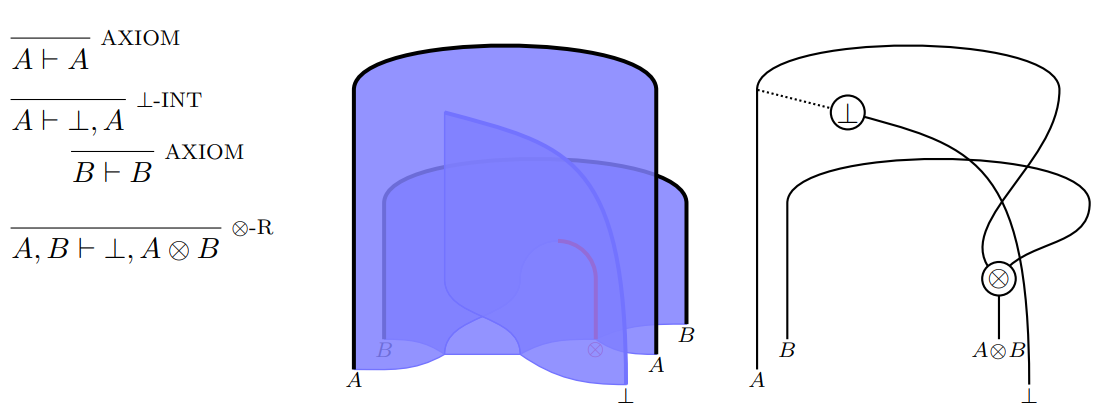
\includegraphics[width=130mm]{pictures/proof_net.png}
%\caption{3D representation of proof nets \cite[Fig. 1]{dunn} }
%\end{figure}
%
%The thinning links (drawn as dotted lines on the right hand side of this figure) can be seen to arise as a way to recover the connectivity information of the units which is lost as degeneracies in the projection from 3 to 2-dimensions.
%
%
%This is an essential difference for proof nets for monoidal categories and proof nets for linearly distributive categories. In particular, monoidal categories can be regarded as special cases of linearly distributive categories where both monoidal structures coincide and the linear distributors are the associators.  In this case, the distributor is redundant, and the 3rd dimension adds no new information. Therefore,  the calculus of thinning links which keeps track of the connectivity information of the units is not needed.  Thus, in the monoidal setting one recovers proof nets we reviewed in the previous subsection.
%
%
%
%On a separate note, linearly distributive categories have also been used to explore quantum causality \cite{sander} as well as to give toy models for infinite dimensional quantum processes  \cite{muc}.  Therefore, there is also motivation for understanding proof nets in the non-monoidal setting in the context of exploring quantum mechanics from a categorical perspective, although it is not the focus of this thesis.




%

\subsection{(De)composing props}
\label{subsec:internal}
%\begin{definition}
%\label{def:monad}
%%monad
%\end{definition}
%
%
%
%\begin{definition}
%\label{def:span}
%
%%bicategory of spans, cospans
%\end{definition}
%
%
%\begin{definition}
%\label{def:rel}
%
%%bicategory of relations, corelations
%\end{definition}



In this section we review some aspects of internal category theory so that we can compose props via distributive law.

% basic results regarding internal categories.  Unless explicitly referenced, the results and definitions of internal category theory contained within this chapter can be found within a standard textbook in category theory (eg. \cite{maclane}). 





One way to combine monoidal theories is via pushout.  We generalize the analagous result of \cite[Proposition 2.51]{ih} to the multicoloured setting:

THIS DEFINITION IS WRONG... FIX IT TODO
\begin{lemma}
Take three (symmetric) monoidal theories

$$T_0=({\sf Ob}_0,\Sigma_0 ,E_0 ), \ T_1=({\sf Ob}_1,\Sigma_1 ,E_1 ), \ T_2=({\sf Ob}_2,\Sigma_2 ,E_2 )$$

such that $\bar{T_0}$ is a sub-pro(p) of both $\bar{T_1}$ and $\bar{T_2}$ and $\Sigma_0 \subseteq \Sigma_1,\Sigma_2$.
Then the pushout of the diagram $\bar{T_1} \leftarrow \bar{T_0} \rightarrow \bar{T_2}$  in the category of strict (symmetric) monoidal categories is presented by the (symmetric) monoidal theory:

$$
( {\sf Ob}_1 +_{{\sf Ob}_0} {\sf Ob}_2, \Sigma_0+\Sigma_1, E_1 \cup E_2 \cup E_3 )
$$

\end{lemma}

In practice, we usually won't be so explicit about the pushout of (symmetric) monoidal theories.  Rather, we will present a set of generators and multiple equations between different subsets of generators.  Indeed, we have done this many times up to this point when glueing (symmetric) monoidal theories together.  



However, there is a more refined notion of composition of pro(p)s; to expose which, we first need to review  a considerable amount of internal category theory.


\subsubsection{Internal categories and strict factorization systems}




\begin{definition}
\label{def:monad}
Given a bicategory $\mathcal B$, there is a bicategory of monads in $\mathcal B$, $\Mnd({\mathcal B})$ with:

\begin{description}
\item[0-cells:]

{\bf Monads} are tuples $(X,T,\mu,\eta)$ in $\mathcal B$.  Where $X$ is a $0$-cell $T:X\to X$ is a $1$-cell and  $\mu:T^2 \to T$ and $\eta:1_X\to T$ are $2$-cells satisfying the associativity and unit laws:


\hfil$
\xymatrix{
T^3 \ar[r]^{T;\mu} \ar[d]_{\mu; T}
  & T^2 \ar[d]^\mu\\
T^2\ar[r]_{\mu} & T
}
\hspace*{1cm}
\xymatrix{
T \ar[r]^{\eta; T} \ar[d]_{ T;\eta} \ar@{=}[dr] & T^2 \ar[d]^\mu\\
T^2 \ar[r]_{\mu} & T
}
$


\item[1-cells:] {\bf Monad maps}   $(F,\lambda):(X,T,\mu^T, \eta^T)\to (Y,S,\mu^S, \eta^S)$.  Where  $F:X\to Y$ is a $1$-cell and $\lambda:F;S\to T;F$ is a 2-cell preserving the unit and multiplication as follows:

\hfil$
\xymatrix{
F \ar[r]^{\eta^S;F} \ar[dr]_{F;\eta^T} 
  & S;F \ar[d]^{\lambda}\\
  &  F;T
}
\hspace*{1cm}
\xymatrix{
S^2; F \ar[r]^{S;\lambda} \ar[d]_{\mu^S;F}
 & S;F;T \ar[r] ^{\lambda; T}
 & F;T^2 \ar[d]^{F;\mu^T}\\
S;F \ar[rr]_{\lambda}
 &
 & F;T
}
$
\item[2-cells:] {\bf Intertwiners} between monad maps $(F,\lambda) \to (G;\chi)$ are 2-cells $\phi: F\to G$ such that:

$$
\xymatrix{
S;F \ar[r]^{S;\phi} \ar[d]_{\lambda}
 & S;G \ar[d]^{\chi}\\
F;T \ar[r]_{\phi;T}
 & G;T
}
$$
\end{description}
\end{definition}

This allows us to define the following:

\begin{definition}
\label{def:internalcat}

%Internal category
Given a category $\mathcal V$ with finite pullbacks $\mathcal V$, a $\mathcal V$-{\bf internal category} is a monad in $\Span(\mathcal V)$.
\end{definition}


\begin{example}
\label{ex:internalcat}
Monads internal to $\Span(\Set)$ are in bijection with small categories.
\end{example}

Let us upack this a bit.  A small category has a {\em set} $\sf Ob$ of objects, and a {\em set} {\sf Ar} of maps.  There is a map ${\sf dom}:{\sf Ar}\to {\sf Ob}$ which picks out the domain of maps and another map  ${\sf codom}:{\sf Ar}\to {\sf Ob}$ picking out the codomain.  That is to say, a span of sets:
$$
S=\xymatrix{
& {\sf Ar} \ar[dl]_{{\sf dom}} \ar[dr]^{\sf codom}\\
{\sf Ob} & & {\sf Ob}
}
$$

Composition of maps is a function which takes maps $f:X\to Y$ and $g:Y\to X$ to a new map $(f;g):X\to Y$.   This is asking for a 2-cell $\mu:S^2\to S$ in $\Span(\Set)$; the pullback picks out the composable maps and composes them.  The associativity of composition corresponds to the associativity of $\mu$ as a semigroup.
On the other hand, the unit of a small category is a function from ${\sf Ob}$ to $S$, picking out for every object $X$, a map $1_X$ with domain and codomain $X$ , that is to say, a 2-cell $\mu:1_{\sf Ob}\to S$.  The unitality of composition is the unitality of the monad.

One should be careful to notice that the $1$-cells in $\Mnd(\Span(\Set))$ do not correspond to functors between small categories.  This structure naturally arizes by considering the analagous {\em double category} (although, this is out of scope for this thesis).


There is a canonical way to compose monads, and thus small categories:

\begin{definition}
Given two monads $\mathbb{L}=(X,L,\mu^L, \eta^L)$ and $\mathbb{R}=(X,R,\mu^R, \eta^R)$ in a bicategory $\cal B$, a distributive law of $R$ over $L$ is a 2-cell $\lambda:R;L\to L;R$ in $\mathcal B$ satisfying the following coherence equations:


\hfil
$
\xymatrix{
R \ar[dr]^{R;\eta^L} \ar[d]_{\eta^L;R}\\
 L;R \ar[r]_{\lambda}
 & R;L
}
\hspace*{1cm}
\xymatrix{
L^2;R \ar[r]^{L;\lambda} \ar[d]_{\mu^L;R}
 & L;R;L \ar[r]^{\lambda;L}
  & R;L;L \ar[d]^{R;\mu^L}\\
L;R \ar[rr]_{\lambda}
  & 
  &R;L
}
$

\hfil
$
\xymatrix{
R \ar[dr]^{\eta^R;L} \ar[d]_{L;\eta^R}\\
 L;R \ar[r]_{\lambda}
 & R;L
}
\hspace*{1cm}
\xymatrix{
L;R^2 \ar[r]^{\lambda;R} \ar[d]_{L;\mu^R}
 & R;L;R \ar[r]^{R;\lambda}
  & R;R;L \ar[d]^{\mu^R;L}\\
L;R \ar[rr]_{\lambda}
  & 
  &R;L
}
$
\end{definition}


Distributive laws of monads are compositions in the following sense:

\begin{lemma}
Given a distributive law of monads $\lambda:R;L\to L;R$, the 1-cell
$L;R$ has a monad structure with:

\begin{tabular}{lc}
{\bf unit:} & $\eta^{L;R}:=1_{X} \xrightarrow{\eta^L;\eta^R} L;R $\\
{\bf multiplication:} & $\mu^{L;R}:=(L;R)^2 \xrightarrow{1_X; \lambda ; 1_X} L;L;R;R \xrightarrow{\mu^L;\mu^R} L;R$
\end{tabular}

\end{lemma}


There is a very concise way of viewing distributive laws:

\begin{lemma}[{\cite[\S 6]{street}}]
Distributive laws of monads in a bicategory $\cal B$ are precisely monads in $\Mnd({\cal B})$.
\end{lemma}


The following notion allows one to factorize the maps in categories:


\begin{definition}[{\cite[\S 6.2]{grandis}}]
A {\bf strict factorization system} on a category $\X$ is a pair of subcategories $(\mathbb{L},\mathbb{R})$ of $\X$ with the same objects as $\X$, such that every map in $\X$ can be uniquely factored into a map in $\mathbb{L}$ followed by a map in  $\mathbb{R}$.


That is to say every map $f:X\to Y$ factorizes as follows


$$
\xymatrix{
X  \ar[rr]^{f} \ar[dr]_{\ell \in {\mathbb L}} &       & Y\\
   & A \ar[ur]_{r \in {\mathbb R}}
}
$$

such that given another such factorization
$$
\xymatrix{
X  \ar[rr]^{f} \ar[dr]_{\ell' \in {\mathbb L}} &       & Y\\
   & A' \ar[ur]_{r' \in {\mathbb R}}
}
$$

then the following diagram commutes:

$$
\xymatrixrowsep{10mm}
\xymatrixcolsep{50mm}
\xymatrix{
X \ar@{=}[d] \ar[r]^{\ell}   & A  \ar@{=}[d] \ar[r]^{r} & Y \ar@{=}[d]\\
X   \ar[r]_{\ell'}                & A' \ar[r]_{r'} & Y
}
$$
\end{definition}

\begin{lemma}[{\cite[Theorem 3.8]{rosebrugh}}]
\label{lemma:rosebrugh}
Strict factorization systems of small categories $(\mathbb L,\mathbb R)$ are precisely distributive laws of $\mathbb R$ over $\mathbb L$ , viewed as monads in $\Span(\Set)$.
\end{lemma}

Therefore, a distributive law of small categories can be regarded as a way to uniquely factorize maps into two disjoint subcategories $\mathbb{L};\mathbb{R}$; so that if a composite is out of order, there is a rule $\mathbb{L};\mathbb{R}\to \mathbb{R};\mathbb{L}$ to push them past each other uniquely.


By changing $\Set$ to the category of monoids, \cite{lack} observed that one can recover the appropriate notion of a strict factorization system of pros.  First recall the category of monoids: 

\begin{definition}
\label{def:monoid}
Let $\Mon$ denote the category with set-monoids as objects and monoid homorphisms as morphisms.
\end{definition}

$\Mon$ has finite pullbacks, so one can define categories within it.  We already have introduced these categories in other terms:


\begin{lemma}[{\cite[\S 2.3]{lack}}]
\label{def:internalmonoidalcat}

Monads in $\Span(\Mon)$ are in bijection with small strict monoidal categories.
\end{lemma}

%Indeed, in analogy to the case for small catgories, a distributive law $\X;\Y$ of two small strict monoidal categories is precisely a way to combine the two theories, respecting their monoidal structure,  where the maps can be uniquely factored into maps in $\X$ followed by maps in $\Y$.

There is an obvious analogue of strict factorizations for small strict monoidal categories, which I shall call monoidal strict factorization systems.  In this setting $\mathbb L$ and $\mathbb R$ are small strict monoidal subcategories of $\X$

Therefore, reproducing Lemma \ref{lemma:rosebrugh} internal to $\Mon$ we have:

\begin{lemma}[{\cite[Theorem 3.8]{lack}}]
Monoidal strict factorization systems of small categories $(\mathbb L,\mathbb R)$ are precisely distributive laws of $\mathbb R$ over $\mathbb L$ , viewed as monads in $\Span(\Mon)$.
\end{lemma}

Distributive laws of monoidal theories yield a monoidal theory for the composite internal monoidal category. The two theories are combined,  plus rules to push the generators past each other.  This follows immediately from the analysis of distributive laws of props of \cite[Theorem 3.8]{lack}, where a prop is a strict monoidal category on the free monoid $\N$.  

\begin{lemma}
Take two monoidal theories

$$
R=({\sf Ob},\Sigma_R ,E_R ), \ L=({\sf Ob},\Sigma_L ,E_L )
$$

With the same objects.  Regard their corresponding pros $\bar{R}$ and $\bar{L}$ as monads in $\Span(\Mon)$ such that there is a distributive $\lambda:\bar{R};\bar{L} \Rightarrow \bar{L};\bar{R}$.  Where $ \bar{L};\bar{R}$ is a strict monoidal category and both $\bar L$ and $\bar R$ are strict monoidal subcategories of   $\bar{L};\bar{R}$


Then the monoidal theory for the composite pro $\bar{L};\bar{R}$ is given by 
$$
({\sf Ob}, \Sigma_R\cup \Sigma_L, E_R\cup E_L \cup E_\lambda)
$$

where $\lambda$ is the set of equations dictating the unique ways in which the maps in $R$ can be pushed past those in $L$.
\end{lemma}


Now we can see, for example, how the pro $\sfa$ arizes in this manner:

\begin{definition}
Consider the distributive law of pros of a comonoid $\zcirc$ over a monoid $\zcirc$:
\begin{align*}
\m; \m^\op;&
    \begin{tikzpicture}[rotate=90]
	\begin{pgfonlayer}{nodelayer}
		\node [style=Z] (0) at (-6.25, 0.25) {};
		\node [style=none] (1) at (-7, 0.25) {};
		\node [style=none] (2) at (-4.75, 0.25) {};
		\node [style=Z] (3) at (-5.5, 0.25) {};
	\end{pgfonlayer}
	\begin{pgfonlayer}{edgelayer}
		\draw (0) to (1.center);
		\draw (3) to (2.center);
		\draw [bend right, looseness=1.25] (3) to (0);
		\draw [bend right, looseness=1.25] (0) to (3);
	\end{pgfonlayer}
  \end{tikzpicture}
  \eref{special}
  \begin{tikzpicture}[rotate=90]
	\begin{pgfonlayer}{nodelayer}
		\node [style=none] (0) at (-7, 0.25) {};
		\node [style=none] (1) at (-6, 0.25) {};
	\end{pgfonlayer}
	\begin{pgfonlayer}{edgelayer}
		\draw (1.center) to (0.center);
	\end{pgfonlayer}
  \end{tikzpicture},
  \hspace*{.5cm}
  \begin{tikzpicture}[rotate=90]
	\begin{pgfonlayer}{nodelayer}
		\node [style=Z] (0) at (-7, -0) {};
		\node [style=Z] (1) at (-6.25, 0.5) {};
		\node [style=none] (2) at (-7, 0.75) {};
		\node [style=none] (3) at (-7.75, 0.75) {};
		\node [style=none] (4) at (-7.75, -0) {};
		\node [style=none] (5) at (-6.25, -0.25) {};
		\node [style=none] (6) at (-5.5, -0.25) {};
		\node [style=none] (7) at (-5.5, 0.5) {};
	\end{pgfonlayer}
	\begin{pgfonlayer}{edgelayer}
		\draw (6.center) to (5.center);
		\draw [in=-30, out=180, looseness=1.00] (5.center) to (0);
		\draw (1) to (0);
		\draw [in=0, out=150, looseness=1.00] (1) to (2.center);
		\draw (2.center) to (3.center);
		\draw (0) to (4.center);
		\draw (1) to (7.center);
	\end{pgfonlayer}
  \end{tikzpicture}
  \eref{frobl}
  \begin{tikzpicture}[rotate=90]
	\begin{pgfonlayer}{nodelayer}
		\node [style=none] (0) at (-4.75, -0.25) {};
		\node [style=Z] (1) at (-5.5, -0) {};
		\node [style=none] (2) at (-7, -0.25) {};
		\node [style=Z] (3) at (-6.25, 0) {};
		\node [style=none] (4) at (-4.75, 0.25) {};
		\node [style=none] (5) at (-7, 0.25) {};
	\end{pgfonlayer}
	\begin{pgfonlayer}{edgelayer}
		\draw [in=-30, out=180, looseness=1.25] (0.center) to (1);
		\draw (3) to (1);
		\draw [in=180, out=30, looseness=1.25] (1) to (4.center);
		\draw [in=0, out=-150, looseness=1.25] (3) to (2.center);
		\draw [in=0, out=150, looseness=1.25] (3) to (5.center);
	\end{pgfonlayer}
\end{tikzpicture}
,\hspace*{.5cm}
  \begin{tikzpicture}[rotate=90,xscale=-1]
	\begin{pgfonlayer}{nodelayer}
		\node [style=Z] (0) at (-7, -0) {};
		\node [style=Z] (1) at (-6.25, 0.5) {};
		\node [style=none] (2) at (-7, 0.75) {};
		\node [style=none] (3) at (-7.75, 0.75) {};
		\node [style=none] (4) at (-7.75, -0) {};
		\node [style=none] (5) at (-6.25, -0.25) {};
		\node [style=none] (6) at (-5.5, -0.25) {};
		\node [style=none] (7) at (-5.5, 0.5) {};
	\end{pgfonlayer}
	\begin{pgfonlayer}{edgelayer}
		\draw (6.center) to (5.center);
		\draw [in=-30, out=180, looseness=1.00] (5.center) to (0);
		\draw (1) to (0);
		\draw [in=0, out=150, looseness=1.00] (1) to (2.center);
		\draw (2.center) to (3.center);
		\draw (0) to (4.center);
		\draw (1) to (7.center);
	\end{pgfonlayer}
  \end{tikzpicture}
  \eref{frobr}
\begin{tikzpicture}[rotate=90]
	\begin{pgfonlayer}{nodelayer}
		\node [style=none] (0) at (-4.75, -0.25) {};
		\node [style=Z] (1) at (-5.5, -0) {};
		\node [style=none] (2) at (-7, -0.25) {};
		\node [style=Z] (3) at (-6.25, 0) {};
		\node [style=none] (4) at (-4.75, 0.25) {};
		\node [style=none] (5) at (-7, 0.25) {};
	\end{pgfonlayer}
	\begin{pgfonlayer}{edgelayer}
		\draw [in=-30, out=180, looseness=1.25] (0.center) to (1);
		\draw (3) to (1);
		\draw [in=180, out=30, looseness=1.25] (1) to (4.center);
		\draw [in=0, out=-150, looseness=1.25] (3) to (2.center);
		\draw [in=0, out=150, looseness=1.25] (3) to (5.center);
	\end{pgfonlayer}
\end{tikzpicture}
  \end{align*}

Which we recall is the  pro {\sf sfa} for the free  special  Frobenius algebra.

\end{definition}




%
%
%
%\begin{lemma}[{\cite[?]{lack}}]
%{\sfa} is a presentation for $(\Span^\sim(\FinOrdMonot^\op),+)$.
%\end{lemma}
%\begin{proof}
%The idea is that a given a two cospans, the pushout of the cospan in the middle induces a mapping taking cospans to spans in $\FinOrdMonot$, but we know that the skeleton of $\FinMonot$ is $\m$.  Therefore, it remains to check all of the critical pairs which occur in $\m^\op;\m$.  The special Frobenius laws are precisely the way to resolve these critical pairs and push the generators in $\m^\op$ past $\m$.
%\end{proof}
%


The unique normal form induced by this distributive will be widely used throughout this thesis:



\begin{lemma}[Non-commutative special spider normal form]
The circuits in $\sf sfa$ generated by the connected components of the Frobenius algebra have a unique normal form. We use the ``spider notation'' on the right to refer to these simply connected components:


$$
\begin{tikzpicture}
	\begin{pgfonlayer}{nodelayer}
		\node [style=none] (0) at (1.5, 1.75) {};
		\node [style=none] (1) at (2.75, 1.75) {};
		\node [style=none] (2) at (2, 1.75) {};
		\node [style=none] (3) at (2.45, 1.75) {$\cdots$};
		\node [style=none] (4) at (2.75, 3.25) {};
		\node [style=none] (5) at (2, 3.25) {};
		\node [style=none] (6) at (1.5, 3.25) {};
		\node [style=none] (7) at (2.45, 3.25) {$\cdots$};
		\node [style=Z] (8) at (2, 2.5) {};
	\end{pgfonlayer}
	\begin{pgfonlayer}{edgelayer}
		\draw [in=-90, out=45] (8) to (4.center);
		\draw (8) to (5.center);
		\draw [in=135, out=-90] (6.center) to (8);
		\draw [in=90, out=-150] (8) to (0.center);
		\draw (2.center) to (8);
		\draw [in=90, out=-30] (8) to (1.center);
	\end{pgfonlayer}
\end{tikzpicture}
:=
\begin{tikzpicture}
	\begin{pgfonlayer}{nodelayer}
		\node [style=Z] (0) at (1.25, 3) {};
		\node [style=Z] (1) at (0.5, 4) {};
		\node [style=Z] (2) at (1.25, 2.25) {};
		\node [style=Z] (3) at (0.5, 1.25) {};
		\node [style=none] (4) at (1.5, 4) {};
		\node [style=none] (5) at (1.5, 1.25) {};
		\node [style=none] (6) at (0.25, 0.5) {};
		\node [style=none] (7) at (1.5, 4.75) {};
		\node [style=none] (8) at (1.5, 0.5) {};
		\node [style=none] (9) at (0.75, 4.75) {};
		\node [style=none] (10) at (0.25, 4.75) {};
		\node [style=none] (11) at (0.75, 0.5) {};
		\node [style=none] (12) at (1, 3.25) {};
		\node [style=none] (13) at (0.5, 3.75) {};
		\node [style=none] (14) at (0.5, 1.5) {};
		\node [style=none] (15) at (1, 2) {};
		\node [style=none] (16) at (0.75, 3.5) {$\ddots$};
		\node [style=none] (17) at (0.75, 1.75) {$\reflectbox{$\ddots$}$};
		\node [style=none] (18) at (1.2, 0.5) {$\cdots$};
		\node [style=none] (19) at (1.2, 4.75) {$\cdots$};
	\end{pgfonlayer}
	\begin{pgfonlayer}{edgelayer}
		\draw (7.center) to (4.center);
		\draw [in=105, out=-90] (10.center) to (1);
		\draw [in=60, out=-90, looseness=0.75] (4.center) to (0);
		\draw [in=-90, out=75] (1) to (9.center);
		\draw [in=300, out=90] (5.center) to (2);
		\draw [in=90, out=-120] (3) to (6.center);
		\draw [in=90, out=-60] (3) to (11.center);
		\draw (8.center) to (5.center);
		\draw (0) to (2);
		\draw (3) to (14.center);
		\draw (15.center) to (2);
		\draw (13.center) to (1);
		\draw (0) to (12.center);
	\end{pgfonlayer}
\end{tikzpicture}
$$

Because the connected circuits are reducible to each other, spiders connected by wires fuse:


$$
\begin{tikzpicture}
	\begin{pgfonlayer}{nodelayer}
		\node [style=none] (32) at (20.25, -0.5) {};
		\node [style=none] (33) at (19.25, -0.5) {};
		\node [style=none] (34) at (19.75, -0.5) {$\cdots$};
		\node [style=none] (35) at (19.25, -2.75) {};
		\node [style=Z] (36) at (19.75, -1.25) {};
		\node [style=none] (37) at (20.75, -0.5) {};
		\node [style=none] (38) at (20.25, -2.75) {$\cdots$};
		\node [style=none] (39) at (19.75, -2.75) {};
		\node [style=Z] (40) at (20.25, -2) {};
		\node [style=none] (41) at (20.75, -2.75) {};
		\node [style=none] (42) at (20, -1.5) {\reflectbox{$\ddots$}};
	\end{pgfonlayer}
	\begin{pgfonlayer}{edgelayer}
		\draw [in=-135, out=90] (35.center) to (36);
		\draw [in=-90, out=56] (36) to (32.center);
		\draw [in=124, out=-90] (33.center) to (36);
		\draw [in=-124, out=90] (39.center) to (40);
		\draw [in=90, out=-56] (40) to (41.center);
		\draw [in=-90, out=45] (40) to (37.center);
		\draw [bend right=45, looseness=1.25] (40) to (36);
		\draw [bend right=45, looseness=1.25] (36) to (40);
	\end{pgfonlayer}
\end{tikzpicture}
=
\begin{tikzpicture}
	\begin{pgfonlayer}{nodelayer}
		\node [style=none] (11) at (4, -0.5) {};
		\node [style=none] (12) at (3, -0.5) {};
		\node [style=none] (13) at (3.5, -0.5) {$\cdots$};
		\node [style=none] (14) at (2.5, -2) {};
		\node [style=none] (15) at (3.5, -1.25) {};
		\node [style=none] (16) at (4.5, -0.5) {};
		\node [style=none] (17) at (3.5, -2) {$\cdots$};
		\node [style=none] (18) at (3, -2) {};
		\node [style=Z] (19) at (3.5, -1.25) {};
		\node [style=none] (20) at (4, -2) {};
	\end{pgfonlayer}
	\begin{pgfonlayer}{edgelayer}
		\draw [in=-150, out=90] (14.center) to (15);
		\draw [in=-90, out=56] (15) to (11.center);
		\draw [in=124, out=-90] (12.center) to (15);
		\draw [in=-124, out=90] (18.center) to (19);
		\draw [in=90, out=-56] (19) to (20.center);
		\draw [in=-90, out=30] (19) to (16.center);
	\end{pgfonlayer}
\end{tikzpicture}
$$
\end{lemma}

We will also use the following related result:

\begin{lemma}[Non-commutative spider normal form]

In the case of the prop $\sf fa$ when the Frobenius algebra is not special, then the spider theorem only holds for simply connected circuits.  For example, given a Frobenius algebra $\xcirc$:


$$
\begin{tikzpicture}
	\begin{pgfonlayer}{nodelayer}
		\node [style=none] (0) at (1.5, -0.5) {};
		\node [style=none] (1) at (0.5, -0.5) {};
		\node [style=none] (2) at (1, -0.5) {$\cdots$};
		\node [style=none] (3) at (0.5, -2.75) {};
		\node [style=X] (4) at (1, -1.25) {};
		\node [style=none] (5) at (2, -0.5) {};
		\node [style=none] (6) at (1.5, -2.75) {$\cdots$};
		\node [style=none] (7) at (1, -2.75) {};
		\node [style=X] (8) at (1.5, -2) {};
		\node [style=none] (9) at (2, -2.75) {};
	\end{pgfonlayer}
	\begin{pgfonlayer}{edgelayer}
		\draw [in=-124, out=90] (3.center) to (4);
		\draw [in=-90, out=56] (4) to (0.center);
		\draw [in=124, out=-90] (1.center) to (4);
		\draw [in=-124, out=90] (7.center) to (8);
		\draw [in=90, out=-56] (8) to (9.center);
		\draw [in=-90, out=56] (8) to (5.center);
		\draw (8) to (4);
	\end{pgfonlayer}
\end{tikzpicture}
=
\begin{tikzpicture}
	\begin{pgfonlayer}{nodelayer}
		\node [style=none] (11) at (4, -0.5) {};
		\node [style=none] (12) at (3, -0.5) {};
		\node [style=none] (13) at (3.5, -0.5) {$\cdots$};
		\node [style=none] (14) at (2.5, -2) {};
		\node [style=none] (15) at (3.5, -1.25) {};
		\node [style=none] (16) at (4.5, -0.5) {};
		\node [style=none] (17) at (3.5, -2) {};
		\node [style=none] (18) at (3, -2) {};
		\node [style=X] (19) at (3.5, -1.25) {};
		\node [style=none] (20) at (4, -2) {};
	\end{pgfonlayer}
	\begin{pgfonlayer}{edgelayer}
		\draw [in=-150, out=90] (14.center) to (15);
		\draw [in=-90, out=56] (15) to (11.center);
		\draw [in=124, out=-90] (12.center) to (15);
		\draw [in=-124, out=90] (18.center) to (19);
		\draw [in=90, out=-56] (19) to (20.center);
		\draw [in=-90, out=30] (19) to (16.center);
	\end{pgfonlayer}
\end{tikzpicture}
$$

This does not arise from a distributive law of props.  This should arize instead from a distributive law of polycategories, however, we won't go into any more detail here.  We will however discuss polycategories in Chapter \ref{chap:grothendieck} which will make this clearler.
\end{lemma}




\subsubsection{Internal profunctors and factorization systems over subcategories}

We want to be able to take distributive laws of two categories which both share some structure.  For example, what is the appropriate notion of distributive law of small strict symmetric monoidal categories where the braiding of both categories are identified with each other?  For this, we can regard the structure of a subcategory as an action on the larger category; formally, this is a certain kind of bimodule:



\begin{definition}
Given a bicategory $\mathcal B$ with coequalizers,
the bicategory of bimodules in $\mathcal B$, $\Mod(\mathcal{B})$ has:

\begin{description}
\item[\ \ 0-cells:] Monads in $\mathcal B$.
\item[\ \ 1-cells:] A $1$-cell between monads $\mathbb{T}=(X,T,\mu^T,\eta^T)\to \mathbb{S}=(Y,S,\mu^S,\eta^S)$ is a $(\mathbb{T},\mathbb{S})$-{\bf bimodule}.  That is a triple $(F,\tau,\rho)$ where  $F:X\to Y$ is a 1-cell in $\mathcal B$ and $\tau:S;F\to F$ and $\rho:F;T\to F$ are  2-cells (the left and right {\bf actions}, respectively) satisfying the following coherence equations: 

\begin{description}

\item[$(F,\tau,\rho)$ is a left $\mathbb{S}$-module:]
$$
\xymatrix{
 S;S;F \ar[r]^{\ \mu^S;F} \ar[d]_{S;\tau}
  & S;F \ar[d]^{\tau}
\\S;F \ar[r]_{\tau}
  &F
}\ ,
\hspace{.5cm}
\xymatrix{
  F \ar@{=}[dr] \ar[d]_{\eta^S;F} 
\\S;F \ar[r]_{\tau}
   & F
}
$$

\item[$(F,\tau,\rho)$ is a right $\mathbb{S}$-module:]
$$
\xymatrix{
 F;T;T \ar[r]^{\ F;\mu^T} \ar[d]_{\rho;T}
  & F;T \ar[d]^{\rho}
\\F;T \ar[r]_{\rho}
  &F
}\ ,
\hspace{.5cm}
\xymatrix{
  F \ar@{=}[dr] \ar[d]_{F;\eta^T} 
\\F;T \ar[r]_{\rho}
   & F
}
$$

\item[Module compatibility:]
$$
\xymatrix{
S;F;T \ar[r]^{S;\rho} \ar[d]_{\tau;T}
& S;F \ar[d]^{\tau}\\
F;T \ar[r]_{\rho}
& F
}
$$

\end{description}

Given a $(\mathbb{S},\mathbb{T})$-bimodule $(F,\tau,\rho)$ and a  $(\mathbb{T},\mathbb{U})$-bimodule $(G,\tau,\rho')$, the composite has 1-cell given by the coequalizer:

$$
\xymatrix{
F;T;G  \ar@<-.5ex>[r]_{T;\rho'} \ar@<.5ex>[r]^{\tau;T} & F;G \ar[r] &F \otimes_T G 
}
$$

with left and right actions induced by $\tau$ and $\rho'$.

The identity 1-cell on a monad is the monad itself considered as a bimodule over itself.

\item[\ \ 2-cells:] A 2-cell between $(\mathbb{S},\mathbb{T})$-bimodules $(F,\rho,\tau)\to (G,\rho',\tau')$ is a 2-cell $\phi:F\to G$ in $\mathcal{B}$ satisfying the following coherence conditions:

$$
\xymatrix{
  S;F \ar[r]^{\tau}  \ar[d]_{S;\phi}
   & F \ar[d]^{\phi}
\\S;G \ar[r]_{\tau'}
   &G
}
\hspace*{.5cm}
\xymatrix{
  F;T \ar[r]^{\rho}  \ar[d]_{\phi;T}
   & F \ar[d]^{\phi}
\\G;T \ar[r]_{\rho'}
   &G
}
$$

Composition and identities are given pointwise in $\mathcal B$.
\end{description}
\end{definition}

Now we can look at modules of internal categories:

\begin{definition}
\label{def:internalprof}
Given a category $\mathcal V$ with finite pullbacks and coequalizers preserving them, let $\mathcal V$-$\Prof:=\Mod(\Span(\mathcal V))^\op$ denote the bicategory of $\mathcal V$-{\bf internal profunctors}.  
The 1-cells of $\mathcal V$-$\Prof$ are called (internal) {\bf  profunctors}.
The tensor product of bimodules of internal categories is the (internal) {\bf coend}.
\end{definition}

This is a special case of ordinary profunctors, attributed to B\'enabou \cite{???}:

\begin{example}
$\Set$-$\Prof$ is the category of profunctors between small categories.
\end{example}


We related distributive laws in internal categories to factorization systems.  To do so we introduce the following notation:

\begin{definition}
Let $\Iso(\X)$ denote the groupoid  of all isomorphisms of $\X$.
\end{definition}

There is a notion of factorization system where the factorization need only hold up to isomorphism:
\begin{definition}
An {\bf orthogonal factorization system} on a category $\X$ is a pair of subcategories $(\mathbb{L},\mathbb{R})$ of $\X$ with the same objects as $\X$, where $\mathbb{L}$ and $\mathbb{R}$ contain all isomorphisms in $\X$, and moreover, where every map in $\X$ factors as a map in  $\mathbb{L}$, followed by one $\mathbb{R}$ up to unique isomorphism.


That is to say every map $f:X\to Y$ factorizes as follows


$$
\xymatrix{
X  \ar[rr]^{f} \ar[dr]_{\ell \in {\mathbb L}} &       & Y\\
   & A \ar[ur]_{r \in {\mathbb R}}
}
$$

such that given another such factorization
$$
\xymatrix{
X  \ar[rr]^{f} \ar[dr]_{\ell' \in {\mathbb L}} &       & Y\\
   & A' \ar[ur]_{r' \in {\mathbb R}}
}
$$

then there is a unique isomorphism $\phi:A\to A'$ such that the following diagram commutes:

$$
\xymatrixrowsep{10mm}
\xymatrixcolsep{50mm}
\xymatrix{
X \ar@{=}[d] \ar[r]^{\ell}   & A  \ar@{-->}[d]^{\phi} \ar[r]^{r} & Y \ar@{=}[d]\\
X   \ar[r]_{\ell'}                & A' \ar[r]_{r'} & Y
}
$$

\end{definition}

This is the same as a distributive law of monads in $\Set$-$\Prof$ over $\Iso(\X)$:

\begin{lemma}[{\cite[Theorem 5.9]{rosebrugh}}]
An orthogonal factorization system $(\mathbb{L},\mathbb{R})$ on a small category $\X$ is precisely a distributive law of monads between $\mathbb{L}$ and $\mathbb{R}$, regarded as $\Iso(\X)$-bimodules.
\end{lemma}

We have already discussed two examples of orthogonal factorization systems in order to define categories of internal relations:

\begin{example}
Given a finitely complete category $\X$, the category $\Span^\sim(\X)$ has an orthogonal factorization system where:

$$\mathbb{L}:=\{ \xymatrix{X & X \ar@{=}[l] \ar[r]^{f } & Y}    \  | \ \forall f \in \X(X,Y) \}\, \hspace*{.2cm}
\mathbb{R}:=\{\xymatrix{Y & X \ar@{=}[r] \ar[l]_{f } & X}    \  | \ \forall f \in \X(X,Y)  \}$$

\end{example}


\begin{example}
Regular categories have orthogonal factorization systems given by $\mathbb{L}$ the regular epimorphisms, and $\mathbb R$ the monomorphisms.
\end{example}



By asking that $\X$ is a small strict monoidal category and  $\mathbb{L}$ and $\mathbb{R}$ are strict monoidal subcategories of $\X$, the notion of an orthogonal factorization system is adapted immediately to monoidal categories. And there is an alagous correspondence  between $\mathbb{L}$ and $\mathbb{R}$, regarded as $\Iso(\X)$-bimodules in $\Span(\Mon)$.  However, this is not satisfying for our purposes.

 In the most basic setting, the shared structure of small strict {\em symmetric} monoidal categories on the same set of objects is the permutations on the objects .  Indeed, this is the basis Lack's work on composing props \cite{lack}. Factorizations up permutations are clearly not strict; and they are only an orthogonal factorization system when all isomorphisms are permutation.  For our purposes, we wil also need to consider cases when $\mathbb J$ is not even a groupoid!  We will recall a considerably more general notion to this end:

\begin{definition}[{\cite[Definition 4.10]{lawvere}}]
Let $\X$ be a category equipped with a subcategory $\mathbb J$ with the same objects.

A {\bf factorization system of $\X$ over $\mathbb J$} consists of a pair of subcategories $(\mathbb L,\mathbb R)$ of $\X$ with the same objects as $\X$ such that $\mathbb J$ is a subcategory of both $\mathbb L$ and $\mathbb R$.  And moreover, every map in $\X$ factorizes into maps in $\mathbb L$ followed by maps in $\mathbb R$ uniquely up to zig-zags in $\mathbb J$.

That is to say, given any map $f:X\to Y$ in $\X$, there is a factorization

$$
\xymatrix{
X  \ar[rr]^{f} \ar[dr]_{\ell \in {\mathbb L}} &       & Y\\
   & A \ar[ur]_{r \in {\mathbb R}}
}
$$

such that given another such factorization

$$
\xymatrix{
X  \ar[rr]^{f} \ar[dr]_{\ell' \in {\mathbb L}} &       & Y\\
   & A' \ar[ur]_{r'  \in {\mathbb R}}
}
$$

there exists a smallest natural number $n$, such that  for $j \in [0,n)$, there are $n$ factorizations:


$$
\xymatrix{
X  \ar[rr]^{f} \ar[dr]_{\ell_j\in {\mathbb L}} &       & Y\\
   & A_j \ar[ur]_{r_j \in {\mathbb R}}
}
$$

such that there exists $\mathbb J$

$$
\xymatrix{
A \ar[r]^{\phi_0}
& A_0 
& A_1 \ar[l]_{\phi_1} \ar[r]^{\phi_2}
& A_2 
& A_3 \ar[l]_{\phi_3} \ar[r]^{\phi_4}
&\cdots
& A_{n-1} \ar[l]_{\phi_{n-1}} \ar[r]^{\phi_n}
& A'
}
$$

which uniquely make the following diagram commute:


$$
\xymatrixrowsep{10mm}
\xymatrixcolsep{50mm}
\xymatrix{
X   \ar[r]^{\ell}\ar@{=}[d]              & A \ar@{-->}[d]^{\phi_0} \ar[r]^{r}                                               & Y \ar@{=}[d]\\
X   \ar[r]^{\ell_0}\ar@{=}[d]          & A_0  \ar[r]^{r_0}                                                                          & Y\ar@{=}[d]\\
X   \ar[r]^{\ell_1}\ar@{=}[d]           & A_1 \ar@{-->}[u]_{\phi_1} \ar@{-->}[d]^{\phi_2} \ar[r]^{r_1}  & Y \ar@{=}[d]\\
X   \ar[r]^{\ell_2}\ar@{=}[d]           & A_2 \ar[r]^{r_2}                                                                             & Y \ar@{=}[d]\\
X   \ar[r]^{\ell_3}\ar@{=}[d]         & A_ 3\ar@{-->}[u]_{\phi_3} \ar@{-->}[d]^{\phi_4}\ar[r]^{r_3}   & Y \ar@{=}[d]\\
 \vdots\ar@{=}[d]         & \vdots & \vdots \ar@{=}[d] \\
X   \ar[r]^{\ell_{n-1}}\ar@{=}[d]   & A_{n-1}  \ar@{-->}[u]_{\phi_{n-1}} \ar@{-->}[d]^{\phi_n}  \ar[r]^{r_{n-1}}         & Y    \ar@{=}[d]\\
X   \ar[r]^{\ell'}                         & A'   \ar[r]^{r'} & Y
}
$$

\end{definition}

This specializes to strict factorization systems when $\mathbb J$ contains exactly the identities on all objects; and to orthogonal factorization systems when it contains all isomorphisms. 


Suppose that  $\mathbb J $ is not a groupoid and we tried to replace the definition of an orthogonal factorization system $(\mathbb L, \mathbb R)$ with one where the unique mediating map is merely in $\mathbb J$.


Then if want to reduce a map in the composite
$$\mathbb{L} \otimes_{\mathbb J} \otimes \mathbb{R} \otimes_{\mathbb J}  \cdots \otimes_{\mathbb J} \mathbb{L} \otimes_{\mathbb J} \mathbb R  $$
 to one in 
$$\mathbb{L} \otimes_{\mathbb J} \mathbb{R}$$
then notice how $\mathbb J$ acts on $\mathbb L$ and $\mathbb R$ both on the left and and on the right.  The one action is covariant and the other is contravariant.  So there is a priori no unique way to slide all the maps in the various copies of $\mathbb J$ around and group them all together.  This unique-zig-zag condition is asking precisely for such a thing.  This is to be contrasted with the case when $\mathbb J$ is a groupoid, a map $\phi:X\to Y$ in $\mathbb J$ induces another map $\phi^{-1}:Y\to X$; where the notion of an orthogonal factorization system need only be slightly tweaked.


 Indeed, \cite{lawvere} shows that such a notion of factorization system corresponds to distributive laws of monads in $\Set$-$\Prof$.   The result is mentioned specifically for the case of distributive laws of Lawvere theories, but there is a more general fact:


\begin{lemma}
A factorization system $(\mathbb{L},\mathbb{R})$ of a small  category $\X$ over a subcategory  $\mathbb J $ is precisely a distributive law of monads  $\mathbb{R}$ over $\mathbb{L}$, both regarded as $\mathbb{J}$-bimodules in $\Span(\Sets)$.
\end{lemma}


By asking that $\X$ is a small strict monoidal category and  $\mathbb{L}$, $\mathbb{R}$ and $\mathbb{J}$ are strict monoidal subcategories, the notion of a factorization system of $\X$ over $\mathbb J$ is adapted immediately to  monoidal categories. And there is an alagous correspondence  to distributive laws of $\mathbb{R}$ over $\mathbb{L}$, regarded as $\mathbb J$-bimodules in $\Span(\Mon)$.  


To do the same for small strict symmetric monoidal categories, one must ask moreover that $\X$ is a small strict symmetric monoidal category, $\mathbb{L}$, $\mathbb{R}$ are strict symmetric monoidal subcategories of $\X$ and $\mathbb J$ is a strict symmetric monoidal subcategory of $\mathbb L$ and $\mathbb R$:

%In order to do to something similar with small strict monoidal categories, consider the following structure:
%
%
%\begin{definition}
%Let $\P_X$ denote the free strict symmetric monoidal category with objects labelled by $X$. Where $\P$ is the prop generated by a single object.
%\end{definition}
%
%
%This structure allows us to regard multicoloured props as bimodules (the case of single sorted props was originally conisdered, but this is a slight generalization):
%
%
%\begin{lemma}[{\cite[\S 4]{lack}}]
%Every multicloloured prop generated by objects $\sf Ob$ can be identified with a monad in $\Mon$-$\Prof$ on the $0$-cell $\P_{\sf Ob}$.  
%\end{lemma}
%
%The canonical left and right actions merely absorb the braids of $\P_{\sf Ob}$ into the prop on the left and right.  Note that not all monads on $\P_{\sf Ob}$ in $\Mon$-$\Prof$ are strict monoidal categories.
%
%
%The following characterization of distributive laws of props in terms of monoidal theories will prove to be useful for us:


\begin{lemma}
Take three symmetric monoidal theories

$$
R=({\sf Ob},\Sigma_R ,E_R ), \ L=({\sf Ob},\Sigma_L ,E_L ),  \ J=({\sf Ob},\Sigma_J ,E_J )
$$

with the same objects, where $\bar{J}$ embeds as a strict symmetric monoidal category within both $\bar{L}$ and $\bar{R}$.  Regard both $\bar{L}$ and $\bar{R}$ as  $\bar{J}$-bimodules, where the left and right actions are given by lifting the maps in $\bar{J}$ along this embedding.

Suppose there is a distributive law of monads in the bicategory $\Mon$-$\Prof$:

$$
\lambda:\bar{R}\otimes_{\bar{J}} \bar{L}\Rightarrow \bar{L}\otimes_{\bar{J}} \bar{R}
$$

Where $\bar{L}$ and $\bar{R}$ are canonically strict monoidal subcategories of $\bar{L}\otimes_{\bar{J}} \bar{R}$.

Then the induced prop $\bar{L}\otimes_{\bar{J}} \bar{R}$ is presented by a monoidal theory

$$
({\sf Ob}, \Sigma_R\cup \Sigma_L, E_R\cup E_L \cup E_\lambda)
$$

where $E_\lambda$ is the set of equations dictating the unique ways in which the generators of $\Sigma_R$ can be pushed past those of $\Sigma_L$ up to zig-zags in $\bar{J}$.
\end{lemma}

This seems like a very complicated construction, but let us see some examples to get a feel for what is going on.  As a general rule, because factorization systems are decompositional, we will start first with a symmetric monoidal theory which we already know.

For the most basic examples consider the free strict symmetric monoidal category on a set of objects:

\begin{definition}
Let $\P^X$ denote the free strict symmetric monoidal category with objects in $X$. Where $\P$ is the free symmetric monoidal category with one object.

That is to say $\P^X$ is the category of permutations on $X$ elements regarded as a strict monoidal category.
\end{definition}
%
%Following \cite{lack}:
%
%\begin{definition}
%A {\bf distributive law of (mutlicoloured) props} is a distributive law $\mathbb L \otimes_{\P_{\sf Ob}} \mathbb R$ in $\Mon$-$\Prof$ where $\mathbb L$ and $\mathb R$ are small strict monoidal categories with objects generated by $\sf Ob$.
%\end{definition}


%
%
%
%The notion of taking distributive laws of small categories up to shared structure was first introduced in \cite{rosebrugh}. They identify distributive laws of bimodules of groupoids of all isomorphisms regarded as monads in $\Set$-$\Prof$ with so called ``relaxed distributive laws.''  They show how these relaxed distributive laws are in bijection with orthogonal factorization systems \cite[Theorem 5.9]{rosebrugh}. They comment of how this could also be applied to other kinds of internal categories in their paper.  This was later generalized to distributive laws of monads in  $\Mon$-$\Prof$ over permutations by \cite{lack} to define very basic distributive laws of props corresponding to certain factorization systems of props.
%
%
%This was further generalized to distributive laws of monads in $\Mon$-$\Prof$ over the groupoid of all isomorphisms by  \cite[Proposition 2.30]{ih} in order to account for distributive laws arizing from categories spans and cospans of props; yielding orthogonal factorization systems of props.  
%
%
%We do not make any assumptions about the strict monoidal category which we are tensoring over being a groupoid; just that it in embeds in both of the strict monoidal categories which are acting on it.  When it is not a groupoid, we lose the bijective correspondence with factorization systems. SEE CHENG \cite{Theorem 4.16}[lawvere]
%
%Note that there is another way to compose multiple props together, which we will not use in this thesis.  In  \cite[Proposition 2.33]{ih} they compose distributive laws of 3 props; where the props interact via distributive law regarded as bimodules over $\P$. This composition is constructed by asking that the distrubutive laws interact to satisfy the Yang-Baxter equation, following  \cite{iterdist}.  Such a composite of distributive laws is a distributive law, and thus a monad in $\Mnd(\Mnd(\Mon$-$\Prof))$. This is to be contrasted with the distributive law of props which we just defined, regarded as monads in $\Mnd(\Mon$-$\Prof)$.
%Many distributive laws of multicoloured props are over $\P_{\sf Ob}$.

It is easy to see how every multicoloured prop with generating object set $\sf Ob$ is canonically a $\P^{\sf Ob}$-bimodule in $\Span(\Mon)$ picking out the braids.


Consider the following distributive law of props, coming from the epi-mono factorization system of finite sets:
\begin{example}[{\cite[Example 5.1]{lack}}]
Let $\inj$ be the prop generated by a single generator $0\to 1$ and no equations:


$$
\begin{tikzpicture}
	\begin{pgfonlayer}{nodelayer}
		\node [style=X] (57) at (8, -5) {};
		\node [style=none] (58) at (8, -4.5) {};
	\end{pgfonlayer}
	\begin{pgfonlayer}{edgelayer}
		\draw (57) to (58.center);
	\end{pgfonlayer}
\end{tikzpicture}
$$

And let $\surj$ denote the prop generated by a commutative semigroup:

$$
\begin{tikzpicture}[scale=-1]
	\begin{pgfonlayer}{nodelayer}
		\node [style=X] (21) at (3.75, -0.75) {};
		\node [style=none] (22) at (4.25, 0) {};
		\node [style=none] (23) at (3.75, -1.5) {};
		\node [style=none] (24) at (3.25, 0) {};
		\node [style=none] (28) at (3.25, 0.75) {};
		\node [style=none] (29) at (4.25, 0.75) {};
	\end{pgfonlayer}
	\begin{pgfonlayer}{edgelayer}
		\draw (23.center) to (21);
		\draw [in=-90, out=30] (21) to (22.center);
		\draw [in=150, out=-90] (24.center) to (21);
		\draw [in=270, out=90] (22.center) to (28.center);
		\draw [in=270, out=90] (24.center) to (29.center);
	\end{pgfonlayer}
\end{tikzpicture}
\eref{comm}
\begin{tikzpicture}[scale=-1]
	\begin{pgfonlayer}{nodelayer}
		\node [style=X] (30) at (5.75, -0.75) {};
		\node [style=none] (31) at (6.25, 0) {};
		\node [style=none] (32) at (5.75, -1.5) {};
		\node [style=none] (33) at (5.25, 0) {};
		\node [style=none] (34) at (6.25, 0.75) {};
		\node [style=none] (35) at (5.25, 0.75) {};
	\end{pgfonlayer}
	\begin{pgfonlayer}{edgelayer}
		\draw (32.center) to (30);
		\draw [in=-90, out=30] (30) to (31.center);
		\draw [in=150, out=-90] (33.center) to (30);
		\draw [in=270, out=90] (31.center) to (34.center);
		\draw [in=270, out=90] (33.center) to (35.center);
	\end{pgfonlayer}
\end{tikzpicture}\ ,
\hspace*{.2cm}
\begin{tikzpicture}
	\begin{pgfonlayer}{nodelayer}
		\node [style=X] (0) at (12, 2) {};
		\node [style=none] (1) at (12.5, 1.25) {};
		\node [style=none] (2) at (11.5, 1.25) {};
		\node [style=none] (3) at (12, 2.75) {};
		\node [style=X] (4) at (12.5, 1.25) {};
		\node [style=none] (5) at (13, 0.5) {};
		\node [style=none] (6) at (12, 0.5) {};
		\node [style=none] (7) at (11.5, 0.5) {};
	\end{pgfonlayer}
	\begin{pgfonlayer}{edgelayer}
		\draw [in=90, out=-30] (0) to (1.center);
		\draw (3.center) to (0);
		\draw [in=90, out=-150] (0) to (2.center);
		\draw [in=90, out=-30] (4) to (5.center);
		\draw [in=90, out=-150] (4) to (6.center);
		\draw (7.center) to (2.center);
	\end{pgfonlayer}
\end{tikzpicture}
\eref{assoc}
\begin{tikzpicture}[xscale=-1]
	\begin{pgfonlayer}{nodelayer}
		\node [style=X] (0) at (12, 2) {};
		\node [style=none] (1) at (12.5, 1.25) {};
		\node [style=none] (2) at (11.5, 1.25) {};
		\node [style=none] (3) at (12, 2.75) {};
		\node [style=X] (4) at (12.5, 1.25) {};
		\node [style=none] (5) at (13, 0.5) {};
		\node [style=none] (6) at (12, 0.5) {};
		\node [style=none] (7) at (11.5, 0.5) {};
	\end{pgfonlayer}
	\begin{pgfonlayer}{edgelayer}
		\draw [in=90, out=-30] (0) to (1.center);
		\draw (3.center) to (0);
		\draw [in=90, out=-150] (0) to (2.center);
		\draw [in=90, out=-30] (4) to (5.center);
		\draw [in=90, out=-150] (4) to (6.center);
		\draw (7.center) to (2.center);
	\end{pgfonlayer}
\end{tikzpicture}$$


$\inj$ is a presentation for the injections and $\surj$ the surjections in $\FinOrd\cong \FSets$ under the coproduct.  Moreover, distributive law:

$$
\cm=\inj\otimes_\P \surj;\
\begin{tikzpicture}[xscale=-1,yscale=-1]
	\begin{pgfonlayer}{nodelayer}
		\node [style=X] (0) at (5.75, -0.75) {};
		\node [style=none] (1) at (6.25, 0) {};
		\node [style=none] (2) at (5.75, -1.5) {};
		\node [style=none] (3) at (5.25, 0) {};
		\node [style=none] (5) at (5.25, 0.75) {};
		\node [style=X] (6) at (6.25, 0) {};
	\end{pgfonlayer}
	\begin{pgfonlayer}{edgelayer}
		\draw (2.center) to (0);
		\draw [in=-90, out=30] (0) to (1.center);
		\draw [in=150, out=-90] (3.center) to (0);
		\draw [in=270, out=90] (3.center) to (5.center);
	\end{pgfonlayer}
\end{tikzpicture}
\eref{unitl}
\begin{tikzpicture}[yscale=-1]
	\begin{pgfonlayer}{nodelayer}
		\node [style=none] (9) at (7.25, -1.5) {};
		\node [style=none] (11) at (7.25, 0.75) {};
	\end{pgfonlayer}
	\begin{pgfonlayer}{edgelayer}
		\draw (11.center) to (9.center);
	\end{pgfonlayer}
\end{tikzpicture}
\eref{unitr}
\begin{tikzpicture}[yscale=-1]
	\begin{pgfonlayer}{nodelayer}
		\node [style=X] (0) at (5.75, -0.75) {};
		\node [style=none] (1) at (6.25, 0) {};
		\node [style=none] (2) at (5.75, -1.5) {};
		\node [style=none] (3) at (5.25, 0) {};
		\node [style=none] (5) at (5.25, 0.75) {};
		\node [style=X] (6) at (6.25, 0) {};
	\end{pgfonlayer}
	\begin{pgfonlayer}{edgelayer}
		\draw (2.center) to (0);
		\draw [in=-90, out=30] (0) to (1.center);
		\draw [in=150, out=-90] (3.center) to (0);
		\draw [in=270, out=90] (3.center) to (5.center);
	\end{pgfonlayer}
\end{tikzpicture}
$$
induces the prop for the commutative comonoid $\cm\cong \FinOrd\cong \FSets$.
\end{example}

Bicommutative bialgebras also arise in this way:

\begin{example}
The prop for a bicommutative bimonoid, $\cb$  is a distributive law between a monoid $\xcirc$ and comonoid $\zcirc$:
$$
\cm^\op  \otimes_\P \cm;
  \begin{tikzpicture}
	\begin{pgfonlayer}{nodelayer}
		\node [style=X] (0) at (-3.75, -1) {};
		\node [style=none] (1) at (-4, -1.75) {};
		\node [style=none] (2) at (-3.5, -1.75) {};
		\node [style=Z] (3) at (-3.75, -0.25) {};
		\node [style=none] (4) at (-4, 0.5) {};
		\node [style=none] (5) at (-3.5, 0.5) {};
	\end{pgfonlayer}
	\begin{pgfonlayer}{edgelayer}
		\draw [in=90, out=-60, looseness=1.00] (0) to (2.center);
		\draw [in=-120, out=90, looseness=1.00] (1.center) to (0);
		\draw (0) to (3);
		\draw [in=60, out=-90, looseness=1.00] (5.center) to (3);
		\draw [in=-90, out=120, looseness=1.00] (3) to (4.center);
	\end{pgfonlayer}
  \end{tikzpicture}
  \eref{bi.one}
  \begin{tikzpicture}
	\begin{pgfonlayer}{nodelayer}
		\node [style=X] (0) at (-4, 0.5) {};
		\node [style=Z] (1) at (-4, -0.25) {};
		\node [style=X] (2) at (-4.5, 0.5) {};
		\node [style=Z] (3) at (-4.5, -0.25) {};
		\node [style=none] (4) at (-4, -1) {};
		\node [style=none] (5) at (-4.5, -1) {};
		\node [style=none] (6) at (-4.5, 1.25) {};
		\node [style=none] (7) at (-4, 1.25) {};
	\end{pgfonlayer}
	\begin{pgfonlayer}{edgelayer}
		\draw [bend left, looseness=1.25] (0) to (1);
		\draw [bend right, looseness=1.25] (2) to (3);
		\draw (1) to (2);
		\draw (3) to (0);
		\draw (0) to (7.center);
		\draw (6.center) to (2);
		\draw (3) to (5.center);
		\draw (4.center) to (1);
	\end{pgfonlayer}
\end{tikzpicture},
\hspace*{.5cm}
  \begin{tikzpicture}
	\begin{pgfonlayer}{nodelayer}
		\node [style=Z] (0) at (-4, -0) {};
		\node [style=X] (1) at (-4, -0.75) {};
		\node [style=none] (2) at (-4.25, -1.5) {};
		\node [style=none] (3) at (-3.75, -1.5) {};
	\end{pgfonlayer}
	\begin{pgfonlayer}{edgelayer}
		\draw [in=-60, out=90, looseness=1.00] (3.center) to (1);
		\draw (1) to (0);
		\draw [in=90, out=-120, looseness=1.00] (1) to (2.center);
	\end{pgfonlayer}
  \end{tikzpicture}
   \eref{bi.two}
  \begin{tikzpicture}
	\begin{pgfonlayer}{nodelayer}
		\node [style=Z] (0) at (-4.25, -0.75) {};
		\node [style=none] (1) at (-4.25, -1.5) {};
		\node [style=none] (2) at (-3.5, -1.5) {};
		\node [style=Z] (3) at (-3.5, -0.75) {};
	\end{pgfonlayer}
	\begin{pgfonlayer}{edgelayer}
		\draw (2.center) to (3);
		\draw (0) to (1.center);
	\end{pgfonlayer}
  \end{tikzpicture},
  \hspace*{.5cm}
   \begin{tikzpicture}[yscale=-1]
	\begin{pgfonlayer}{nodelayer}
		\node [style=X] (0) at (-4, -0) {};
		\node [style=Z] (1) at (-4, -0.75) {};
		\node [style=none] (2) at (-4.25, -1.5) {};
		\node [style=none] (3) at (-3.75, -1.5) {};
	\end{pgfonlayer}
	\begin{pgfonlayer}{edgelayer}
		\draw [in=-60, out=90, looseness=1.00] (3.center) to (1);
		\draw (1) to (0);
		\draw [in=90, out=-120, looseness=1.00] (1) to (2.center);
	\end{pgfonlayer}
  \end{tikzpicture}
  \erefop{bi.two}
   \begin{tikzpicture}[yscale=-1]
	\begin{pgfonlayer}{nodelayer}
		\node [style=X] (0) at (-4.25, -0.75) {};
		\node [style=none] (1) at (-4.25, -1.5) {};
		\node [style=none] (2) at (-3.5, -1.5) {};
		\node [style=X] (3) at (-3.5, -0.75) {};
	\end{pgfonlayer}
	\begin{pgfonlayer}{edgelayer}
		\draw (2.center) to (3);
		\draw (0) to (1.center);
	\end{pgfonlayer}
  \end{tikzpicture},
\hspace*{.5cm}
  \begin{tikzpicture}[rotate=90]
	\begin{pgfonlayer}{nodelayer}
		\node [style=Z] (0) at (-8.25, -0) {};
		\node [style=X] (1) at (-9.25, -0) {};
	\end{pgfonlayer}
	\begin{pgfonlayer}{edgelayer}
		\draw (0) to (1);
	\end{pgfonlayer}
\end{tikzpicture}
\eref{extra}
\\
$$
\end{example}


In fact, this is a symmetric monoidal orthogonal factorization system since it arizes from a category of spans: 
\begin{lemma}[{\cite[Example 5.3]{lack}}]
{\cb} is a presentation for $(\Span^\sim(\FSets),+)$.
\end{lemma}


Dually:

\begin{example}
Consider the distributive law between a monoid $\xcirc$ and comonoid $\xcirc$:

$$
 \cm \otimes_\P \cm^\op;
    \begin{tikzpicture}[rotate=90]
	\begin{pgfonlayer}{nodelayer}
		\node [style=X] (0) at (-6.25, 0.25) {};
		\node [style=none] (1) at (-7, 0.25) {};
		\node [style=none] (2) at (-4.75, 0.25) {};
		\node [style=X] (3) at (-5.5, 0.25) {};
	\end{pgfonlayer}
	\begin{pgfonlayer}{edgelayer}
		\draw (0) to (1.center);
		\draw (3) to (2.center);
		\draw [bend right, looseness=1.25] (3) to (0);
		\draw [bend right, looseness=1.25] (0) to (3);
	\end{pgfonlayer}
  \end{tikzpicture}
  \eref{special}
  \begin{tikzpicture}[rotate=90]
	\begin{pgfonlayer}{nodelayer}
		\node [style=none] (0) at (-7, 0.25) {};
		\node [style=none] (1) at (-6, 0.25) {};
	\end{pgfonlayer}
	\begin{pgfonlayer}{edgelayer}
		\draw (1.center) to (0.center);
	\end{pgfonlayer}
  \end{tikzpicture},
  \hspace*{.5cm}
  \begin{tikzpicture}[rotate=90]
	\begin{pgfonlayer}{nodelayer}
		\node [style=X] (0) at (-7, -0) {};
		\node [style=X] (1) at (-6.25, 0.5) {};
		\node [style=none] (2) at (-7, 0.75) {};
		\node [style=none] (3) at (-7.75, 0.75) {};
		\node [style=none] (4) at (-7.75, -0) {};
		\node [style=none] (5) at (-6.25, -0.25) {};
		\node [style=none] (6) at (-5.5, -0.25) {};
		\node [style=none] (7) at (-5.5, 0.5) {};
	\end{pgfonlayer}
	\begin{pgfonlayer}{edgelayer}
		\draw (6.center) to (5.center);
		\draw [in=-30, out=180, looseness=1.00] (5.center) to (0);
		\draw (1) to (0);
		\draw [in=0, out=150, looseness=1.00] (1) to (2.center);
		\draw (2.center) to (3.center);
		\draw (0) to (4.center);
		\draw (1) to (7.center);
	\end{pgfonlayer}
  \end{tikzpicture}
 \eref{frobl}
  \begin{tikzpicture}[rotate=90,xscale=-1]
	\begin{pgfonlayer}{nodelayer}
		\node [style=X] (0) at (-7, -0) {};
		\node [style=X] (1) at (-6.25, 0.5) {};
		\node [style=none] (2) at (-7, 0.75) {};
		\node [style=none] (3) at (-7.75, 0.75) {};
		\node [style=none] (4) at (-7.75, -0) {};
		\node [style=none] (5) at (-6.25, -0.25) {};
		\node [style=none] (6) at (-5.5, -0.25) {};
		\node [style=none] (7) at (-5.5, 0.5) {};
	\end{pgfonlayer}
	\begin{pgfonlayer}{edgelayer}
		\draw (6.center) to (5.center);
		\draw [in=-30, out=180, looseness=1.00] (5.center) to (0);
		\draw (1) to (0);
		\draw [in=0, out=150, looseness=1.00] (1) to (2.center);
		\draw (2.center) to (3.center);
		\draw (0) to (4.center);
		\draw (1) to (7.center);
	\end{pgfonlayer}
  \end{tikzpicture}
  \eref{frobr}
  \begin{tikzpicture}[rotate=90]
	\begin{pgfonlayer}{nodelayer}
		\node [style=none] (0) at (-4.75, -0.25) {};
		\node [style=X] (1) at (-5.5, -0) {};
		\node [style=none] (2) at (-7, -0.25) {};
		\node [style=X] (3) at (-6.25, 0) {};
		\node [style=none] (4) at (-4.75, 0.25) {};
		\node [style=none] (5) at (-7, 0.25) {};
	\end{pgfonlayer}
	\begin{pgfonlayer}{edgelayer}
		\draw [in=-30, out=180, looseness=1.25] (0.center) to (1);
		\draw (3) to (1);
		\draw [in=180, out=30, looseness=1.25] (1) to (4.center);
		\draw [in=0, out=-150, looseness=1.25] (3) to (2.center);
		\draw [in=0, out=150, looseness=1.25] (3) to (5.center);
	\end{pgfonlayer}
\end{tikzpicture}
$$
This is the prop $\scfa$ for the free  special commutative Frobenius algebra, which we discussed earlier.
\end{example}


Where this distributive law also arizes from a category of spans.
\begin{lemma}[{\cite[Example 5.4]{lack}}]
{\sfa} is a presentation for $(\Span^\sim(\FSets^\op),+)$.
\end{lemma}



\begin{remark}
The (special) spider theorem also holds for (special) commutative Frobenius algebras, where now components can be connected together using the braids.


In analogy to the noncommutative case, the spider theorem for non-special commutative Frobenius algebras, although this should from a distributive law of {\em symmetric polycategories}, rather than of monoidal categories.


Actually, the original spider theorem was the spider theorem for non-special symmetric Frobenius algebras, first published in the PhD thesis of \cite{spider}; wherein it was proved by topological methods rather than using the machinery of distributive laws.

\end{remark}

%
%
%All of the examples of distributive laws of props which we have introduced so far also happen to correspond to strict factorization systems of small strict symmetric monoidal categories.  This is only because $\Iso(\FinOrd) = \P$.

Note that all of these examples of distributive laws of props are actually strict monoidal orthogonal factorization systems.  Indeed, they are both special cases two two examples of orthogonal factorization systems which we provided earlier.   However, not all distributive laws of props arize in this manner.

We define a variation of a symmetric monoidal theory which generates strict Cartesian monoidal categories.  We express this is the manner of \cite{????}:


\begin{definition}[{}]
A {\bf Cartesian theory}  is a triple $T=({\sf Ob},\Sigma ,E )$.   ${\sf Ob}$ is regarded as the set of generating objects. $\Sigma$ a set of generating operations whose pair of arity and coarity  in $[{\sf Ob}]\times {\sf Ob}$, denoted $f:[X_1,\cdots, X_n]\to Y$.

Every Cartesian theory defines a strict monoidal category $\bar T$ whose tensor product is the Cartesian product.  


Let $S$ denote the prop generated by $T$ regarded as a symmetric monoidal theory.


Moreover, let $\cm^{\sf Ob}$ denote the prop freely generated by $|\sf Ob|$ commutative monoids indexed by $\sf Ob$, which we draw as $\zcirc$.

Then $\bar T$ is defined to be the prop generated by the distributive law given by:

$$
\bar{T}:=S \otimes_{\P^{\sf Ob}} \cm^{\sf Ob};\  
\begin{tikzpicture}
	\begin{pgfonlayer}{nodelayer}
		\node [style=map] (25) at (38.5, 1) {\ $f$\ };
		\node [style=Z] (26) at (38.5, 2) {};
		\node [style=none] (27) at (38, 3) {};
		\node [style=none] (28) at (39, 3) {};
		\node [style=none] (29) at (38.025, 0) {};
		\node [style=none] (30) at (39, 0) {};
		\node [style=none] (31) at (38.6, 0.25) {$\cdots$};
		\node [style=none] (32) at (38.275, 0) {};
	\end{pgfonlayer}
	\begin{pgfonlayer}{edgelayer}
		\draw [in=315, out=90] (30.center) to (25);
		\draw (26) to (25);
		\draw [in=-90, out=30] (26) to (28.center);
		\draw [in=-90, out=150] (26) to (27.center);
		\draw [in=90, out=-150] (25) to (29.center);
		\draw [in=-120, out=90] (32.center) to (25);
	\end{pgfonlayer}
\end{tikzpicture}
=
\begin{tikzpicture}
	\begin{pgfonlayer}{nodelayer}
		\node [style=map] (39) at (42.5, 2.25) {\ $f$\ };
		\node [style=Z] (40) at (40.75, 0.75) {};
		\node [style=none] (45) at (42, 0.25) {$\cdots$};
		\node [style=Z] (46) at (42.5, 0.75) {};
		\node [style=map] (49) at (40.75, 2.25) {\ $f$\ };
		\node [style=none] (52) at (40.75, 0) {};
		\node [style=none] (53) at (42.5, 0) {};
		\node [style=none] (55) at (40.75, 3) {};
		\node [style=none] (56) at (42.5, 3) {};
		\node [style=none] (69) at (41.5, 0) {};
		\node [style=Z] (70) at (41.5, 0.75) {};
	\end{pgfonlayer}
	\begin{pgfonlayer}{edgelayer}
		\draw (52.center) to (40);
		\draw (53.center) to (46);
		\draw (40) to (39);
		\draw [bend left=45] (40) to (49);
		\draw (49) to (46);
		\draw [bend right=45] (46) to (39);
		\draw (49) to (55.center);
		\draw (39) to (56.center);
		\draw (69.center) to (70);
		\draw [in=-90, out=135] (70) to (49);
		\draw [in=-105, out=45] (70) to (39);
	\end{pgfonlayer}
\end{tikzpicture}
\ , \hspace*{.2cm}
\begin{tikzpicture}
	\begin{pgfonlayer}{nodelayer}
		\node [style=map] (25) at (38.5, 1) {\ $f$\ };
		\node [style=Z] (26) at (38.5, 2) {};
		\node [style=none] (29) at (38.025, 0) {};
		\node [style=none] (30) at (39, 0) {};
		\node [style=none] (31) at (38.6, 0.25) {$\cdots$};
		\node [style=none] (32) at (38.275, 0) {};
	\end{pgfonlayer}
	\begin{pgfonlayer}{edgelayer}
		\draw [in=315, out=90] (30.center) to (25);
		\draw (26) to (25);
		\draw [in=90, out=-150] (25) to (29.center);
		\draw [in=-120, out=90] (32.center) to (25);
	\end{pgfonlayer}
\end{tikzpicture}
=
\begin{tikzpicture}
	\begin{pgfonlayer}{nodelayer}
		\node [style=Z] (79) at (46, 0.75) {};
		\node [style=none] (80) at (47.25, 0.25) {$\cdots$};
		\node [style=Z] (81) at (47.75, 0.75) {};
		\node [style=none] (83) at (46, 0) {};
		\node [style=none] (84) at (47.75, 0) {};
		\node [style=none] (88) at (46.75, 0) {};
		\node [style=Z] (89) at (46.75, 0.75) {};
	\end{pgfonlayer}
	\begin{pgfonlayer}{edgelayer}
		\draw (83.center) to (79);
		\draw (84.center) to (81);
		\draw (88.center) to (89);
	\end{pgfonlayer}
\end{tikzpicture}
$$

For all generators $f$ in $\Sigma$ regarded as maps in $S$.


Such a category is called a multisorted  {\bf Lawvere theory}, or simply a {\bf Lawvere theory} when  $|{\sf Ob}|=1$.

A {\bf model} of a (multisorted) Lawevere theory in a category $\X$ with finite products, is a product preserving functor $\bar{T}\to \X$.
\end{definition}
          
Lawvere theories are everywhere in mathematics.  In fact, we have already discussed quite a few already:

\begin{example}
$\cm$ is generated by the Lawvere theory with no operations or equations.
\end{example}

Since Cartesian theories have generators whose coarity is a single object, they can be defined algebraically in a concise manner (as opposed to symmetric monoidal theories):

\begin{example}
The Lawvere theory of monoids $L_{\sf Mon}$ is generated by a binary operation $(-)\cdot (=):2\to 1$ and a nullary operation $1:0\to 1$ modulo:


\begin{description}
\item[Unit laws:] $x\cdot 1 = x = 1\cdot x$
\item[Associativity law:] $(x\cdot y)\cdot z= x\cdot (y\cdot z)$
\end{description}
\end{example}

The corresponding prop is given by the following equations.  First, the axioms of $\cm^\op$:
$$
\begin{tikzpicture}
	\begin{pgfonlayer}{nodelayer}
		\node [style=Z] (10) at (8, 2) {};
		\node [style=none] (11) at (8.5, 2.75) {};
		\node [style=none] (12) at (7.5, 2.75) {};
		\node [style=none] (13) at (8, 1.25) {};
		\node [style=none] (14) at (8.5, 3.25) {};
		\node [style=Z] (15) at (7.5, 2.75) {};
	\end{pgfonlayer}
	\begin{pgfonlayer}{edgelayer}
		\draw [in=-90, out=30] (10) to (11.center);
		\draw (13.center) to (10);
		\draw [in=-90, out=150] (10) to (12.center);
		\draw (11.center) to (14.center);
	\end{pgfonlayer}
\end{tikzpicture}
\erefop{unitl}
\begin{tikzpicture}
	\begin{pgfonlayer}{nodelayer}
		\node [style=none] (16) at (6.5, 1.25) {};
		\node [style=none] (17) at (6.5, 3.25) {};
	\end{pgfonlayer}
	\begin{pgfonlayer}{edgelayer}
		\draw (16.center) to (17.center);
	\end{pgfonlayer}
\end{tikzpicture}
 \erefop{unitr}
\begin{tikzpicture}
	\begin{pgfonlayer}{nodelayer}
		\node [style=Z] (4) at (5, 2) {};
		\node [style=none] (5) at (4.5, 2.75) {};
		\node [style=none] (6) at (5.5, 2.75) {};
		\node [style=none] (7) at (5, 1.25) {};
		\node [style=none] (8) at (4.5, 3.25) {};
		\node [style=Z] (9) at (5.5, 2.75) {};
	\end{pgfonlayer}
	\begin{pgfonlayer}{edgelayer}
		\draw [in=-90, out=150] (4) to (5.center);
		\draw (7.center) to (4);
		\draw [in=-90, out=30] (4) to (6.center);
		\draw (5.center) to (8.center);
	\end{pgfonlayer}
\end{tikzpicture}
\ ,
\hspace*{.2cm}
\begin{tikzpicture}[yscale=-1]
	\begin{pgfonlayer}{nodelayer}
		\node [style=Z] (0) at (12, 2) {};
		\node [style=none] (1) at (12.5, 1.25) {};
		\node [style=none] (2) at (11.5, 1.25) {};
		\node [style=none] (3) at (12, 2.75) {};
		\node [style=Z] (4) at (12.5, 1.25) {};
		\node [style=none] (5) at (13, 0.5) {};
		\node [style=none] (6) at (12, 0.5) {};
		\node [style=none] (7) at (11.5, 0.5) {};
	\end{pgfonlayer}
	\begin{pgfonlayer}{edgelayer}
		\draw [in=90, out=-30] (0) to (1.center);
		\draw (3.center) to (0);
		\draw [in=90, out=-150] (0) to (2.center);
		\draw [in=90, out=-30] (4) to (5.center);
		\draw [in=90, out=-150] (4) to (6.center);
		\draw (7.center) to (2.center);
	\end{pgfonlayer}
\end{tikzpicture}
 \erefop{assoc}
\begin{tikzpicture}[xscale=-1,yscale=-1]
	\begin{pgfonlayer}{nodelayer}
		\node [style=Z] (0) at (12, 2) {};
		\node [style=none] (1) at (12.5, 1.25) {};
		\node [style=none] (2) at (11.5, 1.25) {};
		\node [style=none] (3) at (12, 2.75) {};
		\node [style=Z] (4) at (12.5, 1.25) {};
		\node [style=none] (5) at (13, 0.5) {};
		\node [style=none] (6) at (12, 0.5) {};
		\node [style=none] (7) at (11.5, 0.5) {};
	\end{pgfonlayer}
	\begin{pgfonlayer}{edgelayer}
		\draw [in=90, out=-30] (0) to (1.center);
		\draw (3.center) to (0);
		\draw [in=90, out=-150] (0) to (2.center);
		\draw [in=90, out=-30] (4) to (5.center);
		\draw [in=90, out=-150] (4) to (6.center);
		\draw (7.center) to (2.center);
	\end{pgfonlayer}
\end{tikzpicture}
\ ,
\hspace*{.2cm}
\begin{tikzpicture}
	\begin{pgfonlayer}{nodelayer}
		\node [style=Z] (18) at (10, 2) {};
		\node [style=none] (19) at (10.5, 2.75) {};
		\node [style=none] (20) at (9.5, 2.75) {};
		\node [style=none] (21) at (10, 1.25) {};
		\node [style=none] (22) at (9.5, 3.75) {};
		\node [style=none] (23) at (10.5, 3.75) {};
	\end{pgfonlayer}
	\begin{pgfonlayer}{edgelayer}
		\draw [in=-90, out=30] (18) to (19.center);
		\draw (21.center) to (18);
		\draw [in=-90, out=150] (18) to (20.center);
		\draw [in=270, out=90] (19.center) to (22.center);
		\draw [in=270, out=90] (20.center) to (23.center);
	\end{pgfonlayer}
\end{tikzpicture}
\erefop{comm}
\begin{tikzpicture}
	\begin{pgfonlayer}{nodelayer}
		\node [style=Z] (24) at (12, 2) {};
		\node [style=none] (25) at (12.5, 2.75) {};
		\node [style=none] (26) at (11.5, 2.75) {};
		\node [style=none] (27) at (12, 1.25) {};
		\node [style=none] (28) at (12.5, 3.75) {};
		\node [style=none] (29) at (11.5, 3.75) {};
	\end{pgfonlayer}
	\begin{pgfonlayer}{edgelayer}
		\draw [in=-90, out=30] (24) to (25.center);
		\draw (27.center) to (24);
		\draw [in=-90, out=150] (24) to (26.center);
		\draw (25.center) to (28.center);
		\draw (26.center) to (29.center);
	\end{pgfonlayer}
\end{tikzpicture}
$$

As well as the bespoke axioms we imposed:


$$
\begin{tikzpicture}
	\begin{pgfonlayer}{nodelayer}
		\node [style=none] (0) at (8, 2.5) {};
		\node [style=mult] (1) at (8, 2.5) {};
		\node [style=none] (2) at (8.5, 1.75) {};
		\node [style=none] (3) at (7.5, 1.75) {};
		\node [style=none] (4) at (8, 3.25) {};
		\node [style=none] (5) at (8.5, 1.25) {};
		\node [style=none] (6) at (7.5, 1.75) {};
		\node [style=X] (7) at (7.5, 1.75) {$1$};
	\end{pgfonlayer}
	\begin{pgfonlayer}{edgelayer}
		\draw [in=90, out=-30] (0.center) to (2.center);
		\draw (4.center) to (0.center);
		\draw [in=90, out=-150] (0.center) to (3.center);
		\draw (2.center) to (5.center);
	\end{pgfonlayer}
\end{tikzpicture}
 \eqzxa{unitl}
\begin{tikzpicture}[yscale=-1]
	\begin{pgfonlayer}{nodelayer}
		\node [style=none] (16) at (6.5, 1.25) {};
		\node [style=none] (17) at (6.5, 3.25) {};
	\end{pgfonlayer}
	\begin{pgfonlayer}{edgelayer}
		\draw (16.center) to (17.center);
	\end{pgfonlayer}
\end{tikzpicture}
 \eqzxa{unitr}
\begin{tikzpicture}
	\begin{pgfonlayer}{nodelayer}
		\node [style=none] (8) at (10, 2.5) {};
		\node [style=mult] (9) at (10, 2.5) {};
		\node [style=none] (10) at (9.5, 1.75) {};
		\node [style=none] (11) at (10.5, 1.75) {};
		\node [style=none] (12) at (10, 3.25) {};
		\node [style=none] (13) at (9.5, 1.25) {};
		\node [style=none] (14) at (10.5, 1.75) {};
		\node [style=X] (15) at (10.5, 1.75) {$1$};
	\end{pgfonlayer}
	\begin{pgfonlayer}{edgelayer}
		\draw [in=90, out=-150] (8.center) to (10.center);
		\draw (12.center) to (8.center);
		\draw [in=90, out=-30] (8.center) to (11.center);
		\draw (10.center) to (13.center);
	\end{pgfonlayer}
\end{tikzpicture}
\ ,
\hspace*{.2cm}
\begin{tikzpicture}
	\begin{pgfonlayer}{nodelayer}
		\node [style=none] (0) at (12, 2) {};
		\node [style=mult] (40) at (12, 2) {};
		\node [style=none] (1) at (12.5, 1.25) {};
		\node [style=none] (2) at (11.5, 1.25) {};
		\node [style=none] (3) at (12, 2.75) {};
		\node [style=none] (4) at (12.5, 1.25) {};
		\node [style=mult] (40) at (12.5, 1.25) {};
		\node [style=none] (5) at (13, 0.5) {};
		\node [style=none] (6) at (12, 0.5) {};
		\node [style=none] (7) at (11.5, 0.5) {};
	\end{pgfonlayer}
	\begin{pgfonlayer}{edgelayer}
		\draw [in=90, out=-30] (0) to (1.center);
		\draw (3.center) to (0);
		\draw [in=90, out=-150] (0) to (2.center);
		\draw [in=90, out=-30] (4) to (5.center);
		\draw [in=90, out=-150] (4) to (6.center);
		\draw (7.center) to (2.center);
	\end{pgfonlayer}
\end{tikzpicture}
 \eqzxa{assoc}
\begin{tikzpicture}[xscale=-1]
	\begin{pgfonlayer}{nodelayer}
		\node [style=none] (0) at (12, 2) {};
		\node [style=mult] (10) at (12, 2) {};
		\node [style=none] (1) at (12.5, 1.25) {};
		\node [style=none] (2) at (11.5, 1.25) {};
		\node [style=none] (3) at (12, 2.75) {};
		\node [style=none] (4) at (12.5, 1.25) {};
		\node [style=mult] (40) at (12.5, 1.25) {};
		\node [style=none] (5) at (13, 0.5) {};
		\node [style=none] (6) at (12, 0.5) {};
		\node [style=none] (7) at (11.5, 0.5) {};
	\end{pgfonlayer}
	\begin{pgfonlayer}{edgelayer}
		\draw [in=90, out=-30] (0) to (1.center);
		\draw (3.center) to (0);
		\draw [in=90, out=-150] (0) to (2.center);
		\draw [in=90, out=-30] (4) to (5.center);
		\draw [in=90, out=-150] (4) to (6.center);
		\draw (7.center) to (2.center);
	\end{pgfonlayer}
\end{tikzpicture}
$$


In addition to the axioms making the commutative comonoid $\zcirc$ natural:
$$
  \begin{tikzpicture}
	\begin{pgfonlayer}{nodelayer}
		\node [style=none] (0) at (-3.75, -1) {};
		\node [style=mult] (10) at (-3.75, -1) {};
		\node [style=none] (1) at (-4, -1.75) {};
		\node [style=none] (2) at (-3.5, -1.75) {};
		\node [style=Z] (3) at (-3.75, -0.25) {};
		\node [style=none] (4) at (-4, 0.5) {};
		\node [style=none] (5) at (-3.5, 0.5) {};
	\end{pgfonlayer}
	\begin{pgfonlayer}{edgelayer}
		\draw [in=90, out=-60, looseness=1.00] (0) to (2.center);
		\draw [in=-120, out=90, looseness=1.00] (1.center) to (0);
		\draw (0) to (3);
		\draw [in=60, out=-90, looseness=1.00] (5.center) to (3);
		\draw [in=-90, out=120, looseness=1.00] (3) to (4.center);
	\end{pgfonlayer}
  \end{tikzpicture}
  \eref{bi.one}
 \begin{tikzpicture}
	\begin{pgfonlayer}{nodelayer}
		\node [style=none] (23) at (13.75, 0.5) {};
		\node [style=mult] (24) at (13.75, 0.5) {};
		\node [style=Z] (25) at (13.75, -0.25) {};
		\node [style=none] (26) at (13, 0.5) {};
		\node [style=mult] (27) at (13, 0.5) {};
		\node [style=Z] (28) at (13, -0.25) {};
		\node [style=none] (29) at (13.75, -1) {};
		\node [style=none] (30) at (13, -1) {};
		\node [style=none] (31) at (13, 1.25) {};
		\node [style=none] (32) at (13.75, 1.25) {};
	\end{pgfonlayer}
	\begin{pgfonlayer}{edgelayer}
		\draw [bend left, looseness=1.25] (23.center) to (25);
		\draw [bend right, looseness=1.25] (26.center) to (28);
		\draw (25) to (26.center);
		\draw (28) to (23.center);
		\draw (23.center) to (32.center);
		\draw (31.center) to (26.center);
		\draw (28) to (30.center);
		\draw (29.center) to (25);
	\end{pgfonlayer}
\end{tikzpicture},
\hspace*{.5cm}
  \begin{tikzpicture}
	\begin{pgfonlayer}{nodelayer}
		\node [style=Z] (0) at (-4, -0) {};
		\node [style=none] (1) at (-4, -0.75) {};
		\node [style=mult] (10) at (-4, -0.75) {};
		\node [style=none] (2) at (-4.25, -1.5) {};
		\node [style=none] (3) at (-3.75, -1.5) {};
	\end{pgfonlayer}
	\begin{pgfonlayer}{edgelayer}
		\draw [in=-60, out=90, looseness=1.00] (3.center) to (1);
		\draw (1) to (0);
		\draw [in=90, out=-120, looseness=1.00] (1) to (2.center);
	\end{pgfonlayer}
  \end{tikzpicture}
  \eref{bi.two}
  \begin{tikzpicture}
	\begin{pgfonlayer}{nodelayer}
		\node [style=Z] (0) at (-4.25, -0.75) {};
		\node [style=none] (1) at (-4.25, -1.5) {};
		\node [style=none] (2) at (-3.5, -1.5) {};
		\node [style=Z] (3) at (-3.5, -0.75) {};
	\end{pgfonlayer}
	\begin{pgfonlayer}{edgelayer}
		\draw (2.center) to (3);
		\draw (0) to (1.center);
	\end{pgfonlayer}
  \end{tikzpicture},
  \hspace*{.5cm}
   \begin{tikzpicture}
	\begin{pgfonlayer}{nodelayer}
		\node [style=none] (39) at (16.75, -1.5) {};
		\node [style=X] (40) at (16.75, -1.5) {$1$};
		\node [style=Z] (41) at (16.75, -0.75) {};
		\node [style=none] (42) at (16.5, 0) {};
		\node [style=none] (43) at (17, 0) {};
	\end{pgfonlayer}
	\begin{pgfonlayer}{edgelayer}
		\draw [in=60, out=-90] (43.center) to (41);
		\draw (41) to (39.center);
		\draw [in=-90, out=120] (41) to (42.center);
	\end{pgfonlayer}
\end{tikzpicture}
  \erefop{bi.two}
   \begin{tikzpicture}
	\begin{pgfonlayer}{nodelayer}
		\node [style=none] (33) at (14.75, -1.5) {};
		\node [style=X] (34) at (14.75, -1.5) {$1$};
		\node [style=none] (35) at (14.75, -0.75) {};
		\node [style=none] (36) at (15.5, -0.75) {};
		\node [style=none] (37) at (15.5, -1.5) {};
		\node [style=X] (38) at (15.5, -1.5) {$1$};
	\end{pgfonlayer}
	\begin{pgfonlayer}{edgelayer}
		\draw (36.center) to (37.center);
		\draw (33.center) to (35.center);
	\end{pgfonlayer}
\end{tikzpicture},
\hspace*{.5cm}
 \begin{tikzpicture}
	\begin{pgfonlayer}{nodelayer}
		\node [style=Z] (33) at (0, 15.75) {};
		\node [style=none] (34) at (0, 14.75) {};
		\node [style=X] (35) at (0, 14.75) {$1$};
	\end{pgfonlayer}
	\begin{pgfonlayer}{edgelayer}
		\draw (33) to (34.center);
	\end{pgfonlayer}
\end{tikzpicture}
  \erefop{extra}
\begin{tikzpicture}
	\begin{pgfonlayer}{nodelayer}
		\node [style=none] (0) at (2, 0) {};
		\node [style=none] (1) at (2, -1) {};
		\node [style=none] (2) at (3, -1) {};
		\node [style=none] (3) at (3, 0) {};
	\end{pgfonlayer}
	\begin{pgfonlayer}{edgelayer}
		\draw[style=dashed] (3.center) to (0.center) to (1.center) to (2.center) to cycle;
	\end{pgfonlayer}
\end{tikzpicture}
$$


Models of the Lawvere theory of monoids in $\Set$ are monoids.

\begin{example}
And the Lawvere theory of commutative monoids is generated by a binary operation $(-)+ (=):2\to 1$ and a nullary operation $0:0\to 1$ modulo:

\begin{description}
\item[Unit laws:] $x+0 = x = 0+x$
\item[Associativity law:] $(x+y)+z= x+(y+z)$
\item[Commutativity:] $x+y = y+x$
\end{description}
\end{example}

Models of the Lawvere theory of commutative monoids in $\Set$ are commutative monoids.


Notice that $\cb$ is the Lawvere theory of commutative monoids.

The most basic way to compose Lawvere theories $\mathbb L$ and $\mathbb R$ generated by the same object set ${\sf Ob}$ by distributive law identifying only their Cartesian structure.  Following \cite[???]{lawvere}, that is to say, via distributive laws $\mathbb{L} \otimes_{\cm^{\sf Ob}} \mathbb{R}$ in $\Mon$-$\Prof$ such that $\cm^{\sf Ob}$ picks out the Cartesian structure of both $\mathbb L$ and $\mathbb R$.  For example:

\begin{example}
The Lawvere theory of semirings is given by the distributive law
$$
L_{\sf Mon} \otimes_{\cm^\op} \cb; \
x\cdot (y+z) = (x\cdot  y)+(x\cdot z) , \
(x+ y)\cdot z = (x\cdot z)+(x\cdot z), \
0 \cdot x = 0 , \
x \cdot 0 = 0
$$
\end{example}

In string diagrams, the rules $E_\lambda$ of the distributive law are given by:
$$
\begin{tikzpicture}[xscale=-1]
	\begin{pgfonlayer}{nodelayer}
		\node [style=mult] (4) at (1.25, 0.5) {};
		\node [style=X] (5) at (0.75, -0.5) {};
		\node [style=none] (6) at (0.5, -1) {};
		\node [style=none] (7) at (1, -1) {};
		\node [style=none] (8) at (1.75, -1) {};
		\node [style=none] (9) at (1.25, 0.5) {};
		\node [style=none] (10) at (1.25, 1.5) {};
	\end{pgfonlayer}
	\begin{pgfonlayer}{edgelayer}
		\draw [in=-30, out=90] (8.center) to (9.center);
		\draw [in=90, out=-150] (9.center) to (5);
		\draw [in=90, out=-45] (5) to (7.center);
		\draw [in=-135, out=90] (6.center) to (5);
		\draw (9.center) to (10.center);
	\end{pgfonlayer}
\end{tikzpicture}
\eqzxa{semiring.mult.l}
\begin{tikzpicture}[xscale=-1]
	\begin{pgfonlayer}{nodelayer}
		\node [style=none] (0) at (1, 0) {};
		\node [style=none] (1) at (0.5, -1.25) {};
		\node [style=none] (2) at (1.75, -0.75) {};
		\node [style=none] (3) at (1.33, 0.75) {};
		\node [style=mult] (4) at (1, 0) {};
		\node [style=none] (5) at (1.75, 0) {};
		\node [style=none] (6) at (1, -1.25) {};
		\node [style=none] (7) at (1.75, -0.75) {};
		\node [style=none] (8) at (1.33, 0.75) {};
		\node [style=mult] (9) at (1.75, 0) {};
		\node [style=X] (10) at (1.33, 0.75) {};
		\node [style=none] (11) at (1.33, 1.25) {};
		\node [style=none] (12) at (1.75, -1.25) {};
		\node [style=Z] (13) at (1.75, -0.75) {};
	\end{pgfonlayer}
	\begin{pgfonlayer}{edgelayer}
		\draw [in=-135, out=90] (0.center) to (3.center);
		\draw [in=165, out=-30, looseness=1.25] (0.center) to (2.center);
		\draw [in=-45, out=90] (5.center) to (8.center);
		\draw [in=45, out=-45, looseness=1.25] (5.center) to (7.center);
		\draw (10) to (11.center);
		\draw [in=90, out=-150] (4) to (1.center);
		\draw [in=-150, out=90] (6.center) to (9);
		\draw (12.center) to (13);
	\end{pgfonlayer}
\end{tikzpicture}\ ,
\hspace*{.2cm}
\begin{tikzpicture}
	\begin{pgfonlayer}{nodelayer}
		\node [style=mult] (4) at (1.25, 0.5) {};
		\node [style=X] (5) at (0.75, -0.5) {};
		\node [style=none] (6) at (0.5, -1) {};
		\node [style=none] (7) at (1, -1) {};
		\node [style=none] (8) at (1.75, -1) {};
		\node [style=none] (9) at (1.25, 0.5) {};
		\node [style=none] (10) at (1.25, 1.5) {};
	\end{pgfonlayer}
	\begin{pgfonlayer}{edgelayer}
		\draw [in=-30, out=90] (8.center) to (9.center);
		\draw [in=90, out=-150] (9.center) to (5);
		\draw [in=90, out=-45] (5) to (7.center);
		\draw [in=-135, out=90] (6.center) to (5);
		\draw (9.center) to (10.center);
	\end{pgfonlayer}
\end{tikzpicture}
\eqzxa{semiring.mult.r}
\begin{tikzpicture}
	\begin{pgfonlayer}{nodelayer}
		\node [style=none] (0) at (1, 0) {};
		\node [style=none] (1) at (0.5, -1.25) {};
		\node [style=none] (2) at (1.75, -0.75) {};
		\node [style=none] (3) at (1.33, 0.75) {};
		\node [style=mult] (4) at (1, 0) {};
		\node [style=none] (5) at (1.75, 0) {};
		\node [style=none] (6) at (1, -1.25) {};
		\node [style=none] (7) at (1.75, -0.75) {};
		\node [style=none] (8) at (1.33, 0.75) {};
		\node [style=mult] (9) at (1.75, 0) {};
		\node [style=X] (10) at (1.33, 0.75) {};
		\node [style=none] (11) at (1.33, 1.25) {};
		\node [style=none] (12) at (1.75, -1.25) {};
		\node [style=Z] (13) at (1.75, -0.75) {};
	\end{pgfonlayer}
	\begin{pgfonlayer}{edgelayer}
		\draw [in=-135, out=90] (0.center) to (3.center);
		\draw [in=165, out=-30, looseness=1.25] (0.center) to (2.center);
		\draw [in=-45, out=90] (5.center) to (8.center);
		\draw [in=45, out=-45, looseness=1.25] (5.center) to (7.center);
		\draw (10) to (11.center);
		\draw [in=90, out=-150] (4) to (1.center);
		\draw [in=-150, out=90] (6.center) to (9);
		\draw (12.center) to (13);
	\end{pgfonlayer}
\end{tikzpicture}\ ,
\hspace*{.2cm}
\begin{tikzpicture}
	\begin{pgfonlayer}{nodelayer}
		\node [style=none] (0) at (2, 0) {};
		\node [style=none] (1) at (1.75, -0.75) {};
		\node [style=none] (2) at (2.25, -0.75) {};
		\node [style=none] (3) at (2, 0.5) {};
		\node [style=none] (4) at (2.25, -1) {};
		\node [style=X] (5) at (1.75, -0.75) {};
		\node [style=mult] (6) at (2, 0) {};
	\end{pgfonlayer}
	\begin{pgfonlayer}{edgelayer}
		\draw (0.center) to (3.center);
		\draw [in=90, out=-45] (0.center) to (2.center);
		\draw (4.center) to (2.center);
		\draw [in=-135, out=90] (1.center) to (0.center);
	\end{pgfonlayer}
\end{tikzpicture}
\eqzxa{semiring.unit.l}
\begin{tikzpicture}
	\begin{pgfonlayer}{nodelayer}
		\node [style=none] (12) at (2, 0.5) {};
		\node [style=none] (14) at (2, -1) {};
		\node [style=X] (15) at (2, 0) {};
		\node [style=Z] (16) at (2, -0.5) {};
	\end{pgfonlayer}
	\begin{pgfonlayer}{edgelayer}
		\draw (15) to (12.center);
		\draw (16) to (14.center);
	\end{pgfonlayer}
\end{tikzpicture}
\ ,
\hspace*{.2cm}
\begin{tikzpicture}[xscale=-1]
	\begin{pgfonlayer}{nodelayer}
		\node [style=none] (0) at (2, 0) {};
		\node [style=none] (1) at (1.75, -0.75) {};
		\node [style=none] (2) at (2.25, -0.75) {};
		\node [style=none] (3) at (2, 0.5) {};
		\node [style=none] (4) at (2.25, -1) {};
		\node [style=X] (5) at (1.75, -0.75) {};
		\node [style=mult] (6) at (2, 0) {};
	\end{pgfonlayer}
	\begin{pgfonlayer}{edgelayer}
		\draw (0.center) to (3.center);
		\draw [in=90, out=-45] (0.center) to (2.center);
		\draw (4.center) to (2.center);
		\draw [in=-135, out=90] (1.center) to (0.center);
	\end{pgfonlayer}
\end{tikzpicture}
\eqzxa{semiring.unit.r}
\begin{tikzpicture}[xscale=-1]
	\begin{pgfonlayer}{nodelayer}
		\node [style=none] (12) at (2, 0.5) {};
		\node [style=none] (14) at (2, -1) {};
		\node [style=X] (15) at (2, 0) {};
		\node [style=Z] (16) at (2, -0.5) {};
	\end{pgfonlayer}
	\begin{pgfonlayer}{edgelayer}
		\draw (15) to (12.center);
		\draw (16) to (14.center);
	\end{pgfonlayer}
\end{tikzpicture}
$$

Unsurprisingly, models of semirings in $\Set$ are semirings.


There is one other way to decompose props which we have not defined, because we will not make use of it.  Although I will make mention of it here for the interested reader. Since distributive laws are themselves monads, one can take distributive laws of distributive laws themselves. In the case of distributive laws of categories, that is to say a monad in $\Mnd(\Mnd(\Span(\Set)))$.  This corresponds to a ternary strict factorization system.  As remarked by \cite{????} construction can be interated finitely many times, yielding a correspondence between $n$-ary factorization systems and $n$-fold iterated distributive laws.  The coherence conditions can be boiled down into asking that the appropriate distributive laws must interact to satisfy the Yang-Baxter equation \cite{iterdist}. Indeed, this is nothing special about strict factorization systems of categories.  The way to decompose props in this setting would be in terms of monads in $\Mnd(\Mnd(\Mod(\Span(\Mon))))$.  Indeed, this was used in \cite[????]{ih}.

%
%\begin{example}
%The distributive law of matrices over a fixed semiring $S$ is generated by unary operations $a:1\to 1$ for all $a\in S$, as well TODO
%\end{example}
%
%\begin{example}
%Consider the Lawvere theory $S$ generated by one operation $+1:0\to 1$ and no equations.
%
%The prop of affine matrices is generated by the distributive law of 
%\end{example}
%


%Given three distributive laws of props, there is a way in which they can themselves be composed.  We will not use it in this thesis; however, it is used in related work \cite{????}.  The necessary coherence condition is to require that the distributive laws satisfy the Yang-Baxter equation.  This is a consequence of the 
%


\section{Categorical quantum mechanics}
\label{sec:cqm}
%
%I will first sketch the algebraic paradigm used by quantum computer scientists to do calculations.  Then I will give a categorical, graphical reformulation.
%
%The states of the quantum system are regarded as normalized vectors in $\FHilb$. Using the bra-ket notation a state $\phi$ is denoted by  $|\phi\rangle$ with adjoint $\langle \phi|$. This notation interacts nicely with the contravariant order of composition.  The inner product of states $|\phi\rangle$ and  $|\psi\rangle$ is denoted by  $\langle \psi |\phi\rangle:= \langle \psi|\circ |\phi\rangle$ and the outer product by $|\phi\rangle\langle \psi | := |\phi\rangle\circ\langle \psi |$.
%
%One often choses an ordered basis for a finite dimensional Hilbert space, called the standard basis.  The elements of the standard basis are denoted by $\{ | j  \rangle\}_{j\in \{0,\ldots, \dim|\mathcal{H}|-1\}} $.
%
%The purely quantum evolution of a quantum state is performed by postcomposition with unitary maps.  Because the unitary maps are norm-preserving, they take quantum states to quantum states.
%
%
%Measurement is slightly more complicated to describe.  One has to double the quantum state and embed it into the space of  density matrices.  Then by applying a projection operator to this space, one can calculuate the probability of certain measurement outcomes.
%
%We will return to the problem of measurement shortly, from a different perspective using string diagrams for \dag-compact closed categories.  This paradigm is known as ``categorical quantum mechanics,'' and follows the seminal work of Abramsky and Coecke \cite{abramsky}. 
%
%
%Less rigorous graphical perspectives on quantum mechanics have existed for quite a while. Notably Penrose used string diagrams in several of his papers \cite{penrosei,??}. It wasn't until relatively recently, that string diagrams for quantum processes started be be taken seriously in their own right.  
%
%
%In more in depth mathematical introduction to the subject of categorical quantum mechanics can be found in \cite{heunen}, with a more broadly accessible introduction being found in \cite{pqp}.

%The first step in introducing this formalism, is a graphical counterpart of the notion of an orthonormal basis:


String diagrams have been used in quantum theory for quite some time.  For example in the work of Penrose \cite{penrosei}.  In such settings, string diagrams have been used as (often heuristic) tools for calculation. The more recent programme of ``categorical quantum mechanics,'' following the seminal paper of Abramsky and Coecke \cite{abramsky} has endeavoured to formulate finite dimensional quantum mechanics using category theory.  In this setting,  string diagrams are formal mathematical objects: allowing certain essential features to be abstracted away from the usual setting of finite dimensional Hilbert spaces.

In this section, we shall briefly review this formalism; however a more in depth mathematical introduction can be found in \cite{heunen}, with a more broadly accessible introduction being found in \cite{pqp}.


To motivate this graphical treatment of finite dimensional quantum theory, we first establish some basic algebraic notations.


Fix a finite dimensional Hilbert space $\mathcal H$ with dimension $d\geq 2$, which we will regard as our local state-space. An element of $\mathcal H$ is called a {\bf qudit}.  A $\mathcal H$ is called a {\bf qubit} when $d=2$, a {\bf qutrit} when $d=3$, a {\bf qupit} when $d$ is any prime and a {\bf quopit} when $d$ any odd prime.

Fix such a $d$ and take some ordered orthonormal basis $B$ of $\mathcal H$.  The elements of $B$ are denoted in order, using ``ket notation'' by $\{| b_0\rangle , \ldots, |b_{d-1}\rangle \}$.
The tensor product of these vectors is denoted by concatenation, so that for example:
$$
| b_x \rangle \otimes | b_y\rangle =: |b_x,b_y \rangle  
$$


Most of the time,  for the state space of a qudit we will not chose an aribitrary $d$-dimensional Hilbert space.  Instead, we will work in the Hilbert space of square integrable functions on $\Z/d\Z$, $\ell^2(\Z/d\Z)$.  Here, the elements of $\Z/d\Z$ induce a basis for  $\ell^2(\Z/d\Z)$ called the {\bf standard basis} or $Z$-basis.  We will denote the elements of the basis  as  $\{| 0\rangle , \ldots, |d-1\rangle \}$.  The structure of a ring is therefore transported onto the standard basis elements (or a field when $d$ is prime).  These are regarded as the $d$-level quantum analogue of classical dits.    Similarly, the $n$-qudit state space is regarded as the Hilbert space $\ell^2((\Z/d\Z)^n)$, so that the $n$-standard basis elements have the structure of an $n$-dimensional $\Z/d\Z$-bimodule (or vector space, when $d$ is prime).

Denote arbitrary vectors $\phi$ in $\mathcal H$ using this ket notation by $|\phi \rangle$; where the adjoint of $|\phi \rangle$ is denoted as a ``bra''  by $|\phi \rangle^\dag =: \langle \phi |$. 

Given two vectors $|\phi \rangle$ and $| \psi \rangle$ on the same space, the inner product ``bra-ket'' is denoted by $\langle \phi | \psi \rangle$ and the outer product by $|\phi \rangle\langle \psi|$. 


This notation allows allows us to represent matrices in terms of sums.  For example, a complex matrix from $d^n$ to $d^m$ regarded as an operator $A:\ell^2((\Z/d\Z)^m)\to \ell^2((\Z/d\Z)^m)$ with entries $a_{j,k}$ is denoted as follows:

$$
A  = \sum_{k=0}^{n-1} \sum_{j=0}^{m-1} a_{j,k}| j \rangle \langle k |
$$

For example to compute the  action of $A$ on $|\ell \rangle$:

$$
A|\ell\rangle 
  =  \sum_{k=0}^{n-1} \sum_{j=0}^{m-1} a_{j,k}| j \rangle \langle k | \ell \rangle
= 
 \sum_{j=0}^{m-1} a_{j,\ell}| j \rangle
$$


Now that this basic notation is established, we will move onto more specifically quantum notions.


A {\bf pure quantum state} is a vector $|\phi \rangle$ with norm 1, so that $\langle \phi | \phi \rangle =1$. Quantum states are interpreted as the possible physical states of a quantum system which has been unexposed to the classical world.  The quantum evolution of pure quantum states is modeled by their postcomposition with unitary maps.  Unitary maps are precisely the linear automorphisms which preserve quantum states by definition.

There is a graphical way to represent orthonormal bases:

\begin{lemma}[{\cite{coecke2013new}}]
\label{lem:specialdagfa}
Commutative \dag-Frobenius algebras in $\FHilb$ are in bijection with orthogonal bases.  Moreover, special commutative \dag-Frobenius algebras are in bijection with orthonormal bases.


An orthonormal basis $\{ |b_j\rangle \}_{j=0,\ldots, d-1}$ yields a Frobenius algebra where the spiders are of the form:
$$
\sum_{j=0}^{d-1} |b_j, \ldots, b_j \rangle\langle b_j,\ldots, b_j|
$$
\end{lemma}
The idea is that these structures are in bijection with dirac deltas for orthonormal bases.  


As a matter of notation: given some fixed dimension $d$, and a distinguished standard basis, we will call the  connected components of the special commutative $\dag$-Frobenius algebra corresponding the standard basis qudit {\bf $Z$-spiders}.  We will draw them in white, as follows:

$$
\begin{tikzpicture}
	\begin{pgfonlayer}{nodelayer}
		\node [style=none] (32) at (20.25, -0.5) {};
		\node [style=none] (33) at (19.25, -0.5) {};
		\node [style=none] (34) at (19.75, -0.5) {$\cdots$};
		\node [style=none] (35) at (19.25, -2.75) {};
		\node [style=Z] (36) at (19.75, -1.25) {};
		\node [style=none] (37) at (20.75, -0.5) {};
		\node [style=none] (38) at (20.25, -2.75) {$\cdots$};
		\node [style=none] (39) at (19.75, -2.75) {};
		\node [style=Z] (40) at (20.25, -2) {};
		\node [style=none] (41) at (20.75, -2.75) {};
		\node [style=none] (42) at (20, -1.5) {\reflectbox{$\ddots$}};
	\end{pgfonlayer}
	\begin{pgfonlayer}{edgelayer}
		\draw [in=-135, out=90] (35.center) to (36);
		\draw [in=-90, out=56] (36) to (32.center);
		\draw [in=124, out=-90] (33.center) to (36);
		\draw [in=-124, out=90] (39.center) to (40);
		\draw [in=90, out=-56] (40) to (41.center);
		\draw [in=-90, out=45] (40) to (37.center);
		\draw [bend right=45, looseness=1.25] (40) to (36);
		\draw [bend right=45, looseness=1.25] (36) to (40);
	\end{pgfonlayer}
\end{tikzpicture}
=
\begin{tikzpicture}
	\begin{pgfonlayer}{nodelayer}
		\node [style=none] (11) at (4, -0.5) {};
		\node [style=none] (12) at (3, -0.5) {};
		\node [style=none] (13) at (3.5, -0.5) {$\cdots$};
		\node [style=none] (14) at (2.5, -2) {};
		\node [style=none] (15) at (3.5, -1.25) {};
		\node [style=none] (16) at (4.5, -0.5) {};
		\node [style=none] (17) at (3.5, -2) {$\cdots$};
		\node [style=none] (18) at (3, -2) {};
		\node [style=Z] (19) at (3.5, -1.25) {};
		\node [style=none] (20) at (4, -2) {};
	\end{pgfonlayer}
	\begin{pgfonlayer}{edgelayer}
		\draw [in=-150, out=90] (14.center) to (15);
		\draw [in=-90, out=56] (15) to (11.center);
		\draw [in=124, out=-90] (12.center) to (15);
		\draw [in=-124, out=90] (18.center) to (19);
		\draw [in=90, out=-56] (19) to (20.center);
		\draw [in=-90, out=30] (19) to (16.center);
	\end{pgfonlayer}
\end{tikzpicture}
$$



To actually do computations on classical systems, one has to measure things. 
In \cite{cpm}, Selinger gives a construction to produce categories of quantum channels from general \dag-compact closed categories. When applied to $\FHilb$, this construction adds discarding behavior to quantum systems.  This will provide the necessary machinery to model measurement. 


We present this construction in terms of a quotient of the $\CoPara$ construction for the sake of uniformity of this thesis:
\begin{definition}
\label{def:cpm}

%Dagger category... equivalent to ioo compact closed conjugation 

Given a compact closed $\dag$-symmetric monoidal category $\X$, then  $\CPM(\X)$ is the quotient of ${\CoPara}(\X)$ by the congruence relation:
$$
\left(X\xrightarrow{(f,S)} Y\right) \sim \left(X\xrightarrow{(g,T)} Y\right)  \iff
\begin{tikzpicture}
	\begin{pgfonlayer}{nodelayer}
		\node [style=none] (0) at (0.5, 11.75) {};
		\node [style=none] (1) at (0.5, 10.75) {};
		\node [style=map] (2) at (0.5, 10.75) {$f$};
		\node [style=map] (3) at (0.5, 11.75) {$f^\dag$};
		\node [style=none] (4) at (0.5, 10) {};
		\node [style=none] (5) at (0.5, 12.5) {};
		\node [style=none] (6) at (1.25, 12.5) {};
		\node [style=none] (7) at (1.25, 10) {};
	\end{pgfonlayer}
	\begin{pgfonlayer}{edgelayer}
		\draw (5.center) to (3);
		\draw (3) to (2);
		\draw (2) to (4.center);
		\draw [in=-90, out=45, looseness=0.75] (2) to (6.center);
		\draw [in=-45, out=90] (7.center) to (3);
	\end{pgfonlayer}
\end{tikzpicture}
=
\begin{tikzpicture}
	\begin{pgfonlayer}{nodelayer}
		\node [style=none] (0) at (0.5, 11.75) {};
		\node [style=none] (1) at (0.5, 10.75) {};
		\node [style=map] (2) at (0.5, 10.75) {$g$};
		\node [style=map] (3) at (0.5, 11.75) {$g^\dag$};
		\node [style=none] (4) at (0.5, 10) {};
		\node [style=none] (5) at (0.5, 12.5) {};
		\node [style=none] (6) at (1.25, 12.5) {};
		\node [style=none] (7) at (1.25, 10) {};
	\end{pgfonlayer}
	\begin{pgfonlayer}{edgelayer}
		\draw (5.center) to (3);
		\draw (3) to (2);
		\draw (2) to (4.center);
		\draw [in=-90, out=45, looseness=0.75] (2) to (6.center);
		\draw [in=-45, out=90] (7.center) to (3);
	\end{pgfonlayer}
\end{tikzpicture}
$$

Draw elements of this equivalence class using the following notation:

$$
\begin{tikzpicture}
	\begin{pgfonlayer}{nodelayer}
		\node [style=none] (0) at (23, -0.5) {};
		\node [style=ground, scale=-1] (1) at (22.5, 0.5) {};
		\node [style=none] (2) at (23.5, 0.5) {};
		\node [style=map] (3) at (23, -0.5) {$f$};
		\node [style=none] (4) at (23, -1.25) {};
		\node [style=none] (5) at (23.5, 1.25) {};
	\end{pgfonlayer}
	\begin{pgfonlayer}{edgelayer}
		\draw [in=-90, out=150] (0.center) to (1);
		\draw [in=-90, out=30] (0.center) to (2.center);
		\draw (4.center) to (0.center);
		\draw (5.center) to (2.center);
	\end{pgfonlayer}
\end{tikzpicture}
=
\begin{tikzpicture}
	\begin{pgfonlayer}{nodelayer}
		\node [style=none] (0) at (23, -0.5) {};
		\node [style=ground, scale=-1] (1) at (22.5, 0.5) {};
		\node [style=none] (2) at (23.5, 0.5) {};
		\node [style=map] (3) at (23, -0.5) {$g$};
		\node [style=none] (4) at (23, -1.25) {};
		\node [style=none] (5) at (23.5, 1.25) {};
	\end{pgfonlayer}
	\begin{pgfonlayer}{edgelayer}
		\draw [in=-90, out=150] (0.center) to (1);
		\draw [in=-90, out=30] (0.center) to (2.center);
		\draw (4.center) to (0.center);
		\draw (5.center) to (2.center);
	\end{pgfonlayer}
\end{tikzpicture}
$$

The dagger is defined as follows:

$$
\begin{tikzpicture}
	\begin{pgfonlayer}{nodelayer}
		\node [style=none] (0) at (23, -0.5) {};
		\node [style=ground, scale=-1] (1) at (22.5, 0.5) {};
		\node [style=none] (2) at (23.5, 0.5) {};
		\node [style=map] (3) at (23, -0.5) {$f$};
		\node [style=none] (4) at (23, -1.25) {};
		\node [style=none] (5) at (23.5, 1.25) {};
	\end{pgfonlayer}
	\begin{pgfonlayer}{edgelayer}
		\draw [in=-90, out=150] (0.center) to (1);
		\draw [in=-90, out=30] (0.center) to (2.center);
		\draw (4.center) to (0.center);
		\draw (5.center) to (2.center);
	\end{pgfonlayer}
\end{tikzpicture}
\mapsto
\begin{tikzpicture}
	\begin{pgfonlayer}{nodelayer}
		\node [style=none] (6) at (25.5, -0.25) {};
		\node [style=ground, scale=-1] (7) at (24.75, 0.5) {};
		\node [style=none] (8) at (25.5, 1.25) {};
		\node [style=map] (9) at (25.5, -0.25) {$f^\dag$};
		\node [style=none] (10) at (25.75, -1.25) {};
		\node [style=none] (11) at (24.75, -0.25) {};
	\end{pgfonlayer}
	\begin{pgfonlayer}{edgelayer}
		\draw (6.center) to (8.center);
		\draw [in=-45, out=90] (10.center) to (6.center);
		\draw [in=-90, out=-90, looseness=2.25] (6.center) to (11.center);
		\draw (11.center) to (7);
	\end{pgfonlayer}
\end{tikzpicture}
\hspace*{1cm} \text{so that \ \ }
\begin{tikzpicture}
	\begin{pgfonlayer}{nodelayer}
		\node [style=ground] (7) at (24.75, 0.5) {};
		\node [style=none] (11) at (24.75, 1.5) {};
	\end{pgfonlayer}
	\begin{pgfonlayer}{edgelayer}
		\draw (11.center) to (7);
	\end{pgfonlayer}
\end{tikzpicture}
:=
\begin{tikzpicture}
	\begin{pgfonlayer}{nodelayer}
		\node [style=ground, scale=-1] (7) at (24.75, 0.5) {};
		\node [style=none] (11) at (24.75, -0.25) {};
		\node [style=none] (12) at (25.75, -0.25) {};
		\node [style=none] (13) at (25.75, 1.25) {};
	\end{pgfonlayer}
	\begin{pgfonlayer}{edgelayer}
		\draw (11.center) to (7);
		\draw [in=270, out=-90] (11.center) to (12.center);
		\draw (12.center) to (13.center);
	\end{pgfonlayer}
\end{tikzpicture}
$$
Making $\CPM(\X)$ a \dag-symmetric monoidal cateory.

The canonical functor $\X\to \CoPara(\X)\to\CPM(\X,\dag)$ taking $f \mapsto (f,I)$ is called {\bf doubling}. The maps in the image of this functor are {\bf pure}, and those which aren't are {\bf mixed}.


The map $d_X=((u^L_X)^{-1}, X)$ is called the {\bf discarding map} on $X$:
$$
\begin{tikzpicture}
	\begin{pgfonlayer}{nodelayer}
		\node [style=none] (5) at (54.55, -0.5) {};
		\node [style=ground, scale=-1] (6) at (54.55, 0.5) {};
	\end{pgfonlayer}
	\begin{pgfonlayer}{edgelayer}
		\draw (5.center) to (6);
	\end{pgfonlayer}
\end{tikzpicture}
$$

A map $f:X\to Y$ in $\CPM(\X)$ is called {\bf trace-preserving} when $f;d_Y = d_X$:
$$
\begin{tikzpicture}
	\begin{pgfonlayer}{nodelayer}
		\node [style=none] (0) at (53.55, -0.5) {};
		\node [style=ground, scale=-1] (1) at (53.55, 0.5) {};
		\node [style=map] (3) at (53.55, -0.5) {$f$};
		\node [style=none] (4) at (53.55, -1.25) {};
	\end{pgfonlayer}
	\begin{pgfonlayer}{edgelayer}
		\draw (0.center) to (1);
		\draw (4.center) to (0.center);
	\end{pgfonlayer}
\end{tikzpicture}
=
\begin{tikzpicture}
	\begin{pgfonlayer}{nodelayer}
		\node [style=none] (5) at (54.55, -0.5) {};
		\node [style=ground, scale=-1] (6) at (54.55, 0.5) {};
	\end{pgfonlayer}
	\begin{pgfonlayer}{edgelayer}
		\draw (5.center) to (6);
	\end{pgfonlayer}
\end{tikzpicture}
$$

All maps can be obtained by composing pure maps with discard maps, although not uniquely.  Any such factorization is called a {\bf dilation}.


The compact closed structure of $\CPM(\X)$ is inhereted from the doubling of the compact closed structure of $\X$.  If the \dag-symmetric monoidal structure of $\X$ is compatible with its compact closed structure, so that $\X$ is \dag-compact closed, then $\CPM(\X)$ is \dag-compact closed as well.
\end{definition}

Oftentimes, we will bend the ``doubled picture" so that the inputs are on the bottom and the outputs are on the top:
$$
\begin{tikzpicture}
	\begin{pgfonlayer}{nodelayer}
		\node [style=none] (88) at (54.05, -0.5) {};
		\node [style=ground, scale=-1] (89) at (53.55, 0.5) {};
		\node [style=none] (90) at (54.55, 0.5) {};
		\node [style=map] (91) at (54.05, -0.5) {$f$};
		\node [style=none] (92) at (54.05, -1.25) {};
		\node [style=none] (93) at (54.55, 1.25) {};
	\end{pgfonlayer}
	\begin{pgfonlayer}{edgelayer}
		\draw [in=-90, out=150] (88.center) to (89);
		\draw [in=-90, out=30] (88.center) to (90.center);
		\draw (92.center) to (88.center);
		\draw (93.center) to (90.center);
	\end{pgfonlayer}
\end{tikzpicture}
=
\begin{tikzpicture}
	\begin{pgfonlayer}{nodelayer}
		\node [style=map] (0) at (47.95, 8.75) {$(f^*)^\dag$};
		\node [style=map] (1) at (49.225, 8.75) {$f$};
		\node [style=none] (2) at (47.975, 10.5) {};
		\node [style=none] (3) at (49.225, 10.5) {};
		\node [style=none] (4) at (47.975, 8.75) {};
		\node [style=none] (5) at (49.225, 8.75) {};
		\node [style=none] (6) at (47.975, 7.75) {};
		\node [style=none] (7) at (49.225, 7.75) {};
		\node [style=none] (8) at (48.975, 10) {};
		\node [style=none] (9) at (48.475, 10) {};
	\end{pgfonlayer}
	\begin{pgfonlayer}{edgelayer}
		\draw [in=-90, out=45, looseness=1.25] (4.center) to (2.center);
		\draw (3.center) to (5.center);
		\draw (6.center) to (4.center);
		\draw (5.center) to (7.center);
		\draw [in=120, out=-90, looseness=1.75] (8.center) to (4.center);
		\draw [in=90, out=450, looseness=1.50] (9.center) to (8.center);
		\draw [in=-90, out=150, looseness=0.75] (5.center) to (9.center);
	\end{pgfonlayer}
\end{tikzpicture}
$$

In this picture, the composition of equivalence classes is  composition in $\X$:

$$
\begin{tikzpicture}
	\begin{pgfonlayer}{nodelayer}
		\node [style=map] (10) at (50.975, 8.75) {$(f^*)^\dag$};
		\node [style=map] (11) at (52.25, 8.75) {$f$};
		\node [style=none] (12) at (51, 10.5) {};
		\node [style=none] (13) at (52.25, 10.5) {};
		\node [style=none] (14) at (51, 8.75) {};
		\node [style=none] (15) at (52.25, 8.75) {};
		\node [style=none] (16) at (51, 7.75) {};
		\node [style=none] (17) at (52.25, 7.75) {};
		\node [style=none] (18) at (52, 10) {};
		\node [style=none] (19) at (51.5, 10) {};
		\node [style=map] (20) at (51, 10.5) {$(g^*)^\dag$};
		\node [style=map] (21) at (52.275, 10.5) {$g$};
		\node [style=none] (22) at (51.025, 12.25) {};
		\node [style=none] (23) at (52.275, 12.25) {};
		\node [style=none] (24) at (51.025, 10.5) {};
		\node [style=none] (25) at (52.275, 10.5) {};
		\node [style=none] (28) at (52.025, 11.75) {};
		\node [style=none] (29) at (51.525, 11.75) {};
	\end{pgfonlayer}
	\begin{pgfonlayer}{edgelayer}
		\draw [in=-90, out=45, looseness=1.25] (14.center) to (12.center);
		\draw (13.center) to (15.center);
		\draw (16.center) to (14.center);
		\draw (15.center) to (17.center);
		\draw [in=120, out=-90, looseness=1.75] (18.center) to (14.center);
		\draw [in=90, out=450, looseness=1.50] (19.center) to (18.center);
		\draw [in=-90, out=150, looseness=0.75] (15.center) to (19.center);
		\draw [in=-90, out=45, looseness=1.25] (24.center) to (22.center);
		\draw (23.center) to (25.center);
		\draw [in=120, out=-90, looseness=1.75] (28.center) to (24.center);
		\draw [in=90, out=450, looseness=1.50] (29.center) to (28.center);
		\draw [in=-90, out=150, looseness=0.75] (25.center) to (29.center);
	\end{pgfonlayer}
\end{tikzpicture}
=
\begin{tikzpicture}
	\begin{pgfonlayer}{nodelayer}
		\node [style=map] (30) at (54.025, 9.35) {$(f^*)^\dag$};
		\node [style=map] (31) at (56.05, 9.35) {$f$};
		\node [style=none] (32) at (54.05, 10.5) {};
		\node [style=none] (33) at (56.05, 10.5) {};
		\node [style=none] (34) at (54.05, 9.35) {};
		\node [style=none] (35) at (56.05, 9.35) {};
		\node [style=none] (36) at (54.05, 8.35) {};
		\node [style=none] (37) at (56.05, 8.35) {};
		\node [style=none] (38) at (55.4, 11.75) {};
		\node [style=none] (39) at (54.55, 11.75) {};
		\node [style=map] (40) at (54.05, 10.5) {$(g^*)^\dag$};
		\node [style=map] (41) at (56.075, 10.5) {$g$};
		\node [style=none] (42) at (54.075, 12.25) {};
		\node [style=none] (43) at (56.075, 12.25) {};
		\node [style=none] (44) at (54.075, 10.5) {};
		\node [style=none] (45) at (56.075, 10.5) {};
		\node [style=none] (46) at (55.825, 11.75) {};
		\node [style=none] (47) at (54.975, 11.75) {};
		\node [style=none] (48) at (53.325, 10.75) {};
		\node [style=none] (49) at (53.325, 10.25) {};
	\end{pgfonlayer}
	\begin{pgfonlayer}{edgelayer}
		\draw (34.center) to (32.center);
		\draw (33.center) to (35.center);
		\draw (36.center) to (34.center);
		\draw (35.center) to (37.center);
		\draw [in=90, out=450, looseness=1.50] (39.center) to (38.center);
		\draw [in=-90, out=150, looseness=0.75] (35.center) to (39.center);
		\draw [in=-90, out=45, looseness=1.25] (44.center) to (42.center);
		\draw (43.center) to (45.center);
		\draw [in=120, out=-90, looseness=1.75] (46.center) to (44.center);
		\draw [in=90, out=450, looseness=1.50] (47.center) to (46.center);
		\draw [in=-90, out=150, looseness=0.75] (45.center) to (47.center);
		\draw [in=90, out=-90, looseness=0.75] (38.center) to (48.center);
		\draw (49.center) to (48.center);
		\draw [in=-90, out=150, looseness=0.75] (34.center) to (49.center);
	\end{pgfonlayer}
\end{tikzpicture}
$$

This different perspective will prove useful for the purposes of calculation.  
Notice how we could have instead defined a $\dag$-monoidal structure in terms of the conjugation functor $\bar{(-)}:=((-)^*)^\dag$, so that the equivalence classes look like:


$$
\begin{tikzpicture}
	\begin{pgfonlayer}{nodelayer}
		\node [style=map] (0) at (47.95, 8.75) {$\bar f$};
		\node [style=map] (1) at (49.225, 8.75) {$f$};
		\node [style=none] (2) at (47.975, 10.5) {};
		\node [style=none] (3) at (49.225, 10.5) {};
		\node [style=none] (4) at (47.975, 8.75) {};
		\node [style=none] (5) at (49.225, 8.75) {};
		\node [style=none] (6) at (47.975, 7.75) {};
		\node [style=none] (7) at (49.225, 7.75) {};
		\node [style=none] (8) at (48.975, 10) {};
		\node [style=none] (9) at (48.475, 10) {};
	\end{pgfonlayer}
	\begin{pgfonlayer}{edgelayer}
		\draw [in=-90, out=45, looseness=1.25] (4.center) to (2.center);
		\draw (3.center) to (5.center);
		\draw (6.center) to (4.center);
		\draw (5.center) to (7.center);
		\draw [in=120, out=-90, looseness=1.75] (8.center) to (4.center);
		\draw [in=90, out=450, looseness=1.50] (9.center) to (8.center);
		\draw [in=-90, out=150, looseness=0.75] (5.center) to (9.center);
	\end{pgfonlayer}
\end{tikzpicture}
$$

This perspective will often make indexing the wires easier; especially when the conjugation is more natural to use than the dagger.  Therefore, we shall invoke the $\CPM$ construction for both dagger structures and conjugation functors depending on which setting is most natural.


As mentioned before, the following example motivated this categorical construction:

\begin{example}
$\CPM(\FHilb, \dag)$ is the dagger compact closed category of density matrices between finite dimensional Hilbert spaces.


Or equivalently 
$\CPM(\Mat_\C, \bar{(-)})$
is the skeleton of density matrices.
\end{example}

Density matrices model mixed quantum circuits. The discarding map is interpreted as exposing the quantum system to the classical world. A (mixed) {\bf quantum state}, is a trace-preserving state in $\CPM(\FHilb)$.  Quantum states model the possible physical states which are not-necessarily pure quantum states. Note that in $\CPM(\FHilb)$, the doubling acts on scalars by complex conjugation, so that the canonical map $\Hilb\to \CPM(\FHilb)$ is not injective.  The trace-preserving maps in $\CPM(\FHilb)$ model the mixed quantum-classical evolution of quantum states; as they are precisely the maps in $\CPM(\FHilb)$ which preserve quantum states.


%
%There are several variations on the $\CPM$ construction which are defined using different congurence relations on ${\CoPara}(\X)$.  For example, there is an infinite dimensional version which uses a different congruence. The quotient we have given is not a congruence relation for non-compact closed $\dag$-symmetric monoidal categories \cite{coecke2016pictures}.  There is a seperate equivalence relation which is defined in terms of universally quantifying over all of the maps which fit where we have drawn the braiding.
%Similarly, the discard construction \cite{disc} adds a generator to ones \dag-compact closed category which freely discards isometries. This approach is particularly amenable to adding mixed states to monoidal theories for pure quantum processes.
%When applied to $\FHilb$, importantly, all of these perspectives reproduce the same result.


%As hinted at earlier, density matrices allow us to talk about quantum measurement.  We first show how to graphically project onto a basis in density matrices:


In quantum mechanics, measurement on a system $\mathcal H$ is performed with respect to an orthonormal basis.  Fix an orthonormal basis $B=\{ |b_0\rangle,\ldots, |b_{n-1}\rangle \}$ of $\mathcal H$.  Suppose one is measuring a quantum state $|\psi\rangle$, then probability of measuring basis vector $| b_j\rangle $ is given by $| \langle b_j | \psi \rangle |^2$.  This probabilistic interpretation of quantum measurement is called the {\bf Born rule}.


Now the question is, what does this have to do with the $\CPM$ construction?


\begin{definition}
Given a special \dag-commutative Fsrobenius algebra $B$ on a \dag-compact closed category $\X$,
$$
p_B=
\begin{tikzpicture}[scale=-1]
	\begin{pgfonlayer}{nodelayer}
		\node [style=Z] (10) at (0, 0.75) {};
		\node [style=none] (11) at (-0.25, 0) {};
		\node [style=none] (13) at (0, 1.5) {};
		\node [style=none] (14) at (-0.25, -0.75) {};
		\node [style=ground] (15) at (0.25, 0) {};
	\end{pgfonlayer}
	\begin{pgfonlayer}{edgelayer}
		\draw (13.center) to (10);
		\draw [in=90, out=-135] (10) to (11.center);
		\draw (11.center) to (14.center);
		\draw [in=90, out=-45] (10) to (15);
	\end{pgfonlayer}
\end{tikzpicture}
\in \CPM(\X,\dag)
$$


In the doubled picture:

$$
\left\llbracket
\begin{tikzpicture}[scale=-1]
	\begin{pgfonlayer}{nodelayer}
		\node [style=Z] (10) at (0, 0.75) {};
		\node [style=none] (11) at (-0.25, 0) {};
		\node [style=none] (13) at (0, 1.5) {};
		\node [style=none] (14) at (-0.25, -0.75) {};
		\node [style=ground] (15) at (0.25, 0) {};
	\end{pgfonlayer}
	\begin{pgfonlayer}{edgelayer}
		\draw (13.center) to (10);
		\draw [in=90, out=-135] (10) to (11.center);
		\draw (11.center) to (14.center);
		\draw [in=90, out=-45] (10) to (15);
	\end{pgfonlayer}
\end{tikzpicture}
\right\rrbracket
=
\begin{tikzpicture}
	\begin{pgfonlayer}{nodelayer}
		\node [style=none] (14) at (58, -0.05) {};
		\node [style=Z] (15) at (58, -0.55) {};
		\node [style=none] (16) at (57.5, -1.45) {};
		\node [style=none] (17) at (58.425, -1.45) {};
		\node [style=none] (18) at (57, -0.05) {};
		\node [style=none] (20) at (60, -1.4) {};
		\node [style=none] (23) at (57, -3.05) {};
		\node [style=none] (24) at (58, 0.7) {};
		\node [style=none] (25) at (57, 0.7) {};
		\node [style=none] (26) at (58.75, -1.45) {};
		\node [style=none] (27) at (57.5, -2.2) {};
		\node [style=none] (28) at (58.5, -2.2) {};
		\node [style=none] (29) at (60, -2.15) {};
		\node [style=none] (30) at (59.25, -2.2) {};
		\node [style=none] (31) at (60, 1.75) {};
		\node [style=none] (32) at (58.75, -0.2) {};
		\node [style=none] (33) at (60.5, -2.9) {};
		\node [style=Z] (34) at (60.5, -0.9) {};
		\node [style=none] (35) at (59.75, 0) {};
		\node [style=none] (36) at (61, 0) {};
		\node [style=none] (37) at (61, 1.75) {};
		\node [style=none] (38) at (58.75, 0.8) {};
		\node [style=none] (39) at (59.75, 0.75) {};
	\end{pgfonlayer}
	\begin{pgfonlayer}{edgelayer}
		\draw (15) to (14.center);
		\draw [in=90, out=-45] (15) to (17.center);
		\draw [in=90, out=-135] (15) to (16.center);
		\draw (18.center) to (23.center);
		\draw [in=90, out=-90, looseness=0.75] (24.center) to (18.center);
		\draw [in=90, out=-90, looseness=0.75] (25.center) to (14.center);
		\draw [bend left=270, looseness=1.25] (24.center) to (25.center);
		\draw [in=90, out=-90, looseness=0.50] (16.center) to (30.center);
		\draw [in=90, out=-90, looseness=0.50] (26.center) to (27.center);
		\draw [in=-90, out=-90] (27.center) to (30.center);
		\draw [in=-90, out=90, looseness=0.50] (29.center) to (17.center);
		\draw [in=90, out=-90, looseness=0.50] (20.center) to (28.center);
		\draw [bend right=90] (28.center) to (29.center);
		\draw [in=90, out=-90] (32.center) to (26.center);
		\draw (31.center) to (20.center);
		\draw (34) to (33.center);
		\draw [in=-90, out=30] (34) to (36.center);
		\draw [in=-90, out=135, looseness=0.75] (34) to (35.center);
		\draw [in=-90, out=90, looseness=0.75] (35.center) to (38.center);
		\draw [in=-90, out=90, looseness=0.75] (32.center) to (39.center);
		\draw [in=90, out=90] (39.center) to (38.center);
		\draw (37.center) to (36.center);
	\end{pgfonlayer}
\end{tikzpicture}
=
\begin{tikzpicture}
	\begin{pgfonlayer}{nodelayer}
		\node [style=none] (14) at (58, -0.05) {};
		\node [style=Z] (15) at (58, -0.55) {};
		\node [style=none] (16) at (57.5, -1.45) {};
		\node [style=none] (17) at (59.175, -1.45) {};
		\node [style=none] (18) at (57, -0.05) {};
		\node [style=none] (23) at (57, -4.15) {};
		\node [style=none] (24) at (58, 0.7) {};
		\node [style=none] (25) at (57, 0.7) {};
		\node [style=none] (28) at (58.5, -1.45) {};
		\node [style=none] (30) at (58.75, -2.275) {};
		\node [style=none] (31) at (58.5, 1.5) {};
		\node [style=none] (33) at (58, -4.15) {};
		\node [style=Z] (34) at (58, -3.4) {};
		\node [style=none] (36) at (59.5, -2) {};
		\node [style=none] (37) at (59.5, 1.5) {};
		\node [style=none] (38) at (57.3, -2.3) {};
		\node [style=none] (39) at (58, -2.25) {};
	\end{pgfonlayer}
	\begin{pgfonlayer}{edgelayer}
		\draw (15) to (14.center);
		\draw [in=90, out=-45] (15) to (17.center);
		\draw [in=90, out=-135] (15) to (16.center);
		\draw (18.center) to (23.center);
		\draw [in=90, out=-90, looseness=0.75] (24.center) to (18.center);
		\draw [in=90, out=-90, looseness=0.75] (25.center) to (14.center);
		\draw [bend left=270, looseness=1.25] (24.center) to (25.center);
		\draw [in=90, out=-90, looseness=0.75] (16.center) to (30.center);
		\draw (34) to (33.center);
		\draw [in=-90, out=30] (34) to (36.center);
		\draw [in=90, out=90] (39.center) to (38.center);
		\draw (37.center) to (36.center);
		\draw [in=-90, out=-90, looseness=1.25] (39.center) to (30.center);
		\draw (28.center) to (31.center);
		\draw [in=-90, out=-90, looseness=0.75] (28.center) to (17.center);
		\draw [in=-90, out=120] (34) to (38.center);
	\end{pgfonlayer}
\end{tikzpicture}
=
\begin{tikzpicture}
	\begin{pgfonlayer}{nodelayer}
		\node [style=none] (99) at (68.15, 1) {};
		\node [style=none] (100) at (67.2, -1.225) {};
		\node [style=Z] (101) at (67.5, 0.25) {};
		\node [style=none] (102) at (67.5, 0.75) {};
		\node [style=none] (103) at (68.15, -0.25) {};
		\node [style=none] (104) at (66.85, 0.75) {};
		\node [style=none] (105) at (67.75, 1) {};
		\node [style=none] (106) at (66.85, -1.25) {};
		\node [style=none] (107) at (67.75, 1.5) {};
		\node [style=none] (108) at (68.15, 1.5) {};
		\node [style=none] (109) at (67.5, -0.25) {};
		\node [style=none] (110) at (67.475, 1.25) {};
		\node [style=none] (111) at (66.8, 1.25) {};
		\node [style=none] (112) at (67.525, -0.75) {};
		\node [style=none] (113) at (68.15, -0.75) {};
	\end{pgfonlayer}
	\begin{pgfonlayer}{edgelayer}
		\draw (101) to (102.center);
		\draw [in=-90, out=90] (103.center) to (105.center);
		\draw (104.center) to (106.center);
		\draw (107.center) to (105.center);
		\draw (99.center) to (108.center);
		\draw [in=45, out=-90] (99.center) to (101);
		\draw [in=90, out=-150, looseness=0.75] (101) to (100.center);
		\draw [in=-90, out=90] (104.center) to (110.center);
		\draw [in=-270, out=-90] (111.center) to (102.center);
		\draw (101) to (109.center);
		\draw [in=-270, out=-90] (103.center) to (112.center);
		\draw [in=-90, out=-450, looseness=1.25] (112.center) to (113.center);
		\draw [in=-90, out=90] (113.center) to (109.center);
		\draw [in=-270, out=90, looseness=1.75] (111.center) to (110.center);
	\end{pgfonlayer}
\end{tikzpicture}
=
\begin{tikzpicture}[yscale=-1]
	\begin{pgfonlayer}{nodelayer}
		\node [style=none] (159) at (26.75, -1) {};
		\node [style=none] (160) at (26.225, 1.475) {};
		\node [style=Z] (161) at (25.85, 0) {};
		\node [style=none] (162) at (25.85, -0.5) {};
		\node [style=none] (163) at (25.425, 0) {};
		\node [style=none] (164) at (26.7, -0.5) {};
		\node [style=none] (165) at (26.35, -1) {};
		\node [style=none] (166) at (25.2, 1.5) {};
		\node [style=none] (167) at (26.35, -1.5) {};
		\node [style=none] (168) at (26.75, -1.5) {};
		\node [style=none] (169) at (25.85, 0.5) {};
		\node [style=none] (170) at (26.075, -1) {};
		\node [style=none] (171) at (25.4, -1) {};
		\node [style=none] (172) at (25.425, 1) {};
		\node [style=none] (173) at (25.85, 1) {};
	\end{pgfonlayer}
	\begin{pgfonlayer}{edgelayer}
		\draw (161) to (162.center);
		\draw [in=90, out=-90] (163.center) to (165.center);
		\draw [in=-90, out=90] (164.center) to (166.center);
		\draw (167.center) to (165.center);
		\draw (159.center) to (168.center);
		\draw [in=-45, out=90] (159.center) to (161);
		\draw [in=-90, out=45] (161) to (160.center);
		\draw [in=90, out=-90] (164.center) to (170.center);
		\draw [in=270, out=90] (171.center) to (162.center);
		\draw (161) to (169.center);
		\draw [in=270, out=90] (163.center) to (172.center);
		\draw [in=90, out=450, looseness=1.25] (172.center) to (173.center);
		\draw [in=90, out=-90] (173.center) to (169.center);
		\draw [in=270, out=-90, looseness=1.75] (171.center) to (170.center);
	\end{pgfonlayer}
\end{tikzpicture}
=
\begin{tikzpicture}
	\begin{pgfonlayer}{nodelayer}
		\node [style=none] (80) at (65.275, -0.75) {};
		\node [style=none] (81) at (64.175, 1.225) {};
		\node [style=Z] (82) at (64.375, 0) {};
		\node [style=none] (84) at (64.375, -0.5) {};
		\node [style=none] (85) at (65.3, 0) {};
		\node [style=none] (86) at (63.8, -0.5) {};
		\node [style=none] (87) at (64.625, -0.75) {};
		\node [style=none] (88) at (63.8, 1.25) {};
		\node [style=none] (89) at (64.625, -1.25) {};
		\node [style=none] (90) at (65.275, -1.25) {};
	\end{pgfonlayer}
	\begin{pgfonlayer}{edgelayer}
		\draw (82) to (84.center);
		\draw [bend left=90, looseness=1.25] (84.center) to (86.center);
		\draw [in=90, out=-90] (85.center) to (87.center);
		\draw (86.center) to (88.center);
		\draw (89.center) to (87.center);
		\draw (80.center) to (90.center);
		\draw [in=-45, out=90] (80.center) to (82);
		\draw [in=-90, out=120] (82) to (81.center);
		\draw [in=90, out=60, looseness=1.50] (82) to (85.center);
	\end{pgfonlayer}
\end{tikzpicture}
$$

It is idempotent, because:
$$
\begin{tikzpicture}
	\begin{pgfonlayer}{nodelayer}
		\node [style=none] (80) at (65.775, 0.5) {};
		\node [style=Z] (82) at (64.875, 1.25) {};
		\node [style=none] (84) at (64.875, 0.75) {};
		\node [style=none] (85) at (65.8, 1.25) {};
		\node [style=none] (86) at (64.1, 0.75) {};
		\node [style=none] (87) at (65.125, 0.5) {};
		\node [style=none] (89) at (65.125, 0) {};
		\node [style=none] (90) at (65.775, 0) {};
		\node [style=none] (91) at (64.875, 2) {};
		\node [style=none] (92) at (63.75, 3.975) {};
		\node [style=Z] (93) at (63.95, 2.75) {};
		\node [style=none] (94) at (63.95, 2.25) {};
		\node [style=none] (95) at (64.875, 2.75) {};
		\node [style=none] (96) at (63.375, 2.25) {};
		\node [style=none] (97) at (64.125, 2) {};
		\node [style=none] (98) at (63.375, 4) {};
	\end{pgfonlayer}
	\begin{pgfonlayer}{edgelayer}
		\draw (82) to (84.center);
		\draw [bend left=90, looseness=1.25] (84.center) to (86.center);
		\draw [in=90, out=-90] (85.center) to (87.center);
		\draw (89.center) to (87.center);
		\draw (80.center) to (90.center);
		\draw [in=-45, out=90] (80.center) to (82);
		\draw [in=90, out=60, looseness=1.50] (82) to (85.center);
		\draw (93) to (94.center);
		\draw [bend left=90, looseness=1.25] (94.center) to (96.center);
		\draw [in=90, out=-90] (95.center) to (97.center);
		\draw (96.center) to (98.center);
		\draw [in=-45, out=90] (91.center) to (93);
		\draw [in=-90, out=120] (93) to (92.center);
		\draw [in=90, out=60, looseness=1.50] (93) to (95.center);
		\draw (82) to (91.center);
		\draw (86.center) to (97.center);
	\end{pgfonlayer}
\end{tikzpicture}
=
\begin{tikzpicture}
	\begin{pgfonlayer}{nodelayer}
		\node [style=none] (0) at (18.325, -0.025) {};
		\node [style=Z] (1) at (17.95, -1.2) {};
		\node [style=none] (2) at (17.575, -0.375) {};
		\node [style=none] (3) at (17.7, -1.7) {};
		\node [style=none] (4) at (17.2, -1.7) {};
		\node [style=none] (5) at (17.45, -1.2) {};
		\node [style=none] (6) at (17.2, 0) {};
		\node [style=none] (7) at (18.6, -2.45) {};
		\node [style=Z] (8) at (17.95, -1.2) {};
		\node [style=none] (9) at (18.1, -0.5) {};
		\node [style=none] (10) at (17.95, -1.7) {};
		\node [style=none] (11) at (18.45, -0.95) {};
		\node [style=none] (12) at (17.45, -1.7) {};
		\node [style=none] (13) at (18.2, -2.45) {};
	\end{pgfonlayer}
	\begin{pgfonlayer}{edgelayer}
		\draw [in=150, out=180, looseness=1.25] (2.center) to (1);
		\draw [in=90, out=-150] (1) to (3.center);
		\draw [bend left=90, looseness=1.25] (3.center) to (4.center);
		\draw (4.center) to (6.center);
		\draw [in=-90, out=45] (1) to (0.center);
		\draw [in=120, out=180, looseness=1.25] (9.center) to (8);
		\draw (8) to (10.center);
		\draw [in=0, out=90] (11.center) to (9.center);
		\draw [bend left=90, looseness=1.25] (10.center) to (12.center);
		\draw [in=90, out=-90] (11.center) to (13.center);
		\draw [in=-45, out=90] (7.center) to (8);
		\draw (12.center) to (5.center);
		\draw [in=0, out=90, looseness=0.75] (5.center) to (2.center);
	\end{pgfonlayer}
\end{tikzpicture}
=
\begin{tikzpicture}
	\begin{pgfonlayer}{nodelayer}
		\node [style=none] (0) at (54.425, -2.475) {};
		\node [style=Z] (1) at (54.05, -3.65) {};
		\node [style=none] (2) at (53.8, -4.4) {};
		\node [style=none] (3) at (52.525, -4.4) {};
		\node [style=none] (4) at (52.525, -2.45) {};
		\node [style=none] (5) at (54.7, -5.15) {};
		\node [style=Z] (6) at (54.05, -3.65) {};
		\node [style=none] (7) at (54.2, -2.95) {};
		\node [style=none] (8) at (54.55, -3.4) {};
		\node [style=none] (9) at (54.3, -5.15) {};
		\node [style=none] (10) at (53.6, -3.9) {};
		\node [style=none] (11) at (53.3, -3.9) {};
		\node [style=Z] (12) at (53.425, -3.15) {};
		\node [style=none] (13) at (52.975, -3.9) {};
		\node [style=Z] (14) at (53.35, -4.45) {};
	\end{pgfonlayer}
	\begin{pgfonlayer}{edgelayer}
		\draw [in=90, out=-150] (1) to (2.center);
		\draw [bend left=90, looseness=1.25] (2.center) to (3.center);
		\draw (3.center) to (4.center);
		\draw [in=-90, out=45] (1) to (0.center);
		\draw [in=120, out=180, looseness=1.25] (7.center) to (6);
		\draw [in=0, out=90] (8.center) to (7.center);
		\draw [in=90, out=-90] (8.center) to (9.center);
		\draw [in=-45, out=90] (5.center) to (6);
		\draw [bend left=90, looseness=1.25] (10.center) to (11.center);
		\draw [in=90, out=-105, looseness=1.25] (12) to (10.center);
		\draw [in=165, out=-90] (13.center) to (14);
		\draw [in=150, out=-30] (12) to (6);
		\draw [in=-90, out=15] (14) to (6);
		\draw [in=75, out=-270] (11.center) to (13.center);
	\end{pgfonlayer}
\end{tikzpicture}
=
\begin{tikzpicture}
	\begin{pgfonlayer}{nodelayer}
		\node [style=none] (0) at (54.425, -1.775) {};
		\node [style=Z] (1) at (54.05, -2.95) {};
		\node [style=none] (2) at (53.8, -3.7) {};
		\node [style=none] (3) at (52.775, -3.7) {};
		\node [style=none] (4) at (52.775, -1.75) {};
		\node [style=none] (5) at (54.7, -4.45) {};
		\node [style=Z] (6) at (54.05, -2.95) {};
		\node [style=none] (7) at (54.2, -2.25) {};
		\node [style=none] (8) at (54.55, -2.7) {};
		\node [style=none] (9) at (54.3, -4.45) {};
		\node [style=Z] (10) at (53.35, -2.45) {};
		\node [style=Z] (11) at (53.35, -3.5) {};
	\end{pgfonlayer}
	\begin{pgfonlayer}{edgelayer}
		\draw [in=90, out=-150] (1) to (2.center);
		\draw [bend left=90, looseness=1.25] (2.center) to (3.center);
		\draw (3.center) to (4.center);
		\draw [in=-90, out=45] (1) to (0.center);
		\draw [in=120, out=180, looseness=1.25] (7.center) to (6);
		\draw [in=0, out=90] (8.center) to (7.center);
		\draw [in=90, out=-90] (8.center) to (9.center);
		\draw [in=-45, out=90] (5.center) to (6);
		\draw [in=150, out=-30] (10) to (6);
		\draw [in=-90, out=15] (11) to (6);
		\draw [bend left=45] (11) to (10);
	\end{pgfonlayer}
\end{tikzpicture}
=
\begin{tikzpicture}[yscale=-1]
	\begin{pgfonlayer}{nodelayer}
		\node [style=none] (9) at (54.425, -4.425) {};
		\node [style=Z] (10) at (54.05, -3.25) {};
		\node [style=none] (11) at (54.15, -2.5) {};
		\node [style=none] (12) at (53.025, -2.5) {};
		\node [style=none] (13) at (53.025, -4.45) {};
		\node [style=none] (14) at (54.7, -1.75) {};
		\node [style=Z] (15) at (54.05, -3.25) {};
		\node [style=none] (16) at (54.2, -3.95) {};
		\node [style=none] (17) at (54.55, -3.5) {};
		\node [style=none] (18) at (54.3, -1.75) {};
		\node [style=Z] (20) at (53.8, -2.625) {};
	\end{pgfonlayer}
	\begin{pgfonlayer}{edgelayer}
		\draw [in=-90, out=105, looseness=1.25] (10) to (11.center);
		\draw [bend right=90, looseness=1.25] (11.center) to (12.center);
		\draw (12.center) to (13.center);
		\draw [in=90, out=-45] (10) to (9.center);
		\draw [in=-120, out=-180, looseness=1.25] (16.center) to (15);
		\draw [in=0, out=-90] (17.center) to (16.center);
		\draw [in=-90, out=90] (17.center) to (18.center);
		\draw [in=45, out=-90] (14.center) to (15);
		\draw [in=75, out=-15, looseness=1.25] (20) to (15);
		\draw [in=-105, out=150] (15) to (20);
	\end{pgfonlayer}
\end{tikzpicture}
=
\begin{tikzpicture}
	\begin{pgfonlayer}{nodelayer}
		\node [style=none] (80) at (65.275, -0.75) {};
		\node [style=none] (81) at (64.175, 1.225) {};
		\node [style=Z] (82) at (64.375, 0) {};
		\node [style=none] (84) at (64.375, -0.5) {};
		\node [style=none] (85) at (65.3, 0) {};
		\node [style=none] (86) at (63.8, -0.5) {};
		\node [style=none] (87) at (64.625, -0.75) {};
		\node [style=none] (88) at (63.8, 1.25) {};
		\node [style=none] (89) at (64.625, -1.25) {};
		\node [style=none] (90) at (65.275, -1.25) {};
	\end{pgfonlayer}
	\begin{pgfonlayer}{edgelayer}
		\draw (82) to (84.center);
		\draw [bend left=90, looseness=1.25] (84.center) to (86.center);
		\draw [in=90, out=-90] (85.center) to (87.center);
		\draw (86.center) to (88.center);
		\draw (89.center) to (87.center);
		\draw (80.center) to (90.center);
		\draw [in=-45, out=90] (80.center) to (82);
		\draw [in=-90, out=120] (82) to (81.center);
		\draw [in=90, out=60, looseness=1.50] (82) to (85.center);
	\end{pgfonlayer}
\end{tikzpicture}
$$

And self-adjoint because:

$$
\begin{tikzpicture}
	\begin{pgfonlayer}{nodelayer}
		\node [style=none] (99) at (68.15, 1) {};
		\node [style=none] (100) at (67.2, -1.225) {};
		\node [style=Z] (101) at (67.5, 0.25) {};
		\node [style=none] (102) at (67.5, 0.75) {};
		\node [style=none] (103) at (68.15, -0.25) {};
		\node [style=none] (104) at (66.85, 0.75) {};
		\node [style=none] (105) at (67.75, 1) {};
		\node [style=none] (106) at (66.85, -1.25) {};
		\node [style=none] (107) at (67.75, 1.5) {};
		\node [style=none] (108) at (68.15, 1.5) {};
		\node [style=none] (109) at (67.5, -0.25) {};
		\node [style=none] (110) at (67.475, 1.25) {};
		\node [style=none] (111) at (66.8, 1.25) {};
		\node [style=none] (112) at (67.525, -0.75) {};
		\node [style=none] (113) at (68.15, -0.75) {};
	\end{pgfonlayer}
	\begin{pgfonlayer}{edgelayer}
		\draw (101) to (102.center);
		\draw [in=-90, out=90] (103.center) to (105.center);
		\draw (104.center) to (106.center);
		\draw (107.center) to (105.center);
		\draw (99.center) to (108.center);
		\draw [in=45, out=-90] (99.center) to (101);
		\draw [in=90, out=-150, looseness=0.75] (101) to (100.center);
		\draw [in=-90, out=90] (104.center) to (110.center);
		\draw [in=-270, out=-90] (111.center) to (102.center);
		\draw (101) to (109.center);
		\draw [in=-270, out=-90] (103.center) to (112.center);
		\draw [in=-90, out=-450, looseness=1.25] (112.center) to (113.center);
		\draw [in=-90, out=90] (113.center) to (109.center);
		\draw [in=-270, out=90, looseness=1.75] (111.center) to (110.center);
	\end{pgfonlayer}
\end{tikzpicture}
=
\begin{tikzpicture}[yscale=-1]
	\begin{pgfonlayer}{nodelayer}
		\node [style=none] (159) at (26.75, -1) {};
		\node [style=none] (160) at (26.225, 1.475) {};
		\node [style=Z] (161) at (25.85, 0) {};
		\node [style=none] (162) at (25.85, -0.5) {};
		\node [style=none] (163) at (25.425, 0) {};
		\node [style=none] (164) at (26.7, -0.5) {};
		\node [style=none] (165) at (26.35, -1) {};
		\node [style=none] (166) at (25.2, 1.5) {};
		\node [style=none] (167) at (26.35, -1.5) {};
		\node [style=none] (168) at (26.75, -1.5) {};
		\node [style=none] (169) at (25.85, 0.5) {};
		\node [style=none] (170) at (26.075, -1) {};
		\node [style=none] (171) at (25.4, -1) {};
		\node [style=none] (172) at (25.425, 1) {};
		\node [style=none] (173) at (25.85, 1) {};
	\end{pgfonlayer}
	\begin{pgfonlayer}{edgelayer}
		\draw (161) to (162.center);
		\draw [in=90, out=-90] (163.center) to (165.center);
		\draw [in=-90, out=90] (164.center) to (166.center);
		\draw (167.center) to (165.center);
		\draw (159.center) to (168.center);
		\draw [in=-45, out=90] (159.center) to (161);
		\draw [in=-90, out=45] (161) to (160.center);
		\draw [in=90, out=-90] (164.center) to (170.center);
		\draw [in=270, out=90] (171.center) to (162.center);
		\draw (161) to (169.center);
		\draw [in=270, out=90] (163.center) to (172.center);
		\draw [in=90, out=450, looseness=1.25] (172.center) to (173.center);
		\draw [in=90, out=-90] (173.center) to (169.center);
		\draw [in=270, out=-90, looseness=1.75] (171.center) to (170.center);
	\end{pgfonlayer}
\end{tikzpicture}
=
\begin{tikzpicture}
	\begin{pgfonlayer}{nodelayer}
		\node [style=none] (80) at (65.275, -0.75) {};
		\node [style=none] (81) at (64.175, 1.225) {};
		\node [style=Z] (82) at (64.375, 0) {};
		\node [style=none] (84) at (64.375, -0.5) {};
		\node [style=none] (85) at (65.3, 0) {};
		\node [style=none] (86) at (63.8, -0.5) {};
		\node [style=none] (87) at (64.625, -0.75) {};
		\node [style=none] (88) at (63.8, 1.25) {};
		\node [style=none] (89) at (64.625, -1.25) {};
		\node [style=none] (90) at (65.275, -1.25) {};
	\end{pgfonlayer}
	\begin{pgfonlayer}{edgelayer}
		\draw (82) to (84.center);
		\draw [bend left=90, looseness=1.25] (84.center) to (86.center);
		\draw [in=90, out=-90] (85.center) to (87.center);
		\draw (86.center) to (88.center);
		\draw (89.center) to (87.center);
		\draw (80.center) to (90.center);
		\draw [in=-45, out=90] (80.center) to (82);
		\draw [in=-90, out=120] (82) to (81.center);
		\draw [in=90, out=60, looseness=1.50] (82) to (85.center);
	\end{pgfonlayer}
\end{tikzpicture}
$$



Therefore it is a projector.  Call this map the $B$-projector.
\end{definition}



Given a quantum state $| \psi \rangle$ and an orthonormal basis  $B$, a  {\bf destructive measurement} on $|\psi\rangle$ with respect to $B$ is performed by projecting $|\psi\rangle$ onto $B$ as $p_B|\psi\rangle$.  A destructive measurement with respect to $B$ transforms a quantum state into a stochastic mixture of all of the basis elements of $B$.



To promote these classical mixtures to their own systems,  we regard the projectors onto quantum observables themselves as objects. First, we recall the Karoubi envelope:

\begin{definition}
Given a category $\X$ and a class of idempotents $\mathcal I$ (so that $\forall e\in \mathcal I$, $e^2=e$), the {\bf Karoubi envelope of $\X$ at $\mathcal{I}$}, ${\sf Split}_{\mathcal I}(\X)$ is the category with:
\begin{description}
\item[\ \ Objects:] Pairs $(X,e)$ where $X$ is an object of $\X$ and $e:X\to X$ is in $\mathcal I$.
\item[\ \ Maps:] A map $(e,f,m):(X,e)\to (Y,m)$ is a map $f:X\to Y$ in $\X$ such that $e;f;m=f$.
\item[\ \ Composition:] $(e,f,m);(m,g,\ell) = (e,f;g,\ell)$.
\item[\ \ Identities:] $1_{(X,e)}=(1_X,e,1_X)$.
\end{description}


In particular, when $\mathcal{I}$ contains all idempotents in $\X$, call  ${\sf Split}(\X):={\sf Split}_{\mathcal I}(\X)$ {\bf the Karoubi envelope of $\X$}.
$\X$ fully and faithfully embeds into its Karoubi envelope via the functor:
$$
\left(X\xrightarrow{f}Y\right)
\mapsto 
\left((X,1_X)\xrightarrow{(1_X,f,1_Y)}(Y,1_Y)\right)
$$
Where $\X$ is {\bf Cauchy-complete} when this embedding is an equivalence. 
Moreover, when $\X$ is monoidal, symmetric monoidal or compact closed, so is ${\sf Split}(\X)$ with the embedding preserving this structure.


${\sf Split}_{{\mathcal I }\cup \{ 1_X | X \in \X\}}(\X)$ is said to be the category obtained by {\bf splitting the idempotents in $\mathcal I$}.

Note that when one splits an idempotent $e:X\to X$, then $(X,e)$ is the retract of $(X, 1_X)$ so that:

$$
\xymatrix{
(X,e) \ar@{>->}[r]^{(e,e,1_X)} \ar@{=}[dr]_{(1_X,e,1_X)} & (X,1_X)  \ar@{->>}[d]^{(1_X,e,e)}\\
& (X,e)
}\, \hspace*{.5cm}
\xymatrix{
(X,1_X) \ar@{->>}[r]^{(1_X,e,e)} \ar[dr]_{(e,e,e)} & (X,e)  \ar@{>->}[d]^{(e,e,1_X)}\\
& (X,1_X)
}
$$




\end{definition}
Morally, the Karoubi envelope promotes subobjects to objects.

This generalizes to $\dag$-compact closed categories:

\begin{definition}[{\cite{idempotent}}]
Given a $\dag$-category $\X$ and class of projectors $\mathcal I$ in $\X$, then  ${\sf Split}_{\mathcal I}(\X)$ is a $\dag$ category.

The map $(e,1_X, 1_X) :(X,e)\to (X,1_X)$ is an isometry with adjoint $(1_X,1_X, e) :(X,1_X)\to (X,e)$ .

In particular, when $\X$ is $\dag$-compact closed then so is ${\sf Split}^\dag(\X)$, with the embedding preserving this structure.
\end{definition}

In \cite{idempotent}, they show that splitting projectors in $\CPM(\FHilb)$ yields a category where the the split projectors can be interpreted as classical types:

\begin{remark}
Given a basis $B = \{|b_0\rangle,\ldots,|b_{n-1}\rangle\}$ for $\mathcal{H}$, the isometry  $(p_B,1_\mathcal{H}, 1_\mathcal{H}) :(\mathcal{H},p_B)\to (\mathcal{H},1_\mathcal{H})$ is regarded as the {\bf state preparation map} and its adjoint $(1_\mathcal{H},1_\mathcal{H}, p_B) :(\mathcal{H},1_\mathcal{H})\to (\mathcal{H},p_B)$  a {\bf nondestructive measurement}, with respect to the basis $B$.  The maps between these idempotents are (un-normalized) stochastic processes.
\end{remark}

Let us unpack this a bit. 
%Suppose we have the classical state $|b_j\rangle$.  This corresponds to the state $(1_I,|b_j\rangle, p_B):(I,1_I)\to (\mathcal{H},p_b)$.  Now postcomposing this with the state preparation map $(p_B,p_B,1_\mathcal{H}) :(\mathcal{H},p_B)\to (\mathcal{H},1_\mathcal{H})$ regards $|b_j \rangle$ as a pure quantum state.  
%
%Going in the opposite direction, suppose we want to find the probability of measuring the state $|b_j\rangle$.  By precomposing the map $(p_B, \langle b_j|, 1_I):(\mathcal H, p_B)\to (I,1_I)$ with the measurement map $(1_\mathcal{H},1_\mathcal{H}, p_B) :(\mathcal{H},1_\mathcal{H})\to (\mathcal{H},p_B)$ we regard $\langle b_j|$ as a pure quantum effect.
%Therefore, if we were to precompose this composite with a quantum state $|\psi\rangle$, we would obtain the probability $|\langle \psi| b_j\rangle|^2$.
Take an orthonotal basis $B$ for $\mathcal H$ and $B'$ for $\mathcal{H}'$ correspond to a special commutative \dag-Frobenius algebras $\zcirc$ and $\xcirc$, respectively.  Then maps $(\mathcal{H},p_B)\to (\mathcal{H}',p_{B'})$ corresponds to a map $p_B;f;p_{B'}$ for some $f:\mathcal{H}\to \mathcal{H}'$  in $\CPM(\FHilb)$:

$$
\begin{tikzpicture}
	\begin{pgfonlayer}{nodelayer}
		\node [style=none] (114) at (71.025, -3.825) {};
		\node [style=none] (115) at (70.275, -2.1) {};
		\node [style=Z] (116) at (70.375, -2.825) {};
		\node [style=none] (117) at (70.875, -2.075) {};
		\node [style=none] (118) at (70.375, -3.325) {};
		\node [style=none] (119) at (71.125, -2.575) {};
		\node [style=none] (120) at (69.875, -3.325) {};
		\node [style=none] (121) at (70.625, -3.825) {};
		\node [style=none] (122) at (69.925, -2.075) {};
		\node [style=none] (123) at (70.275, -2.075) {};
		\node [style=none] (124) at (69.525, 0.15) {};
		\node [style=X] (125) at (69.65, -1.075) {};
		\node [style=none] (126) at (70.15, -0.325) {};
		\node [style=none] (127) at (69.65, -1.575) {};
		\node [style=none] (128) at (70.4, -0.825) {};
		\node [style=none] (129) at (69.15, -1.575) {};
		\node [style=none] (130) at (69.925, -2.075) {};
		\node [style=none] (131) at (69.15, 0.175) {};
		\node [style=none] (132) at (69.925, -2.075) {};
		\node [style=none] (133) at (70.275, -2.075) {};
		\node [style=map] (134) at (70.1, -2.075) {$f$};
		\node [style=none] (135) at (71, -3.85) {};
		\node [style=none] (136) at (70.625, -3.825) {};
	\end{pgfonlayer}
	\begin{pgfonlayer}{edgelayer}
		\draw [in=60, out=180, looseness=1.25] (117.center) to (116);
		\draw (116) to (118.center);
		\draw [in=0, out=90] (119.center) to (117.center);
		\draw [bend left=90, looseness=1.25] (118.center) to (120.center);
		\draw [in=90, out=-90] (119.center) to (121.center);
		\draw (120.center) to (122.center);
		\draw [in=-45, out=90] (114.center) to (116);
		\draw [in=-90, out=120, looseness=0.75] (116) to (115.center);
		\draw [in=60, out=180, looseness=1.25] (126.center) to (125);
		\draw (125) to (127.center);
		\draw [in=0, out=90] (128.center) to (126.center);
		\draw [bend left=90, looseness=1.25] (127.center) to (129.center);
		\draw [in=90, out=-90] (128.center) to (130.center);
		\draw (129.center) to (131.center);
		\draw [in=-45, out=90] (123.center) to (125);
		\draw [in=-90, out=120, looseness=0.75] (125) to (124.center);
	\end{pgfonlayer}
\end{tikzpicture}
=
\begin{tikzpicture}
	\begin{pgfonlayer}{nodelayer}
		\node [style=none] (53) at (40.975, -0.65) {};
		\node [style=none] (54) at (40.45, -1.425) {};
		\node [style=none] (55) at (40.775, -2.075) {};
		\node [style=none] (56) at (40.75, 1.4) {};
		\node [style=X] (57) at (40.75, 0.675) {};
		\node [style=none] (58) at (40.5, 0.425) {};
		\node [style=none] (59) at (40.025, 0.425) {};
		\node [style=none] (60) at (40.025, 1.425) {};
		\node [style=X] (61) at (40.45, -0.675) {};
		\node [style=none] (62) at (40.45, -0.675) {};
		\node [style=none] (63) at (40.975, -1.4) {};
		\node [style=none] (64) at (40.775, -2.075) {};
		\node [style=map] (65) at (40.75, -2.05) {$f$};
		\node [style=none] (66) at (41.525, -4) {};
		\node [style=none] (67) at (40.775, -4.75) {};
		\node [style=none] (68) at (40.775, -5.25) {};
		\node [style=none] (69) at (40.775, -2.075) {};
		\node [style=Z] (70) at (41, -2.75) {};
		\node [style=none] (71) at (40.75, -3) {};
		\node [style=none] (72) at (40.35, -2.975) {};
		\node [style=none] (73) at (40.775, -2.075) {};
		\node [style=Z] (74) at (40.775, -4) {};
		\node [style=none] (75) at (40.775, -4) {};
		\node [style=none] (76) at (41.525, -4.75) {};
		\node [style=none] (77) at (41.525, -5.25) {};
	\end{pgfonlayer}
	\begin{pgfonlayer}{edgelayer}
		\draw [in=-90, out=150, looseness=0.75] (55.center) to (54.center);
		\draw [in=90, out=-90, looseness=0.75] (53.center) to (54.center);
		\draw [in=75, out=-135] (57) to (58.center);
		\draw [bend left=90, looseness=1.25] (58.center) to (59.center);
		\draw (59.center) to (60.center);
		\draw (57) to (56.center);
		\draw [in=-90, out=45, looseness=0.75] (64.center) to (63.center);
		\draw [in=90, out=-90, looseness=0.75] (62.center) to (63.center);
		\draw [in=-270, out=90, looseness=1.25] (62.center) to (53.center);
		\draw [in=-60, out=120] (62.center) to (57);
		\draw (68.center) to (67.center);
		\draw [in=90, out=-90, looseness=0.75] (66.center) to (67.center);
		\draw [in=75, out=-135] (70) to (71.center);
		\draw [bend left=90, looseness=1.25] (71.center) to (72.center);
		\draw [in=-135, out=90, looseness=0.75] (72.center) to (73.center);
		\draw [in=-60, out=90] (70) to (69.center);
		\draw (77.center) to (76.center);
		\draw [in=90, out=-90, looseness=0.75] (75.center) to (76.center);
		\draw [in=-270, out=90, looseness=1.25] (75.center) to (66.center);
		\draw [in=-60, out=120] (75.center) to (70);
	\end{pgfonlayer}
\end{tikzpicture}
$$

Therefore by inspecting the dimensions, every map $(\mathcal{H},p_B)\to (\mathcal{H}',p_{B'})$ is of the following form, for some  $g:\mathcal H\to \mathcal{H}'$ in $\FHilb$:

$$
\begin{tikzpicture}
	\begin{pgfonlayer}{nodelayer}
		\node [style=none] (171) at (81.725, 0.4) {};
		\node [style=X] (172) at (81.725, -0.325) {};
		\node [style=none] (173) at (81.475, -0.575) {};
		\node [style=none] (174) at (81, -0.575) {};
		\node [style=none] (175) at (81, 0.425) {};
		\node [style=map] (176) at (81.725, -1.125) {$g$};
		\node [style=none] (177) at (82.15, -2.075) {};
		\node [style=none] (178) at (81.4, -2.825) {};
		\node [style=none] (179) at (81.4, -3.325) {};
		\node [style=Z] (180) at (81.4, -2.075) {};
		\node [style=none] (181) at (81.4, -2.075) {};
		\node [style=none] (182) at (82.15, -2.825) {};
		\node [style=none] (183) at (82.15, -3.325) {};
	\end{pgfonlayer}
	\begin{pgfonlayer}{edgelayer}
		\draw [in=75, out=-135] (172) to (173.center);
		\draw [bend left=90, looseness=1.25] (173.center) to (174.center);
		\draw (174.center) to (175.center);
		\draw (172) to (171.center);
		\draw (179.center) to (178.center);
		\draw [in=90, out=-90, looseness=0.75] (177.center) to (178.center);
		\draw (183.center) to (182.center);
		\draw [in=90, out=-90, looseness=0.75] (181.center) to (182.center);
		\draw [in=-270, out=45, looseness=1.25] (181.center) to (177.center);
		\draw [in=-90, out=90, looseness=1.25] (181.center) to (176);
		\draw (172) to (176);
	\end{pgfonlayer}
\end{tikzpicture}
$$

Because equivalence classes in $\CPM(\FHilb)$ are up to complex conjugation, such maps $g$ are unique up to a scalar factor $e^{2\pi\cdot i\cdot \theta}$ for some $\theta \in [0,1)$.  That is to say, these maps are unique {\bf up to global phase}.



Therefore, up to global phase $(\mathcal{H},e_B)$ can be identified with the the Hilbert space $\mathcal{H}$; where state preparation  $(p_B, 1_{\mathcal H},1_{\mathcal H})$  and nondestructive measurement $(1_{\mathcal H},1_{\mathcal H}, p_B)$ correspond to the following maps:

$$
\begin{tikzpicture}
	\begin{pgfonlayer}{nodelayer}
		\node [style=none] (164) at (79.7, 1.775) {};
		\node [style=none] (165) at (80, -0.725) {};
		\node [style=Z] (166) at (79.7, 1.025) {};
		\node [style=none] (167) at (79.45, 0.525) {};
		\node [style=none] (168) at (78.75, 0.525) {};
		\node [style=none] (169) at (78.75, 1.775) {};
	\end{pgfonlayer}
	\begin{pgfonlayer}{edgelayer}
		\draw [in=-135, out=90] (167.center) to (166);
		\draw [in=-90, out=90] (168.center) to (169.center);
		\draw (164.center) to (166);
		\draw [in=90, out=-45] (166) to (165.center);
		\draw [in=-90, out=-450, looseness=1.75] (167.center) to (168.center);
	\end{pgfonlayer}
\end{tikzpicture}
\ ,\hspace*{1cm} 
\begin{tikzpicture}
	\begin{pgfonlayer}{nodelayer}
		\node [style=none] (137) at (72.775, -0.725) {};
		\node [style=none] (138) at (71.75, 1.25) {};
		\node [style=Z] (139) at (72.125, 0.025) {};
		\node [style=none] (140) at (72.475, 0.55) {};
		\node [style=none] (141) at (72.875, 0.275) {};
		\node [style=none] (142) at (72.375, -0.725) {};
		\node [style=none] (143) at (72.375, -1.225) {};
		\node [style=none] (144) at (72.775, -1.225) {};
	\end{pgfonlayer}
	\begin{pgfonlayer}{edgelayer}
		\draw [in=90, out=180] (140.center) to (139);
		\draw [in=0, out=90] (141.center) to (140.center);
		\draw [in=90, out=-90] (141.center) to (142.center);
		\draw (143.center) to (142.center);
		\draw (137.center) to (144.center);
		\draw [in=-45, out=90] (137.center) to (139);
		\draw [in=-90, out=150, looseness=0.75] (139) to (138.center);
	\end{pgfonlayer}
\end{tikzpicture}
$$




We can see how the state preparation map and measurement maps for $\zcirc$ double the basis elements $|b_j\rangle$ and $\langle b_j|$ of $B$ and $B^*$:
$$
\begin{tikzpicture}
	\begin{pgfonlayer}{nodelayer}
		\node [style=none] (164) at (79.7, 1.775) {};
		\node [style=none] (165) at (80, -0.725) {};
		\node [style=Z] (166) at (79.7, 1.025) {};
		\node [style=none] (167) at (79.45, 0.525) {};
		\node [style=none] (168) at (78.75, 0.525) {};
		\node [style=none] (169) at (78.75, 1.775) {};
		\node [style=map] (170) at (80, -0.75) {$|b_j\rangle$};
	\end{pgfonlayer}
	\begin{pgfonlayer}{edgelayer}
		\draw [in=-135, out=90] (167.center) to (166);
		\draw [in=-90, out=90] (168.center) to (169.center);
		\draw (164.center) to (166);
		\draw [in=90, out=-45] (166) to (165.center);
		\draw [in=-90, out=-450, looseness=1.75] (167.center) to (168.center);
	\end{pgfonlayer}
\end{tikzpicture}
=
\begin{tikzpicture}
	\begin{pgfonlayer}{nodelayer}
		\node [style=none] (7) at (42.925, 0.475) {};
		\node [style=none] (8) at (42.875, -1.075) {};
		\node [style=none] (9) at (41.9, -1.025) {};
		\node [style=none] (10) at (41.9, 0.475) {};
		\node [style=map] (11) at (42.9, -0.225) {$| b_j\rangle$};
		\node [style=map] (12) at (42.9, -1.075) {$\langle b_j|$};
	\end{pgfonlayer}
	\begin{pgfonlayer}{edgelayer}
		\draw [in=-90, out=90] (9.center) to (10.center);
		\draw [in=-90, out=-450, looseness=1.75] (8.center) to (9.center);
		\draw (7.center) to (11);
	\end{pgfonlayer}
\end{tikzpicture}
\
,\hspace*{1cm}
\begin{tikzpicture}
	\begin{pgfonlayer}{nodelayer}
		\node [style=none] (137) at (72.775, -0.725) {};
		\node [style=none] (138) at (71.75, 1.25) {};
		\node [style=Z] (139) at (72.125, 0.025) {};
		\node [style=none] (140) at (72.475, 0.55) {};
		\node [style=none] (141) at (72.875, 0.275) {};
		\node [style=none] (142) at (72.375, -0.725) {};
		\node [style=none] (143) at (72.375, -1.225) {};
		\node [style=none] (144) at (72.775, -1.225) {};
		\node [style=map] (145) at (71.75, 1.25) {$\langle b_j|$};
	\end{pgfonlayer}
	\begin{pgfonlayer}{edgelayer}
		\draw [in=90, out=180] (140.center) to (139);
		\draw [in=0, out=90] (141.center) to (140.center);
		\draw [in=90, out=-90] (141.center) to (142.center);
		\draw (143.center) to (142.center);
		\draw (137.center) to (144.center);
		\draw [in=-45, out=90] (137.center) to (139);
		\draw [in=-90, out=150, looseness=0.75] (139) to (138.center);
	\end{pgfonlayer}
\end{tikzpicture}
=
\begin{tikzpicture}
	\begin{pgfonlayer}{nodelayer}
		\node [style=none] (22) at (45.7, -0.5) {};
		\node [style=none] (23) at (46.175, 1.25) {};
		\node [style=none] (24) at (46.675, 0.5) {};
		\node [style=none] (25) at (46.675, -0.5) {};
		\node [style=none] (26) at (46.7, -1.75) {};
		\node [style=map] (27) at (45.675, -0.475) {$\langle b_j|$};
		\node [style=map] (28) at (45.675, 0.525) {$| b_j\rangle$};
		\node [style=none] (29) at (45.7, -1.75) {};
	\end{pgfonlayer}
	\begin{pgfonlayer}{edgelayer}
		\draw [in=0, out=90] (24.center) to (23.center);
		\draw [in=-270, out=-90] (24.center) to (25.center);
		\draw [in=-270, out=-90] (22.center) to (26.center);
		\draw [in=180, out=90] (28) to (23.center);
		\draw [in=90, out=-90] (25.center) to (29.center);
	\end{pgfonlayer}
\end{tikzpicture}
$$

There is a graphical calculus for this two sorted prop of classical and quantum types.  The classical wires are drawn thin and the quantum wires are drawn thick.  Similarly, the classical spiders are drawn with a thin border and the quantum spiders are drawn with a thick border:

$$
\begin{tikzpicture}
	\begin{pgfonlayer}{nodelayer}
		\node [style=none] (11) at (4, -0.5) {};
		\node [style=none] (12) at (3, -0.5) {};
		\node [style=none] (13) at (3.5, -0.5) {$\cdots$};
		\node [style=none] (14) at (2.5, -2) {};
		\node [style=none] (15) at (3.5, -1.25) {};
		\node [style=none] (16) at (4.5, -0.5) {};
		\node [style=none] (17) at (3.5, -2) {$\cdots$};
		\node [style=none] (18) at (3, -2) {};
		\node [style=Z] (19) at (3.5, -1.25) {};
		\node [style=none] (20) at (4, -2) {};
	\end{pgfonlayer}
	\begin{pgfonlayer}{edgelayer}
		\draw [in=-150, out=90] (14.center) to (15);
		\draw [in=-90, out=56] (15) to (11.center);
		\draw [in=124, out=-90] (12.center) to (15);
		\draw [in=-124, out=90] (18.center) to (19);
		\draw [in=90, out=-56] (19) to (20.center);
		\draw [in=-90, out=30] (19) to (16.center);
	\end{pgfonlayer}
\end{tikzpicture},
\hspace*{1cm}
\begin{tikzpicture}
	\begin{pgfonlayer}{nodelayer}
		\node [style=none] (11) at (4, -0.5) {};
		\node [style=none] (12) at (3, -0.5) {};
		\node [style=none] (13) at (3.5, -0.5) {$\cdots$};
		\node [style=none] (14) at (2.5, -2) {};
		\node [style=none] (15) at (3.5, -1.25) {};
		\node [style=none] (16) at (4.5, -0.5) {};
		\node [style=none] (17) at (3.5, -2) {$\cdots$};
		\node [style=none] (18) at (3, -2) {};
		\node [style=Zthick] (19) at (3.5, -1.25) {};
		\node [style=none] (20) at (4, -2) {};
	\end{pgfonlayer}
	\begin{pgfonlayer}{edgelayer}
		\draw [thick,in=-150, out=90] (14.center) to (15);
		\draw [thick,in=-90, out=56] (15) to (11.center);
		\draw [thick,in=124, out=-90] (12.center) to (15);
		\draw [thick,in=-124, out=90] (18.center) to (19);
		\draw [thick,in=90, out=-56] (19) to (20.center);
		\draw [thick, in=-90, out=30] (19) to (16.center);
	\end{pgfonlayer}
\end{tikzpicture}
$$


The state preparation and measurement are drawn as thin spiders mediating thick and thin wires:


$$
\begin{tikzpicture}
	\begin{pgfonlayer}{nodelayer}
		\node [style=Z] (0) at (28, -4) {};
		\node [style=none] (1) at (28, -5) {};
		\node [style=none] (2) at (28, -3) {};
	\end{pgfonlayer}
	\begin{pgfonlayer}{edgelayer}
		\draw (1.center) to (0);
		\draw[thick]  (0) to (2.center);
	\end{pgfonlayer}
\end{tikzpicture}
,
\hspace*{1cm}
\begin{tikzpicture}
	\begin{pgfonlayer}{nodelayer}
		\node [style=Z] (0) at (28, -4) {};
		\node [style=none] (1) at (28, -5) {};
		\node [style=none] (2) at (28, -3) {};
	\end{pgfonlayer}
	\begin{pgfonlayer}{edgelayer}
		\draw[thick]  (1.center) to (0);
		\draw (0) to (2.center);
	\end{pgfonlayer}
\end{tikzpicture}
$$



So that now clsasical spiders can have classical and quantum inputs and outputs by conjugation with the state preparation and measurement maps.  For example:

$$
\begin{tikzpicture}
	\begin{pgfonlayer}{nodelayer}
		\node [style=none] (0) at (3.75, -0.5) {};
		\node [style=none] (1) at (2.75, -0.5) {};
		\node [style=none] (3) at (2.75, -2) {};
		\node [style=none] (4) at (3.5, -1.25) {};
		\node [style=none] (5) at (4.25, -0.5) {};
		\node [style=none] (7) at (3.25, -2) {};
		\node [style=Z] (8) at (3.5, -1.25) {};
		\node [style=none] (9) at (4.25, -2) {};
		\node [style=none] (10) at (3.25, -0.5) {};
		\node [style=none] (11) at (3.75, -2) {};
	\end{pgfonlayer}
	\begin{pgfonlayer}{edgelayer}
		\draw [in=-150, out=90] (3.center) to (4.center);
		\draw [in=-90, out=56] (4.center) to (0.center);
		\draw [in=150, out=-90] (1.center) to (4.center);
		\draw [in=-124, out=90] (7.center) to (8);
		\draw [in=90, out=-30] (8) to (9.center);
		\draw [in=-90, out=30] (8) to (5.center);
		\draw [thick, in=-90, out=120] (8) to (10.center);
		\draw [thick, in=-60, out=90] (11.center) to (8);
	\end{pgfonlayer}
\end{tikzpicture}
:=
\begin{tikzpicture}
	\begin{pgfonlayer}{nodelayer}
		\node [style=none] (0) at (3.75, -0.5) {};
		\node [style=none] (1) at (2.75, -0.5) {};
		\node [style=none] (3) at (2.75, -2) {};
		\node [style=none] (4) at (3.5, -1.25) {};
		\node [style=none] (5) at (4.25, -0.5) {};
		\node [style=none] (7) at (3.25, -2) {};
		\node [style=Z] (8) at (3.5, -1.25) {};
		\node [style=none] (9) at (4.25, -2) {};
		\node [style=Z] (10) at (3.75, -2) {};
		\node [style=Z] (11) at (3.25, -0.5) {};
		\node [style=none] (12) at (3.25, 0) {};
		\node [style=none] (13) at (2.75, 0) {};
		\node [style=none] (14) at (3.75, 0) {};
		\node [style=none] (15) at (4.25, 0) {};
		\node [style=none] (16) at (2.75, -2.5) {};
		\node [style=none] (17) at (3.25, -2.5) {};
		\node [style=none] (18) at (3.75, -2.5) {};
		\node [style=none] (19) at (4.25, -2.5) {};
	\end{pgfonlayer}
	\begin{pgfonlayer}{edgelayer}
		\draw [in=-150, out=90] (3.center) to (4.center);
		\draw [in=-90, out=56] (4.center) to (0.center);
		\draw [in=150, out=-90] (1.center) to (4.center);
		\draw [in=-124, out=90] (7.center) to (8);
		\draw [in=90, out=-30] (8) to (9.center);
		\draw [in=-90, out=30] (8) to (5.center);
		\draw (1.center) to (13.center);
		\draw (0.center) to (14.center);
		\draw [in=120, out=-90] (11) to (8);
		\draw [in=300, out=90] (10) to (8);
		\draw (17.center) to (7.center);
		\draw (16.center) to (3.center);
		\draw (19.center) to (9.center);
		\draw (5.center) to (15.center);
		\draw [thick] (18.center) to (10);
		\draw [thick] (11) to (12.center);
	\end{pgfonlayer}
\end{tikzpicture}
$$

However, when a classical spider is connected to a quantum spider, they fuse into a classical spider:

$$
\begin{tikzpicture}
	\begin{pgfonlayer}{nodelayer}
		\node [style=none] (0) at (20.25, -0.5) {};
		\node [style=none] (1) at (19.25, -0.5) {};
		\node [style=none] (2) at (19.75, -0.5) {$\cdots$};
		\node [style=none] (3) at (19.25, -2.75) {};
		\node [style=Z] (4) at (19.75, -1.25) {};
		\node [style=none] (5) at (20.75, -0.5) {};
		\node [style=none] (6) at (20.25, -2.75) {$\cdots$};
		\node [style=none] (7) at (19.75, -2.75) {};
		\node [style=Zthick] (8) at (20.25, -2) {};
		\node [style=none] (9) at (20.75, -2.75) {};
	\end{pgfonlayer}
	\begin{pgfonlayer}{edgelayer}
		\draw [thick,in=-135, out=90] (3.center) to (4);
		\draw [thick,in=-90, out=56] (4) to (0.center);
		\draw [thick,in=124, out=-90] (1.center) to (4);
		\draw [thick,in=-124, out=90] (7.center) to (8);
		\draw [thick,in=90, out=-56] (8) to (9.center);
		\draw [thick, in=-90, out=45] (8) to (5.center);
		\draw [thick] (8) to (4);
	\end{pgfonlayer}
\end{tikzpicture}
=
\begin{tikzpicture}
	\begin{pgfonlayer}{nodelayer}
		\node [style=none] (11) at (4, -0.5) {};
		\node [style=none] (12) at (3, -0.5) {};
		\node [style=none] (13) at (3.5, -0.5) {$\cdots$};
		\node [style=none] (14) at (2.5, -2) {};
		\node [style=none] (15) at (3.5, -1.25) {};
		\node [style=none] (16) at (4.5, -0.5) {};
		\node [style=none] (17) at (3.5, -2) {$\cdots$};
		\node [style=none] (18) at (3, -2) {};
		\node [style=Z] (19) at (3.5, -1.25) {};
		\node [style=none] (20) at (4, -2) {};
	\end{pgfonlayer}
	\begin{pgfonlayer}{edgelayer}
		\draw [thick, in=-150, out=90] (14.center) to (15);
		\draw [thick, in=-90, out=56] (15) to (11.center);
		\draw [thick, in=124, out=-90] (12.center) to (15);
		\draw [thick, in=-124, out=90] (18.center) to (19);
		\draw [thick,in=90, out=-56] (19) to (20.center);
		\draw [thick, in=-90, out=30] (19) to (16.center);
	\end{pgfonlayer}
\end{tikzpicture}
$$


The discard map is classical spider with one thick wire:

$$
\left\llbracket\ 
\begin{tikzpicture}[yscale=-1]
	\begin{pgfonlayer}{nodelayer}
		\node [style=none] (0) at (0.25, 0) {};
		\node [style=Z] (1) at (0.25, -1) {};
	\end{pgfonlayer}
	\begin{pgfonlayer}{edgelayer}
		\draw[thick] (1) to (0.center);
	\end{pgfonlayer}
\end{tikzpicture}
\ \right\rrbracket
=
\begin{tikzpicture}
	\begin{pgfonlayer}{nodelayer}
		\node [style=none] (137) at (71.775, -1.25) {};
		\node [style=Z] (139) at (70.875, -0.5) {};
		\node [style=none] (140) at (70.875, -1) {};
		\node [style=none] (141) at (71.8, -0.5) {};
		\node [style=none] (142) at (70.125, -1) {};
		\node [style=none] (143) at (71.125, -1.25) {};
		\node [style=none] (145) at (71.125, -1.75) {};
		\node [style=none] (146) at (71.775, -1.75) {};
		\node [style=none] (147) at (70.875, 0.75) {};
		\node [style=none] (148) at (70.125, 0.75) {};
		\node [style=none] (149) at (70.125, 1.5) {};
		\node [style=none] (150) at (70.875, 1.5) {};
	\end{pgfonlayer}
	\begin{pgfonlayer}{edgelayer}
		\draw (139) to (140.center);
		\draw [bend left=90, looseness=1.25] (140.center) to (142.center);
		\draw [in=90, out=-90] (141.center) to (143.center);
		\draw (145.center) to (143.center);
		\draw (137.center) to (146.center);
		\draw [in=-45, out=90] (137.center) to (139);
		\draw [in=90, out=60, looseness=1.50] (139) to (141.center);
		\draw [in=-90, out=90] (147.center) to (149.center);
		\draw [in=90, out=90, looseness=1.75] (149.center) to (150.center);
		\draw [in=90, out=-90] (150.center) to (148.center);
		\draw (139) to (147.center);
		\draw (142.center) to (148.center);
	\end{pgfonlayer}
\end{tikzpicture}
=
\begin{tikzpicture}
	\begin{pgfonlayer}{nodelayer}
		\node [style=none] (193) at (75.425, -0.5) {};
		\node [style=none] (194) at (74.25, -1.25) {};
		\node [style=none] (195) at (74.95, -2) {};
		\node [style=none] (196) at (72.775, -1.25) {};
		\node [style=none] (197) at (75.425, -2) {};
		\node [style=none] (198) at (72.775, -0.25) {};
		\node [style=none] (199) at (73.025, 1) {};
		\node [style=none] (200) at (73.775, 1) {};
		\node [style=Z] (201) at (74.25, 0.5) {};
		\node [style=none] (203) at (74.95, 0.5) {};
		\node [style=Z] (204) at (73.65, -0.75) {};
	\end{pgfonlayer}
	\begin{pgfonlayer}{edgelayer}
		\draw [bend left=90, looseness=1.25] (194.center) to (196.center);
		\draw (193.center) to (197.center);
		\draw [in=90, out=90, looseness=1.75] (199.center) to (200.center);
		\draw [in=90, out=-90] (200.center) to (198.center);
		\draw (196.center) to (198.center);
		\draw (195.center) to (203.center);
		\draw [in=90, out=90, looseness=2.50] (203.center) to (201);
		\draw (194.center) to (201);
		\draw [in=-90, out=105] (204) to (199.center);
		\draw [in=315, out=90] (193.center) to (201);
		\draw (201) to (204);
	\end{pgfonlayer}
\end{tikzpicture}
=
\begin{tikzpicture}
	\begin{pgfonlayer}{nodelayer}
		\node [style=none] (205) at (79.075, -0.5) {};
		\node [style=none] (206) at (77.65, -0.25) {};
		\node [style=none] (207) at (78.6, -2) {};
		\node [style=none] (209) at (79.075, -2) {};
		\node [style=none] (210) at (77.175, -0.25) {};
		\node [style=none] (211) at (76.675, 0.5) {};
		\node [style=none] (212) at (77.175, 0.5) {};
		\node [style=Z] (213) at (77.9, 0.5) {};
		\node [style=none] (214) at (78.6, 0.5) {};
		\node [style=Z] (215) at (77.45, -1) {};
	\end{pgfonlayer}
	\begin{pgfonlayer}{edgelayer}
		\draw (205.center) to (209.center);
		\draw [in=90, out=90, looseness=1.75] (211.center) to (212.center);
		\draw [in=90, out=-90] (212.center) to (210.center);
		\draw (207.center) to (214.center);
		\draw [in=90, out=90, looseness=2.50] (214.center) to (213);
		\draw [in=-135, out=90] (206.center) to (213);
		\draw [in=-90, out=150] (215) to (211.center);
		\draw [in=315, out=90] (205.center) to (213);
		\draw [in=30, out=-75] (213) to (215);
		\draw [in=270, out=270, looseness=1.25] (206.center) to (210.center);
	\end{pgfonlayer}
\end{tikzpicture}
=
\begin{tikzpicture}
	\begin{pgfonlayer}{nodelayer}
		\node [style=none] (216) at (82.475, -0.5) {};
		\node [style=none] (218) at (82, -2) {};
		\node [style=none] (219) at (82.475, -2) {};
		\node [style=none] (221) at (81.325, 0.5) {};
		\node [style=Z] (223) at (81.3, 0.5) {};
		\node [style=none] (224) at (82, 0.5) {};
		\node [style=Z] (225) at (81.1, -0.5) {};
	\end{pgfonlayer}
	\begin{pgfonlayer}{edgelayer}
		\draw (216.center) to (219.center);
		\draw (218.center) to (224.center);
		\draw [in=90, out=90, looseness=2.50] (224.center) to (223);
		\draw [in=-165, out=150] (225) to (221.center);
		\draw [in=315, out=90] (216.center) to (223);
		\draw [in=30, out=-75] (223) to (225);
	\end{pgfonlayer}
\end{tikzpicture}
=
\begin{tikzpicture}
	\begin{pgfonlayer}{nodelayer}
		\node [style=none] (226) at (84.85, -0.5) {};
		\node [style=none] (227) at (84.375, -2) {};
		\node [style=none] (228) at (84.85, -2) {};
		\node [style=none] (229) at (83.7, 0.5) {};
		\node [style=Z] (230) at (83.675, 0.5) {};
		\node [style=none] (231) at (84.375, 0.5) {};
	\end{pgfonlayer}
	\begin{pgfonlayer}{edgelayer}
		\draw (226.center) to (228.center);
		\draw (227.center) to (231.center);
		\draw [in=90, out=90, looseness=2.50] (231.center) to (230);
		\draw [in=315, out=90] (226.center) to (230);
	\end{pgfonlayer}
\end{tikzpicture}
=
\begin{tikzpicture}
	\begin{pgfonlayer}{nodelayer}
		\node [style=none] (232) at (87.025, -0.5) {};
		\node [style=none] (233) at (86.5, -0.5) {};
		\node [style=none] (234) at (87.025, -2) {};
		\node [style=none] (235) at (86.375, 0.5) {};
		\node [style=none] (237) at (87.05, 0.5) {};
		\node [style=none] (238) at (86.525, -2) {};
	\end{pgfonlayer}
	\begin{pgfonlayer}{edgelayer}
		\draw (232.center) to (234.center);
		\draw [in=-90, out=90, looseness=1.25] (233.center) to (237.center);
		\draw [in=-90, out=90, looseness=1.25] (232.center) to (235.center);
		\draw [in=90, out=90, looseness=1.25] (235.center) to (237.center);
		\draw (238.center) to (233.center);
	\end{pgfonlayer}
\end{tikzpicture}
=
\left\llbracket\ 
\begin{tikzpicture}[yscale=-1]
	\begin{pgfonlayer}{nodelayer}
		\node [style=none] (0) at (0.25, 0) {};
		\node [ground] (1) at (0.25, -0.5) {};
	\end{pgfonlayer}
	\begin{pgfonlayer}{edgelayer}
		\draw (1) to (0.center);
	\end{pgfonlayer}
\end{tikzpicture}
\ \right\rrbracket
$$

Notice that this way of describing the discard map is independent of the choice of orthonormal basis.

There is a very important relationship which bases can have to each other:


\begin{definition}
\label{def:complementary}
%Interacting Hopf-Frobenius algebras/ strongly complementary observables
Take \dag-commutative Frobenius algebras $\zcirc$ and $\xcirc$; they are  {\bf complementary} when the monoids and comonoids of different colours interact to form bialgebras. 


They are moreover {\bf strongly complementary} when the the bialgebras are Hopf algebras whose antipode is equivalently any of the following maps:
$$
\begin{tikzpicture}
	\begin{pgfonlayer}{nodelayer}
		\node [style=Z] (0) at (0.5, 0) {};
		\node [style=X] (1) at (1, 0.5) {};
		\node [style=none] (2) at (0, 1) {};
		\node [style=none] (3) at (1.5, -0.5) {};
	\end{pgfonlayer}
	\begin{pgfonlayer}{edgelayer}
		\draw [in=-90, out=135] (0) to (2.center);
		\draw (0) to (1);
		\draw [in=90, out=-45] (1) to (3.center);
	\end{pgfonlayer}
\end{tikzpicture}=
\begin{tikzpicture}
	\begin{pgfonlayer}{nodelayer}
		\node [style=X] (0) at (0.5, 0) {};
		\node [style=Z] (1) at (1, 0.5) {};
		\node [style=none] (2) at (0, 1) {};
		\node [style=none] (3) at (1.5, -0.5) {};
	\end{pgfonlayer}
	\begin{pgfonlayer}{edgelayer}
		\draw [in=-90, out=135] (0) to (2.center);
		\draw (0) to (1);
		\draw [in=90, out=-45] (1) to (3.center);
	\end{pgfonlayer}
\end{tikzpicture}=
\begin{tikzpicture}
	\begin{pgfonlayer}{nodelayer}
		\node [style=Z] (0) at (1, 0) {};
		\node [style=X] (1) at (0.5, 0.5) {};
		\node [style=none] (2) at (1.5, 1) {};
		\node [style=none] (3) at (0, -0.5) {};
	\end{pgfonlayer}
	\begin{pgfonlayer}{edgelayer}
		\draw [in=-90, out=45] (0) to (2.center);
		\draw (0) to (1);
		\draw [in=90, out=-135] (1) to (3.center);
	\end{pgfonlayer}
\end{tikzpicture}=
\begin{tikzpicture}
	\begin{pgfonlayer}{nodelayer}
		\node [style=X] (0) at (1, 0) {};
		\node [style=Z] (1) at (0.5, 0.5) {};
		\node [style=none] (2) at (1.5, 1) {};
		\node [style=none] (3) at (0, -0.5) {};
	\end{pgfonlayer}
	\begin{pgfonlayer}{edgelayer}
		\draw [in=-90, out=45] (0) to (2.center);
		\draw (0) to (1);
		\draw [in=90, out=-135] (1) to (3.center);
	\end{pgfonlayer}
\end{tikzpicture}
$$

\end{definition}

Strongly complementary bases have important information-theoretical properties:

\begin{lemma}
\label{lem:strongcomp}

Given two strongly complementary bases given by special commutative \dag-Frobenius alegbras $\zcirc$ and $\xcirc$ preparing a state with respect to basis $\zcirc$ and measuring with respect to $\xcirc$ preserves no infomation, as:

$$
\begin{tikzpicture}
	\begin{pgfonlayer}{nodelayer}
		\node [style=none] (146) at (75.175, -1.275) {};
		\node [style=Z] (147) at (74.875, -0.525) {};
		\node [style=none] (148) at (74.1, -0.525) {};
		\node [style=none] (149) at (74.875, -0.525) {};
		\node [style=none] (150) at (73.575, 1.025) {};
		\node [style=X] (151) at (73.95, 0.3) {};
		\node [style=none] (153) at (74.7, 0.3) {};
	\end{pgfonlayer}
	\begin{pgfonlayer}{edgelayer}
		\draw [in=90, out=-45] (147) to (146.center);
		\draw [in=-45, out=90] (149.center) to (151);
		\draw [in=-90, out=135] (151) to (150.center);
		\draw [in=90, out=-90] (153.center) to (148.center);
		\draw [in=-105, out=-90, looseness=1.50] (148.center) to (149.center);
		\draw [in=75, out=450, looseness=2.00] (153.center) to (151);
	\end{pgfonlayer}
\end{tikzpicture}
=
\begin{tikzpicture}
	\begin{pgfonlayer}{nodelayer}
		\node [style=none] (154) at (77.2, -2.225) {};
		\node [style=Z] (155) at (77.2, -1.475) {};
		\node [style=none] (156) at (76.975, -0.35) {};
		\node [style=none] (157) at (76.75, 1.525) {};
		\node [style=X] (158) at (76.75, 0.8) {};
		\node [style=none] (159) at (77.525, 0.8) {};
		\node [style=none] (160) at (77.75, 0.3) {};
		\node [style=Z] (161) at (77.725, -0.275) {};
		\node [style=X] (162) at (77.175, 0.275) {};
		\node [style=none] (163) at (77.25, -0.825) {};
	\end{pgfonlayer}
	\begin{pgfonlayer}{edgelayer}
		\draw (155) to (154.center);
		\draw [in=0, out=90] (160.center) to (159.center);
		\draw (158) to (157.center);
		\draw [in=90, out=-90] (160.center) to (156.center);
		\draw [in=-45, out=15] (155) to (161);
		\draw [in=150, out=-120, looseness=0.75] (158) to (155);
		\draw (158) to (162);
		\draw [in=180, out=60, looseness=1.25] (162) to (159.center);
		\draw [in=0, out=-105, looseness=1.25] (161) to (163.center);
		\draw [in=-90, out=-180, looseness=1.25] (163.center) to (156.center);
	\end{pgfonlayer}
\end{tikzpicture}
=
\begin{tikzpicture}
	\begin{pgfonlayer}{nodelayer}
		\node [style=none] (0) at (51, -1.4) {};
		\node [style=Z] (1) at (51, -0.9) {};
		\node [style=none] (2) at (50.525, 1.775) {};
		\node [style=X] (3) at (50.525, 1.125) {};
		\node [style=Z] (4) at (51.775, 0.6) {};
		\node [style=X] (5) at (51.025, 0.125) {};
	\end{pgfonlayer}
	\begin{pgfonlayer}{edgelayer}
		\draw (1) to (0.center);
		\draw (3) to (2.center);
		\draw [in=-45, out=15] (1) to (4);
		\draw [in=150, out=-150] (3) to (1);
		\draw [in=120, out=-30, looseness=1.25] (3) to (5);
		\draw [in=15, out=-165] (4) to (5);
	\end{pgfonlayer}
\end{tikzpicture}
=
\begin{tikzpicture}[yscale=-1]
	\begin{pgfonlayer}{nodelayer}
		\node [style=none] (84) at (52.55, 1.525) {};
		\node [style=Z] (85) at (52.55, 1.025) {};
		\node [style=none] (86) at (52.525, -0.9) {};
		\node [style=X] (87) at (52.525, -0.25) {};
	\end{pgfonlayer}
	\begin{pgfonlayer}{edgelayer}
		\draw (85) to (84.center);
		\draw (87) to (86.center);
	\end{pgfonlayer}
\end{tikzpicture}
$$

Or in the thick-think spider notation:

$$
\begin{tikzpicture}
	\begin{pgfonlayer}{nodelayer}
		\node [style=Z] (0) at (20, -1) {};
		\node [style=X] (1) at (20, 0) {};
		\node [style=none] (2) at (20, 1) {};
		\node [style=none] (3) at (20, -2) {};
	\end{pgfonlayer}
	\begin{pgfonlayer}{edgelayer}
		\draw (3.center) to (0);
		\draw (1) to (2.center);
		\draw[thick] (0) to (1);
	\end{pgfonlayer}
\end{tikzpicture}
=
\begin{tikzpicture}
	\begin{pgfonlayer}{nodelayer}
		\node [style=Z] (0) at (20, -1) {};
		\node [style=X] (1) at (20, 0) {};
		\node [style=none] (2) at (20, 1) {};
		\node [style=none] (3) at (20, -2) {};
	\end{pgfonlayer}
	\begin{pgfonlayer}{edgelayer}
		\draw (3.center) to (0);
		\draw (1) to (2.center);
	\end{pgfonlayer}
\end{tikzpicture}
$$
\end{lemma}


Actually, we only needed the Hopf algebra part of the bialgebra for these two bases to have this property.  However, the bialgebra structure is indespensible for other reasons.


Given two strongly complementary obsevables, we can perform the quantum teleportation algorithm.  
The quantum teleportation algorithm was originally discovered for qubits by \cite{teleporation?}.
The abstract description in terms of \dag-compact closed caegories was first introduced in \cite{abramksy}.  The version which we now present is a qudit generalization of the one found in \cite[Page 706]{pqp}.

The algorithm is as follows: Alice and Bob first prepare a Bell state together and then they are separated in space.  Alice has a qudit channel she wants to send to Bob, but she only can communicate classically with Bob. She first applies a unitary operation in between her two qudits.  She measures both of the qudits in the complementary bases and then sends two classical dits to Bob.  Bob uses the two classical dits two perform phase-correction operations using the complementary basis to his half of the Bell state:

\begin{align*}
\begin{tikzpicture}
	\begin{pgfonlayer}{nodelayer}
		\node [style=none] (20) at (380.75, 9.5) {};
		\node [style=none] (21) at (382.25, 3.5) {};
		\node [style=none] (22) at (380, 9.5) {Alice};
		\node [style=none] (23) at (381.75, 9.5) {Bob};
		\node [style=none] (24) at (379.5, 5.75) {};
		\node [style=none] (25) at (383.75, 5.75) {};
		\node [style=none] (26) at (379.5, 7.5) {};
		\node [style=none] (27) at (383.75, 7.5) {};
		\node [style=none] (28) at (378.25, 7.5) {Phase correction};
		\node [style=none] (29) at (378.25, 5.75) {Measurement};
		\node [style=Xthick] (30) at (380.5, 4.5) {};
		\node [style=Zthick] (31) at (381.25, 5) {};
		\node [style=X] (32) at (381.25, 5.75) {};
		\node [style=Z] (33) at (380.5, 5.75) {};
		\node [style=none] (34) at (380.5, 3.5) {};
		\node [style=Zthick] (35) at (382.25, 4.25) {};
		\node [style=none] (36) at (383, 5) {};
		\node [style=none] (37) at (383, 9.5) {};
		\node [style=Zthick] (38) at (383, 8.25) {};
		\node [style=Xthick] (39) at (383, 9) {};
		\node [style=X] (40) at (382.25, 7.5) {};
		\node [style=Z] (41) at (381.5, 7.5) {};
	\end{pgfonlayer}
	\begin{pgfonlayer}{edgelayer}
		\draw [style=dotted, in=-90, out=90, looseness=1.25] (21.center) to (20.center);
		\draw [style=dotted] (25.center) to (24.center);
		\draw [style=dotted] (27.center) to (26.center);
		\draw [style=thick] (34.center) to (30);
		\draw [style=thick] (30) to (31);
		\draw [style=thick] (30) to (33);
		\draw [style=thick] (31) to (32);
		\draw [style=thick, in=-45, out=165] (35) to (31);
		\draw [style=thick] (37.center) to (39);
		\draw [style=thick] (39) to (38);
		\draw [style=thick] (38) to (36.center);
		\draw [style=thick, in=15, out=-90, looseness=0.75] (36.center) to (35);
		\draw [style=thick, in=-165, out=90, looseness=0.75] (40) to (38);
		\draw [style=thick, in=90, out=-165, looseness=0.75] (39) to (41);
		\draw [in=-105, out=90] (32) to (40);
		\draw [in=90, out=-105] (41) to (33);
	\end{pgfonlayer}
\end{tikzpicture}
&=
\begin{tikzpicture}
	\begin{pgfonlayer}{nodelayer}
		\node [style=Xthick] (52) at (389.75, 6.25) {};
		\node [style=Zthick] (53) at (390.25, 7) {};
		\node [style=X] (54) at (389.75, 7.75) {};
		\node [style=Z] (55) at (389, 7.75) {};
		\node [style=none] (56) at (389.75, 5.75) {};
		\node [style=none] (58) at (390.25, 7) {};
		\node [style=none] (59) at (389.75, 9.75) {};
		\node [style=Zthick] (60) at (390.25, 8.5) {};
		\node [style=Xthick] (61) at (389.75, 9.25) {};
		\node [style=X] (62) at (389.75, 7.75) {};
		\node [style=Z] (63) at (389, 7.75) {};
	\end{pgfonlayer}
	\begin{pgfonlayer}{edgelayer}
		\draw [style=thick] (56.center) to (52);
		\draw [style=thick, in=-90, out=30] (52) to (53);
		\draw [style=thick, in=-90, out=150] (52) to (55);
		\draw [style=thick, in=-90, out=150] (53) to (54);
		\draw [style=thick] (59.center) to (61);
		\draw [style=thick, in=90, out=-30] (61) to (60);
		\draw [style=thick, in=15, out=-30] (60) to (58.center);
		\draw [style=thick, in=-150, out=90] (62) to (60);
		\draw [style=thick, in=90, out=-165] (61) to (63);
	\end{pgfonlayer}
\end{tikzpicture}
=
\begin{tikzpicture}
	\begin{pgfonlayer}{nodelayer}
		\node [style=Xthick] (142) at (408.75, 5.5) {};
		\node [style=Zthick] (143) at (409.25, 6.25) {};
		\node [style=Z] (144) at (407.5, 7.75) {};
		\node [style=none] (145) at (408.75, 5) {};
		\node [style=none] (146) at (408.75, 10) {};
		\node [style=Zthick] (147) at (408.75, 6.75) {};
		\node [style=Xthick] (148) at (408.75, 9.5) {};
		\node [style=Z] (149) at (407.5, 7.75) {};
		\node [style=Zthick] (150) at (409, 8) {};
		\node [style=X] (151) at (408.25, 8.75) {};
		\node [style=Xthick] (152) at (408.25, 8.25) {};
		\node [style=Xthick] (153) at (408.5, 7.5) {};
	\end{pgfonlayer}
	\begin{pgfonlayer}{edgelayer}
		\draw [style=thick] (145.center) to (142);
		\draw [style=thick, in=-90, out=30] (142) to (143);
		\draw [style=thick, in=-90, out=150] (142) to (144);
		\draw [style=thick] (146.center) to (148);
		\draw [style=thick, in=90, out=-165] (148) to (149);
		\draw [style=thick, in=-60, out=45] (147) to (150);
		\draw [style=thick] (152) to (151);
		\draw [style=thick, in=165, out=-135, looseness=1.25] (152) to (147);
		\draw [style=thick, in=105, out=-45] (152) to (153);
		\draw [style=thick] (153) to (150);
		\draw [style=thick] (143) to (147);
		\draw [style=thick, in=315, out=75] (143) to (148);
	\end{pgfonlayer}
\end{tikzpicture}
=
\begin{tikzpicture}
	\begin{pgfonlayer}{nodelayer}
		\node [style=Xthick] (169) at (416.35, 5.5) {};
		\node [style=Zthick] (170) at (416.85, 6.25) {};
		\node [style=Z] (171) at (415.35, 7.5) {};
		\node [style=none] (172) at (416.35, 5) {};
		\node [style=none] (173) at (416.35, 9.5) {};
		\node [style=Zthick] (174) at (416.35, 6.75) {};
		\node [style=Xthick] (175) at (416.35, 9) {};
		\node [style=Z] (176) at (415.35, 7.5) {};
		\node [style=X] (178) at (416.35, 8) {};
		\node [style=Xthick] (179) at (416.35, 7.5) {};
	\end{pgfonlayer}
	\begin{pgfonlayer}{edgelayer}
		\draw [style=thick] (172.center) to (169);
		\draw [style=thick, in=-90, out=30] (169) to (170);
		\draw [style=thick, in=-90, out=150] (169) to (171);
		\draw [style=thick] (173.center) to (175);
		\draw [style=thick, in=90, out=-165] (175) to (176);
		\draw [style=thick] (179) to (178);
		\draw [style=thick] (170) to (174);
		\draw [style=thick, in=315, out=75] (170) to (175);
	\end{pgfonlayer}
\end{tikzpicture}\\
&=
\begin{tikzpicture}
	\begin{pgfonlayer}{nodelayer}
		\node [style=Xthick] (134) at (406.5, 7.5) {};
		\node [style=Z] (135) at (405.9, 8.5) {};
		\node [style=none] (136) at (406.5, 7) {};
		\node [style=none] (137) at (406.5, 10) {};
		\node [style=Xthick] (138) at (406.5, 9.5) {};
		\node [style=Z] (139) at (405.9, 8.5) {};
		\node [style=X] (140) at (406.5, 8.75) {};
		\node [style=Xthick] (141) at (406.5, 8.25) {};
	\end{pgfonlayer}
	\begin{pgfonlayer}{edgelayer}
		\draw [style=thick] (136.center) to (134);
		\draw [style=thick, in=-90, out=150] (134) to (135);
		\draw [style=thick] (137.center) to (138);
		\draw [style=thick, in=90, out=-165] (138) to (139);
		\draw [style=thick] (141) to (140);
		\draw [style=thick, bend left=75, looseness=0.75] (138) to (134);
	\end{pgfonlayer}
\end{tikzpicture}
\approx
\begin{tikzpicture}
	\begin{pgfonlayer}{nodelayer}
		\node [style=Xthick] (154) at (410.85, 7.5) {};
		\node [style=Z] (155) at (410.25, 8.5) {};
		\node [style=none] (156) at (410.85, 7) {};
		\node [style=none] (157) at (410.85, 10) {};
		\node [style=Xthick] (158) at (410.85, 9.5) {};
		\node [style=Z] (159) at (410.25, 8.5) {};
	\end{pgfonlayer}
	\begin{pgfonlayer}{edgelayer}
		\draw [style=thick] (156.center) to (154);
		\draw [style=thick, in=-90, out=150] (154) to (155);
		\draw [style=thick] (157.center) to (158);
		\draw [style=thick, in=90, out=-165] (158) to (159);
		\draw [style=thick, bend left=75, looseness=0.75] (158) to (154);
	\end{pgfonlayer}
\end{tikzpicture}
=
\begin{tikzpicture}
	\begin{pgfonlayer}{nodelayer}
		\node [style=Xthick] (154) at (410.85, 7.75) {};
		\node [style=none] (157) at (411.6, 10) {};
		\node [style=Xthick] (160) at (411.1, 9) {};
		\node [style=Zthick] (161) at (410.1, 9.25) {};
		\node [style=Z] (162) at (410.1, 10) {};
		\node [style=Zthick] (163) at (410.6, 8.5) {};
		\node [style=none] (164) at (410.85, 6.5) {};
		\node [style=Xthick] (165) at (410.85, 7) {};
	\end{pgfonlayer}
	\begin{pgfonlayer}{edgelayer}
		\draw [style=thick, in=-75, out=45] (154) to (160);
		\draw [style=thick] (160) to (163);
		\draw [style=thick] (163) to (161);
		\draw [style=thick] (161) to (162);
		\draw [style=thick] (165) to (154);
		\draw [style=thick] (165) to (164.center);
		\draw [style=thick, in=270, out=30, looseness=0.75] (165) to (157.center);
		\draw [style=thick, bend left=45] (154) to (161);
	\end{pgfonlayer}
\end{tikzpicture}
\approx
\begin{tikzpicture}
	\begin{pgfonlayer}{nodelayer}
		\node [style=Xthick] (166) at (413.35, 7.75) {};
		\node [style=none] (167) at (414.1, 10) {};
		\node [style=Zthick] (169) at (413.35, 8.5) {};
		\node [style=Z] (170) at (413.35, 9.25) {};
		\node [style=none] (172) at (413.35, 6.5) {};
		\node [style=Xthick] (173) at (413.35, 7) {};
	\end{pgfonlayer}
	\begin{pgfonlayer}{edgelayer}
		\draw [style=thick] (169) to (170);
		\draw [style=thick] (173) to (166);
		\draw [style=thick] (173) to (172.center);
		\draw [style=thick, in=270, out=30, looseness=0.75] (173) to (167.center);
	\end{pgfonlayer}
\end{tikzpicture}
=
\begin{tikzpicture}
	\begin{pgfonlayer}{nodelayer}
		\node [style=none] (167) at (414.1, 10) {};
		\node [style=none] (168) at (414.1, 6.5) {};
	\end{pgfonlayer}
	\begin{pgfonlayer}{edgelayer}
		\draw [style=thick] (167.center) to (168.center);
	\end{pgfonlayer}
\end{tikzpicture}
\end{align*}

So that if if Alice prepares a quantum state $|\phi\rangle$, then Bob receives it:

$$
\begin{tikzpicture}
	\begin{pgfonlayer}{nodelayer}
		\node [style=none] (0) at (380.75, 9.5) {};
		\node [style=none] (1) at (382.25, 3.5) {};
		\node [style=none] (2) at (380, 9.5) {Alice};
		\node [style=none] (3) at (381.75, 9.5) {Bob};
		\node [style=none] (4) at (379.5, 5.75) {};
		\node [style=none] (5) at (383.75, 5.75) {};
		\node [style=none] (6) at (379.5, 7.5) {};
		\node [style=none] (7) at (383.75, 7.5) {};
		\node [style=none] (8) at (378.25, 7.5) {Phase correction};
		\node [style=none] (9) at (378.25, 5.75) {Measurement};
		\node [style=Xthick] (10) at (380.5, 4.5) {};
		\node [style=Zthick] (11) at (381.25, 5) {};
		\node [style=X] (12) at (381.25, 5.75) {};
		\node [style=Z] (13) at (380.5, 5.75) {};
		\node [style=none] (14) at (380.5, 3.5) {};
		\node [style=Zthick] (15) at (382.25, 4.25) {};
		\node [style=none] (16) at (383, 5) {};
		\node [style=none] (17) at (383, 9.5) {};
		\node [style=Zthick] (18) at (383, 8.25) {};
		\node [style=Xthick] (19) at (383, 9) {};
		\node [style=X] (20) at (382.25, 7.5) {};
		\node [style=Z] (21) at (381.5, 7.5) {};
		\node [style=map, thick] (22) at (380.5, 3.5) {$\phi$};
	\end{pgfonlayer}
	\begin{pgfonlayer}{edgelayer}
		\draw [style=dotted, in=-90, out=90, looseness=1.25] (1.center) to (0.center);
		\draw [style=dotted] (5.center) to (4.center);
		\draw [style=dotted] (7.center) to (6.center);
		\draw [style=thick] (14.center) to (10);
		\draw [style=thick] (10) to (11);
		\draw [style=thick] (10) to (13);
		\draw [style=thick] (11) to (12);
		\draw [style=thick, in=-45, out=165] (15) to (11);
		\draw [style=thick] (17.center) to (19);
		\draw [style=thick] (19) to (18);
		\draw [style=thick] (18) to (16.center);
		\draw [style=thick, in=15, out=-90, looseness=0.75] (16.center) to (15);
		\draw [style=thick, in=-165, out=90, looseness=0.75] (20) to (18);
		\draw [style=thick, in=90, out=-165, looseness=0.75] (19) to (21);
		\draw [in=-105, out=90] (12) to (20);
		\draw [in=90, out=-105] (21) to (13);
	\end{pgfonlayer}
\end{tikzpicture}
\cong
\begin{tikzpicture}
	\begin{pgfonlayer}{nodelayer}
		\node [style=none] (37) at (392.25, 9) {};
		\node [style=map, thick] (45) at (392.25, 7.5) {$\phi$};
		\node [style=none] (46) at (391.25, 9.5) {};
		\node [style=none] (47) at (391.25, 3.5) {};
		\node [style=none] (48) at (390.5, 9.5) {Alice};
		\node [style=none] (49) at (392.25, 9.5) {Bob};
	\end{pgfonlayer}
	\begin{pgfonlayer}{edgelayer}
		\draw [style=dotted, in=-90, out=90, looseness=1.25] (47.center) to (46.center);
		\draw [thick] (45) to (37.center);
	\end{pgfonlayer}
\end{tikzpicture}
$$

The reason we ask not only for the Hopf law but also for the Bialgebra law is  because the following two very important bases have this property:

\begin{example}
Given fixed dimension $d$, recall that the standard basis, or $Z$-basis,  is denoted as follows:
$$\{ |0\rangle, \ldots, |d-1\rangle \}$$
The Fourier basis, or $X$-basis, is denoted as follows:
$$\{\sqrt{d} \mathcal{F}|0\rangle, \ldots, \sqrt{d}\mathcal{F}|d-1\rangle \}$$

Where the qudit quantum Fourier transform is the unitary map:

$$\mathcal{F} := \dfrac{1}{\sqrt{d}} \sum_{j,k=0}^{d-1} e^{2\pi\cdot i \cdot j \cdot k/d} | k\rangle \langle j | $$

The $Z$ and $X$ bases are strongly complementary.
\end{example}

For qubits, the  state $|+\rangle:=\mathcal{F}|0\rangle$ is called the {\bf plus state}; and  $|-\rangle:=\mathcal{F}|1\rangle$ is called the {\bf minus state}.
Notice how we multiply the $X$-basis elements by a factor of $\sqrt d$ so that these two Frobenius algebras interact to form a Hopf algebra on the nose (as upposed to up to scaling factors).  This means that the Fourier basis we have chosen is not normalized, and thus the corresponding Frobenius algebra is not special.  However, this isn't a problem, because it is special up to the invertible  scalar $1/\sqrt{d}$.

This pair of complementary bases will occur throughout this thesis.  As a matter of notation, as mentioned earlier we draw the ``$Z$-spiders'' for the standard basis in white,
and ``$X$-spiders'' for the Fourier basis in  grey as follows:

\begin{align*}
\left\llbracket\ 
\begin{tikzpicture}
	\begin{pgfonlayer}{nodelayer}
		\node [style=none] (0) at (4, -0.5) {};
		\node [style=none] (1) at (3, -0.5) {};
		\node [style=none] (2) at (3.5, -0.75) {$\cdots$};
		\node [style=Z] (4) at (3.5, -1.25) {};
		\node [style=none] (6) at (3.5, -1.75) {$\cdots$};
		\node [style=none] (7) at (3, -2) {};
		\node [style=Z] (8) at (3.5, -1.25) {};
		\node [style=none] (9) at (4, -2) {};
		\node [style=none] (10) at (3.5, -2) {$n$};
		\node [style=none] (11) at (3.5, -0.5) {$m$};
	\end{pgfonlayer}
	\begin{pgfonlayer}{edgelayer}
		\draw [in=-90, out=56] (4) to (0.center);
		\draw [in=124, out=-90] (1.center) to (4);
		\draw [in=-124, out=90] (7.center) to (8);
		\draw [in=90, out=-56] (8) to (9.center);
	\end{pgfonlayer}
\end{tikzpicture}
\ \right\rrbracket
&=
\sum_{j=0}^{d-1} | j, \ldots, j\rangle \langle j,\ldots, j|\\
\left\llbracket\ 
\begin{tikzpicture}
	\begin{pgfonlayer}{nodelayer}
		\node [style=none] (0) at (4, -0.5) {};
		\node [style=none] (1) at (3, -0.5) {};
		\node [style=none] (2) at (3.5, -0.75) {$\cdots$};
		\node [style=X] (4) at (3.5, -1.25) {};
		\node [style=none] (6) at (3.5, -1.75) {$\cdots$};
		\node [style=none] (7) at (3, -2) {};
		\node [style=none] (8) at (3.5, -1.25) {};
		\node [style=none] (9) at (4, -2) {};
		\node [style=none] (10) at (3.5, -2) {$n$};
		\node [style=none] (11) at (3.5, -0.5) {$m$};
	\end{pgfonlayer}
	\begin{pgfonlayer}{edgelayer}
		\draw [in=-90, out=56] (4) to (0.center);
		\draw [in=124, out=-90] (1.center) to (4);
		\draw [in=-124, out=90] (7.center) to (8);
		\draw [in=90, out=-56] (8) to (9.center);
	\end{pgfonlayer}
\end{tikzpicture}
\ \right\rrbracket
&=
\sqrt{d}\sum_{j=0}^{d-1}  \mathcal{F} | j, \ldots, j\rangle \langle j,\ldots, j| \mathcal{F}^\dag
\end{align*}

Notice how the $Z$-spiders compare standard basis elements and the $X$-spiders compare their sums (which is why we ask for the Bialgebra law on top of the Hopf law):

$$
\sqrt{d}\sum_{j=0}^{d-1}  \mathcal{F} | j, \ldots, j\rangle \langle j,\ldots, j| \mathcal{F}^\dag\\
=
\sum_{\forall x \in (\Z/d\Z)^n,  y  \in (\Z/d\Z)^m: \sum  x_j= \sum y _k} | y_1 ,\ldots, y_n \rangle \langle  x_1,\ldots, x_n|
$$

When $d=2$, the antipode is the identity, so that it doesn't matter if the wires are inputs or outputs of spiders .  For example, we can draw the {\bf controlled-not gate} by connecting together $Z$ and $X$ spiders, only having to worry about the connectivity:

$$
\begin{tikzpicture}
	\begin{pgfonlayer}{nodelayer}
		\node [style=X] (14) at (9.5, -1.75) {};
		\node [style=Z] (15) at (8.75, -1.75) {};
		\node [style=none] (16) at (9.5, -1) {};
		\node [style=none] (17) at (8.75, -1) {};
		\node [style=none] (18) at (9.5, -2.5) {};
		\node [style=none] (19) at (8.75, -2.5) {};
	\end{pgfonlayer}
	\begin{pgfonlayer}{edgelayer}
		\draw (17.center) to (15);
		\draw (15) to (14);
		\draw (14) to (16.center);
		\draw (14) to (18.center);
		\draw (19.center) to (15);
	\end{pgfonlayer}
\end{tikzpicture}
:=
\begin{tikzpicture}
	\begin{pgfonlayer}{nodelayer}
		\node [style=X] (20) at (11.25, -1.75) {};
		\node [style=Z] (21) at (10.5, -2) {};
		\node [style=none] (22) at (11.25, -1) {};
		\node [style=none] (23) at (10.5, -1) {};
		\node [style=none] (24) at (11.25, -2.75) {};
		\node [style=none] (25) at (10.5, -2.75) {};
	\end{pgfonlayer}
	\begin{pgfonlayer}{edgelayer}
		\draw (23.center) to (21);
		\draw (21) to (20);
		\draw (20) to (22.center);
		\draw (20) to (24.center);
		\draw (25.center) to (21);
	\end{pgfonlayer}
\end{tikzpicture}
=
\begin{tikzpicture}
	\begin{pgfonlayer}{nodelayer}
		\node [style=X] (8) at (12.75, -2) {};
		\node [style=Z] (9) at (12, -1.75) {};
		\node [style=none] (10) at (12.75, -1) {};
		\node [style=none] (11) at (12, -1) {};
		\node [style=none] (12) at (12.75, -2.75) {};
		\node [style=none] (13) at (12, -2.75) {};
	\end{pgfonlayer}
	\begin{pgfonlayer}{edgelayer}
		\draw (11.center) to (9);
		\draw (9) to (8);
		\draw (8) to (10.center);
		\draw (8) to (12.center);
		\draw (13.center) to (9);
	\end{pgfonlayer}
\end{tikzpicture}
$$

In orther terms, the $Z$ and $X$-spiders are {\bf flexsymmetric}   \cite[\S 5]{flexsymmetric}).

%The following pair of strongly complementary observables will come up often throughout this thesis:
%
%\begin{example}
%Qudit quantum teleportation in doubled picture:
%
%tODO
%\end{example}

We almost have all of the essential ingredients of categorical quantum mechanics: we have density matrices and strongly complementary observables.  The next thing to do is to decorate spiders with phase-angles:

\begin{definition}
\label{def:phases}
Given a $\dag$-Frobenius algebra $\xcirc$ on an object $X$, a {\bf phase} for the Frobenius algebra is a unitary endomorphism $\theta:X\to X$ which commutes with the multiplication and comultiplication, so that:
$$
\begin{tikzpicture}
	\begin{pgfonlayer}{nodelayer}
		\node [style=X] (14) at (-1.75, 12) {};
		\node [style=none] (15) at (-1.25, 11.25) {};
		\node [style=none] (16) at (-2.25, 11.25) {};
		\node [style=none] (17) at (-1.75, 12.75) {};
		\node [style=map] (18) at (-1.25, 11.25) {$\theta$};
		\node [style=none] (19) at (-1.25, 10.5) {};
		\node [style=none] (20) at (-2.25, 10.5) {};
	\end{pgfonlayer}
	\begin{pgfonlayer}{edgelayer}
		\draw [in=90, out=-30] (14) to (15.center);
		\draw [in=90, out=-150] (14) to (16.center);
		\draw (17.center) to (14);
		\draw (18) to (19.center);
		\draw (20.center) to (16.center);
	\end{pgfonlayer}
\end{tikzpicture}
=
\begin{tikzpicture}
	\begin{pgfonlayer}{nodelayer}
		\node [style=X] (0) at (0, 11.25) {};
		\node [style=map] (1) at (0, 12) {$\theta$};
		\node [style=none] (2) at (-0.5, 10.5) {};
		\node [style=none] (3) at (0.5, 10.5) {};
		\node [style=none] (4) at (0, 12.75) {};
	\end{pgfonlayer}
	\begin{pgfonlayer}{edgelayer}
		\draw (4.center) to (1);
		\draw (1) to (0);
		\draw [in=90, out=-150] (0) to (2.center);
		\draw [in=90, out=-30] (0) to (3.center);
	\end{pgfonlayer}
\end{tikzpicture}
=
\begin{tikzpicture}
	\begin{pgfonlayer}{nodelayer}
		\node [style=X] (5) at (2, 12) {};
		\node [style=none] (7) at (1.5, 11.25) {};
		\node [style=none] (8) at (2.5, 11.25) {};
		\node [style=none] (9) at (2, 12.75) {};
		\node [style=map] (11) at (1.5, 11.25) {$\theta$};
		\node [style=none] (12) at (1.5, 10.5) {};
		\node [style=none] (13) at (2.5, 10.5) {};
	\end{pgfonlayer}
	\begin{pgfonlayer}{edgelayer}
		\draw [in=90, out=-150] (5) to (7.center);
		\draw [in=90, out=-30] (5) to (8.center);
		\draw (9.center) to (5);
		\draw (11) to (12.center);
		\draw (13.center) to (8.center);
	\end{pgfonlayer}
\end{tikzpicture}
\hspace*{1cm}
\begin{tikzpicture}
	\begin{pgfonlayer}{nodelayer}
		\node [style=X] (33) at (4, 11.25) {};
		\node [style=none] (34) at (4.5, 12) {};
		\node [style=none] (35) at (3.5, 12) {};
		\node [style=none] (36) at (4, 10.5) {};
		\node [style=map] (37) at (4.5, 12) {$\theta$};
		\node [style=none] (38) at (4.5, 12.75) {};
		\node [style=none] (39) at (3.5, 12.75) {};
	\end{pgfonlayer}
	\begin{pgfonlayer}{edgelayer}
		\draw [in=-90, out=30] (33) to (34.center);
		\draw [in=-90, out=150] (33) to (35.center);
		\draw (36.center) to (33);
		\draw (37) to (38.center);
		\draw (39.center) to (35.center);
	\end{pgfonlayer}
\end{tikzpicture}
=
\begin{tikzpicture}
	\begin{pgfonlayer}{nodelayer}
		\node [style=X] (21) at (5.75, 12) {};
		\node [style=map] (22) at (5.75, 11.25) {$\theta$};
		\node [style=none] (23) at (5.25, 12.75) {};
		\node [style=none] (24) at (6.25, 12.75) {};
		\node [style=none] (25) at (5.75, 10.5) {};
	\end{pgfonlayer}
	\begin{pgfonlayer}{edgelayer}
		\draw (25.center) to (22);
		\draw (22) to (21);
		\draw [in=-90, out=150] (21) to (23.center);
		\draw [in=-90, out=30] (21) to (24.center);
	\end{pgfonlayer}
\end{tikzpicture}
=
\begin{tikzpicture}
	\begin{pgfonlayer}{nodelayer}
		\node [style=X] (26) at (7.75, 11.25) {};
		\node [style=none] (27) at (7.25, 12) {};
		\node [style=none] (28) at (8.25, 12) {};
		\node [style=none] (29) at (7.75, 10.5) {};
		\node [style=map] (30) at (7.25, 12) {$\theta$};
		\node [style=none] (31) at (7.25, 12.75) {};
		\node [style=none] (32) at (8.25, 12.75) {};
	\end{pgfonlayer}
	\begin{pgfonlayer}{edgelayer}
		\draw [in=-90, out=150] (26) to (27.center);
		\draw [in=-90, out=30] (26) to (28.center);
		\draw (29.center) to (26);
		\draw (30) to (31.center);
		\draw (32.center) to (28.center);
	\end{pgfonlayer}
\end{tikzpicture}
$$

Phases for Frobenius algebras are preserved by composition; and they form a group called the {\bf phase group} for the Frobenius algebra.  The phase group associated with a commutative Frobenius algebra is therefore Abelian.
\end{definition}

The motivating example is again  $\FHilb$, which makes sense of he name:
\begin{example}
Given an ordered orthonormal basis $\{| b_j \}_{j \in [0,d)}$ in $\FHilb$, the phases are generated by the following unitaries, for all $\{\theta_0,\ldots, \theta_{d-1}\} \in [0, 1)^d$:

$$\sum_{j=0}^{d-1} e^{  2\pi \cdot i \cdot b_j \cdot \theta_j/d }|  b_j \rangle\langle b_j|$$


\end{example}

Recall that maps in $\FHilb$ are unique up to global phase, therefore, when specifying phases, we fix $\theta_0=0$ to avoid having an extra degree of freedom.

%The curve  $\{e^{2 \pi \cdot i \cdot \theta}\ | \ \theta \in [0, 1)\}$ carves out the unit circle in the complex plane so the phase group is isomorphic to the circle (hence the name).


The normal form for spiders extends to spiders with phases:

\begin{lemma}[Phased spider theorem]
The connected components of a commutative \dag-Frobenius algebra $\xcirc$ and its phase group can be factorized into the following form; which we will call a phased-spider:

$$
\begin{tikzpicture}
	\begin{pgfonlayer}{nodelayer}
		\node [style=X] (0) at (4.75, 3.25) {};
		\node [style=X] (1) at (4, 4.25) {};
		\node [style=X] (2) at (4.75, 1.75) {};
		\node [style=X] (3) at (4, 0.75) {};
		\node [style=none] (4) at (5, 4.25) {};
		\node [style=none] (5) at (5, 0.75) {};
		\node [style=none] (6) at (3.75, 0) {};
		\node [style=none] (7) at (5, 5) {};
		\node [style=none] (8) at (5, 0) {};
		\node [style=none] (9) at (4.25, 5) {};
		\node [style=none] (10) at (3.75, 5) {};
		\node [style=none] (11) at (4.25, 0) {};
		\node [style=none] (12) at (4.5, 3.5) {};
		\node [style=none] (13) at (4, 4) {};
		\node [style=none] (14) at (4, 1) {};
		\node [style=none] (15) at (4.5, 1.5) {};
		\node [style=none] (16) at (4.25, 3.75) {$\ddots$};
		\node [style=none] (17) at (4.25, 1.25) {$\reflectbox{$\ddots$}$};
		\node [style=none] (18) at (4.7, 0) {$\cdots$};
		\node [style=none] (19) at (4.7, 5) {$\cdots$};
		\node [style=map] (20) at (4.75, 2.5) {$\theta$};
	\end{pgfonlayer}
	\begin{pgfonlayer}{edgelayer}
		\draw (7.center) to (4.center);
		\draw [in=105, out=-90] (10.center) to (1);
		\draw [in=60, out=-90, looseness=0.75] (4.center) to (0);
		\draw [in=-90, out=75] (1) to (9.center);
		\draw [in=300, out=90] (5.center) to (2);
		\draw [in=90, out=-120] (3) to (6.center);
		\draw [in=90, out=-60] (3) to (11.center);
		\draw (8.center) to (5.center);
		\draw (0) to (2);
		\draw (3) to (14.center);
		\draw (15.center) to (2);
		\draw (13.center) to (1);
		\draw (0) to (12.center);
	\end{pgfonlayer}
\end{tikzpicture}
=:
\begin{tikzpicture}
	\begin{pgfonlayer}{nodelayer}
		\node [style=none] (0) at (1.5, 1.75) {};
		\node [style=none] (1) at (2.75, 1.75) {};
		\node [style=none] (2) at (2, 1.75) {};
		\node [style=none] (3) at (2.45, 1.75) {$\cdots$};
		\node [style=none] (4) at (2.75, 3.25) {};
		\node [style=none] (5) at (2, 3.25) {};
		\node [style=none] (6) at (1.5, 3.25) {};
		\node [style=none] (7) at (2.45, 3.25) {$\cdots$};
		\node [style=X] (8) at (2, 2.5) {$\theta$};
	\end{pgfonlayer}
	\begin{pgfonlayer}{edgelayer}
		\draw [in=-90, out=45] (8) to (4.center);
		\draw (8) to (5.center);
		\draw [in=135, out=-90] (6.center) to (8);
		\draw [in=90, out=-150] (8) to (0.center);
		\draw (2.center) to (8);
		\draw [in=90, out=-30] (8) to (1.center);
	\end{pgfonlayer}
\end{tikzpicture}
$$

The normal form induces a phased spider fusion rule:

$$
\begin{tikzpicture}
	\begin{pgfonlayer}{nodelayer}
		\node [style=none] (0) at (1.5, -0.5) {};
		\node [style=none] (1) at (0.5, -0.5) {};
		\node [style=none] (2) at (1, -0.5) {$\cdots$};
		\node [style=none] (3) at (0.5, -2.75) {};
		\node [style=X] (4) at (1, -1.25) {$\theta$};
		\node [style=none] (5) at (2, -0.5) {};
		\node [style=none] (6) at (1.5, -2.75) {$\cdots$};
		\node [style=none] (7) at (1, -2.75) {};
		\node [style=X] (8) at (1.5, -2) {$\phi$};
		\node [style=none] (9) at (2, -2.75) {};
	\end{pgfonlayer}
	\begin{pgfonlayer}{edgelayer}
		\draw [in=-124, out=90] (3.center) to (4);
		\draw [in=-90, out=56] (4) to (0.center);
		\draw [in=124, out=-90] (1.center) to (4);
		\draw [in=-124, out=90] (7.center) to (8);
		\draw [in=90, out=-56] (8) to (9.center);
		\draw [in=-90, out=56] (8) to (5.center);
		\draw (8) to (4);
	\end{pgfonlayer}
\end{tikzpicture}
=
\begin{tikzpicture}
	\begin{pgfonlayer}{nodelayer}
		\node [style=none] (11) at (4, -0.5) {};
		\node [style=none] (12) at (3, -0.5) {};
		\node [style=none] (13) at (3.5, -0.5) {$\cdots$};
		\node [style=none] (14) at (2.5, -2) {};
		\node [style=none] (15) at (3.5, -1.25) {};
		\node [style=none] (16) at (4.5, -0.5) {};
		\node [style=none] (17) at (3.5, -2) {};
		\node [style=none] (18) at (3, -2) {};
		\node [style=X] (19) at (3.5, -1.25) {$\theta+\phi$};
		\node [style=none] (20) at (4, -2) {};
	\end{pgfonlayer}
	\begin{pgfonlayer}{edgelayer}
		\draw [in=-150, out=90] (14.center) to (15);
		\draw [in=-90, out=56] (15) to (11.center);
		\draw [in=124, out=-90] (12.center) to (15);
		\draw [in=-124, out=90] (18.center) to (19);
		\draw [in=90, out=-56] (19) to (20.center);
		\draw [in=-90, out=30] (19) to (16.center);
	\end{pgfonlayer}
\end{tikzpicture}
$$

Or in the case of a special Frobenius algebra $\zcirc$:

$$
\begin{tikzpicture}
	\begin{pgfonlayer}{nodelayer}
		\node [style=none] (32) at (20.25, -0.5) {};
		\node [style=none] (33) at (19.25, -0.5) {};
		\node [style=none] (34) at (19.75, -0.5) {$\cdots$};
		\node [style=none] (35) at (19.25, -2.75) {};
		\node [style=Z] (36) at (19.75, -1.25) {$\theta$};
		\node [style=none] (37) at (20.75, -0.5) {};
		\node [style=none] (38) at (20.25, -2.75) {$\cdots$};
		\node [style=none] (39) at (19.75, -2.75) {};
		\node [style=Z] (40) at (20.25, -2) {$\phi$};
		\node [style=none] (41) at (20.75, -2.75) {};
		\node [style=none] (42) at (20, -1.5) {\reflectbox{$\ddots$}};
	\end{pgfonlayer}
	\begin{pgfonlayer}{edgelayer}
		\draw [in=-135, out=90] (35.center) to (36);
		\draw [in=-90, out=56] (36) to (32.center);
		\draw [in=124, out=-90] (33.center) to (36);
		\draw [in=-124, out=90] (39.center) to (40);
		\draw [in=90, out=-56] (40) to (41.center);
		\draw [in=-90, out=45] (40) to (37.center);
		\draw [bend right=45, looseness=1.25] (40) to (36);
		\draw [bend right=45, looseness=1.25] (36) to (40);
	\end{pgfonlayer}
\end{tikzpicture}
=
\begin{tikzpicture}
	\begin{pgfonlayer}{nodelayer}
		\node [style=none] (11) at (4, -0.5) {};
		\node [style=none] (12) at (3, -0.5) {};
		\node [style=none] (13) at (3.5, -0.5) {$\cdots$};
		\node [style=none] (14) at (2.5, -2) {};
		\node [style=none] (15) at (3.5, -1.25) {};
		\node [style=none] (16) at (4.5, -0.5) {};
		\node [style=none] (17) at (3.5, -2) {$\cdots$};
		\node [style=none] (18) at (3, -2) {};
		\node [style=Z] (19) at (3.5, -1.25) {$\theta+\phi$};
		\node [style=none] (20) at (4, -2) {};
	\end{pgfonlayer}
	\begin{pgfonlayer}{edgelayer}
		\draw [in=-150, out=90] (14.center) to (15);
		\draw [in=-90, out=56] (15) to (11.center);
		\draw [in=124, out=-90] (12.center) to (15);
		\draw [in=-124, out=90] (18.center) to (19);
		\draw [in=90, out=-56] (19) to (20.center);
		\draw [in=-90, out=30] (19) to (16.center);
	\end{pgfonlayer}
\end{tikzpicture}
$$

This notation is compatible with the non-phased spider notation, where a spider drawn with no phase corresponds to a phased spider whose phase is the identity:

$$
\begin{tikzpicture}
	\begin{pgfonlayer}{nodelayer}
		\node [style=none] (0) at (4, -0.5) {};
		\node [style=none] (1) at (3, -0.5) {};
		\node [style=none] (2) at (3.5, -0.5) {$\cdots$};
		\node [style=none] (4) at (3.5, -1.25) {};
		\node [style=none] (6) at (3.5, -2) {$\cdots$};
		\node [style=none] (7) at (3, -2) {};
		\node [style=Z] (8) at (3.5, -1.25) {};
		\node [style=none] (9) at (4, -2) {};
	\end{pgfonlayer}
	\begin{pgfonlayer}{edgelayer}
		\draw [in=-90, out=56] (4.center) to (0.center);
		\draw [in=124, out=-90] (1.center) to (4.center);
		\draw [in=-124, out=90] (7.center) to (8);
		\draw [in=90, out=-56] (8) to (9.center);
	\end{pgfonlayer}
\end{tikzpicture}
=
\begin{tikzpicture}
	\begin{pgfonlayer}{nodelayer}
		\node [style=none] (0) at (4, -0.5) {};
		\node [style=none] (1) at (3, -0.5) {};
		\node [style=none] (2) at (3.5, -0.5) {$\cdots$};
		\node [style=none] (4) at (3.5, -1.25) {};
		\node [style=none] (6) at (3.5, -2) {$\cdots$};
		\node [style=none] (7) at (3, -2) {};
		\node [style=Z] (8) at (3.5, -1.25) { $0$ };
		\node [style=none] (9) at (4, -2) {};
	\end{pgfonlayer}
	\begin{pgfonlayer}{edgelayer}
		\draw [in=-90, out=56] (4.center) to (0.center);
		\draw [in=124, out=-90] (1.center) to (4.center);
		\draw [in=-124, out=90] (7.center) to (8);
		\draw [in=90, out=-56] (8) to (9.center);
	\end{pgfonlayer}
\end{tikzpicture}
$$
\end{lemma}




\begin{definition}
\label{def:zx}
Given some fixed dimension $d$, a fragment of the qudit {\bf ZX-calculus} is a prop generated by two strongly complementary spiders, each of which is parameterized by phase groups.  We also require that this comes equipped with a faithful $\dag$-symmetric monoidal functor into $\Mat_\C$, sending one spider to the $X$-spider and the other to the $Z$-spider, in a way that preserves the phase group structure.

That is to say, we have spiders decorated by phase groups $G$ and $H$ and group homomorphisms $g:G\to [0,1)^d$ and $h:H\to [0,1)^d$, respectively such that:

$$
\left\llbracket\ 
\begin{tikzpicture}
	\begin{pgfonlayer}{nodelayer}
		\node [style=none] (0) at (4, -0.5) {};
		\node [style=none] (1) at (3, -0.5) {};
		\node [style=none] (2) at (3.5, -0.75) {$\cdots$};
		\node [style=Z] (4) at (3.5, -1.25) {$\phi$};
		\node [style=none] (6) at (3.5, -1.75) {$\cdots$};
		\node [style=none] (7) at (3, -2) {};
		\node [style=none] (8) at (3.5, -1.25) {};
		\node [style=none] (9) at (4, -2) {};
		\node [style=none] (10) at (3.5, -2) {$n$};
		\node [style=none] (11) at (3.5, -0.5) {$m$};
	\end{pgfonlayer}
	\begin{pgfonlayer}{edgelayer}
		\draw [in=-90, out=56] (4) to (0.center);
		\draw [in=124, out=-90] (1.center) to (4);
		\draw [in=-124, out=90] (7.center) to (8);
		\draw [in=90, out=-56] (8) to (9.center);
	\end{pgfonlayer}
\end{tikzpicture}
\ \right\rrbracket
=
\sum_{j=0}^{d-1} e^{2\cdot \pi \cdot i \cdot j\cdot g_j(\phi)/d} | j, \ldots, j\rangle \langle j,\ldots, j|
$$
$$
\left\llbracket\ 
\begin{tikzpicture}
	\begin{pgfonlayer}{nodelayer}
		\node [style=none] (0) at (4, -0.5) {};
		\node [style=none] (1) at (3, -0.5) {};
		\node [style=none] (2) at (3.5, -0.75) {$\cdots$};
		\node [style=X] (4) at (3.5, -1.25) {$\psi$};
		\node [style=none] (6) at (3.5, -1.75) {$\cdots$};
		\node [style=none] (7) at (3, -2) {};
		\node [style=none] (8) at (3.5, -1.25) {};
		\node [style=none] (9) at (4, -2) {};
		\node [style=none] (10) at (3.5, -2) {$n$};
		\node [style=none] (11) at (3.5, -0.5) {$m$};
	\end{pgfonlayer}
	\begin{pgfonlayer}{edgelayer}
		\draw [in=-90, out=56] (4) to (0.center);
		\draw [in=124, out=-90] (1.center) to (4);
		\draw [in=-124, out=90] (7.center) to (8);
		\draw [in=90, out=-56] (8) to (9.center);
	\end{pgfonlayer}
\end{tikzpicture}
\ \right\rrbracket
=
\sqrt{d}
\sum_{j=0}^{d-1} e^{2\cdot \pi \cdot i \cdot j\cdot h_j(\psi)/d} \mathcal{F} | j, \ldots, j\rangle \langle j,\ldots, j| \mathcal{F}^\dag
$$

A fragment of the ZX-calculus, is {\bf universal} when this interpretation is full and   {\bf complete} when this interpretation is faithful.
\end{definition}

In the ZX-calculus literature it is commonplace to index the phases over $[0,2\pi)^d$ rather than over $[0,1)^d$.  We chose the latter  because it is much more amenable to generalization away from quantum mechanics. 

The {\bf scalable ZX-calculus} \cite{szx} refers to the proof nets for fragments of the ZX-calculus Frobenius algebras on wires of composite dimension are denoted as follows:

$$
\begin{tikzpicture}
	\begin{pgfonlayer}{nodelayer}
		\node [style=Z] (21) at (-1, 2.5) {};
		\node [style=none] (23) at (-1.5, 3.5) {};
		\node [style=none] (24) at (-0.5, 3.5) {};
		\node [style=none] (29) at (-1, 3.3) {$\cdots$};
		\node [style=none] (30) at (-1, 2.5) {};
		\node [style=Z] (300) at (-1, 2.5) {$\theta_L, \theta_R$};
		\node [style=none] (32) at (-1.5, 1.5) {};
		\node [style=none] (33) at (-0.5, 1.5) {};
		\node [style=none] (38) at (-1, 1.7) {$\cdots$};
	\end{pgfonlayer}
	\begin{pgfonlayer}{edgelayer}
		\draw [style=simple, in=270, out=45] (21) to (24.center);
		\draw [style=simple, in=135, out=-90] (23.center) to (21);
		\draw [style=simple, in=90, out=-45] (30) to (33.center);
		\draw [style=simple, in=-135, out=90] (32.center) to (30);
	\end{pgfonlayer}
\end{tikzpicture}
:=
\begin{tikzpicture}
	\begin{pgfonlayer}{nodelayer}
		\node [style=Z] (0) at (0.5, 2.5) {};
		\node [style=Z] (1) at (1.5, 2.5) {};
		\node [style=none] (4) at (0.5, 3.25) {};
		\node [style=none] (5) at (1.5, 3.25) {};
		\node [style=none] (6) at (0.5, 3.75) {};
		\node [style=none] (7) at (1.5, 3.75) {};
		\node [style=otimes] (9) at (1.5, 3.25) {};
		\node [style=otimes] (10) at (0.5, 3.25) {};
		\node [style=none] (11) at (1, 3.5) {$\cdots$};
		\node [style=Z] (12) at (0.5, 2.5) {$\theta_L$};
		\node [style=Z] (13) at (1.5, 2.5) {$\theta_R$};
		\node [style=none] (14) at (0.5, 1.75) {};
		\node [style=none] (15) at (1.5, 1.75) {};
		\node [style=none] (16) at (0.5, 1.25) {};
		\node [style=none] (17) at (1.5, 1.25) {};
		\node [style=otimes] (18) at (1.5, 1.75) {};
		\node [style=otimes] (19) at (0.5, 1.75) {};
		\node [style=none] (20) at (1, 1.5) {$\cdots$};
	\end{pgfonlayer}
	\begin{pgfonlayer}{edgelayer}
		\draw [style=simple] (0) to (5.center);
		\draw [style=simple, in=120, out=-120, looseness=1.25] (4.center) to (0);
		\draw [style=simple, in=-60, out=60, looseness=1.25] (1) to (5.center);
		\draw [style=simple] (1) to (4.center);
		\draw [style=simple] (4.center) to (6.center);
		\draw [style=simple] (5.center) to (7.center);
		\draw [style=simple] (12) to (15.center);
		\draw [style=simple, in=-120, out=120, looseness=1.25] (14.center) to (12);
		\draw [style=simple, in=60, out=-60, looseness=1.25] (13) to (15.center);
		\draw [style=simple] (13) to (14.center);
		\draw [style=simple] (14.center) to (16.center);
		\draw [style=simple] (15.center) to (17.center);
	\end{pgfonlayer}
\end{tikzpicture}\ ,
\hspace*{.5cm}
\begin{tikzpicture}
	\begin{pgfonlayer}{nodelayer}
		\node [style=X] (21) at (-1, 2.5) {};
		\node [style=none] (23) at (-1.5, 3.5) {};
		\node [style=none] (24) at (-0.5, 3.5) {};
		\node [style=none] (29) at (-1, 3.3) {$\cdots$};
		\node [style=none] (30) at (-1, 2.5) {};
		\node [style=X] (300) at (-1, 2.5) {$\theta_L,\theta_R$};
		\node [style=none] (32) at (-1.5, 1.5) {};
		\node [style=none] (33) at (-0.5, 1.5) {};
		\node [style=none] (38) at (-1, 1.7) {$\cdots$};
	\end{pgfonlayer}
	\begin{pgfonlayer}{edgelayer}
		\draw [style=simple, in=270, out=45] (21) to (24.center);
		\draw [style=simple, in=135, out=-90] (23.center) to (21);
		\draw [style=simple, in=90, out=-45] (30) to (33.center);
		\draw [style=simple, in=-135, out=90] (32.center) to (30);
	\end{pgfonlayer}
\end{tikzpicture}
:=
\begin{tikzpicture}
	\begin{pgfonlayer}{nodelayer}
		\node [style=X] (0) at (0.5, 2.5) {};
		\node [style=X] (1) at (1.5, 2.5) {};
		\node [style=none] (4) at (0.5, 3.25) {};
		\node [style=none] (5) at (1.5, 3.25) {};
		\node [style=none] (6) at (0.5, 3.75) {};
		\node [style=none] (7) at (1.5, 3.75) {};
		\node [style=otimes] (9) at (1.5, 3.25) {};
		\node [style=otimes] (10) at (0.5, 3.25) {};
		\node [style=none] (11) at (1, 3.5) {$\cdots$};
		\node [style=X] (12) at (0.5, 2.5) {$\theta_L$};
		\node [style=X] (13) at (1.5, 2.5) {$\theta_R$};
		\node [style=none] (14) at (0.5, 1.75) {};
		\node [style=none] (15) at (1.5, 1.75) {};
		\node [style=none] (16) at (0.5, 1.25) {};
		\node [style=none] (17) at (1.5, 1.25) {};
		\node [style=otimes] (18) at (1.5, 1.75) {};
		\node [style=otimes] (19) at (0.5, 1.75) {};
		\node [style=none] (20) at (1, 1.5) {$\cdots$};
	\end{pgfonlayer}
	\begin{pgfonlayer}{edgelayer}
		\draw [style=simple] (0) to (5.center);
		\draw [style=simple, in=120, out=-120, looseness=1.25] (4.center) to (0);
		\draw [style=simple, in=-60, out=60, looseness=1.25] (1) to (5.center);
		\draw [style=simple] (1) to (4.center);
		\draw [style=simple] (4.center) to (6.center);
		\draw [style=simple] (5.center) to (7.center);
		\draw [style=simple] (12) to (15.center);
		\draw [style=simple, in=-120, out=120, looseness=1.25] (14.center) to (12);
		\draw [style=simple, in=60, out=-60, looseness=1.25] (13) to (15.center);
		\draw [style=simple] (13) to (14.center);
		\draw [style=simple] (14.center) to (16.center);
		\draw [style=simple] (15.center) to (17.center);
	\end{pgfonlayer}
\end{tikzpicture}
$$
As we use proof nets for monoidal categories extensively throughout this thesis, we won't declare when we are using scalable ZX-notation; it will just be the default setting which we work in.


Consider the simplest fragment of the ZX-calculus:

\begin{definition}
The {\bf phase-free} qudit ZX-calculus
is the fragment of the ZX-calculus generated by the $Z$ and $X$ spiders with no phases.
%
%\begin{align*}
%\left\llbracket\ 
%\begin{tikzpicture}
%	\begin{pgfonlayer}{nodelayer}
%		\node [style=none] (0) at (4, -0.5) {};
%		\node [style=none] (1) at (3, -0.5) {};
%		\node [style=none] (2) at (3.5, -0.75) {$\cdots$};
%		\node [style=Z] (4) at (3.5, -1.25) {};
%		\node [style=none] (6) at (3.5, -1.75) {$\cdots$};
%		\node [style=none] (7) at (3, -2) {};
%		\node [style=Z] (8) at (3.5, -1.25) {};
%		\node [style=none] (9) at (4, -2) {};
%		\node [style=none] (10) at (3.5, -2) {$n$};
%		\node [style=none] (11) at (3.5, -0.5) {$m$};
%	\end{pgfonlayer}
%	\begin{pgfonlayer}{edgelayer}
%		\draw [in=-90, out=56] (4) to (0.center);
%		\draw [in=124, out=-90] (1.center) to (4);
%		\draw [in=-124, out=90] (7.center) to (8);
%		\draw [in=90, out=-56] (8) to (9.center);
%	\end{pgfonlayer}
%\end{tikzpicture}
%\ \right\rrbracket
%&=
%\dfrac{1}{\sqrt{p}}
%\sum_{j=0}^{p-1} | j, \ldots, j\rangle \langle j,\ldots, j|\\
%\left\llbracket\ 
%\begin{tikzpicture}
%	\begin{pgfonlayer}{nodelayer}
%		\node [style=none] (0) at (4, -0.5) {};
%		\node [style=none] (1) at (3, -0.5) {};
%		\node [style=none] (2) at (3.5, -0.75) {$\cdots$};
%		\node [style=X] (4) at (3.5, -1.25) {};
%		\node [style=none] (6) at (3.5, -1.75) {$\cdots$};
%		\node [style=none] (7) at (3, -2) {};
%		\node [style=none] (8) at (3.5, -1.25) {};
%		\node [style=none] (9) at (4, -2) {};
%		\node [style=none] (10) at (3.5, -2) {$n$};
%		\node [style=none] (11) at (3.5, -0.5) {$m$};
%	\end{pgfonlayer}
%	\begin{pgfonlayer}{edgelayer}
%		\draw [in=-90, out=56] (4) to (0.center);
%		\draw [in=124, out=-90] (1.center) to (4);
%		\draw [in=-124, out=90] (7.center) to (8);
%		\draw [in=90, out=-56] (8) to (9.center);
%	\end{pgfonlayer}
%\end{tikzpicture}
%\ \right\rrbracket
%&=
%\sum_{j=0}^{p-1}  \mathcal{F} | j, \ldots, j\rangle \langle j,\ldots, j| \mathcal{F}^\dag\\
%&=
%\sum_{\forall (x_j) \in \F_p^n,  (y_k) \in \F_p^m: \sum  x_j= \sum y _k \mod p} | y_1 ,\ldots, y_n \rangle \langle  x_1,\ldots, x_n|
%\end{align*}
\end{definition}


This has a relational semantics; to expose which we need the following definition:


\begin{definition}
A unitary map $f:\mathcal{H}\to \mathcal{H}$ is a {\bf stabilizer} of a state $|\phi\rangle$ on $\mathcal H$ in case $\phi$ is a +1-eigenvector of $g$ so that $g| \phi\rangle = |\phi \rangle$.


The qudit ${\cal X}$-gate (qubit $\not$-gate)  shifts the computational basis vectors by $a$ modulo $p$:

$${\cal X} := \sum_{b=0}^{p-1} | b+1\rangle \langle b|$$

An $X$-stabilizer of an $n$-qudit state $\phi$ is a stabilizer of the form:

$$
\bigotimes_{j=0}^{n-1}{\cal X}_{(j)}^{a_j}
$$

Where the subscript $(j)$ denotes that we are applying a gate on wire $(j)$ tensored on both sides with identities.


\end{definition}

The $X$ stabilizers characterize the phase-free ZX-calculus (this has been known for quite some time to both the Italian and Oxford groups in the qubit case, see for example \cite[p. 8]{ih}):

\begin{lemma}
Given an odd prime $p$, $\LinRel_{\F_p}$ is isomorphic to the qupit phase-free ZX-calculus modulo invertible scalars.
\end{lemma}

\begin{proof}
Given a phase-free ZX-diagram it is easy to see how the $X$-stabilizers form a linear subspace over $\F_p$ as follows:
$$
\left\llbracket
D
\right\rrbracket_X
:=
\left\{ 
\left(
\begin{pmatrix}
           a_{1} \\
           \vdots \\
           a_{n}
\end{pmatrix}
,
\begin{pmatrix}
           b_{1} \\
           \vdots \\
           b_{m}
\end{pmatrix}
\right) \in \F_p^{n}\oplus\F_p^m
\ : \
\begin{tikzpicture}
	\begin{pgfonlayer}{nodelayer}
		\node [style=map] (0) at (1, 0) {$D$};
		\node [style=map] (1) at (0.45, 0.75) {${\cal X}^{b_1}$};
		\node [style=map] (2) at (1.55, 0.75) {${\cal X}^{b_m}$};
		\node [style=map] (3) at (1.55, -0.75) {${\cal X}^{a_n}$};
		\node [style=map] (4) at (0.45, -0.75) {${\cal X}^{a_1}$};
		\node [style=none] (5) at (0.45, 1.25) {};
		\node [style=none] (6) at (1.55, 1.25) {};
		\node [style=none] (7) at (0.45, -1.25) {};
		\node [style=none] (8) at (1.55, -1.25) {};
		\node [style=none] (9) at (1, 1.2) {$\cdots$};
		\node [style=none] (10) at (1, -1.2) {$\cdots$};
	\end{pgfonlayer}
	\begin{pgfonlayer}{edgelayer}
		\draw [in=-90, out=45] (0) to (2);
		\draw [in=-45, out=90] (3) to (0);
		\draw [in=-90, out=135] (0) to (1);
		\draw [in=-135, out=90] (4) to (0);
		\draw (1) to (5.center);
		\draw (7.center) to (4);
		\draw (8.center) to (3);
		\draw (2) to (6.center);
	\end{pgfonlayer}
\end{tikzpicture}
=
\begin{tikzpicture}
	\begin{pgfonlayer}{nodelayer}
		\node [style=map] (0) at (0, 0) {$D$};
		\node [style=none] (1) at (-0.5, 0.75) {};
		\node [style=none] (2) at (0.5, 0.75) {};
		\node [style=none] (3) at (0.5, -0.75) {};
		\node [style=none] (4) at (-0.5, -0.75) {};
		\node [style=none] (9) at (0, 0.5) {$\cdots$};
		\node [style=none] (10) at (0, -0.5) {$\cdots$};
	\end{pgfonlayer}
	\begin{pgfonlayer}{edgelayer}
		\draw [in=-90, out=45] (0) to (2);
		\draw [in=-45, out=90] (3) to (0);
		\draw [in=-90, out=135] (0) to (1);
		\draw [in=-135, out=90] (4) to (0);
	\end{pgfonlayer}
\end{tikzpicture}
 \right\}
$$

Conversely, given an $\F_p$-linear subspace, take the projector onto the  joint $+1$-eigenspace spanned by the corresponding $X$-stabilizers.  If we partition the codomain of the state into an input and output, bending the input wires down with the white spider yields an inverse to the previous mapping.
\end{proof}

\begin{example}
Consider the following phase-free ZX-diagram: 
$$
\begin{tikzpicture}
	\begin{pgfonlayer}{nodelayer}
		\node [style=Z] (0) at (42.75, 0.25) {};
		\node [style=X] (1) at (43.25, 0.75) {};
		\node [style=none] (2) at (42.5, -0.25) {};
		\node [style=none] (3) at (43, -0.25) {};
		\node [style=none] (4) at (43.5, -0.25) {};
		\node [style=none] (5) at (42.5, 1.25) {};
		\node [style=none] (6) at (43, 1.25) {};
		\node [style=none] (7) at (43.5, 1.25) {};
	\end{pgfonlayer}
	\begin{pgfonlayer}{edgelayer}
		\draw [in=-135, out=90] (2.center) to (0);
		\draw [in=90, out=-45] (0) to (3.center);
		\draw [in=285, out=90] (4.center) to (1);
		\draw [in=-90, out=135] (1) to (6.center);
		\draw [in=-90, out=45] (1) to (7.center);
		\draw (0) to (1);
		\draw [in=-90, out=105] (0) to (5.center);
	\end{pgfonlayer}
\end{tikzpicture}
$$

Its $X$-stabilizers are parameterized by all the  $a_1,a_2,a_3,b_1,b_2,b_3 \in \F_p$ such that:
$$
\begin{tikzpicture}
	\begin{pgfonlayer}{nodelayer}
		\node [style=Z] (0) at (42.725, 0.5) {};
		\node [style=X] (1) at (43.775, 0.75) {};
		\node [style=none] (2) at (42.2, -0.25) {};
		\node [style=none] (3) at (43.25, -0.25) {};
		\node [style=none] (4) at (44.3, -0.25) {};
		\node [style=none] (5) at (42.2, 1.5) {};
		\node [style=none] (6) at (43.25, 1.5) {};
		\node [style=none] (7) at (44.3, 1.5) {};
		\node [style=none] (8) at (42.2, 2.25) {};
		\node [style=none] (9) at (43.25, 2.25) {};
		\node [style=none] (10) at (44.3, 2.25) {};
		\node [style=none] (11) at (42.2, -1) {};
		\node [style=none] (12) at (43.25, -1) {};
		\node [style=none] (13) at (44.3, -1) {};
		\node [style=map] (14) at (42.2, -0.25) {${\cal X}^{a_1}$};
		\node [style=map] (15) at (43.25, -0.25) {${\cal X}^{a_2}$};
		\node [style=map] (16) at (44.3, -0.25) {${\cal X}^{a_3}$};
		\node [style=map] (17) at (42.2, 1.5) {${\cal X}^{b_1}$};
		\node [style=map] (18) at (43.25, 1.5) {${\cal  X}^{b_2}$};
		\node [style=map] (19) at (44.3, 1.5) {${\cal X}^{b_3}$};
	\end{pgfonlayer}
	\begin{pgfonlayer}{edgelayer}
		\draw [in=-135, out=90] (2.center) to (0);
		\draw [in=90, out=-45] (0) to (3.center);
		\draw [in=285, out=90] (4.center) to (1);
		\draw [in=-90, out=135] (1) to (6.center);
		\draw [in=-90, out=45] (1) to (7.center);
		\draw (0) to (1);
		\draw [in=-90, out=105] (0) to (5.center);
		\draw (5.center) to (8.center);
		\draw (6.center) to (9.center);
		\draw (7.center) to (10.center);
		\draw (13.center) to (4.center);
		\draw (12.center) to (3.center);
		\draw (11.center) to (2.center);
	\end{pgfonlayer}
\end{tikzpicture}
=
\begin{tikzpicture}
	\begin{pgfonlayer}{nodelayer}
		\node [style=Z] (0) at (42.75, 0.5) {};
		\node [style=X] (1) at (43.75, 0.75) {};
		\node [style=none] (2) at (42.25, -0.25) {};
		\node [style=none] (3) at (43.25, -0.25) {};
		\node [style=none] (4) at (44.25, -0.25) {};
		\node [style=none] (5) at (42.25, 1.5) {};
		\node [style=none] (6) at (43.25, 1.5) {};
		\node [style=none] (7) at (44.25, 1.5) {};
		\node [style=none] (8) at (42.25, 2.25) {};
		\node [style=none] (9) at (43.25, 2.25) {};
		\node [style=none] (10) at (44.25, 2.25) {};
		\node [style=none] (11) at (42.25, -1) {};
		\node [style=none] (12) at (43.25, -1) {};
		\node [style=none] (13) at (44.25, -1) {};
	\end{pgfonlayer}
	\begin{pgfonlayer}{edgelayer}
		\draw [in=-135, out=90] (2.center) to (0);
		\draw [in=90, out=-45] (0) to (3.center);
		\draw [in=285, out=90] (4.center) to (1);
		\draw [in=-90, out=135] (1) to (6.center);
		\draw [in=-90, out=45] (1) to (7.center);
		\draw (0) to (1);
		\draw [in=-90, out=105] (0) to (5.center);
		\draw (5.center) to (8.center);
		\draw (6.center) to (9.center);
		\draw (7.center) to (10.center);
		\draw (13.center) to (4.center);
		\draw (12.center) to (3.center);
		\draw (11.center) to (2.center);
	\end{pgfonlayer}
\end{tikzpicture}
$$
By labeling the wires with linear equations over $\F_p$, we can calculate these stabilizers:
$$
\begin{tikzpicture}
	\begin{pgfonlayer}{nodelayer}
		\node [style=Z] (0) at (42.75, 0.5) {};
		\node [style=X] (1) at (43.75, 0.75) {};
		\node [style=none] (2) at (42.25, -0.25) {};
		\node [style=none] (3) at (43.25, -0.25) {};
		\node [style=none] (4) at (44.25, -0.25) {};
		\node [style=none] (5) at (42.25, 1.5) {};
		\node [style=none] (6) at (43.25, 1.5) {};
		\node [style=none] (7) at (44.25, 1.5) {};
		\node [style=none] (8) at (42.25, 2.25) {};
		\node [style=none] (9) at (43.25, 2.25) {};
		\node [style=none] (10) at (44.25, 2.25) {};
		\node [style=none] (11) at (42.25, -1) {};
		\node [style=none] (12) at (43.25, -1) {};
		\node [style=none] (13) at (44.25, -1) {};
		\node [style=none,color=blue] (14) at (42, -0.5) {$a_1$};
		\node [style=none,color=blue] (15) at (43, -0.5) {$a_2$};
		\node [style=none,color=blue] (16) at (44, -0.5) {$a_3$};
		\node [style=none,color=blue] (17) at (42, 1.75) {$b_1$};
		\node [style=none,color=blue] (18) at (43, 1.75) {$b_2$};
		\node [style=none,color=blue] (19) at (44, 1.75) {$b_3$};
		\node [style=none,color=blue] (20) at (40.75, 0.5) {$a_1=a_2=b_1$};
		\node [style=none,color=blue] (21) at (45.75, 0.75) {$a_1+a_3=b_2+b_3$};
	\end{pgfonlayer}
	\begin{pgfonlayer}{edgelayer}
		\draw [in=-135, out=90] (2.center) to (0);
		\draw [in=90, out=-45] (0) to (3.center);
		\draw [in=285, out=90] (4.center) to (1);
		\draw [in=-90, out=135] (1) to (6.center);
		\draw [in=-90, out=45] (1) to (7.center);
		\draw (0) to (1);
		\draw [in=-90, out=105] (0) to (5.center);
		\draw (5.center) to (8.center);
		\draw (6.center) to (9.center);
		\draw (7.center) to (10.center);
		\draw (13.center) to (4.center);
		\draw (12.center) to (3.center);
		\draw (11.center) to (2.center);
	\end{pgfonlayer}
\end{tikzpicture}
$$
Which gives us a linear subspace of $\F_p^{3} \oplus \F_p^3$:

\hfil\scalebox{.9}{$
\left\llbracket
\begin{tikzpicture}
	\begin{pgfonlayer}{nodelayer}
		\node [style=Z] (0) at (42.75, 0.25) {};
		\node [style=X] (1) at (43.25, 0.75) {};
		\node [style=none] (2) at (42.5, -0.25) {};
		\node [style=none] (3) at (43, -0.25) {};
		\node [style=none] (4) at (43.5, -0.25) {};
		\node [style=none] (5) at (42.5, 1.25) {};
		\node [style=none] (6) at (43, 1.25) {};
		\node [style=none] (7) at (43.5, 1.25) {};
	\end{pgfonlayer}
	\begin{pgfonlayer}{edgelayer}
		\draw [in=-135, out=90] (2.center) to (0);
		\draw [in=90, out=-45] (0) to (3.center);
		\draw [in=285, out=90] (4.center) to (1);
		\draw [in=-90, out=135] (1) to (6.center);
		\draw [in=-90, out=45] (1) to (7.center);
		\draw (0) to (1);
		\draw [in=-90, out=105] (0) to (5.center);
	\end{pgfonlayer}
\end{tikzpicture}
\right\rrbracket_X
=
\left\{
\left(
\begin{pmatrix}
           a_{1} \\
           a_{2} \\
           a_{3}
\end{pmatrix}
,
\begin{pmatrix}
           b_{1} \\
           b_{2} \\
           b_{3}
\end{pmatrix}
\right)
: a_1,a_2,a_3,b_1,b_2,b_3 \in \F_p,
a_1=a_2=b_1\wedge
a_1+a_3 = b_2+b_3
\right\}
$}
\end{example}



We can go add some phases to get a bit more expressiveness:
\begin{definition}
The $\cal X$-gate fragment of the ZX-calculus is given by adjoining the $\cal X$-gate as a generator to the phase free ZX-calculus.
\end{definition}


For any prime qudit dimension $d$, the qudit $\cal X$-gate is a phase for the 
$X$-spider as:

$$
{\cal X} =
 \sum_{b=0}^{p-1} | b+1\rangle \langle b|
=
 \sum_{j=0}^{p-1} e^{2 \pi\cdot i\cdot j/p} {\mathcal F} | j \rangle \langle j|  {\mathcal F}^\dag
$$

Therefore, natural number powers of the ${\cal X}$-gate are also phases for the $X$-spider as:

$$
{\cal X}^n
= 
 \sum_{bj=0}^{p-1} | j+n\rangle \langle j|
=
\sum_{j=0}^{p-1} e^{2 \pi\cdot i\cdot n\cdot j/p} {\mathcal F}| j \rangle \langle j|  {\mathcal F}^\dag
$$

So one can ask if the the fragment of the odd prime qudit ZX-calculus with these $\cal X$-gate phases has a similar relational semantics to the phase-free ZX-calculus.  The answer is yes, and this result is not contained in the literature to my knowledge:

\begin{lemma}
$\Aff\Rel_{\F_p}$ is isomorphic to the qupit fragment of the ZX-calculus with Pauli $\cal X$-gates as phases modulo invertible scalars.
\end{lemma}
This is given by the interpretation:
$$
\left\llbracket\ 
\begin{tikzpicture}
	\begin{pgfonlayer}{nodelayer}
		\node [style=none] (0) at (4, -0.5) {};
		\node [style=none] (1) at (3, -0.5) {};
		\node [style=none] (2) at (3.5, -0.75) {$\cdots$};
		\node [style=Z] (4) at (3.5, -1.25) {};
		\node [style=none] (6) at (3.5, -1.75) {$\cdots$};
		\node [style=none] (7) at (3, -2) {};
		\node [style=Z] (8) at (3.5, -1.25) {};
		\node [style=none] (9) at (4, -2) {};
		\node [style=none] (10) at (3.5, -2) {$n$};
		\node [style=none] (11) at (3.5, -0.5) {$m$};
	\end{pgfonlayer}
	\begin{pgfonlayer}{edgelayer}
		\draw [in=-90, out=56] (4) to (0.center);
		\draw [in=124, out=-90] (1.center) to (4);
		\draw [in=-124, out=90] (7.center) to (8);
		\draw [in=90, out=-56] (8) to (9.center);
	\end{pgfonlayer}
\end{tikzpicture}
\ \right\rrbracket
=
\sum_{i=0}^{p-1} | i, \ldots, i\rangle \langle i,\ldots, i|
$$
$$
\left\llbracket\ 
\begin{tikzpicture}
	\begin{pgfonlayer}{nodelayer}
		\node [style=none] (0) at (4, -0.5) {};
		\node [style=none] (1) at (3, -0.5) {};
		\node [style=none] (2) at (3.5, -0.75) {$\cdots$};
		\node [style=X] (4) at (3.5, -1.25) {$a$};
		\node [style=none] (6) at (3.5, -1.75) {$\cdots$};
		\node [style=none] (7) at (3, -2) {};
		\node [style=none] (8) at (3.5, -1.25) {};
		\node [style=none] (9) at (4, -2) {};
		\node [style=none] (10) at (3.5, -2) {$n$};
		\node [style=none] (11) at (3.5, -0.5) {$m$};
	\end{pgfonlayer}
	\begin{pgfonlayer}{edgelayer}
		\draw [in=-90, out=56] (4) to (0.center);
		\draw [in=124, out=-90] (1.center) to (4);
		\draw [in=-124, out=90] (7.center) to (8);
		\draw [in=90, out=-56] (8) to (9.center);
	\end{pgfonlayer}
\end{tikzpicture}
\ \right\rrbracket
=
\sum_{\sum  x_i = \sum y _j +a \mod p} | y_1 ,\ldots, y_n \rangle \langle  x_1,\ldots, x_n|
$$

The proof is almost identical to that for linear relations and phase-free ZX-diagrams.



\begin{example}
Consider the following phase-free+$\cal X$-gate ZX-diagram:


$$
\begin{tikzpicture}
	\begin{pgfonlayer}{nodelayer}
		\node [style=Z] (0) at (42.75, 0.5) {};
		\node [style=X] (1) at (43.75, 0.75) {};
		\node [style=none] (2) at (42.25, -0.25) {};
		\node [style=none] (3) at (43.25, -0.25) {};
		\node [style=none] (4) at (44.25, -0.25) {};
		\node [style=none] (5) at (42.25, 2.25) {};
		\node [style=none] (6) at (43.25, 2.25) {};
		\node [style=none] (7) at (44.25, 2.25) {};
		\node [style=map] (8) at (43.25, 1.5) {${\cal X}^c$};
	\end{pgfonlayer}
	\begin{pgfonlayer}{edgelayer}
		\draw [in=-135, out=90] (2.center) to (0);
		\draw [in=90, out=-45] (0) to (3.center);
		\draw [in=285, out=90] (4.center) to (1);
		\draw [in=-90, out=45] (1) to (7.center);
		\draw (0) to (1);
		\draw [in=-90, out=105] (0) to (5.center);
		\draw [in=-90, out=150] (1) to (8);
		\draw (8) to (6.center);
	\end{pgfonlayer}
\end{tikzpicture}
$$

To compute the $X$ stabilizers is to find the $a_1,a_2,a_3,b_1,b_2,b_3 \in \F_p$ such that

$$
\begin{tikzpicture}
	\begin{pgfonlayer}{nodelayer}
		\node [style=Z] (0) at (42.725, 0) {};
		\node [style=X] (1) at (43.775, 0.25) {};
		\node [style=none] (2) at (42.2, -0.75) {};
		\node [style=none] (3) at (43.25, -0.75) {};
		\node [style=none] (4) at (44.3, -0.75) {};
		\node [style=none] (5) at (42.2, 1.75) {};
		\node [style=none] (6) at (43.25, 1.75) {};
		\node [style=none] (7) at (44.3, 1.75) {};
		\node [style=none] (8) at (42.2, 2.5) {};
		\node [style=none] (9) at (43.25, 2.5) {};
		\node [style=none] (10) at (44.3, 2.5) {};
		\node [style=none] (11) at (42.2, -1.5) {};
		\node [style=none] (12) at (43.25, -1.5) {};
		\node [style=none] (13) at (44.3, -1.5) {};
		\node [style=map] (14) at (42.2, -0.75) {${\cal X}^{a_1}$};
		\node [style=map] (15) at (43.25, -0.75) {${\cal X}^{a_2}$};
		\node [style=map] (16) at (44.3, -0.75) {${\cal X}^{a_3}$};
		\node [style=map] (17) at (42.2, 1.75) {${\cal X}^{b_1}$};
		\node [style=map] (18) at (43.25, 1.75) {${\cal X}^{b_2}$};
		\node [style=map] (19) at (44.3, 1.75) {${\cal X}^{b_3}$};
		\node [style=map] (20) at (43.25, 1) {${\cal X}^c$};
	\end{pgfonlayer}
	\begin{pgfonlayer}{edgelayer}
		\draw [in=-135, out=90] (2.center) to (0);
		\draw [in=90, out=-45] (0) to (3.center);
		\draw [in=-60, out=90] (4.center) to (1);
		\draw [in=-90, out=45] (1) to (7.center);
		\draw (0) to (1);
		\draw [in=-90, out=120] (0) to (5.center);
		\draw (5.center) to (8.center);
		\draw (6.center) to (9.center);
		\draw (7.center) to (10.center);
		\draw (13.center) to (4.center);
		\draw (12.center) to (3.center);
		\draw (11.center) to (2.center);
		\draw [in=-90, out=150] (1) to (20);
		\draw (20) to (18);
	\end{pgfonlayer}
\end{tikzpicture}
=
\begin{tikzpicture}
	\begin{pgfonlayer}{nodelayer}
		\node [style=Z] (0) at (42.75, 0.5) {};
		\node [style=X] (1) at (43.75, 0.75) {};
		\node [style=none] (2) at (42.25, -0.25) {};
		\node [style=none] (3) at (43.25, -0.25) {};
		\node [style=none] (4) at (44.25, -0.25) {};
		\node [style=none] (5) at (42.25, 1.5) {};
		\node [style=none] (6) at (43.25, 1.5) {};
		\node [style=none] (7) at (44.25, 1.5) {};
		\node [style=none] (8) at (42.25, 2.25) {};
		\node [style=none] (9) at (43.25, 2.25) {};
		\node [style=none] (10) at (44.25, 2.25) {};
		\node [style=none] (11) at (42.25, -1) {};
		\node [style=none] (12) at (43.25, -1) {};
		\node [style=none] (13) at (44.25, -1) {};
		\node [style=map] (14) at (43.25, 1.5) {${\cal X}^c$};
	\end{pgfonlayer}
	\begin{pgfonlayer}{edgelayer}
		\draw [in=-135, out=90] (2.center) to (0);
		\draw [in=90, out=-45] (0) to (3.center);
		\draw [in=285, out=90] (4.center) to (1);
		\draw [in=-90, out=135] (1) to (6.center);
		\draw [in=-90, out=45] (1) to (7.center);
		\draw (0) to (1);
		\draw [in=-90, out=105] (0) to (5.center);
		\draw (5.center) to (8.center);
		\draw (6.center) to (9.center);
		\draw (7.center) to (10.center);
		\draw (13.center) to (4.center);
		\draw (12.center) to (3.center);
		\draw (11.center) to (2.center);
	\end{pgfonlayer}
\end{tikzpicture}
$$

In $\Aff\Rel_{\F_p}$, this equation looks like:

$$
\begin{tikzpicture}
	\begin{pgfonlayer}{nodelayer}
		\node [style=Z] (0) at (42.75, 0) {};
		\node [style=X] (1) at (43.75, 0.25) {$c$};
		\node [style=none] (2) at (42.25, -0.75) {};
		\node [style=none] (3) at (43.25, -0.75) {};
		\node [style=none] (4) at (44.25, -0.75) {};
		\node [style=none] (5) at (42.25, 1) {};
		\node [style=none] (6) at (43.25, 1) {};
		\node [style=none] (7) at (44.25, 1) {};
		\node [style=none] (8) at (42.25, 1.75) {};
		\node [style=none] (9) at (43.25, 1.75) {};
		\node [style=none] (10) at (44.25, 1.75) {};
		\node [style=none] (11) at (42.25, -1.5) {};
		\node [style=none] (12) at (43.25, -1.5) {};
		\node [style=none] (13) at (44.25, -1.5) {};
		\node [style=X] (14) at (42.25, -0.75) {$a_1$};
		\node [style=X] (15) at (43.25, -0.75) {$a_2$};
		\node [style=X] (16) at (44.25, -0.75) {$a_3$};
		\node [style=X] (17) at (42.25, 1) {$b_1$};
		\node [style=X] (18) at (43.25, 1) {$b_2$};
		\node [style=X] (19) at (44.25, 1) {$b_3$};
	\end{pgfonlayer}
	\begin{pgfonlayer}{edgelayer}
		\draw [in=-135, out=90] (2.center) to (0);
		\draw [in=90, out=-45] (0) to (3.center);
		\draw [in=-60, out=90] (4.center) to (1);
		\draw [in=-90, out=135] (1) to (6.center);
		\draw [in=-90, out=45] (1) to (7.center);
		\draw (0) to (1);
		\draw [in=-90, out=135] (0) to (5.center);
		\draw (5.center) to (8.center);
		\draw (6.center) to (9.center);
		\draw (7.center) to (10.center);
		\draw (13.center) to (4.center);
		\draw (12.center) to (3.center);
		\draw (11.center) to (2.center);
	\end{pgfonlayer}
\end{tikzpicture}
=
\begin{tikzpicture}
	\begin{pgfonlayer}{nodelayer}
		\node [style=Z] (0) at (42.75, 0) {};
		\node [style=X] (1) at (43.75, 0.25) {$c$};
		\node [style=none] (2) at (42.25, -0.75) {};
		\node [style=none] (3) at (43.25, -0.75) {};
		\node [style=none] (4) at (44.25, -0.75) {};
		\node [style=none] (5) at (42.25, 1) {};
		\node [style=none] (6) at (43.25, 1) {};
		\node [style=none] (7) at (44.25, 1) {};
		\node [style=none] (8) at (42.25, 1.75) {};
		\node [style=none] (9) at (43.25, 1.75) {};
		\node [style=none] (10) at (44.25, 1.75) {};
		\node [style=none] (11) at (42.25, -1.5) {};
		\node [style=none] (12) at (43.25, -1.5) {};
		\node [style=none] (13) at (44.25, -1.5) {};
	\end{pgfonlayer}
	\begin{pgfonlayer}{edgelayer}
		\draw [in=-135, out=90] (2.center) to (0);
		\draw [in=90, out=-45] (0) to (3.center);
		\draw [in=-45, out=90] (4.center) to (1);
		\draw [in=-90, out=135] (1) to (6.center);
		\draw [in=-90, out=45] (1) to (7.center);
		\draw (0) to (1);
		\draw [in=-90, out=135] (0) to (5.center);
		\draw (5.center) to (8.center);
		\draw (6.center) to (9.center);
		\draw (7.center) to (10.center);
		\draw (13.center) to (4.center);
		\draw (12.center) to (3.center);
		\draw (11.center) to (2.center);
	\end{pgfonlayer}
\end{tikzpicture}
$$


These $a_1,a_2,a_3,b_1,b_2,b_3$ are parameterized by the elements of the affine subspace:

$$
\begin{tikzpicture}
	\begin{pgfonlayer}{nodelayer}
		\node [style=Z] (14) at (48.75, 0.5) {};
		\node [style=X] (15) at (49.75, 0.75) {$c$};
		\node [style=none] (16) at (48.25, -0.25) {};
		\node [style=none] (17) at (49.25, -0.25) {};
		\node [style=none] (18) at (50.25, -0.25) {};
		\node [style=none] (19) at (48.25, 1.5) {};
		\node [style=none] (20) at (49.25, 1.5) {};
		\node [style=none] (21) at (50.25, 1.5) {};
		\node [style=none] (22) at (48.25, 2.25) {};
		\node [style=none] (23) at (49.25, 2.25) {};
		\node [style=none] (24) at (50.25, 2.25) {};
		\node [style=none] (25) at (48.25, -1) {};
		\node [style=none] (26) at (49.25, -1) {};
		\node [style=none] (27) at (50.25, -1) {};
		\node [style=none,color=blue] (28) at (48, -0.5) {$a_1$};
		\node [style=none,color=blue] (29) at (49, -0.5) {$a_2$};
		\node [style=none,color=blue] (30) at (50, -0.5) {$a_3$};
		\node [style=none,color=blue] (31) at (48, 1.75) {$b_1$};
		\node [style=none,color=blue] (32) at (49, 1.75) {$b_2$};
		\node [style=none,color=blue] (33) at (50, 1.75) {$b_3$};
		\node [style=none,color=blue] (34) at (46.75, 0.75) {$a_1=a_2=b_1$};
		\node [style=none,color=blue] (35) at (52, 0.75) {$a_1+a_3+c=b_2+b_3$};
	\end{pgfonlayer}
	\begin{pgfonlayer}{edgelayer}
		\draw [in=-135, out=90] (16.center) to (14);
		\draw [in=90, out=-45] (14) to (17.center);
		\draw [in=285, out=90] (18.center) to (15);
		\draw [in=-90, out=135] (15) to (20.center);
		\draw [in=-90, out=45] (15) to (21.center);
		\draw (14) to (15);
		\draw [in=-90, out=105] (14) to (19.center);
		\draw (19.center) to (22.center);
		\draw (20.center) to (23.center);
		\draw (21.center) to (24.center);
		\draw (27.center) to (18.center);
		\draw (26.center) to (17.center);
		\draw (25.center) to (16.center);
	\end{pgfonlayer}
\end{tikzpicture}
$$


So that:

$$
\left\llbracket
\begin{tikzpicture}
	\begin{pgfonlayer}{nodelayer}
		\node [style=Z] (0) at (42.75, 0.25) {};
		\node [style=X] (1) at (43.25, 0.75) {$c$};
		\node [style=none] (2) at (42.5, -0.25) {};
		\node [style=none] (3) at (43, -0.25) {};
		\node [style=none] (4) at (43.5, -0.25) {};
		\node [style=none] (5) at (42.5, 1.25) {};
		\node [style=none] (6) at (43, 1.25) {};
		\node [style=none] (7) at (43.5, 1.25) {};
	\end{pgfonlayer}
	\begin{pgfonlayer}{edgelayer}
		\draw [in=-135, out=90] (2.center) to (0);
		\draw [in=90, out=-45] (0) to (3.center);
		\draw [in=285, out=90] (4.center) to (1);
		\draw [in=-90, out=135] (1) to (6.center);
		\draw [in=-90, out=45] (1) to (7.center);
		\draw (0) to (1);
		\draw [in=-90, out=105] (0) to (5.center);
	\end{pgfonlayer}
\end{tikzpicture}
\right\rrbracket
=
\left\{
\left(
\begin{pmatrix}
           a_{1} \\
           a_{2} \\
           a_{3}
\end{pmatrix}
,
\begin{pmatrix}
           b_{1} \\
           b_{2} \\
           b_{3}
\end{pmatrix}
\right)
:
a_1=a_2=a_3\wedge
a_1+a_3+c = b_2+b_3
\right\}
$$

\end{example}



So far, the two fragments of the ZX-calculus we have described are relatively simple; they are actually fragments of stabilizer circuits.  We proceed to overview the qudit stabilizer formalism.  The qubit stabilizer formalism was first introduced in \cite{gottesman} and later generalized to qudits in various ways.  We follow the qudit generalization provided in \cite{gota}:



\begin{definition}
\label{definition:begin}
Fix some dimension $d$.
A single qudit {\bf Weyl operator} an $p$-dimensional unitary generated by the qudit $\mathcal Z$ and $\mathcal X$ operators under matrix multiplication.  
Where:

$$
{\cal Z}^z
:=
{\cal F}
{\cal X}^z
{\cal F}^\dag
=
\sum_{b=0}^{p-1}
e^{2\cdot\pi \cdot z\cdot b/p} | b\rangle \langle b|
$$


The $n$-qudit {\bf Weyl group} is generated by Weyl operators under matrix multiplication and tensor product.


An $n$-qudit {\bf Clifford operator} $U$ is an $d^n$-dimensional unitary that preserves the Weyl group, so that $U {\cal P}_d^{ n} U^\dag = {\cal P}_d^{ n}$.  The $n$-qudit Clifford operators form the $n$-qudit {\bf Clifford group } under matrix multiplication.  The qudit Clifford Groupoid (or full Clifford group) is the prop where the maps $n\to n$ are Clifford operators.


An $n$-qudit (pure) {\bf stabilizer state} is a state $ U |0\rangle^{\otimes n}$ for an $n$-qudit Clifford $U$.


Given any $n$-qudit pure stabilizer state $|\psi \rangle$,  the {\bf stabilizer group} of $|\psi \rangle$   is the subgroup of ${\cal S}_{|\psi\rangle} \subset {\cal P}_d^{ n}$  whose elements  stabilize $|\psi\rangle$.
\end{definition}

The reason why stabilizer states are so nice is because we can chose to work with their very well-behaved stabilizer groups:


\begin{lemma}
Stabilizer states are determined, up to global phase, by their stabilizer groups, and stabilizer groups are in bijection with maximal abelian subgroups of $ {\cal P}_d^{ n}$.
\end{lemma}



\begin{definition}
The prop of qudit {\bf stabilizer circuits}, is the subcategory of $\Mat_\C$ generated by qudit Clifford operators as well as the state $|0\rangle$ and effect $\langle 0|$.
\end{definition}



There is a crucial difference between the  qubit and quopit Weyl group:

\begin{lemma}
Single quopit Weyl operators all can be factored into the following form for $a,z,x \in \F_p$:

$$
e^{2\pi \cdot i\cdot a /p} {\cal Z}^z{\cal X}^x
$$

Whereas single qudit Weyl operators can be factored into the following form for $z,x \in \F_2$ and $a \in \Z/4\Z$:

$$
i^a {\cal Z}^z{\cal X}^x
$$

\end{lemma}

This difference between qubits and quopits  is also reflected in the structure of the Clifford groupoid:

\begin{lemma}[{\cite[Pg. 5]{gota}}]
Up to nonzero scalars, the qupit Clifford groupoid is generated by the Fourier transform $\mathcal F$, the  phase-shift gate $\mathcal S$, controlled-$\mathcal X$ gate $\mathcal{C}_{\mathcal X}$, and scaling gates $\mathcal{M}_a$ for every $a \in \F_p^*$ where:


$$
\mathcal{C}_{\mathcal X}:= \sum_{j,k=0}^{p-1} |j,j+k \rangle \langle j,k |\, \hspace*{.5cm}
\mathcal{M}_a := \sum_{j=0}^{p-1} |j\cdot a \rangle\langle j |
$$ 

Such that for qubits:
$$
\mathcal{S}:= \sum_{j=0}^{1} i^j |j\rangle\langle j |
$$


And for quopits

$$
\mathcal{S}:= \sum_{j=0}^{p-1} e^{\pi\cdot i \cdot j(j-1)/(2p)} |j\rangle\langle j |
$$
\end{lemma}


As we will discuss in much further detail in Chapter \ref{chap:stab}, the ZX-calculus is naturally suited for stabilizer circuits:

\begin{definition}
The {\bf qubit stabilizer fragment of the ZX-calculus} is generated by two spiders with phases in the group $\Z/4\Z$ where:
$$
\Z/4\Z \to [0,1)^2;\ n \mapsto (0,n/4)
$$

The generators of qubit stabilizer circuits are interpreted as follows:


$$
\llbracket {\mathcal F}\rrbracket=
\begin{tikzpicture}
	\begin{pgfonlayer}{nodelayer}
		\node [style=none] (31) at (14.5, -0.25) {};
		\node [style=none] (32) at (14.5, -2.75) {};
		\node [style=Z] (33) at (14.5, -2.25) {$\hspace*{.05cm}1\hspace*{.05cm}$};
		\node [style=Z] (34) at (14.5, -0.75) {$\hspace*{.05cm}1\hspace*{.05cm}$};
		\node [style=X] (35) at (14.5, -1.5) {$\hspace*{.05cm}1\hspace*{.05cm}$};
	\end{pgfonlayer}
	\begin{pgfonlayer}{edgelayer}
		\draw (32.center) to (33);
		\draw (33) to (35);
		\draw (35) to (34);
		\draw (34) to (31.center);
	\end{pgfonlayer}
\end{tikzpicture}
\ ,\hspace*{.2cm}
\llbracket {\mathcal S}\rrbracket=
\begin{tikzpicture}
	\begin{pgfonlayer}{nodelayer}
		\node [style=none] (0) at (1.25, -1) {};
		\node [style=none] (1) at (1.25, -2.5) {};
		\node [style=X] (4) at (1.25, -1.75) {$\hspace*{.05cm}1\hspace*{.05cm}$};
	\end{pgfonlayer}
	\begin{pgfonlayer}{edgelayer}
		\draw (1.center) to (4);
		\draw (4) to (0.center);
	\end{pgfonlayer}
\end{tikzpicture}
\ ,\hspace*{.2cm}
\llbracket {\mathcal X}\rrbracket=
\begin{tikzpicture}
	\begin{pgfonlayer}{nodelayer}
		\node [style=none] (0) at (1.25, -1) {};
		\node [style=none] (1) at (1.25, -2.5) {};
		\node [style=X] (4) at (1.25, -1.75) {$\hspace*{.05cm}2\hspace*{.05cm}$};
	\end{pgfonlayer}
	\begin{pgfonlayer}{edgelayer}
		\draw (1.center) to (4);
		\draw (4) to (0.center);
	\end{pgfonlayer}
\end{tikzpicture}
\ ,\hspace*{.2cm}
\llbracket {\mathcal C}_{\mathcal X}\rrbracket=
\begin{tikzpicture}
	\begin{pgfonlayer}{nodelayer}
		\node [style=X] (14) at (9.5, -1.75) {};
		\node [style=Z] (15) at (8.75, -1.75) {};
		\node [style=none] (16) at (9.5, -1) {};
		\node [style=none] (17) at (8.75, -1) {};
		\node [style=none] (18) at (9.5, -2.5) {};
		\node [style=none] (19) at (8.75, -2.5) {};
	\end{pgfonlayer}
	\begin{pgfonlayer}{edgelayer}
		\draw (17.center) to (15);
		\draw (15) to (14);
		\draw (14) to (16.center);
		\draw (14) to (18.center);
		\draw (19.center) to (15);
	\end{pgfonlayer}
\end{tikzpicture}
\ ,\hspace*{.2cm}
\llbracket {| 0 \rangle }\rrbracket=
\begin{tikzpicture}
	\begin{pgfonlayer}{nodelayer}
		\node [style=X] (5) at (6, -2) {};
		\node [style=none] (7) at (6, -1.25) {};
	\end{pgfonlayer}
	\begin{pgfonlayer}{edgelayer}
		\draw (5) to (7.center);
	\end{pgfonlayer}
\end{tikzpicture}
\ ,\hspace*{.2cm}
\llbracket {\langle 0 | }\rrbracket=
\begin{tikzpicture}[scale=-1]
	\begin{pgfonlayer}{nodelayer}
		\node [style=X] (5) at (6, -2) {};
		\node [style=none] (7) at (6, -1.25) {};
	\end{pgfonlayer}
	\begin{pgfonlayer}{edgelayer}
		\draw (5) to (7.center);
	\end{pgfonlayer}
\end{tikzpicture}
$$

The {\bf quopit stabilizer fragment of the ZX-calculus} is generated by two spiders with phases in the group $(\Z/p\Z)^2$ where:

$$
(\Z/p\Z)^2 \to [0,1)^p; \ (n,m)\mapsto  \prod_{j=0}^{p-1} (n j +m j^2)/(2p) \mod 1
$$

The generators of quopit stabilizer circuits are interpreted as follows:

$$
\llbracket {\mathcal F}\rrbracket=
\begin{tikzpicture}
	\begin{pgfonlayer}{nodelayer}
		\node [style=none] (0) at (1.25, 0) {};
		\node [style=none] (1) at (1.25, -3.5) {};
		\node [style=Z] (2) at (1.25, -2.75) {$\hspace*{.05cm}0,1\hspace*{.05cm}$};
		\node [style=Z] (3) at (1.25, -0.75) {$\hspace*{.05cm}0,1\hspace*{.05cm}$};
		\node [style=X] (4) at (1.25, -1.75) {$\hspace*{.05cm}0,-1\hspace*{.05cm}$};
	\end{pgfonlayer}
	\begin{pgfonlayer}{edgelayer}
		\draw (1.center) to (2);
		\draw (2) to (4);
		\draw (4) to (3);
		\draw (3) to (0.center);
	\end{pgfonlayer}
\end{tikzpicture}
\ ,\hspace*{.2cm}
\llbracket {\mathcal S}\rrbracket=
\begin{tikzpicture}
	\begin{pgfonlayer}{nodelayer}
		\node [style=none] (0) at (1.25, -1) {};
		\node [style=none] (1) at (1.25, -2.5) {};
		\node [style=X] (4) at (1.25, -1.75) {$\hspace*{.05cm}0,1\hspace*{.05cm}$};
	\end{pgfonlayer}
	\begin{pgfonlayer}{edgelayer}
		\draw (1.center) to (4);
		\draw (4) to (0.center);
	\end{pgfonlayer}
\end{tikzpicture}
\ ,\hspace*{.2cm}
\llbracket {\mathcal X}\rrbracket=
\begin{tikzpicture}
	\begin{pgfonlayer}{nodelayer}
		\node [style=none] (0) at (1.25, -1) {};
		\node [style=none] (1) at (1.25, -2.5) {};
		\node [style=X] (4) at (1.25, -1.75) {$\hspace*{.05cm}1,0\hspace*{.05cm}$};
	\end{pgfonlayer}
	\begin{pgfonlayer}{edgelayer}
		\draw (1.center) to (4);
		\draw (4) to (0.center);
	\end{pgfonlayer}
\end{tikzpicture}
\ ,\hspace*{.2cm}
\llbracket {\mathcal C}_{\mathcal X}\rrbracket=
\begin{tikzpicture}
	\begin{pgfonlayer}{nodelayer}
		\node [style=X] (8) at (7.75, -1.75) {};
		\node [style=Z] (9) at (7, -2) {};
		\node [style=none] (10) at (7.75, -1) {};
		\node [style=none] (11) at (7, -1) {};
		\node [style=none] (12) at (7.75, -2.75) {};
		\node [style=none] (13) at (7, -2.75) {};
	\end{pgfonlayer}
	\begin{pgfonlayer}{edgelayer}
		\draw (11.center) to (9);
		\draw (9) to (8);
		\draw (8) to (10.center);
		\draw (8) to (12.center);
		\draw (13.center) to (9);
	\end{pgfonlayer}
\end{tikzpicture}
\ ,\hspace*{.2cm}
\llbracket {| 0 \rangle }\rrbracket=
\begin{tikzpicture}
	\begin{pgfonlayer}{nodelayer}
		\node [style=X] (5) at (6, -2) {};
		\node [style=none] (7) at (6, -1.25) {};
	\end{pgfonlayer}
	\begin{pgfonlayer}{edgelayer}
		\draw (5) to (7.center);
	\end{pgfonlayer}
\end{tikzpicture}
\ ,\hspace*{.2cm}
\llbracket {\langle 0 | }\rrbracket=
\begin{tikzpicture}[scale=-1]
	\begin{pgfonlayer}{nodelayer}
		\node [style=X] (5) at (6, -2) {};
		\node [style=none] (7) at (6, -1.25) {};
	\end{pgfonlayer}
	\begin{pgfonlayer}{edgelayer}
		\draw (5) to (7.center);
	\end{pgfonlayer}
\end{tikzpicture}
$$
\end{definition}
The scaling gate is derived in stabilizer circuits, so it need not be stated. However it it corresponds to the multiplication of a scalar under the embdedding:

$$
(\Mat_{\F_p},+) \to (\LinRel_{\F_p},+) \to (\Mat_\C/\sim,\otimes)
$$

The qubit \cite{backensstab,backens2015} and qutrit \cite{qutrit} stabilizer ZX-calculus both have complete presentations.  However, during the process of writing this thesis, an axiomatization was provided for the quopit stabilizer ZX-calculus \cite{booth}, followed shortly by an even simpler presentation \cite{poor}.  It is worth noting that the scaling in the interpretations of the generators in \cite{poor,booth} differ slightly for techinical reasons (specifically they designed their presentations to be flexsymmetric following \cite[\S 5]{flexsymmetric}).



Despite being used extensively in quantum error correction, as well will touch on in  \ref{chap:stab}:

\begin{theorem}[Gottesman-Knill]
Stabilizer circuits can be classically probabilistically  simulated in polynomial time
\end{theorem}

The original proof for qudits is found in  \cite{gottesmanknill}; however, it follows immediately for qudits.  Later on, we will effectively prove the quopit Gottesman-Knill theorem as a corollary when we give a relational characterization of quopit stabilizer circuits.  This is the largest classically simulatable fragment containing the Clifford group:

\begin{proposition}[{\cite[Appendix D]{campbell}}]
\label{prop:campbell}
Adding any non-clifford unitary to stabilizer circuits is an approximately universal set of generators for qupit  circuits.
\end{proposition}

By approximately universal, this means that such a set of generators is dense in the appropriate sense.


Therefore, by adding any other phases to qupit stabilizer circuits is maximally expressive in some sense.  The first approxiately universal axiomatization of the qudit ZX-calculus, was obtained by adding the $1/8$ phase: yielding a complete axiomatization for the qubit  Clifford+T quantum circuits \cite{Jeandel}.

Later complete presentations for the qubit ZX-calculus where all phases are allowed, so that it is universal on the nose \cite{zxcompleteb,zxcompletea}.  This gives a graphical presentation for the full subcategory of $\Mat_\C$ whose objects are powers of $2$.


Up until this point, we have discussed quantum circuits as being generated by spiders. Although spiders are good for copying and adding standard basis elements; it is hard to construct nonlinear behaviour using these generators.

To accommodate for this, {\bf $H$-boxes} were devised in the qubit case by \cite{zh}:

\begin{definition}
Given any $c\in \C$, the $c$-labelled qubit $H$-box with $n$ inputs and $m$ outputs is the operator $\ell^2(\F_2^n)\to \ell^2(\F_2^m)$:

$$
\left\llbracket
\begin{tikzpicture}
	\begin{pgfonlayer}{nodelayer}
		\node [style=H] (0) at (1, 11.25) {$c$};
		\node [style=none] (1) at (1.5, 10.5) {};
		\node [style=none] (2) at (1.5, 12) {};
		\node [style=none] (3) at (0.5, 10.5) {};
		\node [style=none] (4) at (0.5, 12) {};
		\node [style=none] (5) at (1, 12) {$\cdots$};
		\node [style=none] (6) at (1, 10.5) {$\cdots$};
	\end{pgfonlayer}
	\begin{pgfonlayer}{edgelayer}
		\draw [in=30, out=-90] (2.center) to (0);
		\draw [in=90, out=-30] (0) to (1.center);
		\draw [in=-150, out=90] (3.center) to (0);
		\draw [in=-90, out=150] (0) to (4.center);
	\end{pgfonlayer}
\end{tikzpicture}
\right\rrbracket
=
\sum_{a_0,\ldots, a_{n-1},b_0,\ldots, b_{m-1} =0}^1
c^{a_0\cdot\ldots\cdot a_{n-1}\cdot b_0\cdot\ldots\cdot b_{m-1}} | b_0,\ldots, b_{m-1}\rangle \langle a_0,\ldots, a_{n-1} |
$$


Ie, the matrix where all entries are $1$, except for the bottom-right entry which is $c$.


The $H$-box with label $-1$ and one input and one out is equal to $\sqrt{2}\mathcal{F}$.
Because of this relationship with the Fourier transform, a ``phase-free'' $H$-box with no label, corresponds to one with label -1:

$$
\begin{tikzpicture}
	\begin{pgfonlayer}{nodelayer}
		\node [style=H] (0) at (1, 11.25) {};
		\node [style=none] (1) at (1.5, 10.5) {};
		\node [style=none] (2) at (1.5, 12) {};
		\node [style=none] (3) at (0.5, 10.5) {};
		\node [style=none] (4) at (0.5, 12) {};
		\node [style=none] (5) at (1, 12) {$\cdots$};
		\node [style=none] (6) at (1, 10.5) {$\cdots$};
	\end{pgfonlayer}
	\begin{pgfonlayer}{edgelayer}
		\draw [in=30, out=-90] (2.center) to (0);
		\draw [in=90, out=-30] (0) to (1.center);
		\draw [in=-150, out=90] (3.center) to (0);
		\draw [in=-90, out=150] (0) to (4.center);
	\end{pgfonlayer}
\end{tikzpicture}
:=
\begin{tikzpicture}
	\begin{pgfonlayer}{nodelayer}
		\node [style=none] (0) at (1, 11.25) {};
		\node [style=H] (10) at (1, 11.25) {$-1$};
		\node [style=none] (1) at (1.5, 10.5) {};
		\node [style=none] (2) at (1.5, 12) {};
		\node [style=none] (3) at (0.5, 10.5) {};
		\node [style=none] (4) at (0.5, 12) {};
		\node [style=none] (5) at (1, 12) {$\cdots$};
		\node [style=none] (6) at (1, 10.5) {$\cdots$};
	\end{pgfonlayer}
	\begin{pgfonlayer}{edgelayer}
		\draw [in=30, out=-90] (2.center) to (0);
		\draw [in=90, out=-30] (0) to (1.center);
		\draw [in=-150, out=90] (3.center) to (0);
		\draw [in=-90, out=150] (0) to (4.center);
	\end{pgfonlayer}
\end{tikzpicture}
$$

This is the reason for the name ``$H$-box'' as the qubit Fourier transform is often called the ``Hadamard gate.''

One should not confuse an $H$-box with one input and one output (drawn in grey) with the antipode for the Hopf algebra (drawn in black) for the $Z$ and $X$-spiders.


Although $H$-boxes do not correspond to Frobenius algebras, they do satisfy a sort of fusion rule:

$$
\begin{tikzpicture}
	\begin{pgfonlayer}{nodelayer}
		\node [style=H] (0) at (0, 0) {$c$};
		\node [style=none] (1) at (0.5, -0.75) {};
		\node [style=none] (3) at (-0.5, -0.75) {};
		\node [style=none] (6) at (0, -0.75) {$\cdots$};
		\node [style=H] (7) at (0, 1.5) {};
		\node [style=none] (9) at (0.5, 2.25) {};
		\node [style=none] (11) at (-0.5, 2.25) {};
		\node [style=none] (12) at (0, 2.25) {$\cdots$};
		\node [style=H] (14) at (0, 0.75) {};
	\end{pgfonlayer}
	\begin{pgfonlayer}{edgelayer}
		\draw [in=90, out=-30] (0) to (1.center);
		\draw [in=-150, out=90] (3.center) to (0);
		\draw [in=30, out=-90] (9.center) to (7);
		\draw [in=-90, out=150] (7) to (11.center);
		\draw (7) to (14);
		\draw (14) to (0);
	\end{pgfonlayer}
\end{tikzpicture}
=
\begin{tikzpicture}
	\begin{pgfonlayer}{nodelayer}
		\node [style=none] (16) at (4.5, -0.75) {};
		\node [style=none] (17) at (4.5, 0.75) {};
		\node [style=none] (18) at (3.5, -0.75) {};
		\node [style=none] (19) at (3.5, 0.75) {};
		\node [style=none] (20) at (4, 0.75) {$\cdots$};
		\node [style=none] (21) at (4, -0.75) {$\cdots$};
		\node [style=none] (22) at (4, 0) {};
		\node [style=H] (23) at (4, 0) {$c$};
		\node [style=H] (24) at (3, 0) {$2$};
	\end{pgfonlayer}
	\begin{pgfonlayer}{edgelayer}
		\draw [in=-90, out=120] (22.center) to (19.center);
		\draw [in=-90, out=60] (22.center) to (17.center);
		\draw [in=90, out=-120] (22.center) to (18.center);
		\draw [in=90, out=-60] (22.center) to (16.center);
	\end{pgfonlayer}
\end{tikzpicture}
$$



The following diagram multiplies standard basis elements:

\begin{align*}
\left\llbracket\
\begin{tikzpicture}
	\begin{pgfonlayer}{nodelayer}
		\node [style=H] (0) at (0, 3.5) {};
		\node [style=none] (1) at (0.5, 2.75) {};
		\node [style=none] (3) at (-0.5, 2.75) {};
		\node [style=none] (6) at (0, 2.75) {$\cdots$};
		\node [style=H] (7) at (0, 4.25) {};
		\node [style=none] (8) at (0, 5) {};
		\node [style=H] (9) at (-1, 4) {$1/2$};
	\end{pgfonlayer}
	\begin{pgfonlayer}{edgelayer}
		\draw [in=90, out=-30] (0) to (1.center);
		\draw [in=-150, out=90] (3.center) to (0);
		\draw (0) to (7);
		\draw (7) to (8.center);
	\end{pgfonlayer}
\end{tikzpicture}\
\right\rrbracket
=
\sum_{a_0,\ldots, a_{n-1}=0}^1
|a_0\cdot\ldots\cdot a_{n-1}\rangle\langle a_0,\cdots, a_{n-1}|
\end{align*}

That is to say, $H$-boxes, allow us to construct and-gates, which we denote as follows:

$$
\begin{tikzpicture}
	\begin{pgfonlayer}{nodelayer}
		\node [style=none] (0) at (1.25, 3.5) {};
		\node [style=andin] (1) at (1.25, 3.5) {};
		\node [style=none] (2) at (1.75, 2.75) {};
		\node [style=none] (3) at (0.75, 2.75) {};
		\node [style=none] (4) at (1.25, 2.75) {$\cdots$};
		\node [style=none] (5) at (1.25, 4.5) {};
	\end{pgfonlayer}
	\begin{pgfonlayer}{edgelayer}
		\draw [in=90, out=-30] (0.center) to (2.center);
		\draw [in=-150, out=90] (3.center) to (0.center);
		\draw (0.center) to (5.center);
	\end{pgfonlayer}
\end{tikzpicture}
:=
\begin{tikzpicture}
	\begin{pgfonlayer}{nodelayer}
		\node [style=H] (8) at (3.25, 3.5) {};
		\node [style=none] (9) at (3.75, 2.75) {};
		\node [style=none] (10) at (2.75, 2.75) {};
		\node [style=none] (11) at (3.25, 2.75) {$\cdots$};
		\node [style=H] (12) at (3.25, 4.25) {};
		\node [style=none] (13) at (3.25, 5) {};
		\node [style=H] (15) at (2.25, 4) {$1/2$};
	\end{pgfonlayer}
	\begin{pgfonlayer}{edgelayer}
		\draw [in=90, out=-30] (8) to (9.center);
		\draw [in=-150, out=90] (10.center) to (8);
		\draw (8) to (12);
		\draw (12) to (13.center);
	\end{pgfonlayer}
\end{tikzpicture}
$$

\end{definition}

In analogy to the ZX-calculus, the {\bf ZH-calculus} is presented by unphased $Z$ and $X$-spiders, the $\cal X$-gate and phased $H$-boxes.


A {\bf fragment of the ZH-calculus} is a presentation where the phases on the $H$-boxes are restricted.

The full qubit ZH-calculus was proved to be complete and universal for all qubit complex matrices in the original paper \cite{zh}.  Completeness for the phase-free ZH-calculus, where the labels are generated by $-1$, shortly followed \cite{zhpi}.  They show that the phase-free ZH-calculus is universal for qubit matrices over the ring $\Z[1/\sqrt{2}]$.

%TODO GIVE GENERATORS AND EQUATIONS

In the following chapter we prove completeness for the circuits generated by unphased $Z$ and $X$-spiders as well as $\AND$ gates and $\cal X$-gates.  We prove that this is essentially the ZH-calculus whose $H$-boxes have natural number label; the only difference being that we carefully avoid having matrices with entries which are not natural numbers.

Recently, a universal set of generators has been proposed for the qudit ZH-calculus, but no completeness theorem exists so far \cite{roy}.



%TODO TITOUANS DISCARD CONSTRUCTION

%
%
%
%For the interest of the reader,  there has recently been work on axiomatizing density matrices in terms of generators and relations.  Given a $\dag$-monoidal category $\X$, the discard construction on $\X$, $\X^\disc$ can be regarded as the quotient of $\CoPara(\X)$  by the congruence that  the isometries of $\X$ are freely discarded \cite{discard}.  They show, for example,  that when $\X$ is a complete axiomatization of any one of  the qubit stabilizer fragment of the ZX-calculus, the full qubit ZX-calculus, or the ZH-calculus, then there is a $\dag$-symmetric monoidal isomorphism $\X^\disc\cong \CPM(\X)$.  Unlike the CPM construction, this approach to density matrices is amenable to presentations in terms of generators and relations.  All three of these props have complete presentations where their isometries are known, so mixed circuits automatically get a complete axiomatization.   We will see in Chapter \ref{chap:stab} how we add discarding in a very similar way.

%
%
%$$
%\begin{tikzpicture}
%	\begin{pgfonlayer}{nodelayer}
%		\node [style=map,thick] (0) at (0, 0) {$H(U)$};
%		\node [style=map,thick] (1) at (1, 2) {$H(U)^\dag$};
%		\node [style=Xthick] (2) at (0.5, -1) {};
%		\node [style=none] (3) at (-0.5, -1) {};
%		\node [style=none] (4) at (-0.5, -2) {};
%		\node [style=map, thick] (5) at (1, 3.75) {$H(U)$};
%		\node [style=map,thick] (6) at (0.5, 1) {$\mathcal{W}(e)$};
%		\node [style=Zthick] (7) at (1.5, 3) {};
%		\node [style=Xthick] (8) at (2.25, 3.25) {};
%		\node [style=none] (9) at (0.5, 5) {};
%		\node [style=none] (10) at (1.5, 5) {};
%		\node [style=none] (11) at (2.25, 5) {};
%		\node [style=Xthick] (12) at (2.25, 2.5) {};
%		\node [style=X] (13) at (2.25, 4) {};
%		\node [style=none] (14) at (2.25, 4) {};
%		\node [style=none] (15) at (1.25, -2) {};
%		\node [style=none] (16) at (-0.75, 5) {};
%	\end{pgfonlayer}
%	\begin{pgfonlayer}{edgelayer}
%		\draw [thick](4.center) to (3.center);
%		\draw [thick,in=-135, out=90] (3.center) to (0);
%		\draw [thick,in=90, out=-45] (0) to (2);
%		\draw [thick, in=270, out=90] (0) to (6);
%		\draw [thick, in=270, out=90] (6) to (1);
%		\draw [thick, in=-90, out=45] (1) to (7);
%		\draw [thick] (7) to (5);
%		\draw [thick,in=-90, out=120] (5) to (9.center);
%		\draw [thick,in=-90, out=60] (5) to (10.center);
%		\draw [thick](7) to (8);
%		\draw [thick](12) to (8);
%		\draw [thick] (8) to (13);
%		\draw [bend right, thick] (5) to (1);
%		\draw  (13) to (11.center);
%		\draw [style=dotted, in=90, out=-90] (16.center) to (15.center);
%	\end{pgfonlayer}
%\end{tikzpicture}
%$$
%
%$$
%\begin{tikzpicture}
%	\begin{pgfonlayer}{nodelayer}
%		\node [style=map] (0) at (0, 0) {$H(U)$};
%		\node [style=map] (1) at (1, 2) {$H(U)^\dag$};
%		\node [style=X] (2) at (0.5, -1) {};
%		\node [style=none] (3) at (-0.5, -1) {};
%		\node [style=none] (4) at (-0.5, -2) {};
%		\node [style=map] (5) at (1, 3.75) {$H(U)$};
%		\node [style=map] (6) at (0.5, 1) {$\mathcal{W}(e)$};
%		\node [style=Z] (7) at (1.5, 3) {};
%		\node [style=X] (8) at (2.25, 3.25) {};
%		\node [style=none] (9) at (0.5, 5) {};
%		\node [style=none] (10) at (1.5, 5) {};
%		\node [style=none] (11) at (2.25, 5) {};
%		\node [style=X] (12) at (2.25, 2.5) {};
%		\node [style=X] (13) at (2.25, 4) {};
%		\node [style=X] (14) at (2.25, 4) {thin};
%		\node [style=none] (15) at (1.25, -2) {};
%		\node [style=none] (16) at (-0.75, 5) {};
%	\end{pgfonlayer}
%	\begin{pgfonlayer}{edgelayer}
%		\draw (4.center) to (3.center);
%		\draw [in=-135, out=90] (3.center) to (0);
%		\draw [in=90, out=-45] (0) to (2);
%		\draw [in=270, out=90] (0) to (6);
%		\draw [in=270, out=90] (6) to (1);
%		\draw [in=-90, out=45] (1) to (7);
%		\draw (7) to (5);
%		\draw [in=-90, out=120] (5) to (9.center);
%		\draw [in=-90, out=60] (5) to (10.center);
%		\draw (7) to (8);
%		\draw (12) to (8);
%		\draw (8) to (13);
%		\draw [bend right] (5) to (1);
%		\draw [style=red] (13) to (11.center);
%		\draw [style=red, in=90, out=-90] (16.center) to (15.center);
%	\end{pgfonlayer}
%\end{tikzpicture}
%$$
%
%
%$$
%\begin{tikzpicture}
%	\begin{pgfonlayer}{nodelayer}
%		\node [style=map, thick] (17) at (4, 0) {$H(U)$};
%		\node [style=map, thick] (18) at (5, 2) {$H(U)^\dag$};
%		\node [style=Xthick] (19) at (4.5, -1) {};
%		\node [style=none] (20) at (3.5, -1) {};
%		\node [style=none] (21) at (3.5, -2) {};
%		\node [style=map, thick] (22) at (5, 3.75) {$H(U)$};
%		\node [style=map, thick] (23) at (4.5, 1) {$\mathcal{W}(e)$};
%		\node [style=Zthick] (24) at (5.5, 3) {};
%		\node [style=Xthick] (25) at (6.25, 3.25) {};
%		\node [style=none] (26) at (5, 5) {};
%		\node [style=none] (27) at (5, 5) {};
%		\node [style=none] (28) at (5, 5) {};
%		\node [style=Xthick] (29) at (6.25, 2.5) {};
%		\node [style=X] (30) at (6.25, 4) {};
%		\node [style=none] (31) at (6.25, 4) {};
%		\node [style=none] (32) at (5.25, -2) {};
%		\node [style=none] (33) at (3.25, 5) {};
%		\node [style=map, thick] (34) at (5, 5) {$c_f$};
%		\node [style=map, thick] (35) at (5, 6) {$H(U)^\dag$};
%		\node [style=none] (36) at (4.5, 7) {};
%		\node [style=none] (37) at (4.5, 7.75) {};
%		\node [style=X] (38) at (5.5, 7) {};
%		\node [style=none] (39) at (6.25, 7.75) {};
%		\node [style=none] (40) at (3.25, 5) {};
%		\node [style=none] (41) at (3.25, 7.75) {};
%	\end{pgfonlayer}
%	\begin{pgfonlayer}{edgelayer}
%		\draw [thick] (21.center) to (20.center);
%		\draw [thick, in=-135, out=90] (20.center) to (17);
%		\draw [thick, in=90, out=-45] (17) to (19);
%		\draw [thick, in=270, out=90] (17) to (23);
%		\draw [thick, in=270, out=90] (23) to (18);
%		\draw [thick, in=-90, out=45] (18) to (24);
%		\draw [thick] (24) to (22);
%		\draw [thick] (22) to (26.center);
%		\draw [thick] (24) to (25);
%		\draw [thick] (29) to (25);
%		\draw [thick] (25) to (30);
%		\draw [thick, bend right] (22) to (18);
%		\draw [in=-30, out=120, looseness=0.75] (30) to (28.center);
%		\draw [style=dotted] (41.center) to (33.center) to  [in=90, out=-90]  (32.center);
%		\draw [thick] (34) to (35);
%		\draw [thick, in=-90, out=45] (35) to (38);
%		\draw [thick, in=-90, out=135, looseness=0.75] (35) to (36.center);
%		\draw [thick] (36.center) to (37.center);
%		\draw (31) to (39.center);
%	\end{pgfonlayer}
%\end{tikzpicture}
%$$
%%
%$$
%\begin{tikzpicture}
%	\begin{pgfonlayer}{nodelayer}
%		\node [style=X] (14) at (8.25, -1.25) {};
%		\node [style=none] (15) at (8.75, -2) {};
%		\node [style=none] (16) at (7.75, -2) {};
%		\node [style=none] (17) at (8.25, -0.5) {};
%		\node [style=X] (18) at (8.75, -2) {};
%		\node [style=none] (19) at (9.25, -2.75) {};
%		\node [style=none] (20) at (8.25, -2.75) {};
%		\node [style=none] (21) at (7.75, -2.75) {};
%		\node [style=none] (42) at (7.5, -0.5) {A};
%		\node [style=none] (43) at (9.5, -0.5) {B};
%		\node [style=none] (44) at (9.5, -2.75) {D};
%		\node [style=none] (45) at (7.5, -2.75) {C};
%	\end{pgfonlayer}
%	\begin{pgfonlayer}{edgelayer}
%		\fill[fill=green] (42.center) to (43.center) to (44.center) to (45.center) to cycle;
%		\draw [in=90, out=-30] (14) to (15.center);
%		\draw (17.center) to (14);
%		\draw [in=90, out=-150] (14) to (16.center);
%		\draw [in=90, out=-30] (18) to (19.center);
%		\draw [in=90, out=-150] (18) to (20.center);
%		\draw (21.center) to (16.center);
%	\end{pgfonlayer}
%\end{tikzpicture}
%=
%\begin{tikzpicture}[xscale=-1]
%	\begin{pgfonlayer}{nodelayer}
%		\node [style=X] (14) at (8.25, -1.25) {};
%		\node [style=none] (15) at (8.75, -2) {};
%		\node [style=none] (16) at (7.75, -2) {};
%		\node [style=none] (17) at (8.25, -0.5) {};
%		\node [style=X] (18) at (8.75, -2) {};
%		\node [style=none] (19) at (9.25, -2.75) {};
%		\node [style=none] (20) at (8.25, -2.75) {};
%		\node [style=none] (21) at (7.75, -2.75) {};
%		\node [style=none] (42) at (7.5, -0.5) {A};
%		\node [style=none] (43) at (9.5, -0.5) {B};
%		\node [style=none] (44) at (9.5, -2.75) {D};
%		\node [style=none] (45) at (7.5, -2.75) {C};
%	\end{pgfonlayer}
%	\begin{pgfonlayer}{edgelayer}
%		\fill [fill=green] (42.center) to (43.center) to (44.center) to (45.center) to cycle;
%		\draw [in=90, out=-30] (14) to (15.center);
%		\draw (17.center) to (14);
%		\draw [in=90, out=-150] (14) to (16.center);
%		\draw [in=90, out=-30] (18) to (19.center);
%		\draw [in=90, out=-150] (18) to (20.center);
%		\draw (21.center) to (16.center);
%	\end{pgfonlayer}
%\end{tikzpicture}
%$$
%
%$$
%\begin{tikzpicture}
%	\begin{pgfonlayer}{nodelayer}
%		\node [style=X] (0) at (8, 2.5) {};
%		\node [style=none] (1) at (8.5, 1.75) {};
%		\node [style=none] (2) at (7.5, 1.75) {};
%		\node [style=none] (3) at (8, 3.25) {};
%		\node [style=none] (4) at (8.5, 1.25) {};
%		\node [style=X] (5) at (7.5, 1.75) {};
%		\node [style=none] (30) at (7, 3.25) {A};
%		\node [style=none] (31) at (9, 3.25) {B};
%		\node [style=none] (32) at (9, 1.25) {D};
%		\node [style=none] (33) at (7, 1.25) {C};
%	\end{pgfonlayer}
%	\begin{pgfonlayer}{edgelayer}
%		\fill [fill=green] (30.center) to (31.center) to (32.center) to (33.center) to cycle;
%		\draw [in=90, out=-30] (0) to (1.center);
%		\draw (3.center) to (0);
%		\draw [in=90, out=-150] (0) to (2.center);
%		\draw (1.center) to (4.center);
%	\end{pgfonlayer}
%\end{tikzpicture}
%=
%\begin{tikzpicture}
%	\begin{pgfonlayer}{nodelayer}
%		\node [style=none] (6) at (11.5, 1.25) {};
%		\node [style=none] (7) at (11.5, 3.25) {};
%		\node [style=none] (38) at (10.5, 3.25) {A};
%		\node [style=none] (39) at (12.5, 3.25) {B};
%		\node [style=none] (40) at (12.5, 1.25) {D};
%		\node [style=none] (41) at (10.5, 1.25) {C};
%	\end{pgfonlayer}
%	\begin{pgfonlayer}{edgelayer}
%		\fill [fill=green] (38.center) to (39.center) to (40.center) to (41.center) to cycle;
%		\draw (6.center) to (7.center);
%	\end{pgfonlayer}
%\end{tikzpicture}
%=
%\begin{tikzpicture}[xscale=-1]
%	\begin{pgfonlayer}{nodelayer}
%		\node [style=X] (0) at (8, 2.5) {};
%		\node [style=none] (1) at (8.5, 1.75) {};
%		\node [style=none] (2) at (7.5, 1.75) {};
%		\node [style=none] (3) at (8, 3.25) {};
%		\node [style=none] (4) at (8.5, 1.25) {};
%		\node [style=X] (5) at (7.5, 1.75) {};
%		\node [style=none] (30) at (7, 3.25) {A};
%		\node [style=none] (31) at (9, 3.25) {B};
%		\node [style=none] (32) at (9, 1.25) {D};
%		\node [style=none] (33) at (7, 1.25) {C};
%	\end{pgfonlayer}
%	\begin{pgfonlayer}{edgelayer}
%		\fill [fill=green] (30.center) to (31.center) to (32.center) to (33.center) to cycle;
%		\draw [in=90, out=-30] (0) to (1.center);
%		\draw (3.center) to (0);
%		\draw [in=90, out=-150] (0) to (2.center);
%		\draw (1.center) to (4.center);
%	\end{pgfonlayer}
%\end{tikzpicture}
%$$
%
%
%$$
%\begin{tikzpicture}
%	\begin{pgfonlayer}{nodelayer}
%		\node [style=X] (F) at (14, 0) {F};
%		\node [style=none] (E) at (13, 0) {E};
%		\node [style=map] (lambda) at (13.5, 1) {$\lambda$};
%		\node [style=none] (B) at (13, 2) {B};
%		\node [style=none] (C) at (14, 2) {C};
%		\node [style=none] (H) at (13, -1) {H};
%		\node [style=none] (K) at (15, -1) {K};
%		\node [style=none] (D) at (15, 2) {D};
%		\node [style=none] (A) at (12, 2) {A};
%		\node [style=none] (G) at (12, -1) {G};
%	\end{pgfonlayer}
%	\begin{pgfonlayer}{edgelayer}
%		\fill [fill=red] (A.center) to (B.center)  to [out=-90, in=135] (lambda.center)  to [out=-135, in=90] (E.center) to (H.center) to (G.center) to cycle;
%		\fill [fill=red]  (B.center)  to [out=-90, in=135] (lambda.center) to [in=-90, out=45]  (C.center) to cycle;
%		\fill [fill=green]  (lambda.center)  to [out=-135, in=90] (E.center) to (H.center) to (K.center) to (D.center) to (C.center) to  [out=-90, in=45] cycle;
%		\draw (H.center) to (E.center);
%		\draw [in=-135, out=90] (E.center) to (lambda.center);
%		\draw [in=-90, out=45] (lambda.center) to (C.center);
%		\draw [in=90, out=-45] (lambda.center) to (F.center);
%		\draw [in=-90, out=135] (lambda.center) to (B.center);
%	\end{pgfonlayer}
%\end{tikzpicture}
%=
%\begin{tikzpicture}
%	\begin{pgfonlayer}{nodelayer}
%		\node [style=Z] (F) at (12.75, 1) {F};
%		\node [style=none] (E) at (13.5, 0) {E};
%		\node [style=none] (B) at (12.75, 2) {B};
%		\node [style=none] (C) at (13.5, 2) {C};
%		\node [style=none] (D) at (14.25, 2) {D};
%		\node [style=none] (A) at (12, 2) {A};
%		\node [style=none] (G) at (12, 0) {G};
%		\node [style=none] (H) at (14.25, 0) {H};
%	\end{pgfonlayer}
%	\begin{pgfonlayer}{edgelayer}
%		\fill [fill=red] (A.center) to (C.center) to (E.center) to (G.center) to cycle;
%		\fill [fill=green] (C.center) to (D.center) to (H.center) to (E.center) to cycle;
%		\draw (C.center) to (E.center);
%		\draw (B.center) to (F.center);
%	\end{pgfonlayer}
%\end{tikzpicture}
%$$
%
%$$
%\begin{tikzpicture}
%	\begin{pgfonlayer}{nodelayer}
%		\node [style=X] (F) at (14, 0) {F};
%		\node [style=none] (E) at (13, 0) {E};
%		\node [style=map] (lambda) at (13.5, 1) {$\lambda$};
%		\node [style=none] (B) at (13, 2) {B};
%		\node [style=none] (C) at (14, 2) {C};
%		\node [style=none] (H) at (13, -1) {H};
%		\node [style=none] (K) at (15, -1) {K};
%		\node [style=none] (D) at (15, 2) {D};
%		\node [style=none] (A) at (12, 2) {A};
%		\node [style=none] (G) at (12, -1) {G};
%		\node [style=none] (L) at (13.5, -1) {L};
%		\node [style=none] (M) at (14.5, -1) {M};
%	\end{pgfonlayer}
%	\begin{pgfonlayer}{edgelayer}
%		\fill [fill=red] (A.center) to (B.center)  to [out=-90, in=135] (lambda.center)  to [out=-135, in=90] (E.center) to (H.center) to (G.center) to cycle;
%		\fill [fill=red]  (B.center)  to [out=-90, in=135] (lambda.center) to [in=-90, out=45]  (C.center) to cycle;
%		\fill [fill=green]  (lambda.center)  to [out=-135, in=90] (E.center) to (H.center) to (K.center) to (D.center) to (C.center) to  [out=-90, in=45] cycle;
%		\draw (H.center) to (E.center);
%		\draw [in=-135, out=90] (E.center) to (lambda.center);
%		\draw [in=-90, out=45] (lambda.center) to (C.center);
%		\draw [in=90, out=-45] (lambda.center) to (F.center);
%		\draw [in=-90, out=135] (lambda.center) to (B.center);
%		\draw [in=-150, out=90] (L.center) to (F.center);
%		\draw [in=90, out=-30] (F.center) to (M.center);
%	\end{pgfonlayer}
%\end{tikzpicture}
%=
%\begin{tikzpicture}
%	\begin{pgfonlayer}{nodelayer}
%		\node [style=map] (lambda) at (13.5, 1) {$\lambda$};
%		\node [style=none] (C) at (14, 2.5) {C};
%		\node [style=none] (H) at (12.75, -1.25) {H};
%		\node [style=none] (K) at (15.25, -1.25) {K};
%		\node [style=none] (D) at (15.25, 2.5) {D};
%		\node [style=none] (A) at (12, 2.5) {A};
%		\node [style=none] (G) at (12, -1.25) {G};
%		\node [style=none] (L) at (13.5, -1.25) {L};
%		\node [style=none] (M) at (14.75, -1.25) {M};
%		\node [style=map] (lambda1) at (13, -0.25) {$\lambda$};
%		\node [style=Z] (E) at (12.75, 1.75) {E};
%		\node [style=none] (B) at (12.75, 2.5) {B};
%	\end{pgfonlayer}
%	\begin{pgfonlayer}{edgelayer}
%		\fill [fill=red] (A.center) to (B.center)  to (C.center) to [out=-90, in=60]   (lambda.center) to (lambda1.center) to [out=-120, in=90] (H.center) to (G.center) to cycle;
%		\fill [fill=green]  (C.center) to [out=-90, in=60]   (lambda.center) to (lambda1.center) to [out=-120, in=90] (H.center) to (K.center) to (D.center) to cycle;
%		\draw [in=-90, out=60] (lambda.center) to (C.center);
%		\draw [in=-45, out=90, looseness=0.75] (M.center) to (lambda.center);
%		\draw [in=-120, out=90] (H.center) to (lambda1.center);
%		\draw (lambda1.center) to (lambda.center);
%		\draw [in=-45, out=90] (L.center) to (lambda1.center);
%		\draw (lambda.center) to (E.center);
%		\draw [in=135, out=-135] (E.center) to (lambda1.center);
%		\draw (E.center) to (B.center);
%	\end{pgfonlayer}
%\end{tikzpicture}
%$$
%
%
%$$
%\begin{tikzpicture}
%	\begin{pgfonlayer}{nodelayer}
%		\node [style=map] (lambda) at (11, 0) {$\lambda$};
%		\node [style=map] (psi) at (11.5, -1) {$\psi$};
%		\node [style=none] (E) at (10.5, -1) {E};
%		\node [style=none] (G) at (10.5, -2) {G};
%		\node [style=none] (H) at (11.5, -2) {H};
%		\node [style=none] (C) at (11.5, 1) {C};
%		\node [style=none] (B) at (10.5, 1) {B};
%		\node [style=none] (A) at (10, 1) {A};
%		\node [style=none] (F) at (10, -2) {F};
%		\node [style=none] (K) at (12, -2) {K};
%		\node [style=none] (D) at (12, 1) {D};
%	\end{pgfonlayer}
%	\begin{pgfonlayer}{edgelayer}
%		\fill [fill=red] (A.center) to (B.center)  to (C.center) to  [in=45, out=-90]   (lambda.center) to  [in=90, out=-135] (E.center)  to (G.center) to (F.center) to cycle;
%		\fill [fill=green] (C.center) to  [in=45, out=-90]   (lambda.center) to  [in=90, out=-135] (E.center)  to (G.center) to (K.center) to (D.center) to cycle;
%		\draw (H.center) to (psi.center);
%		\draw [in=-45, out=90] (psi.center) to (lambda.center);
%		\draw [in=-90, out=135] (lambda.center) to (B.center);
%		\draw [in=45, out=-90] (C.center) to (lambda.center);
%		\draw [in=90, out=-135] (lambda.center) to (E.center);
%		\draw (E.center) to (G.center);
%	\end{pgfonlayer}
%\end{tikzpicture}
%=
%\begin{tikzpicture}
%	\begin{pgfonlayer}{nodelayer}
%		\node [style=map] (chi) at (14, -1) {$\chi$};
%		\node [style=map] (psi) at (13.5, 0) {$\psi$};
%		\node [style=none] (E) at (14.5, 0) {E};
%		\node [style=none] (G) at (14.5, 1) {G};
%		\node [style=none] (H) at (13.5, 1) {H};
%		\node [style=none] (C) at (13.5, -2) {C};
%		\node [style=none] (B) at (14.5, -2) {B};
%		\node [style=none] (A) at (15, -2) {A};
%		\node [style=none] (F) at (15, 1) {F};
%		\node [style=none] (K) at (13, 1) {K};
%		\node [style=none] (D) at (13, -2) {D};
%	\end{pgfonlayer}
%	\begin{pgfonlayer}{edgelayer}
%		\fill [fill=red] (G.center) to (E.center) to [out=-90, in=45] (chi.center) to  [out=-135, in=90]  (C.center) to (D.center) to (K.center) to cycle;
%		\fill [fill=green] (G.center) to (E.center) to [out=-90, in=45] (chi.center) to  [out=-135, in=90]  (C.center) to (A.center) to (F.center) to cycle;
%		\draw (H.center) to (psi.center);
%		\draw [in=135, out=-90] (psi.center) to (chi.center);
%		\draw [in=90, out=-45] (chi.center) to (B.center);
%		\draw [in=-135, out=90] (C.center) to (chi.center);
%		\draw [in=-90, out=45] (chi.center) to (E.center);
%		\draw (E.center) to (G.center);
%	\end{pgfonlayer}
%\end{tikzpicture}
%$$
%
%
%
%
%$$
%\begin{tikzpicture}
%	\begin{pgfonlayer}{nodelayer}
%		\node [style=X] (F) at (14, 0) {F};
%		\node [style=none] (E) at (13, 0) {E};
%		\node [style=none] (lambda) at (13.5, 1) {};
%		\node [style=none] (B) at (13, 2) {B};
%		\node [style=none] (C) at (14, 2) {C};
%		\node [style=none] (H) at (13, -1) {H};
%		\node [style=none] (K) at (15, -1) {K};
%		\node [style=none] (D) at (15, 2) {D};
%		\node [style=none] (A) at (12, 2) {A};
%		\node [style=none] (G) at (12, -1) {G};
%	\end{pgfonlayer}
%	\begin{pgfonlayer}{edgelayer}
%		\fill [fill=green] (A.center) to (B.center)  to [out=-90, in=135] (lambda.center)  to [out=-135, in=90] (E.center) to (H.center) to (G.center) to cycle;
%		\fill [fill=green]  (B.center)  to [out=-90, in=135] (lambda.center) to [in=-90, out=45]  (C.center) to cycle;
%		\fill [fill=green]  (lambda.center)  to [out=-135, in=90] (E.center) to (H.center) to (K.center) to (D.center) to (C.center) to  [out=-90, in=45] cycle;
%		\draw (H.center) to (E.center);
%		\draw [in=-135, out=90] (E.center) to (lambda.center);
%		\draw [in=-90, out=45] (lambda.center) to (C.center);
%		\draw [in=90, out=-45] (lambda.center) to (F.center);
%		\draw [in=-90, out=135] (lambda.center) to (B.center);
%	\end{pgfonlayer}
%\end{tikzpicture}
%=
%\begin{tikzpicture}
%	\begin{pgfonlayer}{nodelayer}
%		\node [style=Z] (F) at (12.75, 1) {F};
%		\node [style=none] (E) at (13.5, 0) {E};
%		\node [style=none] (B) at (12.75, 2) {B};
%		\node [style=none] (C) at (13.5, 2) {C};
%		\node [style=none] (D) at (14.25, 2) {D};
%		\node [style=none] (A) at (12, 2) {A};
%		\node [style=none] (G) at (12, 0) {G};
%		\node [style=none] (H) at (14.25, 0) {H};
%	\end{pgfonlayer}
%	\begin{pgfonlayer}{edgelayer}
%		\fill [fill=green] (A.center) to (C.center) to (E.center) to (G.center) to cycle;
%		\fill [fill=green] (C.center) to (D.center) to (H.center) to (E.center) to cycle;
%		\draw (C.center) to (E.center);
%		\draw (B.center) to (F.center);
%	\end{pgfonlayer}
%\end{tikzpicture}
%$$
%
%$$
%\begin{tikzpicture}
%	\begin{pgfonlayer}{nodelayer}
%		\node [style=X] (F) at (14, 0) {F};
%		\node [style=none] (E) at (13, 0) {E};
%		\node [style=none] (lambda) at (13.5, 1) {};
%		\node [style=none] (B) at (13, 2) {B};
%		\node [style=none] (C) at (14, 2) {C};
%		\node [style=none] (H) at (13, -1) {H};
%		\node [style=none] (K) at (15, -1) {K};
%		\node [style=none] (D) at (15, 2) {D};
%		\node [style=none] (A) at (12, 2) {A};
%		\node [style=none] (G) at (12, -1) {G};
%		\node [style=none] (L) at (13.5, -1) {L};
%		\node [style=none] (M) at (14.5, -1) {M};
%	\end{pgfonlayer}
%	\begin{pgfonlayer}{edgelayer}
%		\fill [fill=green] (A.center) to (B.center)  to [out=-90, in=135] (lambda.center)  to [out=-135, in=90] (E.center) to (H.center) to (G.center) to cycle;
%		\fill [fill=green]  (B.center)  to [out=-90, in=135] (lambda.center) to [in=-90, out=45]  (C.center) to cycle;
%		\fill [fill=green]  (lambda.center)  to [out=-135, in=90] (E.center) to (H.center) to (K.center) to (D.center) to (C.center) to  [out=-90, in=45] cycle;
%		\draw (H.center) to (E.center);
%		\draw [in=-135, out=90] (E.center) to (lambda.center);
%		\draw [in=-90, out=45] (lambda.center) to (C.center);
%		\draw [in=90, out=-45] (lambda.center) to (F.center);
%		\draw [in=-90, out=135] (lambda.center) to (B.center);
%		\draw [in=-150, out=90] (L.center) to (F.center);
%		\draw [in=90, out=-30] (F.center) to (M.center);
%	\end{pgfonlayer}
%\end{tikzpicture}
%=
%\begin{tikzpicture}
%	\begin{pgfonlayer}{nodelayer}
%		\node [style=none] (lambda) at (13.5, 1) {};
%		\node [style=none] (C) at (14, 2.5) {C};
%		\node [style=none] (H) at (12.75, -1.25) {H};
%		\node [style=none] (K) at (15.25, -1.25) {K};
%		\node [style=none] (D) at (15.25, 2.5) {D};
%		\node [style=none] (A) at (12, 2.5) {A};
%		\node [style=none] (G) at (12, -1.25) {G};
%		\node [style=none] (L) at (13.5, -1.25) {L};
%		\node [style=none] (M) at (14.75, -1.25) {M};
%		\node [style=none] (lambda1) at (13, -0.25) {};
%		\node [style=Z] (E) at (12.75, 1.75) {E};
%		\node [style=none] (B) at (12.75, 2.5) {B};
%	\end{pgfonlayer}
%	\begin{pgfonlayer}{edgelayer}
%		\fill [fill=green] (A.center) to (B.center)  to (C.center) to [out=-90, in=60]   (lambda.center) to (lambda1.center) to [out=-120, in=90] (H.center) to (G.center) to cycle;
%		\fill [fill=green]  (C.center) to [out=-90, in=60]   (lambda.center) to (lambda1.center) to [out=-120, in=90] (H.center) to (K.center) to (D.center) to cycle;
%		\draw [in=-45, out=90, looseness=0.75] (M.center) to (lambda.center);
%		\draw [in=-45, out=90] (L.center) to (lambda1.center);
%		\draw (lambda.center) to (E.center);
%		\draw [in=135, out=-135] (E.center) to (lambda1.center);
%		\draw (E.center) to (B.center);
%		\draw [in=-90, out=90] (H.center) to (C.center);
%	\end{pgfonlayer}
%\end{tikzpicture}
%$$
%
%\newpage
%
%
%$$
%\begin{tikzpicture}
%	\begin{pgfonlayer}{nodelayer}
%		\node [style=X] (14) at (8.25, -1.25) {};
%		\node [style=none] (15) at (8.75, -2) {};
%		\node [style=none] (16) at (7.75, -2) {};
%		\node [style=none] (17) at (8.25, -0.5) {};
%		\node [style=X] (18) at (8.75, -2) {};
%		\node [style=none] (19) at (9.25, -2.75) {};
%		\node [style=none] (20) at (8.25, -2.75) {};
%		\node [style=none] (21) at (7.75, -2.75) {};
%		\node [style=none] (42) at (7.5, -0.5) {};
%		\node [style=none] (43) at (9.5, -0.5) {};
%		\node [style=none] (44) at (9.5, -2.75) {};
%		\node [style=none] (45) at (7.5, -2.75) {};
%	\end{pgfonlayer}
%	\begin{pgfonlayer}{edgelayer}
%		\fill[fill=green] (42.center) to (43.center) to (44.center) to (45.center) to cycle;
%		\draw [in=90, out=-30] (14) to (15.center);
%		\draw (17.center) to (14);
%		\draw [in=90, out=-150] (14) to (16.center);
%		\draw [in=90, out=-30] (18) to (19.center);
%		\draw [in=90, out=-150] (18) to (20.center);
%		\draw (21.center) to (16.center);
%	\end{pgfonlayer}
%\end{tikzpicture}
%=
%\begin{tikzpicture}[xscale=-1]
%	\begin{pgfonlayer}{nodelayer}
%		\node [style=X] (14) at (8.25, -1.25) {};
%		\node [style=none] (15) at (8.75, -2) {};
%		\node [style=none] (16) at (7.75, -2) {};
%		\node [style=none] (17) at (8.25, -0.5) {};
%		\node [style=X] (18) at (8.75, -2) {};
%		\node [style=none] (19) at (9.25, -2.75) {};
%		\node [style=none] (20) at (8.25, -2.75) {};
%		\node [style=none] (21) at (7.75, -2.75) {};
%		\node [style=none] (42) at (7.5, -0.5) {};
%		\node [style=none] (43) at (9.5, -0.5) {};
%		\node [style=none] (44) at (9.5, -2.75) {};
%		\node [style=none] (45) at (7.5, -2.75) {};
%	\end{pgfonlayer}
%	\begin{pgfonlayer}{edgelayer}
%		\fill [fill=green] (42.center) to (43.center) to (44.center) to (45.center) to cycle;
%		\draw [in=90, out=-30] (14) to (15.center);
%		\draw (17.center) to (14);
%		\draw [in=90, out=-150] (14) to (16.center);
%		\draw [in=90, out=-30] (18) to (19.center);
%		\draw [in=90, out=-150] (18) to (20.center);
%		\draw (21.center) to (16.center);
%	\end{pgfonlayer}
%\end{tikzpicture}
%$$
%
%$$
%\begin{tikzpicture}
%	\begin{pgfonlayer}{nodelayer}
%		\node [style=X] (0) at (8, 2.5) {};
%		\node [style=none] (1) at (8.5, 1.75) {};
%		\node [style=none] (2) at (7.5, 1.75) {};
%		\node [style=none] (3) at (8, 3.25) {};
%		\node [style=none] (4) at (8.5, 1.25) {};
%		\node [style=X] (5) at (7.5, 1.75) {};
%		\node [style=none] (30) at (7, 3.25) {};
%		\node [style=none] (31) at (9, 3.25) {};
%		\node [style=none] (32) at (9, 1.25) {};
%		\node [style=none] (33) at (7, 1.25) {};
%	\end{pgfonlayer}
%	\begin{pgfonlayer}{edgelayer}
%		\fill [fill=green] (30.center) to (31.center) to (32.center) to (33.center) to cycle;
%		\draw [in=90, out=-30] (0) to (1.center);
%		\draw (3.center) to (0);
%		\draw [in=90, out=-150] (0) to (2.center);
%		\draw (1.center) to (4.center);
%	\end{pgfonlayer}
%\end{tikzpicture}
%=
%\begin{tikzpicture}
%	\begin{pgfonlayer}{nodelayer}
%		\node [style=none] (6) at (11.5, 1.25) {};
%		\node [style=none] (7) at (11.5, 3.25) {};
%		\node [style=none] (38) at (10.5, 3.25) {};
%		\node [style=none] (39) at (12.5, 3.25) {};
%		\node [style=none] (40) at (12.5, 1.25) {};
%		\node [style=none] (41) at (10.5, 1.25) {};
%	\end{pgfonlayer}
%	\begin{pgfonlayer}{edgelayer}
%		\fill [fill=green] (38.center) to (39.center) to (40.center) to (41.center) to cycle;
%		\draw (6.center) to (7.center);
%	\end{pgfonlayer}
%\end{tikzpicture}
%=
%\begin{tikzpicture}[xscale=-1]
%	\begin{pgfonlayer}{nodelayer}
%		\node [style=X] (0) at (8, 2.5) {};
%		\node [style=none] (1) at (8.5, 1.75) {};
%		\node [style=none] (2) at (7.5, 1.75) {};
%		\node [style=none] (3) at (8, 3.25) {};
%		\node [style=none] (4) at (8.5, 1.25) {};
%		\node [style=X] (5) at (7.5, 1.75) {};
%		\node [style=none] (30) at (7, 3.25) {};
%		\node [style=none] (31) at (9, 3.25) {};
%		\node [style=none] (32) at (9, 1.25) {};
%		\node [style=none] (33) at (7, 1.25) {};
%	\end{pgfonlayer}
%	\begin{pgfonlayer}{edgelayer}
%		\fill [fill=green] (30.center) to (31.center) to (32.center) to (33.center) to cycle;
%		\draw [in=90, out=-30] (0) to (1.center);
%		\draw (3.center) to (0);
%		\draw [in=90, out=-150] (0) to (2.center);
%		\draw (1.center) to (4.center);
%	\end{pgfonlayer}
%\end{tikzpicture}
%$$
%
%
%$$
%\begin{tikzpicture}
%	\begin{pgfonlayer}{nodelayer}
%		\node [style=X] (F) at (14, 0) {};
%		\node [style=none] (E) at (13, 0) {};
%		\node [style=map] (lambda) at (13.5, 1) {$\lambda$};
%		\node [style=none] (B) at (13, 2) {};
%		\node [style=none] (C) at (14, 2) {};
%		\node [style=none] (H) at (13, -1) {};
%		\node [style=none] (K) at (15, -1) {};
%		\node [style=none] (D) at (15, 2) {};
%		\node [style=none] (A) at (12, 2) {};
%		\node [style=none] (G) at (12, -1) {};
%	\end{pgfonlayer}
%	\begin{pgfonlayer}{edgelayer}
%		\fill [fill=red] (A.center) to (B.center)  to [out=-90, in=135] (lambda.center)  to [out=-135, in=90] (E.center) to (H.center) to (G.center) to cycle;
%		\fill [fill=red]  (B.center)  to [out=-90, in=135] (lambda.center) to [in=-90, out=45]  (C.center) to cycle;
%		\fill [fill=green]  (lambda.center)  to [out=-135, in=90] (E.center) to (H.center) to (K.center) to (D.center) to (C.center) to  [out=-90, in=45] cycle;
%		\draw (H.center) to (E.center);
%		\draw [in=-135, out=90] (E.center) to (lambda.center);
%		\draw [in=-90, out=45] (lambda.center) to (C.center);
%		\draw [in=90, out=-45] (lambda.center) to (F.center);
%		\draw [in=-90, out=135] (lambda.center) to (B.center);
%	\end{pgfonlayer}
%\end{tikzpicture}
%=
%\begin{tikzpicture}
%	\begin{pgfonlayer}{nodelayer}
%		\node [style=Z] (F) at (12.75, 1) {};
%		\node [style=none] (E) at (13.5, 0) {};
%		\node [style=none] (B) at (12.75, 2) {};
%		\node [style=none] (C) at (13.5, 2) {};
%		\node [style=none] (D) at (14.25, 2) {};
%		\node [style=none] (A) at (12, 2) {};
%		\node [style=none] (G) at (12, 0) {};
%		\node [style=none] (H) at (14.25, 0) {};
%	\end{pgfonlayer}
%	\begin{pgfonlayer}{edgelayer}
%		\fill [fill=red] (A.center) to (C.center) to (E.center) to (G.center) to cycle;
%		\fill [fill=green] (C.center) to (D.center) to (H.center) to (E.center) to cycle;
%		\draw (C.center) to (E.center);
%		\draw (B.center) to (F.center);
%	\end{pgfonlayer}
%\end{tikzpicture}
%$$
%
%$$
%\begin{tikzpicture}
%	\begin{pgfonlayer}{nodelayer}
%		\node [style=X] (F) at (14, 0) {};
%		\node [style=none] (E) at (13, 0) {};
%		\node [style=map] (lambda) at (13.5, 1) {$\lambda$};
%		\node [style=none] (B) at (13, 2) {};
%		\node [style=none] (C) at (14, 2) {};
%		\node [style=none] (H) at (13, -1) {};
%		\node [style=none] (K) at (15, -1) {};
%		\node [style=none] (D) at (15, 2) {};
%		\node [style=none] (A) at (12, 2) {};
%		\node [style=none] (G) at (12, -1) {};
%		\node [style=none] (L) at (13.5, -1) {};
%		\node [style=none] (M) at (14.5, -1) {};
%	\end{pgfonlayer}
%	\begin{pgfonlayer}{edgelayer}
%		\fill [fill=red] (A.center) to (B.center)  to [out=-90, in=135] (lambda.center)  to [out=-135, in=90] (E.center) to (H.center) to (G.center) to cycle;
%		\fill [fill=red]  (B.center)  to [out=-90, in=135] (lambda.center) to [in=-90, out=45]  (C.center) to cycle;
%		\fill [fill=green]  (lambda.center)  to [out=-135, in=90] (E.center) to (H.center) to (K.center) to (D.center) to (C.center) to  [out=-90, in=45] cycle;
%		\draw (H.center) to (E.center);
%		\draw [in=-135, out=90] (E.center) to (lambda.center);
%		\draw [in=-90, out=45] (lambda.center) to (C.center);
%		\draw [in=90, out=-45] (lambda.center) to (F.center);
%		\draw [in=-90, out=135] (lambda.center) to (B.center);
%		\draw [in=-150, out=90] (L.center) to (F.center);
%		\draw [in=90, out=-30] (F.center) to (M.center);
%	\end{pgfonlayer}
%\end{tikzpicture}
%=
%\begin{tikzpicture}
%	\begin{pgfonlayer}{nodelayer}
%		\node [style=map] (lambda) at (13.5, 1) {$\lambda$};
%		\node [style=none] (C) at (14, 2.5) {};
%		\node [style=none] (H) at (12.75, -1.25) {};
%		\node [style=none] (K) at (15.25, -1.25) {};
%		\node [style=none] (D) at (15.25, 2.5) {};
%		\node [style=none] (A) at (12, 2.5) {};
%		\node [style=none] (G) at (12, -1.25) {};
%		\node [style=none] (L) at (13.5, -1.25) {};
%		\node [style=none] (M) at (14.75, -1.25) {};
%		\node [style=map] (lambda1) at (13, -0.25) {$\lambda$};
%		\node [style=Z] (E) at (12.75, 1.75) {};
%		\node [style=none] (B) at (12.75, 2.5) {};
%	\end{pgfonlayer}
%	\begin{pgfonlayer}{edgelayer}
%		\fill [fill=red] (A.center) to (B.center)  to (C.center) to [out=-90, in=60]   (lambda.center) to (lambda1.center) to [out=-120, in=90] (H.center) to (G.center) to cycle;
%		\fill [fill=green]  (C.center) to [out=-90, in=60]   (lambda.center) to (lambda1.center) to [out=-120, in=90] (H.center) to (K.center) to (D.center) to cycle;
%		\draw [in=-90, out=60] (lambda.center) to (C.center);
%		\draw [in=-45, out=90, looseness=0.75] (M.center) to (lambda.center);
%		\draw [in=-120, out=90] (H.center) to (lambda1.center);
%		\draw (lambda1.center) to (lambda.center);
%		\draw [in=-45, out=90] (L.center) to (lambda1.center);
%		\draw (lambda.center) to (E.center);
%		\draw [in=135, out=-135] (E.center) to (lambda1.center);
%		\draw (E.center) to (B.center);
%	\end{pgfonlayer}
%\end{tikzpicture}
%$$
%
%
%$$
%\begin{tikzpicture}
%	\begin{pgfonlayer}{nodelayer}
%		\node [style=map] (lambda) at (11, 0) {$\lambda$};
%		\node [style=map] (psi) at (11.5, -1) {$\psi$};
%		\node [style=none] (E) at (10.5, -1) {};
%		\node [style=none] (G) at (10.5, -2) {};
%		\node [style=none] (H) at (11.5, -2) {};
%		\node [style=none] (C) at (11.5, 1) {};
%		\node [style=none] (B) at (10.5, 1) {};
%		\node [style=none] (A) at (10, 1) {};
%		\node [style=none] (F) at (10, -2) {};
%		\node [style=none] (K) at (12, -2) {};
%		\node [style=none] (D) at (12, 1) {};
%	\end{pgfonlayer}
%	\begin{pgfonlayer}{edgelayer}
%		\fill [fill=red] (A.center) to (B.center)  to (C.center) to  [in=45, out=-90]   (lambda.center) to  [in=90, out=-135] (E.center)  to (G.center) to (F.center) to cycle;
%		\fill [fill=green] (C.center) to  [in=45, out=-90]   (lambda.center) to  [in=90, out=-135] (E.center)  to (G.center) to (K.center) to (D.center) to cycle;
%		\draw (H.center) to (psi.center);
%		\draw [in=-45, out=90] (psi.center) to (lambda.center);
%		\draw [in=-90, out=135] (lambda.center) to (B.center);
%		\draw [in=45, out=-90] (C.center) to (lambda.center);
%		\draw [in=90, out=-135] (lambda.center) to (E.center);
%		\draw (E.center) to (G.center);
%	\end{pgfonlayer}
%\end{tikzpicture}
%=
%\begin{tikzpicture}
%	\begin{pgfonlayer}{nodelayer}
%		\node [style=map] (chi) at (14, -1) {$\chi$};
%		\node [style=map] (psi) at (13.5, 0) {$\psi$};
%		\node [style=none] (E) at (14.5, 0) {};
%		\node [style=none] (G) at (14.5, 1) {};
%		\node [style=none] (H) at (13.5, 1) {};
%		\node [style=none] (C) at (13.5, -2) {};
%		\node [style=none] (B) at (14.5, -2) {};
%		\node [style=none] (A) at (15, -2) {};
%		\node [style=none] (F) at (15, 1) {};
%		\node [style=none] (K) at (13, 1) {};
%		\node [style=none] (D) at (13, -2) {};
%	\end{pgfonlayer}
%	\begin{pgfonlayer}{edgelayer}
%		\fill [fill=red] (G.center) to (E.center) to [out=-90, in=45] (chi.center) to  [out=-135, in=90]  (C.center) to (D.center) to (K.center) to cycle;
%		\fill [fill=green] (G.center) to (E.center) to [out=-90, in=45] (chi.center) to  [out=-135, in=90]  (C.center) to (A.center) to (F.center) to cycle;
%		\draw (H.center) to (psi.center);
%		\draw [in=135, out=-90] (psi.center) to (chi.center);
%		\draw [in=90, out=-45] (chi.center) to (B.center);
%		\draw [in=-135, out=90] (C.center) to (chi.center);
%		\draw [in=-90, out=45] (chi.center) to (E.center);
%		\draw (E.center) to (G.center);
%	\end{pgfonlayer}
%\end{tikzpicture}
%$$
%
%
%
%
%$$
%\begin{tikzpicture}
%	\begin{pgfonlayer}{nodelayer}
%		\node [style=X] (F) at (14, 0) {};
%		\node [style=none] (E) at (13, 0) {};
%		\node [style=none] (lambda) at (13.5, 1) {};
%		\node [style=none] (B) at (13, 2) {};
%		\node [style=none] (C) at (14, 2) {};
%		\node [style=none] (H) at (13, -1) {};
%		\node [style=none] (K) at (15, -1) {};
%		\node [style=none] (D) at (15, 2) {};
%		\node [style=none] (A) at (12, 2) {};
%		\node [style=none] (G) at (12, -1) {};
%	\end{pgfonlayer}
%	\begin{pgfonlayer}{edgelayer}
%		\fill [fill=green] (A.center) to (B.center)  to [out=-90, in=135] (lambda.center)  to [out=-135, in=90] (E.center) to (H.center) to (G.center) to cycle;
%		\fill [fill=green]  (B.center)  to [out=-90, in=135] (lambda.center) to [in=-90, out=45]  (C.center) to cycle;
%		\fill [fill=green]  (lambda.center)  to [out=-135, in=90] (E.center) to (H.center) to (K.center) to (D.center) to (C.center) to  [out=-90, in=45] cycle;
%		\draw (H.center) to (E.center);
%		\draw [in=-135, out=90] (E.center) to (lambda.center);
%		\draw [in=-90, out=45] (lambda.center) to (C.center);
%		\draw [in=90, out=-45] (lambda.center) to (F.center);
%		\draw [in=-90, out=135] (lambda.center) to (B.center);
%	\end{pgfonlayer}
%\end{tikzpicture}
%=
%\begin{tikzpicture}
%	\begin{pgfonlayer}{nodelayer}
%		\node [style=Z] (F) at (12.75, 1) {};
%		\node [style=none] (E) at (13.5, 0) {};
%		\node [style=none] (B) at (12.75, 2) {};
%		\node [style=none] (C) at (13.5, 2) {};
%		\node [style=none] (D) at (14.25, 2) {};
%		\node [style=none] (A) at (12, 2) {};
%		\node [style=none] (G) at (12, 0) {};
%		\node [style=none] (H) at (14.25, 0) {};
%	\end{pgfonlayer}
%	\begin{pgfonlayer}{edgelayer}
%		\fill [fill=green] (A.center) to (C.center) to (E.center) to (G.center) to cycle;
%		\fill [fill=green] (C.center) to (D.center) to (H.center) to (E.center) to cycle;
%		\draw (C.center) to (E.center);
%		\draw (B.center) to (F.center);
%	\end{pgfonlayer}
%\end{tikzpicture}
%$$
%
%$$
%\begin{tikzpicture}[xscale=-1]
%	\begin{pgfonlayer}{nodelayer}
%		\node [style=X] (F) at (14, 0) {};
%		\node [style=none] (E) at (13, 0) {};
%		\node [style=none] (lambda) at (13.5, 1) {};
%		\node [style=none] (B) at (13, 2) {};
%		\node [style=none] (C) at (14, 2) {};
%		\node [style=none] (H) at (13, -1) {};
%		\node [style=none] (K) at (15, -1) {};
%		\node [style=none] (D) at (15, 2) {};
%		\node [style=none] (A) at (12, 2) {};
%		\node [style=none] (G) at (12, -1) {};
%	\end{pgfonlayer}
%	\begin{pgfonlayer}{edgelayer}
%		\fill [fill=green] (A.center) to (B.center)  to [out=-90, in=135] (lambda.center)  to [out=-135, in=90] (E.center) to (H.center) to (G.center) to cycle;
%		\fill [fill=green]  (B.center)  to [out=-90, in=135] (lambda.center) to [in=-90, out=45]  (C.center) to cycle;
%		\fill [fill=green]  (lambda.center)  to [out=-135, in=90] (E.center) to (H.center) to (K.center) to (D.center) to (C.center) to  [out=-90, in=45] cycle;
%		\draw (H.center) to (E.center);
%		\draw [in=-135, out=90] (E.center) to (lambda.center);
%		\draw [in=-90, out=45] (lambda.center) to (C.center);
%		\draw [in=90, out=-45] (lambda.center) to (F.center);
%		\draw [in=-90, out=135] (lambda.center) to (B.center);
%	\end{pgfonlayer}
%\end{tikzpicture}
%=
%\begin{tikzpicture}[xscale=-1]
%	\begin{pgfonlayer}{nodelayer}
%		\node [style=Z] (F) at (12.75, 1) {};
%		\node [style=none] (E) at (13.5, 0) {};
%		\node [style=none] (B) at (12.75, 2) {};
%		\node [style=none] (C) at (13.5, 2) {};
%		\node [style=none] (D) at (14.25, 2) {};
%		\node [style=none] (A) at (12, 2) {};
%		\node [style=none] (G) at (12, 0) {};
%		\node [style=none] (H) at (14.25, 0) {};
%	\end{pgfonlayer}
%	\begin{pgfonlayer}{edgelayer}
%		\fill [fill=green] (A.center) to (C.center) to (E.center) to (G.center) to cycle;
%		\fill [fill=green] (C.center) to (D.center) to (H.center) to (E.center) to cycle;
%		\draw (C.center) to (E.center);
%		\draw (B.center) to (F.center);
%	\end{pgfonlayer}
%\end{tikzpicture}
%$$
%
%$$
%\begin{tikzpicture}
%	\begin{pgfonlayer}{nodelayer}
%		\node [style=X] (F) at (14, 0) {};
%		\node [style=none] (E) at (13, 0) {};
%		\node [style=none] (lambda) at (13.5, 1) {};
%		\node [style=none] (B) at (13, 2) {};
%		\node [style=none] (C) at (14, 2) {};
%		\node [style=none] (H) at (13, -1) {};
%		\node [style=none] (K) at (15, -1) {};
%		\node [style=none] (D) at (15, 2) {};
%		\node [style=none] (A) at (12, 2) {};
%		\node [style=none] (G) at (12, -1) {};
%		\node [style=none] (L) at (13.5, -1) {};
%		\node [style=none] (M) at (14.5, -1) {};
%	\end{pgfonlayer}
%	\begin{pgfonlayer}{edgelayer}
%		\fill [fill=green] (A.center) to (B.center)  to [out=-90, in=135] (lambda.center)  to [out=-135, in=90] (E.center) to (H.center) to (G.center) to cycle;
%		\fill [fill=green]  (B.center)  to [out=-90, in=135] (lambda.center) to [in=-90, out=45]  (C.center) to cycle;
%		\fill [fill=green]  (lambda.center)  to [out=-135, in=90] (E.center) to (H.center) to (K.center) to (D.center) to (C.center) to  [out=-90, in=45] cycle;
%		\draw (H.center) to (E.center);
%		\draw [in=-135, out=90] (E.center) to (lambda.center);
%		\draw [in=-90, out=45] (lambda.center) to (C.center);
%		\draw [in=90, out=-45] (lambda.center) to (F.center);
%		\draw [in=-90, out=135] (lambda.center) to (B.center);
%		\draw [in=-150, out=90] (L.center) to (F.center);
%		\draw [in=90, out=-30] (F.center) to (M.center);
%	\end{pgfonlayer}
%\end{tikzpicture}
%=
%\begin{tikzpicture}
%	\begin{pgfonlayer}{nodelayer}
%		\node [style=none] (lambda) at (13.5, 1) {};
%		\node [style=none] (C) at (14, 2.5) {};
%		\node [style=none] (H) at (12.75, -1.25) {};
%		\node [style=none] (K) at (15.25, -1.25) {};
%		\node [style=none] (D) at (15.25, 2.5) {};
%		\node [style=none] (A) at (12, 2.5) {};
%		\node [style=none] (G) at (12, -1.25) {};
%		\node [style=none] (L) at (13.5, -1.25) {};
%		\node [style=none] (M) at (14.75, -1.25) {};
%		\node [style=none] (lambda1) at (13, -0.25) {};
%		\node [style=Z] (E) at (12.75, 1.75) {};
%		\node [style=none] (B) at (12.75, 2.5) {};
%	\end{pgfonlayer}
%	\begin{pgfonlayer}{edgelayer}
%		\fill [fill=green] (A.center) to (B.center)  to (C.center) to [out=-90, in=60]   (lambda.center) to (lambda1.center) to [out=-120, in=90] (H.center) to (G.center) to cycle;
%		\fill [fill=green]  (C.center) to [out=-90, in=60]   (lambda.center) to (lambda1.center) to [out=-120, in=90] (H.center) to (K.center) to (D.center) to cycle;
%		\draw [in=-45, out=90, looseness=0.75] (M.center) to (lambda.center);
%		\draw [in=-45, out=90] (L.center) to (lambda1.center);
%		\draw (lambda.center) to (E.center);
%		\draw [in=135, out=-135] (E.center) to (lambda1.center);
%		\draw (E.center) to (B.center);
%		\draw [in=-90, out=90] (H.center) to (C.center);
%	\end{pgfonlayer}
%\end{tikzpicture}
%$$
%
%$$
%\begin{tikzpicture}[xscale=-1]
%	\begin{pgfonlayer}{nodelayer}
%		\node [style=X] (F) at (14, 0) {};
%		\node [style=none] (E) at (13, 0) {};
%		\node [style=none] (lambda) at (13.5, 1) {};
%		\node [style=none] (B) at (13, 2) {};
%		\node [style=none] (C) at (14, 2) {};
%		\node [style=none] (H) at (13, -1) {};
%		\node [style=none] (K) at (15, -1) {};
%		\node [style=none] (D) at (15, 2) {};
%		\node [style=none] (A) at (12, 2) {};
%		\node [style=none] (G) at (12, -1) {};
%		\node [style=none] (L) at (13.5, -1) {};
%		\node [style=none] (M) at (14.5, -1) {};
%	\end{pgfonlayer}
%	\begin{pgfonlayer}{edgelayer}
%		\fill [fill=green] (A.center) to (B.center)  to [out=-90, in=135] (lambda.center)  to [out=-135, in=90] (E.center) to (H.center) to (G.center) to cycle;
%		\fill [fill=green]  (B.center)  to [out=-90, in=135] (lambda.center) to [in=-90, out=45]  (C.center) to cycle;
%		\fill [fill=green]  (lambda.center)  to [out=-135, in=90] (E.center) to (H.center) to (K.center) to (D.center) to (C.center) to  [out=-90, in=45] cycle;
%		\draw (H.center) to (E.center);
%		\draw [in=-135, out=90] (E.center) to (lambda.center);
%		\draw [in=-90, out=45] (lambda.center) to (C.center);
%		\draw [in=90, out=-45] (lambda.center) to (F.center);
%		\draw [in=-90, out=135] (lambda.center) to (B.center);
%		\draw [in=-150, out=90] (L.center) to (F.center);
%		\draw [in=90, out=-30] (F.center) to (M.center);
%	\end{pgfonlayer}
%\end{tikzpicture}
%=
%\begin{tikzpicture}[xscale=-1]
%	\begin{pgfonlayer}{nodelayer}
%		\node [style=none] (lambda) at (13.5, 1) {};
%		\node [style=none] (C) at (14, 2.5) {};
%		\node [style=none] (H) at (12.75, -1.25) {};
%		\node [style=none] (K) at (15.25, -1.25) {};
%		\node [style=none] (D) at (15.25, 2.5) {};
%		\node [style=none] (A) at (12, 2.5) {};
%		\node [style=none] (G) at (12, -1.25) {};
%		\node [style=none] (L) at (13.5, -1.25) {};
%		\node [style=none] (M) at (14.75, -1.25) {};
%		\node [style=none] (lambda1) at (13, -0.25) {};
%		\node [style=Z] (E) at (12.75, 1.75) {};
%		\node [style=none] (B) at (12.75, 2.5) {};
%	\end{pgfonlayer}
%	\begin{pgfonlayer}{edgelayer}
%		\fill [fill=green] (A.center) to (B.center)  to (C.center) to [out=-90, in=60]   (lambda.center) to (lambda1.center) to [out=-120, in=90] (H.center) to (G.center) to cycle;
%		\fill [fill=green]  (C.center) to [out=-90, in=60]   (lambda.center) to (lambda1.center) to [out=-120, in=90] (H.center) to (K.center) to (D.center) to cycle;
%		\draw [in=-45, out=90, looseness=0.75] (M.center) to (lambda.center);
%		\draw [in=-45, out=90] (L.center) to (lambda1.center);
%		\draw (lambda.center) to (E.center);
%		\draw [in=135, out=-135] (E.center) to (lambda1.center);
%		\draw (E.center) to (B.center);
%		\draw [in=-90, out=90] (H.center) to (C.center);
%	\end{pgfonlayer}
%\end{tikzpicture}
%$$
%
%
%$$
%\begin{tikzpicture}
%	\begin{pgfonlayer}{nodelayer}
%		\node [style=X] (0) at (11, 0) {};
%		\node [style=Z] (1) at (12, 0) {};
%		\node [style=none] (2) at (10.25, -1.25) {};
%		\node [style=none] (3) at (12.75, -1.25) {};
%		\node [style=none] (4) at (11, -1.25) {};
%		\node [style=none] (5) at (12, -1.25) {};
%		\node [style=none] (6) at (11, 1) {};
%		\node [style=none] (7) at (12, 1) {};
%		\node [style=none] (8) at (10, -1.25) {};
%		\node [style=none] (9) at (13, -1.25) {};
%		\node [style=none] (10) at (13, 1) {};
%		\node [style=none] (11) at (10, 1) {};
%	\end{pgfonlayer}
%	\begin{pgfonlayer}{edgelayer}
%		\fill [fill=green] (11.center) to (10.center)  to (9.center) to (8.center) to cycle;
%		\draw (7.center) to (1);
%		\draw (6.center) to (0);
%		\draw [in=90, out=-150, looseness=0.75] (1) to (4.center);
%		\draw [in=90, out=-150] (0) to (2.center);
%		\draw [in=90, out=-30, looseness=0.75] (0) to (5.center);
%		\draw [in=-30, out=90] (3.center) to (1);
%	\end{pgfonlayer}
%\end{tikzpicture}
%$$
%
%
%
%$$
%\begin{tikzpicture}
%	\begin{pgfonlayer}{nodelayer}
%		\node [style=X] (0) at (11, 0) {};
%		\node [style=Z] (1) at (12, 0) {};
%		\node [style=none] (2) at (10.25, -1.25) {};
%		\node [style=none] (3) at (12.75, -1.25) {};
%		\node [style=none] (4) at (11, -1.25) {};
%		\node [style=none] (5) at (12, -1.25) {};
%		\node [style=none] (6) at (11, 1) {};
%		\node [style=none] (7) at (12, 1) {};
%		\node [style=none] (8) at (10, -1.25) {};
%		\node [style=none] (9) at (13, -1.25) {};
%		\node [style=none] (10) at (13, 1) {};
%		\node [style=none] (11) at (10, 1) {};
%	\end{pgfonlayer}
%	\begin{pgfonlayer}{edgelayer}
%		\fill [fill=green] (11.center) to (10.center)  to (9.center) to (8.center) to  cycle;
%		\draw (7.center) to (1);
%		\draw (6.center) to (0);
%	\end{pgfonlayer}
%\end{tikzpicture}
%$$
%
%
%\newpage
%
%$$
%\begin{tikzpicture}
%	\begin{pgfonlayer}{nodelayer}
%		\node [style=none] (0) at (11.5, 0) {B};
%		\node [style=none] (1) at (11.5, -3) {G};
%		\node [style=none] (2) at (12.5, 0) {C};
%		\node [style=map] (3) at (12.5, -2) {$\phi$};
%		\node [style=map] (4) at (12, -1) {$\lambda$};
%		\node [style=none] (5) at (11.5, -2) {E};
%		\node [style=none] (6) at (12.5, -3) {H};
%		\node [style=none] (7) at (11, 0) {A};
%		\node [style=none] (8) at (11, -3) {F};
%		\node [style=none] (9) at (13, -3) {K};
%		\node [style=none] (10) at (13, 0) {D};
%	\end{pgfonlayer}
%	\begin{pgfonlayer}{edgelayer}
%		\fill[fill=green] (6.center) to (3.center) to [in=-45, out=90]  (4.center) to [in=-90, out=135] (0.center) to (10.center) to (9.center) to cycle;
%		\fill[fill=red] (6.center) to (3.center) to [in=-45, out=90]  (4.center) to [in=-90, out=135] (0.center) to (7.center) to (8.center) to cycle;
%		\draw (1.center) to (5.center);
%		\draw [in=-135, out=90] (5.center) to (4.center);
%		\draw [in=-90, out=45] (4.center) to (2.center);
%		\draw [in=-45, out=90] (3.center) to (4.center);
%		\draw [in=-90, out=135] (4.center) to (0.center);
%		\draw (6.center) to (3.center);
%	\end{pgfonlayer}
%\end{tikzpicture}
%=
%\begin{tikzpicture}
%	\begin{pgfonlayer}{nodelayer}
%		\node [style=none] (11) at (15.5, -3) {B};
%		\node [style=none] (12) at (15.5, 0) {G};
%		\node [style=none] (13) at (14.5, -3) {C};
%		\node [style=map] (14) at (14.5, -1) {$\phi$};
%		\node [style=map] (15) at (15, -2) {$\chi$};
%		\node [style=none] (16) at (15.5, -1) {E};
%		\node [style=none] (17) at (14.5, 0) {H};
%		\node [style=none] (18) at (16, -3) {A};
%		\node [style=none] (19) at (16, 0) {F};
%		\node [style=none] (20) at (14, 0) {K};
%		\node [style=none] (21) at (14, -3) {D};
%	\end{pgfonlayer}
%	\begin{pgfonlayer}{edgelayer}
%		\fill[fill=green] (11.center) to  [out=90, in=-45] (15.center) to [out=135, in=-90] (14.center) to (17.center) to (19.center) to (18.center) to cycle;
%		\fill[fill=red] (11.center) to  [out=90, in=-45] (15.center) to [out=135, in=-90] (14.center) to (17.center)to (20.center) to (21.center) to cycle;
%		\draw (12.center) to (16.center);
%		\draw [in=45, out=-90] (16.center) to (15.center);
%		\draw [in=90, out=-135] (15.center) to (13.center);
%		\draw [in=135, out=-90] (14.center) to (15.center);
%		\draw [in=90, out=-45] (15.center) to (11.center);
%		\draw (17.center) to (14.center);
%	\end{pgfonlayer}
%\end{tikzpicture}
%$$
%
%
%\newpage
%
%
%$$
%\begin{tikzpicture}
%	\begin{pgfonlayer}{nodelayer}
%		\node [style=Z] (F) at (14, 0) {F};
%		\node [style=none] (E) at (13, 0) {E};
%		\node [style=none] (lambda) at (13, 1) {};
%		\node [style=none] (B) at (13, 2) {B};
%		\node [style=none] (C) at (13, 2) {C};
%		\node [style=none] (H) at (13, -1) {H};
%		\node [style=none] (K) at (15, -1) {K};
%		\node [style=none] (D) at (15, 2) {D};
%		\node [style=none] (A) at (12, 2) {A};
%		\node [style=none] (G) at (12, -1) {G};
%	\end{pgfonlayer}
%	\begin{pgfonlayer}{edgelayer}
%		\fill [fill=red] (A.center) to (C.center)  to (lambda.center)  to (E.center) to (H.center) to (G.center) to cycle;
%		\fill [fill=green]  (lambda.center)  to  (E.center) to (H.center) to (K.center) to (D.center) to (C.center) to cycle;
%		\draw (H.center) to (E.center);
%		\draw (E.center) to (lambda.center);
%		\draw  (lambda.center) to (C.center);
%		\draw [in=90, out=0] (lambda.center) to (F.center);
%	\end{pgfonlayer}
%\end{tikzpicture}
%=
%\begin{tikzpicture}
%	\begin{pgfonlayer}{nodelayer}
%		\node [style=none] (E) at (13.5, 0) {E};
%		\node [style=none] (C) at (13.5, 2) {C};
%		\node [style=none] (D) at (14.25, 2) {D};
%		\node [style=none] (A) at (12.75, 2) {A};
%		\node [style=none] (G) at (12.75, 0) {G};
%		\node [style=none] (H) at (14.25, 0) {H};
%	\end{pgfonlayer}
%	\begin{pgfonlayer}{edgelayer}
%		\fill [fill=red] (A.center) to (C.center) to (E.center) to (G.center) to cycle;
%		\fill [fill=green] (C.center) to (D.center) to (H.center) to (E.center) to cycle;
%		\draw (C.center) to (E.center);
%	\end{pgfonlayer}
%\end{tikzpicture}\ , \hspace*{.2cm}
%\begin{tikzpicture}
%	\begin{pgfonlayer}{nodelayer}
%		\node [style=Z] (F) at (14, 0) {F};
%		\node [style=none] (E) at (13, 0) {E};
%		\node [style=none] (lambda) at (13, 1) {};
%		\node [style=none] (B) at (13, 2) {B};
%		\node [style=none] (H) at (13, -1) {H};
%		\node [style=none] (K) at (15, -1) {K};
%		\node [style=none] (D) at (15, 2) {D};
%		\node [style=none] (A) at (12, 2) {A};
%		\node [style=none] (G) at (12, -1) {G};
%		\node [style=none] (L) at (13.5, -1) {L};
%		\node [style=none] (M) at (14.5, -1) {M};
%	\end{pgfonlayer}
%	\begin{pgfonlayer}{edgelayer}
%		\fill [fill=green]  (lambda.center)  to (E.center) to (H.center) to (K.center) to (D.center) to (B.center) to  cycle;
%		\fill [fill=red]  (A.center)  to (B.center) to (H.center) to (G.center) to cycle;
%		\draw (H.center) to (E.center);
%		\draw (E.center) to (lambda.center);
%		\draw [in=90, out=0] (lambda.center) to (F.center);
%		\draw (lambda.center) to (B.center);
%		\draw [in=-150, out=90] (L.center) to (F.center);
%		\draw [in=90, out=-30] (F.center) to (M.center);
%	\end{pgfonlayer}
%\end{tikzpicture}
%=
%\begin{tikzpicture}
%	\begin{pgfonlayer}{nodelayer}
%		\node [style=none] (lambda) at (12.75, 1) {lambda};
%		\node [style=none] (C) at (12.75, 2.5) {C};
%		\node [style=none] (H) at (12.75, -1.25) {H};
%		\node [style=none] (K) at (15.25, -1.25) {K};
%		\node [style=none] (D) at (15.25, 2.5) {D};
%		\node [style=none] (A) at (12, 2.5) {A};
%		\node [style=none] (G) at (12, -1.25) {G};
%		\node [style=none] (L) at (13.5, -1.25) {L};
%		\node [style=none] (M) at (14.75, -1.25) {M};
%		\node [style=none] (lambda1) at (12.75, -0.25) {lambda1};
%	\end{pgfonlayer}
%	\begin{pgfonlayer}{edgelayer}
%		\fill [fill=red] (A.center) to (C.center) to  (lambda.center) to (lambda1.center) to(H.center) to (G.center) to cycle;
%		\fill [fill=green]  (C.center) to (lambda.center) to (lambda1.center) to (H.center) to (K.center) to (D.center) to cycle;
%		\draw  (lambda.center) to (C.center);
%		\draw [in=0, out=90, looseness=0.75] (M.center) to (lambda.center);
%		\draw (H.center) to (lambda1.center);
%		\draw (lambda1.center) to (lambda.center);
%		\draw [in=0, out=90] (L.center) to (lambda1.center);
%	\end{pgfonlayer}
%\end{tikzpicture}
%$$
%
%
%$$
%\begin{tikzpicture}[xscale=-1]
%	\begin{pgfonlayer}{nodelayer}
%		\node [style=X] (F) at (14, 0) {F};
%		\node [style=none] (E) at (13, 0) {E};
%		\node [style=none] (lambda) at (13, 1) {};
%		\node [style=none] (B) at (13, 2) {B};
%		\node [style=none] (C) at (13, 2) {C};
%		\node [style=none] (H) at (13, -1) {H};
%		\node [style=none] (K) at (15, -1) {K};
%		\node [style=none] (D) at (15, 2) {D};
%		\node [style=none] (A) at (12, 2) {A};
%		\node [style=none] (G) at (12, -1) {G};
%	\end{pgfonlayer}
%	\begin{pgfonlayer}{edgelayer}
%		\fill [fill=green] (A.center) to (C.center)  to (lambda.center)  to (E.center) to (H.center) to (G.center) to cycle;
%		\fill [fill=red]  (lambda.center)  to  (E.center) to (H.center) to (K.center) to (D.center) to (C.center) to cycle;
%		\draw (H.center) to (E.center);
%		\draw (E.center) to (lambda.center);
%		\draw  (lambda.center) to (C.center);
%		\draw [in=90, out=0] (lambda.center) to (F.center);
%	\end{pgfonlayer}
%\end{tikzpicture}
%=
%\begin{tikzpicture}[xscale=-1]
%	\begin{pgfonlayer}{nodelayer}
%		\node [style=none] (E) at (13.5, 0) {E};
%		\node [style=none] (C) at (13.5, 2) {C};
%		\node [style=none] (D) at (14.25, 2) {D};
%		\node [style=none] (A) at (12.75, 2) {A};
%		\node [style=none] (G) at (12.75, 0) {G};
%		\node [style=none] (H) at (14.25, 0) {H};
%	\end{pgfonlayer}
%	\begin{pgfonlayer}{edgelayer}
%		\fill [fill=green] (A.center) to (C.center) to (E.center) to (G.center) to cycle;
%		\fill [fill=red] (C.center) to (D.center) to (H.center) to (E.center) to cycle;
%		\draw (C.center) to (E.center);
%	\end{pgfonlayer}
%\end{tikzpicture}\ , \hspace*{.2cm}
%\begin{tikzpicture}[xscale=-1]
%	\begin{pgfonlayer}{nodelayer}
%		\node [style=X] (F) at (14, 0) {F};
%		\node [style=none] (E) at (13, 0) {E};
%		\node [style=none] (lambda) at (13, 1) {};
%		\node [style=none] (B) at (13, 2) {B};
%		\node [style=none] (H) at (13, -1) {H};
%		\node [style=none] (K) at (15, -1) {K};
%		\node [style=none] (D) at (15, 2) {D};
%		\node [style=none] (A) at (12, 2) {A};
%		\node [style=none] (G) at (12, -1) {G};
%		\node [style=none] (L) at (13.5, -1) {L};
%		\node [style=none] (M) at (14.5, -1) {M};
%	\end{pgfonlayer}
%	\begin{pgfonlayer}{edgelayer}
%		\fill [fill=red]  (lambda.center)  to (E.center) to (H.center) to (K.center) to (D.center) to (B.center) to  cycle;
%		\fill [fill=green]  (A.center)  to (B.center) to (H.center) to (G.center) to cycle;
%		\draw (H.center) to (E.center);
%		\draw (E.center) to (lambda.center);
%		\draw [in=90, out=0] (lambda.center) to (F.center);
%		\draw (lambda.center) to (B.center);
%		\draw [in=-150, out=90] (L.center) to (F.center);
%		\draw [in=90, out=-30] (F.center) to (M.center);
%	\end{pgfonlayer}
%\end{tikzpicture}
%=
%\begin{tikzpicture}[xscale=-1]
%	\begin{pgfonlayer}{nodelayer}
%		\node [style=none] (lambda) at (12.75, 1) {lambda};
%		\node [style=none] (C) at (12.75, 2.5) {C};
%		\node [style=none] (H) at (12.75, -1.25) {H};
%		\node [style=none] (K) at (15.25, -1.25) {K};
%		\node [style=none] (D) at (15.25, 2.5) {D};
%		\node [style=none] (A) at (12, 2.5) {A};
%		\node [style=none] (G) at (12, -1.25) {G};
%		\node [style=none] (L) at (13.5, -1.25) {L};
%		\node [style=none] (M) at (14.75, -1.25) {M};
%		\node [style=none] (lambda1) at (12.75, -0.25) {lambda1};
%	\end{pgfonlayer}
%	\begin{pgfonlayer}{edgelayer}
%		\fill [fill=green] (A.center) to (C.center) to  (lambda.center) to (lambda1.center) to(H.center) to (G.center) to cycle;
%		\fill [fill=red]  (C.center) to (lambda.center) to (lambda1.center) to (H.center) to (K.center) to (D.center) to cycle;
%		\draw  (lambda.center) to (C.center);
%		\draw [in=0, out=90, looseness=0.75] (M.center) to (lambda.center);
%		\draw (H.center) to (lambda1.center);
%		\draw (lambda1.center) to (lambda.center);
%		\draw [in=0, out=90] (L.center) to (lambda1.center);
%	\end{pgfonlayer}
%\end{tikzpicture}
%$$
%
%
%\newpage
%
%
%
%$$
%\begin{tikzpicture}
%	\begin{pgfonlayer}{nodelayer}
%		\node [style=Z] (F) at (14, 0) {};
%		\node [style=none] (E) at (13, 0) {};
%		\node [style=none] (lambda) at (13, 1) {};
%		\node [style=none] (B) at (13, 2) {};
%		\node [style=none] (C) at (13, 2) {};
%		\node [style=none] (H) at (13, -1) {};
%		\node [style=none] (K) at (15, -1) {};
%		\node [style=none] (D) at (15, 2) {};
%		\node [style=none] (A) at (12, 2) {};
%		\node [style=none] (G) at (12, -1) {};
%	\end{pgfonlayer}
%	\begin{pgfonlayer}{edgelayer}
%		\fill [fill=red] (A.center) to (C.center)  to (lambda.center)  to (E.center) to (H.center) to (G.center) to cycle;
%		\fill [fill=green]  (lambda.center)  to  (E.center) to (H.center) to (K.center) to (D.center) to (C.center) to cycle;
%		\draw (H.center) to (E.center);
%		\draw (E.center) to (lambda.center);
%		\draw  (lambda.center) to (C.center);
%		\draw [in=90, out=0] (lambda.center) to (F.center);
%	\end{pgfonlayer}
%\end{tikzpicture}
%=
%\begin{tikzpicture}
%	\begin{pgfonlayer}{nodelayer}
%		\node [style=none] (E) at (13.5, 0) {};
%		\node [style=none] (C) at (13.5, 2) {};
%		\node [style=none] (D) at (14.25, 2) {};
%		\node [style=none] (A) at (12.75, 2) {};
%		\node [style=none] (G) at (12.75, 0) {};
%		\node [style=none] (H) at (14.25, 0) {};
%	\end{pgfonlayer}
%	\begin{pgfonlayer}{edgelayer}
%		\fill [fill=red] (A.center) to (C.center) to (E.center) to (G.center) to cycle;
%		\fill [fill=green] (C.center) to (D.center) to (H.center) to (E.center) to cycle;
%		\draw (C.center) to (E.center);
%	\end{pgfonlayer}
%\end{tikzpicture}\ , \hspace*{.2cm}
%\begin{tikzpicture}
%	\begin{pgfonlayer}{nodelayer}
%		\node [style=Z] (F) at (14, 0) {};
%		\node [style=none] (E) at (13, 0) {};
%		\node [style=none] (lambda) at (13, 1) {};
%		\node [style=none] (B) at (13, 2) {};
%		\node [style=none] (H) at (13, -1) {};
%		\node [style=none] (K) at (15, -1) {};
%		\node [style=none] (D) at (15, 2) {};
%		\node [style=none] (A) at (12, 2) {};
%		\node [style=none] (G) at (12, -1) {};
%		\node [style=none] (L) at (13.5, -1) {};
%		\node [style=none] (M) at (14.5, -1) {};
%	\end{pgfonlayer}
%	\begin{pgfonlayer}{edgelayer}
%		\fill [fill=green]  (lambda.center)  to (E.center) to (H.center) to (K.center) to (D.center) to (B.center) to  cycle;
%		\fill [fill=red]  (A.center)  to (B.center) to (H.center) to (G.center) to cycle;
%		\draw (H.center) to (E.center);
%		\draw (E.center) to (lambda.center);
%		\draw [in=90, out=0] (lambda.center) to (F.center);
%		\draw (lambda.center) to (B.center);
%		\draw [in=-150, out=90] (L.center) to (F.center);
%		\draw [in=90, out=-30] (F.center) to (M.center);
%	\end{pgfonlayer}
%\end{tikzpicture}
%=
%\begin{tikzpicture}
%	\begin{pgfonlayer}{nodelayer}
%		\node [style=none] (lambda) at (12.75, 1) {};
%		\node [style=none] (C) at (12.75, 2.5) {};
%		\node [style=none] (H) at (12.75, -1.25) {};
%		\node [style=none] (K) at (15.25, -1.25) {};
%		\node [style=none] (D) at (15.25, 2.5) {};
%		\node [style=none] (A) at (12, 2.5) {};
%		\node [style=none] (G) at (12, -1.25) {};
%		\node [style=none] (L) at (13.5, -1.25) {};
%		\node [style=none] (M) at (14.75, -1.25) {};
%		\node [style=none] (lambda1) at (12.75, -0.25) {};
%	\end{pgfonlayer}
%	\begin{pgfonlayer}{edgelayer}
%		\fill [fill=red] (A.center) to (C.center) to  (lambda.center) to (lambda1.center) to(H.center) to (G.center) to cycle;
%		\fill [fill=green]  (C.center) to (lambda.center) to (lambda1.center) to (H.center) to (K.center) to (D.center) to cycle;
%		\draw  (lambda.center) to (C.center);
%		\draw [in=0, out=90, looseness=0.75] (M.center) to (lambda.center);
%		\draw (H.center) to (lambda1.center);
%		\draw (lambda1.center) to (lambda.center);
%		\draw [in=0, out=90] (L.center) to (lambda1.center);
%	\end{pgfonlayer}
%\end{tikzpicture}
%$$
%
%
%$$
%\begin{tikzpicture}[xscale=-1]
%	\begin{pgfonlayer}{nodelayer}
%		\node [style=X] (F) at (14, 0) {};
%		\node [style=none] (E) at (13, 0) {};
%		\node [style=none] (lambda) at (13, 1) {};
%		\node [style=none] (B) at (13, 2) {};
%		\node [style=none] (C) at (13, 2) {};
%		\node [style=none] (H) at (13, -1) {};
%		\node [style=none] (K) at (15, -1) {};
%		\node [style=none] (D) at (15, 2) {};
%		\node [style=none] (A) at (12, 2) {};
%		\node [style=none] (G) at (12, -1) {};
%	\end{pgfonlayer}
%	\begin{pgfonlayer}{edgelayer}
%		\fill [fill=green] (A.center) to (C.center)  to (lambda.center)  to (E.center) to (H.center) to (G.center) to cycle;
%		\fill [fill=red]  (lambda.center)  to  (E.center) to (H.center) to (K.center) to (D.center) to (C.center) to cycle;
%		\draw (H.center) to (E.center);
%		\draw (E.center) to (lambda.center);
%		\draw  (lambda.center) to (C.center);
%		\draw [in=90, out=0] (lambda.center) to (F.center);
%	\end{pgfonlayer}
%\end{tikzpicture}
%=
%\begin{tikzpicture}[xscale=-1]
%	\begin{pgfonlayer}{nodelayer}
%		\node [style=none] (E) at (13.5, 0) {};
%		\node [style=none] (C) at (13.5, 2) {};
%		\node [style=none] (D) at (14.25, 2) {};
%		\node [style=none] (A) at (12.75, 2) {};
%		\node [style=none] (G) at (12.75, 0) {};
%		\node [style=none] (H) at (14.25, 0) {};
%	\end{pgfonlayer}
%	\begin{pgfonlayer}{edgelayer}
%		\fill [fill=green] (A.center) to (C.center) to (E.center) to (G.center) to cycle;
%		\fill [fill=red] (C.center) to (D.center) to (H.center) to (E.center) to cycle;
%		\draw (C.center) to (E.center);
%	\end{pgfonlayer}
%\end{tikzpicture}\ , \hspace*{.2cm}
%\begin{tikzpicture}[xscale=-1]
%	\begin{pgfonlayer}{nodelayer}
%		\node [style=X] (F) at (14, 0) {};
%		\node [style=none] (E) at (13, 0) {};
%		\node [style=none] (lambda) at (13, 1) {};
%		\node [style=none] (B) at (13, 2) {};
%		\node [style=none] (H) at (13, -1) {};
%		\node [style=none] (K) at (15, -1) {};
%		\node [style=none] (D) at (15, 2) {};
%		\node [style=none] (A) at (12, 2) {};
%		\node [style=none] (G) at (12, -1) {};
%		\node [style=none] (L) at (13.5, -1) {};
%		\node [style=none] (M) at (14.5, -1) {};
%	\end{pgfonlayer}
%	\begin{pgfonlayer}{edgelayer}
%		\fill [fill=red]  (lambda.center)  to (E.center) to (H.center) to (K.center) to (D.center) to (B.center) to  cycle;
%		\fill [style=cellthree]  (A.center)  to (B.center) to (H.center) to (G.center) to cycle;
%		\draw (H.center) to (E.center);
%		\draw (E.center) to (lambda.center);
%		\draw [in=90, out=0] (lambda.center) to (F.center);
%		\draw (lambda.center) to (B.center);
%		\draw [in=-150, out=90] (L.center) to (F.center);
%		\draw [in=90, out=-30] (F.center) to (M.center);
%	\end{pgfonlayer}
%\end{tikzpicture}
%=
%\begin{tikzpicture}[xscale=-1]
%	\begin{pgfonlayer}{nodelayer}
%		\node [style=none] (lambda) at (12.75, 1) {};
%		\node [style=none] (C) at (12.75, 2.5) {};
%		\node [style=none] (H) at (12.75, -1.25) {};
%		\node [style=none] (K) at (15.25, -1.25) {};
%		\node [style=none] (D) at (15.25, 2.5) {};
%		\node [style=none] (A) at (12, 2.5) {};
%		\node [style=none] (G) at (12, -1.25) {};
%		\node [style=none] (L) at (13.5, -1.25) {};
%		\node [style=none] (M) at (14.75, -1.25) {};
%		\node [style=none] (lambda1) at (12.75, -0.25) {};
%	\end{pgfonlayer}
%	\begin{pgfonlayer}{edgelayer}
%		\fill [style=cellone] (A.center) to (C.center) to  (lambda.center) to (lambda1.center) to(H.center) to (G.center) to cycle;
%		\fill [style=celltwo]  (C.center) to (lambda.center) to (lambda1.center) to (H.center) to (K.center) to (D.center) to cycle;
%		\draw  (lambda.center) to (C.center);
%		\draw [in=0, out=90, looseness=0.75] (M.center) to (lambda.center);
%		\draw (H.center) to (lambda1.center);
%		\draw (lambda1.center) to (lambda.center);
%		\draw [in=0, out=90] (L.center) to (lambda1.center);
%	\end{pgfonlayer}
%\end{tikzpicture}
%$$
%
%
%\newpage
%
%\begin{tikzpicture}
%	\begin{pgfonlayer}{nodelayer}
%		\node [style=none] (7) at (11, 0) {A};
%		\node [style=none] (8) at (11, -3) {F};
%		\node [style=none] (9) at (13, -3) {L};
%		\node [style=none] (10) at (13, 0) {C};
%		\node [style=none] (22) at (12, 0) {B};
%		\node [style=none] (23) at (12, -3) {H};
%		\node [style=none] (24) at (11.5, -3) {G};
%		\node [style=none] (25) at (12.5, -3) {K};
%		\node [style=none] (26) at (12, -2) {E};
%		\node [style=none] (27) at (12, -1) {D};
%	\end{pgfonlayer}
%	\begin{pgfonlayer}{edgelayer}
%		\fill [fill=green] (7.center) to (22.center) to  (23.center) to (8.center) to cycle;
%		\fill [fill=red] (22.center) to (10.center) to (9.center) to (23.center) to cycle;
%		\draw [in=180, out=90, looseness=0.75] (24.center) to (27.center);
%		\draw (23.center) to (26.center);
%		\draw (26.center) to (27.center);
%		\draw (27.center) to (22.center);
%		\draw [in=0, out=90] (25.center) to (26.center);
%	\end{pgfonlayer}
%\end{tikzpicture}
%=
%\begin{tikzpicture}[xscale=-1]
%	\begin{pgfonlayer}{nodelayer}
%		\node [style=none] (7) at (11, 0) {A};
%		\node [style=none] (8) at (11, -3) {F};
%		\node [style=none] (9) at (13, -3) {L};
%		\node [style=none] (10) at (13, 0) {C};
%		\node [style=none] (22) at (12, 0) {B};
%		\node [style=none] (23) at (12, -3) {H};
%		\node [style=none] (24) at (11.5, -3) {G};
%		\node [style=none] (25) at (12.5, -3) {K};
%		\node [style=none] (26) at (12, -2) {E};
%		\node [style=none] (27) at (12, -1) {D};
%	\end{pgfonlayer}
%	\begin{pgfonlayer}{edgelayer}
%		\fill [fill=red] (7.center) to (22.center) to  (23.center) to (8.center) to cycle;
%		\fill [fill=green] (22.center) to (10.center) to (9.center) to (23.center) to cycle;
%		\draw [in=180, out=90, looseness=0.75] (24.center) to (27.center);
%		\draw (23.center) to (26.center);
%		\draw (26.center) to (27.center);
%		\draw (27.center) to (22.center);
%		\draw [in=0, out=90] (25.center) to (26.center);
%	\end{pgfonlayer}
%\end{tikzpicture}
%
%
%
%$$
%\begin{tikzpicture}
%	\begin{pgfonlayer}{nodelayer}
%		\node [style=none] (23) at (12, -3.5) {J};
%		\node [style=none] (25) at (12.5, -2.5) {G};
%		\node [style=none] (26) at (12, -2) {E};
%		\node [style=none] (27) at (12, -1) {B};
%		\node [style=none] (28) at (14, -3.5) {L};
%		\node [style=none] (29) at (13.5, -2.5) {H};
%		\node [style=none] (30) at (14, -2) {F};
%		\node [style=none] (31) at (14, -1) {C};
%		\node [style=none] (32) at (11.5, -1) {A};
%		\node [style=none] (33) at (14.5, -1) {D};
%		\node [style=none] (34) at (11.5, -3.5) {K};
%		\node [style=none] (35) at (14.5, -3.5) {M};
%	\end{pgfonlayer}
%	\begin{pgfonlayer}{edgelayer}
%		\fill[style=cellone] (32.center) to (27.center) to (23.center) to (34.center) to cycle;
%		\fill[style=celltwo] (27.center) to (31.center) to (28.center) to (23.center) to cycle;
%		\fill[style=cellthree] (31.center) to (33.center) to (35.center) to (28.center) to cycle;
%		\draw (23.center) to (26.center);
%		\draw (26.center) to (27.center);
%		\draw [in=0, out=90] (25.center) to (26.center);
%		\draw (28.center) to (30.center);
%		\draw (30.center) to (31.center);
%		\draw [in=180, out=90] (29.center) to (30.center);
%		\draw [in=270, out=-90, looseness=1.25] (25.center) to (29.center);
%	\end{pgfonlayer}
%\end{tikzpicture}
%$$
%
%
%$$
%\begin{tikzpicture}
%	\begin{pgfonlayer}{nodelayer}
%		\node [style=none] (0) at (13, -2) {B};
%		\node [style=none] (1) at (13, -5) {E};
%		\node [style=map] (2) at (13, -3) {$\tau'$};
%		\node [style=map] (3) at (13, -4) {$\phi$};
%		\node [style=none] (4) at (12, -5) {F};
%		\node [style=none] (5) at (16.25, -2) {B};
%		\node [style=none] (6) at (16.25, -5) {E};
%		\node [style=map] (7) at (16.25, -4) {$\tau'$};
%		\node [style=none] (9) at (15.25, -5) {F};
%		\node [style=map] (10) at (16.25, -3) {$\phi$};
%		\node [style=none] (11) at (11.5, -2) {A};
%		\node [style=none] (12) at (13.5, -2) {C};
%		\node [style=none] (13) at (13.5, -5) {D};
%		\node [style=none] (14) at (11.5, -5) {G};
%		\node [style=none] (15) at (17.25, -2) {C};
%		\node [style=none] (16) at (17.25, -5) {D};
%		\node [style=none] (17) at (14.75, -2) {A};
%		\node [style=none] (18) at (14.75, -5) {G};
%		\node [style=none] (19) at (23.5, -2) {B};
%		\node [style=none] (20) at (23.5, -5) {E};
%		\node [style=map] (21) at (23.5, -3) {$\tau'$};
%		\node [style=map] (22) at (23.5, -4) {$\phi$};
%		\node [style=none] (23) at (24.5, -5) {F};
%		\node [style=none] (24) at (20.25, -2) {B};
%		\node [style=none] (25) at (20.25, -5) {E};
%		\node [style=map] (26) at (20.25, -4) {$\tau'$};
%		\node [style=none] (27) at (21.25, -5) {F};
%		\node [style=map] (28) at (20.25, -3) {$\phi$};
%		\node [style=none] (29) at (25, -2) {A};
%		\node [style=none] (30) at (23, -2) {C};
%		\node [style=none] (31) at (23, -5) {D};
%		\node [style=none] (32) at (25, -5) {G};
%		\node [style=none] (33) at (19.25, -2) {C};
%		\node [style=none] (34) at (19.25, -5) {D};
%		\node [style=none] (35) at (21.75, -2) {A};
%		\node [style=none] (36) at (21.75, -5) {G};
%	\end{pgfonlayer}
%	\begin{pgfonlayer}{edgelayer}
%		\draw (1.center) to (3);
%		\draw (3) to (2);
%		\draw (2) to (0.center);
%		\draw [in=90, out=-150] (2) to (4.center);
%		\draw [in=90, out=-150] (7) to (9.center);
%		\draw (6.center) to (7);
%		\draw (7) to (10);
%		\draw (10) to (5.center);
%		\draw (20.center) to (22);
%		\draw (22) to (21);
%		\draw (21) to (19.center);
%		\draw [in=90, out=-30] (21) to (23.center);
%		\draw [in=90, out=-30] (26) to (27.center);
%		\draw (25.center) to (26);
%		\draw (26) to (28);
%		\draw (28) to (24.center);
%	\end{pgfonlayer}
%\end{tikzpicture}
%$$
%
%
%$$
%\begin{tikzpicture}
%	\begin{pgfonlayer}{nodelayer}
%		\node [style=none] (0) at (13, -2) {B};
%		\node [style=none] (1) at (13, -5) {E};
%		\node [style=map] (2) at (13, -3) {$\tau'$};
%		\node [style=map] (3) at (13, -4) {$\phi$};
%		\node [style=none] (4) at (12, -5) {F};
%		\node [style=none] (11) at (11.5, -2) {A};
%		\node [style=none] (12) at (14, -2) {C};
%		\node [style=none] (13) at (14, -5) {D};
%		\node [style=none] (14) at (11.5, -5) {G};
%	\end{pgfonlayer}
%	\begin{pgfonlayer}{edgelayer}
%		\fill [style=cellone] (11.center) to (0.center) to (1.center) to (14.center) to cycle;
%		\fill [style=celltwo] (0.center) to (12.center) to (13.center) to (1.center) to cycle;
%		\draw (1.center) to (3.center);
%		\draw (3.center) to (2.center);
%		\draw (2.center) to (0.center);
%		\draw [in=90, out=-150] (2.center) to (4.center);
%	\end{pgfonlayer}
%\end{tikzpicture}
%=
%\begin{tikzpicture}
%	\begin{pgfonlayer}{nodelayer}
%		\node [style=none] (5) at (16.25, -2) {B};
%		\node [style=none] (6) at (16.25, -5) {E};
%		\node [style=map] (7) at (16.25, -4) {$\tau$};
%		\node [style=none] (9) at (15.25, -5) {F};
%		\node [style=map] (10) at (16.25, -3) {$\phi$};
%		\node [style=none] (15) at (17.25, -2) {C};
%		\node [style=none] (16) at (17.25, -5) {D};
%		\node [style=none] (17) at (14.75, -2) {A};
%		\node [style=none] (18) at (14.75, -5) {G};
%	\end{pgfonlayer}
%	\begin{pgfonlayer}{edgelayer}
%		\fill [style=cellone] (17.center) to (5.center) to (6.center) to (18.center) to cycle;
%		\fill [style=celltwo] (5.center) to (15.center) to (16.center) to (6.center) to cycle;
%		\draw [in=90, out=-150] (7) to (9.center);
%		\draw (6.center) to (7);
%		\draw (7) to (10);
%		\draw (10) to (5.center);
%	\end{pgfonlayer}
%\end{tikzpicture}\ , \hspace*{.2cm}
%\begin{tikzpicture}
%	\begin{pgfonlayer}{nodelayer}
%		\node [style=none] (0) at (-13, -2) {B};
%		\node [style=none] (1) at (-13, -5) {E};
%		\node [style=map] (2) at (-13, -3) {$\rho'$};
%		\node [style=map] (3) at (-13, -4) {$\phi$};
%		\node [style=none] (4) at (-12, -5) {F};
%		\node [style=none] (11) at (-11.5, -2) {A};
%		\node [style=none] (12) at (-14, -2) {C};
%		\node [style=none] (13) at (-14, -5) {D};
%		\node [style=none] (14) at (-11.5, -5) {G};
%	\end{pgfonlayer}
%	\begin{pgfonlayer}{edgelayer}
%		\fill [style=celltwo] (11.center) to (0.center) to (1.center) to (14.center) to cycle;
%		\fill [style=cellone] (0.center) to (12.center) to (13.center) to (1.center) to cycle;
%		\draw (1.center) to (3.center);
%		\draw (3.center) to (2.center);
%		\draw (2.center) to (0.center);
%		\draw [in=90, out=-30] (2.center) to (4.center);
%	\end{pgfonlayer}
%\end{tikzpicture}
%=
%\begin{tikzpicture}
%	\begin{pgfonlayer}{nodelayer}
%		\node [style=none] (5) at (-16.25, -2) {B};
%		\node [style=none] (6) at (-16.25, -5) {E};
%		\node [style=map] (7) at (-16.25, -4) {$\rho$};
%		\node [style=none] (9) at (-15.25, -5) {F};
%		\node [style=map] (10) at (-16.25, -3) {$\phi$};
%		\node [style=none] (15) at (-17.25, -2) {};
%		\node [style=none] (16) at (-17.25, -5) {};
%		\node [style=none] (17) at (-14.75, -2) {};
%		\node [style=none] (18) at (-14.75, -5) {};
%	\end{pgfonlayer}
%	\begin{pgfonlayer}{edgelayer}
%		\fill [style=celltwo] (17.center) to (5.center) to (6.center) to (18.center) to cycle;
%		\fill [style=cellone] (5.center) to (15.center) to (16.center) to (6.center) to cycle;
%		\draw [in=90, out=-30] (7) to (9.center);
%		\draw (6.center) to (7);
%		\draw (7) to (10);
%		\draw (10) to (5.center);
%	\end{pgfonlayer}
%\end{tikzpicture}
%$$
%
%$$
%\begin{tikzpicture}
%	\begin{pgfonlayer}{nodelayer}
%		\node [style=none] (23) at (12, -3.5) {};
%		\node [style=none] (25) at (12.5, -2.5) {};
%		\node [style=none] (26) at (12, -2) {};
%		\node [style=none] (27) at (12, -1) {};
%		\node [style=none] (28) at (14, -3.5) {};
%		\node [style=none] (29) at (13.5, -2.5) {};
%		\node [style=none] (30) at (14, -2) {};
%		\node [style=none] (31) at (14, -1) {};
%		\node [style=none] (32) at (11, -1) {};
%		\node [style=none] (33) at (15, -1) {};
%		\node [style=none] (34) at (11, -3.5) {};
%		\node [style=none] (35) at (15, -3.5) {};
%		\node [style=map] (36) at (13, -2.875) {$m$};
%	\end{pgfonlayer}
%	\begin{pgfonlayer}{edgelayer}
%		\fill[style=celltwo] (32.center) to (27.center) to (23.center) to (34.center) to cycle;
%		\fill[style=cellone] (27.center) to (31.center) to (28.center) to (23.center) to cycle;
%		\fill[style=cellthree] (31.center) to (33.center) to (35.center) to (28.center) to cycle;
%		\draw (23.center) to (26.center);
%		\draw (26.center) to (27.center);
%		\draw [in=0, out=90] (25.center) to (26.center);
%		\draw (28.center) to (30.center);
%		\draw (30.center) to (31.center);
%		\draw [in=180, out=90] (29.center) to (30.center);
%		\draw [in=270, out=-90, looseness=1.25] (25.center) to (29.center);
%	\end{pgfonlayer}
%\end{tikzpicture}
%$$
%
%$$
%\vec a
%$$
\bibliography{bibliography} 
\bibliographystyle{eptcs}
\end{document}
